\section{{\prg mcphas} - calculation of thermodynamic properties (Magnetisation, Susceptibility, Specific Heat, Neutron %%@
Diffraction, etc.)}
\label{runmcphas}

In order to perform calculations beyond the capabilities of {\prg cfield\index{cfield}} it is necessary
to use the program {\prg mcphas}. 
\begin{itemize}
\item As a first step it is possible to
calculate the thermodynamic properties such as magnetisation or specific heat
considering only single ion effects. In this case all the exchange parameters
have to be set to zero in {\prg mcphas.j\index{mcphas.j}}. 
\item for more advanced calculations the two - ion interactions have to be
considered and may lead to magnetic order. {\prg mcphas} can perform 
calculations in the ordered state in the following way: for 
a given temperature $T$ and magnetic field $\mbf H$ (vector)
several possible magnetic structures are stabilised
by a mean field algorithm and the free energy is 
calculated. The initial values for this mean-field procedure are
modified by a Monte Carlo process.


The temperature and magnetic field is varied during the calculation
and thereby it is possible to map out the magnetic phase diagram.
\end{itemize}

The program produces a plot of the stabilised magnetic
structures and the magnetisation on screen, the
output files contain additional information 
such as calculated magnetoelastic and  neutron-scattering
data. Several graphic programs easy the visualisation of the
calculated data (section~\ref{graphics}).



\subsection{Input Files}
The program {\prg McPhase} needs the following input files (all in the same directory)
 in order to run:

\begin{enumerate}
\item {\prg mcphas.ini\index{mcphas.ini}}
 - controlling the algorithm
\item {\prg mcphas.j\index{mcphas.j}}
  - lattice and exchange parameters
\item {\prg mcphas.tst\index{mcphas.tst}(optional)}  - test spin configurations
\item {\prg single-ion property files}
\item {\prg directory ./results/}
 - directory where calculated data is stored
\item {\prg directory ./fit} - experimental data for fit (optional)
\end{enumerate}


 All
 of these input files have to be in one directory and the program
has to be started in this directory. The results of the simulation
are then stored in the  subdirectory ./results/, which must exist before starting
the program 
... see directory ./examples/ for some examples.
 In order to prepare these files
for a new calculation it is best to take them from an example, copy the files
to a new directory and make the
modifications  to adapt them to the new problem.

\subsubsection{Example - a simple antiferromagnet}

In the following description of the input files we will always refer
to a simple example: a simple antiferromagnet
on a primitive orthorhombic lattice. The first time user
will thus have a simple example to follow, all corresponding
files are given in the directory {\prg tutorial/03magnetic\_phases\_mcphas/simpleAF}.
 

\subsubsection{{\prg mcphas.ini\index{mcphas.ini}} - controlling the algorithm}
   Initial file containing algorithm control parameters, for instance the range and spacing of
   propagation vectors Q or the number of Monte Carlo trials for initial spin configurations
    - {\em mind}: this
   file is rewritten and reread  when running the program and may be changed by the
   user in order to manipulate the running simulation.

{\prg mcphas.ini\index{mcphas.ini}} consists of several sections:
\begin{description}
\item [MCPHASE RUNTIME CONTROL:] this section contains the parameters
controlling the status of the calculation.
\item [XY PHASEDIAGRAM PARAMETERS:] here the temperature and field range and
step widths of the calculation are specified.
The definition of the x and y
axis in terms of temperature and magnetic field is followed by the
corresponding range and step width. An offset may be given for all
field and temperature values.
Note that for most cases of interest
this offset is zero (T0=0, Ha0=0, Hb0=0, Hc0=0).
 For the simple case of calculating a Temperature-Field phase diagram
 It is just necessary to set xT=1 and give the temperature range by
xmin/xmax/xstep. For field in b direction then just set yHb=1 and 
define the range in ymin/ymax/ystep.
In case of non-orthogonal axes the applied magnetic field
components $Ha, Hb, Hc$ refer to the orthogonal coordinate system
defined with respect to the nonorthogonal lattice $\mbf a,\mbf b,\mbf c$ as
$Hb||\mbf b$, $Hc||(\mbf a \times \mbf b)$ and $Ha$ perpendicular to $Hb$ and $Hc$.

\item [GENERATION OF SPINCONFIGURATIONS:] at the beginning of the program
some initial values of spin configurations are generated from a set of 
propagation vectors. This section defines the range of propagation vectors
and the step width.
Depending on the value of the propagation Q with respect to the primitive reciprocal lattice
1-, 2- or 3-dimensional simulations of magnetic lattices
are possible. It is advisable to 
think carefully about the chosen range and spacing of Q vectors in order
to limit calculation time.
 
For example a good starting point is to begin with a calculation with large
step widths (e.g. 0.1)  covering the Brillouin zone. This should give an idea
of the propagation vectors which are stabilised. An advanced calculation
could then fine tune the propagation and determine its accurate value (using
small step widths in a limited area of the zone).
The verbose option of {\prg mcphas} allows to inspect the propagation vectors
which are actually used in the calculation.
Trick: in order to get a quick overview of the
q-vector range covered by the mcphas\index{mcphas} simulation start mcphas, exit and 
just type {\prg felog ./results/mcphas.qvc} (need {\prg perl,perldl,pdl,pgplot} packages).

In order to limit calculation time, the maximum periodicity
of the magnetic unit cell with respect to the crystallographic unit cell 
(maxqperiod) and the maximum number of spins in the magnetic unit cell 
(maxnofspins) can be limited.
A critical feature with respect to calculation time is also the number of
spin configurations which are generated by a random process from a tabulated
SPINCONFIGURATIONS during the calculation. 

In summary the variables in this section are mainly important to adapt the
program to a given computer system with finite speed. They have to be set
to optimise between speed and accuracy of the calculation. In order to
find appropriate values it is best to perform some calculations 
and restrict the parameters step by step if insufficient speed is obtained.
Also the examples included in the program package may serve as starting
points.

\item [PARAMETERS FOR SUB FECALC SELFCONSISTENCY PROCESS:] the most important
procedure in the module {\prg mcphas} is the sub fecalc. In this part of the 
program the self consistent calculation of the magnetic moment configuration
is performed as shown schematically in fig.~\ref{fecalc}. 
In the mean field approximation the Hamiltonian~(\ref{hamilton}) is approximated
by

\begin{equation}
 {\mathcal H}=\sum_n H_{SI}^n + E_{corr}
\end{equation}

with the single ion Hamiltonian (in case of module {\prg so1ion\index{so1ion}})

\begin{equation}
H_{SI}^n=  B_l^m O_{lm}({\mbf J}^n) 
	     - g_{Jn} \mu_B {\mbf J}^n {\mbf H^n_{eff}} 
\end{equation}

and the correction term

\begin{equation}
E_{corr}=\frac{1}{2}\sum_{n} g_{Jn} \mu_B \langle {\mbf J}^n
 \rangle (\mbf H^n_{eff}-\mbf H) 
\end{equation}

and with the mean fields $ \mbf H^n_{eff}$ given by

\begin{equation}\label{meanfield}
\mbf H^n_{eff}=\mbf H+\sum_{{\mbf G'}n'} \frac{{\mathcal J}
(\mbf r_n-(\mbf G'+\mbf r_{n'}))}{g_{Jn}\mu_B } \langle{\mbf
J}^{n'}\rangle
\end{equation}

These mean fields and the moments $\langle \mbf J^n \rangle$ 
are determined in a self consistent
way. For a given magnetic unit cell and initial configuration 
of magnetic moments
the mean fields are calculated according to equation~(\ref{meanfield}). 
Then, for each
magnetic ion the single ion property module is taken 
and the magnetic moment $\langle \mbf J^n \rangle$ is 
calculated from it's mean field. The mean fields are used again in equation~(\ref{meanfield})
and so on .... until convergence is reached. 
Then, the free energy ($f=-kT\sum_n \ln(z_n) + E_{corr}$ ) 
of the stabilised
configuration is calculated (this is why this sub is called {\prg fecalc}). 
The free energies of a lot of different stabilised configurations have to
be compared in order to find out which configuration has lowest free energy, i.e.
is stable in thermal  equilibrium.

It may happen that this process does
not converge due to bad choice of the initial configuration, therefore a maximum number
of mean field loops has to be given by the user.
The results of a calculation may be significantly influenced by
changing parameters such as the maximum number of iteration loops 
in this section. 
In fact the simulation is always a compromise of calculation time and accuracy: if only
a few initial spin configurations are tried at each (H-T) point, the calculation speed is
fast, however it is possible that the program misses the magnetic structure with the
lowest free energy. The same holds if other critical parameters of the simulation are
restricted too much.
 

\item [OUTPUT OF PHYSICAL PROPERTIES:]
Some options for the output of the calculation can be changed in this section.
\end{description}

\begin{figure}[hb]
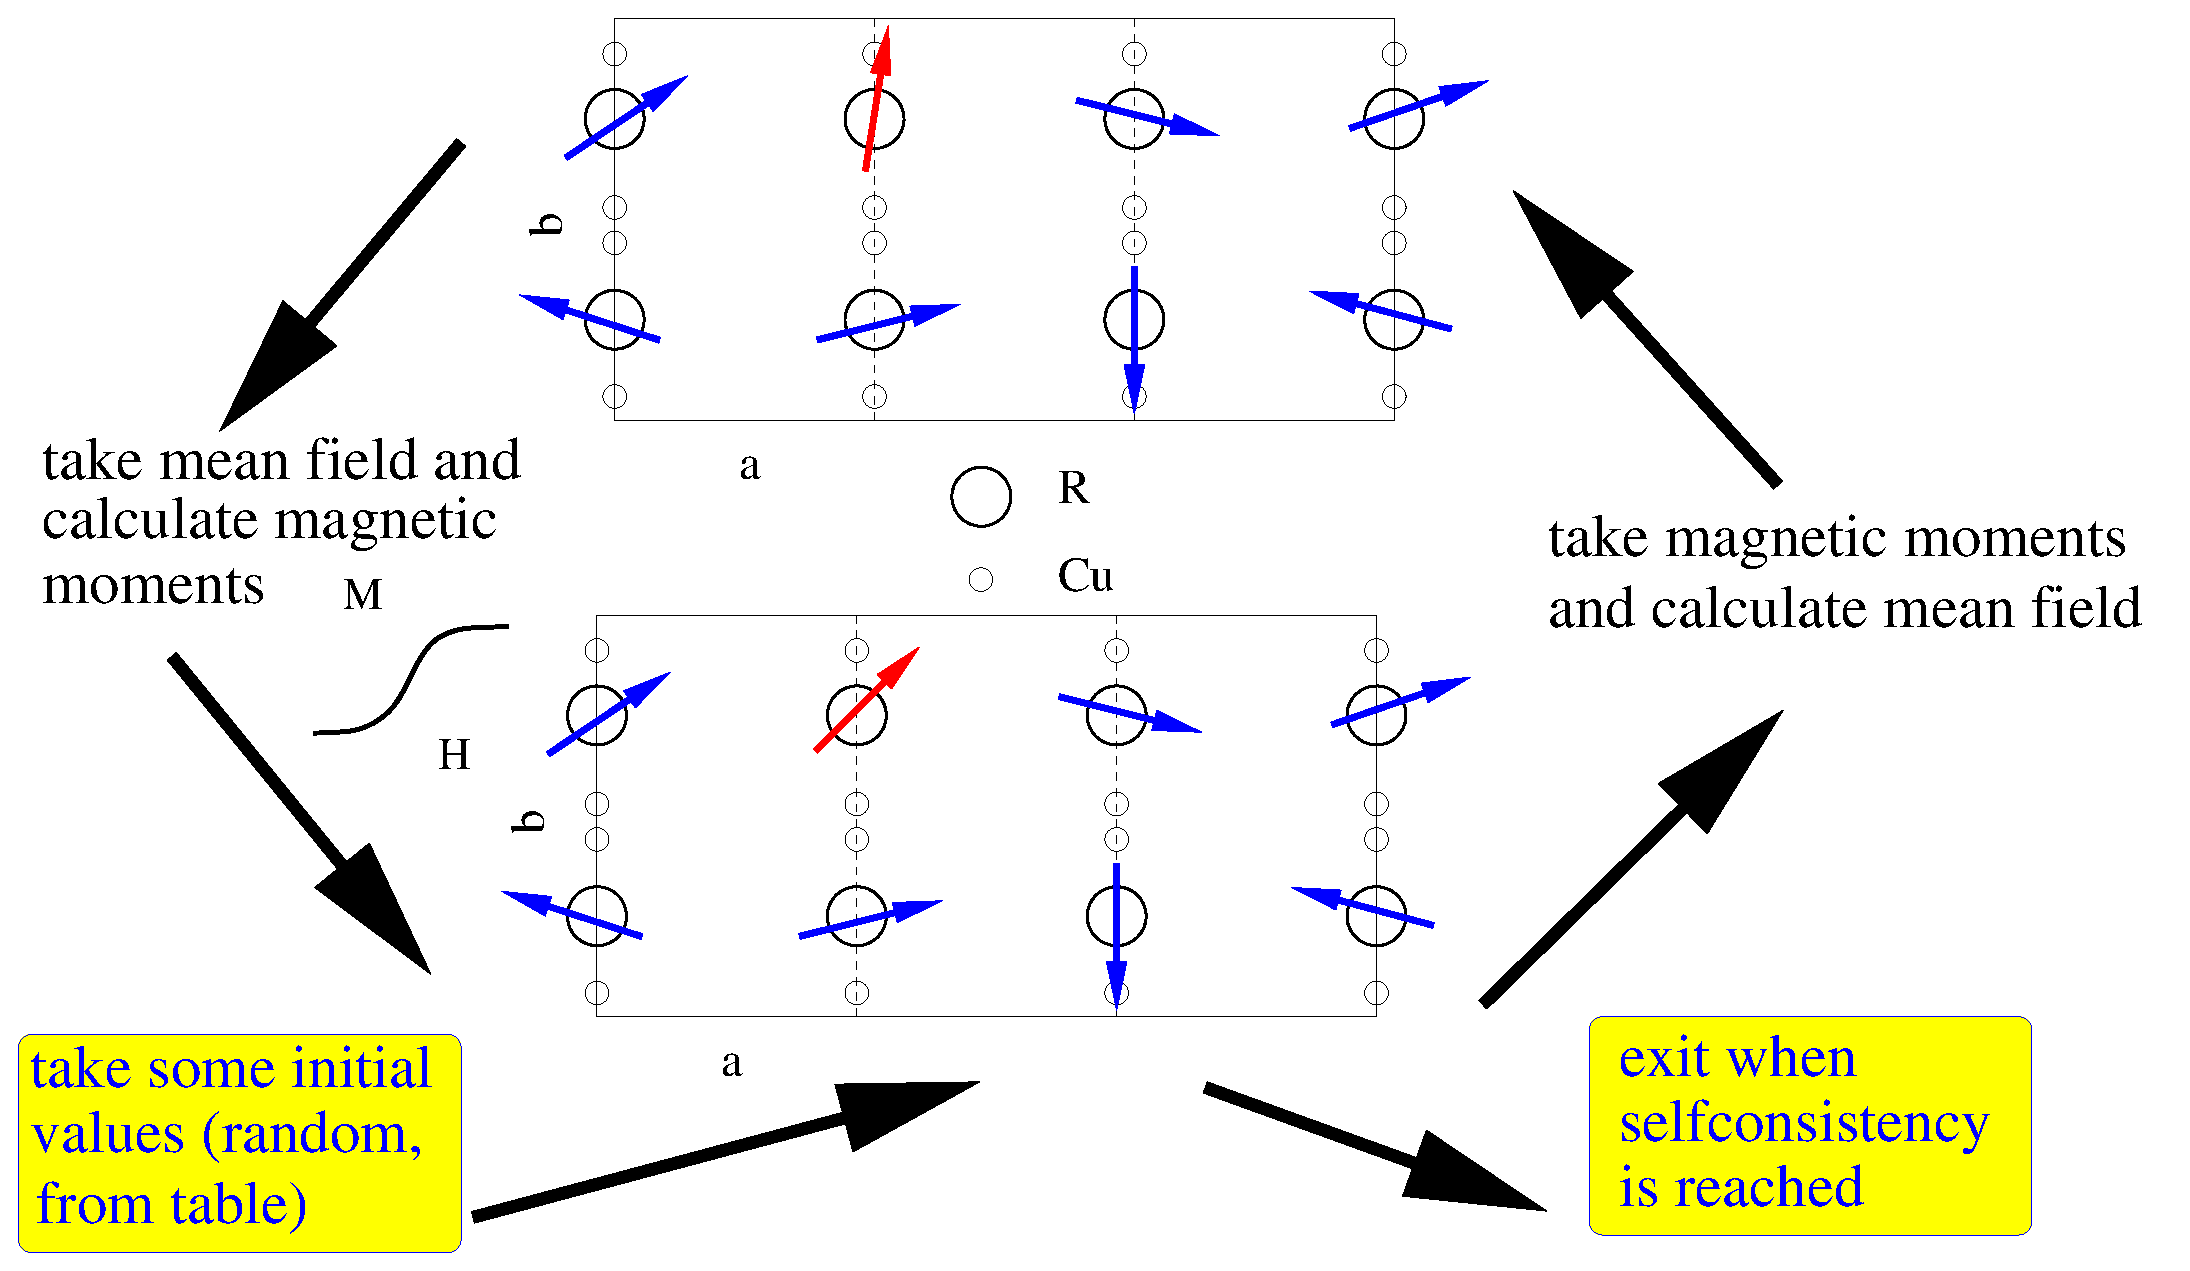
\includegraphics[angle=0,width=0.9\columnwidth]{figsrc/fecalc.eps}
\caption{\label{fecalc}Mean field process of sub {\prg fecalc}.}
\end{figure}

 
\subsubsection{Example {\prg mcphas.ini\index{mcphas.ini}} file for a simple antiferromagnet}

Here is an example of {\prg mcphas.ini\index{mcphas.ini}}, the comments describe the meaning of the different
parameters:

\section{{\prg mcphas} - calculation of thermodynamic properties (Magnetisation, Susceptibility, Specific Heat, Neutron %%@
Diffraction, etc.)}
\label{runmcphas}

In order to perform calculations beyond the capabilities of {\prg cfield\index{cfield}} it is necessary
to use the program {\prg mcphas}. 
\begin{itemize}
\item As a first step it is possible to
calculate the thermodynamic properties such as magnetisation or specific heat
considering only single ion effects. In this case all the exchange parameters
have to be set to zero in {\prg mcphas.j\index{mcphas.j}}. 
\item for more advanced calculations the two - ion interactions have to be
considered and may lead to magnetic order. {\prg mcphas} can perform 
calculations in the ordered state in the following way: for 
a given temperature $T$ and magnetic field $\mbf H$ (vector)
several possible magnetic structures are stabilised
by a mean field algorithm and the free energy is 
calculated. The initial values for this mean-field procedure are
modified by a Monte Carlo process.


The temperature and magnetic field is varied during the calculation
and thereby it is possible to map out the magnetic phase diagram.
\end{itemize}

The program produces a plot of the stabilised magnetic
structures and the magnetisation on screen, the
output files contain additional information 
such as calculated magnetoelastic and  neutron-scattering
data. Several graphic programs easy the visualisation of the
calculated data (section~\ref{graphics}).



\subsection{Input Files}
The program {\prg McPhase} needs the following input files (all in the same directory)
 in order to run:

\begin{enumerate}
\item {\prg mcphas.ini\index{mcphas.ini}}
 - controlling the algorithm
\item {\prg mcphas.j\index{mcphas.j}}
  - lattice and exchange parameters
\item {\prg mcphas.tst\index{mcphas.tst}(optional)}  - test spin configurations
\item {\prg single-ion property files}
\item {\prg directory ./results/}
 - directory where calculated data is stored
\item {\prg directory ./fit} - experimental data for fit (optional)
\end{enumerate}


 All
 of these input files have to be in one directory and the program
has to be started in this directory. The results of the simulation
are then stored in the  subdirectory ./results/, which must exist before starting
the program 
... see directory ./examples/ for some examples.
 In order to prepare these files
for a new calculation it is best to take them from an example, copy the files
to a new directory and make the
modifications  to adapt them to the new problem.

\subsubsection{Example - a simple antiferromagnet}

In the following description of the input files we will always refer
to a simple example: a simple antiferromagnet
on a primitive orthorhombic lattice. The first time user
will thus have a simple example to follow, all corresponding
files are given in the directory {\prg tutorial/03magnetic\_phases\_mcphas/simpleAF}.
 

\subsubsection{{\prg mcphas.ini\index{mcphas.ini}} - controlling the algorithm}
   Initial file containing algorithm control parameters, for instance the range and spacing of
   propagation vectors Q or the number of Monte Carlo trials for initial spin configurations
    - {\em mind}: this
   file is rewritten and reread  when running the program and may be changed by the
   user in order to manipulate the running simulation.

{\prg mcphas.ini\index{mcphas.ini}} consists of several sections:
\begin{description}
\item [MCPHASE RUNTIME CONTROL:] this section contains the parameters
controlling the status of the calculation.
\item [XY PHASEDIAGRAM PARAMETERS:] here the temperature and field range and
step widths of the calculation are specified.
The definition of the x and y
axis in terms of temperature and magnetic field is followed by the
corresponding range and step width. An offset may be given for all
field and temperature values.
Note that for most cases of interest
this offset is zero (T0=0, Ha0=0, Hb0=0, Hc0=0).
 For the simple case of calculating a Temperature-Field phase diagram
 It is just necessary to set xT=1 and give the temperature range by
xmin/xmax/xstep. For field in b direction then just set yHb=1 and 
define the range in ymin/ymax/ystep.
In case of non-orthogonal axes the applied magnetic field
components $Ha, Hb, Hc$ refer to the orthogonal coordinate system
defined with respect to the nonorthogonal lattice $\mbf a,\mbf b,\mbf c$ as
$Hb||\mbf b$, $Hc||(\mbf a \times \mbf b)$ and $Ha$ perpendicular to $Hb$ and $Hc$.

\item [GENERATION OF SPINCONFIGURATIONS:] at the beginning of the program
some initial values of spin configurations are generated from a set of 
propagation vectors. This section defines the range of propagation vectors
and the step width.
Depending on the value of the propagation Q with respect to the primitive reciprocal lattice
1-, 2- or 3-dimensional simulations of magnetic lattices
are possible. It is advisable to 
think carefully about the chosen range and spacing of Q vectors in order
to limit calculation time.
 
For example a good starting point is to begin with a calculation with large
step widths (e.g. 0.1)  covering the Brillouin zone. This should give an idea
of the propagation vectors which are stabilised. An advanced calculation
could then fine tune the propagation and determine its accurate value (using
small step widths in a limited area of the zone).
The verbose option of {\prg mcphas} allows to inspect the propagation vectors
which are actually used in the calculation.
Trick: in order to get a quick overview of the
q-vector range covered by the mcphas\index{mcphas} simulation start mcphas, exit and 
just type {\prg felog ./results/mcphas.qvc} (need {\prg perl,perldl,pdl,pgplot} packages).

In order to limit calculation time, the maximum periodicity
of the magnetic unit cell with respect to the crystallographic unit cell 
(maxqperiod) and the maximum number of spins in the magnetic unit cell 
(maxnofspins) can be limited. Also the maximum number of test spin configurations
in the internal table can be limited (maxnoftestspincf).
A critical feature with respect to calculation time is also the number of
spin configurations which are generated by a random process from a tabulated
SPINCONFIGURATIONS during the calculation. 

In summary the variables in this section are mainly important to adapt the
program to a given computer system with finite speed. They have to be set
to optimise between speed and accuracy of the calculation. In order to
find appropriate values it is best to perform some calculations 
and restrict the parameters step by step if insufficient speed is obtained.
Also the examples included in the program package may serve as starting
points.

\item [PARAMETERS FOR SUB FECALC SELFCONSISTENCY PROCESS:] the most important
procedure in the module {\prg mcphas} is the sub fecalc. In this part of the 
program the self consistent calculation of the magnetic moment configuration
is performed as shown schematically in fig.~\ref{fecalc}. 
In the mean field approximation the Hamiltonian~(\ref{hamilton}) is approximated
by

\begin{equation}
 {\mathcal H}=\sum_n H_{SI}^n + E_{corr}
\end{equation}

with the single ion Hamiltonian (in case of module {\prg so1ion\index{so1ion}})

\begin{equation}
H_{SI}^n=  B_l^m O_{lm}({\mbf J}^n) 
	     - g_{Jn} \mu_B {\mbf J}^n {\mbf H^n_{eff}} 
\end{equation}

and the correction term

\begin{equation}
E_{corr}=\frac{1}{2}\sum_{n} g_{Jn} \mu_B \langle {\mbf J}^n
 \rangle (\mbf H^n_{eff}-\mbf H) 
\end{equation}

and with the mean fields $ \mbf H^n_{eff}$ given by

\begin{equation}\label{meanfield}
\mbf H^n_{eff}=\mbf H + \mbf H^n_{xc}=\mbf H+\sum_{{\mbf G'}n'} \frac{{\mathcal J}
(\mbf r_n-(\mbf G'+\mbf r_{n'}))}{g_{Jn}\mu_B } \langle{\mbf
J}^{n'}\rangle
\end{equation}

These mean fields and the moments $\langle \mbf J^n \rangle$ 
are determined in a self consistent
way. For a given magnetic unit cell and initial configuration 
of magnetic moments
the mean fields are calculated according to equation~(\ref{meanfield}). 
Then, for each
magnetic ion the single ion property module is taken 
and the magnetic moment $\langle \mbf J^n \rangle$ is 
calculated from it's mean field. The mean fields are used again in equation~(\ref{meanfield})
and so on .... until convergence is reached. 
Then, the free energy ($f=-kT\sum_n \ln(z_n) + E_{corr}$ ) 
of the stabilised
configuration is calculated (this is why this sub is called {\prg fecalc}). 
The free energies of a lot of different stabilised configurations have to
be compared in order to find out which configuration has lowest free energy, i.e.
is stable in thermal  equilibrium.

It may happen that this process does
not converge due to bad choice of the initial configuration, therefore a maximum number
of mean field loops has to be given by the user.
The results of a calculation may be significantly influenced by
changing parameters such as the maximum number of iteration loops 
in this section. 
In fact the simulation is always a compromise of calculation time and accuracy: if only
a few initial spin configurations are tried at each (H-T) point, the calculation speed is
fast, however it is possible that the program misses the magnetic structure with the
lowest free energy. The same holds if other critical parameters of the simulation are
restricted too much.
 

\item [OUTPUT OF PHYSICAL PROPERTIES:]
Some options for the output of the calculation can be changed in this section.
\end{description}

\begin{figure}[hb]
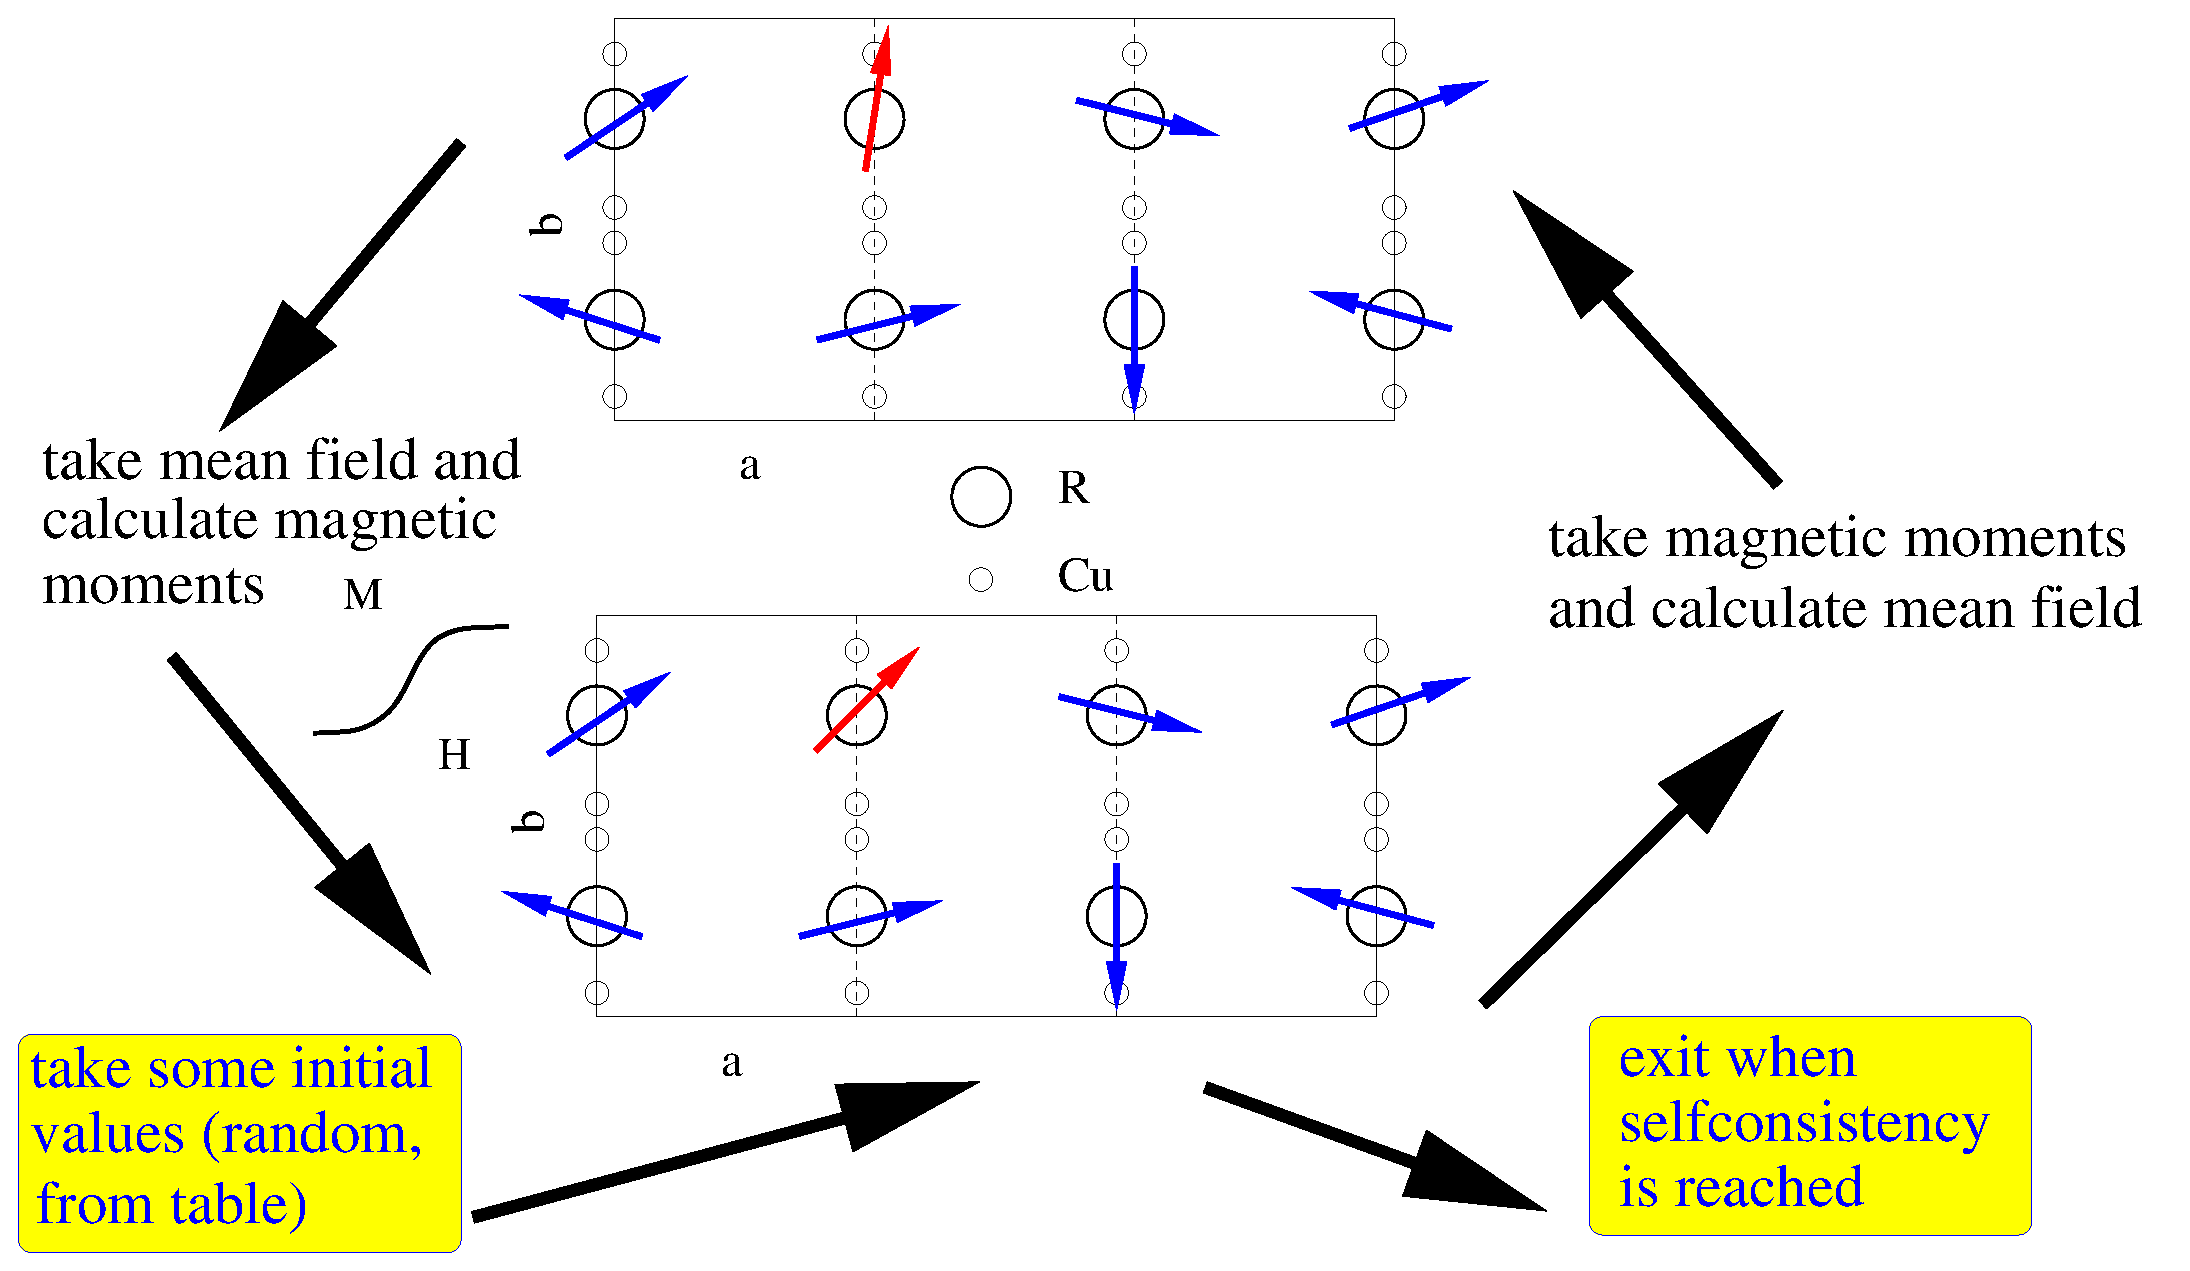
\includegraphics[angle=0,width=0.9\columnwidth]{figsrc/fecalc.eps}
\caption{\label{fecalc}Mean field process of sub {\prg fecalc}.}
\end{figure}

 
\subsubsection{Example {\prg mcphas.ini\index{mcphas.ini}} file for a simple antiferromagnet}

Here is an example of {\prg mcphas.ini\index{mcphas.ini}}, the comments describe the meaning of the different
parameters:

\section{{\prg mcphas} - calculation of thermodynamic properties (Magnetisation, Susceptibility, Specific Heat, Neutron %%@
Diffraction, etc.)}
\label{runmcphas}

In order to perform calculations beyond the capabilities of {\prg cfield\index{cfield}} it is necessary
to use the program {\prg mcphas}. 
\begin{itemize}
\item As a first step it is possible to
calculate the thermodynamic properties such as magnetisation or specific heat
considering only single ion effects. In this case all the exchange parameters
have to be set to zero in {\prg mcphas.j\index{mcphas.j}}. 
\item for more advanced calculations the two - ion interactions have to be
considered and may lead to magnetic order. {\prg mcphas} can perform 
calculations in the ordered state in the following way: for 
a given temperature $T$ and magnetic field $\mbf H$ (vector)
several possible magnetic structures are stabilised
by a mean field algorithm and the free energy is 
calculated. The initial values for this mean-field procedure are
modified by a Monte Carlo process.


The temperature and magnetic field is varied during the calculation
and thereby it is possible to map out the magnetic phase diagram.
\end{itemize}

The program produces a plot of the stabilised magnetic
structures and the magnetisation on screen, the
output files contain additional information 
such as calculated magnetoelastic and  neutron-scattering
data. Several graphic programs easy the visualisation of the
calculated data (section~\ref{graphics}).



\subsection{Input Files}
The program {\prg McPhase} needs the following input files (all in the same directory)
 in order to run:

\begin{enumerate}
\item {\prg mcphas.ini\index{mcphas.ini}}
 - controlling the algorithm
\item {\prg mcphas.j\index{mcphas.j}}
  - lattice and exchange parameters
\item {\prg mcphas.tst\index{mcphas.tst}(optional)}  - test spin configurations
\item {\prg single-ion property files}
\item {\prg directory ./results/}
 - directory where calculated data is stored
\item {\prg directory ./fit} - experimental data for fit (optional)
\end{enumerate}


 All
 of these input files have to be in one directory and the program
has to be started in this directory. The results of the simulation
are then stored in the  subdirectory ./results/, which must exist before starting
the program 
... see directory ./examples/ for some examples.
 In order to prepare these files
for a new calculation it is best to take them from an example, copy the files
to a new directory and make the
modifications  to adapt them to the new problem.

\subsubsection{Example - a simple antiferromagnet}

In the following description of the input files we will always refer
to a simple example: a simple antiferromagnet
on a primitive orthorhombic lattice. The first time user
will thus have a simple example to follow, all corresponding
files are given in the directory {\prg tutorial/03magnetic\_phases\_mcphas/simpleAF}.
 

\subsubsection{{\prg mcphas.ini\index{mcphas.ini}} - controlling the algorithm}
   Initial file containing algorithm control parameters, for instance the range and spacing of
   propagation vectors Q or the number of Monte Carlo trials for initial spin configurations
    - {\em mind}: this
   file is rewritten and reread  when running the program and may be changed by the
   user in order to manipulate the running simulation.

{\prg mcphas.ini\index{mcphas.ini}} consists of several sections:
\begin{description}
\item [MCPHASE RUNTIME CONTROL:] this section contains the parameters
controlling the status of the calculation.
\item [XY PHASEDIAGRAM PARAMETERS:] here the temperature and field range and
step widths of the calculation are specified.
The definition of the x and y
axis in terms of temperature and magnetic field is followed by the
corresponding range and step width. An offset may be given for all
field and temperature values.
Note that for most cases of interest
this offset is zero (T0=0, Ha0=0, Hb0=0, Hc0=0).
 For the simple case of calculating a Temperature-Field phase diagram
 It is just necessary to set xT=1 and give the temperature range by
xmin/xmax/xstep. For field in b direction then just set yHb=1 and 
define the range in ymin/ymax/ystep.
In case of non-orthogonal axes the applied magnetic field
components $Ha, Hb, Hc$ refer to the orthogonal coordinate system
defined with respect to the nonorthogonal lattice $\mbf a,\mbf b,\mbf c$ as
$Hb||\mbf b$, $Hc||(\mbf a \times \mbf b)$ and $Ha$ perpendicular to $Hb$ and $Hc$.

\item [GENERATION OF SPINCONFIGURATIONS:] at the beginning of the program
some initial values of spin configurations are generated from a set of 
propagation vectors. This section defines the range of propagation vectors
and the step width.
Depending on the value of the propagation Q with respect to the primitive reciprocal lattice
1-, 2- or 3-dimensional simulations of magnetic lattices
are possible. It is advisable to 
think carefully about the chosen range and spacing of Q vectors in order
to limit calculation time.
 
For example a good starting point is to begin with a calculation with large
step widths (e.g. 0.1)  covering the Brillouin zone. This should give an idea
of the propagation vectors which are stabilised. An advanced calculation
could then fine tune the propagation and determine its accurate value (using
small step widths in a limited area of the zone).
The verbose option of {\prg mcphas} allows to inspect the propagation vectors
which are actually used in the calculation.
Trick: in order to get a quick overview of the
q-vector range covered by the mcphas\index{mcphas} simulation start mcphas, exit and 
just type {\prg felog ./results/mcphas.qvc} (need {\prg perl,perldl,pdl,pgplot} packages).

In order to limit calculation time, the maximum periodicity
of the magnetic unit cell with respect to the crystallographic unit cell 
(maxqperiod) and the maximum number of spins in the magnetic unit cell 
(maxnofspins) can be limited. Also the maximum number of test spin configurations
in the internal table can be limited (maxnoftestspincf).
A critical feature with respect to calculation time is also the number of
spin configurations which are generated by a random process from a tabulated
SPINCONFIGURATIONS during the calculation. 

In summary the variables in this section are mainly important to adapt the
program to a given computer system with finite speed. They have to be set
to optimise between speed and accuracy of the calculation. In order to
find appropriate values it is best to perform some calculations 
and restrict the parameters step by step if insufficient speed is obtained.
Also the examples included in the program package may serve as starting
points.

\item [PARAMETERS FOR SUB FECALC SELFCONSISTENCY PROCESS:] the most important
procedure in the module {\prg mcphas} is the sub fecalc. In this part of the 
program the self consistent calculation of the magnetic moment configuration
is performed as shown schematically in fig.~\ref{fecalc}. 
In the mean field approximation the Hamiltonian~(\ref{hamilton}) is approximated
by

\begin{equation}
 {\mathcal H}=\sum_n H_{SI}^n + E_{corr}
\end{equation}

with the single ion Hamiltonian (in case of module {\prg so1ion\index{so1ion}})

\begin{equation}
H_{SI}^n=  B_l^m O_{lm}({\mbf J}^n) 
	     - g_{Jn} \mu_B {\mbf J}^n {\mbf H^n_{eff}} 
\end{equation}

and the correction term

\begin{equation}
E_{corr}=\frac{1}{2}\sum_{n} g_{Jn} \mu_B \langle {\mbf J}^n
 \rangle (\mbf H^n_{eff}-\mbf H) 
\end{equation}

and with the mean fields $ \mbf H^n_{eff}$ given by

\begin{equation}\label{meanfield}
\mbf H^n_{eff}=\mbf H + \mbf H^n_{xc}=\mbf H+\sum_{{\mbf G'}n'} \frac{{\mathcal J}
(\mbf r_n-(\mbf G'+\mbf r_{n'}))}{g_{Jn}\mu_B } \langle{\mbf
J}^{n'}\rangle
\end{equation}

These mean fields and the moments $\langle \mbf J^n \rangle$ 
are determined in a self consistent
way. For a given magnetic unit cell and initial configuration 
of magnetic moments
the mean fields are calculated according to equation~(\ref{meanfield}). 
Then, for each
magnetic ion the single ion property module is taken 
and the magnetic moment $\langle \mbf J^n \rangle$ is 
calculated from it's mean field. The mean fields are used again in equation~(\ref{meanfield})
and so on .... until convergence is reached. 
Then, the free energy ($f=-kT\sum_n \ln(z_n) + E_{corr}$ ) 
of the stabilised
configuration is calculated (this is why this sub is called {\prg fecalc}). 
The free energies of a lot of different stabilised configurations have to
be compared in order to find out which configuration has lowest free energy, i.e.
is stable in thermal  equilibrium.

It may happen that this process does
not converge due to bad choice of the initial configuration, therefore a maximum number
of mean field loops has to be given by the user.
The results of a calculation may be significantly influenced by
changing parameters such as the maximum number of iteration loops 
in this section. 
In fact the simulation is always a compromise of calculation time and accuracy: if only
a few initial spin configurations are tried at each (H-T) point, the calculation speed is
fast, however it is possible that the program misses the magnetic structure with the
lowest free energy. The same holds if other critical parameters of the simulation are
restricted too much.
 

\item [OUTPUT OF PHYSICAL PROPERTIES:]
Some options for the output of the calculation can be changed in this section.
\end{description}

\begin{figure}[hb]
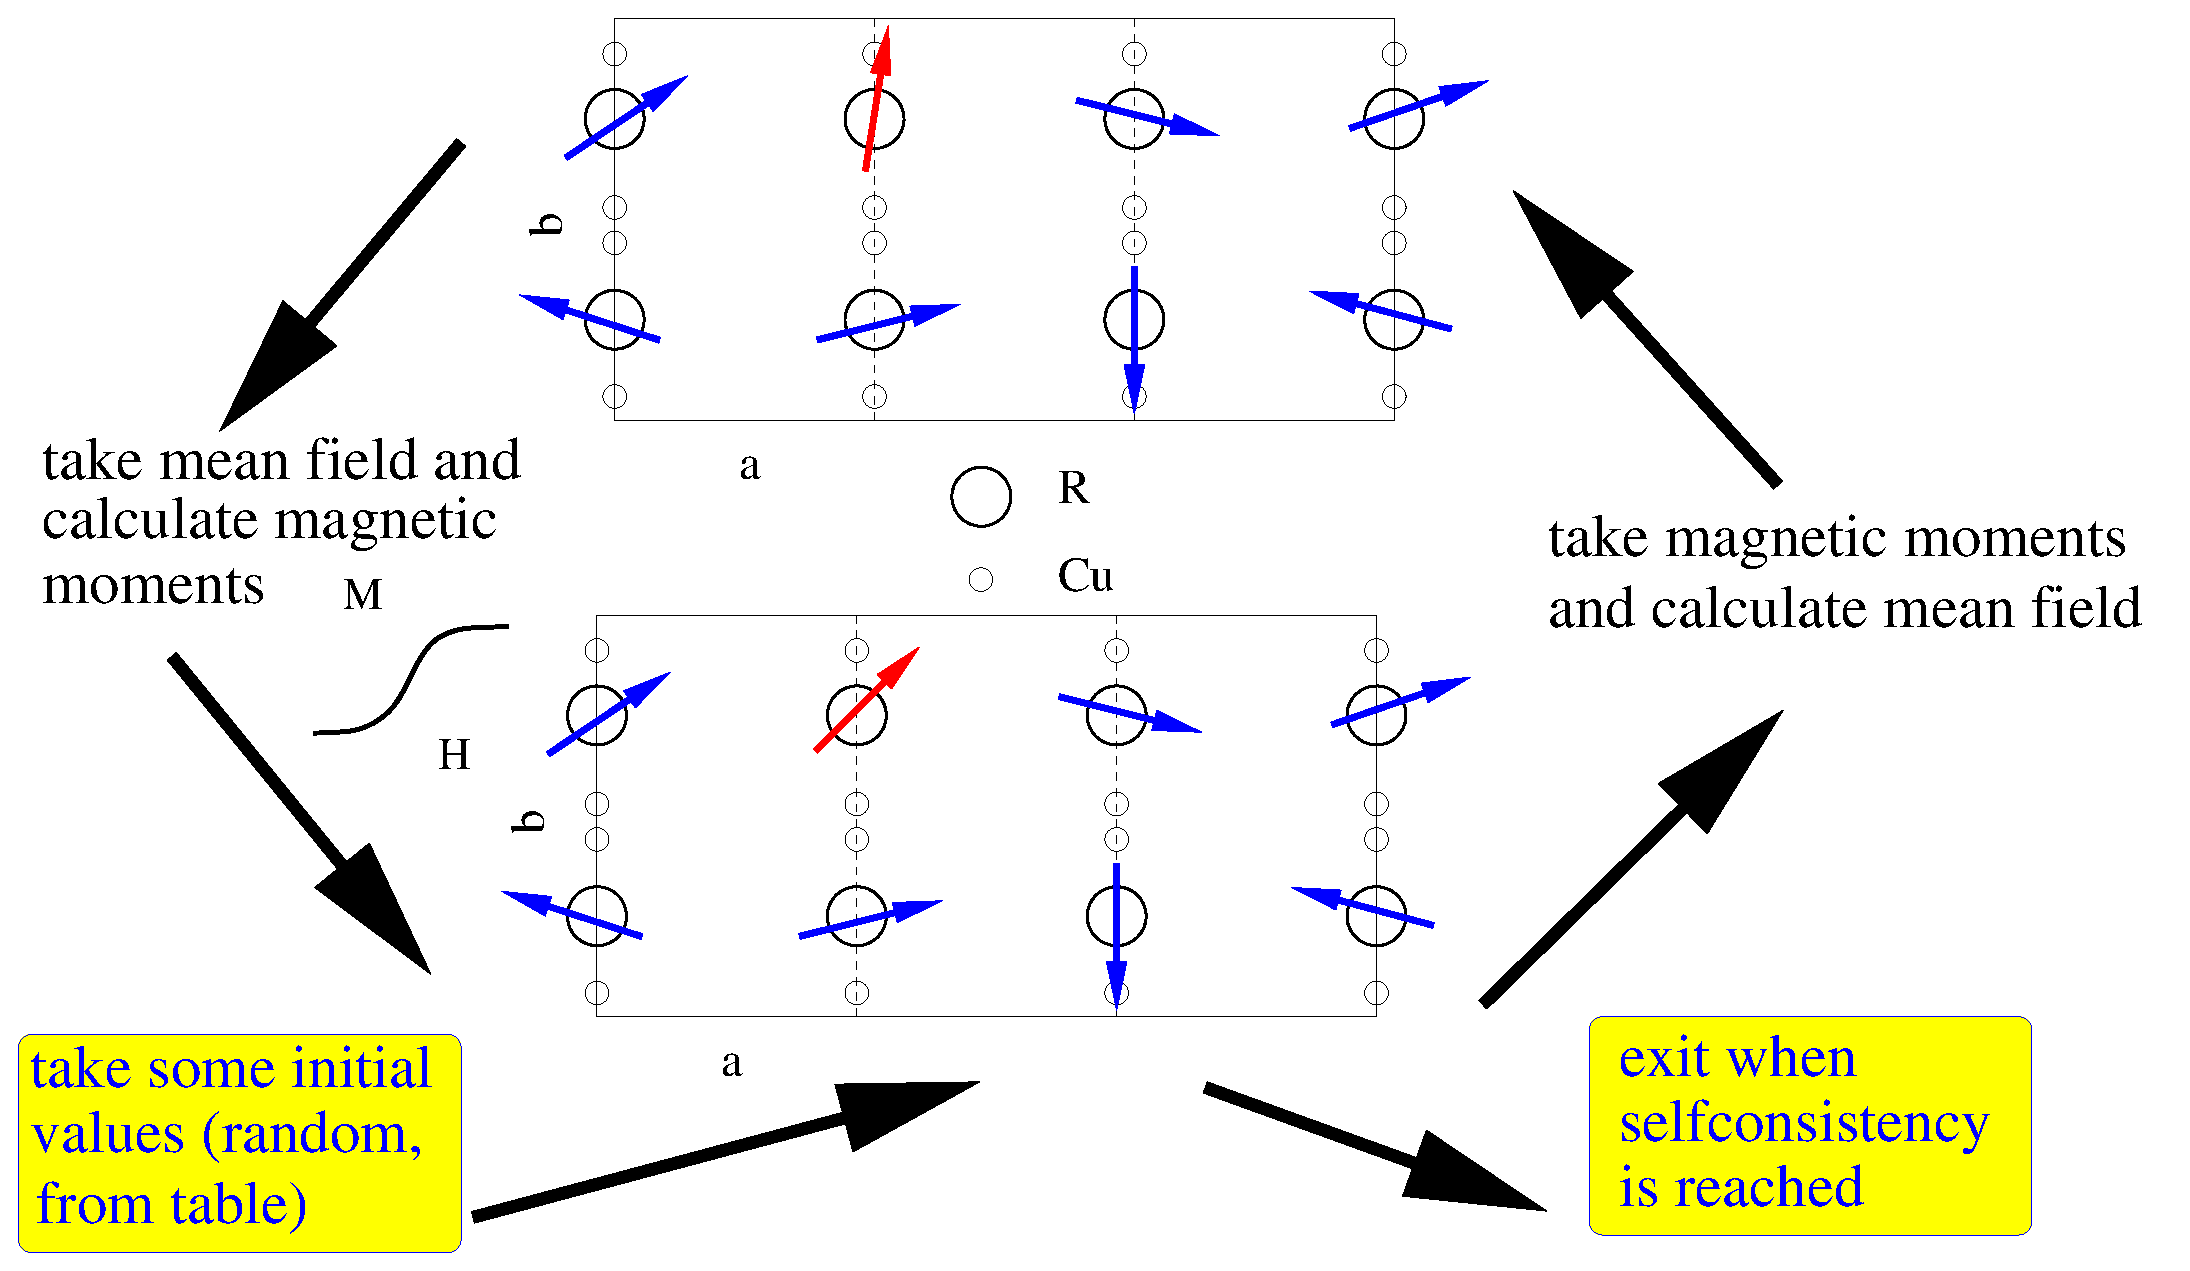
\includegraphics[angle=0,width=0.9\columnwidth]{figsrc/fecalc.eps}
\caption{\label{fecalc}Mean field process of sub {\prg fecalc}.}
\end{figure}

 
\subsubsection{Example {\prg mcphas.ini\index{mcphas.ini}} file for a simple antiferromagnet}

Here is an example of {\prg mcphas.ini\index{mcphas.ini}}, the comments describe the meaning of the different
parameters:

\section{{\prg mcphas} - calculation of thermodynamic properties (Magnetisation, Susceptibility, Specific Heat, Neutron %%@
Diffraction, etc.)}
\label{runmcphas}

In order to perform calculations beyond the capabilities of {\prg cfield\index{cfield}} it is necessary
to use the program {\prg mcphas}. 
\begin{itemize}
\item As a first step it is possible to
calculate the thermodynamic properties such as magnetisation or specific heat
considering only single ion effects. In this case all the exchange parameters
have to be set to zero in {\prg mcphas.j\index{mcphas.j}}. 
\item for more advanced calculations the two - ion interactions have to be
considered and may lead to magnetic order. {\prg mcphas} can perform 
calculations in the ordered state in the following way: for 
a given temperature $T$ and magnetic field $\mbf H$ (vector)
several possible magnetic structures are stabilised
by a mean field algorithm and the free energy is 
calculated. The initial values for this mean-field procedure are
modified by a Monte Carlo process.


The temperature and magnetic field is varied during the calculation
and thereby it is possible to map out the magnetic phase diagram.
\end{itemize}

The program produces a plot of the stabilised magnetic
structures and the magnetisation on screen, the
output files contain additional information 
such as calculated magnetoelastic and  neutron-scattering
data. Several graphic programs easy the visualisation of the
calculated data (section~\ref{graphics}).



\subsection{Input Files}
The program {\prg McPhase} needs the following input files (all in the same directory)
 in order to run:

\begin{enumerate}
\item {\prg mcphas.ini\index{mcphas.ini}}
 - controlling the algorithm
\item {\prg mcphas.j\index{mcphas.j}}
  - lattice and exchange parameters
\item {\prg mcphas.tst\index{mcphas.tst}(optional)}  - test spin configurations
\item {\prg single-ion property files}
\item {\prg directory ./results/}
 - directory where calculated data is stored
\item {\prg directory ./fit} - experimental data for fit (optional)
\end{enumerate}


 All
 of these input files have to be in one directory and the program
has to be started in this directory. The results of the simulation
are then stored in the  subdirectory ./results/, which must exist before starting
the program 
... see directory ./examples/ for some examples.
 In order to prepare these files
for a new calculation it is best to take them from an example, copy the files
to a new directory and make the
modifications  to adapt them to the new problem.

\subsubsection{Example - a simple antiferromagnet}

In the following description of the input files we will always refer
to a simple example: a simple antiferromagnet
on a primitive orthorhombic lattice. The first time user
will thus have a simple example to follow, all corresponding
files are given in the directory {\prg tutorial/03magnetic\_phases\_mcphas/simpleAF}.
 

\subsubsection{{\prg mcphas.ini\index{mcphas.ini}} - controlling the algorithm}
   Initial file containing algorithm control parameters, for instance the range and spacing of
   propagation vectors Q or the number of Monte Carlo trials for initial spin configurations
    - {\em mind}: this
   file is rewritten and reread  when running the program and may be changed by the
   user in order to manipulate the running simulation.

{\prg mcphas.ini\index{mcphas.ini}} consists of several sections:
\begin{description}
\item [MCPHASE RUNTIME CONTROL:] this section contains the parameters
controlling the status of the calculation.
\item [XY PHASEDIAGRAM PARAMETERS:] here the temperature and field range and
step widths of the calculation are specified.
The definition of the x and y
axis in terms of temperature and magnetic field is followed by the
corresponding range and step width. An offset may be given for all
field and temperature values.
Note that for most cases of interest
this offset is zero (T0=0, Ha0=0, Hb0=0, Hc0=0).
 For the simple case of calculating a Temperature-Field phase diagram
 It is just necessary to set xT=1 and give the temperature range by
xmin/xmax/xstep. For field in b direction then just set yHb=1 and 
define the range in ymin/ymax/ystep.
In case of non-orthogonal axes the applied magnetic field
components $Ha, Hb, Hc$ refer to the orthogonal coordinate system
defined with respect to the nonorthogonal lattice $\mbf a,\mbf b,\mbf c$ as
$Hb||\mbf b$, $Hc||(\mbf a \times \mbf b)$ and $Ha$ perpendicular to $Hb$ and $Hc$.

\item [GENERATION OF SPINCONFIGURATIONS:] at the beginning of the program
some initial values of spin configurations are generated from a set of 
propagation vectors. This section defines the range of propagation vectors
and the step width.
Depending on the value of the propagation Q with respect to the primitive reciprocal lattice
1-, 2- or 3-dimensional simulations of magnetic lattices
are possible. It is advisable to 
think carefully about the chosen range and spacing of Q vectors in order
to limit calculation time.
 
For example a good starting point is to begin with a calculation with large
step widths (e.g. 0.1)  covering the Brillouin zone. This should give an idea
of the propagation vectors which are stabilised. An advanced calculation
could then fine tune the propagation and determine its accurate value (using
small step widths in a limited area of the zone).
The verbose option of {\prg mcphas} allows to inspect the propagation vectors
which are actually used in the calculation.
Trick: in order to get a quick overview of the
q-vector range covered by the mcphas\index{mcphas} simulation start mcphas, exit and 
just type {\prg felog ./results/mcphas.qvc} (need {\prg perl,perldl,pdl,pgplot} packages).

In order to limit calculation time, the maximum periodicity
of the magnetic unit cell with respect to the crystallographic unit cell 
(maxqperiod) and the maximum number of spins in the magnetic unit cell 
(maxnofspins) can be limited. Also the maximum number of test spin configurations
in the internal table can be limited (maxnoftestspincf).
A critical feature with respect to calculation time is also the number of
spin configurations which are generated by a random process from a tabulated
SPINCONFIGURATIONS during the calculation. 

In summary the variables in this section are mainly important to adapt the
program to a given computer system with finite speed. They have to be set
to optimise between speed and accuracy of the calculation. In order to
find appropriate values it is best to perform some calculations 
and restrict the parameters step by step if insufficient speed is obtained.
Also the examples included in the program package may serve as starting
points.

\item [PARAMETERS FOR SUB FECALC SELFCONSISTENCY PROCESS:] the most important
procedure in the module {\prg mcphas} is the sub fecalc. In this part of the 
program the self consistent calculation of the magnetic moment configuration
is performed as shown schematically in fig.~\ref{fecalc}. 
In the mean field approximation the Hamiltonian~(\ref{hamilton}) is approximated
by

\begin{equation}
 {\mathcal H}=\sum_n H_{SI}^n + E_{corr}
\end{equation}

with the single ion Hamiltonian (in case of module {\prg so1ion\index{so1ion}})

\begin{equation}
H_{SI}^n=  B_l^m O_{lm}({\mbf J}^n) 
	     - g_{Jn} \mu_B {\mbf J}^n {\mbf H^n_{eff}} 
\end{equation}

and the correction term

\begin{equation}
E_{corr}=\frac{1}{2}\sum_{n} g_{Jn} \mu_B \langle {\mbf J}^n
 \rangle (\mbf H^n_{eff}-\mbf H) 
\end{equation}

and with the mean fields $ \mbf H^n_{eff}$ given by

\begin{equation}\label{meanfield}
\mbf H^n_{eff}=\mbf H + \mbf H^n_{xc}=\mbf H+\sum_{{\mbf G'}n'} \frac{{\mathcal J}
(\mbf r_n-(\mbf G'+\mbf r_{n'}))}{g_{Jn}\mu_B } \langle{\mbf
J}^{n'}\rangle
\end{equation}

These mean fields and the moments $\langle \mbf J^n \rangle$ 
are determined in a self consistent
way. For a given magnetic unit cell and initial configuration 
of magnetic moments
the mean fields are calculated according to equation~(\ref{meanfield}). 
Then, for each
magnetic ion the single ion property module is taken 
and the magnetic moment $\langle \mbf J^n \rangle$ is 
calculated from it's mean field. The mean fields are used again in equation~(\ref{meanfield})
and so on .... until convergence is reached. 
Then, the free energy ($f=-kT\sum_n \ln(z_n) + E_{corr}$ ) 
of the stabilised
configuration is calculated (this is why this sub is called {\prg fecalc}). 
The free energies of a lot of different stabilised configurations have to
be compared in order to find out which configuration has lowest free energy, i.e.
is stable in thermal  equilibrium.

It may happen that this process does
not converge due to bad choice of the initial configuration, therefore a maximum number
of mean field loops has to be given by the user.
The results of a calculation may be significantly influenced by
changing parameters such as the maximum number of iteration loops 
in this section. 
In fact the simulation is always a compromise of calculation time and accuracy: if only
a few initial spin configurations are tried at each (H-T) point, the calculation speed is
fast, however it is possible that the program misses the magnetic structure with the
lowest free energy. The same holds if other critical parameters of the simulation are
restricted too much.
 

\item [OUTPUT OF PHYSICAL PROPERTIES:]
Some options for the output of the calculation can be changed in this section.
\end{description}

\begin{figure}[hb]
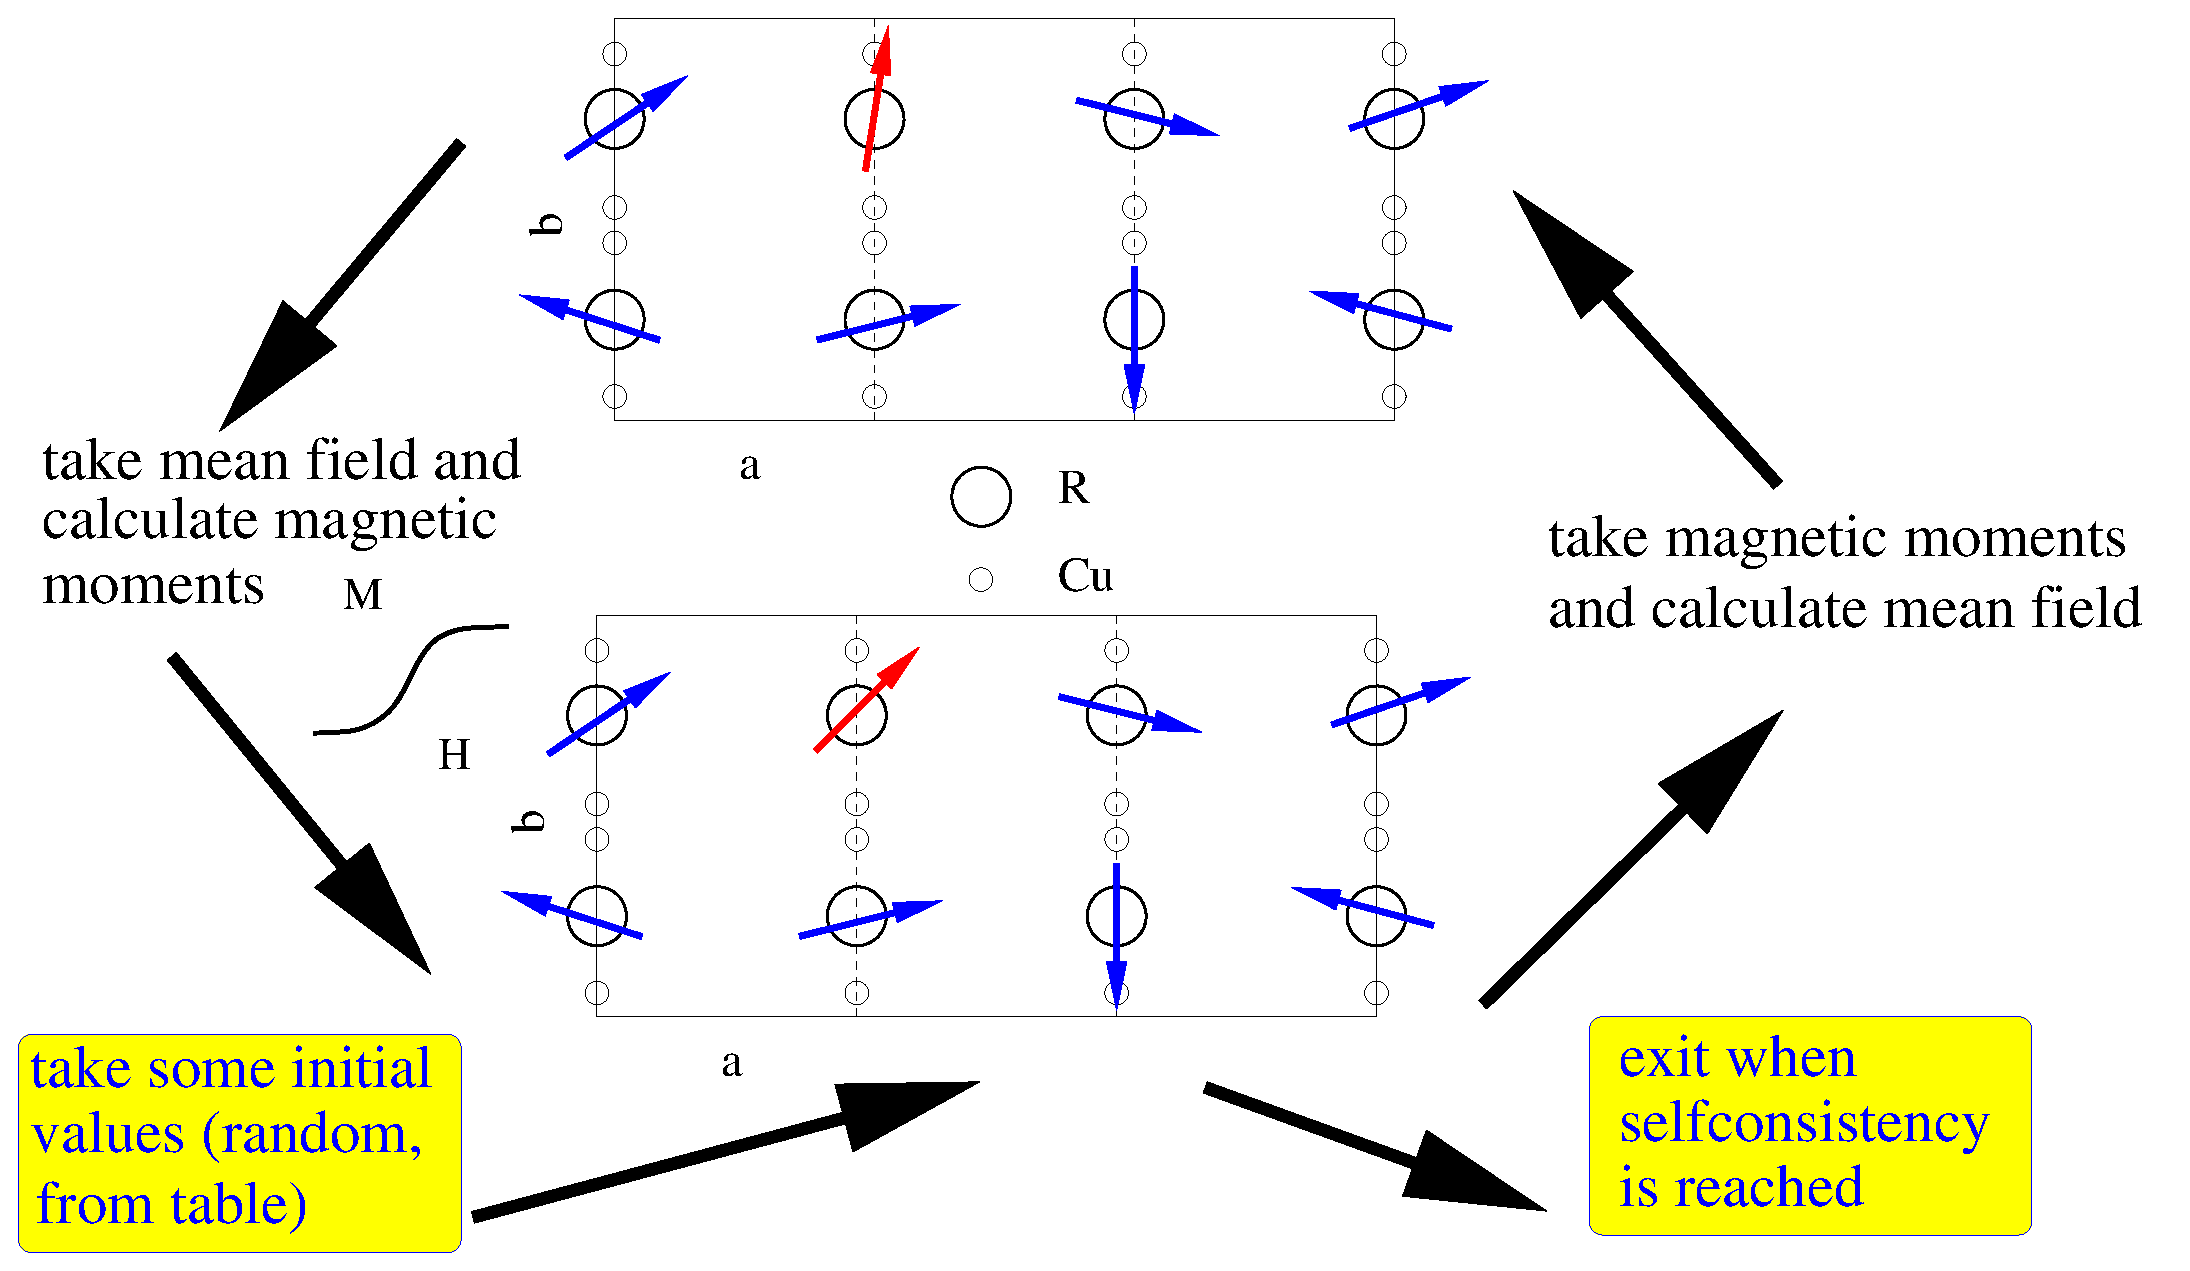
\includegraphics[angle=0,width=0.9\columnwidth]{figsrc/fecalc.eps}
\caption{\label{fecalc}Mean field process of sub {\prg fecalc}.}
\end{figure}

 
\subsubsection{Example {\prg mcphas.ini\index{mcphas.ini}} file for a simple antiferromagnet}

Here is an example of {\prg mcphas.ini\index{mcphas.ini}}, the comments describe the meaning of the different
parameters:

\input{mcphas.ini}



\subsubsection{{\prg mcphas.j\index{mcphas.j}} - lattice and exchange parameters}\label{mcphasj}
This file provides the information about 
the crystallographic
 structure and the magnetic exchange interactions.
For every atom in the crystallographic basis there
has to be given the coordinates, the number of neighbours to be considered, the 
Land\'e factor $g_J$, the single ion property filename and  a set of exchange parameters.
If the exchange parameters (and neighbour positions) are not known for your system, you 
can use the program module {\prg makenn\index{makenn}} (see section \ref{addprog}) to generate 
a list of nearest neighbours and
exchange parameters, currently implemented in {\prg makenn\index{makenn}} are dipolar interactions,
exchange interactions via the Bethe-Slater curve or the RKKY model. Note that in order
to use {\prg makenn\index{makenn}} you have to set up a working {\prg mcphas.j\index{mcphas.j}} file, which may or
may not contain neighbours and interactions.

Use program {\prg addj\index{addj}} to add exchange parameter set stored in different 
such {\prg .j} files (see section~\ref{addprog}).



\begin{description}
\item [Line 1,2:] Comment Lines
\item [Line 3:] lattice constants a,b,c and crystal angles alpha, beta, gamma 
\item [Line 4-6:] primitive lattice vectors
\item [Line 7:] Number of atoms in the primitive crystallographic unit cell ({\prg nofatoms})
\item [Line 8:] a comment line with stars
\item [Line 9:] coordinates  ($d_a$,$d_b$,$d_c$) of 1$^{st}$ magnetic ion in the crystallographic unit cell  with
respect to the lattice vectors $\vec a$,$\vec b$,$\vec c$. The number of neighbours of this 
ion, for which interaction constants are given in the interaction table (nofneighbours). 
If {\prg diagonalexchange}
is set to 0 the 9 components of the exchange tensor are given in column 4-12. 
If {\prg diagonalexchange}
 is 1, only 3 components are given (column 4-6).
If {\prg diagonalexchange}
 is 2, specific components of the exchange tensor can be given in columns 4 onwards. The indices of these components
 must be given in the following line (Line 9a below).
The Land\'e factor of the ion (gJ) and the file name of the corresponding single ion
parameter file (cffilename).
\item [Line 9a:]  If {\prg diagonalexchange=2}, then this line gives the indices of the exchange tensor corresponding to 
 the columns 4 onwards. It must have a variable called {\prg indexexchange} followed by a list of names of components of the interaction
 tensor separated by space. E.g.
 \verb|  #! indexexchange= JaJb JbJc  | 
means column 4 gives the the interaction constant between the
 first angular momentum component of the current ion with the second angular momentum component of its neighbour, whilst 
 column 5 has the interaction constant between the second angular momentum component of this ion with the third component of its
 neighbour. Alternatively, pairs of numbers may be given, as in \verb|  #! indexexchange= 1,2 2,3  |
 Additionally another parameter {\prg symmetricexchange} can be set to 1, where the value in each column is also used 
 for the transposed tensor component. Thus \verb|  #! symmetricexchange=1 indexexchange= JaJb  | is the same as \\
 \verb|  #! indexexchange= JaJb JbJa  | where the 4th and 5th column are the same.
\item [Line 10:]  Comment line
\item [Line 11-(10+nofneighbours):] Interaction table for ion number 1.   
Note: the neighbour coordinates (column 1-3) are given with respect to the lattice vectors
$\vec a$,$\vec b$,$\vec c$. The program then calculates from these values the coordinates
with respect to the primitive lattice $\vec r_1$,~$\vec r_2$,~$\vec r_3$.
($ d_a \vec a + d_b \vec b + d_c \vec c = d_1 \vec r_1 + d_2 \vec r_2 + d_3 \vec r_3$).
Column 4,5,6 \dots contain the components of the interaction tensor $\stackrel{=}{\mathcal J}$. 
Note that in case of non-orthogonal axes the 
components of the moments and the interaction tensor $Ja, Jb, Jc, Jaa, Jbb, Jcc, Jab ...$ 
refer to the orthogonal coordinate system
defined with respect to the nonorthogonal lattice $\vec a,\vec b,\vec c$ as
$Jb||\vec b$, $Jc||(\vec a \times \vec b)$ and $Ja$ perpendicular to $Jb$ and $Jc$.
\item [Line (11+nofneighbours) - end:] for each ion in the unit cell line 8 - (10+nofneighbours)
are repeated.
\end{description}


\vspace{0.5cm}

{\small {\bf Information for experienced users:}
\begin{description}
\item[\prg mcphas.jjj:]
format of exchange parameter file, which only needs a reduced set of exchange
parameters in the input file. Using the program {\prg jjj2j} the file can be transformed
to {\prg mcphas.j\index{mcphas.j}} by adding lines for all the equivalent neighbours. The format definition
of {\prg mcphas.jjj} is the same as {\prg mcphas.j\index{mcphas.j}}, however each line denotes several
equivalent neighbour atoms (instead of only one in {\prg mcphas.j\index{mcphas.j}}) according to the
 following rules:
\begin{itemize}
\item If a nonzero coordinate $d_a$ (or $d_b$,$d_c$) in the interaction table
 corresponds to it's value at the nearest
 lattice point of the primitive lattice,
  additional interactions of the same size
with  neighbours with coordinate $-d_a$ (or $-d_b$,$-d_c$, respectively)
are taken into account. This
holds for each of the three coordinates $d_a$,$d_b$ and $d_c$
 resulting in a maximum
number of 8 equivalent neighbours per line in the interaction table.
\item If the value of $d_a$ (or $d_b$,$d_c$) is zero or differs
from it's value at the nearest lattice point of the primitive lattice, it is 
changed to the value at the nearest lattice point and {\bf no} interaction 
with  neighbours with coordinates $-d_a$ (or $-d_b$,$-d_c$) is
 taken into account. If such
 interaction is needed it may be given in a different line and may
have different magnitude. In this way also crystallographic lattices
with no mirror symmetry may be described.
\end{itemize}
\item[\prg mcphas.coq:]   exchange parameters etc [ in old format]...see examples for details, use {\prg coq2jjj} to 
transform {\prg mcphas.coq} to {\prg mcphas.jjj} format
\end{description}

}


\subsubsection{Example {\prg mcphas.j\index{mcphas.j}} file for a simple antiferromagnet}

Here are example files of a tetragonal antiferromagnet with nearest neighbour interactions, all
files are equivalent:

{\small
\begin{verbatim} 
# simple antiferromagnet 
#<!--mcphase.mcphas.j-->
#***************************************************************
# Lattice Constants (A)
#! a=4.3843 b=4.3843 c=2.4194 alpha=  90 beta=  90 gamma=  90
#! r1a=   1 r2a=   0 r3a=   0
#! r1b=   0 r2b=   1 r3b=   0   primitive lattice vectors [a][b][c]
#! r1c=   0 r2c=   0 r3c=   1
#! nofatoms=1  nofcomponents=3  number of atoms in primitive unit cell/number of components of each spin
# ****************************************************************************
#! da=  0 [a] db=  0 [b] dc=  0 nofneighbours=2 diagonalexchange=0 gJ=0.857143 cffilename=Ce3p.sipf
# da[a] db[b] dc[c] Jaa[meV] Jbb[meV] Jcc[meV] Jab[meV] Jba[meV] Jac[meV] Jca[meV] Jbc[meV] Jcb[meV]
+0	+0	+1	-0.1	-0.1	-0.1   0  0  0  0  0  0
+0	+0	-1	-0.1	-0.1	-0.1   0  0  0  0  0  0
#\end{verbatim}
}

Using diagonalexchange this may be shortened to

{\small
\begin{verbatim} 
# simple antiferromagnet 
#<!--mcphase.mcphas.j-->
#***************************************************************
# Lattice Constants (A)
#! a=4.3843 b=4.3843 c=2.4194 alpha=  90 beta=  90 gamma=  90
#! r1a=   1 r2a=   0 r3a=   0
#! r1b=   0 r2b=   1 r3b=   0   primitive lattice vectors [a][b][c]
#! r1c=   0 r2c=   0 r3c=   1
#! nofatoms=1  nofcomponents=3  number of atoms in primitive unit cell/number of components of each spin
# ****************************************************************************
#! da=  0 [a] db=  0 [b] dc=  0 nofneighbours=2 diagonalexchange=1 gJ=0.857143 cffilename=Ce3p.sipf
# da[a] db[b] dc[c] Jaa[meV] Jbb[meV] Jcc[meV] Jab[meV] Jba[meV] Jac[meV] Jca[meV] Jbc[meV] Jcb[meV]
+0	+0	+1	-0.1	-0.1	-0.1   
+0	+0	-1	-0.1	-0.1	-0.1   
#\end{verbatim}
}

with indexexchange option the sequence of two ion interaction parameters can be changed and
zero parameters may be omitted:

{\small
\begin{verbatim} 
# simple antiferromagnet 
#<!--mcphase.mcphas.j-->
#***************************************************************
# Lattice Constants (A)
#! a=4.3843 b=4.3843 c=2.4194 alpha=  90 beta=  90 gamma=  90
#! r1a=   1 r2a=   0 r3a=   0
#! r1b=   0 r2b=   1 r3b=   0   primitive lattice vectors [a][b][c]
#! r1c=   0 r2c=   0 r3c=   1
#! nofatoms=1  nofcomponents=3  number of atoms in primitive unit cell/number of components of each spin
# ****************************************************************************
#! da=  0 [a] db=  0 [b] dc=  0 nofneighbours=2 diagonalexchange=2 gJ=0.857143 cffilename=Ce3p.sipf
# da[a] db[b] dc[c] Jaa[meV] Jbb[meV] Jcc[meV] Jab[meV] Jba[meV] Jac[meV] Jca[meV] Jbc[meV] Jcb[meV]
#! indexexchange = JaJa JaJc JcJa JbJb JcJc
+0	+0	+1	-0.1 0 0 -0.1	-0.1  
+0	+0	-1	-0.1 0 0 -0.1	-0.1  
#\end{verbatim}
}

{\small
\begin{verbatim} 
# simple antiferromagnet 
#<!--mcphase.mcphas.j-->
#***************************************************************
# Lattice Constants (A)
#! a=4.3843 b=4.3843 c=2.4194 alpha=  90 beta=  90 gamma=  90
#! r1a=   1 r2a=   0 r3a=   0
#! r1b=   0 r2b=   1 r3b=   0   primitive lattice vectors [a][b][c]
#! r1c=   0 r2c=   0 r3c=   1
#! nofatoms=1  nofcomponents=3  number of atoms in primitive unit cell/number of components of each spin
# ****************************************************************************
#! da=  0 [a] db=  0 [b] dc=  0 nofneighbours=2 diagonalexchange=2 gJ=0.857143 cffilename=Ce3p.sipf
# da[a] db[b] dc[c] Jaa[meV] Jbb[meV] Jcc[meV] Jab[meV] Jba[meV] Jac[meV] Jca[meV] Jbc[meV] Jcb[meV]
#! indexexchange = 1,1 1,3, 3,1 2,2 3,3
+0	+0	+1	-0.1 0 0 -0.1	-0.1  
+0	+0	-1	-0.1 0 0 -0.1	-0.1  
#\end{verbatim}
}


using symmetricexchange together with indexexchange will assume that the interaction tensor is symmetic and 
only half of it may be given:

{\small
\begin{verbatim} 
# simple antiferromagnet 
#<!--mcphase.mcphas.j-->
#***************************************************************
# Lattice Constants (A)
#! a=4.3843 b=4.3843 c=2.4194 alpha=  90 beta=  90 gamma=  90
#! r1a=   1 r2a=   0 r3a=   0
#! r1b=   0 r2b=   1 r3b=   0   primitive lattice vectors [a][b][c]
#! r1c=   0 r2c=   0 r3c=   1
#! nofatoms=1  nofcomponents=3  number of atoms in primitive unit cell/number of components of each spin
# ****************************************************************************
#! da=  0 [a] db=  0 [b] dc=  0 nofneighbours=2 diagonalexchange=2 gJ=0.857143 cffilename=Ce3p.sipf
# da[a] db[b] dc[c] Jaa[meV] Jbb[meV] Jcc[meV] Jab[meV] Jba[meV] Jac[meV] Jca[meV] Jbc[meV] Jcb[meV]
#! symmetricexchange=1 indexexchange = JaJa JaJc JbJb JcJc
+0	+0	+1	-0.1 0  -0.1	-0.1  
+0	+0	-1	-0.1 0  -0.1	-0.1  
#\end{verbatim}
}


\subsubsection{Single Ion Property Input Files}\label{sifile}

In order to speed up calculations or treat special problems a large 
variety of single ion modules is available. This includes the
option to load a user written single ion module. Details are 
given in chapter~\ref{simod}.

The first time user of {\prg McPhase} should use the module {\prg so1ion}\index{so1ion} and 
create an appropriate single ion property input file as described in
section \ref{cf1ion}. A good starting point are several examples
given in directory {\prg examples}.


\subsubsection{Example single ion property file  for a simple antiferromagnet}

Here is an example file {\prg mcphas.cf1} describing the anisotropy of a 
simple antiferromagnet with Ce atoms having basal plane anisotropy. Note the
axis convention xyz$||$abc, in case of non-orthogonal axes the convention 
is $y||\vec b$, $z||(\vec a \times \vec b)$ and $x$ perpendicular to $y$ and $z$.


\input{mcphas.cf1}

\subsubsection{{\prg mcphas.tst\index{mcphas.tst}} - input file of test spin-configurations (optional)}
This file is optional and contains
some test momentum configurations to be used for the calculation
             of the free energy. Mind that
\begin{itemize}
\item  in the file header the number of atoms in the primitive
       crystallographic unit cell and the number of components
       of the spin vector have to be given.
\item  at the end of the
 file there must be no empty lines !
\end{itemize}

The momentum - configurations tables always refer to spins sitting on
the primitive lattice ${\mbf r}_i$. If more than one atom is in
the primitive basis, the momentum gets $3n$ components ($n=$ number
of atoms in the crystallographic basis). See {\prg ./examples/ndcu2b\_new/} for
examples of a two atom basis. Units of these tables are that of total 
angular momentum $<J>$.

\subsubsection{Example {\prg mcphas.tst\index{mcphas.tst}} file  for a simple antiferromagnet}

Here is the file {\prg mcphas.tst\index{mcphas.tst}} for the simple antiferromagnet example
describing some spin configurations
to be used as starting values for the mean field process:

\input{mcphas.tst}
Note, in case of non-orthogonal axes the convention 
is $mb||\vec b$, $mc||(\vec a \times \vec b)$ and $ma$ perpendicular to $mb$ and $mc$.

\subsubsection{subdirectory {\prg ./results} - directory where calculated data is stored}

In order to be able to save the results of a calculation the directory {\prg ./results} has to
exist. Mind that all files in this directory will be overwritten without warning. 

\subsubsection{subdirectory {\prg ./fit} - experimental data for fit (optional) } 

In order that {\prg McPhase} can calculate the standard deviation between
 experimental data and the results of the simulation, some experimental data
 can be given in the subdirectory {\prg ./fit}. The filenames and the data-format
 are the same as the output files of {\prg McPhas}, e.g. {\prg mcphas.fum}, {\prg mcphas.hkl}
 etc. {\prg McPhase} looks into the directory {\prg ./fit} and if it finds any
 of these files, the standard deviation is increased correspondingly. 

What measurement data can be used to calculate a standard deviation ?

\begin{description}
\item[{\prg mcphas.fum}] if given in column 11, 12, 13 in {\prg ./fit/mcphas.fum} the
            magnetisation in the $a$, $b$ and $c$ direction is used for calculation
	    of the standard deviation sta. The standard deviation is calculated
	    as ${\rm sta}=\sum_{\rm data points i} ({\mbf m}_i^{calc}-{\mbf m}_i^{meas})^2$.
	    All three components of the magnetic moment have to be given and are used.

\end{description}

Note that the measured data has to be given in those (H-T) points which are 
calculated by mcphas\index{mcphas} in order to be used by the program to increase {\prg sta}.
It is usually most effective to fit only few data points, because a large set
of data points will not improve the quality of the fit and only require a large
amount of calculation time.



\subsection{Starting a simulation}
\label{start}

To start the simulation goto the directory containing the
input files {\prg mcphas.ini, mcphas.j, etc. } and type

\begin{description}
\item[\prg mcphas] to run the program generating stepwise $H-T$ values 
              in a loop given by {\prg mcphas.ini\index{mcphas.ini}} (you can also press the
              symbol in the {\prg McPhase - Explorer} window).
\item[\prg mcphas\index{mcphas} [file]]  to run the program with an input file --   
             {\prg file} contains T ha hb hc values to be calculated 
             if [file] is not given, xmin xmax xstep (xT xHa xHb xHc)
             ymin ymax ystep (yT yHa yHb yHc) is read from file {\prg mcphas.ini\index{mcphas.ini}}
	     and phase diagram is calculated
\item[\prg mcphas\index{mcphas} -h]  to  print help and version of {\prg McPhas}.
\item[\prg mcphas\index{mcphas} -stamax 14]  end mcphas\index{mcphas} if standard deviation exceeds 14.
\item[\prg mcphas\index{mcphas} -a] avoid overwriting output files in results, append new results to existing files
\item[\prg mcphas\index{mcphas} -v]  to  enable verbose mode with lots of messages of {\prg McPhas}. Specifically
the verbose mode enables the following features:
  \begin{itemize}
			          \item more information is printed out, 
			          \item the q-vectors file {\prg ./results/mcphas.qvc} will contain 
				    the explicit spin configurations
			          \item the display\index{display} on screen (ghostview window using 
				     {\prg ./results/.sps.eps}) will be updated not only 
				    when a H-T point has been finished but always 
				    when a structure with smaller free energy 
				    has been stabilised
  \end{itemize}
\item[\prg mcphasit\index{mcphas}] to start mcphase in commandline mode without opening any window
\end{description}

\vspace{1cm}
{\em Exercises:}
\begin{itemize}
\item Look at the input files for {\prg McPhase} given in the directory
{\prg examples/ndcu2b\_new}.  How many atoms are contained in the crystallographic basis ?
\item
Start the simulation by typing the command {\prg mcphas}.
\end{itemize}



\subsection{Options for a running simulation}
... when the program is running, the options in the main window
can be changed. Pressing ''displayall'' displays the current spin-configuration
at each iteration step. Pressing ''log fe vs Q'' appends free energy vs Q
data to {\prg mcphas.log} for every ($T-H$) point.


The file {\prg ./results/.spins.eps} is used to show the information about the currently calculated
spin structure on the screen using the postscript file viewer ghostview.

The file {\prg ./results/.mcphas.fum} contains the information of the magnetisation curve
which is currently calculated. This information is automatically displayed on the screen.


The program {\prg display} (see section \ref{display}) can be used 
for the online display\index{display} of any other
curve(s).


\subsection{Output Files - {\prg mcphas.qvc,phs,sps,mf,fum,j1...,xyt,hkl} }\label{outputfiles}
 (in directory ./results/ after a simulation run) 

\begin{figure}[htb]%h=here, t=top, b=bottom, p=separate figure page
\begin{center}\leavevmode
\includegraphics[angle=0, width=0.3\textwidth]{figsrc/magnetization_ndcu2.ps}
\end{center}
\caption{Calculated magnetisation of NdCu$_2$ for field parallel to the orthorhombic $b$-direction.}
\label{magnetization}
\end{figure}

\begin{figure}[htb]%h=here, t=top, b=bottom, p=separate figure page
\begin{center}\leavevmode
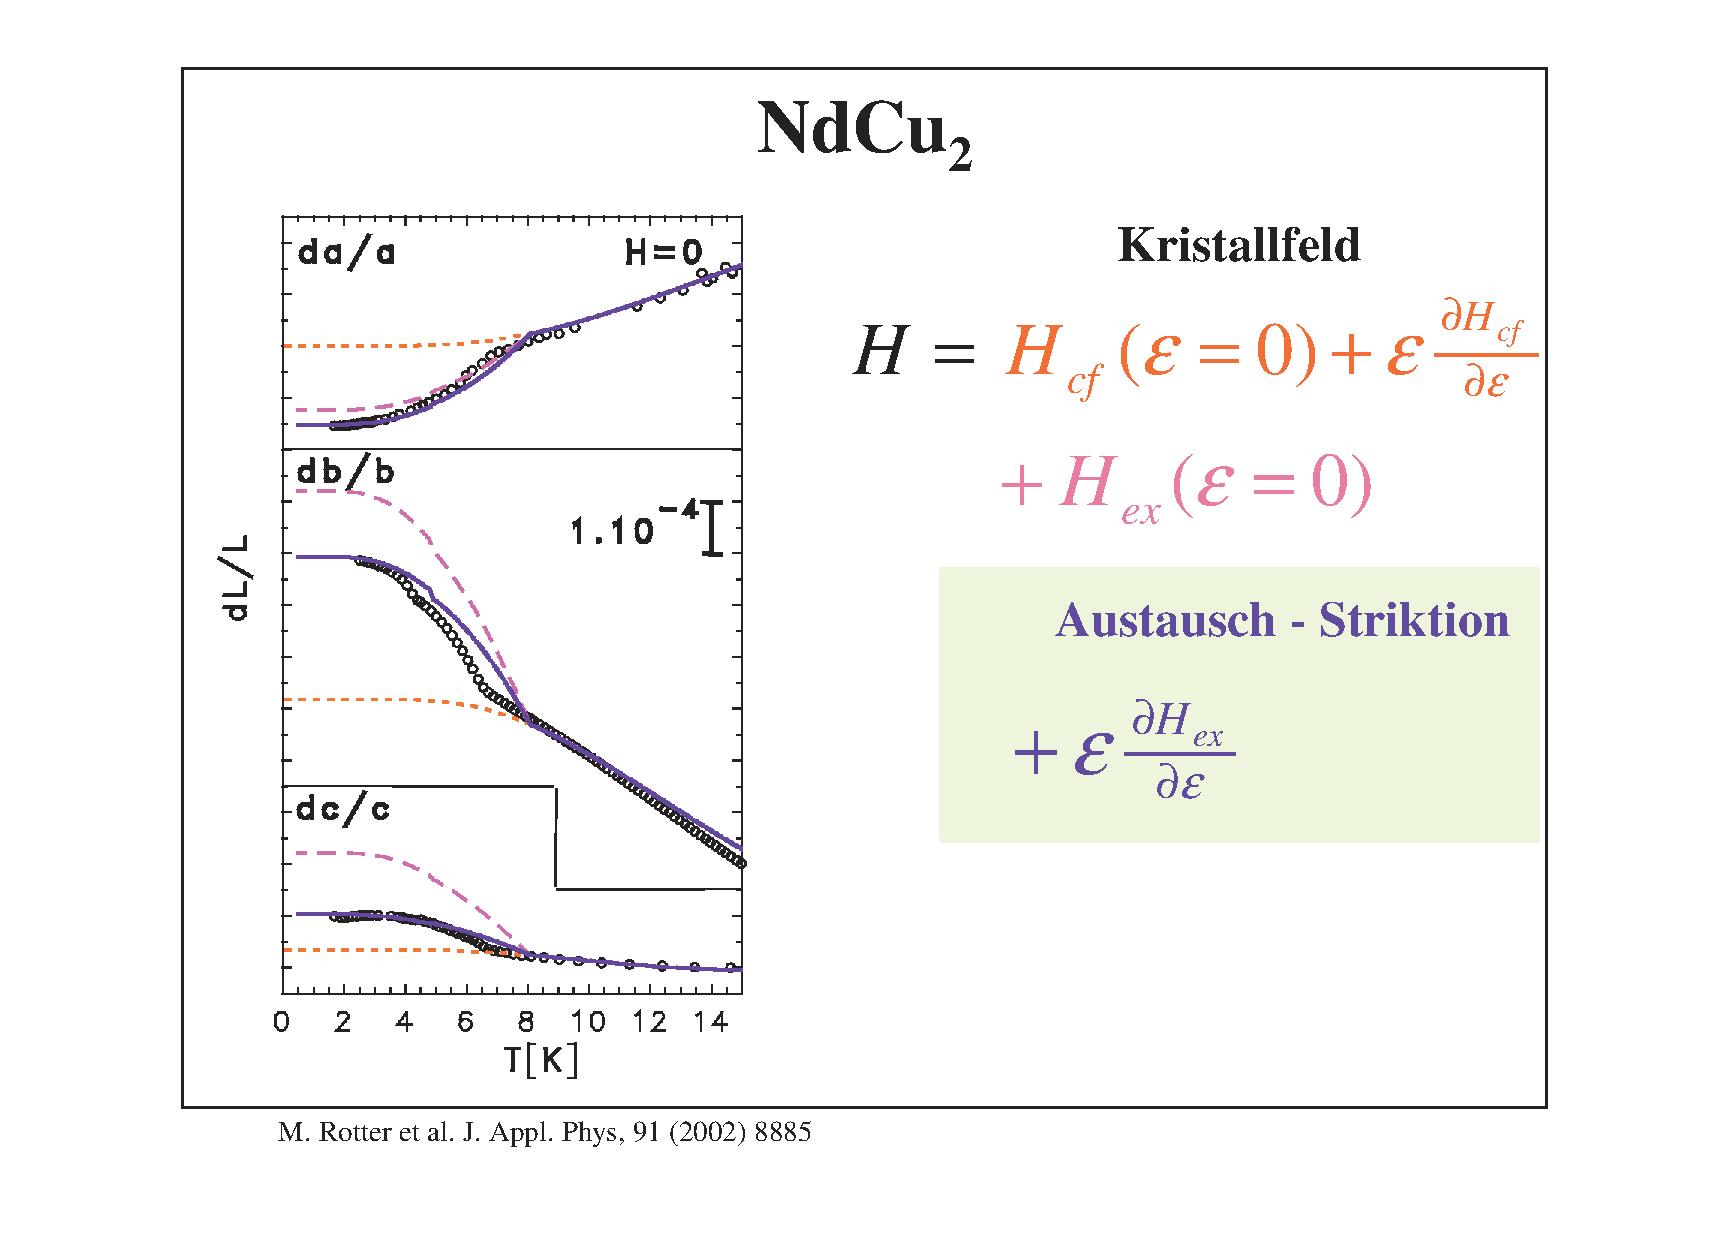
\includegraphics[angle=0, width=0.8\textwidth]{figsrc/magnetostriction_ndcu2.eps}
\end{center}
\caption{Calculated spontaneous magnetostriction of NdCu$_2$.}
\label{magnetostrictiongraphic}
\end{figure}

\begin{description}
\item [\prg mcphas.qvc]    the set of test q-vectors used for calculation of free energy.
                           Components of these q vectors refer to the reciprocal lattice $\vec a^*,\vec b^*,\vec c^*$.
\item [\prg mcphas.phs]    spin-configuration table of different types of spin-configurations. 
                            Note, in case of non-orthogonal axes the convention in these tables 
                            is $mb||\vec b$, $mc||(\vec a \times \vec b)$ and $ma$ perpendicular to $mb$ and $mc$.

                           {\em Note}: 
                           there is no natural criteria for deciding, if one spin-configuration is
			   different from another one. Therefore the list of ''different''
			   spin-configurations is dependent on the meaning of ''different''.
			   
			   The program {\prg McPhase} decides whether a spin-configuration is
			   different from another by a simple criteria, namely by the
			   angle between the spins. Comparing two spin configurations it calculates
			   the angle between corresponding spins and if for one spin the
			   angle is not small, the configuration is treated as a different
			   configuration. Therefore for example a ferromagnet with moments
			   in $a$ has a different spin configuration than a ferromagnet with
			   moments in $b$ direction. 
\item [\prg mcphas.sps]    $T-H$ dependence of spin-configuration. The spin configurations stored in this
                           file may be displayed using the program {\prg spins\index{spins}}, an example is given
			   in figure~\ref{spingraphic}.
                            Note, in case of non-orthogonal axes the convention for applied field $Ha, Hb,Hc$ and
                            also for the moment components $ma, mb, mc$ in these tables 
                            is $mb||\vec b$, $mc||(\vec a \times \vec b)$ and $ma$ perpendicular to $mb$ and $mc$.

\item [\prg mcphas.mf]     $T-H$ dependence of exchange field configuration, stored as $g_J \mu_B H_{xc}(i)$(unit is in meV)
                            for i=1,2,...,number of spins in magnetic unit cell.
                            Note, in case of non-orthogonal axes the convention for applied field $Ha, Hb,Hc$ and
                            also for the mean field components in these tables 
                            is $Hb||\vec b$, $Hc||(\vec a \times \vec b)$ and $Ha$ perpendicular to $Hb$ and $Hc$.
\item [\prg mcphas.fum]    free energy, magnetic energy (the derivative with respect to temperature gives the specific %%@
heat),
                           magnetisation data and (if cfield is used with higher order interactions)
                           expectation values of the Stevens Operators $<O_l^m>$ . As an example for the information
			   contained in this file the calculated magnetisation and magnetostriction of NdCu$_2$ is shown in
			   figures~\ref{magnetization} and ~\ref{magnetizationgraphic}.
                            Note, in case of non-orthogonal axes the convention for applied field $Ha, Hb,Hc$ and
                            also for the magnetisation components $ma,mb,mc$ in these tables 
                            is $Hb||\vec b$, $Hc||(\vec a \times \vec b)$ and $Ha$ perpendicular to $Hb$ and $Hc$.

\item [\prg mcphas1.j1 .j1 .j2 ...] 
               spin-spin correlation functions for sub-lattice 1 neighbour 1 2 ...
	       (linear combination is proportional to magnetostriction)
	       The spin-spin correlation functions for neighbour $k$ are defined by
	       the following sum of dyadic products:

	       \begin{equation}
	        \frac{1}{n}\sum_{s=1}^n <{\mbf J}^s> \times  <{\mbf J}^{s+k}>
	       \end{equation}
	       with $n$ being the number of moments in the magnetic unit cell.
	       Single ion and two-ion magnetostriction can be calculated using the $<O_l^m>$ and the
	       spin-spin correlation functions. As an example the magnetostriction analysis of
	       NdCu$_2$ is shown in figure~\ref{magnetostrictiongraphic}. For details 
             please refer to~\cite{rotter02-8885}.
                            Note, in case of non-orthogonal axes the convention for applied field $Ha, Hb,Hc$ and
                            also for the moment components in these tables 
                            is $Hb||\vec b$, $Hc||(\vec a \times \vec b)$ and $Ha$ perpendicular to $Hb$ and $Hc$.
\item [\prg mcphas.xyt]    phase diagram as x,y,T, H, phase-number j according to spin-configuration table
               given in mcphas.phs, a periodicity key, nettomoments <J>.
 Figure~\ref{phasediagramgraphic}
	       shows the phase diagram of NdCu$_2$ for magnetic fields parallel to the orthorhombic $b$-direction.
                            Note, in case of non-orthogonal axes the convention for applied field $Ha, Hb,Hc$ 
                             in these tables 
                            is $Hb||\vec b$, $Hc||(\vec a \times \vec b)$ and $Ha$ perpendicular to $Hb$ and $Hc$.
\item [\prg mcphas.hkl]    calculated (unpolarised) neutron diffraction data (the calculated magnetic intensities
    correspond to the magnetic structure + Polarisation factor. The
    Lorentz-factor , magnetic form factor and  instrumental corrections are not calculated.)
 As an example figure~\ref{neutintgraphic}
    shows the calculated temperature dependence of magnetic amplitudes for NdCu$_2$.
                           $h,k,l$ refer to the reciprocal lattice $\vec a^*,\vec b^*,\vec c^*$.
                            Note, in case of non-orthogonal axes the convention for applied field $Ha, Hb,Hc$ 
                             in these tables 
                            is $Hb||\vec b$, $Hc||(\vec a \times \vec b)$ and $Ha$ perpendicular to $Hb$ and $Hc$.
    
\item [\prg mcphasa.hkl]    Fourier Transform of the $a$-component of the magnetic Moments.
                           $h,k,l$ refer to the reciprocal lattice $\vec a^*,\vec b^*,\vec c^*$.
                            Note, in case of non-orthogonal axes the convention for applied field $Ha, Hb,Hc$ and
                            the magnetic moment component in these tables 
                            is $Hb||\vec b$, $Hc||(\vec a \times \vec b)$ and $Ha$ perpendicular to $Hb$ and $Hc$.
\item [\prg mcphasb.hkl]    Fourier Transform of the $b$-component of the magnetic Moments.
                           $h,k,l$ refer to the reciprocal lattice $\vec a^*,\vec b^*,\vec c^*$.
                            Note, in case of non-orthogonal axes the convention for applied field $Ha, Hb,Hc$ and
                            the magnetic moment component in these tables 
                            is $Hb||\vec b$, $Hc||(\vec a \times \vec b)$ and $Ha$ perpendicular to $Hb$ and $Hc$.
\item [\prg mcphasc.hkl]    Fourier Transform of the $c$-component of the magnetic Moments.
                           $h,k,l$ refer to the reciprocal lattice $\vec a^*,\vec b^*,\vec c^*$.
                            Note, in case of non-orthogonal axes the convention for applied field $Ha, Hb,Hc$ and
                            the magnetic moment component in these tables 
                            is $Hb||\vec b$, $Hc||(\vec a \times \vec b)$ and $Ha$ perpendicular to $Hb$ and $Hc$.
\end{description} 

\vspace{1cm}
{\em Exercises:}
\begin{itemize}
\item Look at the output files of {\prg McPhase}  in the directory
{\prg examples/ndcu2b\_new/results}.  At which magnetic field
the ferromagnetically aligned state is achieved (at $T=$2~K)?
\item
What is the propagation vector in the different antiferromagnetic phases at $T=$2~K ?
\end{itemize}





\subsubsection{{\prg mcphas.j\index{mcphas.j}} - lattice and exchange parameters}\label{mcphasj}
This file provides the information about 
the crystallographic
 structure and the magnetic exchange interactions.
For every atom in the crystallographic basis there
has to be given the coordinates, the number of neighbours to be considered, the 
Land\'e factor $g_J$, the single ion property filename and  a set of exchange parameters.
If the exchange parameters (and neighbour positions) are not known for your system, you 
can use the program module {\prg makenn\index{makenn}} (see section \ref{addprog}) to generate 
a list of nearest neighbours and
exchange parameters, currently implemented in {\prg makenn\index{makenn}} are dipolar interactions,
exchange interactions via the Bethe-Slater curve or the RKKY model. Note that in order
to use {\prg makenn\index{makenn}} you have to set up a working {\prg mcphas.j\index{mcphas.j}} file, which may or
may not contain neighbours and interactions.

Use program {\prg addj\index{addj}} to add exchange parameter set stored in different 
such {\prg .j} files (see section~\ref{addprog}).



\begin{description}
\item [Line 1,2:] Comment Lines
\item [Line 3:] lattice constants a,b,c and crystal angles alpha, beta, gamma 
\item [Line 4-6:] primitive lattice vectors
\item [Line 7:] Number of atoms in the primitive crystallographic unit cell ({\prg nofatoms})
\item [Line 8:] a comment line with stars
\item [Line 9:] coordinates  ($d_a$,$d_b$,$d_c$) of 1$^{st}$ magnetic ion in the crystallographic unit cell  with
respect to the lattice vectors $\vec a$,$\vec b$,$\vec c$. The number of neighbours of this 
ion, for which interaction constants are given in the interaction table (nofneighbours). 
If {\prg diagonalexchange}
is set to 0 the 9 components of the exchange tensor are given in column 4-12. 
If {\prg diagonalexchange}
 is 1, only 3 components are given (column 4-6).
If {\prg diagonalexchange}
 is 2, specific components of the exchange tensor can be given in columns 4 onwards. The indices of these components
 must be given in the following line (Line 9a below).
The Land\'e factor of the ion (gJ) and the file name of the corresponding single ion
parameter file (cffilename).
\item [Line 9a:]  If {\prg diagonalexchange=2}, then this line gives the indices of the exchange tensor corresponding to 
 the columns 4 onwards. It must have a variable called {\prg indexexchange} followed by a list of names of components of the interaction
 tensor separated by space. E.g.
 \verb|  #! indexexchange= JaJb JbJc  | 
means column 4 gives the the interaction constant between the
 first angular momentum component of the current ion with the second angular momentum component of its neighbour, whilst 
 column 5 has the interaction constant between the second angular momentum component of this ion with the third component of its
 neighbour. Alternatively, pairs of numbers may be given, as in \verb|  #! indexexchange= 1,2 2,3  |
 Additionally another parameter {\prg symmetricexchange} can be set to 1, where the value in each column is also used 
 for the transposed tensor component. Thus \verb|  #! symmetricexchange=1 indexexchange= JaJb  | is the same as \\
 \verb|  #! indexexchange= JaJb JbJa  | where the 4th and 5th column are the same.
\item [Line 10:]  Comment line
\item [Line 11-(10+nofneighbours):] Interaction table for ion number 1.   
Note: the neighbour coordinates (column 1-3) are given with respect to the lattice vectors
$\vec a$,$\vec b$,$\vec c$. The program then calculates from these values the coordinates
with respect to the primitive lattice $\vec r_1$,~$\vec r_2$,~$\vec r_3$.
($ d_a \vec a + d_b \vec b + d_c \vec c = d_1 \vec r_1 + d_2 \vec r_2 + d_3 \vec r_3$).
Column 4,5,6 \dots contain the components of the interaction tensor $\stackrel{=}{\mathcal J}$. 
Note that in case of non-orthogonal axes the 
components of the moments and the interaction tensor $Ja, Jb, Jc, Jaa, Jbb, Jcc, Jab ...$ 
refer to the orthogonal coordinate system
defined with respect to the nonorthogonal lattice $\vec a,\vec b,\vec c$ as
$Jb||\vec b$, $Jc||(\vec a \times \vec b)$ and $Ja$ perpendicular to $Jb$ and $Jc$.
\item [Line (11+nofneighbours) - end:] for each ion in the unit cell line 8 - (10+nofneighbours)
are repeated.
\end{description}


\vspace{0.5cm}

{\small {\bf Information for experienced users:}
\begin{description}
\item[\prg mcphas.jjj:]
format of exchange parameter file, which only needs a reduced set of exchange
parameters in the input file. Using the program {\prg jjj2j} the file can be transformed
to {\prg mcphas.j\index{mcphas.j}} by adding lines for all the equivalent neighbours. The format definition
of {\prg mcphas.jjj} is the same as {\prg mcphas.j\index{mcphas.j}}, however each line denotes several
equivalent neighbour atoms (instead of only one in {\prg mcphas.j\index{mcphas.j}}) according to the
 following rules:
\begin{itemize}
\item If a nonzero coordinate $d_a$ (or $d_b$,$d_c$) in the interaction table
 corresponds to it's value at the nearest
 lattice point of the primitive lattice,
  additional interactions of the same size
with  neighbours with coordinate $-d_a$ (or $-d_b$,$-d_c$, respectively)
are taken into account. This
holds for each of the three coordinates $d_a$,$d_b$ and $d_c$
 resulting in a maximum
number of 8 equivalent neighbours per line in the interaction table.
\item If the value of $d_a$ (or $d_b$,$d_c$) is zero or differs
from it's value at the nearest lattice point of the primitive lattice, it is 
changed to the value at the nearest lattice point and {\bf no} interaction 
with  neighbours with coordinates $-d_a$ (or $-d_b$,$-d_c$) is
 taken into account. If such
 interaction is needed it may be given in a different line and may
have different magnitude. In this way also crystallographic lattices
with no mirror symmetry may be described.
\end{itemize}
\item[\prg mcphas.coq:]   exchange parameters etc [ in old format]...see examples for details, use {\prg coq2jjj} to 
transform {\prg mcphas.coq} to {\prg mcphas.jjj} format
\end{description}

}


\subsubsection{Example {\prg mcphas.j\index{mcphas.j}} file for a simple antiferromagnet}

Here are example files of a tetragonal antiferromagnet with nearest neighbour interactions, all
files are equivalent:

{\small
\begin{verbatim} 
# simple antiferromagnet 
#<!--mcphase.mcphas.j-->
#***************************************************************
# Lattice Constants (A)
#! a=4.3843 b=4.3843 c=2.4194 alpha=  90 beta=  90 gamma=  90
#! r1a=   1 r2a=   0 r3a=   0
#! r1b=   0 r2b=   1 r3b=   0   primitive lattice vectors [a][b][c]
#! r1c=   0 r2c=   0 r3c=   1
#! nofatoms=1  nofcomponents=3  number of atoms in primitive unit cell/number of components of each spin
# ****************************************************************************
#! da=  0 [a] db=  0 [b] dc=  0 nofneighbours=2 diagonalexchange=0 gJ=0.857143 cffilename=Ce3p.sipf
# da[a] db[b] dc[c] Jaa[meV] Jbb[meV] Jcc[meV] Jab[meV] Jba[meV] Jac[meV] Jca[meV] Jbc[meV] Jcb[meV]
+0	+0	+1	-0.1	-0.1	-0.1   0  0  0  0  0  0
+0	+0	-1	-0.1	-0.1	-0.1   0  0  0  0  0  0
#\end{verbatim}
}

Using diagonalexchange this may be shortened to

{\small
\begin{verbatim} 
# simple antiferromagnet 
#<!--mcphase.mcphas.j-->
#***************************************************************
# Lattice Constants (A)
#! a=4.3843 b=4.3843 c=2.4194 alpha=  90 beta=  90 gamma=  90
#! r1a=   1 r2a=   0 r3a=   0
#! r1b=   0 r2b=   1 r3b=   0   primitive lattice vectors [a][b][c]
#! r1c=   0 r2c=   0 r3c=   1
#! nofatoms=1  nofcomponents=3  number of atoms in primitive unit cell/number of components of each spin
# ****************************************************************************
#! da=  0 [a] db=  0 [b] dc=  0 nofneighbours=2 diagonalexchange=1 gJ=0.857143 cffilename=Ce3p.sipf
# da[a] db[b] dc[c] Jaa[meV] Jbb[meV] Jcc[meV] Jab[meV] Jba[meV] Jac[meV] Jca[meV] Jbc[meV] Jcb[meV]
+0	+0	+1	-0.1	-0.1	-0.1   
+0	+0	-1	-0.1	-0.1	-0.1   
#\end{verbatim}
}

with indexexchange option the sequence of two ion interaction parameters can be changed and
zero parameters may be omitted:

{\small
\begin{verbatim} 
# simple antiferromagnet 
#<!--mcphase.mcphas.j-->
#***************************************************************
# Lattice Constants (A)
#! a=4.3843 b=4.3843 c=2.4194 alpha=  90 beta=  90 gamma=  90
#! r1a=   1 r2a=   0 r3a=   0
#! r1b=   0 r2b=   1 r3b=   0   primitive lattice vectors [a][b][c]
#! r1c=   0 r2c=   0 r3c=   1
#! nofatoms=1  nofcomponents=3  number of atoms in primitive unit cell/number of components of each spin
# ****************************************************************************
#! da=  0 [a] db=  0 [b] dc=  0 nofneighbours=2 diagonalexchange=2 gJ=0.857143 cffilename=Ce3p.sipf
# da[a] db[b] dc[c] Jaa[meV] Jbb[meV] Jcc[meV] Jab[meV] Jba[meV] Jac[meV] Jca[meV] Jbc[meV] Jcb[meV]
#! indexexchange = JaJa JaJc JcJa JbJb JcJc
+0	+0	+1	-0.1 0 0 -0.1	-0.1  
+0	+0	-1	-0.1 0 0 -0.1	-0.1  
#\end{verbatim}
}

{\small
\begin{verbatim} 
# simple antiferromagnet 
#<!--mcphase.mcphas.j-->
#***************************************************************
# Lattice Constants (A)
#! a=4.3843 b=4.3843 c=2.4194 alpha=  90 beta=  90 gamma=  90
#! r1a=   1 r2a=   0 r3a=   0
#! r1b=   0 r2b=   1 r3b=   0   primitive lattice vectors [a][b][c]
#! r1c=   0 r2c=   0 r3c=   1
#! nofatoms=1  nofcomponents=3  number of atoms in primitive unit cell/number of components of each spin
# ****************************************************************************
#! da=  0 [a] db=  0 [b] dc=  0 nofneighbours=2 diagonalexchange=2 gJ=0.857143 cffilename=Ce3p.sipf
# da[a] db[b] dc[c] Jaa[meV] Jbb[meV] Jcc[meV] Jab[meV] Jba[meV] Jac[meV] Jca[meV] Jbc[meV] Jcb[meV]
#! indexexchange = 1,1 1,3, 3,1 2,2 3,3
+0	+0	+1	-0.1 0 0 -0.1	-0.1  
+0	+0	-1	-0.1 0 0 -0.1	-0.1  
#\end{verbatim}
}


using symmetricexchange together with indexexchange will assume that the interaction tensor is symmetic and 
only half of it may be given:

{\small
\begin{verbatim} 
# simple antiferromagnet 
#<!--mcphase.mcphas.j-->
#***************************************************************
# Lattice Constants (A)
#! a=4.3843 b=4.3843 c=2.4194 alpha=  90 beta=  90 gamma=  90
#! r1a=   1 r2a=   0 r3a=   0
#! r1b=   0 r2b=   1 r3b=   0   primitive lattice vectors [a][b][c]
#! r1c=   0 r2c=   0 r3c=   1
#! nofatoms=1  nofcomponents=3  number of atoms in primitive unit cell/number of components of each spin
# ****************************************************************************
#! da=  0 [a] db=  0 [b] dc=  0 nofneighbours=2 diagonalexchange=2 gJ=0.857143 cffilename=Ce3p.sipf
# da[a] db[b] dc[c] Jaa[meV] Jbb[meV] Jcc[meV] Jab[meV] Jba[meV] Jac[meV] Jca[meV] Jbc[meV] Jcb[meV]
#! symmetricexchange=1 indexexchange = JaJa JaJc JbJb JcJc
+0	+0	+1	-0.1 0  -0.1	-0.1  
+0	+0	-1	-0.1 0  -0.1	-0.1  
#\end{verbatim}
}


\subsubsection{Single Ion Property Input Files}\label{sifile}

In order to speed up calculations or treat special problems a large 
variety of single ion modules is available. This includes the
option to load a user written single ion module. Details are 
given in chapter~\ref{simod}.

The first time user of {\prg McPhase} should use the module {\prg so1ion}\index{so1ion} and 
create an appropriate single ion property input file as described in
section \ref{cf1ion}. A good starting point are several examples
given in directory {\prg examples}.


\subsubsection{Example single ion property file  for a simple antiferromagnet}

Here is an example file {\prg mcphas.cf1} describing the anisotropy of a 
simple antiferromagnet with Ce atoms having basal plane anisotropy. Note the
axis convention xyz$||$abc, in case of non-orthogonal axes the convention 
is $y||\vec b$, $z||(\vec a \times \vec b)$ and $x$ perpendicular to $y$ and $z$.


\section{{\prg mcphas} - calculation of thermodynamic properties (Magnetisation, Susceptibility, Specific Heat, Neutron %%@
Diffraction, etc.)}
\label{runmcphas}

In order to perform calculations beyond the capabilities of {\prg cfield\index{cfield}} it is necessary
to use the program {\prg mcphas}. 
\begin{itemize}
\item As a first step it is possible to
calculate the thermodynamic properties such as magnetisation or specific heat
considering only single ion effects. In this case all the exchange parameters
have to be set to zero in {\prg mcphas.j\index{mcphas.j}}. 
\item for more advanced calculations the two - ion interactions have to be
considered and may lead to magnetic order. {\prg mcphas} can perform 
calculations in the ordered state in the following way: for 
a given temperature $T$ and magnetic field $\mbf H$ (vector)
several possible magnetic structures are stabilised
by a mean field algorithm and the free energy is 
calculated. The initial values for this mean-field procedure are
modified by a Monte Carlo process.


The temperature and magnetic field is varied during the calculation
and thereby it is possible to map out the magnetic phase diagram.
\end{itemize}

The program produces a plot of the stabilised magnetic
structures and the magnetisation on screen, the
output files contain additional information 
such as calculated magnetoelastic and  neutron-scattering
data. Several graphic programs easy the visualisation of the
calculated data (section~\ref{graphics}).



\subsection{Input Files}
The program {\prg McPhase} needs the following input files (all in the same directory)
 in order to run:

\begin{enumerate}
\item {\prg mcphas.ini\index{mcphas.ini}}
 - controlling the algorithm
\item {\prg mcphas.j\index{mcphas.j}}
  - lattice and exchange parameters
\item {\prg mcphas.tst\index{mcphas.tst}(optional)}  - test spin configurations
\item {\prg single-ion property files}
\item {\prg directory ./results/}
 - directory where calculated data is stored
\item {\prg directory ./fit} - experimental data for fit (optional)
\end{enumerate}


 All
 of these input files have to be in one directory and the program
has to be started in this directory. The results of the simulation
are then stored in the  subdirectory ./results/, which must exist before starting
the program 
... see directory ./examples/ for some examples.
 In order to prepare these files
for a new calculation it is best to take them from an example, copy the files
to a new directory and make the
modifications  to adapt them to the new problem.

\subsubsection{Example - a simple antiferromagnet}

In the following description of the input files we will always refer
to a simple example: a simple antiferromagnet
on a primitive orthorhombic lattice. The first time user
will thus have a simple example to follow, all corresponding
files are given in the directory {\prg tutorial/03magnetic\_phases\_mcphas/simpleAF}.
 

\subsubsection{{\prg mcphas.ini\index{mcphas.ini}} - controlling the algorithm}
   Initial file containing algorithm control parameters, for instance the range and spacing of
   propagation vectors Q or the number of Monte Carlo trials for initial spin configurations
    - {\em mind}: this
   file is rewritten and reread  when running the program and may be changed by the
   user in order to manipulate the running simulation.

{\prg mcphas.ini\index{mcphas.ini}} consists of several sections:
\begin{description}
\item [MCPHASE RUNTIME CONTROL:] this section contains the parameters
controlling the status of the calculation.
\item [XY PHASEDIAGRAM PARAMETERS:] here the temperature and field range and
step widths of the calculation are specified.
The definition of the x and y
axis in terms of temperature and magnetic field is followed by the
corresponding range and step width. An offset may be given for all
field and temperature values.
Note that for most cases of interest
this offset is zero (T0=0, Ha0=0, Hb0=0, Hc0=0).
 For the simple case of calculating a Temperature-Field phase diagram
 It is just necessary to set xT=1 and give the temperature range by
xmin/xmax/xstep. For field in b direction then just set yHb=1 and 
define the range in ymin/ymax/ystep.
In case of non-orthogonal axes the applied magnetic field
components $Ha, Hb, Hc$ refer to the orthogonal coordinate system
defined with respect to the nonorthogonal lattice $\mbf a,\mbf b,\mbf c$ as
$Hb||\mbf b$, $Hc||(\mbf a \times \mbf b)$ and $Ha$ perpendicular to $Hb$ and $Hc$.

\item [GENERATION OF SPINCONFIGURATIONS:] at the beginning of the program
some initial values of spin configurations are generated from a set of 
propagation vectors. This section defines the range of propagation vectors
and the step width.
Depending on the value of the propagation Q with respect to the primitive reciprocal lattice
1-, 2- or 3-dimensional simulations of magnetic lattices
are possible. It is advisable to 
think carefully about the chosen range and spacing of Q vectors in order
to limit calculation time.
 
For example a good starting point is to begin with a calculation with large
step widths (e.g. 0.1)  covering the Brillouin zone. This should give an idea
of the propagation vectors which are stabilised. An advanced calculation
could then fine tune the propagation and determine its accurate value (using
small step widths in a limited area of the zone).
The verbose option of {\prg mcphas} allows to inspect the propagation vectors
which are actually used in the calculation.
Trick: in order to get a quick overview of the
q-vector range covered by the mcphas\index{mcphas} simulation start mcphas, exit and 
just type {\prg felog ./results/mcphas.qvc} (need {\prg perl,perldl,pdl,pgplot} packages).

In order to limit calculation time, the maximum periodicity
of the magnetic unit cell with respect to the crystallographic unit cell 
(maxqperiod) and the maximum number of spins in the magnetic unit cell 
(maxnofspins) can be limited. Also the maximum number of test spin configurations
in the internal table can be limited (maxnoftestspincf).
A critical feature with respect to calculation time is also the number of
spin configurations which are generated by a random process from a tabulated
SPINCONFIGURATIONS during the calculation. 

In summary the variables in this section are mainly important to adapt the
program to a given computer system with finite speed. They have to be set
to optimise between speed and accuracy of the calculation. In order to
find appropriate values it is best to perform some calculations 
and restrict the parameters step by step if insufficient speed is obtained.
Also the examples included in the program package may serve as starting
points.

\item [PARAMETERS FOR SUB FECALC SELFCONSISTENCY PROCESS:] the most important
procedure in the module {\prg mcphas} is the sub fecalc. In this part of the 
program the self consistent calculation of the magnetic moment configuration
is performed as shown schematically in fig.~\ref{fecalc}. 
In the mean field approximation the Hamiltonian~(\ref{hamilton}) is approximated
by

\begin{equation}
 {\mathcal H}=\sum_n H_{SI}^n + E_{corr}
\end{equation}

with the single ion Hamiltonian (in case of module {\prg so1ion\index{so1ion}})

\begin{equation}
H_{SI}^n=  B_l^m O_{lm}({\mbf J}^n) 
	     - g_{Jn} \mu_B {\mbf J}^n {\mbf H^n_{eff}} 
\end{equation}

and the correction term

\begin{equation}
E_{corr}=\frac{1}{2}\sum_{n} g_{Jn} \mu_B \langle {\mbf J}^n
 \rangle (\mbf H^n_{eff}-\mbf H) 
\end{equation}

and with the mean fields $ \mbf H^n_{eff}$ given by

\begin{equation}\label{meanfield}
\mbf H^n_{eff}=\mbf H + \mbf H^n_{xc}=\mbf H+\sum_{{\mbf G'}n'} \frac{{\mathcal J}
(\mbf r_n-(\mbf G'+\mbf r_{n'}))}{g_{Jn}\mu_B } \langle{\mbf
J}^{n'}\rangle
\end{equation}

These mean fields and the moments $\langle \mbf J^n \rangle$ 
are determined in a self consistent
way. For a given magnetic unit cell and initial configuration 
of magnetic moments
the mean fields are calculated according to equation~(\ref{meanfield}). 
Then, for each
magnetic ion the single ion property module is taken 
and the magnetic moment $\langle \mbf J^n \rangle$ is 
calculated from it's mean field. The mean fields are used again in equation~(\ref{meanfield})
and so on .... until convergence is reached. 
Then, the free energy ($f=-kT\sum_n \ln(z_n) + E_{corr}$ ) 
of the stabilised
configuration is calculated (this is why this sub is called {\prg fecalc}). 
The free energies of a lot of different stabilised configurations have to
be compared in order to find out which configuration has lowest free energy, i.e.
is stable in thermal  equilibrium.

It may happen that this process does
not converge due to bad choice of the initial configuration, therefore a maximum number
of mean field loops has to be given by the user.
The results of a calculation may be significantly influenced by
changing parameters such as the maximum number of iteration loops 
in this section. 
In fact the simulation is always a compromise of calculation time and accuracy: if only
a few initial spin configurations are tried at each (H-T) point, the calculation speed is
fast, however it is possible that the program misses the magnetic structure with the
lowest free energy. The same holds if other critical parameters of the simulation are
restricted too much.
 

\item [OUTPUT OF PHYSICAL PROPERTIES:]
Some options for the output of the calculation can be changed in this section.
\end{description}

\begin{figure}[hb]
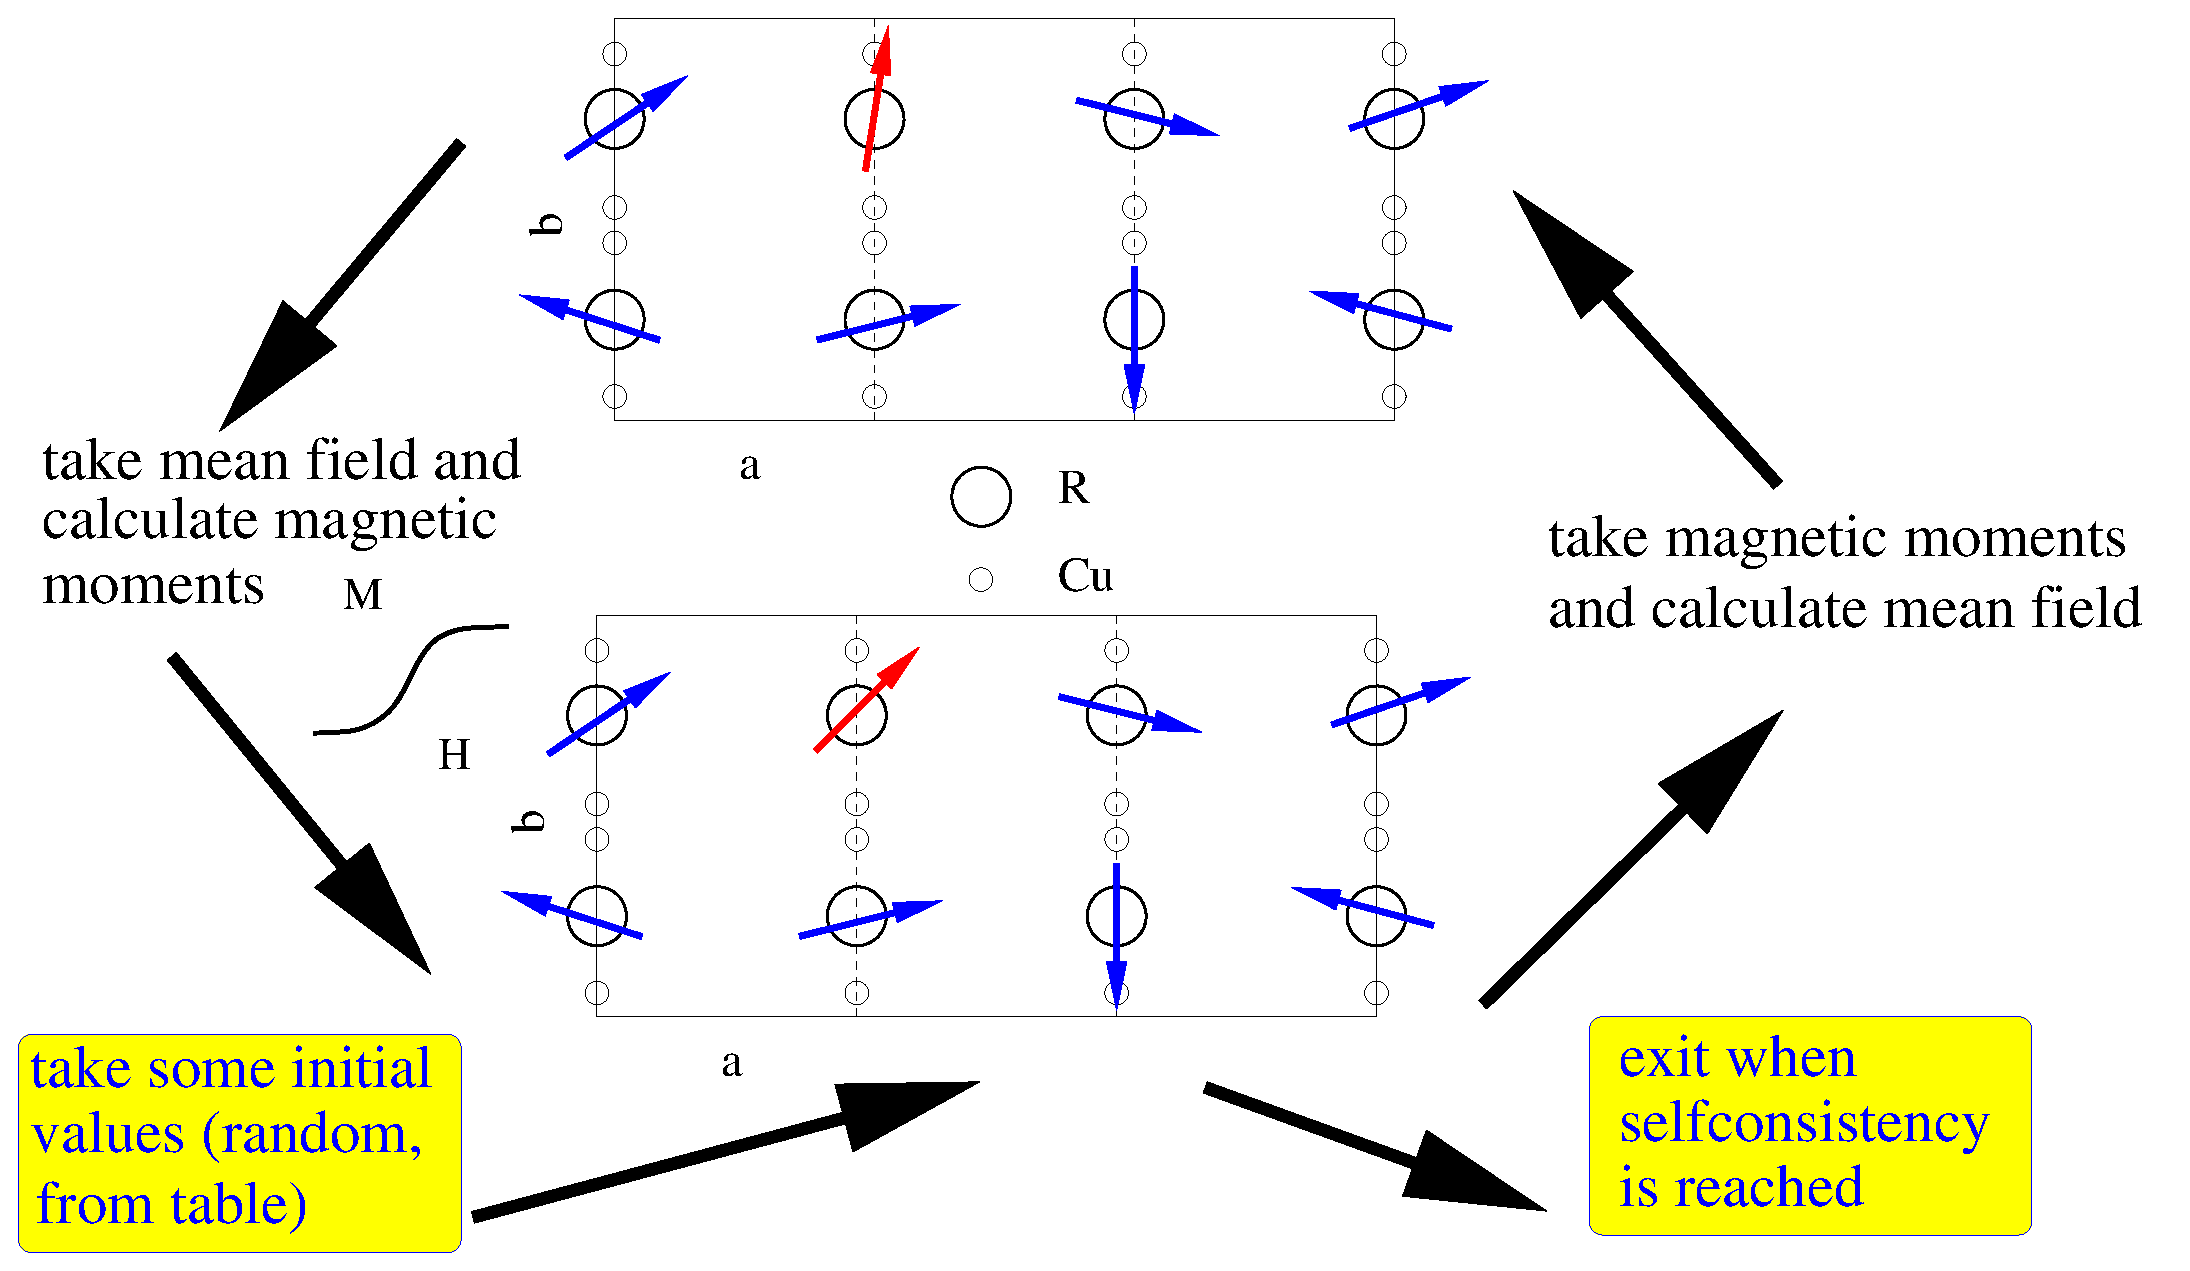
\includegraphics[angle=0,width=0.9\columnwidth]{figsrc/fecalc.eps}
\caption{\label{fecalc}Mean field process of sub {\prg fecalc}.}
\end{figure}

 
\subsubsection{Example {\prg mcphas.ini\index{mcphas.ini}} file for a simple antiferromagnet}

Here is an example of {\prg mcphas.ini\index{mcphas.ini}}, the comments describe the meaning of the different
parameters:

\input{mcphas.ini}



\subsubsection{{\prg mcphas.j\index{mcphas.j}} - lattice and exchange parameters}\label{mcphasj}
This file provides the information about 
the crystallographic
 structure and the magnetic exchange interactions.
For every atom in the crystallographic basis there
has to be given the coordinates, the number of neighbours to be considered, the 
Land\'e factor $g_J$, the single ion property filename and  a set of exchange parameters.
If the exchange parameters (and neighbour positions) are not known for your system, you 
can use the program module {\prg makenn\index{makenn}} (see section \ref{addprog}) to generate 
a list of nearest neighbours and
exchange parameters, currently implemented in {\prg makenn\index{makenn}} are dipolar interactions,
exchange interactions via the Bethe-Slater curve or the RKKY model. Note that in order
to use {\prg makenn\index{makenn}} you have to set up a working {\prg mcphas.j\index{mcphas.j}} file, which may or
may not contain neighbours and interactions.

Use program {\prg addj\index{addj}} to add exchange parameter set stored in different 
such {\prg .j} files (see section~\ref{addprog}).



\begin{description}
\item [Line 1,2:] Comment Lines
\item [Line 3:] lattice constants a,b,c and crystal angles alpha, beta, gamma 
\item [Line 4-6:] primitive lattice vectors
\item [Line 7:] Number of atoms in the primitive crystallographic unit cell ({\prg nofatoms})
\item [Line 8:] a comment line with stars
\item [Line 9:] coordinates  ($d_a$,$d_b$,$d_c$) of 1$^{st}$ magnetic ion in the crystallographic unit cell  with
respect to the lattice vectors $\vec a$,$\vec b$,$\vec c$. The number of neighbours of this 
ion, for which interaction constants are given in the interaction table (nofneighbours). 
If {\prg diagonalexchange}
is set to 0 the 9 components of the exchange tensor are given in column 4-12. 
If {\prg diagonalexchange}
 is 1, only 3 components are given (column 4-6).
If {\prg diagonalexchange}
 is 2, specific components of the exchange tensor can be given in columns 4 onwards. The indices of these components
 must be given in the following line (Line 9a below).
The Land\'e factor of the ion (gJ) and the file name of the corresponding single ion
parameter file (cffilename).
\item [Line 9a:]  If {\prg diagonalexchange=2}, then this line gives the indices of the exchange tensor corresponding to 
 the columns 4 onwards. It must have a variable called {\prg indexexchange} followed by a list of names of components of the interaction
 tensor separated by space. E.g.
 \verb|  #! indexexchange= JaJb JbJc  | 
means column 4 gives the the interaction constant between the
 first angular momentum component of the current ion with the second angular momentum component of its neighbour, whilst 
 column 5 has the interaction constant between the second angular momentum component of this ion with the third component of its
 neighbour. Alternatively, pairs of numbers may be given, as in \verb|  #! indexexchange= 1,2 2,3  |
 Additionally another parameter {\prg symmetricexchange} can be set to 1, where the value in each column is also used 
 for the transposed tensor component. Thus \verb|  #! symmetricexchange=1 indexexchange= JaJb  | is the same as \\
 \verb|  #! indexexchange= JaJb JbJa  | where the 4th and 5th column are the same.
\item [Line 10:]  Comment line
\item [Line 11-(10+nofneighbours):] Interaction table for ion number 1.   
Note: the neighbour coordinates (column 1-3) are given with respect to the lattice vectors
$\vec a$,$\vec b$,$\vec c$. The program then calculates from these values the coordinates
with respect to the primitive lattice $\vec r_1$,~$\vec r_2$,~$\vec r_3$.
($ d_a \vec a + d_b \vec b + d_c \vec c = d_1 \vec r_1 + d_2 \vec r_2 + d_3 \vec r_3$).
Column 4,5,6 \dots contain the components of the interaction tensor $\stackrel{=}{\mathcal J}$. 
Note that in case of non-orthogonal axes the 
components of the moments and the interaction tensor $Ja, Jb, Jc, Jaa, Jbb, Jcc, Jab ...$ 
refer to the orthogonal coordinate system
defined with respect to the nonorthogonal lattice $\vec a,\vec b,\vec c$ as
$Jb||\vec b$, $Jc||(\vec a \times \vec b)$ and $Ja$ perpendicular to $Jb$ and $Jc$.
\item [Line (11+nofneighbours) - end:] for each ion in the unit cell line 8 - (10+nofneighbours)
are repeated.
\end{description}


\vspace{0.5cm}

{\small {\bf Information for experienced users:}
\begin{description}
\item[\prg mcphas.jjj:]
format of exchange parameter file, which only needs a reduced set of exchange
parameters in the input file. Using the program {\prg jjj2j} the file can be transformed
to {\prg mcphas.j\index{mcphas.j}} by adding lines for all the equivalent neighbours. The format definition
of {\prg mcphas.jjj} is the same as {\prg mcphas.j\index{mcphas.j}}, however each line denotes several
equivalent neighbour atoms (instead of only one in {\prg mcphas.j\index{mcphas.j}}) according to the
 following rules:
\begin{itemize}
\item If a nonzero coordinate $d_a$ (or $d_b$,$d_c$) in the interaction table
 corresponds to it's value at the nearest
 lattice point of the primitive lattice,
  additional interactions of the same size
with  neighbours with coordinate $-d_a$ (or $-d_b$,$-d_c$, respectively)
are taken into account. This
holds for each of the three coordinates $d_a$,$d_b$ and $d_c$
 resulting in a maximum
number of 8 equivalent neighbours per line in the interaction table.
\item If the value of $d_a$ (or $d_b$,$d_c$) is zero or differs
from it's value at the nearest lattice point of the primitive lattice, it is 
changed to the value at the nearest lattice point and {\bf no} interaction 
with  neighbours with coordinates $-d_a$ (or $-d_b$,$-d_c$) is
 taken into account. If such
 interaction is needed it may be given in a different line and may
have different magnitude. In this way also crystallographic lattices
with no mirror symmetry may be described.
\end{itemize}
\item[\prg mcphas.coq:]   exchange parameters etc [ in old format]...see examples for details, use {\prg coq2jjj} to 
transform {\prg mcphas.coq} to {\prg mcphas.jjj} format
\end{description}

}


\subsubsection{Example {\prg mcphas.j\index{mcphas.j}} file for a simple antiferromagnet}

Here are example files of a tetragonal antiferromagnet with nearest neighbour interactions, all
files are equivalent:

{\small
\begin{verbatim} 
# simple antiferromagnet 
#<!--mcphase.mcphas.j-->
#***************************************************************
# Lattice Constants (A)
#! a=4.3843 b=4.3843 c=2.4194 alpha=  90 beta=  90 gamma=  90
#! r1a=   1 r2a=   0 r3a=   0
#! r1b=   0 r2b=   1 r3b=   0   primitive lattice vectors [a][b][c]
#! r1c=   0 r2c=   0 r3c=   1
#! nofatoms=1  nofcomponents=3  number of atoms in primitive unit cell/number of components of each spin
# ****************************************************************************
#! da=  0 [a] db=  0 [b] dc=  0 nofneighbours=2 diagonalexchange=0 gJ=0.857143 cffilename=Ce3p.sipf
# da[a] db[b] dc[c] Jaa[meV] Jbb[meV] Jcc[meV] Jab[meV] Jba[meV] Jac[meV] Jca[meV] Jbc[meV] Jcb[meV]
+0	+0	+1	-0.1	-0.1	-0.1   0  0  0  0  0  0
+0	+0	-1	-0.1	-0.1	-0.1   0  0  0  0  0  0
#\end{verbatim}
}

Using diagonalexchange this may be shortened to

{\small
\begin{verbatim} 
# simple antiferromagnet 
#<!--mcphase.mcphas.j-->
#***************************************************************
# Lattice Constants (A)
#! a=4.3843 b=4.3843 c=2.4194 alpha=  90 beta=  90 gamma=  90
#! r1a=   1 r2a=   0 r3a=   0
#! r1b=   0 r2b=   1 r3b=   0   primitive lattice vectors [a][b][c]
#! r1c=   0 r2c=   0 r3c=   1
#! nofatoms=1  nofcomponents=3  number of atoms in primitive unit cell/number of components of each spin
# ****************************************************************************
#! da=  0 [a] db=  0 [b] dc=  0 nofneighbours=2 diagonalexchange=1 gJ=0.857143 cffilename=Ce3p.sipf
# da[a] db[b] dc[c] Jaa[meV] Jbb[meV] Jcc[meV] Jab[meV] Jba[meV] Jac[meV] Jca[meV] Jbc[meV] Jcb[meV]
+0	+0	+1	-0.1	-0.1	-0.1   
+0	+0	-1	-0.1	-0.1	-0.1   
#\end{verbatim}
}

with indexexchange option the sequence of two ion interaction parameters can be changed and
zero parameters may be omitted:

{\small
\begin{verbatim} 
# simple antiferromagnet 
#<!--mcphase.mcphas.j-->
#***************************************************************
# Lattice Constants (A)
#! a=4.3843 b=4.3843 c=2.4194 alpha=  90 beta=  90 gamma=  90
#! r1a=   1 r2a=   0 r3a=   0
#! r1b=   0 r2b=   1 r3b=   0   primitive lattice vectors [a][b][c]
#! r1c=   0 r2c=   0 r3c=   1
#! nofatoms=1  nofcomponents=3  number of atoms in primitive unit cell/number of components of each spin
# ****************************************************************************
#! da=  0 [a] db=  0 [b] dc=  0 nofneighbours=2 diagonalexchange=2 gJ=0.857143 cffilename=Ce3p.sipf
# da[a] db[b] dc[c] Jaa[meV] Jbb[meV] Jcc[meV] Jab[meV] Jba[meV] Jac[meV] Jca[meV] Jbc[meV] Jcb[meV]
#! indexexchange = JaJa JaJc JcJa JbJb JcJc
+0	+0	+1	-0.1 0 0 -0.1	-0.1  
+0	+0	-1	-0.1 0 0 -0.1	-0.1  
#\end{verbatim}
}

{\small
\begin{verbatim} 
# simple antiferromagnet 
#<!--mcphase.mcphas.j-->
#***************************************************************
# Lattice Constants (A)
#! a=4.3843 b=4.3843 c=2.4194 alpha=  90 beta=  90 gamma=  90
#! r1a=   1 r2a=   0 r3a=   0
#! r1b=   0 r2b=   1 r3b=   0   primitive lattice vectors [a][b][c]
#! r1c=   0 r2c=   0 r3c=   1
#! nofatoms=1  nofcomponents=3  number of atoms in primitive unit cell/number of components of each spin
# ****************************************************************************
#! da=  0 [a] db=  0 [b] dc=  0 nofneighbours=2 diagonalexchange=2 gJ=0.857143 cffilename=Ce3p.sipf
# da[a] db[b] dc[c] Jaa[meV] Jbb[meV] Jcc[meV] Jab[meV] Jba[meV] Jac[meV] Jca[meV] Jbc[meV] Jcb[meV]
#! indexexchange = 1,1 1,3, 3,1 2,2 3,3
+0	+0	+1	-0.1 0 0 -0.1	-0.1  
+0	+0	-1	-0.1 0 0 -0.1	-0.1  
#\end{verbatim}
}


using symmetricexchange together with indexexchange will assume that the interaction tensor is symmetic and 
only half of it may be given:

{\small
\begin{verbatim} 
# simple antiferromagnet 
#<!--mcphase.mcphas.j-->
#***************************************************************
# Lattice Constants (A)
#! a=4.3843 b=4.3843 c=2.4194 alpha=  90 beta=  90 gamma=  90
#! r1a=   1 r2a=   0 r3a=   0
#! r1b=   0 r2b=   1 r3b=   0   primitive lattice vectors [a][b][c]
#! r1c=   0 r2c=   0 r3c=   1
#! nofatoms=1  nofcomponents=3  number of atoms in primitive unit cell/number of components of each spin
# ****************************************************************************
#! da=  0 [a] db=  0 [b] dc=  0 nofneighbours=2 diagonalexchange=2 gJ=0.857143 cffilename=Ce3p.sipf
# da[a] db[b] dc[c] Jaa[meV] Jbb[meV] Jcc[meV] Jab[meV] Jba[meV] Jac[meV] Jca[meV] Jbc[meV] Jcb[meV]
#! symmetricexchange=1 indexexchange = JaJa JaJc JbJb JcJc
+0	+0	+1	-0.1 0  -0.1	-0.1  
+0	+0	-1	-0.1 0  -0.1	-0.1  
#\end{verbatim}
}


\subsubsection{Single Ion Property Input Files}\label{sifile}

In order to speed up calculations or treat special problems a large 
variety of single ion modules is available. This includes the
option to load a user written single ion module. Details are 
given in chapter~\ref{simod}.

The first time user of {\prg McPhase} should use the module {\prg so1ion}\index{so1ion} and 
create an appropriate single ion property input file as described in
section \ref{cf1ion}. A good starting point are several examples
given in directory {\prg examples}.


\subsubsection{Example single ion property file  for a simple antiferromagnet}

Here is an example file {\prg mcphas.cf1} describing the anisotropy of a 
simple antiferromagnet with Ce atoms having basal plane anisotropy. Note the
axis convention xyz$||$abc, in case of non-orthogonal axes the convention 
is $y||\vec b$, $z||(\vec a \times \vec b)$ and $x$ perpendicular to $y$ and $z$.


\input{mcphas.cf1}

\subsubsection{{\prg mcphas.tst\index{mcphas.tst}} - input file of test spin-configurations (optional)}
This file is optional and contains
some test momentum configurations to be used for the calculation
             of the free energy. Mind that
\begin{itemize}
\item  in the file header the number of atoms in the primitive
       crystallographic unit cell and the number of components
       of the spin vector have to be given.
\item  at the end of the
 file there must be no empty lines !
\end{itemize}

The momentum - configurations tables always refer to spins sitting on
the primitive lattice ${\mbf r}_i$. If more than one atom is in
the primitive basis, the momentum gets $3n$ components ($n=$ number
of atoms in the crystallographic basis). See {\prg ./examples/ndcu2b\_new/} for
examples of a two atom basis. Units of these tables are that of total 
angular momentum $<J>$.

\subsubsection{Example {\prg mcphas.tst\index{mcphas.tst}} file  for a simple antiferromagnet}

Here is the file {\prg mcphas.tst\index{mcphas.tst}} for the simple antiferromagnet example
describing some spin configurations
to be used as starting values for the mean field process:

\input{mcphas.tst}
Note, in case of non-orthogonal axes the convention 
is $mb||\vec b$, $mc||(\vec a \times \vec b)$ and $ma$ perpendicular to $mb$ and $mc$.

\subsubsection{subdirectory {\prg ./results} - directory where calculated data is stored}

In order to be able to save the results of a calculation the directory {\prg ./results} has to
exist. Mind that all files in this directory will be overwritten without warning. 

\subsubsection{subdirectory {\prg ./fit} - experimental data for fit (optional) } 

In order that {\prg McPhase} can calculate the standard deviation between
 experimental data and the results of the simulation, some experimental data
 can be given in the subdirectory {\prg ./fit}. The filenames and the data-format
 are the same as the output files of {\prg McPhas}, e.g. {\prg mcphas.fum}, {\prg mcphas.hkl}
 etc. {\prg McPhase} looks into the directory {\prg ./fit} and if it finds any
 of these files, the standard deviation is increased correspondingly. 

What measurement data can be used to calculate a standard deviation ?

\begin{description}
\item[{\prg mcphas.fum}] if given in column 11, 12, 13 in {\prg ./fit/mcphas.fum} the
            magnetisation in the $a$, $b$ and $c$ direction is used for calculation
	    of the standard deviation sta. The standard deviation is calculated
	    as ${\rm sta}=\sum_{\rm data points i} ({\mbf m}_i^{calc}-{\mbf m}_i^{meas})^2$.
	    All three components of the magnetic moment have to be given and are used.

\end{description}

Note that the measured data has to be given in those (H-T) points which are 
calculated by mcphas\index{mcphas} in order to be used by the program to increase {\prg sta}.
It is usually most effective to fit only few data points, because a large set
of data points will not improve the quality of the fit and only require a large
amount of calculation time.



\subsection{Starting a simulation}
\label{start}

To start the simulation goto the directory containing the
input files {\prg mcphas.ini, mcphas.j, etc. } and type

\begin{description}
\item[\prg mcphas] to run the program generating stepwise $H-T$ values 
              in a loop given by {\prg mcphas.ini\index{mcphas.ini}} (you can also press the
              symbol in the {\prg McPhase - Explorer} window).
\item[\prg mcphas\index{mcphas} [file]]  to run the program with an input file --   
             {\prg file} contains T ha hb hc values to be calculated 
             if [file] is not given, xmin xmax xstep (xT xHa xHb xHc)
             ymin ymax ystep (yT yHa yHb yHc) is read from file {\prg mcphas.ini\index{mcphas.ini}}
	     and phase diagram is calculated
\item[\prg mcphas\index{mcphas} -h]  to  print help and version of {\prg McPhas}.
\item[\prg mcphas\index{mcphas} -stamax 14]  end mcphas\index{mcphas} if standard deviation exceeds 14.
\item[\prg mcphas\index{mcphas} -a] avoid overwriting output files in results, append new results to existing files
\item[\prg mcphas\index{mcphas} -v]  to  enable verbose mode with lots of messages of {\prg McPhas}. Specifically
the verbose mode enables the following features:
  \begin{itemize}
			          \item more information is printed out, 
			          \item the q-vectors file {\prg ./results/mcphas.qvc} will contain 
				    the explicit spin configurations
			          \item the display\index{display} on screen (ghostview window using 
				     {\prg ./results/.sps.eps}) will be updated not only 
				    when a H-T point has been finished but always 
				    when a structure with smaller free energy 
				    has been stabilised
  \end{itemize}
\item[\prg mcphasit\index{mcphas}] to start mcphase in commandline mode without opening any window
\end{description}

\vspace{1cm}
{\em Exercises:}
\begin{itemize}
\item Look at the input files for {\prg McPhase} given in the directory
{\prg examples/ndcu2b\_new}.  How many atoms are contained in the crystallographic basis ?
\item
Start the simulation by typing the command {\prg mcphas}.
\end{itemize}



\subsection{Options for a running simulation}
... when the program is running, the options in the main window
can be changed. Pressing ''displayall'' displays the current spin-configuration
at each iteration step. Pressing ''log fe vs Q'' appends free energy vs Q
data to {\prg mcphas.log} for every ($T-H$) point.


The file {\prg ./results/.spins.eps} is used to show the information about the currently calculated
spin structure on the screen using the postscript file viewer ghostview.

The file {\prg ./results/.mcphas.fum} contains the information of the magnetisation curve
which is currently calculated. This information is automatically displayed on the screen.


The program {\prg display} (see section \ref{display}) can be used 
for the online display\index{display} of any other
curve(s).


\subsection{Output Files - {\prg mcphas.qvc,phs,sps,mf,fum,j1...,xyt,hkl} }\label{outputfiles}
 (in directory ./results/ after a simulation run) 

\begin{figure}[htb]%h=here, t=top, b=bottom, p=separate figure page
\begin{center}\leavevmode
\includegraphics[angle=0, width=0.3\textwidth]{figsrc/magnetization_ndcu2.ps}
\end{center}
\caption{Calculated magnetisation of NdCu$_2$ for field parallel to the orthorhombic $b$-direction.}
\label{magnetization}
\end{figure}

\begin{figure}[htb]%h=here, t=top, b=bottom, p=separate figure page
\begin{center}\leavevmode
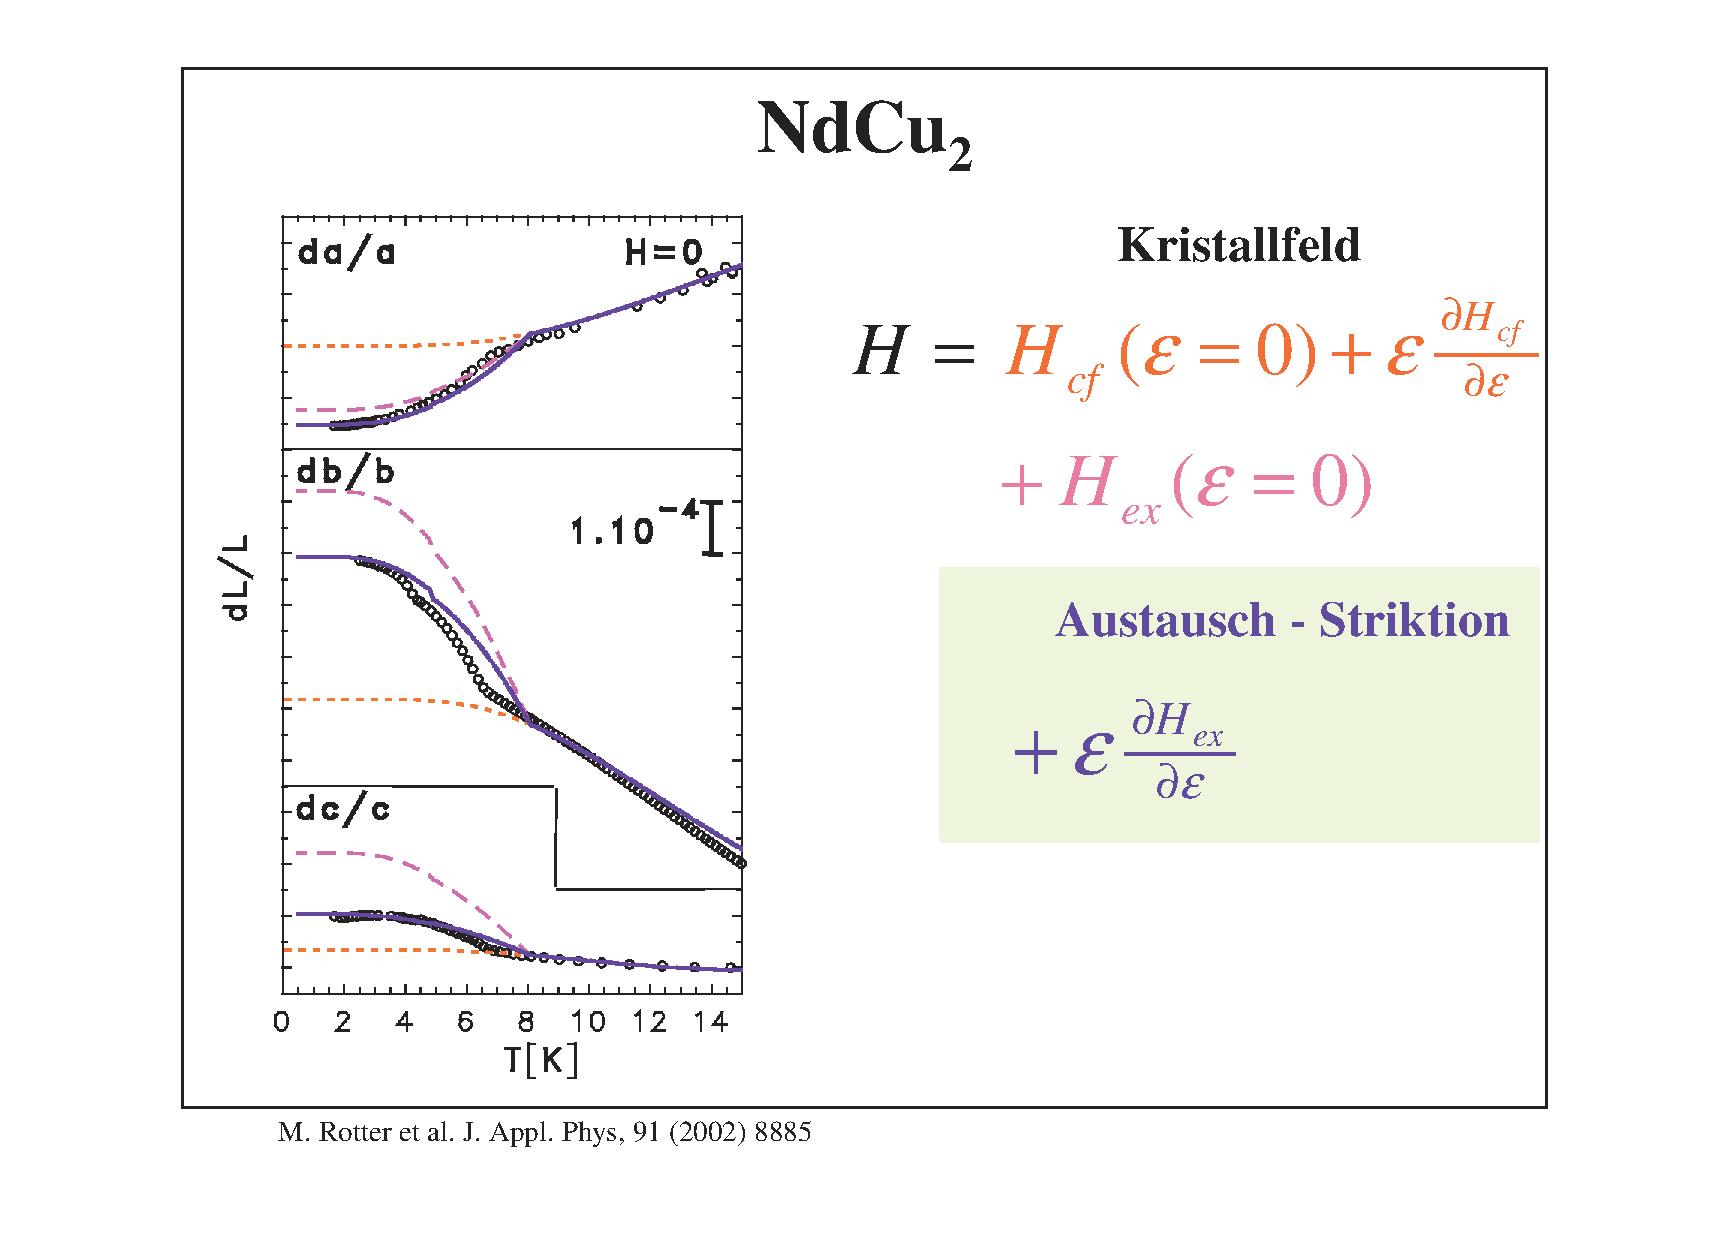
\includegraphics[angle=0, width=0.8\textwidth]{figsrc/magnetostriction_ndcu2.eps}
\end{center}
\caption{Calculated spontaneous magnetostriction of NdCu$_2$.}
\label{magnetostrictiongraphic}
\end{figure}

\begin{description}
\item [\prg mcphas.qvc]    the set of test q-vectors used for calculation of free energy.
                           Components of these q vectors refer to the reciprocal lattice $\vec a^*,\vec b^*,\vec c^*$.
\item [\prg mcphas.phs]    spin-configuration table of different types of spin-configurations. 
                            Note, in case of non-orthogonal axes the convention in these tables 
                            is $mb||\vec b$, $mc||(\vec a \times \vec b)$ and $ma$ perpendicular to $mb$ and $mc$.

                           {\em Note}: 
                           there is no natural criteria for deciding, if one spin-configuration is
			   different from another one. Therefore the list of ''different''
			   spin-configurations is dependent on the meaning of ''different''.
			   
			   The program {\prg McPhase} decides whether a spin-configuration is
			   different from another by a simple criteria, namely by the
			   angle between the spins. Comparing two spin configurations it calculates
			   the angle between corresponding spins and if for one spin the
			   angle is not small, the configuration is treated as a different
			   configuration. Therefore for example a ferromagnet with moments
			   in $a$ has a different spin configuration than a ferromagnet with
			   moments in $b$ direction. 
\item [\prg mcphas.sps]    $T-H$ dependence of spin-configuration. The spin configurations stored in this
                           file may be displayed using the program {\prg spins\index{spins}}, an example is given
			   in figure~\ref{spingraphic}.
                            Note, in case of non-orthogonal axes the convention for applied field $Ha, Hb,Hc$ and
                            also for the moment components $ma, mb, mc$ in these tables 
                            is $mb||\vec b$, $mc||(\vec a \times \vec b)$ and $ma$ perpendicular to $mb$ and $mc$.

\item [\prg mcphas.mf]     $T-H$ dependence of exchange field configuration, stored as $g_J \mu_B H_{xc}(i)$(unit is in meV)
                            for i=1,2,...,number of spins in magnetic unit cell.
                            Note, in case of non-orthogonal axes the convention for applied field $Ha, Hb,Hc$ and
                            also for the mean field components in these tables 
                            is $Hb||\vec b$, $Hc||(\vec a \times \vec b)$ and $Ha$ perpendicular to $Hb$ and $Hc$.
\item [\prg mcphas.fum]    free energy, magnetic energy (the derivative with respect to temperature gives the specific %%@
heat),
                           magnetisation data and (if cfield is used with higher order interactions)
                           expectation values of the Stevens Operators $<O_l^m>$ . As an example for the information
			   contained in this file the calculated magnetisation and magnetostriction of NdCu$_2$ is shown in
			   figures~\ref{magnetization} and ~\ref{magnetizationgraphic}.
                            Note, in case of non-orthogonal axes the convention for applied field $Ha, Hb,Hc$ and
                            also for the magnetisation components $ma,mb,mc$ in these tables 
                            is $Hb||\vec b$, $Hc||(\vec a \times \vec b)$ and $Ha$ perpendicular to $Hb$ and $Hc$.

\item [\prg mcphas1.j1 .j1 .j2 ...] 
               spin-spin correlation functions for sub-lattice 1 neighbour 1 2 ...
	       (linear combination is proportional to magnetostriction)
	       The spin-spin correlation functions for neighbour $k$ are defined by
	       the following sum of dyadic products:

	       \begin{equation}
	        \frac{1}{n}\sum_{s=1}^n <{\mbf J}^s> \times  <{\mbf J}^{s+k}>
	       \end{equation}
	       with $n$ being the number of moments in the magnetic unit cell.
	       Single ion and two-ion magnetostriction can be calculated using the $<O_l^m>$ and the
	       spin-spin correlation functions. As an example the magnetostriction analysis of
	       NdCu$_2$ is shown in figure~\ref{magnetostrictiongraphic}. For details 
             please refer to~\cite{rotter02-8885}.
                            Note, in case of non-orthogonal axes the convention for applied field $Ha, Hb,Hc$ and
                            also for the moment components in these tables 
                            is $Hb||\vec b$, $Hc||(\vec a \times \vec b)$ and $Ha$ perpendicular to $Hb$ and $Hc$.
\item [\prg mcphas.xyt]    phase diagram as x,y,T, H, phase-number j according to spin-configuration table
               given in mcphas.phs, a periodicity key, nettomoments <J>.
 Figure~\ref{phasediagramgraphic}
	       shows the phase diagram of NdCu$_2$ for magnetic fields parallel to the orthorhombic $b$-direction.
                            Note, in case of non-orthogonal axes the convention for applied field $Ha, Hb,Hc$ 
                             in these tables 
                            is $Hb||\vec b$, $Hc||(\vec a \times \vec b)$ and $Ha$ perpendicular to $Hb$ and $Hc$.
\item [\prg mcphas.hkl]    calculated (unpolarised) neutron diffraction data (the calculated magnetic intensities
    correspond to the magnetic structure + Polarisation factor. The
    Lorentz-factor , magnetic form factor and  instrumental corrections are not calculated.)
 As an example figure~\ref{neutintgraphic}
    shows the calculated temperature dependence of magnetic amplitudes for NdCu$_2$.
                           $h,k,l$ refer to the reciprocal lattice $\vec a^*,\vec b^*,\vec c^*$.
                            Note, in case of non-orthogonal axes the convention for applied field $Ha, Hb,Hc$ 
                             in these tables 
                            is $Hb||\vec b$, $Hc||(\vec a \times \vec b)$ and $Ha$ perpendicular to $Hb$ and $Hc$.
    
\item [\prg mcphasa.hkl]    Fourier Transform of the $a$-component of the magnetic Moments.
                           $h,k,l$ refer to the reciprocal lattice $\vec a^*,\vec b^*,\vec c^*$.
                            Note, in case of non-orthogonal axes the convention for applied field $Ha, Hb,Hc$ and
                            the magnetic moment component in these tables 
                            is $Hb||\vec b$, $Hc||(\vec a \times \vec b)$ and $Ha$ perpendicular to $Hb$ and $Hc$.
\item [\prg mcphasb.hkl]    Fourier Transform of the $b$-component of the magnetic Moments.
                           $h,k,l$ refer to the reciprocal lattice $\vec a^*,\vec b^*,\vec c^*$.
                            Note, in case of non-orthogonal axes the convention for applied field $Ha, Hb,Hc$ and
                            the magnetic moment component in these tables 
                            is $Hb||\vec b$, $Hc||(\vec a \times \vec b)$ and $Ha$ perpendicular to $Hb$ and $Hc$.
\item [\prg mcphasc.hkl]    Fourier Transform of the $c$-component of the magnetic Moments.
                           $h,k,l$ refer to the reciprocal lattice $\vec a^*,\vec b^*,\vec c^*$.
                            Note, in case of non-orthogonal axes the convention for applied field $Ha, Hb,Hc$ and
                            the magnetic moment component in these tables 
                            is $Hb||\vec b$, $Hc||(\vec a \times \vec b)$ and $Ha$ perpendicular to $Hb$ and $Hc$.
\end{description} 

\vspace{1cm}
{\em Exercises:}
\begin{itemize}
\item Look at the output files of {\prg McPhase}  in the directory
{\prg examples/ndcu2b\_new/results}.  At which magnetic field
the ferromagnetically aligned state is achieved (at $T=$2~K)?
\item
What is the propagation vector in the different antiferromagnetic phases at $T=$2~K ?
\end{itemize}



\subsubsection{{\prg mcphas.tst\index{mcphas.tst}} - input file of test spin-configurations (optional)}
This file is optional and contains
some test momentum configurations to be used for the calculation
             of the free energy. Mind that
\begin{itemize}
\item  in the file header the number of atoms in the primitive
       crystallographic unit cell and the number of components
       of the spin vector have to be given.
\item  at the end of the
 file there must be no empty lines !
\end{itemize}

The momentum - configurations tables always refer to spins sitting on
the primitive lattice ${\mbf r}_i$. If more than one atom is in
the primitive basis, the momentum gets $3n$ components ($n=$ number
of atoms in the crystallographic basis). See {\prg ./examples/ndcu2b\_new/} for
examples of a two atom basis. Units of these tables are that of total 
angular momentum $<J>$.

\subsubsection{Example {\prg mcphas.tst\index{mcphas.tst}} file  for a simple antiferromagnet}

Here is the file {\prg mcphas.tst\index{mcphas.tst}} for the simple antiferromagnet example
describing some spin configurations
to be used as starting values for the mean field process:

\section{{\prg mcphas} - calculation of thermodynamic properties (Magnetisation, Susceptibility, Specific Heat, Neutron %%@
Diffraction, etc.)}
\label{runmcphas}

In order to perform calculations beyond the capabilities of {\prg cfield\index{cfield}} it is necessary
to use the program {\prg mcphas}. 
\begin{itemize}
\item As a first step it is possible to
calculate the thermodynamic properties such as magnetisation or specific heat
considering only single ion effects. In this case all the exchange parameters
have to be set to zero in {\prg mcphas.j\index{mcphas.j}}. 
\item for more advanced calculations the two - ion interactions have to be
considered and may lead to magnetic order. {\prg mcphas} can perform 
calculations in the ordered state in the following way: for 
a given temperature $T$ and magnetic field $\mbf H$ (vector)
several possible magnetic structures are stabilised
by a mean field algorithm and the free energy is 
calculated. The initial values for this mean-field procedure are
modified by a Monte Carlo process.


The temperature and magnetic field is varied during the calculation
and thereby it is possible to map out the magnetic phase diagram.
\end{itemize}

The program produces a plot of the stabilised magnetic
structures and the magnetisation on screen, the
output files contain additional information 
such as calculated magnetoelastic and  neutron-scattering
data. Several graphic programs easy the visualisation of the
calculated data (section~\ref{graphics}).



\subsection{Input Files}
The program {\prg McPhase} needs the following input files (all in the same directory)
 in order to run:

\begin{enumerate}
\item {\prg mcphas.ini\index{mcphas.ini}}
 - controlling the algorithm
\item {\prg mcphas.j\index{mcphas.j}}
  - lattice and exchange parameters
\item {\prg mcphas.tst\index{mcphas.tst}(optional)}  - test spin configurations
\item {\prg single-ion property files}
\item {\prg directory ./results/}
 - directory where calculated data is stored
\item {\prg directory ./fit} - experimental data for fit (optional)
\end{enumerate}


 All
 of these input files have to be in one directory and the program
has to be started in this directory. The results of the simulation
are then stored in the  subdirectory ./results/, which must exist before starting
the program 
... see directory ./examples/ for some examples.
 In order to prepare these files
for a new calculation it is best to take them from an example, copy the files
to a new directory and make the
modifications  to adapt them to the new problem.

\subsubsection{Example - a simple antiferromagnet}

In the following description of the input files we will always refer
to a simple example: a simple antiferromagnet
on a primitive orthorhombic lattice. The first time user
will thus have a simple example to follow, all corresponding
files are given in the directory {\prg tutorial/03magnetic\_phases\_mcphas/simpleAF}.
 

\subsubsection{{\prg mcphas.ini\index{mcphas.ini}} - controlling the algorithm}
   Initial file containing algorithm control parameters, for instance the range and spacing of
   propagation vectors Q or the number of Monte Carlo trials for initial spin configurations
    - {\em mind}: this
   file is rewritten and reread  when running the program and may be changed by the
   user in order to manipulate the running simulation.

{\prg mcphas.ini\index{mcphas.ini}} consists of several sections:
\begin{description}
\item [MCPHASE RUNTIME CONTROL:] this section contains the parameters
controlling the status of the calculation.
\item [XY PHASEDIAGRAM PARAMETERS:] here the temperature and field range and
step widths of the calculation are specified.
The definition of the x and y
axis in terms of temperature and magnetic field is followed by the
corresponding range and step width. An offset may be given for all
field and temperature values.
Note that for most cases of interest
this offset is zero (T0=0, Ha0=0, Hb0=0, Hc0=0).
 For the simple case of calculating a Temperature-Field phase diagram
 It is just necessary to set xT=1 and give the temperature range by
xmin/xmax/xstep. For field in b direction then just set yHb=1 and 
define the range in ymin/ymax/ystep.
In case of non-orthogonal axes the applied magnetic field
components $Ha, Hb, Hc$ refer to the orthogonal coordinate system
defined with respect to the nonorthogonal lattice $\mbf a,\mbf b,\mbf c$ as
$Hb||\mbf b$, $Hc||(\mbf a \times \mbf b)$ and $Ha$ perpendicular to $Hb$ and $Hc$.

\item [GENERATION OF SPINCONFIGURATIONS:] at the beginning of the program
some initial values of spin configurations are generated from a set of 
propagation vectors. This section defines the range of propagation vectors
and the step width.
Depending on the value of the propagation Q with respect to the primitive reciprocal lattice
1-, 2- or 3-dimensional simulations of magnetic lattices
are possible. It is advisable to 
think carefully about the chosen range and spacing of Q vectors in order
to limit calculation time.
 
For example a good starting point is to begin with a calculation with large
step widths (e.g. 0.1)  covering the Brillouin zone. This should give an idea
of the propagation vectors which are stabilised. An advanced calculation
could then fine tune the propagation and determine its accurate value (using
small step widths in a limited area of the zone).
The verbose option of {\prg mcphas} allows to inspect the propagation vectors
which are actually used in the calculation.
Trick: in order to get a quick overview of the
q-vector range covered by the mcphas\index{mcphas} simulation start mcphas, exit and 
just type {\prg felog ./results/mcphas.qvc} (need {\prg perl,perldl,pdl,pgplot} packages).

In order to limit calculation time, the maximum periodicity
of the magnetic unit cell with respect to the crystallographic unit cell 
(maxqperiod) and the maximum number of spins in the magnetic unit cell 
(maxnofspins) can be limited. Also the maximum number of test spin configurations
in the internal table can be limited (maxnoftestspincf).
A critical feature with respect to calculation time is also the number of
spin configurations which are generated by a random process from a tabulated
SPINCONFIGURATIONS during the calculation. 

In summary the variables in this section are mainly important to adapt the
program to a given computer system with finite speed. They have to be set
to optimise between speed and accuracy of the calculation. In order to
find appropriate values it is best to perform some calculations 
and restrict the parameters step by step if insufficient speed is obtained.
Also the examples included in the program package may serve as starting
points.

\item [PARAMETERS FOR SUB FECALC SELFCONSISTENCY PROCESS:] the most important
procedure in the module {\prg mcphas} is the sub fecalc. In this part of the 
program the self consistent calculation of the magnetic moment configuration
is performed as shown schematically in fig.~\ref{fecalc}. 
In the mean field approximation the Hamiltonian~(\ref{hamilton}) is approximated
by

\begin{equation}
 {\mathcal H}=\sum_n H_{SI}^n + E_{corr}
\end{equation}

with the single ion Hamiltonian (in case of module {\prg so1ion\index{so1ion}})

\begin{equation}
H_{SI}^n=  B_l^m O_{lm}({\mbf J}^n) 
	     - g_{Jn} \mu_B {\mbf J}^n {\mbf H^n_{eff}} 
\end{equation}

and the correction term

\begin{equation}
E_{corr}=\frac{1}{2}\sum_{n} g_{Jn} \mu_B \langle {\mbf J}^n
 \rangle (\mbf H^n_{eff}-\mbf H) 
\end{equation}

and with the mean fields $ \mbf H^n_{eff}$ given by

\begin{equation}\label{meanfield}
\mbf H^n_{eff}=\mbf H + \mbf H^n_{xc}=\mbf H+\sum_{{\mbf G'}n'} \frac{{\mathcal J}
(\mbf r_n-(\mbf G'+\mbf r_{n'}))}{g_{Jn}\mu_B } \langle{\mbf
J}^{n'}\rangle
\end{equation}

These mean fields and the moments $\langle \mbf J^n \rangle$ 
are determined in a self consistent
way. For a given magnetic unit cell and initial configuration 
of magnetic moments
the mean fields are calculated according to equation~(\ref{meanfield}). 
Then, for each
magnetic ion the single ion property module is taken 
and the magnetic moment $\langle \mbf J^n \rangle$ is 
calculated from it's mean field. The mean fields are used again in equation~(\ref{meanfield})
and so on .... until convergence is reached. 
Then, the free energy ($f=-kT\sum_n \ln(z_n) + E_{corr}$ ) 
of the stabilised
configuration is calculated (this is why this sub is called {\prg fecalc}). 
The free energies of a lot of different stabilised configurations have to
be compared in order to find out which configuration has lowest free energy, i.e.
is stable in thermal  equilibrium.

It may happen that this process does
not converge due to bad choice of the initial configuration, therefore a maximum number
of mean field loops has to be given by the user.
The results of a calculation may be significantly influenced by
changing parameters such as the maximum number of iteration loops 
in this section. 
In fact the simulation is always a compromise of calculation time and accuracy: if only
a few initial spin configurations are tried at each (H-T) point, the calculation speed is
fast, however it is possible that the program misses the magnetic structure with the
lowest free energy. The same holds if other critical parameters of the simulation are
restricted too much.
 

\item [OUTPUT OF PHYSICAL PROPERTIES:]
Some options for the output of the calculation can be changed in this section.
\end{description}

\begin{figure}[hb]
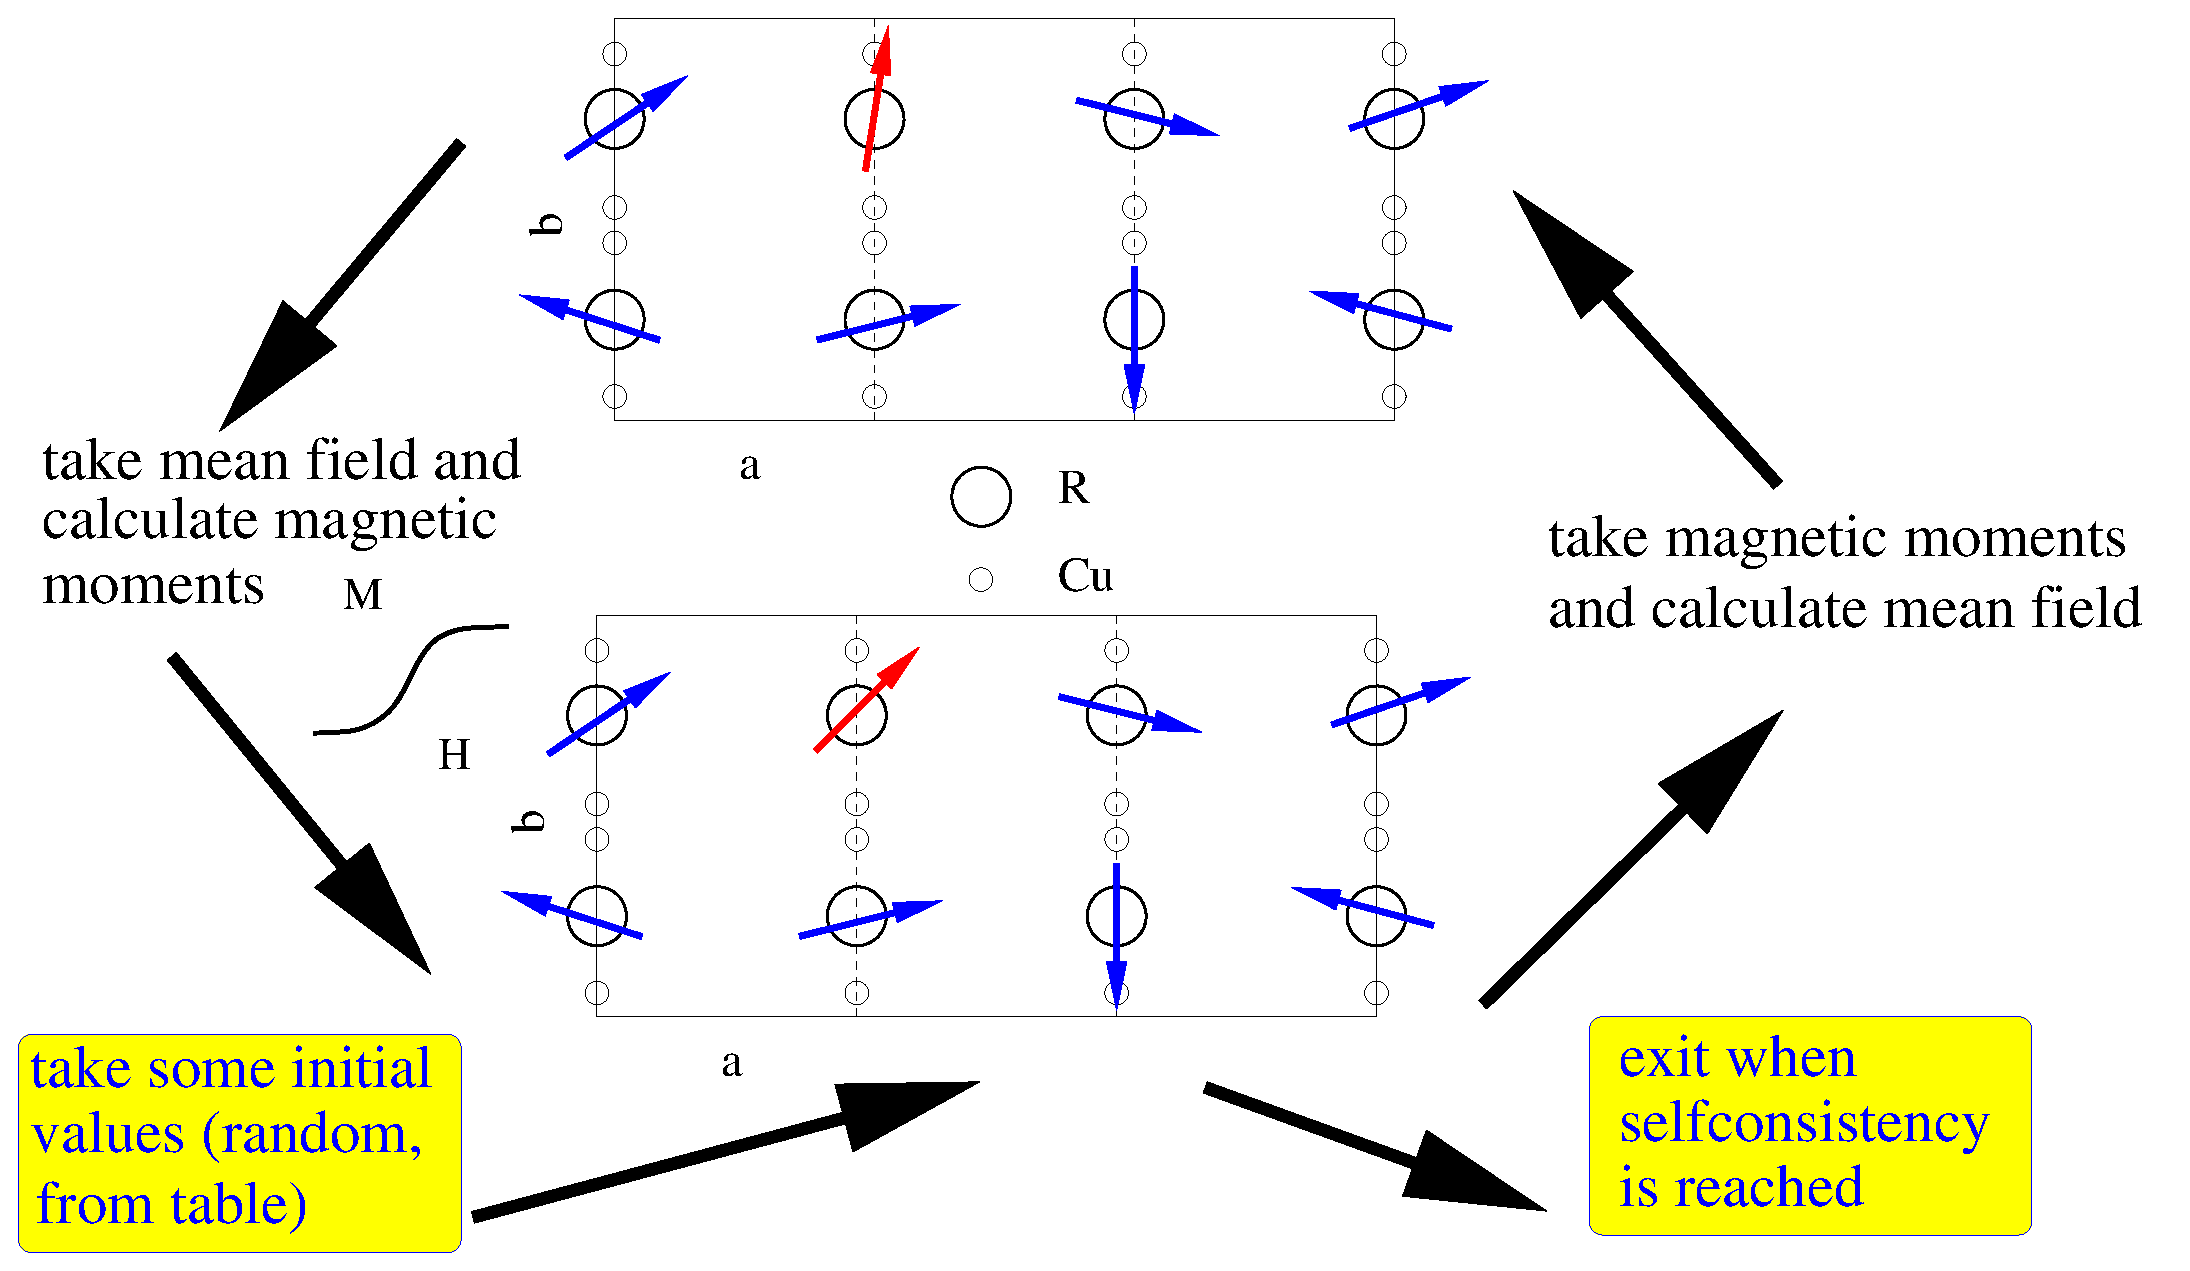
\includegraphics[angle=0,width=0.9\columnwidth]{figsrc/fecalc.eps}
\caption{\label{fecalc}Mean field process of sub {\prg fecalc}.}
\end{figure}

 
\subsubsection{Example {\prg mcphas.ini\index{mcphas.ini}} file for a simple antiferromagnet}

Here is an example of {\prg mcphas.ini\index{mcphas.ini}}, the comments describe the meaning of the different
parameters:

\input{mcphas.ini}



\subsubsection{{\prg mcphas.j\index{mcphas.j}} - lattice and exchange parameters}\label{mcphasj}
This file provides the information about 
the crystallographic
 structure and the magnetic exchange interactions.
For every atom in the crystallographic basis there
has to be given the coordinates, the number of neighbours to be considered, the 
Land\'e factor $g_J$, the single ion property filename and  a set of exchange parameters.
If the exchange parameters (and neighbour positions) are not known for your system, you 
can use the program module {\prg makenn\index{makenn}} (see section \ref{addprog}) to generate 
a list of nearest neighbours and
exchange parameters, currently implemented in {\prg makenn\index{makenn}} are dipolar interactions,
exchange interactions via the Bethe-Slater curve or the RKKY model. Note that in order
to use {\prg makenn\index{makenn}} you have to set up a working {\prg mcphas.j\index{mcphas.j}} file, which may or
may not contain neighbours and interactions.

Use program {\prg addj\index{addj}} to add exchange parameter set stored in different 
such {\prg .j} files (see section~\ref{addprog}).



\begin{description}
\item [Line 1,2:] Comment Lines
\item [Line 3:] lattice constants a,b,c and crystal angles alpha, beta, gamma 
\item [Line 4-6:] primitive lattice vectors
\item [Line 7:] Number of atoms in the primitive crystallographic unit cell ({\prg nofatoms})
\item [Line 8:] a comment line with stars
\item [Line 9:] coordinates  ($d_a$,$d_b$,$d_c$) of 1$^{st}$ magnetic ion in the crystallographic unit cell  with
respect to the lattice vectors $\vec a$,$\vec b$,$\vec c$. The number of neighbours of this 
ion, for which interaction constants are given in the interaction table (nofneighbours). 
If {\prg diagonalexchange}
is set to 0 the 9 components of the exchange tensor are given in column 4-12. 
If {\prg diagonalexchange}
 is 1, only 3 components are given (column 4-6).
If {\prg diagonalexchange}
 is 2, specific components of the exchange tensor can be given in columns 4 onwards. The indices of these components
 must be given in the following line (Line 9a below).
The Land\'e factor of the ion (gJ) and the file name of the corresponding single ion
parameter file (cffilename).
\item [Line 9a:]  If {\prg diagonalexchange=2}, then this line gives the indices of the exchange tensor corresponding to 
 the columns 4 onwards. It must have a variable called {\prg indexexchange} followed by a list of names of components of the interaction
 tensor separated by space. E.g.
 \verb|  #! indexexchange= JaJb JbJc  | 
means column 4 gives the the interaction constant between the
 first angular momentum component of the current ion with the second angular momentum component of its neighbour, whilst 
 column 5 has the interaction constant between the second angular momentum component of this ion with the third component of its
 neighbour. Alternatively, pairs of numbers may be given, as in \verb|  #! indexexchange= 1,2 2,3  |
 Additionally another parameter {\prg symmetricexchange} can be set to 1, where the value in each column is also used 
 for the transposed tensor component. Thus \verb|  #! symmetricexchange=1 indexexchange= JaJb  | is the same as \\
 \verb|  #! indexexchange= JaJb JbJa  | where the 4th and 5th column are the same.
\item [Line 10:]  Comment line
\item [Line 11-(10+nofneighbours):] Interaction table for ion number 1.   
Note: the neighbour coordinates (column 1-3) are given with respect to the lattice vectors
$\vec a$,$\vec b$,$\vec c$. The program then calculates from these values the coordinates
with respect to the primitive lattice $\vec r_1$,~$\vec r_2$,~$\vec r_3$.
($ d_a \vec a + d_b \vec b + d_c \vec c = d_1 \vec r_1 + d_2 \vec r_2 + d_3 \vec r_3$).
Column 4,5,6 \dots contain the components of the interaction tensor $\stackrel{=}{\mathcal J}$. 
Note that in case of non-orthogonal axes the 
components of the moments and the interaction tensor $Ja, Jb, Jc, Jaa, Jbb, Jcc, Jab ...$ 
refer to the orthogonal coordinate system
defined with respect to the nonorthogonal lattice $\vec a,\vec b,\vec c$ as
$Jb||\vec b$, $Jc||(\vec a \times \vec b)$ and $Ja$ perpendicular to $Jb$ and $Jc$.
\item [Line (11+nofneighbours) - end:] for each ion in the unit cell line 8 - (10+nofneighbours)
are repeated.
\end{description}


\vspace{0.5cm}

{\small {\bf Information for experienced users:}
\begin{description}
\item[\prg mcphas.jjj:]
format of exchange parameter file, which only needs a reduced set of exchange
parameters in the input file. Using the program {\prg jjj2j} the file can be transformed
to {\prg mcphas.j\index{mcphas.j}} by adding lines for all the equivalent neighbours. The format definition
of {\prg mcphas.jjj} is the same as {\prg mcphas.j\index{mcphas.j}}, however each line denotes several
equivalent neighbour atoms (instead of only one in {\prg mcphas.j\index{mcphas.j}}) according to the
 following rules:
\begin{itemize}
\item If a nonzero coordinate $d_a$ (or $d_b$,$d_c$) in the interaction table
 corresponds to it's value at the nearest
 lattice point of the primitive lattice,
  additional interactions of the same size
with  neighbours with coordinate $-d_a$ (or $-d_b$,$-d_c$, respectively)
are taken into account. This
holds for each of the three coordinates $d_a$,$d_b$ and $d_c$
 resulting in a maximum
number of 8 equivalent neighbours per line in the interaction table.
\item If the value of $d_a$ (or $d_b$,$d_c$) is zero or differs
from it's value at the nearest lattice point of the primitive lattice, it is 
changed to the value at the nearest lattice point and {\bf no} interaction 
with  neighbours with coordinates $-d_a$ (or $-d_b$,$-d_c$) is
 taken into account. If such
 interaction is needed it may be given in a different line and may
have different magnitude. In this way also crystallographic lattices
with no mirror symmetry may be described.
\end{itemize}
\item[\prg mcphas.coq:]   exchange parameters etc [ in old format]...see examples for details, use {\prg coq2jjj} to 
transform {\prg mcphas.coq} to {\prg mcphas.jjj} format
\end{description}

}


\subsubsection{Example {\prg mcphas.j\index{mcphas.j}} file for a simple antiferromagnet}

Here are example files of a tetragonal antiferromagnet with nearest neighbour interactions, all
files are equivalent:

{\small
\begin{verbatim} 
# simple antiferromagnet 
#<!--mcphase.mcphas.j-->
#***************************************************************
# Lattice Constants (A)
#! a=4.3843 b=4.3843 c=2.4194 alpha=  90 beta=  90 gamma=  90
#! r1a=   1 r2a=   0 r3a=   0
#! r1b=   0 r2b=   1 r3b=   0   primitive lattice vectors [a][b][c]
#! r1c=   0 r2c=   0 r3c=   1
#! nofatoms=1  nofcomponents=3  number of atoms in primitive unit cell/number of components of each spin
# ****************************************************************************
#! da=  0 [a] db=  0 [b] dc=  0 nofneighbours=2 diagonalexchange=0 gJ=0.857143 cffilename=Ce3p.sipf
# da[a] db[b] dc[c] Jaa[meV] Jbb[meV] Jcc[meV] Jab[meV] Jba[meV] Jac[meV] Jca[meV] Jbc[meV] Jcb[meV]
+0	+0	+1	-0.1	-0.1	-0.1   0  0  0  0  0  0
+0	+0	-1	-0.1	-0.1	-0.1   0  0  0  0  0  0
#\end{verbatim}
}

Using diagonalexchange this may be shortened to

{\small
\begin{verbatim} 
# simple antiferromagnet 
#<!--mcphase.mcphas.j-->
#***************************************************************
# Lattice Constants (A)
#! a=4.3843 b=4.3843 c=2.4194 alpha=  90 beta=  90 gamma=  90
#! r1a=   1 r2a=   0 r3a=   0
#! r1b=   0 r2b=   1 r3b=   0   primitive lattice vectors [a][b][c]
#! r1c=   0 r2c=   0 r3c=   1
#! nofatoms=1  nofcomponents=3  number of atoms in primitive unit cell/number of components of each spin
# ****************************************************************************
#! da=  0 [a] db=  0 [b] dc=  0 nofneighbours=2 diagonalexchange=1 gJ=0.857143 cffilename=Ce3p.sipf
# da[a] db[b] dc[c] Jaa[meV] Jbb[meV] Jcc[meV] Jab[meV] Jba[meV] Jac[meV] Jca[meV] Jbc[meV] Jcb[meV]
+0	+0	+1	-0.1	-0.1	-0.1   
+0	+0	-1	-0.1	-0.1	-0.1   
#\end{verbatim}
}

with indexexchange option the sequence of two ion interaction parameters can be changed and
zero parameters may be omitted:

{\small
\begin{verbatim} 
# simple antiferromagnet 
#<!--mcphase.mcphas.j-->
#***************************************************************
# Lattice Constants (A)
#! a=4.3843 b=4.3843 c=2.4194 alpha=  90 beta=  90 gamma=  90
#! r1a=   1 r2a=   0 r3a=   0
#! r1b=   0 r2b=   1 r3b=   0   primitive lattice vectors [a][b][c]
#! r1c=   0 r2c=   0 r3c=   1
#! nofatoms=1  nofcomponents=3  number of atoms in primitive unit cell/number of components of each spin
# ****************************************************************************
#! da=  0 [a] db=  0 [b] dc=  0 nofneighbours=2 diagonalexchange=2 gJ=0.857143 cffilename=Ce3p.sipf
# da[a] db[b] dc[c] Jaa[meV] Jbb[meV] Jcc[meV] Jab[meV] Jba[meV] Jac[meV] Jca[meV] Jbc[meV] Jcb[meV]
#! indexexchange = JaJa JaJc JcJa JbJb JcJc
+0	+0	+1	-0.1 0 0 -0.1	-0.1  
+0	+0	-1	-0.1 0 0 -0.1	-0.1  
#\end{verbatim}
}

{\small
\begin{verbatim} 
# simple antiferromagnet 
#<!--mcphase.mcphas.j-->
#***************************************************************
# Lattice Constants (A)
#! a=4.3843 b=4.3843 c=2.4194 alpha=  90 beta=  90 gamma=  90
#! r1a=   1 r2a=   0 r3a=   0
#! r1b=   0 r2b=   1 r3b=   0   primitive lattice vectors [a][b][c]
#! r1c=   0 r2c=   0 r3c=   1
#! nofatoms=1  nofcomponents=3  number of atoms in primitive unit cell/number of components of each spin
# ****************************************************************************
#! da=  0 [a] db=  0 [b] dc=  0 nofneighbours=2 diagonalexchange=2 gJ=0.857143 cffilename=Ce3p.sipf
# da[a] db[b] dc[c] Jaa[meV] Jbb[meV] Jcc[meV] Jab[meV] Jba[meV] Jac[meV] Jca[meV] Jbc[meV] Jcb[meV]
#! indexexchange = 1,1 1,3, 3,1 2,2 3,3
+0	+0	+1	-0.1 0 0 -0.1	-0.1  
+0	+0	-1	-0.1 0 0 -0.1	-0.1  
#\end{verbatim}
}


using symmetricexchange together with indexexchange will assume that the interaction tensor is symmetic and 
only half of it may be given:

{\small
\begin{verbatim} 
# simple antiferromagnet 
#<!--mcphase.mcphas.j-->
#***************************************************************
# Lattice Constants (A)
#! a=4.3843 b=4.3843 c=2.4194 alpha=  90 beta=  90 gamma=  90
#! r1a=   1 r2a=   0 r3a=   0
#! r1b=   0 r2b=   1 r3b=   0   primitive lattice vectors [a][b][c]
#! r1c=   0 r2c=   0 r3c=   1
#! nofatoms=1  nofcomponents=3  number of atoms in primitive unit cell/number of components of each spin
# ****************************************************************************
#! da=  0 [a] db=  0 [b] dc=  0 nofneighbours=2 diagonalexchange=2 gJ=0.857143 cffilename=Ce3p.sipf
# da[a] db[b] dc[c] Jaa[meV] Jbb[meV] Jcc[meV] Jab[meV] Jba[meV] Jac[meV] Jca[meV] Jbc[meV] Jcb[meV]
#! symmetricexchange=1 indexexchange = JaJa JaJc JbJb JcJc
+0	+0	+1	-0.1 0  -0.1	-0.1  
+0	+0	-1	-0.1 0  -0.1	-0.1  
#\end{verbatim}
}


\subsubsection{Single Ion Property Input Files}\label{sifile}

In order to speed up calculations or treat special problems a large 
variety of single ion modules is available. This includes the
option to load a user written single ion module. Details are 
given in chapter~\ref{simod}.

The first time user of {\prg McPhase} should use the module {\prg so1ion}\index{so1ion} and 
create an appropriate single ion property input file as described in
section \ref{cf1ion}. A good starting point are several examples
given in directory {\prg examples}.


\subsubsection{Example single ion property file  for a simple antiferromagnet}

Here is an example file {\prg mcphas.cf1} describing the anisotropy of a 
simple antiferromagnet with Ce atoms having basal plane anisotropy. Note the
axis convention xyz$||$abc, in case of non-orthogonal axes the convention 
is $y||\vec b$, $z||(\vec a \times \vec b)$ and $x$ perpendicular to $y$ and $z$.


\input{mcphas.cf1}

\subsubsection{{\prg mcphas.tst\index{mcphas.tst}} - input file of test spin-configurations (optional)}
This file is optional and contains
some test momentum configurations to be used for the calculation
             of the free energy. Mind that
\begin{itemize}
\item  in the file header the number of atoms in the primitive
       crystallographic unit cell and the number of components
       of the spin vector have to be given.
\item  at the end of the
 file there must be no empty lines !
\end{itemize}

The momentum - configurations tables always refer to spins sitting on
the primitive lattice ${\mbf r}_i$. If more than one atom is in
the primitive basis, the momentum gets $3n$ components ($n=$ number
of atoms in the crystallographic basis). See {\prg ./examples/ndcu2b\_new/} for
examples of a two atom basis. Units of these tables are that of total 
angular momentum $<J>$.

\subsubsection{Example {\prg mcphas.tst\index{mcphas.tst}} file  for a simple antiferromagnet}

Here is the file {\prg mcphas.tst\index{mcphas.tst}} for the simple antiferromagnet example
describing some spin configurations
to be used as starting values for the mean field process:

\input{mcphas.tst}
Note, in case of non-orthogonal axes the convention 
is $mb||\vec b$, $mc||(\vec a \times \vec b)$ and $ma$ perpendicular to $mb$ and $mc$.

\subsubsection{subdirectory {\prg ./results} - directory where calculated data is stored}

In order to be able to save the results of a calculation the directory {\prg ./results} has to
exist. Mind that all files in this directory will be overwritten without warning. 

\subsubsection{subdirectory {\prg ./fit} - experimental data for fit (optional) } 

In order that {\prg McPhase} can calculate the standard deviation between
 experimental data and the results of the simulation, some experimental data
 can be given in the subdirectory {\prg ./fit}. The filenames and the data-format
 are the same as the output files of {\prg McPhas}, e.g. {\prg mcphas.fum}, {\prg mcphas.hkl}
 etc. {\prg McPhase} looks into the directory {\prg ./fit} and if it finds any
 of these files, the standard deviation is increased correspondingly. 

What measurement data can be used to calculate a standard deviation ?

\begin{description}
\item[{\prg mcphas.fum}] if given in column 11, 12, 13 in {\prg ./fit/mcphas.fum} the
            magnetisation in the $a$, $b$ and $c$ direction is used for calculation
	    of the standard deviation sta. The standard deviation is calculated
	    as ${\rm sta}=\sum_{\rm data points i} ({\mbf m}_i^{calc}-{\mbf m}_i^{meas})^2$.
	    All three components of the magnetic moment have to be given and are used.

\end{description}

Note that the measured data has to be given in those (H-T) points which are 
calculated by mcphas\index{mcphas} in order to be used by the program to increase {\prg sta}.
It is usually most effective to fit only few data points, because a large set
of data points will not improve the quality of the fit and only require a large
amount of calculation time.



\subsection{Starting a simulation}
\label{start}

To start the simulation goto the directory containing the
input files {\prg mcphas.ini, mcphas.j, etc. } and type

\begin{description}
\item[\prg mcphas] to run the program generating stepwise $H-T$ values 
              in a loop given by {\prg mcphas.ini\index{mcphas.ini}} (you can also press the
              symbol in the {\prg McPhase - Explorer} window).
\item[\prg mcphas\index{mcphas} [file]]  to run the program with an input file --   
             {\prg file} contains T ha hb hc values to be calculated 
             if [file] is not given, xmin xmax xstep (xT xHa xHb xHc)
             ymin ymax ystep (yT yHa yHb yHc) is read from file {\prg mcphas.ini\index{mcphas.ini}}
	     and phase diagram is calculated
\item[\prg mcphas\index{mcphas} -h]  to  print help and version of {\prg McPhas}.
\item[\prg mcphas\index{mcphas} -stamax 14]  end mcphas\index{mcphas} if standard deviation exceeds 14.
\item[\prg mcphas\index{mcphas} -a] avoid overwriting output files in results, append new results to existing files
\item[\prg mcphas\index{mcphas} -v]  to  enable verbose mode with lots of messages of {\prg McPhas}. Specifically
the verbose mode enables the following features:
  \begin{itemize}
			          \item more information is printed out, 
			          \item the q-vectors file {\prg ./results/mcphas.qvc} will contain 
				    the explicit spin configurations
			          \item the display\index{display} on screen (ghostview window using 
				     {\prg ./results/.sps.eps}) will be updated not only 
				    when a H-T point has been finished but always 
				    when a structure with smaller free energy 
				    has been stabilised
  \end{itemize}
\item[\prg mcphasit\index{mcphas}] to start mcphase in commandline mode without opening any window
\end{description}

\vspace{1cm}
{\em Exercises:}
\begin{itemize}
\item Look at the input files for {\prg McPhase} given in the directory
{\prg examples/ndcu2b\_new}.  How many atoms are contained in the crystallographic basis ?
\item
Start the simulation by typing the command {\prg mcphas}.
\end{itemize}



\subsection{Options for a running simulation}
... when the program is running, the options in the main window
can be changed. Pressing ''displayall'' displays the current spin-configuration
at each iteration step. Pressing ''log fe vs Q'' appends free energy vs Q
data to {\prg mcphas.log} for every ($T-H$) point.


The file {\prg ./results/.spins.eps} is used to show the information about the currently calculated
spin structure on the screen using the postscript file viewer ghostview.

The file {\prg ./results/.mcphas.fum} contains the information of the magnetisation curve
which is currently calculated. This information is automatically displayed on the screen.


The program {\prg display} (see section \ref{display}) can be used 
for the online display\index{display} of any other
curve(s).


\subsection{Output Files - {\prg mcphas.qvc,phs,sps,mf,fum,j1...,xyt,hkl} }\label{outputfiles}
 (in directory ./results/ after a simulation run) 

\begin{figure}[htb]%h=here, t=top, b=bottom, p=separate figure page
\begin{center}\leavevmode
\includegraphics[angle=0, width=0.3\textwidth]{figsrc/magnetization_ndcu2.ps}
\end{center}
\caption{Calculated magnetisation of NdCu$_2$ for field parallel to the orthorhombic $b$-direction.}
\label{magnetization}
\end{figure}

\begin{figure}[htb]%h=here, t=top, b=bottom, p=separate figure page
\begin{center}\leavevmode
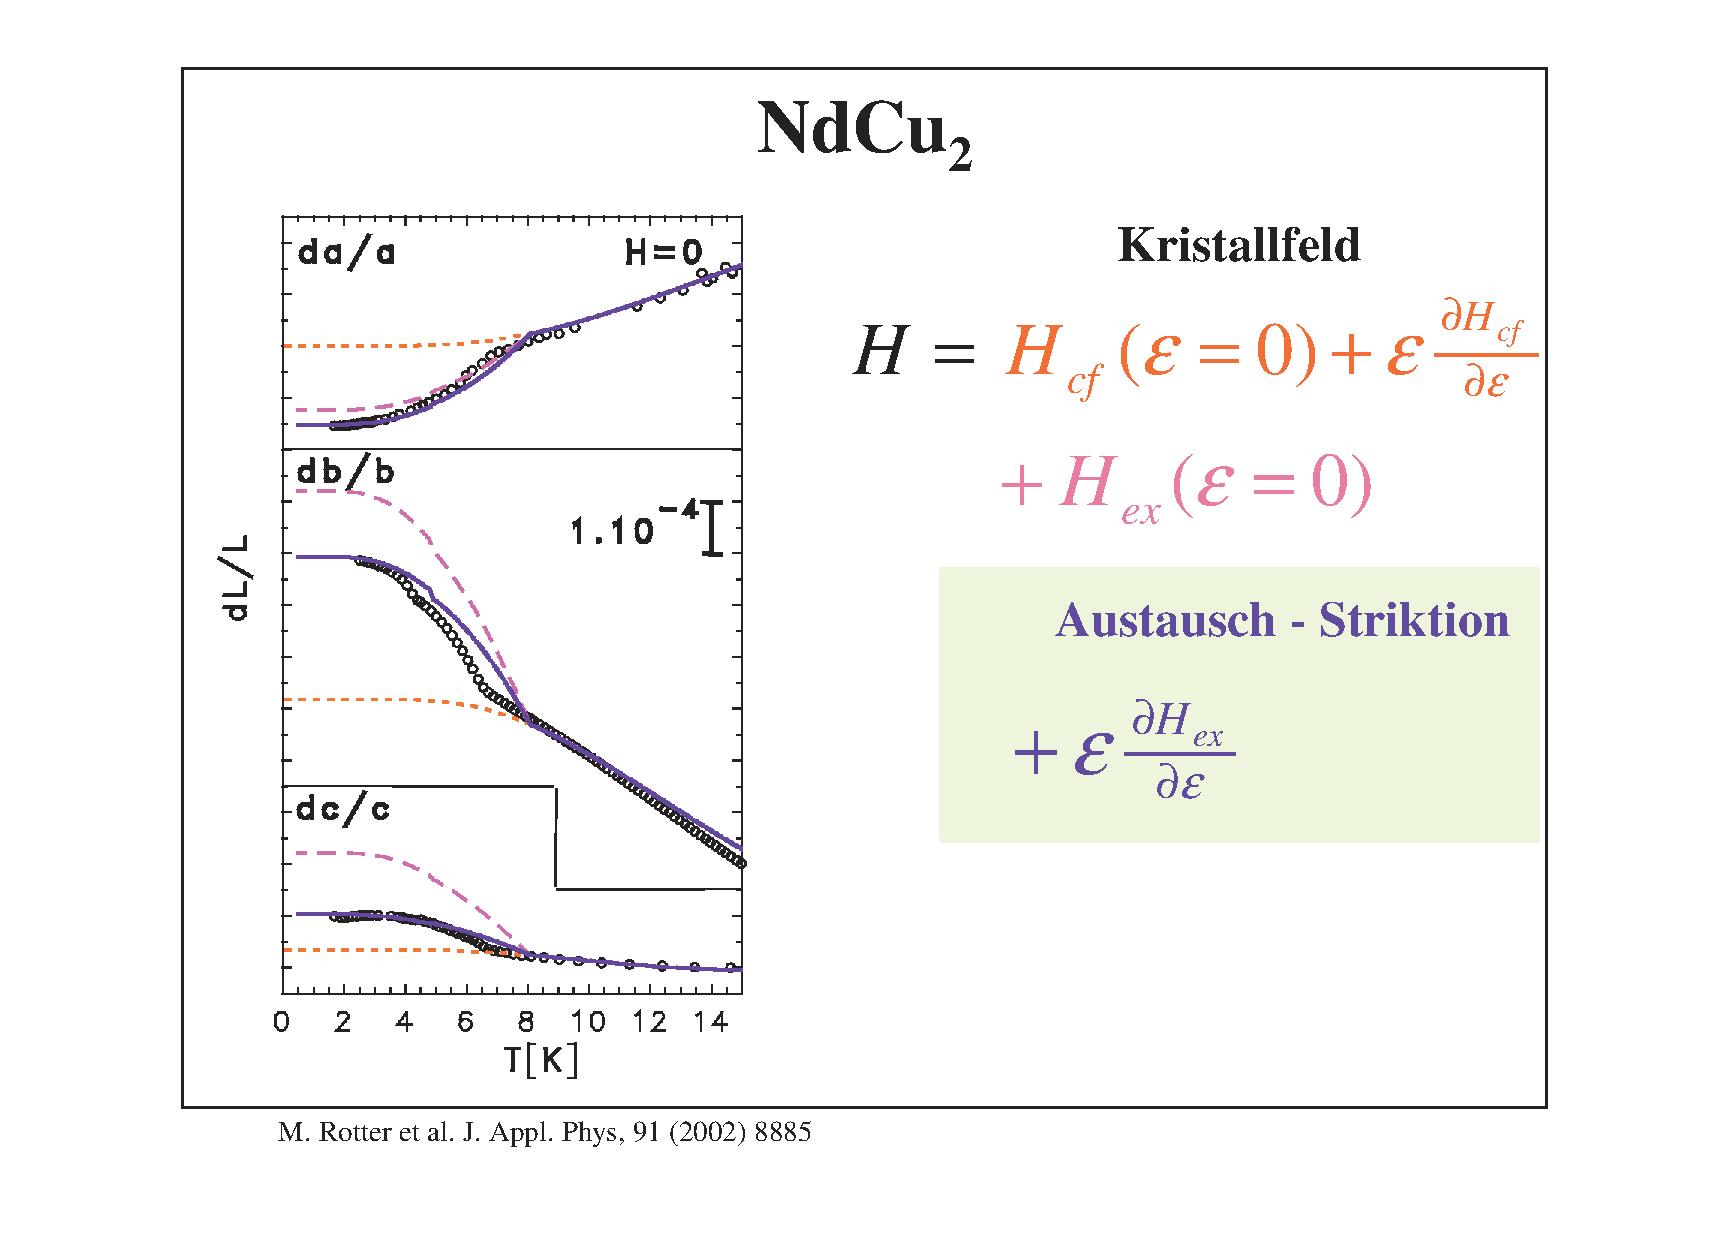
\includegraphics[angle=0, width=0.8\textwidth]{figsrc/magnetostriction_ndcu2.eps}
\end{center}
\caption{Calculated spontaneous magnetostriction of NdCu$_2$.}
\label{magnetostrictiongraphic}
\end{figure}

\begin{description}
\item [\prg mcphas.qvc]    the set of test q-vectors used for calculation of free energy.
                           Components of these q vectors refer to the reciprocal lattice $\vec a^*,\vec b^*,\vec c^*$.
\item [\prg mcphas.phs]    spin-configuration table of different types of spin-configurations. 
                            Note, in case of non-orthogonal axes the convention in these tables 
                            is $mb||\vec b$, $mc||(\vec a \times \vec b)$ and $ma$ perpendicular to $mb$ and $mc$.

                           {\em Note}: 
                           there is no natural criteria for deciding, if one spin-configuration is
			   different from another one. Therefore the list of ''different''
			   spin-configurations is dependent on the meaning of ''different''.
			   
			   The program {\prg McPhase} decides whether a spin-configuration is
			   different from another by a simple criteria, namely by the
			   angle between the spins. Comparing two spin configurations it calculates
			   the angle between corresponding spins and if for one spin the
			   angle is not small, the configuration is treated as a different
			   configuration. Therefore for example a ferromagnet with moments
			   in $a$ has a different spin configuration than a ferromagnet with
			   moments in $b$ direction. 
\item [\prg mcphas.sps]    $T-H$ dependence of spin-configuration. The spin configurations stored in this
                           file may be displayed using the program {\prg spins\index{spins}}, an example is given
			   in figure~\ref{spingraphic}.
                            Note, in case of non-orthogonal axes the convention for applied field $Ha, Hb,Hc$ and
                            also for the moment components $ma, mb, mc$ in these tables 
                            is $mb||\vec b$, $mc||(\vec a \times \vec b)$ and $ma$ perpendicular to $mb$ and $mc$.

\item [\prg mcphas.mf]     $T-H$ dependence of exchange field configuration, stored as $g_J \mu_B H_{xc}(i)$(unit is in meV)
                            for i=1,2,...,number of spins in magnetic unit cell.
                            Note, in case of non-orthogonal axes the convention for applied field $Ha, Hb,Hc$ and
                            also for the mean field components in these tables 
                            is $Hb||\vec b$, $Hc||(\vec a \times \vec b)$ and $Ha$ perpendicular to $Hb$ and $Hc$.
\item [\prg mcphas.fum]    free energy, magnetic energy (the derivative with respect to temperature gives the specific %%@
heat),
                           magnetisation data and (if cfield is used with higher order interactions)
                           expectation values of the Stevens Operators $<O_l^m>$ . As an example for the information
			   contained in this file the calculated magnetisation and magnetostriction of NdCu$_2$ is shown in
			   figures~\ref{magnetization} and ~\ref{magnetizationgraphic}.
                            Note, in case of non-orthogonal axes the convention for applied field $Ha, Hb,Hc$ and
                            also for the magnetisation components $ma,mb,mc$ in these tables 
                            is $Hb||\vec b$, $Hc||(\vec a \times \vec b)$ and $Ha$ perpendicular to $Hb$ and $Hc$.

\item [\prg mcphas1.j1 .j1 .j2 ...] 
               spin-spin correlation functions for sub-lattice 1 neighbour 1 2 ...
	       (linear combination is proportional to magnetostriction)
	       The spin-spin correlation functions for neighbour $k$ are defined by
	       the following sum of dyadic products:

	       \begin{equation}
	        \frac{1}{n}\sum_{s=1}^n <{\mbf J}^s> \times  <{\mbf J}^{s+k}>
	       \end{equation}
	       with $n$ being the number of moments in the magnetic unit cell.
	       Single ion and two-ion magnetostriction can be calculated using the $<O_l^m>$ and the
	       spin-spin correlation functions. As an example the magnetostriction analysis of
	       NdCu$_2$ is shown in figure~\ref{magnetostrictiongraphic}. For details 
             please refer to~\cite{rotter02-8885}.
                            Note, in case of non-orthogonal axes the convention for applied field $Ha, Hb,Hc$ and
                            also for the moment components in these tables 
                            is $Hb||\vec b$, $Hc||(\vec a \times \vec b)$ and $Ha$ perpendicular to $Hb$ and $Hc$.
\item [\prg mcphas.xyt]    phase diagram as x,y,T, H, phase-number j according to spin-configuration table
               given in mcphas.phs, a periodicity key, nettomoments <J>.
 Figure~\ref{phasediagramgraphic}
	       shows the phase diagram of NdCu$_2$ for magnetic fields parallel to the orthorhombic $b$-direction.
                            Note, in case of non-orthogonal axes the convention for applied field $Ha, Hb,Hc$ 
                             in these tables 
                            is $Hb||\vec b$, $Hc||(\vec a \times \vec b)$ and $Ha$ perpendicular to $Hb$ and $Hc$.
\item [\prg mcphas.hkl]    calculated (unpolarised) neutron diffraction data (the calculated magnetic intensities
    correspond to the magnetic structure + Polarisation factor. The
    Lorentz-factor , magnetic form factor and  instrumental corrections are not calculated.)
 As an example figure~\ref{neutintgraphic}
    shows the calculated temperature dependence of magnetic amplitudes for NdCu$_2$.
                           $h,k,l$ refer to the reciprocal lattice $\vec a^*,\vec b^*,\vec c^*$.
                            Note, in case of non-orthogonal axes the convention for applied field $Ha, Hb,Hc$ 
                             in these tables 
                            is $Hb||\vec b$, $Hc||(\vec a \times \vec b)$ and $Ha$ perpendicular to $Hb$ and $Hc$.
    
\item [\prg mcphasa.hkl]    Fourier Transform of the $a$-component of the magnetic Moments.
                           $h,k,l$ refer to the reciprocal lattice $\vec a^*,\vec b^*,\vec c^*$.
                            Note, in case of non-orthogonal axes the convention for applied field $Ha, Hb,Hc$ and
                            the magnetic moment component in these tables 
                            is $Hb||\vec b$, $Hc||(\vec a \times \vec b)$ and $Ha$ perpendicular to $Hb$ and $Hc$.
\item [\prg mcphasb.hkl]    Fourier Transform of the $b$-component of the magnetic Moments.
                           $h,k,l$ refer to the reciprocal lattice $\vec a^*,\vec b^*,\vec c^*$.
                            Note, in case of non-orthogonal axes the convention for applied field $Ha, Hb,Hc$ and
                            the magnetic moment component in these tables 
                            is $Hb||\vec b$, $Hc||(\vec a \times \vec b)$ and $Ha$ perpendicular to $Hb$ and $Hc$.
\item [\prg mcphasc.hkl]    Fourier Transform of the $c$-component of the magnetic Moments.
                           $h,k,l$ refer to the reciprocal lattice $\vec a^*,\vec b^*,\vec c^*$.
                            Note, in case of non-orthogonal axes the convention for applied field $Ha, Hb,Hc$ and
                            the magnetic moment component in these tables 
                            is $Hb||\vec b$, $Hc||(\vec a \times \vec b)$ and $Ha$ perpendicular to $Hb$ and $Hc$.
\end{description} 

\vspace{1cm}
{\em Exercises:}
\begin{itemize}
\item Look at the output files of {\prg McPhase}  in the directory
{\prg examples/ndcu2b\_new/results}.  At which magnetic field
the ferromagnetically aligned state is achieved (at $T=$2~K)?
\item
What is the propagation vector in the different antiferromagnetic phases at $T=$2~K ?
\end{itemize}


Note, in case of non-orthogonal axes the convention 
is $mb||\vec b$, $mc||(\vec a \times \vec b)$ and $ma$ perpendicular to $mb$ and $mc$.

\subsubsection{subdirectory {\prg ./results} - directory where calculated data is stored}

In order to be able to save the results of a calculation the directory {\prg ./results} has to
exist. Mind that all files in this directory will be overwritten without warning. 

\subsubsection{subdirectory {\prg ./fit} - experimental data for fit (optional) } 

In order that {\prg McPhase} can calculate the standard deviation between
 experimental data and the results of the simulation, some experimental data
 can be given in the subdirectory {\prg ./fit}. The filenames and the data-format
 are the same as the output files of {\prg McPhas}, e.g. {\prg mcphas.fum}, {\prg mcphas.hkl}
 etc. {\prg McPhase} looks into the directory {\prg ./fit} and if it finds any
 of these files, the standard deviation is increased correspondingly. 

What measurement data can be used to calculate a standard deviation ?

\begin{description}
\item[{\prg mcphas.fum}] if given in column 11, 12, 13 in {\prg ./fit/mcphas.fum} the
            magnetisation in the $a$, $b$ and $c$ direction is used for calculation
	    of the standard deviation sta. The standard deviation is calculated
	    as ${\rm sta}=\sum_{\rm data points i} ({\mbf m}_i^{calc}-{\mbf m}_i^{meas})^2$.
	    All three components of the magnetic moment have to be given and are used.

\end{description}

Note that the measured data has to be given in those (H-T) points which are 
calculated by mcphas\index{mcphas} in order to be used by the program to increase {\prg sta}.
It is usually most effective to fit only few data points, because a large set
of data points will not improve the quality of the fit and only require a large
amount of calculation time.



\subsection{Starting a simulation}
\label{start}

To start the simulation goto the directory containing the
input files {\prg mcphas.ini, mcphas.j, etc. } and type

\begin{description}
\item[\prg mcphas] to run the program generating stepwise $H-T$ values 
              in a loop given by {\prg mcphas.ini\index{mcphas.ini}} (you can also press the
              symbol in the {\prg McPhase - Explorer} window).
\item[\prg mcphas\index{mcphas} [file]]  to run the program with an input file --   
             {\prg file} contains T ha hb hc values to be calculated 
             if [file] is not given, xmin xmax xstep (xT xHa xHb xHc)
             ymin ymax ystep (yT yHa yHb yHc) is read from file {\prg mcphas.ini\index{mcphas.ini}}
	     and phase diagram is calculated
\item[\prg mcphas\index{mcphas} -h]  to  print help and version of {\prg McPhas}.
\item[\prg mcphas\index{mcphas} -stamax 14]  end mcphas\index{mcphas} if standard deviation exceeds 14.
\item[\prg mcphas\index{mcphas} -a] avoid overwriting output files in results, append new results to existing files
\item[\prg mcphas\index{mcphas} -v]  to  enable verbose mode with lots of messages of {\prg McPhas}. Specifically
the verbose mode enables the following features:
  \begin{itemize}
			          \item more information is printed out, 
			          \item the q-vectors file {\prg ./results/mcphas.qvc} will contain 
				    the explicit spin configurations
			          \item the display\index{display} on screen (ghostview window using 
				     {\prg ./results/.sps.eps}) will be updated not only 
				    when a H-T point has been finished but always 
				    when a structure with smaller free energy 
				    has been stabilised
  \end{itemize}
\item[\prg mcphasit\index{mcphas}] to start mcphase in commandline mode without opening any window
\end{description}

\vspace{1cm}
{\em Exercises:}
\begin{itemize}
\item Look at the input files for {\prg McPhase} given in the directory
{\prg examples/ndcu2b\_new}.  How many atoms are contained in the crystallographic basis ?
\item
Start the simulation by typing the command {\prg mcphas}.
\end{itemize}



\subsection{Options for a running simulation}
... when the program is running, the options in the main window
can be changed. Pressing ''displayall'' displays the current spin-configuration
at each iteration step. Pressing ''log fe vs Q'' appends free energy vs Q
data to {\prg mcphas.log} for every ($T-H$) point.


The file {\prg ./results/.spins.eps} is used to show the information about the currently calculated
spin structure on the screen using the postscript file viewer ghostview.

The file {\prg ./results/.mcphas.fum} contains the information of the magnetisation curve
which is currently calculated. This information is automatically displayed on the screen.


The program {\prg display} (see section \ref{display}) can be used 
for the online display\index{display} of any other
curve(s).


\subsection{Output Files - {\prg mcphas.qvc,phs,sps,mf,fum,j1...,xyt,hkl} }\label{outputfiles}
 (in directory ./results/ after a simulation run) 

\begin{figure}[htb]%h=here, t=top, b=bottom, p=separate figure page
\begin{center}\leavevmode
\includegraphics[angle=0, width=0.3\textwidth]{figsrc/magnetization_ndcu2.ps}
\end{center}
\caption{Calculated magnetisation of NdCu$_2$ for field parallel to the orthorhombic $b$-direction.}
\label{magnetization}
\end{figure}

\begin{figure}[htb]%h=here, t=top, b=bottom, p=separate figure page
\begin{center}\leavevmode
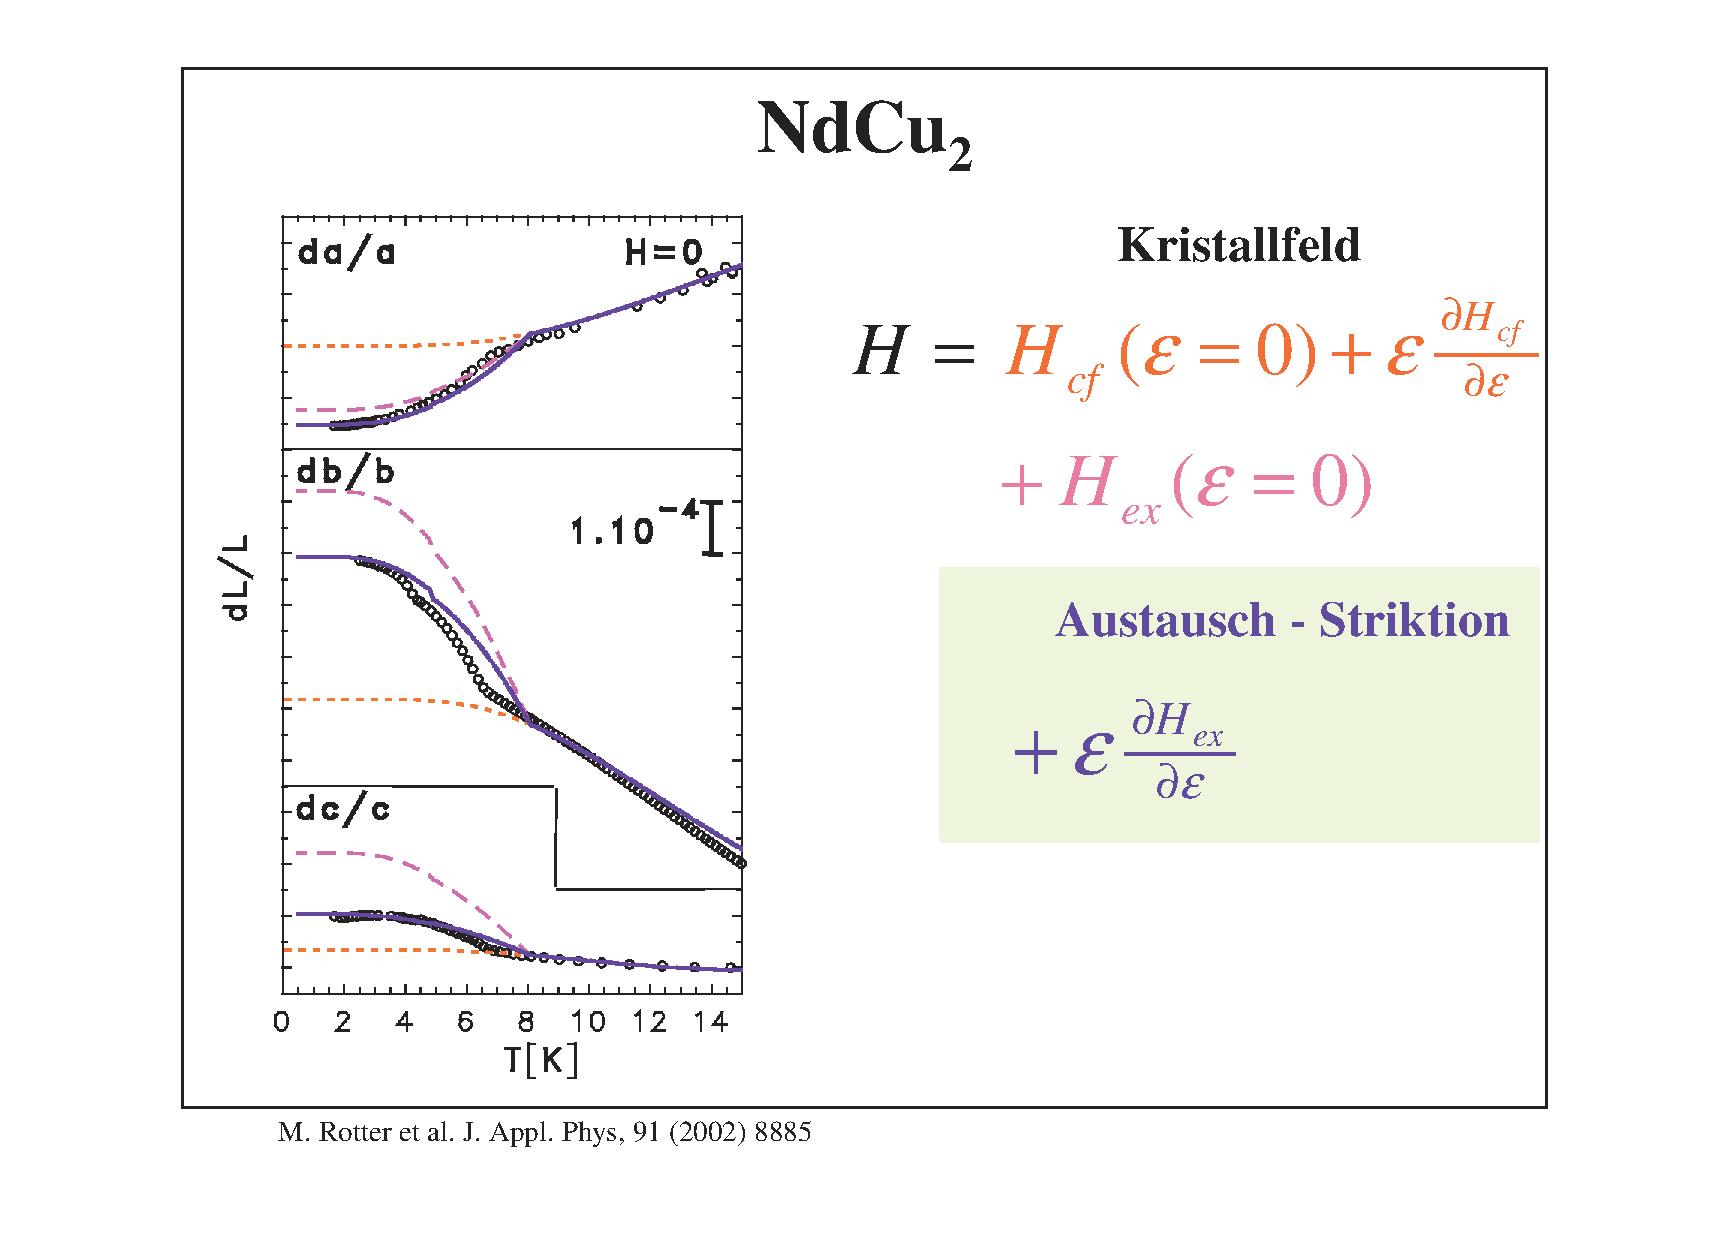
\includegraphics[angle=0, width=0.8\textwidth]{figsrc/magnetostriction_ndcu2.eps}
\end{center}
\caption{Calculated spontaneous magnetostriction of NdCu$_2$.}
\label{magnetostrictiongraphic}
\end{figure}

\begin{description}
\item [\prg mcphas.qvc]    the set of test q-vectors used for calculation of free energy.
                           Components of these q vectors refer to the reciprocal lattice $\vec a^*,\vec b^*,\vec c^*$.
\item [\prg mcphas.phs]    spin-configuration table of different types of spin-configurations. 
                            Note, in case of non-orthogonal axes the convention in these tables 
                            is $mb||\vec b$, $mc||(\vec a \times \vec b)$ and $ma$ perpendicular to $mb$ and $mc$.

                           {\em Note}: 
                           there is no natural criteria for deciding, if one spin-configuration is
			   different from another one. Therefore the list of ''different''
			   spin-configurations is dependent on the meaning of ''different''.
			   
			   The program {\prg McPhase} decides whether a spin-configuration is
			   different from another by a simple criteria, namely by the
			   angle between the spins. Comparing two spin configurations it calculates
			   the angle between corresponding spins and if for one spin the
			   angle is not small, the configuration is treated as a different
			   configuration. Therefore for example a ferromagnet with moments
			   in $a$ has a different spin configuration than a ferromagnet with
			   moments in $b$ direction. 
\item [\prg mcphas.sps]    $T-H$ dependence of spin-configuration. The spin configurations stored in this
                           file may be displayed using the program {\prg spins\index{spins}}, an example is given
			   in figure~\ref{spingraphic}.
                            Note, in case of non-orthogonal axes the convention for applied field $Ha, Hb,Hc$ and
                            also for the moment components $ma, mb, mc$ in these tables 
                            is $mb||\vec b$, $mc||(\vec a \times \vec b)$ and $ma$ perpendicular to $mb$ and $mc$.

\item [\prg mcphas.mf]     $T-H$ dependence of exchange field configuration, stored as $g_J \mu_B H_{xc}(i)$(unit is in meV)
                            for i=1,2,...,number of spins in magnetic unit cell.
                            Note, in case of non-orthogonal axes the convention for applied field $Ha, Hb,Hc$ and
                            also for the mean field components in these tables 
                            is $Hb||\vec b$, $Hc||(\vec a \times \vec b)$ and $Ha$ perpendicular to $Hb$ and $Hc$.
\item [\prg mcphas.fum]    free energy, magnetic energy (the derivative with respect to temperature gives the specific %%@
heat),
                           magnetisation data and (if cfield is used with higher order interactions)
                           expectation values of the Stevens Operators $<O_l^m>$ . As an example for the information
			   contained in this file the calculated magnetisation and magnetostriction of NdCu$_2$ is shown in
			   figures~\ref{magnetization} and ~\ref{magnetizationgraphic}.
                            Note, in case of non-orthogonal axes the convention for applied field $Ha, Hb,Hc$ and
                            also for the magnetisation components $ma,mb,mc$ in these tables 
                            is $Hb||\vec b$, $Hc||(\vec a \times \vec b)$ and $Ha$ perpendicular to $Hb$ and $Hc$.

\item [\prg mcphas1.j1 .j1 .j2 ...] 
               spin-spin correlation functions for sub-lattice 1 neighbour 1 2 ...
	       (linear combination is proportional to magnetostriction)
	       The spin-spin correlation functions for neighbour $k$ are defined by
	       the following sum of dyadic products:

	       \begin{equation}
	        \frac{1}{n}\sum_{s=1}^n <{\mbf J}^s> \times  <{\mbf J}^{s+k}>
	       \end{equation}
	       with $n$ being the number of moments in the magnetic unit cell.
	       Single ion and two-ion magnetostriction can be calculated using the $<O_l^m>$ and the
	       spin-spin correlation functions. As an example the magnetostriction analysis of
	       NdCu$_2$ is shown in figure~\ref{magnetostrictiongraphic}. For details 
             please refer to~\cite{rotter02-8885}.
                            Note, in case of non-orthogonal axes the convention for applied field $Ha, Hb,Hc$ and
                            also for the moment components in these tables 
                            is $Hb||\vec b$, $Hc||(\vec a \times \vec b)$ and $Ha$ perpendicular to $Hb$ and $Hc$.
\item [\prg mcphas.xyt]    phase diagram as x,y,T, H, phase-number j according to spin-configuration table
               given in mcphas.phs, a periodicity key, nettomoments <J>.
 Figure~\ref{phasediagramgraphic}
	       shows the phase diagram of NdCu$_2$ for magnetic fields parallel to the orthorhombic $b$-direction.
                            Note, in case of non-orthogonal axes the convention for applied field $Ha, Hb,Hc$ 
                             in these tables 
                            is $Hb||\vec b$, $Hc||(\vec a \times \vec b)$ and $Ha$ perpendicular to $Hb$ and $Hc$.
\item [\prg mcphas.hkl]    calculated (unpolarised) neutron diffraction data (the calculated magnetic intensities
    correspond to the magnetic structure + Polarisation factor. The
    Lorentz-factor , magnetic form factor and  instrumental corrections are not calculated.)
 As an example figure~\ref{neutintgraphic}
    shows the calculated temperature dependence of magnetic amplitudes for NdCu$_2$.
                           $h,k,l$ refer to the reciprocal lattice $\vec a^*,\vec b^*,\vec c^*$.
                            Note, in case of non-orthogonal axes the convention for applied field $Ha, Hb,Hc$ 
                             in these tables 
                            is $Hb||\vec b$, $Hc||(\vec a \times \vec b)$ and $Ha$ perpendicular to $Hb$ and $Hc$.
    
\item [\prg mcphasa.hkl]    Fourier Transform of the $a$-component of the magnetic Moments.
                           $h,k,l$ refer to the reciprocal lattice $\vec a^*,\vec b^*,\vec c^*$.
                            Note, in case of non-orthogonal axes the convention for applied field $Ha, Hb,Hc$ and
                            the magnetic moment component in these tables 
                            is $Hb||\vec b$, $Hc||(\vec a \times \vec b)$ and $Ha$ perpendicular to $Hb$ and $Hc$.
\item [\prg mcphasb.hkl]    Fourier Transform of the $b$-component of the magnetic Moments.
                           $h,k,l$ refer to the reciprocal lattice $\vec a^*,\vec b^*,\vec c^*$.
                            Note, in case of non-orthogonal axes the convention for applied field $Ha, Hb,Hc$ and
                            the magnetic moment component in these tables 
                            is $Hb||\vec b$, $Hc||(\vec a \times \vec b)$ and $Ha$ perpendicular to $Hb$ and $Hc$.
\item [\prg mcphasc.hkl]    Fourier Transform of the $c$-component of the magnetic Moments.
                           $h,k,l$ refer to the reciprocal lattice $\vec a^*,\vec b^*,\vec c^*$.
                            Note, in case of non-orthogonal axes the convention for applied field $Ha, Hb,Hc$ and
                            the magnetic moment component in these tables 
                            is $Hb||\vec b$, $Hc||(\vec a \times \vec b)$ and $Ha$ perpendicular to $Hb$ and $Hc$.
\end{description} 

\vspace{1cm}
{\em Exercises:}
\begin{itemize}
\item Look at the output files of {\prg McPhase}  in the directory
{\prg examples/ndcu2b\_new/results}.  At which magnetic field
the ferromagnetically aligned state is achieved (at $T=$2~K)?
\item
What is the propagation vector in the different antiferromagnetic phases at $T=$2~K ?
\end{itemize}





\subsubsection{{\prg mcphas.j\index{mcphas.j}} - lattice and exchange parameters}\label{mcphasj}
This file provides the information about 
the crystallographic
 structure and the magnetic exchange interactions.
For every atom in the crystallographic basis there
has to be given the coordinates, the number of neighbours to be considered, the 
Land\'e factor $g_J$, the single ion property filename and  a set of exchange parameters.
If the exchange parameters (and neighbour positions) are not known for your system, you 
can use the program module {\prg makenn\index{makenn}} (see section \ref{addprog}) to generate 
a list of nearest neighbours and
exchange parameters, currently implemented in {\prg makenn\index{makenn}} are dipolar interactions,
exchange interactions via the Bethe-Slater curve or the RKKY model. Note that in order
to use {\prg makenn\index{makenn}} you have to set up a working {\prg mcphas.j\index{mcphas.j}} file, which may or
may not contain neighbours and interactions.

Use program {\prg addj\index{addj}} to add exchange parameter set stored in different 
such {\prg .j} files (see section~\ref{addprog}).



\begin{description}
\item [Line 1,2:] Comment Lines
\item [Line 3:] lattice constants a,b,c and crystal angles alpha, beta, gamma 
\item [Line 4-6:] primitive lattice vectors
\item [Line 7:] Number of atoms in the primitive crystallographic unit cell ({\prg nofatoms})
\item [Line 8:] a comment line with stars
\item [Line 9:] coordinates  ($d_a$,$d_b$,$d_c$) of 1$^{st}$ magnetic ion in the crystallographic unit cell  with
respect to the lattice vectors $\vec a$,$\vec b$,$\vec c$. The number of neighbours of this 
ion, for which interaction constants are given in the interaction table (nofneighbours). 
If {\prg diagonalexchange}
is set to 0 the 9 components of the exchange tensor are given in column 4-12. 
If {\prg diagonalexchange}
 is 1, only 3 components are given (column 4-6).
If {\prg diagonalexchange}
 is 2, specific components of the exchange tensor can be given in columns 4 onwards. The indices of these components
 must be given in the following line (Line 9a below).
The Land\'e factor of the ion (gJ) and the file name of the corresponding single ion
parameter file (cffilename).
\item [Line 9a:]  If {\prg diagonalexchange=2}, then this line gives the indices of the exchange tensor corresponding to 
 the columns 4 onwards. It must have a variable called {\prg indexexchange} followed by a list of names of components of the interaction
 tensor separated by space. E.g.
 \verb|  #! indexexchange= JaJb JbJc  | 
means column 4 gives the the interaction constant between the
 first angular momentum component of the current ion with the second angular momentum component of its neighbour, whilst 
 column 5 has the interaction constant between the second angular momentum component of this ion with the third component of its
 neighbour. Alternatively, pairs of numbers may be given, as in \verb|  #! indexexchange= 1,2 2,3  |
 Additionally another parameter {\prg symmetricexchange} can be set to 1, where the value in each column is also used 
 for the transposed tensor component. Thus \verb|  #! symmetricexchange=1 indexexchange= JaJb  | is the same as \\
 \verb|  #! indexexchange= JaJb JbJa  | where the 4th and 5th column are the same.
\item [Line 10:]  Comment line
\item [Line 11-(10+nofneighbours):] Interaction table for ion number 1.   
Note: the neighbour coordinates (column 1-3) are given with respect to the lattice vectors
$\vec a$,$\vec b$,$\vec c$. The program then calculates from these values the coordinates
with respect to the primitive lattice $\vec r_1$,~$\vec r_2$,~$\vec r_3$.
($ d_a \vec a + d_b \vec b + d_c \vec c = d_1 \vec r_1 + d_2 \vec r_2 + d_3 \vec r_3$).
Column 4,5,6 \dots contain the components of the interaction tensor $\stackrel{=}{\mathcal J}$. 
Note that in case of non-orthogonal axes the 
components of the moments and the interaction tensor $Ja, Jb, Jc, Jaa, Jbb, Jcc, Jab ...$ 
refer to the orthogonal coordinate system
defined with respect to the nonorthogonal lattice $\vec a,\vec b,\vec c$ as
$Jb||\vec b$, $Jc||(\vec a \times \vec b)$ and $Ja$ perpendicular to $Jb$ and $Jc$.
\item [Line (11+nofneighbours) - end:] for each ion in the unit cell line 8 - (10+nofneighbours)
are repeated.
\end{description}


\vspace{0.5cm}

{\small {\bf Information for experienced users:}
\begin{description}
\item[\prg mcphas.jjj:]
format of exchange parameter file, which only needs a reduced set of exchange
parameters in the input file. Using the program {\prg jjj2j} the file can be transformed
to {\prg mcphas.j\index{mcphas.j}} by adding lines for all the equivalent neighbours. The format definition
of {\prg mcphas.jjj} is the same as {\prg mcphas.j\index{mcphas.j}}, however each line denotes several
equivalent neighbour atoms (instead of only one in {\prg mcphas.j\index{mcphas.j}}) according to the
 following rules:
\begin{itemize}
\item If a nonzero coordinate $d_a$ (or $d_b$,$d_c$) in the interaction table
 corresponds to it's value at the nearest
 lattice point of the primitive lattice,
  additional interactions of the same size
with  neighbours with coordinate $-d_a$ (or $-d_b$,$-d_c$, respectively)
are taken into account. This
holds for each of the three coordinates $d_a$,$d_b$ and $d_c$
 resulting in a maximum
number of 8 equivalent neighbours per line in the interaction table.
\item If the value of $d_a$ (or $d_b$,$d_c$) is zero or differs
from it's value at the nearest lattice point of the primitive lattice, it is 
changed to the value at the nearest lattice point and {\bf no} interaction 
with  neighbours with coordinates $-d_a$ (or $-d_b$,$-d_c$) is
 taken into account. If such
 interaction is needed it may be given in a different line and may
have different magnitude. In this way also crystallographic lattices
with no mirror symmetry may be described.
\end{itemize}
\item[\prg mcphas.coq:]   exchange parameters etc [ in old format]...see examples for details, use {\prg coq2jjj} to 
transform {\prg mcphas.coq} to {\prg mcphas.jjj} format
\end{description}

}


\subsubsection{Example {\prg mcphas.j\index{mcphas.j}} file for a simple antiferromagnet}

Here are example files of a tetragonal antiferromagnet with nearest neighbour interactions, all
files are equivalent:

{\small
\begin{verbatim} 
# simple antiferromagnet 
#<!--mcphase.mcphas.j-->
#***************************************************************
# Lattice Constants (A)
#! a=4.3843 b=4.3843 c=2.4194 alpha=  90 beta=  90 gamma=  90
#! r1a=   1 r2a=   0 r3a=   0
#! r1b=   0 r2b=   1 r3b=   0   primitive lattice vectors [a][b][c]
#! r1c=   0 r2c=   0 r3c=   1
#! nofatoms=1  nofcomponents=3  number of atoms in primitive unit cell/number of components of each spin
# ****************************************************************************
#! da=  0 [a] db=  0 [b] dc=  0 nofneighbours=2 diagonalexchange=0 gJ=0.857143 cffilename=Ce3p.sipf
# da[a] db[b] dc[c] Jaa[meV] Jbb[meV] Jcc[meV] Jab[meV] Jba[meV] Jac[meV] Jca[meV] Jbc[meV] Jcb[meV]
+0	+0	+1	-0.1	-0.1	-0.1   0  0  0  0  0  0
+0	+0	-1	-0.1	-0.1	-0.1   0  0  0  0  0  0
#\end{verbatim}
}

Using diagonalexchange this may be shortened to

{\small
\begin{verbatim} 
# simple antiferromagnet 
#<!--mcphase.mcphas.j-->
#***************************************************************
# Lattice Constants (A)
#! a=4.3843 b=4.3843 c=2.4194 alpha=  90 beta=  90 gamma=  90
#! r1a=   1 r2a=   0 r3a=   0
#! r1b=   0 r2b=   1 r3b=   0   primitive lattice vectors [a][b][c]
#! r1c=   0 r2c=   0 r3c=   1
#! nofatoms=1  nofcomponents=3  number of atoms in primitive unit cell/number of components of each spin
# ****************************************************************************
#! da=  0 [a] db=  0 [b] dc=  0 nofneighbours=2 diagonalexchange=1 gJ=0.857143 cffilename=Ce3p.sipf
# da[a] db[b] dc[c] Jaa[meV] Jbb[meV] Jcc[meV] Jab[meV] Jba[meV] Jac[meV] Jca[meV] Jbc[meV] Jcb[meV]
+0	+0	+1	-0.1	-0.1	-0.1   
+0	+0	-1	-0.1	-0.1	-0.1   
#\end{verbatim}
}

with indexexchange option the sequence of two ion interaction parameters can be changed and
zero parameters may be omitted:

{\small
\begin{verbatim} 
# simple antiferromagnet 
#<!--mcphase.mcphas.j-->
#***************************************************************
# Lattice Constants (A)
#! a=4.3843 b=4.3843 c=2.4194 alpha=  90 beta=  90 gamma=  90
#! r1a=   1 r2a=   0 r3a=   0
#! r1b=   0 r2b=   1 r3b=   0   primitive lattice vectors [a][b][c]
#! r1c=   0 r2c=   0 r3c=   1
#! nofatoms=1  nofcomponents=3  number of atoms in primitive unit cell/number of components of each spin
# ****************************************************************************
#! da=  0 [a] db=  0 [b] dc=  0 nofneighbours=2 diagonalexchange=2 gJ=0.857143 cffilename=Ce3p.sipf
# da[a] db[b] dc[c] Jaa[meV] Jbb[meV] Jcc[meV] Jab[meV] Jba[meV] Jac[meV] Jca[meV] Jbc[meV] Jcb[meV]
#! indexexchange = JaJa JaJc JcJa JbJb JcJc
+0	+0	+1	-0.1 0 0 -0.1	-0.1  
+0	+0	-1	-0.1 0 0 -0.1	-0.1  
#\end{verbatim}
}

{\small
\begin{verbatim} 
# simple antiferromagnet 
#<!--mcphase.mcphas.j-->
#***************************************************************
# Lattice Constants (A)
#! a=4.3843 b=4.3843 c=2.4194 alpha=  90 beta=  90 gamma=  90
#! r1a=   1 r2a=   0 r3a=   0
#! r1b=   0 r2b=   1 r3b=   0   primitive lattice vectors [a][b][c]
#! r1c=   0 r2c=   0 r3c=   1
#! nofatoms=1  nofcomponents=3  number of atoms in primitive unit cell/number of components of each spin
# ****************************************************************************
#! da=  0 [a] db=  0 [b] dc=  0 nofneighbours=2 diagonalexchange=2 gJ=0.857143 cffilename=Ce3p.sipf
# da[a] db[b] dc[c] Jaa[meV] Jbb[meV] Jcc[meV] Jab[meV] Jba[meV] Jac[meV] Jca[meV] Jbc[meV] Jcb[meV]
#! indexexchange = 1,1 1,3, 3,1 2,2 3,3
+0	+0	+1	-0.1 0 0 -0.1	-0.1  
+0	+0	-1	-0.1 0 0 -0.1	-0.1  
#\end{verbatim}
}


using symmetricexchange together with indexexchange will assume that the interaction tensor is symmetic and 
only half of it may be given:

{\small
\begin{verbatim} 
# simple antiferromagnet 
#<!--mcphase.mcphas.j-->
#***************************************************************
# Lattice Constants (A)
#! a=4.3843 b=4.3843 c=2.4194 alpha=  90 beta=  90 gamma=  90
#! r1a=   1 r2a=   0 r3a=   0
#! r1b=   0 r2b=   1 r3b=   0   primitive lattice vectors [a][b][c]
#! r1c=   0 r2c=   0 r3c=   1
#! nofatoms=1  nofcomponents=3  number of atoms in primitive unit cell/number of components of each spin
# ****************************************************************************
#! da=  0 [a] db=  0 [b] dc=  0 nofneighbours=2 diagonalexchange=2 gJ=0.857143 cffilename=Ce3p.sipf
# da[a] db[b] dc[c] Jaa[meV] Jbb[meV] Jcc[meV] Jab[meV] Jba[meV] Jac[meV] Jca[meV] Jbc[meV] Jcb[meV]
#! symmetricexchange=1 indexexchange = JaJa JaJc JbJb JcJc
+0	+0	+1	-0.1 0  -0.1	-0.1  
+0	+0	-1	-0.1 0  -0.1	-0.1  
#\end{verbatim}
}


\subsubsection{Single Ion Property Input Files}\label{sifile}

In order to speed up calculations or treat special problems a large 
variety of single ion modules is available. This includes the
option to load a user written single ion module. Details are 
given in chapter~\ref{simod}.

The first time user of {\prg McPhase} should use the module {\prg so1ion}\index{so1ion} and 
create an appropriate single ion property input file as described in
section \ref{cf1ion}. A good starting point are several examples
given in directory {\prg examples}.


\subsubsection{Example single ion property file  for a simple antiferromagnet}

Here is an example file {\prg mcphas.cf1} describing the anisotropy of a 
simple antiferromagnet with Ce atoms having basal plane anisotropy. Note the
axis convention xyz$||$abc, in case of non-orthogonal axes the convention 
is $y||\vec b$, $z||(\vec a \times \vec b)$ and $x$ perpendicular to $y$ and $z$.


\section{{\prg mcphas} - calculation of thermodynamic properties (Magnetisation, Susceptibility, Specific Heat, Neutron %%@
Diffraction, etc.)}
\label{runmcphas}

In order to perform calculations beyond the capabilities of {\prg cfield\index{cfield}} it is necessary
to use the program {\prg mcphas}. 
\begin{itemize}
\item As a first step it is possible to
calculate the thermodynamic properties such as magnetisation or specific heat
considering only single ion effects. In this case all the exchange parameters
have to be set to zero in {\prg mcphas.j\index{mcphas.j}}. 
\item for more advanced calculations the two - ion interactions have to be
considered and may lead to magnetic order. {\prg mcphas} can perform 
calculations in the ordered state in the following way: for 
a given temperature $T$ and magnetic field $\mbf H$ (vector)
several possible magnetic structures are stabilised
by a mean field algorithm and the free energy is 
calculated. The initial values for this mean-field procedure are
modified by a Monte Carlo process.


The temperature and magnetic field is varied during the calculation
and thereby it is possible to map out the magnetic phase diagram.
\end{itemize}

The program produces a plot of the stabilised magnetic
structures and the magnetisation on screen, the
output files contain additional information 
such as calculated magnetoelastic and  neutron-scattering
data. Several graphic programs easy the visualisation of the
calculated data (section~\ref{graphics}).



\subsection{Input Files}
The program {\prg McPhase} needs the following input files (all in the same directory)
 in order to run:

\begin{enumerate}
\item {\prg mcphas.ini\index{mcphas.ini}}
 - controlling the algorithm
\item {\prg mcphas.j\index{mcphas.j}}
  - lattice and exchange parameters
\item {\prg mcphas.tst\index{mcphas.tst}(optional)}  - test spin configurations
\item {\prg single-ion property files}
\item {\prg directory ./results/}
 - directory where calculated data is stored
\item {\prg directory ./fit} - experimental data for fit (optional)
\end{enumerate}


 All
 of these input files have to be in one directory and the program
has to be started in this directory. The results of the simulation
are then stored in the  subdirectory ./results/, which must exist before starting
the program 
... see directory ./examples/ for some examples.
 In order to prepare these files
for a new calculation it is best to take them from an example, copy the files
to a new directory and make the
modifications  to adapt them to the new problem.

\subsubsection{Example - a simple antiferromagnet}

In the following description of the input files we will always refer
to a simple example: a simple antiferromagnet
on a primitive orthorhombic lattice. The first time user
will thus have a simple example to follow, all corresponding
files are given in the directory {\prg tutorial/03magnetic\_phases\_mcphas/simpleAF}.
 

\subsubsection{{\prg mcphas.ini\index{mcphas.ini}} - controlling the algorithm}
   Initial file containing algorithm control parameters, for instance the range and spacing of
   propagation vectors Q or the number of Monte Carlo trials for initial spin configurations
    - {\em mind}: this
   file is rewritten and reread  when running the program and may be changed by the
   user in order to manipulate the running simulation.

{\prg mcphas.ini\index{mcphas.ini}} consists of several sections:
\begin{description}
\item [MCPHASE RUNTIME CONTROL:] this section contains the parameters
controlling the status of the calculation.
\item [XY PHASEDIAGRAM PARAMETERS:] here the temperature and field range and
step widths of the calculation are specified.
The definition of the x and y
axis in terms of temperature and magnetic field is followed by the
corresponding range and step width. An offset may be given for all
field and temperature values.
Note that for most cases of interest
this offset is zero (T0=0, Ha0=0, Hb0=0, Hc0=0).
 For the simple case of calculating a Temperature-Field phase diagram
 It is just necessary to set xT=1 and give the temperature range by
xmin/xmax/xstep. For field in b direction then just set yHb=1 and 
define the range in ymin/ymax/ystep.
In case of non-orthogonal axes the applied magnetic field
components $Ha, Hb, Hc$ refer to the orthogonal coordinate system
defined with respect to the nonorthogonal lattice $\mbf a,\mbf b,\mbf c$ as
$Hb||\mbf b$, $Hc||(\mbf a \times \mbf b)$ and $Ha$ perpendicular to $Hb$ and $Hc$.

\item [GENERATION OF SPINCONFIGURATIONS:] at the beginning of the program
some initial values of spin configurations are generated from a set of 
propagation vectors. This section defines the range of propagation vectors
and the step width.
Depending on the value of the propagation Q with respect to the primitive reciprocal lattice
1-, 2- or 3-dimensional simulations of magnetic lattices
are possible. It is advisable to 
think carefully about the chosen range and spacing of Q vectors in order
to limit calculation time.
 
For example a good starting point is to begin with a calculation with large
step widths (e.g. 0.1)  covering the Brillouin zone. This should give an idea
of the propagation vectors which are stabilised. An advanced calculation
could then fine tune the propagation and determine its accurate value (using
small step widths in a limited area of the zone).
The verbose option of {\prg mcphas} allows to inspect the propagation vectors
which are actually used in the calculation.
Trick: in order to get a quick overview of the
q-vector range covered by the mcphas\index{mcphas} simulation start mcphas, exit and 
just type {\prg felog ./results/mcphas.qvc} (need {\prg perl,perldl,pdl,pgplot} packages).

In order to limit calculation time, the maximum periodicity
of the magnetic unit cell with respect to the crystallographic unit cell 
(maxqperiod) and the maximum number of spins in the magnetic unit cell 
(maxnofspins) can be limited. Also the maximum number of test spin configurations
in the internal table can be limited (maxnoftestspincf).
A critical feature with respect to calculation time is also the number of
spin configurations which are generated by a random process from a tabulated
SPINCONFIGURATIONS during the calculation. 

In summary the variables in this section are mainly important to adapt the
program to a given computer system with finite speed. They have to be set
to optimise between speed and accuracy of the calculation. In order to
find appropriate values it is best to perform some calculations 
and restrict the parameters step by step if insufficient speed is obtained.
Also the examples included in the program package may serve as starting
points.

\item [PARAMETERS FOR SUB FECALC SELFCONSISTENCY PROCESS:] the most important
procedure in the module {\prg mcphas} is the sub fecalc. In this part of the 
program the self consistent calculation of the magnetic moment configuration
is performed as shown schematically in fig.~\ref{fecalc}. 
In the mean field approximation the Hamiltonian~(\ref{hamilton}) is approximated
by

\begin{equation}
 {\mathcal H}=\sum_n H_{SI}^n + E_{corr}
\end{equation}

with the single ion Hamiltonian (in case of module {\prg so1ion\index{so1ion}})

\begin{equation}
H_{SI}^n=  B_l^m O_{lm}({\mbf J}^n) 
	     - g_{Jn} \mu_B {\mbf J}^n {\mbf H^n_{eff}} 
\end{equation}

and the correction term

\begin{equation}
E_{corr}=\frac{1}{2}\sum_{n} g_{Jn} \mu_B \langle {\mbf J}^n
 \rangle (\mbf H^n_{eff}-\mbf H) 
\end{equation}

and with the mean fields $ \mbf H^n_{eff}$ given by

\begin{equation}\label{meanfield}
\mbf H^n_{eff}=\mbf H + \mbf H^n_{xc}=\mbf H+\sum_{{\mbf G'}n'} \frac{{\mathcal J}
(\mbf r_n-(\mbf G'+\mbf r_{n'}))}{g_{Jn}\mu_B } \langle{\mbf
J}^{n'}\rangle
\end{equation}

These mean fields and the moments $\langle \mbf J^n \rangle$ 
are determined in a self consistent
way. For a given magnetic unit cell and initial configuration 
of magnetic moments
the mean fields are calculated according to equation~(\ref{meanfield}). 
Then, for each
magnetic ion the single ion property module is taken 
and the magnetic moment $\langle \mbf J^n \rangle$ is 
calculated from it's mean field. The mean fields are used again in equation~(\ref{meanfield})
and so on .... until convergence is reached. 
Then, the free energy ($f=-kT\sum_n \ln(z_n) + E_{corr}$ ) 
of the stabilised
configuration is calculated (this is why this sub is called {\prg fecalc}). 
The free energies of a lot of different stabilised configurations have to
be compared in order to find out which configuration has lowest free energy, i.e.
is stable in thermal  equilibrium.

It may happen that this process does
not converge due to bad choice of the initial configuration, therefore a maximum number
of mean field loops has to be given by the user.
The results of a calculation may be significantly influenced by
changing parameters such as the maximum number of iteration loops 
in this section. 
In fact the simulation is always a compromise of calculation time and accuracy: if only
a few initial spin configurations are tried at each (H-T) point, the calculation speed is
fast, however it is possible that the program misses the magnetic structure with the
lowest free energy. The same holds if other critical parameters of the simulation are
restricted too much.
 

\item [OUTPUT OF PHYSICAL PROPERTIES:]
Some options for the output of the calculation can be changed in this section.
\end{description}

\begin{figure}[hb]
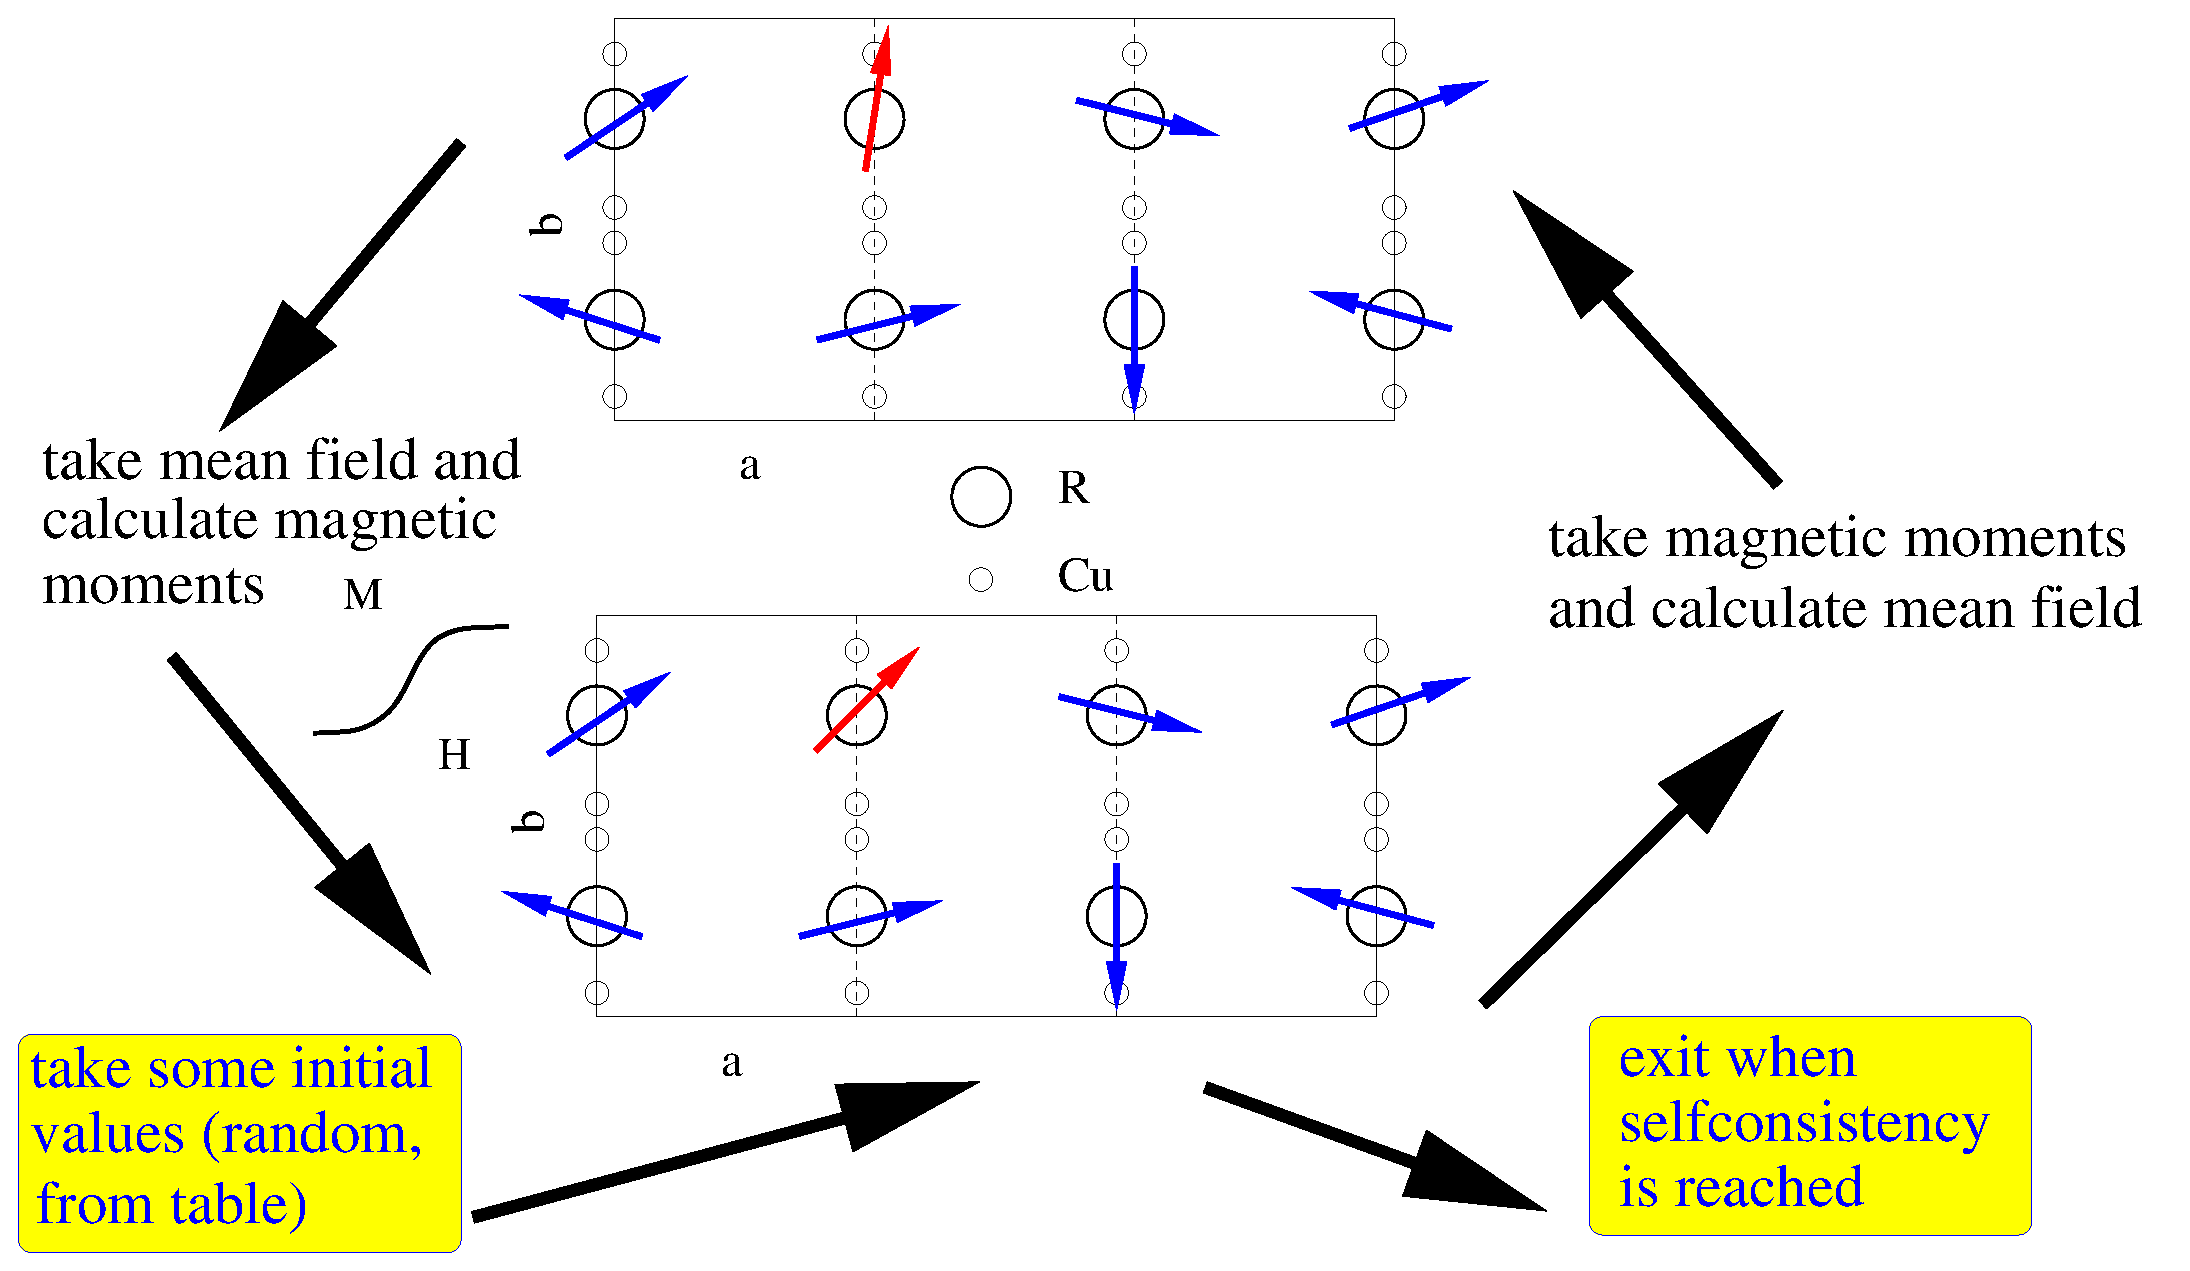
\includegraphics[angle=0,width=0.9\columnwidth]{figsrc/fecalc.eps}
\caption{\label{fecalc}Mean field process of sub {\prg fecalc}.}
\end{figure}

 
\subsubsection{Example {\prg mcphas.ini\index{mcphas.ini}} file for a simple antiferromagnet}

Here is an example of {\prg mcphas.ini\index{mcphas.ini}}, the comments describe the meaning of the different
parameters:

\section{{\prg mcphas} - calculation of thermodynamic properties (Magnetisation, Susceptibility, Specific Heat, Neutron %%@
Diffraction, etc.)}
\label{runmcphas}

In order to perform calculations beyond the capabilities of {\prg cfield\index{cfield}} it is necessary
to use the program {\prg mcphas}. 
\begin{itemize}
\item As a first step it is possible to
calculate the thermodynamic properties such as magnetisation or specific heat
considering only single ion effects. In this case all the exchange parameters
have to be set to zero in {\prg mcphas.j\index{mcphas.j}}. 
\item for more advanced calculations the two - ion interactions have to be
considered and may lead to magnetic order. {\prg mcphas} can perform 
calculations in the ordered state in the following way: for 
a given temperature $T$ and magnetic field $\mbf H$ (vector)
several possible magnetic structures are stabilised
by a mean field algorithm and the free energy is 
calculated. The initial values for this mean-field procedure are
modified by a Monte Carlo process.


The temperature and magnetic field is varied during the calculation
and thereby it is possible to map out the magnetic phase diagram.
\end{itemize}

The program produces a plot of the stabilised magnetic
structures and the magnetisation on screen, the
output files contain additional information 
such as calculated magnetoelastic and  neutron-scattering
data. Several graphic programs easy the visualisation of the
calculated data (section~\ref{graphics}).



\subsection{Input Files}
The program {\prg McPhase} needs the following input files (all in the same directory)
 in order to run:

\begin{enumerate}
\item {\prg mcphas.ini\index{mcphas.ini}}
 - controlling the algorithm
\item {\prg mcphas.j\index{mcphas.j}}
  - lattice and exchange parameters
\item {\prg mcphas.tst\index{mcphas.tst}(optional)}  - test spin configurations
\item {\prg single-ion property files}
\item {\prg directory ./results/}
 - directory where calculated data is stored
\item {\prg directory ./fit} - experimental data for fit (optional)
\end{enumerate}


 All
 of these input files have to be in one directory and the program
has to be started in this directory. The results of the simulation
are then stored in the  subdirectory ./results/, which must exist before starting
the program 
... see directory ./examples/ for some examples.
 In order to prepare these files
for a new calculation it is best to take them from an example, copy the files
to a new directory and make the
modifications  to adapt them to the new problem.

\subsubsection{Example - a simple antiferromagnet}

In the following description of the input files we will always refer
to a simple example: a simple antiferromagnet
on a primitive orthorhombic lattice. The first time user
will thus have a simple example to follow, all corresponding
files are given in the directory {\prg tutorial/03magnetic\_phases\_mcphas/simpleAF}.
 

\subsubsection{{\prg mcphas.ini\index{mcphas.ini}} - controlling the algorithm}
   Initial file containing algorithm control parameters, for instance the range and spacing of
   propagation vectors Q or the number of Monte Carlo trials for initial spin configurations
    - {\em mind}: this
   file is rewritten and reread  when running the program and may be changed by the
   user in order to manipulate the running simulation.

{\prg mcphas.ini\index{mcphas.ini}} consists of several sections:
\begin{description}
\item [MCPHASE RUNTIME CONTROL:] this section contains the parameters
controlling the status of the calculation.
\item [XY PHASEDIAGRAM PARAMETERS:] here the temperature and field range and
step widths of the calculation are specified.
The definition of the x and y
axis in terms of temperature and magnetic field is followed by the
corresponding range and step width. An offset may be given for all
field and temperature values.
Note that for most cases of interest
this offset is zero (T0=0, Ha0=0, Hb0=0, Hc0=0).
 For the simple case of calculating a Temperature-Field phase diagram
 It is just necessary to set xT=1 and give the temperature range by
xmin/xmax/xstep. For field in b direction then just set yHb=1 and 
define the range in ymin/ymax/ystep.
In case of non-orthogonal axes the applied magnetic field
components $Ha, Hb, Hc$ refer to the orthogonal coordinate system
defined with respect to the nonorthogonal lattice $\mbf a,\mbf b,\mbf c$ as
$Hb||\mbf b$, $Hc||(\mbf a \times \mbf b)$ and $Ha$ perpendicular to $Hb$ and $Hc$.

\item [GENERATION OF SPINCONFIGURATIONS:] at the beginning of the program
some initial values of spin configurations are generated from a set of 
propagation vectors. This section defines the range of propagation vectors
and the step width.
Depending on the value of the propagation Q with respect to the primitive reciprocal lattice
1-, 2- or 3-dimensional simulations of magnetic lattices
are possible. It is advisable to 
think carefully about the chosen range and spacing of Q vectors in order
to limit calculation time.
 
For example a good starting point is to begin with a calculation with large
step widths (e.g. 0.1)  covering the Brillouin zone. This should give an idea
of the propagation vectors which are stabilised. An advanced calculation
could then fine tune the propagation and determine its accurate value (using
small step widths in a limited area of the zone).
The verbose option of {\prg mcphas} allows to inspect the propagation vectors
which are actually used in the calculation.
Trick: in order to get a quick overview of the
q-vector range covered by the mcphas\index{mcphas} simulation start mcphas, exit and 
just type {\prg felog ./results/mcphas.qvc} (need {\prg perl,perldl,pdl,pgplot} packages).

In order to limit calculation time, the maximum periodicity
of the magnetic unit cell with respect to the crystallographic unit cell 
(maxqperiod) and the maximum number of spins in the magnetic unit cell 
(maxnofspins) can be limited. Also the maximum number of test spin configurations
in the internal table can be limited (maxnoftestspincf).
A critical feature with respect to calculation time is also the number of
spin configurations which are generated by a random process from a tabulated
SPINCONFIGURATIONS during the calculation. 

In summary the variables in this section are mainly important to adapt the
program to a given computer system with finite speed. They have to be set
to optimise between speed and accuracy of the calculation. In order to
find appropriate values it is best to perform some calculations 
and restrict the parameters step by step if insufficient speed is obtained.
Also the examples included in the program package may serve as starting
points.

\item [PARAMETERS FOR SUB FECALC SELFCONSISTENCY PROCESS:] the most important
procedure in the module {\prg mcphas} is the sub fecalc. In this part of the 
program the self consistent calculation of the magnetic moment configuration
is performed as shown schematically in fig.~\ref{fecalc}. 
In the mean field approximation the Hamiltonian~(\ref{hamilton}) is approximated
by

\begin{equation}
 {\mathcal H}=\sum_n H_{SI}^n + E_{corr}
\end{equation}

with the single ion Hamiltonian (in case of module {\prg so1ion\index{so1ion}})

\begin{equation}
H_{SI}^n=  B_l^m O_{lm}({\mbf J}^n) 
	     - g_{Jn} \mu_B {\mbf J}^n {\mbf H^n_{eff}} 
\end{equation}

and the correction term

\begin{equation}
E_{corr}=\frac{1}{2}\sum_{n} g_{Jn} \mu_B \langle {\mbf J}^n
 \rangle (\mbf H^n_{eff}-\mbf H) 
\end{equation}

and with the mean fields $ \mbf H^n_{eff}$ given by

\begin{equation}\label{meanfield}
\mbf H^n_{eff}=\mbf H + \mbf H^n_{xc}=\mbf H+\sum_{{\mbf G'}n'} \frac{{\mathcal J}
(\mbf r_n-(\mbf G'+\mbf r_{n'}))}{g_{Jn}\mu_B } \langle{\mbf
J}^{n'}\rangle
\end{equation}

These mean fields and the moments $\langle \mbf J^n \rangle$ 
are determined in a self consistent
way. For a given magnetic unit cell and initial configuration 
of magnetic moments
the mean fields are calculated according to equation~(\ref{meanfield}). 
Then, for each
magnetic ion the single ion property module is taken 
and the magnetic moment $\langle \mbf J^n \rangle$ is 
calculated from it's mean field. The mean fields are used again in equation~(\ref{meanfield})
and so on .... until convergence is reached. 
Then, the free energy ($f=-kT\sum_n \ln(z_n) + E_{corr}$ ) 
of the stabilised
configuration is calculated (this is why this sub is called {\prg fecalc}). 
The free energies of a lot of different stabilised configurations have to
be compared in order to find out which configuration has lowest free energy, i.e.
is stable in thermal  equilibrium.

It may happen that this process does
not converge due to bad choice of the initial configuration, therefore a maximum number
of mean field loops has to be given by the user.
The results of a calculation may be significantly influenced by
changing parameters such as the maximum number of iteration loops 
in this section. 
In fact the simulation is always a compromise of calculation time and accuracy: if only
a few initial spin configurations are tried at each (H-T) point, the calculation speed is
fast, however it is possible that the program misses the magnetic structure with the
lowest free energy. The same holds if other critical parameters of the simulation are
restricted too much.
 

\item [OUTPUT OF PHYSICAL PROPERTIES:]
Some options for the output of the calculation can be changed in this section.
\end{description}

\begin{figure}[hb]
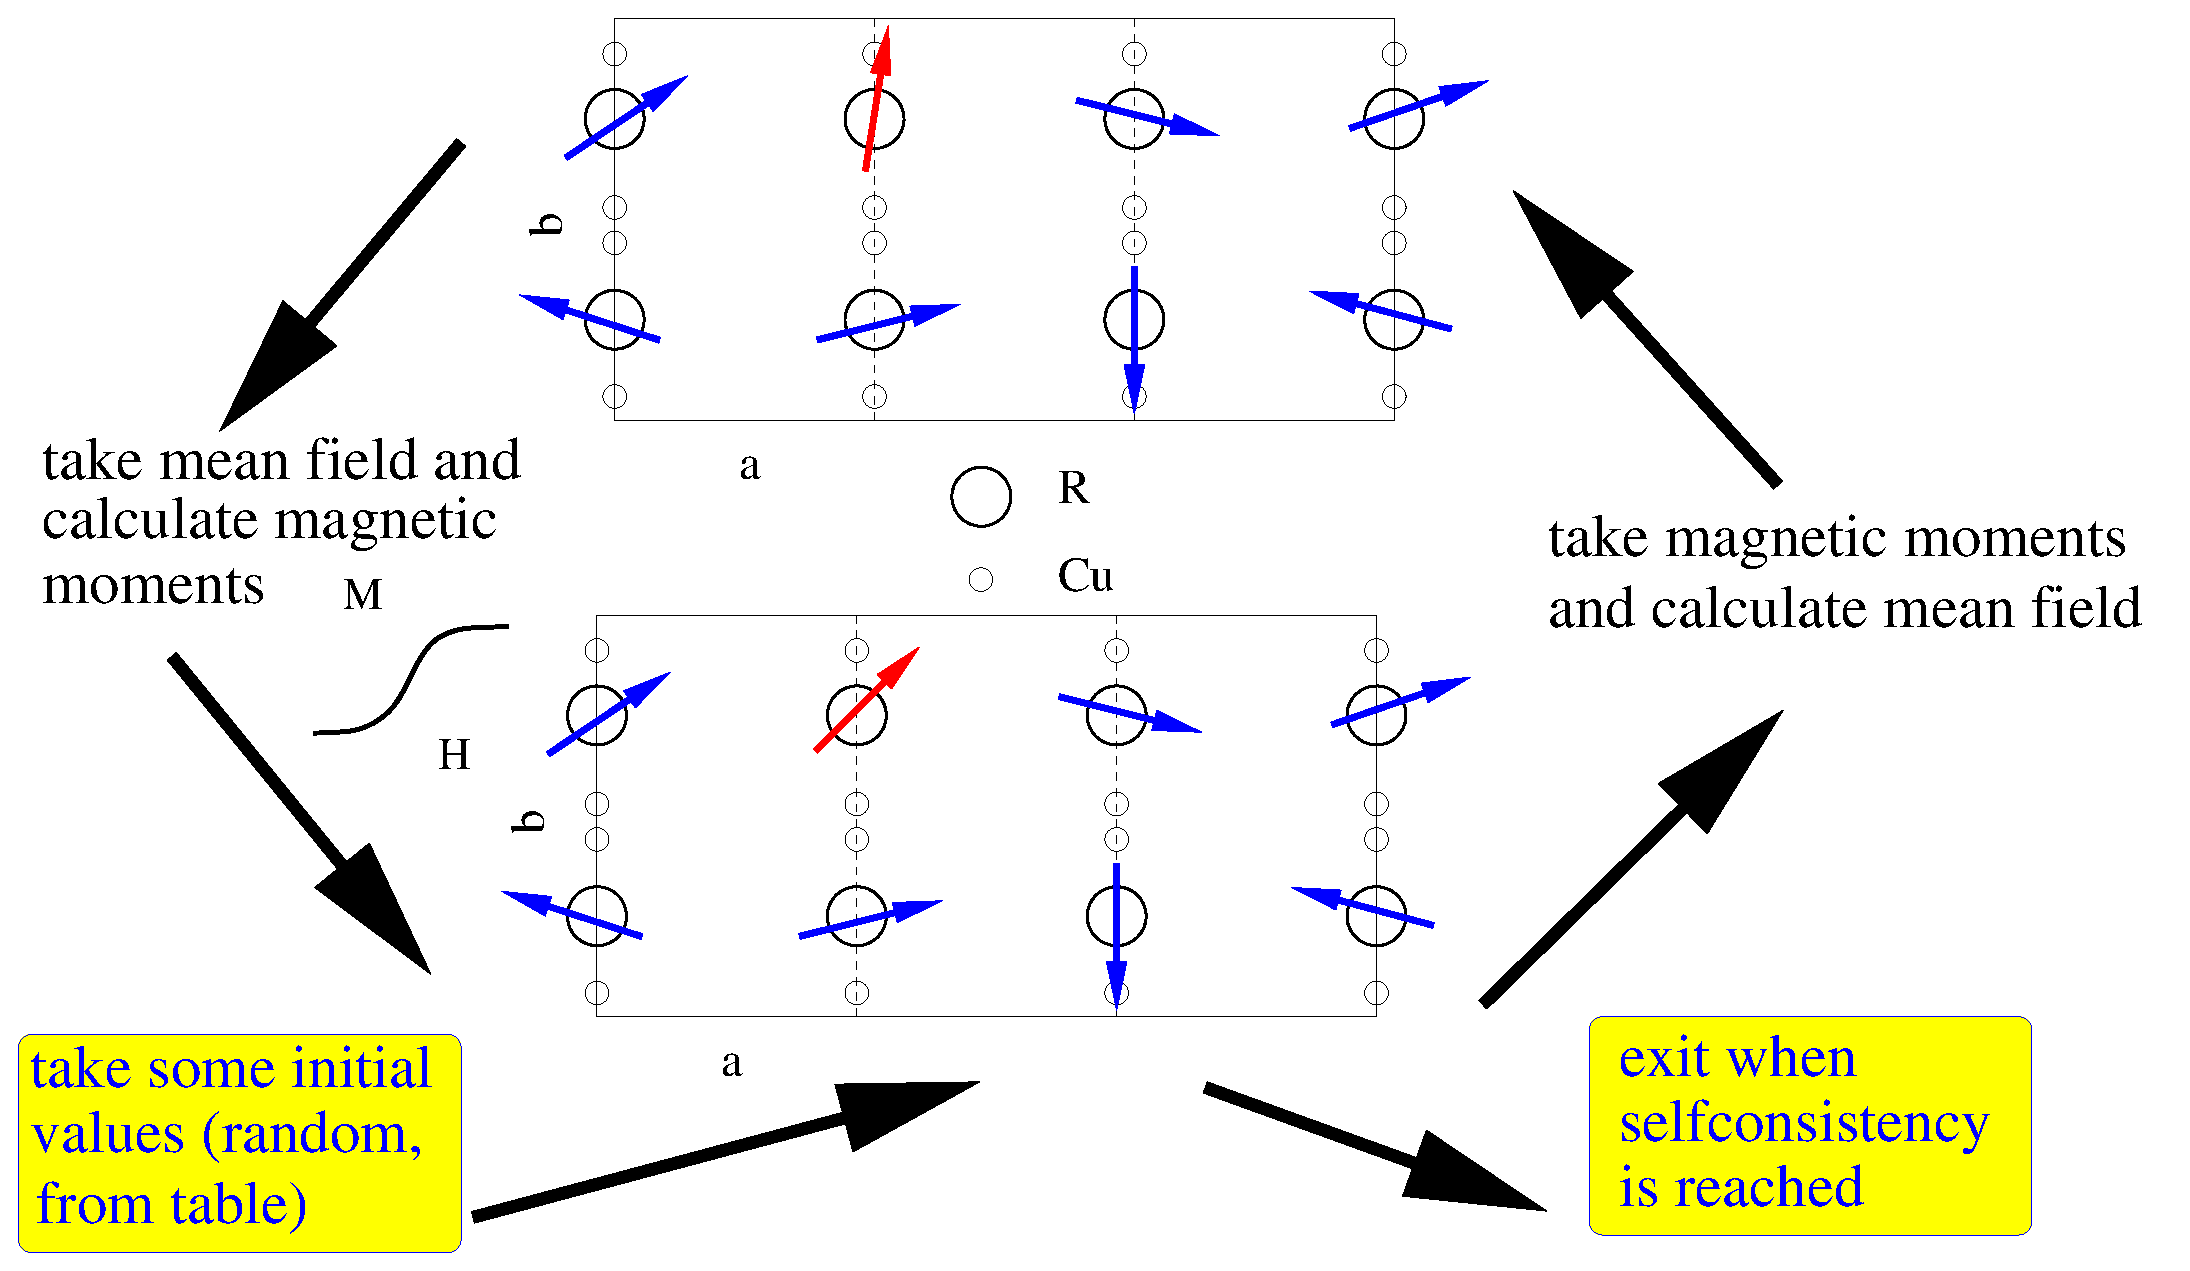
\includegraphics[angle=0,width=0.9\columnwidth]{figsrc/fecalc.eps}
\caption{\label{fecalc}Mean field process of sub {\prg fecalc}.}
\end{figure}

 
\subsubsection{Example {\prg mcphas.ini\index{mcphas.ini}} file for a simple antiferromagnet}

Here is an example of {\prg mcphas.ini\index{mcphas.ini}}, the comments describe the meaning of the different
parameters:

\input{mcphas.ini}



\subsubsection{{\prg mcphas.j\index{mcphas.j}} - lattice and exchange parameters}\label{mcphasj}
This file provides the information about 
the crystallographic
 structure and the magnetic exchange interactions.
For every atom in the crystallographic basis there
has to be given the coordinates, the number of neighbours to be considered, the 
Land\'e factor $g_J$, the single ion property filename and  a set of exchange parameters.
If the exchange parameters (and neighbour positions) are not known for your system, you 
can use the program module {\prg makenn\index{makenn}} (see section \ref{addprog}) to generate 
a list of nearest neighbours and
exchange parameters, currently implemented in {\prg makenn\index{makenn}} are dipolar interactions,
exchange interactions via the Bethe-Slater curve or the RKKY model. Note that in order
to use {\prg makenn\index{makenn}} you have to set up a working {\prg mcphas.j\index{mcphas.j}} file, which may or
may not contain neighbours and interactions.

Use program {\prg addj\index{addj}} to add exchange parameter set stored in different 
such {\prg .j} files (see section~\ref{addprog}).



\begin{description}
\item [Line 1,2:] Comment Lines
\item [Line 3:] lattice constants a,b,c and crystal angles alpha, beta, gamma 
\item [Line 4-6:] primitive lattice vectors
\item [Line 7:] Number of atoms in the primitive crystallographic unit cell ({\prg nofatoms})
\item [Line 8:] a comment line with stars
\item [Line 9:] coordinates  ($d_a$,$d_b$,$d_c$) of 1$^{st}$ magnetic ion in the crystallographic unit cell  with
respect to the lattice vectors $\vec a$,$\vec b$,$\vec c$. The number of neighbours of this 
ion, for which interaction constants are given in the interaction table (nofneighbours). 
If {\prg diagonalexchange}
is set to 0 the 9 components of the exchange tensor are given in column 4-12. 
If {\prg diagonalexchange}
 is 1, only 3 components are given (column 4-6).
If {\prg diagonalexchange}
 is 2, specific components of the exchange tensor can be given in columns 4 onwards. The indices of these components
 must be given in the following line (Line 9a below).
The Land\'e factor of the ion (gJ) and the file name of the corresponding single ion
parameter file (cffilename).
\item [Line 9a:]  If {\prg diagonalexchange=2}, then this line gives the indices of the exchange tensor corresponding to 
 the columns 4 onwards. It must have a variable called {\prg indexexchange} followed by a list of names of components of the interaction
 tensor separated by space. E.g.
 \verb|  #! indexexchange= JaJb JbJc  | 
means column 4 gives the the interaction constant between the
 first angular momentum component of the current ion with the second angular momentum component of its neighbour, whilst 
 column 5 has the interaction constant between the second angular momentum component of this ion with the third component of its
 neighbour. Alternatively, pairs of numbers may be given, as in \verb|  #! indexexchange= 1,2 2,3  |
 Additionally another parameter {\prg symmetricexchange} can be set to 1, where the value in each column is also used 
 for the transposed tensor component. Thus \verb|  #! symmetricexchange=1 indexexchange= JaJb  | is the same as \\
 \verb|  #! indexexchange= JaJb JbJa  | where the 4th and 5th column are the same.
\item [Line 10:]  Comment line
\item [Line 11-(10+nofneighbours):] Interaction table for ion number 1.   
Note: the neighbour coordinates (column 1-3) are given with respect to the lattice vectors
$\vec a$,$\vec b$,$\vec c$. The program then calculates from these values the coordinates
with respect to the primitive lattice $\vec r_1$,~$\vec r_2$,~$\vec r_3$.
($ d_a \vec a + d_b \vec b + d_c \vec c = d_1 \vec r_1 + d_2 \vec r_2 + d_3 \vec r_3$).
Column 4,5,6 \dots contain the components of the interaction tensor $\stackrel{=}{\mathcal J}$. 
Note that in case of non-orthogonal axes the 
components of the moments and the interaction tensor $Ja, Jb, Jc, Jaa, Jbb, Jcc, Jab ...$ 
refer to the orthogonal coordinate system
defined with respect to the nonorthogonal lattice $\vec a,\vec b,\vec c$ as
$Jb||\vec b$, $Jc||(\vec a \times \vec b)$ and $Ja$ perpendicular to $Jb$ and $Jc$.
\item [Line (11+nofneighbours) - end:] for each ion in the unit cell line 8 - (10+nofneighbours)
are repeated.
\end{description}


\vspace{0.5cm}

{\small {\bf Information for experienced users:}
\begin{description}
\item[\prg mcphas.jjj:]
format of exchange parameter file, which only needs a reduced set of exchange
parameters in the input file. Using the program {\prg jjj2j} the file can be transformed
to {\prg mcphas.j\index{mcphas.j}} by adding lines for all the equivalent neighbours. The format definition
of {\prg mcphas.jjj} is the same as {\prg mcphas.j\index{mcphas.j}}, however each line denotes several
equivalent neighbour atoms (instead of only one in {\prg mcphas.j\index{mcphas.j}}) according to the
 following rules:
\begin{itemize}
\item If a nonzero coordinate $d_a$ (or $d_b$,$d_c$) in the interaction table
 corresponds to it's value at the nearest
 lattice point of the primitive lattice,
  additional interactions of the same size
with  neighbours with coordinate $-d_a$ (or $-d_b$,$-d_c$, respectively)
are taken into account. This
holds for each of the three coordinates $d_a$,$d_b$ and $d_c$
 resulting in a maximum
number of 8 equivalent neighbours per line in the interaction table.
\item If the value of $d_a$ (or $d_b$,$d_c$) is zero or differs
from it's value at the nearest lattice point of the primitive lattice, it is 
changed to the value at the nearest lattice point and {\bf no} interaction 
with  neighbours with coordinates $-d_a$ (or $-d_b$,$-d_c$) is
 taken into account. If such
 interaction is needed it may be given in a different line and may
have different magnitude. In this way also crystallographic lattices
with no mirror symmetry may be described.
\end{itemize}
\item[\prg mcphas.coq:]   exchange parameters etc [ in old format]...see examples for details, use {\prg coq2jjj} to 
transform {\prg mcphas.coq} to {\prg mcphas.jjj} format
\end{description}

}


\subsubsection{Example {\prg mcphas.j\index{mcphas.j}} file for a simple antiferromagnet}

Here are example files of a tetragonal antiferromagnet with nearest neighbour interactions, all
files are equivalent:

{\small
\begin{verbatim} 
# simple antiferromagnet 
#<!--mcphase.mcphas.j-->
#***************************************************************
# Lattice Constants (A)
#! a=4.3843 b=4.3843 c=2.4194 alpha=  90 beta=  90 gamma=  90
#! r1a=   1 r2a=   0 r3a=   0
#! r1b=   0 r2b=   1 r3b=   0   primitive lattice vectors [a][b][c]
#! r1c=   0 r2c=   0 r3c=   1
#! nofatoms=1  nofcomponents=3  number of atoms in primitive unit cell/number of components of each spin
# ****************************************************************************
#! da=  0 [a] db=  0 [b] dc=  0 nofneighbours=2 diagonalexchange=0 gJ=0.857143 cffilename=Ce3p.sipf
# da[a] db[b] dc[c] Jaa[meV] Jbb[meV] Jcc[meV] Jab[meV] Jba[meV] Jac[meV] Jca[meV] Jbc[meV] Jcb[meV]
+0	+0	+1	-0.1	-0.1	-0.1   0  0  0  0  0  0
+0	+0	-1	-0.1	-0.1	-0.1   0  0  0  0  0  0
#\end{verbatim}
}

Using diagonalexchange this may be shortened to

{\small
\begin{verbatim} 
# simple antiferromagnet 
#<!--mcphase.mcphas.j-->
#***************************************************************
# Lattice Constants (A)
#! a=4.3843 b=4.3843 c=2.4194 alpha=  90 beta=  90 gamma=  90
#! r1a=   1 r2a=   0 r3a=   0
#! r1b=   0 r2b=   1 r3b=   0   primitive lattice vectors [a][b][c]
#! r1c=   0 r2c=   0 r3c=   1
#! nofatoms=1  nofcomponents=3  number of atoms in primitive unit cell/number of components of each spin
# ****************************************************************************
#! da=  0 [a] db=  0 [b] dc=  0 nofneighbours=2 diagonalexchange=1 gJ=0.857143 cffilename=Ce3p.sipf
# da[a] db[b] dc[c] Jaa[meV] Jbb[meV] Jcc[meV] Jab[meV] Jba[meV] Jac[meV] Jca[meV] Jbc[meV] Jcb[meV]
+0	+0	+1	-0.1	-0.1	-0.1   
+0	+0	-1	-0.1	-0.1	-0.1   
#\end{verbatim}
}

with indexexchange option the sequence of two ion interaction parameters can be changed and
zero parameters may be omitted:

{\small
\begin{verbatim} 
# simple antiferromagnet 
#<!--mcphase.mcphas.j-->
#***************************************************************
# Lattice Constants (A)
#! a=4.3843 b=4.3843 c=2.4194 alpha=  90 beta=  90 gamma=  90
#! r1a=   1 r2a=   0 r3a=   0
#! r1b=   0 r2b=   1 r3b=   0   primitive lattice vectors [a][b][c]
#! r1c=   0 r2c=   0 r3c=   1
#! nofatoms=1  nofcomponents=3  number of atoms in primitive unit cell/number of components of each spin
# ****************************************************************************
#! da=  0 [a] db=  0 [b] dc=  0 nofneighbours=2 diagonalexchange=2 gJ=0.857143 cffilename=Ce3p.sipf
# da[a] db[b] dc[c] Jaa[meV] Jbb[meV] Jcc[meV] Jab[meV] Jba[meV] Jac[meV] Jca[meV] Jbc[meV] Jcb[meV]
#! indexexchange = JaJa JaJc JcJa JbJb JcJc
+0	+0	+1	-0.1 0 0 -0.1	-0.1  
+0	+0	-1	-0.1 0 0 -0.1	-0.1  
#\end{verbatim}
}

{\small
\begin{verbatim} 
# simple antiferromagnet 
#<!--mcphase.mcphas.j-->
#***************************************************************
# Lattice Constants (A)
#! a=4.3843 b=4.3843 c=2.4194 alpha=  90 beta=  90 gamma=  90
#! r1a=   1 r2a=   0 r3a=   0
#! r1b=   0 r2b=   1 r3b=   0   primitive lattice vectors [a][b][c]
#! r1c=   0 r2c=   0 r3c=   1
#! nofatoms=1  nofcomponents=3  number of atoms in primitive unit cell/number of components of each spin
# ****************************************************************************
#! da=  0 [a] db=  0 [b] dc=  0 nofneighbours=2 diagonalexchange=2 gJ=0.857143 cffilename=Ce3p.sipf
# da[a] db[b] dc[c] Jaa[meV] Jbb[meV] Jcc[meV] Jab[meV] Jba[meV] Jac[meV] Jca[meV] Jbc[meV] Jcb[meV]
#! indexexchange = 1,1 1,3, 3,1 2,2 3,3
+0	+0	+1	-0.1 0 0 -0.1	-0.1  
+0	+0	-1	-0.1 0 0 -0.1	-0.1  
#\end{verbatim}
}


using symmetricexchange together with indexexchange will assume that the interaction tensor is symmetic and 
only half of it may be given:

{\small
\begin{verbatim} 
# simple antiferromagnet 
#<!--mcphase.mcphas.j-->
#***************************************************************
# Lattice Constants (A)
#! a=4.3843 b=4.3843 c=2.4194 alpha=  90 beta=  90 gamma=  90
#! r1a=   1 r2a=   0 r3a=   0
#! r1b=   0 r2b=   1 r3b=   0   primitive lattice vectors [a][b][c]
#! r1c=   0 r2c=   0 r3c=   1
#! nofatoms=1  nofcomponents=3  number of atoms in primitive unit cell/number of components of each spin
# ****************************************************************************
#! da=  0 [a] db=  0 [b] dc=  0 nofneighbours=2 diagonalexchange=2 gJ=0.857143 cffilename=Ce3p.sipf
# da[a] db[b] dc[c] Jaa[meV] Jbb[meV] Jcc[meV] Jab[meV] Jba[meV] Jac[meV] Jca[meV] Jbc[meV] Jcb[meV]
#! symmetricexchange=1 indexexchange = JaJa JaJc JbJb JcJc
+0	+0	+1	-0.1 0  -0.1	-0.1  
+0	+0	-1	-0.1 0  -0.1	-0.1  
#\end{verbatim}
}


\subsubsection{Single Ion Property Input Files}\label{sifile}

In order to speed up calculations or treat special problems a large 
variety of single ion modules is available. This includes the
option to load a user written single ion module. Details are 
given in chapter~\ref{simod}.

The first time user of {\prg McPhase} should use the module {\prg so1ion}\index{so1ion} and 
create an appropriate single ion property input file as described in
section \ref{cf1ion}. A good starting point are several examples
given in directory {\prg examples}.


\subsubsection{Example single ion property file  for a simple antiferromagnet}

Here is an example file {\prg mcphas.cf1} describing the anisotropy of a 
simple antiferromagnet with Ce atoms having basal plane anisotropy. Note the
axis convention xyz$||$abc, in case of non-orthogonal axes the convention 
is $y||\vec b$, $z||(\vec a \times \vec b)$ and $x$ perpendicular to $y$ and $z$.


\input{mcphas.cf1}

\subsubsection{{\prg mcphas.tst\index{mcphas.tst}} - input file of test spin-configurations (optional)}
This file is optional and contains
some test momentum configurations to be used for the calculation
             of the free energy. Mind that
\begin{itemize}
\item  in the file header the number of atoms in the primitive
       crystallographic unit cell and the number of components
       of the spin vector have to be given.
\item  at the end of the
 file there must be no empty lines !
\end{itemize}

The momentum - configurations tables always refer to spins sitting on
the primitive lattice ${\mbf r}_i$. If more than one atom is in
the primitive basis, the momentum gets $3n$ components ($n=$ number
of atoms in the crystallographic basis). See {\prg ./examples/ndcu2b\_new/} for
examples of a two atom basis. Units of these tables are that of total 
angular momentum $<J>$.

\subsubsection{Example {\prg mcphas.tst\index{mcphas.tst}} file  for a simple antiferromagnet}

Here is the file {\prg mcphas.tst\index{mcphas.tst}} for the simple antiferromagnet example
describing some spin configurations
to be used as starting values for the mean field process:

\input{mcphas.tst}
Note, in case of non-orthogonal axes the convention 
is $mb||\vec b$, $mc||(\vec a \times \vec b)$ and $ma$ perpendicular to $mb$ and $mc$.

\subsubsection{subdirectory {\prg ./results} - directory where calculated data is stored}

In order to be able to save the results of a calculation the directory {\prg ./results} has to
exist. Mind that all files in this directory will be overwritten without warning. 

\subsubsection{subdirectory {\prg ./fit} - experimental data for fit (optional) } 

In order that {\prg McPhase} can calculate the standard deviation between
 experimental data and the results of the simulation, some experimental data
 can be given in the subdirectory {\prg ./fit}. The filenames and the data-format
 are the same as the output files of {\prg McPhas}, e.g. {\prg mcphas.fum}, {\prg mcphas.hkl}
 etc. {\prg McPhase} looks into the directory {\prg ./fit} and if it finds any
 of these files, the standard deviation is increased correspondingly. 

What measurement data can be used to calculate a standard deviation ?

\begin{description}
\item[{\prg mcphas.fum}] if given in column 11, 12, 13 in {\prg ./fit/mcphas.fum} the
            magnetisation in the $a$, $b$ and $c$ direction is used for calculation
	    of the standard deviation sta. The standard deviation is calculated
	    as ${\rm sta}=\sum_{\rm data points i} ({\mbf m}_i^{calc}-{\mbf m}_i^{meas})^2$.
	    All three components of the magnetic moment have to be given and are used.

\end{description}

Note that the measured data has to be given in those (H-T) points which are 
calculated by mcphas\index{mcphas} in order to be used by the program to increase {\prg sta}.
It is usually most effective to fit only few data points, because a large set
of data points will not improve the quality of the fit and only require a large
amount of calculation time.



\subsection{Starting a simulation}
\label{start}

To start the simulation goto the directory containing the
input files {\prg mcphas.ini, mcphas.j, etc. } and type

\begin{description}
\item[\prg mcphas] to run the program generating stepwise $H-T$ values 
              in a loop given by {\prg mcphas.ini\index{mcphas.ini}} (you can also press the
              symbol in the {\prg McPhase - Explorer} window).
\item[\prg mcphas\index{mcphas} [file]]  to run the program with an input file --   
             {\prg file} contains T ha hb hc values to be calculated 
             if [file] is not given, xmin xmax xstep (xT xHa xHb xHc)
             ymin ymax ystep (yT yHa yHb yHc) is read from file {\prg mcphas.ini\index{mcphas.ini}}
	     and phase diagram is calculated
\item[\prg mcphas\index{mcphas} -h]  to  print help and version of {\prg McPhas}.
\item[\prg mcphas\index{mcphas} -stamax 14]  end mcphas\index{mcphas} if standard deviation exceeds 14.
\item[\prg mcphas\index{mcphas} -a] avoid overwriting output files in results, append new results to existing files
\item[\prg mcphas\index{mcphas} -v]  to  enable verbose mode with lots of messages of {\prg McPhas}. Specifically
the verbose mode enables the following features:
  \begin{itemize}
			          \item more information is printed out, 
			          \item the q-vectors file {\prg ./results/mcphas.qvc} will contain 
				    the explicit spin configurations
			          \item the display\index{display} on screen (ghostview window using 
				     {\prg ./results/.sps.eps}) will be updated not only 
				    when a H-T point has been finished but always 
				    when a structure with smaller free energy 
				    has been stabilised
  \end{itemize}
\item[\prg mcphasit\index{mcphas}] to start mcphase in commandline mode without opening any window
\end{description}

\vspace{1cm}
{\em Exercises:}
\begin{itemize}
\item Look at the input files for {\prg McPhase} given in the directory
{\prg examples/ndcu2b\_new}.  How many atoms are contained in the crystallographic basis ?
\item
Start the simulation by typing the command {\prg mcphas}.
\end{itemize}



\subsection{Options for a running simulation}
... when the program is running, the options in the main window
can be changed. Pressing ''displayall'' displays the current spin-configuration
at each iteration step. Pressing ''log fe vs Q'' appends free energy vs Q
data to {\prg mcphas.log} for every ($T-H$) point.


The file {\prg ./results/.spins.eps} is used to show the information about the currently calculated
spin structure on the screen using the postscript file viewer ghostview.

The file {\prg ./results/.mcphas.fum} contains the information of the magnetisation curve
which is currently calculated. This information is automatically displayed on the screen.


The program {\prg display} (see section \ref{display}) can be used 
for the online display\index{display} of any other
curve(s).


\subsection{Output Files - {\prg mcphas.qvc,phs,sps,mf,fum,j1...,xyt,hkl} }\label{outputfiles}
 (in directory ./results/ after a simulation run) 

\begin{figure}[htb]%h=here, t=top, b=bottom, p=separate figure page
\begin{center}\leavevmode
\includegraphics[angle=0, width=0.3\textwidth]{figsrc/magnetization_ndcu2.ps}
\end{center}
\caption{Calculated magnetisation of NdCu$_2$ for field parallel to the orthorhombic $b$-direction.}
\label{magnetization}
\end{figure}

\begin{figure}[htb]%h=here, t=top, b=bottom, p=separate figure page
\begin{center}\leavevmode
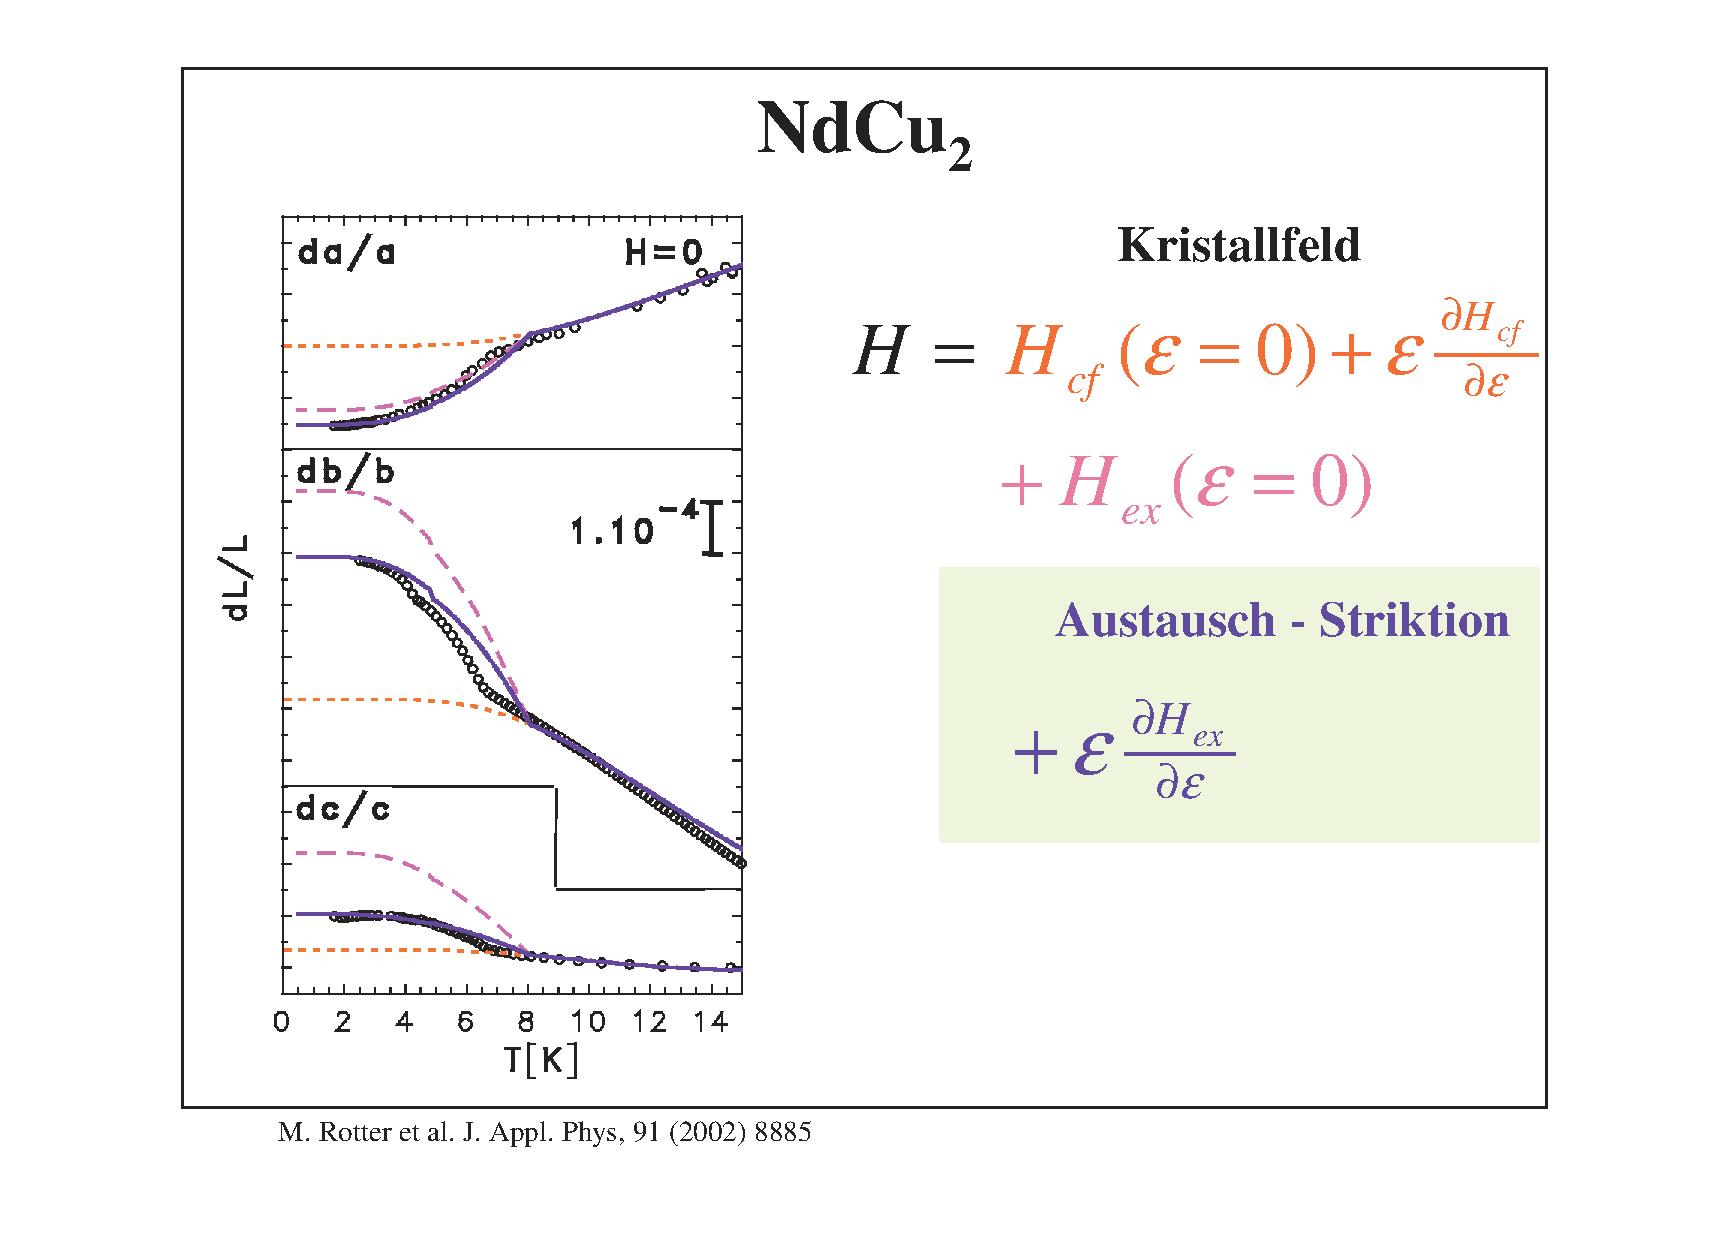
\includegraphics[angle=0, width=0.8\textwidth]{figsrc/magnetostriction_ndcu2.eps}
\end{center}
\caption{Calculated spontaneous magnetostriction of NdCu$_2$.}
\label{magnetostrictiongraphic}
\end{figure}

\begin{description}
\item [\prg mcphas.qvc]    the set of test q-vectors used for calculation of free energy.
                           Components of these q vectors refer to the reciprocal lattice $\vec a^*,\vec b^*,\vec c^*$.
\item [\prg mcphas.phs]    spin-configuration table of different types of spin-configurations. 
                            Note, in case of non-orthogonal axes the convention in these tables 
                            is $mb||\vec b$, $mc||(\vec a \times \vec b)$ and $ma$ perpendicular to $mb$ and $mc$.

                           {\em Note}: 
                           there is no natural criteria for deciding, if one spin-configuration is
			   different from another one. Therefore the list of ''different''
			   spin-configurations is dependent on the meaning of ''different''.
			   
			   The program {\prg McPhase} decides whether a spin-configuration is
			   different from another by a simple criteria, namely by the
			   angle between the spins. Comparing two spin configurations it calculates
			   the angle between corresponding spins and if for one spin the
			   angle is not small, the configuration is treated as a different
			   configuration. Therefore for example a ferromagnet with moments
			   in $a$ has a different spin configuration than a ferromagnet with
			   moments in $b$ direction. 
\item [\prg mcphas.sps]    $T-H$ dependence of spin-configuration. The spin configurations stored in this
                           file may be displayed using the program {\prg spins\index{spins}}, an example is given
			   in figure~\ref{spingraphic}.
                            Note, in case of non-orthogonal axes the convention for applied field $Ha, Hb,Hc$ and
                            also for the moment components $ma, mb, mc$ in these tables 
                            is $mb||\vec b$, $mc||(\vec a \times \vec b)$ and $ma$ perpendicular to $mb$ and $mc$.

\item [\prg mcphas.mf]     $T-H$ dependence of exchange field configuration, stored as $g_J \mu_B H_{xc}(i)$(unit is in meV)
                            for i=1,2,...,number of spins in magnetic unit cell.
                            Note, in case of non-orthogonal axes the convention for applied field $Ha, Hb,Hc$ and
                            also for the mean field components in these tables 
                            is $Hb||\vec b$, $Hc||(\vec a \times \vec b)$ and $Ha$ perpendicular to $Hb$ and $Hc$.
\item [\prg mcphas.fum]    free energy, magnetic energy (the derivative with respect to temperature gives the specific %%@
heat),
                           magnetisation data and (if cfield is used with higher order interactions)
                           expectation values of the Stevens Operators $<O_l^m>$ . As an example for the information
			   contained in this file the calculated magnetisation and magnetostriction of NdCu$_2$ is shown in
			   figures~\ref{magnetization} and ~\ref{magnetizationgraphic}.
                            Note, in case of non-orthogonal axes the convention for applied field $Ha, Hb,Hc$ and
                            also for the magnetisation components $ma,mb,mc$ in these tables 
                            is $Hb||\vec b$, $Hc||(\vec a \times \vec b)$ and $Ha$ perpendicular to $Hb$ and $Hc$.

\item [\prg mcphas1.j1 .j1 .j2 ...] 
               spin-spin correlation functions for sub-lattice 1 neighbour 1 2 ...
	       (linear combination is proportional to magnetostriction)
	       The spin-spin correlation functions for neighbour $k$ are defined by
	       the following sum of dyadic products:

	       \begin{equation}
	        \frac{1}{n}\sum_{s=1}^n <{\mbf J}^s> \times  <{\mbf J}^{s+k}>
	       \end{equation}
	       with $n$ being the number of moments in the magnetic unit cell.
	       Single ion and two-ion magnetostriction can be calculated using the $<O_l^m>$ and the
	       spin-spin correlation functions. As an example the magnetostriction analysis of
	       NdCu$_2$ is shown in figure~\ref{magnetostrictiongraphic}. For details 
             please refer to~\cite{rotter02-8885}.
                            Note, in case of non-orthogonal axes the convention for applied field $Ha, Hb,Hc$ and
                            also for the moment components in these tables 
                            is $Hb||\vec b$, $Hc||(\vec a \times \vec b)$ and $Ha$ perpendicular to $Hb$ and $Hc$.
\item [\prg mcphas.xyt]    phase diagram as x,y,T, H, phase-number j according to spin-configuration table
               given in mcphas.phs, a periodicity key, nettomoments <J>.
 Figure~\ref{phasediagramgraphic}
	       shows the phase diagram of NdCu$_2$ for magnetic fields parallel to the orthorhombic $b$-direction.
                            Note, in case of non-orthogonal axes the convention for applied field $Ha, Hb,Hc$ 
                             in these tables 
                            is $Hb||\vec b$, $Hc||(\vec a \times \vec b)$ and $Ha$ perpendicular to $Hb$ and $Hc$.
\item [\prg mcphas.hkl]    calculated (unpolarised) neutron diffraction data (the calculated magnetic intensities
    correspond to the magnetic structure + Polarisation factor. The
    Lorentz-factor , magnetic form factor and  instrumental corrections are not calculated.)
 As an example figure~\ref{neutintgraphic}
    shows the calculated temperature dependence of magnetic amplitudes for NdCu$_2$.
                           $h,k,l$ refer to the reciprocal lattice $\vec a^*,\vec b^*,\vec c^*$.
                            Note, in case of non-orthogonal axes the convention for applied field $Ha, Hb,Hc$ 
                             in these tables 
                            is $Hb||\vec b$, $Hc||(\vec a \times \vec b)$ and $Ha$ perpendicular to $Hb$ and $Hc$.
    
\item [\prg mcphasa.hkl]    Fourier Transform of the $a$-component of the magnetic Moments.
                           $h,k,l$ refer to the reciprocal lattice $\vec a^*,\vec b^*,\vec c^*$.
                            Note, in case of non-orthogonal axes the convention for applied field $Ha, Hb,Hc$ and
                            the magnetic moment component in these tables 
                            is $Hb||\vec b$, $Hc||(\vec a \times \vec b)$ and $Ha$ perpendicular to $Hb$ and $Hc$.
\item [\prg mcphasb.hkl]    Fourier Transform of the $b$-component of the magnetic Moments.
                           $h,k,l$ refer to the reciprocal lattice $\vec a^*,\vec b^*,\vec c^*$.
                            Note, in case of non-orthogonal axes the convention for applied field $Ha, Hb,Hc$ and
                            the magnetic moment component in these tables 
                            is $Hb||\vec b$, $Hc||(\vec a \times \vec b)$ and $Ha$ perpendicular to $Hb$ and $Hc$.
\item [\prg mcphasc.hkl]    Fourier Transform of the $c$-component of the magnetic Moments.
                           $h,k,l$ refer to the reciprocal lattice $\vec a^*,\vec b^*,\vec c^*$.
                            Note, in case of non-orthogonal axes the convention for applied field $Ha, Hb,Hc$ and
                            the magnetic moment component in these tables 
                            is $Hb||\vec b$, $Hc||(\vec a \times \vec b)$ and $Ha$ perpendicular to $Hb$ and $Hc$.
\end{description} 

\vspace{1cm}
{\em Exercises:}
\begin{itemize}
\item Look at the output files of {\prg McPhase}  in the directory
{\prg examples/ndcu2b\_new/results}.  At which magnetic field
the ferromagnetically aligned state is achieved (at $T=$2~K)?
\item
What is the propagation vector in the different antiferromagnetic phases at $T=$2~K ?
\end{itemize}





\subsubsection{{\prg mcphas.j\index{mcphas.j}} - lattice and exchange parameters}\label{mcphasj}
This file provides the information about 
the crystallographic
 structure and the magnetic exchange interactions.
For every atom in the crystallographic basis there
has to be given the coordinates, the number of neighbours to be considered, the 
Land\'e factor $g_J$, the single ion property filename and  a set of exchange parameters.
If the exchange parameters (and neighbour positions) are not known for your system, you 
can use the program module {\prg makenn\index{makenn}} (see section \ref{addprog}) to generate 
a list of nearest neighbours and
exchange parameters, currently implemented in {\prg makenn\index{makenn}} are dipolar interactions,
exchange interactions via the Bethe-Slater curve or the RKKY model. Note that in order
to use {\prg makenn\index{makenn}} you have to set up a working {\prg mcphas.j\index{mcphas.j}} file, which may or
may not contain neighbours and interactions.

Use program {\prg addj\index{addj}} to add exchange parameter set stored in different 
such {\prg .j} files (see section~\ref{addprog}).



\begin{description}
\item [Line 1,2:] Comment Lines
\item [Line 3:] lattice constants a,b,c and crystal angles alpha, beta, gamma 
\item [Line 4-6:] primitive lattice vectors
\item [Line 7:] Number of atoms in the primitive crystallographic unit cell ({\prg nofatoms})
\item [Line 8:] a comment line with stars
\item [Line 9:] coordinates  ($d_a$,$d_b$,$d_c$) of 1$^{st}$ magnetic ion in the crystallographic unit cell  with
respect to the lattice vectors $\vec a$,$\vec b$,$\vec c$. The number of neighbours of this 
ion, for which interaction constants are given in the interaction table (nofneighbours). 
If {\prg diagonalexchange}
is set to 0 the 9 components of the exchange tensor are given in column 4-12. 
If {\prg diagonalexchange}
 is 1, only 3 components are given (column 4-6).
If {\prg diagonalexchange}
 is 2, specific components of the exchange tensor can be given in columns 4 onwards. The indices of these components
 must be given in the following line (Line 9a below).
The Land\'e factor of the ion (gJ) and the file name of the corresponding single ion
parameter file (cffilename).
\item [Line 9a:]  If {\prg diagonalexchange=2}, then this line gives the indices of the exchange tensor corresponding to 
 the columns 4 onwards. It must have a variable called {\prg indexexchange} followed by a list of names of components of the interaction
 tensor separated by space. E.g.
 \verb|  #! indexexchange= JaJb JbJc  | 
means column 4 gives the the interaction constant between the
 first angular momentum component of the current ion with the second angular momentum component of its neighbour, whilst 
 column 5 has the interaction constant between the second angular momentum component of this ion with the third component of its
 neighbour. Alternatively, pairs of numbers may be given, as in \verb|  #! indexexchange= 1,2 2,3  |
 Additionally another parameter {\prg symmetricexchange} can be set to 1, where the value in each column is also used 
 for the transposed tensor component. Thus \verb|  #! symmetricexchange=1 indexexchange= JaJb  | is the same as \\
 \verb|  #! indexexchange= JaJb JbJa  | where the 4th and 5th column are the same.
\item [Line 10:]  Comment line
\item [Line 11-(10+nofneighbours):] Interaction table for ion number 1.   
Note: the neighbour coordinates (column 1-3) are given with respect to the lattice vectors
$\vec a$,$\vec b$,$\vec c$. The program then calculates from these values the coordinates
with respect to the primitive lattice $\vec r_1$,~$\vec r_2$,~$\vec r_3$.
($ d_a \vec a + d_b \vec b + d_c \vec c = d_1 \vec r_1 + d_2 \vec r_2 + d_3 \vec r_3$).
Column 4,5,6 \dots contain the components of the interaction tensor $\stackrel{=}{\mathcal J}$. 
Note that in case of non-orthogonal axes the 
components of the moments and the interaction tensor $Ja, Jb, Jc, Jaa, Jbb, Jcc, Jab ...$ 
refer to the orthogonal coordinate system
defined with respect to the nonorthogonal lattice $\vec a,\vec b,\vec c$ as
$Jb||\vec b$, $Jc||(\vec a \times \vec b)$ and $Ja$ perpendicular to $Jb$ and $Jc$.
\item [Line (11+nofneighbours) - end:] for each ion in the unit cell line 8 - (10+nofneighbours)
are repeated.
\end{description}


\vspace{0.5cm}

{\small {\bf Information for experienced users:}
\begin{description}
\item[\prg mcphas.jjj:]
format of exchange parameter file, which only needs a reduced set of exchange
parameters in the input file. Using the program {\prg jjj2j} the file can be transformed
to {\prg mcphas.j\index{mcphas.j}} by adding lines for all the equivalent neighbours. The format definition
of {\prg mcphas.jjj} is the same as {\prg mcphas.j\index{mcphas.j}}, however each line denotes several
equivalent neighbour atoms (instead of only one in {\prg mcphas.j\index{mcphas.j}}) according to the
 following rules:
\begin{itemize}
\item If a nonzero coordinate $d_a$ (or $d_b$,$d_c$) in the interaction table
 corresponds to it's value at the nearest
 lattice point of the primitive lattice,
  additional interactions of the same size
with  neighbours with coordinate $-d_a$ (or $-d_b$,$-d_c$, respectively)
are taken into account. This
holds for each of the three coordinates $d_a$,$d_b$ and $d_c$
 resulting in a maximum
number of 8 equivalent neighbours per line in the interaction table.
\item If the value of $d_a$ (or $d_b$,$d_c$) is zero or differs
from it's value at the nearest lattice point of the primitive lattice, it is 
changed to the value at the nearest lattice point and {\bf no} interaction 
with  neighbours with coordinates $-d_a$ (or $-d_b$,$-d_c$) is
 taken into account. If such
 interaction is needed it may be given in a different line and may
have different magnitude. In this way also crystallographic lattices
with no mirror symmetry may be described.
\end{itemize}
\item[\prg mcphas.coq:]   exchange parameters etc [ in old format]...see examples for details, use {\prg coq2jjj} to 
transform {\prg mcphas.coq} to {\prg mcphas.jjj} format
\end{description}

}


\subsubsection{Example {\prg mcphas.j\index{mcphas.j}} file for a simple antiferromagnet}

Here are example files of a tetragonal antiferromagnet with nearest neighbour interactions, all
files are equivalent:

{\small
\begin{verbatim} 
# simple antiferromagnet 
#<!--mcphase.mcphas.j-->
#***************************************************************
# Lattice Constants (A)
#! a=4.3843 b=4.3843 c=2.4194 alpha=  90 beta=  90 gamma=  90
#! r1a=   1 r2a=   0 r3a=   0
#! r1b=   0 r2b=   1 r3b=   0   primitive lattice vectors [a][b][c]
#! r1c=   0 r2c=   0 r3c=   1
#! nofatoms=1  nofcomponents=3  number of atoms in primitive unit cell/number of components of each spin
# ****************************************************************************
#! da=  0 [a] db=  0 [b] dc=  0 nofneighbours=2 diagonalexchange=0 gJ=0.857143 cffilename=Ce3p.sipf
# da[a] db[b] dc[c] Jaa[meV] Jbb[meV] Jcc[meV] Jab[meV] Jba[meV] Jac[meV] Jca[meV] Jbc[meV] Jcb[meV]
+0	+0	+1	-0.1	-0.1	-0.1   0  0  0  0  0  0
+0	+0	-1	-0.1	-0.1	-0.1   0  0  0  0  0  0
#\end{verbatim}
}

Using diagonalexchange this may be shortened to

{\small
\begin{verbatim} 
# simple antiferromagnet 
#<!--mcphase.mcphas.j-->
#***************************************************************
# Lattice Constants (A)
#! a=4.3843 b=4.3843 c=2.4194 alpha=  90 beta=  90 gamma=  90
#! r1a=   1 r2a=   0 r3a=   0
#! r1b=   0 r2b=   1 r3b=   0   primitive lattice vectors [a][b][c]
#! r1c=   0 r2c=   0 r3c=   1
#! nofatoms=1  nofcomponents=3  number of atoms in primitive unit cell/number of components of each spin
# ****************************************************************************
#! da=  0 [a] db=  0 [b] dc=  0 nofneighbours=2 diagonalexchange=1 gJ=0.857143 cffilename=Ce3p.sipf
# da[a] db[b] dc[c] Jaa[meV] Jbb[meV] Jcc[meV] Jab[meV] Jba[meV] Jac[meV] Jca[meV] Jbc[meV] Jcb[meV]
+0	+0	+1	-0.1	-0.1	-0.1   
+0	+0	-1	-0.1	-0.1	-0.1   
#\end{verbatim}
}

with indexexchange option the sequence of two ion interaction parameters can be changed and
zero parameters may be omitted:

{\small
\begin{verbatim} 
# simple antiferromagnet 
#<!--mcphase.mcphas.j-->
#***************************************************************
# Lattice Constants (A)
#! a=4.3843 b=4.3843 c=2.4194 alpha=  90 beta=  90 gamma=  90
#! r1a=   1 r2a=   0 r3a=   0
#! r1b=   0 r2b=   1 r3b=   0   primitive lattice vectors [a][b][c]
#! r1c=   0 r2c=   0 r3c=   1
#! nofatoms=1  nofcomponents=3  number of atoms in primitive unit cell/number of components of each spin
# ****************************************************************************
#! da=  0 [a] db=  0 [b] dc=  0 nofneighbours=2 diagonalexchange=2 gJ=0.857143 cffilename=Ce3p.sipf
# da[a] db[b] dc[c] Jaa[meV] Jbb[meV] Jcc[meV] Jab[meV] Jba[meV] Jac[meV] Jca[meV] Jbc[meV] Jcb[meV]
#! indexexchange = JaJa JaJc JcJa JbJb JcJc
+0	+0	+1	-0.1 0 0 -0.1	-0.1  
+0	+0	-1	-0.1 0 0 -0.1	-0.1  
#\end{verbatim}
}

{\small
\begin{verbatim} 
# simple antiferromagnet 
#<!--mcphase.mcphas.j-->
#***************************************************************
# Lattice Constants (A)
#! a=4.3843 b=4.3843 c=2.4194 alpha=  90 beta=  90 gamma=  90
#! r1a=   1 r2a=   0 r3a=   0
#! r1b=   0 r2b=   1 r3b=   0   primitive lattice vectors [a][b][c]
#! r1c=   0 r2c=   0 r3c=   1
#! nofatoms=1  nofcomponents=3  number of atoms in primitive unit cell/number of components of each spin
# ****************************************************************************
#! da=  0 [a] db=  0 [b] dc=  0 nofneighbours=2 diagonalexchange=2 gJ=0.857143 cffilename=Ce3p.sipf
# da[a] db[b] dc[c] Jaa[meV] Jbb[meV] Jcc[meV] Jab[meV] Jba[meV] Jac[meV] Jca[meV] Jbc[meV] Jcb[meV]
#! indexexchange = 1,1 1,3, 3,1 2,2 3,3
+0	+0	+1	-0.1 0 0 -0.1	-0.1  
+0	+0	-1	-0.1 0 0 -0.1	-0.1  
#\end{verbatim}
}


using symmetricexchange together with indexexchange will assume that the interaction tensor is symmetic and 
only half of it may be given:

{\small
\begin{verbatim} 
# simple antiferromagnet 
#<!--mcphase.mcphas.j-->
#***************************************************************
# Lattice Constants (A)
#! a=4.3843 b=4.3843 c=2.4194 alpha=  90 beta=  90 gamma=  90
#! r1a=   1 r2a=   0 r3a=   0
#! r1b=   0 r2b=   1 r3b=   0   primitive lattice vectors [a][b][c]
#! r1c=   0 r2c=   0 r3c=   1
#! nofatoms=1  nofcomponents=3  number of atoms in primitive unit cell/number of components of each spin
# ****************************************************************************
#! da=  0 [a] db=  0 [b] dc=  0 nofneighbours=2 diagonalexchange=2 gJ=0.857143 cffilename=Ce3p.sipf
# da[a] db[b] dc[c] Jaa[meV] Jbb[meV] Jcc[meV] Jab[meV] Jba[meV] Jac[meV] Jca[meV] Jbc[meV] Jcb[meV]
#! symmetricexchange=1 indexexchange = JaJa JaJc JbJb JcJc
+0	+0	+1	-0.1 0  -0.1	-0.1  
+0	+0	-1	-0.1 0  -0.1	-0.1  
#\end{verbatim}
}


\subsubsection{Single Ion Property Input Files}\label{sifile}

In order to speed up calculations or treat special problems a large 
variety of single ion modules is available. This includes the
option to load a user written single ion module. Details are 
given in chapter~\ref{simod}.

The first time user of {\prg McPhase} should use the module {\prg so1ion}\index{so1ion} and 
create an appropriate single ion property input file as described in
section \ref{cf1ion}. A good starting point are several examples
given in directory {\prg examples}.


\subsubsection{Example single ion property file  for a simple antiferromagnet}

Here is an example file {\prg mcphas.cf1} describing the anisotropy of a 
simple antiferromagnet with Ce atoms having basal plane anisotropy. Note the
axis convention xyz$||$abc, in case of non-orthogonal axes the convention 
is $y||\vec b$, $z||(\vec a \times \vec b)$ and $x$ perpendicular to $y$ and $z$.


\section{{\prg mcphas} - calculation of thermodynamic properties (Magnetisation, Susceptibility, Specific Heat, Neutron %%@
Diffraction, etc.)}
\label{runmcphas}

In order to perform calculations beyond the capabilities of {\prg cfield\index{cfield}} it is necessary
to use the program {\prg mcphas}. 
\begin{itemize}
\item As a first step it is possible to
calculate the thermodynamic properties such as magnetisation or specific heat
considering only single ion effects. In this case all the exchange parameters
have to be set to zero in {\prg mcphas.j\index{mcphas.j}}. 
\item for more advanced calculations the two - ion interactions have to be
considered and may lead to magnetic order. {\prg mcphas} can perform 
calculations in the ordered state in the following way: for 
a given temperature $T$ and magnetic field $\mbf H$ (vector)
several possible magnetic structures are stabilised
by a mean field algorithm and the free energy is 
calculated. The initial values for this mean-field procedure are
modified by a Monte Carlo process.


The temperature and magnetic field is varied during the calculation
and thereby it is possible to map out the magnetic phase diagram.
\end{itemize}

The program produces a plot of the stabilised magnetic
structures and the magnetisation on screen, the
output files contain additional information 
such as calculated magnetoelastic and  neutron-scattering
data. Several graphic programs easy the visualisation of the
calculated data (section~\ref{graphics}).



\subsection{Input Files}
The program {\prg McPhase} needs the following input files (all in the same directory)
 in order to run:

\begin{enumerate}
\item {\prg mcphas.ini\index{mcphas.ini}}
 - controlling the algorithm
\item {\prg mcphas.j\index{mcphas.j}}
  - lattice and exchange parameters
\item {\prg mcphas.tst\index{mcphas.tst}(optional)}  - test spin configurations
\item {\prg single-ion property files}
\item {\prg directory ./results/}
 - directory where calculated data is stored
\item {\prg directory ./fit} - experimental data for fit (optional)
\end{enumerate}


 All
 of these input files have to be in one directory and the program
has to be started in this directory. The results of the simulation
are then stored in the  subdirectory ./results/, which must exist before starting
the program 
... see directory ./examples/ for some examples.
 In order to prepare these files
for a new calculation it is best to take them from an example, copy the files
to a new directory and make the
modifications  to adapt them to the new problem.

\subsubsection{Example - a simple antiferromagnet}

In the following description of the input files we will always refer
to a simple example: a simple antiferromagnet
on a primitive orthorhombic lattice. The first time user
will thus have a simple example to follow, all corresponding
files are given in the directory {\prg tutorial/03magnetic\_phases\_mcphas/simpleAF}.
 

\subsubsection{{\prg mcphas.ini\index{mcphas.ini}} - controlling the algorithm}
   Initial file containing algorithm control parameters, for instance the range and spacing of
   propagation vectors Q or the number of Monte Carlo trials for initial spin configurations
    - {\em mind}: this
   file is rewritten and reread  when running the program and may be changed by the
   user in order to manipulate the running simulation.

{\prg mcphas.ini\index{mcphas.ini}} consists of several sections:
\begin{description}
\item [MCPHASE RUNTIME CONTROL:] this section contains the parameters
controlling the status of the calculation.
\item [XY PHASEDIAGRAM PARAMETERS:] here the temperature and field range and
step widths of the calculation are specified.
The definition of the x and y
axis in terms of temperature and magnetic field is followed by the
corresponding range and step width. An offset may be given for all
field and temperature values.
Note that for most cases of interest
this offset is zero (T0=0, Ha0=0, Hb0=0, Hc0=0).
 For the simple case of calculating a Temperature-Field phase diagram
 It is just necessary to set xT=1 and give the temperature range by
xmin/xmax/xstep. For field in b direction then just set yHb=1 and 
define the range in ymin/ymax/ystep.
In case of non-orthogonal axes the applied magnetic field
components $Ha, Hb, Hc$ refer to the orthogonal coordinate system
defined with respect to the nonorthogonal lattice $\mbf a,\mbf b,\mbf c$ as
$Hb||\mbf b$, $Hc||(\mbf a \times \mbf b)$ and $Ha$ perpendicular to $Hb$ and $Hc$.

\item [GENERATION OF SPINCONFIGURATIONS:] at the beginning of the program
some initial values of spin configurations are generated from a set of 
propagation vectors. This section defines the range of propagation vectors
and the step width.
Depending on the value of the propagation Q with respect to the primitive reciprocal lattice
1-, 2- or 3-dimensional simulations of magnetic lattices
are possible. It is advisable to 
think carefully about the chosen range and spacing of Q vectors in order
to limit calculation time.
 
For example a good starting point is to begin with a calculation with large
step widths (e.g. 0.1)  covering the Brillouin zone. This should give an idea
of the propagation vectors which are stabilised. An advanced calculation
could then fine tune the propagation and determine its accurate value (using
small step widths in a limited area of the zone).
The verbose option of {\prg mcphas} allows to inspect the propagation vectors
which are actually used in the calculation.
Trick: in order to get a quick overview of the
q-vector range covered by the mcphas\index{mcphas} simulation start mcphas, exit and 
just type {\prg felog ./results/mcphas.qvc} (need {\prg perl,perldl,pdl,pgplot} packages).

In order to limit calculation time, the maximum periodicity
of the magnetic unit cell with respect to the crystallographic unit cell 
(maxqperiod) and the maximum number of spins in the magnetic unit cell 
(maxnofspins) can be limited. Also the maximum number of test spin configurations
in the internal table can be limited (maxnoftestspincf).
A critical feature with respect to calculation time is also the number of
spin configurations which are generated by a random process from a tabulated
SPINCONFIGURATIONS during the calculation. 

In summary the variables in this section are mainly important to adapt the
program to a given computer system with finite speed. They have to be set
to optimise between speed and accuracy of the calculation. In order to
find appropriate values it is best to perform some calculations 
and restrict the parameters step by step if insufficient speed is obtained.
Also the examples included in the program package may serve as starting
points.

\item [PARAMETERS FOR SUB FECALC SELFCONSISTENCY PROCESS:] the most important
procedure in the module {\prg mcphas} is the sub fecalc. In this part of the 
program the self consistent calculation of the magnetic moment configuration
is performed as shown schematically in fig.~\ref{fecalc}. 
In the mean field approximation the Hamiltonian~(\ref{hamilton}) is approximated
by

\begin{equation}
 {\mathcal H}=\sum_n H_{SI}^n + E_{corr}
\end{equation}

with the single ion Hamiltonian (in case of module {\prg so1ion\index{so1ion}})

\begin{equation}
H_{SI}^n=  B_l^m O_{lm}({\mbf J}^n) 
	     - g_{Jn} \mu_B {\mbf J}^n {\mbf H^n_{eff}} 
\end{equation}

and the correction term

\begin{equation}
E_{corr}=\frac{1}{2}\sum_{n} g_{Jn} \mu_B \langle {\mbf J}^n
 \rangle (\mbf H^n_{eff}-\mbf H) 
\end{equation}

and with the mean fields $ \mbf H^n_{eff}$ given by

\begin{equation}\label{meanfield}
\mbf H^n_{eff}=\mbf H + \mbf H^n_{xc}=\mbf H+\sum_{{\mbf G'}n'} \frac{{\mathcal J}
(\mbf r_n-(\mbf G'+\mbf r_{n'}))}{g_{Jn}\mu_B } \langle{\mbf
J}^{n'}\rangle
\end{equation}

These mean fields and the moments $\langle \mbf J^n \rangle$ 
are determined in a self consistent
way. For a given magnetic unit cell and initial configuration 
of magnetic moments
the mean fields are calculated according to equation~(\ref{meanfield}). 
Then, for each
magnetic ion the single ion property module is taken 
and the magnetic moment $\langle \mbf J^n \rangle$ is 
calculated from it's mean field. The mean fields are used again in equation~(\ref{meanfield})
and so on .... until convergence is reached. 
Then, the free energy ($f=-kT\sum_n \ln(z_n) + E_{corr}$ ) 
of the stabilised
configuration is calculated (this is why this sub is called {\prg fecalc}). 
The free energies of a lot of different stabilised configurations have to
be compared in order to find out which configuration has lowest free energy, i.e.
is stable in thermal  equilibrium.

It may happen that this process does
not converge due to bad choice of the initial configuration, therefore a maximum number
of mean field loops has to be given by the user.
The results of a calculation may be significantly influenced by
changing parameters such as the maximum number of iteration loops 
in this section. 
In fact the simulation is always a compromise of calculation time and accuracy: if only
a few initial spin configurations are tried at each (H-T) point, the calculation speed is
fast, however it is possible that the program misses the magnetic structure with the
lowest free energy. The same holds if other critical parameters of the simulation are
restricted too much.
 

\item [OUTPUT OF PHYSICAL PROPERTIES:]
Some options for the output of the calculation can be changed in this section.
\end{description}

\begin{figure}[hb]
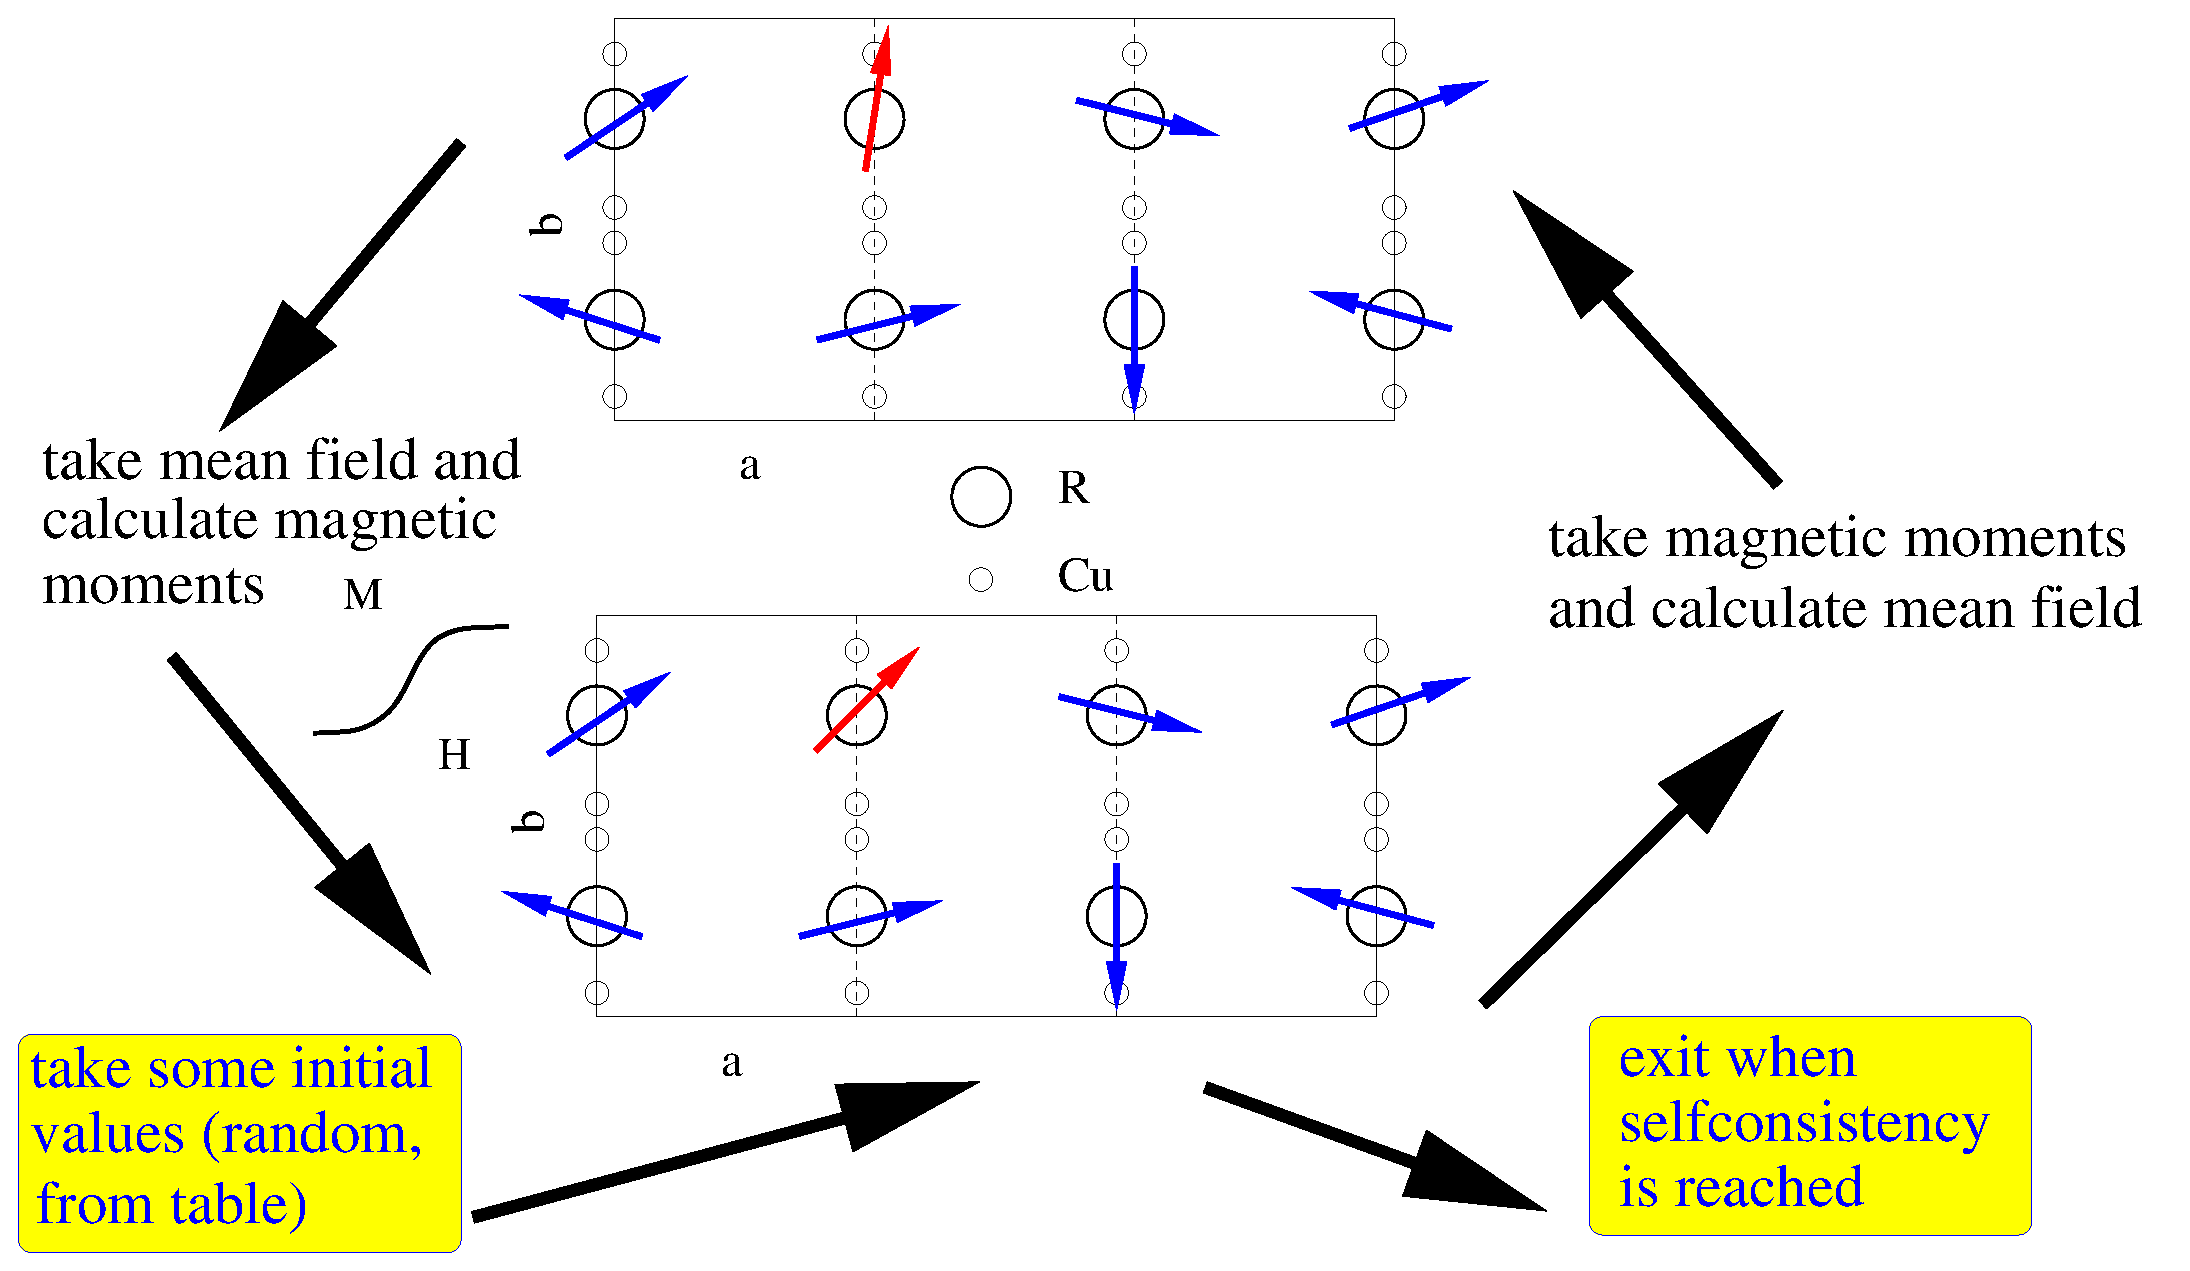
\includegraphics[angle=0,width=0.9\columnwidth]{figsrc/fecalc.eps}
\caption{\label{fecalc}Mean field process of sub {\prg fecalc}.}
\end{figure}

 
\subsubsection{Example {\prg mcphas.ini\index{mcphas.ini}} file for a simple antiferromagnet}

Here is an example of {\prg mcphas.ini\index{mcphas.ini}}, the comments describe the meaning of the different
parameters:

\input{mcphas.ini}



\subsubsection{{\prg mcphas.j\index{mcphas.j}} - lattice and exchange parameters}\label{mcphasj}
This file provides the information about 
the crystallographic
 structure and the magnetic exchange interactions.
For every atom in the crystallographic basis there
has to be given the coordinates, the number of neighbours to be considered, the 
Land\'e factor $g_J$, the single ion property filename and  a set of exchange parameters.
If the exchange parameters (and neighbour positions) are not known for your system, you 
can use the program module {\prg makenn\index{makenn}} (see section \ref{addprog}) to generate 
a list of nearest neighbours and
exchange parameters, currently implemented in {\prg makenn\index{makenn}} are dipolar interactions,
exchange interactions via the Bethe-Slater curve or the RKKY model. Note that in order
to use {\prg makenn\index{makenn}} you have to set up a working {\prg mcphas.j\index{mcphas.j}} file, which may or
may not contain neighbours and interactions.

Use program {\prg addj\index{addj}} to add exchange parameter set stored in different 
such {\prg .j} files (see section~\ref{addprog}).



\begin{description}
\item [Line 1,2:] Comment Lines
\item [Line 3:] lattice constants a,b,c and crystal angles alpha, beta, gamma 
\item [Line 4-6:] primitive lattice vectors
\item [Line 7:] Number of atoms in the primitive crystallographic unit cell ({\prg nofatoms})
\item [Line 8:] a comment line with stars
\item [Line 9:] coordinates  ($d_a$,$d_b$,$d_c$) of 1$^{st}$ magnetic ion in the crystallographic unit cell  with
respect to the lattice vectors $\vec a$,$\vec b$,$\vec c$. The number of neighbours of this 
ion, for which interaction constants are given in the interaction table (nofneighbours). 
If {\prg diagonalexchange}
is set to 0 the 9 components of the exchange tensor are given in column 4-12. 
If {\prg diagonalexchange}
 is 1, only 3 components are given (column 4-6).
If {\prg diagonalexchange}
 is 2, specific components of the exchange tensor can be given in columns 4 onwards. The indices of these components
 must be given in the following line (Line 9a below).
The Land\'e factor of the ion (gJ) and the file name of the corresponding single ion
parameter file (cffilename).
\item [Line 9a:]  If {\prg diagonalexchange=2}, then this line gives the indices of the exchange tensor corresponding to 
 the columns 4 onwards. It must have a variable called {\prg indexexchange} followed by a list of names of components of the interaction
 tensor separated by space. E.g.
 \verb|  #! indexexchange= JaJb JbJc  | 
means column 4 gives the the interaction constant between the
 first angular momentum component of the current ion with the second angular momentum component of its neighbour, whilst 
 column 5 has the interaction constant between the second angular momentum component of this ion with the third component of its
 neighbour. Alternatively, pairs of numbers may be given, as in \verb|  #! indexexchange= 1,2 2,3  |
 Additionally another parameter {\prg symmetricexchange} can be set to 1, where the value in each column is also used 
 for the transposed tensor component. Thus \verb|  #! symmetricexchange=1 indexexchange= JaJb  | is the same as \\
 \verb|  #! indexexchange= JaJb JbJa  | where the 4th and 5th column are the same.
\item [Line 10:]  Comment line
\item [Line 11-(10+nofneighbours):] Interaction table for ion number 1.   
Note: the neighbour coordinates (column 1-3) are given with respect to the lattice vectors
$\vec a$,$\vec b$,$\vec c$. The program then calculates from these values the coordinates
with respect to the primitive lattice $\vec r_1$,~$\vec r_2$,~$\vec r_3$.
($ d_a \vec a + d_b \vec b + d_c \vec c = d_1 \vec r_1 + d_2 \vec r_2 + d_3 \vec r_3$).
Column 4,5,6 \dots contain the components of the interaction tensor $\stackrel{=}{\mathcal J}$. 
Note that in case of non-orthogonal axes the 
components of the moments and the interaction tensor $Ja, Jb, Jc, Jaa, Jbb, Jcc, Jab ...$ 
refer to the orthogonal coordinate system
defined with respect to the nonorthogonal lattice $\vec a,\vec b,\vec c$ as
$Jb||\vec b$, $Jc||(\vec a \times \vec b)$ and $Ja$ perpendicular to $Jb$ and $Jc$.
\item [Line (11+nofneighbours) - end:] for each ion in the unit cell line 8 - (10+nofneighbours)
are repeated.
\end{description}


\vspace{0.5cm}

{\small {\bf Information for experienced users:}
\begin{description}
\item[\prg mcphas.jjj:]
format of exchange parameter file, which only needs a reduced set of exchange
parameters in the input file. Using the program {\prg jjj2j} the file can be transformed
to {\prg mcphas.j\index{mcphas.j}} by adding lines for all the equivalent neighbours. The format definition
of {\prg mcphas.jjj} is the same as {\prg mcphas.j\index{mcphas.j}}, however each line denotes several
equivalent neighbour atoms (instead of only one in {\prg mcphas.j\index{mcphas.j}}) according to the
 following rules:
\begin{itemize}
\item If a nonzero coordinate $d_a$ (or $d_b$,$d_c$) in the interaction table
 corresponds to it's value at the nearest
 lattice point of the primitive lattice,
  additional interactions of the same size
with  neighbours with coordinate $-d_a$ (or $-d_b$,$-d_c$, respectively)
are taken into account. This
holds for each of the three coordinates $d_a$,$d_b$ and $d_c$
 resulting in a maximum
number of 8 equivalent neighbours per line in the interaction table.
\item If the value of $d_a$ (or $d_b$,$d_c$) is zero or differs
from it's value at the nearest lattice point of the primitive lattice, it is 
changed to the value at the nearest lattice point and {\bf no} interaction 
with  neighbours with coordinates $-d_a$ (or $-d_b$,$-d_c$) is
 taken into account. If such
 interaction is needed it may be given in a different line and may
have different magnitude. In this way also crystallographic lattices
with no mirror symmetry may be described.
\end{itemize}
\item[\prg mcphas.coq:]   exchange parameters etc [ in old format]...see examples for details, use {\prg coq2jjj} to 
transform {\prg mcphas.coq} to {\prg mcphas.jjj} format
\end{description}

}


\subsubsection{Example {\prg mcphas.j\index{mcphas.j}} file for a simple antiferromagnet}

Here are example files of a tetragonal antiferromagnet with nearest neighbour interactions, all
files are equivalent:

{\small
\begin{verbatim} 
# simple antiferromagnet 
#<!--mcphase.mcphas.j-->
#***************************************************************
# Lattice Constants (A)
#! a=4.3843 b=4.3843 c=2.4194 alpha=  90 beta=  90 gamma=  90
#! r1a=   1 r2a=   0 r3a=   0
#! r1b=   0 r2b=   1 r3b=   0   primitive lattice vectors [a][b][c]
#! r1c=   0 r2c=   0 r3c=   1
#! nofatoms=1  nofcomponents=3  number of atoms in primitive unit cell/number of components of each spin
# ****************************************************************************
#! da=  0 [a] db=  0 [b] dc=  0 nofneighbours=2 diagonalexchange=0 gJ=0.857143 cffilename=Ce3p.sipf
# da[a] db[b] dc[c] Jaa[meV] Jbb[meV] Jcc[meV] Jab[meV] Jba[meV] Jac[meV] Jca[meV] Jbc[meV] Jcb[meV]
+0	+0	+1	-0.1	-0.1	-0.1   0  0  0  0  0  0
+0	+0	-1	-0.1	-0.1	-0.1   0  0  0  0  0  0
#\end{verbatim}
}

Using diagonalexchange this may be shortened to

{\small
\begin{verbatim} 
# simple antiferromagnet 
#<!--mcphase.mcphas.j-->
#***************************************************************
# Lattice Constants (A)
#! a=4.3843 b=4.3843 c=2.4194 alpha=  90 beta=  90 gamma=  90
#! r1a=   1 r2a=   0 r3a=   0
#! r1b=   0 r2b=   1 r3b=   0   primitive lattice vectors [a][b][c]
#! r1c=   0 r2c=   0 r3c=   1
#! nofatoms=1  nofcomponents=3  number of atoms in primitive unit cell/number of components of each spin
# ****************************************************************************
#! da=  0 [a] db=  0 [b] dc=  0 nofneighbours=2 diagonalexchange=1 gJ=0.857143 cffilename=Ce3p.sipf
# da[a] db[b] dc[c] Jaa[meV] Jbb[meV] Jcc[meV] Jab[meV] Jba[meV] Jac[meV] Jca[meV] Jbc[meV] Jcb[meV]
+0	+0	+1	-0.1	-0.1	-0.1   
+0	+0	-1	-0.1	-0.1	-0.1   
#\end{verbatim}
}

with indexexchange option the sequence of two ion interaction parameters can be changed and
zero parameters may be omitted:

{\small
\begin{verbatim} 
# simple antiferromagnet 
#<!--mcphase.mcphas.j-->
#***************************************************************
# Lattice Constants (A)
#! a=4.3843 b=4.3843 c=2.4194 alpha=  90 beta=  90 gamma=  90
#! r1a=   1 r2a=   0 r3a=   0
#! r1b=   0 r2b=   1 r3b=   0   primitive lattice vectors [a][b][c]
#! r1c=   0 r2c=   0 r3c=   1
#! nofatoms=1  nofcomponents=3  number of atoms in primitive unit cell/number of components of each spin
# ****************************************************************************
#! da=  0 [a] db=  0 [b] dc=  0 nofneighbours=2 diagonalexchange=2 gJ=0.857143 cffilename=Ce3p.sipf
# da[a] db[b] dc[c] Jaa[meV] Jbb[meV] Jcc[meV] Jab[meV] Jba[meV] Jac[meV] Jca[meV] Jbc[meV] Jcb[meV]
#! indexexchange = JaJa JaJc JcJa JbJb JcJc
+0	+0	+1	-0.1 0 0 -0.1	-0.1  
+0	+0	-1	-0.1 0 0 -0.1	-0.1  
#\end{verbatim}
}

{\small
\begin{verbatim} 
# simple antiferromagnet 
#<!--mcphase.mcphas.j-->
#***************************************************************
# Lattice Constants (A)
#! a=4.3843 b=4.3843 c=2.4194 alpha=  90 beta=  90 gamma=  90
#! r1a=   1 r2a=   0 r3a=   0
#! r1b=   0 r2b=   1 r3b=   0   primitive lattice vectors [a][b][c]
#! r1c=   0 r2c=   0 r3c=   1
#! nofatoms=1  nofcomponents=3  number of atoms in primitive unit cell/number of components of each spin
# ****************************************************************************
#! da=  0 [a] db=  0 [b] dc=  0 nofneighbours=2 diagonalexchange=2 gJ=0.857143 cffilename=Ce3p.sipf
# da[a] db[b] dc[c] Jaa[meV] Jbb[meV] Jcc[meV] Jab[meV] Jba[meV] Jac[meV] Jca[meV] Jbc[meV] Jcb[meV]
#! indexexchange = 1,1 1,3, 3,1 2,2 3,3
+0	+0	+1	-0.1 0 0 -0.1	-0.1  
+0	+0	-1	-0.1 0 0 -0.1	-0.1  
#\end{verbatim}
}


using symmetricexchange together with indexexchange will assume that the interaction tensor is symmetic and 
only half of it may be given:

{\small
\begin{verbatim} 
# simple antiferromagnet 
#<!--mcphase.mcphas.j-->
#***************************************************************
# Lattice Constants (A)
#! a=4.3843 b=4.3843 c=2.4194 alpha=  90 beta=  90 gamma=  90
#! r1a=   1 r2a=   0 r3a=   0
#! r1b=   0 r2b=   1 r3b=   0   primitive lattice vectors [a][b][c]
#! r1c=   0 r2c=   0 r3c=   1
#! nofatoms=1  nofcomponents=3  number of atoms in primitive unit cell/number of components of each spin
# ****************************************************************************
#! da=  0 [a] db=  0 [b] dc=  0 nofneighbours=2 diagonalexchange=2 gJ=0.857143 cffilename=Ce3p.sipf
# da[a] db[b] dc[c] Jaa[meV] Jbb[meV] Jcc[meV] Jab[meV] Jba[meV] Jac[meV] Jca[meV] Jbc[meV] Jcb[meV]
#! symmetricexchange=1 indexexchange = JaJa JaJc JbJb JcJc
+0	+0	+1	-0.1 0  -0.1	-0.1  
+0	+0	-1	-0.1 0  -0.1	-0.1  
#\end{verbatim}
}


\subsubsection{Single Ion Property Input Files}\label{sifile}

In order to speed up calculations or treat special problems a large 
variety of single ion modules is available. This includes the
option to load a user written single ion module. Details are 
given in chapter~\ref{simod}.

The first time user of {\prg McPhase} should use the module {\prg so1ion}\index{so1ion} and 
create an appropriate single ion property input file as described in
section \ref{cf1ion}. A good starting point are several examples
given in directory {\prg examples}.


\subsubsection{Example single ion property file  for a simple antiferromagnet}

Here is an example file {\prg mcphas.cf1} describing the anisotropy of a 
simple antiferromagnet with Ce atoms having basal plane anisotropy. Note the
axis convention xyz$||$abc, in case of non-orthogonal axes the convention 
is $y||\vec b$, $z||(\vec a \times \vec b)$ and $x$ perpendicular to $y$ and $z$.


\input{mcphas.cf1}

\subsubsection{{\prg mcphas.tst\index{mcphas.tst}} - input file of test spin-configurations (optional)}
This file is optional and contains
some test momentum configurations to be used for the calculation
             of the free energy. Mind that
\begin{itemize}
\item  in the file header the number of atoms in the primitive
       crystallographic unit cell and the number of components
       of the spin vector have to be given.
\item  at the end of the
 file there must be no empty lines !
\end{itemize}

The momentum - configurations tables always refer to spins sitting on
the primitive lattice ${\mbf r}_i$. If more than one atom is in
the primitive basis, the momentum gets $3n$ components ($n=$ number
of atoms in the crystallographic basis). See {\prg ./examples/ndcu2b\_new/} for
examples of a two atom basis. Units of these tables are that of total 
angular momentum $<J>$.

\subsubsection{Example {\prg mcphas.tst\index{mcphas.tst}} file  for a simple antiferromagnet}

Here is the file {\prg mcphas.tst\index{mcphas.tst}} for the simple antiferromagnet example
describing some spin configurations
to be used as starting values for the mean field process:

\input{mcphas.tst}
Note, in case of non-orthogonal axes the convention 
is $mb||\vec b$, $mc||(\vec a \times \vec b)$ and $ma$ perpendicular to $mb$ and $mc$.

\subsubsection{subdirectory {\prg ./results} - directory where calculated data is stored}

In order to be able to save the results of a calculation the directory {\prg ./results} has to
exist. Mind that all files in this directory will be overwritten without warning. 

\subsubsection{subdirectory {\prg ./fit} - experimental data for fit (optional) } 

In order that {\prg McPhase} can calculate the standard deviation between
 experimental data and the results of the simulation, some experimental data
 can be given in the subdirectory {\prg ./fit}. The filenames and the data-format
 are the same as the output files of {\prg McPhas}, e.g. {\prg mcphas.fum}, {\prg mcphas.hkl}
 etc. {\prg McPhase} looks into the directory {\prg ./fit} and if it finds any
 of these files, the standard deviation is increased correspondingly. 

What measurement data can be used to calculate a standard deviation ?

\begin{description}
\item[{\prg mcphas.fum}] if given in column 11, 12, 13 in {\prg ./fit/mcphas.fum} the
            magnetisation in the $a$, $b$ and $c$ direction is used for calculation
	    of the standard deviation sta. The standard deviation is calculated
	    as ${\rm sta}=\sum_{\rm data points i} ({\mbf m}_i^{calc}-{\mbf m}_i^{meas})^2$.
	    All three components of the magnetic moment have to be given and are used.

\end{description}

Note that the measured data has to be given in those (H-T) points which are 
calculated by mcphas\index{mcphas} in order to be used by the program to increase {\prg sta}.
It is usually most effective to fit only few data points, because a large set
of data points will not improve the quality of the fit and only require a large
amount of calculation time.



\subsection{Starting a simulation}
\label{start}

To start the simulation goto the directory containing the
input files {\prg mcphas.ini, mcphas.j, etc. } and type

\begin{description}
\item[\prg mcphas] to run the program generating stepwise $H-T$ values 
              in a loop given by {\prg mcphas.ini\index{mcphas.ini}} (you can also press the
              symbol in the {\prg McPhase - Explorer} window).
\item[\prg mcphas\index{mcphas} [file]]  to run the program with an input file --   
             {\prg file} contains T ha hb hc values to be calculated 
             if [file] is not given, xmin xmax xstep (xT xHa xHb xHc)
             ymin ymax ystep (yT yHa yHb yHc) is read from file {\prg mcphas.ini\index{mcphas.ini}}
	     and phase diagram is calculated
\item[\prg mcphas\index{mcphas} -h]  to  print help and version of {\prg McPhas}.
\item[\prg mcphas\index{mcphas} -stamax 14]  end mcphas\index{mcphas} if standard deviation exceeds 14.
\item[\prg mcphas\index{mcphas} -a] avoid overwriting output files in results, append new results to existing files
\item[\prg mcphas\index{mcphas} -v]  to  enable verbose mode with lots of messages of {\prg McPhas}. Specifically
the verbose mode enables the following features:
  \begin{itemize}
			          \item more information is printed out, 
			          \item the q-vectors file {\prg ./results/mcphas.qvc} will contain 
				    the explicit spin configurations
			          \item the display\index{display} on screen (ghostview window using 
				     {\prg ./results/.sps.eps}) will be updated not only 
				    when a H-T point has been finished but always 
				    when a structure with smaller free energy 
				    has been stabilised
  \end{itemize}
\item[\prg mcphasit\index{mcphas}] to start mcphase in commandline mode without opening any window
\end{description}

\vspace{1cm}
{\em Exercises:}
\begin{itemize}
\item Look at the input files for {\prg McPhase} given in the directory
{\prg examples/ndcu2b\_new}.  How many atoms are contained in the crystallographic basis ?
\item
Start the simulation by typing the command {\prg mcphas}.
\end{itemize}



\subsection{Options for a running simulation}
... when the program is running, the options in the main window
can be changed. Pressing ''displayall'' displays the current spin-configuration
at each iteration step. Pressing ''log fe vs Q'' appends free energy vs Q
data to {\prg mcphas.log} for every ($T-H$) point.


The file {\prg ./results/.spins.eps} is used to show the information about the currently calculated
spin structure on the screen using the postscript file viewer ghostview.

The file {\prg ./results/.mcphas.fum} contains the information of the magnetisation curve
which is currently calculated. This information is automatically displayed on the screen.


The program {\prg display} (see section \ref{display}) can be used 
for the online display\index{display} of any other
curve(s).


\subsection{Output Files - {\prg mcphas.qvc,phs,sps,mf,fum,j1...,xyt,hkl} }\label{outputfiles}
 (in directory ./results/ after a simulation run) 

\begin{figure}[htb]%h=here, t=top, b=bottom, p=separate figure page
\begin{center}\leavevmode
\includegraphics[angle=0, width=0.3\textwidth]{figsrc/magnetization_ndcu2.ps}
\end{center}
\caption{Calculated magnetisation of NdCu$_2$ for field parallel to the orthorhombic $b$-direction.}
\label{magnetization}
\end{figure}

\begin{figure}[htb]%h=here, t=top, b=bottom, p=separate figure page
\begin{center}\leavevmode
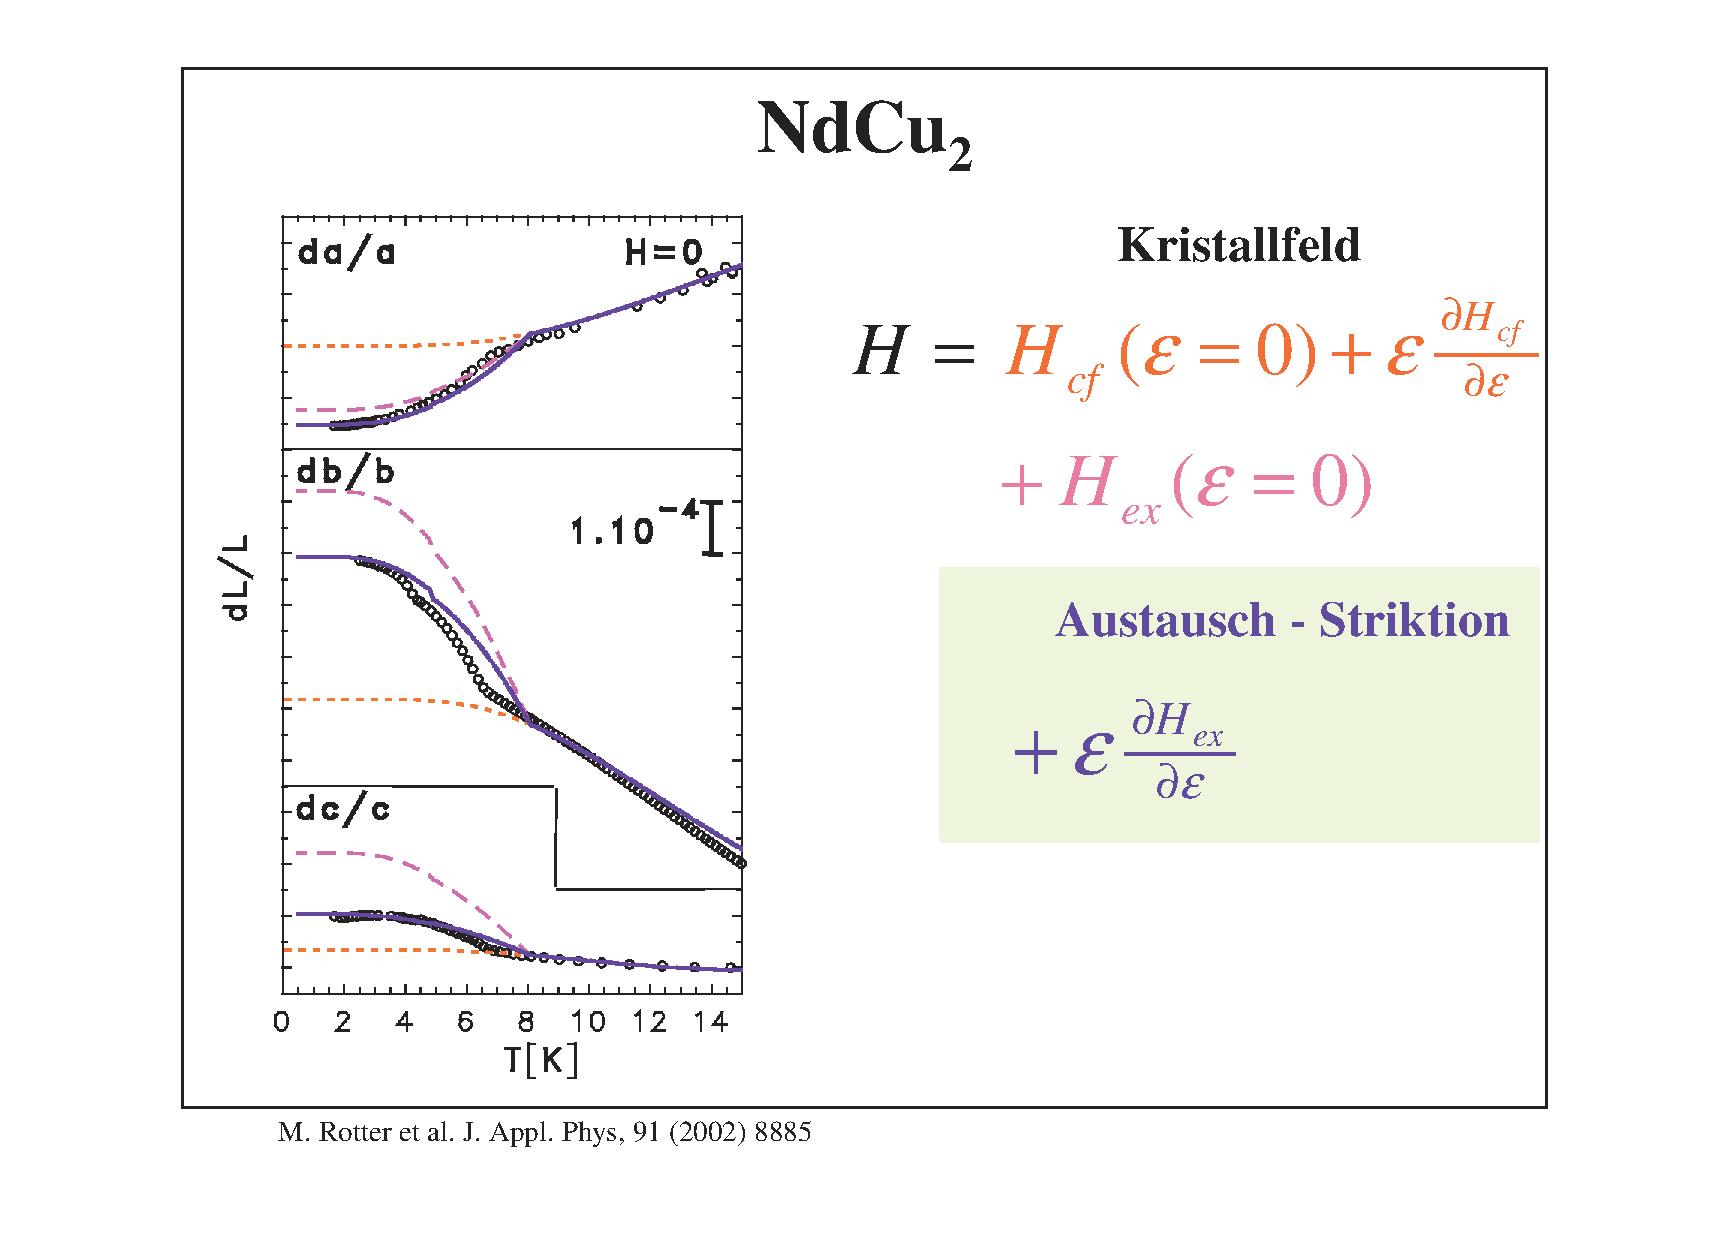
\includegraphics[angle=0, width=0.8\textwidth]{figsrc/magnetostriction_ndcu2.eps}
\end{center}
\caption{Calculated spontaneous magnetostriction of NdCu$_2$.}
\label{magnetostrictiongraphic}
\end{figure}

\begin{description}
\item [\prg mcphas.qvc]    the set of test q-vectors used for calculation of free energy.
                           Components of these q vectors refer to the reciprocal lattice $\vec a^*,\vec b^*,\vec c^*$.
\item [\prg mcphas.phs]    spin-configuration table of different types of spin-configurations. 
                            Note, in case of non-orthogonal axes the convention in these tables 
                            is $mb||\vec b$, $mc||(\vec a \times \vec b)$ and $ma$ perpendicular to $mb$ and $mc$.

                           {\em Note}: 
                           there is no natural criteria for deciding, if one spin-configuration is
			   different from another one. Therefore the list of ''different''
			   spin-configurations is dependent on the meaning of ''different''.
			   
			   The program {\prg McPhase} decides whether a spin-configuration is
			   different from another by a simple criteria, namely by the
			   angle between the spins. Comparing two spin configurations it calculates
			   the angle between corresponding spins and if for one spin the
			   angle is not small, the configuration is treated as a different
			   configuration. Therefore for example a ferromagnet with moments
			   in $a$ has a different spin configuration than a ferromagnet with
			   moments in $b$ direction. 
\item [\prg mcphas.sps]    $T-H$ dependence of spin-configuration. The spin configurations stored in this
                           file may be displayed using the program {\prg spins\index{spins}}, an example is given
			   in figure~\ref{spingraphic}.
                            Note, in case of non-orthogonal axes the convention for applied field $Ha, Hb,Hc$ and
                            also for the moment components $ma, mb, mc$ in these tables 
                            is $mb||\vec b$, $mc||(\vec a \times \vec b)$ and $ma$ perpendicular to $mb$ and $mc$.

\item [\prg mcphas.mf]     $T-H$ dependence of exchange field configuration, stored as $g_J \mu_B H_{xc}(i)$(unit is in meV)
                            for i=1,2,...,number of spins in magnetic unit cell.
                            Note, in case of non-orthogonal axes the convention for applied field $Ha, Hb,Hc$ and
                            also for the mean field components in these tables 
                            is $Hb||\vec b$, $Hc||(\vec a \times \vec b)$ and $Ha$ perpendicular to $Hb$ and $Hc$.
\item [\prg mcphas.fum]    free energy, magnetic energy (the derivative with respect to temperature gives the specific %%@
heat),
                           magnetisation data and (if cfield is used with higher order interactions)
                           expectation values of the Stevens Operators $<O_l^m>$ . As an example for the information
			   contained in this file the calculated magnetisation and magnetostriction of NdCu$_2$ is shown in
			   figures~\ref{magnetization} and ~\ref{magnetizationgraphic}.
                            Note, in case of non-orthogonal axes the convention for applied field $Ha, Hb,Hc$ and
                            also for the magnetisation components $ma,mb,mc$ in these tables 
                            is $Hb||\vec b$, $Hc||(\vec a \times \vec b)$ and $Ha$ perpendicular to $Hb$ and $Hc$.

\item [\prg mcphas1.j1 .j1 .j2 ...] 
               spin-spin correlation functions for sub-lattice 1 neighbour 1 2 ...
	       (linear combination is proportional to magnetostriction)
	       The spin-spin correlation functions for neighbour $k$ are defined by
	       the following sum of dyadic products:

	       \begin{equation}
	        \frac{1}{n}\sum_{s=1}^n <{\mbf J}^s> \times  <{\mbf J}^{s+k}>
	       \end{equation}
	       with $n$ being the number of moments in the magnetic unit cell.
	       Single ion and two-ion magnetostriction can be calculated using the $<O_l^m>$ and the
	       spin-spin correlation functions. As an example the magnetostriction analysis of
	       NdCu$_2$ is shown in figure~\ref{magnetostrictiongraphic}. For details 
             please refer to~\cite{rotter02-8885}.
                            Note, in case of non-orthogonal axes the convention for applied field $Ha, Hb,Hc$ and
                            also for the moment components in these tables 
                            is $Hb||\vec b$, $Hc||(\vec a \times \vec b)$ and $Ha$ perpendicular to $Hb$ and $Hc$.
\item [\prg mcphas.xyt]    phase diagram as x,y,T, H, phase-number j according to spin-configuration table
               given in mcphas.phs, a periodicity key, nettomoments <J>.
 Figure~\ref{phasediagramgraphic}
	       shows the phase diagram of NdCu$_2$ for magnetic fields parallel to the orthorhombic $b$-direction.
                            Note, in case of non-orthogonal axes the convention for applied field $Ha, Hb,Hc$ 
                             in these tables 
                            is $Hb||\vec b$, $Hc||(\vec a \times \vec b)$ and $Ha$ perpendicular to $Hb$ and $Hc$.
\item [\prg mcphas.hkl]    calculated (unpolarised) neutron diffraction data (the calculated magnetic intensities
    correspond to the magnetic structure + Polarisation factor. The
    Lorentz-factor , magnetic form factor and  instrumental corrections are not calculated.)
 As an example figure~\ref{neutintgraphic}
    shows the calculated temperature dependence of magnetic amplitudes for NdCu$_2$.
                           $h,k,l$ refer to the reciprocal lattice $\vec a^*,\vec b^*,\vec c^*$.
                            Note, in case of non-orthogonal axes the convention for applied field $Ha, Hb,Hc$ 
                             in these tables 
                            is $Hb||\vec b$, $Hc||(\vec a \times \vec b)$ and $Ha$ perpendicular to $Hb$ and $Hc$.
    
\item [\prg mcphasa.hkl]    Fourier Transform of the $a$-component of the magnetic Moments.
                           $h,k,l$ refer to the reciprocal lattice $\vec a^*,\vec b^*,\vec c^*$.
                            Note, in case of non-orthogonal axes the convention for applied field $Ha, Hb,Hc$ and
                            the magnetic moment component in these tables 
                            is $Hb||\vec b$, $Hc||(\vec a \times \vec b)$ and $Ha$ perpendicular to $Hb$ and $Hc$.
\item [\prg mcphasb.hkl]    Fourier Transform of the $b$-component of the magnetic Moments.
                           $h,k,l$ refer to the reciprocal lattice $\vec a^*,\vec b^*,\vec c^*$.
                            Note, in case of non-orthogonal axes the convention for applied field $Ha, Hb,Hc$ and
                            the magnetic moment component in these tables 
                            is $Hb||\vec b$, $Hc||(\vec a \times \vec b)$ and $Ha$ perpendicular to $Hb$ and $Hc$.
\item [\prg mcphasc.hkl]    Fourier Transform of the $c$-component of the magnetic Moments.
                           $h,k,l$ refer to the reciprocal lattice $\vec a^*,\vec b^*,\vec c^*$.
                            Note, in case of non-orthogonal axes the convention for applied field $Ha, Hb,Hc$ and
                            the magnetic moment component in these tables 
                            is $Hb||\vec b$, $Hc||(\vec a \times \vec b)$ and $Ha$ perpendicular to $Hb$ and $Hc$.
\end{description} 

\vspace{1cm}
{\em Exercises:}
\begin{itemize}
\item Look at the output files of {\prg McPhase}  in the directory
{\prg examples/ndcu2b\_new/results}.  At which magnetic field
the ferromagnetically aligned state is achieved (at $T=$2~K)?
\item
What is the propagation vector in the different antiferromagnetic phases at $T=$2~K ?
\end{itemize}



\subsubsection{{\prg mcphas.tst\index{mcphas.tst}} - input file of test spin-configurations (optional)}
This file is optional and contains
some test momentum configurations to be used for the calculation
             of the free energy. Mind that
\begin{itemize}
\item  in the file header the number of atoms in the primitive
       crystallographic unit cell and the number of components
       of the spin vector have to be given.
\item  at the end of the
 file there must be no empty lines !
\end{itemize}

The momentum - configurations tables always refer to spins sitting on
the primitive lattice ${\mbf r}_i$. If more than one atom is in
the primitive basis, the momentum gets $3n$ components ($n=$ number
of atoms in the crystallographic basis). See {\prg ./examples/ndcu2b\_new/} for
examples of a two atom basis. Units of these tables are that of total 
angular momentum $<J>$.

\subsubsection{Example {\prg mcphas.tst\index{mcphas.tst}} file  for a simple antiferromagnet}

Here is the file {\prg mcphas.tst\index{mcphas.tst}} for the simple antiferromagnet example
describing some spin configurations
to be used as starting values for the mean field process:

\section{{\prg mcphas} - calculation of thermodynamic properties (Magnetisation, Susceptibility, Specific Heat, Neutron %%@
Diffraction, etc.)}
\label{runmcphas}

In order to perform calculations beyond the capabilities of {\prg cfield\index{cfield}} it is necessary
to use the program {\prg mcphas}. 
\begin{itemize}
\item As a first step it is possible to
calculate the thermodynamic properties such as magnetisation or specific heat
considering only single ion effects. In this case all the exchange parameters
have to be set to zero in {\prg mcphas.j\index{mcphas.j}}. 
\item for more advanced calculations the two - ion interactions have to be
considered and may lead to magnetic order. {\prg mcphas} can perform 
calculations in the ordered state in the following way: for 
a given temperature $T$ and magnetic field $\mbf H$ (vector)
several possible magnetic structures are stabilised
by a mean field algorithm and the free energy is 
calculated. The initial values for this mean-field procedure are
modified by a Monte Carlo process.


The temperature and magnetic field is varied during the calculation
and thereby it is possible to map out the magnetic phase diagram.
\end{itemize}

The program produces a plot of the stabilised magnetic
structures and the magnetisation on screen, the
output files contain additional information 
such as calculated magnetoelastic and  neutron-scattering
data. Several graphic programs easy the visualisation of the
calculated data (section~\ref{graphics}).



\subsection{Input Files}
The program {\prg McPhase} needs the following input files (all in the same directory)
 in order to run:

\begin{enumerate}
\item {\prg mcphas.ini\index{mcphas.ini}}
 - controlling the algorithm
\item {\prg mcphas.j\index{mcphas.j}}
  - lattice and exchange parameters
\item {\prg mcphas.tst\index{mcphas.tst}(optional)}  - test spin configurations
\item {\prg single-ion property files}
\item {\prg directory ./results/}
 - directory where calculated data is stored
\item {\prg directory ./fit} - experimental data for fit (optional)
\end{enumerate}


 All
 of these input files have to be in one directory and the program
has to be started in this directory. The results of the simulation
are then stored in the  subdirectory ./results/, which must exist before starting
the program 
... see directory ./examples/ for some examples.
 In order to prepare these files
for a new calculation it is best to take them from an example, copy the files
to a new directory and make the
modifications  to adapt them to the new problem.

\subsubsection{Example - a simple antiferromagnet}

In the following description of the input files we will always refer
to a simple example: a simple antiferromagnet
on a primitive orthorhombic lattice. The first time user
will thus have a simple example to follow, all corresponding
files are given in the directory {\prg tutorial/03magnetic\_phases\_mcphas/simpleAF}.
 

\subsubsection{{\prg mcphas.ini\index{mcphas.ini}} - controlling the algorithm}
   Initial file containing algorithm control parameters, for instance the range and spacing of
   propagation vectors Q or the number of Monte Carlo trials for initial spin configurations
    - {\em mind}: this
   file is rewritten and reread  when running the program and may be changed by the
   user in order to manipulate the running simulation.

{\prg mcphas.ini\index{mcphas.ini}} consists of several sections:
\begin{description}
\item [MCPHASE RUNTIME CONTROL:] this section contains the parameters
controlling the status of the calculation.
\item [XY PHASEDIAGRAM PARAMETERS:] here the temperature and field range and
step widths of the calculation are specified.
The definition of the x and y
axis in terms of temperature and magnetic field is followed by the
corresponding range and step width. An offset may be given for all
field and temperature values.
Note that for most cases of interest
this offset is zero (T0=0, Ha0=0, Hb0=0, Hc0=0).
 For the simple case of calculating a Temperature-Field phase diagram
 It is just necessary to set xT=1 and give the temperature range by
xmin/xmax/xstep. For field in b direction then just set yHb=1 and 
define the range in ymin/ymax/ystep.
In case of non-orthogonal axes the applied magnetic field
components $Ha, Hb, Hc$ refer to the orthogonal coordinate system
defined with respect to the nonorthogonal lattice $\mbf a,\mbf b,\mbf c$ as
$Hb||\mbf b$, $Hc||(\mbf a \times \mbf b)$ and $Ha$ perpendicular to $Hb$ and $Hc$.

\item [GENERATION OF SPINCONFIGURATIONS:] at the beginning of the program
some initial values of spin configurations are generated from a set of 
propagation vectors. This section defines the range of propagation vectors
and the step width.
Depending on the value of the propagation Q with respect to the primitive reciprocal lattice
1-, 2- or 3-dimensional simulations of magnetic lattices
are possible. It is advisable to 
think carefully about the chosen range and spacing of Q vectors in order
to limit calculation time.
 
For example a good starting point is to begin with a calculation with large
step widths (e.g. 0.1)  covering the Brillouin zone. This should give an idea
of the propagation vectors which are stabilised. An advanced calculation
could then fine tune the propagation and determine its accurate value (using
small step widths in a limited area of the zone).
The verbose option of {\prg mcphas} allows to inspect the propagation vectors
which are actually used in the calculation.
Trick: in order to get a quick overview of the
q-vector range covered by the mcphas\index{mcphas} simulation start mcphas, exit and 
just type {\prg felog ./results/mcphas.qvc} (need {\prg perl,perldl,pdl,pgplot} packages).

In order to limit calculation time, the maximum periodicity
of the magnetic unit cell with respect to the crystallographic unit cell 
(maxqperiod) and the maximum number of spins in the magnetic unit cell 
(maxnofspins) can be limited. Also the maximum number of test spin configurations
in the internal table can be limited (maxnoftestspincf).
A critical feature with respect to calculation time is also the number of
spin configurations which are generated by a random process from a tabulated
SPINCONFIGURATIONS during the calculation. 

In summary the variables in this section are mainly important to adapt the
program to a given computer system with finite speed. They have to be set
to optimise between speed and accuracy of the calculation. In order to
find appropriate values it is best to perform some calculations 
and restrict the parameters step by step if insufficient speed is obtained.
Also the examples included in the program package may serve as starting
points.

\item [PARAMETERS FOR SUB FECALC SELFCONSISTENCY PROCESS:] the most important
procedure in the module {\prg mcphas} is the sub fecalc. In this part of the 
program the self consistent calculation of the magnetic moment configuration
is performed as shown schematically in fig.~\ref{fecalc}. 
In the mean field approximation the Hamiltonian~(\ref{hamilton}) is approximated
by

\begin{equation}
 {\mathcal H}=\sum_n H_{SI}^n + E_{corr}
\end{equation}

with the single ion Hamiltonian (in case of module {\prg so1ion\index{so1ion}})

\begin{equation}
H_{SI}^n=  B_l^m O_{lm}({\mbf J}^n) 
	     - g_{Jn} \mu_B {\mbf J}^n {\mbf H^n_{eff}} 
\end{equation}

and the correction term

\begin{equation}
E_{corr}=\frac{1}{2}\sum_{n} g_{Jn} \mu_B \langle {\mbf J}^n
 \rangle (\mbf H^n_{eff}-\mbf H) 
\end{equation}

and with the mean fields $ \mbf H^n_{eff}$ given by

\begin{equation}\label{meanfield}
\mbf H^n_{eff}=\mbf H + \mbf H^n_{xc}=\mbf H+\sum_{{\mbf G'}n'} \frac{{\mathcal J}
(\mbf r_n-(\mbf G'+\mbf r_{n'}))}{g_{Jn}\mu_B } \langle{\mbf
J}^{n'}\rangle
\end{equation}

These mean fields and the moments $\langle \mbf J^n \rangle$ 
are determined in a self consistent
way. For a given magnetic unit cell and initial configuration 
of magnetic moments
the mean fields are calculated according to equation~(\ref{meanfield}). 
Then, for each
magnetic ion the single ion property module is taken 
and the magnetic moment $\langle \mbf J^n \rangle$ is 
calculated from it's mean field. The mean fields are used again in equation~(\ref{meanfield})
and so on .... until convergence is reached. 
Then, the free energy ($f=-kT\sum_n \ln(z_n) + E_{corr}$ ) 
of the stabilised
configuration is calculated (this is why this sub is called {\prg fecalc}). 
The free energies of a lot of different stabilised configurations have to
be compared in order to find out which configuration has lowest free energy, i.e.
is stable in thermal  equilibrium.

It may happen that this process does
not converge due to bad choice of the initial configuration, therefore a maximum number
of mean field loops has to be given by the user.
The results of a calculation may be significantly influenced by
changing parameters such as the maximum number of iteration loops 
in this section. 
In fact the simulation is always a compromise of calculation time and accuracy: if only
a few initial spin configurations are tried at each (H-T) point, the calculation speed is
fast, however it is possible that the program misses the magnetic structure with the
lowest free energy. The same holds if other critical parameters of the simulation are
restricted too much.
 

\item [OUTPUT OF PHYSICAL PROPERTIES:]
Some options for the output of the calculation can be changed in this section.
\end{description}

\begin{figure}[hb]
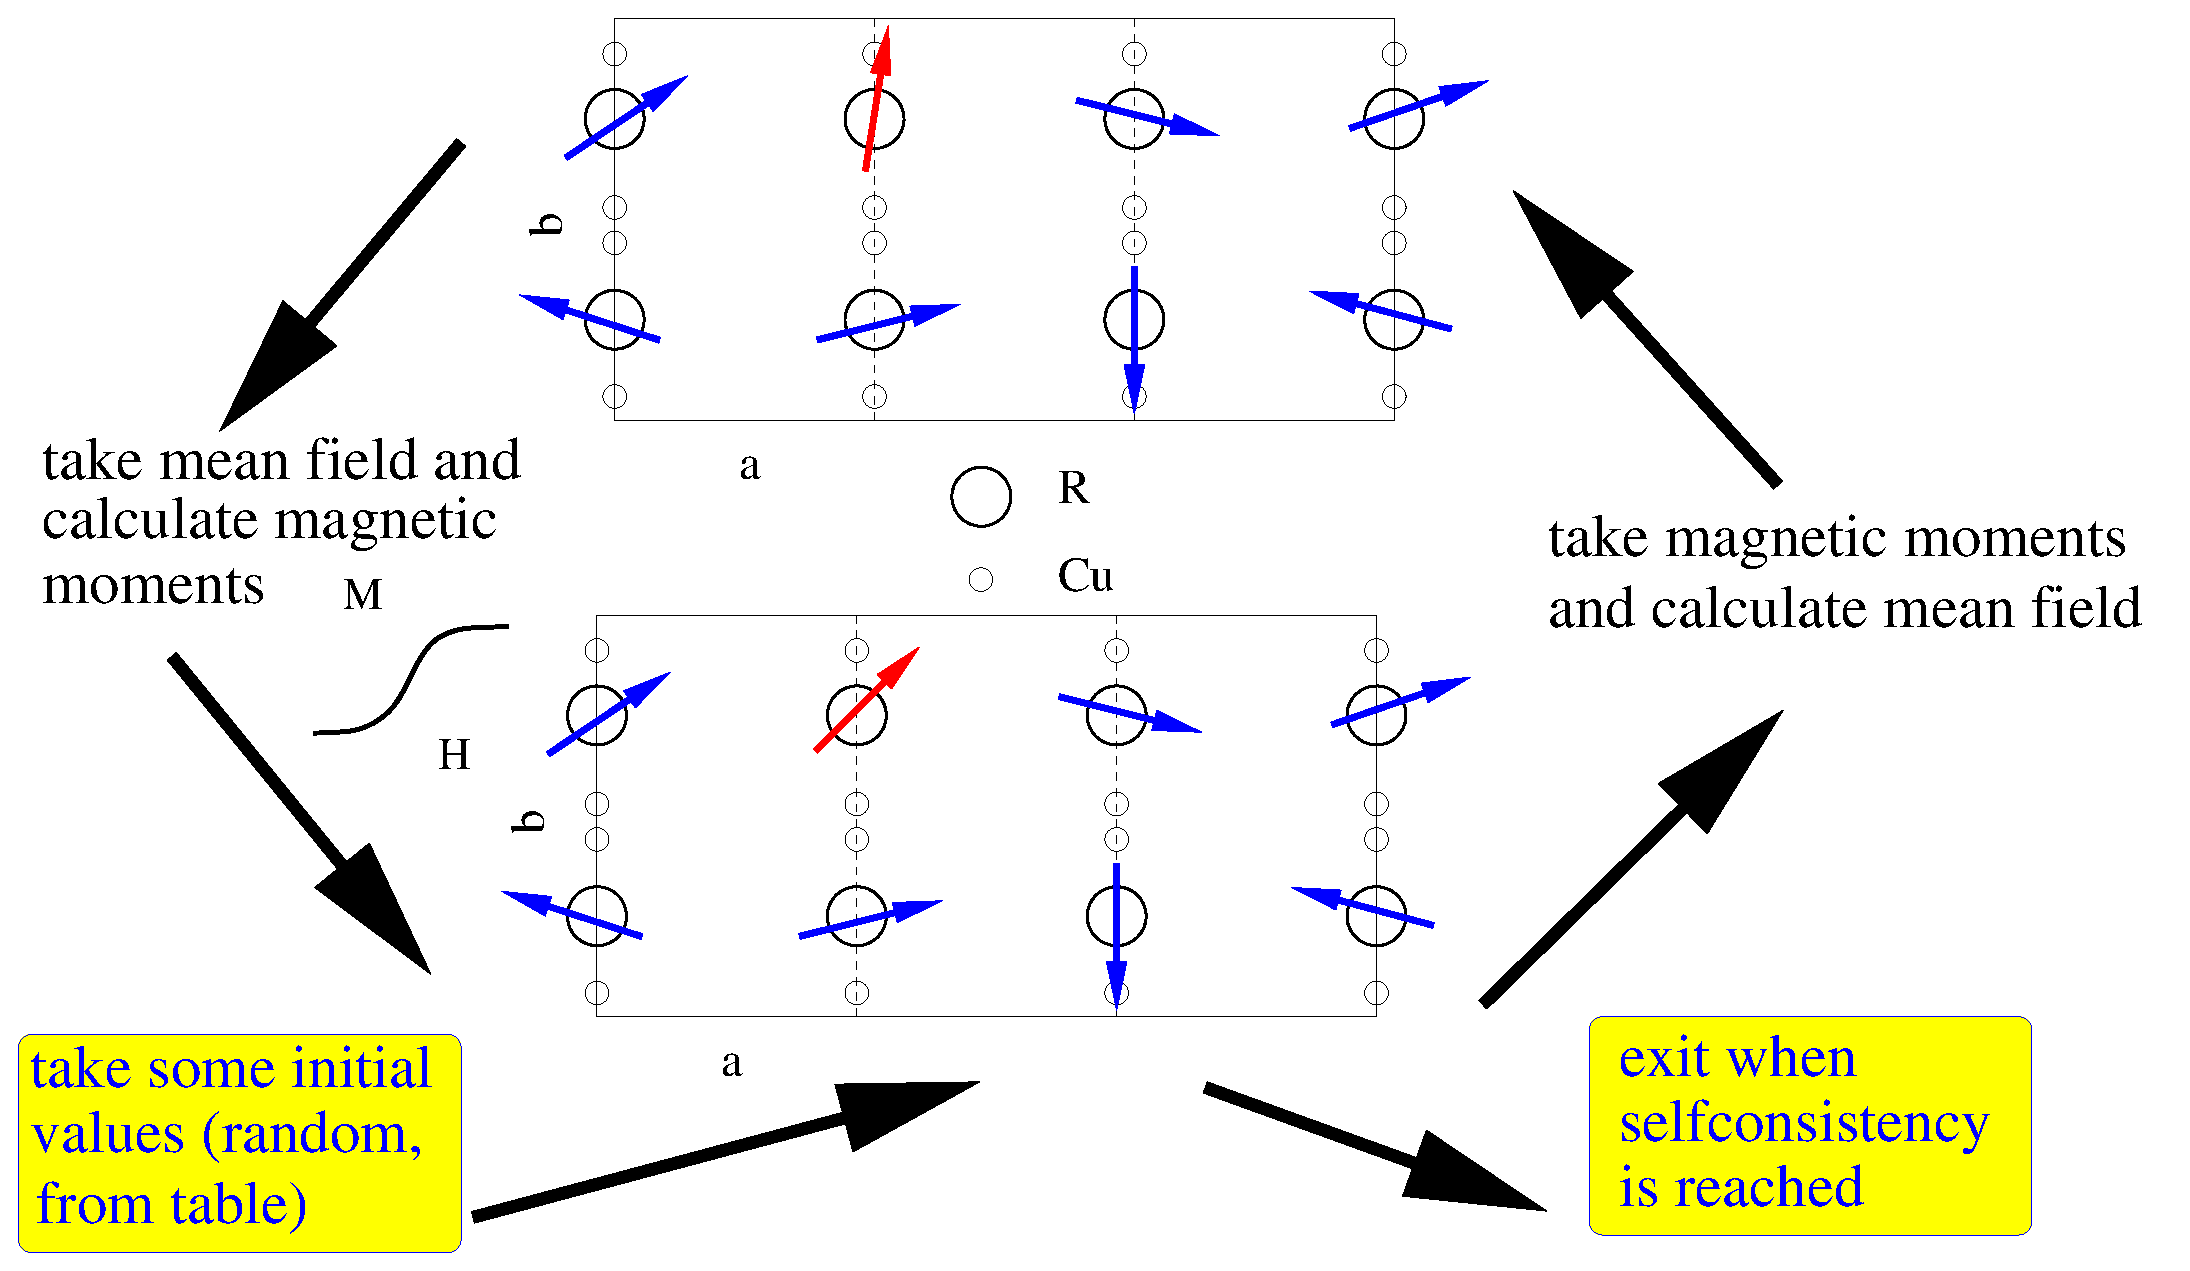
\includegraphics[angle=0,width=0.9\columnwidth]{figsrc/fecalc.eps}
\caption{\label{fecalc}Mean field process of sub {\prg fecalc}.}
\end{figure}

 
\subsubsection{Example {\prg mcphas.ini\index{mcphas.ini}} file for a simple antiferromagnet}

Here is an example of {\prg mcphas.ini\index{mcphas.ini}}, the comments describe the meaning of the different
parameters:

\input{mcphas.ini}



\subsubsection{{\prg mcphas.j\index{mcphas.j}} - lattice and exchange parameters}\label{mcphasj}
This file provides the information about 
the crystallographic
 structure and the magnetic exchange interactions.
For every atom in the crystallographic basis there
has to be given the coordinates, the number of neighbours to be considered, the 
Land\'e factor $g_J$, the single ion property filename and  a set of exchange parameters.
If the exchange parameters (and neighbour positions) are not known for your system, you 
can use the program module {\prg makenn\index{makenn}} (see section \ref{addprog}) to generate 
a list of nearest neighbours and
exchange parameters, currently implemented in {\prg makenn\index{makenn}} are dipolar interactions,
exchange interactions via the Bethe-Slater curve or the RKKY model. Note that in order
to use {\prg makenn\index{makenn}} you have to set up a working {\prg mcphas.j\index{mcphas.j}} file, which may or
may not contain neighbours and interactions.

Use program {\prg addj\index{addj}} to add exchange parameter set stored in different 
such {\prg .j} files (see section~\ref{addprog}).



\begin{description}
\item [Line 1,2:] Comment Lines
\item [Line 3:] lattice constants a,b,c and crystal angles alpha, beta, gamma 
\item [Line 4-6:] primitive lattice vectors
\item [Line 7:] Number of atoms in the primitive crystallographic unit cell ({\prg nofatoms})
\item [Line 8:] a comment line with stars
\item [Line 9:] coordinates  ($d_a$,$d_b$,$d_c$) of 1$^{st}$ magnetic ion in the crystallographic unit cell  with
respect to the lattice vectors $\vec a$,$\vec b$,$\vec c$. The number of neighbours of this 
ion, for which interaction constants are given in the interaction table (nofneighbours). 
If {\prg diagonalexchange}
is set to 0 the 9 components of the exchange tensor are given in column 4-12. 
If {\prg diagonalexchange}
 is 1, only 3 components are given (column 4-6).
If {\prg diagonalexchange}
 is 2, specific components of the exchange tensor can be given in columns 4 onwards. The indices of these components
 must be given in the following line (Line 9a below).
The Land\'e factor of the ion (gJ) and the file name of the corresponding single ion
parameter file (cffilename).
\item [Line 9a:]  If {\prg diagonalexchange=2}, then this line gives the indices of the exchange tensor corresponding to 
 the columns 4 onwards. It must have a variable called {\prg indexexchange} followed by a list of names of components of the interaction
 tensor separated by space. E.g.
 \verb|  #! indexexchange= JaJb JbJc  | 
means column 4 gives the the interaction constant between the
 first angular momentum component of the current ion with the second angular momentum component of its neighbour, whilst 
 column 5 has the interaction constant between the second angular momentum component of this ion with the third component of its
 neighbour. Alternatively, pairs of numbers may be given, as in \verb|  #! indexexchange= 1,2 2,3  |
 Additionally another parameter {\prg symmetricexchange} can be set to 1, where the value in each column is also used 
 for the transposed tensor component. Thus \verb|  #! symmetricexchange=1 indexexchange= JaJb  | is the same as \\
 \verb|  #! indexexchange= JaJb JbJa  | where the 4th and 5th column are the same.
\item [Line 10:]  Comment line
\item [Line 11-(10+nofneighbours):] Interaction table for ion number 1.   
Note: the neighbour coordinates (column 1-3) are given with respect to the lattice vectors
$\vec a$,$\vec b$,$\vec c$. The program then calculates from these values the coordinates
with respect to the primitive lattice $\vec r_1$,~$\vec r_2$,~$\vec r_3$.
($ d_a \vec a + d_b \vec b + d_c \vec c = d_1 \vec r_1 + d_2 \vec r_2 + d_3 \vec r_3$).
Column 4,5,6 \dots contain the components of the interaction tensor $\stackrel{=}{\mathcal J}$. 
Note that in case of non-orthogonal axes the 
components of the moments and the interaction tensor $Ja, Jb, Jc, Jaa, Jbb, Jcc, Jab ...$ 
refer to the orthogonal coordinate system
defined with respect to the nonorthogonal lattice $\vec a,\vec b,\vec c$ as
$Jb||\vec b$, $Jc||(\vec a \times \vec b)$ and $Ja$ perpendicular to $Jb$ and $Jc$.
\item [Line (11+nofneighbours) - end:] for each ion in the unit cell line 8 - (10+nofneighbours)
are repeated.
\end{description}


\vspace{0.5cm}

{\small {\bf Information for experienced users:}
\begin{description}
\item[\prg mcphas.jjj:]
format of exchange parameter file, which only needs a reduced set of exchange
parameters in the input file. Using the program {\prg jjj2j} the file can be transformed
to {\prg mcphas.j\index{mcphas.j}} by adding lines for all the equivalent neighbours. The format definition
of {\prg mcphas.jjj} is the same as {\prg mcphas.j\index{mcphas.j}}, however each line denotes several
equivalent neighbour atoms (instead of only one in {\prg mcphas.j\index{mcphas.j}}) according to the
 following rules:
\begin{itemize}
\item If a nonzero coordinate $d_a$ (or $d_b$,$d_c$) in the interaction table
 corresponds to it's value at the nearest
 lattice point of the primitive lattice,
  additional interactions of the same size
with  neighbours with coordinate $-d_a$ (or $-d_b$,$-d_c$, respectively)
are taken into account. This
holds for each of the three coordinates $d_a$,$d_b$ and $d_c$
 resulting in a maximum
number of 8 equivalent neighbours per line in the interaction table.
\item If the value of $d_a$ (or $d_b$,$d_c$) is zero or differs
from it's value at the nearest lattice point of the primitive lattice, it is 
changed to the value at the nearest lattice point and {\bf no} interaction 
with  neighbours with coordinates $-d_a$ (or $-d_b$,$-d_c$) is
 taken into account. If such
 interaction is needed it may be given in a different line and may
have different magnitude. In this way also crystallographic lattices
with no mirror symmetry may be described.
\end{itemize}
\item[\prg mcphas.coq:]   exchange parameters etc [ in old format]...see examples for details, use {\prg coq2jjj} to 
transform {\prg mcphas.coq} to {\prg mcphas.jjj} format
\end{description}

}


\subsubsection{Example {\prg mcphas.j\index{mcphas.j}} file for a simple antiferromagnet}

Here are example files of a tetragonal antiferromagnet with nearest neighbour interactions, all
files are equivalent:

{\small
\begin{verbatim} 
# simple antiferromagnet 
#<!--mcphase.mcphas.j-->
#***************************************************************
# Lattice Constants (A)
#! a=4.3843 b=4.3843 c=2.4194 alpha=  90 beta=  90 gamma=  90
#! r1a=   1 r2a=   0 r3a=   0
#! r1b=   0 r2b=   1 r3b=   0   primitive lattice vectors [a][b][c]
#! r1c=   0 r2c=   0 r3c=   1
#! nofatoms=1  nofcomponents=3  number of atoms in primitive unit cell/number of components of each spin
# ****************************************************************************
#! da=  0 [a] db=  0 [b] dc=  0 nofneighbours=2 diagonalexchange=0 gJ=0.857143 cffilename=Ce3p.sipf
# da[a] db[b] dc[c] Jaa[meV] Jbb[meV] Jcc[meV] Jab[meV] Jba[meV] Jac[meV] Jca[meV] Jbc[meV] Jcb[meV]
+0	+0	+1	-0.1	-0.1	-0.1   0  0  0  0  0  0
+0	+0	-1	-0.1	-0.1	-0.1   0  0  0  0  0  0
#\end{verbatim}
}

Using diagonalexchange this may be shortened to

{\small
\begin{verbatim} 
# simple antiferromagnet 
#<!--mcphase.mcphas.j-->
#***************************************************************
# Lattice Constants (A)
#! a=4.3843 b=4.3843 c=2.4194 alpha=  90 beta=  90 gamma=  90
#! r1a=   1 r2a=   0 r3a=   0
#! r1b=   0 r2b=   1 r3b=   0   primitive lattice vectors [a][b][c]
#! r1c=   0 r2c=   0 r3c=   1
#! nofatoms=1  nofcomponents=3  number of atoms in primitive unit cell/number of components of each spin
# ****************************************************************************
#! da=  0 [a] db=  0 [b] dc=  0 nofneighbours=2 diagonalexchange=1 gJ=0.857143 cffilename=Ce3p.sipf
# da[a] db[b] dc[c] Jaa[meV] Jbb[meV] Jcc[meV] Jab[meV] Jba[meV] Jac[meV] Jca[meV] Jbc[meV] Jcb[meV]
+0	+0	+1	-0.1	-0.1	-0.1   
+0	+0	-1	-0.1	-0.1	-0.1   
#\end{verbatim}
}

with indexexchange option the sequence of two ion interaction parameters can be changed and
zero parameters may be omitted:

{\small
\begin{verbatim} 
# simple antiferromagnet 
#<!--mcphase.mcphas.j-->
#***************************************************************
# Lattice Constants (A)
#! a=4.3843 b=4.3843 c=2.4194 alpha=  90 beta=  90 gamma=  90
#! r1a=   1 r2a=   0 r3a=   0
#! r1b=   0 r2b=   1 r3b=   0   primitive lattice vectors [a][b][c]
#! r1c=   0 r2c=   0 r3c=   1
#! nofatoms=1  nofcomponents=3  number of atoms in primitive unit cell/number of components of each spin
# ****************************************************************************
#! da=  0 [a] db=  0 [b] dc=  0 nofneighbours=2 diagonalexchange=2 gJ=0.857143 cffilename=Ce3p.sipf
# da[a] db[b] dc[c] Jaa[meV] Jbb[meV] Jcc[meV] Jab[meV] Jba[meV] Jac[meV] Jca[meV] Jbc[meV] Jcb[meV]
#! indexexchange = JaJa JaJc JcJa JbJb JcJc
+0	+0	+1	-0.1 0 0 -0.1	-0.1  
+0	+0	-1	-0.1 0 0 -0.1	-0.1  
#\end{verbatim}
}

{\small
\begin{verbatim} 
# simple antiferromagnet 
#<!--mcphase.mcphas.j-->
#***************************************************************
# Lattice Constants (A)
#! a=4.3843 b=4.3843 c=2.4194 alpha=  90 beta=  90 gamma=  90
#! r1a=   1 r2a=   0 r3a=   0
#! r1b=   0 r2b=   1 r3b=   0   primitive lattice vectors [a][b][c]
#! r1c=   0 r2c=   0 r3c=   1
#! nofatoms=1  nofcomponents=3  number of atoms in primitive unit cell/number of components of each spin
# ****************************************************************************
#! da=  0 [a] db=  0 [b] dc=  0 nofneighbours=2 diagonalexchange=2 gJ=0.857143 cffilename=Ce3p.sipf
# da[a] db[b] dc[c] Jaa[meV] Jbb[meV] Jcc[meV] Jab[meV] Jba[meV] Jac[meV] Jca[meV] Jbc[meV] Jcb[meV]
#! indexexchange = 1,1 1,3, 3,1 2,2 3,3
+0	+0	+1	-0.1 0 0 -0.1	-0.1  
+0	+0	-1	-0.1 0 0 -0.1	-0.1  
#\end{verbatim}
}


using symmetricexchange together with indexexchange will assume that the interaction tensor is symmetic and 
only half of it may be given:

{\small
\begin{verbatim} 
# simple antiferromagnet 
#<!--mcphase.mcphas.j-->
#***************************************************************
# Lattice Constants (A)
#! a=4.3843 b=4.3843 c=2.4194 alpha=  90 beta=  90 gamma=  90
#! r1a=   1 r2a=   0 r3a=   0
#! r1b=   0 r2b=   1 r3b=   0   primitive lattice vectors [a][b][c]
#! r1c=   0 r2c=   0 r3c=   1
#! nofatoms=1  nofcomponents=3  number of atoms in primitive unit cell/number of components of each spin
# ****************************************************************************
#! da=  0 [a] db=  0 [b] dc=  0 nofneighbours=2 diagonalexchange=2 gJ=0.857143 cffilename=Ce3p.sipf
# da[a] db[b] dc[c] Jaa[meV] Jbb[meV] Jcc[meV] Jab[meV] Jba[meV] Jac[meV] Jca[meV] Jbc[meV] Jcb[meV]
#! symmetricexchange=1 indexexchange = JaJa JaJc JbJb JcJc
+0	+0	+1	-0.1 0  -0.1	-0.1  
+0	+0	-1	-0.1 0  -0.1	-0.1  
#\end{verbatim}
}


\subsubsection{Single Ion Property Input Files}\label{sifile}

In order to speed up calculations or treat special problems a large 
variety of single ion modules is available. This includes the
option to load a user written single ion module. Details are 
given in chapter~\ref{simod}.

The first time user of {\prg McPhase} should use the module {\prg so1ion}\index{so1ion} and 
create an appropriate single ion property input file as described in
section \ref{cf1ion}. A good starting point are several examples
given in directory {\prg examples}.


\subsubsection{Example single ion property file  for a simple antiferromagnet}

Here is an example file {\prg mcphas.cf1} describing the anisotropy of a 
simple antiferromagnet with Ce atoms having basal plane anisotropy. Note the
axis convention xyz$||$abc, in case of non-orthogonal axes the convention 
is $y||\vec b$, $z||(\vec a \times \vec b)$ and $x$ perpendicular to $y$ and $z$.


\input{mcphas.cf1}

\subsubsection{{\prg mcphas.tst\index{mcphas.tst}} - input file of test spin-configurations (optional)}
This file is optional and contains
some test momentum configurations to be used for the calculation
             of the free energy. Mind that
\begin{itemize}
\item  in the file header the number of atoms in the primitive
       crystallographic unit cell and the number of components
       of the spin vector have to be given.
\item  at the end of the
 file there must be no empty lines !
\end{itemize}

The momentum - configurations tables always refer to spins sitting on
the primitive lattice ${\mbf r}_i$. If more than one atom is in
the primitive basis, the momentum gets $3n$ components ($n=$ number
of atoms in the crystallographic basis). See {\prg ./examples/ndcu2b\_new/} for
examples of a two atom basis. Units of these tables are that of total 
angular momentum $<J>$.

\subsubsection{Example {\prg mcphas.tst\index{mcphas.tst}} file  for a simple antiferromagnet}

Here is the file {\prg mcphas.tst\index{mcphas.tst}} for the simple antiferromagnet example
describing some spin configurations
to be used as starting values for the mean field process:

\input{mcphas.tst}
Note, in case of non-orthogonal axes the convention 
is $mb||\vec b$, $mc||(\vec a \times \vec b)$ and $ma$ perpendicular to $mb$ and $mc$.

\subsubsection{subdirectory {\prg ./results} - directory where calculated data is stored}

In order to be able to save the results of a calculation the directory {\prg ./results} has to
exist. Mind that all files in this directory will be overwritten without warning. 

\subsubsection{subdirectory {\prg ./fit} - experimental data for fit (optional) } 

In order that {\prg McPhase} can calculate the standard deviation between
 experimental data and the results of the simulation, some experimental data
 can be given in the subdirectory {\prg ./fit}. The filenames and the data-format
 are the same as the output files of {\prg McPhas}, e.g. {\prg mcphas.fum}, {\prg mcphas.hkl}
 etc. {\prg McPhase} looks into the directory {\prg ./fit} and if it finds any
 of these files, the standard deviation is increased correspondingly. 

What measurement data can be used to calculate a standard deviation ?

\begin{description}
\item[{\prg mcphas.fum}] if given in column 11, 12, 13 in {\prg ./fit/mcphas.fum} the
            magnetisation in the $a$, $b$ and $c$ direction is used for calculation
	    of the standard deviation sta. The standard deviation is calculated
	    as ${\rm sta}=\sum_{\rm data points i} ({\mbf m}_i^{calc}-{\mbf m}_i^{meas})^2$.
	    All three components of the magnetic moment have to be given and are used.

\end{description}

Note that the measured data has to be given in those (H-T) points which are 
calculated by mcphas\index{mcphas} in order to be used by the program to increase {\prg sta}.
It is usually most effective to fit only few data points, because a large set
of data points will not improve the quality of the fit and only require a large
amount of calculation time.



\subsection{Starting a simulation}
\label{start}

To start the simulation goto the directory containing the
input files {\prg mcphas.ini, mcphas.j, etc. } and type

\begin{description}
\item[\prg mcphas] to run the program generating stepwise $H-T$ values 
              in a loop given by {\prg mcphas.ini\index{mcphas.ini}} (you can also press the
              symbol in the {\prg McPhase - Explorer} window).
\item[\prg mcphas\index{mcphas} [file]]  to run the program with an input file --   
             {\prg file} contains T ha hb hc values to be calculated 
             if [file] is not given, xmin xmax xstep (xT xHa xHb xHc)
             ymin ymax ystep (yT yHa yHb yHc) is read from file {\prg mcphas.ini\index{mcphas.ini}}
	     and phase diagram is calculated
\item[\prg mcphas\index{mcphas} -h]  to  print help and version of {\prg McPhas}.
\item[\prg mcphas\index{mcphas} -stamax 14]  end mcphas\index{mcphas} if standard deviation exceeds 14.
\item[\prg mcphas\index{mcphas} -a] avoid overwriting output files in results, append new results to existing files
\item[\prg mcphas\index{mcphas} -v]  to  enable verbose mode with lots of messages of {\prg McPhas}. Specifically
the verbose mode enables the following features:
  \begin{itemize}
			          \item more information is printed out, 
			          \item the q-vectors file {\prg ./results/mcphas.qvc} will contain 
				    the explicit spin configurations
			          \item the display\index{display} on screen (ghostview window using 
				     {\prg ./results/.sps.eps}) will be updated not only 
				    when a H-T point has been finished but always 
				    when a structure with smaller free energy 
				    has been stabilised
  \end{itemize}
\item[\prg mcphasit\index{mcphas}] to start mcphase in commandline mode without opening any window
\end{description}

\vspace{1cm}
{\em Exercises:}
\begin{itemize}
\item Look at the input files for {\prg McPhase} given in the directory
{\prg examples/ndcu2b\_new}.  How many atoms are contained in the crystallographic basis ?
\item
Start the simulation by typing the command {\prg mcphas}.
\end{itemize}



\subsection{Options for a running simulation}
... when the program is running, the options in the main window
can be changed. Pressing ''displayall'' displays the current spin-configuration
at each iteration step. Pressing ''log fe vs Q'' appends free energy vs Q
data to {\prg mcphas.log} for every ($T-H$) point.


The file {\prg ./results/.spins.eps} is used to show the information about the currently calculated
spin structure on the screen using the postscript file viewer ghostview.

The file {\prg ./results/.mcphas.fum} contains the information of the magnetisation curve
which is currently calculated. This information is automatically displayed on the screen.


The program {\prg display} (see section \ref{display}) can be used 
for the online display\index{display} of any other
curve(s).


\subsection{Output Files - {\prg mcphas.qvc,phs,sps,mf,fum,j1...,xyt,hkl} }\label{outputfiles}
 (in directory ./results/ after a simulation run) 

\begin{figure}[htb]%h=here, t=top, b=bottom, p=separate figure page
\begin{center}\leavevmode
\includegraphics[angle=0, width=0.3\textwidth]{figsrc/magnetization_ndcu2.ps}
\end{center}
\caption{Calculated magnetisation of NdCu$_2$ for field parallel to the orthorhombic $b$-direction.}
\label{magnetization}
\end{figure}

\begin{figure}[htb]%h=here, t=top, b=bottom, p=separate figure page
\begin{center}\leavevmode
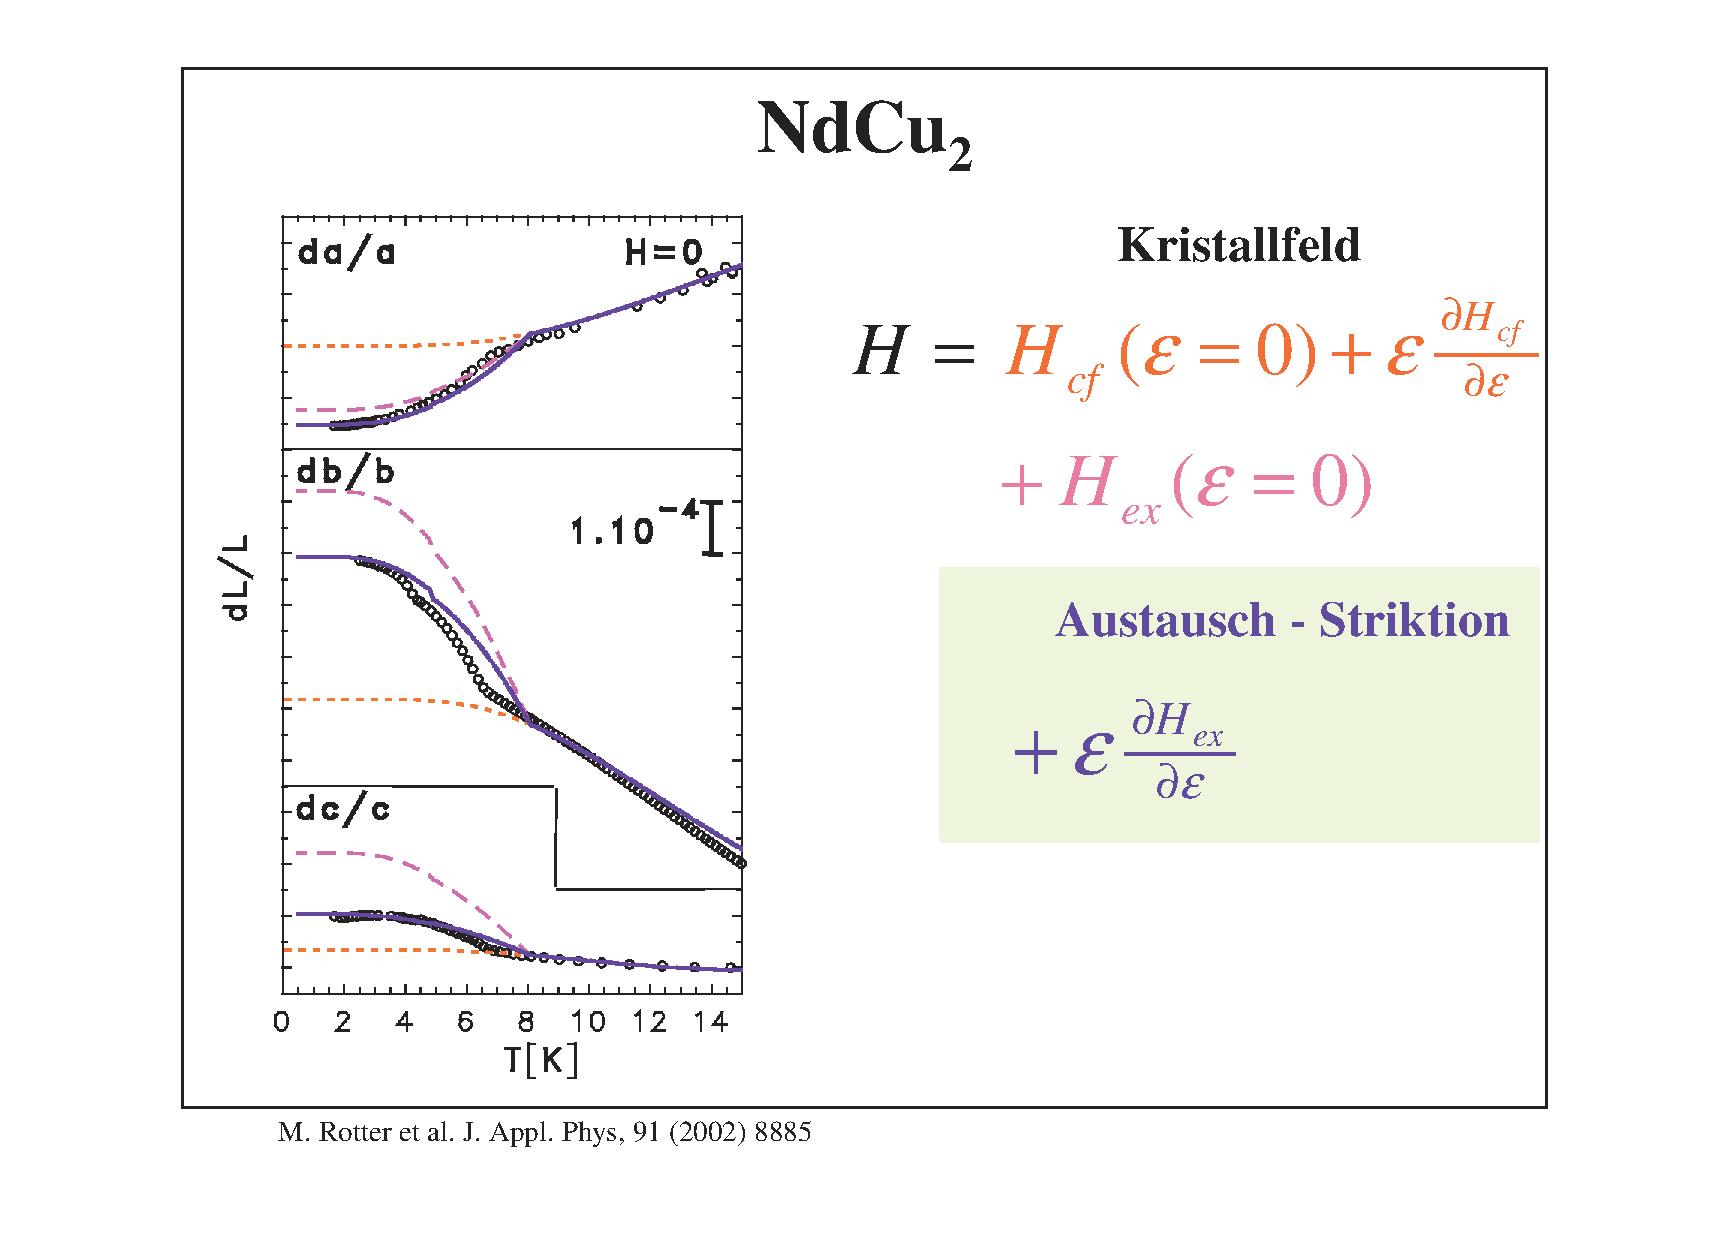
\includegraphics[angle=0, width=0.8\textwidth]{figsrc/magnetostriction_ndcu2.eps}
\end{center}
\caption{Calculated spontaneous magnetostriction of NdCu$_2$.}
\label{magnetostrictiongraphic}
\end{figure}

\begin{description}
\item [\prg mcphas.qvc]    the set of test q-vectors used for calculation of free energy.
                           Components of these q vectors refer to the reciprocal lattice $\vec a^*,\vec b^*,\vec c^*$.
\item [\prg mcphas.phs]    spin-configuration table of different types of spin-configurations. 
                            Note, in case of non-orthogonal axes the convention in these tables 
                            is $mb||\vec b$, $mc||(\vec a \times \vec b)$ and $ma$ perpendicular to $mb$ and $mc$.

                           {\em Note}: 
                           there is no natural criteria for deciding, if one spin-configuration is
			   different from another one. Therefore the list of ''different''
			   spin-configurations is dependent on the meaning of ''different''.
			   
			   The program {\prg McPhase} decides whether a spin-configuration is
			   different from another by a simple criteria, namely by the
			   angle between the spins. Comparing two spin configurations it calculates
			   the angle between corresponding spins and if for one spin the
			   angle is not small, the configuration is treated as a different
			   configuration. Therefore for example a ferromagnet with moments
			   in $a$ has a different spin configuration than a ferromagnet with
			   moments in $b$ direction. 
\item [\prg mcphas.sps]    $T-H$ dependence of spin-configuration. The spin configurations stored in this
                           file may be displayed using the program {\prg spins\index{spins}}, an example is given
			   in figure~\ref{spingraphic}.
                            Note, in case of non-orthogonal axes the convention for applied field $Ha, Hb,Hc$ and
                            also for the moment components $ma, mb, mc$ in these tables 
                            is $mb||\vec b$, $mc||(\vec a \times \vec b)$ and $ma$ perpendicular to $mb$ and $mc$.

\item [\prg mcphas.mf]     $T-H$ dependence of exchange field configuration, stored as $g_J \mu_B H_{xc}(i)$(unit is in meV)
                            for i=1,2,...,number of spins in magnetic unit cell.
                            Note, in case of non-orthogonal axes the convention for applied field $Ha, Hb,Hc$ and
                            also for the mean field components in these tables 
                            is $Hb||\vec b$, $Hc||(\vec a \times \vec b)$ and $Ha$ perpendicular to $Hb$ and $Hc$.
\item [\prg mcphas.fum]    free energy, magnetic energy (the derivative with respect to temperature gives the specific %%@
heat),
                           magnetisation data and (if cfield is used with higher order interactions)
                           expectation values of the Stevens Operators $<O_l^m>$ . As an example for the information
			   contained in this file the calculated magnetisation and magnetostriction of NdCu$_2$ is shown in
			   figures~\ref{magnetization} and ~\ref{magnetizationgraphic}.
                            Note, in case of non-orthogonal axes the convention for applied field $Ha, Hb,Hc$ and
                            also for the magnetisation components $ma,mb,mc$ in these tables 
                            is $Hb||\vec b$, $Hc||(\vec a \times \vec b)$ and $Ha$ perpendicular to $Hb$ and $Hc$.

\item [\prg mcphas1.j1 .j1 .j2 ...] 
               spin-spin correlation functions for sub-lattice 1 neighbour 1 2 ...
	       (linear combination is proportional to magnetostriction)
	       The spin-spin correlation functions for neighbour $k$ are defined by
	       the following sum of dyadic products:

	       \begin{equation}
	        \frac{1}{n}\sum_{s=1}^n <{\mbf J}^s> \times  <{\mbf J}^{s+k}>
	       \end{equation}
	       with $n$ being the number of moments in the magnetic unit cell.
	       Single ion and two-ion magnetostriction can be calculated using the $<O_l^m>$ and the
	       spin-spin correlation functions. As an example the magnetostriction analysis of
	       NdCu$_2$ is shown in figure~\ref{magnetostrictiongraphic}. For details 
             please refer to~\cite{rotter02-8885}.
                            Note, in case of non-orthogonal axes the convention for applied field $Ha, Hb,Hc$ and
                            also for the moment components in these tables 
                            is $Hb||\vec b$, $Hc||(\vec a \times \vec b)$ and $Ha$ perpendicular to $Hb$ and $Hc$.
\item [\prg mcphas.xyt]    phase diagram as x,y,T, H, phase-number j according to spin-configuration table
               given in mcphas.phs, a periodicity key, nettomoments <J>.
 Figure~\ref{phasediagramgraphic}
	       shows the phase diagram of NdCu$_2$ for magnetic fields parallel to the orthorhombic $b$-direction.
                            Note, in case of non-orthogonal axes the convention for applied field $Ha, Hb,Hc$ 
                             in these tables 
                            is $Hb||\vec b$, $Hc||(\vec a \times \vec b)$ and $Ha$ perpendicular to $Hb$ and $Hc$.
\item [\prg mcphas.hkl]    calculated (unpolarised) neutron diffraction data (the calculated magnetic intensities
    correspond to the magnetic structure + Polarisation factor. The
    Lorentz-factor , magnetic form factor and  instrumental corrections are not calculated.)
 As an example figure~\ref{neutintgraphic}
    shows the calculated temperature dependence of magnetic amplitudes for NdCu$_2$.
                           $h,k,l$ refer to the reciprocal lattice $\vec a^*,\vec b^*,\vec c^*$.
                            Note, in case of non-orthogonal axes the convention for applied field $Ha, Hb,Hc$ 
                             in these tables 
                            is $Hb||\vec b$, $Hc||(\vec a \times \vec b)$ and $Ha$ perpendicular to $Hb$ and $Hc$.
    
\item [\prg mcphasa.hkl]    Fourier Transform of the $a$-component of the magnetic Moments.
                           $h,k,l$ refer to the reciprocal lattice $\vec a^*,\vec b^*,\vec c^*$.
                            Note, in case of non-orthogonal axes the convention for applied field $Ha, Hb,Hc$ and
                            the magnetic moment component in these tables 
                            is $Hb||\vec b$, $Hc||(\vec a \times \vec b)$ and $Ha$ perpendicular to $Hb$ and $Hc$.
\item [\prg mcphasb.hkl]    Fourier Transform of the $b$-component of the magnetic Moments.
                           $h,k,l$ refer to the reciprocal lattice $\vec a^*,\vec b^*,\vec c^*$.
                            Note, in case of non-orthogonal axes the convention for applied field $Ha, Hb,Hc$ and
                            the magnetic moment component in these tables 
                            is $Hb||\vec b$, $Hc||(\vec a \times \vec b)$ and $Ha$ perpendicular to $Hb$ and $Hc$.
\item [\prg mcphasc.hkl]    Fourier Transform of the $c$-component of the magnetic Moments.
                           $h,k,l$ refer to the reciprocal lattice $\vec a^*,\vec b^*,\vec c^*$.
                            Note, in case of non-orthogonal axes the convention for applied field $Ha, Hb,Hc$ and
                            the magnetic moment component in these tables 
                            is $Hb||\vec b$, $Hc||(\vec a \times \vec b)$ and $Ha$ perpendicular to $Hb$ and $Hc$.
\end{description} 

\vspace{1cm}
{\em Exercises:}
\begin{itemize}
\item Look at the output files of {\prg McPhase}  in the directory
{\prg examples/ndcu2b\_new/results}.  At which magnetic field
the ferromagnetically aligned state is achieved (at $T=$2~K)?
\item
What is the propagation vector in the different antiferromagnetic phases at $T=$2~K ?
\end{itemize}


Note, in case of non-orthogonal axes the convention 
is $mb||\vec b$, $mc||(\vec a \times \vec b)$ and $ma$ perpendicular to $mb$ and $mc$.

\subsubsection{subdirectory {\prg ./results} - directory where calculated data is stored}

In order to be able to save the results of a calculation the directory {\prg ./results} has to
exist. Mind that all files in this directory will be overwritten without warning. 

\subsubsection{subdirectory {\prg ./fit} - experimental data for fit (optional) } 

In order that {\prg McPhase} can calculate the standard deviation between
 experimental data and the results of the simulation, some experimental data
 can be given in the subdirectory {\prg ./fit}. The filenames and the data-format
 are the same as the output files of {\prg McPhas}, e.g. {\prg mcphas.fum}, {\prg mcphas.hkl}
 etc. {\prg McPhase} looks into the directory {\prg ./fit} and if it finds any
 of these files, the standard deviation is increased correspondingly. 

What measurement data can be used to calculate a standard deviation ?

\begin{description}
\item[{\prg mcphas.fum}] if given in column 11, 12, 13 in {\prg ./fit/mcphas.fum} the
            magnetisation in the $a$, $b$ and $c$ direction is used for calculation
	    of the standard deviation sta. The standard deviation is calculated
	    as ${\rm sta}=\sum_{\rm data points i} ({\mbf m}_i^{calc}-{\mbf m}_i^{meas})^2$.
	    All three components of the magnetic moment have to be given and are used.

\end{description}

Note that the measured data has to be given in those (H-T) points which are 
calculated by mcphas\index{mcphas} in order to be used by the program to increase {\prg sta}.
It is usually most effective to fit only few data points, because a large set
of data points will not improve the quality of the fit and only require a large
amount of calculation time.



\subsection{Starting a simulation}
\label{start}

To start the simulation goto the directory containing the
input files {\prg mcphas.ini, mcphas.j, etc. } and type

\begin{description}
\item[\prg mcphas] to run the program generating stepwise $H-T$ values 
              in a loop given by {\prg mcphas.ini\index{mcphas.ini}} (you can also press the
              symbol in the {\prg McPhase - Explorer} window).
\item[\prg mcphas\index{mcphas} [file]]  to run the program with an input file --   
             {\prg file} contains T ha hb hc values to be calculated 
             if [file] is not given, xmin xmax xstep (xT xHa xHb xHc)
             ymin ymax ystep (yT yHa yHb yHc) is read from file {\prg mcphas.ini\index{mcphas.ini}}
	     and phase diagram is calculated
\item[\prg mcphas\index{mcphas} -h]  to  print help and version of {\prg McPhas}.
\item[\prg mcphas\index{mcphas} -stamax 14]  end mcphas\index{mcphas} if standard deviation exceeds 14.
\item[\prg mcphas\index{mcphas} -a] avoid overwriting output files in results, append new results to existing files
\item[\prg mcphas\index{mcphas} -v]  to  enable verbose mode with lots of messages of {\prg McPhas}. Specifically
the verbose mode enables the following features:
  \begin{itemize}
			          \item more information is printed out, 
			          \item the q-vectors file {\prg ./results/mcphas.qvc} will contain 
				    the explicit spin configurations
			          \item the display\index{display} on screen (ghostview window using 
				     {\prg ./results/.sps.eps}) will be updated not only 
				    when a H-T point has been finished but always 
				    when a structure with smaller free energy 
				    has been stabilised
  \end{itemize}
\item[\prg mcphasit\index{mcphas}] to start mcphase in commandline mode without opening any window
\end{description}

\vspace{1cm}
{\em Exercises:}
\begin{itemize}
\item Look at the input files for {\prg McPhase} given in the directory
{\prg examples/ndcu2b\_new}.  How many atoms are contained in the crystallographic basis ?
\item
Start the simulation by typing the command {\prg mcphas}.
\end{itemize}



\subsection{Options for a running simulation}
... when the program is running, the options in the main window
can be changed. Pressing ''displayall'' displays the current spin-configuration
at each iteration step. Pressing ''log fe vs Q'' appends free energy vs Q
data to {\prg mcphas.log} for every ($T-H$) point.


The file {\prg ./results/.spins.eps} is used to show the information about the currently calculated
spin structure on the screen using the postscript file viewer ghostview.

The file {\prg ./results/.mcphas.fum} contains the information of the magnetisation curve
which is currently calculated. This information is automatically displayed on the screen.


The program {\prg display} (see section \ref{display}) can be used 
for the online display\index{display} of any other
curve(s).


\subsection{Output Files - {\prg mcphas.qvc,phs,sps,mf,fum,j1...,xyt,hkl} }\label{outputfiles}
 (in directory ./results/ after a simulation run) 

\begin{figure}[htb]%h=here, t=top, b=bottom, p=separate figure page
\begin{center}\leavevmode
\includegraphics[angle=0, width=0.3\textwidth]{figsrc/magnetization_ndcu2.ps}
\end{center}
\caption{Calculated magnetisation of NdCu$_2$ for field parallel to the orthorhombic $b$-direction.}
\label{magnetization}
\end{figure}

\begin{figure}[htb]%h=here, t=top, b=bottom, p=separate figure page
\begin{center}\leavevmode
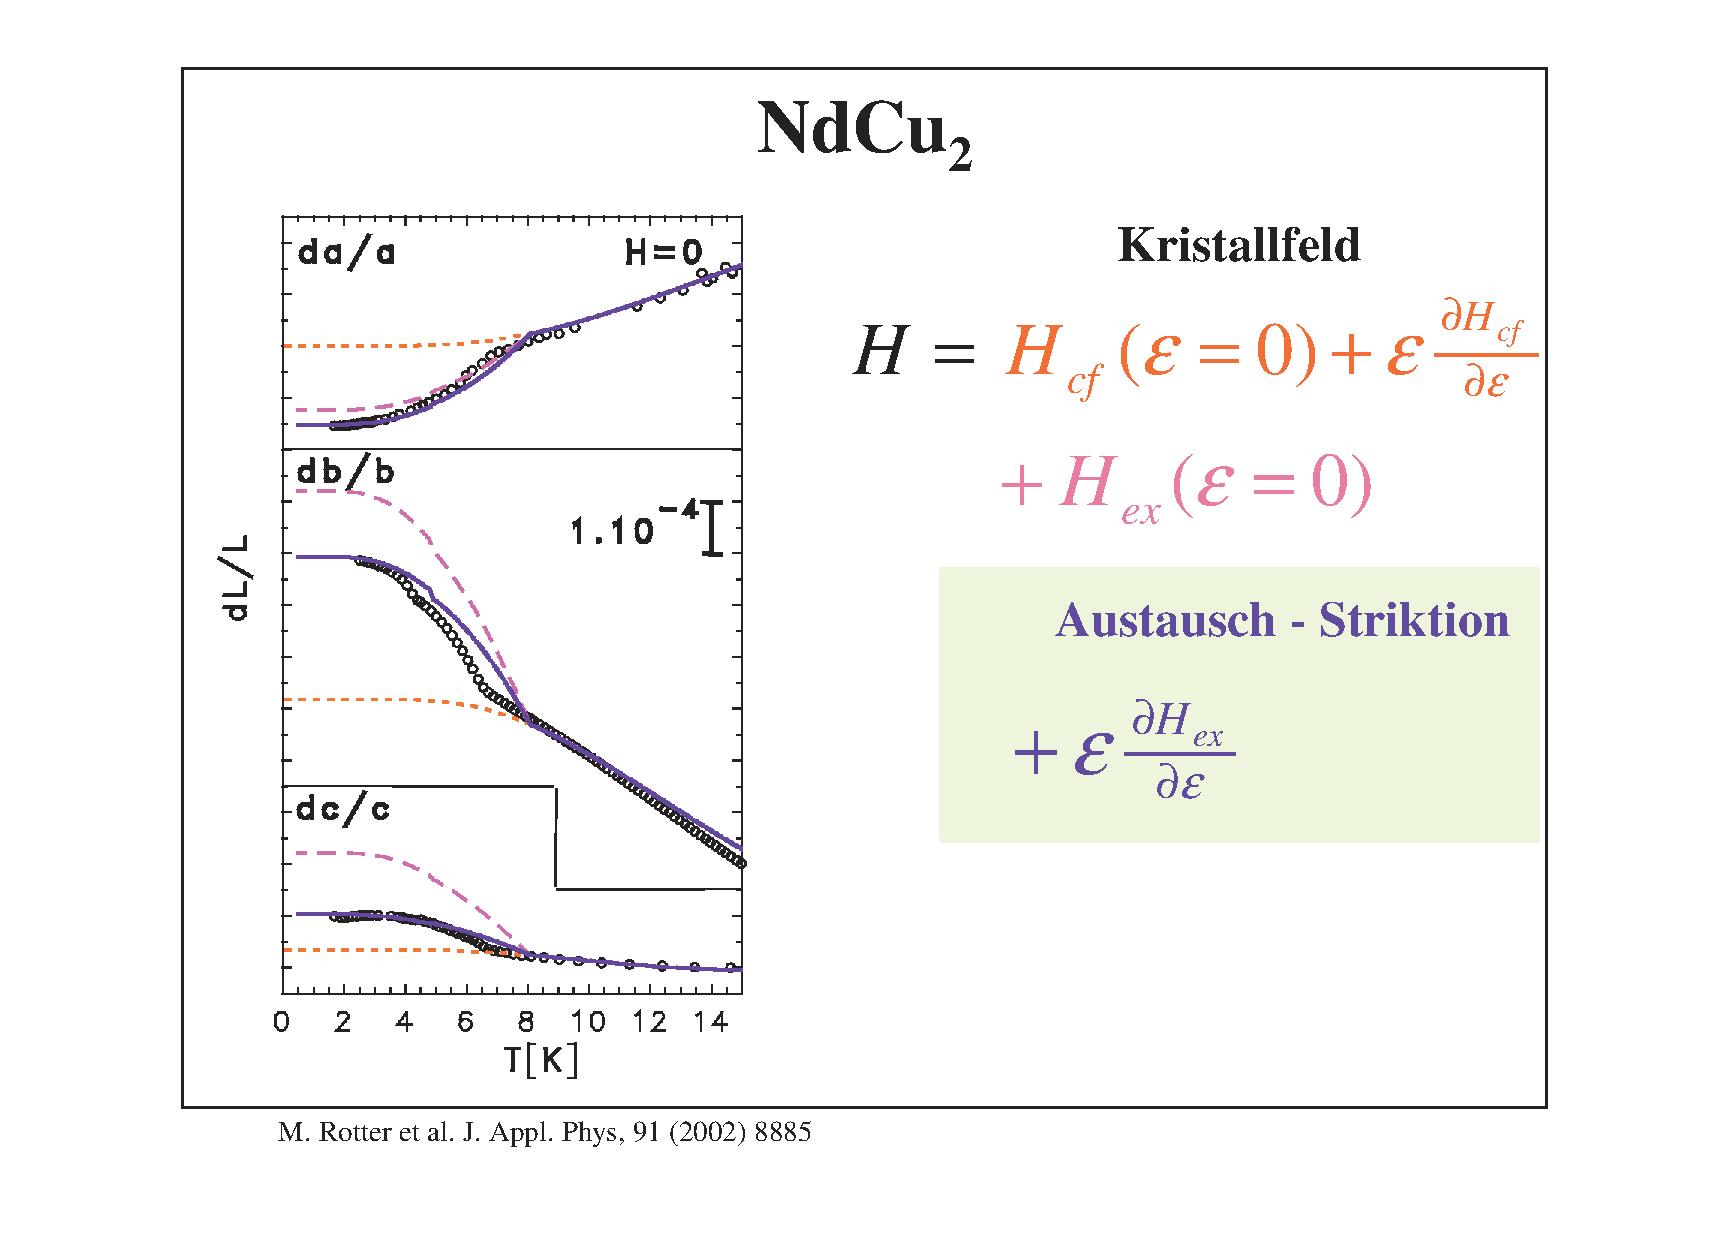
\includegraphics[angle=0, width=0.8\textwidth]{figsrc/magnetostriction_ndcu2.eps}
\end{center}
\caption{Calculated spontaneous magnetostriction of NdCu$_2$.}
\label{magnetostrictiongraphic}
\end{figure}

\begin{description}
\item [\prg mcphas.qvc]    the set of test q-vectors used for calculation of free energy.
                           Components of these q vectors refer to the reciprocal lattice $\vec a^*,\vec b^*,\vec c^*$.
\item [\prg mcphas.phs]    spin-configuration table of different types of spin-configurations. 
                            Note, in case of non-orthogonal axes the convention in these tables 
                            is $mb||\vec b$, $mc||(\vec a \times \vec b)$ and $ma$ perpendicular to $mb$ and $mc$.

                           {\em Note}: 
                           there is no natural criteria for deciding, if one spin-configuration is
			   different from another one. Therefore the list of ''different''
			   spin-configurations is dependent on the meaning of ''different''.
			   
			   The program {\prg McPhase} decides whether a spin-configuration is
			   different from another by a simple criteria, namely by the
			   angle between the spins. Comparing two spin configurations it calculates
			   the angle between corresponding spins and if for one spin the
			   angle is not small, the configuration is treated as a different
			   configuration. Therefore for example a ferromagnet with moments
			   in $a$ has a different spin configuration than a ferromagnet with
			   moments in $b$ direction. 
\item [\prg mcphas.sps]    $T-H$ dependence of spin-configuration. The spin configurations stored in this
                           file may be displayed using the program {\prg spins\index{spins}}, an example is given
			   in figure~\ref{spingraphic}.
                            Note, in case of non-orthogonal axes the convention for applied field $Ha, Hb,Hc$ and
                            also for the moment components $ma, mb, mc$ in these tables 
                            is $mb||\vec b$, $mc||(\vec a \times \vec b)$ and $ma$ perpendicular to $mb$ and $mc$.

\item [\prg mcphas.mf]     $T-H$ dependence of exchange field configuration, stored as $g_J \mu_B H_{xc}(i)$(unit is in meV)
                            for i=1,2,...,number of spins in magnetic unit cell.
                            Note, in case of non-orthogonal axes the convention for applied field $Ha, Hb,Hc$ and
                            also for the mean field components in these tables 
                            is $Hb||\vec b$, $Hc||(\vec a \times \vec b)$ and $Ha$ perpendicular to $Hb$ and $Hc$.
\item [\prg mcphas.fum]    free energy, magnetic energy (the derivative with respect to temperature gives the specific %%@
heat),
                           magnetisation data and (if cfield is used with higher order interactions)
                           expectation values of the Stevens Operators $<O_l^m>$ . As an example for the information
			   contained in this file the calculated magnetisation and magnetostriction of NdCu$_2$ is shown in
			   figures~\ref{magnetization} and ~\ref{magnetizationgraphic}.
                            Note, in case of non-orthogonal axes the convention for applied field $Ha, Hb,Hc$ and
                            also for the magnetisation components $ma,mb,mc$ in these tables 
                            is $Hb||\vec b$, $Hc||(\vec a \times \vec b)$ and $Ha$ perpendicular to $Hb$ and $Hc$.

\item [\prg mcphas1.j1 .j1 .j2 ...] 
               spin-spin correlation functions for sub-lattice 1 neighbour 1 2 ...
	       (linear combination is proportional to magnetostriction)
	       The spin-spin correlation functions for neighbour $k$ are defined by
	       the following sum of dyadic products:

	       \begin{equation}
	        \frac{1}{n}\sum_{s=1}^n <{\mbf J}^s> \times  <{\mbf J}^{s+k}>
	       \end{equation}
	       with $n$ being the number of moments in the magnetic unit cell.
	       Single ion and two-ion magnetostriction can be calculated using the $<O_l^m>$ and the
	       spin-spin correlation functions. As an example the magnetostriction analysis of
	       NdCu$_2$ is shown in figure~\ref{magnetostrictiongraphic}. For details 
             please refer to~\cite{rotter02-8885}.
                            Note, in case of non-orthogonal axes the convention for applied field $Ha, Hb,Hc$ and
                            also for the moment components in these tables 
                            is $Hb||\vec b$, $Hc||(\vec a \times \vec b)$ and $Ha$ perpendicular to $Hb$ and $Hc$.
\item [\prg mcphas.xyt]    phase diagram as x,y,T, H, phase-number j according to spin-configuration table
               given in mcphas.phs, a periodicity key, nettomoments <J>.
 Figure~\ref{phasediagramgraphic}
	       shows the phase diagram of NdCu$_2$ for magnetic fields parallel to the orthorhombic $b$-direction.
                            Note, in case of non-orthogonal axes the convention for applied field $Ha, Hb,Hc$ 
                             in these tables 
                            is $Hb||\vec b$, $Hc||(\vec a \times \vec b)$ and $Ha$ perpendicular to $Hb$ and $Hc$.
\item [\prg mcphas.hkl]    calculated (unpolarised) neutron diffraction data (the calculated magnetic intensities
    correspond to the magnetic structure + Polarisation factor. The
    Lorentz-factor , magnetic form factor and  instrumental corrections are not calculated.)
 As an example figure~\ref{neutintgraphic}
    shows the calculated temperature dependence of magnetic amplitudes for NdCu$_2$.
                           $h,k,l$ refer to the reciprocal lattice $\vec a^*,\vec b^*,\vec c^*$.
                            Note, in case of non-orthogonal axes the convention for applied field $Ha, Hb,Hc$ 
                             in these tables 
                            is $Hb||\vec b$, $Hc||(\vec a \times \vec b)$ and $Ha$ perpendicular to $Hb$ and $Hc$.
    
\item [\prg mcphasa.hkl]    Fourier Transform of the $a$-component of the magnetic Moments.
                           $h,k,l$ refer to the reciprocal lattice $\vec a^*,\vec b^*,\vec c^*$.
                            Note, in case of non-orthogonal axes the convention for applied field $Ha, Hb,Hc$ and
                            the magnetic moment component in these tables 
                            is $Hb||\vec b$, $Hc||(\vec a \times \vec b)$ and $Ha$ perpendicular to $Hb$ and $Hc$.
\item [\prg mcphasb.hkl]    Fourier Transform of the $b$-component of the magnetic Moments.
                           $h,k,l$ refer to the reciprocal lattice $\vec a^*,\vec b^*,\vec c^*$.
                            Note, in case of non-orthogonal axes the convention for applied field $Ha, Hb,Hc$ and
                            the magnetic moment component in these tables 
                            is $Hb||\vec b$, $Hc||(\vec a \times \vec b)$ and $Ha$ perpendicular to $Hb$ and $Hc$.
\item [\prg mcphasc.hkl]    Fourier Transform of the $c$-component of the magnetic Moments.
                           $h,k,l$ refer to the reciprocal lattice $\vec a^*,\vec b^*,\vec c^*$.
                            Note, in case of non-orthogonal axes the convention for applied field $Ha, Hb,Hc$ and
                            the magnetic moment component in these tables 
                            is $Hb||\vec b$, $Hc||(\vec a \times \vec b)$ and $Ha$ perpendicular to $Hb$ and $Hc$.
\end{description} 

\vspace{1cm}
{\em Exercises:}
\begin{itemize}
\item Look at the output files of {\prg McPhase}  in the directory
{\prg examples/ndcu2b\_new/results}.  At which magnetic field
the ferromagnetically aligned state is achieved (at $T=$2~K)?
\item
What is the propagation vector in the different antiferromagnetic phases at $T=$2~K ?
\end{itemize}



\subsubsection{{\prg mcphas.tst\index{mcphas.tst}} - input file of test spin-configurations (optional)}
This file is optional and contains
some test momentum configurations to be used for the calculation
             of the free energy. Mind that
\begin{itemize}
\item  in the file header the number of atoms in the primitive
       crystallographic unit cell and the number of components
       of the spin vector have to be given.
\item  at the end of the
 file there must be no empty lines !
\end{itemize}

The momentum - configurations tables always refer to spins sitting on
the primitive lattice ${\mbf r}_i$. If more than one atom is in
the primitive basis, the momentum gets $3n$ components ($n=$ number
of atoms in the crystallographic basis). See {\prg ./examples/ndcu2b\_new/} for
examples of a two atom basis. Units of these tables are that of total 
angular momentum $<J>$.

\subsubsection{Example {\prg mcphas.tst\index{mcphas.tst}} file  for a simple antiferromagnet}

Here is the file {\prg mcphas.tst\index{mcphas.tst}} for the simple antiferromagnet example
describing some spin configurations
to be used as starting values for the mean field process:

\section{{\prg mcphas} - calculation of thermodynamic properties (Magnetisation, Susceptibility, Specific Heat, Neutron %%@
Diffraction, etc.)}
\label{runmcphas}

In order to perform calculations beyond the capabilities of {\prg cfield\index{cfield}} it is necessary
to use the program {\prg mcphas}. 
\begin{itemize}
\item As a first step it is possible to
calculate the thermodynamic properties such as magnetisation or specific heat
considering only single ion effects. In this case all the exchange parameters
have to be set to zero in {\prg mcphas.j\index{mcphas.j}}. 
\item for more advanced calculations the two - ion interactions have to be
considered and may lead to magnetic order. {\prg mcphas} can perform 
calculations in the ordered state in the following way: for 
a given temperature $T$ and magnetic field $\mbf H$ (vector)
several possible magnetic structures are stabilised
by a mean field algorithm and the free energy is 
calculated. The initial values for this mean-field procedure are
modified by a Monte Carlo process.


The temperature and magnetic field is varied during the calculation
and thereby it is possible to map out the magnetic phase diagram.
\end{itemize}

The program produces a plot of the stabilised magnetic
structures and the magnetisation on screen, the
output files contain additional information 
such as calculated magnetoelastic and  neutron-scattering
data. Several graphic programs easy the visualisation of the
calculated data (section~\ref{graphics}).



\subsection{Input Files}
The program {\prg McPhase} needs the following input files (all in the same directory)
 in order to run:

\begin{enumerate}
\item {\prg mcphas.ini\index{mcphas.ini}}
 - controlling the algorithm
\item {\prg mcphas.j\index{mcphas.j}}
  - lattice and exchange parameters
\item {\prg mcphas.tst\index{mcphas.tst}(optional)}  - test spin configurations
\item {\prg single-ion property files}
\item {\prg directory ./results/}
 - directory where calculated data is stored
\item {\prg directory ./fit} - experimental data for fit (optional)
\end{enumerate}


 All
 of these input files have to be in one directory and the program
has to be started in this directory. The results of the simulation
are then stored in the  subdirectory ./results/, which must exist before starting
the program 
... see directory ./examples/ for some examples.
 In order to prepare these files
for a new calculation it is best to take them from an example, copy the files
to a new directory and make the
modifications  to adapt them to the new problem.

\subsubsection{Example - a simple antiferromagnet}

In the following description of the input files we will always refer
to a simple example: a simple antiferromagnet
on a primitive orthorhombic lattice. The first time user
will thus have a simple example to follow, all corresponding
files are given in the directory {\prg tutorial/03magnetic\_phases\_mcphas/simpleAF}.
 

\subsubsection{{\prg mcphas.ini\index{mcphas.ini}} - controlling the algorithm}
   Initial file containing algorithm control parameters, for instance the range and spacing of
   propagation vectors Q or the number of Monte Carlo trials for initial spin configurations
    - {\em mind}: this
   file is rewritten and reread  when running the program and may be changed by the
   user in order to manipulate the running simulation.

{\prg mcphas.ini\index{mcphas.ini}} consists of several sections:
\begin{description}
\item [MCPHASE RUNTIME CONTROL:] this section contains the parameters
controlling the status of the calculation.
\item [XY PHASEDIAGRAM PARAMETERS:] here the temperature and field range and
step widths of the calculation are specified.
The definition of the x and y
axis in terms of temperature and magnetic field is followed by the
corresponding range and step width. An offset may be given for all
field and temperature values.
Note that for most cases of interest
this offset is zero (T0=0, Ha0=0, Hb0=0, Hc0=0).
 For the simple case of calculating a Temperature-Field phase diagram
 It is just necessary to set xT=1 and give the temperature range by
xmin/xmax/xstep. For field in b direction then just set yHb=1 and 
define the range in ymin/ymax/ystep.
In case of non-orthogonal axes the applied magnetic field
components $Ha, Hb, Hc$ refer to the orthogonal coordinate system
defined with respect to the nonorthogonal lattice $\mbf a,\mbf b,\mbf c$ as
$Hb||\mbf b$, $Hc||(\mbf a \times \mbf b)$ and $Ha$ perpendicular to $Hb$ and $Hc$.

\item [GENERATION OF SPINCONFIGURATIONS:] at the beginning of the program
some initial values of spin configurations are generated from a set of 
propagation vectors. This section defines the range of propagation vectors
and the step width.
Depending on the value of the propagation Q with respect to the primitive reciprocal lattice
1-, 2- or 3-dimensional simulations of magnetic lattices
are possible. It is advisable to 
think carefully about the chosen range and spacing of Q vectors in order
to limit calculation time.
 
For example a good starting point is to begin with a calculation with large
step widths (e.g. 0.1)  covering the Brillouin zone. This should give an idea
of the propagation vectors which are stabilised. An advanced calculation
could then fine tune the propagation and determine its accurate value (using
small step widths in a limited area of the zone).
The verbose option of {\prg mcphas} allows to inspect the propagation vectors
which are actually used in the calculation.
Trick: in order to get a quick overview of the
q-vector range covered by the mcphas\index{mcphas} simulation start mcphas, exit and 
just type {\prg felog ./results/mcphas.qvc} (need {\prg perl,perldl,pdl,pgplot} packages).

In order to limit calculation time, the maximum periodicity
of the magnetic unit cell with respect to the crystallographic unit cell 
(maxqperiod) and the maximum number of spins in the magnetic unit cell 
(maxnofspins) can be limited. Also the maximum number of test spin configurations
in the internal table can be limited (maxnoftestspincf).
A critical feature with respect to calculation time is also the number of
spin configurations which are generated by a random process from a tabulated
SPINCONFIGURATIONS during the calculation. 

In summary the variables in this section are mainly important to adapt the
program to a given computer system with finite speed. They have to be set
to optimise between speed and accuracy of the calculation. In order to
find appropriate values it is best to perform some calculations 
and restrict the parameters step by step if insufficient speed is obtained.
Also the examples included in the program package may serve as starting
points.

\item [PARAMETERS FOR SUB FECALC SELFCONSISTENCY PROCESS:] the most important
procedure in the module {\prg mcphas} is the sub fecalc. In this part of the 
program the self consistent calculation of the magnetic moment configuration
is performed as shown schematically in fig.~\ref{fecalc}. 
In the mean field approximation the Hamiltonian~(\ref{hamilton}) is approximated
by

\begin{equation}
 {\mathcal H}=\sum_n H_{SI}^n + E_{corr}
\end{equation}

with the single ion Hamiltonian (in case of module {\prg so1ion\index{so1ion}})

\begin{equation}
H_{SI}^n=  B_l^m O_{lm}({\mbf J}^n) 
	     - g_{Jn} \mu_B {\mbf J}^n {\mbf H^n_{eff}} 
\end{equation}

and the correction term

\begin{equation}
E_{corr}=\frac{1}{2}\sum_{n} g_{Jn} \mu_B \langle {\mbf J}^n
 \rangle (\mbf H^n_{eff}-\mbf H) 
\end{equation}

and with the mean fields $ \mbf H^n_{eff}$ given by

\begin{equation}\label{meanfield}
\mbf H^n_{eff}=\mbf H + \mbf H^n_{xc}=\mbf H+\sum_{{\mbf G'}n'} \frac{{\mathcal J}
(\mbf r_n-(\mbf G'+\mbf r_{n'}))}{g_{Jn}\mu_B } \langle{\mbf
J}^{n'}\rangle
\end{equation}

These mean fields and the moments $\langle \mbf J^n \rangle$ 
are determined in a self consistent
way. For a given magnetic unit cell and initial configuration 
of magnetic moments
the mean fields are calculated according to equation~(\ref{meanfield}). 
Then, for each
magnetic ion the single ion property module is taken 
and the magnetic moment $\langle \mbf J^n \rangle$ is 
calculated from it's mean field. The mean fields are used again in equation~(\ref{meanfield})
and so on .... until convergence is reached. 
Then, the free energy ($f=-kT\sum_n \ln(z_n) + E_{corr}$ ) 
of the stabilised
configuration is calculated (this is why this sub is called {\prg fecalc}). 
The free energies of a lot of different stabilised configurations have to
be compared in order to find out which configuration has lowest free energy, i.e.
is stable in thermal  equilibrium.

It may happen that this process does
not converge due to bad choice of the initial configuration, therefore a maximum number
of mean field loops has to be given by the user.
The results of a calculation may be significantly influenced by
changing parameters such as the maximum number of iteration loops 
in this section. 
In fact the simulation is always a compromise of calculation time and accuracy: if only
a few initial spin configurations are tried at each (H-T) point, the calculation speed is
fast, however it is possible that the program misses the magnetic structure with the
lowest free energy. The same holds if other critical parameters of the simulation are
restricted too much.
 

\item [OUTPUT OF PHYSICAL PROPERTIES:]
Some options for the output of the calculation can be changed in this section.
\end{description}

\begin{figure}[hb]
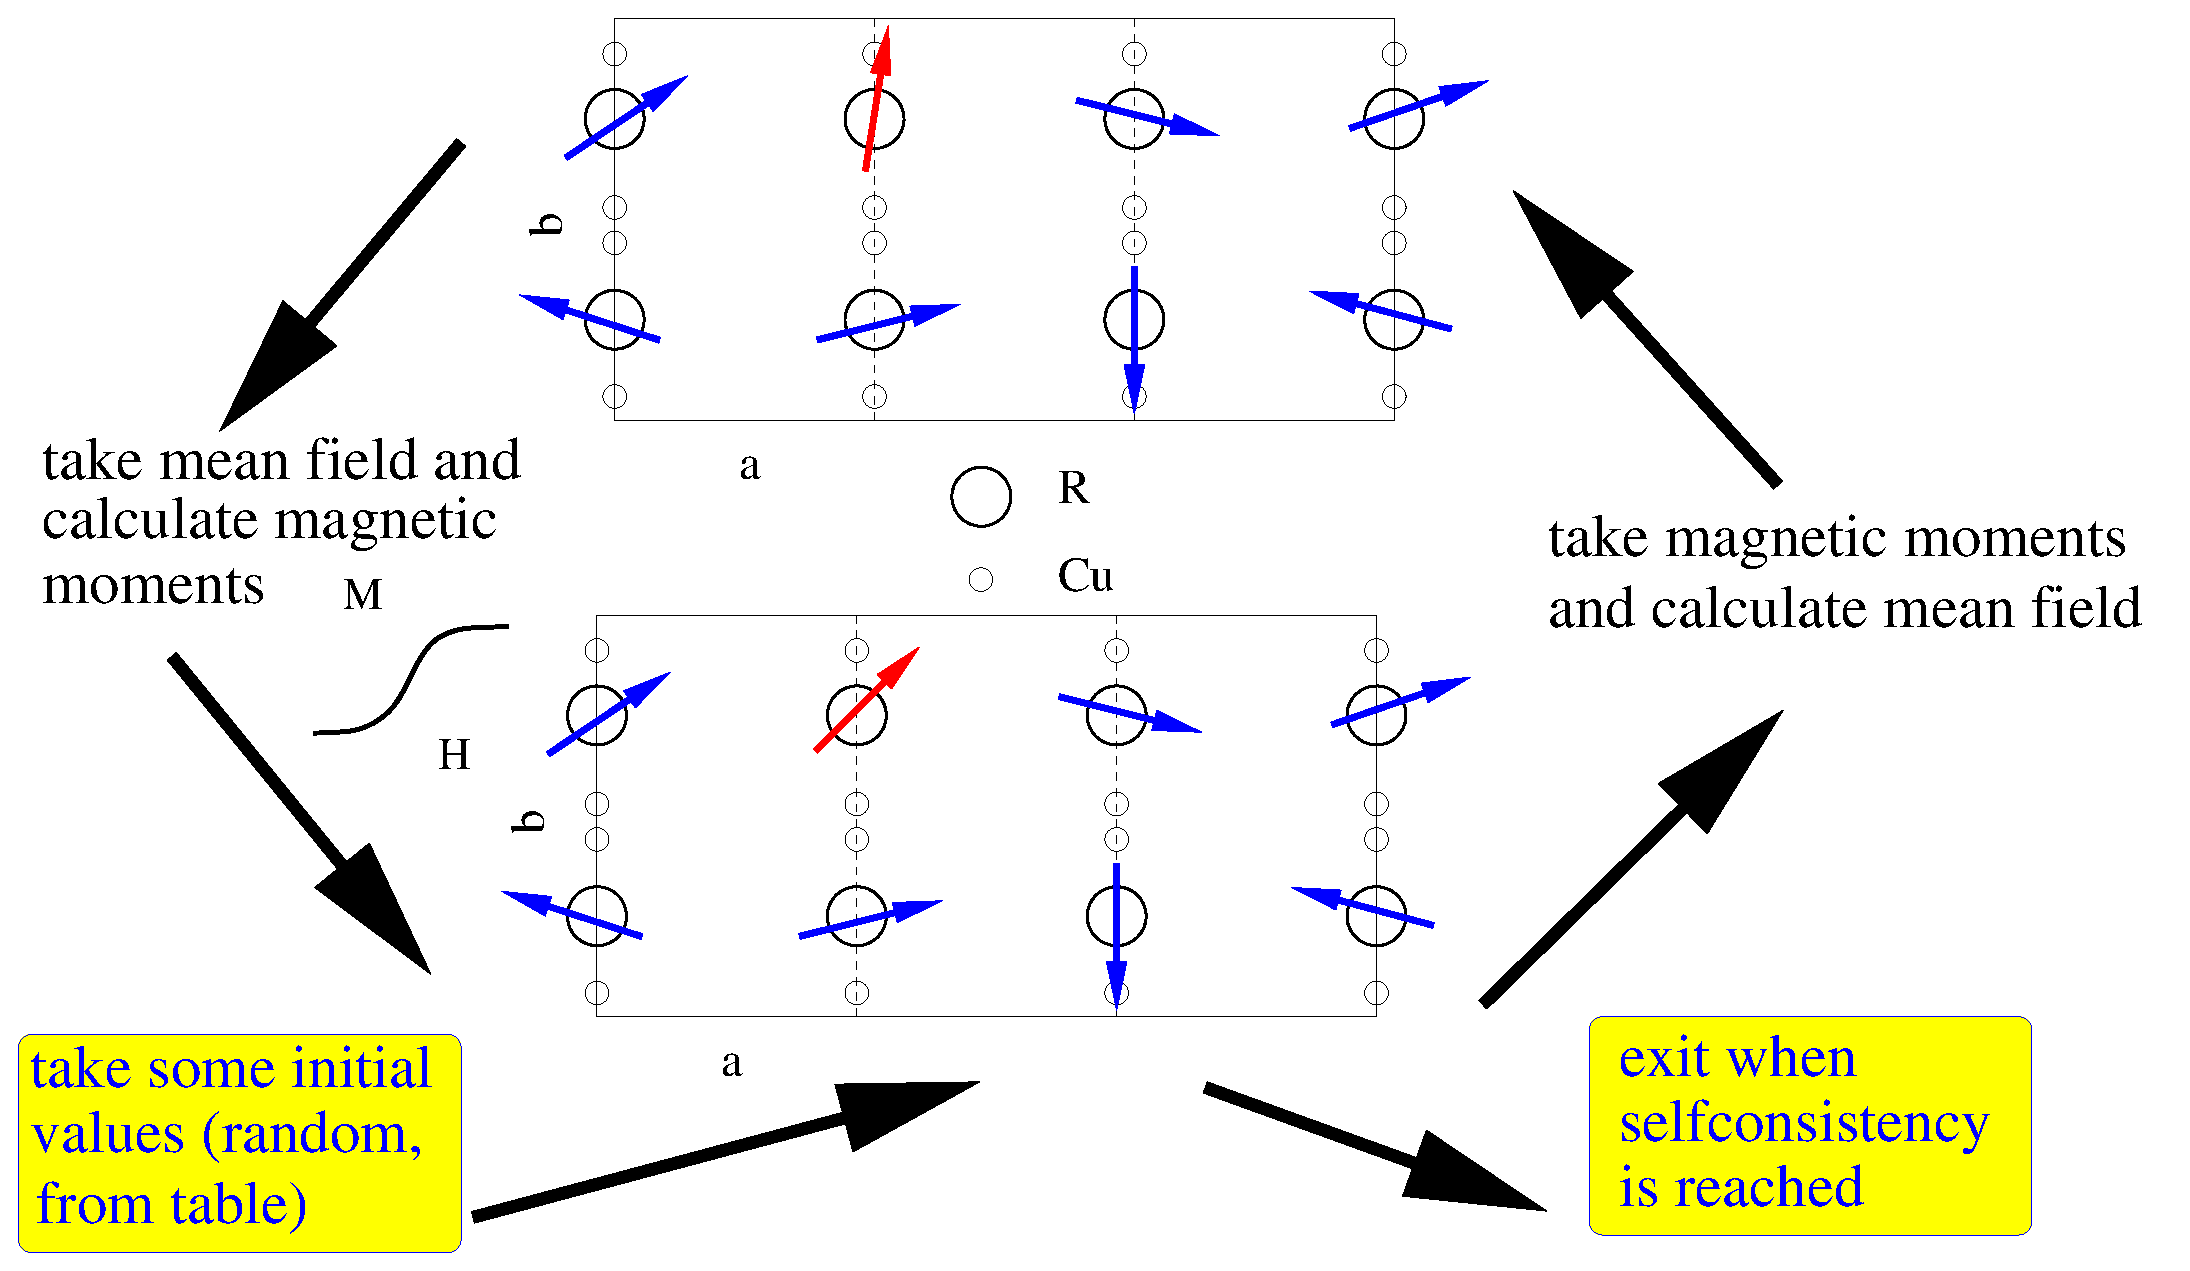
\includegraphics[angle=0,width=0.9\columnwidth]{figsrc/fecalc.eps}
\caption{\label{fecalc}Mean field process of sub {\prg fecalc}.}
\end{figure}

 
\subsubsection{Example {\prg mcphas.ini\index{mcphas.ini}} file for a simple antiferromagnet}

Here is an example of {\prg mcphas.ini\index{mcphas.ini}}, the comments describe the meaning of the different
parameters:

\section{{\prg mcphas} - calculation of thermodynamic properties (Magnetisation, Susceptibility, Specific Heat, Neutron %%@
Diffraction, etc.)}
\label{runmcphas}

In order to perform calculations beyond the capabilities of {\prg cfield\index{cfield}} it is necessary
to use the program {\prg mcphas}. 
\begin{itemize}
\item As a first step it is possible to
calculate the thermodynamic properties such as magnetisation or specific heat
considering only single ion effects. In this case all the exchange parameters
have to be set to zero in {\prg mcphas.j\index{mcphas.j}}. 
\item for more advanced calculations the two - ion interactions have to be
considered and may lead to magnetic order. {\prg mcphas} can perform 
calculations in the ordered state in the following way: for 
a given temperature $T$ and magnetic field $\mbf H$ (vector)
several possible magnetic structures are stabilised
by a mean field algorithm and the free energy is 
calculated. The initial values for this mean-field procedure are
modified by a Monte Carlo process.


The temperature and magnetic field is varied during the calculation
and thereby it is possible to map out the magnetic phase diagram.
\end{itemize}

The program produces a plot of the stabilised magnetic
structures and the magnetisation on screen, the
output files contain additional information 
such as calculated magnetoelastic and  neutron-scattering
data. Several graphic programs easy the visualisation of the
calculated data (section~\ref{graphics}).



\subsection{Input Files}
The program {\prg McPhase} needs the following input files (all in the same directory)
 in order to run:

\begin{enumerate}
\item {\prg mcphas.ini\index{mcphas.ini}}
 - controlling the algorithm
\item {\prg mcphas.j\index{mcphas.j}}
  - lattice and exchange parameters
\item {\prg mcphas.tst\index{mcphas.tst}(optional)}  - test spin configurations
\item {\prg single-ion property files}
\item {\prg directory ./results/}
 - directory where calculated data is stored
\item {\prg directory ./fit} - experimental data for fit (optional)
\end{enumerate}


 All
 of these input files have to be in one directory and the program
has to be started in this directory. The results of the simulation
are then stored in the  subdirectory ./results/, which must exist before starting
the program 
... see directory ./examples/ for some examples.
 In order to prepare these files
for a new calculation it is best to take them from an example, copy the files
to a new directory and make the
modifications  to adapt them to the new problem.

\subsubsection{Example - a simple antiferromagnet}

In the following description of the input files we will always refer
to a simple example: a simple antiferromagnet
on a primitive orthorhombic lattice. The first time user
will thus have a simple example to follow, all corresponding
files are given in the directory {\prg tutorial/03magnetic\_phases\_mcphas/simpleAF}.
 

\subsubsection{{\prg mcphas.ini\index{mcphas.ini}} - controlling the algorithm}
   Initial file containing algorithm control parameters, for instance the range and spacing of
   propagation vectors Q or the number of Monte Carlo trials for initial spin configurations
    - {\em mind}: this
   file is rewritten and reread  when running the program and may be changed by the
   user in order to manipulate the running simulation.

{\prg mcphas.ini\index{mcphas.ini}} consists of several sections:
\begin{description}
\item [MCPHASE RUNTIME CONTROL:] this section contains the parameters
controlling the status of the calculation.
\item [XY PHASEDIAGRAM PARAMETERS:] here the temperature and field range and
step widths of the calculation are specified.
The definition of the x and y
axis in terms of temperature and magnetic field is followed by the
corresponding range and step width. An offset may be given for all
field and temperature values.
Note that for most cases of interest
this offset is zero (T0=0, Ha0=0, Hb0=0, Hc0=0).
 For the simple case of calculating a Temperature-Field phase diagram
 It is just necessary to set xT=1 and give the temperature range by
xmin/xmax/xstep. For field in b direction then just set yHb=1 and 
define the range in ymin/ymax/ystep.
In case of non-orthogonal axes the applied magnetic field
components $Ha, Hb, Hc$ refer to the orthogonal coordinate system
defined with respect to the nonorthogonal lattice $\mbf a,\mbf b,\mbf c$ as
$Hb||\mbf b$, $Hc||(\mbf a \times \mbf b)$ and $Ha$ perpendicular to $Hb$ and $Hc$.

\item [GENERATION OF SPINCONFIGURATIONS:] at the beginning of the program
some initial values of spin configurations are generated from a set of 
propagation vectors. This section defines the range of propagation vectors
and the step width.
Depending on the value of the propagation Q with respect to the primitive reciprocal lattice
1-, 2- or 3-dimensional simulations of magnetic lattices
are possible. It is advisable to 
think carefully about the chosen range and spacing of Q vectors in order
to limit calculation time.
 
For example a good starting point is to begin with a calculation with large
step widths (e.g. 0.1)  covering the Brillouin zone. This should give an idea
of the propagation vectors which are stabilised. An advanced calculation
could then fine tune the propagation and determine its accurate value (using
small step widths in a limited area of the zone).
The verbose option of {\prg mcphas} allows to inspect the propagation vectors
which are actually used in the calculation.
Trick: in order to get a quick overview of the
q-vector range covered by the mcphas\index{mcphas} simulation start mcphas, exit and 
just type {\prg felog ./results/mcphas.qvc} (need {\prg perl,perldl,pdl,pgplot} packages).

In order to limit calculation time, the maximum periodicity
of the magnetic unit cell with respect to the crystallographic unit cell 
(maxqperiod) and the maximum number of spins in the magnetic unit cell 
(maxnofspins) can be limited. Also the maximum number of test spin configurations
in the internal table can be limited (maxnoftestspincf).
A critical feature with respect to calculation time is also the number of
spin configurations which are generated by a random process from a tabulated
SPINCONFIGURATIONS during the calculation. 

In summary the variables in this section are mainly important to adapt the
program to a given computer system with finite speed. They have to be set
to optimise between speed and accuracy of the calculation. In order to
find appropriate values it is best to perform some calculations 
and restrict the parameters step by step if insufficient speed is obtained.
Also the examples included in the program package may serve as starting
points.

\item [PARAMETERS FOR SUB FECALC SELFCONSISTENCY PROCESS:] the most important
procedure in the module {\prg mcphas} is the sub fecalc. In this part of the 
program the self consistent calculation of the magnetic moment configuration
is performed as shown schematically in fig.~\ref{fecalc}. 
In the mean field approximation the Hamiltonian~(\ref{hamilton}) is approximated
by

\begin{equation}
 {\mathcal H}=\sum_n H_{SI}^n + E_{corr}
\end{equation}

with the single ion Hamiltonian (in case of module {\prg so1ion\index{so1ion}})

\begin{equation}
H_{SI}^n=  B_l^m O_{lm}({\mbf J}^n) 
	     - g_{Jn} \mu_B {\mbf J}^n {\mbf H^n_{eff}} 
\end{equation}

and the correction term

\begin{equation}
E_{corr}=\frac{1}{2}\sum_{n} g_{Jn} \mu_B \langle {\mbf J}^n
 \rangle (\mbf H^n_{eff}-\mbf H) 
\end{equation}

and with the mean fields $ \mbf H^n_{eff}$ given by

\begin{equation}\label{meanfield}
\mbf H^n_{eff}=\mbf H + \mbf H^n_{xc}=\mbf H+\sum_{{\mbf G'}n'} \frac{{\mathcal J}
(\mbf r_n-(\mbf G'+\mbf r_{n'}))}{g_{Jn}\mu_B } \langle{\mbf
J}^{n'}\rangle
\end{equation}

These mean fields and the moments $\langle \mbf J^n \rangle$ 
are determined in a self consistent
way. For a given magnetic unit cell and initial configuration 
of magnetic moments
the mean fields are calculated according to equation~(\ref{meanfield}). 
Then, for each
magnetic ion the single ion property module is taken 
and the magnetic moment $\langle \mbf J^n \rangle$ is 
calculated from it's mean field. The mean fields are used again in equation~(\ref{meanfield})
and so on .... until convergence is reached. 
Then, the free energy ($f=-kT\sum_n \ln(z_n) + E_{corr}$ ) 
of the stabilised
configuration is calculated (this is why this sub is called {\prg fecalc}). 
The free energies of a lot of different stabilised configurations have to
be compared in order to find out which configuration has lowest free energy, i.e.
is stable in thermal  equilibrium.

It may happen that this process does
not converge due to bad choice of the initial configuration, therefore a maximum number
of mean field loops has to be given by the user.
The results of a calculation may be significantly influenced by
changing parameters such as the maximum number of iteration loops 
in this section. 
In fact the simulation is always a compromise of calculation time and accuracy: if only
a few initial spin configurations are tried at each (H-T) point, the calculation speed is
fast, however it is possible that the program misses the magnetic structure with the
lowest free energy. The same holds if other critical parameters of the simulation are
restricted too much.
 

\item [OUTPUT OF PHYSICAL PROPERTIES:]
Some options for the output of the calculation can be changed in this section.
\end{description}

\begin{figure}[hb]
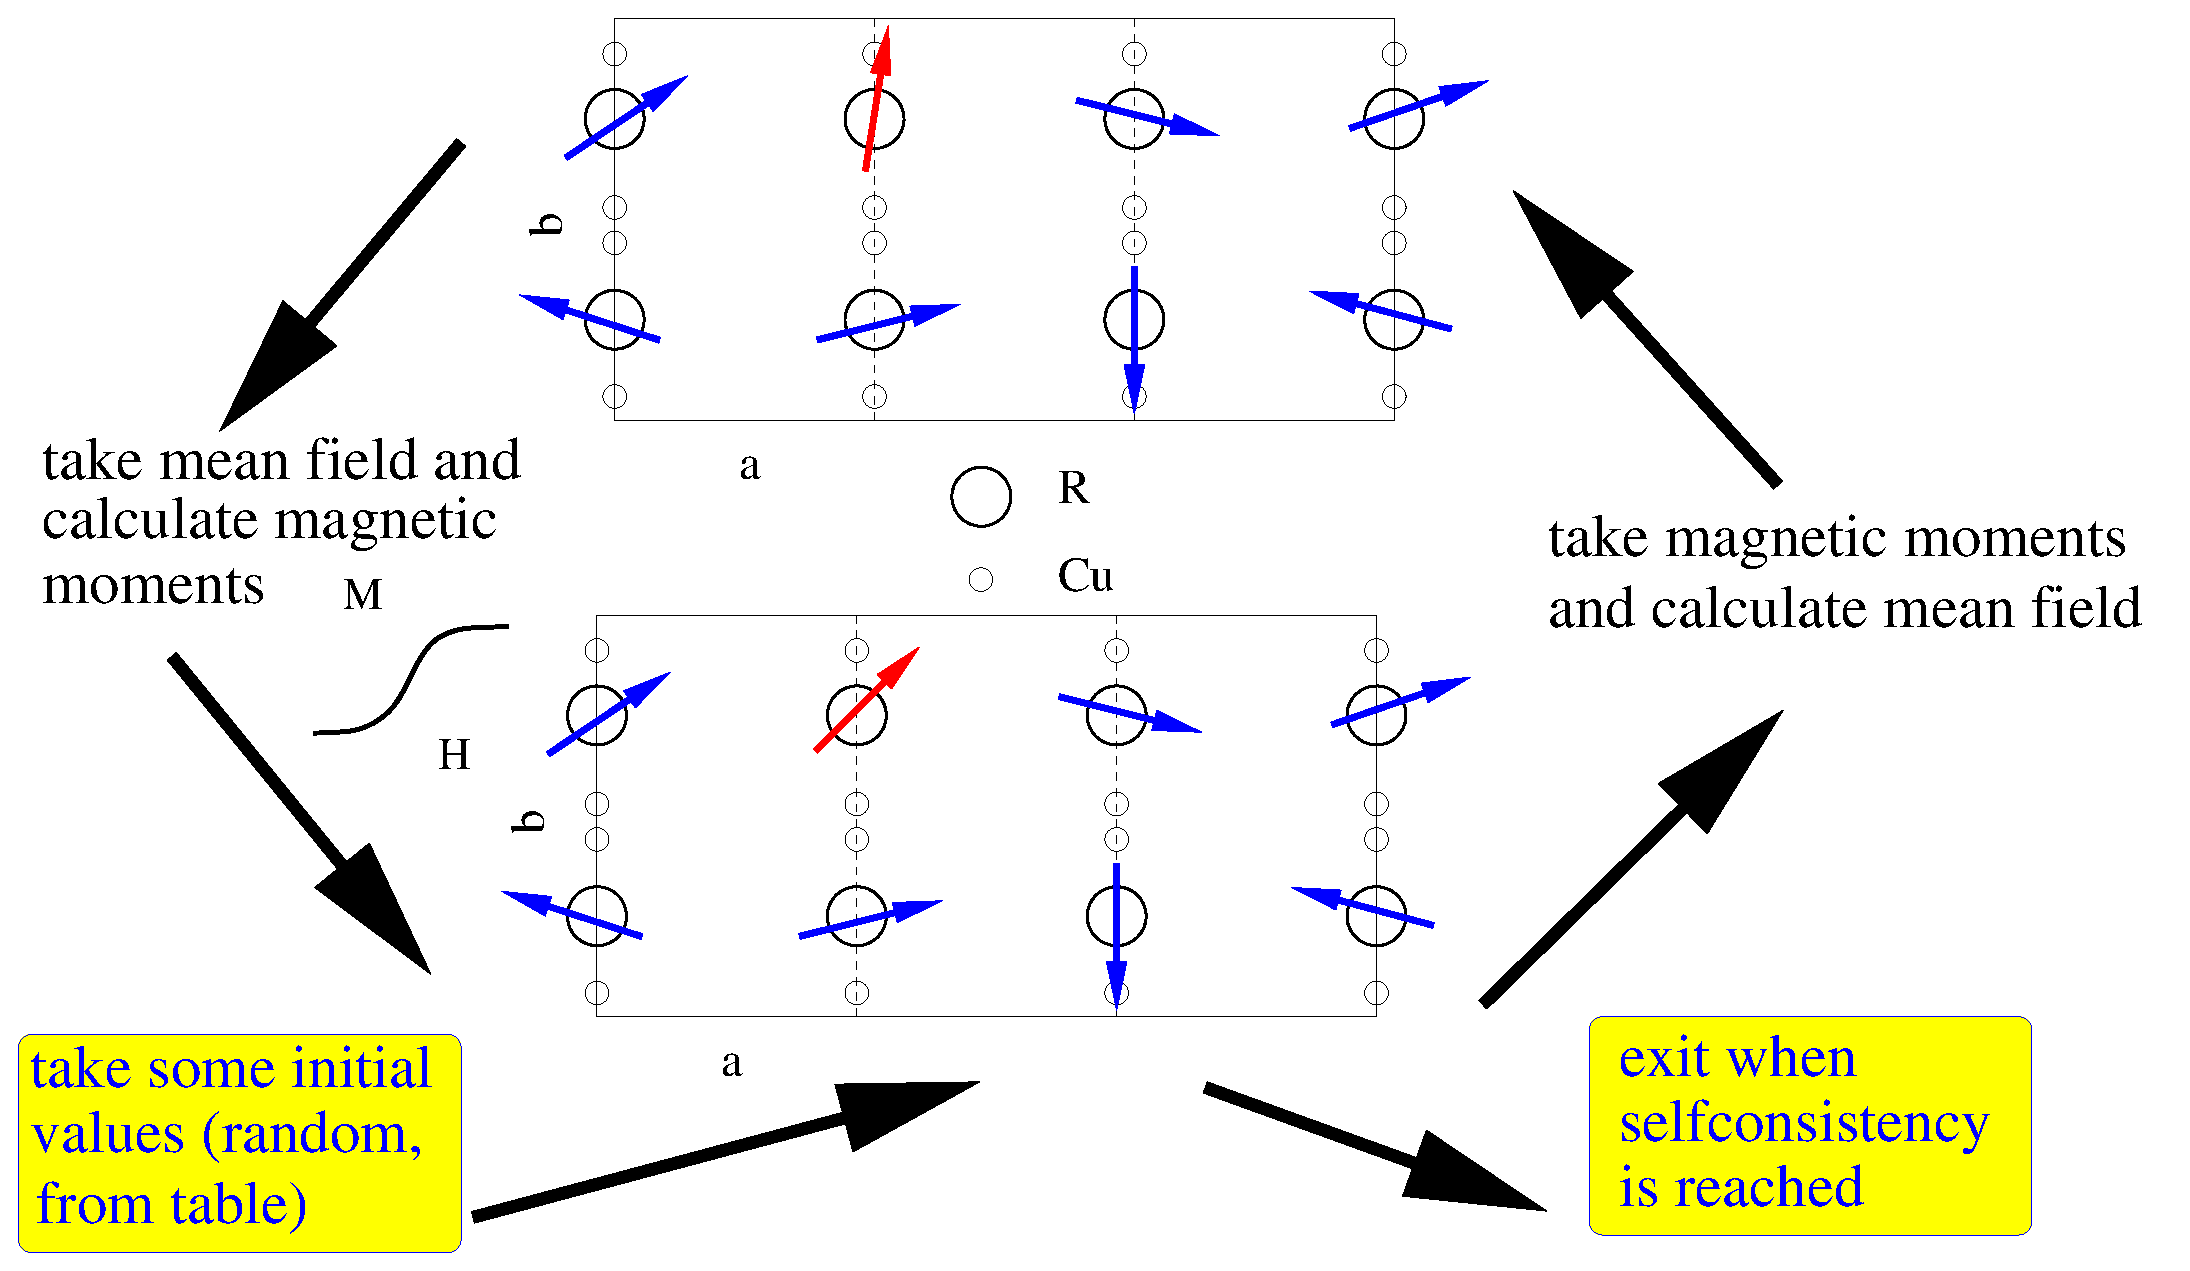
\includegraphics[angle=0,width=0.9\columnwidth]{figsrc/fecalc.eps}
\caption{\label{fecalc}Mean field process of sub {\prg fecalc}.}
\end{figure}

 
\subsubsection{Example {\prg mcphas.ini\index{mcphas.ini}} file for a simple antiferromagnet}

Here is an example of {\prg mcphas.ini\index{mcphas.ini}}, the comments describe the meaning of the different
parameters:

\input{mcphas.ini}



\subsubsection{{\prg mcphas.j\index{mcphas.j}} - lattice and exchange parameters}\label{mcphasj}
This file provides the information about 
the crystallographic
 structure and the magnetic exchange interactions.
For every atom in the crystallographic basis there
has to be given the coordinates, the number of neighbours to be considered, the 
Land\'e factor $g_J$, the single ion property filename and  a set of exchange parameters.
If the exchange parameters (and neighbour positions) are not known for your system, you 
can use the program module {\prg makenn\index{makenn}} (see section \ref{addprog}) to generate 
a list of nearest neighbours and
exchange parameters, currently implemented in {\prg makenn\index{makenn}} are dipolar interactions,
exchange interactions via the Bethe-Slater curve or the RKKY model. Note that in order
to use {\prg makenn\index{makenn}} you have to set up a working {\prg mcphas.j\index{mcphas.j}} file, which may or
may not contain neighbours and interactions.

Use program {\prg addj\index{addj}} to add exchange parameter set stored in different 
such {\prg .j} files (see section~\ref{addprog}).



\begin{description}
\item [Line 1,2:] Comment Lines
\item [Line 3:] lattice constants a,b,c and crystal angles alpha, beta, gamma 
\item [Line 4-6:] primitive lattice vectors
\item [Line 7:] Number of atoms in the primitive crystallographic unit cell ({\prg nofatoms})
\item [Line 8:] a comment line with stars
\item [Line 9:] coordinates  ($d_a$,$d_b$,$d_c$) of 1$^{st}$ magnetic ion in the crystallographic unit cell  with
respect to the lattice vectors $\vec a$,$\vec b$,$\vec c$. The number of neighbours of this 
ion, for which interaction constants are given in the interaction table (nofneighbours). 
If {\prg diagonalexchange}
is set to 0 the 9 components of the exchange tensor are given in column 4-12. 
If {\prg diagonalexchange}
 is 1, only 3 components are given (column 4-6).
If {\prg diagonalexchange}
 is 2, specific components of the exchange tensor can be given in columns 4 onwards. The indices of these components
 must be given in the following line (Line 9a below).
The Land\'e factor of the ion (gJ) and the file name of the corresponding single ion
parameter file (cffilename).
\item [Line 9a:]  If {\prg diagonalexchange=2}, then this line gives the indices of the exchange tensor corresponding to 
 the columns 4 onwards. It must have a variable called {\prg indexexchange} followed by a list of names of components of the interaction
 tensor separated by space. E.g.
 \verb|  #! indexexchange= JaJb JbJc  | 
means column 4 gives the the interaction constant between the
 first angular momentum component of the current ion with the second angular momentum component of its neighbour, whilst 
 column 5 has the interaction constant between the second angular momentum component of this ion with the third component of its
 neighbour. Alternatively, pairs of numbers may be given, as in \verb|  #! indexexchange= 1,2 2,3  |
 Additionally another parameter {\prg symmetricexchange} can be set to 1, where the value in each column is also used 
 for the transposed tensor component. Thus \verb|  #! symmetricexchange=1 indexexchange= JaJb  | is the same as \\
 \verb|  #! indexexchange= JaJb JbJa  | where the 4th and 5th column are the same.
\item [Line 10:]  Comment line
\item [Line 11-(10+nofneighbours):] Interaction table for ion number 1.   
Note: the neighbour coordinates (column 1-3) are given with respect to the lattice vectors
$\vec a$,$\vec b$,$\vec c$. The program then calculates from these values the coordinates
with respect to the primitive lattice $\vec r_1$,~$\vec r_2$,~$\vec r_3$.
($ d_a \vec a + d_b \vec b + d_c \vec c = d_1 \vec r_1 + d_2 \vec r_2 + d_3 \vec r_3$).
Column 4,5,6 \dots contain the components of the interaction tensor $\stackrel{=}{\mathcal J}$. 
Note that in case of non-orthogonal axes the 
components of the moments and the interaction tensor $Ja, Jb, Jc, Jaa, Jbb, Jcc, Jab ...$ 
refer to the orthogonal coordinate system
defined with respect to the nonorthogonal lattice $\vec a,\vec b,\vec c$ as
$Jb||\vec b$, $Jc||(\vec a \times \vec b)$ and $Ja$ perpendicular to $Jb$ and $Jc$.
\item [Line (11+nofneighbours) - end:] for each ion in the unit cell line 8 - (10+nofneighbours)
are repeated.
\end{description}


\vspace{0.5cm}

{\small {\bf Information for experienced users:}
\begin{description}
\item[\prg mcphas.jjj:]
format of exchange parameter file, which only needs a reduced set of exchange
parameters in the input file. Using the program {\prg jjj2j} the file can be transformed
to {\prg mcphas.j\index{mcphas.j}} by adding lines for all the equivalent neighbours. The format definition
of {\prg mcphas.jjj} is the same as {\prg mcphas.j\index{mcphas.j}}, however each line denotes several
equivalent neighbour atoms (instead of only one in {\prg mcphas.j\index{mcphas.j}}) according to the
 following rules:
\begin{itemize}
\item If a nonzero coordinate $d_a$ (or $d_b$,$d_c$) in the interaction table
 corresponds to it's value at the nearest
 lattice point of the primitive lattice,
  additional interactions of the same size
with  neighbours with coordinate $-d_a$ (or $-d_b$,$-d_c$, respectively)
are taken into account. This
holds for each of the three coordinates $d_a$,$d_b$ and $d_c$
 resulting in a maximum
number of 8 equivalent neighbours per line in the interaction table.
\item If the value of $d_a$ (or $d_b$,$d_c$) is zero or differs
from it's value at the nearest lattice point of the primitive lattice, it is 
changed to the value at the nearest lattice point and {\bf no} interaction 
with  neighbours with coordinates $-d_a$ (or $-d_b$,$-d_c$) is
 taken into account. If such
 interaction is needed it may be given in a different line and may
have different magnitude. In this way also crystallographic lattices
with no mirror symmetry may be described.
\end{itemize}
\item[\prg mcphas.coq:]   exchange parameters etc [ in old format]...see examples for details, use {\prg coq2jjj} to 
transform {\prg mcphas.coq} to {\prg mcphas.jjj} format
\end{description}

}


\subsubsection{Example {\prg mcphas.j\index{mcphas.j}} file for a simple antiferromagnet}

Here are example files of a tetragonal antiferromagnet with nearest neighbour interactions, all
files are equivalent:

{\small
\begin{verbatim} 
# simple antiferromagnet 
#<!--mcphase.mcphas.j-->
#***************************************************************
# Lattice Constants (A)
#! a=4.3843 b=4.3843 c=2.4194 alpha=  90 beta=  90 gamma=  90
#! r1a=   1 r2a=   0 r3a=   0
#! r1b=   0 r2b=   1 r3b=   0   primitive lattice vectors [a][b][c]
#! r1c=   0 r2c=   0 r3c=   1
#! nofatoms=1  nofcomponents=3  number of atoms in primitive unit cell/number of components of each spin
# ****************************************************************************
#! da=  0 [a] db=  0 [b] dc=  0 nofneighbours=2 diagonalexchange=0 gJ=0.857143 cffilename=Ce3p.sipf
# da[a] db[b] dc[c] Jaa[meV] Jbb[meV] Jcc[meV] Jab[meV] Jba[meV] Jac[meV] Jca[meV] Jbc[meV] Jcb[meV]
+0	+0	+1	-0.1	-0.1	-0.1   0  0  0  0  0  0
+0	+0	-1	-0.1	-0.1	-0.1   0  0  0  0  0  0
#\end{verbatim}
}

Using diagonalexchange this may be shortened to

{\small
\begin{verbatim} 
# simple antiferromagnet 
#<!--mcphase.mcphas.j-->
#***************************************************************
# Lattice Constants (A)
#! a=4.3843 b=4.3843 c=2.4194 alpha=  90 beta=  90 gamma=  90
#! r1a=   1 r2a=   0 r3a=   0
#! r1b=   0 r2b=   1 r3b=   0   primitive lattice vectors [a][b][c]
#! r1c=   0 r2c=   0 r3c=   1
#! nofatoms=1  nofcomponents=3  number of atoms in primitive unit cell/number of components of each spin
# ****************************************************************************
#! da=  0 [a] db=  0 [b] dc=  0 nofneighbours=2 diagonalexchange=1 gJ=0.857143 cffilename=Ce3p.sipf
# da[a] db[b] dc[c] Jaa[meV] Jbb[meV] Jcc[meV] Jab[meV] Jba[meV] Jac[meV] Jca[meV] Jbc[meV] Jcb[meV]
+0	+0	+1	-0.1	-0.1	-0.1   
+0	+0	-1	-0.1	-0.1	-0.1   
#\end{verbatim}
}

with indexexchange option the sequence of two ion interaction parameters can be changed and
zero parameters may be omitted:

{\small
\begin{verbatim} 
# simple antiferromagnet 
#<!--mcphase.mcphas.j-->
#***************************************************************
# Lattice Constants (A)
#! a=4.3843 b=4.3843 c=2.4194 alpha=  90 beta=  90 gamma=  90
#! r1a=   1 r2a=   0 r3a=   0
#! r1b=   0 r2b=   1 r3b=   0   primitive lattice vectors [a][b][c]
#! r1c=   0 r2c=   0 r3c=   1
#! nofatoms=1  nofcomponents=3  number of atoms in primitive unit cell/number of components of each spin
# ****************************************************************************
#! da=  0 [a] db=  0 [b] dc=  0 nofneighbours=2 diagonalexchange=2 gJ=0.857143 cffilename=Ce3p.sipf
# da[a] db[b] dc[c] Jaa[meV] Jbb[meV] Jcc[meV] Jab[meV] Jba[meV] Jac[meV] Jca[meV] Jbc[meV] Jcb[meV]
#! indexexchange = JaJa JaJc JcJa JbJb JcJc
+0	+0	+1	-0.1 0 0 -0.1	-0.1  
+0	+0	-1	-0.1 0 0 -0.1	-0.1  
#\end{verbatim}
}

{\small
\begin{verbatim} 
# simple antiferromagnet 
#<!--mcphase.mcphas.j-->
#***************************************************************
# Lattice Constants (A)
#! a=4.3843 b=4.3843 c=2.4194 alpha=  90 beta=  90 gamma=  90
#! r1a=   1 r2a=   0 r3a=   0
#! r1b=   0 r2b=   1 r3b=   0   primitive lattice vectors [a][b][c]
#! r1c=   0 r2c=   0 r3c=   1
#! nofatoms=1  nofcomponents=3  number of atoms in primitive unit cell/number of components of each spin
# ****************************************************************************
#! da=  0 [a] db=  0 [b] dc=  0 nofneighbours=2 diagonalexchange=2 gJ=0.857143 cffilename=Ce3p.sipf
# da[a] db[b] dc[c] Jaa[meV] Jbb[meV] Jcc[meV] Jab[meV] Jba[meV] Jac[meV] Jca[meV] Jbc[meV] Jcb[meV]
#! indexexchange = 1,1 1,3, 3,1 2,2 3,3
+0	+0	+1	-0.1 0 0 -0.1	-0.1  
+0	+0	-1	-0.1 0 0 -0.1	-0.1  
#\end{verbatim}
}


using symmetricexchange together with indexexchange will assume that the interaction tensor is symmetic and 
only half of it may be given:

{\small
\begin{verbatim} 
# simple antiferromagnet 
#<!--mcphase.mcphas.j-->
#***************************************************************
# Lattice Constants (A)
#! a=4.3843 b=4.3843 c=2.4194 alpha=  90 beta=  90 gamma=  90
#! r1a=   1 r2a=   0 r3a=   0
#! r1b=   0 r2b=   1 r3b=   0   primitive lattice vectors [a][b][c]
#! r1c=   0 r2c=   0 r3c=   1
#! nofatoms=1  nofcomponents=3  number of atoms in primitive unit cell/number of components of each spin
# ****************************************************************************
#! da=  0 [a] db=  0 [b] dc=  0 nofneighbours=2 diagonalexchange=2 gJ=0.857143 cffilename=Ce3p.sipf
# da[a] db[b] dc[c] Jaa[meV] Jbb[meV] Jcc[meV] Jab[meV] Jba[meV] Jac[meV] Jca[meV] Jbc[meV] Jcb[meV]
#! symmetricexchange=1 indexexchange = JaJa JaJc JbJb JcJc
+0	+0	+1	-0.1 0  -0.1	-0.1  
+0	+0	-1	-0.1 0  -0.1	-0.1  
#\end{verbatim}
}


\subsubsection{Single Ion Property Input Files}\label{sifile}

In order to speed up calculations or treat special problems a large 
variety of single ion modules is available. This includes the
option to load a user written single ion module. Details are 
given in chapter~\ref{simod}.

The first time user of {\prg McPhase} should use the module {\prg so1ion}\index{so1ion} and 
create an appropriate single ion property input file as described in
section \ref{cf1ion}. A good starting point are several examples
given in directory {\prg examples}.


\subsubsection{Example single ion property file  for a simple antiferromagnet}

Here is an example file {\prg mcphas.cf1} describing the anisotropy of a 
simple antiferromagnet with Ce atoms having basal plane anisotropy. Note the
axis convention xyz$||$abc, in case of non-orthogonal axes the convention 
is $y||\vec b$, $z||(\vec a \times \vec b)$ and $x$ perpendicular to $y$ and $z$.


\input{mcphas.cf1}

\subsubsection{{\prg mcphas.tst\index{mcphas.tst}} - input file of test spin-configurations (optional)}
This file is optional and contains
some test momentum configurations to be used for the calculation
             of the free energy. Mind that
\begin{itemize}
\item  in the file header the number of atoms in the primitive
       crystallographic unit cell and the number of components
       of the spin vector have to be given.
\item  at the end of the
 file there must be no empty lines !
\end{itemize}

The momentum - configurations tables always refer to spins sitting on
the primitive lattice ${\mbf r}_i$. If more than one atom is in
the primitive basis, the momentum gets $3n$ components ($n=$ number
of atoms in the crystallographic basis). See {\prg ./examples/ndcu2b\_new/} for
examples of a two atom basis. Units of these tables are that of total 
angular momentum $<J>$.

\subsubsection{Example {\prg mcphas.tst\index{mcphas.tst}} file  for a simple antiferromagnet}

Here is the file {\prg mcphas.tst\index{mcphas.tst}} for the simple antiferromagnet example
describing some spin configurations
to be used as starting values for the mean field process:

\input{mcphas.tst}
Note, in case of non-orthogonal axes the convention 
is $mb||\vec b$, $mc||(\vec a \times \vec b)$ and $ma$ perpendicular to $mb$ and $mc$.

\subsubsection{subdirectory {\prg ./results} - directory where calculated data is stored}

In order to be able to save the results of a calculation the directory {\prg ./results} has to
exist. Mind that all files in this directory will be overwritten without warning. 

\subsubsection{subdirectory {\prg ./fit} - experimental data for fit (optional) } 

In order that {\prg McPhase} can calculate the standard deviation between
 experimental data and the results of the simulation, some experimental data
 can be given in the subdirectory {\prg ./fit}. The filenames and the data-format
 are the same as the output files of {\prg McPhas}, e.g. {\prg mcphas.fum}, {\prg mcphas.hkl}
 etc. {\prg McPhase} looks into the directory {\prg ./fit} and if it finds any
 of these files, the standard deviation is increased correspondingly. 

What measurement data can be used to calculate a standard deviation ?

\begin{description}
\item[{\prg mcphas.fum}] if given in column 11, 12, 13 in {\prg ./fit/mcphas.fum} the
            magnetisation in the $a$, $b$ and $c$ direction is used for calculation
	    of the standard deviation sta. The standard deviation is calculated
	    as ${\rm sta}=\sum_{\rm data points i} ({\mbf m}_i^{calc}-{\mbf m}_i^{meas})^2$.
	    All three components of the magnetic moment have to be given and are used.

\end{description}

Note that the measured data has to be given in those (H-T) points which are 
calculated by mcphas\index{mcphas} in order to be used by the program to increase {\prg sta}.
It is usually most effective to fit only few data points, because a large set
of data points will not improve the quality of the fit and only require a large
amount of calculation time.



\subsection{Starting a simulation}
\label{start}

To start the simulation goto the directory containing the
input files {\prg mcphas.ini, mcphas.j, etc. } and type

\begin{description}
\item[\prg mcphas] to run the program generating stepwise $H-T$ values 
              in a loop given by {\prg mcphas.ini\index{mcphas.ini}} (you can also press the
              symbol in the {\prg McPhase - Explorer} window).
\item[\prg mcphas\index{mcphas} [file]]  to run the program with an input file --   
             {\prg file} contains T ha hb hc values to be calculated 
             if [file] is not given, xmin xmax xstep (xT xHa xHb xHc)
             ymin ymax ystep (yT yHa yHb yHc) is read from file {\prg mcphas.ini\index{mcphas.ini}}
	     and phase diagram is calculated
\item[\prg mcphas\index{mcphas} -h]  to  print help and version of {\prg McPhas}.
\item[\prg mcphas\index{mcphas} -stamax 14]  end mcphas\index{mcphas} if standard deviation exceeds 14.
\item[\prg mcphas\index{mcphas} -a] avoid overwriting output files in results, append new results to existing files
\item[\prg mcphas\index{mcphas} -v]  to  enable verbose mode with lots of messages of {\prg McPhas}. Specifically
the verbose mode enables the following features:
  \begin{itemize}
			          \item more information is printed out, 
			          \item the q-vectors file {\prg ./results/mcphas.qvc} will contain 
				    the explicit spin configurations
			          \item the display\index{display} on screen (ghostview window using 
				     {\prg ./results/.sps.eps}) will be updated not only 
				    when a H-T point has been finished but always 
				    when a structure with smaller free energy 
				    has been stabilised
  \end{itemize}
\item[\prg mcphasit\index{mcphas}] to start mcphase in commandline mode without opening any window
\end{description}

\vspace{1cm}
{\em Exercises:}
\begin{itemize}
\item Look at the input files for {\prg McPhase} given in the directory
{\prg examples/ndcu2b\_new}.  How many atoms are contained in the crystallographic basis ?
\item
Start the simulation by typing the command {\prg mcphas}.
\end{itemize}



\subsection{Options for a running simulation}
... when the program is running, the options in the main window
can be changed. Pressing ''displayall'' displays the current spin-configuration
at each iteration step. Pressing ''log fe vs Q'' appends free energy vs Q
data to {\prg mcphas.log} for every ($T-H$) point.


The file {\prg ./results/.spins.eps} is used to show the information about the currently calculated
spin structure on the screen using the postscript file viewer ghostview.

The file {\prg ./results/.mcphas.fum} contains the information of the magnetisation curve
which is currently calculated. This information is automatically displayed on the screen.


The program {\prg display} (see section \ref{display}) can be used 
for the online display\index{display} of any other
curve(s).


\subsection{Output Files - {\prg mcphas.qvc,phs,sps,mf,fum,j1...,xyt,hkl} }\label{outputfiles}
 (in directory ./results/ after a simulation run) 

\begin{figure}[htb]%h=here, t=top, b=bottom, p=separate figure page
\begin{center}\leavevmode
\includegraphics[angle=0, width=0.3\textwidth]{figsrc/magnetization_ndcu2.ps}
\end{center}
\caption{Calculated magnetisation of NdCu$_2$ for field parallel to the orthorhombic $b$-direction.}
\label{magnetization}
\end{figure}

\begin{figure}[htb]%h=here, t=top, b=bottom, p=separate figure page
\begin{center}\leavevmode
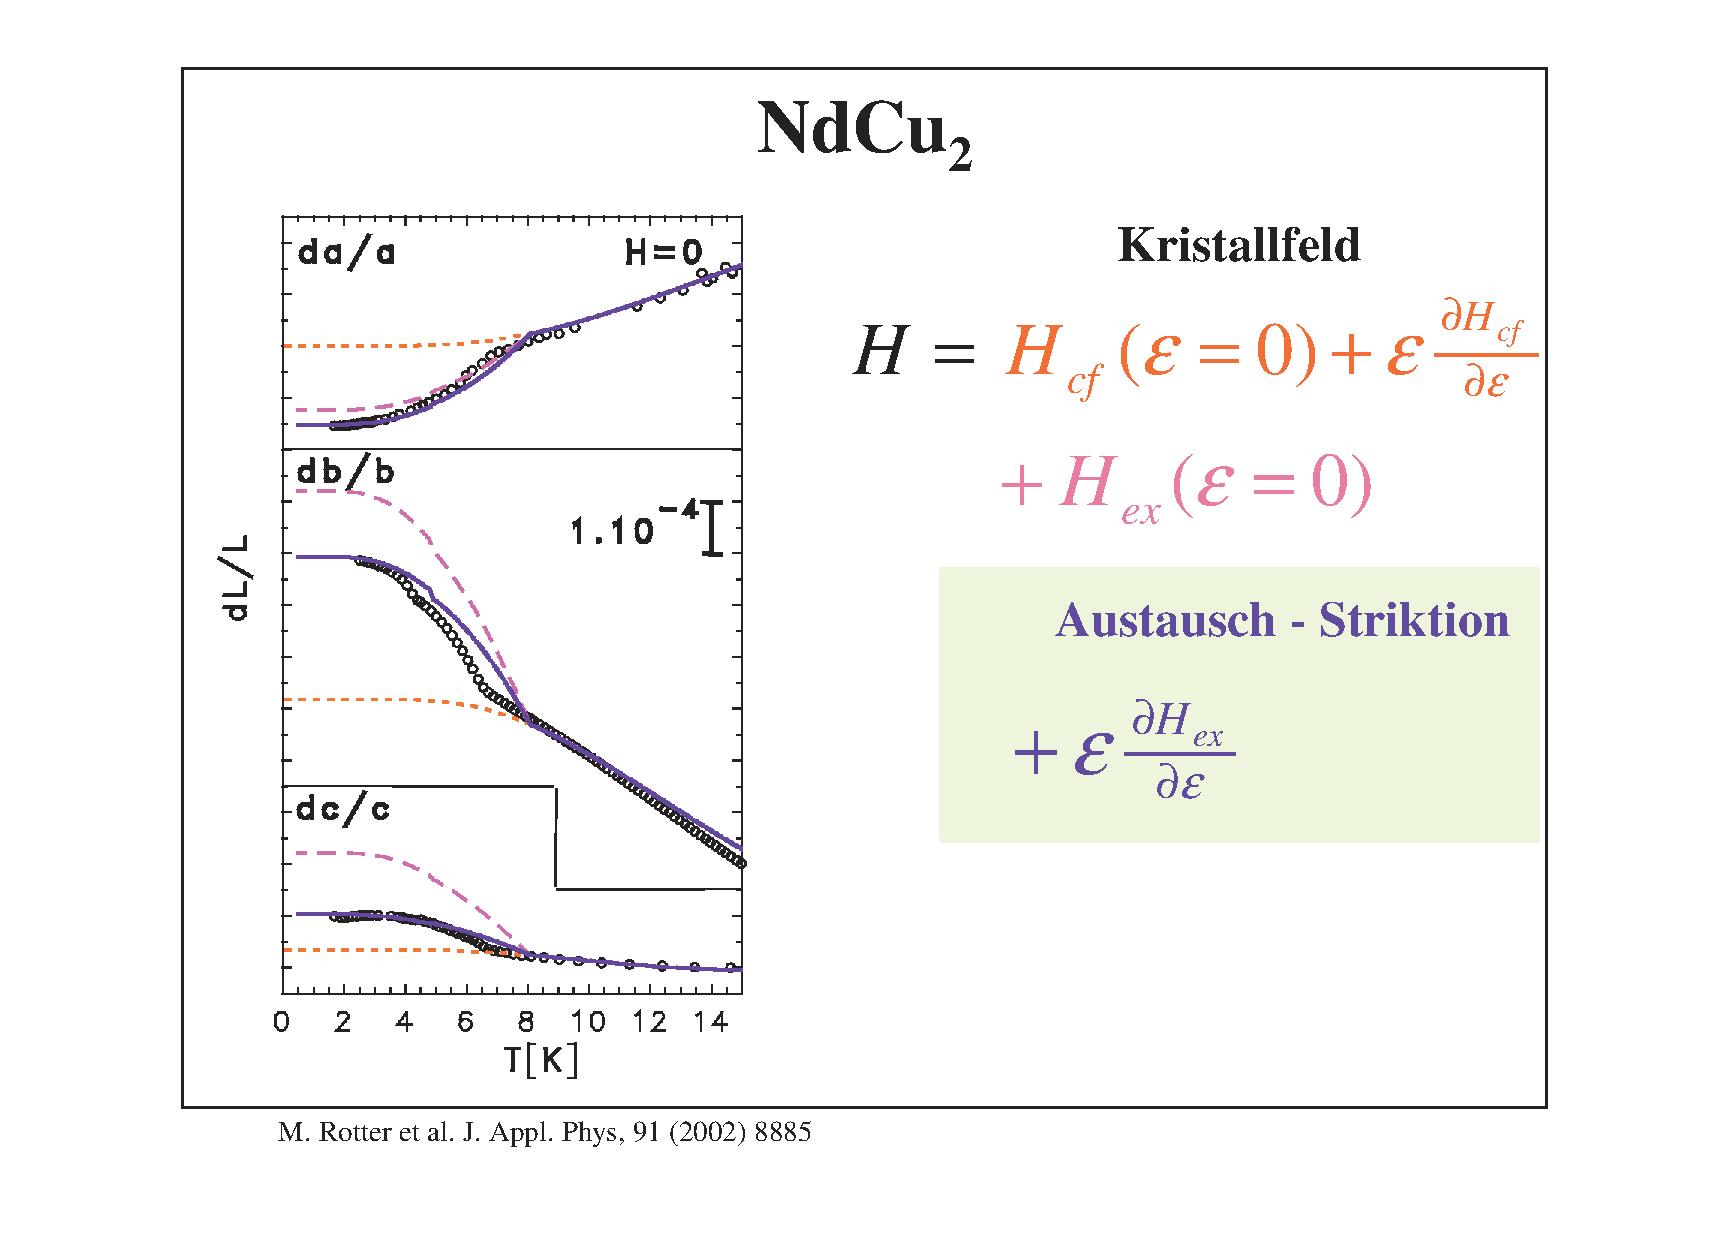
\includegraphics[angle=0, width=0.8\textwidth]{figsrc/magnetostriction_ndcu2.eps}
\end{center}
\caption{Calculated spontaneous magnetostriction of NdCu$_2$.}
\label{magnetostrictiongraphic}
\end{figure}

\begin{description}
\item [\prg mcphas.qvc]    the set of test q-vectors used for calculation of free energy.
                           Components of these q vectors refer to the reciprocal lattice $\vec a^*,\vec b^*,\vec c^*$.
\item [\prg mcphas.phs]    spin-configuration table of different types of spin-configurations. 
                            Note, in case of non-orthogonal axes the convention in these tables 
                            is $mb||\vec b$, $mc||(\vec a \times \vec b)$ and $ma$ perpendicular to $mb$ and $mc$.

                           {\em Note}: 
                           there is no natural criteria for deciding, if one spin-configuration is
			   different from another one. Therefore the list of ''different''
			   spin-configurations is dependent on the meaning of ''different''.
			   
			   The program {\prg McPhase} decides whether a spin-configuration is
			   different from another by a simple criteria, namely by the
			   angle between the spins. Comparing two spin configurations it calculates
			   the angle between corresponding spins and if for one spin the
			   angle is not small, the configuration is treated as a different
			   configuration. Therefore for example a ferromagnet with moments
			   in $a$ has a different spin configuration than a ferromagnet with
			   moments in $b$ direction. 
\item [\prg mcphas.sps]    $T-H$ dependence of spin-configuration. The spin configurations stored in this
                           file may be displayed using the program {\prg spins\index{spins}}, an example is given
			   in figure~\ref{spingraphic}.
                            Note, in case of non-orthogonal axes the convention for applied field $Ha, Hb,Hc$ and
                            also for the moment components $ma, mb, mc$ in these tables 
                            is $mb||\vec b$, $mc||(\vec a \times \vec b)$ and $ma$ perpendicular to $mb$ and $mc$.

\item [\prg mcphas.mf]     $T-H$ dependence of exchange field configuration, stored as $g_J \mu_B H_{xc}(i)$(unit is in meV)
                            for i=1,2,...,number of spins in magnetic unit cell.
                            Note, in case of non-orthogonal axes the convention for applied field $Ha, Hb,Hc$ and
                            also for the mean field components in these tables 
                            is $Hb||\vec b$, $Hc||(\vec a \times \vec b)$ and $Ha$ perpendicular to $Hb$ and $Hc$.
\item [\prg mcphas.fum]    free energy, magnetic energy (the derivative with respect to temperature gives the specific %%@
heat),
                           magnetisation data and (if cfield is used with higher order interactions)
                           expectation values of the Stevens Operators $<O_l^m>$ . As an example for the information
			   contained in this file the calculated magnetisation and magnetostriction of NdCu$_2$ is shown in
			   figures~\ref{magnetization} and ~\ref{magnetizationgraphic}.
                            Note, in case of non-orthogonal axes the convention for applied field $Ha, Hb,Hc$ and
                            also for the magnetisation components $ma,mb,mc$ in these tables 
                            is $Hb||\vec b$, $Hc||(\vec a \times \vec b)$ and $Ha$ perpendicular to $Hb$ and $Hc$.

\item [\prg mcphas1.j1 .j1 .j2 ...] 
               spin-spin correlation functions for sub-lattice 1 neighbour 1 2 ...
	       (linear combination is proportional to magnetostriction)
	       The spin-spin correlation functions for neighbour $k$ are defined by
	       the following sum of dyadic products:

	       \begin{equation}
	        \frac{1}{n}\sum_{s=1}^n <{\mbf J}^s> \times  <{\mbf J}^{s+k}>
	       \end{equation}
	       with $n$ being the number of moments in the magnetic unit cell.
	       Single ion and two-ion magnetostriction can be calculated using the $<O_l^m>$ and the
	       spin-spin correlation functions. As an example the magnetostriction analysis of
	       NdCu$_2$ is shown in figure~\ref{magnetostrictiongraphic}. For details 
             please refer to~\cite{rotter02-8885}.
                            Note, in case of non-orthogonal axes the convention for applied field $Ha, Hb,Hc$ and
                            also for the moment components in these tables 
                            is $Hb||\vec b$, $Hc||(\vec a \times \vec b)$ and $Ha$ perpendicular to $Hb$ and $Hc$.
\item [\prg mcphas.xyt]    phase diagram as x,y,T, H, phase-number j according to spin-configuration table
               given in mcphas.phs, a periodicity key, nettomoments <J>.
 Figure~\ref{phasediagramgraphic}
	       shows the phase diagram of NdCu$_2$ for magnetic fields parallel to the orthorhombic $b$-direction.
                            Note, in case of non-orthogonal axes the convention for applied field $Ha, Hb,Hc$ 
                             in these tables 
                            is $Hb||\vec b$, $Hc||(\vec a \times \vec b)$ and $Ha$ perpendicular to $Hb$ and $Hc$.
\item [\prg mcphas.hkl]    calculated (unpolarised) neutron diffraction data (the calculated magnetic intensities
    correspond to the magnetic structure + Polarisation factor. The
    Lorentz-factor , magnetic form factor and  instrumental corrections are not calculated.)
 As an example figure~\ref{neutintgraphic}
    shows the calculated temperature dependence of magnetic amplitudes for NdCu$_2$.
                           $h,k,l$ refer to the reciprocal lattice $\vec a^*,\vec b^*,\vec c^*$.
                            Note, in case of non-orthogonal axes the convention for applied field $Ha, Hb,Hc$ 
                             in these tables 
                            is $Hb||\vec b$, $Hc||(\vec a \times \vec b)$ and $Ha$ perpendicular to $Hb$ and $Hc$.
    
\item [\prg mcphasa.hkl]    Fourier Transform of the $a$-component of the magnetic Moments.
                           $h,k,l$ refer to the reciprocal lattice $\vec a^*,\vec b^*,\vec c^*$.
                            Note, in case of non-orthogonal axes the convention for applied field $Ha, Hb,Hc$ and
                            the magnetic moment component in these tables 
                            is $Hb||\vec b$, $Hc||(\vec a \times \vec b)$ and $Ha$ perpendicular to $Hb$ and $Hc$.
\item [\prg mcphasb.hkl]    Fourier Transform of the $b$-component of the magnetic Moments.
                           $h,k,l$ refer to the reciprocal lattice $\vec a^*,\vec b^*,\vec c^*$.
                            Note, in case of non-orthogonal axes the convention for applied field $Ha, Hb,Hc$ and
                            the magnetic moment component in these tables 
                            is $Hb||\vec b$, $Hc||(\vec a \times \vec b)$ and $Ha$ perpendicular to $Hb$ and $Hc$.
\item [\prg mcphasc.hkl]    Fourier Transform of the $c$-component of the magnetic Moments.
                           $h,k,l$ refer to the reciprocal lattice $\vec a^*,\vec b^*,\vec c^*$.
                            Note, in case of non-orthogonal axes the convention for applied field $Ha, Hb,Hc$ and
                            the magnetic moment component in these tables 
                            is $Hb||\vec b$, $Hc||(\vec a \times \vec b)$ and $Ha$ perpendicular to $Hb$ and $Hc$.
\end{description} 

\vspace{1cm}
{\em Exercises:}
\begin{itemize}
\item Look at the output files of {\prg McPhase}  in the directory
{\prg examples/ndcu2b\_new/results}.  At which magnetic field
the ferromagnetically aligned state is achieved (at $T=$2~K)?
\item
What is the propagation vector in the different antiferromagnetic phases at $T=$2~K ?
\end{itemize}





\subsubsection{{\prg mcphas.j\index{mcphas.j}} - lattice and exchange parameters}\label{mcphasj}
This file provides the information about 
the crystallographic
 structure and the magnetic exchange interactions.
For every atom in the crystallographic basis there
has to be given the coordinates, the number of neighbours to be considered, the 
Land\'e factor $g_J$, the single ion property filename and  a set of exchange parameters.
If the exchange parameters (and neighbour positions) are not known for your system, you 
can use the program module {\prg makenn\index{makenn}} (see section \ref{addprog}) to generate 
a list of nearest neighbours and
exchange parameters, currently implemented in {\prg makenn\index{makenn}} are dipolar interactions,
exchange interactions via the Bethe-Slater curve or the RKKY model. Note that in order
to use {\prg makenn\index{makenn}} you have to set up a working {\prg mcphas.j\index{mcphas.j}} file, which may or
may not contain neighbours and interactions.

Use program {\prg addj\index{addj}} to add exchange parameter set stored in different 
such {\prg .j} files (see section~\ref{addprog}).



\begin{description}
\item [Line 1,2:] Comment Lines
\item [Line 3:] lattice constants a,b,c and crystal angles alpha, beta, gamma 
\item [Line 4-6:] primitive lattice vectors
\item [Line 7:] Number of atoms in the primitive crystallographic unit cell ({\prg nofatoms})
\item [Line 8:] a comment line with stars
\item [Line 9:] coordinates  ($d_a$,$d_b$,$d_c$) of 1$^{st}$ magnetic ion in the crystallographic unit cell  with
respect to the lattice vectors $\vec a$,$\vec b$,$\vec c$. The number of neighbours of this 
ion, for which interaction constants are given in the interaction table (nofneighbours). 
If {\prg diagonalexchange}
is set to 0 the 9 components of the exchange tensor are given in column 4-12. 
If {\prg diagonalexchange}
 is 1, only 3 components are given (column 4-6).
If {\prg diagonalexchange}
 is 2, specific components of the exchange tensor can be given in columns 4 onwards. The indices of these components
 must be given in the following line (Line 9a below).
The Land\'e factor of the ion (gJ) and the file name of the corresponding single ion
parameter file (cffilename).
\item [Line 9a:]  If {\prg diagonalexchange=2}, then this line gives the indices of the exchange tensor corresponding to 
 the columns 4 onwards. It must have a variable called {\prg indexexchange} followed by a list of names of components of the interaction
 tensor separated by space. E.g.
 \verb|  #! indexexchange= JaJb JbJc  | 
means column 4 gives the the interaction constant between the
 first angular momentum component of the current ion with the second angular momentum component of its neighbour, whilst 
 column 5 has the interaction constant between the second angular momentum component of this ion with the third component of its
 neighbour. Alternatively, pairs of numbers may be given, as in \verb|  #! indexexchange= 1,2 2,3  |
 Additionally another parameter {\prg symmetricexchange} can be set to 1, where the value in each column is also used 
 for the transposed tensor component. Thus \verb|  #! symmetricexchange=1 indexexchange= JaJb  | is the same as \\
 \verb|  #! indexexchange= JaJb JbJa  | where the 4th and 5th column are the same.
\item [Line 10:]  Comment line
\item [Line 11-(10+nofneighbours):] Interaction table for ion number 1.   
Note: the neighbour coordinates (column 1-3) are given with respect to the lattice vectors
$\vec a$,$\vec b$,$\vec c$. The program then calculates from these values the coordinates
with respect to the primitive lattice $\vec r_1$,~$\vec r_2$,~$\vec r_3$.
($ d_a \vec a + d_b \vec b + d_c \vec c = d_1 \vec r_1 + d_2 \vec r_2 + d_3 \vec r_3$).
Column 4,5,6 \dots contain the components of the interaction tensor $\stackrel{=}{\mathcal J}$. 
Note that in case of non-orthogonal axes the 
components of the moments and the interaction tensor $Ja, Jb, Jc, Jaa, Jbb, Jcc, Jab ...$ 
refer to the orthogonal coordinate system
defined with respect to the nonorthogonal lattice $\vec a,\vec b,\vec c$ as
$Jb||\vec b$, $Jc||(\vec a \times \vec b)$ and $Ja$ perpendicular to $Jb$ and $Jc$.
\item [Line (11+nofneighbours) - end:] for each ion in the unit cell line 8 - (10+nofneighbours)
are repeated.
\end{description}


\vspace{0.5cm}

{\small {\bf Information for experienced users:}
\begin{description}
\item[\prg mcphas.jjj:]
format of exchange parameter file, which only needs a reduced set of exchange
parameters in the input file. Using the program {\prg jjj2j} the file can be transformed
to {\prg mcphas.j\index{mcphas.j}} by adding lines for all the equivalent neighbours. The format definition
of {\prg mcphas.jjj} is the same as {\prg mcphas.j\index{mcphas.j}}, however each line denotes several
equivalent neighbour atoms (instead of only one in {\prg mcphas.j\index{mcphas.j}}) according to the
 following rules:
\begin{itemize}
\item If a nonzero coordinate $d_a$ (or $d_b$,$d_c$) in the interaction table
 corresponds to it's value at the nearest
 lattice point of the primitive lattice,
  additional interactions of the same size
with  neighbours with coordinate $-d_a$ (or $-d_b$,$-d_c$, respectively)
are taken into account. This
holds for each of the three coordinates $d_a$,$d_b$ and $d_c$
 resulting in a maximum
number of 8 equivalent neighbours per line in the interaction table.
\item If the value of $d_a$ (or $d_b$,$d_c$) is zero or differs
from it's value at the nearest lattice point of the primitive lattice, it is 
changed to the value at the nearest lattice point and {\bf no} interaction 
with  neighbours with coordinates $-d_a$ (or $-d_b$,$-d_c$) is
 taken into account. If such
 interaction is needed it may be given in a different line and may
have different magnitude. In this way also crystallographic lattices
with no mirror symmetry may be described.
\end{itemize}
\item[\prg mcphas.coq:]   exchange parameters etc [ in old format]...see examples for details, use {\prg coq2jjj} to 
transform {\prg mcphas.coq} to {\prg mcphas.jjj} format
\end{description}

}


\subsubsection{Example {\prg mcphas.j\index{mcphas.j}} file for a simple antiferromagnet}

Here are example files of a tetragonal antiferromagnet with nearest neighbour interactions, all
files are equivalent:

{\small
\begin{verbatim} 
# simple antiferromagnet 
#<!--mcphase.mcphas.j-->
#***************************************************************
# Lattice Constants (A)
#! a=4.3843 b=4.3843 c=2.4194 alpha=  90 beta=  90 gamma=  90
#! r1a=   1 r2a=   0 r3a=   0
#! r1b=   0 r2b=   1 r3b=   0   primitive lattice vectors [a][b][c]
#! r1c=   0 r2c=   0 r3c=   1
#! nofatoms=1  nofcomponents=3  number of atoms in primitive unit cell/number of components of each spin
# ****************************************************************************
#! da=  0 [a] db=  0 [b] dc=  0 nofneighbours=2 diagonalexchange=0 gJ=0.857143 cffilename=Ce3p.sipf
# da[a] db[b] dc[c] Jaa[meV] Jbb[meV] Jcc[meV] Jab[meV] Jba[meV] Jac[meV] Jca[meV] Jbc[meV] Jcb[meV]
+0	+0	+1	-0.1	-0.1	-0.1   0  0  0  0  0  0
+0	+0	-1	-0.1	-0.1	-0.1   0  0  0  0  0  0
#\end{verbatim}
}

Using diagonalexchange this may be shortened to

{\small
\begin{verbatim} 
# simple antiferromagnet 
#<!--mcphase.mcphas.j-->
#***************************************************************
# Lattice Constants (A)
#! a=4.3843 b=4.3843 c=2.4194 alpha=  90 beta=  90 gamma=  90
#! r1a=   1 r2a=   0 r3a=   0
#! r1b=   0 r2b=   1 r3b=   0   primitive lattice vectors [a][b][c]
#! r1c=   0 r2c=   0 r3c=   1
#! nofatoms=1  nofcomponents=3  number of atoms in primitive unit cell/number of components of each spin
# ****************************************************************************
#! da=  0 [a] db=  0 [b] dc=  0 nofneighbours=2 diagonalexchange=1 gJ=0.857143 cffilename=Ce3p.sipf
# da[a] db[b] dc[c] Jaa[meV] Jbb[meV] Jcc[meV] Jab[meV] Jba[meV] Jac[meV] Jca[meV] Jbc[meV] Jcb[meV]
+0	+0	+1	-0.1	-0.1	-0.1   
+0	+0	-1	-0.1	-0.1	-0.1   
#\end{verbatim}
}

with indexexchange option the sequence of two ion interaction parameters can be changed and
zero parameters may be omitted:

{\small
\begin{verbatim} 
# simple antiferromagnet 
#<!--mcphase.mcphas.j-->
#***************************************************************
# Lattice Constants (A)
#! a=4.3843 b=4.3843 c=2.4194 alpha=  90 beta=  90 gamma=  90
#! r1a=   1 r2a=   0 r3a=   0
#! r1b=   0 r2b=   1 r3b=   0   primitive lattice vectors [a][b][c]
#! r1c=   0 r2c=   0 r3c=   1
#! nofatoms=1  nofcomponents=3  number of atoms in primitive unit cell/number of components of each spin
# ****************************************************************************
#! da=  0 [a] db=  0 [b] dc=  0 nofneighbours=2 diagonalexchange=2 gJ=0.857143 cffilename=Ce3p.sipf
# da[a] db[b] dc[c] Jaa[meV] Jbb[meV] Jcc[meV] Jab[meV] Jba[meV] Jac[meV] Jca[meV] Jbc[meV] Jcb[meV]
#! indexexchange = JaJa JaJc JcJa JbJb JcJc
+0	+0	+1	-0.1 0 0 -0.1	-0.1  
+0	+0	-1	-0.1 0 0 -0.1	-0.1  
#\end{verbatim}
}

{\small
\begin{verbatim} 
# simple antiferromagnet 
#<!--mcphase.mcphas.j-->
#***************************************************************
# Lattice Constants (A)
#! a=4.3843 b=4.3843 c=2.4194 alpha=  90 beta=  90 gamma=  90
#! r1a=   1 r2a=   0 r3a=   0
#! r1b=   0 r2b=   1 r3b=   0   primitive lattice vectors [a][b][c]
#! r1c=   0 r2c=   0 r3c=   1
#! nofatoms=1  nofcomponents=3  number of atoms in primitive unit cell/number of components of each spin
# ****************************************************************************
#! da=  0 [a] db=  0 [b] dc=  0 nofneighbours=2 diagonalexchange=2 gJ=0.857143 cffilename=Ce3p.sipf
# da[a] db[b] dc[c] Jaa[meV] Jbb[meV] Jcc[meV] Jab[meV] Jba[meV] Jac[meV] Jca[meV] Jbc[meV] Jcb[meV]
#! indexexchange = 1,1 1,3, 3,1 2,2 3,3
+0	+0	+1	-0.1 0 0 -0.1	-0.1  
+0	+0	-1	-0.1 0 0 -0.1	-0.1  
#\end{verbatim}
}


using symmetricexchange together with indexexchange will assume that the interaction tensor is symmetic and 
only half of it may be given:

{\small
\begin{verbatim} 
# simple antiferromagnet 
#<!--mcphase.mcphas.j-->
#***************************************************************
# Lattice Constants (A)
#! a=4.3843 b=4.3843 c=2.4194 alpha=  90 beta=  90 gamma=  90
#! r1a=   1 r2a=   0 r3a=   0
#! r1b=   0 r2b=   1 r3b=   0   primitive lattice vectors [a][b][c]
#! r1c=   0 r2c=   0 r3c=   1
#! nofatoms=1  nofcomponents=3  number of atoms in primitive unit cell/number of components of each spin
# ****************************************************************************
#! da=  0 [a] db=  0 [b] dc=  0 nofneighbours=2 diagonalexchange=2 gJ=0.857143 cffilename=Ce3p.sipf
# da[a] db[b] dc[c] Jaa[meV] Jbb[meV] Jcc[meV] Jab[meV] Jba[meV] Jac[meV] Jca[meV] Jbc[meV] Jcb[meV]
#! symmetricexchange=1 indexexchange = JaJa JaJc JbJb JcJc
+0	+0	+1	-0.1 0  -0.1	-0.1  
+0	+0	-1	-0.1 0  -0.1	-0.1  
#\end{verbatim}
}


\subsubsection{Single Ion Property Input Files}\label{sifile}

In order to speed up calculations or treat special problems a large 
variety of single ion modules is available. This includes the
option to load a user written single ion module. Details are 
given in chapter~\ref{simod}.

The first time user of {\prg McPhase} should use the module {\prg so1ion}\index{so1ion} and 
create an appropriate single ion property input file as described in
section \ref{cf1ion}. A good starting point are several examples
given in directory {\prg examples}.


\subsubsection{Example single ion property file  for a simple antiferromagnet}

Here is an example file {\prg mcphas.cf1} describing the anisotropy of a 
simple antiferromagnet with Ce atoms having basal plane anisotropy. Note the
axis convention xyz$||$abc, in case of non-orthogonal axes the convention 
is $y||\vec b$, $z||(\vec a \times \vec b)$ and $x$ perpendicular to $y$ and $z$.


\section{{\prg mcphas} - calculation of thermodynamic properties (Magnetisation, Susceptibility, Specific Heat, Neutron %%@
Diffraction, etc.)}
\label{runmcphas}

In order to perform calculations beyond the capabilities of {\prg cfield\index{cfield}} it is necessary
to use the program {\prg mcphas}. 
\begin{itemize}
\item As a first step it is possible to
calculate the thermodynamic properties such as magnetisation or specific heat
considering only single ion effects. In this case all the exchange parameters
have to be set to zero in {\prg mcphas.j\index{mcphas.j}}. 
\item for more advanced calculations the two - ion interactions have to be
considered and may lead to magnetic order. {\prg mcphas} can perform 
calculations in the ordered state in the following way: for 
a given temperature $T$ and magnetic field $\mbf H$ (vector)
several possible magnetic structures are stabilised
by a mean field algorithm and the free energy is 
calculated. The initial values for this mean-field procedure are
modified by a Monte Carlo process.


The temperature and magnetic field is varied during the calculation
and thereby it is possible to map out the magnetic phase diagram.
\end{itemize}

The program produces a plot of the stabilised magnetic
structures and the magnetisation on screen, the
output files contain additional information 
such as calculated magnetoelastic and  neutron-scattering
data. Several graphic programs easy the visualisation of the
calculated data (section~\ref{graphics}).



\subsection{Input Files}
The program {\prg McPhase} needs the following input files (all in the same directory)
 in order to run:

\begin{enumerate}
\item {\prg mcphas.ini\index{mcphas.ini}}
 - controlling the algorithm
\item {\prg mcphas.j\index{mcphas.j}}
  - lattice and exchange parameters
\item {\prg mcphas.tst\index{mcphas.tst}(optional)}  - test spin configurations
\item {\prg single-ion property files}
\item {\prg directory ./results/}
 - directory where calculated data is stored
\item {\prg directory ./fit} - experimental data for fit (optional)
\end{enumerate}


 All
 of these input files have to be in one directory and the program
has to be started in this directory. The results of the simulation
are then stored in the  subdirectory ./results/, which must exist before starting
the program 
... see directory ./examples/ for some examples.
 In order to prepare these files
for a new calculation it is best to take them from an example, copy the files
to a new directory and make the
modifications  to adapt them to the new problem.

\subsubsection{Example - a simple antiferromagnet}

In the following description of the input files we will always refer
to a simple example: a simple antiferromagnet
on a primitive orthorhombic lattice. The first time user
will thus have a simple example to follow, all corresponding
files are given in the directory {\prg tutorial/03magnetic\_phases\_mcphas/simpleAF}.
 

\subsubsection{{\prg mcphas.ini\index{mcphas.ini}} - controlling the algorithm}
   Initial file containing algorithm control parameters, for instance the range and spacing of
   propagation vectors Q or the number of Monte Carlo trials for initial spin configurations
    - {\em mind}: this
   file is rewritten and reread  when running the program and may be changed by the
   user in order to manipulate the running simulation.

{\prg mcphas.ini\index{mcphas.ini}} consists of several sections:
\begin{description}
\item [MCPHASE RUNTIME CONTROL:] this section contains the parameters
controlling the status of the calculation.
\item [XY PHASEDIAGRAM PARAMETERS:] here the temperature and field range and
step widths of the calculation are specified.
The definition of the x and y
axis in terms of temperature and magnetic field is followed by the
corresponding range and step width. An offset may be given for all
field and temperature values.
Note that for most cases of interest
this offset is zero (T0=0, Ha0=0, Hb0=0, Hc0=0).
 For the simple case of calculating a Temperature-Field phase diagram
 It is just necessary to set xT=1 and give the temperature range by
xmin/xmax/xstep. For field in b direction then just set yHb=1 and 
define the range in ymin/ymax/ystep.
In case of non-orthogonal axes the applied magnetic field
components $Ha, Hb, Hc$ refer to the orthogonal coordinate system
defined with respect to the nonorthogonal lattice $\mbf a,\mbf b,\mbf c$ as
$Hb||\mbf b$, $Hc||(\mbf a \times \mbf b)$ and $Ha$ perpendicular to $Hb$ and $Hc$.

\item [GENERATION OF SPINCONFIGURATIONS:] at the beginning of the program
some initial values of spin configurations are generated from a set of 
propagation vectors. This section defines the range of propagation vectors
and the step width.
Depending on the value of the propagation Q with respect to the primitive reciprocal lattice
1-, 2- or 3-dimensional simulations of magnetic lattices
are possible. It is advisable to 
think carefully about the chosen range and spacing of Q vectors in order
to limit calculation time.
 
For example a good starting point is to begin with a calculation with large
step widths (e.g. 0.1)  covering the Brillouin zone. This should give an idea
of the propagation vectors which are stabilised. An advanced calculation
could then fine tune the propagation and determine its accurate value (using
small step widths in a limited area of the zone).
The verbose option of {\prg mcphas} allows to inspect the propagation vectors
which are actually used in the calculation.
Trick: in order to get a quick overview of the
q-vector range covered by the mcphas\index{mcphas} simulation start mcphas, exit and 
just type {\prg felog ./results/mcphas.qvc} (need {\prg perl,perldl,pdl,pgplot} packages).

In order to limit calculation time, the maximum periodicity
of the magnetic unit cell with respect to the crystallographic unit cell 
(maxqperiod) and the maximum number of spins in the magnetic unit cell 
(maxnofspins) can be limited. Also the maximum number of test spin configurations
in the internal table can be limited (maxnoftestspincf).
A critical feature with respect to calculation time is also the number of
spin configurations which are generated by a random process from a tabulated
SPINCONFIGURATIONS during the calculation. 

In summary the variables in this section are mainly important to adapt the
program to a given computer system with finite speed. They have to be set
to optimise between speed and accuracy of the calculation. In order to
find appropriate values it is best to perform some calculations 
and restrict the parameters step by step if insufficient speed is obtained.
Also the examples included in the program package may serve as starting
points.

\item [PARAMETERS FOR SUB FECALC SELFCONSISTENCY PROCESS:] the most important
procedure in the module {\prg mcphas} is the sub fecalc. In this part of the 
program the self consistent calculation of the magnetic moment configuration
is performed as shown schematically in fig.~\ref{fecalc}. 
In the mean field approximation the Hamiltonian~(\ref{hamilton}) is approximated
by

\begin{equation}
 {\mathcal H}=\sum_n H_{SI}^n + E_{corr}
\end{equation}

with the single ion Hamiltonian (in case of module {\prg so1ion\index{so1ion}})

\begin{equation}
H_{SI}^n=  B_l^m O_{lm}({\mbf J}^n) 
	     - g_{Jn} \mu_B {\mbf J}^n {\mbf H^n_{eff}} 
\end{equation}

and the correction term

\begin{equation}
E_{corr}=\frac{1}{2}\sum_{n} g_{Jn} \mu_B \langle {\mbf J}^n
 \rangle (\mbf H^n_{eff}-\mbf H) 
\end{equation}

and with the mean fields $ \mbf H^n_{eff}$ given by

\begin{equation}\label{meanfield}
\mbf H^n_{eff}=\mbf H + \mbf H^n_{xc}=\mbf H+\sum_{{\mbf G'}n'} \frac{{\mathcal J}
(\mbf r_n-(\mbf G'+\mbf r_{n'}))}{g_{Jn}\mu_B } \langle{\mbf
J}^{n'}\rangle
\end{equation}

These mean fields and the moments $\langle \mbf J^n \rangle$ 
are determined in a self consistent
way. For a given magnetic unit cell and initial configuration 
of magnetic moments
the mean fields are calculated according to equation~(\ref{meanfield}). 
Then, for each
magnetic ion the single ion property module is taken 
and the magnetic moment $\langle \mbf J^n \rangle$ is 
calculated from it's mean field. The mean fields are used again in equation~(\ref{meanfield})
and so on .... until convergence is reached. 
Then, the free energy ($f=-kT\sum_n \ln(z_n) + E_{corr}$ ) 
of the stabilised
configuration is calculated (this is why this sub is called {\prg fecalc}). 
The free energies of a lot of different stabilised configurations have to
be compared in order to find out which configuration has lowest free energy, i.e.
is stable in thermal  equilibrium.

It may happen that this process does
not converge due to bad choice of the initial configuration, therefore a maximum number
of mean field loops has to be given by the user.
The results of a calculation may be significantly influenced by
changing parameters such as the maximum number of iteration loops 
in this section. 
In fact the simulation is always a compromise of calculation time and accuracy: if only
a few initial spin configurations are tried at each (H-T) point, the calculation speed is
fast, however it is possible that the program misses the magnetic structure with the
lowest free energy. The same holds if other critical parameters of the simulation are
restricted too much.
 

\item [OUTPUT OF PHYSICAL PROPERTIES:]
Some options for the output of the calculation can be changed in this section.
\end{description}

\begin{figure}[hb]
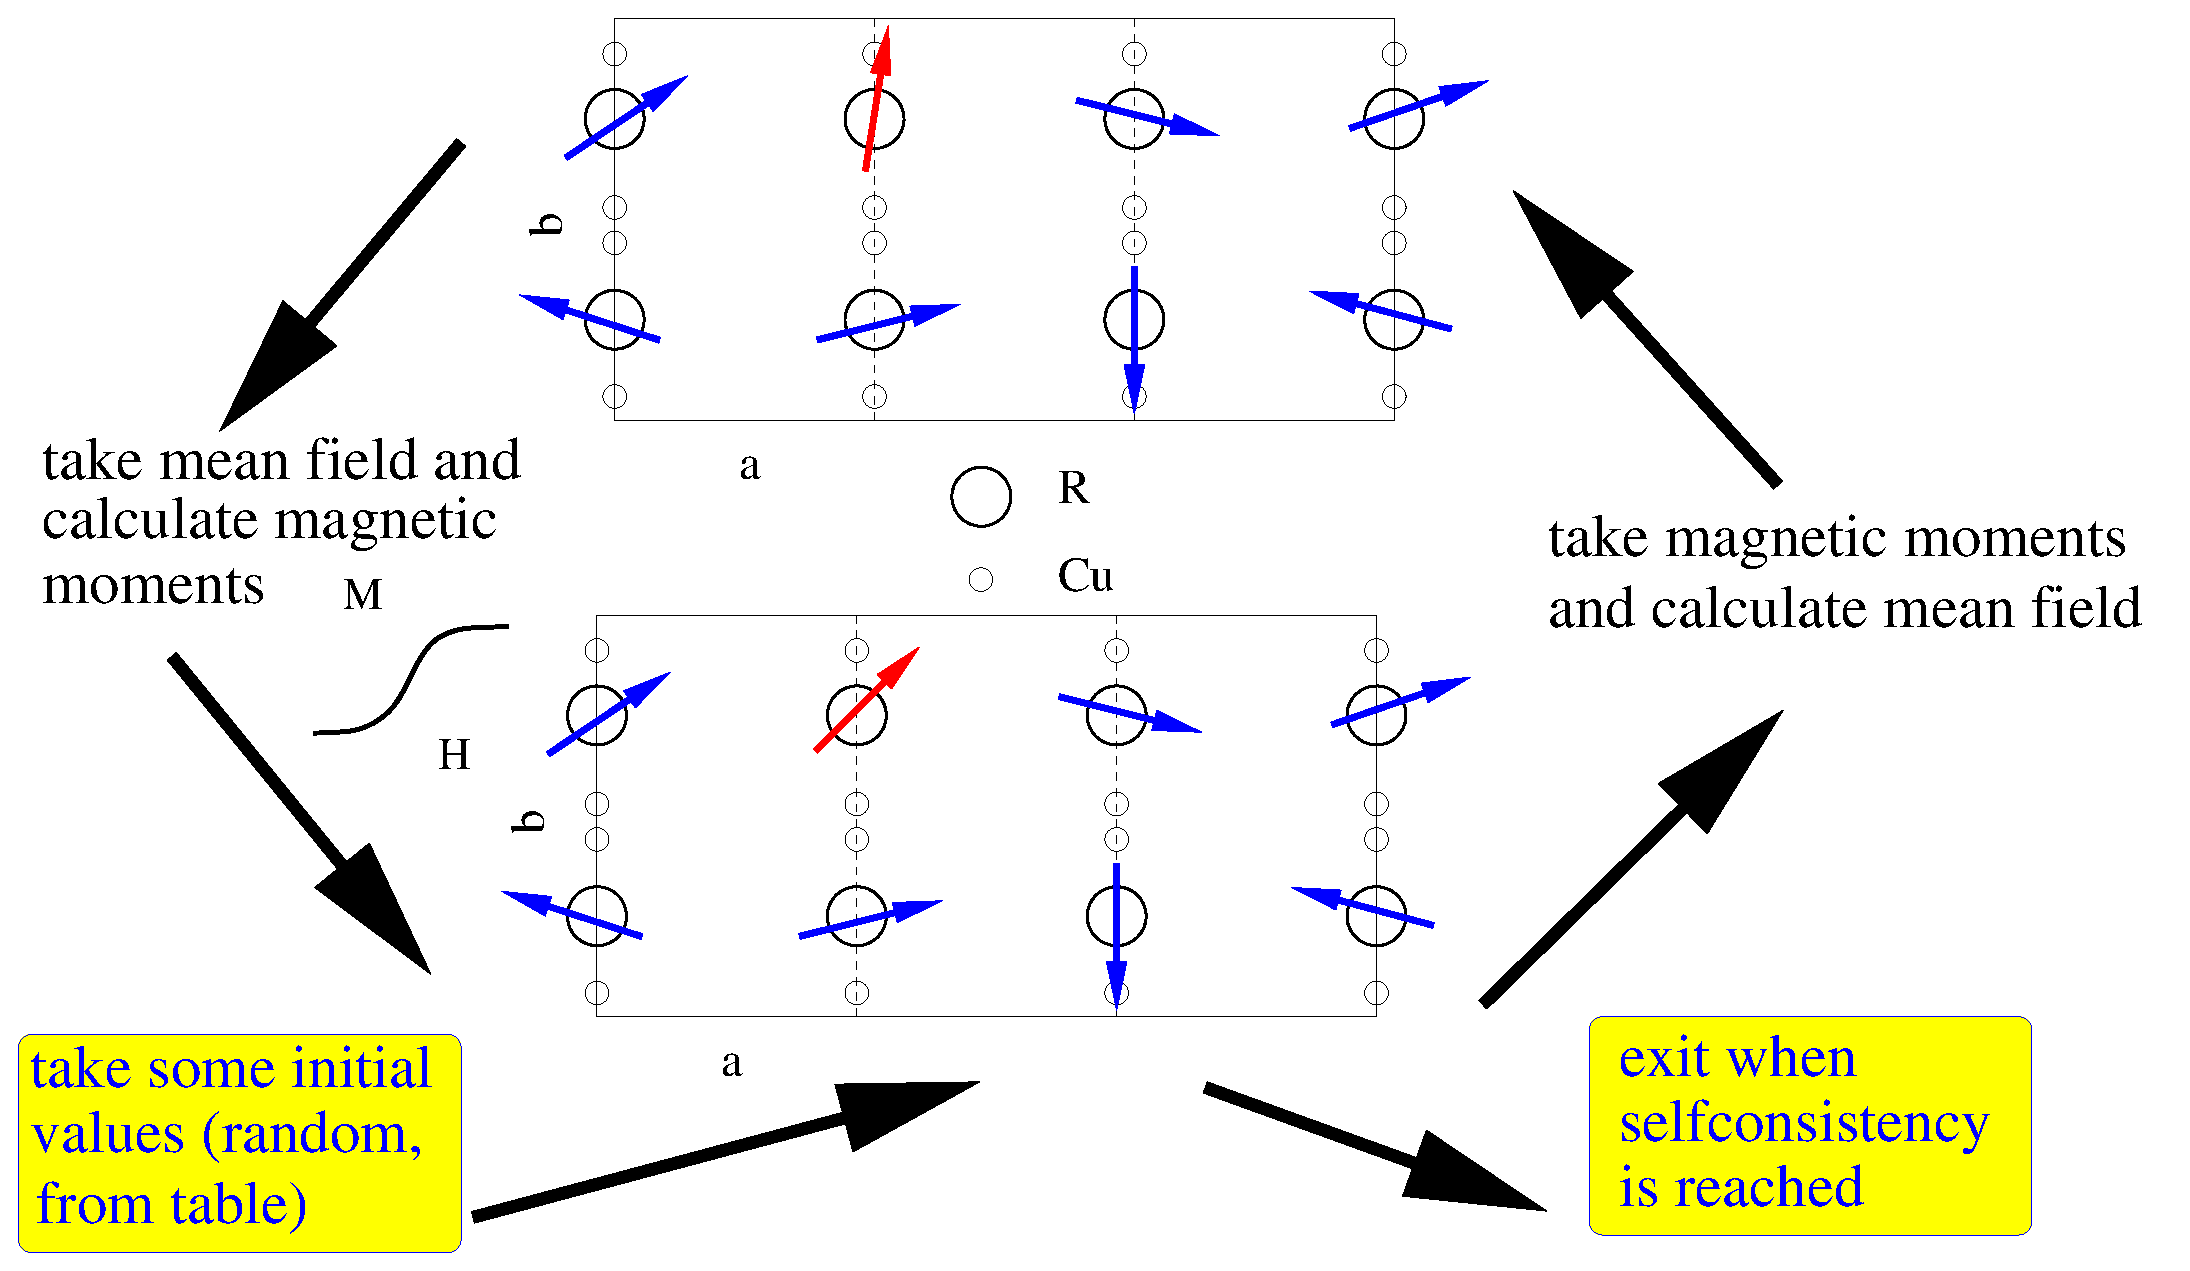
\includegraphics[angle=0,width=0.9\columnwidth]{figsrc/fecalc.eps}
\caption{\label{fecalc}Mean field process of sub {\prg fecalc}.}
\end{figure}

 
\subsubsection{Example {\prg mcphas.ini\index{mcphas.ini}} file for a simple antiferromagnet}

Here is an example of {\prg mcphas.ini\index{mcphas.ini}}, the comments describe the meaning of the different
parameters:

\input{mcphas.ini}



\subsubsection{{\prg mcphas.j\index{mcphas.j}} - lattice and exchange parameters}\label{mcphasj}
This file provides the information about 
the crystallographic
 structure and the magnetic exchange interactions.
For every atom in the crystallographic basis there
has to be given the coordinates, the number of neighbours to be considered, the 
Land\'e factor $g_J$, the single ion property filename and  a set of exchange parameters.
If the exchange parameters (and neighbour positions) are not known for your system, you 
can use the program module {\prg makenn\index{makenn}} (see section \ref{addprog}) to generate 
a list of nearest neighbours and
exchange parameters, currently implemented in {\prg makenn\index{makenn}} are dipolar interactions,
exchange interactions via the Bethe-Slater curve or the RKKY model. Note that in order
to use {\prg makenn\index{makenn}} you have to set up a working {\prg mcphas.j\index{mcphas.j}} file, which may or
may not contain neighbours and interactions.

Use program {\prg addj\index{addj}} to add exchange parameter set stored in different 
such {\prg .j} files (see section~\ref{addprog}).



\begin{description}
\item [Line 1,2:] Comment Lines
\item [Line 3:] lattice constants a,b,c and crystal angles alpha, beta, gamma 
\item [Line 4-6:] primitive lattice vectors
\item [Line 7:] Number of atoms in the primitive crystallographic unit cell ({\prg nofatoms})
\item [Line 8:] a comment line with stars
\item [Line 9:] coordinates  ($d_a$,$d_b$,$d_c$) of 1$^{st}$ magnetic ion in the crystallographic unit cell  with
respect to the lattice vectors $\vec a$,$\vec b$,$\vec c$. The number of neighbours of this 
ion, for which interaction constants are given in the interaction table (nofneighbours). 
If {\prg diagonalexchange}
is set to 0 the 9 components of the exchange tensor are given in column 4-12. 
If {\prg diagonalexchange}
 is 1, only 3 components are given (column 4-6).
If {\prg diagonalexchange}
 is 2, specific components of the exchange tensor can be given in columns 4 onwards. The indices of these components
 must be given in the following line (Line 9a below).
The Land\'e factor of the ion (gJ) and the file name of the corresponding single ion
parameter file (cffilename).
\item [Line 9a:]  If {\prg diagonalexchange=2}, then this line gives the indices of the exchange tensor corresponding to 
 the columns 4 onwards. It must have a variable called {\prg indexexchange} followed by a list of names of components of the interaction
 tensor separated by space. E.g.
 \verb|  #! indexexchange= JaJb JbJc  | 
means column 4 gives the the interaction constant between the
 first angular momentum component of the current ion with the second angular momentum component of its neighbour, whilst 
 column 5 has the interaction constant between the second angular momentum component of this ion with the third component of its
 neighbour. Alternatively, pairs of numbers may be given, as in \verb|  #! indexexchange= 1,2 2,3  |
 Additionally another parameter {\prg symmetricexchange} can be set to 1, where the value in each column is also used 
 for the transposed tensor component. Thus \verb|  #! symmetricexchange=1 indexexchange= JaJb  | is the same as \\
 \verb|  #! indexexchange= JaJb JbJa  | where the 4th and 5th column are the same.
\item [Line 10:]  Comment line
\item [Line 11-(10+nofneighbours):] Interaction table for ion number 1.   
Note: the neighbour coordinates (column 1-3) are given with respect to the lattice vectors
$\vec a$,$\vec b$,$\vec c$. The program then calculates from these values the coordinates
with respect to the primitive lattice $\vec r_1$,~$\vec r_2$,~$\vec r_3$.
($ d_a \vec a + d_b \vec b + d_c \vec c = d_1 \vec r_1 + d_2 \vec r_2 + d_3 \vec r_3$).
Column 4,5,6 \dots contain the components of the interaction tensor $\stackrel{=}{\mathcal J}$. 
Note that in case of non-orthogonal axes the 
components of the moments and the interaction tensor $Ja, Jb, Jc, Jaa, Jbb, Jcc, Jab ...$ 
refer to the orthogonal coordinate system
defined with respect to the nonorthogonal lattice $\vec a,\vec b,\vec c$ as
$Jb||\vec b$, $Jc||(\vec a \times \vec b)$ and $Ja$ perpendicular to $Jb$ and $Jc$.
\item [Line (11+nofneighbours) - end:] for each ion in the unit cell line 8 - (10+nofneighbours)
are repeated.
\end{description}


\vspace{0.5cm}

{\small {\bf Information for experienced users:}
\begin{description}
\item[\prg mcphas.jjj:]
format of exchange parameter file, which only needs a reduced set of exchange
parameters in the input file. Using the program {\prg jjj2j} the file can be transformed
to {\prg mcphas.j\index{mcphas.j}} by adding lines for all the equivalent neighbours. The format definition
of {\prg mcphas.jjj} is the same as {\prg mcphas.j\index{mcphas.j}}, however each line denotes several
equivalent neighbour atoms (instead of only one in {\prg mcphas.j\index{mcphas.j}}) according to the
 following rules:
\begin{itemize}
\item If a nonzero coordinate $d_a$ (or $d_b$,$d_c$) in the interaction table
 corresponds to it's value at the nearest
 lattice point of the primitive lattice,
  additional interactions of the same size
with  neighbours with coordinate $-d_a$ (or $-d_b$,$-d_c$, respectively)
are taken into account. This
holds for each of the three coordinates $d_a$,$d_b$ and $d_c$
 resulting in a maximum
number of 8 equivalent neighbours per line in the interaction table.
\item If the value of $d_a$ (or $d_b$,$d_c$) is zero or differs
from it's value at the nearest lattice point of the primitive lattice, it is 
changed to the value at the nearest lattice point and {\bf no} interaction 
with  neighbours with coordinates $-d_a$ (or $-d_b$,$-d_c$) is
 taken into account. If such
 interaction is needed it may be given in a different line and may
have different magnitude. In this way also crystallographic lattices
with no mirror symmetry may be described.
\end{itemize}
\item[\prg mcphas.coq:]   exchange parameters etc [ in old format]...see examples for details, use {\prg coq2jjj} to 
transform {\prg mcphas.coq} to {\prg mcphas.jjj} format
\end{description}

}


\subsubsection{Example {\prg mcphas.j\index{mcphas.j}} file for a simple antiferromagnet}

Here are example files of a tetragonal antiferromagnet with nearest neighbour interactions, all
files are equivalent:

{\small
\begin{verbatim} 
# simple antiferromagnet 
#<!--mcphase.mcphas.j-->
#***************************************************************
# Lattice Constants (A)
#! a=4.3843 b=4.3843 c=2.4194 alpha=  90 beta=  90 gamma=  90
#! r1a=   1 r2a=   0 r3a=   0
#! r1b=   0 r2b=   1 r3b=   0   primitive lattice vectors [a][b][c]
#! r1c=   0 r2c=   0 r3c=   1
#! nofatoms=1  nofcomponents=3  number of atoms in primitive unit cell/number of components of each spin
# ****************************************************************************
#! da=  0 [a] db=  0 [b] dc=  0 nofneighbours=2 diagonalexchange=0 gJ=0.857143 cffilename=Ce3p.sipf
# da[a] db[b] dc[c] Jaa[meV] Jbb[meV] Jcc[meV] Jab[meV] Jba[meV] Jac[meV] Jca[meV] Jbc[meV] Jcb[meV]
+0	+0	+1	-0.1	-0.1	-0.1   0  0  0  0  0  0
+0	+0	-1	-0.1	-0.1	-0.1   0  0  0  0  0  0
#\end{verbatim}
}

Using diagonalexchange this may be shortened to

{\small
\begin{verbatim} 
# simple antiferromagnet 
#<!--mcphase.mcphas.j-->
#***************************************************************
# Lattice Constants (A)
#! a=4.3843 b=4.3843 c=2.4194 alpha=  90 beta=  90 gamma=  90
#! r1a=   1 r2a=   0 r3a=   0
#! r1b=   0 r2b=   1 r3b=   0   primitive lattice vectors [a][b][c]
#! r1c=   0 r2c=   0 r3c=   1
#! nofatoms=1  nofcomponents=3  number of atoms in primitive unit cell/number of components of each spin
# ****************************************************************************
#! da=  0 [a] db=  0 [b] dc=  0 nofneighbours=2 diagonalexchange=1 gJ=0.857143 cffilename=Ce3p.sipf
# da[a] db[b] dc[c] Jaa[meV] Jbb[meV] Jcc[meV] Jab[meV] Jba[meV] Jac[meV] Jca[meV] Jbc[meV] Jcb[meV]
+0	+0	+1	-0.1	-0.1	-0.1   
+0	+0	-1	-0.1	-0.1	-0.1   
#\end{verbatim}
}

with indexexchange option the sequence of two ion interaction parameters can be changed and
zero parameters may be omitted:

{\small
\begin{verbatim} 
# simple antiferromagnet 
#<!--mcphase.mcphas.j-->
#***************************************************************
# Lattice Constants (A)
#! a=4.3843 b=4.3843 c=2.4194 alpha=  90 beta=  90 gamma=  90
#! r1a=   1 r2a=   0 r3a=   0
#! r1b=   0 r2b=   1 r3b=   0   primitive lattice vectors [a][b][c]
#! r1c=   0 r2c=   0 r3c=   1
#! nofatoms=1  nofcomponents=3  number of atoms in primitive unit cell/number of components of each spin
# ****************************************************************************
#! da=  0 [a] db=  0 [b] dc=  0 nofneighbours=2 diagonalexchange=2 gJ=0.857143 cffilename=Ce3p.sipf
# da[a] db[b] dc[c] Jaa[meV] Jbb[meV] Jcc[meV] Jab[meV] Jba[meV] Jac[meV] Jca[meV] Jbc[meV] Jcb[meV]
#! indexexchange = JaJa JaJc JcJa JbJb JcJc
+0	+0	+1	-0.1 0 0 -0.1	-0.1  
+0	+0	-1	-0.1 0 0 -0.1	-0.1  
#\end{verbatim}
}

{\small
\begin{verbatim} 
# simple antiferromagnet 
#<!--mcphase.mcphas.j-->
#***************************************************************
# Lattice Constants (A)
#! a=4.3843 b=4.3843 c=2.4194 alpha=  90 beta=  90 gamma=  90
#! r1a=   1 r2a=   0 r3a=   0
#! r1b=   0 r2b=   1 r3b=   0   primitive lattice vectors [a][b][c]
#! r1c=   0 r2c=   0 r3c=   1
#! nofatoms=1  nofcomponents=3  number of atoms in primitive unit cell/number of components of each spin
# ****************************************************************************
#! da=  0 [a] db=  0 [b] dc=  0 nofneighbours=2 diagonalexchange=2 gJ=0.857143 cffilename=Ce3p.sipf
# da[a] db[b] dc[c] Jaa[meV] Jbb[meV] Jcc[meV] Jab[meV] Jba[meV] Jac[meV] Jca[meV] Jbc[meV] Jcb[meV]
#! indexexchange = 1,1 1,3, 3,1 2,2 3,3
+0	+0	+1	-0.1 0 0 -0.1	-0.1  
+0	+0	-1	-0.1 0 0 -0.1	-0.1  
#\end{verbatim}
}


using symmetricexchange together with indexexchange will assume that the interaction tensor is symmetic and 
only half of it may be given:

{\small
\begin{verbatim} 
# simple antiferromagnet 
#<!--mcphase.mcphas.j-->
#***************************************************************
# Lattice Constants (A)
#! a=4.3843 b=4.3843 c=2.4194 alpha=  90 beta=  90 gamma=  90
#! r1a=   1 r2a=   0 r3a=   0
#! r1b=   0 r2b=   1 r3b=   0   primitive lattice vectors [a][b][c]
#! r1c=   0 r2c=   0 r3c=   1
#! nofatoms=1  nofcomponents=3  number of atoms in primitive unit cell/number of components of each spin
# ****************************************************************************
#! da=  0 [a] db=  0 [b] dc=  0 nofneighbours=2 diagonalexchange=2 gJ=0.857143 cffilename=Ce3p.sipf
# da[a] db[b] dc[c] Jaa[meV] Jbb[meV] Jcc[meV] Jab[meV] Jba[meV] Jac[meV] Jca[meV] Jbc[meV] Jcb[meV]
#! symmetricexchange=1 indexexchange = JaJa JaJc JbJb JcJc
+0	+0	+1	-0.1 0  -0.1	-0.1  
+0	+0	-1	-0.1 0  -0.1	-0.1  
#\end{verbatim}
}


\subsubsection{Single Ion Property Input Files}\label{sifile}

In order to speed up calculations or treat special problems a large 
variety of single ion modules is available. This includes the
option to load a user written single ion module. Details are 
given in chapter~\ref{simod}.

The first time user of {\prg McPhase} should use the module {\prg so1ion}\index{so1ion} and 
create an appropriate single ion property input file as described in
section \ref{cf1ion}. A good starting point are several examples
given in directory {\prg examples}.


\subsubsection{Example single ion property file  for a simple antiferromagnet}

Here is an example file {\prg mcphas.cf1} describing the anisotropy of a 
simple antiferromagnet with Ce atoms having basal plane anisotropy. Note the
axis convention xyz$||$abc, in case of non-orthogonal axes the convention 
is $y||\vec b$, $z||(\vec a \times \vec b)$ and $x$ perpendicular to $y$ and $z$.


\input{mcphas.cf1}

\subsubsection{{\prg mcphas.tst\index{mcphas.tst}} - input file of test spin-configurations (optional)}
This file is optional and contains
some test momentum configurations to be used for the calculation
             of the free energy. Mind that
\begin{itemize}
\item  in the file header the number of atoms in the primitive
       crystallographic unit cell and the number of components
       of the spin vector have to be given.
\item  at the end of the
 file there must be no empty lines !
\end{itemize}

The momentum - configurations tables always refer to spins sitting on
the primitive lattice ${\mbf r}_i$. If more than one atom is in
the primitive basis, the momentum gets $3n$ components ($n=$ number
of atoms in the crystallographic basis). See {\prg ./examples/ndcu2b\_new/} for
examples of a two atom basis. Units of these tables are that of total 
angular momentum $<J>$.

\subsubsection{Example {\prg mcphas.tst\index{mcphas.tst}} file  for a simple antiferromagnet}

Here is the file {\prg mcphas.tst\index{mcphas.tst}} for the simple antiferromagnet example
describing some spin configurations
to be used as starting values for the mean field process:

\input{mcphas.tst}
Note, in case of non-orthogonal axes the convention 
is $mb||\vec b$, $mc||(\vec a \times \vec b)$ and $ma$ perpendicular to $mb$ and $mc$.

\subsubsection{subdirectory {\prg ./results} - directory where calculated data is stored}

In order to be able to save the results of a calculation the directory {\prg ./results} has to
exist. Mind that all files in this directory will be overwritten without warning. 

\subsubsection{subdirectory {\prg ./fit} - experimental data for fit (optional) } 

In order that {\prg McPhase} can calculate the standard deviation between
 experimental data and the results of the simulation, some experimental data
 can be given in the subdirectory {\prg ./fit}. The filenames and the data-format
 are the same as the output files of {\prg McPhas}, e.g. {\prg mcphas.fum}, {\prg mcphas.hkl}
 etc. {\prg McPhase} looks into the directory {\prg ./fit} and if it finds any
 of these files, the standard deviation is increased correspondingly. 

What measurement data can be used to calculate a standard deviation ?

\begin{description}
\item[{\prg mcphas.fum}] if given in column 11, 12, 13 in {\prg ./fit/mcphas.fum} the
            magnetisation in the $a$, $b$ and $c$ direction is used for calculation
	    of the standard deviation sta. The standard deviation is calculated
	    as ${\rm sta}=\sum_{\rm data points i} ({\mbf m}_i^{calc}-{\mbf m}_i^{meas})^2$.
	    All three components of the magnetic moment have to be given and are used.

\end{description}

Note that the measured data has to be given in those (H-T) points which are 
calculated by mcphas\index{mcphas} in order to be used by the program to increase {\prg sta}.
It is usually most effective to fit only few data points, because a large set
of data points will not improve the quality of the fit and only require a large
amount of calculation time.



\subsection{Starting a simulation}
\label{start}

To start the simulation goto the directory containing the
input files {\prg mcphas.ini, mcphas.j, etc. } and type

\begin{description}
\item[\prg mcphas] to run the program generating stepwise $H-T$ values 
              in a loop given by {\prg mcphas.ini\index{mcphas.ini}} (you can also press the
              symbol in the {\prg McPhase - Explorer} window).
\item[\prg mcphas\index{mcphas} [file]]  to run the program with an input file --   
             {\prg file} contains T ha hb hc values to be calculated 
             if [file] is not given, xmin xmax xstep (xT xHa xHb xHc)
             ymin ymax ystep (yT yHa yHb yHc) is read from file {\prg mcphas.ini\index{mcphas.ini}}
	     and phase diagram is calculated
\item[\prg mcphas\index{mcphas} -h]  to  print help and version of {\prg McPhas}.
\item[\prg mcphas\index{mcphas} -stamax 14]  end mcphas\index{mcphas} if standard deviation exceeds 14.
\item[\prg mcphas\index{mcphas} -a] avoid overwriting output files in results, append new results to existing files
\item[\prg mcphas\index{mcphas} -v]  to  enable verbose mode with lots of messages of {\prg McPhas}. Specifically
the verbose mode enables the following features:
  \begin{itemize}
			          \item more information is printed out, 
			          \item the q-vectors file {\prg ./results/mcphas.qvc} will contain 
				    the explicit spin configurations
			          \item the display\index{display} on screen (ghostview window using 
				     {\prg ./results/.sps.eps}) will be updated not only 
				    when a H-T point has been finished but always 
				    when a structure with smaller free energy 
				    has been stabilised
  \end{itemize}
\item[\prg mcphasit\index{mcphas}] to start mcphase in commandline mode without opening any window
\end{description}

\vspace{1cm}
{\em Exercises:}
\begin{itemize}
\item Look at the input files for {\prg McPhase} given in the directory
{\prg examples/ndcu2b\_new}.  How many atoms are contained in the crystallographic basis ?
\item
Start the simulation by typing the command {\prg mcphas}.
\end{itemize}



\subsection{Options for a running simulation}
... when the program is running, the options in the main window
can be changed. Pressing ''displayall'' displays the current spin-configuration
at each iteration step. Pressing ''log fe vs Q'' appends free energy vs Q
data to {\prg mcphas.log} for every ($T-H$) point.


The file {\prg ./results/.spins.eps} is used to show the information about the currently calculated
spin structure on the screen using the postscript file viewer ghostview.

The file {\prg ./results/.mcphas.fum} contains the information of the magnetisation curve
which is currently calculated. This information is automatically displayed on the screen.


The program {\prg display} (see section \ref{display}) can be used 
for the online display\index{display} of any other
curve(s).


\subsection{Output Files - {\prg mcphas.qvc,phs,sps,mf,fum,j1...,xyt,hkl} }\label{outputfiles}
 (in directory ./results/ after a simulation run) 

\begin{figure}[htb]%h=here, t=top, b=bottom, p=separate figure page
\begin{center}\leavevmode
\includegraphics[angle=0, width=0.3\textwidth]{figsrc/magnetization_ndcu2.ps}
\end{center}
\caption{Calculated magnetisation of NdCu$_2$ for field parallel to the orthorhombic $b$-direction.}
\label{magnetization}
\end{figure}

\begin{figure}[htb]%h=here, t=top, b=bottom, p=separate figure page
\begin{center}\leavevmode
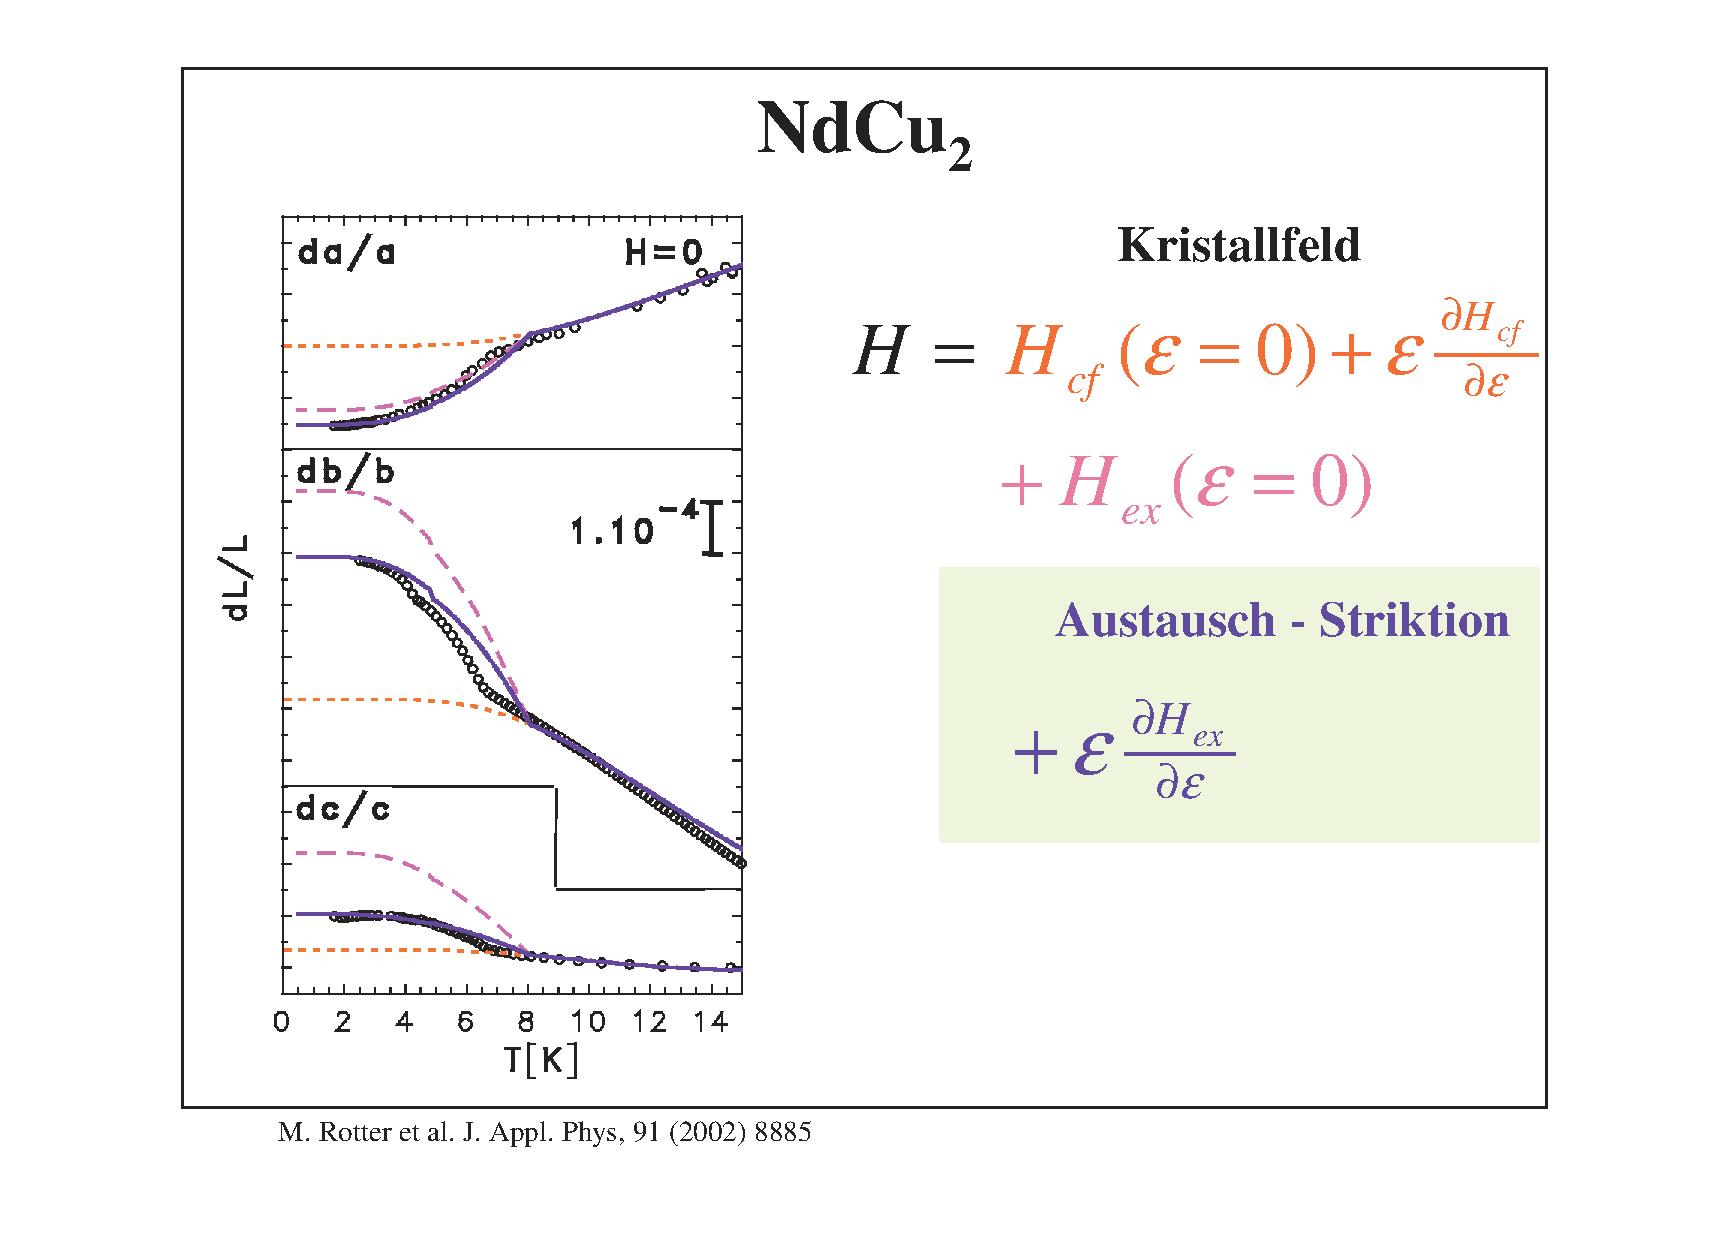
\includegraphics[angle=0, width=0.8\textwidth]{figsrc/magnetostriction_ndcu2.eps}
\end{center}
\caption{Calculated spontaneous magnetostriction of NdCu$_2$.}
\label{magnetostrictiongraphic}
\end{figure}

\begin{description}
\item [\prg mcphas.qvc]    the set of test q-vectors used for calculation of free energy.
                           Components of these q vectors refer to the reciprocal lattice $\vec a^*,\vec b^*,\vec c^*$.
\item [\prg mcphas.phs]    spin-configuration table of different types of spin-configurations. 
                            Note, in case of non-orthogonal axes the convention in these tables 
                            is $mb||\vec b$, $mc||(\vec a \times \vec b)$ and $ma$ perpendicular to $mb$ and $mc$.

                           {\em Note}: 
                           there is no natural criteria for deciding, if one spin-configuration is
			   different from another one. Therefore the list of ''different''
			   spin-configurations is dependent on the meaning of ''different''.
			   
			   The program {\prg McPhase} decides whether a spin-configuration is
			   different from another by a simple criteria, namely by the
			   angle between the spins. Comparing two spin configurations it calculates
			   the angle between corresponding spins and if for one spin the
			   angle is not small, the configuration is treated as a different
			   configuration. Therefore for example a ferromagnet with moments
			   in $a$ has a different spin configuration than a ferromagnet with
			   moments in $b$ direction. 
\item [\prg mcphas.sps]    $T-H$ dependence of spin-configuration. The spin configurations stored in this
                           file may be displayed using the program {\prg spins\index{spins}}, an example is given
			   in figure~\ref{spingraphic}.
                            Note, in case of non-orthogonal axes the convention for applied field $Ha, Hb,Hc$ and
                            also for the moment components $ma, mb, mc$ in these tables 
                            is $mb||\vec b$, $mc||(\vec a \times \vec b)$ and $ma$ perpendicular to $mb$ and $mc$.

\item [\prg mcphas.mf]     $T-H$ dependence of exchange field configuration, stored as $g_J \mu_B H_{xc}(i)$(unit is in meV)
                            for i=1,2,...,number of spins in magnetic unit cell.
                            Note, in case of non-orthogonal axes the convention for applied field $Ha, Hb,Hc$ and
                            also for the mean field components in these tables 
                            is $Hb||\vec b$, $Hc||(\vec a \times \vec b)$ and $Ha$ perpendicular to $Hb$ and $Hc$.
\item [\prg mcphas.fum]    free energy, magnetic energy (the derivative with respect to temperature gives the specific %%@
heat),
                           magnetisation data and (if cfield is used with higher order interactions)
                           expectation values of the Stevens Operators $<O_l^m>$ . As an example for the information
			   contained in this file the calculated magnetisation and magnetostriction of NdCu$_2$ is shown in
			   figures~\ref{magnetization} and ~\ref{magnetizationgraphic}.
                            Note, in case of non-orthogonal axes the convention for applied field $Ha, Hb,Hc$ and
                            also for the magnetisation components $ma,mb,mc$ in these tables 
                            is $Hb||\vec b$, $Hc||(\vec a \times \vec b)$ and $Ha$ perpendicular to $Hb$ and $Hc$.

\item [\prg mcphas1.j1 .j1 .j2 ...] 
               spin-spin correlation functions for sub-lattice 1 neighbour 1 2 ...
	       (linear combination is proportional to magnetostriction)
	       The spin-spin correlation functions for neighbour $k$ are defined by
	       the following sum of dyadic products:

	       \begin{equation}
	        \frac{1}{n}\sum_{s=1}^n <{\mbf J}^s> \times  <{\mbf J}^{s+k}>
	       \end{equation}
	       with $n$ being the number of moments in the magnetic unit cell.
	       Single ion and two-ion magnetostriction can be calculated using the $<O_l^m>$ and the
	       spin-spin correlation functions. As an example the magnetostriction analysis of
	       NdCu$_2$ is shown in figure~\ref{magnetostrictiongraphic}. For details 
             please refer to~\cite{rotter02-8885}.
                            Note, in case of non-orthogonal axes the convention for applied field $Ha, Hb,Hc$ and
                            also for the moment components in these tables 
                            is $Hb||\vec b$, $Hc||(\vec a \times \vec b)$ and $Ha$ perpendicular to $Hb$ and $Hc$.
\item [\prg mcphas.xyt]    phase diagram as x,y,T, H, phase-number j according to spin-configuration table
               given in mcphas.phs, a periodicity key, nettomoments <J>.
 Figure~\ref{phasediagramgraphic}
	       shows the phase diagram of NdCu$_2$ for magnetic fields parallel to the orthorhombic $b$-direction.
                            Note, in case of non-orthogonal axes the convention for applied field $Ha, Hb,Hc$ 
                             in these tables 
                            is $Hb||\vec b$, $Hc||(\vec a \times \vec b)$ and $Ha$ perpendicular to $Hb$ and $Hc$.
\item [\prg mcphas.hkl]    calculated (unpolarised) neutron diffraction data (the calculated magnetic intensities
    correspond to the magnetic structure + Polarisation factor. The
    Lorentz-factor , magnetic form factor and  instrumental corrections are not calculated.)
 As an example figure~\ref{neutintgraphic}
    shows the calculated temperature dependence of magnetic amplitudes for NdCu$_2$.
                           $h,k,l$ refer to the reciprocal lattice $\vec a^*,\vec b^*,\vec c^*$.
                            Note, in case of non-orthogonal axes the convention for applied field $Ha, Hb,Hc$ 
                             in these tables 
                            is $Hb||\vec b$, $Hc||(\vec a \times \vec b)$ and $Ha$ perpendicular to $Hb$ and $Hc$.
    
\item [\prg mcphasa.hkl]    Fourier Transform of the $a$-component of the magnetic Moments.
                           $h,k,l$ refer to the reciprocal lattice $\vec a^*,\vec b^*,\vec c^*$.
                            Note, in case of non-orthogonal axes the convention for applied field $Ha, Hb,Hc$ and
                            the magnetic moment component in these tables 
                            is $Hb||\vec b$, $Hc||(\vec a \times \vec b)$ and $Ha$ perpendicular to $Hb$ and $Hc$.
\item [\prg mcphasb.hkl]    Fourier Transform of the $b$-component of the magnetic Moments.
                           $h,k,l$ refer to the reciprocal lattice $\vec a^*,\vec b^*,\vec c^*$.
                            Note, in case of non-orthogonal axes the convention for applied field $Ha, Hb,Hc$ and
                            the magnetic moment component in these tables 
                            is $Hb||\vec b$, $Hc||(\vec a \times \vec b)$ and $Ha$ perpendicular to $Hb$ and $Hc$.
\item [\prg mcphasc.hkl]    Fourier Transform of the $c$-component of the magnetic Moments.
                           $h,k,l$ refer to the reciprocal lattice $\vec a^*,\vec b^*,\vec c^*$.
                            Note, in case of non-orthogonal axes the convention for applied field $Ha, Hb,Hc$ and
                            the magnetic moment component in these tables 
                            is $Hb||\vec b$, $Hc||(\vec a \times \vec b)$ and $Ha$ perpendicular to $Hb$ and $Hc$.
\end{description} 

\vspace{1cm}
{\em Exercises:}
\begin{itemize}
\item Look at the output files of {\prg McPhase}  in the directory
{\prg examples/ndcu2b\_new/results}.  At which magnetic field
the ferromagnetically aligned state is achieved (at $T=$2~K)?
\item
What is the propagation vector in the different antiferromagnetic phases at $T=$2~K ?
\end{itemize}



\subsubsection{{\prg mcphas.tst\index{mcphas.tst}} - input file of test spin-configurations (optional)}
This file is optional and contains
some test momentum configurations to be used for the calculation
             of the free energy. Mind that
\begin{itemize}
\item  in the file header the number of atoms in the primitive
       crystallographic unit cell and the number of components
       of the spin vector have to be given.
\item  at the end of the
 file there must be no empty lines !
\end{itemize}

The momentum - configurations tables always refer to spins sitting on
the primitive lattice ${\mbf r}_i$. If more than one atom is in
the primitive basis, the momentum gets $3n$ components ($n=$ number
of atoms in the crystallographic basis). See {\prg ./examples/ndcu2b\_new/} for
examples of a two atom basis. Units of these tables are that of total 
angular momentum $<J>$.

\subsubsection{Example {\prg mcphas.tst\index{mcphas.tst}} file  for a simple antiferromagnet}

Here is the file {\prg mcphas.tst\index{mcphas.tst}} for the simple antiferromagnet example
describing some spin configurations
to be used as starting values for the mean field process:

\section{{\prg mcphas} - calculation of thermodynamic properties (Magnetisation, Susceptibility, Specific Heat, Neutron %%@
Diffraction, etc.)}
\label{runmcphas}

In order to perform calculations beyond the capabilities of {\prg cfield\index{cfield}} it is necessary
to use the program {\prg mcphas}. 
\begin{itemize}
\item As a first step it is possible to
calculate the thermodynamic properties such as magnetisation or specific heat
considering only single ion effects. In this case all the exchange parameters
have to be set to zero in {\prg mcphas.j\index{mcphas.j}}. 
\item for more advanced calculations the two - ion interactions have to be
considered and may lead to magnetic order. {\prg mcphas} can perform 
calculations in the ordered state in the following way: for 
a given temperature $T$ and magnetic field $\mbf H$ (vector)
several possible magnetic structures are stabilised
by a mean field algorithm and the free energy is 
calculated. The initial values for this mean-field procedure are
modified by a Monte Carlo process.


The temperature and magnetic field is varied during the calculation
and thereby it is possible to map out the magnetic phase diagram.
\end{itemize}

The program produces a plot of the stabilised magnetic
structures and the magnetisation on screen, the
output files contain additional information 
such as calculated magnetoelastic and  neutron-scattering
data. Several graphic programs easy the visualisation of the
calculated data (section~\ref{graphics}).



\subsection{Input Files}
The program {\prg McPhase} needs the following input files (all in the same directory)
 in order to run:

\begin{enumerate}
\item {\prg mcphas.ini\index{mcphas.ini}}
 - controlling the algorithm
\item {\prg mcphas.j\index{mcphas.j}}
  - lattice and exchange parameters
\item {\prg mcphas.tst\index{mcphas.tst}(optional)}  - test spin configurations
\item {\prg single-ion property files}
\item {\prg directory ./results/}
 - directory where calculated data is stored
\item {\prg directory ./fit} - experimental data for fit (optional)
\end{enumerate}


 All
 of these input files have to be in one directory and the program
has to be started in this directory. The results of the simulation
are then stored in the  subdirectory ./results/, which must exist before starting
the program 
... see directory ./examples/ for some examples.
 In order to prepare these files
for a new calculation it is best to take them from an example, copy the files
to a new directory and make the
modifications  to adapt them to the new problem.

\subsubsection{Example - a simple antiferromagnet}

In the following description of the input files we will always refer
to a simple example: a simple antiferromagnet
on a primitive orthorhombic lattice. The first time user
will thus have a simple example to follow, all corresponding
files are given in the directory {\prg tutorial/03magnetic\_phases\_mcphas/simpleAF}.
 

\subsubsection{{\prg mcphas.ini\index{mcphas.ini}} - controlling the algorithm}
   Initial file containing algorithm control parameters, for instance the range and spacing of
   propagation vectors Q or the number of Monte Carlo trials for initial spin configurations
    - {\em mind}: this
   file is rewritten and reread  when running the program and may be changed by the
   user in order to manipulate the running simulation.

{\prg mcphas.ini\index{mcphas.ini}} consists of several sections:
\begin{description}
\item [MCPHASE RUNTIME CONTROL:] this section contains the parameters
controlling the status of the calculation.
\item [XY PHASEDIAGRAM PARAMETERS:] here the temperature and field range and
step widths of the calculation are specified.
The definition of the x and y
axis in terms of temperature and magnetic field is followed by the
corresponding range and step width. An offset may be given for all
field and temperature values.
Note that for most cases of interest
this offset is zero (T0=0, Ha0=0, Hb0=0, Hc0=0).
 For the simple case of calculating a Temperature-Field phase diagram
 It is just necessary to set xT=1 and give the temperature range by
xmin/xmax/xstep. For field in b direction then just set yHb=1 and 
define the range in ymin/ymax/ystep.
In case of non-orthogonal axes the applied magnetic field
components $Ha, Hb, Hc$ refer to the orthogonal coordinate system
defined with respect to the nonorthogonal lattice $\mbf a,\mbf b,\mbf c$ as
$Hb||\mbf b$, $Hc||(\mbf a \times \mbf b)$ and $Ha$ perpendicular to $Hb$ and $Hc$.

\item [GENERATION OF SPINCONFIGURATIONS:] at the beginning of the program
some initial values of spin configurations are generated from a set of 
propagation vectors. This section defines the range of propagation vectors
and the step width.
Depending on the value of the propagation Q with respect to the primitive reciprocal lattice
1-, 2- or 3-dimensional simulations of magnetic lattices
are possible. It is advisable to 
think carefully about the chosen range and spacing of Q vectors in order
to limit calculation time.
 
For example a good starting point is to begin with a calculation with large
step widths (e.g. 0.1)  covering the Brillouin zone. This should give an idea
of the propagation vectors which are stabilised. An advanced calculation
could then fine tune the propagation and determine its accurate value (using
small step widths in a limited area of the zone).
The verbose option of {\prg mcphas} allows to inspect the propagation vectors
which are actually used in the calculation.
Trick: in order to get a quick overview of the
q-vector range covered by the mcphas\index{mcphas} simulation start mcphas, exit and 
just type {\prg felog ./results/mcphas.qvc} (need {\prg perl,perldl,pdl,pgplot} packages).

In order to limit calculation time, the maximum periodicity
of the magnetic unit cell with respect to the crystallographic unit cell 
(maxqperiod) and the maximum number of spins in the magnetic unit cell 
(maxnofspins) can be limited. Also the maximum number of test spin configurations
in the internal table can be limited (maxnoftestspincf).
A critical feature with respect to calculation time is also the number of
spin configurations which are generated by a random process from a tabulated
SPINCONFIGURATIONS during the calculation. 

In summary the variables in this section are mainly important to adapt the
program to a given computer system with finite speed. They have to be set
to optimise between speed and accuracy of the calculation. In order to
find appropriate values it is best to perform some calculations 
and restrict the parameters step by step if insufficient speed is obtained.
Also the examples included in the program package may serve as starting
points.

\item [PARAMETERS FOR SUB FECALC SELFCONSISTENCY PROCESS:] the most important
procedure in the module {\prg mcphas} is the sub fecalc. In this part of the 
program the self consistent calculation of the magnetic moment configuration
is performed as shown schematically in fig.~\ref{fecalc}. 
In the mean field approximation the Hamiltonian~(\ref{hamilton}) is approximated
by

\begin{equation}
 {\mathcal H}=\sum_n H_{SI}^n + E_{corr}
\end{equation}

with the single ion Hamiltonian (in case of module {\prg so1ion\index{so1ion}})

\begin{equation}
H_{SI}^n=  B_l^m O_{lm}({\mbf J}^n) 
	     - g_{Jn} \mu_B {\mbf J}^n {\mbf H^n_{eff}} 
\end{equation}

and the correction term

\begin{equation}
E_{corr}=\frac{1}{2}\sum_{n} g_{Jn} \mu_B \langle {\mbf J}^n
 \rangle (\mbf H^n_{eff}-\mbf H) 
\end{equation}

and with the mean fields $ \mbf H^n_{eff}$ given by

\begin{equation}\label{meanfield}
\mbf H^n_{eff}=\mbf H + \mbf H^n_{xc}=\mbf H+\sum_{{\mbf G'}n'} \frac{{\mathcal J}
(\mbf r_n-(\mbf G'+\mbf r_{n'}))}{g_{Jn}\mu_B } \langle{\mbf
J}^{n'}\rangle
\end{equation}

These mean fields and the moments $\langle \mbf J^n \rangle$ 
are determined in a self consistent
way. For a given magnetic unit cell and initial configuration 
of magnetic moments
the mean fields are calculated according to equation~(\ref{meanfield}). 
Then, for each
magnetic ion the single ion property module is taken 
and the magnetic moment $\langle \mbf J^n \rangle$ is 
calculated from it's mean field. The mean fields are used again in equation~(\ref{meanfield})
and so on .... until convergence is reached. 
Then, the free energy ($f=-kT\sum_n \ln(z_n) + E_{corr}$ ) 
of the stabilised
configuration is calculated (this is why this sub is called {\prg fecalc}). 
The free energies of a lot of different stabilised configurations have to
be compared in order to find out which configuration has lowest free energy, i.e.
is stable in thermal  equilibrium.

It may happen that this process does
not converge due to bad choice of the initial configuration, therefore a maximum number
of mean field loops has to be given by the user.
The results of a calculation may be significantly influenced by
changing parameters such as the maximum number of iteration loops 
in this section. 
In fact the simulation is always a compromise of calculation time and accuracy: if only
a few initial spin configurations are tried at each (H-T) point, the calculation speed is
fast, however it is possible that the program misses the magnetic structure with the
lowest free energy. The same holds if other critical parameters of the simulation are
restricted too much.
 

\item [OUTPUT OF PHYSICAL PROPERTIES:]
Some options for the output of the calculation can be changed in this section.
\end{description}

\begin{figure}[hb]
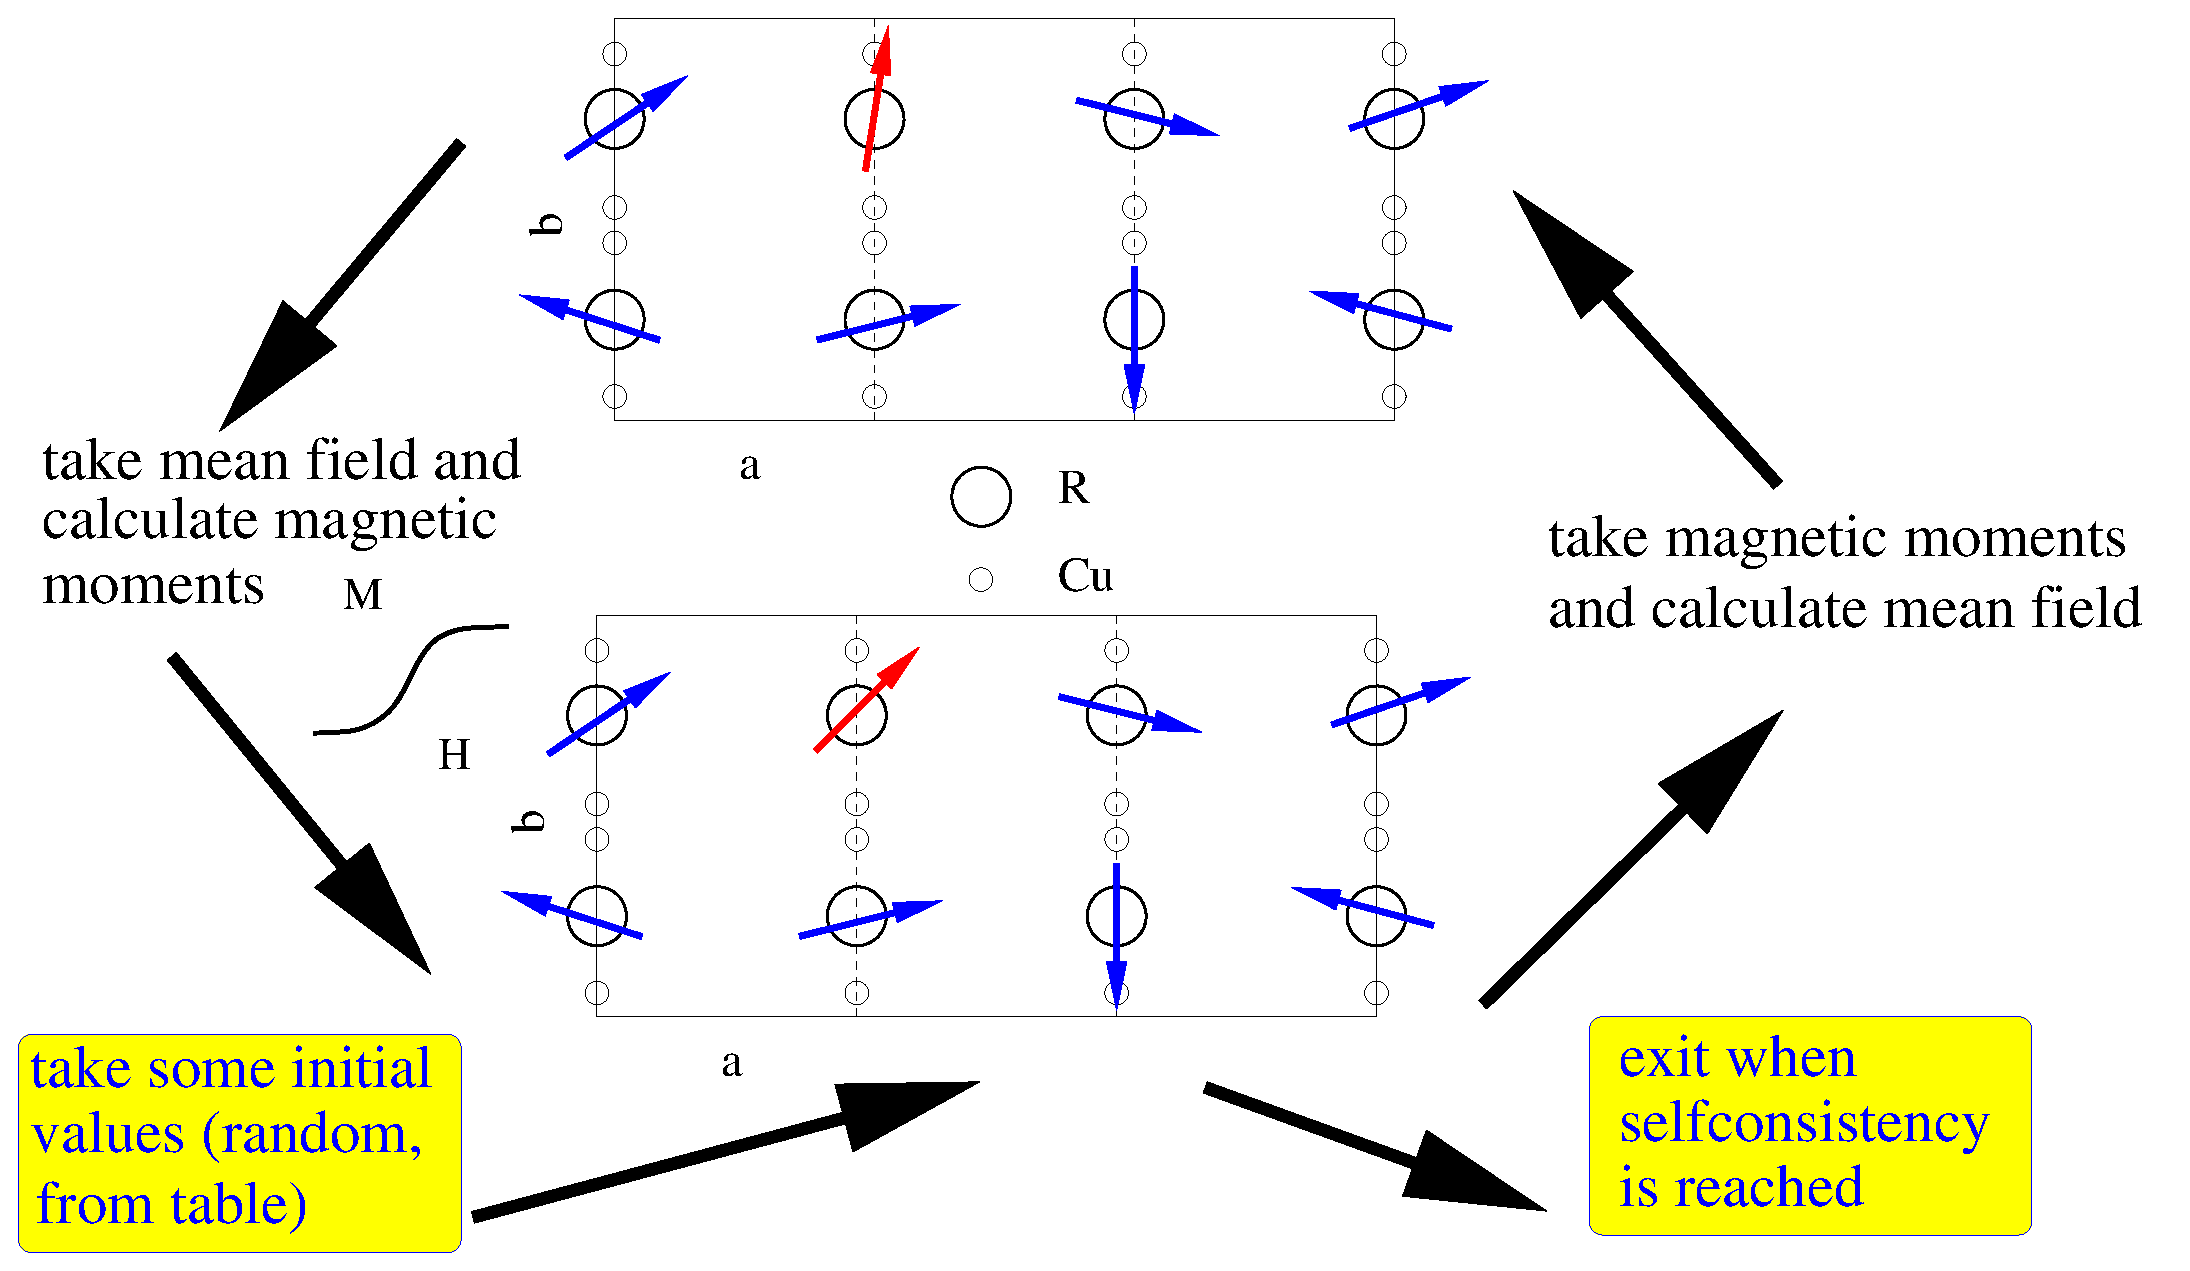
\includegraphics[angle=0,width=0.9\columnwidth]{figsrc/fecalc.eps}
\caption{\label{fecalc}Mean field process of sub {\prg fecalc}.}
\end{figure}

 
\subsubsection{Example {\prg mcphas.ini\index{mcphas.ini}} file for a simple antiferromagnet}

Here is an example of {\prg mcphas.ini\index{mcphas.ini}}, the comments describe the meaning of the different
parameters:

\input{mcphas.ini}



\subsubsection{{\prg mcphas.j\index{mcphas.j}} - lattice and exchange parameters}\label{mcphasj}
This file provides the information about 
the crystallographic
 structure and the magnetic exchange interactions.
For every atom in the crystallographic basis there
has to be given the coordinates, the number of neighbours to be considered, the 
Land\'e factor $g_J$, the single ion property filename and  a set of exchange parameters.
If the exchange parameters (and neighbour positions) are not known for your system, you 
can use the program module {\prg makenn\index{makenn}} (see section \ref{addprog}) to generate 
a list of nearest neighbours and
exchange parameters, currently implemented in {\prg makenn\index{makenn}} are dipolar interactions,
exchange interactions via the Bethe-Slater curve or the RKKY model. Note that in order
to use {\prg makenn\index{makenn}} you have to set up a working {\prg mcphas.j\index{mcphas.j}} file, which may or
may not contain neighbours and interactions.

Use program {\prg addj\index{addj}} to add exchange parameter set stored in different 
such {\prg .j} files (see section~\ref{addprog}).



\begin{description}
\item [Line 1,2:] Comment Lines
\item [Line 3:] lattice constants a,b,c and crystal angles alpha, beta, gamma 
\item [Line 4-6:] primitive lattice vectors
\item [Line 7:] Number of atoms in the primitive crystallographic unit cell ({\prg nofatoms})
\item [Line 8:] a comment line with stars
\item [Line 9:] coordinates  ($d_a$,$d_b$,$d_c$) of 1$^{st}$ magnetic ion in the crystallographic unit cell  with
respect to the lattice vectors $\vec a$,$\vec b$,$\vec c$. The number of neighbours of this 
ion, for which interaction constants are given in the interaction table (nofneighbours). 
If {\prg diagonalexchange}
is set to 0 the 9 components of the exchange tensor are given in column 4-12. 
If {\prg diagonalexchange}
 is 1, only 3 components are given (column 4-6).
If {\prg diagonalexchange}
 is 2, specific components of the exchange tensor can be given in columns 4 onwards. The indices of these components
 must be given in the following line (Line 9a below).
The Land\'e factor of the ion (gJ) and the file name of the corresponding single ion
parameter file (cffilename).
\item [Line 9a:]  If {\prg diagonalexchange=2}, then this line gives the indices of the exchange tensor corresponding to 
 the columns 4 onwards. It must have a variable called {\prg indexexchange} followed by a list of names of components of the interaction
 tensor separated by space. E.g.
 \verb|  #! indexexchange= JaJb JbJc  | 
means column 4 gives the the interaction constant between the
 first angular momentum component of the current ion with the second angular momentum component of its neighbour, whilst 
 column 5 has the interaction constant between the second angular momentum component of this ion with the third component of its
 neighbour. Alternatively, pairs of numbers may be given, as in \verb|  #! indexexchange= 1,2 2,3  |
 Additionally another parameter {\prg symmetricexchange} can be set to 1, where the value in each column is also used 
 for the transposed tensor component. Thus \verb|  #! symmetricexchange=1 indexexchange= JaJb  | is the same as \\
 \verb|  #! indexexchange= JaJb JbJa  | where the 4th and 5th column are the same.
\item [Line 10:]  Comment line
\item [Line 11-(10+nofneighbours):] Interaction table for ion number 1.   
Note: the neighbour coordinates (column 1-3) are given with respect to the lattice vectors
$\vec a$,$\vec b$,$\vec c$. The program then calculates from these values the coordinates
with respect to the primitive lattice $\vec r_1$,~$\vec r_2$,~$\vec r_3$.
($ d_a \vec a + d_b \vec b + d_c \vec c = d_1 \vec r_1 + d_2 \vec r_2 + d_3 \vec r_3$).
Column 4,5,6 \dots contain the components of the interaction tensor $\stackrel{=}{\mathcal J}$. 
Note that in case of non-orthogonal axes the 
components of the moments and the interaction tensor $Ja, Jb, Jc, Jaa, Jbb, Jcc, Jab ...$ 
refer to the orthogonal coordinate system
defined with respect to the nonorthogonal lattice $\vec a,\vec b,\vec c$ as
$Jb||\vec b$, $Jc||(\vec a \times \vec b)$ and $Ja$ perpendicular to $Jb$ and $Jc$.
\item [Line (11+nofneighbours) - end:] for each ion in the unit cell line 8 - (10+nofneighbours)
are repeated.
\end{description}


\vspace{0.5cm}

{\small {\bf Information for experienced users:}
\begin{description}
\item[\prg mcphas.jjj:]
format of exchange parameter file, which only needs a reduced set of exchange
parameters in the input file. Using the program {\prg jjj2j} the file can be transformed
to {\prg mcphas.j\index{mcphas.j}} by adding lines for all the equivalent neighbours. The format definition
of {\prg mcphas.jjj} is the same as {\prg mcphas.j\index{mcphas.j}}, however each line denotes several
equivalent neighbour atoms (instead of only one in {\prg mcphas.j\index{mcphas.j}}) according to the
 following rules:
\begin{itemize}
\item If a nonzero coordinate $d_a$ (or $d_b$,$d_c$) in the interaction table
 corresponds to it's value at the nearest
 lattice point of the primitive lattice,
  additional interactions of the same size
with  neighbours with coordinate $-d_a$ (or $-d_b$,$-d_c$, respectively)
are taken into account. This
holds for each of the three coordinates $d_a$,$d_b$ and $d_c$
 resulting in a maximum
number of 8 equivalent neighbours per line in the interaction table.
\item If the value of $d_a$ (or $d_b$,$d_c$) is zero or differs
from it's value at the nearest lattice point of the primitive lattice, it is 
changed to the value at the nearest lattice point and {\bf no} interaction 
with  neighbours with coordinates $-d_a$ (or $-d_b$,$-d_c$) is
 taken into account. If such
 interaction is needed it may be given in a different line and may
have different magnitude. In this way also crystallographic lattices
with no mirror symmetry may be described.
\end{itemize}
\item[\prg mcphas.coq:]   exchange parameters etc [ in old format]...see examples for details, use {\prg coq2jjj} to 
transform {\prg mcphas.coq} to {\prg mcphas.jjj} format
\end{description}

}


\subsubsection{Example {\prg mcphas.j\index{mcphas.j}} file for a simple antiferromagnet}

Here are example files of a tetragonal antiferromagnet with nearest neighbour interactions, all
files are equivalent:

{\small
\begin{verbatim} 
# simple antiferromagnet 
#<!--mcphase.mcphas.j-->
#***************************************************************
# Lattice Constants (A)
#! a=4.3843 b=4.3843 c=2.4194 alpha=  90 beta=  90 gamma=  90
#! r1a=   1 r2a=   0 r3a=   0
#! r1b=   0 r2b=   1 r3b=   0   primitive lattice vectors [a][b][c]
#! r1c=   0 r2c=   0 r3c=   1
#! nofatoms=1  nofcomponents=3  number of atoms in primitive unit cell/number of components of each spin
# ****************************************************************************
#! da=  0 [a] db=  0 [b] dc=  0 nofneighbours=2 diagonalexchange=0 gJ=0.857143 cffilename=Ce3p.sipf
# da[a] db[b] dc[c] Jaa[meV] Jbb[meV] Jcc[meV] Jab[meV] Jba[meV] Jac[meV] Jca[meV] Jbc[meV] Jcb[meV]
+0	+0	+1	-0.1	-0.1	-0.1   0  0  0  0  0  0
+0	+0	-1	-0.1	-0.1	-0.1   0  0  0  0  0  0
#\end{verbatim}
}

Using diagonalexchange this may be shortened to

{\small
\begin{verbatim} 
# simple antiferromagnet 
#<!--mcphase.mcphas.j-->
#***************************************************************
# Lattice Constants (A)
#! a=4.3843 b=4.3843 c=2.4194 alpha=  90 beta=  90 gamma=  90
#! r1a=   1 r2a=   0 r3a=   0
#! r1b=   0 r2b=   1 r3b=   0   primitive lattice vectors [a][b][c]
#! r1c=   0 r2c=   0 r3c=   1
#! nofatoms=1  nofcomponents=3  number of atoms in primitive unit cell/number of components of each spin
# ****************************************************************************
#! da=  0 [a] db=  0 [b] dc=  0 nofneighbours=2 diagonalexchange=1 gJ=0.857143 cffilename=Ce3p.sipf
# da[a] db[b] dc[c] Jaa[meV] Jbb[meV] Jcc[meV] Jab[meV] Jba[meV] Jac[meV] Jca[meV] Jbc[meV] Jcb[meV]
+0	+0	+1	-0.1	-0.1	-0.1   
+0	+0	-1	-0.1	-0.1	-0.1   
#\end{verbatim}
}

with indexexchange option the sequence of two ion interaction parameters can be changed and
zero parameters may be omitted:

{\small
\begin{verbatim} 
# simple antiferromagnet 
#<!--mcphase.mcphas.j-->
#***************************************************************
# Lattice Constants (A)
#! a=4.3843 b=4.3843 c=2.4194 alpha=  90 beta=  90 gamma=  90
#! r1a=   1 r2a=   0 r3a=   0
#! r1b=   0 r2b=   1 r3b=   0   primitive lattice vectors [a][b][c]
#! r1c=   0 r2c=   0 r3c=   1
#! nofatoms=1  nofcomponents=3  number of atoms in primitive unit cell/number of components of each spin
# ****************************************************************************
#! da=  0 [a] db=  0 [b] dc=  0 nofneighbours=2 diagonalexchange=2 gJ=0.857143 cffilename=Ce3p.sipf
# da[a] db[b] dc[c] Jaa[meV] Jbb[meV] Jcc[meV] Jab[meV] Jba[meV] Jac[meV] Jca[meV] Jbc[meV] Jcb[meV]
#! indexexchange = JaJa JaJc JcJa JbJb JcJc
+0	+0	+1	-0.1 0 0 -0.1	-0.1  
+0	+0	-1	-0.1 0 0 -0.1	-0.1  
#\end{verbatim}
}

{\small
\begin{verbatim} 
# simple antiferromagnet 
#<!--mcphase.mcphas.j-->
#***************************************************************
# Lattice Constants (A)
#! a=4.3843 b=4.3843 c=2.4194 alpha=  90 beta=  90 gamma=  90
#! r1a=   1 r2a=   0 r3a=   0
#! r1b=   0 r2b=   1 r3b=   0   primitive lattice vectors [a][b][c]
#! r1c=   0 r2c=   0 r3c=   1
#! nofatoms=1  nofcomponents=3  number of atoms in primitive unit cell/number of components of each spin
# ****************************************************************************
#! da=  0 [a] db=  0 [b] dc=  0 nofneighbours=2 diagonalexchange=2 gJ=0.857143 cffilename=Ce3p.sipf
# da[a] db[b] dc[c] Jaa[meV] Jbb[meV] Jcc[meV] Jab[meV] Jba[meV] Jac[meV] Jca[meV] Jbc[meV] Jcb[meV]
#! indexexchange = 1,1 1,3, 3,1 2,2 3,3
+0	+0	+1	-0.1 0 0 -0.1	-0.1  
+0	+0	-1	-0.1 0 0 -0.1	-0.1  
#\end{verbatim}
}


using symmetricexchange together with indexexchange will assume that the interaction tensor is symmetic and 
only half of it may be given:

{\small
\begin{verbatim} 
# simple antiferromagnet 
#<!--mcphase.mcphas.j-->
#***************************************************************
# Lattice Constants (A)
#! a=4.3843 b=4.3843 c=2.4194 alpha=  90 beta=  90 gamma=  90
#! r1a=   1 r2a=   0 r3a=   0
#! r1b=   0 r2b=   1 r3b=   0   primitive lattice vectors [a][b][c]
#! r1c=   0 r2c=   0 r3c=   1
#! nofatoms=1  nofcomponents=3  number of atoms in primitive unit cell/number of components of each spin
# ****************************************************************************
#! da=  0 [a] db=  0 [b] dc=  0 nofneighbours=2 diagonalexchange=2 gJ=0.857143 cffilename=Ce3p.sipf
# da[a] db[b] dc[c] Jaa[meV] Jbb[meV] Jcc[meV] Jab[meV] Jba[meV] Jac[meV] Jca[meV] Jbc[meV] Jcb[meV]
#! symmetricexchange=1 indexexchange = JaJa JaJc JbJb JcJc
+0	+0	+1	-0.1 0  -0.1	-0.1  
+0	+0	-1	-0.1 0  -0.1	-0.1  
#\end{verbatim}
}


\subsubsection{Single Ion Property Input Files}\label{sifile}

In order to speed up calculations or treat special problems a large 
variety of single ion modules is available. This includes the
option to load a user written single ion module. Details are 
given in chapter~\ref{simod}.

The first time user of {\prg McPhase} should use the module {\prg so1ion}\index{so1ion} and 
create an appropriate single ion property input file as described in
section \ref{cf1ion}. A good starting point are several examples
given in directory {\prg examples}.


\subsubsection{Example single ion property file  for a simple antiferromagnet}

Here is an example file {\prg mcphas.cf1} describing the anisotropy of a 
simple antiferromagnet with Ce atoms having basal plane anisotropy. Note the
axis convention xyz$||$abc, in case of non-orthogonal axes the convention 
is $y||\vec b$, $z||(\vec a \times \vec b)$ and $x$ perpendicular to $y$ and $z$.


\input{mcphas.cf1}

\subsubsection{{\prg mcphas.tst\index{mcphas.tst}} - input file of test spin-configurations (optional)}
This file is optional and contains
some test momentum configurations to be used for the calculation
             of the free energy. Mind that
\begin{itemize}
\item  in the file header the number of atoms in the primitive
       crystallographic unit cell and the number of components
       of the spin vector have to be given.
\item  at the end of the
 file there must be no empty lines !
\end{itemize}

The momentum - configurations tables always refer to spins sitting on
the primitive lattice ${\mbf r}_i$. If more than one atom is in
the primitive basis, the momentum gets $3n$ components ($n=$ number
of atoms in the crystallographic basis). See {\prg ./examples/ndcu2b\_new/} for
examples of a two atom basis. Units of these tables are that of total 
angular momentum $<J>$.

\subsubsection{Example {\prg mcphas.tst\index{mcphas.tst}} file  for a simple antiferromagnet}

Here is the file {\prg mcphas.tst\index{mcphas.tst}} for the simple antiferromagnet example
describing some spin configurations
to be used as starting values for the mean field process:

\input{mcphas.tst}
Note, in case of non-orthogonal axes the convention 
is $mb||\vec b$, $mc||(\vec a \times \vec b)$ and $ma$ perpendicular to $mb$ and $mc$.

\subsubsection{subdirectory {\prg ./results} - directory where calculated data is stored}

In order to be able to save the results of a calculation the directory {\prg ./results} has to
exist. Mind that all files in this directory will be overwritten without warning. 

\subsubsection{subdirectory {\prg ./fit} - experimental data for fit (optional) } 

In order that {\prg McPhase} can calculate the standard deviation between
 experimental data and the results of the simulation, some experimental data
 can be given in the subdirectory {\prg ./fit}. The filenames and the data-format
 are the same as the output files of {\prg McPhas}, e.g. {\prg mcphas.fum}, {\prg mcphas.hkl}
 etc. {\prg McPhase} looks into the directory {\prg ./fit} and if it finds any
 of these files, the standard deviation is increased correspondingly. 

What measurement data can be used to calculate a standard deviation ?

\begin{description}
\item[{\prg mcphas.fum}] if given in column 11, 12, 13 in {\prg ./fit/mcphas.fum} the
            magnetisation in the $a$, $b$ and $c$ direction is used for calculation
	    of the standard deviation sta. The standard deviation is calculated
	    as ${\rm sta}=\sum_{\rm data points i} ({\mbf m}_i^{calc}-{\mbf m}_i^{meas})^2$.
	    All three components of the magnetic moment have to be given and are used.

\end{description}

Note that the measured data has to be given in those (H-T) points which are 
calculated by mcphas\index{mcphas} in order to be used by the program to increase {\prg sta}.
It is usually most effective to fit only few data points, because a large set
of data points will not improve the quality of the fit and only require a large
amount of calculation time.



\subsection{Starting a simulation}
\label{start}

To start the simulation goto the directory containing the
input files {\prg mcphas.ini, mcphas.j, etc. } and type

\begin{description}
\item[\prg mcphas] to run the program generating stepwise $H-T$ values 
              in a loop given by {\prg mcphas.ini\index{mcphas.ini}} (you can also press the
              symbol in the {\prg McPhase - Explorer} window).
\item[\prg mcphas\index{mcphas} [file]]  to run the program with an input file --   
             {\prg file} contains T ha hb hc values to be calculated 
             if [file] is not given, xmin xmax xstep (xT xHa xHb xHc)
             ymin ymax ystep (yT yHa yHb yHc) is read from file {\prg mcphas.ini\index{mcphas.ini}}
	     and phase diagram is calculated
\item[\prg mcphas\index{mcphas} -h]  to  print help and version of {\prg McPhas}.
\item[\prg mcphas\index{mcphas} -stamax 14]  end mcphas\index{mcphas} if standard deviation exceeds 14.
\item[\prg mcphas\index{mcphas} -a] avoid overwriting output files in results, append new results to existing files
\item[\prg mcphas\index{mcphas} -v]  to  enable verbose mode with lots of messages of {\prg McPhas}. Specifically
the verbose mode enables the following features:
  \begin{itemize}
			          \item more information is printed out, 
			          \item the q-vectors file {\prg ./results/mcphas.qvc} will contain 
				    the explicit spin configurations
			          \item the display\index{display} on screen (ghostview window using 
				     {\prg ./results/.sps.eps}) will be updated not only 
				    when a H-T point has been finished but always 
				    when a structure with smaller free energy 
				    has been stabilised
  \end{itemize}
\item[\prg mcphasit\index{mcphas}] to start mcphase in commandline mode without opening any window
\end{description}

\vspace{1cm}
{\em Exercises:}
\begin{itemize}
\item Look at the input files for {\prg McPhase} given in the directory
{\prg examples/ndcu2b\_new}.  How many atoms are contained in the crystallographic basis ?
\item
Start the simulation by typing the command {\prg mcphas}.
\end{itemize}



\subsection{Options for a running simulation}
... when the program is running, the options in the main window
can be changed. Pressing ''displayall'' displays the current spin-configuration
at each iteration step. Pressing ''log fe vs Q'' appends free energy vs Q
data to {\prg mcphas.log} for every ($T-H$) point.


The file {\prg ./results/.spins.eps} is used to show the information about the currently calculated
spin structure on the screen using the postscript file viewer ghostview.

The file {\prg ./results/.mcphas.fum} contains the information of the magnetisation curve
which is currently calculated. This information is automatically displayed on the screen.


The program {\prg display} (see section \ref{display}) can be used 
for the online display\index{display} of any other
curve(s).


\subsection{Output Files - {\prg mcphas.qvc,phs,sps,mf,fum,j1...,xyt,hkl} }\label{outputfiles}
 (in directory ./results/ after a simulation run) 

\begin{figure}[htb]%h=here, t=top, b=bottom, p=separate figure page
\begin{center}\leavevmode
\includegraphics[angle=0, width=0.3\textwidth]{figsrc/magnetization_ndcu2.ps}
\end{center}
\caption{Calculated magnetisation of NdCu$_2$ for field parallel to the orthorhombic $b$-direction.}
\label{magnetization}
\end{figure}

\begin{figure}[htb]%h=here, t=top, b=bottom, p=separate figure page
\begin{center}\leavevmode
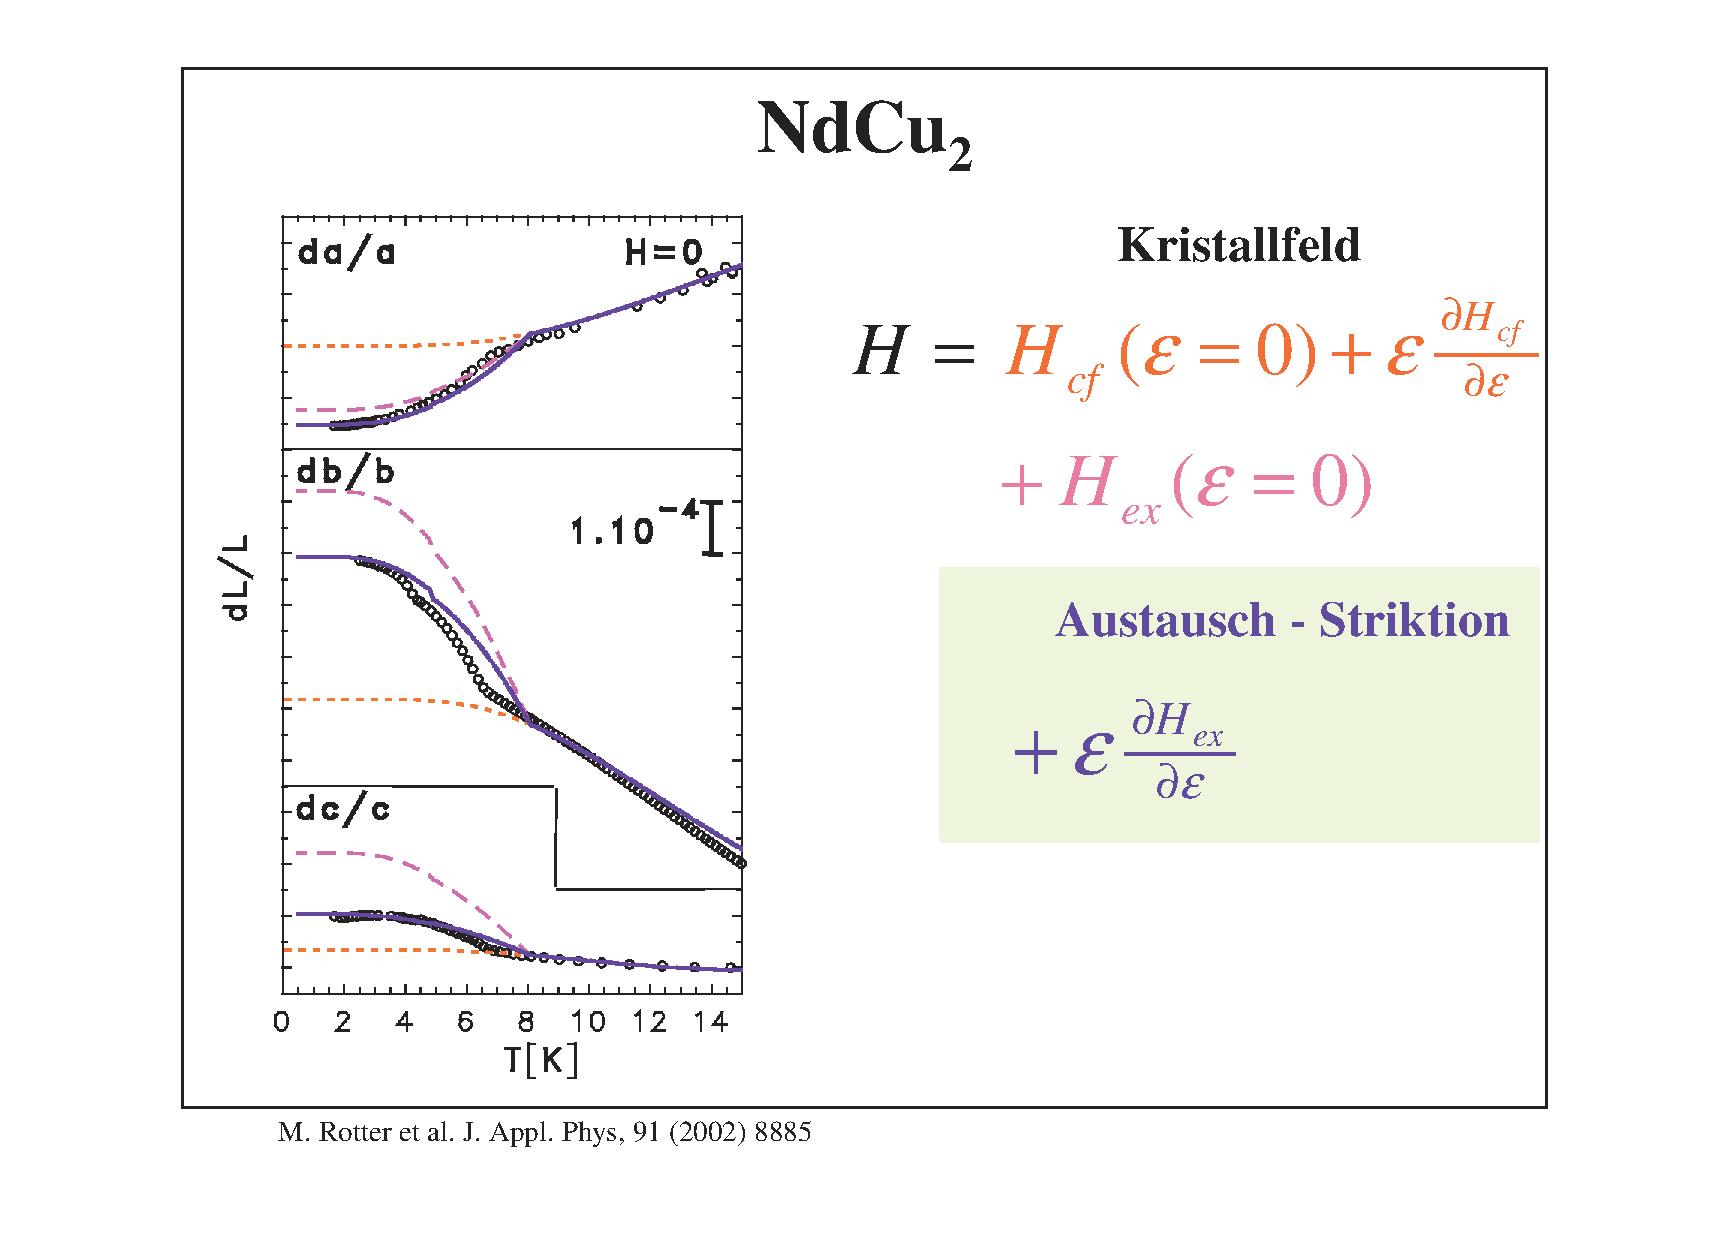
\includegraphics[angle=0, width=0.8\textwidth]{figsrc/magnetostriction_ndcu2.eps}
\end{center}
\caption{Calculated spontaneous magnetostriction of NdCu$_2$.}
\label{magnetostrictiongraphic}
\end{figure}

\begin{description}
\item [\prg mcphas.qvc]    the set of test q-vectors used for calculation of free energy.
                           Components of these q vectors refer to the reciprocal lattice $\vec a^*,\vec b^*,\vec c^*$.
\item [\prg mcphas.phs]    spin-configuration table of different types of spin-configurations. 
                            Note, in case of non-orthogonal axes the convention in these tables 
                            is $mb||\vec b$, $mc||(\vec a \times \vec b)$ and $ma$ perpendicular to $mb$ and $mc$.

                           {\em Note}: 
                           there is no natural criteria for deciding, if one spin-configuration is
			   different from another one. Therefore the list of ''different''
			   spin-configurations is dependent on the meaning of ''different''.
			   
			   The program {\prg McPhase} decides whether a spin-configuration is
			   different from another by a simple criteria, namely by the
			   angle between the spins. Comparing two spin configurations it calculates
			   the angle between corresponding spins and if for one spin the
			   angle is not small, the configuration is treated as a different
			   configuration. Therefore for example a ferromagnet with moments
			   in $a$ has a different spin configuration than a ferromagnet with
			   moments in $b$ direction. 
\item [\prg mcphas.sps]    $T-H$ dependence of spin-configuration. The spin configurations stored in this
                           file may be displayed using the program {\prg spins\index{spins}}, an example is given
			   in figure~\ref{spingraphic}.
                            Note, in case of non-orthogonal axes the convention for applied field $Ha, Hb,Hc$ and
                            also for the moment components $ma, mb, mc$ in these tables 
                            is $mb||\vec b$, $mc||(\vec a \times \vec b)$ and $ma$ perpendicular to $mb$ and $mc$.

\item [\prg mcphas.mf]     $T-H$ dependence of exchange field configuration, stored as $g_J \mu_B H_{xc}(i)$(unit is in meV)
                            for i=1,2,...,number of spins in magnetic unit cell.
                            Note, in case of non-orthogonal axes the convention for applied field $Ha, Hb,Hc$ and
                            also for the mean field components in these tables 
                            is $Hb||\vec b$, $Hc||(\vec a \times \vec b)$ and $Ha$ perpendicular to $Hb$ and $Hc$.
\item [\prg mcphas.fum]    free energy, magnetic energy (the derivative with respect to temperature gives the specific %%@
heat),
                           magnetisation data and (if cfield is used with higher order interactions)
                           expectation values of the Stevens Operators $<O_l^m>$ . As an example for the information
			   contained in this file the calculated magnetisation and magnetostriction of NdCu$_2$ is shown in
			   figures~\ref{magnetization} and ~\ref{magnetizationgraphic}.
                            Note, in case of non-orthogonal axes the convention for applied field $Ha, Hb,Hc$ and
                            also for the magnetisation components $ma,mb,mc$ in these tables 
                            is $Hb||\vec b$, $Hc||(\vec a \times \vec b)$ and $Ha$ perpendicular to $Hb$ and $Hc$.

\item [\prg mcphas1.j1 .j1 .j2 ...] 
               spin-spin correlation functions for sub-lattice 1 neighbour 1 2 ...
	       (linear combination is proportional to magnetostriction)
	       The spin-spin correlation functions for neighbour $k$ are defined by
	       the following sum of dyadic products:

	       \begin{equation}
	        \frac{1}{n}\sum_{s=1}^n <{\mbf J}^s> \times  <{\mbf J}^{s+k}>
	       \end{equation}
	       with $n$ being the number of moments in the magnetic unit cell.
	       Single ion and two-ion magnetostriction can be calculated using the $<O_l^m>$ and the
	       spin-spin correlation functions. As an example the magnetostriction analysis of
	       NdCu$_2$ is shown in figure~\ref{magnetostrictiongraphic}. For details 
             please refer to~\cite{rotter02-8885}.
                            Note, in case of non-orthogonal axes the convention for applied field $Ha, Hb,Hc$ and
                            also for the moment components in these tables 
                            is $Hb||\vec b$, $Hc||(\vec a \times \vec b)$ and $Ha$ perpendicular to $Hb$ and $Hc$.
\item [\prg mcphas.xyt]    phase diagram as x,y,T, H, phase-number j according to spin-configuration table
               given in mcphas.phs, a periodicity key, nettomoments <J>.
 Figure~\ref{phasediagramgraphic}
	       shows the phase diagram of NdCu$_2$ for magnetic fields parallel to the orthorhombic $b$-direction.
                            Note, in case of non-orthogonal axes the convention for applied field $Ha, Hb,Hc$ 
                             in these tables 
                            is $Hb||\vec b$, $Hc||(\vec a \times \vec b)$ and $Ha$ perpendicular to $Hb$ and $Hc$.
\item [\prg mcphas.hkl]    calculated (unpolarised) neutron diffraction data (the calculated magnetic intensities
    correspond to the magnetic structure + Polarisation factor. The
    Lorentz-factor , magnetic form factor and  instrumental corrections are not calculated.)
 As an example figure~\ref{neutintgraphic}
    shows the calculated temperature dependence of magnetic amplitudes for NdCu$_2$.
                           $h,k,l$ refer to the reciprocal lattice $\vec a^*,\vec b^*,\vec c^*$.
                            Note, in case of non-orthogonal axes the convention for applied field $Ha, Hb,Hc$ 
                             in these tables 
                            is $Hb||\vec b$, $Hc||(\vec a \times \vec b)$ and $Ha$ perpendicular to $Hb$ and $Hc$.
    
\item [\prg mcphasa.hkl]    Fourier Transform of the $a$-component of the magnetic Moments.
                           $h,k,l$ refer to the reciprocal lattice $\vec a^*,\vec b^*,\vec c^*$.
                            Note, in case of non-orthogonal axes the convention for applied field $Ha, Hb,Hc$ and
                            the magnetic moment component in these tables 
                            is $Hb||\vec b$, $Hc||(\vec a \times \vec b)$ and $Ha$ perpendicular to $Hb$ and $Hc$.
\item [\prg mcphasb.hkl]    Fourier Transform of the $b$-component of the magnetic Moments.
                           $h,k,l$ refer to the reciprocal lattice $\vec a^*,\vec b^*,\vec c^*$.
                            Note, in case of non-orthogonal axes the convention for applied field $Ha, Hb,Hc$ and
                            the magnetic moment component in these tables 
                            is $Hb||\vec b$, $Hc||(\vec a \times \vec b)$ and $Ha$ perpendicular to $Hb$ and $Hc$.
\item [\prg mcphasc.hkl]    Fourier Transform of the $c$-component of the magnetic Moments.
                           $h,k,l$ refer to the reciprocal lattice $\vec a^*,\vec b^*,\vec c^*$.
                            Note, in case of non-orthogonal axes the convention for applied field $Ha, Hb,Hc$ and
                            the magnetic moment component in these tables 
                            is $Hb||\vec b$, $Hc||(\vec a \times \vec b)$ and $Ha$ perpendicular to $Hb$ and $Hc$.
\end{description} 

\vspace{1cm}
{\em Exercises:}
\begin{itemize}
\item Look at the output files of {\prg McPhase}  in the directory
{\prg examples/ndcu2b\_new/results}.  At which magnetic field
the ferromagnetically aligned state is achieved (at $T=$2~K)?
\item
What is the propagation vector in the different antiferromagnetic phases at $T=$2~K ?
\end{itemize}


Note, in case of non-orthogonal axes the convention 
is $mb||\vec b$, $mc||(\vec a \times \vec b)$ and $ma$ perpendicular to $mb$ and $mc$.

\subsubsection{subdirectory {\prg ./results} - directory where calculated data is stored}

In order to be able to save the results of a calculation the directory {\prg ./results} has to
exist. Mind that all files in this directory will be overwritten without warning. 

\subsubsection{subdirectory {\prg ./fit} - experimental data for fit (optional) } 

In order that {\prg McPhase} can calculate the standard deviation between
 experimental data and the results of the simulation, some experimental data
 can be given in the subdirectory {\prg ./fit}. The filenames and the data-format
 are the same as the output files of {\prg McPhas}, e.g. {\prg mcphas.fum}, {\prg mcphas.hkl}
 etc. {\prg McPhase} looks into the directory {\prg ./fit} and if it finds any
 of these files, the standard deviation is increased correspondingly. 

What measurement data can be used to calculate a standard deviation ?

\begin{description}
\item[{\prg mcphas.fum}] if given in column 11, 12, 13 in {\prg ./fit/mcphas.fum} the
            magnetisation in the $a$, $b$ and $c$ direction is used for calculation
	    of the standard deviation sta. The standard deviation is calculated
	    as ${\rm sta}=\sum_{\rm data points i} ({\mbf m}_i^{calc}-{\mbf m}_i^{meas})^2$.
	    All three components of the magnetic moment have to be given and are used.

\end{description}

Note that the measured data has to be given in those (H-T) points which are 
calculated by mcphas\index{mcphas} in order to be used by the program to increase {\prg sta}.
It is usually most effective to fit only few data points, because a large set
of data points will not improve the quality of the fit and only require a large
amount of calculation time.



\subsection{Starting a simulation}
\label{start}

To start the simulation goto the directory containing the
input files {\prg mcphas.ini, mcphas.j, etc. } and type

\begin{description}
\item[\prg mcphas] to run the program generating stepwise $H-T$ values 
              in a loop given by {\prg mcphas.ini\index{mcphas.ini}} (you can also press the
              symbol in the {\prg McPhase - Explorer} window).
\item[\prg mcphas\index{mcphas} [file]]  to run the program with an input file --   
             {\prg file} contains T ha hb hc values to be calculated 
             if [file] is not given, xmin xmax xstep (xT xHa xHb xHc)
             ymin ymax ystep (yT yHa yHb yHc) is read from file {\prg mcphas.ini\index{mcphas.ini}}
	     and phase diagram is calculated
\item[\prg mcphas\index{mcphas} -h]  to  print help and version of {\prg McPhas}.
\item[\prg mcphas\index{mcphas} -stamax 14]  end mcphas\index{mcphas} if standard deviation exceeds 14.
\item[\prg mcphas\index{mcphas} -a] avoid overwriting output files in results, append new results to existing files
\item[\prg mcphas\index{mcphas} -v]  to  enable verbose mode with lots of messages of {\prg McPhas}. Specifically
the verbose mode enables the following features:
  \begin{itemize}
			          \item more information is printed out, 
			          \item the q-vectors file {\prg ./results/mcphas.qvc} will contain 
				    the explicit spin configurations
			          \item the display\index{display} on screen (ghostview window using 
				     {\prg ./results/.sps.eps}) will be updated not only 
				    when a H-T point has been finished but always 
				    when a structure with smaller free energy 
				    has been stabilised
  \end{itemize}
\item[\prg mcphasit\index{mcphas}] to start mcphase in commandline mode without opening any window
\end{description}

\vspace{1cm}
{\em Exercises:}
\begin{itemize}
\item Look at the input files for {\prg McPhase} given in the directory
{\prg examples/ndcu2b\_new}.  How many atoms are contained in the crystallographic basis ?
\item
Start the simulation by typing the command {\prg mcphas}.
\end{itemize}



\subsection{Options for a running simulation}
... when the program is running, the options in the main window
can be changed. Pressing ''displayall'' displays the current spin-configuration
at each iteration step. Pressing ''log fe vs Q'' appends free energy vs Q
data to {\prg mcphas.log} for every ($T-H$) point.


The file {\prg ./results/.spins.eps} is used to show the information about the currently calculated
spin structure on the screen using the postscript file viewer ghostview.

The file {\prg ./results/.mcphas.fum} contains the information of the magnetisation curve
which is currently calculated. This information is automatically displayed on the screen.


The program {\prg display} (see section \ref{display}) can be used 
for the online display\index{display} of any other
curve(s).


\subsection{Output Files - {\prg mcphas.qvc,phs,sps,mf,fum,j1...,xyt,hkl} }\label{outputfiles}
 (in directory ./results/ after a simulation run) 

\begin{figure}[htb]%h=here, t=top, b=bottom, p=separate figure page
\begin{center}\leavevmode
\includegraphics[angle=0, width=0.3\textwidth]{figsrc/magnetization_ndcu2.ps}
\end{center}
\caption{Calculated magnetisation of NdCu$_2$ for field parallel to the orthorhombic $b$-direction.}
\label{magnetization}
\end{figure}

\begin{figure}[htb]%h=here, t=top, b=bottom, p=separate figure page
\begin{center}\leavevmode
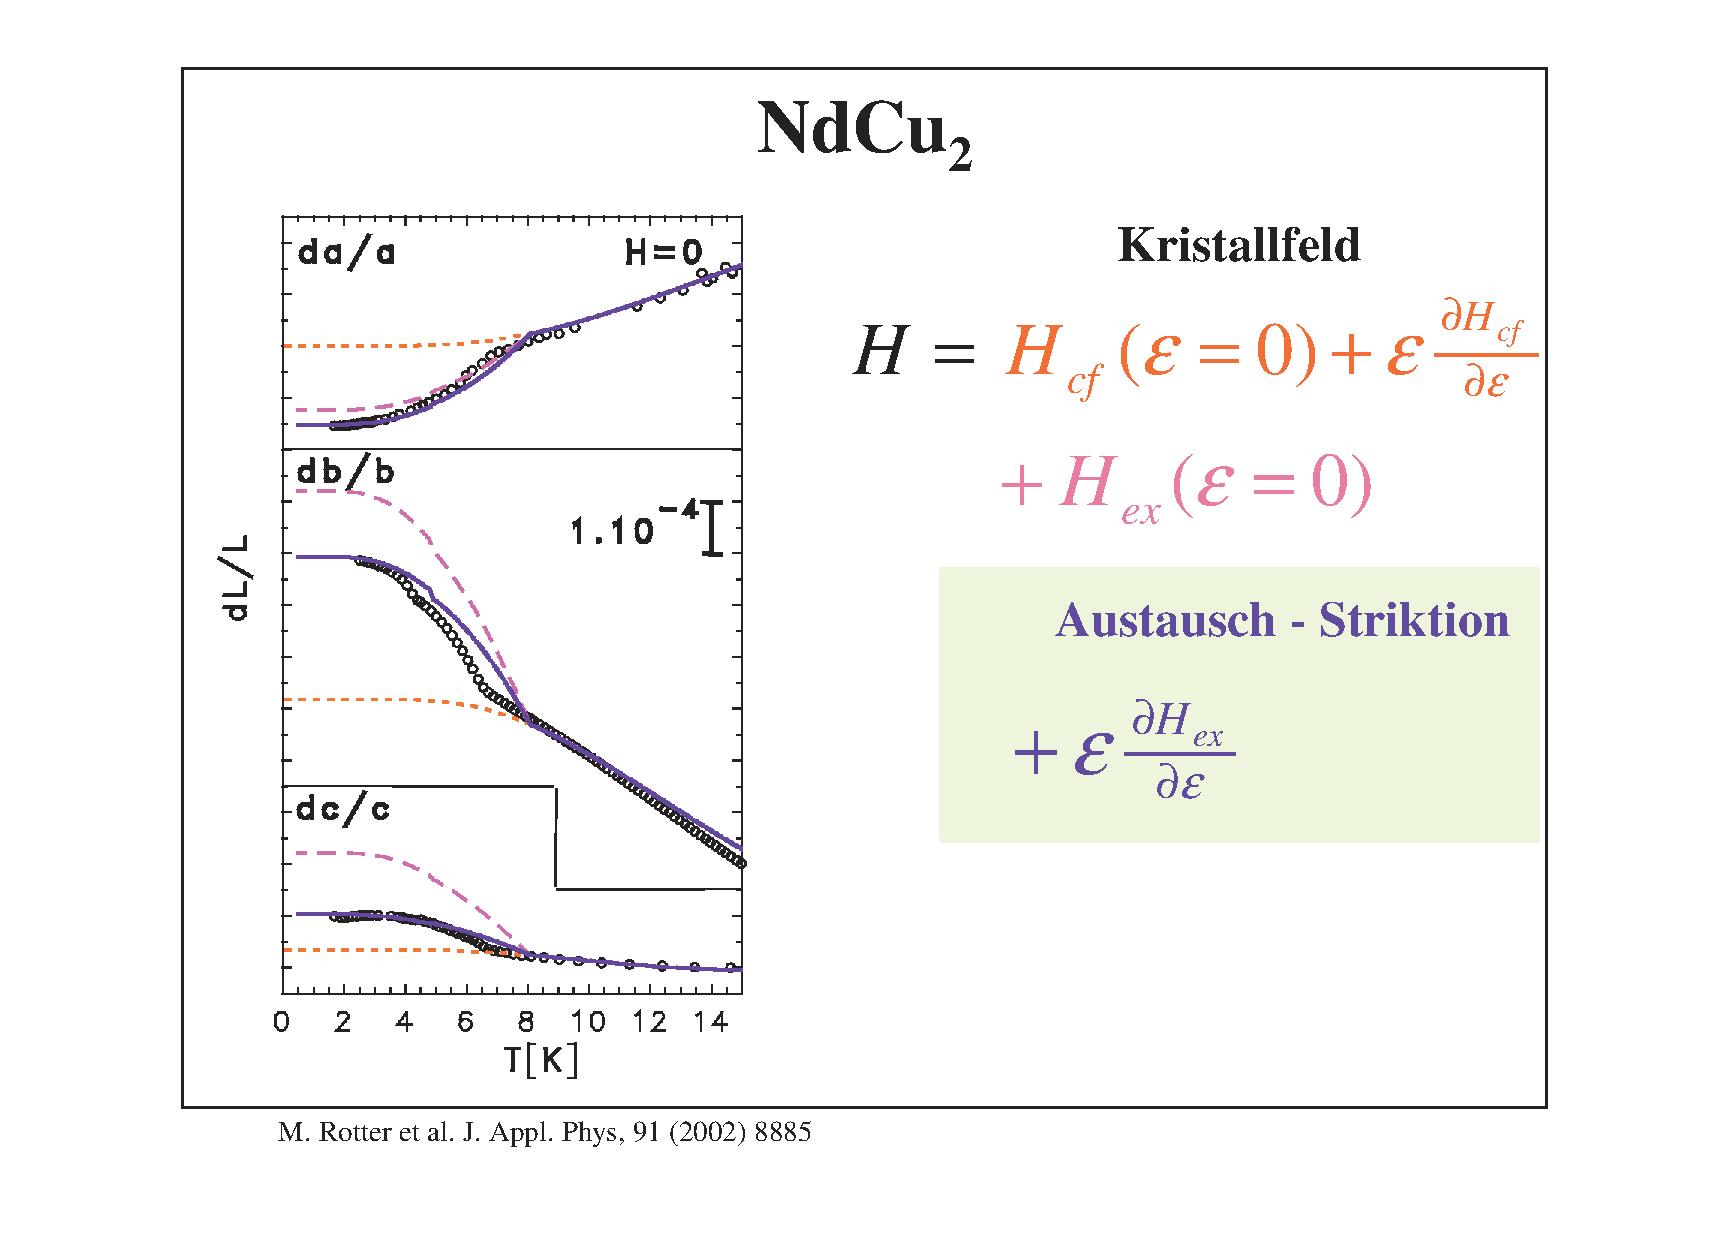
\includegraphics[angle=0, width=0.8\textwidth]{figsrc/magnetostriction_ndcu2.eps}
\end{center}
\caption{Calculated spontaneous magnetostriction of NdCu$_2$.}
\label{magnetostrictiongraphic}
\end{figure}

\begin{description}
\item [\prg mcphas.qvc]    the set of test q-vectors used for calculation of free energy.
                           Components of these q vectors refer to the reciprocal lattice $\vec a^*,\vec b^*,\vec c^*$.
\item [\prg mcphas.phs]    spin-configuration table of different types of spin-configurations. 
                            Note, in case of non-orthogonal axes the convention in these tables 
                            is $mb||\vec b$, $mc||(\vec a \times \vec b)$ and $ma$ perpendicular to $mb$ and $mc$.

                           {\em Note}: 
                           there is no natural criteria for deciding, if one spin-configuration is
			   different from another one. Therefore the list of ''different''
			   spin-configurations is dependent on the meaning of ''different''.
			   
			   The program {\prg McPhase} decides whether a spin-configuration is
			   different from another by a simple criteria, namely by the
			   angle between the spins. Comparing two spin configurations it calculates
			   the angle between corresponding spins and if for one spin the
			   angle is not small, the configuration is treated as a different
			   configuration. Therefore for example a ferromagnet with moments
			   in $a$ has a different spin configuration than a ferromagnet with
			   moments in $b$ direction. 
\item [\prg mcphas.sps]    $T-H$ dependence of spin-configuration. The spin configurations stored in this
                           file may be displayed using the program {\prg spins\index{spins}}, an example is given
			   in figure~\ref{spingraphic}.
                            Note, in case of non-orthogonal axes the convention for applied field $Ha, Hb,Hc$ and
                            also for the moment components $ma, mb, mc$ in these tables 
                            is $mb||\vec b$, $mc||(\vec a \times \vec b)$ and $ma$ perpendicular to $mb$ and $mc$.

\item [\prg mcphas.mf]     $T-H$ dependence of exchange field configuration, stored as $g_J \mu_B H_{xc}(i)$(unit is in meV)
                            for i=1,2,...,number of spins in magnetic unit cell.
                            Note, in case of non-orthogonal axes the convention for applied field $Ha, Hb,Hc$ and
                            also for the mean field components in these tables 
                            is $Hb||\vec b$, $Hc||(\vec a \times \vec b)$ and $Ha$ perpendicular to $Hb$ and $Hc$.
\item [\prg mcphas.fum]    free energy, magnetic energy (the derivative with respect to temperature gives the specific %%@
heat),
                           magnetisation data and (if cfield is used with higher order interactions)
                           expectation values of the Stevens Operators $<O_l^m>$ . As an example for the information
			   contained in this file the calculated magnetisation and magnetostriction of NdCu$_2$ is shown in
			   figures~\ref{magnetization} and ~\ref{magnetizationgraphic}.
                            Note, in case of non-orthogonal axes the convention for applied field $Ha, Hb,Hc$ and
                            also for the magnetisation components $ma,mb,mc$ in these tables 
                            is $Hb||\vec b$, $Hc||(\vec a \times \vec b)$ and $Ha$ perpendicular to $Hb$ and $Hc$.

\item [\prg mcphas1.j1 .j1 .j2 ...] 
               spin-spin correlation functions for sub-lattice 1 neighbour 1 2 ...
	       (linear combination is proportional to magnetostriction)
	       The spin-spin correlation functions for neighbour $k$ are defined by
	       the following sum of dyadic products:

	       \begin{equation}
	        \frac{1}{n}\sum_{s=1}^n <{\mbf J}^s> \times  <{\mbf J}^{s+k}>
	       \end{equation}
	       with $n$ being the number of moments in the magnetic unit cell.
	       Single ion and two-ion magnetostriction can be calculated using the $<O_l^m>$ and the
	       spin-spin correlation functions. As an example the magnetostriction analysis of
	       NdCu$_2$ is shown in figure~\ref{magnetostrictiongraphic}. For details 
             please refer to~\cite{rotter02-8885}.
                            Note, in case of non-orthogonal axes the convention for applied field $Ha, Hb,Hc$ and
                            also for the moment components in these tables 
                            is $Hb||\vec b$, $Hc||(\vec a \times \vec b)$ and $Ha$ perpendicular to $Hb$ and $Hc$.
\item [\prg mcphas.xyt]    phase diagram as x,y,T, H, phase-number j according to spin-configuration table
               given in mcphas.phs, a periodicity key, nettomoments <J>.
 Figure~\ref{phasediagramgraphic}
	       shows the phase diagram of NdCu$_2$ for magnetic fields parallel to the orthorhombic $b$-direction.
                            Note, in case of non-orthogonal axes the convention for applied field $Ha, Hb,Hc$ 
                             in these tables 
                            is $Hb||\vec b$, $Hc||(\vec a \times \vec b)$ and $Ha$ perpendicular to $Hb$ and $Hc$.
\item [\prg mcphas.hkl]    calculated (unpolarised) neutron diffraction data (the calculated magnetic intensities
    correspond to the magnetic structure + Polarisation factor. The
    Lorentz-factor , magnetic form factor and  instrumental corrections are not calculated.)
 As an example figure~\ref{neutintgraphic}
    shows the calculated temperature dependence of magnetic amplitudes for NdCu$_2$.
                           $h,k,l$ refer to the reciprocal lattice $\vec a^*,\vec b^*,\vec c^*$.
                            Note, in case of non-orthogonal axes the convention for applied field $Ha, Hb,Hc$ 
                             in these tables 
                            is $Hb||\vec b$, $Hc||(\vec a \times \vec b)$ and $Ha$ perpendicular to $Hb$ and $Hc$.
    
\item [\prg mcphasa.hkl]    Fourier Transform of the $a$-component of the magnetic Moments.
                           $h,k,l$ refer to the reciprocal lattice $\vec a^*,\vec b^*,\vec c^*$.
                            Note, in case of non-orthogonal axes the convention for applied field $Ha, Hb,Hc$ and
                            the magnetic moment component in these tables 
                            is $Hb||\vec b$, $Hc||(\vec a \times \vec b)$ and $Ha$ perpendicular to $Hb$ and $Hc$.
\item [\prg mcphasb.hkl]    Fourier Transform of the $b$-component of the magnetic Moments.
                           $h,k,l$ refer to the reciprocal lattice $\vec a^*,\vec b^*,\vec c^*$.
                            Note, in case of non-orthogonal axes the convention for applied field $Ha, Hb,Hc$ and
                            the magnetic moment component in these tables 
                            is $Hb||\vec b$, $Hc||(\vec a \times \vec b)$ and $Ha$ perpendicular to $Hb$ and $Hc$.
\item [\prg mcphasc.hkl]    Fourier Transform of the $c$-component of the magnetic Moments.
                           $h,k,l$ refer to the reciprocal lattice $\vec a^*,\vec b^*,\vec c^*$.
                            Note, in case of non-orthogonal axes the convention for applied field $Ha, Hb,Hc$ and
                            the magnetic moment component in these tables 
                            is $Hb||\vec b$, $Hc||(\vec a \times \vec b)$ and $Ha$ perpendicular to $Hb$ and $Hc$.
\end{description} 

\vspace{1cm}
{\em Exercises:}
\begin{itemize}
\item Look at the output files of {\prg McPhase}  in the directory
{\prg examples/ndcu2b\_new/results}.  At which magnetic field
the ferromagnetically aligned state is achieved (at $T=$2~K)?
\item
What is the propagation vector in the different antiferromagnetic phases at $T=$2~K ?
\end{itemize}


Note, in case of non-orthogonal axes the convention 
is $mb||\vec b$, $mc||(\vec a \times \vec b)$ and $ma$ perpendicular to $mb$ and $mc$.

\subsubsection{subdirectory {\prg ./results} - directory where calculated data is stored}

In order to be able to save the results of a calculation the directory {\prg ./results} has to
exist. Mind that all files in this directory will be overwritten without warning. 

\subsubsection{subdirectory {\prg ./fit} - experimental data for fit (optional) } 

In order that {\prg McPhase} can calculate the standard deviation between
 experimental data and the results of the simulation, some experimental data
 can be given in the subdirectory {\prg ./fit}. The filenames and the data-format
 are the same as the output files of {\prg McPhas}, e.g. {\prg mcphas.fum}, {\prg mcphas.hkl}
 etc. {\prg McPhase} looks into the directory {\prg ./fit} and if it finds any
 of these files, the standard deviation is increased correspondingly. 

What measurement data can be used to calculate a standard deviation ?

\begin{description}
\item[{\prg mcphas.fum}] if given in column 11, 12, 13 in {\prg ./fit/mcphas.fum} the
            magnetisation in the $a$, $b$ and $c$ direction is used for calculation
	    of the standard deviation sta. The standard deviation is calculated
	    as ${\rm sta}=\sum_{\rm data points i} ({\mbf m}_i^{calc}-{\mbf m}_i^{meas})^2$.
	    All three components of the magnetic moment have to be given and are used.

\end{description}

Note that the measured data has to be given in those (H-T) points which are 
calculated by mcphas\index{mcphas} in order to be used by the program to increase {\prg sta}.
It is usually most effective to fit only few data points, because a large set
of data points will not improve the quality of the fit and only require a large
amount of calculation time.



\subsection{Starting a simulation}
\label{start}

To start the simulation goto the directory containing the
input files {\prg mcphas.ini, mcphas.j, etc. } and type

\begin{description}
\item[\prg mcphas] to run the program generating stepwise $H-T$ values 
              in a loop given by {\prg mcphas.ini\index{mcphas.ini}} (you can also press the
              symbol in the {\prg McPhase - Explorer} window).
\item[\prg mcphas\index{mcphas} [file]]  to run the program with an input file --   
             {\prg file} contains T ha hb hc values to be calculated 
             if [file] is not given, xmin xmax xstep (xT xHa xHb xHc)
             ymin ymax ystep (yT yHa yHb yHc) is read from file {\prg mcphas.ini\index{mcphas.ini}}
	     and phase diagram is calculated
\item[\prg mcphas\index{mcphas} -h]  to  print help and version of {\prg McPhas}.
\item[\prg mcphas\index{mcphas} -stamax 14]  end mcphas\index{mcphas} if standard deviation exceeds 14.
\item[\prg mcphas\index{mcphas} -a] avoid overwriting output files in results, append new results to existing files
\item[\prg mcphas\index{mcphas} -v]  to  enable verbose mode with lots of messages of {\prg McPhas}. Specifically
the verbose mode enables the following features:
  \begin{itemize}
			          \item more information is printed out, 
			          \item the q-vectors file {\prg ./results/mcphas.qvc} will contain 
				    the explicit spin configurations
			          \item the display\index{display} on screen (ghostview window using 
				     {\prg ./results/.sps.eps}) will be updated not only 
				    when a H-T point has been finished but always 
				    when a structure with smaller free energy 
				    has been stabilised
  \end{itemize}
\item[\prg mcphasit\index{mcphas}] to start mcphase in commandline mode without opening any window
\end{description}

\vspace{1cm}
{\em Exercises:}
\begin{itemize}
\item Look at the input files for {\prg McPhase} given in the directory
{\prg examples/ndcu2b\_new}.  How many atoms are contained in the crystallographic basis ?
\item
Start the simulation by typing the command {\prg mcphas}.
\end{itemize}



\subsection{Options for a running simulation}
... when the program is running, the options in the main window
can be changed. Pressing ''displayall'' displays the current spin-configuration
at each iteration step. Pressing ''log fe vs Q'' appends free energy vs Q
data to {\prg mcphas.log} for every ($T-H$) point.


The file {\prg ./results/.spins.eps} is used to show the information about the currently calculated
spin structure on the screen using the postscript file viewer ghostview.

The file {\prg ./results/.mcphas.fum} contains the information of the magnetisation curve
which is currently calculated. This information is automatically displayed on the screen.


The program {\prg display} (see section \ref{display}) can be used 
for the online display\index{display} of any other
curve(s).


\subsection{Output Files - {\prg mcphas.qvc,phs,sps,mf,fum,j1...,xyt,hkl} }\label{outputfiles}
 (in directory ./results/ after a simulation run) 

\begin{figure}[htb]%h=here, t=top, b=bottom, p=separate figure page
\begin{center}\leavevmode
\includegraphics[angle=0, width=0.3\textwidth]{figsrc/magnetization_ndcu2.ps}
\end{center}
\caption{Calculated magnetisation of NdCu$_2$ for field parallel to the orthorhombic $b$-direction.}
\label{magnetization}
\end{figure}

\begin{figure}[htb]%h=here, t=top, b=bottom, p=separate figure page
\begin{center}\leavevmode
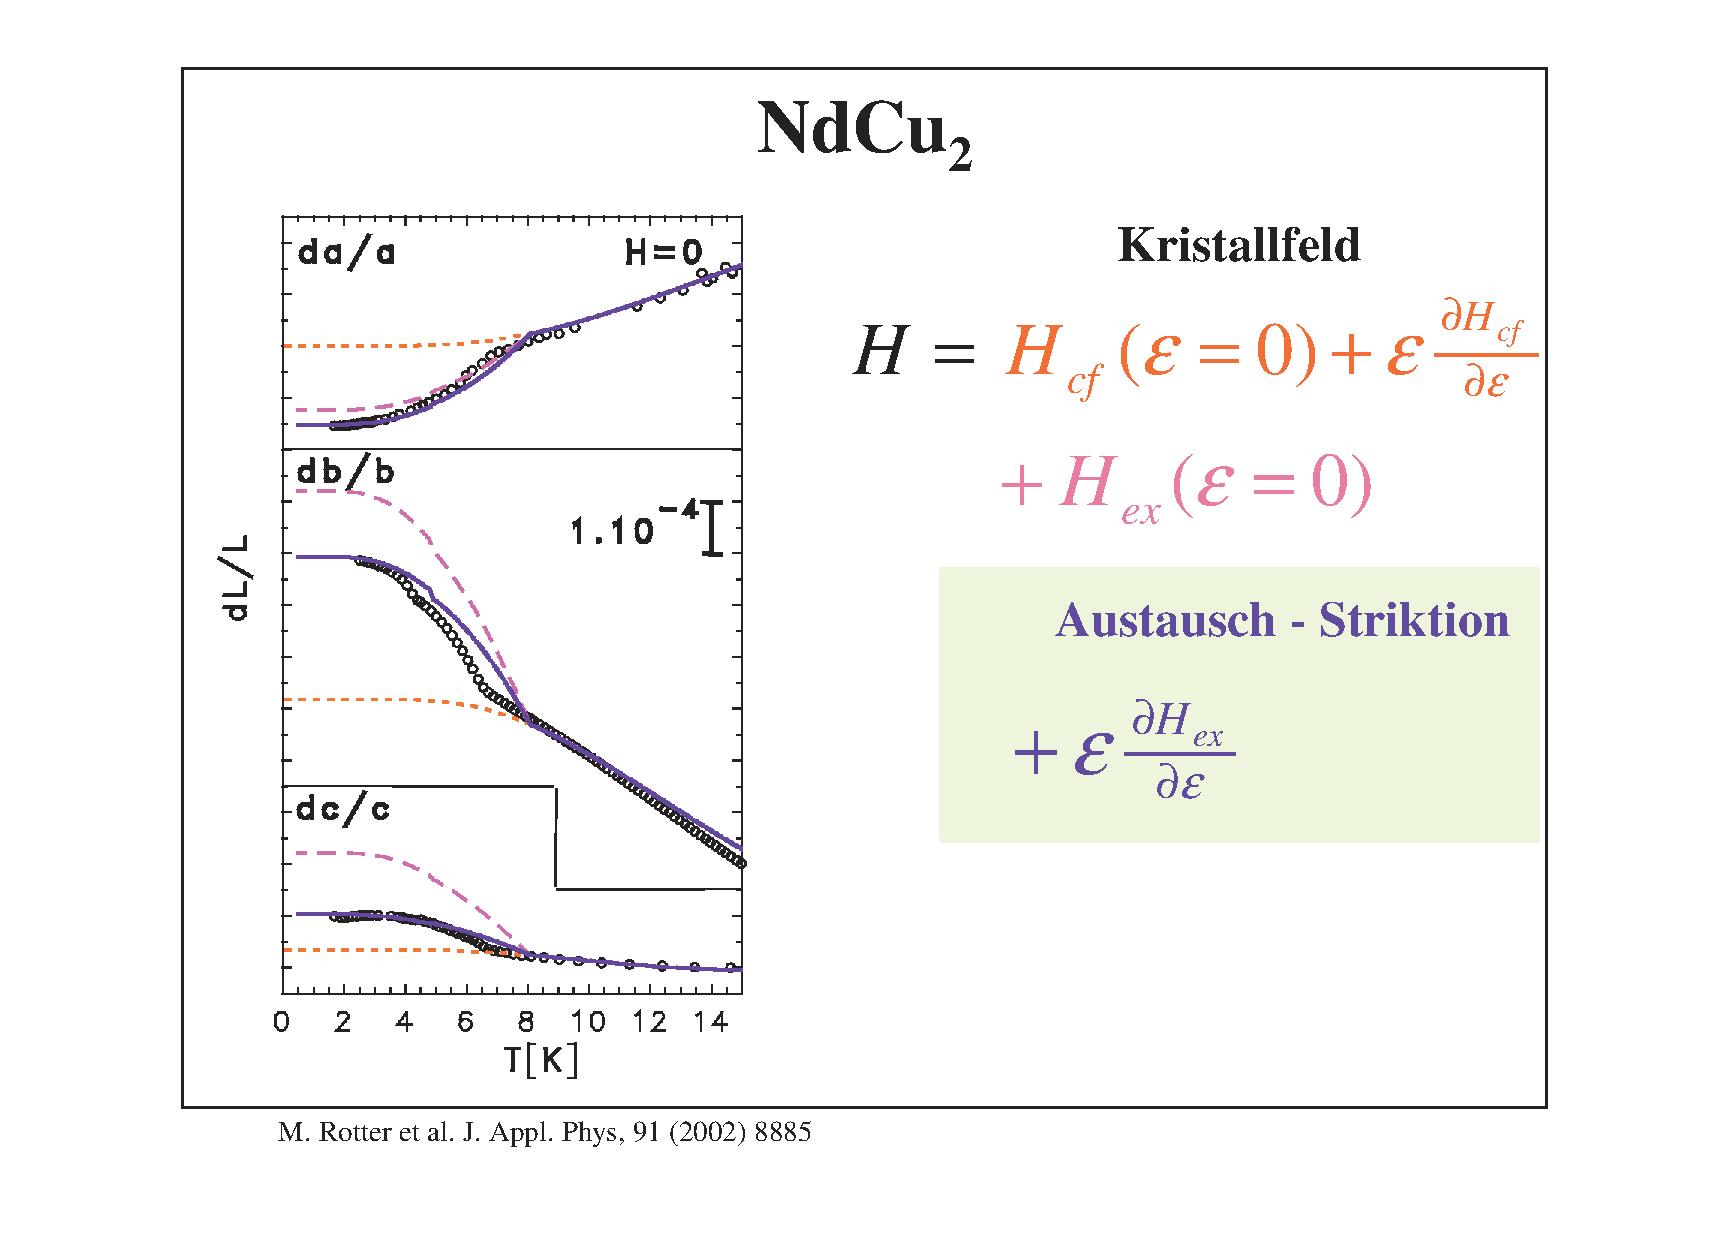
\includegraphics[angle=0, width=0.8\textwidth]{figsrc/magnetostriction_ndcu2.eps}
\end{center}
\caption{Calculated spontaneous magnetostriction of NdCu$_2$.}
\label{magnetostrictiongraphic}
\end{figure}

\begin{description}
\item [\prg mcphas.qvc]    the set of test q-vectors used for calculation of free energy.
                           Components of these q vectors refer to the reciprocal lattice $\vec a^*,\vec b^*,\vec c^*$.
\item [\prg mcphas.phs]    spin-configuration table of different types of spin-configurations. 
                            Note, in case of non-orthogonal axes the convention in these tables 
                            is $mb||\vec b$, $mc||(\vec a \times \vec b)$ and $ma$ perpendicular to $mb$ and $mc$.

                           {\em Note}: 
                           there is no natural criteria for deciding, if one spin-configuration is
			   different from another one. Therefore the list of ''different''
			   spin-configurations is dependent on the meaning of ''different''.
			   
			   The program {\prg McPhase} decides whether a spin-configuration is
			   different from another by a simple criteria, namely by the
			   angle between the spins. Comparing two spin configurations it calculates
			   the angle between corresponding spins and if for one spin the
			   angle is not small, the configuration is treated as a different
			   configuration. Therefore for example a ferromagnet with moments
			   in $a$ has a different spin configuration than a ferromagnet with
			   moments in $b$ direction. 
\item [\prg mcphas.sps]    $T-H$ dependence of spin-configuration. The spin configurations stored in this
                           file may be displayed using the program {\prg spins\index{spins}}, an example is given
			   in figure~\ref{spingraphic}.
                            Note, in case of non-orthogonal axes the convention for applied field $Ha, Hb,Hc$ and
                            also for the moment components $ma, mb, mc$ in these tables 
                            is $mb||\vec b$, $mc||(\vec a \times \vec b)$ and $ma$ perpendicular to $mb$ and $mc$.

\item [\prg mcphas.mf]     $T-H$ dependence of exchange field configuration, stored as $g_J \mu_B H_{xc}(i)$(unit is in meV)
                            for i=1,2,...,number of spins in magnetic unit cell.
                            Note, in case of non-orthogonal axes the convention for applied field $Ha, Hb,Hc$ and
                            also for the mean field components in these tables 
                            is $Hb||\vec b$, $Hc||(\vec a \times \vec b)$ and $Ha$ perpendicular to $Hb$ and $Hc$.
\item [\prg mcphas.fum]    free energy, magnetic energy (the derivative with respect to temperature gives the specific %%@
heat),
                           magnetisation data and (if cfield is used with higher order interactions)
                           expectation values of the Stevens Operators $<O_l^m>$ . As an example for the information
			   contained in this file the calculated magnetisation and magnetostriction of NdCu$_2$ is shown in
			   figures~\ref{magnetization} and ~\ref{magnetizationgraphic}.
                            Note, in case of non-orthogonal axes the convention for applied field $Ha, Hb,Hc$ and
                            also for the magnetisation components $ma,mb,mc$ in these tables 
                            is $Hb||\vec b$, $Hc||(\vec a \times \vec b)$ and $Ha$ perpendicular to $Hb$ and $Hc$.

\item [\prg mcphas1.j1 .j1 .j2 ...] 
               spin-spin correlation functions for sub-lattice 1 neighbour 1 2 ...
	       (linear combination is proportional to magnetostriction)
	       The spin-spin correlation functions for neighbour $k$ are defined by
	       the following sum of dyadic products:

	       \begin{equation}
	        \frac{1}{n}\sum_{s=1}^n <{\mbf J}^s> \times  <{\mbf J}^{s+k}>
	       \end{equation}
	       with $n$ being the number of moments in the magnetic unit cell.
	       Single ion and two-ion magnetostriction can be calculated using the $<O_l^m>$ and the
	       spin-spin correlation functions. As an example the magnetostriction analysis of
	       NdCu$_2$ is shown in figure~\ref{magnetostrictiongraphic}. For details 
             please refer to~\cite{rotter02-8885}.
                            Note, in case of non-orthogonal axes the convention for applied field $Ha, Hb,Hc$ and
                            also for the moment components in these tables 
                            is $Hb||\vec b$, $Hc||(\vec a \times \vec b)$ and $Ha$ perpendicular to $Hb$ and $Hc$.
\item [\prg mcphas.xyt]    phase diagram as x,y,T, H, phase-number j according to spin-configuration table
               given in mcphas.phs, a periodicity key, nettomoments <J>.
 Figure~\ref{phasediagramgraphic}
	       shows the phase diagram of NdCu$_2$ for magnetic fields parallel to the orthorhombic $b$-direction.
                            Note, in case of non-orthogonal axes the convention for applied field $Ha, Hb,Hc$ 
                             in these tables 
                            is $Hb||\vec b$, $Hc||(\vec a \times \vec b)$ and $Ha$ perpendicular to $Hb$ and $Hc$.
\item [\prg mcphas.hkl]    calculated (unpolarised) neutron diffraction data (the calculated magnetic intensities
    correspond to the magnetic structure + Polarisation factor. The
    Lorentz-factor , magnetic form factor and  instrumental corrections are not calculated.)
 As an example figure~\ref{neutintgraphic}
    shows the calculated temperature dependence of magnetic amplitudes for NdCu$_2$.
                           $h,k,l$ refer to the reciprocal lattice $\vec a^*,\vec b^*,\vec c^*$.
                            Note, in case of non-orthogonal axes the convention for applied field $Ha, Hb,Hc$ 
                             in these tables 
                            is $Hb||\vec b$, $Hc||(\vec a \times \vec b)$ and $Ha$ perpendicular to $Hb$ and $Hc$.
    
\item [\prg mcphasa.hkl]    Fourier Transform of the $a$-component of the magnetic Moments.
                           $h,k,l$ refer to the reciprocal lattice $\vec a^*,\vec b^*,\vec c^*$.
                            Note, in case of non-orthogonal axes the convention for applied field $Ha, Hb,Hc$ and
                            the magnetic moment component in these tables 
                            is $Hb||\vec b$, $Hc||(\vec a \times \vec b)$ and $Ha$ perpendicular to $Hb$ and $Hc$.
\item [\prg mcphasb.hkl]    Fourier Transform of the $b$-component of the magnetic Moments.
                           $h,k,l$ refer to the reciprocal lattice $\vec a^*,\vec b^*,\vec c^*$.
                            Note, in case of non-orthogonal axes the convention for applied field $Ha, Hb,Hc$ and
                            the magnetic moment component in these tables 
                            is $Hb||\vec b$, $Hc||(\vec a \times \vec b)$ and $Ha$ perpendicular to $Hb$ and $Hc$.
\item [\prg mcphasc.hkl]    Fourier Transform of the $c$-component of the magnetic Moments.
                           $h,k,l$ refer to the reciprocal lattice $\vec a^*,\vec b^*,\vec c^*$.
                            Note, in case of non-orthogonal axes the convention for applied field $Ha, Hb,Hc$ and
                            the magnetic moment component in these tables 
                            is $Hb||\vec b$, $Hc||(\vec a \times \vec b)$ and $Ha$ perpendicular to $Hb$ and $Hc$.
\end{description} 

\vspace{1cm}
{\em Exercises:}
\begin{itemize}
\item Look at the output files of {\prg McPhase}  in the directory
{\prg examples/ndcu2b\_new/results}.  At which magnetic field
the ferromagnetically aligned state is achieved (at $T=$2~K)?
\item
What is the propagation vector in the different antiferromagnetic phases at $T=$2~K ?
\end{itemize}





\subsubsection{{\prg mcphas.j\index{mcphas.j}} - lattice and exchange parameters}\label{mcphasj}
This file provides the information about 
the crystallographic
 structure and the magnetic exchange interactions.
For every atom in the crystallographic basis there
has to be given the coordinates, the number of neighbours to be considered, the 
Land\'e factor $g_J$, the single ion property filename and  a set of exchange parameters.
If the exchange parameters (and neighbour positions) are not known for your system, you 
can use the program module {\prg makenn\index{makenn}} (see section \ref{addprog}) to generate 
a list of nearest neighbours and
exchange parameters, currently implemented in {\prg makenn\index{makenn}} are dipolar interactions,
exchange interactions via the Bethe-Slater curve or the RKKY model. Note that in order
to use {\prg makenn\index{makenn}} you have to set up a working {\prg mcphas.j\index{mcphas.j}} file, which may or
may not contain neighbours and interactions.

Use program {\prg addj\index{addj}} to add exchange parameter set stored in different 
such {\prg .j} files (see section~\ref{addprog}).



\begin{description}
\item [Line 1,2:] Comment Lines
\item [Line 3:] lattice constants a,b,c and crystal angles alpha, beta, gamma 
\item [Line 4-6:] primitive lattice vectors
\item [Line 7:] Number of atoms in the primitive crystallographic unit cell ({\prg nofatoms})
\item [Line 8:] a comment line with stars
\item [Line 9:] coordinates  ($d_a$,$d_b$,$d_c$) of 1$^{st}$ magnetic ion in the crystallographic unit cell  with
respect to the lattice vectors $\vec a$,$\vec b$,$\vec c$. The number of neighbours of this 
ion, for which interaction constants are given in the interaction table (nofneighbours). 
If {\prg diagonalexchange}
is set to 0 the 9 components of the exchange tensor are given in column 4-12. 
If {\prg diagonalexchange}
 is 1, only 3 components are given (column 4-6).
If {\prg diagonalexchange}
 is 2, specific components of the exchange tensor can be given in columns 4 onwards. The indices of these components
 must be given in the following line (Line 9a below).
The Land\'e factor of the ion (gJ) and the file name of the corresponding single ion
parameter file (cffilename).
\item [Line 9a:]  If {\prg diagonalexchange=2}, then this line gives the indices of the exchange tensor corresponding to 
 the columns 4 onwards. It must have a variable called {\prg indexexchange} followed by a list of names of components of the interaction
 tensor separated by space. E.g.
 \verb|  #! indexexchange= JaJb JbJc  | 
means column 4 gives the the interaction constant between the
 first angular momentum component of the current ion with the second angular momentum component of its neighbour, whilst 
 column 5 has the interaction constant between the second angular momentum component of this ion with the third component of its
 neighbour. Alternatively, pairs of numbers may be given, as in \verb|  #! indexexchange= 1,2 2,3  |
 Additionally another parameter {\prg symmetricexchange} can be set to 1, where the value in each column is also used 
 for the transposed tensor component. Thus \verb|  #! symmetricexchange=1 indexexchange= JaJb  | is the same as \\
 \verb|  #! indexexchange= JaJb JbJa  | where the 4th and 5th column are the same.
\item [Line 10:]  Comment line
\item [Line 11-(10+nofneighbours):] Interaction table for ion number 1.   
Note: the neighbour coordinates (column 1-3) are given with respect to the lattice vectors
$\vec a$,$\vec b$,$\vec c$. The program then calculates from these values the coordinates
with respect to the primitive lattice $\vec r_1$,~$\vec r_2$,~$\vec r_3$.
($ d_a \vec a + d_b \vec b + d_c \vec c = d_1 \vec r_1 + d_2 \vec r_2 + d_3 \vec r_3$).
Column 4,5,6 \dots contain the components of the interaction tensor $\stackrel{=}{\mathcal J}$. 
Note that in case of non-orthogonal axes the 
components of the moments and the interaction tensor $Ja, Jb, Jc, Jaa, Jbb, Jcc, Jab ...$ 
refer to the orthogonal coordinate system
defined with respect to the nonorthogonal lattice $\vec a,\vec b,\vec c$ as
$Jb||\vec b$, $Jc||(\vec a \times \vec b)$ and $Ja$ perpendicular to $Jb$ and $Jc$.
\item [Line (11+nofneighbours) - end:] for each ion in the unit cell line 8 - (10+nofneighbours)
are repeated.
\end{description}


\vspace{0.5cm}

{\small {\bf Information for experienced users:}
\begin{description}
\item[\prg mcphas.jjj:]
format of exchange parameter file, which only needs a reduced set of exchange
parameters in the input file. Using the program {\prg jjj2j} the file can be transformed
to {\prg mcphas.j\index{mcphas.j}} by adding lines for all the equivalent neighbours. The format definition
of {\prg mcphas.jjj} is the same as {\prg mcphas.j\index{mcphas.j}}, however each line denotes several
equivalent neighbour atoms (instead of only one in {\prg mcphas.j\index{mcphas.j}}) according to the
 following rules:
\begin{itemize}
\item If a nonzero coordinate $d_a$ (or $d_b$,$d_c$) in the interaction table
 corresponds to it's value at the nearest
 lattice point of the primitive lattice,
  additional interactions of the same size
with  neighbours with coordinate $-d_a$ (or $-d_b$,$-d_c$, respectively)
are taken into account. This
holds for each of the three coordinates $d_a$,$d_b$ and $d_c$
 resulting in a maximum
number of 8 equivalent neighbours per line in the interaction table.
\item If the value of $d_a$ (or $d_b$,$d_c$) is zero or differs
from it's value at the nearest lattice point of the primitive lattice, it is 
changed to the value at the nearest lattice point and {\bf no} interaction 
with  neighbours with coordinates $-d_a$ (or $-d_b$,$-d_c$) is
 taken into account. If such
 interaction is needed it may be given in a different line and may
have different magnitude. In this way also crystallographic lattices
with no mirror symmetry may be described.
\end{itemize}
\item[\prg mcphas.coq:]   exchange parameters etc [ in old format]...see examples for details, use {\prg coq2jjj} to 
transform {\prg mcphas.coq} to {\prg mcphas.jjj} format
\end{description}

}


\subsubsection{Example {\prg mcphas.j\index{mcphas.j}} file for a simple antiferromagnet}

Here are example files of a tetragonal antiferromagnet with nearest neighbour interactions, all
files are equivalent:

{\small
\begin{verbatim} 
# simple antiferromagnet 
#<!--mcphase.mcphas.j-->
#***************************************************************
# Lattice Constants (A)
#! a=4.3843 b=4.3843 c=2.4194 alpha=  90 beta=  90 gamma=  90
#! r1a=   1 r2a=   0 r3a=   0
#! r1b=   0 r2b=   1 r3b=   0   primitive lattice vectors [a][b][c]
#! r1c=   0 r2c=   0 r3c=   1
#! nofatoms=1  nofcomponents=3  number of atoms in primitive unit cell/number of components of each spin
# ****************************************************************************
#! da=  0 [a] db=  0 [b] dc=  0 nofneighbours=2 diagonalexchange=0 gJ=0.857143 cffilename=Ce3p.sipf
# da[a] db[b] dc[c] Jaa[meV] Jbb[meV] Jcc[meV] Jab[meV] Jba[meV] Jac[meV] Jca[meV] Jbc[meV] Jcb[meV]
+0	+0	+1	-0.1	-0.1	-0.1   0  0  0  0  0  0
+0	+0	-1	-0.1	-0.1	-0.1   0  0  0  0  0  0
#\end{verbatim}
}

Using diagonalexchange this may be shortened to

{\small
\begin{verbatim} 
# simple antiferromagnet 
#<!--mcphase.mcphas.j-->
#***************************************************************
# Lattice Constants (A)
#! a=4.3843 b=4.3843 c=2.4194 alpha=  90 beta=  90 gamma=  90
#! r1a=   1 r2a=   0 r3a=   0
#! r1b=   0 r2b=   1 r3b=   0   primitive lattice vectors [a][b][c]
#! r1c=   0 r2c=   0 r3c=   1
#! nofatoms=1  nofcomponents=3  number of atoms in primitive unit cell/number of components of each spin
# ****************************************************************************
#! da=  0 [a] db=  0 [b] dc=  0 nofneighbours=2 diagonalexchange=1 gJ=0.857143 cffilename=Ce3p.sipf
# da[a] db[b] dc[c] Jaa[meV] Jbb[meV] Jcc[meV] Jab[meV] Jba[meV] Jac[meV] Jca[meV] Jbc[meV] Jcb[meV]
+0	+0	+1	-0.1	-0.1	-0.1   
+0	+0	-1	-0.1	-0.1	-0.1   
#\end{verbatim}
}

with indexexchange option the sequence of two ion interaction parameters can be changed and
zero parameters may be omitted:

{\small
\begin{verbatim} 
# simple antiferromagnet 
#<!--mcphase.mcphas.j-->
#***************************************************************
# Lattice Constants (A)
#! a=4.3843 b=4.3843 c=2.4194 alpha=  90 beta=  90 gamma=  90
#! r1a=   1 r2a=   0 r3a=   0
#! r1b=   0 r2b=   1 r3b=   0   primitive lattice vectors [a][b][c]
#! r1c=   0 r2c=   0 r3c=   1
#! nofatoms=1  nofcomponents=3  number of atoms in primitive unit cell/number of components of each spin
# ****************************************************************************
#! da=  0 [a] db=  0 [b] dc=  0 nofneighbours=2 diagonalexchange=2 gJ=0.857143 cffilename=Ce3p.sipf
# da[a] db[b] dc[c] Jaa[meV] Jbb[meV] Jcc[meV] Jab[meV] Jba[meV] Jac[meV] Jca[meV] Jbc[meV] Jcb[meV]
#! indexexchange = JaJa JaJc JcJa JbJb JcJc
+0	+0	+1	-0.1 0 0 -0.1	-0.1  
+0	+0	-1	-0.1 0 0 -0.1	-0.1  
#\end{verbatim}
}

{\small
\begin{verbatim} 
# simple antiferromagnet 
#<!--mcphase.mcphas.j-->
#***************************************************************
# Lattice Constants (A)
#! a=4.3843 b=4.3843 c=2.4194 alpha=  90 beta=  90 gamma=  90
#! r1a=   1 r2a=   0 r3a=   0
#! r1b=   0 r2b=   1 r3b=   0   primitive lattice vectors [a][b][c]
#! r1c=   0 r2c=   0 r3c=   1
#! nofatoms=1  nofcomponents=3  number of atoms in primitive unit cell/number of components of each spin
# ****************************************************************************
#! da=  0 [a] db=  0 [b] dc=  0 nofneighbours=2 diagonalexchange=2 gJ=0.857143 cffilename=Ce3p.sipf
# da[a] db[b] dc[c] Jaa[meV] Jbb[meV] Jcc[meV] Jab[meV] Jba[meV] Jac[meV] Jca[meV] Jbc[meV] Jcb[meV]
#! indexexchange = 1,1 1,3, 3,1 2,2 3,3
+0	+0	+1	-0.1 0 0 -0.1	-0.1  
+0	+0	-1	-0.1 0 0 -0.1	-0.1  
#\end{verbatim}
}


using symmetricexchange together with indexexchange will assume that the interaction tensor is symmetic and 
only half of it may be given:

{\small
\begin{verbatim} 
# simple antiferromagnet 
#<!--mcphase.mcphas.j-->
#***************************************************************
# Lattice Constants (A)
#! a=4.3843 b=4.3843 c=2.4194 alpha=  90 beta=  90 gamma=  90
#! r1a=   1 r2a=   0 r3a=   0
#! r1b=   0 r2b=   1 r3b=   0   primitive lattice vectors [a][b][c]
#! r1c=   0 r2c=   0 r3c=   1
#! nofatoms=1  nofcomponents=3  number of atoms in primitive unit cell/number of components of each spin
# ****************************************************************************
#! da=  0 [a] db=  0 [b] dc=  0 nofneighbours=2 diagonalexchange=2 gJ=0.857143 cffilename=Ce3p.sipf
# da[a] db[b] dc[c] Jaa[meV] Jbb[meV] Jcc[meV] Jab[meV] Jba[meV] Jac[meV] Jca[meV] Jbc[meV] Jcb[meV]
#! symmetricexchange=1 indexexchange = JaJa JaJc JbJb JcJc
+0	+0	+1	-0.1 0  -0.1	-0.1  
+0	+0	-1	-0.1 0  -0.1	-0.1  
#\end{verbatim}
}


\subsubsection{Single Ion Property Input Files}\label{sifile}

In order to speed up calculations or treat special problems a large 
variety of single ion modules is available. This includes the
option to load a user written single ion module. Details are 
given in chapter~\ref{simod}.

The first time user of {\prg McPhase} should use the module {\prg so1ion}\index{so1ion} and 
create an appropriate single ion property input file as described in
section \ref{cf1ion}. A good starting point are several examples
given in directory {\prg examples}.


\subsubsection{Example single ion property file  for a simple antiferromagnet}

Here is an example file {\prg mcphas.cf1} describing the anisotropy of a 
simple antiferromagnet with Ce atoms having basal plane anisotropy. Note the
axis convention xyz$||$abc, in case of non-orthogonal axes the convention 
is $y||\vec b$, $z||(\vec a \times \vec b)$ and $x$ perpendicular to $y$ and $z$.


\section{{\prg mcphas} - calculation of thermodynamic properties (Magnetisation, Susceptibility, Specific Heat, Neutron %%@
Diffraction, etc.)}
\label{runmcphas}

In order to perform calculations beyond the capabilities of {\prg cfield\index{cfield}} it is necessary
to use the program {\prg mcphas}. 
\begin{itemize}
\item As a first step it is possible to
calculate the thermodynamic properties such as magnetisation or specific heat
considering only single ion effects. In this case all the exchange parameters
have to be set to zero in {\prg mcphas.j\index{mcphas.j}}. 
\item for more advanced calculations the two - ion interactions have to be
considered and may lead to magnetic order. {\prg mcphas} can perform 
calculations in the ordered state in the following way: for 
a given temperature $T$ and magnetic field $\mbf H$ (vector)
several possible magnetic structures are stabilised
by a mean field algorithm and the free energy is 
calculated. The initial values for this mean-field procedure are
modified by a Monte Carlo process.


The temperature and magnetic field is varied during the calculation
and thereby it is possible to map out the magnetic phase diagram.
\end{itemize}

The program produces a plot of the stabilised magnetic
structures and the magnetisation on screen, the
output files contain additional information 
such as calculated magnetoelastic and  neutron-scattering
data. Several graphic programs easy the visualisation of the
calculated data (section~\ref{graphics}).



\subsection{Input Files}
The program {\prg McPhase} needs the following input files (all in the same directory)
 in order to run:

\begin{enumerate}
\item {\prg mcphas.ini\index{mcphas.ini}}
 - controlling the algorithm
\item {\prg mcphas.j\index{mcphas.j}}
  - lattice and exchange parameters
\item {\prg mcphas.tst\index{mcphas.tst}(optional)}  - test spin configurations
\item {\prg single-ion property files}
\item {\prg directory ./results/}
 - directory where calculated data is stored
\item {\prg directory ./fit} - experimental data for fit (optional)
\end{enumerate}


 All
 of these input files have to be in one directory and the program
has to be started in this directory. The results of the simulation
are then stored in the  subdirectory ./results/, which must exist before starting
the program 
... see directory ./examples/ for some examples.
 In order to prepare these files
for a new calculation it is best to take them from an example, copy the files
to a new directory and make the
modifications  to adapt them to the new problem.

\subsubsection{Example - a simple antiferromagnet}

In the following description of the input files we will always refer
to a simple example: a simple antiferromagnet
on a primitive orthorhombic lattice. The first time user
will thus have a simple example to follow, all corresponding
files are given in the directory {\prg tutorial/03magnetic\_phases\_mcphas/simpleAF}.
 

\subsubsection{{\prg mcphas.ini\index{mcphas.ini}} - controlling the algorithm}
   Initial file containing algorithm control parameters, for instance the range and spacing of
   propagation vectors Q or the number of Monte Carlo trials for initial spin configurations
    - {\em mind}: this
   file is rewritten and reread  when running the program and may be changed by the
   user in order to manipulate the running simulation.

{\prg mcphas.ini\index{mcphas.ini}} consists of several sections:
\begin{description}
\item [MCPHASE RUNTIME CONTROL:] this section contains the parameters
controlling the status of the calculation.
\item [XY PHASEDIAGRAM PARAMETERS:] here the temperature and field range and
step widths of the calculation are specified.
The definition of the x and y
axis in terms of temperature and magnetic field is followed by the
corresponding range and step width. An offset may be given for all
field and temperature values.
Note that for most cases of interest
this offset is zero (T0=0, Ha0=0, Hb0=0, Hc0=0).
 For the simple case of calculating a Temperature-Field phase diagram
 It is just necessary to set xT=1 and give the temperature range by
xmin/xmax/xstep. For field in b direction then just set yHb=1 and 
define the range in ymin/ymax/ystep.
In case of non-orthogonal axes the applied magnetic field
components $Ha, Hb, Hc$ refer to the orthogonal coordinate system
defined with respect to the nonorthogonal lattice $\mbf a,\mbf b,\mbf c$ as
$Hb||\mbf b$, $Hc||(\mbf a \times \mbf b)$ and $Ha$ perpendicular to $Hb$ and $Hc$.

\item [GENERATION OF SPINCONFIGURATIONS:] at the beginning of the program
some initial values of spin configurations are generated from a set of 
propagation vectors. This section defines the range of propagation vectors
and the step width.
Depending on the value of the propagation Q with respect to the primitive reciprocal lattice
1-, 2- or 3-dimensional simulations of magnetic lattices
are possible. It is advisable to 
think carefully about the chosen range and spacing of Q vectors in order
to limit calculation time.
 
For example a good starting point is to begin with a calculation with large
step widths (e.g. 0.1)  covering the Brillouin zone. This should give an idea
of the propagation vectors which are stabilised. An advanced calculation
could then fine tune the propagation and determine its accurate value (using
small step widths in a limited area of the zone).
The verbose option of {\prg mcphas} allows to inspect the propagation vectors
which are actually used in the calculation.
Trick: in order to get a quick overview of the
q-vector range covered by the mcphas\index{mcphas} simulation start mcphas, exit and 
just type {\prg felog ./results/mcphas.qvc} (need {\prg perl,perldl,pdl,pgplot} packages).

In order to limit calculation time, the maximum periodicity
of the magnetic unit cell with respect to the crystallographic unit cell 
(maxqperiod) and the maximum number of spins in the magnetic unit cell 
(maxnofspins) can be limited. Also the maximum number of test spin configurations
in the internal table can be limited (maxnoftestspincf).
A critical feature with respect to calculation time is also the number of
spin configurations which are generated by a random process from a tabulated
SPINCONFIGURATIONS during the calculation. 

In summary the variables in this section are mainly important to adapt the
program to a given computer system with finite speed. They have to be set
to optimise between speed and accuracy of the calculation. In order to
find appropriate values it is best to perform some calculations 
and restrict the parameters step by step if insufficient speed is obtained.
Also the examples included in the program package may serve as starting
points.

\item [PARAMETERS FOR SUB FECALC SELFCONSISTENCY PROCESS:] the most important
procedure in the module {\prg mcphas} is the sub fecalc. In this part of the 
program the self consistent calculation of the magnetic moment configuration
is performed as shown schematically in fig.~\ref{fecalc}. 
In the mean field approximation the Hamiltonian~(\ref{hamilton}) is approximated
by

\begin{equation}
 {\mathcal H}=\sum_n H_{SI}^n + E_{corr}
\end{equation}

with the single ion Hamiltonian (in case of module {\prg so1ion\index{so1ion}})

\begin{equation}
H_{SI}^n=  B_l^m O_{lm}({\mbf J}^n) 
	     - g_{Jn} \mu_B {\mbf J}^n {\mbf H^n_{eff}} 
\end{equation}

and the correction term

\begin{equation}
E_{corr}=\frac{1}{2}\sum_{n} g_{Jn} \mu_B \langle {\mbf J}^n
 \rangle (\mbf H^n_{eff}-\mbf H) 
\end{equation}

and with the mean fields $ \mbf H^n_{eff}$ given by

\begin{equation}\label{meanfield}
\mbf H^n_{eff}=\mbf H + \mbf H^n_{xc}=\mbf H+\sum_{{\mbf G'}n'} \frac{{\mathcal J}
(\mbf r_n-(\mbf G'+\mbf r_{n'}))}{g_{Jn}\mu_B } \langle{\mbf
J}^{n'}\rangle
\end{equation}

These mean fields and the moments $\langle \mbf J^n \rangle$ 
are determined in a self consistent
way. For a given magnetic unit cell and initial configuration 
of magnetic moments
the mean fields are calculated according to equation~(\ref{meanfield}). 
Then, for each
magnetic ion the single ion property module is taken 
and the magnetic moment $\langle \mbf J^n \rangle$ is 
calculated from it's mean field. The mean fields are used again in equation~(\ref{meanfield})
and so on .... until convergence is reached. 
Then, the free energy ($f=-kT\sum_n \ln(z_n) + E_{corr}$ ) 
of the stabilised
configuration is calculated (this is why this sub is called {\prg fecalc}). 
The free energies of a lot of different stabilised configurations have to
be compared in order to find out which configuration has lowest free energy, i.e.
is stable in thermal  equilibrium.

It may happen that this process does
not converge due to bad choice of the initial configuration, therefore a maximum number
of mean field loops has to be given by the user.
The results of a calculation may be significantly influenced by
changing parameters such as the maximum number of iteration loops 
in this section. 
In fact the simulation is always a compromise of calculation time and accuracy: if only
a few initial spin configurations are tried at each (H-T) point, the calculation speed is
fast, however it is possible that the program misses the magnetic structure with the
lowest free energy. The same holds if other critical parameters of the simulation are
restricted too much.
 

\item [OUTPUT OF PHYSICAL PROPERTIES:]
Some options for the output of the calculation can be changed in this section.
\end{description}

\begin{figure}[hb]
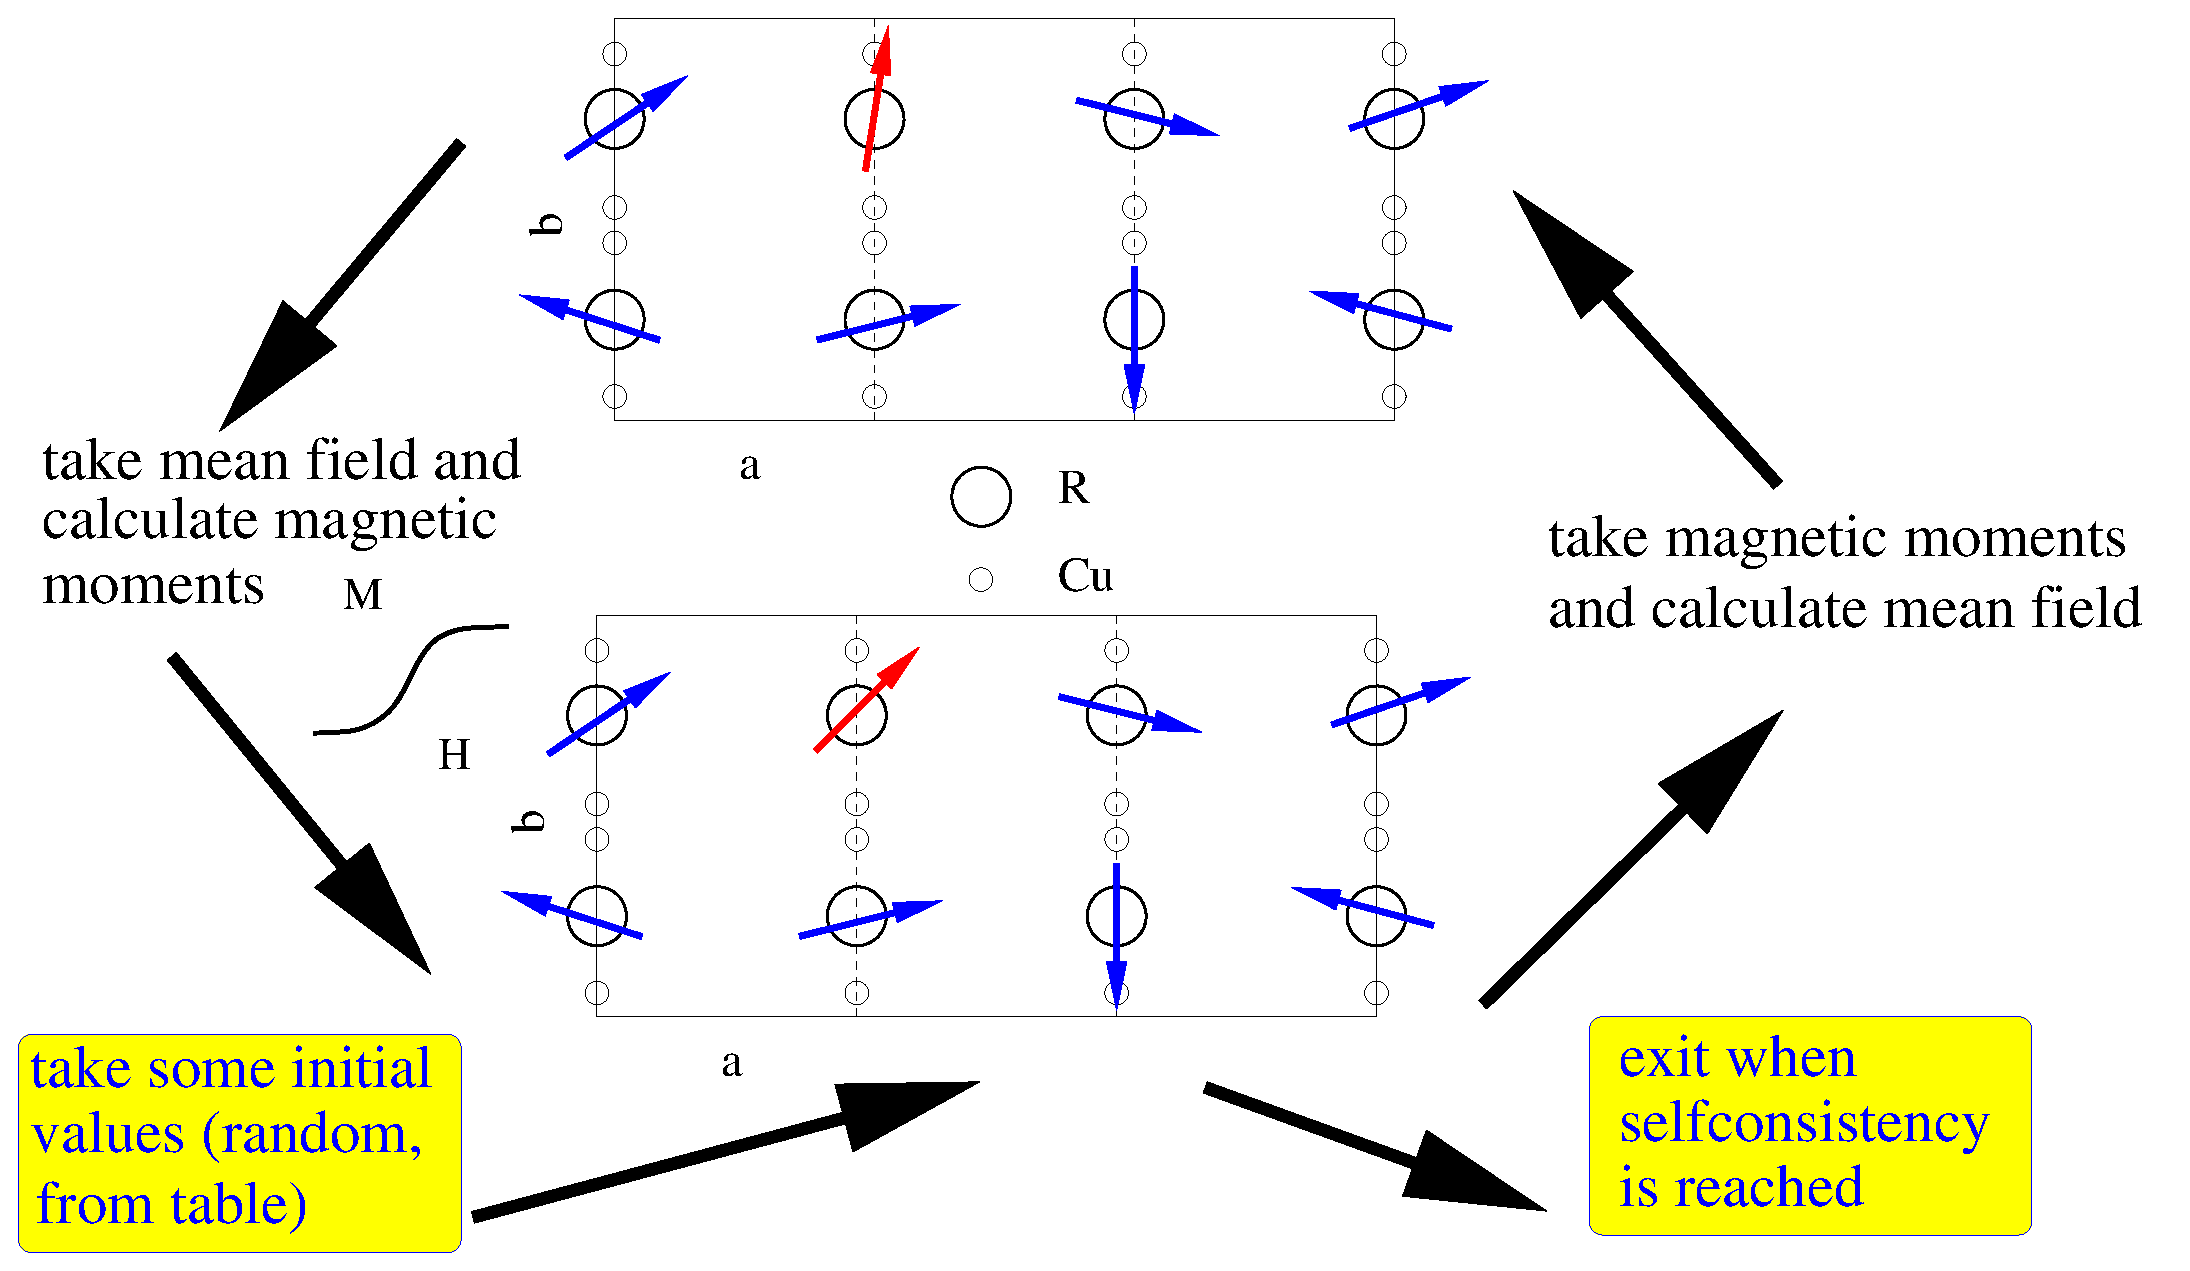
\includegraphics[angle=0,width=0.9\columnwidth]{figsrc/fecalc.eps}
\caption{\label{fecalc}Mean field process of sub {\prg fecalc}.}
\end{figure}

 
\subsubsection{Example {\prg mcphas.ini\index{mcphas.ini}} file for a simple antiferromagnet}

Here is an example of {\prg mcphas.ini\index{mcphas.ini}}, the comments describe the meaning of the different
parameters:

\section{{\prg mcphas} - calculation of thermodynamic properties (Magnetisation, Susceptibility, Specific Heat, Neutron %%@
Diffraction, etc.)}
\label{runmcphas}

In order to perform calculations beyond the capabilities of {\prg cfield\index{cfield}} it is necessary
to use the program {\prg mcphas}. 
\begin{itemize}
\item As a first step it is possible to
calculate the thermodynamic properties such as magnetisation or specific heat
considering only single ion effects. In this case all the exchange parameters
have to be set to zero in {\prg mcphas.j\index{mcphas.j}}. 
\item for more advanced calculations the two - ion interactions have to be
considered and may lead to magnetic order. {\prg mcphas} can perform 
calculations in the ordered state in the following way: for 
a given temperature $T$ and magnetic field $\mbf H$ (vector)
several possible magnetic structures are stabilised
by a mean field algorithm and the free energy is 
calculated. The initial values for this mean-field procedure are
modified by a Monte Carlo process.


The temperature and magnetic field is varied during the calculation
and thereby it is possible to map out the magnetic phase diagram.
\end{itemize}

The program produces a plot of the stabilised magnetic
structures and the magnetisation on screen, the
output files contain additional information 
such as calculated magnetoelastic and  neutron-scattering
data. Several graphic programs easy the visualisation of the
calculated data (section~\ref{graphics}).



\subsection{Input Files}
The program {\prg McPhase} needs the following input files (all in the same directory)
 in order to run:

\begin{enumerate}
\item {\prg mcphas.ini\index{mcphas.ini}}
 - controlling the algorithm
\item {\prg mcphas.j\index{mcphas.j}}
  - lattice and exchange parameters
\item {\prg mcphas.tst\index{mcphas.tst}(optional)}  - test spin configurations
\item {\prg single-ion property files}
\item {\prg directory ./results/}
 - directory where calculated data is stored
\item {\prg directory ./fit} - experimental data for fit (optional)
\end{enumerate}


 All
 of these input files have to be in one directory and the program
has to be started in this directory. The results of the simulation
are then stored in the  subdirectory ./results/, which must exist before starting
the program 
... see directory ./examples/ for some examples.
 In order to prepare these files
for a new calculation it is best to take them from an example, copy the files
to a new directory and make the
modifications  to adapt them to the new problem.

\subsubsection{Example - a simple antiferromagnet}

In the following description of the input files we will always refer
to a simple example: a simple antiferromagnet
on a primitive orthorhombic lattice. The first time user
will thus have a simple example to follow, all corresponding
files are given in the directory {\prg tutorial/03magnetic\_phases\_mcphas/simpleAF}.
 

\subsubsection{{\prg mcphas.ini\index{mcphas.ini}} - controlling the algorithm}
   Initial file containing algorithm control parameters, for instance the range and spacing of
   propagation vectors Q or the number of Monte Carlo trials for initial spin configurations
    - {\em mind}: this
   file is rewritten and reread  when running the program and may be changed by the
   user in order to manipulate the running simulation.

{\prg mcphas.ini\index{mcphas.ini}} consists of several sections:
\begin{description}
\item [MCPHASE RUNTIME CONTROL:] this section contains the parameters
controlling the status of the calculation.
\item [XY PHASEDIAGRAM PARAMETERS:] here the temperature and field range and
step widths of the calculation are specified.
The definition of the x and y
axis in terms of temperature and magnetic field is followed by the
corresponding range and step width. An offset may be given for all
field and temperature values.
Note that for most cases of interest
this offset is zero (T0=0, Ha0=0, Hb0=0, Hc0=0).
 For the simple case of calculating a Temperature-Field phase diagram
 It is just necessary to set xT=1 and give the temperature range by
xmin/xmax/xstep. For field in b direction then just set yHb=1 and 
define the range in ymin/ymax/ystep.
In case of non-orthogonal axes the applied magnetic field
components $Ha, Hb, Hc$ refer to the orthogonal coordinate system
defined with respect to the nonorthogonal lattice $\mbf a,\mbf b,\mbf c$ as
$Hb||\mbf b$, $Hc||(\mbf a \times \mbf b)$ and $Ha$ perpendicular to $Hb$ and $Hc$.

\item [GENERATION OF SPINCONFIGURATIONS:] at the beginning of the program
some initial values of spin configurations are generated from a set of 
propagation vectors. This section defines the range of propagation vectors
and the step width.
Depending on the value of the propagation Q with respect to the primitive reciprocal lattice
1-, 2- or 3-dimensional simulations of magnetic lattices
are possible. It is advisable to 
think carefully about the chosen range and spacing of Q vectors in order
to limit calculation time.
 
For example a good starting point is to begin with a calculation with large
step widths (e.g. 0.1)  covering the Brillouin zone. This should give an idea
of the propagation vectors which are stabilised. An advanced calculation
could then fine tune the propagation and determine its accurate value (using
small step widths in a limited area of the zone).
The verbose option of {\prg mcphas} allows to inspect the propagation vectors
which are actually used in the calculation.
Trick: in order to get a quick overview of the
q-vector range covered by the mcphas\index{mcphas} simulation start mcphas, exit and 
just type {\prg felog ./results/mcphas.qvc} (need {\prg perl,perldl,pdl,pgplot} packages).

In order to limit calculation time, the maximum periodicity
of the magnetic unit cell with respect to the crystallographic unit cell 
(maxqperiod) and the maximum number of spins in the magnetic unit cell 
(maxnofspins) can be limited. Also the maximum number of test spin configurations
in the internal table can be limited (maxnoftestspincf).
A critical feature with respect to calculation time is also the number of
spin configurations which are generated by a random process from a tabulated
SPINCONFIGURATIONS during the calculation. 

In summary the variables in this section are mainly important to adapt the
program to a given computer system with finite speed. They have to be set
to optimise between speed and accuracy of the calculation. In order to
find appropriate values it is best to perform some calculations 
and restrict the parameters step by step if insufficient speed is obtained.
Also the examples included in the program package may serve as starting
points.

\item [PARAMETERS FOR SUB FECALC SELFCONSISTENCY PROCESS:] the most important
procedure in the module {\prg mcphas} is the sub fecalc. In this part of the 
program the self consistent calculation of the magnetic moment configuration
is performed as shown schematically in fig.~\ref{fecalc}. 
In the mean field approximation the Hamiltonian~(\ref{hamilton}) is approximated
by

\begin{equation}
 {\mathcal H}=\sum_n H_{SI}^n + E_{corr}
\end{equation}

with the single ion Hamiltonian (in case of module {\prg so1ion\index{so1ion}})

\begin{equation}
H_{SI}^n=  B_l^m O_{lm}({\mbf J}^n) 
	     - g_{Jn} \mu_B {\mbf J}^n {\mbf H^n_{eff}} 
\end{equation}

and the correction term

\begin{equation}
E_{corr}=\frac{1}{2}\sum_{n} g_{Jn} \mu_B \langle {\mbf J}^n
 \rangle (\mbf H^n_{eff}-\mbf H) 
\end{equation}

and with the mean fields $ \mbf H^n_{eff}$ given by

\begin{equation}\label{meanfield}
\mbf H^n_{eff}=\mbf H + \mbf H^n_{xc}=\mbf H+\sum_{{\mbf G'}n'} \frac{{\mathcal J}
(\mbf r_n-(\mbf G'+\mbf r_{n'}))}{g_{Jn}\mu_B } \langle{\mbf
J}^{n'}\rangle
\end{equation}

These mean fields and the moments $\langle \mbf J^n \rangle$ 
are determined in a self consistent
way. For a given magnetic unit cell and initial configuration 
of magnetic moments
the mean fields are calculated according to equation~(\ref{meanfield}). 
Then, for each
magnetic ion the single ion property module is taken 
and the magnetic moment $\langle \mbf J^n \rangle$ is 
calculated from it's mean field. The mean fields are used again in equation~(\ref{meanfield})
and so on .... until convergence is reached. 
Then, the free energy ($f=-kT\sum_n \ln(z_n) + E_{corr}$ ) 
of the stabilised
configuration is calculated (this is why this sub is called {\prg fecalc}). 
The free energies of a lot of different stabilised configurations have to
be compared in order to find out which configuration has lowest free energy, i.e.
is stable in thermal  equilibrium.

It may happen that this process does
not converge due to bad choice of the initial configuration, therefore a maximum number
of mean field loops has to be given by the user.
The results of a calculation may be significantly influenced by
changing parameters such as the maximum number of iteration loops 
in this section. 
In fact the simulation is always a compromise of calculation time and accuracy: if only
a few initial spin configurations are tried at each (H-T) point, the calculation speed is
fast, however it is possible that the program misses the magnetic structure with the
lowest free energy. The same holds if other critical parameters of the simulation are
restricted too much.
 

\item [OUTPUT OF PHYSICAL PROPERTIES:]
Some options for the output of the calculation can be changed in this section.
\end{description}

\begin{figure}[hb]
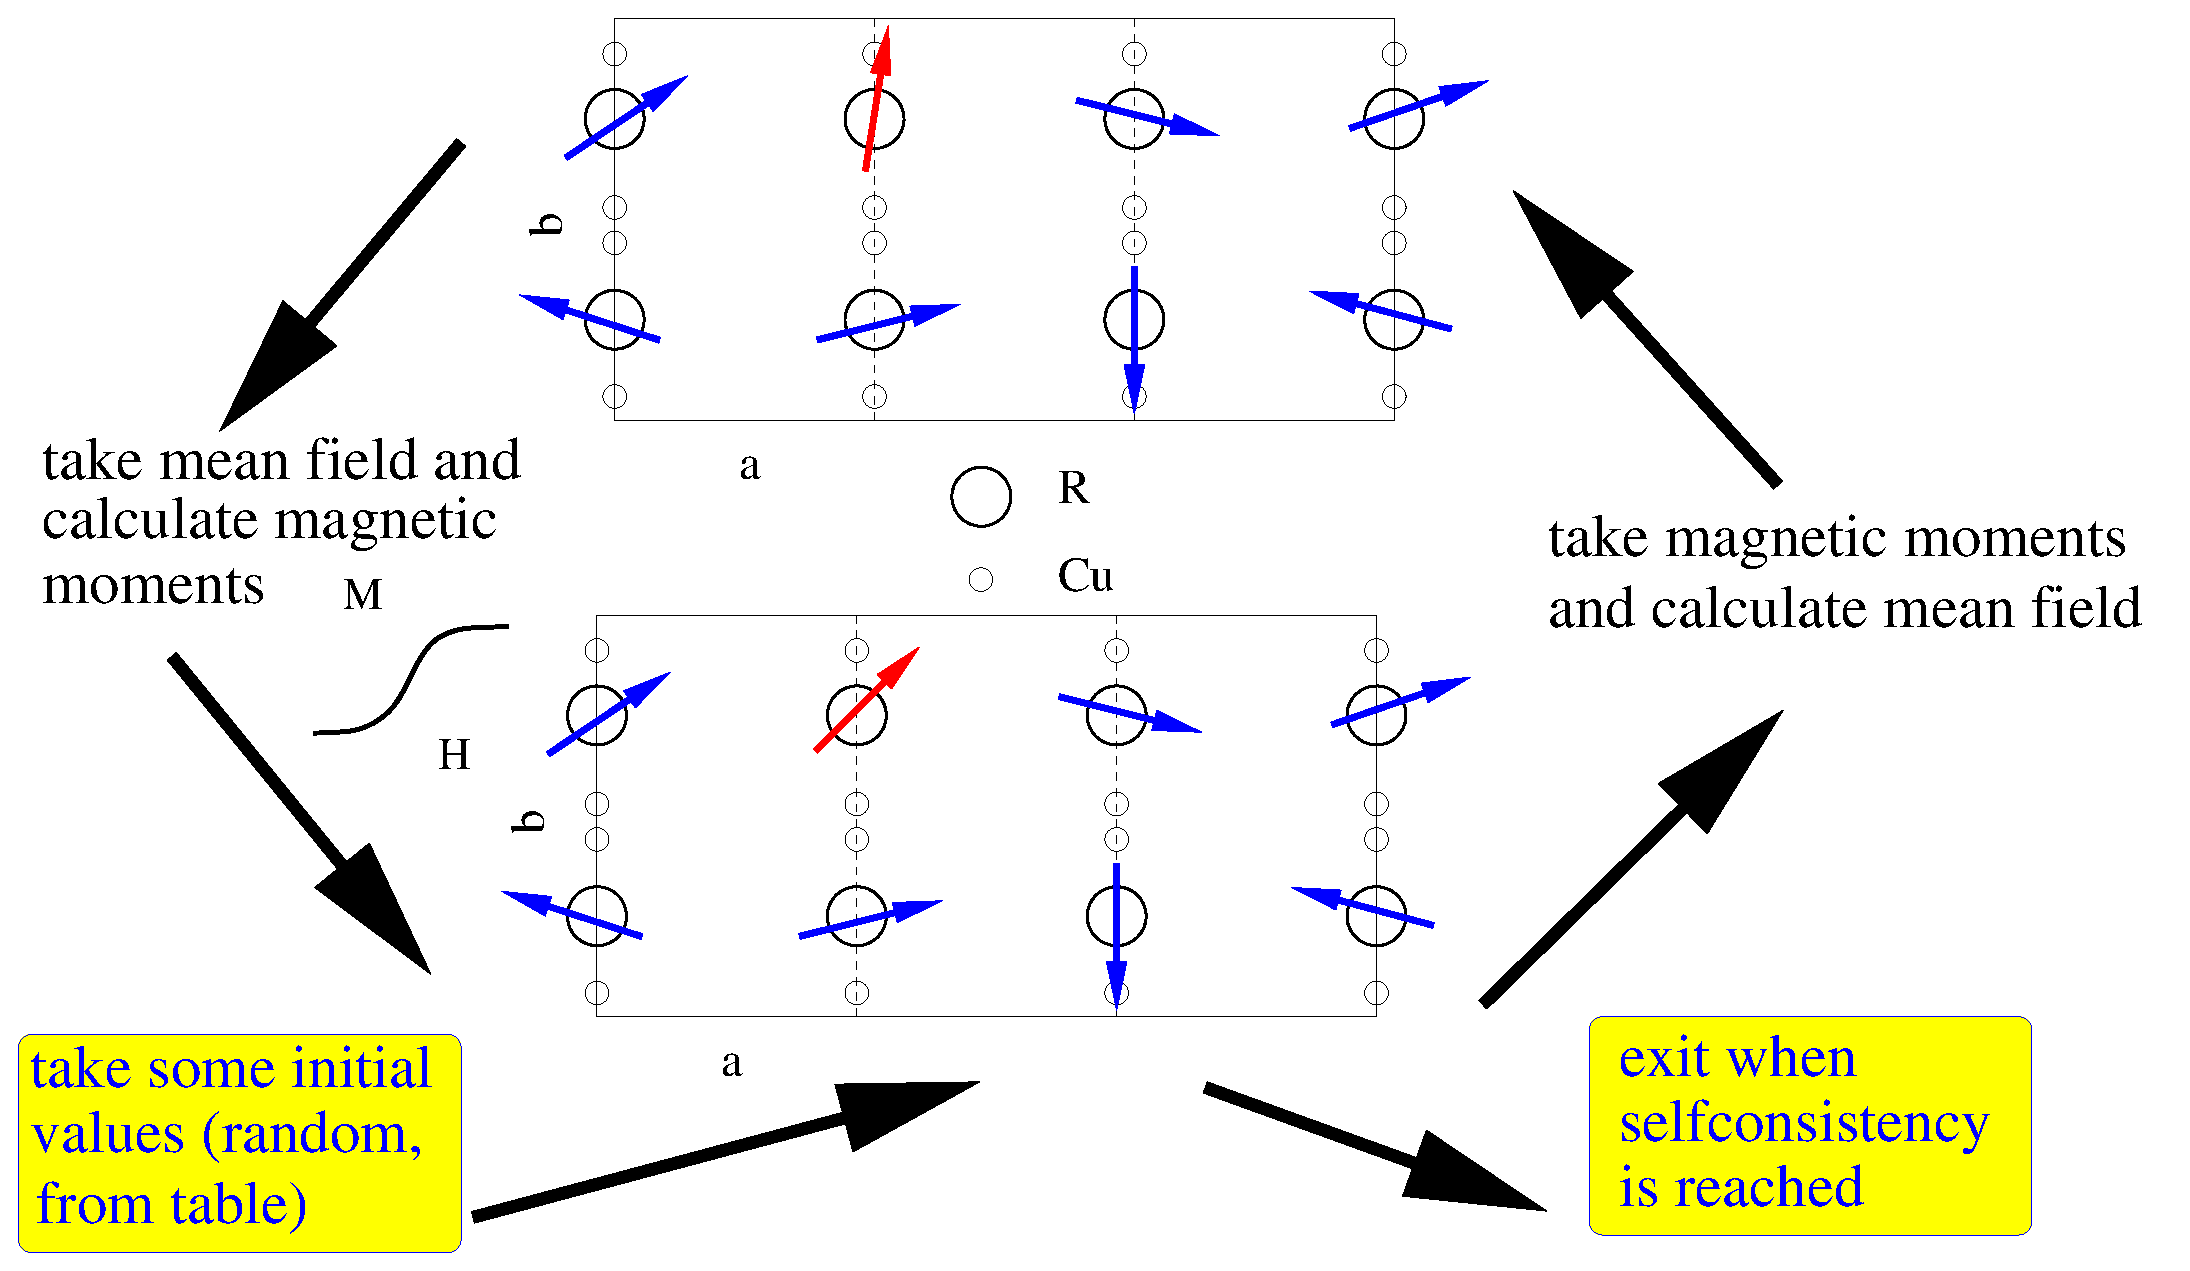
\includegraphics[angle=0,width=0.9\columnwidth]{figsrc/fecalc.eps}
\caption{\label{fecalc}Mean field process of sub {\prg fecalc}.}
\end{figure}

 
\subsubsection{Example {\prg mcphas.ini\index{mcphas.ini}} file for a simple antiferromagnet}

Here is an example of {\prg mcphas.ini\index{mcphas.ini}}, the comments describe the meaning of the different
parameters:

\section{{\prg mcphas} - calculation of thermodynamic properties (Magnetisation, Susceptibility, Specific Heat, Neutron %%@
Diffraction, etc.)}
\label{runmcphas}

In order to perform calculations beyond the capabilities of {\prg cfield\index{cfield}} it is necessary
to use the program {\prg mcphas}. 
\begin{itemize}
\item As a first step it is possible to
calculate the thermodynamic properties such as magnetisation or specific heat
considering only single ion effects. In this case all the exchange parameters
have to be set to zero in {\prg mcphas.j\index{mcphas.j}}. 
\item for more advanced calculations the two - ion interactions have to be
considered and may lead to magnetic order. {\prg mcphas} can perform 
calculations in the ordered state in the following way: for 
a given temperature $T$ and magnetic field $\mbf H$ (vector)
several possible magnetic structures are stabilised
by a mean field algorithm and the free energy is 
calculated. The initial values for this mean-field procedure are
modified by a Monte Carlo process.


The temperature and magnetic field is varied during the calculation
and thereby it is possible to map out the magnetic phase diagram.
\end{itemize}

The program produces a plot of the stabilised magnetic
structures and the magnetisation on screen, the
output files contain additional information 
such as calculated magnetoelastic and  neutron-scattering
data. Several graphic programs easy the visualisation of the
calculated data (section~\ref{graphics}).



\subsection{Input Files}
The program {\prg McPhase} needs the following input files (all in the same directory)
 in order to run:

\begin{enumerate}
\item {\prg mcphas.ini\index{mcphas.ini}}
 - controlling the algorithm
\item {\prg mcphas.j\index{mcphas.j}}
  - lattice and exchange parameters
\item {\prg mcphas.tst\index{mcphas.tst}(optional)}  - test spin configurations
\item {\prg single-ion property files}
\item {\prg directory ./results/}
 - directory where calculated data is stored
\item {\prg directory ./fit} - experimental data for fit (optional)
\end{enumerate}


 All
 of these input files have to be in one directory and the program
has to be started in this directory. The results of the simulation
are then stored in the  subdirectory ./results/, which must exist before starting
the program 
... see directory ./examples/ for some examples.
 In order to prepare these files
for a new calculation it is best to take them from an example, copy the files
to a new directory and make the
modifications  to adapt them to the new problem.

\subsubsection{Example - a simple antiferromagnet}

In the following description of the input files we will always refer
to a simple example: a simple antiferromagnet
on a primitive orthorhombic lattice. The first time user
will thus have a simple example to follow, all corresponding
files are given in the directory {\prg tutorial/03magnetic\_phases\_mcphas/simpleAF}.
 

\subsubsection{{\prg mcphas.ini\index{mcphas.ini}} - controlling the algorithm}
   Initial file containing algorithm control parameters, for instance the range and spacing of
   propagation vectors Q or the number of Monte Carlo trials for initial spin configurations
    - {\em mind}: this
   file is rewritten and reread  when running the program and may be changed by the
   user in order to manipulate the running simulation.

{\prg mcphas.ini\index{mcphas.ini}} consists of several sections:
\begin{description}
\item [MCPHASE RUNTIME CONTROL:] this section contains the parameters
controlling the status of the calculation.
\item [XY PHASEDIAGRAM PARAMETERS:] here the temperature and field range and
step widths of the calculation are specified.
The definition of the x and y
axis in terms of temperature and magnetic field is followed by the
corresponding range and step width. An offset may be given for all
field and temperature values.
Note that for most cases of interest
this offset is zero (T0=0, Ha0=0, Hb0=0, Hc0=0).
 For the simple case of calculating a Temperature-Field phase diagram
 It is just necessary to set xT=1 and give the temperature range by
xmin/xmax/xstep. For field in b direction then just set yHb=1 and 
define the range in ymin/ymax/ystep.
In case of non-orthogonal axes the applied magnetic field
components $Ha, Hb, Hc$ refer to the orthogonal coordinate system
defined with respect to the nonorthogonal lattice $\mbf a,\mbf b,\mbf c$ as
$Hb||\mbf b$, $Hc||(\mbf a \times \mbf b)$ and $Ha$ perpendicular to $Hb$ and $Hc$.

\item [GENERATION OF SPINCONFIGURATIONS:] at the beginning of the program
some initial values of spin configurations are generated from a set of 
propagation vectors. This section defines the range of propagation vectors
and the step width.
Depending on the value of the propagation Q with respect to the primitive reciprocal lattice
1-, 2- or 3-dimensional simulations of magnetic lattices
are possible. It is advisable to 
think carefully about the chosen range and spacing of Q vectors in order
to limit calculation time.
 
For example a good starting point is to begin with a calculation with large
step widths (e.g. 0.1)  covering the Brillouin zone. This should give an idea
of the propagation vectors which are stabilised. An advanced calculation
could then fine tune the propagation and determine its accurate value (using
small step widths in a limited area of the zone).
The verbose option of {\prg mcphas} allows to inspect the propagation vectors
which are actually used in the calculation.
Trick: in order to get a quick overview of the
q-vector range covered by the mcphas\index{mcphas} simulation start mcphas, exit and 
just type {\prg felog ./results/mcphas.qvc} (need {\prg perl,perldl,pdl,pgplot} packages).

In order to limit calculation time, the maximum periodicity
of the magnetic unit cell with respect to the crystallographic unit cell 
(maxqperiod) and the maximum number of spins in the magnetic unit cell 
(maxnofspins) can be limited. Also the maximum number of test spin configurations
in the internal table can be limited (maxnoftestspincf).
A critical feature with respect to calculation time is also the number of
spin configurations which are generated by a random process from a tabulated
SPINCONFIGURATIONS during the calculation. 

In summary the variables in this section are mainly important to adapt the
program to a given computer system with finite speed. They have to be set
to optimise between speed and accuracy of the calculation. In order to
find appropriate values it is best to perform some calculations 
and restrict the parameters step by step if insufficient speed is obtained.
Also the examples included in the program package may serve as starting
points.

\item [PARAMETERS FOR SUB FECALC SELFCONSISTENCY PROCESS:] the most important
procedure in the module {\prg mcphas} is the sub fecalc. In this part of the 
program the self consistent calculation of the magnetic moment configuration
is performed as shown schematically in fig.~\ref{fecalc}. 
In the mean field approximation the Hamiltonian~(\ref{hamilton}) is approximated
by

\begin{equation}
 {\mathcal H}=\sum_n H_{SI}^n + E_{corr}
\end{equation}

with the single ion Hamiltonian (in case of module {\prg so1ion\index{so1ion}})

\begin{equation}
H_{SI}^n=  B_l^m O_{lm}({\mbf J}^n) 
	     - g_{Jn} \mu_B {\mbf J}^n {\mbf H^n_{eff}} 
\end{equation}

and the correction term

\begin{equation}
E_{corr}=\frac{1}{2}\sum_{n} g_{Jn} \mu_B \langle {\mbf J}^n
 \rangle (\mbf H^n_{eff}-\mbf H) 
\end{equation}

and with the mean fields $ \mbf H^n_{eff}$ given by

\begin{equation}\label{meanfield}
\mbf H^n_{eff}=\mbf H + \mbf H^n_{xc}=\mbf H+\sum_{{\mbf G'}n'} \frac{{\mathcal J}
(\mbf r_n-(\mbf G'+\mbf r_{n'}))}{g_{Jn}\mu_B } \langle{\mbf
J}^{n'}\rangle
\end{equation}

These mean fields and the moments $\langle \mbf J^n \rangle$ 
are determined in a self consistent
way. For a given magnetic unit cell and initial configuration 
of magnetic moments
the mean fields are calculated according to equation~(\ref{meanfield}). 
Then, for each
magnetic ion the single ion property module is taken 
and the magnetic moment $\langle \mbf J^n \rangle$ is 
calculated from it's mean field. The mean fields are used again in equation~(\ref{meanfield})
and so on .... until convergence is reached. 
Then, the free energy ($f=-kT\sum_n \ln(z_n) + E_{corr}$ ) 
of the stabilised
configuration is calculated (this is why this sub is called {\prg fecalc}). 
The free energies of a lot of different stabilised configurations have to
be compared in order to find out which configuration has lowest free energy, i.e.
is stable in thermal  equilibrium.

It may happen that this process does
not converge due to bad choice of the initial configuration, therefore a maximum number
of mean field loops has to be given by the user.
The results of a calculation may be significantly influenced by
changing parameters such as the maximum number of iteration loops 
in this section. 
In fact the simulation is always a compromise of calculation time and accuracy: if only
a few initial spin configurations are tried at each (H-T) point, the calculation speed is
fast, however it is possible that the program misses the magnetic structure with the
lowest free energy. The same holds if other critical parameters of the simulation are
restricted too much.
 

\item [OUTPUT OF PHYSICAL PROPERTIES:]
Some options for the output of the calculation can be changed in this section.
\end{description}

\begin{figure}[hb]
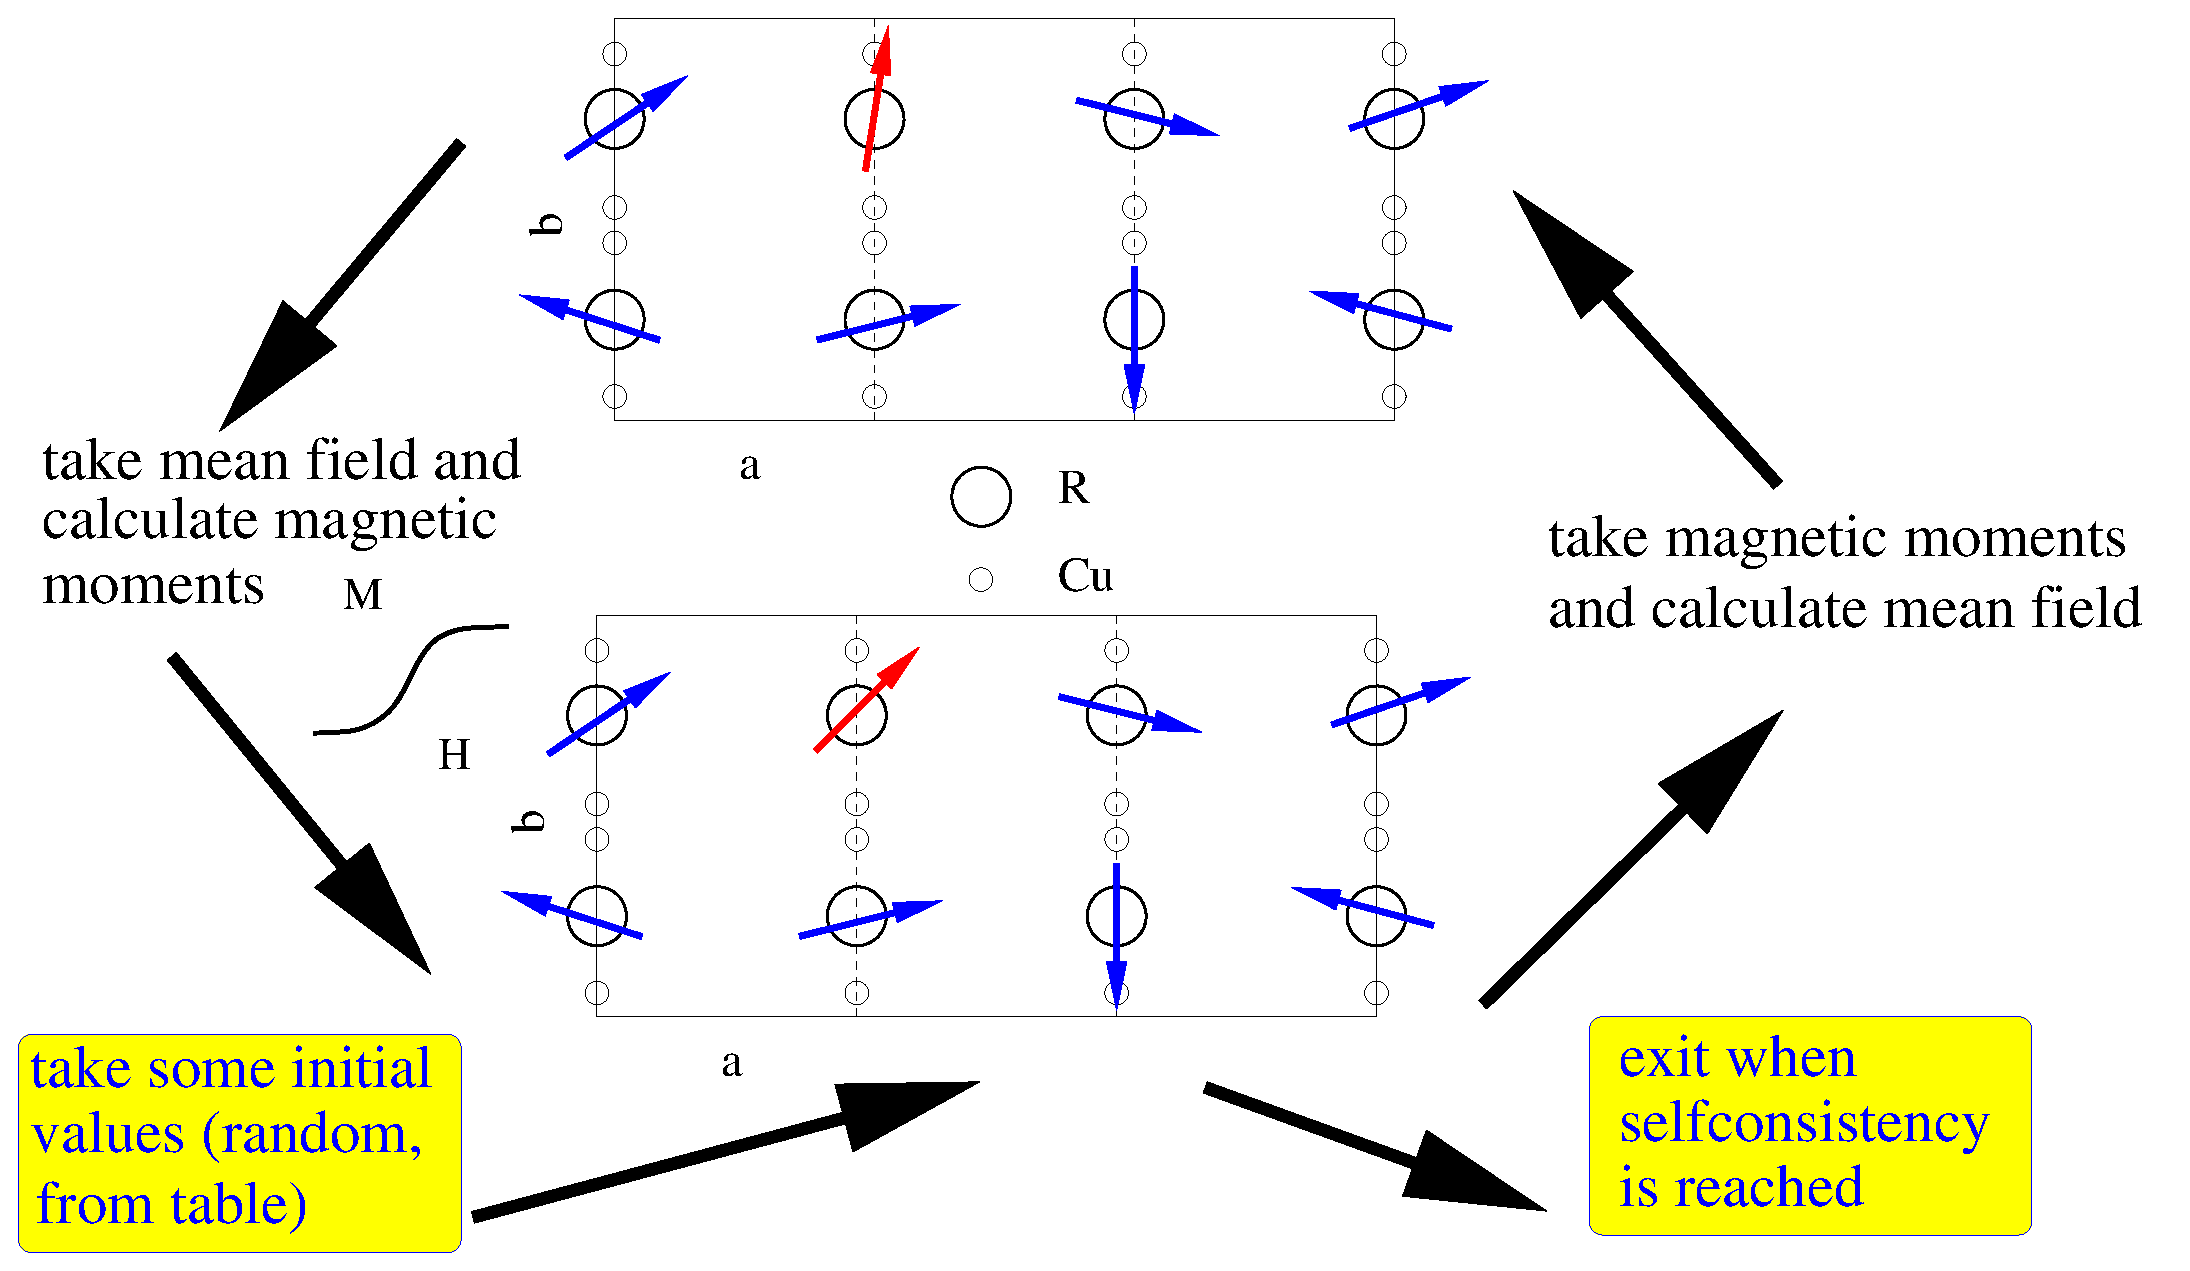
\includegraphics[angle=0,width=0.9\columnwidth]{figsrc/fecalc.eps}
\caption{\label{fecalc}Mean field process of sub {\prg fecalc}.}
\end{figure}

 
\subsubsection{Example {\prg mcphas.ini\index{mcphas.ini}} file for a simple antiferromagnet}

Here is an example of {\prg mcphas.ini\index{mcphas.ini}}, the comments describe the meaning of the different
parameters:

\input{mcphas.ini}



\subsubsection{{\prg mcphas.j\index{mcphas.j}} - lattice and exchange parameters}\label{mcphasj}
This file provides the information about 
the crystallographic
 structure and the magnetic exchange interactions.
For every atom in the crystallographic basis there
has to be given the coordinates, the number of neighbours to be considered, the 
Land\'e factor $g_J$, the single ion property filename and  a set of exchange parameters.
If the exchange parameters (and neighbour positions) are not known for your system, you 
can use the program module {\prg makenn\index{makenn}} (see section \ref{addprog}) to generate 
a list of nearest neighbours and
exchange parameters, currently implemented in {\prg makenn\index{makenn}} are dipolar interactions,
exchange interactions via the Bethe-Slater curve or the RKKY model. Note that in order
to use {\prg makenn\index{makenn}} you have to set up a working {\prg mcphas.j\index{mcphas.j}} file, which may or
may not contain neighbours and interactions.

Use program {\prg addj\index{addj}} to add exchange parameter set stored in different 
such {\prg .j} files (see section~\ref{addprog}).



\begin{description}
\item [Line 1,2:] Comment Lines
\item [Line 3:] lattice constants a,b,c and crystal angles alpha, beta, gamma 
\item [Line 4-6:] primitive lattice vectors
\item [Line 7:] Number of atoms in the primitive crystallographic unit cell ({\prg nofatoms})
\item [Line 8:] a comment line with stars
\item [Line 9:] coordinates  ($d_a$,$d_b$,$d_c$) of 1$^{st}$ magnetic ion in the crystallographic unit cell  with
respect to the lattice vectors $\vec a$,$\vec b$,$\vec c$. The number of neighbours of this 
ion, for which interaction constants are given in the interaction table (nofneighbours). 
If {\prg diagonalexchange}
is set to 0 the 9 components of the exchange tensor are given in column 4-12. 
If {\prg diagonalexchange}
 is 1, only 3 components are given (column 4-6).
If {\prg diagonalexchange}
 is 2, specific components of the exchange tensor can be given in columns 4 onwards. The indices of these components
 must be given in the following line (Line 9a below).
The Land\'e factor of the ion (gJ) and the file name of the corresponding single ion
parameter file (cffilename).
\item [Line 9a:]  If {\prg diagonalexchange=2}, then this line gives the indices of the exchange tensor corresponding to 
 the columns 4 onwards. It must have a variable called {\prg indexexchange} followed by a list of names of components of the interaction
 tensor separated by space. E.g.
 \verb|  #! indexexchange= JaJb JbJc  | 
means column 4 gives the the interaction constant between the
 first angular momentum component of the current ion with the second angular momentum component of its neighbour, whilst 
 column 5 has the interaction constant between the second angular momentum component of this ion with the third component of its
 neighbour. Alternatively, pairs of numbers may be given, as in \verb|  #! indexexchange= 1,2 2,3  |
 Additionally another parameter {\prg symmetricexchange} can be set to 1, where the value in each column is also used 
 for the transposed tensor component. Thus \verb|  #! symmetricexchange=1 indexexchange= JaJb  | is the same as \\
 \verb|  #! indexexchange= JaJb JbJa  | where the 4th and 5th column are the same.
\item [Line 10:]  Comment line
\item [Line 11-(10+nofneighbours):] Interaction table for ion number 1.   
Note: the neighbour coordinates (column 1-3) are given with respect to the lattice vectors
$\vec a$,$\vec b$,$\vec c$. The program then calculates from these values the coordinates
with respect to the primitive lattice $\vec r_1$,~$\vec r_2$,~$\vec r_3$.
($ d_a \vec a + d_b \vec b + d_c \vec c = d_1 \vec r_1 + d_2 \vec r_2 + d_3 \vec r_3$).
Column 4,5,6 \dots contain the components of the interaction tensor $\stackrel{=}{\mathcal J}$. 
Note that in case of non-orthogonal axes the 
components of the moments and the interaction tensor $Ja, Jb, Jc, Jaa, Jbb, Jcc, Jab ...$ 
refer to the orthogonal coordinate system
defined with respect to the nonorthogonal lattice $\vec a,\vec b,\vec c$ as
$Jb||\vec b$, $Jc||(\vec a \times \vec b)$ and $Ja$ perpendicular to $Jb$ and $Jc$.
\item [Line (11+nofneighbours) - end:] for each ion in the unit cell line 8 - (10+nofneighbours)
are repeated.
\end{description}


\vspace{0.5cm}

{\small {\bf Information for experienced users:}
\begin{description}
\item[\prg mcphas.jjj:]
format of exchange parameter file, which only needs a reduced set of exchange
parameters in the input file. Using the program {\prg jjj2j} the file can be transformed
to {\prg mcphas.j\index{mcphas.j}} by adding lines for all the equivalent neighbours. The format definition
of {\prg mcphas.jjj} is the same as {\prg mcphas.j\index{mcphas.j}}, however each line denotes several
equivalent neighbour atoms (instead of only one in {\prg mcphas.j\index{mcphas.j}}) according to the
 following rules:
\begin{itemize}
\item If a nonzero coordinate $d_a$ (or $d_b$,$d_c$) in the interaction table
 corresponds to it's value at the nearest
 lattice point of the primitive lattice,
  additional interactions of the same size
with  neighbours with coordinate $-d_a$ (or $-d_b$,$-d_c$, respectively)
are taken into account. This
holds for each of the three coordinates $d_a$,$d_b$ and $d_c$
 resulting in a maximum
number of 8 equivalent neighbours per line in the interaction table.
\item If the value of $d_a$ (or $d_b$,$d_c$) is zero or differs
from it's value at the nearest lattice point of the primitive lattice, it is 
changed to the value at the nearest lattice point and {\bf no} interaction 
with  neighbours with coordinates $-d_a$ (or $-d_b$,$-d_c$) is
 taken into account. If such
 interaction is needed it may be given in a different line and may
have different magnitude. In this way also crystallographic lattices
with no mirror symmetry may be described.
\end{itemize}
\item[\prg mcphas.coq:]   exchange parameters etc [ in old format]...see examples for details, use {\prg coq2jjj} to 
transform {\prg mcphas.coq} to {\prg mcphas.jjj} format
\end{description}

}


\subsubsection{Example {\prg mcphas.j\index{mcphas.j}} file for a simple antiferromagnet}

Here are example files of a tetragonal antiferromagnet with nearest neighbour interactions, all
files are equivalent:

{\small
\begin{verbatim} 
# simple antiferromagnet 
#<!--mcphase.mcphas.j-->
#***************************************************************
# Lattice Constants (A)
#! a=4.3843 b=4.3843 c=2.4194 alpha=  90 beta=  90 gamma=  90
#! r1a=   1 r2a=   0 r3a=   0
#! r1b=   0 r2b=   1 r3b=   0   primitive lattice vectors [a][b][c]
#! r1c=   0 r2c=   0 r3c=   1
#! nofatoms=1  nofcomponents=3  number of atoms in primitive unit cell/number of components of each spin
# ****************************************************************************
#! da=  0 [a] db=  0 [b] dc=  0 nofneighbours=2 diagonalexchange=0 gJ=0.857143 cffilename=Ce3p.sipf
# da[a] db[b] dc[c] Jaa[meV] Jbb[meV] Jcc[meV] Jab[meV] Jba[meV] Jac[meV] Jca[meV] Jbc[meV] Jcb[meV]
+0	+0	+1	-0.1	-0.1	-0.1   0  0  0  0  0  0
+0	+0	-1	-0.1	-0.1	-0.1   0  0  0  0  0  0
#\end{verbatim}
}

Using diagonalexchange this may be shortened to

{\small
\begin{verbatim} 
# simple antiferromagnet 
#<!--mcphase.mcphas.j-->
#***************************************************************
# Lattice Constants (A)
#! a=4.3843 b=4.3843 c=2.4194 alpha=  90 beta=  90 gamma=  90
#! r1a=   1 r2a=   0 r3a=   0
#! r1b=   0 r2b=   1 r3b=   0   primitive lattice vectors [a][b][c]
#! r1c=   0 r2c=   0 r3c=   1
#! nofatoms=1  nofcomponents=3  number of atoms in primitive unit cell/number of components of each spin
# ****************************************************************************
#! da=  0 [a] db=  0 [b] dc=  0 nofneighbours=2 diagonalexchange=1 gJ=0.857143 cffilename=Ce3p.sipf
# da[a] db[b] dc[c] Jaa[meV] Jbb[meV] Jcc[meV] Jab[meV] Jba[meV] Jac[meV] Jca[meV] Jbc[meV] Jcb[meV]
+0	+0	+1	-0.1	-0.1	-0.1   
+0	+0	-1	-0.1	-0.1	-0.1   
#\end{verbatim}
}

with indexexchange option the sequence of two ion interaction parameters can be changed and
zero parameters may be omitted:

{\small
\begin{verbatim} 
# simple antiferromagnet 
#<!--mcphase.mcphas.j-->
#***************************************************************
# Lattice Constants (A)
#! a=4.3843 b=4.3843 c=2.4194 alpha=  90 beta=  90 gamma=  90
#! r1a=   1 r2a=   0 r3a=   0
#! r1b=   0 r2b=   1 r3b=   0   primitive lattice vectors [a][b][c]
#! r1c=   0 r2c=   0 r3c=   1
#! nofatoms=1  nofcomponents=3  number of atoms in primitive unit cell/number of components of each spin
# ****************************************************************************
#! da=  0 [a] db=  0 [b] dc=  0 nofneighbours=2 diagonalexchange=2 gJ=0.857143 cffilename=Ce3p.sipf
# da[a] db[b] dc[c] Jaa[meV] Jbb[meV] Jcc[meV] Jab[meV] Jba[meV] Jac[meV] Jca[meV] Jbc[meV] Jcb[meV]
#! indexexchange = JaJa JaJc JcJa JbJb JcJc
+0	+0	+1	-0.1 0 0 -0.1	-0.1  
+0	+0	-1	-0.1 0 0 -0.1	-0.1  
#\end{verbatim}
}

{\small
\begin{verbatim} 
# simple antiferromagnet 
#<!--mcphase.mcphas.j-->
#***************************************************************
# Lattice Constants (A)
#! a=4.3843 b=4.3843 c=2.4194 alpha=  90 beta=  90 gamma=  90
#! r1a=   1 r2a=   0 r3a=   0
#! r1b=   0 r2b=   1 r3b=   0   primitive lattice vectors [a][b][c]
#! r1c=   0 r2c=   0 r3c=   1
#! nofatoms=1  nofcomponents=3  number of atoms in primitive unit cell/number of components of each spin
# ****************************************************************************
#! da=  0 [a] db=  0 [b] dc=  0 nofneighbours=2 diagonalexchange=2 gJ=0.857143 cffilename=Ce3p.sipf
# da[a] db[b] dc[c] Jaa[meV] Jbb[meV] Jcc[meV] Jab[meV] Jba[meV] Jac[meV] Jca[meV] Jbc[meV] Jcb[meV]
#! indexexchange = 1,1 1,3, 3,1 2,2 3,3
+0	+0	+1	-0.1 0 0 -0.1	-0.1  
+0	+0	-1	-0.1 0 0 -0.1	-0.1  
#\end{verbatim}
}


using symmetricexchange together with indexexchange will assume that the interaction tensor is symmetic and 
only half of it may be given:

{\small
\begin{verbatim} 
# simple antiferromagnet 
#<!--mcphase.mcphas.j-->
#***************************************************************
# Lattice Constants (A)
#! a=4.3843 b=4.3843 c=2.4194 alpha=  90 beta=  90 gamma=  90
#! r1a=   1 r2a=   0 r3a=   0
#! r1b=   0 r2b=   1 r3b=   0   primitive lattice vectors [a][b][c]
#! r1c=   0 r2c=   0 r3c=   1
#! nofatoms=1  nofcomponents=3  number of atoms in primitive unit cell/number of components of each spin
# ****************************************************************************
#! da=  0 [a] db=  0 [b] dc=  0 nofneighbours=2 diagonalexchange=2 gJ=0.857143 cffilename=Ce3p.sipf
# da[a] db[b] dc[c] Jaa[meV] Jbb[meV] Jcc[meV] Jab[meV] Jba[meV] Jac[meV] Jca[meV] Jbc[meV] Jcb[meV]
#! symmetricexchange=1 indexexchange = JaJa JaJc JbJb JcJc
+0	+0	+1	-0.1 0  -0.1	-0.1  
+0	+0	-1	-0.1 0  -0.1	-0.1  
#\end{verbatim}
}


\subsubsection{Single Ion Property Input Files}\label{sifile}

In order to speed up calculations or treat special problems a large 
variety of single ion modules is available. This includes the
option to load a user written single ion module. Details are 
given in chapter~\ref{simod}.

The first time user of {\prg McPhase} should use the module {\prg so1ion}\index{so1ion} and 
create an appropriate single ion property input file as described in
section \ref{cf1ion}. A good starting point are several examples
given in directory {\prg examples}.


\subsubsection{Example single ion property file  for a simple antiferromagnet}

Here is an example file {\prg mcphas.cf1} describing the anisotropy of a 
simple antiferromagnet with Ce atoms having basal plane anisotropy. Note the
axis convention xyz$||$abc, in case of non-orthogonal axes the convention 
is $y||\vec b$, $z||(\vec a \times \vec b)$ and $x$ perpendicular to $y$ and $z$.


\input{mcphas.cf1}

\subsubsection{{\prg mcphas.tst\index{mcphas.tst}} - input file of test spin-configurations (optional)}
This file is optional and contains
some test momentum configurations to be used for the calculation
             of the free energy. Mind that
\begin{itemize}
\item  in the file header the number of atoms in the primitive
       crystallographic unit cell and the number of components
       of the spin vector have to be given.
\item  at the end of the
 file there must be no empty lines !
\end{itemize}

The momentum - configurations tables always refer to spins sitting on
the primitive lattice ${\mbf r}_i$. If more than one atom is in
the primitive basis, the momentum gets $3n$ components ($n=$ number
of atoms in the crystallographic basis). See {\prg ./examples/ndcu2b\_new/} for
examples of a two atom basis. Units of these tables are that of total 
angular momentum $<J>$.

\subsubsection{Example {\prg mcphas.tst\index{mcphas.tst}} file  for a simple antiferromagnet}

Here is the file {\prg mcphas.tst\index{mcphas.tst}} for the simple antiferromagnet example
describing some spin configurations
to be used as starting values for the mean field process:

\input{mcphas.tst}
Note, in case of non-orthogonal axes the convention 
is $mb||\vec b$, $mc||(\vec a \times \vec b)$ and $ma$ perpendicular to $mb$ and $mc$.

\subsubsection{subdirectory {\prg ./results} - directory where calculated data is stored}

In order to be able to save the results of a calculation the directory {\prg ./results} has to
exist. Mind that all files in this directory will be overwritten without warning. 

\subsubsection{subdirectory {\prg ./fit} - experimental data for fit (optional) } 

In order that {\prg McPhase} can calculate the standard deviation between
 experimental data and the results of the simulation, some experimental data
 can be given in the subdirectory {\prg ./fit}. The filenames and the data-format
 are the same as the output files of {\prg McPhas}, e.g. {\prg mcphas.fum}, {\prg mcphas.hkl}
 etc. {\prg McPhase} looks into the directory {\prg ./fit} and if it finds any
 of these files, the standard deviation is increased correspondingly. 

What measurement data can be used to calculate a standard deviation ?

\begin{description}
\item[{\prg mcphas.fum}] if given in column 11, 12, 13 in {\prg ./fit/mcphas.fum} the
            magnetisation in the $a$, $b$ and $c$ direction is used for calculation
	    of the standard deviation sta. The standard deviation is calculated
	    as ${\rm sta}=\sum_{\rm data points i} ({\mbf m}_i^{calc}-{\mbf m}_i^{meas})^2$.
	    All three components of the magnetic moment have to be given and are used.

\end{description}

Note that the measured data has to be given in those (H-T) points which are 
calculated by mcphas\index{mcphas} in order to be used by the program to increase {\prg sta}.
It is usually most effective to fit only few data points, because a large set
of data points will not improve the quality of the fit and only require a large
amount of calculation time.



\subsection{Starting a simulation}
\label{start}

To start the simulation goto the directory containing the
input files {\prg mcphas.ini, mcphas.j, etc. } and type

\begin{description}
\item[\prg mcphas] to run the program generating stepwise $H-T$ values 
              in a loop given by {\prg mcphas.ini\index{mcphas.ini}} (you can also press the
              symbol in the {\prg McPhase - Explorer} window).
\item[\prg mcphas\index{mcphas} [file]]  to run the program with an input file --   
             {\prg file} contains T ha hb hc values to be calculated 
             if [file] is not given, xmin xmax xstep (xT xHa xHb xHc)
             ymin ymax ystep (yT yHa yHb yHc) is read from file {\prg mcphas.ini\index{mcphas.ini}}
	     and phase diagram is calculated
\item[\prg mcphas\index{mcphas} -h]  to  print help and version of {\prg McPhas}.
\item[\prg mcphas\index{mcphas} -stamax 14]  end mcphas\index{mcphas} if standard deviation exceeds 14.
\item[\prg mcphas\index{mcphas} -a] avoid overwriting output files in results, append new results to existing files
\item[\prg mcphas\index{mcphas} -v]  to  enable verbose mode with lots of messages of {\prg McPhas}. Specifically
the verbose mode enables the following features:
  \begin{itemize}
			          \item more information is printed out, 
			          \item the q-vectors file {\prg ./results/mcphas.qvc} will contain 
				    the explicit spin configurations
			          \item the display\index{display} on screen (ghostview window using 
				     {\prg ./results/.sps.eps}) will be updated not only 
				    when a H-T point has been finished but always 
				    when a structure with smaller free energy 
				    has been stabilised
  \end{itemize}
\item[\prg mcphasit\index{mcphas}] to start mcphase in commandline mode without opening any window
\end{description}

\vspace{1cm}
{\em Exercises:}
\begin{itemize}
\item Look at the input files for {\prg McPhase} given in the directory
{\prg examples/ndcu2b\_new}.  How many atoms are contained in the crystallographic basis ?
\item
Start the simulation by typing the command {\prg mcphas}.
\end{itemize}



\subsection{Options for a running simulation}
... when the program is running, the options in the main window
can be changed. Pressing ''displayall'' displays the current spin-configuration
at each iteration step. Pressing ''log fe vs Q'' appends free energy vs Q
data to {\prg mcphas.log} for every ($T-H$) point.


The file {\prg ./results/.spins.eps} is used to show the information about the currently calculated
spin structure on the screen using the postscript file viewer ghostview.

The file {\prg ./results/.mcphas.fum} contains the information of the magnetisation curve
which is currently calculated. This information is automatically displayed on the screen.


The program {\prg display} (see section \ref{display}) can be used 
for the online display\index{display} of any other
curve(s).


\subsection{Output Files - {\prg mcphas.qvc,phs,sps,mf,fum,j1...,xyt,hkl} }\label{outputfiles}
 (in directory ./results/ after a simulation run) 

\begin{figure}[htb]%h=here, t=top, b=bottom, p=separate figure page
\begin{center}\leavevmode
\includegraphics[angle=0, width=0.3\textwidth]{figsrc/magnetization_ndcu2.ps}
\end{center}
\caption{Calculated magnetisation of NdCu$_2$ for field parallel to the orthorhombic $b$-direction.}
\label{magnetization}
\end{figure}

\begin{figure}[htb]%h=here, t=top, b=bottom, p=separate figure page
\begin{center}\leavevmode
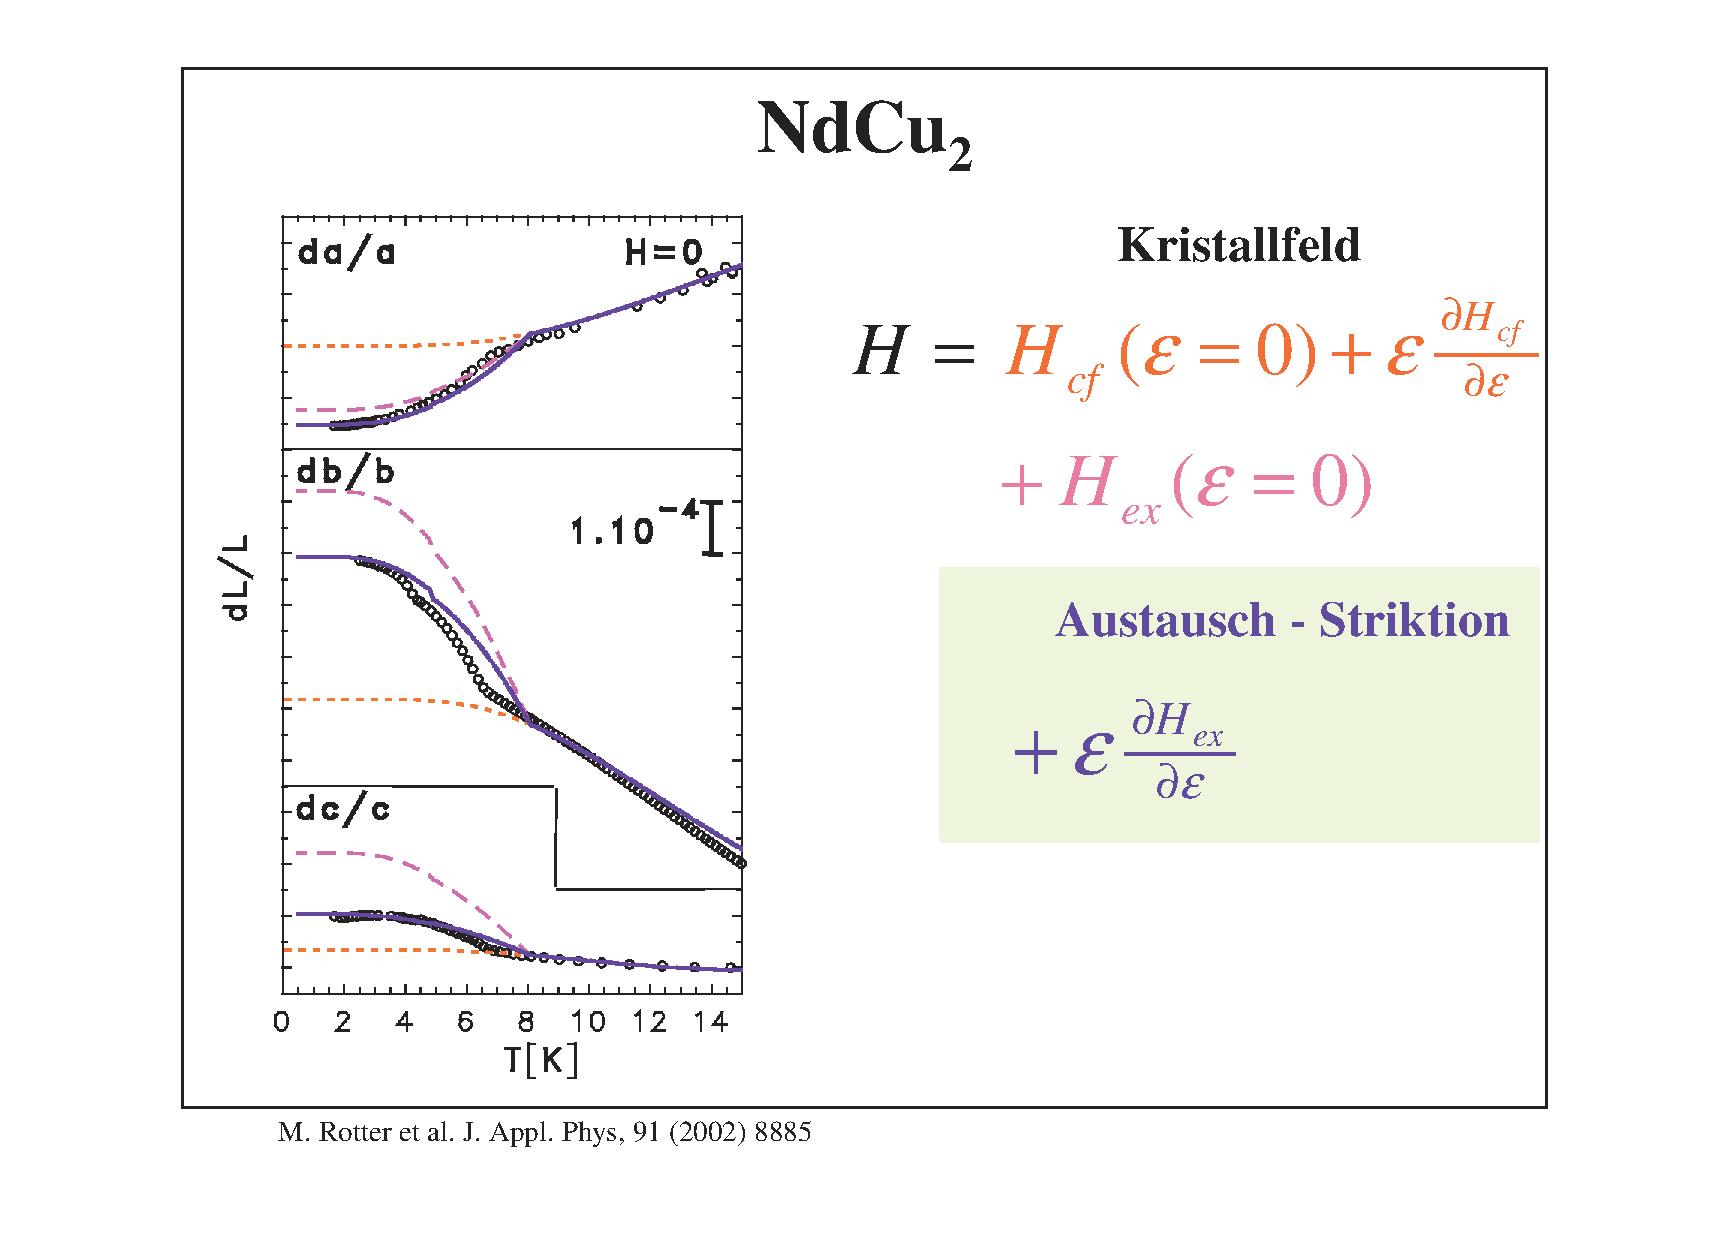
\includegraphics[angle=0, width=0.8\textwidth]{figsrc/magnetostriction_ndcu2.eps}
\end{center}
\caption{Calculated spontaneous magnetostriction of NdCu$_2$.}
\label{magnetostrictiongraphic}
\end{figure}

\begin{description}
\item [\prg mcphas.qvc]    the set of test q-vectors used for calculation of free energy.
                           Components of these q vectors refer to the reciprocal lattice $\vec a^*,\vec b^*,\vec c^*$.
\item [\prg mcphas.phs]    spin-configuration table of different types of spin-configurations. 
                            Note, in case of non-orthogonal axes the convention in these tables 
                            is $mb||\vec b$, $mc||(\vec a \times \vec b)$ and $ma$ perpendicular to $mb$ and $mc$.

                           {\em Note}: 
                           there is no natural criteria for deciding, if one spin-configuration is
			   different from another one. Therefore the list of ''different''
			   spin-configurations is dependent on the meaning of ''different''.
			   
			   The program {\prg McPhase} decides whether a spin-configuration is
			   different from another by a simple criteria, namely by the
			   angle between the spins. Comparing two spin configurations it calculates
			   the angle between corresponding spins and if for one spin the
			   angle is not small, the configuration is treated as a different
			   configuration. Therefore for example a ferromagnet with moments
			   in $a$ has a different spin configuration than a ferromagnet with
			   moments in $b$ direction. 
\item [\prg mcphas.sps]    $T-H$ dependence of spin-configuration. The spin configurations stored in this
                           file may be displayed using the program {\prg spins\index{spins}}, an example is given
			   in figure~\ref{spingraphic}.
                            Note, in case of non-orthogonal axes the convention for applied field $Ha, Hb,Hc$ and
                            also for the moment components $ma, mb, mc$ in these tables 
                            is $mb||\vec b$, $mc||(\vec a \times \vec b)$ and $ma$ perpendicular to $mb$ and $mc$.

\item [\prg mcphas.mf]     $T-H$ dependence of exchange field configuration, stored as $g_J \mu_B H_{xc}(i)$(unit is in meV)
                            for i=1,2,...,number of spins in magnetic unit cell.
                            Note, in case of non-orthogonal axes the convention for applied field $Ha, Hb,Hc$ and
                            also for the mean field components in these tables 
                            is $Hb||\vec b$, $Hc||(\vec a \times \vec b)$ and $Ha$ perpendicular to $Hb$ and $Hc$.
\item [\prg mcphas.fum]    free energy, magnetic energy (the derivative with respect to temperature gives the specific %%@
heat),
                           magnetisation data and (if cfield is used with higher order interactions)
                           expectation values of the Stevens Operators $<O_l^m>$ . As an example for the information
			   contained in this file the calculated magnetisation and magnetostriction of NdCu$_2$ is shown in
			   figures~\ref{magnetization} and ~\ref{magnetizationgraphic}.
                            Note, in case of non-orthogonal axes the convention for applied field $Ha, Hb,Hc$ and
                            also for the magnetisation components $ma,mb,mc$ in these tables 
                            is $Hb||\vec b$, $Hc||(\vec a \times \vec b)$ and $Ha$ perpendicular to $Hb$ and $Hc$.

\item [\prg mcphas1.j1 .j1 .j2 ...] 
               spin-spin correlation functions for sub-lattice 1 neighbour 1 2 ...
	       (linear combination is proportional to magnetostriction)
	       The spin-spin correlation functions for neighbour $k$ are defined by
	       the following sum of dyadic products:

	       \begin{equation}
	        \frac{1}{n}\sum_{s=1}^n <{\mbf J}^s> \times  <{\mbf J}^{s+k}>
	       \end{equation}
	       with $n$ being the number of moments in the magnetic unit cell.
	       Single ion and two-ion magnetostriction can be calculated using the $<O_l^m>$ and the
	       spin-spin correlation functions. As an example the magnetostriction analysis of
	       NdCu$_2$ is shown in figure~\ref{magnetostrictiongraphic}. For details 
             please refer to~\cite{rotter02-8885}.
                            Note, in case of non-orthogonal axes the convention for applied field $Ha, Hb,Hc$ and
                            also for the moment components in these tables 
                            is $Hb||\vec b$, $Hc||(\vec a \times \vec b)$ and $Ha$ perpendicular to $Hb$ and $Hc$.
\item [\prg mcphas.xyt]    phase diagram as x,y,T, H, phase-number j according to spin-configuration table
               given in mcphas.phs, a periodicity key, nettomoments <J>.
 Figure~\ref{phasediagramgraphic}
	       shows the phase diagram of NdCu$_2$ for magnetic fields parallel to the orthorhombic $b$-direction.
                            Note, in case of non-orthogonal axes the convention for applied field $Ha, Hb,Hc$ 
                             in these tables 
                            is $Hb||\vec b$, $Hc||(\vec a \times \vec b)$ and $Ha$ perpendicular to $Hb$ and $Hc$.
\item [\prg mcphas.hkl]    calculated (unpolarised) neutron diffraction data (the calculated magnetic intensities
    correspond to the magnetic structure + Polarisation factor. The
    Lorentz-factor , magnetic form factor and  instrumental corrections are not calculated.)
 As an example figure~\ref{neutintgraphic}
    shows the calculated temperature dependence of magnetic amplitudes for NdCu$_2$.
                           $h,k,l$ refer to the reciprocal lattice $\vec a^*,\vec b^*,\vec c^*$.
                            Note, in case of non-orthogonal axes the convention for applied field $Ha, Hb,Hc$ 
                             in these tables 
                            is $Hb||\vec b$, $Hc||(\vec a \times \vec b)$ and $Ha$ perpendicular to $Hb$ and $Hc$.
    
\item [\prg mcphasa.hkl]    Fourier Transform of the $a$-component of the magnetic Moments.
                           $h,k,l$ refer to the reciprocal lattice $\vec a^*,\vec b^*,\vec c^*$.
                            Note, in case of non-orthogonal axes the convention for applied field $Ha, Hb,Hc$ and
                            the magnetic moment component in these tables 
                            is $Hb||\vec b$, $Hc||(\vec a \times \vec b)$ and $Ha$ perpendicular to $Hb$ and $Hc$.
\item [\prg mcphasb.hkl]    Fourier Transform of the $b$-component of the magnetic Moments.
                           $h,k,l$ refer to the reciprocal lattice $\vec a^*,\vec b^*,\vec c^*$.
                            Note, in case of non-orthogonal axes the convention for applied field $Ha, Hb,Hc$ and
                            the magnetic moment component in these tables 
                            is $Hb||\vec b$, $Hc||(\vec a \times \vec b)$ and $Ha$ perpendicular to $Hb$ and $Hc$.
\item [\prg mcphasc.hkl]    Fourier Transform of the $c$-component of the magnetic Moments.
                           $h,k,l$ refer to the reciprocal lattice $\vec a^*,\vec b^*,\vec c^*$.
                            Note, in case of non-orthogonal axes the convention for applied field $Ha, Hb,Hc$ and
                            the magnetic moment component in these tables 
                            is $Hb||\vec b$, $Hc||(\vec a \times \vec b)$ and $Ha$ perpendicular to $Hb$ and $Hc$.
\end{description} 

\vspace{1cm}
{\em Exercises:}
\begin{itemize}
\item Look at the output files of {\prg McPhase}  in the directory
{\prg examples/ndcu2b\_new/results}.  At which magnetic field
the ferromagnetically aligned state is achieved (at $T=$2~K)?
\item
What is the propagation vector in the different antiferromagnetic phases at $T=$2~K ?
\end{itemize}





\subsubsection{{\prg mcphas.j\index{mcphas.j}} - lattice and exchange parameters}\label{mcphasj}
This file provides the information about 
the crystallographic
 structure and the magnetic exchange interactions.
For every atom in the crystallographic basis there
has to be given the coordinates, the number of neighbours to be considered, the 
Land\'e factor $g_J$, the single ion property filename and  a set of exchange parameters.
If the exchange parameters (and neighbour positions) are not known for your system, you 
can use the program module {\prg makenn\index{makenn}} (see section \ref{addprog}) to generate 
a list of nearest neighbours and
exchange parameters, currently implemented in {\prg makenn\index{makenn}} are dipolar interactions,
exchange interactions via the Bethe-Slater curve or the RKKY model. Note that in order
to use {\prg makenn\index{makenn}} you have to set up a working {\prg mcphas.j\index{mcphas.j}} file, which may or
may not contain neighbours and interactions.

Use program {\prg addj\index{addj}} to add exchange parameter set stored in different 
such {\prg .j} files (see section~\ref{addprog}).



\begin{description}
\item [Line 1,2:] Comment Lines
\item [Line 3:] lattice constants a,b,c and crystal angles alpha, beta, gamma 
\item [Line 4-6:] primitive lattice vectors
\item [Line 7:] Number of atoms in the primitive crystallographic unit cell ({\prg nofatoms})
\item [Line 8:] a comment line with stars
\item [Line 9:] coordinates  ($d_a$,$d_b$,$d_c$) of 1$^{st}$ magnetic ion in the crystallographic unit cell  with
respect to the lattice vectors $\vec a$,$\vec b$,$\vec c$. The number of neighbours of this 
ion, for which interaction constants are given in the interaction table (nofneighbours). 
If {\prg diagonalexchange}
is set to 0 the 9 components of the exchange tensor are given in column 4-12. 
If {\prg diagonalexchange}
 is 1, only 3 components are given (column 4-6).
If {\prg diagonalexchange}
 is 2, specific components of the exchange tensor can be given in columns 4 onwards. The indices of these components
 must be given in the following line (Line 9a below).
The Land\'e factor of the ion (gJ) and the file name of the corresponding single ion
parameter file (cffilename).
\item [Line 9a:]  If {\prg diagonalexchange=2}, then this line gives the indices of the exchange tensor corresponding to 
 the columns 4 onwards. It must have a variable called {\prg indexexchange} followed by a list of names of components of the interaction
 tensor separated by space. E.g.
 \verb|  #! indexexchange= JaJb JbJc  | 
means column 4 gives the the interaction constant between the
 first angular momentum component of the current ion with the second angular momentum component of its neighbour, whilst 
 column 5 has the interaction constant between the second angular momentum component of this ion with the third component of its
 neighbour. Alternatively, pairs of numbers may be given, as in \verb|  #! indexexchange= 1,2 2,3  |
 Additionally another parameter {\prg symmetricexchange} can be set to 1, where the value in each column is also used 
 for the transposed tensor component. Thus \verb|  #! symmetricexchange=1 indexexchange= JaJb  | is the same as \\
 \verb|  #! indexexchange= JaJb JbJa  | where the 4th and 5th column are the same.
\item [Line 10:]  Comment line
\item [Line 11-(10+nofneighbours):] Interaction table for ion number 1.   
Note: the neighbour coordinates (column 1-3) are given with respect to the lattice vectors
$\vec a$,$\vec b$,$\vec c$. The program then calculates from these values the coordinates
with respect to the primitive lattice $\vec r_1$,~$\vec r_2$,~$\vec r_3$.
($ d_a \vec a + d_b \vec b + d_c \vec c = d_1 \vec r_1 + d_2 \vec r_2 + d_3 \vec r_3$).
Column 4,5,6 \dots contain the components of the interaction tensor $\stackrel{=}{\mathcal J}$. 
Note that in case of non-orthogonal axes the 
components of the moments and the interaction tensor $Ja, Jb, Jc, Jaa, Jbb, Jcc, Jab ...$ 
refer to the orthogonal coordinate system
defined with respect to the nonorthogonal lattice $\vec a,\vec b,\vec c$ as
$Jb||\vec b$, $Jc||(\vec a \times \vec b)$ and $Ja$ perpendicular to $Jb$ and $Jc$.
\item [Line (11+nofneighbours) - end:] for each ion in the unit cell line 8 - (10+nofneighbours)
are repeated.
\end{description}


\vspace{0.5cm}

{\small {\bf Information for experienced users:}
\begin{description}
\item[\prg mcphas.jjj:]
format of exchange parameter file, which only needs a reduced set of exchange
parameters in the input file. Using the program {\prg jjj2j} the file can be transformed
to {\prg mcphas.j\index{mcphas.j}} by adding lines for all the equivalent neighbours. The format definition
of {\prg mcphas.jjj} is the same as {\prg mcphas.j\index{mcphas.j}}, however each line denotes several
equivalent neighbour atoms (instead of only one in {\prg mcphas.j\index{mcphas.j}}) according to the
 following rules:
\begin{itemize}
\item If a nonzero coordinate $d_a$ (or $d_b$,$d_c$) in the interaction table
 corresponds to it's value at the nearest
 lattice point of the primitive lattice,
  additional interactions of the same size
with  neighbours with coordinate $-d_a$ (or $-d_b$,$-d_c$, respectively)
are taken into account. This
holds for each of the three coordinates $d_a$,$d_b$ and $d_c$
 resulting in a maximum
number of 8 equivalent neighbours per line in the interaction table.
\item If the value of $d_a$ (or $d_b$,$d_c$) is zero or differs
from it's value at the nearest lattice point of the primitive lattice, it is 
changed to the value at the nearest lattice point and {\bf no} interaction 
with  neighbours with coordinates $-d_a$ (or $-d_b$,$-d_c$) is
 taken into account. If such
 interaction is needed it may be given in a different line and may
have different magnitude. In this way also crystallographic lattices
with no mirror symmetry may be described.
\end{itemize}
\item[\prg mcphas.coq:]   exchange parameters etc [ in old format]...see examples for details, use {\prg coq2jjj} to 
transform {\prg mcphas.coq} to {\prg mcphas.jjj} format
\end{description}

}


\subsubsection{Example {\prg mcphas.j\index{mcphas.j}} file for a simple antiferromagnet}

Here are example files of a tetragonal antiferromagnet with nearest neighbour interactions, all
files are equivalent:

{\small
\begin{verbatim} 
# simple antiferromagnet 
#<!--mcphase.mcphas.j-->
#***************************************************************
# Lattice Constants (A)
#! a=4.3843 b=4.3843 c=2.4194 alpha=  90 beta=  90 gamma=  90
#! r1a=   1 r2a=   0 r3a=   0
#! r1b=   0 r2b=   1 r3b=   0   primitive lattice vectors [a][b][c]
#! r1c=   0 r2c=   0 r3c=   1
#! nofatoms=1  nofcomponents=3  number of atoms in primitive unit cell/number of components of each spin
# ****************************************************************************
#! da=  0 [a] db=  0 [b] dc=  0 nofneighbours=2 diagonalexchange=0 gJ=0.857143 cffilename=Ce3p.sipf
# da[a] db[b] dc[c] Jaa[meV] Jbb[meV] Jcc[meV] Jab[meV] Jba[meV] Jac[meV] Jca[meV] Jbc[meV] Jcb[meV]
+0	+0	+1	-0.1	-0.1	-0.1   0  0  0  0  0  0
+0	+0	-1	-0.1	-0.1	-0.1   0  0  0  0  0  0
#\end{verbatim}
}

Using diagonalexchange this may be shortened to

{\small
\begin{verbatim} 
# simple antiferromagnet 
#<!--mcphase.mcphas.j-->
#***************************************************************
# Lattice Constants (A)
#! a=4.3843 b=4.3843 c=2.4194 alpha=  90 beta=  90 gamma=  90
#! r1a=   1 r2a=   0 r3a=   0
#! r1b=   0 r2b=   1 r3b=   0   primitive lattice vectors [a][b][c]
#! r1c=   0 r2c=   0 r3c=   1
#! nofatoms=1  nofcomponents=3  number of atoms in primitive unit cell/number of components of each spin
# ****************************************************************************
#! da=  0 [a] db=  0 [b] dc=  0 nofneighbours=2 diagonalexchange=1 gJ=0.857143 cffilename=Ce3p.sipf
# da[a] db[b] dc[c] Jaa[meV] Jbb[meV] Jcc[meV] Jab[meV] Jba[meV] Jac[meV] Jca[meV] Jbc[meV] Jcb[meV]
+0	+0	+1	-0.1	-0.1	-0.1   
+0	+0	-1	-0.1	-0.1	-0.1   
#\end{verbatim}
}

with indexexchange option the sequence of two ion interaction parameters can be changed and
zero parameters may be omitted:

{\small
\begin{verbatim} 
# simple antiferromagnet 
#<!--mcphase.mcphas.j-->
#***************************************************************
# Lattice Constants (A)
#! a=4.3843 b=4.3843 c=2.4194 alpha=  90 beta=  90 gamma=  90
#! r1a=   1 r2a=   0 r3a=   0
#! r1b=   0 r2b=   1 r3b=   0   primitive lattice vectors [a][b][c]
#! r1c=   0 r2c=   0 r3c=   1
#! nofatoms=1  nofcomponents=3  number of atoms in primitive unit cell/number of components of each spin
# ****************************************************************************
#! da=  0 [a] db=  0 [b] dc=  0 nofneighbours=2 diagonalexchange=2 gJ=0.857143 cffilename=Ce3p.sipf
# da[a] db[b] dc[c] Jaa[meV] Jbb[meV] Jcc[meV] Jab[meV] Jba[meV] Jac[meV] Jca[meV] Jbc[meV] Jcb[meV]
#! indexexchange = JaJa JaJc JcJa JbJb JcJc
+0	+0	+1	-0.1 0 0 -0.1	-0.1  
+0	+0	-1	-0.1 0 0 -0.1	-0.1  
#\end{verbatim}
}

{\small
\begin{verbatim} 
# simple antiferromagnet 
#<!--mcphase.mcphas.j-->
#***************************************************************
# Lattice Constants (A)
#! a=4.3843 b=4.3843 c=2.4194 alpha=  90 beta=  90 gamma=  90
#! r1a=   1 r2a=   0 r3a=   0
#! r1b=   0 r2b=   1 r3b=   0   primitive lattice vectors [a][b][c]
#! r1c=   0 r2c=   0 r3c=   1
#! nofatoms=1  nofcomponents=3  number of atoms in primitive unit cell/number of components of each spin
# ****************************************************************************
#! da=  0 [a] db=  0 [b] dc=  0 nofneighbours=2 diagonalexchange=2 gJ=0.857143 cffilename=Ce3p.sipf
# da[a] db[b] dc[c] Jaa[meV] Jbb[meV] Jcc[meV] Jab[meV] Jba[meV] Jac[meV] Jca[meV] Jbc[meV] Jcb[meV]
#! indexexchange = 1,1 1,3, 3,1 2,2 3,3
+0	+0	+1	-0.1 0 0 -0.1	-0.1  
+0	+0	-1	-0.1 0 0 -0.1	-0.1  
#\end{verbatim}
}


using symmetricexchange together with indexexchange will assume that the interaction tensor is symmetic and 
only half of it may be given:

{\small
\begin{verbatim} 
# simple antiferromagnet 
#<!--mcphase.mcphas.j-->
#***************************************************************
# Lattice Constants (A)
#! a=4.3843 b=4.3843 c=2.4194 alpha=  90 beta=  90 gamma=  90
#! r1a=   1 r2a=   0 r3a=   0
#! r1b=   0 r2b=   1 r3b=   0   primitive lattice vectors [a][b][c]
#! r1c=   0 r2c=   0 r3c=   1
#! nofatoms=1  nofcomponents=3  number of atoms in primitive unit cell/number of components of each spin
# ****************************************************************************
#! da=  0 [a] db=  0 [b] dc=  0 nofneighbours=2 diagonalexchange=2 gJ=0.857143 cffilename=Ce3p.sipf
# da[a] db[b] dc[c] Jaa[meV] Jbb[meV] Jcc[meV] Jab[meV] Jba[meV] Jac[meV] Jca[meV] Jbc[meV] Jcb[meV]
#! symmetricexchange=1 indexexchange = JaJa JaJc JbJb JcJc
+0	+0	+1	-0.1 0  -0.1	-0.1  
+0	+0	-1	-0.1 0  -0.1	-0.1  
#\end{verbatim}
}


\subsubsection{Single Ion Property Input Files}\label{sifile}

In order to speed up calculations or treat special problems a large 
variety of single ion modules is available. This includes the
option to load a user written single ion module. Details are 
given in chapter~\ref{simod}.

The first time user of {\prg McPhase} should use the module {\prg so1ion}\index{so1ion} and 
create an appropriate single ion property input file as described in
section \ref{cf1ion}. A good starting point are several examples
given in directory {\prg examples}.


\subsubsection{Example single ion property file  for a simple antiferromagnet}

Here is an example file {\prg mcphas.cf1} describing the anisotropy of a 
simple antiferromagnet with Ce atoms having basal plane anisotropy. Note the
axis convention xyz$||$abc, in case of non-orthogonal axes the convention 
is $y||\vec b$, $z||(\vec a \times \vec b)$ and $x$ perpendicular to $y$ and $z$.


\section{{\prg mcphas} - calculation of thermodynamic properties (Magnetisation, Susceptibility, Specific Heat, Neutron %%@
Diffraction, etc.)}
\label{runmcphas}

In order to perform calculations beyond the capabilities of {\prg cfield\index{cfield}} it is necessary
to use the program {\prg mcphas}. 
\begin{itemize}
\item As a first step it is possible to
calculate the thermodynamic properties such as magnetisation or specific heat
considering only single ion effects. In this case all the exchange parameters
have to be set to zero in {\prg mcphas.j\index{mcphas.j}}. 
\item for more advanced calculations the two - ion interactions have to be
considered and may lead to magnetic order. {\prg mcphas} can perform 
calculations in the ordered state in the following way: for 
a given temperature $T$ and magnetic field $\mbf H$ (vector)
several possible magnetic structures are stabilised
by a mean field algorithm and the free energy is 
calculated. The initial values for this mean-field procedure are
modified by a Monte Carlo process.


The temperature and magnetic field is varied during the calculation
and thereby it is possible to map out the magnetic phase diagram.
\end{itemize}

The program produces a plot of the stabilised magnetic
structures and the magnetisation on screen, the
output files contain additional information 
such as calculated magnetoelastic and  neutron-scattering
data. Several graphic programs easy the visualisation of the
calculated data (section~\ref{graphics}).



\subsection{Input Files}
The program {\prg McPhase} needs the following input files (all in the same directory)
 in order to run:

\begin{enumerate}
\item {\prg mcphas.ini\index{mcphas.ini}}
 - controlling the algorithm
\item {\prg mcphas.j\index{mcphas.j}}
  - lattice and exchange parameters
\item {\prg mcphas.tst\index{mcphas.tst}(optional)}  - test spin configurations
\item {\prg single-ion property files}
\item {\prg directory ./results/}
 - directory where calculated data is stored
\item {\prg directory ./fit} - experimental data for fit (optional)
\end{enumerate}


 All
 of these input files have to be in one directory and the program
has to be started in this directory. The results of the simulation
are then stored in the  subdirectory ./results/, which must exist before starting
the program 
... see directory ./examples/ for some examples.
 In order to prepare these files
for a new calculation it is best to take them from an example, copy the files
to a new directory and make the
modifications  to adapt them to the new problem.

\subsubsection{Example - a simple antiferromagnet}

In the following description of the input files we will always refer
to a simple example: a simple antiferromagnet
on a primitive orthorhombic lattice. The first time user
will thus have a simple example to follow, all corresponding
files are given in the directory {\prg tutorial/03magnetic\_phases\_mcphas/simpleAF}.
 

\subsubsection{{\prg mcphas.ini\index{mcphas.ini}} - controlling the algorithm}
   Initial file containing algorithm control parameters, for instance the range and spacing of
   propagation vectors Q or the number of Monte Carlo trials for initial spin configurations
    - {\em mind}: this
   file is rewritten and reread  when running the program and may be changed by the
   user in order to manipulate the running simulation.

{\prg mcphas.ini\index{mcphas.ini}} consists of several sections:
\begin{description}
\item [MCPHASE RUNTIME CONTROL:] this section contains the parameters
controlling the status of the calculation.
\item [XY PHASEDIAGRAM PARAMETERS:] here the temperature and field range and
step widths of the calculation are specified.
The definition of the x and y
axis in terms of temperature and magnetic field is followed by the
corresponding range and step width. An offset may be given for all
field and temperature values.
Note that for most cases of interest
this offset is zero (T0=0, Ha0=0, Hb0=0, Hc0=0).
 For the simple case of calculating a Temperature-Field phase diagram
 It is just necessary to set xT=1 and give the temperature range by
xmin/xmax/xstep. For field in b direction then just set yHb=1 and 
define the range in ymin/ymax/ystep.
In case of non-orthogonal axes the applied magnetic field
components $Ha, Hb, Hc$ refer to the orthogonal coordinate system
defined with respect to the nonorthogonal lattice $\mbf a,\mbf b,\mbf c$ as
$Hb||\mbf b$, $Hc||(\mbf a \times \mbf b)$ and $Ha$ perpendicular to $Hb$ and $Hc$.

\item [GENERATION OF SPINCONFIGURATIONS:] at the beginning of the program
some initial values of spin configurations are generated from a set of 
propagation vectors. This section defines the range of propagation vectors
and the step width.
Depending on the value of the propagation Q with respect to the primitive reciprocal lattice
1-, 2- or 3-dimensional simulations of magnetic lattices
are possible. It is advisable to 
think carefully about the chosen range and spacing of Q vectors in order
to limit calculation time.
 
For example a good starting point is to begin with a calculation with large
step widths (e.g. 0.1)  covering the Brillouin zone. This should give an idea
of the propagation vectors which are stabilised. An advanced calculation
could then fine tune the propagation and determine its accurate value (using
small step widths in a limited area of the zone).
The verbose option of {\prg mcphas} allows to inspect the propagation vectors
which are actually used in the calculation.
Trick: in order to get a quick overview of the
q-vector range covered by the mcphas\index{mcphas} simulation start mcphas, exit and 
just type {\prg felog ./results/mcphas.qvc} (need {\prg perl,perldl,pdl,pgplot} packages).

In order to limit calculation time, the maximum periodicity
of the magnetic unit cell with respect to the crystallographic unit cell 
(maxqperiod) and the maximum number of spins in the magnetic unit cell 
(maxnofspins) can be limited. Also the maximum number of test spin configurations
in the internal table can be limited (maxnoftestspincf).
A critical feature with respect to calculation time is also the number of
spin configurations which are generated by a random process from a tabulated
SPINCONFIGURATIONS during the calculation. 

In summary the variables in this section are mainly important to adapt the
program to a given computer system with finite speed. They have to be set
to optimise between speed and accuracy of the calculation. In order to
find appropriate values it is best to perform some calculations 
and restrict the parameters step by step if insufficient speed is obtained.
Also the examples included in the program package may serve as starting
points.

\item [PARAMETERS FOR SUB FECALC SELFCONSISTENCY PROCESS:] the most important
procedure in the module {\prg mcphas} is the sub fecalc. In this part of the 
program the self consistent calculation of the magnetic moment configuration
is performed as shown schematically in fig.~\ref{fecalc}. 
In the mean field approximation the Hamiltonian~(\ref{hamilton}) is approximated
by

\begin{equation}
 {\mathcal H}=\sum_n H_{SI}^n + E_{corr}
\end{equation}

with the single ion Hamiltonian (in case of module {\prg so1ion\index{so1ion}})

\begin{equation}
H_{SI}^n=  B_l^m O_{lm}({\mbf J}^n) 
	     - g_{Jn} \mu_B {\mbf J}^n {\mbf H^n_{eff}} 
\end{equation}

and the correction term

\begin{equation}
E_{corr}=\frac{1}{2}\sum_{n} g_{Jn} \mu_B \langle {\mbf J}^n
 \rangle (\mbf H^n_{eff}-\mbf H) 
\end{equation}

and with the mean fields $ \mbf H^n_{eff}$ given by

\begin{equation}\label{meanfield}
\mbf H^n_{eff}=\mbf H + \mbf H^n_{xc}=\mbf H+\sum_{{\mbf G'}n'} \frac{{\mathcal J}
(\mbf r_n-(\mbf G'+\mbf r_{n'}))}{g_{Jn}\mu_B } \langle{\mbf
J}^{n'}\rangle
\end{equation}

These mean fields and the moments $\langle \mbf J^n \rangle$ 
are determined in a self consistent
way. For a given magnetic unit cell and initial configuration 
of magnetic moments
the mean fields are calculated according to equation~(\ref{meanfield}). 
Then, for each
magnetic ion the single ion property module is taken 
and the magnetic moment $\langle \mbf J^n \rangle$ is 
calculated from it's mean field. The mean fields are used again in equation~(\ref{meanfield})
and so on .... until convergence is reached. 
Then, the free energy ($f=-kT\sum_n \ln(z_n) + E_{corr}$ ) 
of the stabilised
configuration is calculated (this is why this sub is called {\prg fecalc}). 
The free energies of a lot of different stabilised configurations have to
be compared in order to find out which configuration has lowest free energy, i.e.
is stable in thermal  equilibrium.

It may happen that this process does
not converge due to bad choice of the initial configuration, therefore a maximum number
of mean field loops has to be given by the user.
The results of a calculation may be significantly influenced by
changing parameters such as the maximum number of iteration loops 
in this section. 
In fact the simulation is always a compromise of calculation time and accuracy: if only
a few initial spin configurations are tried at each (H-T) point, the calculation speed is
fast, however it is possible that the program misses the magnetic structure with the
lowest free energy. The same holds if other critical parameters of the simulation are
restricted too much.
 

\item [OUTPUT OF PHYSICAL PROPERTIES:]
Some options for the output of the calculation can be changed in this section.
\end{description}

\begin{figure}[hb]
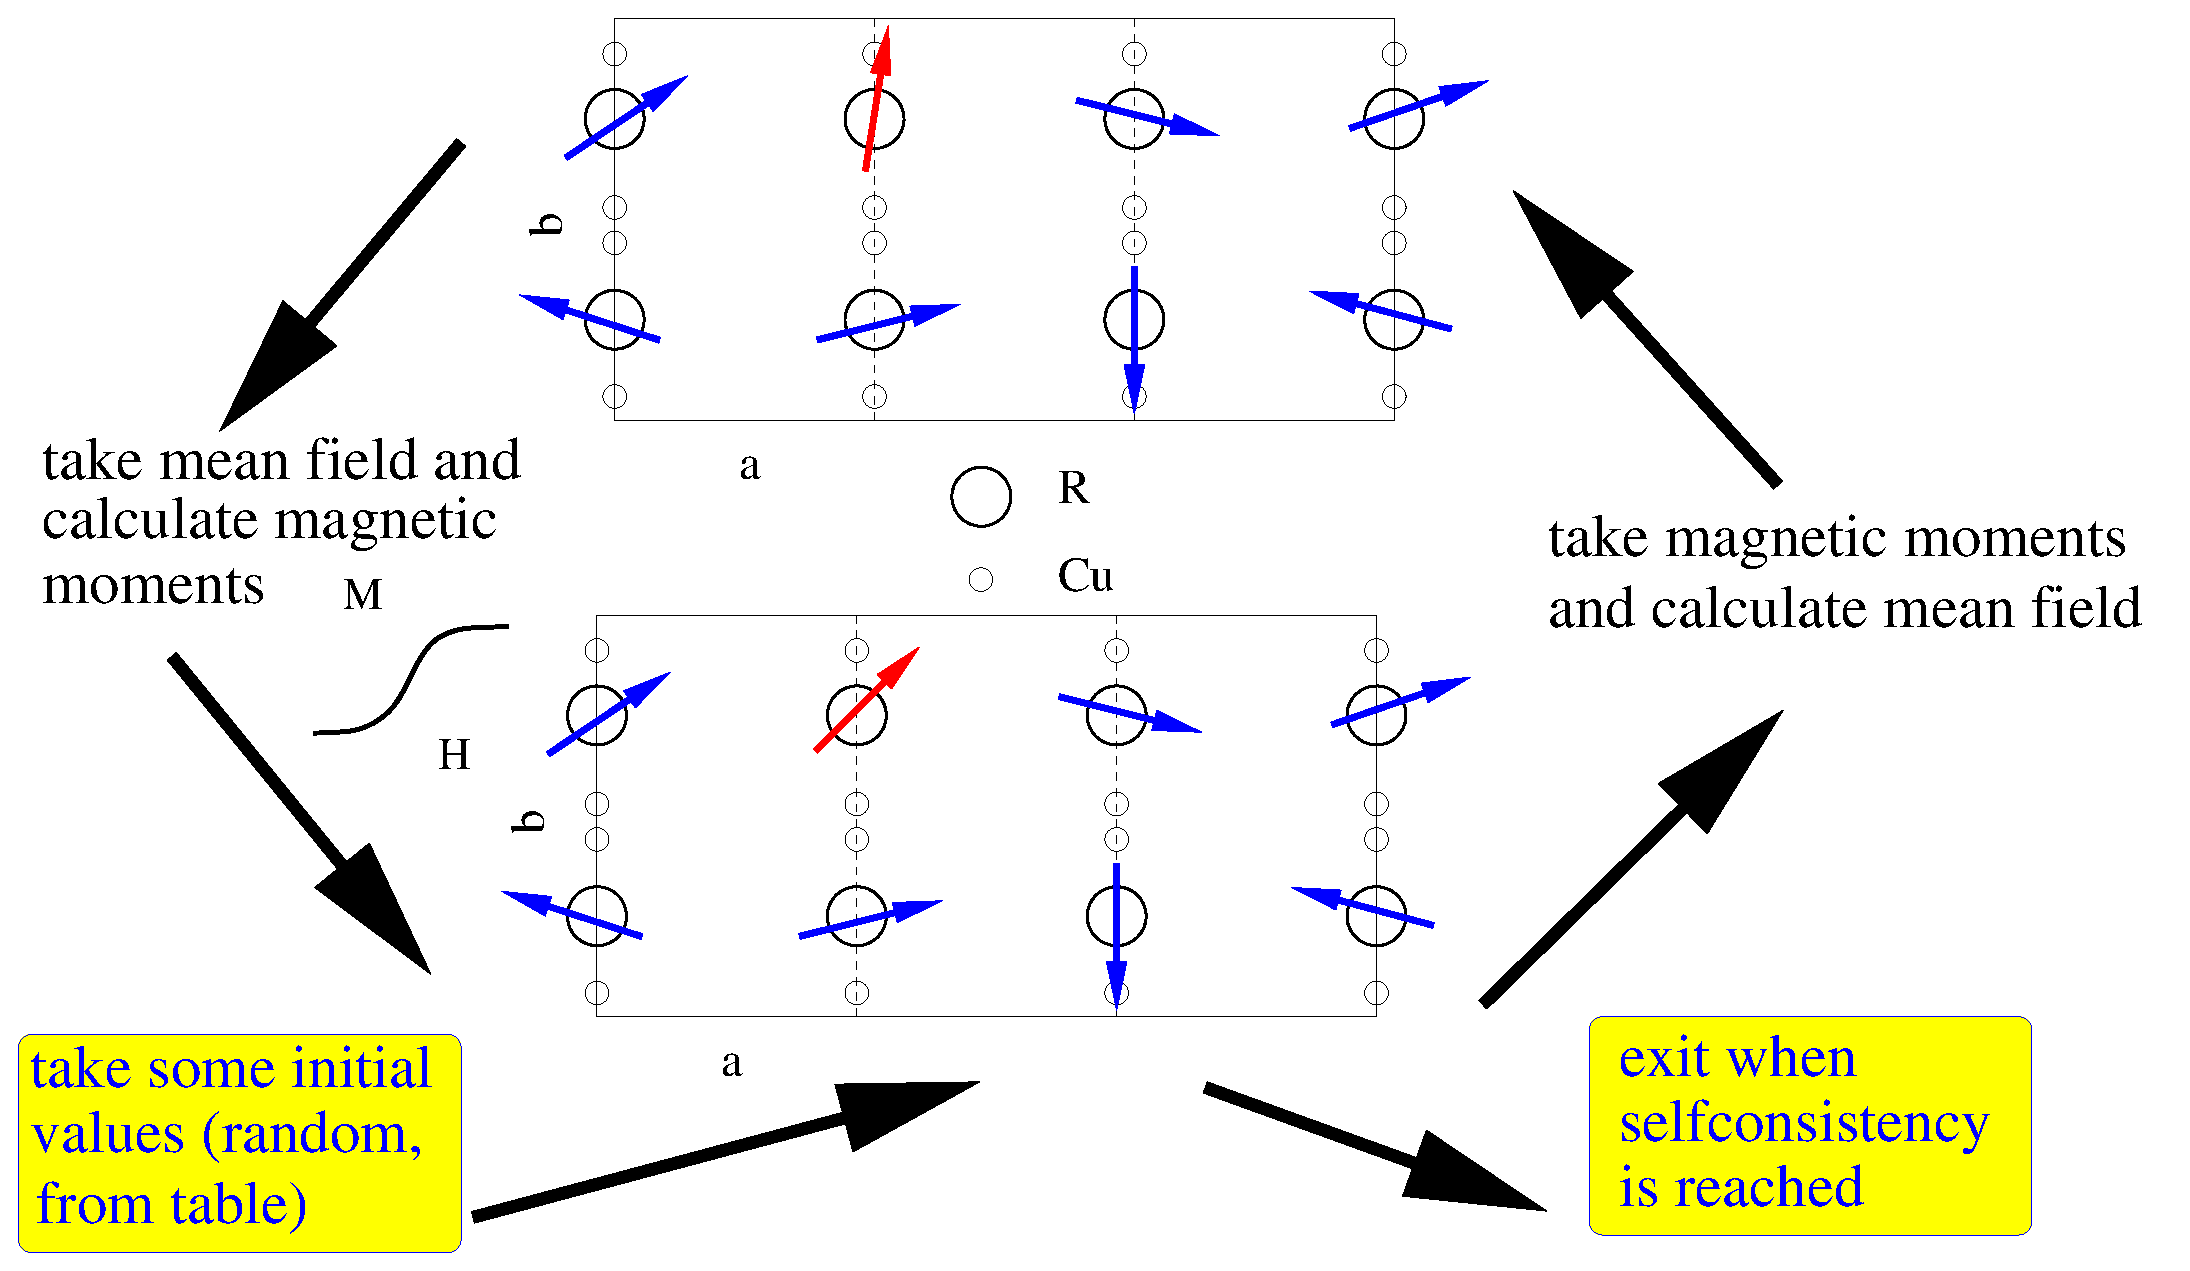
\includegraphics[angle=0,width=0.9\columnwidth]{figsrc/fecalc.eps}
\caption{\label{fecalc}Mean field process of sub {\prg fecalc}.}
\end{figure}

 
\subsubsection{Example {\prg mcphas.ini\index{mcphas.ini}} file for a simple antiferromagnet}

Here is an example of {\prg mcphas.ini\index{mcphas.ini}}, the comments describe the meaning of the different
parameters:

\input{mcphas.ini}



\subsubsection{{\prg mcphas.j\index{mcphas.j}} - lattice and exchange parameters}\label{mcphasj}
This file provides the information about 
the crystallographic
 structure and the magnetic exchange interactions.
For every atom in the crystallographic basis there
has to be given the coordinates, the number of neighbours to be considered, the 
Land\'e factor $g_J$, the single ion property filename and  a set of exchange parameters.
If the exchange parameters (and neighbour positions) are not known for your system, you 
can use the program module {\prg makenn\index{makenn}} (see section \ref{addprog}) to generate 
a list of nearest neighbours and
exchange parameters, currently implemented in {\prg makenn\index{makenn}} are dipolar interactions,
exchange interactions via the Bethe-Slater curve or the RKKY model. Note that in order
to use {\prg makenn\index{makenn}} you have to set up a working {\prg mcphas.j\index{mcphas.j}} file, which may or
may not contain neighbours and interactions.

Use program {\prg addj\index{addj}} to add exchange parameter set stored in different 
such {\prg .j} files (see section~\ref{addprog}).



\begin{description}
\item [Line 1,2:] Comment Lines
\item [Line 3:] lattice constants a,b,c and crystal angles alpha, beta, gamma 
\item [Line 4-6:] primitive lattice vectors
\item [Line 7:] Number of atoms in the primitive crystallographic unit cell ({\prg nofatoms})
\item [Line 8:] a comment line with stars
\item [Line 9:] coordinates  ($d_a$,$d_b$,$d_c$) of 1$^{st}$ magnetic ion in the crystallographic unit cell  with
respect to the lattice vectors $\vec a$,$\vec b$,$\vec c$. The number of neighbours of this 
ion, for which interaction constants are given in the interaction table (nofneighbours). 
If {\prg diagonalexchange}
is set to 0 the 9 components of the exchange tensor are given in column 4-12. 
If {\prg diagonalexchange}
 is 1, only 3 components are given (column 4-6).
If {\prg diagonalexchange}
 is 2, specific components of the exchange tensor can be given in columns 4 onwards. The indices of these components
 must be given in the following line (Line 9a below).
The Land\'e factor of the ion (gJ) and the file name of the corresponding single ion
parameter file (cffilename).
\item [Line 9a:]  If {\prg diagonalexchange=2}, then this line gives the indices of the exchange tensor corresponding to 
 the columns 4 onwards. It must have a variable called {\prg indexexchange} followed by a list of names of components of the interaction
 tensor separated by space. E.g.
 \verb|  #! indexexchange= JaJb JbJc  | 
means column 4 gives the the interaction constant between the
 first angular momentum component of the current ion with the second angular momentum component of its neighbour, whilst 
 column 5 has the interaction constant between the second angular momentum component of this ion with the third component of its
 neighbour. Alternatively, pairs of numbers may be given, as in \verb|  #! indexexchange= 1,2 2,3  |
 Additionally another parameter {\prg symmetricexchange} can be set to 1, where the value in each column is also used 
 for the transposed tensor component. Thus \verb|  #! symmetricexchange=1 indexexchange= JaJb  | is the same as \\
 \verb|  #! indexexchange= JaJb JbJa  | where the 4th and 5th column are the same.
\item [Line 10:]  Comment line
\item [Line 11-(10+nofneighbours):] Interaction table for ion number 1.   
Note: the neighbour coordinates (column 1-3) are given with respect to the lattice vectors
$\vec a$,$\vec b$,$\vec c$. The program then calculates from these values the coordinates
with respect to the primitive lattice $\vec r_1$,~$\vec r_2$,~$\vec r_3$.
($ d_a \vec a + d_b \vec b + d_c \vec c = d_1 \vec r_1 + d_2 \vec r_2 + d_3 \vec r_3$).
Column 4,5,6 \dots contain the components of the interaction tensor $\stackrel{=}{\mathcal J}$. 
Note that in case of non-orthogonal axes the 
components of the moments and the interaction tensor $Ja, Jb, Jc, Jaa, Jbb, Jcc, Jab ...$ 
refer to the orthogonal coordinate system
defined with respect to the nonorthogonal lattice $\vec a,\vec b,\vec c$ as
$Jb||\vec b$, $Jc||(\vec a \times \vec b)$ and $Ja$ perpendicular to $Jb$ and $Jc$.
\item [Line (11+nofneighbours) - end:] for each ion in the unit cell line 8 - (10+nofneighbours)
are repeated.
\end{description}


\vspace{0.5cm}

{\small {\bf Information for experienced users:}
\begin{description}
\item[\prg mcphas.jjj:]
format of exchange parameter file, which only needs a reduced set of exchange
parameters in the input file. Using the program {\prg jjj2j} the file can be transformed
to {\prg mcphas.j\index{mcphas.j}} by adding lines for all the equivalent neighbours. The format definition
of {\prg mcphas.jjj} is the same as {\prg mcphas.j\index{mcphas.j}}, however each line denotes several
equivalent neighbour atoms (instead of only one in {\prg mcphas.j\index{mcphas.j}}) according to the
 following rules:
\begin{itemize}
\item If a nonzero coordinate $d_a$ (or $d_b$,$d_c$) in the interaction table
 corresponds to it's value at the nearest
 lattice point of the primitive lattice,
  additional interactions of the same size
with  neighbours with coordinate $-d_a$ (or $-d_b$,$-d_c$, respectively)
are taken into account. This
holds for each of the three coordinates $d_a$,$d_b$ and $d_c$
 resulting in a maximum
number of 8 equivalent neighbours per line in the interaction table.
\item If the value of $d_a$ (or $d_b$,$d_c$) is zero or differs
from it's value at the nearest lattice point of the primitive lattice, it is 
changed to the value at the nearest lattice point and {\bf no} interaction 
with  neighbours with coordinates $-d_a$ (or $-d_b$,$-d_c$) is
 taken into account. If such
 interaction is needed it may be given in a different line and may
have different magnitude. In this way also crystallographic lattices
with no mirror symmetry may be described.
\end{itemize}
\item[\prg mcphas.coq:]   exchange parameters etc [ in old format]...see examples for details, use {\prg coq2jjj} to 
transform {\prg mcphas.coq} to {\prg mcphas.jjj} format
\end{description}

}


\subsubsection{Example {\prg mcphas.j\index{mcphas.j}} file for a simple antiferromagnet}

Here are example files of a tetragonal antiferromagnet with nearest neighbour interactions, all
files are equivalent:

{\small
\begin{verbatim} 
# simple antiferromagnet 
#<!--mcphase.mcphas.j-->
#***************************************************************
# Lattice Constants (A)
#! a=4.3843 b=4.3843 c=2.4194 alpha=  90 beta=  90 gamma=  90
#! r1a=   1 r2a=   0 r3a=   0
#! r1b=   0 r2b=   1 r3b=   0   primitive lattice vectors [a][b][c]
#! r1c=   0 r2c=   0 r3c=   1
#! nofatoms=1  nofcomponents=3  number of atoms in primitive unit cell/number of components of each spin
# ****************************************************************************
#! da=  0 [a] db=  0 [b] dc=  0 nofneighbours=2 diagonalexchange=0 gJ=0.857143 cffilename=Ce3p.sipf
# da[a] db[b] dc[c] Jaa[meV] Jbb[meV] Jcc[meV] Jab[meV] Jba[meV] Jac[meV] Jca[meV] Jbc[meV] Jcb[meV]
+0	+0	+1	-0.1	-0.1	-0.1   0  0  0  0  0  0
+0	+0	-1	-0.1	-0.1	-0.1   0  0  0  0  0  0
#\end{verbatim}
}

Using diagonalexchange this may be shortened to

{\small
\begin{verbatim} 
# simple antiferromagnet 
#<!--mcphase.mcphas.j-->
#***************************************************************
# Lattice Constants (A)
#! a=4.3843 b=4.3843 c=2.4194 alpha=  90 beta=  90 gamma=  90
#! r1a=   1 r2a=   0 r3a=   0
#! r1b=   0 r2b=   1 r3b=   0   primitive lattice vectors [a][b][c]
#! r1c=   0 r2c=   0 r3c=   1
#! nofatoms=1  nofcomponents=3  number of atoms in primitive unit cell/number of components of each spin
# ****************************************************************************
#! da=  0 [a] db=  0 [b] dc=  0 nofneighbours=2 diagonalexchange=1 gJ=0.857143 cffilename=Ce3p.sipf
# da[a] db[b] dc[c] Jaa[meV] Jbb[meV] Jcc[meV] Jab[meV] Jba[meV] Jac[meV] Jca[meV] Jbc[meV] Jcb[meV]
+0	+0	+1	-0.1	-0.1	-0.1   
+0	+0	-1	-0.1	-0.1	-0.1   
#\end{verbatim}
}

with indexexchange option the sequence of two ion interaction parameters can be changed and
zero parameters may be omitted:

{\small
\begin{verbatim} 
# simple antiferromagnet 
#<!--mcphase.mcphas.j-->
#***************************************************************
# Lattice Constants (A)
#! a=4.3843 b=4.3843 c=2.4194 alpha=  90 beta=  90 gamma=  90
#! r1a=   1 r2a=   0 r3a=   0
#! r1b=   0 r2b=   1 r3b=   0   primitive lattice vectors [a][b][c]
#! r1c=   0 r2c=   0 r3c=   1
#! nofatoms=1  nofcomponents=3  number of atoms in primitive unit cell/number of components of each spin
# ****************************************************************************
#! da=  0 [a] db=  0 [b] dc=  0 nofneighbours=2 diagonalexchange=2 gJ=0.857143 cffilename=Ce3p.sipf
# da[a] db[b] dc[c] Jaa[meV] Jbb[meV] Jcc[meV] Jab[meV] Jba[meV] Jac[meV] Jca[meV] Jbc[meV] Jcb[meV]
#! indexexchange = JaJa JaJc JcJa JbJb JcJc
+0	+0	+1	-0.1 0 0 -0.1	-0.1  
+0	+0	-1	-0.1 0 0 -0.1	-0.1  
#\end{verbatim}
}

{\small
\begin{verbatim} 
# simple antiferromagnet 
#<!--mcphase.mcphas.j-->
#***************************************************************
# Lattice Constants (A)
#! a=4.3843 b=4.3843 c=2.4194 alpha=  90 beta=  90 gamma=  90
#! r1a=   1 r2a=   0 r3a=   0
#! r1b=   0 r2b=   1 r3b=   0   primitive lattice vectors [a][b][c]
#! r1c=   0 r2c=   0 r3c=   1
#! nofatoms=1  nofcomponents=3  number of atoms in primitive unit cell/number of components of each spin
# ****************************************************************************
#! da=  0 [a] db=  0 [b] dc=  0 nofneighbours=2 diagonalexchange=2 gJ=0.857143 cffilename=Ce3p.sipf
# da[a] db[b] dc[c] Jaa[meV] Jbb[meV] Jcc[meV] Jab[meV] Jba[meV] Jac[meV] Jca[meV] Jbc[meV] Jcb[meV]
#! indexexchange = 1,1 1,3, 3,1 2,2 3,3
+0	+0	+1	-0.1 0 0 -0.1	-0.1  
+0	+0	-1	-0.1 0 0 -0.1	-0.1  
#\end{verbatim}
}


using symmetricexchange together with indexexchange will assume that the interaction tensor is symmetic and 
only half of it may be given:

{\small
\begin{verbatim} 
# simple antiferromagnet 
#<!--mcphase.mcphas.j-->
#***************************************************************
# Lattice Constants (A)
#! a=4.3843 b=4.3843 c=2.4194 alpha=  90 beta=  90 gamma=  90
#! r1a=   1 r2a=   0 r3a=   0
#! r1b=   0 r2b=   1 r3b=   0   primitive lattice vectors [a][b][c]
#! r1c=   0 r2c=   0 r3c=   1
#! nofatoms=1  nofcomponents=3  number of atoms in primitive unit cell/number of components of each spin
# ****************************************************************************
#! da=  0 [a] db=  0 [b] dc=  0 nofneighbours=2 diagonalexchange=2 gJ=0.857143 cffilename=Ce3p.sipf
# da[a] db[b] dc[c] Jaa[meV] Jbb[meV] Jcc[meV] Jab[meV] Jba[meV] Jac[meV] Jca[meV] Jbc[meV] Jcb[meV]
#! symmetricexchange=1 indexexchange = JaJa JaJc JbJb JcJc
+0	+0	+1	-0.1 0  -0.1	-0.1  
+0	+0	-1	-0.1 0  -0.1	-0.1  
#\end{verbatim}
}


\subsubsection{Single Ion Property Input Files}\label{sifile}

In order to speed up calculations or treat special problems a large 
variety of single ion modules is available. This includes the
option to load a user written single ion module. Details are 
given in chapter~\ref{simod}.

The first time user of {\prg McPhase} should use the module {\prg so1ion}\index{so1ion} and 
create an appropriate single ion property input file as described in
section \ref{cf1ion}. A good starting point are several examples
given in directory {\prg examples}.


\subsubsection{Example single ion property file  for a simple antiferromagnet}

Here is an example file {\prg mcphas.cf1} describing the anisotropy of a 
simple antiferromagnet with Ce atoms having basal plane anisotropy. Note the
axis convention xyz$||$abc, in case of non-orthogonal axes the convention 
is $y||\vec b$, $z||(\vec a \times \vec b)$ and $x$ perpendicular to $y$ and $z$.


\input{mcphas.cf1}

\subsubsection{{\prg mcphas.tst\index{mcphas.tst}} - input file of test spin-configurations (optional)}
This file is optional and contains
some test momentum configurations to be used for the calculation
             of the free energy. Mind that
\begin{itemize}
\item  in the file header the number of atoms in the primitive
       crystallographic unit cell and the number of components
       of the spin vector have to be given.
\item  at the end of the
 file there must be no empty lines !
\end{itemize}

The momentum - configurations tables always refer to spins sitting on
the primitive lattice ${\mbf r}_i$. If more than one atom is in
the primitive basis, the momentum gets $3n$ components ($n=$ number
of atoms in the crystallographic basis). See {\prg ./examples/ndcu2b\_new/} for
examples of a two atom basis. Units of these tables are that of total 
angular momentum $<J>$.

\subsubsection{Example {\prg mcphas.tst\index{mcphas.tst}} file  for a simple antiferromagnet}

Here is the file {\prg mcphas.tst\index{mcphas.tst}} for the simple antiferromagnet example
describing some spin configurations
to be used as starting values for the mean field process:

\input{mcphas.tst}
Note, in case of non-orthogonal axes the convention 
is $mb||\vec b$, $mc||(\vec a \times \vec b)$ and $ma$ perpendicular to $mb$ and $mc$.

\subsubsection{subdirectory {\prg ./results} - directory where calculated data is stored}

In order to be able to save the results of a calculation the directory {\prg ./results} has to
exist. Mind that all files in this directory will be overwritten without warning. 

\subsubsection{subdirectory {\prg ./fit} - experimental data for fit (optional) } 

In order that {\prg McPhase} can calculate the standard deviation between
 experimental data and the results of the simulation, some experimental data
 can be given in the subdirectory {\prg ./fit}. The filenames and the data-format
 are the same as the output files of {\prg McPhas}, e.g. {\prg mcphas.fum}, {\prg mcphas.hkl}
 etc. {\prg McPhase} looks into the directory {\prg ./fit} and if it finds any
 of these files, the standard deviation is increased correspondingly. 

What measurement data can be used to calculate a standard deviation ?

\begin{description}
\item[{\prg mcphas.fum}] if given in column 11, 12, 13 in {\prg ./fit/mcphas.fum} the
            magnetisation in the $a$, $b$ and $c$ direction is used for calculation
	    of the standard deviation sta. The standard deviation is calculated
	    as ${\rm sta}=\sum_{\rm data points i} ({\mbf m}_i^{calc}-{\mbf m}_i^{meas})^2$.
	    All three components of the magnetic moment have to be given and are used.

\end{description}

Note that the measured data has to be given in those (H-T) points which are 
calculated by mcphas\index{mcphas} in order to be used by the program to increase {\prg sta}.
It is usually most effective to fit only few data points, because a large set
of data points will not improve the quality of the fit and only require a large
amount of calculation time.



\subsection{Starting a simulation}
\label{start}

To start the simulation goto the directory containing the
input files {\prg mcphas.ini, mcphas.j, etc. } and type

\begin{description}
\item[\prg mcphas] to run the program generating stepwise $H-T$ values 
              in a loop given by {\prg mcphas.ini\index{mcphas.ini}} (you can also press the
              symbol in the {\prg McPhase - Explorer} window).
\item[\prg mcphas\index{mcphas} [file]]  to run the program with an input file --   
             {\prg file} contains T ha hb hc values to be calculated 
             if [file] is not given, xmin xmax xstep (xT xHa xHb xHc)
             ymin ymax ystep (yT yHa yHb yHc) is read from file {\prg mcphas.ini\index{mcphas.ini}}
	     and phase diagram is calculated
\item[\prg mcphas\index{mcphas} -h]  to  print help and version of {\prg McPhas}.
\item[\prg mcphas\index{mcphas} -stamax 14]  end mcphas\index{mcphas} if standard deviation exceeds 14.
\item[\prg mcphas\index{mcphas} -a] avoid overwriting output files in results, append new results to existing files
\item[\prg mcphas\index{mcphas} -v]  to  enable verbose mode with lots of messages of {\prg McPhas}. Specifically
the verbose mode enables the following features:
  \begin{itemize}
			          \item more information is printed out, 
			          \item the q-vectors file {\prg ./results/mcphas.qvc} will contain 
				    the explicit spin configurations
			          \item the display\index{display} on screen (ghostview window using 
				     {\prg ./results/.sps.eps}) will be updated not only 
				    when a H-T point has been finished but always 
				    when a structure with smaller free energy 
				    has been stabilised
  \end{itemize}
\item[\prg mcphasit\index{mcphas}] to start mcphase in commandline mode without opening any window
\end{description}

\vspace{1cm}
{\em Exercises:}
\begin{itemize}
\item Look at the input files for {\prg McPhase} given in the directory
{\prg examples/ndcu2b\_new}.  How many atoms are contained in the crystallographic basis ?
\item
Start the simulation by typing the command {\prg mcphas}.
\end{itemize}



\subsection{Options for a running simulation}
... when the program is running, the options in the main window
can be changed. Pressing ''displayall'' displays the current spin-configuration
at each iteration step. Pressing ''log fe vs Q'' appends free energy vs Q
data to {\prg mcphas.log} for every ($T-H$) point.


The file {\prg ./results/.spins.eps} is used to show the information about the currently calculated
spin structure on the screen using the postscript file viewer ghostview.

The file {\prg ./results/.mcphas.fum} contains the information of the magnetisation curve
which is currently calculated. This information is automatically displayed on the screen.


The program {\prg display} (see section \ref{display}) can be used 
for the online display\index{display} of any other
curve(s).


\subsection{Output Files - {\prg mcphas.qvc,phs,sps,mf,fum,j1...,xyt,hkl} }\label{outputfiles}
 (in directory ./results/ after a simulation run) 

\begin{figure}[htb]%h=here, t=top, b=bottom, p=separate figure page
\begin{center}\leavevmode
\includegraphics[angle=0, width=0.3\textwidth]{figsrc/magnetization_ndcu2.ps}
\end{center}
\caption{Calculated magnetisation of NdCu$_2$ for field parallel to the orthorhombic $b$-direction.}
\label{magnetization}
\end{figure}

\begin{figure}[htb]%h=here, t=top, b=bottom, p=separate figure page
\begin{center}\leavevmode
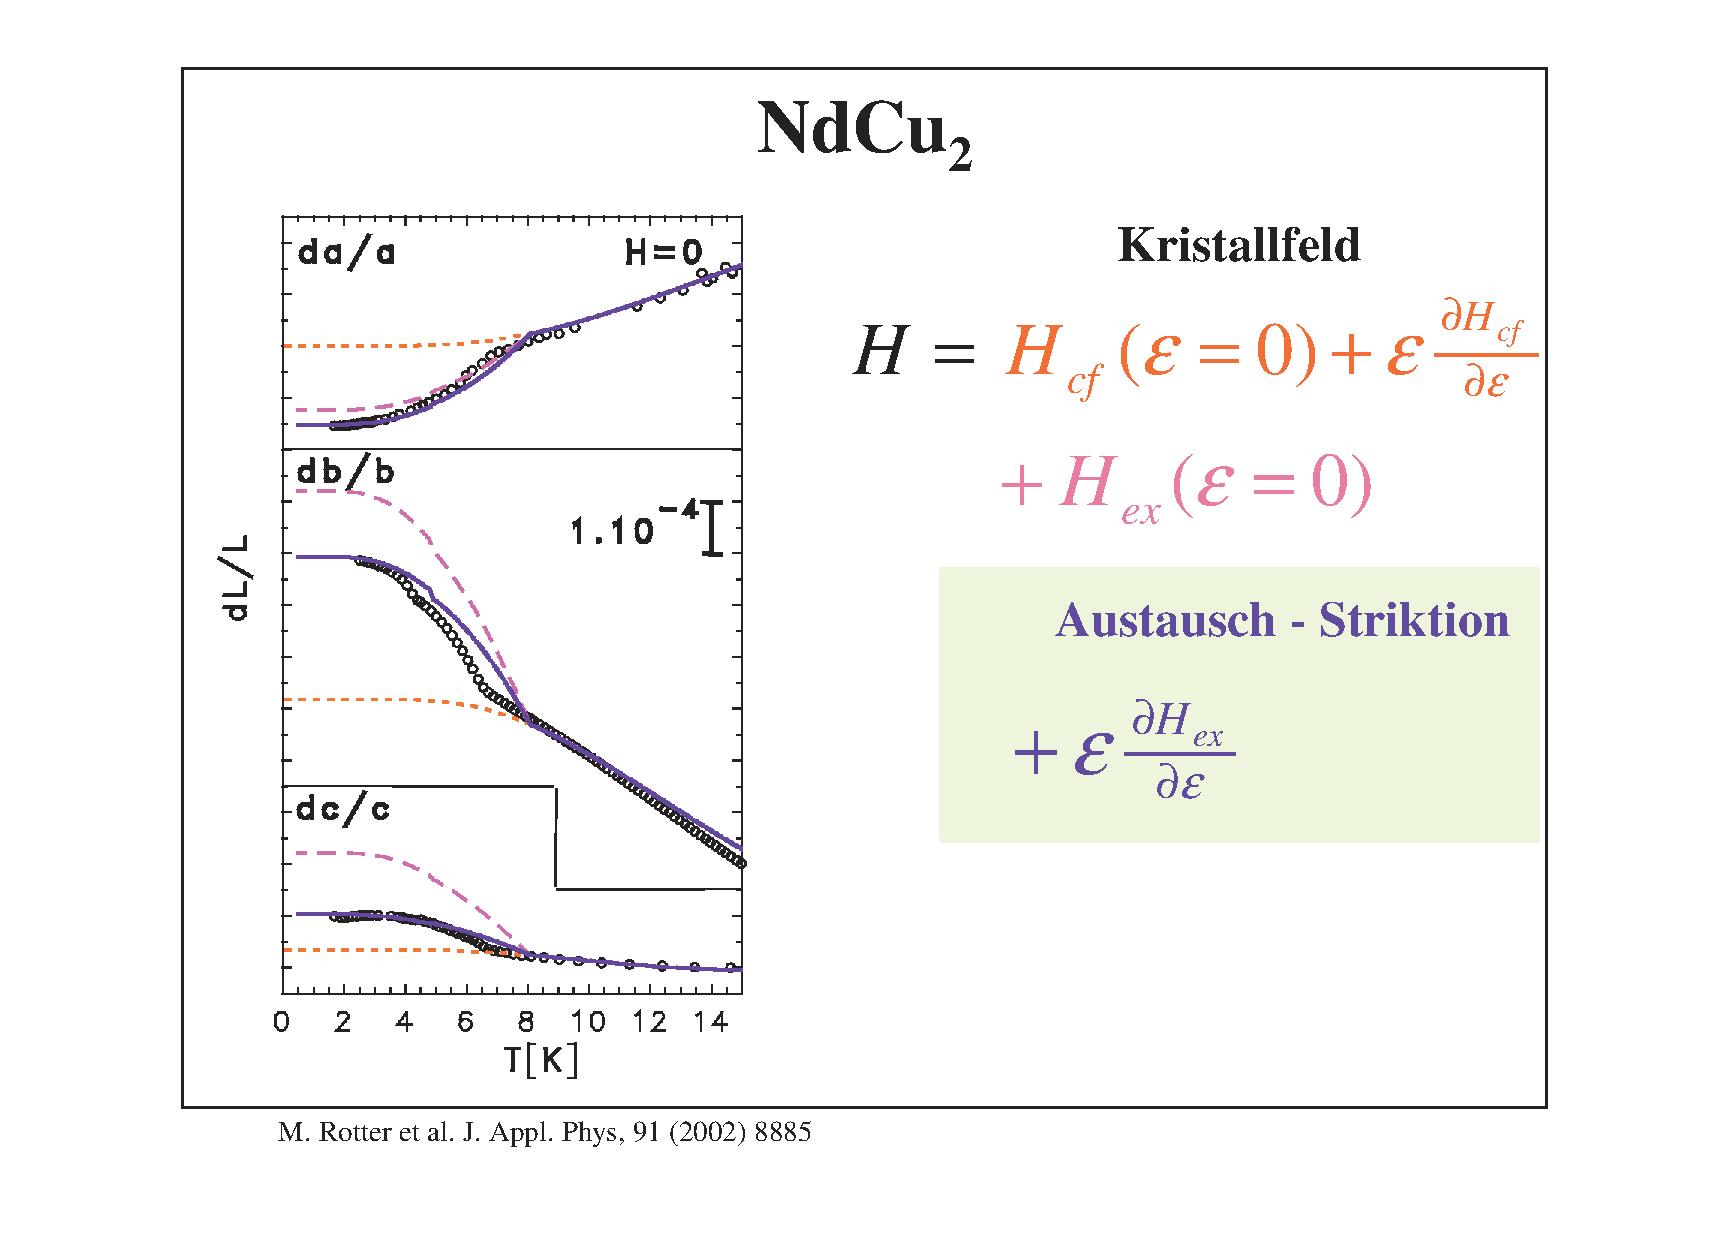
\includegraphics[angle=0, width=0.8\textwidth]{figsrc/magnetostriction_ndcu2.eps}
\end{center}
\caption{Calculated spontaneous magnetostriction of NdCu$_2$.}
\label{magnetostrictiongraphic}
\end{figure}

\begin{description}
\item [\prg mcphas.qvc]    the set of test q-vectors used for calculation of free energy.
                           Components of these q vectors refer to the reciprocal lattice $\vec a^*,\vec b^*,\vec c^*$.
\item [\prg mcphas.phs]    spin-configuration table of different types of spin-configurations. 
                            Note, in case of non-orthogonal axes the convention in these tables 
                            is $mb||\vec b$, $mc||(\vec a \times \vec b)$ and $ma$ perpendicular to $mb$ and $mc$.

                           {\em Note}: 
                           there is no natural criteria for deciding, if one spin-configuration is
			   different from another one. Therefore the list of ''different''
			   spin-configurations is dependent on the meaning of ''different''.
			   
			   The program {\prg McPhase} decides whether a spin-configuration is
			   different from another by a simple criteria, namely by the
			   angle between the spins. Comparing two spin configurations it calculates
			   the angle between corresponding spins and if for one spin the
			   angle is not small, the configuration is treated as a different
			   configuration. Therefore for example a ferromagnet with moments
			   in $a$ has a different spin configuration than a ferromagnet with
			   moments in $b$ direction. 
\item [\prg mcphas.sps]    $T-H$ dependence of spin-configuration. The spin configurations stored in this
                           file may be displayed using the program {\prg spins\index{spins}}, an example is given
			   in figure~\ref{spingraphic}.
                            Note, in case of non-orthogonal axes the convention for applied field $Ha, Hb,Hc$ and
                            also for the moment components $ma, mb, mc$ in these tables 
                            is $mb||\vec b$, $mc||(\vec a \times \vec b)$ and $ma$ perpendicular to $mb$ and $mc$.

\item [\prg mcphas.mf]     $T-H$ dependence of exchange field configuration, stored as $g_J \mu_B H_{xc}(i)$(unit is in meV)
                            for i=1,2,...,number of spins in magnetic unit cell.
                            Note, in case of non-orthogonal axes the convention for applied field $Ha, Hb,Hc$ and
                            also for the mean field components in these tables 
                            is $Hb||\vec b$, $Hc||(\vec a \times \vec b)$ and $Ha$ perpendicular to $Hb$ and $Hc$.
\item [\prg mcphas.fum]    free energy, magnetic energy (the derivative with respect to temperature gives the specific %%@
heat),
                           magnetisation data and (if cfield is used with higher order interactions)
                           expectation values of the Stevens Operators $<O_l^m>$ . As an example for the information
			   contained in this file the calculated magnetisation and magnetostriction of NdCu$_2$ is shown in
			   figures~\ref{magnetization} and ~\ref{magnetizationgraphic}.
                            Note, in case of non-orthogonal axes the convention for applied field $Ha, Hb,Hc$ and
                            also for the magnetisation components $ma,mb,mc$ in these tables 
                            is $Hb||\vec b$, $Hc||(\vec a \times \vec b)$ and $Ha$ perpendicular to $Hb$ and $Hc$.

\item [\prg mcphas1.j1 .j1 .j2 ...] 
               spin-spin correlation functions for sub-lattice 1 neighbour 1 2 ...
	       (linear combination is proportional to magnetostriction)
	       The spin-spin correlation functions for neighbour $k$ are defined by
	       the following sum of dyadic products:

	       \begin{equation}
	        \frac{1}{n}\sum_{s=1}^n <{\mbf J}^s> \times  <{\mbf J}^{s+k}>
	       \end{equation}
	       with $n$ being the number of moments in the magnetic unit cell.
	       Single ion and two-ion magnetostriction can be calculated using the $<O_l^m>$ and the
	       spin-spin correlation functions. As an example the magnetostriction analysis of
	       NdCu$_2$ is shown in figure~\ref{magnetostrictiongraphic}. For details 
             please refer to~\cite{rotter02-8885}.
                            Note, in case of non-orthogonal axes the convention for applied field $Ha, Hb,Hc$ and
                            also for the moment components in these tables 
                            is $Hb||\vec b$, $Hc||(\vec a \times \vec b)$ and $Ha$ perpendicular to $Hb$ and $Hc$.
\item [\prg mcphas.xyt]    phase diagram as x,y,T, H, phase-number j according to spin-configuration table
               given in mcphas.phs, a periodicity key, nettomoments <J>.
 Figure~\ref{phasediagramgraphic}
	       shows the phase diagram of NdCu$_2$ for magnetic fields parallel to the orthorhombic $b$-direction.
                            Note, in case of non-orthogonal axes the convention for applied field $Ha, Hb,Hc$ 
                             in these tables 
                            is $Hb||\vec b$, $Hc||(\vec a \times \vec b)$ and $Ha$ perpendicular to $Hb$ and $Hc$.
\item [\prg mcphas.hkl]    calculated (unpolarised) neutron diffraction data (the calculated magnetic intensities
    correspond to the magnetic structure + Polarisation factor. The
    Lorentz-factor , magnetic form factor and  instrumental corrections are not calculated.)
 As an example figure~\ref{neutintgraphic}
    shows the calculated temperature dependence of magnetic amplitudes for NdCu$_2$.
                           $h,k,l$ refer to the reciprocal lattice $\vec a^*,\vec b^*,\vec c^*$.
                            Note, in case of non-orthogonal axes the convention for applied field $Ha, Hb,Hc$ 
                             in these tables 
                            is $Hb||\vec b$, $Hc||(\vec a \times \vec b)$ and $Ha$ perpendicular to $Hb$ and $Hc$.
    
\item [\prg mcphasa.hkl]    Fourier Transform of the $a$-component of the magnetic Moments.
                           $h,k,l$ refer to the reciprocal lattice $\vec a^*,\vec b^*,\vec c^*$.
                            Note, in case of non-orthogonal axes the convention for applied field $Ha, Hb,Hc$ and
                            the magnetic moment component in these tables 
                            is $Hb||\vec b$, $Hc||(\vec a \times \vec b)$ and $Ha$ perpendicular to $Hb$ and $Hc$.
\item [\prg mcphasb.hkl]    Fourier Transform of the $b$-component of the magnetic Moments.
                           $h,k,l$ refer to the reciprocal lattice $\vec a^*,\vec b^*,\vec c^*$.
                            Note, in case of non-orthogonal axes the convention for applied field $Ha, Hb,Hc$ and
                            the magnetic moment component in these tables 
                            is $Hb||\vec b$, $Hc||(\vec a \times \vec b)$ and $Ha$ perpendicular to $Hb$ and $Hc$.
\item [\prg mcphasc.hkl]    Fourier Transform of the $c$-component of the magnetic Moments.
                           $h,k,l$ refer to the reciprocal lattice $\vec a^*,\vec b^*,\vec c^*$.
                            Note, in case of non-orthogonal axes the convention for applied field $Ha, Hb,Hc$ and
                            the magnetic moment component in these tables 
                            is $Hb||\vec b$, $Hc||(\vec a \times \vec b)$ and $Ha$ perpendicular to $Hb$ and $Hc$.
\end{description} 

\vspace{1cm}
{\em Exercises:}
\begin{itemize}
\item Look at the output files of {\prg McPhase}  in the directory
{\prg examples/ndcu2b\_new/results}.  At which magnetic field
the ferromagnetically aligned state is achieved (at $T=$2~K)?
\item
What is the propagation vector in the different antiferromagnetic phases at $T=$2~K ?
\end{itemize}



\subsubsection{{\prg mcphas.tst\index{mcphas.tst}} - input file of test spin-configurations (optional)}
This file is optional and contains
some test momentum configurations to be used for the calculation
             of the free energy. Mind that
\begin{itemize}
\item  in the file header the number of atoms in the primitive
       crystallographic unit cell and the number of components
       of the spin vector have to be given.
\item  at the end of the
 file there must be no empty lines !
\end{itemize}

The momentum - configurations tables always refer to spins sitting on
the primitive lattice ${\mbf r}_i$. If more than one atom is in
the primitive basis, the momentum gets $3n$ components ($n=$ number
of atoms in the crystallographic basis). See {\prg ./examples/ndcu2b\_new/} for
examples of a two atom basis. Units of these tables are that of total 
angular momentum $<J>$.

\subsubsection{Example {\prg mcphas.tst\index{mcphas.tst}} file  for a simple antiferromagnet}

Here is the file {\prg mcphas.tst\index{mcphas.tst}} for the simple antiferromagnet example
describing some spin configurations
to be used as starting values for the mean field process:

\section{{\prg mcphas} - calculation of thermodynamic properties (Magnetisation, Susceptibility, Specific Heat, Neutron %%@
Diffraction, etc.)}
\label{runmcphas}

In order to perform calculations beyond the capabilities of {\prg cfield\index{cfield}} it is necessary
to use the program {\prg mcphas}. 
\begin{itemize}
\item As a first step it is possible to
calculate the thermodynamic properties such as magnetisation or specific heat
considering only single ion effects. In this case all the exchange parameters
have to be set to zero in {\prg mcphas.j\index{mcphas.j}}. 
\item for more advanced calculations the two - ion interactions have to be
considered and may lead to magnetic order. {\prg mcphas} can perform 
calculations in the ordered state in the following way: for 
a given temperature $T$ and magnetic field $\mbf H$ (vector)
several possible magnetic structures are stabilised
by a mean field algorithm and the free energy is 
calculated. The initial values for this mean-field procedure are
modified by a Monte Carlo process.


The temperature and magnetic field is varied during the calculation
and thereby it is possible to map out the magnetic phase diagram.
\end{itemize}

The program produces a plot of the stabilised magnetic
structures and the magnetisation on screen, the
output files contain additional information 
such as calculated magnetoelastic and  neutron-scattering
data. Several graphic programs easy the visualisation of the
calculated data (section~\ref{graphics}).



\subsection{Input Files}
The program {\prg McPhase} needs the following input files (all in the same directory)
 in order to run:

\begin{enumerate}
\item {\prg mcphas.ini\index{mcphas.ini}}
 - controlling the algorithm
\item {\prg mcphas.j\index{mcphas.j}}
  - lattice and exchange parameters
\item {\prg mcphas.tst\index{mcphas.tst}(optional)}  - test spin configurations
\item {\prg single-ion property files}
\item {\prg directory ./results/}
 - directory where calculated data is stored
\item {\prg directory ./fit} - experimental data for fit (optional)
\end{enumerate}


 All
 of these input files have to be in one directory and the program
has to be started in this directory. The results of the simulation
are then stored in the  subdirectory ./results/, which must exist before starting
the program 
... see directory ./examples/ for some examples.
 In order to prepare these files
for a new calculation it is best to take them from an example, copy the files
to a new directory and make the
modifications  to adapt them to the new problem.

\subsubsection{Example - a simple antiferromagnet}

In the following description of the input files we will always refer
to a simple example: a simple antiferromagnet
on a primitive orthorhombic lattice. The first time user
will thus have a simple example to follow, all corresponding
files are given in the directory {\prg tutorial/03magnetic\_phases\_mcphas/simpleAF}.
 

\subsubsection{{\prg mcphas.ini\index{mcphas.ini}} - controlling the algorithm}
   Initial file containing algorithm control parameters, for instance the range and spacing of
   propagation vectors Q or the number of Monte Carlo trials for initial spin configurations
    - {\em mind}: this
   file is rewritten and reread  when running the program and may be changed by the
   user in order to manipulate the running simulation.

{\prg mcphas.ini\index{mcphas.ini}} consists of several sections:
\begin{description}
\item [MCPHASE RUNTIME CONTROL:] this section contains the parameters
controlling the status of the calculation.
\item [XY PHASEDIAGRAM PARAMETERS:] here the temperature and field range and
step widths of the calculation are specified.
The definition of the x and y
axis in terms of temperature and magnetic field is followed by the
corresponding range and step width. An offset may be given for all
field and temperature values.
Note that for most cases of interest
this offset is zero (T0=0, Ha0=0, Hb0=0, Hc0=0).
 For the simple case of calculating a Temperature-Field phase diagram
 It is just necessary to set xT=1 and give the temperature range by
xmin/xmax/xstep. For field in b direction then just set yHb=1 and 
define the range in ymin/ymax/ystep.
In case of non-orthogonal axes the applied magnetic field
components $Ha, Hb, Hc$ refer to the orthogonal coordinate system
defined with respect to the nonorthogonal lattice $\mbf a,\mbf b,\mbf c$ as
$Hb||\mbf b$, $Hc||(\mbf a \times \mbf b)$ and $Ha$ perpendicular to $Hb$ and $Hc$.

\item [GENERATION OF SPINCONFIGURATIONS:] at the beginning of the program
some initial values of spin configurations are generated from a set of 
propagation vectors. This section defines the range of propagation vectors
and the step width.
Depending on the value of the propagation Q with respect to the primitive reciprocal lattice
1-, 2- or 3-dimensional simulations of magnetic lattices
are possible. It is advisable to 
think carefully about the chosen range and spacing of Q vectors in order
to limit calculation time.
 
For example a good starting point is to begin with a calculation with large
step widths (e.g. 0.1)  covering the Brillouin zone. This should give an idea
of the propagation vectors which are stabilised. An advanced calculation
could then fine tune the propagation and determine its accurate value (using
small step widths in a limited area of the zone).
The verbose option of {\prg mcphas} allows to inspect the propagation vectors
which are actually used in the calculation.
Trick: in order to get a quick overview of the
q-vector range covered by the mcphas\index{mcphas} simulation start mcphas, exit and 
just type {\prg felog ./results/mcphas.qvc} (need {\prg perl,perldl,pdl,pgplot} packages).

In order to limit calculation time, the maximum periodicity
of the magnetic unit cell with respect to the crystallographic unit cell 
(maxqperiod) and the maximum number of spins in the magnetic unit cell 
(maxnofspins) can be limited. Also the maximum number of test spin configurations
in the internal table can be limited (maxnoftestspincf).
A critical feature with respect to calculation time is also the number of
spin configurations which are generated by a random process from a tabulated
SPINCONFIGURATIONS during the calculation. 

In summary the variables in this section are mainly important to adapt the
program to a given computer system with finite speed. They have to be set
to optimise between speed and accuracy of the calculation. In order to
find appropriate values it is best to perform some calculations 
and restrict the parameters step by step if insufficient speed is obtained.
Also the examples included in the program package may serve as starting
points.

\item [PARAMETERS FOR SUB FECALC SELFCONSISTENCY PROCESS:] the most important
procedure in the module {\prg mcphas} is the sub fecalc. In this part of the 
program the self consistent calculation of the magnetic moment configuration
is performed as shown schematically in fig.~\ref{fecalc}. 
In the mean field approximation the Hamiltonian~(\ref{hamilton}) is approximated
by

\begin{equation}
 {\mathcal H}=\sum_n H_{SI}^n + E_{corr}
\end{equation}

with the single ion Hamiltonian (in case of module {\prg so1ion\index{so1ion}})

\begin{equation}
H_{SI}^n=  B_l^m O_{lm}({\mbf J}^n) 
	     - g_{Jn} \mu_B {\mbf J}^n {\mbf H^n_{eff}} 
\end{equation}

and the correction term

\begin{equation}
E_{corr}=\frac{1}{2}\sum_{n} g_{Jn} \mu_B \langle {\mbf J}^n
 \rangle (\mbf H^n_{eff}-\mbf H) 
\end{equation}

and with the mean fields $ \mbf H^n_{eff}$ given by

\begin{equation}\label{meanfield}
\mbf H^n_{eff}=\mbf H + \mbf H^n_{xc}=\mbf H+\sum_{{\mbf G'}n'} \frac{{\mathcal J}
(\mbf r_n-(\mbf G'+\mbf r_{n'}))}{g_{Jn}\mu_B } \langle{\mbf
J}^{n'}\rangle
\end{equation}

These mean fields and the moments $\langle \mbf J^n \rangle$ 
are determined in a self consistent
way. For a given magnetic unit cell and initial configuration 
of magnetic moments
the mean fields are calculated according to equation~(\ref{meanfield}). 
Then, for each
magnetic ion the single ion property module is taken 
and the magnetic moment $\langle \mbf J^n \rangle$ is 
calculated from it's mean field. The mean fields are used again in equation~(\ref{meanfield})
and so on .... until convergence is reached. 
Then, the free energy ($f=-kT\sum_n \ln(z_n) + E_{corr}$ ) 
of the stabilised
configuration is calculated (this is why this sub is called {\prg fecalc}). 
The free energies of a lot of different stabilised configurations have to
be compared in order to find out which configuration has lowest free energy, i.e.
is stable in thermal  equilibrium.

It may happen that this process does
not converge due to bad choice of the initial configuration, therefore a maximum number
of mean field loops has to be given by the user.
The results of a calculation may be significantly influenced by
changing parameters such as the maximum number of iteration loops 
in this section. 
In fact the simulation is always a compromise of calculation time and accuracy: if only
a few initial spin configurations are tried at each (H-T) point, the calculation speed is
fast, however it is possible that the program misses the magnetic structure with the
lowest free energy. The same holds if other critical parameters of the simulation are
restricted too much.
 

\item [OUTPUT OF PHYSICAL PROPERTIES:]
Some options for the output of the calculation can be changed in this section.
\end{description}

\begin{figure}[hb]
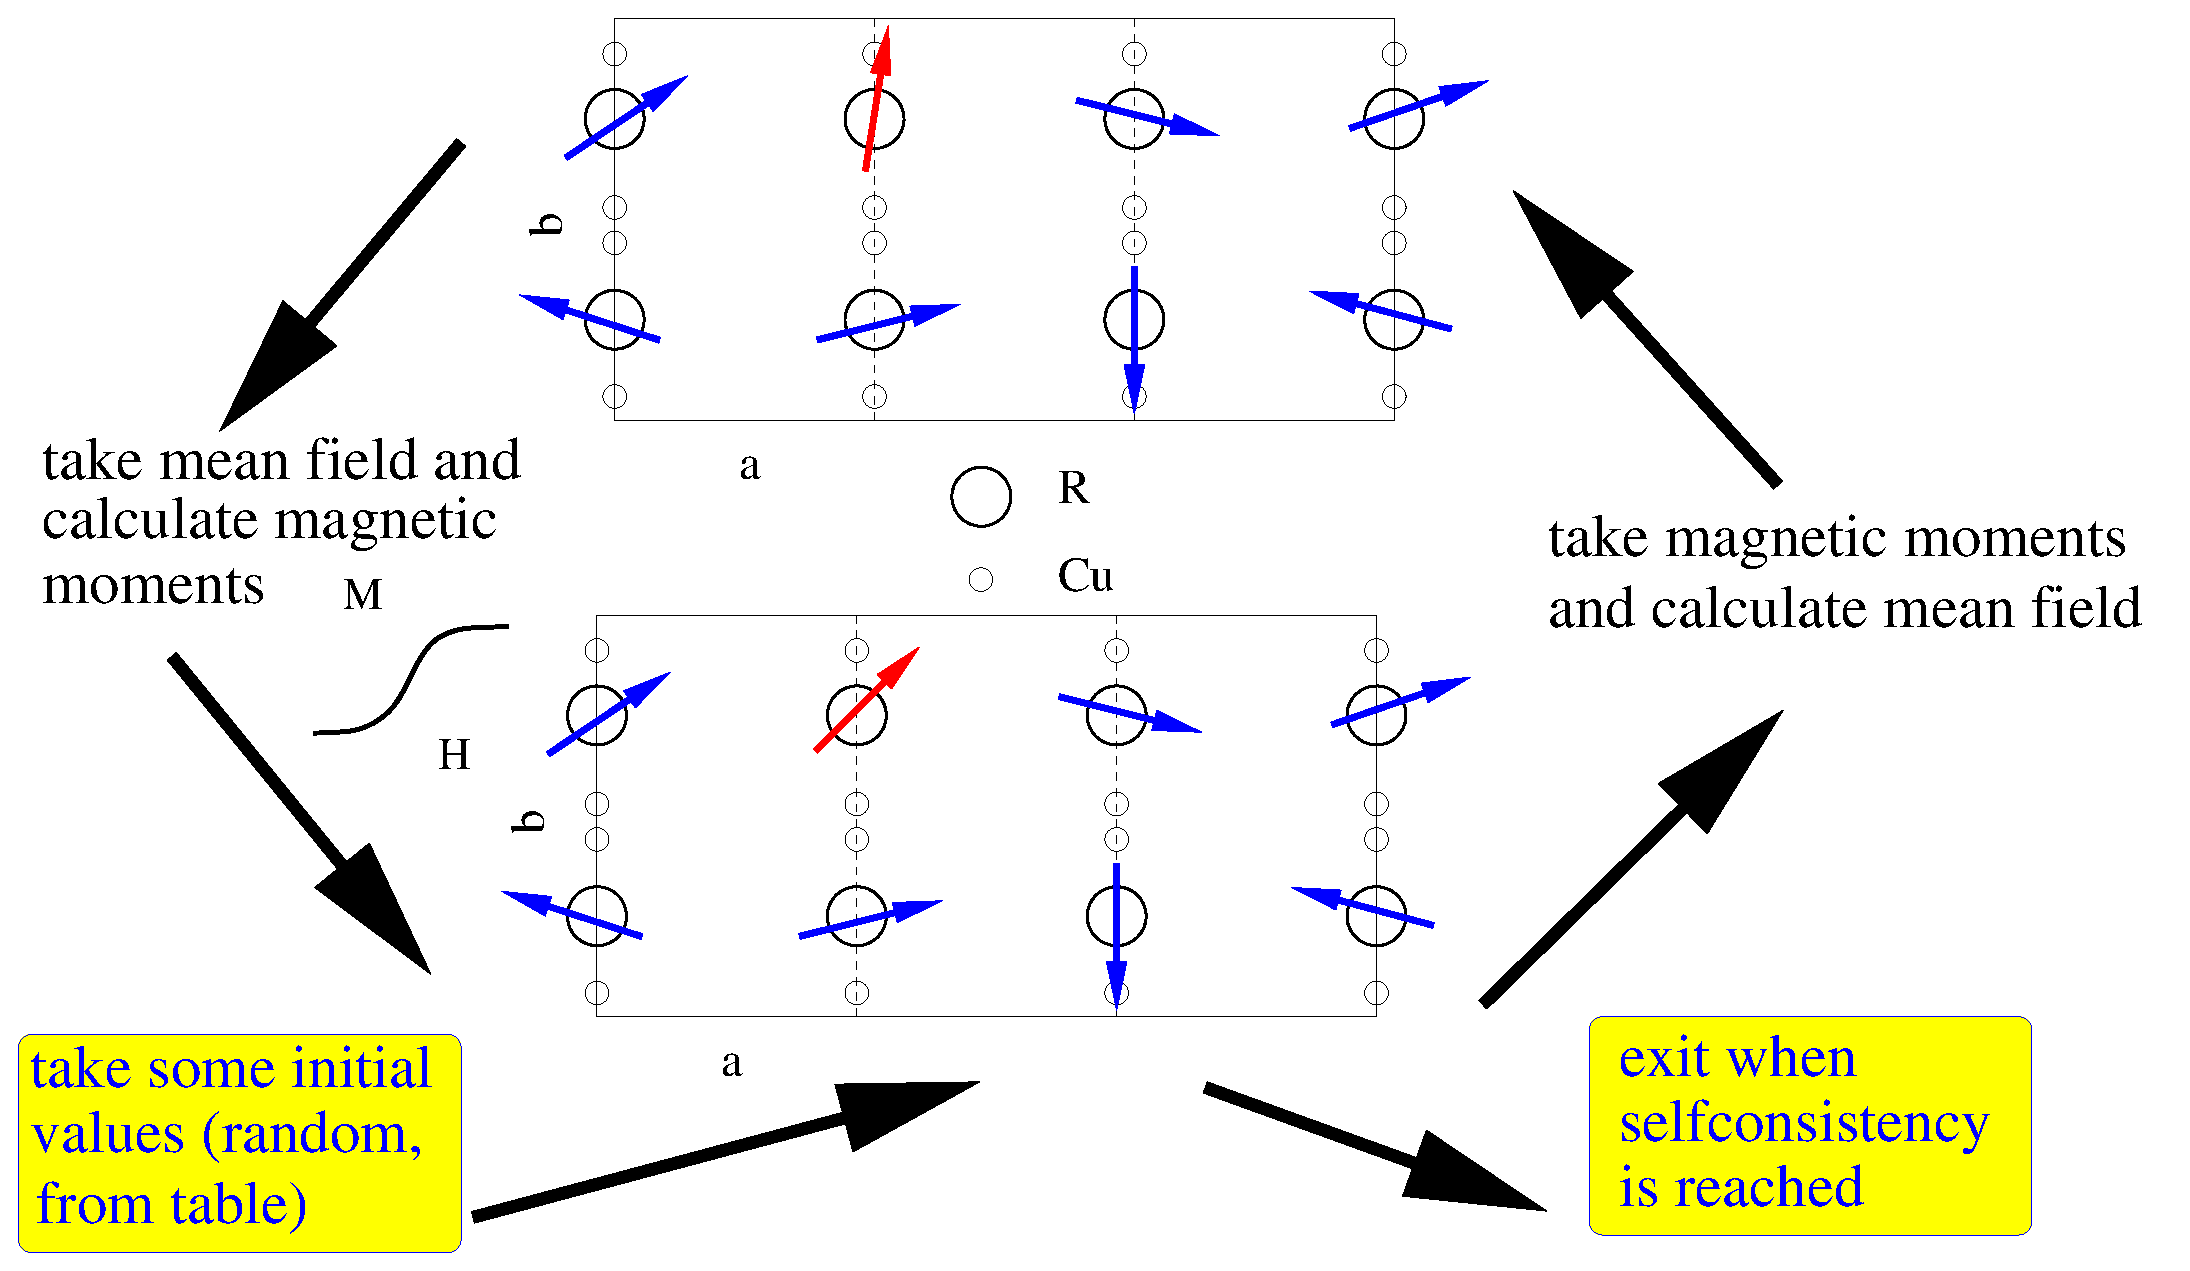
\includegraphics[angle=0,width=0.9\columnwidth]{figsrc/fecalc.eps}
\caption{\label{fecalc}Mean field process of sub {\prg fecalc}.}
\end{figure}

 
\subsubsection{Example {\prg mcphas.ini\index{mcphas.ini}} file for a simple antiferromagnet}

Here is an example of {\prg mcphas.ini\index{mcphas.ini}}, the comments describe the meaning of the different
parameters:

\input{mcphas.ini}



\subsubsection{{\prg mcphas.j\index{mcphas.j}} - lattice and exchange parameters}\label{mcphasj}
This file provides the information about 
the crystallographic
 structure and the magnetic exchange interactions.
For every atom in the crystallographic basis there
has to be given the coordinates, the number of neighbours to be considered, the 
Land\'e factor $g_J$, the single ion property filename and  a set of exchange parameters.
If the exchange parameters (and neighbour positions) are not known for your system, you 
can use the program module {\prg makenn\index{makenn}} (see section \ref{addprog}) to generate 
a list of nearest neighbours and
exchange parameters, currently implemented in {\prg makenn\index{makenn}} are dipolar interactions,
exchange interactions via the Bethe-Slater curve or the RKKY model. Note that in order
to use {\prg makenn\index{makenn}} you have to set up a working {\prg mcphas.j\index{mcphas.j}} file, which may or
may not contain neighbours and interactions.

Use program {\prg addj\index{addj}} to add exchange parameter set stored in different 
such {\prg .j} files (see section~\ref{addprog}).



\begin{description}
\item [Line 1,2:] Comment Lines
\item [Line 3:] lattice constants a,b,c and crystal angles alpha, beta, gamma 
\item [Line 4-6:] primitive lattice vectors
\item [Line 7:] Number of atoms in the primitive crystallographic unit cell ({\prg nofatoms})
\item [Line 8:] a comment line with stars
\item [Line 9:] coordinates  ($d_a$,$d_b$,$d_c$) of 1$^{st}$ magnetic ion in the crystallographic unit cell  with
respect to the lattice vectors $\vec a$,$\vec b$,$\vec c$. The number of neighbours of this 
ion, for which interaction constants are given in the interaction table (nofneighbours). 
If {\prg diagonalexchange}
is set to 0 the 9 components of the exchange tensor are given in column 4-12. 
If {\prg diagonalexchange}
 is 1, only 3 components are given (column 4-6).
If {\prg diagonalexchange}
 is 2, specific components of the exchange tensor can be given in columns 4 onwards. The indices of these components
 must be given in the following line (Line 9a below).
The Land\'e factor of the ion (gJ) and the file name of the corresponding single ion
parameter file (cffilename).
\item [Line 9a:]  If {\prg diagonalexchange=2}, then this line gives the indices of the exchange tensor corresponding to 
 the columns 4 onwards. It must have a variable called {\prg indexexchange} followed by a list of names of components of the interaction
 tensor separated by space. E.g.
 \verb|  #! indexexchange= JaJb JbJc  | 
means column 4 gives the the interaction constant between the
 first angular momentum component of the current ion with the second angular momentum component of its neighbour, whilst 
 column 5 has the interaction constant between the second angular momentum component of this ion with the third component of its
 neighbour. Alternatively, pairs of numbers may be given, as in \verb|  #! indexexchange= 1,2 2,3  |
 Additionally another parameter {\prg symmetricexchange} can be set to 1, where the value in each column is also used 
 for the transposed tensor component. Thus \verb|  #! symmetricexchange=1 indexexchange= JaJb  | is the same as \\
 \verb|  #! indexexchange= JaJb JbJa  | where the 4th and 5th column are the same.
\item [Line 10:]  Comment line
\item [Line 11-(10+nofneighbours):] Interaction table for ion number 1.   
Note: the neighbour coordinates (column 1-3) are given with respect to the lattice vectors
$\vec a$,$\vec b$,$\vec c$. The program then calculates from these values the coordinates
with respect to the primitive lattice $\vec r_1$,~$\vec r_2$,~$\vec r_3$.
($ d_a \vec a + d_b \vec b + d_c \vec c = d_1 \vec r_1 + d_2 \vec r_2 + d_3 \vec r_3$).
Column 4,5,6 \dots contain the components of the interaction tensor $\stackrel{=}{\mathcal J}$. 
Note that in case of non-orthogonal axes the 
components of the moments and the interaction tensor $Ja, Jb, Jc, Jaa, Jbb, Jcc, Jab ...$ 
refer to the orthogonal coordinate system
defined with respect to the nonorthogonal lattice $\vec a,\vec b,\vec c$ as
$Jb||\vec b$, $Jc||(\vec a \times \vec b)$ and $Ja$ perpendicular to $Jb$ and $Jc$.
\item [Line (11+nofneighbours) - end:] for each ion in the unit cell line 8 - (10+nofneighbours)
are repeated.
\end{description}


\vspace{0.5cm}

{\small {\bf Information for experienced users:}
\begin{description}
\item[\prg mcphas.jjj:]
format of exchange parameter file, which only needs a reduced set of exchange
parameters in the input file. Using the program {\prg jjj2j} the file can be transformed
to {\prg mcphas.j\index{mcphas.j}} by adding lines for all the equivalent neighbours. The format definition
of {\prg mcphas.jjj} is the same as {\prg mcphas.j\index{mcphas.j}}, however each line denotes several
equivalent neighbour atoms (instead of only one in {\prg mcphas.j\index{mcphas.j}}) according to the
 following rules:
\begin{itemize}
\item If a nonzero coordinate $d_a$ (or $d_b$,$d_c$) in the interaction table
 corresponds to it's value at the nearest
 lattice point of the primitive lattice,
  additional interactions of the same size
with  neighbours with coordinate $-d_a$ (or $-d_b$,$-d_c$, respectively)
are taken into account. This
holds for each of the three coordinates $d_a$,$d_b$ and $d_c$
 resulting in a maximum
number of 8 equivalent neighbours per line in the interaction table.
\item If the value of $d_a$ (or $d_b$,$d_c$) is zero or differs
from it's value at the nearest lattice point of the primitive lattice, it is 
changed to the value at the nearest lattice point and {\bf no} interaction 
with  neighbours with coordinates $-d_a$ (or $-d_b$,$-d_c$) is
 taken into account. If such
 interaction is needed it may be given in a different line and may
have different magnitude. In this way also crystallographic lattices
with no mirror symmetry may be described.
\end{itemize}
\item[\prg mcphas.coq:]   exchange parameters etc [ in old format]...see examples for details, use {\prg coq2jjj} to 
transform {\prg mcphas.coq} to {\prg mcphas.jjj} format
\end{description}

}


\subsubsection{Example {\prg mcphas.j\index{mcphas.j}} file for a simple antiferromagnet}

Here are example files of a tetragonal antiferromagnet with nearest neighbour interactions, all
files are equivalent:

{\small
\begin{verbatim} 
# simple antiferromagnet 
#<!--mcphase.mcphas.j-->
#***************************************************************
# Lattice Constants (A)
#! a=4.3843 b=4.3843 c=2.4194 alpha=  90 beta=  90 gamma=  90
#! r1a=   1 r2a=   0 r3a=   0
#! r1b=   0 r2b=   1 r3b=   0   primitive lattice vectors [a][b][c]
#! r1c=   0 r2c=   0 r3c=   1
#! nofatoms=1  nofcomponents=3  number of atoms in primitive unit cell/number of components of each spin
# ****************************************************************************
#! da=  0 [a] db=  0 [b] dc=  0 nofneighbours=2 diagonalexchange=0 gJ=0.857143 cffilename=Ce3p.sipf
# da[a] db[b] dc[c] Jaa[meV] Jbb[meV] Jcc[meV] Jab[meV] Jba[meV] Jac[meV] Jca[meV] Jbc[meV] Jcb[meV]
+0	+0	+1	-0.1	-0.1	-0.1   0  0  0  0  0  0
+0	+0	-1	-0.1	-0.1	-0.1   0  0  0  0  0  0
#\end{verbatim}
}

Using diagonalexchange this may be shortened to

{\small
\begin{verbatim} 
# simple antiferromagnet 
#<!--mcphase.mcphas.j-->
#***************************************************************
# Lattice Constants (A)
#! a=4.3843 b=4.3843 c=2.4194 alpha=  90 beta=  90 gamma=  90
#! r1a=   1 r2a=   0 r3a=   0
#! r1b=   0 r2b=   1 r3b=   0   primitive lattice vectors [a][b][c]
#! r1c=   0 r2c=   0 r3c=   1
#! nofatoms=1  nofcomponents=3  number of atoms in primitive unit cell/number of components of each spin
# ****************************************************************************
#! da=  0 [a] db=  0 [b] dc=  0 nofneighbours=2 diagonalexchange=1 gJ=0.857143 cffilename=Ce3p.sipf
# da[a] db[b] dc[c] Jaa[meV] Jbb[meV] Jcc[meV] Jab[meV] Jba[meV] Jac[meV] Jca[meV] Jbc[meV] Jcb[meV]
+0	+0	+1	-0.1	-0.1	-0.1   
+0	+0	-1	-0.1	-0.1	-0.1   
#\end{verbatim}
}

with indexexchange option the sequence of two ion interaction parameters can be changed and
zero parameters may be omitted:

{\small
\begin{verbatim} 
# simple antiferromagnet 
#<!--mcphase.mcphas.j-->
#***************************************************************
# Lattice Constants (A)
#! a=4.3843 b=4.3843 c=2.4194 alpha=  90 beta=  90 gamma=  90
#! r1a=   1 r2a=   0 r3a=   0
#! r1b=   0 r2b=   1 r3b=   0   primitive lattice vectors [a][b][c]
#! r1c=   0 r2c=   0 r3c=   1
#! nofatoms=1  nofcomponents=3  number of atoms in primitive unit cell/number of components of each spin
# ****************************************************************************
#! da=  0 [a] db=  0 [b] dc=  0 nofneighbours=2 diagonalexchange=2 gJ=0.857143 cffilename=Ce3p.sipf
# da[a] db[b] dc[c] Jaa[meV] Jbb[meV] Jcc[meV] Jab[meV] Jba[meV] Jac[meV] Jca[meV] Jbc[meV] Jcb[meV]
#! indexexchange = JaJa JaJc JcJa JbJb JcJc
+0	+0	+1	-0.1 0 0 -0.1	-0.1  
+0	+0	-1	-0.1 0 0 -0.1	-0.1  
#\end{verbatim}
}

{\small
\begin{verbatim} 
# simple antiferromagnet 
#<!--mcphase.mcphas.j-->
#***************************************************************
# Lattice Constants (A)
#! a=4.3843 b=4.3843 c=2.4194 alpha=  90 beta=  90 gamma=  90
#! r1a=   1 r2a=   0 r3a=   0
#! r1b=   0 r2b=   1 r3b=   0   primitive lattice vectors [a][b][c]
#! r1c=   0 r2c=   0 r3c=   1
#! nofatoms=1  nofcomponents=3  number of atoms in primitive unit cell/number of components of each spin
# ****************************************************************************
#! da=  0 [a] db=  0 [b] dc=  0 nofneighbours=2 diagonalexchange=2 gJ=0.857143 cffilename=Ce3p.sipf
# da[a] db[b] dc[c] Jaa[meV] Jbb[meV] Jcc[meV] Jab[meV] Jba[meV] Jac[meV] Jca[meV] Jbc[meV] Jcb[meV]
#! indexexchange = 1,1 1,3, 3,1 2,2 3,3
+0	+0	+1	-0.1 0 0 -0.1	-0.1  
+0	+0	-1	-0.1 0 0 -0.1	-0.1  
#\end{verbatim}
}


using symmetricexchange together with indexexchange will assume that the interaction tensor is symmetic and 
only half of it may be given:

{\small
\begin{verbatim} 
# simple antiferromagnet 
#<!--mcphase.mcphas.j-->
#***************************************************************
# Lattice Constants (A)
#! a=4.3843 b=4.3843 c=2.4194 alpha=  90 beta=  90 gamma=  90
#! r1a=   1 r2a=   0 r3a=   0
#! r1b=   0 r2b=   1 r3b=   0   primitive lattice vectors [a][b][c]
#! r1c=   0 r2c=   0 r3c=   1
#! nofatoms=1  nofcomponents=3  number of atoms in primitive unit cell/number of components of each spin
# ****************************************************************************
#! da=  0 [a] db=  0 [b] dc=  0 nofneighbours=2 diagonalexchange=2 gJ=0.857143 cffilename=Ce3p.sipf
# da[a] db[b] dc[c] Jaa[meV] Jbb[meV] Jcc[meV] Jab[meV] Jba[meV] Jac[meV] Jca[meV] Jbc[meV] Jcb[meV]
#! symmetricexchange=1 indexexchange = JaJa JaJc JbJb JcJc
+0	+0	+1	-0.1 0  -0.1	-0.1  
+0	+0	-1	-0.1 0  -0.1	-0.1  
#\end{verbatim}
}


\subsubsection{Single Ion Property Input Files}\label{sifile}

In order to speed up calculations or treat special problems a large 
variety of single ion modules is available. This includes the
option to load a user written single ion module. Details are 
given in chapter~\ref{simod}.

The first time user of {\prg McPhase} should use the module {\prg so1ion}\index{so1ion} and 
create an appropriate single ion property input file as described in
section \ref{cf1ion}. A good starting point are several examples
given in directory {\prg examples}.


\subsubsection{Example single ion property file  for a simple antiferromagnet}

Here is an example file {\prg mcphas.cf1} describing the anisotropy of a 
simple antiferromagnet with Ce atoms having basal plane anisotropy. Note the
axis convention xyz$||$abc, in case of non-orthogonal axes the convention 
is $y||\vec b$, $z||(\vec a \times \vec b)$ and $x$ perpendicular to $y$ and $z$.


\input{mcphas.cf1}

\subsubsection{{\prg mcphas.tst\index{mcphas.tst}} - input file of test spin-configurations (optional)}
This file is optional and contains
some test momentum configurations to be used for the calculation
             of the free energy. Mind that
\begin{itemize}
\item  in the file header the number of atoms in the primitive
       crystallographic unit cell and the number of components
       of the spin vector have to be given.
\item  at the end of the
 file there must be no empty lines !
\end{itemize}

The momentum - configurations tables always refer to spins sitting on
the primitive lattice ${\mbf r}_i$. If more than one atom is in
the primitive basis, the momentum gets $3n$ components ($n=$ number
of atoms in the crystallographic basis). See {\prg ./examples/ndcu2b\_new/} for
examples of a two atom basis. Units of these tables are that of total 
angular momentum $<J>$.

\subsubsection{Example {\prg mcphas.tst\index{mcphas.tst}} file  for a simple antiferromagnet}

Here is the file {\prg mcphas.tst\index{mcphas.tst}} for the simple antiferromagnet example
describing some spin configurations
to be used as starting values for the mean field process:

\input{mcphas.tst}
Note, in case of non-orthogonal axes the convention 
is $mb||\vec b$, $mc||(\vec a \times \vec b)$ and $ma$ perpendicular to $mb$ and $mc$.

\subsubsection{subdirectory {\prg ./results} - directory where calculated data is stored}

In order to be able to save the results of a calculation the directory {\prg ./results} has to
exist. Mind that all files in this directory will be overwritten without warning. 

\subsubsection{subdirectory {\prg ./fit} - experimental data for fit (optional) } 

In order that {\prg McPhase} can calculate the standard deviation between
 experimental data and the results of the simulation, some experimental data
 can be given in the subdirectory {\prg ./fit}. The filenames and the data-format
 are the same as the output files of {\prg McPhas}, e.g. {\prg mcphas.fum}, {\prg mcphas.hkl}
 etc. {\prg McPhase} looks into the directory {\prg ./fit} and if it finds any
 of these files, the standard deviation is increased correspondingly. 

What measurement data can be used to calculate a standard deviation ?

\begin{description}
\item[{\prg mcphas.fum}] if given in column 11, 12, 13 in {\prg ./fit/mcphas.fum} the
            magnetisation in the $a$, $b$ and $c$ direction is used for calculation
	    of the standard deviation sta. The standard deviation is calculated
	    as ${\rm sta}=\sum_{\rm data points i} ({\mbf m}_i^{calc}-{\mbf m}_i^{meas})^2$.
	    All three components of the magnetic moment have to be given and are used.

\end{description}

Note that the measured data has to be given in those (H-T) points which are 
calculated by mcphas\index{mcphas} in order to be used by the program to increase {\prg sta}.
It is usually most effective to fit only few data points, because a large set
of data points will not improve the quality of the fit and only require a large
amount of calculation time.



\subsection{Starting a simulation}
\label{start}

To start the simulation goto the directory containing the
input files {\prg mcphas.ini, mcphas.j, etc. } and type

\begin{description}
\item[\prg mcphas] to run the program generating stepwise $H-T$ values 
              in a loop given by {\prg mcphas.ini\index{mcphas.ini}} (you can also press the
              symbol in the {\prg McPhase - Explorer} window).
\item[\prg mcphas\index{mcphas} [file]]  to run the program with an input file --   
             {\prg file} contains T ha hb hc values to be calculated 
             if [file] is not given, xmin xmax xstep (xT xHa xHb xHc)
             ymin ymax ystep (yT yHa yHb yHc) is read from file {\prg mcphas.ini\index{mcphas.ini}}
	     and phase diagram is calculated
\item[\prg mcphas\index{mcphas} -h]  to  print help and version of {\prg McPhas}.
\item[\prg mcphas\index{mcphas} -stamax 14]  end mcphas\index{mcphas} if standard deviation exceeds 14.
\item[\prg mcphas\index{mcphas} -a] avoid overwriting output files in results, append new results to existing files
\item[\prg mcphas\index{mcphas} -v]  to  enable verbose mode with lots of messages of {\prg McPhas}. Specifically
the verbose mode enables the following features:
  \begin{itemize}
			          \item more information is printed out, 
			          \item the q-vectors file {\prg ./results/mcphas.qvc} will contain 
				    the explicit spin configurations
			          \item the display\index{display} on screen (ghostview window using 
				     {\prg ./results/.sps.eps}) will be updated not only 
				    when a H-T point has been finished but always 
				    when a structure with smaller free energy 
				    has been stabilised
  \end{itemize}
\item[\prg mcphasit\index{mcphas}] to start mcphase in commandline mode without opening any window
\end{description}

\vspace{1cm}
{\em Exercises:}
\begin{itemize}
\item Look at the input files for {\prg McPhase} given in the directory
{\prg examples/ndcu2b\_new}.  How many atoms are contained in the crystallographic basis ?
\item
Start the simulation by typing the command {\prg mcphas}.
\end{itemize}



\subsection{Options for a running simulation}
... when the program is running, the options in the main window
can be changed. Pressing ''displayall'' displays the current spin-configuration
at each iteration step. Pressing ''log fe vs Q'' appends free energy vs Q
data to {\prg mcphas.log} for every ($T-H$) point.


The file {\prg ./results/.spins.eps} is used to show the information about the currently calculated
spin structure on the screen using the postscript file viewer ghostview.

The file {\prg ./results/.mcphas.fum} contains the information of the magnetisation curve
which is currently calculated. This information is automatically displayed on the screen.


The program {\prg display} (see section \ref{display}) can be used 
for the online display\index{display} of any other
curve(s).


\subsection{Output Files - {\prg mcphas.qvc,phs,sps,mf,fum,j1...,xyt,hkl} }\label{outputfiles}
 (in directory ./results/ after a simulation run) 

\begin{figure}[htb]%h=here, t=top, b=bottom, p=separate figure page
\begin{center}\leavevmode
\includegraphics[angle=0, width=0.3\textwidth]{figsrc/magnetization_ndcu2.ps}
\end{center}
\caption{Calculated magnetisation of NdCu$_2$ for field parallel to the orthorhombic $b$-direction.}
\label{magnetization}
\end{figure}

\begin{figure}[htb]%h=here, t=top, b=bottom, p=separate figure page
\begin{center}\leavevmode
\includegraphics[angle=0, width=0.8\textwidth]{figsrc/magnetostriction_ndcu2.eps}
\end{center}
\caption{Calculated spontaneous magnetostriction of NdCu$_2$.}
\label{magnetostrictiongraphic}
\end{figure}

\begin{description}
\item [\prg mcphas.qvc]    the set of test q-vectors used for calculation of free energy.
                           Components of these q vectors refer to the reciprocal lattice $\vec a^*,\vec b^*,\vec c^*$.
\item [\prg mcphas.phs]    spin-configuration table of different types of spin-configurations. 
                            Note, in case of non-orthogonal axes the convention in these tables 
                            is $mb||\vec b$, $mc||(\vec a \times \vec b)$ and $ma$ perpendicular to $mb$ and $mc$.

                           {\em Note}: 
                           there is no natural criteria for deciding, if one spin-configuration is
			   different from another one. Therefore the list of ''different''
			   spin-configurations is dependent on the meaning of ''different''.
			   
			   The program {\prg McPhase} decides whether a spin-configuration is
			   different from another by a simple criteria, namely by the
			   angle between the spins. Comparing two spin configurations it calculates
			   the angle between corresponding spins and if for one spin the
			   angle is not small, the configuration is treated as a different
			   configuration. Therefore for example a ferromagnet with moments
			   in $a$ has a different spin configuration than a ferromagnet with
			   moments in $b$ direction. 
\item [\prg mcphas.sps]    $T-H$ dependence of spin-configuration. The spin configurations stored in this
                           file may be displayed using the program {\prg spins\index{spins}}, an example is given
			   in figure~\ref{spingraphic}.
                            Note, in case of non-orthogonal axes the convention for applied field $Ha, Hb,Hc$ and
                            also for the moment components $ma, mb, mc$ in these tables 
                            is $mb||\vec b$, $mc||(\vec a \times \vec b)$ and $ma$ perpendicular to $mb$ and $mc$.

\item [\prg mcphas.mf]     $T-H$ dependence of exchange field configuration, stored as $g_J \mu_B H_{xc}(i)$(unit is in meV)
                            for i=1,2,...,number of spins in magnetic unit cell.
                            Note, in case of non-orthogonal axes the convention for applied field $Ha, Hb,Hc$ and
                            also for the mean field components in these tables 
                            is $Hb||\vec b$, $Hc||(\vec a \times \vec b)$ and $Ha$ perpendicular to $Hb$ and $Hc$.
\item [\prg mcphas.fum]    free energy, magnetic energy (the derivative with respect to temperature gives the specific %%@
heat),
                           magnetisation data and (if cfield is used with higher order interactions)
                           expectation values of the Stevens Operators $<O_l^m>$ . As an example for the information
			   contained in this file the calculated magnetisation and magnetostriction of NdCu$_2$ is shown in
			   figures~\ref{magnetization} and ~\ref{magnetizationgraphic}.
                            Note, in case of non-orthogonal axes the convention for applied field $Ha, Hb,Hc$ and
                            also for the magnetisation components $ma,mb,mc$ in these tables 
                            is $Hb||\vec b$, $Hc||(\vec a \times \vec b)$ and $Ha$ perpendicular to $Hb$ and $Hc$.

\item [\prg mcphas1.j1 .j1 .j2 ...] 
               spin-spin correlation functions for sub-lattice 1 neighbour 1 2 ...
	       (linear combination is proportional to magnetostriction)
	       The spin-spin correlation functions for neighbour $k$ are defined by
	       the following sum of dyadic products:

	       \begin{equation}
	        \frac{1}{n}\sum_{s=1}^n <{\mbf J}^s> \times  <{\mbf J}^{s+k}>
	       \end{equation}
	       with $n$ being the number of moments in the magnetic unit cell.
	       Single ion and two-ion magnetostriction can be calculated using the $<O_l^m>$ and the
	       spin-spin correlation functions. As an example the magnetostriction analysis of
	       NdCu$_2$ is shown in figure~\ref{magnetostrictiongraphic}. For details 
             please refer to~\cite{rotter02-8885}.
                            Note, in case of non-orthogonal axes the convention for applied field $Ha, Hb,Hc$ and
                            also for the moment components in these tables 
                            is $Hb||\vec b$, $Hc||(\vec a \times \vec b)$ and $Ha$ perpendicular to $Hb$ and $Hc$.
\item [\prg mcphas.xyt]    phase diagram as x,y,T, H, phase-number j according to spin-configuration table
               given in mcphas.phs, a periodicity key, nettomoments <J>.
 Figure~\ref{phasediagramgraphic}
	       shows the phase diagram of NdCu$_2$ for magnetic fields parallel to the orthorhombic $b$-direction.
                            Note, in case of non-orthogonal axes the convention for applied field $Ha, Hb,Hc$ 
                             in these tables 
                            is $Hb||\vec b$, $Hc||(\vec a \times \vec b)$ and $Ha$ perpendicular to $Hb$ and $Hc$.
\item [\prg mcphas.hkl]    calculated (unpolarised) neutron diffraction data (the calculated magnetic intensities
    correspond to the magnetic structure + Polarisation factor. The
    Lorentz-factor , magnetic form factor and  instrumental corrections are not calculated.)
 As an example figure~\ref{neutintgraphic}
    shows the calculated temperature dependence of magnetic amplitudes for NdCu$_2$.
                           $h,k,l$ refer to the reciprocal lattice $\vec a^*,\vec b^*,\vec c^*$.
                            Note, in case of non-orthogonal axes the convention for applied field $Ha, Hb,Hc$ 
                             in these tables 
                            is $Hb||\vec b$, $Hc||(\vec a \times \vec b)$ and $Ha$ perpendicular to $Hb$ and $Hc$.
    
\item [\prg mcphasa.hkl]    Fourier Transform of the $a$-component of the magnetic Moments.
                           $h,k,l$ refer to the reciprocal lattice $\vec a^*,\vec b^*,\vec c^*$.
                            Note, in case of non-orthogonal axes the convention for applied field $Ha, Hb,Hc$ and
                            the magnetic moment component in these tables 
                            is $Hb||\vec b$, $Hc||(\vec a \times \vec b)$ and $Ha$ perpendicular to $Hb$ and $Hc$.
\item [\prg mcphasb.hkl]    Fourier Transform of the $b$-component of the magnetic Moments.
                           $h,k,l$ refer to the reciprocal lattice $\vec a^*,\vec b^*,\vec c^*$.
                            Note, in case of non-orthogonal axes the convention for applied field $Ha, Hb,Hc$ and
                            the magnetic moment component in these tables 
                            is $Hb||\vec b$, $Hc||(\vec a \times \vec b)$ and $Ha$ perpendicular to $Hb$ and $Hc$.
\item [\prg mcphasc.hkl]    Fourier Transform of the $c$-component of the magnetic Moments.
                           $h,k,l$ refer to the reciprocal lattice $\vec a^*,\vec b^*,\vec c^*$.
                            Note, in case of non-orthogonal axes the convention for applied field $Ha, Hb,Hc$ and
                            the magnetic moment component in these tables 
                            is $Hb||\vec b$, $Hc||(\vec a \times \vec b)$ and $Ha$ perpendicular to $Hb$ and $Hc$.
\end{description} 

\vspace{1cm}
{\em Exercises:}
\begin{itemize}
\item Look at the output files of {\prg McPhase}  in the directory
{\prg examples/ndcu2b\_new/results}.  At which magnetic field
the ferromagnetically aligned state is achieved (at $T=$2~K)?
\item
What is the propagation vector in the different antiferromagnetic phases at $T=$2~K ?
\end{itemize}


Note, in case of non-orthogonal axes the convention 
is $mb||\vec b$, $mc||(\vec a \times \vec b)$ and $ma$ perpendicular to $mb$ and $mc$.

\subsubsection{subdirectory {\prg ./results} - directory where calculated data is stored}

In order to be able to save the results of a calculation the directory {\prg ./results} has to
exist. Mind that all files in this directory will be overwritten without warning. 

\subsubsection{subdirectory {\prg ./fit} - experimental data for fit (optional) } 

In order that {\prg McPhase} can calculate the standard deviation between
 experimental data and the results of the simulation, some experimental data
 can be given in the subdirectory {\prg ./fit}. The filenames and the data-format
 are the same as the output files of {\prg McPhas}, e.g. {\prg mcphas.fum}, {\prg mcphas.hkl}
 etc. {\prg McPhase} looks into the directory {\prg ./fit} and if it finds any
 of these files, the standard deviation is increased correspondingly. 

What measurement data can be used to calculate a standard deviation ?

\begin{description}
\item[{\prg mcphas.fum}] if given in column 11, 12, 13 in {\prg ./fit/mcphas.fum} the
            magnetisation in the $a$, $b$ and $c$ direction is used for calculation
	    of the standard deviation sta. The standard deviation is calculated
	    as ${\rm sta}=\sum_{\rm data points i} ({\mbf m}_i^{calc}-{\mbf m}_i^{meas})^2$.
	    All three components of the magnetic moment have to be given and are used.

\end{description}

Note that the measured data has to be given in those (H-T) points which are 
calculated by mcphas\index{mcphas} in order to be used by the program to increase {\prg sta}.
It is usually most effective to fit only few data points, because a large set
of data points will not improve the quality of the fit and only require a large
amount of calculation time.



\subsection{Starting a simulation}
\label{start}

To start the simulation goto the directory containing the
input files {\prg mcphas.ini, mcphas.j, etc. } and type

\begin{description}
\item[\prg mcphas] to run the program generating stepwise $H-T$ values 
              in a loop given by {\prg mcphas.ini\index{mcphas.ini}} (you can also press the
              symbol in the {\prg McPhase - Explorer} window).
\item[\prg mcphas\index{mcphas} [file]]  to run the program with an input file --   
             {\prg file} contains T ha hb hc values to be calculated 
             if [file] is not given, xmin xmax xstep (xT xHa xHb xHc)
             ymin ymax ystep (yT yHa yHb yHc) is read from file {\prg mcphas.ini\index{mcphas.ini}}
	     and phase diagram is calculated
\item[\prg mcphas\index{mcphas} -h]  to  print help and version of {\prg McPhas}.
\item[\prg mcphas\index{mcphas} -stamax 14]  end mcphas\index{mcphas} if standard deviation exceeds 14.
\item[\prg mcphas\index{mcphas} -a] avoid overwriting output files in results, append new results to existing files
\item[\prg mcphas\index{mcphas} -v]  to  enable verbose mode with lots of messages of {\prg McPhas}. Specifically
the verbose mode enables the following features:
  \begin{itemize}
			          \item more information is printed out, 
			          \item the q-vectors file {\prg ./results/mcphas.qvc} will contain 
				    the explicit spin configurations
			          \item the display\index{display} on screen (ghostview window using 
				     {\prg ./results/.sps.eps}) will be updated not only 
				    when a H-T point has been finished but always 
				    when a structure with smaller free energy 
				    has been stabilised
  \end{itemize}
\item[\prg mcphasit\index{mcphas}] to start mcphase in commandline mode without opening any window
\end{description}

\vspace{1cm}
{\em Exercises:}
\begin{itemize}
\item Look at the input files for {\prg McPhase} given in the directory
{\prg examples/ndcu2b\_new}.  How many atoms are contained in the crystallographic basis ?
\item
Start the simulation by typing the command {\prg mcphas}.
\end{itemize}



\subsection{Options for a running simulation}
... when the program is running, the options in the main window
can be changed. Pressing ''displayall'' displays the current spin-configuration
at each iteration step. Pressing ''log fe vs Q'' appends free energy vs Q
data to {\prg mcphas.log} for every ($T-H$) point.


The file {\prg ./results/.spins.eps} is used to show the information about the currently calculated
spin structure on the screen using the postscript file viewer ghostview.

The file {\prg ./results/.mcphas.fum} contains the information of the magnetisation curve
which is currently calculated. This information is automatically displayed on the screen.


The program {\prg display} (see section \ref{display}) can be used 
for the online display\index{display} of any other
curve(s).


\subsection{Output Files - {\prg mcphas.qvc,phs,sps,mf,fum,j1...,xyt,hkl} }\label{outputfiles}
 (in directory ./results/ after a simulation run) 

\begin{figure}[htb]%h=here, t=top, b=bottom, p=separate figure page
\begin{center}\leavevmode
\includegraphics[angle=0, width=0.3\textwidth]{figsrc/magnetization_ndcu2.ps}
\end{center}
\caption{Calculated magnetisation of NdCu$_2$ for field parallel to the orthorhombic $b$-direction.}
\label{magnetization}
\end{figure}

\begin{figure}[htb]%h=here, t=top, b=bottom, p=separate figure page
\begin{center}\leavevmode
\includegraphics[angle=0, width=0.8\textwidth]{figsrc/magnetostriction_ndcu2.eps}
\end{center}
\caption{Calculated spontaneous magnetostriction of NdCu$_2$.}
\label{magnetostrictiongraphic}
\end{figure}

\begin{description}
\item [\prg mcphas.qvc]    the set of test q-vectors used for calculation of free energy.
                           Components of these q vectors refer to the reciprocal lattice $\vec a^*,\vec b^*,\vec c^*$.
\item [\prg mcphas.phs]    spin-configuration table of different types of spin-configurations. 
                            Note, in case of non-orthogonal axes the convention in these tables 
                            is $mb||\vec b$, $mc||(\vec a \times \vec b)$ and $ma$ perpendicular to $mb$ and $mc$.

                           {\em Note}: 
                           there is no natural criteria for deciding, if one spin-configuration is
			   different from another one. Therefore the list of ''different''
			   spin-configurations is dependent on the meaning of ''different''.
			   
			   The program {\prg McPhase} decides whether a spin-configuration is
			   different from another by a simple criteria, namely by the
			   angle between the spins. Comparing two spin configurations it calculates
			   the angle between corresponding spins and if for one spin the
			   angle is not small, the configuration is treated as a different
			   configuration. Therefore for example a ferromagnet with moments
			   in $a$ has a different spin configuration than a ferromagnet with
			   moments in $b$ direction. 
\item [\prg mcphas.sps]    $T-H$ dependence of spin-configuration. The spin configurations stored in this
                           file may be displayed using the program {\prg spins\index{spins}}, an example is given
			   in figure~\ref{spingraphic}.
                            Note, in case of non-orthogonal axes the convention for applied field $Ha, Hb,Hc$ and
                            also for the moment components $ma, mb, mc$ in these tables 
                            is $mb||\vec b$, $mc||(\vec a \times \vec b)$ and $ma$ perpendicular to $mb$ and $mc$.

\item [\prg mcphas.mf]     $T-H$ dependence of exchange field configuration, stored as $g_J \mu_B H_{xc}(i)$(unit is in meV)
                            for i=1,2,...,number of spins in magnetic unit cell.
                            Note, in case of non-orthogonal axes the convention for applied field $Ha, Hb,Hc$ and
                            also for the mean field components in these tables 
                            is $Hb||\vec b$, $Hc||(\vec a \times \vec b)$ and $Ha$ perpendicular to $Hb$ and $Hc$.
\item [\prg mcphas.fum]    free energy, magnetic energy (the derivative with respect to temperature gives the specific %%@
heat),
                           magnetisation data and (if cfield is used with higher order interactions)
                           expectation values of the Stevens Operators $<O_l^m>$ . As an example for the information
			   contained in this file the calculated magnetisation and magnetostriction of NdCu$_2$ is shown in
			   figures~\ref{magnetization} and ~\ref{magnetizationgraphic}.
                            Note, in case of non-orthogonal axes the convention for applied field $Ha, Hb,Hc$ and
                            also for the magnetisation components $ma,mb,mc$ in these tables 
                            is $Hb||\vec b$, $Hc||(\vec a \times \vec b)$ and $Ha$ perpendicular to $Hb$ and $Hc$.

\item [\prg mcphas1.j1 .j1 .j2 ...] 
               spin-spin correlation functions for sub-lattice 1 neighbour 1 2 ...
	       (linear combination is proportional to magnetostriction)
	       The spin-spin correlation functions for neighbour $k$ are defined by
	       the following sum of dyadic products:

	       \begin{equation}
	        \frac{1}{n}\sum_{s=1}^n <{\mbf J}^s> \times  <{\mbf J}^{s+k}>
	       \end{equation}
	       with $n$ being the number of moments in the magnetic unit cell.
	       Single ion and two-ion magnetostriction can be calculated using the $<O_l^m>$ and the
	       spin-spin correlation functions. As an example the magnetostriction analysis of
	       NdCu$_2$ is shown in figure~\ref{magnetostrictiongraphic}. For details 
             please refer to~\cite{rotter02-8885}.
                            Note, in case of non-orthogonal axes the convention for applied field $Ha, Hb,Hc$ and
                            also for the moment components in these tables 
                            is $Hb||\vec b$, $Hc||(\vec a \times \vec b)$ and $Ha$ perpendicular to $Hb$ and $Hc$.
\item [\prg mcphas.xyt]    phase diagram as x,y,T, H, phase-number j according to spin-configuration table
               given in mcphas.phs, a periodicity key, nettomoments <J>.
 Figure~\ref{phasediagramgraphic}
	       shows the phase diagram of NdCu$_2$ for magnetic fields parallel to the orthorhombic $b$-direction.
                            Note, in case of non-orthogonal axes the convention for applied field $Ha, Hb,Hc$ 
                             in these tables 
                            is $Hb||\vec b$, $Hc||(\vec a \times \vec b)$ and $Ha$ perpendicular to $Hb$ and $Hc$.
\item [\prg mcphas.hkl]    calculated (unpolarised) neutron diffraction data (the calculated magnetic intensities
    correspond to the magnetic structure + Polarisation factor. The
    Lorentz-factor , magnetic form factor and  instrumental corrections are not calculated.)
 As an example figure~\ref{neutintgraphic}
    shows the calculated temperature dependence of magnetic amplitudes for NdCu$_2$.
                           $h,k,l$ refer to the reciprocal lattice $\vec a^*,\vec b^*,\vec c^*$.
                            Note, in case of non-orthogonal axes the convention for applied field $Ha, Hb,Hc$ 
                             in these tables 
                            is $Hb||\vec b$, $Hc||(\vec a \times \vec b)$ and $Ha$ perpendicular to $Hb$ and $Hc$.
    
\item [\prg mcphasa.hkl]    Fourier Transform of the $a$-component of the magnetic Moments.
                           $h,k,l$ refer to the reciprocal lattice $\vec a^*,\vec b^*,\vec c^*$.
                            Note, in case of non-orthogonal axes the convention for applied field $Ha, Hb,Hc$ and
                            the magnetic moment component in these tables 
                            is $Hb||\vec b$, $Hc||(\vec a \times \vec b)$ and $Ha$ perpendicular to $Hb$ and $Hc$.
\item [\prg mcphasb.hkl]    Fourier Transform of the $b$-component of the magnetic Moments.
                           $h,k,l$ refer to the reciprocal lattice $\vec a^*,\vec b^*,\vec c^*$.
                            Note, in case of non-orthogonal axes the convention for applied field $Ha, Hb,Hc$ and
                            the magnetic moment component in these tables 
                            is $Hb||\vec b$, $Hc||(\vec a \times \vec b)$ and $Ha$ perpendicular to $Hb$ and $Hc$.
\item [\prg mcphasc.hkl]    Fourier Transform of the $c$-component of the magnetic Moments.
                           $h,k,l$ refer to the reciprocal lattice $\vec a^*,\vec b^*,\vec c^*$.
                            Note, in case of non-orthogonal axes the convention for applied field $Ha, Hb,Hc$ and
                            the magnetic moment component in these tables 
                            is $Hb||\vec b$, $Hc||(\vec a \times \vec b)$ and $Ha$ perpendicular to $Hb$ and $Hc$.
\end{description} 

\vspace{1cm}
{\em Exercises:}
\begin{itemize}
\item Look at the output files of {\prg McPhase}  in the directory
{\prg examples/ndcu2b\_new/results}.  At which magnetic field
the ferromagnetically aligned state is achieved (at $T=$2~K)?
\item
What is the propagation vector in the different antiferromagnetic phases at $T=$2~K ?
\end{itemize}





\subsubsection{{\prg mcphas.j\index{mcphas.j}} - lattice and exchange parameters}\label{mcphasj}
This file provides the information about 
the crystallographic
 structure and the magnetic exchange interactions.
For every atom in the crystallographic basis there
has to be given the coordinates, the number of neighbours to be considered, the 
Land\'e factor $g_J$, the single ion property filename and  a set of exchange parameters.
If the exchange parameters (and neighbour positions) are not known for your system, you 
can use the program module {\prg makenn\index{makenn}} (see section \ref{addprog}) to generate 
a list of nearest neighbours and
exchange parameters, currently implemented in {\prg makenn\index{makenn}} are dipolar interactions,
exchange interactions via the Bethe-Slater curve or the RKKY model. Note that in order
to use {\prg makenn\index{makenn}} you have to set up a working {\prg mcphas.j\index{mcphas.j}} file, which may or
may not contain neighbours and interactions.

Use program {\prg addj\index{addj}} to add exchange parameter set stored in different 
such {\prg .j} files (see section~\ref{addprog}).



\begin{description}
\item [Line 1,2:] Comment Lines
\item [Line 3:] lattice constants a,b,c and crystal angles alpha, beta, gamma 
\item [Line 4-6:] primitive lattice vectors
\item [Line 7:] Number of atoms in the primitive crystallographic unit cell ({\prg nofatoms})
\item [Line 8:] a comment line with stars
\item [Line 9:] coordinates  ($d_a$,$d_b$,$d_c$) of 1$^{st}$ magnetic ion in the crystallographic unit cell  with
respect to the lattice vectors $\vec a$,$\vec b$,$\vec c$. The number of neighbours of this 
ion, for which interaction constants are given in the interaction table (nofneighbours). 
If {\prg diagonalexchange}
is set to 0 the 9 components of the exchange tensor are given in column 4-12. 
If {\prg diagonalexchange}
 is 1, only 3 components are given (column 4-6).
If {\prg diagonalexchange}
 is 2, specific components of the exchange tensor can be given in columns 4 onwards. The indices of these components
 must be given in the following line (Line 9a below).
The Land\'e factor of the ion (gJ) and the file name of the corresponding single ion
parameter file (cffilename).
\item [Line 9a:]  If {\prg diagonalexchange=2}, then this line gives the indices of the exchange tensor corresponding to 
 the columns 4 onwards. It must have a variable called {\prg indexexchange} followed by a list of names of components of the interaction
 tensor separated by space. E.g.
 \verb|  #! indexexchange= JaJb JbJc  | 
means column 4 gives the the interaction constant between the
 first angular momentum component of the current ion with the second angular momentum component of its neighbour, whilst 
 column 5 has the interaction constant between the second angular momentum component of this ion with the third component of its
 neighbour. Alternatively, pairs of numbers may be given, as in \verb|  #! indexexchange= 1,2 2,3  |
 Additionally another parameter {\prg symmetricexchange} can be set to 1, where the value in each column is also used 
 for the transposed tensor component. Thus \verb|  #! symmetricexchange=1 indexexchange= JaJb  | is the same as \\
 \verb|  #! indexexchange= JaJb JbJa  | where the 4th and 5th column are the same.
\item [Line 10:]  Comment line
\item [Line 11-(10+nofneighbours):] Interaction table for ion number 1.   
Note: the neighbour coordinates (column 1-3) are given with respect to the lattice vectors
$\vec a$,$\vec b$,$\vec c$. The program then calculates from these values the coordinates
with respect to the primitive lattice $\vec r_1$,~$\vec r_2$,~$\vec r_3$.
($ d_a \vec a + d_b \vec b + d_c \vec c = d_1 \vec r_1 + d_2 \vec r_2 + d_3 \vec r_3$).
Column 4,5,6 \dots contain the components of the interaction tensor $\stackrel{=}{\mathcal J}$. 
Note that in case of non-orthogonal axes the 
components of the moments and the interaction tensor $Ja, Jb, Jc, Jaa, Jbb, Jcc, Jab ...$ 
refer to the orthogonal coordinate system
defined with respect to the nonorthogonal lattice $\vec a,\vec b,\vec c$ as
$Jb||\vec b$, $Jc||(\vec a \times \vec b)$ and $Ja$ perpendicular to $Jb$ and $Jc$.
\item [Line (11+nofneighbours) - end:] for each ion in the unit cell line 8 - (10+nofneighbours)
are repeated.
\end{description}


\vspace{0.5cm}

{\small {\bf Information for experienced users:}
\begin{description}
\item[\prg mcphas.jjj:]
format of exchange parameter file, which only needs a reduced set of exchange
parameters in the input file. Using the program {\prg jjj2j} the file can be transformed
to {\prg mcphas.j\index{mcphas.j}} by adding lines for all the equivalent neighbours. The format definition
of {\prg mcphas.jjj} is the same as {\prg mcphas.j\index{mcphas.j}}, however each line denotes several
equivalent neighbour atoms (instead of only one in {\prg mcphas.j\index{mcphas.j}}) according to the
 following rules:
\begin{itemize}
\item If a nonzero coordinate $d_a$ (or $d_b$,$d_c$) in the interaction table
 corresponds to it's value at the nearest
 lattice point of the primitive lattice,
  additional interactions of the same size
with  neighbours with coordinate $-d_a$ (or $-d_b$,$-d_c$, respectively)
are taken into account. This
holds for each of the three coordinates $d_a$,$d_b$ and $d_c$
 resulting in a maximum
number of 8 equivalent neighbours per line in the interaction table.
\item If the value of $d_a$ (or $d_b$,$d_c$) is zero or differs
from it's value at the nearest lattice point of the primitive lattice, it is 
changed to the value at the nearest lattice point and {\bf no} interaction 
with  neighbours with coordinates $-d_a$ (or $-d_b$,$-d_c$) is
 taken into account. If such
 interaction is needed it may be given in a different line and may
have different magnitude. In this way also crystallographic lattices
with no mirror symmetry may be described.
\end{itemize}
\item[\prg mcphas.coq:]   exchange parameters etc [ in old format]...see examples for details, use {\prg coq2jjj} to 
transform {\prg mcphas.coq} to {\prg mcphas.jjj} format
\end{description}

}


\subsubsection{Example {\prg mcphas.j\index{mcphas.j}} file for a simple antiferromagnet}

Here are example files of a tetragonal antiferromagnet with nearest neighbour interactions, all
files are equivalent:

{\small
\begin{verbatim} 
# simple antiferromagnet 
#<!--mcphase.mcphas.j-->
#***************************************************************
# Lattice Constants (A)
#! a=4.3843 b=4.3843 c=2.4194 alpha=  90 beta=  90 gamma=  90
#! r1a=   1 r2a=   0 r3a=   0
#! r1b=   0 r2b=   1 r3b=   0   primitive lattice vectors [a][b][c]
#! r1c=   0 r2c=   0 r3c=   1
#! nofatoms=1  nofcomponents=3  number of atoms in primitive unit cell/number of components of each spin
# ****************************************************************************
#! da=  0 [a] db=  0 [b] dc=  0 nofneighbours=2 diagonalexchange=0 gJ=0.857143 cffilename=Ce3p.sipf
# da[a] db[b] dc[c] Jaa[meV] Jbb[meV] Jcc[meV] Jab[meV] Jba[meV] Jac[meV] Jca[meV] Jbc[meV] Jcb[meV]
+0	+0	+1	-0.1	-0.1	-0.1   0  0  0  0  0  0
+0	+0	-1	-0.1	-0.1	-0.1   0  0  0  0  0  0
#\end{verbatim}
}

Using diagonalexchange this may be shortened to

{\small
\begin{verbatim} 
# simple antiferromagnet 
#<!--mcphase.mcphas.j-->
#***************************************************************
# Lattice Constants (A)
#! a=4.3843 b=4.3843 c=2.4194 alpha=  90 beta=  90 gamma=  90
#! r1a=   1 r2a=   0 r3a=   0
#! r1b=   0 r2b=   1 r3b=   0   primitive lattice vectors [a][b][c]
#! r1c=   0 r2c=   0 r3c=   1
#! nofatoms=1  nofcomponents=3  number of atoms in primitive unit cell/number of components of each spin
# ****************************************************************************
#! da=  0 [a] db=  0 [b] dc=  0 nofneighbours=2 diagonalexchange=1 gJ=0.857143 cffilename=Ce3p.sipf
# da[a] db[b] dc[c] Jaa[meV] Jbb[meV] Jcc[meV] Jab[meV] Jba[meV] Jac[meV] Jca[meV] Jbc[meV] Jcb[meV]
+0	+0	+1	-0.1	-0.1	-0.1   
+0	+0	-1	-0.1	-0.1	-0.1   
#\end{verbatim}
}

with indexexchange option the sequence of two ion interaction parameters can be changed and
zero parameters may be omitted:

{\small
\begin{verbatim} 
# simple antiferromagnet 
#<!--mcphase.mcphas.j-->
#***************************************************************
# Lattice Constants (A)
#! a=4.3843 b=4.3843 c=2.4194 alpha=  90 beta=  90 gamma=  90
#! r1a=   1 r2a=   0 r3a=   0
#! r1b=   0 r2b=   1 r3b=   0   primitive lattice vectors [a][b][c]
#! r1c=   0 r2c=   0 r3c=   1
#! nofatoms=1  nofcomponents=3  number of atoms in primitive unit cell/number of components of each spin
# ****************************************************************************
#! da=  0 [a] db=  0 [b] dc=  0 nofneighbours=2 diagonalexchange=2 gJ=0.857143 cffilename=Ce3p.sipf
# da[a] db[b] dc[c] Jaa[meV] Jbb[meV] Jcc[meV] Jab[meV] Jba[meV] Jac[meV] Jca[meV] Jbc[meV] Jcb[meV]
#! indexexchange = JaJa JaJc JcJa JbJb JcJc
+0	+0	+1	-0.1 0 0 -0.1	-0.1  
+0	+0	-1	-0.1 0 0 -0.1	-0.1  
#\end{verbatim}
}

{\small
\begin{verbatim} 
# simple antiferromagnet 
#<!--mcphase.mcphas.j-->
#***************************************************************
# Lattice Constants (A)
#! a=4.3843 b=4.3843 c=2.4194 alpha=  90 beta=  90 gamma=  90
#! r1a=   1 r2a=   0 r3a=   0
#! r1b=   0 r2b=   1 r3b=   0   primitive lattice vectors [a][b][c]
#! r1c=   0 r2c=   0 r3c=   1
#! nofatoms=1  nofcomponents=3  number of atoms in primitive unit cell/number of components of each spin
# ****************************************************************************
#! da=  0 [a] db=  0 [b] dc=  0 nofneighbours=2 diagonalexchange=2 gJ=0.857143 cffilename=Ce3p.sipf
# da[a] db[b] dc[c] Jaa[meV] Jbb[meV] Jcc[meV] Jab[meV] Jba[meV] Jac[meV] Jca[meV] Jbc[meV] Jcb[meV]
#! indexexchange = 1,1 1,3, 3,1 2,2 3,3
+0	+0	+1	-0.1 0 0 -0.1	-0.1  
+0	+0	-1	-0.1 0 0 -0.1	-0.1  
#\end{verbatim}
}


using symmetricexchange together with indexexchange will assume that the interaction tensor is symmetic and 
only half of it may be given:

{\small
\begin{verbatim} 
# simple antiferromagnet 
#<!--mcphase.mcphas.j-->
#***************************************************************
# Lattice Constants (A)
#! a=4.3843 b=4.3843 c=2.4194 alpha=  90 beta=  90 gamma=  90
#! r1a=   1 r2a=   0 r3a=   0
#! r1b=   0 r2b=   1 r3b=   0   primitive lattice vectors [a][b][c]
#! r1c=   0 r2c=   0 r3c=   1
#! nofatoms=1  nofcomponents=3  number of atoms in primitive unit cell/number of components of each spin
# ****************************************************************************
#! da=  0 [a] db=  0 [b] dc=  0 nofneighbours=2 diagonalexchange=2 gJ=0.857143 cffilename=Ce3p.sipf
# da[a] db[b] dc[c] Jaa[meV] Jbb[meV] Jcc[meV] Jab[meV] Jba[meV] Jac[meV] Jca[meV] Jbc[meV] Jcb[meV]
#! symmetricexchange=1 indexexchange = JaJa JaJc JbJb JcJc
+0	+0	+1	-0.1 0  -0.1	-0.1  
+0	+0	-1	-0.1 0  -0.1	-0.1  
#\end{verbatim}
}


\subsubsection{Single Ion Property Input Files}\label{sifile}

In order to speed up calculations or treat special problems a large 
variety of single ion modules is available. This includes the
option to load a user written single ion module. Details are 
given in chapter~\ref{simod}.

The first time user of {\prg McPhase} should use the module {\prg so1ion}\index{so1ion} and 
create an appropriate single ion property input file as described in
section \ref{cf1ion}. A good starting point are several examples
given in directory {\prg examples}.


\subsubsection{Example single ion property file  for a simple antiferromagnet}

Here is an example file {\prg mcphas.cf1} describing the anisotropy of a 
simple antiferromagnet with Ce atoms having basal plane anisotropy. Note the
axis convention xyz$||$abc, in case of non-orthogonal axes the convention 
is $y||\vec b$, $z||(\vec a \times \vec b)$ and $x$ perpendicular to $y$ and $z$.


\section{{\prg mcphas} - calculation of thermodynamic properties (Magnetisation, Susceptibility, Specific Heat, Neutron %%@
Diffraction, etc.)}
\label{runmcphas}

In order to perform calculations beyond the capabilities of {\prg cfield\index{cfield}} it is necessary
to use the program {\prg mcphas}. 
\begin{itemize}
\item As a first step it is possible to
calculate the thermodynamic properties such as magnetisation or specific heat
considering only single ion effects. In this case all the exchange parameters
have to be set to zero in {\prg mcphas.j\index{mcphas.j}}. 
\item for more advanced calculations the two - ion interactions have to be
considered and may lead to magnetic order. {\prg mcphas} can perform 
calculations in the ordered state in the following way: for 
a given temperature $T$ and magnetic field $\mbf H$ (vector)
several possible magnetic structures are stabilised
by a mean field algorithm and the free energy is 
calculated. The initial values for this mean-field procedure are
modified by a Monte Carlo process.


The temperature and magnetic field is varied during the calculation
and thereby it is possible to map out the magnetic phase diagram.
\end{itemize}

The program produces a plot of the stabilised magnetic
structures and the magnetisation on screen, the
output files contain additional information 
such as calculated magnetoelastic and  neutron-scattering
data. Several graphic programs easy the visualisation of the
calculated data (section~\ref{graphics}).



\subsection{Input Files}
The program {\prg McPhase} needs the following input files (all in the same directory)
 in order to run:

\begin{enumerate}
\item {\prg mcphas.ini\index{mcphas.ini}}
 - controlling the algorithm
\item {\prg mcphas.j\index{mcphas.j}}
  - lattice and exchange parameters
\item {\prg mcphas.tst\index{mcphas.tst}(optional)}  - test spin configurations
\item {\prg single-ion property files}
\item {\prg directory ./results/}
 - directory where calculated data is stored
\item {\prg directory ./fit} - experimental data for fit (optional)
\end{enumerate}


 All
 of these input files have to be in one directory and the program
has to be started in this directory. The results of the simulation
are then stored in the  subdirectory ./results/, which must exist before starting
the program 
... see directory ./examples/ for some examples.
 In order to prepare these files
for a new calculation it is best to take them from an example, copy the files
to a new directory and make the
modifications  to adapt them to the new problem.

\subsubsection{Example - a simple antiferromagnet}

In the following description of the input files we will always refer
to a simple example: a simple antiferromagnet
on a primitive orthorhombic lattice. The first time user
will thus have a simple example to follow, all corresponding
files are given in the directory {\prg tutorial/03magnetic\_phases\_mcphas/simpleAF}.
 

\subsubsection{{\prg mcphas.ini\index{mcphas.ini}} - controlling the algorithm}
   Initial file containing algorithm control parameters, for instance the range and spacing of
   propagation vectors Q or the number of Monte Carlo trials for initial spin configurations
    - {\em mind}: this
   file is rewritten and reread  when running the program and may be changed by the
   user in order to manipulate the running simulation.

{\prg mcphas.ini\index{mcphas.ini}} consists of several sections:
\begin{description}
\item [MCPHASE RUNTIME CONTROL:] this section contains the parameters
controlling the status of the calculation.
\item [XY PHASEDIAGRAM PARAMETERS:] here the temperature and field range and
step widths of the calculation are specified.
The definition of the x and y
axis in terms of temperature and magnetic field is followed by the
corresponding range and step width. An offset may be given for all
field and temperature values.
Note that for most cases of interest
this offset is zero (T0=0, Ha0=0, Hb0=0, Hc0=0).
 For the simple case of calculating a Temperature-Field phase diagram
 It is just necessary to set xT=1 and give the temperature range by
xmin/xmax/xstep. For field in b direction then just set yHb=1 and 
define the range in ymin/ymax/ystep.
In case of non-orthogonal axes the applied magnetic field
components $Ha, Hb, Hc$ refer to the orthogonal coordinate system
defined with respect to the nonorthogonal lattice $\mbf a,\mbf b,\mbf c$ as
$Hb||\mbf b$, $Hc||(\mbf a \times \mbf b)$ and $Ha$ perpendicular to $Hb$ and $Hc$.

\item [GENERATION OF SPINCONFIGURATIONS:] at the beginning of the program
some initial values of spin configurations are generated from a set of 
propagation vectors. This section defines the range of propagation vectors
and the step width.
Depending on the value of the propagation Q with respect to the primitive reciprocal lattice
1-, 2- or 3-dimensional simulations of magnetic lattices
are possible. It is advisable to 
think carefully about the chosen range and spacing of Q vectors in order
to limit calculation time.
 
For example a good starting point is to begin with a calculation with large
step widths (e.g. 0.1)  covering the Brillouin zone. This should give an idea
of the propagation vectors which are stabilised. An advanced calculation
could then fine tune the propagation and determine its accurate value (using
small step widths in a limited area of the zone).
The verbose option of {\prg mcphas} allows to inspect the propagation vectors
which are actually used in the calculation.
Trick: in order to get a quick overview of the
q-vector range covered by the mcphas\index{mcphas} simulation start mcphas, exit and 
just type {\prg felog ./results/mcphas.qvc} (need {\prg perl,perldl,pdl,pgplot} packages).

In order to limit calculation time, the maximum periodicity
of the magnetic unit cell with respect to the crystallographic unit cell 
(maxqperiod) and the maximum number of spins in the magnetic unit cell 
(maxnofspins) can be limited. Also the maximum number of test spin configurations
in the internal table can be limited (maxnoftestspincf).
A critical feature with respect to calculation time is also the number of
spin configurations which are generated by a random process from a tabulated
SPINCONFIGURATIONS during the calculation. 

In summary the variables in this section are mainly important to adapt the
program to a given computer system with finite speed. They have to be set
to optimise between speed and accuracy of the calculation. In order to
find appropriate values it is best to perform some calculations 
and restrict the parameters step by step if insufficient speed is obtained.
Also the examples included in the program package may serve as starting
points.

\item [PARAMETERS FOR SUB FECALC SELFCONSISTENCY PROCESS:] the most important
procedure in the module {\prg mcphas} is the sub fecalc. In this part of the 
program the self consistent calculation of the magnetic moment configuration
is performed as shown schematically in fig.~\ref{fecalc}. 
In the mean field approximation the Hamiltonian~(\ref{hamilton}) is approximated
by

\begin{equation}
 {\mathcal H}=\sum_n H_{SI}^n + E_{corr}
\end{equation}

with the single ion Hamiltonian (in case of module {\prg so1ion\index{so1ion}})

\begin{equation}
H_{SI}^n=  B_l^m O_{lm}({\mbf J}^n) 
	     - g_{Jn} \mu_B {\mbf J}^n {\mbf H^n_{eff}} 
\end{equation}

and the correction term

\begin{equation}
E_{corr}=\frac{1}{2}\sum_{n} g_{Jn} \mu_B \langle {\mbf J}^n
 \rangle (\mbf H^n_{eff}-\mbf H) 
\end{equation}

and with the mean fields $ \mbf H^n_{eff}$ given by

\begin{equation}\label{meanfield}
\mbf H^n_{eff}=\mbf H + \mbf H^n_{xc}=\mbf H+\sum_{{\mbf G'}n'} \frac{{\mathcal J}
(\mbf r_n-(\mbf G'+\mbf r_{n'}))}{g_{Jn}\mu_B } \langle{\mbf
J}^{n'}\rangle
\end{equation}

These mean fields and the moments $\langle \mbf J^n \rangle$ 
are determined in a self consistent
way. For a given magnetic unit cell and initial configuration 
of magnetic moments
the mean fields are calculated according to equation~(\ref{meanfield}). 
Then, for each
magnetic ion the single ion property module is taken 
and the magnetic moment $\langle \mbf J^n \rangle$ is 
calculated from it's mean field. The mean fields are used again in equation~(\ref{meanfield})
and so on .... until convergence is reached. 
Then, the free energy ($f=-kT\sum_n \ln(z_n) + E_{corr}$ ) 
of the stabilised
configuration is calculated (this is why this sub is called {\prg fecalc}). 
The free energies of a lot of different stabilised configurations have to
be compared in order to find out which configuration has lowest free energy, i.e.
is stable in thermal  equilibrium.

It may happen that this process does
not converge due to bad choice of the initial configuration, therefore a maximum number
of mean field loops has to be given by the user.
The results of a calculation may be significantly influenced by
changing parameters such as the maximum number of iteration loops 
in this section. 
In fact the simulation is always a compromise of calculation time and accuracy: if only
a few initial spin configurations are tried at each (H-T) point, the calculation speed is
fast, however it is possible that the program misses the magnetic structure with the
lowest free energy. The same holds if other critical parameters of the simulation are
restricted too much.
 

\item [OUTPUT OF PHYSICAL PROPERTIES:]
Some options for the output of the calculation can be changed in this section.
\end{description}

\begin{figure}[hb]
\includegraphics[angle=0,width=0.9\columnwidth]{figsrc/fecalc.eps}
\caption{\label{fecalc}Mean field process of sub {\prg fecalc}.}
\end{figure}

 
\subsubsection{Example {\prg mcphas.ini\index{mcphas.ini}} file for a simple antiferromagnet}

Here is an example of {\prg mcphas.ini\index{mcphas.ini}}, the comments describe the meaning of the different
parameters:

\section{{\prg mcphas} - calculation of thermodynamic properties (Magnetisation, Susceptibility, Specific Heat, Neutron %%@
Diffraction, etc.)}
\label{runmcphas}

In order to perform calculations beyond the capabilities of {\prg cfield\index{cfield}} it is necessary
to use the program {\prg mcphas}. 
\begin{itemize}
\item As a first step it is possible to
calculate the thermodynamic properties such as magnetisation or specific heat
considering only single ion effects. In this case all the exchange parameters
have to be set to zero in {\prg mcphas.j\index{mcphas.j}}. 
\item for more advanced calculations the two - ion interactions have to be
considered and may lead to magnetic order. {\prg mcphas} can perform 
calculations in the ordered state in the following way: for 
a given temperature $T$ and magnetic field $\mbf H$ (vector)
several possible magnetic structures are stabilised
by a mean field algorithm and the free energy is 
calculated. The initial values for this mean-field procedure are
modified by a Monte Carlo process.


The temperature and magnetic field is varied during the calculation
and thereby it is possible to map out the magnetic phase diagram.
\end{itemize}

The program produces a plot of the stabilised magnetic
structures and the magnetisation on screen, the
output files contain additional information 
such as calculated magnetoelastic and  neutron-scattering
data. Several graphic programs easy the visualisation of the
calculated data (section~\ref{graphics}).



\subsection{Input Files}
The program {\prg McPhase} needs the following input files (all in the same directory)
 in order to run:

\begin{enumerate}
\item {\prg mcphas.ini\index{mcphas.ini}}
 - controlling the algorithm
\item {\prg mcphas.j\index{mcphas.j}}
  - lattice and exchange parameters
\item {\prg mcphas.tst\index{mcphas.tst}(optional)}  - test spin configurations
\item {\prg single-ion property files}
\item {\prg directory ./results/}
 - directory where calculated data is stored
\item {\prg directory ./fit} - experimental data for fit (optional)
\end{enumerate}


 All
 of these input files have to be in one directory and the program
has to be started in this directory. The results of the simulation
are then stored in the  subdirectory ./results/, which must exist before starting
the program 
... see directory ./examples/ for some examples.
 In order to prepare these files
for a new calculation it is best to take them from an example, copy the files
to a new directory and make the
modifications  to adapt them to the new problem.

\subsubsection{Example - a simple antiferromagnet}

In the following description of the input files we will always refer
to a simple example: a simple antiferromagnet
on a primitive orthorhombic lattice. The first time user
will thus have a simple example to follow, all corresponding
files are given in the directory {\prg tutorial/03magnetic\_phases\_mcphas/simpleAF}.
 

\subsubsection{{\prg mcphas.ini\index{mcphas.ini}} - controlling the algorithm}
   Initial file containing algorithm control parameters, for instance the range and spacing of
   propagation vectors Q or the number of Monte Carlo trials for initial spin configurations
    - {\em mind}: this
   file is rewritten and reread  when running the program and may be changed by the
   user in order to manipulate the running simulation.

{\prg mcphas.ini\index{mcphas.ini}} consists of several sections:
\begin{description}
\item [MCPHASE RUNTIME CONTROL:] this section contains the parameters
controlling the status of the calculation.
\item [XY PHASEDIAGRAM PARAMETERS:] here the temperature and field range and
step widths of the calculation are specified.
The definition of the x and y
axis in terms of temperature and magnetic field is followed by the
corresponding range and step width. An offset may be given for all
field and temperature values.
Note that for most cases of interest
this offset is zero (T0=0, Ha0=0, Hb0=0, Hc0=0).
 For the simple case of calculating a Temperature-Field phase diagram
 It is just necessary to set xT=1 and give the temperature range by
xmin/xmax/xstep. For field in b direction then just set yHb=1 and 
define the range in ymin/ymax/ystep.
In case of non-orthogonal axes the applied magnetic field
components $Ha, Hb, Hc$ refer to the orthogonal coordinate system
defined with respect to the nonorthogonal lattice $\mbf a,\mbf b,\mbf c$ as
$Hb||\mbf b$, $Hc||(\mbf a \times \mbf b)$ and $Ha$ perpendicular to $Hb$ and $Hc$.

\item [GENERATION OF SPINCONFIGURATIONS:] at the beginning of the program
some initial values of spin configurations are generated from a set of 
propagation vectors. This section defines the range of propagation vectors
and the step width.
Depending on the value of the propagation Q with respect to the primitive reciprocal lattice
1-, 2- or 3-dimensional simulations of magnetic lattices
are possible. It is advisable to 
think carefully about the chosen range and spacing of Q vectors in order
to limit calculation time.
 
For example a good starting point is to begin with a calculation with large
step widths (e.g. 0.1)  covering the Brillouin zone. This should give an idea
of the propagation vectors which are stabilised. An advanced calculation
could then fine tune the propagation and determine its accurate value (using
small step widths in a limited area of the zone).
The verbose option of {\prg mcphas} allows to inspect the propagation vectors
which are actually used in the calculation.
Trick: in order to get a quick overview of the
q-vector range covered by the mcphas\index{mcphas} simulation start mcphas, exit and 
just type {\prg felog ./results/mcphas.qvc} (need {\prg perl,perldl,pdl,pgplot} packages).

In order to limit calculation time, the maximum periodicity
of the magnetic unit cell with respect to the crystallographic unit cell 
(maxqperiod) and the maximum number of spins in the magnetic unit cell 
(maxnofspins) can be limited. Also the maximum number of test spin configurations
in the internal table can be limited (maxnoftestspincf).
A critical feature with respect to calculation time is also the number of
spin configurations which are generated by a random process from a tabulated
SPINCONFIGURATIONS during the calculation. 

In summary the variables in this section are mainly important to adapt the
program to a given computer system with finite speed. They have to be set
to optimise between speed and accuracy of the calculation. In order to
find appropriate values it is best to perform some calculations 
and restrict the parameters step by step if insufficient speed is obtained.
Also the examples included in the program package may serve as starting
points.

\item [PARAMETERS FOR SUB FECALC SELFCONSISTENCY PROCESS:] the most important
procedure in the module {\prg mcphas} is the sub fecalc. In this part of the 
program the self consistent calculation of the magnetic moment configuration
is performed as shown schematically in fig.~\ref{fecalc}. 
In the mean field approximation the Hamiltonian~(\ref{hamilton}) is approximated
by

\begin{equation}
 {\mathcal H}=\sum_n H_{SI}^n + E_{corr}
\end{equation}

with the single ion Hamiltonian (in case of module {\prg so1ion\index{so1ion}})

\begin{equation}
H_{SI}^n=  B_l^m O_{lm}({\mbf J}^n) 
	     - g_{Jn} \mu_B {\mbf J}^n {\mbf H^n_{eff}} 
\end{equation}

and the correction term

\begin{equation}
E_{corr}=\frac{1}{2}\sum_{n} g_{Jn} \mu_B \langle {\mbf J}^n
 \rangle (\mbf H^n_{eff}-\mbf H) 
\end{equation}

and with the mean fields $ \mbf H^n_{eff}$ given by

\begin{equation}\label{meanfield}
\mbf H^n_{eff}=\mbf H + \mbf H^n_{xc}=\mbf H+\sum_{{\mbf G'}n'} \frac{{\mathcal J}
(\mbf r_n-(\mbf G'+\mbf r_{n'}))}{g_{Jn}\mu_B } \langle{\mbf
J}^{n'}\rangle
\end{equation}

These mean fields and the moments $\langle \mbf J^n \rangle$ 
are determined in a self consistent
way. For a given magnetic unit cell and initial configuration 
of magnetic moments
the mean fields are calculated according to equation~(\ref{meanfield}). 
Then, for each
magnetic ion the single ion property module is taken 
and the magnetic moment $\langle \mbf J^n \rangle$ is 
calculated from it's mean field. The mean fields are used again in equation~(\ref{meanfield})
and so on .... until convergence is reached. 
Then, the free energy ($f=-kT\sum_n \ln(z_n) + E_{corr}$ ) 
of the stabilised
configuration is calculated (this is why this sub is called {\prg fecalc}). 
The free energies of a lot of different stabilised configurations have to
be compared in order to find out which configuration has lowest free energy, i.e.
is stable in thermal  equilibrium.

It may happen that this process does
not converge due to bad choice of the initial configuration, therefore a maximum number
of mean field loops has to be given by the user.
The results of a calculation may be significantly influenced by
changing parameters such as the maximum number of iteration loops 
in this section. 
In fact the simulation is always a compromise of calculation time and accuracy: if only
a few initial spin configurations are tried at each (H-T) point, the calculation speed is
fast, however it is possible that the program misses the magnetic structure with the
lowest free energy. The same holds if other critical parameters of the simulation are
restricted too much.
 

\item [OUTPUT OF PHYSICAL PROPERTIES:]
Some options for the output of the calculation can be changed in this section.
\end{description}

\begin{figure}[hb]
\includegraphics[angle=0,width=0.9\columnwidth]{figsrc/fecalc.eps}
\caption{\label{fecalc}Mean field process of sub {\prg fecalc}.}
\end{figure}

 
\subsubsection{Example {\prg mcphas.ini\index{mcphas.ini}} file for a simple antiferromagnet}

Here is an example of {\prg mcphas.ini\index{mcphas.ini}}, the comments describe the meaning of the different
parameters:

\input{mcphas.ini}



\subsubsection{{\prg mcphas.j\index{mcphas.j}} - lattice and exchange parameters}\label{mcphasj}
This file provides the information about 
the crystallographic
 structure and the magnetic exchange interactions.
For every atom in the crystallographic basis there
has to be given the coordinates, the number of neighbours to be considered, the 
Land\'e factor $g_J$, the single ion property filename and  a set of exchange parameters.
If the exchange parameters (and neighbour positions) are not known for your system, you 
can use the program module {\prg makenn\index{makenn}} (see section \ref{addprog}) to generate 
a list of nearest neighbours and
exchange parameters, currently implemented in {\prg makenn\index{makenn}} are dipolar interactions,
exchange interactions via the Bethe-Slater curve or the RKKY model. Note that in order
to use {\prg makenn\index{makenn}} you have to set up a working {\prg mcphas.j\index{mcphas.j}} file, which may or
may not contain neighbours and interactions.

Use program {\prg addj\index{addj}} to add exchange parameter set stored in different 
such {\prg .j} files (see section~\ref{addprog}).



\begin{description}
\item [Line 1,2:] Comment Lines
\item [Line 3:] lattice constants a,b,c and crystal angles alpha, beta, gamma 
\item [Line 4-6:] primitive lattice vectors
\item [Line 7:] Number of atoms in the primitive crystallographic unit cell ({\prg nofatoms})
\item [Line 8:] a comment line with stars
\item [Line 9:] coordinates  ($d_a$,$d_b$,$d_c$) of 1$^{st}$ magnetic ion in the crystallographic unit cell  with
respect to the lattice vectors $\vec a$,$\vec b$,$\vec c$. The number of neighbours of this 
ion, for which interaction constants are given in the interaction table (nofneighbours). 
If {\prg diagonalexchange}
is set to 0 the 9 components of the exchange tensor are given in column 4-12. 
If {\prg diagonalexchange}
 is 1, only 3 components are given (column 4-6).
If {\prg diagonalexchange}
 is 2, specific components of the exchange tensor can be given in columns 4 onwards. The indices of these components
 must be given in the following line (Line 9a below).
The Land\'e factor of the ion (gJ) and the file name of the corresponding single ion
parameter file (cffilename).
\item [Line 9a:]  If {\prg diagonalexchange=2}, then this line gives the indices of the exchange tensor corresponding to 
 the columns 4 onwards. It must have a variable called {\prg indexexchange} followed by a list of names of components of the interaction
 tensor separated by space. E.g.
 \verb|  #! indexexchange= JaJb JbJc  | 
means column 4 gives the the interaction constant between the
 first angular momentum component of the current ion with the second angular momentum component of its neighbour, whilst 
 column 5 has the interaction constant between the second angular momentum component of this ion with the third component of its
 neighbour. Alternatively, pairs of numbers may be given, as in \verb|  #! indexexchange= 1,2 2,3  |
 Additionally another parameter {\prg symmetricexchange} can be set to 1, where the value in each column is also used 
 for the transposed tensor component. Thus \verb|  #! symmetricexchange=1 indexexchange= JaJb  | is the same as \\
 \verb|  #! indexexchange= JaJb JbJa  | where the 4th and 5th column are the same.
\item [Line 10:]  Comment line
\item [Line 11-(10+nofneighbours):] Interaction table for ion number 1.   
Note: the neighbour coordinates (column 1-3) are given with respect to the lattice vectors
$\vec a$,$\vec b$,$\vec c$. The program then calculates from these values the coordinates
with respect to the primitive lattice $\vec r_1$,~$\vec r_2$,~$\vec r_3$.
($ d_a \vec a + d_b \vec b + d_c \vec c = d_1 \vec r_1 + d_2 \vec r_2 + d_3 \vec r_3$).
Column 4,5,6 \dots contain the components of the interaction tensor $\stackrel{=}{\mathcal J}$. 
Note that in case of non-orthogonal axes the 
components of the moments and the interaction tensor $Ja, Jb, Jc, Jaa, Jbb, Jcc, Jab ...$ 
refer to the orthogonal coordinate system
defined with respect to the nonorthogonal lattice $\vec a,\vec b,\vec c$ as
$Jb||\vec b$, $Jc||(\vec a \times \vec b)$ and $Ja$ perpendicular to $Jb$ and $Jc$.
\item [Line (11+nofneighbours) - end:] for each ion in the unit cell line 8 - (10+nofneighbours)
are repeated.
\end{description}


\vspace{0.5cm}

{\small {\bf Information for experienced users:}
\begin{description}
\item[\prg mcphas.jjj:]
format of exchange parameter file, which only needs a reduced set of exchange
parameters in the input file. Using the program {\prg jjj2j} the file can be transformed
to {\prg mcphas.j\index{mcphas.j}} by adding lines for all the equivalent neighbours. The format definition
of {\prg mcphas.jjj} is the same as {\prg mcphas.j\index{mcphas.j}}, however each line denotes several
equivalent neighbour atoms (instead of only one in {\prg mcphas.j\index{mcphas.j}}) according to the
 following rules:
\begin{itemize}
\item If a nonzero coordinate $d_a$ (or $d_b$,$d_c$) in the interaction table
 corresponds to it's value at the nearest
 lattice point of the primitive lattice,
  additional interactions of the same size
with  neighbours with coordinate $-d_a$ (or $-d_b$,$-d_c$, respectively)
are taken into account. This
holds for each of the three coordinates $d_a$,$d_b$ and $d_c$
 resulting in a maximum
number of 8 equivalent neighbours per line in the interaction table.
\item If the value of $d_a$ (or $d_b$,$d_c$) is zero or differs
from it's value at the nearest lattice point of the primitive lattice, it is 
changed to the value at the nearest lattice point and {\bf no} interaction 
with  neighbours with coordinates $-d_a$ (or $-d_b$,$-d_c$) is
 taken into account. If such
 interaction is needed it may be given in a different line and may
have different magnitude. In this way also crystallographic lattices
with no mirror symmetry may be described.
\end{itemize}
\item[\prg mcphas.coq:]   exchange parameters etc [ in old format]...see examples for details, use {\prg coq2jjj} to 
transform {\prg mcphas.coq} to {\prg mcphas.jjj} format
\end{description}

}


\subsubsection{Example {\prg mcphas.j\index{mcphas.j}} file for a simple antiferromagnet}

Here are example files of a tetragonal antiferromagnet with nearest neighbour interactions, all
files are equivalent:

{\small
\begin{verbatim} 
# simple antiferromagnet 
#<!--mcphase.mcphas.j-->
#***************************************************************
# Lattice Constants (A)
#! a=4.3843 b=4.3843 c=2.4194 alpha=  90 beta=  90 gamma=  90
#! r1a=   1 r2a=   0 r3a=   0
#! r1b=   0 r2b=   1 r3b=   0   primitive lattice vectors [a][b][c]
#! r1c=   0 r2c=   0 r3c=   1
#! nofatoms=1  nofcomponents=3  number of atoms in primitive unit cell/number of components of each spin
# ****************************************************************************
#! da=  0 [a] db=  0 [b] dc=  0 nofneighbours=2 diagonalexchange=0 gJ=0.857143 cffilename=Ce3p.sipf
# da[a] db[b] dc[c] Jaa[meV] Jbb[meV] Jcc[meV] Jab[meV] Jba[meV] Jac[meV] Jca[meV] Jbc[meV] Jcb[meV]
+0	+0	+1	-0.1	-0.1	-0.1   0  0  0  0  0  0
+0	+0	-1	-0.1	-0.1	-0.1   0  0  0  0  0  0
#\end{verbatim}
}

Using diagonalexchange this may be shortened to

{\small
\begin{verbatim} 
# simple antiferromagnet 
#<!--mcphase.mcphas.j-->
#***************************************************************
# Lattice Constants (A)
#! a=4.3843 b=4.3843 c=2.4194 alpha=  90 beta=  90 gamma=  90
#! r1a=   1 r2a=   0 r3a=   0
#! r1b=   0 r2b=   1 r3b=   0   primitive lattice vectors [a][b][c]
#! r1c=   0 r2c=   0 r3c=   1
#! nofatoms=1  nofcomponents=3  number of atoms in primitive unit cell/number of components of each spin
# ****************************************************************************
#! da=  0 [a] db=  0 [b] dc=  0 nofneighbours=2 diagonalexchange=1 gJ=0.857143 cffilename=Ce3p.sipf
# da[a] db[b] dc[c] Jaa[meV] Jbb[meV] Jcc[meV] Jab[meV] Jba[meV] Jac[meV] Jca[meV] Jbc[meV] Jcb[meV]
+0	+0	+1	-0.1	-0.1	-0.1   
+0	+0	-1	-0.1	-0.1	-0.1   
#\end{verbatim}
}

with indexexchange option the sequence of two ion interaction parameters can be changed and
zero parameters may be omitted:

{\small
\begin{verbatim} 
# simple antiferromagnet 
#<!--mcphase.mcphas.j-->
#***************************************************************
# Lattice Constants (A)
#! a=4.3843 b=4.3843 c=2.4194 alpha=  90 beta=  90 gamma=  90
#! r1a=   1 r2a=   0 r3a=   0
#! r1b=   0 r2b=   1 r3b=   0   primitive lattice vectors [a][b][c]
#! r1c=   0 r2c=   0 r3c=   1
#! nofatoms=1  nofcomponents=3  number of atoms in primitive unit cell/number of components of each spin
# ****************************************************************************
#! da=  0 [a] db=  0 [b] dc=  0 nofneighbours=2 diagonalexchange=2 gJ=0.857143 cffilename=Ce3p.sipf
# da[a] db[b] dc[c] Jaa[meV] Jbb[meV] Jcc[meV] Jab[meV] Jba[meV] Jac[meV] Jca[meV] Jbc[meV] Jcb[meV]
#! indexexchange = JaJa JaJc JcJa JbJb JcJc
+0	+0	+1	-0.1 0 0 -0.1	-0.1  
+0	+0	-1	-0.1 0 0 -0.1	-0.1  
#\end{verbatim}
}

{\small
\begin{verbatim} 
# simple antiferromagnet 
#<!--mcphase.mcphas.j-->
#***************************************************************
# Lattice Constants (A)
#! a=4.3843 b=4.3843 c=2.4194 alpha=  90 beta=  90 gamma=  90
#! r1a=   1 r2a=   0 r3a=   0
#! r1b=   0 r2b=   1 r3b=   0   primitive lattice vectors [a][b][c]
#! r1c=   0 r2c=   0 r3c=   1
#! nofatoms=1  nofcomponents=3  number of atoms in primitive unit cell/number of components of each spin
# ****************************************************************************
#! da=  0 [a] db=  0 [b] dc=  0 nofneighbours=2 diagonalexchange=2 gJ=0.857143 cffilename=Ce3p.sipf
# da[a] db[b] dc[c] Jaa[meV] Jbb[meV] Jcc[meV] Jab[meV] Jba[meV] Jac[meV] Jca[meV] Jbc[meV] Jcb[meV]
#! indexexchange = 1,1 1,3, 3,1 2,2 3,3
+0	+0	+1	-0.1 0 0 -0.1	-0.1  
+0	+0	-1	-0.1 0 0 -0.1	-0.1  
#\end{verbatim}
}


using symmetricexchange together with indexexchange will assume that the interaction tensor is symmetic and 
only half of it may be given:

{\small
\begin{verbatim} 
# simple antiferromagnet 
#<!--mcphase.mcphas.j-->
#***************************************************************
# Lattice Constants (A)
#! a=4.3843 b=4.3843 c=2.4194 alpha=  90 beta=  90 gamma=  90
#! r1a=   1 r2a=   0 r3a=   0
#! r1b=   0 r2b=   1 r3b=   0   primitive lattice vectors [a][b][c]
#! r1c=   0 r2c=   0 r3c=   1
#! nofatoms=1  nofcomponents=3  number of atoms in primitive unit cell/number of components of each spin
# ****************************************************************************
#! da=  0 [a] db=  0 [b] dc=  0 nofneighbours=2 diagonalexchange=2 gJ=0.857143 cffilename=Ce3p.sipf
# da[a] db[b] dc[c] Jaa[meV] Jbb[meV] Jcc[meV] Jab[meV] Jba[meV] Jac[meV] Jca[meV] Jbc[meV] Jcb[meV]
#! symmetricexchange=1 indexexchange = JaJa JaJc JbJb JcJc
+0	+0	+1	-0.1 0  -0.1	-0.1  
+0	+0	-1	-0.1 0  -0.1	-0.1  
#\end{verbatim}
}


\subsubsection{Single Ion Property Input Files}\label{sifile}

In order to speed up calculations or treat special problems a large 
variety of single ion modules is available. This includes the
option to load a user written single ion module. Details are 
given in chapter~\ref{simod}.

The first time user of {\prg McPhase} should use the module {\prg so1ion}\index{so1ion} and 
create an appropriate single ion property input file as described in
section \ref{cf1ion}. A good starting point are several examples
given in directory {\prg examples}.


\subsubsection{Example single ion property file  for a simple antiferromagnet}

Here is an example file {\prg mcphas.cf1} describing the anisotropy of a 
simple antiferromagnet with Ce atoms having basal plane anisotropy. Note the
axis convention xyz$||$abc, in case of non-orthogonal axes the convention 
is $y||\vec b$, $z||(\vec a \times \vec b)$ and $x$ perpendicular to $y$ and $z$.


\input{mcphas.cf1}

\subsubsection{{\prg mcphas.tst\index{mcphas.tst}} - input file of test spin-configurations (optional)}
This file is optional and contains
some test momentum configurations to be used for the calculation
             of the free energy. Mind that
\begin{itemize}
\item  in the file header the number of atoms in the primitive
       crystallographic unit cell and the number of components
       of the spin vector have to be given.
\item  at the end of the
 file there must be no empty lines !
\end{itemize}

The momentum - configurations tables always refer to spins sitting on
the primitive lattice ${\mbf r}_i$. If more than one atom is in
the primitive basis, the momentum gets $3n$ components ($n=$ number
of atoms in the crystallographic basis). See {\prg ./examples/ndcu2b\_new/} for
examples of a two atom basis. Units of these tables are that of total 
angular momentum $<J>$.

\subsubsection{Example {\prg mcphas.tst\index{mcphas.tst}} file  for a simple antiferromagnet}

Here is the file {\prg mcphas.tst\index{mcphas.tst}} for the simple antiferromagnet example
describing some spin configurations
to be used as starting values for the mean field process:

\input{mcphas.tst}
Note, in case of non-orthogonal axes the convention 
is $mb||\vec b$, $mc||(\vec a \times \vec b)$ and $ma$ perpendicular to $mb$ and $mc$.

\subsubsection{subdirectory {\prg ./results} - directory where calculated data is stored}

In order to be able to save the results of a calculation the directory {\prg ./results} has to
exist. Mind that all files in this directory will be overwritten without warning. 

\subsubsection{subdirectory {\prg ./fit} - experimental data for fit (optional) } 

In order that {\prg McPhase} can calculate the standard deviation between
 experimental data and the results of the simulation, some experimental data
 can be given in the subdirectory {\prg ./fit}. The filenames and the data-format
 are the same as the output files of {\prg McPhas}, e.g. {\prg mcphas.fum}, {\prg mcphas.hkl}
 etc. {\prg McPhase} looks into the directory {\prg ./fit} and if it finds any
 of these files, the standard deviation is increased correspondingly. 

What measurement data can be used to calculate a standard deviation ?

\begin{description}
\item[{\prg mcphas.fum}] if given in column 11, 12, 13 in {\prg ./fit/mcphas.fum} the
            magnetisation in the $a$, $b$ and $c$ direction is used for calculation
	    of the standard deviation sta. The standard deviation is calculated
	    as ${\rm sta}=\sum_{\rm data points i} ({\mbf m}_i^{calc}-{\mbf m}_i^{meas})^2$.
	    All three components of the magnetic moment have to be given and are used.

\end{description}

Note that the measured data has to be given in those (H-T) points which are 
calculated by mcphas\index{mcphas} in order to be used by the program to increase {\prg sta}.
It is usually most effective to fit only few data points, because a large set
of data points will not improve the quality of the fit and only require a large
amount of calculation time.



\subsection{Starting a simulation}
\label{start}

To start the simulation goto the directory containing the
input files {\prg mcphas.ini, mcphas.j, etc. } and type

\begin{description}
\item[\prg mcphas] to run the program generating stepwise $H-T$ values 
              in a loop given by {\prg mcphas.ini\index{mcphas.ini}} (you can also press the
              symbol in the {\prg McPhase - Explorer} window).
\item[\prg mcphas\index{mcphas} [file]]  to run the program with an input file --   
             {\prg file} contains T ha hb hc values to be calculated 
             if [file] is not given, xmin xmax xstep (xT xHa xHb xHc)
             ymin ymax ystep (yT yHa yHb yHc) is read from file {\prg mcphas.ini\index{mcphas.ini}}
	     and phase diagram is calculated
\item[\prg mcphas\index{mcphas} -h]  to  print help and version of {\prg McPhas}.
\item[\prg mcphas\index{mcphas} -stamax 14]  end mcphas\index{mcphas} if standard deviation exceeds 14.
\item[\prg mcphas\index{mcphas} -a] avoid overwriting output files in results, append new results to existing files
\item[\prg mcphas\index{mcphas} -v]  to  enable verbose mode with lots of messages of {\prg McPhas}. Specifically
the verbose mode enables the following features:
  \begin{itemize}
			          \item more information is printed out, 
			          \item the q-vectors file {\prg ./results/mcphas.qvc} will contain 
				    the explicit spin configurations
			          \item the display\index{display} on screen (ghostview window using 
				     {\prg ./results/.sps.eps}) will be updated not only 
				    when a H-T point has been finished but always 
				    when a structure with smaller free energy 
				    has been stabilised
  \end{itemize}
\item[\prg mcphasit\index{mcphas}] to start mcphase in commandline mode without opening any window
\end{description}

\vspace{1cm}
{\em Exercises:}
\begin{itemize}
\item Look at the input files for {\prg McPhase} given in the directory
{\prg examples/ndcu2b\_new}.  How many atoms are contained in the crystallographic basis ?
\item
Start the simulation by typing the command {\prg mcphas}.
\end{itemize}



\subsection{Options for a running simulation}
... when the program is running, the options in the main window
can be changed. Pressing ''displayall'' displays the current spin-configuration
at each iteration step. Pressing ''log fe vs Q'' appends free energy vs Q
data to {\prg mcphas.log} for every ($T-H$) point.


The file {\prg ./results/.spins.eps} is used to show the information about the currently calculated
spin structure on the screen using the postscript file viewer ghostview.

The file {\prg ./results/.mcphas.fum} contains the information of the magnetisation curve
which is currently calculated. This information is automatically displayed on the screen.


The program {\prg display} (see section \ref{display}) can be used 
for the online display\index{display} of any other
curve(s).


\subsection{Output Files - {\prg mcphas.qvc,phs,sps,mf,fum,j1...,xyt,hkl} }\label{outputfiles}
 (in directory ./results/ after a simulation run) 

\begin{figure}[htb]%h=here, t=top, b=bottom, p=separate figure page
\begin{center}\leavevmode
\includegraphics[angle=0, width=0.3\textwidth]{figsrc/magnetization_ndcu2.ps}
\end{center}
\caption{Calculated magnetisation of NdCu$_2$ for field parallel to the orthorhombic $b$-direction.}
\label{magnetization}
\end{figure}

\begin{figure}[htb]%h=here, t=top, b=bottom, p=separate figure page
\begin{center}\leavevmode
\includegraphics[angle=0, width=0.8\textwidth]{figsrc/magnetostriction_ndcu2.eps}
\end{center}
\caption{Calculated spontaneous magnetostriction of NdCu$_2$.}
\label{magnetostrictiongraphic}
\end{figure}

\begin{description}
\item [\prg mcphas.qvc]    the set of test q-vectors used for calculation of free energy.
                           Components of these q vectors refer to the reciprocal lattice $\vec a^*,\vec b^*,\vec c^*$.
\item [\prg mcphas.phs]    spin-configuration table of different types of spin-configurations. 
                            Note, in case of non-orthogonal axes the convention in these tables 
                            is $mb||\vec b$, $mc||(\vec a \times \vec b)$ and $ma$ perpendicular to $mb$ and $mc$.

                           {\em Note}: 
                           there is no natural criteria for deciding, if one spin-configuration is
			   different from another one. Therefore the list of ''different''
			   spin-configurations is dependent on the meaning of ''different''.
			   
			   The program {\prg McPhase} decides whether a spin-configuration is
			   different from another by a simple criteria, namely by the
			   angle between the spins. Comparing two spin configurations it calculates
			   the angle between corresponding spins and if for one spin the
			   angle is not small, the configuration is treated as a different
			   configuration. Therefore for example a ferromagnet with moments
			   in $a$ has a different spin configuration than a ferromagnet with
			   moments in $b$ direction. 
\item [\prg mcphas.sps]    $T-H$ dependence of spin-configuration. The spin configurations stored in this
                           file may be displayed using the program {\prg spins\index{spins}}, an example is given
			   in figure~\ref{spingraphic}.
                            Note, in case of non-orthogonal axes the convention for applied field $Ha, Hb,Hc$ and
                            also for the moment components $ma, mb, mc$ in these tables 
                            is $mb||\vec b$, $mc||(\vec a \times \vec b)$ and $ma$ perpendicular to $mb$ and $mc$.

\item [\prg mcphas.mf]     $T-H$ dependence of exchange field configuration, stored as $g_J \mu_B H_{xc}(i)$(unit is in meV)
                            for i=1,2,...,number of spins in magnetic unit cell.
                            Note, in case of non-orthogonal axes the convention for applied field $Ha, Hb,Hc$ and
                            also for the mean field components in these tables 
                            is $Hb||\vec b$, $Hc||(\vec a \times \vec b)$ and $Ha$ perpendicular to $Hb$ and $Hc$.
\item [\prg mcphas.fum]    free energy, magnetic energy (the derivative with respect to temperature gives the specific %%@
heat),
                           magnetisation data and (if cfield is used with higher order interactions)
                           expectation values of the Stevens Operators $<O_l^m>$ . As an example for the information
			   contained in this file the calculated magnetisation and magnetostriction of NdCu$_2$ is shown in
			   figures~\ref{magnetization} and ~\ref{magnetizationgraphic}.
                            Note, in case of non-orthogonal axes the convention for applied field $Ha, Hb,Hc$ and
                            also for the magnetisation components $ma,mb,mc$ in these tables 
                            is $Hb||\vec b$, $Hc||(\vec a \times \vec b)$ and $Ha$ perpendicular to $Hb$ and $Hc$.

\item [\prg mcphas1.j1 .j1 .j2 ...] 
               spin-spin correlation functions for sub-lattice 1 neighbour 1 2 ...
	       (linear combination is proportional to magnetostriction)
	       The spin-spin correlation functions for neighbour $k$ are defined by
	       the following sum of dyadic products:

	       \begin{equation}
	        \frac{1}{n}\sum_{s=1}^n <{\mbf J}^s> \times  <{\mbf J}^{s+k}>
	       \end{equation}
	       with $n$ being the number of moments in the magnetic unit cell.
	       Single ion and two-ion magnetostriction can be calculated using the $<O_l^m>$ and the
	       spin-spin correlation functions. As an example the magnetostriction analysis of
	       NdCu$_2$ is shown in figure~\ref{magnetostrictiongraphic}. For details 
             please refer to~\cite{rotter02-8885}.
                            Note, in case of non-orthogonal axes the convention for applied field $Ha, Hb,Hc$ and
                            also for the moment components in these tables 
                            is $Hb||\vec b$, $Hc||(\vec a \times \vec b)$ and $Ha$ perpendicular to $Hb$ and $Hc$.
\item [\prg mcphas.xyt]    phase diagram as x,y,T, H, phase-number j according to spin-configuration table
               given in mcphas.phs, a periodicity key, nettomoments <J>.
 Figure~\ref{phasediagramgraphic}
	       shows the phase diagram of NdCu$_2$ for magnetic fields parallel to the orthorhombic $b$-direction.
                            Note, in case of non-orthogonal axes the convention for applied field $Ha, Hb,Hc$ 
                             in these tables 
                            is $Hb||\vec b$, $Hc||(\vec a \times \vec b)$ and $Ha$ perpendicular to $Hb$ and $Hc$.
\item [\prg mcphas.hkl]    calculated (unpolarised) neutron diffraction data (the calculated magnetic intensities
    correspond to the magnetic structure + Polarisation factor. The
    Lorentz-factor , magnetic form factor and  instrumental corrections are not calculated.)
 As an example figure~\ref{neutintgraphic}
    shows the calculated temperature dependence of magnetic amplitudes for NdCu$_2$.
                           $h,k,l$ refer to the reciprocal lattice $\vec a^*,\vec b^*,\vec c^*$.
                            Note, in case of non-orthogonal axes the convention for applied field $Ha, Hb,Hc$ 
                             in these tables 
                            is $Hb||\vec b$, $Hc||(\vec a \times \vec b)$ and $Ha$ perpendicular to $Hb$ and $Hc$.
    
\item [\prg mcphasa.hkl]    Fourier Transform of the $a$-component of the magnetic Moments.
                           $h,k,l$ refer to the reciprocal lattice $\vec a^*,\vec b^*,\vec c^*$.
                            Note, in case of non-orthogonal axes the convention for applied field $Ha, Hb,Hc$ and
                            the magnetic moment component in these tables 
                            is $Hb||\vec b$, $Hc||(\vec a \times \vec b)$ and $Ha$ perpendicular to $Hb$ and $Hc$.
\item [\prg mcphasb.hkl]    Fourier Transform of the $b$-component of the magnetic Moments.
                           $h,k,l$ refer to the reciprocal lattice $\vec a^*,\vec b^*,\vec c^*$.
                            Note, in case of non-orthogonal axes the convention for applied field $Ha, Hb,Hc$ and
                            the magnetic moment component in these tables 
                            is $Hb||\vec b$, $Hc||(\vec a \times \vec b)$ and $Ha$ perpendicular to $Hb$ and $Hc$.
\item [\prg mcphasc.hkl]    Fourier Transform of the $c$-component of the magnetic Moments.
                           $h,k,l$ refer to the reciprocal lattice $\vec a^*,\vec b^*,\vec c^*$.
                            Note, in case of non-orthogonal axes the convention for applied field $Ha, Hb,Hc$ and
                            the magnetic moment component in these tables 
                            is $Hb||\vec b$, $Hc||(\vec a \times \vec b)$ and $Ha$ perpendicular to $Hb$ and $Hc$.
\end{description} 

\vspace{1cm}
{\em Exercises:}
\begin{itemize}
\item Look at the output files of {\prg McPhase}  in the directory
{\prg examples/ndcu2b\_new/results}.  At which magnetic field
the ferromagnetically aligned state is achieved (at $T=$2~K)?
\item
What is the propagation vector in the different antiferromagnetic phases at $T=$2~K ?
\end{itemize}





\subsubsection{{\prg mcphas.j\index{mcphas.j}} - lattice and exchange parameters}\label{mcphasj}
This file provides the information about 
the crystallographic
 structure and the magnetic exchange interactions.
For every atom in the crystallographic basis there
has to be given the coordinates, the number of neighbours to be considered, the 
Land\'e factor $g_J$, the single ion property filename and  a set of exchange parameters.
If the exchange parameters (and neighbour positions) are not known for your system, you 
can use the program module {\prg makenn\index{makenn}} (see section \ref{addprog}) to generate 
a list of nearest neighbours and
exchange parameters, currently implemented in {\prg makenn\index{makenn}} are dipolar interactions,
exchange interactions via the Bethe-Slater curve or the RKKY model. Note that in order
to use {\prg makenn\index{makenn}} you have to set up a working {\prg mcphas.j\index{mcphas.j}} file, which may or
may not contain neighbours and interactions.

Use program {\prg addj\index{addj}} to add exchange parameter set stored in different 
such {\prg .j} files (see section~\ref{addprog}).



\begin{description}
\item [Line 1,2:] Comment Lines
\item [Line 3:] lattice constants a,b,c and crystal angles alpha, beta, gamma 
\item [Line 4-6:] primitive lattice vectors
\item [Line 7:] Number of atoms in the primitive crystallographic unit cell ({\prg nofatoms})
\item [Line 8:] a comment line with stars
\item [Line 9:] coordinates  ($d_a$,$d_b$,$d_c$) of 1$^{st}$ magnetic ion in the crystallographic unit cell  with
respect to the lattice vectors $\vec a$,$\vec b$,$\vec c$. The number of neighbours of this 
ion, for which interaction constants are given in the interaction table (nofneighbours). 
If {\prg diagonalexchange}
is set to 0 the 9 components of the exchange tensor are given in column 4-12. 
If {\prg diagonalexchange}
 is 1, only 3 components are given (column 4-6).
If {\prg diagonalexchange}
 is 2, specific components of the exchange tensor can be given in columns 4 onwards. The indices of these components
 must be given in the following line (Line 9a below).
The Land\'e factor of the ion (gJ) and the file name of the corresponding single ion
parameter file (cffilename).
\item [Line 9a:]  If {\prg diagonalexchange=2}, then this line gives the indices of the exchange tensor corresponding to 
 the columns 4 onwards. It must have a variable called {\prg indexexchange} followed by a list of names of components of the interaction
 tensor separated by space. E.g.
 \verb|  #! indexexchange= JaJb JbJc  | 
means column 4 gives the the interaction constant between the
 first angular momentum component of the current ion with the second angular momentum component of its neighbour, whilst 
 column 5 has the interaction constant between the second angular momentum component of this ion with the third component of its
 neighbour. Alternatively, pairs of numbers may be given, as in \verb|  #! indexexchange= 1,2 2,3  |
 Additionally another parameter {\prg symmetricexchange} can be set to 1, where the value in each column is also used 
 for the transposed tensor component. Thus \verb|  #! symmetricexchange=1 indexexchange= JaJb  | is the same as \\
 \verb|  #! indexexchange= JaJb JbJa  | where the 4th and 5th column are the same.
\item [Line 10:]  Comment line
\item [Line 11-(10+nofneighbours):] Interaction table for ion number 1.   
Note: the neighbour coordinates (column 1-3) are given with respect to the lattice vectors
$\vec a$,$\vec b$,$\vec c$. The program then calculates from these values the coordinates
with respect to the primitive lattice $\vec r_1$,~$\vec r_2$,~$\vec r_3$.
($ d_a \vec a + d_b \vec b + d_c \vec c = d_1 \vec r_1 + d_2 \vec r_2 + d_3 \vec r_3$).
Column 4,5,6 \dots contain the components of the interaction tensor $\stackrel{=}{\mathcal J}$. 
Note that in case of non-orthogonal axes the 
components of the moments and the interaction tensor $Ja, Jb, Jc, Jaa, Jbb, Jcc, Jab ...$ 
refer to the orthogonal coordinate system
defined with respect to the nonorthogonal lattice $\vec a,\vec b,\vec c$ as
$Jb||\vec b$, $Jc||(\vec a \times \vec b)$ and $Ja$ perpendicular to $Jb$ and $Jc$.
\item [Line (11+nofneighbours) - end:] for each ion in the unit cell line 8 - (10+nofneighbours)
are repeated.
\end{description}


\vspace{0.5cm}

{\small {\bf Information for experienced users:}
\begin{description}
\item[\prg mcphas.jjj:]
format of exchange parameter file, which only needs a reduced set of exchange
parameters in the input file. Using the program {\prg jjj2j} the file can be transformed
to {\prg mcphas.j\index{mcphas.j}} by adding lines for all the equivalent neighbours. The format definition
of {\prg mcphas.jjj} is the same as {\prg mcphas.j\index{mcphas.j}}, however each line denotes several
equivalent neighbour atoms (instead of only one in {\prg mcphas.j\index{mcphas.j}}) according to the
 following rules:
\begin{itemize}
\item If a nonzero coordinate $d_a$ (or $d_b$,$d_c$) in the interaction table
 corresponds to it's value at the nearest
 lattice point of the primitive lattice,
  additional interactions of the same size
with  neighbours with coordinate $-d_a$ (or $-d_b$,$-d_c$, respectively)
are taken into account. This
holds for each of the three coordinates $d_a$,$d_b$ and $d_c$
 resulting in a maximum
number of 8 equivalent neighbours per line in the interaction table.
\item If the value of $d_a$ (or $d_b$,$d_c$) is zero or differs
from it's value at the nearest lattice point of the primitive lattice, it is 
changed to the value at the nearest lattice point and {\bf no} interaction 
with  neighbours with coordinates $-d_a$ (or $-d_b$,$-d_c$) is
 taken into account. If such
 interaction is needed it may be given in a different line and may
have different magnitude. In this way also crystallographic lattices
with no mirror symmetry may be described.
\end{itemize}
\item[\prg mcphas.coq:]   exchange parameters etc [ in old format]...see examples for details, use {\prg coq2jjj} to 
transform {\prg mcphas.coq} to {\prg mcphas.jjj} format
\end{description}

}


\subsubsection{Example {\prg mcphas.j\index{mcphas.j}} file for a simple antiferromagnet}

Here are example files of a tetragonal antiferromagnet with nearest neighbour interactions, all
files are equivalent:

{\small
\begin{verbatim} 
# simple antiferromagnet 
#<!--mcphase.mcphas.j-->
#***************************************************************
# Lattice Constants (A)
#! a=4.3843 b=4.3843 c=2.4194 alpha=  90 beta=  90 gamma=  90
#! r1a=   1 r2a=   0 r3a=   0
#! r1b=   0 r2b=   1 r3b=   0   primitive lattice vectors [a][b][c]
#! r1c=   0 r2c=   0 r3c=   1
#! nofatoms=1  nofcomponents=3  number of atoms in primitive unit cell/number of components of each spin
# ****************************************************************************
#! da=  0 [a] db=  0 [b] dc=  0 nofneighbours=2 diagonalexchange=0 gJ=0.857143 cffilename=Ce3p.sipf
# da[a] db[b] dc[c] Jaa[meV] Jbb[meV] Jcc[meV] Jab[meV] Jba[meV] Jac[meV] Jca[meV] Jbc[meV] Jcb[meV]
+0	+0	+1	-0.1	-0.1	-0.1   0  0  0  0  0  0
+0	+0	-1	-0.1	-0.1	-0.1   0  0  0  0  0  0
#\end{verbatim}
}

Using diagonalexchange this may be shortened to

{\small
\begin{verbatim} 
# simple antiferromagnet 
#<!--mcphase.mcphas.j-->
#***************************************************************
# Lattice Constants (A)
#! a=4.3843 b=4.3843 c=2.4194 alpha=  90 beta=  90 gamma=  90
#! r1a=   1 r2a=   0 r3a=   0
#! r1b=   0 r2b=   1 r3b=   0   primitive lattice vectors [a][b][c]
#! r1c=   0 r2c=   0 r3c=   1
#! nofatoms=1  nofcomponents=3  number of atoms in primitive unit cell/number of components of each spin
# ****************************************************************************
#! da=  0 [a] db=  0 [b] dc=  0 nofneighbours=2 diagonalexchange=1 gJ=0.857143 cffilename=Ce3p.sipf
# da[a] db[b] dc[c] Jaa[meV] Jbb[meV] Jcc[meV] Jab[meV] Jba[meV] Jac[meV] Jca[meV] Jbc[meV] Jcb[meV]
+0	+0	+1	-0.1	-0.1	-0.1   
+0	+0	-1	-0.1	-0.1	-0.1   
#\end{verbatim}
}

with indexexchange option the sequence of two ion interaction parameters can be changed and
zero parameters may be omitted:

{\small
\begin{verbatim} 
# simple antiferromagnet 
#<!--mcphase.mcphas.j-->
#***************************************************************
# Lattice Constants (A)
#! a=4.3843 b=4.3843 c=2.4194 alpha=  90 beta=  90 gamma=  90
#! r1a=   1 r2a=   0 r3a=   0
#! r1b=   0 r2b=   1 r3b=   0   primitive lattice vectors [a][b][c]
#! r1c=   0 r2c=   0 r3c=   1
#! nofatoms=1  nofcomponents=3  number of atoms in primitive unit cell/number of components of each spin
# ****************************************************************************
#! da=  0 [a] db=  0 [b] dc=  0 nofneighbours=2 diagonalexchange=2 gJ=0.857143 cffilename=Ce3p.sipf
# da[a] db[b] dc[c] Jaa[meV] Jbb[meV] Jcc[meV] Jab[meV] Jba[meV] Jac[meV] Jca[meV] Jbc[meV] Jcb[meV]
#! indexexchange = JaJa JaJc JcJa JbJb JcJc
+0	+0	+1	-0.1 0 0 -0.1	-0.1  
+0	+0	-1	-0.1 0 0 -0.1	-0.1  
#\end{verbatim}
}

{\small
\begin{verbatim} 
# simple antiferromagnet 
#<!--mcphase.mcphas.j-->
#***************************************************************
# Lattice Constants (A)
#! a=4.3843 b=4.3843 c=2.4194 alpha=  90 beta=  90 gamma=  90
#! r1a=   1 r2a=   0 r3a=   0
#! r1b=   0 r2b=   1 r3b=   0   primitive lattice vectors [a][b][c]
#! r1c=   0 r2c=   0 r3c=   1
#! nofatoms=1  nofcomponents=3  number of atoms in primitive unit cell/number of components of each spin
# ****************************************************************************
#! da=  0 [a] db=  0 [b] dc=  0 nofneighbours=2 diagonalexchange=2 gJ=0.857143 cffilename=Ce3p.sipf
# da[a] db[b] dc[c] Jaa[meV] Jbb[meV] Jcc[meV] Jab[meV] Jba[meV] Jac[meV] Jca[meV] Jbc[meV] Jcb[meV]
#! indexexchange = 1,1 1,3, 3,1 2,2 3,3
+0	+0	+1	-0.1 0 0 -0.1	-0.1  
+0	+0	-1	-0.1 0 0 -0.1	-0.1  
#\end{verbatim}
}


using symmetricexchange together with indexexchange will assume that the interaction tensor is symmetic and 
only half of it may be given:

{\small
\begin{verbatim} 
# simple antiferromagnet 
#<!--mcphase.mcphas.j-->
#***************************************************************
# Lattice Constants (A)
#! a=4.3843 b=4.3843 c=2.4194 alpha=  90 beta=  90 gamma=  90
#! r1a=   1 r2a=   0 r3a=   0
#! r1b=   0 r2b=   1 r3b=   0   primitive lattice vectors [a][b][c]
#! r1c=   0 r2c=   0 r3c=   1
#! nofatoms=1  nofcomponents=3  number of atoms in primitive unit cell/number of components of each spin
# ****************************************************************************
#! da=  0 [a] db=  0 [b] dc=  0 nofneighbours=2 diagonalexchange=2 gJ=0.857143 cffilename=Ce3p.sipf
# da[a] db[b] dc[c] Jaa[meV] Jbb[meV] Jcc[meV] Jab[meV] Jba[meV] Jac[meV] Jca[meV] Jbc[meV] Jcb[meV]
#! symmetricexchange=1 indexexchange = JaJa JaJc JbJb JcJc
+0	+0	+1	-0.1 0  -0.1	-0.1  
+0	+0	-1	-0.1 0  -0.1	-0.1  
#\end{verbatim}
}


\subsubsection{Single Ion Property Input Files}\label{sifile}

In order to speed up calculations or treat special problems a large 
variety of single ion modules is available. This includes the
option to load a user written single ion module. Details are 
given in chapter~\ref{simod}.

The first time user of {\prg McPhase} should use the module {\prg so1ion}\index{so1ion} and 
create an appropriate single ion property input file as described in
section \ref{cf1ion}. A good starting point are several examples
given in directory {\prg examples}.


\subsubsection{Example single ion property file  for a simple antiferromagnet}

Here is an example file {\prg mcphas.cf1} describing the anisotropy of a 
simple antiferromagnet with Ce atoms having basal plane anisotropy. Note the
axis convention xyz$||$abc, in case of non-orthogonal axes the convention 
is $y||\vec b$, $z||(\vec a \times \vec b)$ and $x$ perpendicular to $y$ and $z$.


\section{{\prg mcphas} - calculation of thermodynamic properties (Magnetisation, Susceptibility, Specific Heat, Neutron %%@
Diffraction, etc.)}
\label{runmcphas}

In order to perform calculations beyond the capabilities of {\prg cfield\index{cfield}} it is necessary
to use the program {\prg mcphas}. 
\begin{itemize}
\item As a first step it is possible to
calculate the thermodynamic properties such as magnetisation or specific heat
considering only single ion effects. In this case all the exchange parameters
have to be set to zero in {\prg mcphas.j\index{mcphas.j}}. 
\item for more advanced calculations the two - ion interactions have to be
considered and may lead to magnetic order. {\prg mcphas} can perform 
calculations in the ordered state in the following way: for 
a given temperature $T$ and magnetic field $\mbf H$ (vector)
several possible magnetic structures are stabilised
by a mean field algorithm and the free energy is 
calculated. The initial values for this mean-field procedure are
modified by a Monte Carlo process.


The temperature and magnetic field is varied during the calculation
and thereby it is possible to map out the magnetic phase diagram.
\end{itemize}

The program produces a plot of the stabilised magnetic
structures and the magnetisation on screen, the
output files contain additional information 
such as calculated magnetoelastic and  neutron-scattering
data. Several graphic programs easy the visualisation of the
calculated data (section~\ref{graphics}).



\subsection{Input Files}
The program {\prg McPhase} needs the following input files (all in the same directory)
 in order to run:

\begin{enumerate}
\item {\prg mcphas.ini\index{mcphas.ini}}
 - controlling the algorithm
\item {\prg mcphas.j\index{mcphas.j}}
  - lattice and exchange parameters
\item {\prg mcphas.tst\index{mcphas.tst}(optional)}  - test spin configurations
\item {\prg single-ion property files}
\item {\prg directory ./results/}
 - directory where calculated data is stored
\item {\prg directory ./fit} - experimental data for fit (optional)
\end{enumerate}


 All
 of these input files have to be in one directory and the program
has to be started in this directory. The results of the simulation
are then stored in the  subdirectory ./results/, which must exist before starting
the program 
... see directory ./examples/ for some examples.
 In order to prepare these files
for a new calculation it is best to take them from an example, copy the files
to a new directory and make the
modifications  to adapt them to the new problem.

\subsubsection{Example - a simple antiferromagnet}

In the following description of the input files we will always refer
to a simple example: a simple antiferromagnet
on a primitive orthorhombic lattice. The first time user
will thus have a simple example to follow, all corresponding
files are given in the directory {\prg tutorial/03magnetic\_phases\_mcphas/simpleAF}.
 

\subsubsection{{\prg mcphas.ini\index{mcphas.ini}} - controlling the algorithm}
   Initial file containing algorithm control parameters, for instance the range and spacing of
   propagation vectors Q or the number of Monte Carlo trials for initial spin configurations
    - {\em mind}: this
   file is rewritten and reread  when running the program and may be changed by the
   user in order to manipulate the running simulation.

{\prg mcphas.ini\index{mcphas.ini}} consists of several sections:
\begin{description}
\item [MCPHASE RUNTIME CONTROL:] this section contains the parameters
controlling the status of the calculation.
\item [XY PHASEDIAGRAM PARAMETERS:] here the temperature and field range and
step widths of the calculation are specified.
The definition of the x and y
axis in terms of temperature and magnetic field is followed by the
corresponding range and step width. An offset may be given for all
field and temperature values.
Note that for most cases of interest
this offset is zero (T0=0, Ha0=0, Hb0=0, Hc0=0).
 For the simple case of calculating a Temperature-Field phase diagram
 It is just necessary to set xT=1 and give the temperature range by
xmin/xmax/xstep. For field in b direction then just set yHb=1 and 
define the range in ymin/ymax/ystep.
In case of non-orthogonal axes the applied magnetic field
components $Ha, Hb, Hc$ refer to the orthogonal coordinate system
defined with respect to the nonorthogonal lattice $\mbf a,\mbf b,\mbf c$ as
$Hb||\mbf b$, $Hc||(\mbf a \times \mbf b)$ and $Ha$ perpendicular to $Hb$ and $Hc$.

\item [GENERATION OF SPINCONFIGURATIONS:] at the beginning of the program
some initial values of spin configurations are generated from a set of 
propagation vectors. This section defines the range of propagation vectors
and the step width.
Depending on the value of the propagation Q with respect to the primitive reciprocal lattice
1-, 2- or 3-dimensional simulations of magnetic lattices
are possible. It is advisable to 
think carefully about the chosen range and spacing of Q vectors in order
to limit calculation time.
 
For example a good starting point is to begin with a calculation with large
step widths (e.g. 0.1)  covering the Brillouin zone. This should give an idea
of the propagation vectors which are stabilised. An advanced calculation
could then fine tune the propagation and determine its accurate value (using
small step widths in a limited area of the zone).
The verbose option of {\prg mcphas} allows to inspect the propagation vectors
which are actually used in the calculation.
Trick: in order to get a quick overview of the
q-vector range covered by the mcphas\index{mcphas} simulation start mcphas, exit and 
just type {\prg felog ./results/mcphas.qvc} (need {\prg perl,perldl,pdl,pgplot} packages).

In order to limit calculation time, the maximum periodicity
of the magnetic unit cell with respect to the crystallographic unit cell 
(maxqperiod) and the maximum number of spins in the magnetic unit cell 
(maxnofspins) can be limited. Also the maximum number of test spin configurations
in the internal table can be limited (maxnoftestspincf).
A critical feature with respect to calculation time is also the number of
spin configurations which are generated by a random process from a tabulated
SPINCONFIGURATIONS during the calculation. 

In summary the variables in this section are mainly important to adapt the
program to a given computer system with finite speed. They have to be set
to optimise between speed and accuracy of the calculation. In order to
find appropriate values it is best to perform some calculations 
and restrict the parameters step by step if insufficient speed is obtained.
Also the examples included in the program package may serve as starting
points.

\item [PARAMETERS FOR SUB FECALC SELFCONSISTENCY PROCESS:] the most important
procedure in the module {\prg mcphas} is the sub fecalc. In this part of the 
program the self consistent calculation of the magnetic moment configuration
is performed as shown schematically in fig.~\ref{fecalc}. 
In the mean field approximation the Hamiltonian~(\ref{hamilton}) is approximated
by

\begin{equation}
 {\mathcal H}=\sum_n H_{SI}^n + E_{corr}
\end{equation}

with the single ion Hamiltonian (in case of module {\prg so1ion\index{so1ion}})

\begin{equation}
H_{SI}^n=  B_l^m O_{lm}({\mbf J}^n) 
	     - g_{Jn} \mu_B {\mbf J}^n {\mbf H^n_{eff}} 
\end{equation}

and the correction term

\begin{equation}
E_{corr}=\frac{1}{2}\sum_{n} g_{Jn} \mu_B \langle {\mbf J}^n
 \rangle (\mbf H^n_{eff}-\mbf H) 
\end{equation}

and with the mean fields $ \mbf H^n_{eff}$ given by

\begin{equation}\label{meanfield}
\mbf H^n_{eff}=\mbf H + \mbf H^n_{xc}=\mbf H+\sum_{{\mbf G'}n'} \frac{{\mathcal J}
(\mbf r_n-(\mbf G'+\mbf r_{n'}))}{g_{Jn}\mu_B } \langle{\mbf
J}^{n'}\rangle
\end{equation}

These mean fields and the moments $\langle \mbf J^n \rangle$ 
are determined in a self consistent
way. For a given magnetic unit cell and initial configuration 
of magnetic moments
the mean fields are calculated according to equation~(\ref{meanfield}). 
Then, for each
magnetic ion the single ion property module is taken 
and the magnetic moment $\langle \mbf J^n \rangle$ is 
calculated from it's mean field. The mean fields are used again in equation~(\ref{meanfield})
and so on .... until convergence is reached. 
Then, the free energy ($f=-kT\sum_n \ln(z_n) + E_{corr}$ ) 
of the stabilised
configuration is calculated (this is why this sub is called {\prg fecalc}). 
The free energies of a lot of different stabilised configurations have to
be compared in order to find out which configuration has lowest free energy, i.e.
is stable in thermal  equilibrium.

It may happen that this process does
not converge due to bad choice of the initial configuration, therefore a maximum number
of mean field loops has to be given by the user.
The results of a calculation may be significantly influenced by
changing parameters such as the maximum number of iteration loops 
in this section. 
In fact the simulation is always a compromise of calculation time and accuracy: if only
a few initial spin configurations are tried at each (H-T) point, the calculation speed is
fast, however it is possible that the program misses the magnetic structure with the
lowest free energy. The same holds if other critical parameters of the simulation are
restricted too much.
 

\item [OUTPUT OF PHYSICAL PROPERTIES:]
Some options for the output of the calculation can be changed in this section.
\end{description}

\begin{figure}[hb]
\includegraphics[angle=0,width=0.9\columnwidth]{figsrc/fecalc.eps}
\caption{\label{fecalc}Mean field process of sub {\prg fecalc}.}
\end{figure}

 
\subsubsection{Example {\prg mcphas.ini\index{mcphas.ini}} file for a simple antiferromagnet}

Here is an example of {\prg mcphas.ini\index{mcphas.ini}}, the comments describe the meaning of the different
parameters:

\input{mcphas.ini}



\subsubsection{{\prg mcphas.j\index{mcphas.j}} - lattice and exchange parameters}\label{mcphasj}
This file provides the information about 
the crystallographic
 structure and the magnetic exchange interactions.
For every atom in the crystallographic basis there
has to be given the coordinates, the number of neighbours to be considered, the 
Land\'e factor $g_J$, the single ion property filename and  a set of exchange parameters.
If the exchange parameters (and neighbour positions) are not known for your system, you 
can use the program module {\prg makenn\index{makenn}} (see section \ref{addprog}) to generate 
a list of nearest neighbours and
exchange parameters, currently implemented in {\prg makenn\index{makenn}} are dipolar interactions,
exchange interactions via the Bethe-Slater curve or the RKKY model. Note that in order
to use {\prg makenn\index{makenn}} you have to set up a working {\prg mcphas.j\index{mcphas.j}} file, which may or
may not contain neighbours and interactions.

Use program {\prg addj\index{addj}} to add exchange parameter set stored in different 
such {\prg .j} files (see section~\ref{addprog}).



\begin{description}
\item [Line 1,2:] Comment Lines
\item [Line 3:] lattice constants a,b,c and crystal angles alpha, beta, gamma 
\item [Line 4-6:] primitive lattice vectors
\item [Line 7:] Number of atoms in the primitive crystallographic unit cell ({\prg nofatoms})
\item [Line 8:] a comment line with stars
\item [Line 9:] coordinates  ($d_a$,$d_b$,$d_c$) of 1$^{st}$ magnetic ion in the crystallographic unit cell  with
respect to the lattice vectors $\vec a$,$\vec b$,$\vec c$. The number of neighbours of this 
ion, for which interaction constants are given in the interaction table (nofneighbours). 
If {\prg diagonalexchange}
is set to 0 the 9 components of the exchange tensor are given in column 4-12. 
If {\prg diagonalexchange}
 is 1, only 3 components are given (column 4-6).
If {\prg diagonalexchange}
 is 2, specific components of the exchange tensor can be given in columns 4 onwards. The indices of these components
 must be given in the following line (Line 9a below).
The Land\'e factor of the ion (gJ) and the file name of the corresponding single ion
parameter file (cffilename).
\item [Line 9a:]  If {\prg diagonalexchange=2}, then this line gives the indices of the exchange tensor corresponding to 
 the columns 4 onwards. It must have a variable called {\prg indexexchange} followed by a list of names of components of the interaction
 tensor separated by space. E.g.
 \verb|  #! indexexchange= JaJb JbJc  | 
means column 4 gives the the interaction constant between the
 first angular momentum component of the current ion with the second angular momentum component of its neighbour, whilst 
 column 5 has the interaction constant between the second angular momentum component of this ion with the third component of its
 neighbour. Alternatively, pairs of numbers may be given, as in \verb|  #! indexexchange= 1,2 2,3  |
 Additionally another parameter {\prg symmetricexchange} can be set to 1, where the value in each column is also used 
 for the transposed tensor component. Thus \verb|  #! symmetricexchange=1 indexexchange= JaJb  | is the same as \\
 \verb|  #! indexexchange= JaJb JbJa  | where the 4th and 5th column are the same.
\item [Line 10:]  Comment line
\item [Line 11-(10+nofneighbours):] Interaction table for ion number 1.   
Note: the neighbour coordinates (column 1-3) are given with respect to the lattice vectors
$\vec a$,$\vec b$,$\vec c$. The program then calculates from these values the coordinates
with respect to the primitive lattice $\vec r_1$,~$\vec r_2$,~$\vec r_3$.
($ d_a \vec a + d_b \vec b + d_c \vec c = d_1 \vec r_1 + d_2 \vec r_2 + d_3 \vec r_3$).
Column 4,5,6 \dots contain the components of the interaction tensor $\stackrel{=}{\mathcal J}$. 
Note that in case of non-orthogonal axes the 
components of the moments and the interaction tensor $Ja, Jb, Jc, Jaa, Jbb, Jcc, Jab ...$ 
refer to the orthogonal coordinate system
defined with respect to the nonorthogonal lattice $\vec a,\vec b,\vec c$ as
$Jb||\vec b$, $Jc||(\vec a \times \vec b)$ and $Ja$ perpendicular to $Jb$ and $Jc$.
\item [Line (11+nofneighbours) - end:] for each ion in the unit cell line 8 - (10+nofneighbours)
are repeated.
\end{description}


\vspace{0.5cm}

{\small {\bf Information for experienced users:}
\begin{description}
\item[\prg mcphas.jjj:]
format of exchange parameter file, which only needs a reduced set of exchange
parameters in the input file. Using the program {\prg jjj2j} the file can be transformed
to {\prg mcphas.j\index{mcphas.j}} by adding lines for all the equivalent neighbours. The format definition
of {\prg mcphas.jjj} is the same as {\prg mcphas.j\index{mcphas.j}}, however each line denotes several
equivalent neighbour atoms (instead of only one in {\prg mcphas.j\index{mcphas.j}}) according to the
 following rules:
\begin{itemize}
\item If a nonzero coordinate $d_a$ (or $d_b$,$d_c$) in the interaction table
 corresponds to it's value at the nearest
 lattice point of the primitive lattice,
  additional interactions of the same size
with  neighbours with coordinate $-d_a$ (or $-d_b$,$-d_c$, respectively)
are taken into account. This
holds for each of the three coordinates $d_a$,$d_b$ and $d_c$
 resulting in a maximum
number of 8 equivalent neighbours per line in the interaction table.
\item If the value of $d_a$ (or $d_b$,$d_c$) is zero or differs
from it's value at the nearest lattice point of the primitive lattice, it is 
changed to the value at the nearest lattice point and {\bf no} interaction 
with  neighbours with coordinates $-d_a$ (or $-d_b$,$-d_c$) is
 taken into account. If such
 interaction is needed it may be given in a different line and may
have different magnitude. In this way also crystallographic lattices
with no mirror symmetry may be described.
\end{itemize}
\item[\prg mcphas.coq:]   exchange parameters etc [ in old format]...see examples for details, use {\prg coq2jjj} to 
transform {\prg mcphas.coq} to {\prg mcphas.jjj} format
\end{description}

}


\subsubsection{Example {\prg mcphas.j\index{mcphas.j}} file for a simple antiferromagnet}

Here are example files of a tetragonal antiferromagnet with nearest neighbour interactions, all
files are equivalent:

{\small
\begin{verbatim} 
# simple antiferromagnet 
#<!--mcphase.mcphas.j-->
#***************************************************************
# Lattice Constants (A)
#! a=4.3843 b=4.3843 c=2.4194 alpha=  90 beta=  90 gamma=  90
#! r1a=   1 r2a=   0 r3a=   0
#! r1b=   0 r2b=   1 r3b=   0   primitive lattice vectors [a][b][c]
#! r1c=   0 r2c=   0 r3c=   1
#! nofatoms=1  nofcomponents=3  number of atoms in primitive unit cell/number of components of each spin
# ****************************************************************************
#! da=  0 [a] db=  0 [b] dc=  0 nofneighbours=2 diagonalexchange=0 gJ=0.857143 cffilename=Ce3p.sipf
# da[a] db[b] dc[c] Jaa[meV] Jbb[meV] Jcc[meV] Jab[meV] Jba[meV] Jac[meV] Jca[meV] Jbc[meV] Jcb[meV]
+0	+0	+1	-0.1	-0.1	-0.1   0  0  0  0  0  0
+0	+0	-1	-0.1	-0.1	-0.1   0  0  0  0  0  0
#\end{verbatim}
}

Using diagonalexchange this may be shortened to

{\small
\begin{verbatim} 
# simple antiferromagnet 
#<!--mcphase.mcphas.j-->
#***************************************************************
# Lattice Constants (A)
#! a=4.3843 b=4.3843 c=2.4194 alpha=  90 beta=  90 gamma=  90
#! r1a=   1 r2a=   0 r3a=   0
#! r1b=   0 r2b=   1 r3b=   0   primitive lattice vectors [a][b][c]
#! r1c=   0 r2c=   0 r3c=   1
#! nofatoms=1  nofcomponents=3  number of atoms in primitive unit cell/number of components of each spin
# ****************************************************************************
#! da=  0 [a] db=  0 [b] dc=  0 nofneighbours=2 diagonalexchange=1 gJ=0.857143 cffilename=Ce3p.sipf
# da[a] db[b] dc[c] Jaa[meV] Jbb[meV] Jcc[meV] Jab[meV] Jba[meV] Jac[meV] Jca[meV] Jbc[meV] Jcb[meV]
+0	+0	+1	-0.1	-0.1	-0.1   
+0	+0	-1	-0.1	-0.1	-0.1   
#\end{verbatim}
}

with indexexchange option the sequence of two ion interaction parameters can be changed and
zero parameters may be omitted:

{\small
\begin{verbatim} 
# simple antiferromagnet 
#<!--mcphase.mcphas.j-->
#***************************************************************
# Lattice Constants (A)
#! a=4.3843 b=4.3843 c=2.4194 alpha=  90 beta=  90 gamma=  90
#! r1a=   1 r2a=   0 r3a=   0
#! r1b=   0 r2b=   1 r3b=   0   primitive lattice vectors [a][b][c]
#! r1c=   0 r2c=   0 r3c=   1
#! nofatoms=1  nofcomponents=3  number of atoms in primitive unit cell/number of components of each spin
# ****************************************************************************
#! da=  0 [a] db=  0 [b] dc=  0 nofneighbours=2 diagonalexchange=2 gJ=0.857143 cffilename=Ce3p.sipf
# da[a] db[b] dc[c] Jaa[meV] Jbb[meV] Jcc[meV] Jab[meV] Jba[meV] Jac[meV] Jca[meV] Jbc[meV] Jcb[meV]
#! indexexchange = JaJa JaJc JcJa JbJb JcJc
+0	+0	+1	-0.1 0 0 -0.1	-0.1  
+0	+0	-1	-0.1 0 0 -0.1	-0.1  
#\end{verbatim}
}

{\small
\begin{verbatim} 
# simple antiferromagnet 
#<!--mcphase.mcphas.j-->
#***************************************************************
# Lattice Constants (A)
#! a=4.3843 b=4.3843 c=2.4194 alpha=  90 beta=  90 gamma=  90
#! r1a=   1 r2a=   0 r3a=   0
#! r1b=   0 r2b=   1 r3b=   0   primitive lattice vectors [a][b][c]
#! r1c=   0 r2c=   0 r3c=   1
#! nofatoms=1  nofcomponents=3  number of atoms in primitive unit cell/number of components of each spin
# ****************************************************************************
#! da=  0 [a] db=  0 [b] dc=  0 nofneighbours=2 diagonalexchange=2 gJ=0.857143 cffilename=Ce3p.sipf
# da[a] db[b] dc[c] Jaa[meV] Jbb[meV] Jcc[meV] Jab[meV] Jba[meV] Jac[meV] Jca[meV] Jbc[meV] Jcb[meV]
#! indexexchange = 1,1 1,3, 3,1 2,2 3,3
+0	+0	+1	-0.1 0 0 -0.1	-0.1  
+0	+0	-1	-0.1 0 0 -0.1	-0.1  
#\end{verbatim}
}


using symmetricexchange together with indexexchange will assume that the interaction tensor is symmetic and 
only half of it may be given:

{\small
\begin{verbatim} 
# simple antiferromagnet 
#<!--mcphase.mcphas.j-->
#***************************************************************
# Lattice Constants (A)
#! a=4.3843 b=4.3843 c=2.4194 alpha=  90 beta=  90 gamma=  90
#! r1a=   1 r2a=   0 r3a=   0
#! r1b=   0 r2b=   1 r3b=   0   primitive lattice vectors [a][b][c]
#! r1c=   0 r2c=   0 r3c=   1
#! nofatoms=1  nofcomponents=3  number of atoms in primitive unit cell/number of components of each spin
# ****************************************************************************
#! da=  0 [a] db=  0 [b] dc=  0 nofneighbours=2 diagonalexchange=2 gJ=0.857143 cffilename=Ce3p.sipf
# da[a] db[b] dc[c] Jaa[meV] Jbb[meV] Jcc[meV] Jab[meV] Jba[meV] Jac[meV] Jca[meV] Jbc[meV] Jcb[meV]
#! symmetricexchange=1 indexexchange = JaJa JaJc JbJb JcJc
+0	+0	+1	-0.1 0  -0.1	-0.1  
+0	+0	-1	-0.1 0  -0.1	-0.1  
#\end{verbatim}
}


\subsubsection{Single Ion Property Input Files}\label{sifile}

In order to speed up calculations or treat special problems a large 
variety of single ion modules is available. This includes the
option to load a user written single ion module. Details are 
given in chapter~\ref{simod}.

The first time user of {\prg McPhase} should use the module {\prg so1ion}\index{so1ion} and 
create an appropriate single ion property input file as described in
section \ref{cf1ion}. A good starting point are several examples
given in directory {\prg examples}.


\subsubsection{Example single ion property file  for a simple antiferromagnet}

Here is an example file {\prg mcphas.cf1} describing the anisotropy of a 
simple antiferromagnet with Ce atoms having basal plane anisotropy. Note the
axis convention xyz$||$abc, in case of non-orthogonal axes the convention 
is $y||\vec b$, $z||(\vec a \times \vec b)$ and $x$ perpendicular to $y$ and $z$.


\input{mcphas.cf1}

\subsubsection{{\prg mcphas.tst\index{mcphas.tst}} - input file of test spin-configurations (optional)}
This file is optional and contains
some test momentum configurations to be used for the calculation
             of the free energy. Mind that
\begin{itemize}
\item  in the file header the number of atoms in the primitive
       crystallographic unit cell and the number of components
       of the spin vector have to be given.
\item  at the end of the
 file there must be no empty lines !
\end{itemize}

The momentum - configurations tables always refer to spins sitting on
the primitive lattice ${\mbf r}_i$. If more than one atom is in
the primitive basis, the momentum gets $3n$ components ($n=$ number
of atoms in the crystallographic basis). See {\prg ./examples/ndcu2b\_new/} for
examples of a two atom basis. Units of these tables are that of total 
angular momentum $<J>$.

\subsubsection{Example {\prg mcphas.tst\index{mcphas.tst}} file  for a simple antiferromagnet}

Here is the file {\prg mcphas.tst\index{mcphas.tst}} for the simple antiferromagnet example
describing some spin configurations
to be used as starting values for the mean field process:

\input{mcphas.tst}
Note, in case of non-orthogonal axes the convention 
is $mb||\vec b$, $mc||(\vec a \times \vec b)$ and $ma$ perpendicular to $mb$ and $mc$.

\subsubsection{subdirectory {\prg ./results} - directory where calculated data is stored}

In order to be able to save the results of a calculation the directory {\prg ./results} has to
exist. Mind that all files in this directory will be overwritten without warning. 

\subsubsection{subdirectory {\prg ./fit} - experimental data for fit (optional) } 

In order that {\prg McPhase} can calculate the standard deviation between
 experimental data and the results of the simulation, some experimental data
 can be given in the subdirectory {\prg ./fit}. The filenames and the data-format
 are the same as the output files of {\prg McPhas}, e.g. {\prg mcphas.fum}, {\prg mcphas.hkl}
 etc. {\prg McPhase} looks into the directory {\prg ./fit} and if it finds any
 of these files, the standard deviation is increased correspondingly. 

What measurement data can be used to calculate a standard deviation ?

\begin{description}
\item[{\prg mcphas.fum}] if given in column 11, 12, 13 in {\prg ./fit/mcphas.fum} the
            magnetisation in the $a$, $b$ and $c$ direction is used for calculation
	    of the standard deviation sta. The standard deviation is calculated
	    as ${\rm sta}=\sum_{\rm data points i} ({\mbf m}_i^{calc}-{\mbf m}_i^{meas})^2$.
	    All three components of the magnetic moment have to be given and are used.

\end{description}

Note that the measured data has to be given in those (H-T) points which are 
calculated by mcphas\index{mcphas} in order to be used by the program to increase {\prg sta}.
It is usually most effective to fit only few data points, because a large set
of data points will not improve the quality of the fit and only require a large
amount of calculation time.



\subsection{Starting a simulation}
\label{start}

To start the simulation goto the directory containing the
input files {\prg mcphas.ini, mcphas.j, etc. } and type

\begin{description}
\item[\prg mcphas] to run the program generating stepwise $H-T$ values 
              in a loop given by {\prg mcphas.ini\index{mcphas.ini}} (you can also press the
              symbol in the {\prg McPhase - Explorer} window).
\item[\prg mcphas\index{mcphas} [file]]  to run the program with an input file --   
             {\prg file} contains T ha hb hc values to be calculated 
             if [file] is not given, xmin xmax xstep (xT xHa xHb xHc)
             ymin ymax ystep (yT yHa yHb yHc) is read from file {\prg mcphas.ini\index{mcphas.ini}}
	     and phase diagram is calculated
\item[\prg mcphas\index{mcphas} -h]  to  print help and version of {\prg McPhas}.
\item[\prg mcphas\index{mcphas} -stamax 14]  end mcphas\index{mcphas} if standard deviation exceeds 14.
\item[\prg mcphas\index{mcphas} -a] avoid overwriting output files in results, append new results to existing files
\item[\prg mcphas\index{mcphas} -v]  to  enable verbose mode with lots of messages of {\prg McPhas}. Specifically
the verbose mode enables the following features:
  \begin{itemize}
			          \item more information is printed out, 
			          \item the q-vectors file {\prg ./results/mcphas.qvc} will contain 
				    the explicit spin configurations
			          \item the display\index{display} on screen (ghostview window using 
				     {\prg ./results/.sps.eps}) will be updated not only 
				    when a H-T point has been finished but always 
				    when a structure with smaller free energy 
				    has been stabilised
  \end{itemize}
\item[\prg mcphasit\index{mcphas}] to start mcphase in commandline mode without opening any window
\end{description}

\vspace{1cm}
{\em Exercises:}
\begin{itemize}
\item Look at the input files for {\prg McPhase} given in the directory
{\prg examples/ndcu2b\_new}.  How many atoms are contained in the crystallographic basis ?
\item
Start the simulation by typing the command {\prg mcphas}.
\end{itemize}



\subsection{Options for a running simulation}
... when the program is running, the options in the main window
can be changed. Pressing ''displayall'' displays the current spin-configuration
at each iteration step. Pressing ''log fe vs Q'' appends free energy vs Q
data to {\prg mcphas.log} for every ($T-H$) point.


The file {\prg ./results/.spins.eps} is used to show the information about the currently calculated
spin structure on the screen using the postscript file viewer ghostview.

The file {\prg ./results/.mcphas.fum} contains the information of the magnetisation curve
which is currently calculated. This information is automatically displayed on the screen.


The program {\prg display} (see section \ref{display}) can be used 
for the online display\index{display} of any other
curve(s).


\subsection{Output Files - {\prg mcphas.qvc,phs,sps,mf,fum,j1...,xyt,hkl} }\label{outputfiles}
 (in directory ./results/ after a simulation run) 

\begin{figure}[htb]%h=here, t=top, b=bottom, p=separate figure page
\begin{center}\leavevmode
\includegraphics[angle=0, width=0.3\textwidth]{figsrc/magnetization_ndcu2.ps}
\end{center}
\caption{Calculated magnetisation of NdCu$_2$ for field parallel to the orthorhombic $b$-direction.}
\label{magnetization}
\end{figure}

\begin{figure}[htb]%h=here, t=top, b=bottom, p=separate figure page
\begin{center}\leavevmode
\includegraphics[angle=0, width=0.8\textwidth]{figsrc/magnetostriction_ndcu2.eps}
\end{center}
\caption{Calculated spontaneous magnetostriction of NdCu$_2$.}
\label{magnetostrictiongraphic}
\end{figure}

\begin{description}
\item [\prg mcphas.qvc]    the set of test q-vectors used for calculation of free energy.
                           Components of these q vectors refer to the reciprocal lattice $\vec a^*,\vec b^*,\vec c^*$.
\item [\prg mcphas.phs]    spin-configuration table of different types of spin-configurations. 
                            Note, in case of non-orthogonal axes the convention in these tables 
                            is $mb||\vec b$, $mc||(\vec a \times \vec b)$ and $ma$ perpendicular to $mb$ and $mc$.

                           {\em Note}: 
                           there is no natural criteria for deciding, if one spin-configuration is
			   different from another one. Therefore the list of ''different''
			   spin-configurations is dependent on the meaning of ''different''.
			   
			   The program {\prg McPhase} decides whether a spin-configuration is
			   different from another by a simple criteria, namely by the
			   angle between the spins. Comparing two spin configurations it calculates
			   the angle between corresponding spins and if for one spin the
			   angle is not small, the configuration is treated as a different
			   configuration. Therefore for example a ferromagnet with moments
			   in $a$ has a different spin configuration than a ferromagnet with
			   moments in $b$ direction. 
\item [\prg mcphas.sps]    $T-H$ dependence of spin-configuration. The spin configurations stored in this
                           file may be displayed using the program {\prg spins\index{spins}}, an example is given
			   in figure~\ref{spingraphic}.
                            Note, in case of non-orthogonal axes the convention for applied field $Ha, Hb,Hc$ and
                            also for the moment components $ma, mb, mc$ in these tables 
                            is $mb||\vec b$, $mc||(\vec a \times \vec b)$ and $ma$ perpendicular to $mb$ and $mc$.

\item [\prg mcphas.mf]     $T-H$ dependence of exchange field configuration, stored as $g_J \mu_B H_{xc}(i)$(unit is in meV)
                            for i=1,2,...,number of spins in magnetic unit cell.
                            Note, in case of non-orthogonal axes the convention for applied field $Ha, Hb,Hc$ and
                            also for the mean field components in these tables 
                            is $Hb||\vec b$, $Hc||(\vec a \times \vec b)$ and $Ha$ perpendicular to $Hb$ and $Hc$.
\item [\prg mcphas.fum]    free energy, magnetic energy (the derivative with respect to temperature gives the specific %%@
heat),
                           magnetisation data and (if cfield is used with higher order interactions)
                           expectation values of the Stevens Operators $<O_l^m>$ . As an example for the information
			   contained in this file the calculated magnetisation and magnetostriction of NdCu$_2$ is shown in
			   figures~\ref{magnetization} and ~\ref{magnetizationgraphic}.
                            Note, in case of non-orthogonal axes the convention for applied field $Ha, Hb,Hc$ and
                            also for the magnetisation components $ma,mb,mc$ in these tables 
                            is $Hb||\vec b$, $Hc||(\vec a \times \vec b)$ and $Ha$ perpendicular to $Hb$ and $Hc$.

\item [\prg mcphas1.j1 .j1 .j2 ...] 
               spin-spin correlation functions for sub-lattice 1 neighbour 1 2 ...
	       (linear combination is proportional to magnetostriction)
	       The spin-spin correlation functions for neighbour $k$ are defined by
	       the following sum of dyadic products:

	       \begin{equation}
	        \frac{1}{n}\sum_{s=1}^n <{\mbf J}^s> \times  <{\mbf J}^{s+k}>
	       \end{equation}
	       with $n$ being the number of moments in the magnetic unit cell.
	       Single ion and two-ion magnetostriction can be calculated using the $<O_l^m>$ and the
	       spin-spin correlation functions. As an example the magnetostriction analysis of
	       NdCu$_2$ is shown in figure~\ref{magnetostrictiongraphic}. For details 
             please refer to~\cite{rotter02-8885}.
                            Note, in case of non-orthogonal axes the convention for applied field $Ha, Hb,Hc$ and
                            also for the moment components in these tables 
                            is $Hb||\vec b$, $Hc||(\vec a \times \vec b)$ and $Ha$ perpendicular to $Hb$ and $Hc$.
\item [\prg mcphas.xyt]    phase diagram as x,y,T, H, phase-number j according to spin-configuration table
               given in mcphas.phs, a periodicity key, nettomoments <J>.
 Figure~\ref{phasediagramgraphic}
	       shows the phase diagram of NdCu$_2$ for magnetic fields parallel to the orthorhombic $b$-direction.
                            Note, in case of non-orthogonal axes the convention for applied field $Ha, Hb,Hc$ 
                             in these tables 
                            is $Hb||\vec b$, $Hc||(\vec a \times \vec b)$ and $Ha$ perpendicular to $Hb$ and $Hc$.
\item [\prg mcphas.hkl]    calculated (unpolarised) neutron diffraction data (the calculated magnetic intensities
    correspond to the magnetic structure + Polarisation factor. The
    Lorentz-factor , magnetic form factor and  instrumental corrections are not calculated.)
 As an example figure~\ref{neutintgraphic}
    shows the calculated temperature dependence of magnetic amplitudes for NdCu$_2$.
                           $h,k,l$ refer to the reciprocal lattice $\vec a^*,\vec b^*,\vec c^*$.
                            Note, in case of non-orthogonal axes the convention for applied field $Ha, Hb,Hc$ 
                             in these tables 
                            is $Hb||\vec b$, $Hc||(\vec a \times \vec b)$ and $Ha$ perpendicular to $Hb$ and $Hc$.
    
\item [\prg mcphasa.hkl]    Fourier Transform of the $a$-component of the magnetic Moments.
                           $h,k,l$ refer to the reciprocal lattice $\vec a^*,\vec b^*,\vec c^*$.
                            Note, in case of non-orthogonal axes the convention for applied field $Ha, Hb,Hc$ and
                            the magnetic moment component in these tables 
                            is $Hb||\vec b$, $Hc||(\vec a \times \vec b)$ and $Ha$ perpendicular to $Hb$ and $Hc$.
\item [\prg mcphasb.hkl]    Fourier Transform of the $b$-component of the magnetic Moments.
                           $h,k,l$ refer to the reciprocal lattice $\vec a^*,\vec b^*,\vec c^*$.
                            Note, in case of non-orthogonal axes the convention for applied field $Ha, Hb,Hc$ and
                            the magnetic moment component in these tables 
                            is $Hb||\vec b$, $Hc||(\vec a \times \vec b)$ and $Ha$ perpendicular to $Hb$ and $Hc$.
\item [\prg mcphasc.hkl]    Fourier Transform of the $c$-component of the magnetic Moments.
                           $h,k,l$ refer to the reciprocal lattice $\vec a^*,\vec b^*,\vec c^*$.
                            Note, in case of non-orthogonal axes the convention for applied field $Ha, Hb,Hc$ and
                            the magnetic moment component in these tables 
                            is $Hb||\vec b$, $Hc||(\vec a \times \vec b)$ and $Ha$ perpendicular to $Hb$ and $Hc$.
\end{description} 

\vspace{1cm}
{\em Exercises:}
\begin{itemize}
\item Look at the output files of {\prg McPhase}  in the directory
{\prg examples/ndcu2b\_new/results}.  At which magnetic field
the ferromagnetically aligned state is achieved (at $T=$2~K)?
\item
What is the propagation vector in the different antiferromagnetic phases at $T=$2~K ?
\end{itemize}



\subsubsection{{\prg mcphas.tst\index{mcphas.tst}} - input file of test spin-configurations (optional)}
This file is optional and contains
some test momentum configurations to be used for the calculation
             of the free energy. Mind that
\begin{itemize}
\item  in the file header the number of atoms in the primitive
       crystallographic unit cell and the number of components
       of the spin vector have to be given.
\item  at the end of the
 file there must be no empty lines !
\end{itemize}

The momentum - configurations tables always refer to spins sitting on
the primitive lattice ${\mbf r}_i$. If more than one atom is in
the primitive basis, the momentum gets $3n$ components ($n=$ number
of atoms in the crystallographic basis). See {\prg ./examples/ndcu2b\_new/} for
examples of a two atom basis. Units of these tables are that of total 
angular momentum $<J>$.

\subsubsection{Example {\prg mcphas.tst\index{mcphas.tst}} file  for a simple antiferromagnet}

Here is the file {\prg mcphas.tst\index{mcphas.tst}} for the simple antiferromagnet example
describing some spin configurations
to be used as starting values for the mean field process:

\section{{\prg mcphas} - calculation of thermodynamic properties (Magnetisation, Susceptibility, Specific Heat, Neutron %%@
Diffraction, etc.)}
\label{runmcphas}

In order to perform calculations beyond the capabilities of {\prg cfield\index{cfield}} it is necessary
to use the program {\prg mcphas}. 
\begin{itemize}
\item As a first step it is possible to
calculate the thermodynamic properties such as magnetisation or specific heat
considering only single ion effects. In this case all the exchange parameters
have to be set to zero in {\prg mcphas.j\index{mcphas.j}}. 
\item for more advanced calculations the two - ion interactions have to be
considered and may lead to magnetic order. {\prg mcphas} can perform 
calculations in the ordered state in the following way: for 
a given temperature $T$ and magnetic field $\mbf H$ (vector)
several possible magnetic structures are stabilised
by a mean field algorithm and the free energy is 
calculated. The initial values for this mean-field procedure are
modified by a Monte Carlo process.


The temperature and magnetic field is varied during the calculation
and thereby it is possible to map out the magnetic phase diagram.
\end{itemize}

The program produces a plot of the stabilised magnetic
structures and the magnetisation on screen, the
output files contain additional information 
such as calculated magnetoelastic and  neutron-scattering
data. Several graphic programs easy the visualisation of the
calculated data (section~\ref{graphics}).



\subsection{Input Files}
The program {\prg McPhase} needs the following input files (all in the same directory)
 in order to run:

\begin{enumerate}
\item {\prg mcphas.ini\index{mcphas.ini}}
 - controlling the algorithm
\item {\prg mcphas.j\index{mcphas.j}}
  - lattice and exchange parameters
\item {\prg mcphas.tst\index{mcphas.tst}(optional)}  - test spin configurations
\item {\prg single-ion property files}
\item {\prg directory ./results/}
 - directory where calculated data is stored
\item {\prg directory ./fit} - experimental data for fit (optional)
\end{enumerate}


 All
 of these input files have to be in one directory and the program
has to be started in this directory. The results of the simulation
are then stored in the  subdirectory ./results/, which must exist before starting
the program 
... see directory ./examples/ for some examples.
 In order to prepare these files
for a new calculation it is best to take them from an example, copy the files
to a new directory and make the
modifications  to adapt them to the new problem.

\subsubsection{Example - a simple antiferromagnet}

In the following description of the input files we will always refer
to a simple example: a simple antiferromagnet
on a primitive orthorhombic lattice. The first time user
will thus have a simple example to follow, all corresponding
files are given in the directory {\prg tutorial/03magnetic\_phases\_mcphas/simpleAF}.
 

\subsubsection{{\prg mcphas.ini\index{mcphas.ini}} - controlling the algorithm}
   Initial file containing algorithm control parameters, for instance the range and spacing of
   propagation vectors Q or the number of Monte Carlo trials for initial spin configurations
    - {\em mind}: this
   file is rewritten and reread  when running the program and may be changed by the
   user in order to manipulate the running simulation.

{\prg mcphas.ini\index{mcphas.ini}} consists of several sections:
\begin{description}
\item [MCPHASE RUNTIME CONTROL:] this section contains the parameters
controlling the status of the calculation.
\item [XY PHASEDIAGRAM PARAMETERS:] here the temperature and field range and
step widths of the calculation are specified.
The definition of the x and y
axis in terms of temperature and magnetic field is followed by the
corresponding range and step width. An offset may be given for all
field and temperature values.
Note that for most cases of interest
this offset is zero (T0=0, Ha0=0, Hb0=0, Hc0=0).
 For the simple case of calculating a Temperature-Field phase diagram
 It is just necessary to set xT=1 and give the temperature range by
xmin/xmax/xstep. For field in b direction then just set yHb=1 and 
define the range in ymin/ymax/ystep.
In case of non-orthogonal axes the applied magnetic field
components $Ha, Hb, Hc$ refer to the orthogonal coordinate system
defined with respect to the nonorthogonal lattice $\mbf a,\mbf b,\mbf c$ as
$Hb||\mbf b$, $Hc||(\mbf a \times \mbf b)$ and $Ha$ perpendicular to $Hb$ and $Hc$.

\item [GENERATION OF SPINCONFIGURATIONS:] at the beginning of the program
some initial values of spin configurations are generated from a set of 
propagation vectors. This section defines the range of propagation vectors
and the step width.
Depending on the value of the propagation Q with respect to the primitive reciprocal lattice
1-, 2- or 3-dimensional simulations of magnetic lattices
are possible. It is advisable to 
think carefully about the chosen range and spacing of Q vectors in order
to limit calculation time.
 
For example a good starting point is to begin with a calculation with large
step widths (e.g. 0.1)  covering the Brillouin zone. This should give an idea
of the propagation vectors which are stabilised. An advanced calculation
could then fine tune the propagation and determine its accurate value (using
small step widths in a limited area of the zone).
The verbose option of {\prg mcphas} allows to inspect the propagation vectors
which are actually used in the calculation.
Trick: in order to get a quick overview of the
q-vector range covered by the mcphas\index{mcphas} simulation start mcphas, exit and 
just type {\prg felog ./results/mcphas.qvc} (need {\prg perl,perldl,pdl,pgplot} packages).

In order to limit calculation time, the maximum periodicity
of the magnetic unit cell with respect to the crystallographic unit cell 
(maxqperiod) and the maximum number of spins in the magnetic unit cell 
(maxnofspins) can be limited. Also the maximum number of test spin configurations
in the internal table can be limited (maxnoftestspincf).
A critical feature with respect to calculation time is also the number of
spin configurations which are generated by a random process from a tabulated
SPINCONFIGURATIONS during the calculation. 

In summary the variables in this section are mainly important to adapt the
program to a given computer system with finite speed. They have to be set
to optimise between speed and accuracy of the calculation. In order to
find appropriate values it is best to perform some calculations 
and restrict the parameters step by step if insufficient speed is obtained.
Also the examples included in the program package may serve as starting
points.

\item [PARAMETERS FOR SUB FECALC SELFCONSISTENCY PROCESS:] the most important
procedure in the module {\prg mcphas} is the sub fecalc. In this part of the 
program the self consistent calculation of the magnetic moment configuration
is performed as shown schematically in fig.~\ref{fecalc}. 
In the mean field approximation the Hamiltonian~(\ref{hamilton}) is approximated
by

\begin{equation}
 {\mathcal H}=\sum_n H_{SI}^n + E_{corr}
\end{equation}

with the single ion Hamiltonian (in case of module {\prg so1ion\index{so1ion}})

\begin{equation}
H_{SI}^n=  B_l^m O_{lm}({\mbf J}^n) 
	     - g_{Jn} \mu_B {\mbf J}^n {\mbf H^n_{eff}} 
\end{equation}

and the correction term

\begin{equation}
E_{corr}=\frac{1}{2}\sum_{n} g_{Jn} \mu_B \langle {\mbf J}^n
 \rangle (\mbf H^n_{eff}-\mbf H) 
\end{equation}

and with the mean fields $ \mbf H^n_{eff}$ given by

\begin{equation}\label{meanfield}
\mbf H^n_{eff}=\mbf H + \mbf H^n_{xc}=\mbf H+\sum_{{\mbf G'}n'} \frac{{\mathcal J}
(\mbf r_n-(\mbf G'+\mbf r_{n'}))}{g_{Jn}\mu_B } \langle{\mbf
J}^{n'}\rangle
\end{equation}

These mean fields and the moments $\langle \mbf J^n \rangle$ 
are determined in a self consistent
way. For a given magnetic unit cell and initial configuration 
of magnetic moments
the mean fields are calculated according to equation~(\ref{meanfield}). 
Then, for each
magnetic ion the single ion property module is taken 
and the magnetic moment $\langle \mbf J^n \rangle$ is 
calculated from it's mean field. The mean fields are used again in equation~(\ref{meanfield})
and so on .... until convergence is reached. 
Then, the free energy ($f=-kT\sum_n \ln(z_n) + E_{corr}$ ) 
of the stabilised
configuration is calculated (this is why this sub is called {\prg fecalc}). 
The free energies of a lot of different stabilised configurations have to
be compared in order to find out which configuration has lowest free energy, i.e.
is stable in thermal  equilibrium.

It may happen that this process does
not converge due to bad choice of the initial configuration, therefore a maximum number
of mean field loops has to be given by the user.
The results of a calculation may be significantly influenced by
changing parameters such as the maximum number of iteration loops 
in this section. 
In fact the simulation is always a compromise of calculation time and accuracy: if only
a few initial spin configurations are tried at each (H-T) point, the calculation speed is
fast, however it is possible that the program misses the magnetic structure with the
lowest free energy. The same holds if other critical parameters of the simulation are
restricted too much.
 

\item [OUTPUT OF PHYSICAL PROPERTIES:]
Some options for the output of the calculation can be changed in this section.
\end{description}

\begin{figure}[hb]
\includegraphics[angle=0,width=0.9\columnwidth]{figsrc/fecalc.eps}
\caption{\label{fecalc}Mean field process of sub {\prg fecalc}.}
\end{figure}

 
\subsubsection{Example {\prg mcphas.ini\index{mcphas.ini}} file for a simple antiferromagnet}

Here is an example of {\prg mcphas.ini\index{mcphas.ini}}, the comments describe the meaning of the different
parameters:

\input{mcphas.ini}



\subsubsection{{\prg mcphas.j\index{mcphas.j}} - lattice and exchange parameters}\label{mcphasj}
This file provides the information about 
the crystallographic
 structure and the magnetic exchange interactions.
For every atom in the crystallographic basis there
has to be given the coordinates, the number of neighbours to be considered, the 
Land\'e factor $g_J$, the single ion property filename and  a set of exchange parameters.
If the exchange parameters (and neighbour positions) are not known for your system, you 
can use the program module {\prg makenn\index{makenn}} (see section \ref{addprog}) to generate 
a list of nearest neighbours and
exchange parameters, currently implemented in {\prg makenn\index{makenn}} are dipolar interactions,
exchange interactions via the Bethe-Slater curve or the RKKY model. Note that in order
to use {\prg makenn\index{makenn}} you have to set up a working {\prg mcphas.j\index{mcphas.j}} file, which may or
may not contain neighbours and interactions.

Use program {\prg addj\index{addj}} to add exchange parameter set stored in different 
such {\prg .j} files (see section~\ref{addprog}).



\begin{description}
\item [Line 1,2:] Comment Lines
\item [Line 3:] lattice constants a,b,c and crystal angles alpha, beta, gamma 
\item [Line 4-6:] primitive lattice vectors
\item [Line 7:] Number of atoms in the primitive crystallographic unit cell ({\prg nofatoms})
\item [Line 8:] a comment line with stars
\item [Line 9:] coordinates  ($d_a$,$d_b$,$d_c$) of 1$^{st}$ magnetic ion in the crystallographic unit cell  with
respect to the lattice vectors $\vec a$,$\vec b$,$\vec c$. The number of neighbours of this 
ion, for which interaction constants are given in the interaction table (nofneighbours). 
If {\prg diagonalexchange}
is set to 0 the 9 components of the exchange tensor are given in column 4-12. 
If {\prg diagonalexchange}
 is 1, only 3 components are given (column 4-6).
If {\prg diagonalexchange}
 is 2, specific components of the exchange tensor can be given in columns 4 onwards. The indices of these components
 must be given in the following line (Line 9a below).
The Land\'e factor of the ion (gJ) and the file name of the corresponding single ion
parameter file (cffilename).
\item [Line 9a:]  If {\prg diagonalexchange=2}, then this line gives the indices of the exchange tensor corresponding to 
 the columns 4 onwards. It must have a variable called {\prg indexexchange} followed by a list of names of components of the interaction
 tensor separated by space. E.g.
 \verb|  #! indexexchange= JaJb JbJc  | 
means column 4 gives the the interaction constant between the
 first angular momentum component of the current ion with the second angular momentum component of its neighbour, whilst 
 column 5 has the interaction constant between the second angular momentum component of this ion with the third component of its
 neighbour. Alternatively, pairs of numbers may be given, as in \verb|  #! indexexchange= 1,2 2,3  |
 Additionally another parameter {\prg symmetricexchange} can be set to 1, where the value in each column is also used 
 for the transposed tensor component. Thus \verb|  #! symmetricexchange=1 indexexchange= JaJb  | is the same as \\
 \verb|  #! indexexchange= JaJb JbJa  | where the 4th and 5th column are the same.
\item [Line 10:]  Comment line
\item [Line 11-(10+nofneighbours):] Interaction table for ion number 1.   
Note: the neighbour coordinates (column 1-3) are given with respect to the lattice vectors
$\vec a$,$\vec b$,$\vec c$. The program then calculates from these values the coordinates
with respect to the primitive lattice $\vec r_1$,~$\vec r_2$,~$\vec r_3$.
($ d_a \vec a + d_b \vec b + d_c \vec c = d_1 \vec r_1 + d_2 \vec r_2 + d_3 \vec r_3$).
Column 4,5,6 \dots contain the components of the interaction tensor $\stackrel{=}{\mathcal J}$. 
Note that in case of non-orthogonal axes the 
components of the moments and the interaction tensor $Ja, Jb, Jc, Jaa, Jbb, Jcc, Jab ...$ 
refer to the orthogonal coordinate system
defined with respect to the nonorthogonal lattice $\vec a,\vec b,\vec c$ as
$Jb||\vec b$, $Jc||(\vec a \times \vec b)$ and $Ja$ perpendicular to $Jb$ and $Jc$.
\item [Line (11+nofneighbours) - end:] for each ion in the unit cell line 8 - (10+nofneighbours)
are repeated.
\end{description}


\vspace{0.5cm}

{\small {\bf Information for experienced users:}
\begin{description}
\item[\prg mcphas.jjj:]
format of exchange parameter file, which only needs a reduced set of exchange
parameters in the input file. Using the program {\prg jjj2j} the file can be transformed
to {\prg mcphas.j\index{mcphas.j}} by adding lines for all the equivalent neighbours. The format definition
of {\prg mcphas.jjj} is the same as {\prg mcphas.j\index{mcphas.j}}, however each line denotes several
equivalent neighbour atoms (instead of only one in {\prg mcphas.j\index{mcphas.j}}) according to the
 following rules:
\begin{itemize}
\item If a nonzero coordinate $d_a$ (or $d_b$,$d_c$) in the interaction table
 corresponds to it's value at the nearest
 lattice point of the primitive lattice,
  additional interactions of the same size
with  neighbours with coordinate $-d_a$ (or $-d_b$,$-d_c$, respectively)
are taken into account. This
holds for each of the three coordinates $d_a$,$d_b$ and $d_c$
 resulting in a maximum
number of 8 equivalent neighbours per line in the interaction table.
\item If the value of $d_a$ (or $d_b$,$d_c$) is zero or differs
from it's value at the nearest lattice point of the primitive lattice, it is 
changed to the value at the nearest lattice point and {\bf no} interaction 
with  neighbours with coordinates $-d_a$ (or $-d_b$,$-d_c$) is
 taken into account. If such
 interaction is needed it may be given in a different line and may
have different magnitude. In this way also crystallographic lattices
with no mirror symmetry may be described.
\end{itemize}
\item[\prg mcphas.coq:]   exchange parameters etc [ in old format]...see examples for details, use {\prg coq2jjj} to 
transform {\prg mcphas.coq} to {\prg mcphas.jjj} format
\end{description}

}


\subsubsection{Example {\prg mcphas.j\index{mcphas.j}} file for a simple antiferromagnet}

Here are example files of a tetragonal antiferromagnet with nearest neighbour interactions, all
files are equivalent:

{\small
\begin{verbatim} 
# simple antiferromagnet 
#<!--mcphase.mcphas.j-->
#***************************************************************
# Lattice Constants (A)
#! a=4.3843 b=4.3843 c=2.4194 alpha=  90 beta=  90 gamma=  90
#! r1a=   1 r2a=   0 r3a=   0
#! r1b=   0 r2b=   1 r3b=   0   primitive lattice vectors [a][b][c]
#! r1c=   0 r2c=   0 r3c=   1
#! nofatoms=1  nofcomponents=3  number of atoms in primitive unit cell/number of components of each spin
# ****************************************************************************
#! da=  0 [a] db=  0 [b] dc=  0 nofneighbours=2 diagonalexchange=0 gJ=0.857143 cffilename=Ce3p.sipf
# da[a] db[b] dc[c] Jaa[meV] Jbb[meV] Jcc[meV] Jab[meV] Jba[meV] Jac[meV] Jca[meV] Jbc[meV] Jcb[meV]
+0	+0	+1	-0.1	-0.1	-0.1   0  0  0  0  0  0
+0	+0	-1	-0.1	-0.1	-0.1   0  0  0  0  0  0
#\end{verbatim}
}

Using diagonalexchange this may be shortened to

{\small
\begin{verbatim} 
# simple antiferromagnet 
#<!--mcphase.mcphas.j-->
#***************************************************************
# Lattice Constants (A)
#! a=4.3843 b=4.3843 c=2.4194 alpha=  90 beta=  90 gamma=  90
#! r1a=   1 r2a=   0 r3a=   0
#! r1b=   0 r2b=   1 r3b=   0   primitive lattice vectors [a][b][c]
#! r1c=   0 r2c=   0 r3c=   1
#! nofatoms=1  nofcomponents=3  number of atoms in primitive unit cell/number of components of each spin
# ****************************************************************************
#! da=  0 [a] db=  0 [b] dc=  0 nofneighbours=2 diagonalexchange=1 gJ=0.857143 cffilename=Ce3p.sipf
# da[a] db[b] dc[c] Jaa[meV] Jbb[meV] Jcc[meV] Jab[meV] Jba[meV] Jac[meV] Jca[meV] Jbc[meV] Jcb[meV]
+0	+0	+1	-0.1	-0.1	-0.1   
+0	+0	-1	-0.1	-0.1	-0.1   
#\end{verbatim}
}

with indexexchange option the sequence of two ion interaction parameters can be changed and
zero parameters may be omitted:

{\small
\begin{verbatim} 
# simple antiferromagnet 
#<!--mcphase.mcphas.j-->
#***************************************************************
# Lattice Constants (A)
#! a=4.3843 b=4.3843 c=2.4194 alpha=  90 beta=  90 gamma=  90
#! r1a=   1 r2a=   0 r3a=   0
#! r1b=   0 r2b=   1 r3b=   0   primitive lattice vectors [a][b][c]
#! r1c=   0 r2c=   0 r3c=   1
#! nofatoms=1  nofcomponents=3  number of atoms in primitive unit cell/number of components of each spin
# ****************************************************************************
#! da=  0 [a] db=  0 [b] dc=  0 nofneighbours=2 diagonalexchange=2 gJ=0.857143 cffilename=Ce3p.sipf
# da[a] db[b] dc[c] Jaa[meV] Jbb[meV] Jcc[meV] Jab[meV] Jba[meV] Jac[meV] Jca[meV] Jbc[meV] Jcb[meV]
#! indexexchange = JaJa JaJc JcJa JbJb JcJc
+0	+0	+1	-0.1 0 0 -0.1	-0.1  
+0	+0	-1	-0.1 0 0 -0.1	-0.1  
#\end{verbatim}
}

{\small
\begin{verbatim} 
# simple antiferromagnet 
#<!--mcphase.mcphas.j-->
#***************************************************************
# Lattice Constants (A)
#! a=4.3843 b=4.3843 c=2.4194 alpha=  90 beta=  90 gamma=  90
#! r1a=   1 r2a=   0 r3a=   0
#! r1b=   0 r2b=   1 r3b=   0   primitive lattice vectors [a][b][c]
#! r1c=   0 r2c=   0 r3c=   1
#! nofatoms=1  nofcomponents=3  number of atoms in primitive unit cell/number of components of each spin
# ****************************************************************************
#! da=  0 [a] db=  0 [b] dc=  0 nofneighbours=2 diagonalexchange=2 gJ=0.857143 cffilename=Ce3p.sipf
# da[a] db[b] dc[c] Jaa[meV] Jbb[meV] Jcc[meV] Jab[meV] Jba[meV] Jac[meV] Jca[meV] Jbc[meV] Jcb[meV]
#! indexexchange = 1,1 1,3, 3,1 2,2 3,3
+0	+0	+1	-0.1 0 0 -0.1	-0.1  
+0	+0	-1	-0.1 0 0 -0.1	-0.1  
#\end{verbatim}
}


using symmetricexchange together with indexexchange will assume that the interaction tensor is symmetic and 
only half of it may be given:

{\small
\begin{verbatim} 
# simple antiferromagnet 
#<!--mcphase.mcphas.j-->
#***************************************************************
# Lattice Constants (A)
#! a=4.3843 b=4.3843 c=2.4194 alpha=  90 beta=  90 gamma=  90
#! r1a=   1 r2a=   0 r3a=   0
#! r1b=   0 r2b=   1 r3b=   0   primitive lattice vectors [a][b][c]
#! r1c=   0 r2c=   0 r3c=   1
#! nofatoms=1  nofcomponents=3  number of atoms in primitive unit cell/number of components of each spin
# ****************************************************************************
#! da=  0 [a] db=  0 [b] dc=  0 nofneighbours=2 diagonalexchange=2 gJ=0.857143 cffilename=Ce3p.sipf
# da[a] db[b] dc[c] Jaa[meV] Jbb[meV] Jcc[meV] Jab[meV] Jba[meV] Jac[meV] Jca[meV] Jbc[meV] Jcb[meV]
#! symmetricexchange=1 indexexchange = JaJa JaJc JbJb JcJc
+0	+0	+1	-0.1 0  -0.1	-0.1  
+0	+0	-1	-0.1 0  -0.1	-0.1  
#\end{verbatim}
}


\subsubsection{Single Ion Property Input Files}\label{sifile}

In order to speed up calculations or treat special problems a large 
variety of single ion modules is available. This includes the
option to load a user written single ion module. Details are 
given in chapter~\ref{simod}.

The first time user of {\prg McPhase} should use the module {\prg so1ion}\index{so1ion} and 
create an appropriate single ion property input file as described in
section \ref{cf1ion}. A good starting point are several examples
given in directory {\prg examples}.


\subsubsection{Example single ion property file  for a simple antiferromagnet}

Here is an example file {\prg mcphas.cf1} describing the anisotropy of a 
simple antiferromagnet with Ce atoms having basal plane anisotropy. Note the
axis convention xyz$||$abc, in case of non-orthogonal axes the convention 
is $y||\vec b$, $z||(\vec a \times \vec b)$ and $x$ perpendicular to $y$ and $z$.


\input{mcphas.cf1}

\subsubsection{{\prg mcphas.tst\index{mcphas.tst}} - input file of test spin-configurations (optional)}
This file is optional and contains
some test momentum configurations to be used for the calculation
             of the free energy. Mind that
\begin{itemize}
\item  in the file header the number of atoms in the primitive
       crystallographic unit cell and the number of components
       of the spin vector have to be given.
\item  at the end of the
 file there must be no empty lines !
\end{itemize}

The momentum - configurations tables always refer to spins sitting on
the primitive lattice ${\mbf r}_i$. If more than one atom is in
the primitive basis, the momentum gets $3n$ components ($n=$ number
of atoms in the crystallographic basis). See {\prg ./examples/ndcu2b\_new/} for
examples of a two atom basis. Units of these tables are that of total 
angular momentum $<J>$.

\subsubsection{Example {\prg mcphas.tst\index{mcphas.tst}} file  for a simple antiferromagnet}

Here is the file {\prg mcphas.tst\index{mcphas.tst}} for the simple antiferromagnet example
describing some spin configurations
to be used as starting values for the mean field process:

\input{mcphas.tst}
Note, in case of non-orthogonal axes the convention 
is $mb||\vec b$, $mc||(\vec a \times \vec b)$ and $ma$ perpendicular to $mb$ and $mc$.

\subsubsection{subdirectory {\prg ./results} - directory where calculated data is stored}

In order to be able to save the results of a calculation the directory {\prg ./results} has to
exist. Mind that all files in this directory will be overwritten without warning. 

\subsubsection{subdirectory {\prg ./fit} - experimental data for fit (optional) } 

In order that {\prg McPhase} can calculate the standard deviation between
 experimental data and the results of the simulation, some experimental data
 can be given in the subdirectory {\prg ./fit}. The filenames and the data-format
 are the same as the output files of {\prg McPhas}, e.g. {\prg mcphas.fum}, {\prg mcphas.hkl}
 etc. {\prg McPhase} looks into the directory {\prg ./fit} and if it finds any
 of these files, the standard deviation is increased correspondingly. 

What measurement data can be used to calculate a standard deviation ?

\begin{description}
\item[{\prg mcphas.fum}] if given in column 11, 12, 13 in {\prg ./fit/mcphas.fum} the
            magnetisation in the $a$, $b$ and $c$ direction is used for calculation
	    of the standard deviation sta. The standard deviation is calculated
	    as ${\rm sta}=\sum_{\rm data points i} ({\mbf m}_i^{calc}-{\mbf m}_i^{meas})^2$.
	    All three components of the magnetic moment have to be given and are used.

\end{description}

Note that the measured data has to be given in those (H-T) points which are 
calculated by mcphas\index{mcphas} in order to be used by the program to increase {\prg sta}.
It is usually most effective to fit only few data points, because a large set
of data points will not improve the quality of the fit and only require a large
amount of calculation time.



\subsection{Starting a simulation}
\label{start}

To start the simulation goto the directory containing the
input files {\prg mcphas.ini, mcphas.j, etc. } and type

\begin{description}
\item[\prg mcphas] to run the program generating stepwise $H-T$ values 
              in a loop given by {\prg mcphas.ini\index{mcphas.ini}} (you can also press the
              symbol in the {\prg McPhase - Explorer} window).
\item[\prg mcphas\index{mcphas} [file]]  to run the program with an input file --   
             {\prg file} contains T ha hb hc values to be calculated 
             if [file] is not given, xmin xmax xstep (xT xHa xHb xHc)
             ymin ymax ystep (yT yHa yHb yHc) is read from file {\prg mcphas.ini\index{mcphas.ini}}
	     and phase diagram is calculated
\item[\prg mcphas\index{mcphas} -h]  to  print help and version of {\prg McPhas}.
\item[\prg mcphas\index{mcphas} -stamax 14]  end mcphas\index{mcphas} if standard deviation exceeds 14.
\item[\prg mcphas\index{mcphas} -a] avoid overwriting output files in results, append new results to existing files
\item[\prg mcphas\index{mcphas} -v]  to  enable verbose mode with lots of messages of {\prg McPhas}. Specifically
the verbose mode enables the following features:
  \begin{itemize}
			          \item more information is printed out, 
			          \item the q-vectors file {\prg ./results/mcphas.qvc} will contain 
				    the explicit spin configurations
			          \item the display\index{display} on screen (ghostview window using 
				     {\prg ./results/.sps.eps}) will be updated not only 
				    when a H-T point has been finished but always 
				    when a structure with smaller free energy 
				    has been stabilised
  \end{itemize}
\item[\prg mcphasit\index{mcphas}] to start mcphase in commandline mode without opening any window
\end{description}

\vspace{1cm}
{\em Exercises:}
\begin{itemize}
\item Look at the input files for {\prg McPhase} given in the directory
{\prg examples/ndcu2b\_new}.  How many atoms are contained in the crystallographic basis ?
\item
Start the simulation by typing the command {\prg mcphas}.
\end{itemize}



\subsection{Options for a running simulation}
... when the program is running, the options in the main window
can be changed. Pressing ''displayall'' displays the current spin-configuration
at each iteration step. Pressing ''log fe vs Q'' appends free energy vs Q
data to {\prg mcphas.log} for every ($T-H$) point.


The file {\prg ./results/.spins.eps} is used to show the information about the currently calculated
spin structure on the screen using the postscript file viewer ghostview.

The file {\prg ./results/.mcphas.fum} contains the information of the magnetisation curve
which is currently calculated. This information is automatically displayed on the screen.


The program {\prg display} (see section \ref{display}) can be used 
for the online display\index{display} of any other
curve(s).


\subsection{Output Files - {\prg mcphas.qvc,phs,sps,mf,fum,j1...,xyt,hkl} }\label{outputfiles}
 (in directory ./results/ after a simulation run) 

\begin{figure}[htb]%h=here, t=top, b=bottom, p=separate figure page
\begin{center}\leavevmode
\includegraphics[angle=0, width=0.3\textwidth]{figsrc/magnetization_ndcu2.ps}
\end{center}
\caption{Calculated magnetisation of NdCu$_2$ for field parallel to the orthorhombic $b$-direction.}
\label{magnetization}
\end{figure}

\begin{figure}[htb]%h=here, t=top, b=bottom, p=separate figure page
\begin{center}\leavevmode
\includegraphics[angle=0, width=0.8\textwidth]{figsrc/magnetostriction_ndcu2.eps}
\end{center}
\caption{Calculated spontaneous magnetostriction of NdCu$_2$.}
\label{magnetostrictiongraphic}
\end{figure}

\begin{description}
\item [\prg mcphas.qvc]    the set of test q-vectors used for calculation of free energy.
                           Components of these q vectors refer to the reciprocal lattice $\vec a^*,\vec b^*,\vec c^*$.
\item [\prg mcphas.phs]    spin-configuration table of different types of spin-configurations. 
                            Note, in case of non-orthogonal axes the convention in these tables 
                            is $mb||\vec b$, $mc||(\vec a \times \vec b)$ and $ma$ perpendicular to $mb$ and $mc$.

                           {\em Note}: 
                           there is no natural criteria for deciding, if one spin-configuration is
			   different from another one. Therefore the list of ''different''
			   spin-configurations is dependent on the meaning of ''different''.
			   
			   The program {\prg McPhase} decides whether a spin-configuration is
			   different from another by a simple criteria, namely by the
			   angle between the spins. Comparing two spin configurations it calculates
			   the angle between corresponding spins and if for one spin the
			   angle is not small, the configuration is treated as a different
			   configuration. Therefore for example a ferromagnet with moments
			   in $a$ has a different spin configuration than a ferromagnet with
			   moments in $b$ direction. 
\item [\prg mcphas.sps]    $T-H$ dependence of spin-configuration. The spin configurations stored in this
                           file may be displayed using the program {\prg spins\index{spins}}, an example is given
			   in figure~\ref{spingraphic}.
                            Note, in case of non-orthogonal axes the convention for applied field $Ha, Hb,Hc$ and
                            also for the moment components $ma, mb, mc$ in these tables 
                            is $mb||\vec b$, $mc||(\vec a \times \vec b)$ and $ma$ perpendicular to $mb$ and $mc$.

\item [\prg mcphas.mf]     $T-H$ dependence of exchange field configuration, stored as $g_J \mu_B H_{xc}(i)$(unit is in meV)
                            for i=1,2,...,number of spins in magnetic unit cell.
                            Note, in case of non-orthogonal axes the convention for applied field $Ha, Hb,Hc$ and
                            also for the mean field components in these tables 
                            is $Hb||\vec b$, $Hc||(\vec a \times \vec b)$ and $Ha$ perpendicular to $Hb$ and $Hc$.
\item [\prg mcphas.fum]    free energy, magnetic energy (the derivative with respect to temperature gives the specific %%@
heat),
                           magnetisation data and (if cfield is used with higher order interactions)
                           expectation values of the Stevens Operators $<O_l^m>$ . As an example for the information
			   contained in this file the calculated magnetisation and magnetostriction of NdCu$_2$ is shown in
			   figures~\ref{magnetization} and ~\ref{magnetizationgraphic}.
                            Note, in case of non-orthogonal axes the convention for applied field $Ha, Hb,Hc$ and
                            also for the magnetisation components $ma,mb,mc$ in these tables 
                            is $Hb||\vec b$, $Hc||(\vec a \times \vec b)$ and $Ha$ perpendicular to $Hb$ and $Hc$.

\item [\prg mcphas1.j1 .j1 .j2 ...] 
               spin-spin correlation functions for sub-lattice 1 neighbour 1 2 ...
	       (linear combination is proportional to magnetostriction)
	       The spin-spin correlation functions for neighbour $k$ are defined by
	       the following sum of dyadic products:

	       \begin{equation}
	        \frac{1}{n}\sum_{s=1}^n <{\mbf J}^s> \times  <{\mbf J}^{s+k}>
	       \end{equation}
	       with $n$ being the number of moments in the magnetic unit cell.
	       Single ion and two-ion magnetostriction can be calculated using the $<O_l^m>$ and the
	       spin-spin correlation functions. As an example the magnetostriction analysis of
	       NdCu$_2$ is shown in figure~\ref{magnetostrictiongraphic}. For details 
             please refer to~\cite{rotter02-8885}.
                            Note, in case of non-orthogonal axes the convention for applied field $Ha, Hb,Hc$ and
                            also for the moment components in these tables 
                            is $Hb||\vec b$, $Hc||(\vec a \times \vec b)$ and $Ha$ perpendicular to $Hb$ and $Hc$.
\item [\prg mcphas.xyt]    phase diagram as x,y,T, H, phase-number j according to spin-configuration table
               given in mcphas.phs, a periodicity key, nettomoments <J>.
 Figure~\ref{phasediagramgraphic}
	       shows the phase diagram of NdCu$_2$ for magnetic fields parallel to the orthorhombic $b$-direction.
                            Note, in case of non-orthogonal axes the convention for applied field $Ha, Hb,Hc$ 
                             in these tables 
                            is $Hb||\vec b$, $Hc||(\vec a \times \vec b)$ and $Ha$ perpendicular to $Hb$ and $Hc$.
\item [\prg mcphas.hkl]    calculated (unpolarised) neutron diffraction data (the calculated magnetic intensities
    correspond to the magnetic structure + Polarisation factor. The
    Lorentz-factor , magnetic form factor and  instrumental corrections are not calculated.)
 As an example figure~\ref{neutintgraphic}
    shows the calculated temperature dependence of magnetic amplitudes for NdCu$_2$.
                           $h,k,l$ refer to the reciprocal lattice $\vec a^*,\vec b^*,\vec c^*$.
                            Note, in case of non-orthogonal axes the convention for applied field $Ha, Hb,Hc$ 
                             in these tables 
                            is $Hb||\vec b$, $Hc||(\vec a \times \vec b)$ and $Ha$ perpendicular to $Hb$ and $Hc$.
    
\item [\prg mcphasa.hkl]    Fourier Transform of the $a$-component of the magnetic Moments.
                           $h,k,l$ refer to the reciprocal lattice $\vec a^*,\vec b^*,\vec c^*$.
                            Note, in case of non-orthogonal axes the convention for applied field $Ha, Hb,Hc$ and
                            the magnetic moment component in these tables 
                            is $Hb||\vec b$, $Hc||(\vec a \times \vec b)$ and $Ha$ perpendicular to $Hb$ and $Hc$.
\item [\prg mcphasb.hkl]    Fourier Transform of the $b$-component of the magnetic Moments.
                           $h,k,l$ refer to the reciprocal lattice $\vec a^*,\vec b^*,\vec c^*$.
                            Note, in case of non-orthogonal axes the convention for applied field $Ha, Hb,Hc$ and
                            the magnetic moment component in these tables 
                            is $Hb||\vec b$, $Hc||(\vec a \times \vec b)$ and $Ha$ perpendicular to $Hb$ and $Hc$.
\item [\prg mcphasc.hkl]    Fourier Transform of the $c$-component of the magnetic Moments.
                           $h,k,l$ refer to the reciprocal lattice $\vec a^*,\vec b^*,\vec c^*$.
                            Note, in case of non-orthogonal axes the convention for applied field $Ha, Hb,Hc$ and
                            the magnetic moment component in these tables 
                            is $Hb||\vec b$, $Hc||(\vec a \times \vec b)$ and $Ha$ perpendicular to $Hb$ and $Hc$.
\end{description} 

\vspace{1cm}
{\em Exercises:}
\begin{itemize}
\item Look at the output files of {\prg McPhase}  in the directory
{\prg examples/ndcu2b\_new/results}.  At which magnetic field
the ferromagnetically aligned state is achieved (at $T=$2~K)?
\item
What is the propagation vector in the different antiferromagnetic phases at $T=$2~K ?
\end{itemize}


Note, in case of non-orthogonal axes the convention 
is $mb||\vec b$, $mc||(\vec a \times \vec b)$ and $ma$ perpendicular to $mb$ and $mc$.

\subsubsection{subdirectory {\prg ./results} - directory where calculated data is stored}

In order to be able to save the results of a calculation the directory {\prg ./results} has to
exist. Mind that all files in this directory will be overwritten without warning. 

\subsubsection{subdirectory {\prg ./fit} - experimental data for fit (optional) } 

In order that {\prg McPhase} can calculate the standard deviation between
 experimental data and the results of the simulation, some experimental data
 can be given in the subdirectory {\prg ./fit}. The filenames and the data-format
 are the same as the output files of {\prg McPhas}, e.g. {\prg mcphas.fum}, {\prg mcphas.hkl}
 etc. {\prg McPhase} looks into the directory {\prg ./fit} and if it finds any
 of these files, the standard deviation is increased correspondingly. 

What measurement data can be used to calculate a standard deviation ?

\begin{description}
\item[{\prg mcphas.fum}] if given in column 11, 12, 13 in {\prg ./fit/mcphas.fum} the
            magnetisation in the $a$, $b$ and $c$ direction is used for calculation
	    of the standard deviation sta. The standard deviation is calculated
	    as ${\rm sta}=\sum_{\rm data points i} ({\mbf m}_i^{calc}-{\mbf m}_i^{meas})^2$.
	    All three components of the magnetic moment have to be given and are used.

\end{description}

Note that the measured data has to be given in those (H-T) points which are 
calculated by mcphas\index{mcphas} in order to be used by the program to increase {\prg sta}.
It is usually most effective to fit only few data points, because a large set
of data points will not improve the quality of the fit and only require a large
amount of calculation time.



\subsection{Starting a simulation}
\label{start}

To start the simulation goto the directory containing the
input files {\prg mcphas.ini, mcphas.j, etc. } and type

\begin{description}
\item[\prg mcphas] to run the program generating stepwise $H-T$ values 
              in a loop given by {\prg mcphas.ini\index{mcphas.ini}} (you can also press the
              symbol in the {\prg McPhase - Explorer} window).
\item[\prg mcphas\index{mcphas} [file]]  to run the program with an input file --   
             {\prg file} contains T ha hb hc values to be calculated 
             if [file] is not given, xmin xmax xstep (xT xHa xHb xHc)
             ymin ymax ystep (yT yHa yHb yHc) is read from file {\prg mcphas.ini\index{mcphas.ini}}
	     and phase diagram is calculated
\item[\prg mcphas\index{mcphas} -h]  to  print help and version of {\prg McPhas}.
\item[\prg mcphas\index{mcphas} -stamax 14]  end mcphas\index{mcphas} if standard deviation exceeds 14.
\item[\prg mcphas\index{mcphas} -a] avoid overwriting output files in results, append new results to existing files
\item[\prg mcphas\index{mcphas} -v]  to  enable verbose mode with lots of messages of {\prg McPhas}. Specifically
the verbose mode enables the following features:
  \begin{itemize}
			          \item more information is printed out, 
			          \item the q-vectors file {\prg ./results/mcphas.qvc} will contain 
				    the explicit spin configurations
			          \item the display\index{display} on screen (ghostview window using 
				     {\prg ./results/.sps.eps}) will be updated not only 
				    when a H-T point has been finished but always 
				    when a structure with smaller free energy 
				    has been stabilised
  \end{itemize}
\item[\prg mcphasit\index{mcphas}] to start mcphase in commandline mode without opening any window
\end{description}

\vspace{1cm}
{\em Exercises:}
\begin{itemize}
\item Look at the input files for {\prg McPhase} given in the directory
{\prg examples/ndcu2b\_new}.  How many atoms are contained in the crystallographic basis ?
\item
Start the simulation by typing the command {\prg mcphas}.
\end{itemize}



\subsection{Options for a running simulation}
... when the program is running, the options in the main window
can be changed. Pressing ''displayall'' displays the current spin-configuration
at each iteration step. Pressing ''log fe vs Q'' appends free energy vs Q
data to {\prg mcphas.log} for every ($T-H$) point.


The file {\prg ./results/.spins.eps} is used to show the information about the currently calculated
spin structure on the screen using the postscript file viewer ghostview.

The file {\prg ./results/.mcphas.fum} contains the information of the magnetisation curve
which is currently calculated. This information is automatically displayed on the screen.


The program {\prg display} (see section \ref{display}) can be used 
for the online display\index{display} of any other
curve(s).


\subsection{Output Files - {\prg mcphas.qvc,phs,sps,mf,fum,j1...,xyt,hkl} }\label{outputfiles}
 (in directory ./results/ after a simulation run) 

\begin{figure}[htb]%h=here, t=top, b=bottom, p=separate figure page
\begin{center}\leavevmode
\includegraphics[angle=0, width=0.3\textwidth]{figsrc/magnetization_ndcu2.ps}
\end{center}
\caption{Calculated magnetisation of NdCu$_2$ for field parallel to the orthorhombic $b$-direction.}
\label{magnetization}
\end{figure}

\begin{figure}[htb]%h=here, t=top, b=bottom, p=separate figure page
\begin{center}\leavevmode
\includegraphics[angle=0, width=0.8\textwidth]{figsrc/magnetostriction_ndcu2.eps}
\end{center}
\caption{Calculated spontaneous magnetostriction of NdCu$_2$.}
\label{magnetostrictiongraphic}
\end{figure}

\begin{description}
\item [\prg mcphas.qvc]    the set of test q-vectors used for calculation of free energy.
                           Components of these q vectors refer to the reciprocal lattice $\vec a^*,\vec b^*,\vec c^*$.
\item [\prg mcphas.phs]    spin-configuration table of different types of spin-configurations. 
                            Note, in case of non-orthogonal axes the convention in these tables 
                            is $mb||\vec b$, $mc||(\vec a \times \vec b)$ and $ma$ perpendicular to $mb$ and $mc$.

                           {\em Note}: 
                           there is no natural criteria for deciding, if one spin-configuration is
			   different from another one. Therefore the list of ''different''
			   spin-configurations is dependent on the meaning of ''different''.
			   
			   The program {\prg McPhase} decides whether a spin-configuration is
			   different from another by a simple criteria, namely by the
			   angle between the spins. Comparing two spin configurations it calculates
			   the angle between corresponding spins and if for one spin the
			   angle is not small, the configuration is treated as a different
			   configuration. Therefore for example a ferromagnet with moments
			   in $a$ has a different spin configuration than a ferromagnet with
			   moments in $b$ direction. 
\item [\prg mcphas.sps]    $T-H$ dependence of spin-configuration. The spin configurations stored in this
                           file may be displayed using the program {\prg spins\index{spins}}, an example is given
			   in figure~\ref{spingraphic}.
                            Note, in case of non-orthogonal axes the convention for applied field $Ha, Hb,Hc$ and
                            also for the moment components $ma, mb, mc$ in these tables 
                            is $mb||\vec b$, $mc||(\vec a \times \vec b)$ and $ma$ perpendicular to $mb$ and $mc$.

\item [\prg mcphas.mf]     $T-H$ dependence of exchange field configuration, stored as $g_J \mu_B H_{xc}(i)$(unit is in meV)
                            for i=1,2,...,number of spins in magnetic unit cell.
                            Note, in case of non-orthogonal axes the convention for applied field $Ha, Hb,Hc$ and
                            also for the mean field components in these tables 
                            is $Hb||\vec b$, $Hc||(\vec a \times \vec b)$ and $Ha$ perpendicular to $Hb$ and $Hc$.
\item [\prg mcphas.fum]    free energy, magnetic energy (the derivative with respect to temperature gives the specific %%@
heat),
                           magnetisation data and (if cfield is used with higher order interactions)
                           expectation values of the Stevens Operators $<O_l^m>$ . As an example for the information
			   contained in this file the calculated magnetisation and magnetostriction of NdCu$_2$ is shown in
			   figures~\ref{magnetization} and ~\ref{magnetizationgraphic}.
                            Note, in case of non-orthogonal axes the convention for applied field $Ha, Hb,Hc$ and
                            also for the magnetisation components $ma,mb,mc$ in these tables 
                            is $Hb||\vec b$, $Hc||(\vec a \times \vec b)$ and $Ha$ perpendicular to $Hb$ and $Hc$.

\item [\prg mcphas1.j1 .j1 .j2 ...] 
               spin-spin correlation functions for sub-lattice 1 neighbour 1 2 ...
	       (linear combination is proportional to magnetostriction)
	       The spin-spin correlation functions for neighbour $k$ are defined by
	       the following sum of dyadic products:

	       \begin{equation}
	        \frac{1}{n}\sum_{s=1}^n <{\mbf J}^s> \times  <{\mbf J}^{s+k}>
	       \end{equation}
	       with $n$ being the number of moments in the magnetic unit cell.
	       Single ion and two-ion magnetostriction can be calculated using the $<O_l^m>$ and the
	       spin-spin correlation functions. As an example the magnetostriction analysis of
	       NdCu$_2$ is shown in figure~\ref{magnetostrictiongraphic}. For details 
             please refer to~\cite{rotter02-8885}.
                            Note, in case of non-orthogonal axes the convention for applied field $Ha, Hb,Hc$ and
                            also for the moment components in these tables 
                            is $Hb||\vec b$, $Hc||(\vec a \times \vec b)$ and $Ha$ perpendicular to $Hb$ and $Hc$.
\item [\prg mcphas.xyt]    phase diagram as x,y,T, H, phase-number j according to spin-configuration table
               given in mcphas.phs, a periodicity key, nettomoments <J>.
 Figure~\ref{phasediagramgraphic}
	       shows the phase diagram of NdCu$_2$ for magnetic fields parallel to the orthorhombic $b$-direction.
                            Note, in case of non-orthogonal axes the convention for applied field $Ha, Hb,Hc$ 
                             in these tables 
                            is $Hb||\vec b$, $Hc||(\vec a \times \vec b)$ and $Ha$ perpendicular to $Hb$ and $Hc$.
\item [\prg mcphas.hkl]    calculated (unpolarised) neutron diffraction data (the calculated magnetic intensities
    correspond to the magnetic structure + Polarisation factor. The
    Lorentz-factor , magnetic form factor and  instrumental corrections are not calculated.)
 As an example figure~\ref{neutintgraphic}
    shows the calculated temperature dependence of magnetic amplitudes for NdCu$_2$.
                           $h,k,l$ refer to the reciprocal lattice $\vec a^*,\vec b^*,\vec c^*$.
                            Note, in case of non-orthogonal axes the convention for applied field $Ha, Hb,Hc$ 
                             in these tables 
                            is $Hb||\vec b$, $Hc||(\vec a \times \vec b)$ and $Ha$ perpendicular to $Hb$ and $Hc$.
    
\item [\prg mcphasa.hkl]    Fourier Transform of the $a$-component of the magnetic Moments.
                           $h,k,l$ refer to the reciprocal lattice $\vec a^*,\vec b^*,\vec c^*$.
                            Note, in case of non-orthogonal axes the convention for applied field $Ha, Hb,Hc$ and
                            the magnetic moment component in these tables 
                            is $Hb||\vec b$, $Hc||(\vec a \times \vec b)$ and $Ha$ perpendicular to $Hb$ and $Hc$.
\item [\prg mcphasb.hkl]    Fourier Transform of the $b$-component of the magnetic Moments.
                           $h,k,l$ refer to the reciprocal lattice $\vec a^*,\vec b^*,\vec c^*$.
                            Note, in case of non-orthogonal axes the convention for applied field $Ha, Hb,Hc$ and
                            the magnetic moment component in these tables 
                            is $Hb||\vec b$, $Hc||(\vec a \times \vec b)$ and $Ha$ perpendicular to $Hb$ and $Hc$.
\item [\prg mcphasc.hkl]    Fourier Transform of the $c$-component of the magnetic Moments.
                           $h,k,l$ refer to the reciprocal lattice $\vec a^*,\vec b^*,\vec c^*$.
                            Note, in case of non-orthogonal axes the convention for applied field $Ha, Hb,Hc$ and
                            the magnetic moment component in these tables 
                            is $Hb||\vec b$, $Hc||(\vec a \times \vec b)$ and $Ha$ perpendicular to $Hb$ and $Hc$.
\end{description} 

\vspace{1cm}
{\em Exercises:}
\begin{itemize}
\item Look at the output files of {\prg McPhase}  in the directory
{\prg examples/ndcu2b\_new/results}.  At which magnetic field
the ferromagnetically aligned state is achieved (at $T=$2~K)?
\item
What is the propagation vector in the different antiferromagnetic phases at $T=$2~K ?
\end{itemize}



\subsubsection{{\prg mcphas.tst\index{mcphas.tst}} - input file of test spin-configurations (optional)}
This file is optional and contains
some test momentum configurations to be used for the calculation
             of the free energy. Mind that
\begin{itemize}
\item  in the file header the number of atoms in the primitive
       crystallographic unit cell and the number of components
       of the spin vector have to be given.
\item  at the end of the
 file there must be no empty lines !
\end{itemize}

The momentum - configurations tables always refer to spins sitting on
the primitive lattice ${\mbf r}_i$. If more than one atom is in
the primitive basis, the momentum gets $3n$ components ($n=$ number
of atoms in the crystallographic basis). See {\prg ./examples/ndcu2b\_new/} for
examples of a two atom basis. Units of these tables are that of total 
angular momentum $<J>$.

\subsubsection{Example {\prg mcphas.tst\index{mcphas.tst}} file  for a simple antiferromagnet}

Here is the file {\prg mcphas.tst\index{mcphas.tst}} for the simple antiferromagnet example
describing some spin configurations
to be used as starting values for the mean field process:

\section{{\prg mcphas} - calculation of thermodynamic properties (Magnetisation, Susceptibility, Specific Heat, Neutron %%@
Diffraction, etc.)}
\label{runmcphas}

In order to perform calculations beyond the capabilities of {\prg cfield\index{cfield}} it is necessary
to use the program {\prg mcphas}. 
\begin{itemize}
\item As a first step it is possible to
calculate the thermodynamic properties such as magnetisation or specific heat
considering only single ion effects. In this case all the exchange parameters
have to be set to zero in {\prg mcphas.j\index{mcphas.j}}. 
\item for more advanced calculations the two - ion interactions have to be
considered and may lead to magnetic order. {\prg mcphas} can perform 
calculations in the ordered state in the following way: for 
a given temperature $T$ and magnetic field $\mbf H$ (vector)
several possible magnetic structures are stabilised
by a mean field algorithm and the free energy is 
calculated. The initial values for this mean-field procedure are
modified by a Monte Carlo process.


The temperature and magnetic field is varied during the calculation
and thereby it is possible to map out the magnetic phase diagram.
\end{itemize}

The program produces a plot of the stabilised magnetic
structures and the magnetisation on screen, the
output files contain additional information 
such as calculated magnetoelastic and  neutron-scattering
data. Several graphic programs easy the visualisation of the
calculated data (section~\ref{graphics}).



\subsection{Input Files}
The program {\prg McPhase} needs the following input files (all in the same directory)
 in order to run:

\begin{enumerate}
\item {\prg mcphas.ini\index{mcphas.ini}}
 - controlling the algorithm
\item {\prg mcphas.j\index{mcphas.j}}
  - lattice and exchange parameters
\item {\prg mcphas.tst\index{mcphas.tst}(optional)}  - test spin configurations
\item {\prg single-ion property files}
\item {\prg directory ./results/}
 - directory where calculated data is stored
\item {\prg directory ./fit} - experimental data for fit (optional)
\end{enumerate}


 All
 of these input files have to be in one directory and the program
has to be started in this directory. The results of the simulation
are then stored in the  subdirectory ./results/, which must exist before starting
the program 
... see directory ./examples/ for some examples.
 In order to prepare these files
for a new calculation it is best to take them from an example, copy the files
to a new directory and make the
modifications  to adapt them to the new problem.

\subsubsection{Example - a simple antiferromagnet}

In the following description of the input files we will always refer
to a simple example: a simple antiferromagnet
on a primitive orthorhombic lattice. The first time user
will thus have a simple example to follow, all corresponding
files are given in the directory {\prg tutorial/03magnetic\_phases\_mcphas/simpleAF}.
 

\subsubsection{{\prg mcphas.ini\index{mcphas.ini}} - controlling the algorithm}
   Initial file containing algorithm control parameters, for instance the range and spacing of
   propagation vectors Q or the number of Monte Carlo trials for initial spin configurations
    - {\em mind}: this
   file is rewritten and reread  when running the program and may be changed by the
   user in order to manipulate the running simulation.

{\prg mcphas.ini\index{mcphas.ini}} consists of several sections:
\begin{description}
\item [MCPHASE RUNTIME CONTROL:] this section contains the parameters
controlling the status of the calculation.
\item [XY PHASEDIAGRAM PARAMETERS:] here the temperature and field range and
step widths of the calculation are specified.
The definition of the x and y
axis in terms of temperature and magnetic field is followed by the
corresponding range and step width. An offset may be given for all
field and temperature values.
Note that for most cases of interest
this offset is zero (T0=0, Ha0=0, Hb0=0, Hc0=0).
 For the simple case of calculating a Temperature-Field phase diagram
 It is just necessary to set xT=1 and give the temperature range by
xmin/xmax/xstep. For field in b direction then just set yHb=1 and 
define the range in ymin/ymax/ystep.
In case of non-orthogonal axes the applied magnetic field
components $Ha, Hb, Hc$ refer to the orthogonal coordinate system
defined with respect to the nonorthogonal lattice $\mbf a,\mbf b,\mbf c$ as
$Hb||\mbf b$, $Hc||(\mbf a \times \mbf b)$ and $Ha$ perpendicular to $Hb$ and $Hc$.

\item [GENERATION OF SPINCONFIGURATIONS:] at the beginning of the program
some initial values of spin configurations are generated from a set of 
propagation vectors. This section defines the range of propagation vectors
and the step width.
Depending on the value of the propagation Q with respect to the primitive reciprocal lattice
1-, 2- or 3-dimensional simulations of magnetic lattices
are possible. It is advisable to 
think carefully about the chosen range and spacing of Q vectors in order
to limit calculation time.
 
For example a good starting point is to begin with a calculation with large
step widths (e.g. 0.1)  covering the Brillouin zone. This should give an idea
of the propagation vectors which are stabilised. An advanced calculation
could then fine tune the propagation and determine its accurate value (using
small step widths in a limited area of the zone).
The verbose option of {\prg mcphas} allows to inspect the propagation vectors
which are actually used in the calculation.
Trick: in order to get a quick overview of the
q-vector range covered by the mcphas\index{mcphas} simulation start mcphas, exit and 
just type {\prg felog ./results/mcphas.qvc} (need {\prg perl,perldl,pdl,pgplot} packages).

In order to limit calculation time, the maximum periodicity
of the magnetic unit cell with respect to the crystallographic unit cell 
(maxqperiod) and the maximum number of spins in the magnetic unit cell 
(maxnofspins) can be limited. Also the maximum number of test spin configurations
in the internal table can be limited (maxnoftestspincf).
A critical feature with respect to calculation time is also the number of
spin configurations which are generated by a random process from a tabulated
SPINCONFIGURATIONS during the calculation. 

In summary the variables in this section are mainly important to adapt the
program to a given computer system with finite speed. They have to be set
to optimise between speed and accuracy of the calculation. In order to
find appropriate values it is best to perform some calculations 
and restrict the parameters step by step if insufficient speed is obtained.
Also the examples included in the program package may serve as starting
points.

\item [PARAMETERS FOR SUB FECALC SELFCONSISTENCY PROCESS:] the most important
procedure in the module {\prg mcphas} is the sub fecalc. In this part of the 
program the self consistent calculation of the magnetic moment configuration
is performed as shown schematically in fig.~\ref{fecalc}. 
In the mean field approximation the Hamiltonian~(\ref{hamilton}) is approximated
by

\begin{equation}
 {\mathcal H}=\sum_n H_{SI}^n + E_{corr}
\end{equation}

with the single ion Hamiltonian (in case of module {\prg so1ion\index{so1ion}})

\begin{equation}
H_{SI}^n=  B_l^m O_{lm}({\mbf J}^n) 
	     - g_{Jn} \mu_B {\mbf J}^n {\mbf H^n_{eff}} 
\end{equation}

and the correction term

\begin{equation}
E_{corr}=\frac{1}{2}\sum_{n} g_{Jn} \mu_B \langle {\mbf J}^n
 \rangle (\mbf H^n_{eff}-\mbf H) 
\end{equation}

and with the mean fields $ \mbf H^n_{eff}$ given by

\begin{equation}\label{meanfield}
\mbf H^n_{eff}=\mbf H + \mbf H^n_{xc}=\mbf H+\sum_{{\mbf G'}n'} \frac{{\mathcal J}
(\mbf r_n-(\mbf G'+\mbf r_{n'}))}{g_{Jn}\mu_B } \langle{\mbf
J}^{n'}\rangle
\end{equation}

These mean fields and the moments $\langle \mbf J^n \rangle$ 
are determined in a self consistent
way. For a given magnetic unit cell and initial configuration 
of magnetic moments
the mean fields are calculated according to equation~(\ref{meanfield}). 
Then, for each
magnetic ion the single ion property module is taken 
and the magnetic moment $\langle \mbf J^n \rangle$ is 
calculated from it's mean field. The mean fields are used again in equation~(\ref{meanfield})
and so on .... until convergence is reached. 
Then, the free energy ($f=-kT\sum_n \ln(z_n) + E_{corr}$ ) 
of the stabilised
configuration is calculated (this is why this sub is called {\prg fecalc}). 
The free energies of a lot of different stabilised configurations have to
be compared in order to find out which configuration has lowest free energy, i.e.
is stable in thermal  equilibrium.

It may happen that this process does
not converge due to bad choice of the initial configuration, therefore a maximum number
of mean field loops has to be given by the user.
The results of a calculation may be significantly influenced by
changing parameters such as the maximum number of iteration loops 
in this section. 
In fact the simulation is always a compromise of calculation time and accuracy: if only
a few initial spin configurations are tried at each (H-T) point, the calculation speed is
fast, however it is possible that the program misses the magnetic structure with the
lowest free energy. The same holds if other critical parameters of the simulation are
restricted too much.
 

\item [OUTPUT OF PHYSICAL PROPERTIES:]
Some options for the output of the calculation can be changed in this section.
\end{description}

\begin{figure}[hb]
\includegraphics[angle=0,width=0.9\columnwidth]{figsrc/fecalc.eps}
\caption{\label{fecalc}Mean field process of sub {\prg fecalc}.}
\end{figure}

 
\subsubsection{Example {\prg mcphas.ini\index{mcphas.ini}} file for a simple antiferromagnet}

Here is an example of {\prg mcphas.ini\index{mcphas.ini}}, the comments describe the meaning of the different
parameters:

\section{{\prg mcphas} - calculation of thermodynamic properties (Magnetisation, Susceptibility, Specific Heat, Neutron %%@
Diffraction, etc.)}
\label{runmcphas}

In order to perform calculations beyond the capabilities of {\prg cfield\index{cfield}} it is necessary
to use the program {\prg mcphas}. 
\begin{itemize}
\item As a first step it is possible to
calculate the thermodynamic properties such as magnetisation or specific heat
considering only single ion effects. In this case all the exchange parameters
have to be set to zero in {\prg mcphas.j\index{mcphas.j}}. 
\item for more advanced calculations the two - ion interactions have to be
considered and may lead to magnetic order. {\prg mcphas} can perform 
calculations in the ordered state in the following way: for 
a given temperature $T$ and magnetic field $\mbf H$ (vector)
several possible magnetic structures are stabilised
by a mean field algorithm and the free energy is 
calculated. The initial values for this mean-field procedure are
modified by a Monte Carlo process.


The temperature and magnetic field is varied during the calculation
and thereby it is possible to map out the magnetic phase diagram.
\end{itemize}

The program produces a plot of the stabilised magnetic
structures and the magnetisation on screen, the
output files contain additional information 
such as calculated magnetoelastic and  neutron-scattering
data. Several graphic programs easy the visualisation of the
calculated data (section~\ref{graphics}).



\subsection{Input Files}
The program {\prg McPhase} needs the following input files (all in the same directory)
 in order to run:

\begin{enumerate}
\item {\prg mcphas.ini\index{mcphas.ini}}
 - controlling the algorithm
\item {\prg mcphas.j\index{mcphas.j}}
  - lattice and exchange parameters
\item {\prg mcphas.tst\index{mcphas.tst}(optional)}  - test spin configurations
\item {\prg single-ion property files}
\item {\prg directory ./results/}
 - directory where calculated data is stored
\item {\prg directory ./fit} - experimental data for fit (optional)
\end{enumerate}


 All
 of these input files have to be in one directory and the program
has to be started in this directory. The results of the simulation
are then stored in the  subdirectory ./results/, which must exist before starting
the program 
... see directory ./examples/ for some examples.
 In order to prepare these files
for a new calculation it is best to take them from an example, copy the files
to a new directory and make the
modifications  to adapt them to the new problem.

\subsubsection{Example - a simple antiferromagnet}

In the following description of the input files we will always refer
to a simple example: a simple antiferromagnet
on a primitive orthorhombic lattice. The first time user
will thus have a simple example to follow, all corresponding
files are given in the directory {\prg tutorial/03magnetic\_phases\_mcphas/simpleAF}.
 

\subsubsection{{\prg mcphas.ini\index{mcphas.ini}} - controlling the algorithm}
   Initial file containing algorithm control parameters, for instance the range and spacing of
   propagation vectors Q or the number of Monte Carlo trials for initial spin configurations
    - {\em mind}: this
   file is rewritten and reread  when running the program and may be changed by the
   user in order to manipulate the running simulation.

{\prg mcphas.ini\index{mcphas.ini}} consists of several sections:
\begin{description}
\item [MCPHASE RUNTIME CONTROL:] this section contains the parameters
controlling the status of the calculation.
\item [XY PHASEDIAGRAM PARAMETERS:] here the temperature and field range and
step widths of the calculation are specified.
The definition of the x and y
axis in terms of temperature and magnetic field is followed by the
corresponding range and step width. An offset may be given for all
field and temperature values.
Note that for most cases of interest
this offset is zero (T0=0, Ha0=0, Hb0=0, Hc0=0).
 For the simple case of calculating a Temperature-Field phase diagram
 It is just necessary to set xT=1 and give the temperature range by
xmin/xmax/xstep. For field in b direction then just set yHb=1 and 
define the range in ymin/ymax/ystep.
In case of non-orthogonal axes the applied magnetic field
components $Ha, Hb, Hc$ refer to the orthogonal coordinate system
defined with respect to the nonorthogonal lattice $\mbf a,\mbf b,\mbf c$ as
$Hb||\mbf b$, $Hc||(\mbf a \times \mbf b)$ and $Ha$ perpendicular to $Hb$ and $Hc$.

\item [GENERATION OF SPINCONFIGURATIONS:] at the beginning of the program
some initial values of spin configurations are generated from a set of 
propagation vectors. This section defines the range of propagation vectors
and the step width.
Depending on the value of the propagation Q with respect to the primitive reciprocal lattice
1-, 2- or 3-dimensional simulations of magnetic lattices
are possible. It is advisable to 
think carefully about the chosen range and spacing of Q vectors in order
to limit calculation time.
 
For example a good starting point is to begin with a calculation with large
step widths (e.g. 0.1)  covering the Brillouin zone. This should give an idea
of the propagation vectors which are stabilised. An advanced calculation
could then fine tune the propagation and determine its accurate value (using
small step widths in a limited area of the zone).
The verbose option of {\prg mcphas} allows to inspect the propagation vectors
which are actually used in the calculation.
Trick: in order to get a quick overview of the
q-vector range covered by the mcphas\index{mcphas} simulation start mcphas, exit and 
just type {\prg felog ./results/mcphas.qvc} (need {\prg perl,perldl,pdl,pgplot} packages).

In order to limit calculation time, the maximum periodicity
of the magnetic unit cell with respect to the crystallographic unit cell 
(maxqperiod) and the maximum number of spins in the magnetic unit cell 
(maxnofspins) can be limited. Also the maximum number of test spin configurations
in the internal table can be limited (maxnoftestspincf).
A critical feature with respect to calculation time is also the number of
spin configurations which are generated by a random process from a tabulated
SPINCONFIGURATIONS during the calculation. 

In summary the variables in this section are mainly important to adapt the
program to a given computer system with finite speed. They have to be set
to optimise between speed and accuracy of the calculation. In order to
find appropriate values it is best to perform some calculations 
and restrict the parameters step by step if insufficient speed is obtained.
Also the examples included in the program package may serve as starting
points.

\item [PARAMETERS FOR SUB FECALC SELFCONSISTENCY PROCESS:] the most important
procedure in the module {\prg mcphas} is the sub fecalc. In this part of the 
program the self consistent calculation of the magnetic moment configuration
is performed as shown schematically in fig.~\ref{fecalc}. 
In the mean field approximation the Hamiltonian~(\ref{hamilton}) is approximated
by

\begin{equation}
 {\mathcal H}=\sum_n H_{SI}^n + E_{corr}
\end{equation}

with the single ion Hamiltonian (in case of module {\prg so1ion\index{so1ion}})

\begin{equation}
H_{SI}^n=  B_l^m O_{lm}({\mbf J}^n) 
	     - g_{Jn} \mu_B {\mbf J}^n {\mbf H^n_{eff}} 
\end{equation}

and the correction term

\begin{equation}
E_{corr}=\frac{1}{2}\sum_{n} g_{Jn} \mu_B \langle {\mbf J}^n
 \rangle (\mbf H^n_{eff}-\mbf H) 
\end{equation}

and with the mean fields $ \mbf H^n_{eff}$ given by

\begin{equation}\label{meanfield}
\mbf H^n_{eff}=\mbf H + \mbf H^n_{xc}=\mbf H+\sum_{{\mbf G'}n'} \frac{{\mathcal J}
(\mbf r_n-(\mbf G'+\mbf r_{n'}))}{g_{Jn}\mu_B } \langle{\mbf
J}^{n'}\rangle
\end{equation}

These mean fields and the moments $\langle \mbf J^n \rangle$ 
are determined in a self consistent
way. For a given magnetic unit cell and initial configuration 
of magnetic moments
the mean fields are calculated according to equation~(\ref{meanfield}). 
Then, for each
magnetic ion the single ion property module is taken 
and the magnetic moment $\langle \mbf J^n \rangle$ is 
calculated from it's mean field. The mean fields are used again in equation~(\ref{meanfield})
and so on .... until convergence is reached. 
Then, the free energy ($f=-kT\sum_n \ln(z_n) + E_{corr}$ ) 
of the stabilised
configuration is calculated (this is why this sub is called {\prg fecalc}). 
The free energies of a lot of different stabilised configurations have to
be compared in order to find out which configuration has lowest free energy, i.e.
is stable in thermal  equilibrium.

It may happen that this process does
not converge due to bad choice of the initial configuration, therefore a maximum number
of mean field loops has to be given by the user.
The results of a calculation may be significantly influenced by
changing parameters such as the maximum number of iteration loops 
in this section. 
In fact the simulation is always a compromise of calculation time and accuracy: if only
a few initial spin configurations are tried at each (H-T) point, the calculation speed is
fast, however it is possible that the program misses the magnetic structure with the
lowest free energy. The same holds if other critical parameters of the simulation are
restricted too much.
 

\item [OUTPUT OF PHYSICAL PROPERTIES:]
Some options for the output of the calculation can be changed in this section.
\end{description}

\begin{figure}[hb]
\includegraphics[angle=0,width=0.9\columnwidth]{figsrc/fecalc.eps}
\caption{\label{fecalc}Mean field process of sub {\prg fecalc}.}
\end{figure}

 
\subsubsection{Example {\prg mcphas.ini\index{mcphas.ini}} file for a simple antiferromagnet}

Here is an example of {\prg mcphas.ini\index{mcphas.ini}}, the comments describe the meaning of the different
parameters:

\input{mcphas.ini}



\subsubsection{{\prg mcphas.j\index{mcphas.j}} - lattice and exchange parameters}\label{mcphasj}
This file provides the information about 
the crystallographic
 structure and the magnetic exchange interactions.
For every atom in the crystallographic basis there
has to be given the coordinates, the number of neighbours to be considered, the 
Land\'e factor $g_J$, the single ion property filename and  a set of exchange parameters.
If the exchange parameters (and neighbour positions) are not known for your system, you 
can use the program module {\prg makenn\index{makenn}} (see section \ref{addprog}) to generate 
a list of nearest neighbours and
exchange parameters, currently implemented in {\prg makenn\index{makenn}} are dipolar interactions,
exchange interactions via the Bethe-Slater curve or the RKKY model. Note that in order
to use {\prg makenn\index{makenn}} you have to set up a working {\prg mcphas.j\index{mcphas.j}} file, which may or
may not contain neighbours and interactions.

Use program {\prg addj\index{addj}} to add exchange parameter set stored in different 
such {\prg .j} files (see section~\ref{addprog}).



\begin{description}
\item [Line 1,2:] Comment Lines
\item [Line 3:] lattice constants a,b,c and crystal angles alpha, beta, gamma 
\item [Line 4-6:] primitive lattice vectors
\item [Line 7:] Number of atoms in the primitive crystallographic unit cell ({\prg nofatoms})
\item [Line 8:] a comment line with stars
\item [Line 9:] coordinates  ($d_a$,$d_b$,$d_c$) of 1$^{st}$ magnetic ion in the crystallographic unit cell  with
respect to the lattice vectors $\vec a$,$\vec b$,$\vec c$. The number of neighbours of this 
ion, for which interaction constants are given in the interaction table (nofneighbours). 
If {\prg diagonalexchange}
is set to 0 the 9 components of the exchange tensor are given in column 4-12. 
If {\prg diagonalexchange}
 is 1, only 3 components are given (column 4-6).
If {\prg diagonalexchange}
 is 2, specific components of the exchange tensor can be given in columns 4 onwards. The indices of these components
 must be given in the following line (Line 9a below).
The Land\'e factor of the ion (gJ) and the file name of the corresponding single ion
parameter file (cffilename).
\item [Line 9a:]  If {\prg diagonalexchange=2}, then this line gives the indices of the exchange tensor corresponding to 
 the columns 4 onwards. It must have a variable called {\prg indexexchange} followed by a list of names of components of the interaction
 tensor separated by space. E.g.
 \verb|  #! indexexchange= JaJb JbJc  | 
means column 4 gives the the interaction constant between the
 first angular momentum component of the current ion with the second angular momentum component of its neighbour, whilst 
 column 5 has the interaction constant between the second angular momentum component of this ion with the third component of its
 neighbour. Alternatively, pairs of numbers may be given, as in \verb|  #! indexexchange= 1,2 2,3  |
 Additionally another parameter {\prg symmetricexchange} can be set to 1, where the value in each column is also used 
 for the transposed tensor component. Thus \verb|  #! symmetricexchange=1 indexexchange= JaJb  | is the same as \\
 \verb|  #! indexexchange= JaJb JbJa  | where the 4th and 5th column are the same.
\item [Line 10:]  Comment line
\item [Line 11-(10+nofneighbours):] Interaction table for ion number 1.   
Note: the neighbour coordinates (column 1-3) are given with respect to the lattice vectors
$\vec a$,$\vec b$,$\vec c$. The program then calculates from these values the coordinates
with respect to the primitive lattice $\vec r_1$,~$\vec r_2$,~$\vec r_3$.
($ d_a \vec a + d_b \vec b + d_c \vec c = d_1 \vec r_1 + d_2 \vec r_2 + d_3 \vec r_3$).
Column 4,5,6 \dots contain the components of the interaction tensor $\stackrel{=}{\mathcal J}$. 
Note that in case of non-orthogonal axes the 
components of the moments and the interaction tensor $Ja, Jb, Jc, Jaa, Jbb, Jcc, Jab ...$ 
refer to the orthogonal coordinate system
defined with respect to the nonorthogonal lattice $\vec a,\vec b,\vec c$ as
$Jb||\vec b$, $Jc||(\vec a \times \vec b)$ and $Ja$ perpendicular to $Jb$ and $Jc$.
\item [Line (11+nofneighbours) - end:] for each ion in the unit cell line 8 - (10+nofneighbours)
are repeated.
\end{description}


\vspace{0.5cm}

{\small {\bf Information for experienced users:}
\begin{description}
\item[\prg mcphas.jjj:]
format of exchange parameter file, which only needs a reduced set of exchange
parameters in the input file. Using the program {\prg jjj2j} the file can be transformed
to {\prg mcphas.j\index{mcphas.j}} by adding lines for all the equivalent neighbours. The format definition
of {\prg mcphas.jjj} is the same as {\prg mcphas.j\index{mcphas.j}}, however each line denotes several
equivalent neighbour atoms (instead of only one in {\prg mcphas.j\index{mcphas.j}}) according to the
 following rules:
\begin{itemize}
\item If a nonzero coordinate $d_a$ (or $d_b$,$d_c$) in the interaction table
 corresponds to it's value at the nearest
 lattice point of the primitive lattice,
  additional interactions of the same size
with  neighbours with coordinate $-d_a$ (or $-d_b$,$-d_c$, respectively)
are taken into account. This
holds for each of the three coordinates $d_a$,$d_b$ and $d_c$
 resulting in a maximum
number of 8 equivalent neighbours per line in the interaction table.
\item If the value of $d_a$ (or $d_b$,$d_c$) is zero or differs
from it's value at the nearest lattice point of the primitive lattice, it is 
changed to the value at the nearest lattice point and {\bf no} interaction 
with  neighbours with coordinates $-d_a$ (or $-d_b$,$-d_c$) is
 taken into account. If such
 interaction is needed it may be given in a different line and may
have different magnitude. In this way also crystallographic lattices
with no mirror symmetry may be described.
\end{itemize}
\item[\prg mcphas.coq:]   exchange parameters etc [ in old format]...see examples for details, use {\prg coq2jjj} to 
transform {\prg mcphas.coq} to {\prg mcphas.jjj} format
\end{description}

}


\subsubsection{Example {\prg mcphas.j\index{mcphas.j}} file for a simple antiferromagnet}

Here are example files of a tetragonal antiferromagnet with nearest neighbour interactions, all
files are equivalent:

{\small
\begin{verbatim} 
# simple antiferromagnet 
#<!--mcphase.mcphas.j-->
#***************************************************************
# Lattice Constants (A)
#! a=4.3843 b=4.3843 c=2.4194 alpha=  90 beta=  90 gamma=  90
#! r1a=   1 r2a=   0 r3a=   0
#! r1b=   0 r2b=   1 r3b=   0   primitive lattice vectors [a][b][c]
#! r1c=   0 r2c=   0 r3c=   1
#! nofatoms=1  nofcomponents=3  number of atoms in primitive unit cell/number of components of each spin
# ****************************************************************************
#! da=  0 [a] db=  0 [b] dc=  0 nofneighbours=2 diagonalexchange=0 gJ=0.857143 cffilename=Ce3p.sipf
# da[a] db[b] dc[c] Jaa[meV] Jbb[meV] Jcc[meV] Jab[meV] Jba[meV] Jac[meV] Jca[meV] Jbc[meV] Jcb[meV]
+0	+0	+1	-0.1	-0.1	-0.1   0  0  0  0  0  0
+0	+0	-1	-0.1	-0.1	-0.1   0  0  0  0  0  0
#\end{verbatim}
}

Using diagonalexchange this may be shortened to

{\small
\begin{verbatim} 
# simple antiferromagnet 
#<!--mcphase.mcphas.j-->
#***************************************************************
# Lattice Constants (A)
#! a=4.3843 b=4.3843 c=2.4194 alpha=  90 beta=  90 gamma=  90
#! r1a=   1 r2a=   0 r3a=   0
#! r1b=   0 r2b=   1 r3b=   0   primitive lattice vectors [a][b][c]
#! r1c=   0 r2c=   0 r3c=   1
#! nofatoms=1  nofcomponents=3  number of atoms in primitive unit cell/number of components of each spin
# ****************************************************************************
#! da=  0 [a] db=  0 [b] dc=  0 nofneighbours=2 diagonalexchange=1 gJ=0.857143 cffilename=Ce3p.sipf
# da[a] db[b] dc[c] Jaa[meV] Jbb[meV] Jcc[meV] Jab[meV] Jba[meV] Jac[meV] Jca[meV] Jbc[meV] Jcb[meV]
+0	+0	+1	-0.1	-0.1	-0.1   
+0	+0	-1	-0.1	-0.1	-0.1   
#\end{verbatim}
}

with indexexchange option the sequence of two ion interaction parameters can be changed and
zero parameters may be omitted:

{\small
\begin{verbatim} 
# simple antiferromagnet 
#<!--mcphase.mcphas.j-->
#***************************************************************
# Lattice Constants (A)
#! a=4.3843 b=4.3843 c=2.4194 alpha=  90 beta=  90 gamma=  90
#! r1a=   1 r2a=   0 r3a=   0
#! r1b=   0 r2b=   1 r3b=   0   primitive lattice vectors [a][b][c]
#! r1c=   0 r2c=   0 r3c=   1
#! nofatoms=1  nofcomponents=3  number of atoms in primitive unit cell/number of components of each spin
# ****************************************************************************
#! da=  0 [a] db=  0 [b] dc=  0 nofneighbours=2 diagonalexchange=2 gJ=0.857143 cffilename=Ce3p.sipf
# da[a] db[b] dc[c] Jaa[meV] Jbb[meV] Jcc[meV] Jab[meV] Jba[meV] Jac[meV] Jca[meV] Jbc[meV] Jcb[meV]
#! indexexchange = JaJa JaJc JcJa JbJb JcJc
+0	+0	+1	-0.1 0 0 -0.1	-0.1  
+0	+0	-1	-0.1 0 0 -0.1	-0.1  
#\end{verbatim}
}

{\small
\begin{verbatim} 
# simple antiferromagnet 
#<!--mcphase.mcphas.j-->
#***************************************************************
# Lattice Constants (A)
#! a=4.3843 b=4.3843 c=2.4194 alpha=  90 beta=  90 gamma=  90
#! r1a=   1 r2a=   0 r3a=   0
#! r1b=   0 r2b=   1 r3b=   0   primitive lattice vectors [a][b][c]
#! r1c=   0 r2c=   0 r3c=   1
#! nofatoms=1  nofcomponents=3  number of atoms in primitive unit cell/number of components of each spin
# ****************************************************************************
#! da=  0 [a] db=  0 [b] dc=  0 nofneighbours=2 diagonalexchange=2 gJ=0.857143 cffilename=Ce3p.sipf
# da[a] db[b] dc[c] Jaa[meV] Jbb[meV] Jcc[meV] Jab[meV] Jba[meV] Jac[meV] Jca[meV] Jbc[meV] Jcb[meV]
#! indexexchange = 1,1 1,3, 3,1 2,2 3,3
+0	+0	+1	-0.1 0 0 -0.1	-0.1  
+0	+0	-1	-0.1 0 0 -0.1	-0.1  
#\end{verbatim}
}


using symmetricexchange together with indexexchange will assume that the interaction tensor is symmetic and 
only half of it may be given:

{\small
\begin{verbatim} 
# simple antiferromagnet 
#<!--mcphase.mcphas.j-->
#***************************************************************
# Lattice Constants (A)
#! a=4.3843 b=4.3843 c=2.4194 alpha=  90 beta=  90 gamma=  90
#! r1a=   1 r2a=   0 r3a=   0
#! r1b=   0 r2b=   1 r3b=   0   primitive lattice vectors [a][b][c]
#! r1c=   0 r2c=   0 r3c=   1
#! nofatoms=1  nofcomponents=3  number of atoms in primitive unit cell/number of components of each spin
# ****************************************************************************
#! da=  0 [a] db=  0 [b] dc=  0 nofneighbours=2 diagonalexchange=2 gJ=0.857143 cffilename=Ce3p.sipf
# da[a] db[b] dc[c] Jaa[meV] Jbb[meV] Jcc[meV] Jab[meV] Jba[meV] Jac[meV] Jca[meV] Jbc[meV] Jcb[meV]
#! symmetricexchange=1 indexexchange = JaJa JaJc JbJb JcJc
+0	+0	+1	-0.1 0  -0.1	-0.1  
+0	+0	-1	-0.1 0  -0.1	-0.1  
#\end{verbatim}
}


\subsubsection{Single Ion Property Input Files}\label{sifile}

In order to speed up calculations or treat special problems a large 
variety of single ion modules is available. This includes the
option to load a user written single ion module. Details are 
given in chapter~\ref{simod}.

The first time user of {\prg McPhase} should use the module {\prg so1ion}\index{so1ion} and 
create an appropriate single ion property input file as described in
section \ref{cf1ion}. A good starting point are several examples
given in directory {\prg examples}.


\subsubsection{Example single ion property file  for a simple antiferromagnet}

Here is an example file {\prg mcphas.cf1} describing the anisotropy of a 
simple antiferromagnet with Ce atoms having basal plane anisotropy. Note the
axis convention xyz$||$abc, in case of non-orthogonal axes the convention 
is $y||\vec b$, $z||(\vec a \times \vec b)$ and $x$ perpendicular to $y$ and $z$.


\input{mcphas.cf1}

\subsubsection{{\prg mcphas.tst\index{mcphas.tst}} - input file of test spin-configurations (optional)}
This file is optional and contains
some test momentum configurations to be used for the calculation
             of the free energy. Mind that
\begin{itemize}
\item  in the file header the number of atoms in the primitive
       crystallographic unit cell and the number of components
       of the spin vector have to be given.
\item  at the end of the
 file there must be no empty lines !
\end{itemize}

The momentum - configurations tables always refer to spins sitting on
the primitive lattice ${\mbf r}_i$. If more than one atom is in
the primitive basis, the momentum gets $3n$ components ($n=$ number
of atoms in the crystallographic basis). See {\prg ./examples/ndcu2b\_new/} for
examples of a two atom basis. Units of these tables are that of total 
angular momentum $<J>$.

\subsubsection{Example {\prg mcphas.tst\index{mcphas.tst}} file  for a simple antiferromagnet}

Here is the file {\prg mcphas.tst\index{mcphas.tst}} for the simple antiferromagnet example
describing some spin configurations
to be used as starting values for the mean field process:

\input{mcphas.tst}
Note, in case of non-orthogonal axes the convention 
is $mb||\vec b$, $mc||(\vec a \times \vec b)$ and $ma$ perpendicular to $mb$ and $mc$.

\subsubsection{subdirectory {\prg ./results} - directory where calculated data is stored}

In order to be able to save the results of a calculation the directory {\prg ./results} has to
exist. Mind that all files in this directory will be overwritten without warning. 

\subsubsection{subdirectory {\prg ./fit} - experimental data for fit (optional) } 

In order that {\prg McPhase} can calculate the standard deviation between
 experimental data and the results of the simulation, some experimental data
 can be given in the subdirectory {\prg ./fit}. The filenames and the data-format
 are the same as the output files of {\prg McPhas}, e.g. {\prg mcphas.fum}, {\prg mcphas.hkl}
 etc. {\prg McPhase} looks into the directory {\prg ./fit} and if it finds any
 of these files, the standard deviation is increased correspondingly. 

What measurement data can be used to calculate a standard deviation ?

\begin{description}
\item[{\prg mcphas.fum}] if given in column 11, 12, 13 in {\prg ./fit/mcphas.fum} the
            magnetisation in the $a$, $b$ and $c$ direction is used for calculation
	    of the standard deviation sta. The standard deviation is calculated
	    as ${\rm sta}=\sum_{\rm data points i} ({\mbf m}_i^{calc}-{\mbf m}_i^{meas})^2$.
	    All three components of the magnetic moment have to be given and are used.

\end{description}

Note that the measured data has to be given in those (H-T) points which are 
calculated by mcphas\index{mcphas} in order to be used by the program to increase {\prg sta}.
It is usually most effective to fit only few data points, because a large set
of data points will not improve the quality of the fit and only require a large
amount of calculation time.



\subsection{Starting a simulation}
\label{start}

To start the simulation goto the directory containing the
input files {\prg mcphas.ini, mcphas.j, etc. } and type

\begin{description}
\item[\prg mcphas] to run the program generating stepwise $H-T$ values 
              in a loop given by {\prg mcphas.ini\index{mcphas.ini}} (you can also press the
              symbol in the {\prg McPhase - Explorer} window).
\item[\prg mcphas\index{mcphas} [file]]  to run the program with an input file --   
             {\prg file} contains T ha hb hc values to be calculated 
             if [file] is not given, xmin xmax xstep (xT xHa xHb xHc)
             ymin ymax ystep (yT yHa yHb yHc) is read from file {\prg mcphas.ini\index{mcphas.ini}}
	     and phase diagram is calculated
\item[\prg mcphas\index{mcphas} -h]  to  print help and version of {\prg McPhas}.
\item[\prg mcphas\index{mcphas} -stamax 14]  end mcphas\index{mcphas} if standard deviation exceeds 14.
\item[\prg mcphas\index{mcphas} -a] avoid overwriting output files in results, append new results to existing files
\item[\prg mcphas\index{mcphas} -v]  to  enable verbose mode with lots of messages of {\prg McPhas}. Specifically
the verbose mode enables the following features:
  \begin{itemize}
			          \item more information is printed out, 
			          \item the q-vectors file {\prg ./results/mcphas.qvc} will contain 
				    the explicit spin configurations
			          \item the display\index{display} on screen (ghostview window using 
				     {\prg ./results/.sps.eps}) will be updated not only 
				    when a H-T point has been finished but always 
				    when a structure with smaller free energy 
				    has been stabilised
  \end{itemize}
\item[\prg mcphasit\index{mcphas}] to start mcphase in commandline mode without opening any window
\end{description}

\vspace{1cm}
{\em Exercises:}
\begin{itemize}
\item Look at the input files for {\prg McPhase} given in the directory
{\prg examples/ndcu2b\_new}.  How many atoms are contained in the crystallographic basis ?
\item
Start the simulation by typing the command {\prg mcphas}.
\end{itemize}



\subsection{Options for a running simulation}
... when the program is running, the options in the main window
can be changed. Pressing ''displayall'' displays the current spin-configuration
at each iteration step. Pressing ''log fe vs Q'' appends free energy vs Q
data to {\prg mcphas.log} for every ($T-H$) point.


The file {\prg ./results/.spins.eps} is used to show the information about the currently calculated
spin structure on the screen using the postscript file viewer ghostview.

The file {\prg ./results/.mcphas.fum} contains the information of the magnetisation curve
which is currently calculated. This information is automatically displayed on the screen.


The program {\prg display} (see section \ref{display}) can be used 
for the online display\index{display} of any other
curve(s).


\subsection{Output Files - {\prg mcphas.qvc,phs,sps,mf,fum,j1...,xyt,hkl} }\label{outputfiles}
 (in directory ./results/ after a simulation run) 

\begin{figure}[htb]%h=here, t=top, b=bottom, p=separate figure page
\begin{center}\leavevmode
\includegraphics[angle=0, width=0.3\textwidth]{figsrc/magnetization_ndcu2.ps}
\end{center}
\caption{Calculated magnetisation of NdCu$_2$ for field parallel to the orthorhombic $b$-direction.}
\label{magnetization}
\end{figure}

\begin{figure}[htb]%h=here, t=top, b=bottom, p=separate figure page
\begin{center}\leavevmode
\includegraphics[angle=0, width=0.8\textwidth]{figsrc/magnetostriction_ndcu2.eps}
\end{center}
\caption{Calculated spontaneous magnetostriction of NdCu$_2$.}
\label{magnetostrictiongraphic}
\end{figure}

\begin{description}
\item [\prg mcphas.qvc]    the set of test q-vectors used for calculation of free energy.
                           Components of these q vectors refer to the reciprocal lattice $\vec a^*,\vec b^*,\vec c^*$.
\item [\prg mcphas.phs]    spin-configuration table of different types of spin-configurations. 
                            Note, in case of non-orthogonal axes the convention in these tables 
                            is $mb||\vec b$, $mc||(\vec a \times \vec b)$ and $ma$ perpendicular to $mb$ and $mc$.

                           {\em Note}: 
                           there is no natural criteria for deciding, if one spin-configuration is
			   different from another one. Therefore the list of ''different''
			   spin-configurations is dependent on the meaning of ''different''.
			   
			   The program {\prg McPhase} decides whether a spin-configuration is
			   different from another by a simple criteria, namely by the
			   angle between the spins. Comparing two spin configurations it calculates
			   the angle between corresponding spins and if for one spin the
			   angle is not small, the configuration is treated as a different
			   configuration. Therefore for example a ferromagnet with moments
			   in $a$ has a different spin configuration than a ferromagnet with
			   moments in $b$ direction. 
\item [\prg mcphas.sps]    $T-H$ dependence of spin-configuration. The spin configurations stored in this
                           file may be displayed using the program {\prg spins\index{spins}}, an example is given
			   in figure~\ref{spingraphic}.
                            Note, in case of non-orthogonal axes the convention for applied field $Ha, Hb,Hc$ and
                            also for the moment components $ma, mb, mc$ in these tables 
                            is $mb||\vec b$, $mc||(\vec a \times \vec b)$ and $ma$ perpendicular to $mb$ and $mc$.

\item [\prg mcphas.mf]     $T-H$ dependence of exchange field configuration, stored as $g_J \mu_B H_{xc}(i)$(unit is in meV)
                            for i=1,2,...,number of spins in magnetic unit cell.
                            Note, in case of non-orthogonal axes the convention for applied field $Ha, Hb,Hc$ and
                            also for the mean field components in these tables 
                            is $Hb||\vec b$, $Hc||(\vec a \times \vec b)$ and $Ha$ perpendicular to $Hb$ and $Hc$.
\item [\prg mcphas.fum]    free energy, magnetic energy (the derivative with respect to temperature gives the specific %%@
heat),
                           magnetisation data and (if cfield is used with higher order interactions)
                           expectation values of the Stevens Operators $<O_l^m>$ . As an example for the information
			   contained in this file the calculated magnetisation and magnetostriction of NdCu$_2$ is shown in
			   figures~\ref{magnetization} and ~\ref{magnetizationgraphic}.
                            Note, in case of non-orthogonal axes the convention for applied field $Ha, Hb,Hc$ and
                            also for the magnetisation components $ma,mb,mc$ in these tables 
                            is $Hb||\vec b$, $Hc||(\vec a \times \vec b)$ and $Ha$ perpendicular to $Hb$ and $Hc$.

\item [\prg mcphas1.j1 .j1 .j2 ...] 
               spin-spin correlation functions for sub-lattice 1 neighbour 1 2 ...
	       (linear combination is proportional to magnetostriction)
	       The spin-spin correlation functions for neighbour $k$ are defined by
	       the following sum of dyadic products:

	       \begin{equation}
	        \frac{1}{n}\sum_{s=1}^n <{\mbf J}^s> \times  <{\mbf J}^{s+k}>
	       \end{equation}
	       with $n$ being the number of moments in the magnetic unit cell.
	       Single ion and two-ion magnetostriction can be calculated using the $<O_l^m>$ and the
	       spin-spin correlation functions. As an example the magnetostriction analysis of
	       NdCu$_2$ is shown in figure~\ref{magnetostrictiongraphic}. For details 
             please refer to~\cite{rotter02-8885}.
                            Note, in case of non-orthogonal axes the convention for applied field $Ha, Hb,Hc$ and
                            also for the moment components in these tables 
                            is $Hb||\vec b$, $Hc||(\vec a \times \vec b)$ and $Ha$ perpendicular to $Hb$ and $Hc$.
\item [\prg mcphas.xyt]    phase diagram as x,y,T, H, phase-number j according to spin-configuration table
               given in mcphas.phs, a periodicity key, nettomoments <J>.
 Figure~\ref{phasediagramgraphic}
	       shows the phase diagram of NdCu$_2$ for magnetic fields parallel to the orthorhombic $b$-direction.
                            Note, in case of non-orthogonal axes the convention for applied field $Ha, Hb,Hc$ 
                             in these tables 
                            is $Hb||\vec b$, $Hc||(\vec a \times \vec b)$ and $Ha$ perpendicular to $Hb$ and $Hc$.
\item [\prg mcphas.hkl]    calculated (unpolarised) neutron diffraction data (the calculated magnetic intensities
    correspond to the magnetic structure + Polarisation factor. The
    Lorentz-factor , magnetic form factor and  instrumental corrections are not calculated.)
 As an example figure~\ref{neutintgraphic}
    shows the calculated temperature dependence of magnetic amplitudes for NdCu$_2$.
                           $h,k,l$ refer to the reciprocal lattice $\vec a^*,\vec b^*,\vec c^*$.
                            Note, in case of non-orthogonal axes the convention for applied field $Ha, Hb,Hc$ 
                             in these tables 
                            is $Hb||\vec b$, $Hc||(\vec a \times \vec b)$ and $Ha$ perpendicular to $Hb$ and $Hc$.
    
\item [\prg mcphasa.hkl]    Fourier Transform of the $a$-component of the magnetic Moments.
                           $h,k,l$ refer to the reciprocal lattice $\vec a^*,\vec b^*,\vec c^*$.
                            Note, in case of non-orthogonal axes the convention for applied field $Ha, Hb,Hc$ and
                            the magnetic moment component in these tables 
                            is $Hb||\vec b$, $Hc||(\vec a \times \vec b)$ and $Ha$ perpendicular to $Hb$ and $Hc$.
\item [\prg mcphasb.hkl]    Fourier Transform of the $b$-component of the magnetic Moments.
                           $h,k,l$ refer to the reciprocal lattice $\vec a^*,\vec b^*,\vec c^*$.
                            Note, in case of non-orthogonal axes the convention for applied field $Ha, Hb,Hc$ and
                            the magnetic moment component in these tables 
                            is $Hb||\vec b$, $Hc||(\vec a \times \vec b)$ and $Ha$ perpendicular to $Hb$ and $Hc$.
\item [\prg mcphasc.hkl]    Fourier Transform of the $c$-component of the magnetic Moments.
                           $h,k,l$ refer to the reciprocal lattice $\vec a^*,\vec b^*,\vec c^*$.
                            Note, in case of non-orthogonal axes the convention for applied field $Ha, Hb,Hc$ and
                            the magnetic moment component in these tables 
                            is $Hb||\vec b$, $Hc||(\vec a \times \vec b)$ and $Ha$ perpendicular to $Hb$ and $Hc$.
\end{description} 

\vspace{1cm}
{\em Exercises:}
\begin{itemize}
\item Look at the output files of {\prg McPhase}  in the directory
{\prg examples/ndcu2b\_new/results}.  At which magnetic field
the ferromagnetically aligned state is achieved (at $T=$2~K)?
\item
What is the propagation vector in the different antiferromagnetic phases at $T=$2~K ?
\end{itemize}





\subsubsection{{\prg mcphas.j\index{mcphas.j}} - lattice and exchange parameters}\label{mcphasj}
This file provides the information about 
the crystallographic
 structure and the magnetic exchange interactions.
For every atom in the crystallographic basis there
has to be given the coordinates, the number of neighbours to be considered, the 
Land\'e factor $g_J$, the single ion property filename and  a set of exchange parameters.
If the exchange parameters (and neighbour positions) are not known for your system, you 
can use the program module {\prg makenn\index{makenn}} (see section \ref{addprog}) to generate 
a list of nearest neighbours and
exchange parameters, currently implemented in {\prg makenn\index{makenn}} are dipolar interactions,
exchange interactions via the Bethe-Slater curve or the RKKY model. Note that in order
to use {\prg makenn\index{makenn}} you have to set up a working {\prg mcphas.j\index{mcphas.j}} file, which may or
may not contain neighbours and interactions.

Use program {\prg addj\index{addj}} to add exchange parameter set stored in different 
such {\prg .j} files (see section~\ref{addprog}).



\begin{description}
\item [Line 1,2:] Comment Lines
\item [Line 3:] lattice constants a,b,c and crystal angles alpha, beta, gamma 
\item [Line 4-6:] primitive lattice vectors
\item [Line 7:] Number of atoms in the primitive crystallographic unit cell ({\prg nofatoms})
\item [Line 8:] a comment line with stars
\item [Line 9:] coordinates  ($d_a$,$d_b$,$d_c$) of 1$^{st}$ magnetic ion in the crystallographic unit cell  with
respect to the lattice vectors $\vec a$,$\vec b$,$\vec c$. The number of neighbours of this 
ion, for which interaction constants are given in the interaction table (nofneighbours). 
If {\prg diagonalexchange}
is set to 0 the 9 components of the exchange tensor are given in column 4-12. 
If {\prg diagonalexchange}
 is 1, only 3 components are given (column 4-6).
If {\prg diagonalexchange}
 is 2, specific components of the exchange tensor can be given in columns 4 onwards. The indices of these components
 must be given in the following line (Line 9a below).
The Land\'e factor of the ion (gJ) and the file name of the corresponding single ion
parameter file (cffilename).
\item [Line 9a:]  If {\prg diagonalexchange=2}, then this line gives the indices of the exchange tensor corresponding to 
 the columns 4 onwards. It must have a variable called {\prg indexexchange} followed by a list of names of components of the interaction
 tensor separated by space. E.g.
 \verb|  #! indexexchange= JaJb JbJc  | 
means column 4 gives the the interaction constant between the
 first angular momentum component of the current ion with the second angular momentum component of its neighbour, whilst 
 column 5 has the interaction constant between the second angular momentum component of this ion with the third component of its
 neighbour. Alternatively, pairs of numbers may be given, as in \verb|  #! indexexchange= 1,2 2,3  |
 Additionally another parameter {\prg symmetricexchange} can be set to 1, where the value in each column is also used 
 for the transposed tensor component. Thus \verb|  #! symmetricexchange=1 indexexchange= JaJb  | is the same as \\
 \verb|  #! indexexchange= JaJb JbJa  | where the 4th and 5th column are the same.
\item [Line 10:]  Comment line
\item [Line 11-(10+nofneighbours):] Interaction table for ion number 1.   
Note: the neighbour coordinates (column 1-3) are given with respect to the lattice vectors
$\vec a$,$\vec b$,$\vec c$. The program then calculates from these values the coordinates
with respect to the primitive lattice $\vec r_1$,~$\vec r_2$,~$\vec r_3$.
($ d_a \vec a + d_b \vec b + d_c \vec c = d_1 \vec r_1 + d_2 \vec r_2 + d_3 \vec r_3$).
Column 4,5,6 \dots contain the components of the interaction tensor $\stackrel{=}{\mathcal J}$. 
Note that in case of non-orthogonal axes the 
components of the moments and the interaction tensor $Ja, Jb, Jc, Jaa, Jbb, Jcc, Jab ...$ 
refer to the orthogonal coordinate system
defined with respect to the nonorthogonal lattice $\vec a,\vec b,\vec c$ as
$Jb||\vec b$, $Jc||(\vec a \times \vec b)$ and $Ja$ perpendicular to $Jb$ and $Jc$.
\item [Line (11+nofneighbours) - end:] for each ion in the unit cell line 8 - (10+nofneighbours)
are repeated.
\end{description}


\vspace{0.5cm}

{\small {\bf Information for experienced users:}
\begin{description}
\item[\prg mcphas.jjj:]
format of exchange parameter file, which only needs a reduced set of exchange
parameters in the input file. Using the program {\prg jjj2j} the file can be transformed
to {\prg mcphas.j\index{mcphas.j}} by adding lines for all the equivalent neighbours. The format definition
of {\prg mcphas.jjj} is the same as {\prg mcphas.j\index{mcphas.j}}, however each line denotes several
equivalent neighbour atoms (instead of only one in {\prg mcphas.j\index{mcphas.j}}) according to the
 following rules:
\begin{itemize}
\item If a nonzero coordinate $d_a$ (or $d_b$,$d_c$) in the interaction table
 corresponds to it's value at the nearest
 lattice point of the primitive lattice,
  additional interactions of the same size
with  neighbours with coordinate $-d_a$ (or $-d_b$,$-d_c$, respectively)
are taken into account. This
holds for each of the three coordinates $d_a$,$d_b$ and $d_c$
 resulting in a maximum
number of 8 equivalent neighbours per line in the interaction table.
\item If the value of $d_a$ (or $d_b$,$d_c$) is zero or differs
from it's value at the nearest lattice point of the primitive lattice, it is 
changed to the value at the nearest lattice point and {\bf no} interaction 
with  neighbours with coordinates $-d_a$ (or $-d_b$,$-d_c$) is
 taken into account. If such
 interaction is needed it may be given in a different line and may
have different magnitude. In this way also crystallographic lattices
with no mirror symmetry may be described.
\end{itemize}
\item[\prg mcphas.coq:]   exchange parameters etc [ in old format]...see examples for details, use {\prg coq2jjj} to 
transform {\prg mcphas.coq} to {\prg mcphas.jjj} format
\end{description}

}


\subsubsection{Example {\prg mcphas.j\index{mcphas.j}} file for a simple antiferromagnet}

Here are example files of a tetragonal antiferromagnet with nearest neighbour interactions, all
files are equivalent:

{\small
\begin{verbatim} 
# simple antiferromagnet 
#<!--mcphase.mcphas.j-->
#***************************************************************
# Lattice Constants (A)
#! a=4.3843 b=4.3843 c=2.4194 alpha=  90 beta=  90 gamma=  90
#! r1a=   1 r2a=   0 r3a=   0
#! r1b=   0 r2b=   1 r3b=   0   primitive lattice vectors [a][b][c]
#! r1c=   0 r2c=   0 r3c=   1
#! nofatoms=1  nofcomponents=3  number of atoms in primitive unit cell/number of components of each spin
# ****************************************************************************
#! da=  0 [a] db=  0 [b] dc=  0 nofneighbours=2 diagonalexchange=0 gJ=0.857143 cffilename=Ce3p.sipf
# da[a] db[b] dc[c] Jaa[meV] Jbb[meV] Jcc[meV] Jab[meV] Jba[meV] Jac[meV] Jca[meV] Jbc[meV] Jcb[meV]
+0	+0	+1	-0.1	-0.1	-0.1   0  0  0  0  0  0
+0	+0	-1	-0.1	-0.1	-0.1   0  0  0  0  0  0
#\end{verbatim}
}

Using diagonalexchange this may be shortened to

{\small
\begin{verbatim} 
# simple antiferromagnet 
#<!--mcphase.mcphas.j-->
#***************************************************************
# Lattice Constants (A)
#! a=4.3843 b=4.3843 c=2.4194 alpha=  90 beta=  90 gamma=  90
#! r1a=   1 r2a=   0 r3a=   0
#! r1b=   0 r2b=   1 r3b=   0   primitive lattice vectors [a][b][c]
#! r1c=   0 r2c=   0 r3c=   1
#! nofatoms=1  nofcomponents=3  number of atoms in primitive unit cell/number of components of each spin
# ****************************************************************************
#! da=  0 [a] db=  0 [b] dc=  0 nofneighbours=2 diagonalexchange=1 gJ=0.857143 cffilename=Ce3p.sipf
# da[a] db[b] dc[c] Jaa[meV] Jbb[meV] Jcc[meV] Jab[meV] Jba[meV] Jac[meV] Jca[meV] Jbc[meV] Jcb[meV]
+0	+0	+1	-0.1	-0.1	-0.1   
+0	+0	-1	-0.1	-0.1	-0.1   
#\end{verbatim}
}

with indexexchange option the sequence of two ion interaction parameters can be changed and
zero parameters may be omitted:

{\small
\begin{verbatim} 
# simple antiferromagnet 
#<!--mcphase.mcphas.j-->
#***************************************************************
# Lattice Constants (A)
#! a=4.3843 b=4.3843 c=2.4194 alpha=  90 beta=  90 gamma=  90
#! r1a=   1 r2a=   0 r3a=   0
#! r1b=   0 r2b=   1 r3b=   0   primitive lattice vectors [a][b][c]
#! r1c=   0 r2c=   0 r3c=   1
#! nofatoms=1  nofcomponents=3  number of atoms in primitive unit cell/number of components of each spin
# ****************************************************************************
#! da=  0 [a] db=  0 [b] dc=  0 nofneighbours=2 diagonalexchange=2 gJ=0.857143 cffilename=Ce3p.sipf
# da[a] db[b] dc[c] Jaa[meV] Jbb[meV] Jcc[meV] Jab[meV] Jba[meV] Jac[meV] Jca[meV] Jbc[meV] Jcb[meV]
#! indexexchange = JaJa JaJc JcJa JbJb JcJc
+0	+0	+1	-0.1 0 0 -0.1	-0.1  
+0	+0	-1	-0.1 0 0 -0.1	-0.1  
#\end{verbatim}
}

{\small
\begin{verbatim} 
# simple antiferromagnet 
#<!--mcphase.mcphas.j-->
#***************************************************************
# Lattice Constants (A)
#! a=4.3843 b=4.3843 c=2.4194 alpha=  90 beta=  90 gamma=  90
#! r1a=   1 r2a=   0 r3a=   0
#! r1b=   0 r2b=   1 r3b=   0   primitive lattice vectors [a][b][c]
#! r1c=   0 r2c=   0 r3c=   1
#! nofatoms=1  nofcomponents=3  number of atoms in primitive unit cell/number of components of each spin
# ****************************************************************************
#! da=  0 [a] db=  0 [b] dc=  0 nofneighbours=2 diagonalexchange=2 gJ=0.857143 cffilename=Ce3p.sipf
# da[a] db[b] dc[c] Jaa[meV] Jbb[meV] Jcc[meV] Jab[meV] Jba[meV] Jac[meV] Jca[meV] Jbc[meV] Jcb[meV]
#! indexexchange = 1,1 1,3, 3,1 2,2 3,3
+0	+0	+1	-0.1 0 0 -0.1	-0.1  
+0	+0	-1	-0.1 0 0 -0.1	-0.1  
#\end{verbatim}
}


using symmetricexchange together with indexexchange will assume that the interaction tensor is symmetic and 
only half of it may be given:

{\small
\begin{verbatim} 
# simple antiferromagnet 
#<!--mcphase.mcphas.j-->
#***************************************************************
# Lattice Constants (A)
#! a=4.3843 b=4.3843 c=2.4194 alpha=  90 beta=  90 gamma=  90
#! r1a=   1 r2a=   0 r3a=   0
#! r1b=   0 r2b=   1 r3b=   0   primitive lattice vectors [a][b][c]
#! r1c=   0 r2c=   0 r3c=   1
#! nofatoms=1  nofcomponents=3  number of atoms in primitive unit cell/number of components of each spin
# ****************************************************************************
#! da=  0 [a] db=  0 [b] dc=  0 nofneighbours=2 diagonalexchange=2 gJ=0.857143 cffilename=Ce3p.sipf
# da[a] db[b] dc[c] Jaa[meV] Jbb[meV] Jcc[meV] Jab[meV] Jba[meV] Jac[meV] Jca[meV] Jbc[meV] Jcb[meV]
#! symmetricexchange=1 indexexchange = JaJa JaJc JbJb JcJc
+0	+0	+1	-0.1 0  -0.1	-0.1  
+0	+0	-1	-0.1 0  -0.1	-0.1  
#\end{verbatim}
}


\subsubsection{Single Ion Property Input Files}\label{sifile}

In order to speed up calculations or treat special problems a large 
variety of single ion modules is available. This includes the
option to load a user written single ion module. Details are 
given in chapter~\ref{simod}.

The first time user of {\prg McPhase} should use the module {\prg so1ion}\index{so1ion} and 
create an appropriate single ion property input file as described in
section \ref{cf1ion}. A good starting point are several examples
given in directory {\prg examples}.


\subsubsection{Example single ion property file  for a simple antiferromagnet}

Here is an example file {\prg mcphas.cf1} describing the anisotropy of a 
simple antiferromagnet with Ce atoms having basal plane anisotropy. Note the
axis convention xyz$||$abc, in case of non-orthogonal axes the convention 
is $y||\vec b$, $z||(\vec a \times \vec b)$ and $x$ perpendicular to $y$ and $z$.


\section{{\prg mcphas} - calculation of thermodynamic properties (Magnetisation, Susceptibility, Specific Heat, Neutron %%@
Diffraction, etc.)}
\label{runmcphas}

In order to perform calculations beyond the capabilities of {\prg cfield\index{cfield}} it is necessary
to use the program {\prg mcphas}. 
\begin{itemize}
\item As a first step it is possible to
calculate the thermodynamic properties such as magnetisation or specific heat
considering only single ion effects. In this case all the exchange parameters
have to be set to zero in {\prg mcphas.j\index{mcphas.j}}. 
\item for more advanced calculations the two - ion interactions have to be
considered and may lead to magnetic order. {\prg mcphas} can perform 
calculations in the ordered state in the following way: for 
a given temperature $T$ and magnetic field $\mbf H$ (vector)
several possible magnetic structures are stabilised
by a mean field algorithm and the free energy is 
calculated. The initial values for this mean-field procedure are
modified by a Monte Carlo process.


The temperature and magnetic field is varied during the calculation
and thereby it is possible to map out the magnetic phase diagram.
\end{itemize}

The program produces a plot of the stabilised magnetic
structures and the magnetisation on screen, the
output files contain additional information 
such as calculated magnetoelastic and  neutron-scattering
data. Several graphic programs easy the visualisation of the
calculated data (section~\ref{graphics}).



\subsection{Input Files}
The program {\prg McPhase} needs the following input files (all in the same directory)
 in order to run:

\begin{enumerate}
\item {\prg mcphas.ini\index{mcphas.ini}}
 - controlling the algorithm
\item {\prg mcphas.j\index{mcphas.j}}
  - lattice and exchange parameters
\item {\prg mcphas.tst\index{mcphas.tst}(optional)}  - test spin configurations
\item {\prg single-ion property files}
\item {\prg directory ./results/}
 - directory where calculated data is stored
\item {\prg directory ./fit} - experimental data for fit (optional)
\end{enumerate}


 All
 of these input files have to be in one directory and the program
has to be started in this directory. The results of the simulation
are then stored in the  subdirectory ./results/, which must exist before starting
the program 
... see directory ./examples/ for some examples.
 In order to prepare these files
for a new calculation it is best to take them from an example, copy the files
to a new directory and make the
modifications  to adapt them to the new problem.

\subsubsection{Example - a simple antiferromagnet}

In the following description of the input files we will always refer
to a simple example: a simple antiferromagnet
on a primitive orthorhombic lattice. The first time user
will thus have a simple example to follow, all corresponding
files are given in the directory {\prg tutorial/03magnetic\_phases\_mcphas/simpleAF}.
 

\subsubsection{{\prg mcphas.ini\index{mcphas.ini}} - controlling the algorithm}
   Initial file containing algorithm control parameters, for instance the range and spacing of
   propagation vectors Q or the number of Monte Carlo trials for initial spin configurations
    - {\em mind}: this
   file is rewritten and reread  when running the program and may be changed by the
   user in order to manipulate the running simulation.

{\prg mcphas.ini\index{mcphas.ini}} consists of several sections:
\begin{description}
\item [MCPHASE RUNTIME CONTROL:] this section contains the parameters
controlling the status of the calculation.
\item [XY PHASEDIAGRAM PARAMETERS:] here the temperature and field range and
step widths of the calculation are specified.
The definition of the x and y
axis in terms of temperature and magnetic field is followed by the
corresponding range and step width. An offset may be given for all
field and temperature values.
Note that for most cases of interest
this offset is zero (T0=0, Ha0=0, Hb0=0, Hc0=0).
 For the simple case of calculating a Temperature-Field phase diagram
 It is just necessary to set xT=1 and give the temperature range by
xmin/xmax/xstep. For field in b direction then just set yHb=1 and 
define the range in ymin/ymax/ystep.
In case of non-orthogonal axes the applied magnetic field
components $Ha, Hb, Hc$ refer to the orthogonal coordinate system
defined with respect to the nonorthogonal lattice $\mbf a,\mbf b,\mbf c$ as
$Hb||\mbf b$, $Hc||(\mbf a \times \mbf b)$ and $Ha$ perpendicular to $Hb$ and $Hc$.

\item [GENERATION OF SPINCONFIGURATIONS:] at the beginning of the program
some initial values of spin configurations are generated from a set of 
propagation vectors. This section defines the range of propagation vectors
and the step width.
Depending on the value of the propagation Q with respect to the primitive reciprocal lattice
1-, 2- or 3-dimensional simulations of magnetic lattices
are possible. It is advisable to 
think carefully about the chosen range and spacing of Q vectors in order
to limit calculation time.
 
For example a good starting point is to begin with a calculation with large
step widths (e.g. 0.1)  covering the Brillouin zone. This should give an idea
of the propagation vectors which are stabilised. An advanced calculation
could then fine tune the propagation and determine its accurate value (using
small step widths in a limited area of the zone).
The verbose option of {\prg mcphas} allows to inspect the propagation vectors
which are actually used in the calculation.
Trick: in order to get a quick overview of the
q-vector range covered by the mcphas\index{mcphas} simulation start mcphas, exit and 
just type {\prg felog ./results/mcphas.qvc} (need {\prg perl,perldl,pdl,pgplot} packages).

In order to limit calculation time, the maximum periodicity
of the magnetic unit cell with respect to the crystallographic unit cell 
(maxqperiod) and the maximum number of spins in the magnetic unit cell 
(maxnofspins) can be limited. Also the maximum number of test spin configurations
in the internal table can be limited (maxnoftestspincf).
A critical feature with respect to calculation time is also the number of
spin configurations which are generated by a random process from a tabulated
SPINCONFIGURATIONS during the calculation. 

In summary the variables in this section are mainly important to adapt the
program to a given computer system with finite speed. They have to be set
to optimise between speed and accuracy of the calculation. In order to
find appropriate values it is best to perform some calculations 
and restrict the parameters step by step if insufficient speed is obtained.
Also the examples included in the program package may serve as starting
points.

\item [PARAMETERS FOR SUB FECALC SELFCONSISTENCY PROCESS:] the most important
procedure in the module {\prg mcphas} is the sub fecalc. In this part of the 
program the self consistent calculation of the magnetic moment configuration
is performed as shown schematically in fig.~\ref{fecalc}. 
In the mean field approximation the Hamiltonian~(\ref{hamilton}) is approximated
by

\begin{equation}
 {\mathcal H}=\sum_n H_{SI}^n + E_{corr}
\end{equation}

with the single ion Hamiltonian (in case of module {\prg so1ion\index{so1ion}})

\begin{equation}
H_{SI}^n=  B_l^m O_{lm}({\mbf J}^n) 
	     - g_{Jn} \mu_B {\mbf J}^n {\mbf H^n_{eff}} 
\end{equation}

and the correction term

\begin{equation}
E_{corr}=\frac{1}{2}\sum_{n} g_{Jn} \mu_B \langle {\mbf J}^n
 \rangle (\mbf H^n_{eff}-\mbf H) 
\end{equation}

and with the mean fields $ \mbf H^n_{eff}$ given by

\begin{equation}\label{meanfield}
\mbf H^n_{eff}=\mbf H + \mbf H^n_{xc}=\mbf H+\sum_{{\mbf G'}n'} \frac{{\mathcal J}
(\mbf r_n-(\mbf G'+\mbf r_{n'}))}{g_{Jn}\mu_B } \langle{\mbf
J}^{n'}\rangle
\end{equation}

These mean fields and the moments $\langle \mbf J^n \rangle$ 
are determined in a self consistent
way. For a given magnetic unit cell and initial configuration 
of magnetic moments
the mean fields are calculated according to equation~(\ref{meanfield}). 
Then, for each
magnetic ion the single ion property module is taken 
and the magnetic moment $\langle \mbf J^n \rangle$ is 
calculated from it's mean field. The mean fields are used again in equation~(\ref{meanfield})
and so on .... until convergence is reached. 
Then, the free energy ($f=-kT\sum_n \ln(z_n) + E_{corr}$ ) 
of the stabilised
configuration is calculated (this is why this sub is called {\prg fecalc}). 
The free energies of a lot of different stabilised configurations have to
be compared in order to find out which configuration has lowest free energy, i.e.
is stable in thermal  equilibrium.

It may happen that this process does
not converge due to bad choice of the initial configuration, therefore a maximum number
of mean field loops has to be given by the user.
The results of a calculation may be significantly influenced by
changing parameters such as the maximum number of iteration loops 
in this section. 
In fact the simulation is always a compromise of calculation time and accuracy: if only
a few initial spin configurations are tried at each (H-T) point, the calculation speed is
fast, however it is possible that the program misses the magnetic structure with the
lowest free energy. The same holds if other critical parameters of the simulation are
restricted too much.
 

\item [OUTPUT OF PHYSICAL PROPERTIES:]
Some options for the output of the calculation can be changed in this section.
\end{description}

\begin{figure}[hb]
\includegraphics[angle=0,width=0.9\columnwidth]{figsrc/fecalc.eps}
\caption{\label{fecalc}Mean field process of sub {\prg fecalc}.}
\end{figure}

 
\subsubsection{Example {\prg mcphas.ini\index{mcphas.ini}} file for a simple antiferromagnet}

Here is an example of {\prg mcphas.ini\index{mcphas.ini}}, the comments describe the meaning of the different
parameters:

\input{mcphas.ini}



\subsubsection{{\prg mcphas.j\index{mcphas.j}} - lattice and exchange parameters}\label{mcphasj}
This file provides the information about 
the crystallographic
 structure and the magnetic exchange interactions.
For every atom in the crystallographic basis there
has to be given the coordinates, the number of neighbours to be considered, the 
Land\'e factor $g_J$, the single ion property filename and  a set of exchange parameters.
If the exchange parameters (and neighbour positions) are not known for your system, you 
can use the program module {\prg makenn\index{makenn}} (see section \ref{addprog}) to generate 
a list of nearest neighbours and
exchange parameters, currently implemented in {\prg makenn\index{makenn}} are dipolar interactions,
exchange interactions via the Bethe-Slater curve or the RKKY model. Note that in order
to use {\prg makenn\index{makenn}} you have to set up a working {\prg mcphas.j\index{mcphas.j}} file, which may or
may not contain neighbours and interactions.

Use program {\prg addj\index{addj}} to add exchange parameter set stored in different 
such {\prg .j} files (see section~\ref{addprog}).



\begin{description}
\item [Line 1,2:] Comment Lines
\item [Line 3:] lattice constants a,b,c and crystal angles alpha, beta, gamma 
\item [Line 4-6:] primitive lattice vectors
\item [Line 7:] Number of atoms in the primitive crystallographic unit cell ({\prg nofatoms})
\item [Line 8:] a comment line with stars
\item [Line 9:] coordinates  ($d_a$,$d_b$,$d_c$) of 1$^{st}$ magnetic ion in the crystallographic unit cell  with
respect to the lattice vectors $\vec a$,$\vec b$,$\vec c$. The number of neighbours of this 
ion, for which interaction constants are given in the interaction table (nofneighbours). 
If {\prg diagonalexchange}
is set to 0 the 9 components of the exchange tensor are given in column 4-12. 
If {\prg diagonalexchange}
 is 1, only 3 components are given (column 4-6).
If {\prg diagonalexchange}
 is 2, specific components of the exchange tensor can be given in columns 4 onwards. The indices of these components
 must be given in the following line (Line 9a below).
The Land\'e factor of the ion (gJ) and the file name of the corresponding single ion
parameter file (cffilename).
\item [Line 9a:]  If {\prg diagonalexchange=2}, then this line gives the indices of the exchange tensor corresponding to 
 the columns 4 onwards. It must have a variable called {\prg indexexchange} followed by a list of names of components of the interaction
 tensor separated by space. E.g.
 \verb|  #! indexexchange= JaJb JbJc  | 
means column 4 gives the the interaction constant between the
 first angular momentum component of the current ion with the second angular momentum component of its neighbour, whilst 
 column 5 has the interaction constant between the second angular momentum component of this ion with the third component of its
 neighbour. Alternatively, pairs of numbers may be given, as in \verb|  #! indexexchange= 1,2 2,3  |
 Additionally another parameter {\prg symmetricexchange} can be set to 1, where the value in each column is also used 
 for the transposed tensor component. Thus \verb|  #! symmetricexchange=1 indexexchange= JaJb  | is the same as \\
 \verb|  #! indexexchange= JaJb JbJa  | where the 4th and 5th column are the same.
\item [Line 10:]  Comment line
\item [Line 11-(10+nofneighbours):] Interaction table for ion number 1.   
Note: the neighbour coordinates (column 1-3) are given with respect to the lattice vectors
$\vec a$,$\vec b$,$\vec c$. The program then calculates from these values the coordinates
with respect to the primitive lattice $\vec r_1$,~$\vec r_2$,~$\vec r_3$.
($ d_a \vec a + d_b \vec b + d_c \vec c = d_1 \vec r_1 + d_2 \vec r_2 + d_3 \vec r_3$).
Column 4,5,6 \dots contain the components of the interaction tensor $\stackrel{=}{\mathcal J}$. 
Note that in case of non-orthogonal axes the 
components of the moments and the interaction tensor $Ja, Jb, Jc, Jaa, Jbb, Jcc, Jab ...$ 
refer to the orthogonal coordinate system
defined with respect to the nonorthogonal lattice $\vec a,\vec b,\vec c$ as
$Jb||\vec b$, $Jc||(\vec a \times \vec b)$ and $Ja$ perpendicular to $Jb$ and $Jc$.
\item [Line (11+nofneighbours) - end:] for each ion in the unit cell line 8 - (10+nofneighbours)
are repeated.
\end{description}


\vspace{0.5cm}

{\small {\bf Information for experienced users:}
\begin{description}
\item[\prg mcphas.jjj:]
format of exchange parameter file, which only needs a reduced set of exchange
parameters in the input file. Using the program {\prg jjj2j} the file can be transformed
to {\prg mcphas.j\index{mcphas.j}} by adding lines for all the equivalent neighbours. The format definition
of {\prg mcphas.jjj} is the same as {\prg mcphas.j\index{mcphas.j}}, however each line denotes several
equivalent neighbour atoms (instead of only one in {\prg mcphas.j\index{mcphas.j}}) according to the
 following rules:
\begin{itemize}
\item If a nonzero coordinate $d_a$ (or $d_b$,$d_c$) in the interaction table
 corresponds to it's value at the nearest
 lattice point of the primitive lattice,
  additional interactions of the same size
with  neighbours with coordinate $-d_a$ (or $-d_b$,$-d_c$, respectively)
are taken into account. This
holds for each of the three coordinates $d_a$,$d_b$ and $d_c$
 resulting in a maximum
number of 8 equivalent neighbours per line in the interaction table.
\item If the value of $d_a$ (or $d_b$,$d_c$) is zero or differs
from it's value at the nearest lattice point of the primitive lattice, it is 
changed to the value at the nearest lattice point and {\bf no} interaction 
with  neighbours with coordinates $-d_a$ (or $-d_b$,$-d_c$) is
 taken into account. If such
 interaction is needed it may be given in a different line and may
have different magnitude. In this way also crystallographic lattices
with no mirror symmetry may be described.
\end{itemize}
\item[\prg mcphas.coq:]   exchange parameters etc [ in old format]...see examples for details, use {\prg coq2jjj} to 
transform {\prg mcphas.coq} to {\prg mcphas.jjj} format
\end{description}

}


\subsubsection{Example {\prg mcphas.j\index{mcphas.j}} file for a simple antiferromagnet}

Here are example files of a tetragonal antiferromagnet with nearest neighbour interactions, all
files are equivalent:

{\small
\begin{verbatim} 
# simple antiferromagnet 
#<!--mcphase.mcphas.j-->
#***************************************************************
# Lattice Constants (A)
#! a=4.3843 b=4.3843 c=2.4194 alpha=  90 beta=  90 gamma=  90
#! r1a=   1 r2a=   0 r3a=   0
#! r1b=   0 r2b=   1 r3b=   0   primitive lattice vectors [a][b][c]
#! r1c=   0 r2c=   0 r3c=   1
#! nofatoms=1  nofcomponents=3  number of atoms in primitive unit cell/number of components of each spin
# ****************************************************************************
#! da=  0 [a] db=  0 [b] dc=  0 nofneighbours=2 diagonalexchange=0 gJ=0.857143 cffilename=Ce3p.sipf
# da[a] db[b] dc[c] Jaa[meV] Jbb[meV] Jcc[meV] Jab[meV] Jba[meV] Jac[meV] Jca[meV] Jbc[meV] Jcb[meV]
+0	+0	+1	-0.1	-0.1	-0.1   0  0  0  0  0  0
+0	+0	-1	-0.1	-0.1	-0.1   0  0  0  0  0  0
#\end{verbatim}
}

Using diagonalexchange this may be shortened to

{\small
\begin{verbatim} 
# simple antiferromagnet 
#<!--mcphase.mcphas.j-->
#***************************************************************
# Lattice Constants (A)
#! a=4.3843 b=4.3843 c=2.4194 alpha=  90 beta=  90 gamma=  90
#! r1a=   1 r2a=   0 r3a=   0
#! r1b=   0 r2b=   1 r3b=   0   primitive lattice vectors [a][b][c]
#! r1c=   0 r2c=   0 r3c=   1
#! nofatoms=1  nofcomponents=3  number of atoms in primitive unit cell/number of components of each spin
# ****************************************************************************
#! da=  0 [a] db=  0 [b] dc=  0 nofneighbours=2 diagonalexchange=1 gJ=0.857143 cffilename=Ce3p.sipf
# da[a] db[b] dc[c] Jaa[meV] Jbb[meV] Jcc[meV] Jab[meV] Jba[meV] Jac[meV] Jca[meV] Jbc[meV] Jcb[meV]
+0	+0	+1	-0.1	-0.1	-0.1   
+0	+0	-1	-0.1	-0.1	-0.1   
#\end{verbatim}
}

with indexexchange option the sequence of two ion interaction parameters can be changed and
zero parameters may be omitted:

{\small
\begin{verbatim} 
# simple antiferromagnet 
#<!--mcphase.mcphas.j-->
#***************************************************************
# Lattice Constants (A)
#! a=4.3843 b=4.3843 c=2.4194 alpha=  90 beta=  90 gamma=  90
#! r1a=   1 r2a=   0 r3a=   0
#! r1b=   0 r2b=   1 r3b=   0   primitive lattice vectors [a][b][c]
#! r1c=   0 r2c=   0 r3c=   1
#! nofatoms=1  nofcomponents=3  number of atoms in primitive unit cell/number of components of each spin
# ****************************************************************************
#! da=  0 [a] db=  0 [b] dc=  0 nofneighbours=2 diagonalexchange=2 gJ=0.857143 cffilename=Ce3p.sipf
# da[a] db[b] dc[c] Jaa[meV] Jbb[meV] Jcc[meV] Jab[meV] Jba[meV] Jac[meV] Jca[meV] Jbc[meV] Jcb[meV]
#! indexexchange = JaJa JaJc JcJa JbJb JcJc
+0	+0	+1	-0.1 0 0 -0.1	-0.1  
+0	+0	-1	-0.1 0 0 -0.1	-0.1  
#\end{verbatim}
}

{\small
\begin{verbatim} 
# simple antiferromagnet 
#<!--mcphase.mcphas.j-->
#***************************************************************
# Lattice Constants (A)
#! a=4.3843 b=4.3843 c=2.4194 alpha=  90 beta=  90 gamma=  90
#! r1a=   1 r2a=   0 r3a=   0
#! r1b=   0 r2b=   1 r3b=   0   primitive lattice vectors [a][b][c]
#! r1c=   0 r2c=   0 r3c=   1
#! nofatoms=1  nofcomponents=3  number of atoms in primitive unit cell/number of components of each spin
# ****************************************************************************
#! da=  0 [a] db=  0 [b] dc=  0 nofneighbours=2 diagonalexchange=2 gJ=0.857143 cffilename=Ce3p.sipf
# da[a] db[b] dc[c] Jaa[meV] Jbb[meV] Jcc[meV] Jab[meV] Jba[meV] Jac[meV] Jca[meV] Jbc[meV] Jcb[meV]
#! indexexchange = 1,1 1,3, 3,1 2,2 3,3
+0	+0	+1	-0.1 0 0 -0.1	-0.1  
+0	+0	-1	-0.1 0 0 -0.1	-0.1  
#\end{verbatim}
}


using symmetricexchange together with indexexchange will assume that the interaction tensor is symmetic and 
only half of it may be given:

{\small
\begin{verbatim} 
# simple antiferromagnet 
#<!--mcphase.mcphas.j-->
#***************************************************************
# Lattice Constants (A)
#! a=4.3843 b=4.3843 c=2.4194 alpha=  90 beta=  90 gamma=  90
#! r1a=   1 r2a=   0 r3a=   0
#! r1b=   0 r2b=   1 r3b=   0   primitive lattice vectors [a][b][c]
#! r1c=   0 r2c=   0 r3c=   1
#! nofatoms=1  nofcomponents=3  number of atoms in primitive unit cell/number of components of each spin
# ****************************************************************************
#! da=  0 [a] db=  0 [b] dc=  0 nofneighbours=2 diagonalexchange=2 gJ=0.857143 cffilename=Ce3p.sipf
# da[a] db[b] dc[c] Jaa[meV] Jbb[meV] Jcc[meV] Jab[meV] Jba[meV] Jac[meV] Jca[meV] Jbc[meV] Jcb[meV]
#! symmetricexchange=1 indexexchange = JaJa JaJc JbJb JcJc
+0	+0	+1	-0.1 0  -0.1	-0.1  
+0	+0	-1	-0.1 0  -0.1	-0.1  
#\end{verbatim}
}


\subsubsection{Single Ion Property Input Files}\label{sifile}

In order to speed up calculations or treat special problems a large 
variety of single ion modules is available. This includes the
option to load a user written single ion module. Details are 
given in chapter~\ref{simod}.

The first time user of {\prg McPhase} should use the module {\prg so1ion}\index{so1ion} and 
create an appropriate single ion property input file as described in
section \ref{cf1ion}. A good starting point are several examples
given in directory {\prg examples}.


\subsubsection{Example single ion property file  for a simple antiferromagnet}

Here is an example file {\prg mcphas.cf1} describing the anisotropy of a 
simple antiferromagnet with Ce atoms having basal plane anisotropy. Note the
axis convention xyz$||$abc, in case of non-orthogonal axes the convention 
is $y||\vec b$, $z||(\vec a \times \vec b)$ and $x$ perpendicular to $y$ and $z$.


\input{mcphas.cf1}

\subsubsection{{\prg mcphas.tst\index{mcphas.tst}} - input file of test spin-configurations (optional)}
This file is optional and contains
some test momentum configurations to be used for the calculation
             of the free energy. Mind that
\begin{itemize}
\item  in the file header the number of atoms in the primitive
       crystallographic unit cell and the number of components
       of the spin vector have to be given.
\item  at the end of the
 file there must be no empty lines !
\end{itemize}

The momentum - configurations tables always refer to spins sitting on
the primitive lattice ${\mbf r}_i$. If more than one atom is in
the primitive basis, the momentum gets $3n$ components ($n=$ number
of atoms in the crystallographic basis). See {\prg ./examples/ndcu2b\_new/} for
examples of a two atom basis. Units of these tables are that of total 
angular momentum $<J>$.

\subsubsection{Example {\prg mcphas.tst\index{mcphas.tst}} file  for a simple antiferromagnet}

Here is the file {\prg mcphas.tst\index{mcphas.tst}} for the simple antiferromagnet example
describing some spin configurations
to be used as starting values for the mean field process:

\input{mcphas.tst}
Note, in case of non-orthogonal axes the convention 
is $mb||\vec b$, $mc||(\vec a \times \vec b)$ and $ma$ perpendicular to $mb$ and $mc$.

\subsubsection{subdirectory {\prg ./results} - directory where calculated data is stored}

In order to be able to save the results of a calculation the directory {\prg ./results} has to
exist. Mind that all files in this directory will be overwritten without warning. 

\subsubsection{subdirectory {\prg ./fit} - experimental data for fit (optional) } 

In order that {\prg McPhase} can calculate the standard deviation between
 experimental data and the results of the simulation, some experimental data
 can be given in the subdirectory {\prg ./fit}. The filenames and the data-format
 are the same as the output files of {\prg McPhas}, e.g. {\prg mcphas.fum}, {\prg mcphas.hkl}
 etc. {\prg McPhase} looks into the directory {\prg ./fit} and if it finds any
 of these files, the standard deviation is increased correspondingly. 

What measurement data can be used to calculate a standard deviation ?

\begin{description}
\item[{\prg mcphas.fum}] if given in column 11, 12, 13 in {\prg ./fit/mcphas.fum} the
            magnetisation in the $a$, $b$ and $c$ direction is used for calculation
	    of the standard deviation sta. The standard deviation is calculated
	    as ${\rm sta}=\sum_{\rm data points i} ({\mbf m}_i^{calc}-{\mbf m}_i^{meas})^2$.
	    All three components of the magnetic moment have to be given and are used.

\end{description}

Note that the measured data has to be given in those (H-T) points which are 
calculated by mcphas\index{mcphas} in order to be used by the program to increase {\prg sta}.
It is usually most effective to fit only few data points, because a large set
of data points will not improve the quality of the fit and only require a large
amount of calculation time.



\subsection{Starting a simulation}
\label{start}

To start the simulation goto the directory containing the
input files {\prg mcphas.ini, mcphas.j, etc. } and type

\begin{description}
\item[\prg mcphas] to run the program generating stepwise $H-T$ values 
              in a loop given by {\prg mcphas.ini\index{mcphas.ini}} (you can also press the
              symbol in the {\prg McPhase - Explorer} window).
\item[\prg mcphas\index{mcphas} [file]]  to run the program with an input file --   
             {\prg file} contains T ha hb hc values to be calculated 
             if [file] is not given, xmin xmax xstep (xT xHa xHb xHc)
             ymin ymax ystep (yT yHa yHb yHc) is read from file {\prg mcphas.ini\index{mcphas.ini}}
	     and phase diagram is calculated
\item[\prg mcphas\index{mcphas} -h]  to  print help and version of {\prg McPhas}.
\item[\prg mcphas\index{mcphas} -stamax 14]  end mcphas\index{mcphas} if standard deviation exceeds 14.
\item[\prg mcphas\index{mcphas} -a] avoid overwriting output files in results, append new results to existing files
\item[\prg mcphas\index{mcphas} -v]  to  enable verbose mode with lots of messages of {\prg McPhas}. Specifically
the verbose mode enables the following features:
  \begin{itemize}
			          \item more information is printed out, 
			          \item the q-vectors file {\prg ./results/mcphas.qvc} will contain 
				    the explicit spin configurations
			          \item the display\index{display} on screen (ghostview window using 
				     {\prg ./results/.sps.eps}) will be updated not only 
				    when a H-T point has been finished but always 
				    when a structure with smaller free energy 
				    has been stabilised
  \end{itemize}
\item[\prg mcphasit\index{mcphas}] to start mcphase in commandline mode without opening any window
\end{description}

\vspace{1cm}
{\em Exercises:}
\begin{itemize}
\item Look at the input files for {\prg McPhase} given in the directory
{\prg examples/ndcu2b\_new}.  How many atoms are contained in the crystallographic basis ?
\item
Start the simulation by typing the command {\prg mcphas}.
\end{itemize}



\subsection{Options for a running simulation}
... when the program is running, the options in the main window
can be changed. Pressing ''displayall'' displays the current spin-configuration
at each iteration step. Pressing ''log fe vs Q'' appends free energy vs Q
data to {\prg mcphas.log} for every ($T-H$) point.


The file {\prg ./results/.spins.eps} is used to show the information about the currently calculated
spin structure on the screen using the postscript file viewer ghostview.

The file {\prg ./results/.mcphas.fum} contains the information of the magnetisation curve
which is currently calculated. This information is automatically displayed on the screen.


The program {\prg display} (see section \ref{display}) can be used 
for the online display\index{display} of any other
curve(s).


\subsection{Output Files - {\prg mcphas.qvc,phs,sps,mf,fum,j1...,xyt,hkl} }\label{outputfiles}
 (in directory ./results/ after a simulation run) 

\begin{figure}[htb]%h=here, t=top, b=bottom, p=separate figure page
\begin{center}\leavevmode
\includegraphics[angle=0, width=0.3\textwidth]{figsrc/magnetization_ndcu2.ps}
\end{center}
\caption{Calculated magnetisation of NdCu$_2$ for field parallel to the orthorhombic $b$-direction.}
\label{magnetization}
\end{figure}

\begin{figure}[htb]%h=here, t=top, b=bottom, p=separate figure page
\begin{center}\leavevmode
\includegraphics[angle=0, width=0.8\textwidth]{figsrc/magnetostriction_ndcu2.eps}
\end{center}
\caption{Calculated spontaneous magnetostriction of NdCu$_2$.}
\label{magnetostrictiongraphic}
\end{figure}

\begin{description}
\item [\prg mcphas.qvc]    the set of test q-vectors used for calculation of free energy.
                           Components of these q vectors refer to the reciprocal lattice $\vec a^*,\vec b^*,\vec c^*$.
\item [\prg mcphas.phs]    spin-configuration table of different types of spin-configurations. 
                            Note, in case of non-orthogonal axes the convention in these tables 
                            is $mb||\vec b$, $mc||(\vec a \times \vec b)$ and $ma$ perpendicular to $mb$ and $mc$.

                           {\em Note}: 
                           there is no natural criteria for deciding, if one spin-configuration is
			   different from another one. Therefore the list of ''different''
			   spin-configurations is dependent on the meaning of ''different''.
			   
			   The program {\prg McPhase} decides whether a spin-configuration is
			   different from another by a simple criteria, namely by the
			   angle between the spins. Comparing two spin configurations it calculates
			   the angle between corresponding spins and if for one spin the
			   angle is not small, the configuration is treated as a different
			   configuration. Therefore for example a ferromagnet with moments
			   in $a$ has a different spin configuration than a ferromagnet with
			   moments in $b$ direction. 
\item [\prg mcphas.sps]    $T-H$ dependence of spin-configuration. The spin configurations stored in this
                           file may be displayed using the program {\prg spins\index{spins}}, an example is given
			   in figure~\ref{spingraphic}.
                            Note, in case of non-orthogonal axes the convention for applied field $Ha, Hb,Hc$ and
                            also for the moment components $ma, mb, mc$ in these tables 
                            is $mb||\vec b$, $mc||(\vec a \times \vec b)$ and $ma$ perpendicular to $mb$ and $mc$.

\item [\prg mcphas.mf]     $T-H$ dependence of exchange field configuration, stored as $g_J \mu_B H_{xc}(i)$(unit is in meV)
                            for i=1,2,...,number of spins in magnetic unit cell.
                            Note, in case of non-orthogonal axes the convention for applied field $Ha, Hb,Hc$ and
                            also for the mean field components in these tables 
                            is $Hb||\vec b$, $Hc||(\vec a \times \vec b)$ and $Ha$ perpendicular to $Hb$ and $Hc$.
\item [\prg mcphas.fum]    free energy, magnetic energy (the derivative with respect to temperature gives the specific %%@
heat),
                           magnetisation data and (if cfield is used with higher order interactions)
                           expectation values of the Stevens Operators $<O_l^m>$ . As an example for the information
			   contained in this file the calculated magnetisation and magnetostriction of NdCu$_2$ is shown in
			   figures~\ref{magnetization} and ~\ref{magnetizationgraphic}.
                            Note, in case of non-orthogonal axes the convention for applied field $Ha, Hb,Hc$ and
                            also for the magnetisation components $ma,mb,mc$ in these tables 
                            is $Hb||\vec b$, $Hc||(\vec a \times \vec b)$ and $Ha$ perpendicular to $Hb$ and $Hc$.

\item [\prg mcphas1.j1 .j1 .j2 ...] 
               spin-spin correlation functions for sub-lattice 1 neighbour 1 2 ...
	       (linear combination is proportional to magnetostriction)
	       The spin-spin correlation functions for neighbour $k$ are defined by
	       the following sum of dyadic products:

	       \begin{equation}
	        \frac{1}{n}\sum_{s=1}^n <{\mbf J}^s> \times  <{\mbf J}^{s+k}>
	       \end{equation}
	       with $n$ being the number of moments in the magnetic unit cell.
	       Single ion and two-ion magnetostriction can be calculated using the $<O_l^m>$ and the
	       spin-spin correlation functions. As an example the magnetostriction analysis of
	       NdCu$_2$ is shown in figure~\ref{magnetostrictiongraphic}. For details 
             please refer to~\cite{rotter02-8885}.
                            Note, in case of non-orthogonal axes the convention for applied field $Ha, Hb,Hc$ and
                            also for the moment components in these tables 
                            is $Hb||\vec b$, $Hc||(\vec a \times \vec b)$ and $Ha$ perpendicular to $Hb$ and $Hc$.
\item [\prg mcphas.xyt]    phase diagram as x,y,T, H, phase-number j according to spin-configuration table
               given in mcphas.phs, a periodicity key, nettomoments <J>.
 Figure~\ref{phasediagramgraphic}
	       shows the phase diagram of NdCu$_2$ for magnetic fields parallel to the orthorhombic $b$-direction.
                            Note, in case of non-orthogonal axes the convention for applied field $Ha, Hb,Hc$ 
                             in these tables 
                            is $Hb||\vec b$, $Hc||(\vec a \times \vec b)$ and $Ha$ perpendicular to $Hb$ and $Hc$.
\item [\prg mcphas.hkl]    calculated (unpolarised) neutron diffraction data (the calculated magnetic intensities
    correspond to the magnetic structure + Polarisation factor. The
    Lorentz-factor , magnetic form factor and  instrumental corrections are not calculated.)
 As an example figure~\ref{neutintgraphic}
    shows the calculated temperature dependence of magnetic amplitudes for NdCu$_2$.
                           $h,k,l$ refer to the reciprocal lattice $\vec a^*,\vec b^*,\vec c^*$.
                            Note, in case of non-orthogonal axes the convention for applied field $Ha, Hb,Hc$ 
                             in these tables 
                            is $Hb||\vec b$, $Hc||(\vec a \times \vec b)$ and $Ha$ perpendicular to $Hb$ and $Hc$.
    
\item [\prg mcphasa.hkl]    Fourier Transform of the $a$-component of the magnetic Moments.
                           $h,k,l$ refer to the reciprocal lattice $\vec a^*,\vec b^*,\vec c^*$.
                            Note, in case of non-orthogonal axes the convention for applied field $Ha, Hb,Hc$ and
                            the magnetic moment component in these tables 
                            is $Hb||\vec b$, $Hc||(\vec a \times \vec b)$ and $Ha$ perpendicular to $Hb$ and $Hc$.
\item [\prg mcphasb.hkl]    Fourier Transform of the $b$-component of the magnetic Moments.
                           $h,k,l$ refer to the reciprocal lattice $\vec a^*,\vec b^*,\vec c^*$.
                            Note, in case of non-orthogonal axes the convention for applied field $Ha, Hb,Hc$ and
                            the magnetic moment component in these tables 
                            is $Hb||\vec b$, $Hc||(\vec a \times \vec b)$ and $Ha$ perpendicular to $Hb$ and $Hc$.
\item [\prg mcphasc.hkl]    Fourier Transform of the $c$-component of the magnetic Moments.
                           $h,k,l$ refer to the reciprocal lattice $\vec a^*,\vec b^*,\vec c^*$.
                            Note, in case of non-orthogonal axes the convention for applied field $Ha, Hb,Hc$ and
                            the magnetic moment component in these tables 
                            is $Hb||\vec b$, $Hc||(\vec a \times \vec b)$ and $Ha$ perpendicular to $Hb$ and $Hc$.
\end{description} 

\vspace{1cm}
{\em Exercises:}
\begin{itemize}
\item Look at the output files of {\prg McPhase}  in the directory
{\prg examples/ndcu2b\_new/results}.  At which magnetic field
the ferromagnetically aligned state is achieved (at $T=$2~K)?
\item
What is the propagation vector in the different antiferromagnetic phases at $T=$2~K ?
\end{itemize}



\subsubsection{{\prg mcphas.tst\index{mcphas.tst}} - input file of test spin-configurations (optional)}
This file is optional and contains
some test momentum configurations to be used for the calculation
             of the free energy. Mind that
\begin{itemize}
\item  in the file header the number of atoms in the primitive
       crystallographic unit cell and the number of components
       of the spin vector have to be given.
\item  at the end of the
 file there must be no empty lines !
\end{itemize}

The momentum - configurations tables always refer to spins sitting on
the primitive lattice ${\mbf r}_i$. If more than one atom is in
the primitive basis, the momentum gets $3n$ components ($n=$ number
of atoms in the crystallographic basis). See {\prg ./examples/ndcu2b\_new/} for
examples of a two atom basis. Units of these tables are that of total 
angular momentum $<J>$.

\subsubsection{Example {\prg mcphas.tst\index{mcphas.tst}} file  for a simple antiferromagnet}

Here is the file {\prg mcphas.tst\index{mcphas.tst}} for the simple antiferromagnet example
describing some spin configurations
to be used as starting values for the mean field process:

\section{{\prg mcphas} - calculation of thermodynamic properties (Magnetisation, Susceptibility, Specific Heat, Neutron %%@
Diffraction, etc.)}
\label{runmcphas}

In order to perform calculations beyond the capabilities of {\prg cfield\index{cfield}} it is necessary
to use the program {\prg mcphas}. 
\begin{itemize}
\item As a first step it is possible to
calculate the thermodynamic properties such as magnetisation or specific heat
considering only single ion effects. In this case all the exchange parameters
have to be set to zero in {\prg mcphas.j\index{mcphas.j}}. 
\item for more advanced calculations the two - ion interactions have to be
considered and may lead to magnetic order. {\prg mcphas} can perform 
calculations in the ordered state in the following way: for 
a given temperature $T$ and magnetic field $\mbf H$ (vector)
several possible magnetic structures are stabilised
by a mean field algorithm and the free energy is 
calculated. The initial values for this mean-field procedure are
modified by a Monte Carlo process.


The temperature and magnetic field is varied during the calculation
and thereby it is possible to map out the magnetic phase diagram.
\end{itemize}

The program produces a plot of the stabilised magnetic
structures and the magnetisation on screen, the
output files contain additional information 
such as calculated magnetoelastic and  neutron-scattering
data. Several graphic programs easy the visualisation of the
calculated data (section~\ref{graphics}).



\subsection{Input Files}
The program {\prg McPhase} needs the following input files (all in the same directory)
 in order to run:

\begin{enumerate}
\item {\prg mcphas.ini\index{mcphas.ini}}
 - controlling the algorithm
\item {\prg mcphas.j\index{mcphas.j}}
  - lattice and exchange parameters
\item {\prg mcphas.tst\index{mcphas.tst}(optional)}  - test spin configurations
\item {\prg single-ion property files}
\item {\prg directory ./results/}
 - directory where calculated data is stored
\item {\prg directory ./fit} - experimental data for fit (optional)
\end{enumerate}


 All
 of these input files have to be in one directory and the program
has to be started in this directory. The results of the simulation
are then stored in the  subdirectory ./results/, which must exist before starting
the program 
... see directory ./examples/ for some examples.
 In order to prepare these files
for a new calculation it is best to take them from an example, copy the files
to a new directory and make the
modifications  to adapt them to the new problem.

\subsubsection{Example - a simple antiferromagnet}

In the following description of the input files we will always refer
to a simple example: a simple antiferromagnet
on a primitive orthorhombic lattice. The first time user
will thus have a simple example to follow, all corresponding
files are given in the directory {\prg tutorial/03magnetic\_phases\_mcphas/simpleAF}.
 

\subsubsection{{\prg mcphas.ini\index{mcphas.ini}} - controlling the algorithm}
   Initial file containing algorithm control parameters, for instance the range and spacing of
   propagation vectors Q or the number of Monte Carlo trials for initial spin configurations
    - {\em mind}: this
   file is rewritten and reread  when running the program and may be changed by the
   user in order to manipulate the running simulation.

{\prg mcphas.ini\index{mcphas.ini}} consists of several sections:
\begin{description}
\item [MCPHASE RUNTIME CONTROL:] this section contains the parameters
controlling the status of the calculation.
\item [XY PHASEDIAGRAM PARAMETERS:] here the temperature and field range and
step widths of the calculation are specified.
The definition of the x and y
axis in terms of temperature and magnetic field is followed by the
corresponding range and step width. An offset may be given for all
field and temperature values.
Note that for most cases of interest
this offset is zero (T0=0, Ha0=0, Hb0=0, Hc0=0).
 For the simple case of calculating a Temperature-Field phase diagram
 It is just necessary to set xT=1 and give the temperature range by
xmin/xmax/xstep. For field in b direction then just set yHb=1 and 
define the range in ymin/ymax/ystep.
In case of non-orthogonal axes the applied magnetic field
components $Ha, Hb, Hc$ refer to the orthogonal coordinate system
defined with respect to the nonorthogonal lattice $\mbf a,\mbf b,\mbf c$ as
$Hb||\mbf b$, $Hc||(\mbf a \times \mbf b)$ and $Ha$ perpendicular to $Hb$ and $Hc$.

\item [GENERATION OF SPINCONFIGURATIONS:] at the beginning of the program
some initial values of spin configurations are generated from a set of 
propagation vectors. This section defines the range of propagation vectors
and the step width.
Depending on the value of the propagation Q with respect to the primitive reciprocal lattice
1-, 2- or 3-dimensional simulations of magnetic lattices
are possible. It is advisable to 
think carefully about the chosen range and spacing of Q vectors in order
to limit calculation time.
 
For example a good starting point is to begin with a calculation with large
step widths (e.g. 0.1)  covering the Brillouin zone. This should give an idea
of the propagation vectors which are stabilised. An advanced calculation
could then fine tune the propagation and determine its accurate value (using
small step widths in a limited area of the zone).
The verbose option of {\prg mcphas} allows to inspect the propagation vectors
which are actually used in the calculation.
Trick: in order to get a quick overview of the
q-vector range covered by the mcphas\index{mcphas} simulation start mcphas, exit and 
just type {\prg felog ./results/mcphas.qvc} (need {\prg perl,perldl,pdl,pgplot} packages).

In order to limit calculation time, the maximum periodicity
of the magnetic unit cell with respect to the crystallographic unit cell 
(maxqperiod) and the maximum number of spins in the magnetic unit cell 
(maxnofspins) can be limited. Also the maximum number of test spin configurations
in the internal table can be limited (maxnoftestspincf).
A critical feature with respect to calculation time is also the number of
spin configurations which are generated by a random process from a tabulated
SPINCONFIGURATIONS during the calculation. 

In summary the variables in this section are mainly important to adapt the
program to a given computer system with finite speed. They have to be set
to optimise between speed and accuracy of the calculation. In order to
find appropriate values it is best to perform some calculations 
and restrict the parameters step by step if insufficient speed is obtained.
Also the examples included in the program package may serve as starting
points.

\item [PARAMETERS FOR SUB FECALC SELFCONSISTENCY PROCESS:] the most important
procedure in the module {\prg mcphas} is the sub fecalc. In this part of the 
program the self consistent calculation of the magnetic moment configuration
is performed as shown schematically in fig.~\ref{fecalc}. 
In the mean field approximation the Hamiltonian~(\ref{hamilton}) is approximated
by

\begin{equation}
 {\mathcal H}=\sum_n H_{SI}^n + E_{corr}
\end{equation}

with the single ion Hamiltonian (in case of module {\prg so1ion\index{so1ion}})

\begin{equation}
H_{SI}^n=  B_l^m O_{lm}({\mbf J}^n) 
	     - g_{Jn} \mu_B {\mbf J}^n {\mbf H^n_{eff}} 
\end{equation}

and the correction term

\begin{equation}
E_{corr}=\frac{1}{2}\sum_{n} g_{Jn} \mu_B \langle {\mbf J}^n
 \rangle (\mbf H^n_{eff}-\mbf H) 
\end{equation}

and with the mean fields $ \mbf H^n_{eff}$ given by

\begin{equation}\label{meanfield}
\mbf H^n_{eff}=\mbf H + \mbf H^n_{xc}=\mbf H+\sum_{{\mbf G'}n'} \frac{{\mathcal J}
(\mbf r_n-(\mbf G'+\mbf r_{n'}))}{g_{Jn}\mu_B } \langle{\mbf
J}^{n'}\rangle
\end{equation}

These mean fields and the moments $\langle \mbf J^n \rangle$ 
are determined in a self consistent
way. For a given magnetic unit cell and initial configuration 
of magnetic moments
the mean fields are calculated according to equation~(\ref{meanfield}). 
Then, for each
magnetic ion the single ion property module is taken 
and the magnetic moment $\langle \mbf J^n \rangle$ is 
calculated from it's mean field. The mean fields are used again in equation~(\ref{meanfield})
and so on .... until convergence is reached. 
Then, the free energy ($f=-kT\sum_n \ln(z_n) + E_{corr}$ ) 
of the stabilised
configuration is calculated (this is why this sub is called {\prg fecalc}). 
The free energies of a lot of different stabilised configurations have to
be compared in order to find out which configuration has lowest free energy, i.e.
is stable in thermal  equilibrium.

It may happen that this process does
not converge due to bad choice of the initial configuration, therefore a maximum number
of mean field loops has to be given by the user.
The results of a calculation may be significantly influenced by
changing parameters such as the maximum number of iteration loops 
in this section. 
In fact the simulation is always a compromise of calculation time and accuracy: if only
a few initial spin configurations are tried at each (H-T) point, the calculation speed is
fast, however it is possible that the program misses the magnetic structure with the
lowest free energy. The same holds if other critical parameters of the simulation are
restricted too much.
 

\item [OUTPUT OF PHYSICAL PROPERTIES:]
Some options for the output of the calculation can be changed in this section.
\end{description}

\begin{figure}[hb]
\includegraphics[angle=0,width=0.9\columnwidth]{figsrc/fecalc.eps}
\caption{\label{fecalc}Mean field process of sub {\prg fecalc}.}
\end{figure}

 
\subsubsection{Example {\prg mcphas.ini\index{mcphas.ini}} file for a simple antiferromagnet}

Here is an example of {\prg mcphas.ini\index{mcphas.ini}}, the comments describe the meaning of the different
parameters:

\input{mcphas.ini}



\subsubsection{{\prg mcphas.j\index{mcphas.j}} - lattice and exchange parameters}\label{mcphasj}
This file provides the information about 
the crystallographic
 structure and the magnetic exchange interactions.
For every atom in the crystallographic basis there
has to be given the coordinates, the number of neighbours to be considered, the 
Land\'e factor $g_J$, the single ion property filename and  a set of exchange parameters.
If the exchange parameters (and neighbour positions) are not known for your system, you 
can use the program module {\prg makenn\index{makenn}} (see section \ref{addprog}) to generate 
a list of nearest neighbours and
exchange parameters, currently implemented in {\prg makenn\index{makenn}} are dipolar interactions,
exchange interactions via the Bethe-Slater curve or the RKKY model. Note that in order
to use {\prg makenn\index{makenn}} you have to set up a working {\prg mcphas.j\index{mcphas.j}} file, which may or
may not contain neighbours and interactions.

Use program {\prg addj\index{addj}} to add exchange parameter set stored in different 
such {\prg .j} files (see section~\ref{addprog}).



\begin{description}
\item [Line 1,2:] Comment Lines
\item [Line 3:] lattice constants a,b,c and crystal angles alpha, beta, gamma 
\item [Line 4-6:] primitive lattice vectors
\item [Line 7:] Number of atoms in the primitive crystallographic unit cell ({\prg nofatoms})
\item [Line 8:] a comment line with stars
\item [Line 9:] coordinates  ($d_a$,$d_b$,$d_c$) of 1$^{st}$ magnetic ion in the crystallographic unit cell  with
respect to the lattice vectors $\vec a$,$\vec b$,$\vec c$. The number of neighbours of this 
ion, for which interaction constants are given in the interaction table (nofneighbours). 
If {\prg diagonalexchange}
is set to 0 the 9 components of the exchange tensor are given in column 4-12. 
If {\prg diagonalexchange}
 is 1, only 3 components are given (column 4-6).
If {\prg diagonalexchange}
 is 2, specific components of the exchange tensor can be given in columns 4 onwards. The indices of these components
 must be given in the following line (Line 9a below).
The Land\'e factor of the ion (gJ) and the file name of the corresponding single ion
parameter file (cffilename).
\item [Line 9a:]  If {\prg diagonalexchange=2}, then this line gives the indices of the exchange tensor corresponding to 
 the columns 4 onwards. It must have a variable called {\prg indexexchange} followed by a list of names of components of the interaction
 tensor separated by space. E.g.
 \verb|  #! indexexchange= JaJb JbJc  | 
means column 4 gives the the interaction constant between the
 first angular momentum component of the current ion with the second angular momentum component of its neighbour, whilst 
 column 5 has the interaction constant between the second angular momentum component of this ion with the third component of its
 neighbour. Alternatively, pairs of numbers may be given, as in \verb|  #! indexexchange= 1,2 2,3  |
 Additionally another parameter {\prg symmetricexchange} can be set to 1, where the value in each column is also used 
 for the transposed tensor component. Thus \verb|  #! symmetricexchange=1 indexexchange= JaJb  | is the same as \\
 \verb|  #! indexexchange= JaJb JbJa  | where the 4th and 5th column are the same.
\item [Line 10:]  Comment line
\item [Line 11-(10+nofneighbours):] Interaction table for ion number 1.   
Note: the neighbour coordinates (column 1-3) are given with respect to the lattice vectors
$\vec a$,$\vec b$,$\vec c$. The program then calculates from these values the coordinates
with respect to the primitive lattice $\vec r_1$,~$\vec r_2$,~$\vec r_3$.
($ d_a \vec a + d_b \vec b + d_c \vec c = d_1 \vec r_1 + d_2 \vec r_2 + d_3 \vec r_3$).
Column 4,5,6 \dots contain the components of the interaction tensor $\stackrel{=}{\mathcal J}$. 
Note that in case of non-orthogonal axes the 
components of the moments and the interaction tensor $Ja, Jb, Jc, Jaa, Jbb, Jcc, Jab ...$ 
refer to the orthogonal coordinate system
defined with respect to the nonorthogonal lattice $\vec a,\vec b,\vec c$ as
$Jb||\vec b$, $Jc||(\vec a \times \vec b)$ and $Ja$ perpendicular to $Jb$ and $Jc$.
\item [Line (11+nofneighbours) - end:] for each ion in the unit cell line 8 - (10+nofneighbours)
are repeated.
\end{description}


\vspace{0.5cm}

{\small {\bf Information for experienced users:}
\begin{description}
\item[\prg mcphas.jjj:]
format of exchange parameter file, which only needs a reduced set of exchange
parameters in the input file. Using the program {\prg jjj2j} the file can be transformed
to {\prg mcphas.j\index{mcphas.j}} by adding lines for all the equivalent neighbours. The format definition
of {\prg mcphas.jjj} is the same as {\prg mcphas.j\index{mcphas.j}}, however each line denotes several
equivalent neighbour atoms (instead of only one in {\prg mcphas.j\index{mcphas.j}}) according to the
 following rules:
\begin{itemize}
\item If a nonzero coordinate $d_a$ (or $d_b$,$d_c$) in the interaction table
 corresponds to it's value at the nearest
 lattice point of the primitive lattice,
  additional interactions of the same size
with  neighbours with coordinate $-d_a$ (or $-d_b$,$-d_c$, respectively)
are taken into account. This
holds for each of the three coordinates $d_a$,$d_b$ and $d_c$
 resulting in a maximum
number of 8 equivalent neighbours per line in the interaction table.
\item If the value of $d_a$ (or $d_b$,$d_c$) is zero or differs
from it's value at the nearest lattice point of the primitive lattice, it is 
changed to the value at the nearest lattice point and {\bf no} interaction 
with  neighbours with coordinates $-d_a$ (or $-d_b$,$-d_c$) is
 taken into account. If such
 interaction is needed it may be given in a different line and may
have different magnitude. In this way also crystallographic lattices
with no mirror symmetry may be described.
\end{itemize}
\item[\prg mcphas.coq:]   exchange parameters etc [ in old format]...see examples for details, use {\prg coq2jjj} to 
transform {\prg mcphas.coq} to {\prg mcphas.jjj} format
\end{description}

}


\subsubsection{Example {\prg mcphas.j\index{mcphas.j}} file for a simple antiferromagnet}

Here are example files of a tetragonal antiferromagnet with nearest neighbour interactions, all
files are equivalent:

{\small
\begin{verbatim} 
# simple antiferromagnet 
#<!--mcphase.mcphas.j-->
#***************************************************************
# Lattice Constants (A)
#! a=4.3843 b=4.3843 c=2.4194 alpha=  90 beta=  90 gamma=  90
#! r1a=   1 r2a=   0 r3a=   0
#! r1b=   0 r2b=   1 r3b=   0   primitive lattice vectors [a][b][c]
#! r1c=   0 r2c=   0 r3c=   1
#! nofatoms=1  nofcomponents=3  number of atoms in primitive unit cell/number of components of each spin
# ****************************************************************************
#! da=  0 [a] db=  0 [b] dc=  0 nofneighbours=2 diagonalexchange=0 gJ=0.857143 cffilename=Ce3p.sipf
# da[a] db[b] dc[c] Jaa[meV] Jbb[meV] Jcc[meV] Jab[meV] Jba[meV] Jac[meV] Jca[meV] Jbc[meV] Jcb[meV]
+0	+0	+1	-0.1	-0.1	-0.1   0  0  0  0  0  0
+0	+0	-1	-0.1	-0.1	-0.1   0  0  0  0  0  0
#\end{verbatim}
}

Using diagonalexchange this may be shortened to

{\small
\begin{verbatim} 
# simple antiferromagnet 
#<!--mcphase.mcphas.j-->
#***************************************************************
# Lattice Constants (A)
#! a=4.3843 b=4.3843 c=2.4194 alpha=  90 beta=  90 gamma=  90
#! r1a=   1 r2a=   0 r3a=   0
#! r1b=   0 r2b=   1 r3b=   0   primitive lattice vectors [a][b][c]
#! r1c=   0 r2c=   0 r3c=   1
#! nofatoms=1  nofcomponents=3  number of atoms in primitive unit cell/number of components of each spin
# ****************************************************************************
#! da=  0 [a] db=  0 [b] dc=  0 nofneighbours=2 diagonalexchange=1 gJ=0.857143 cffilename=Ce3p.sipf
# da[a] db[b] dc[c] Jaa[meV] Jbb[meV] Jcc[meV] Jab[meV] Jba[meV] Jac[meV] Jca[meV] Jbc[meV] Jcb[meV]
+0	+0	+1	-0.1	-0.1	-0.1   
+0	+0	-1	-0.1	-0.1	-0.1   
#\end{verbatim}
}

with indexexchange option the sequence of two ion interaction parameters can be changed and
zero parameters may be omitted:

{\small
\begin{verbatim} 
# simple antiferromagnet 
#<!--mcphase.mcphas.j-->
#***************************************************************
# Lattice Constants (A)
#! a=4.3843 b=4.3843 c=2.4194 alpha=  90 beta=  90 gamma=  90
#! r1a=   1 r2a=   0 r3a=   0
#! r1b=   0 r2b=   1 r3b=   0   primitive lattice vectors [a][b][c]
#! r1c=   0 r2c=   0 r3c=   1
#! nofatoms=1  nofcomponents=3  number of atoms in primitive unit cell/number of components of each spin
# ****************************************************************************
#! da=  0 [a] db=  0 [b] dc=  0 nofneighbours=2 diagonalexchange=2 gJ=0.857143 cffilename=Ce3p.sipf
# da[a] db[b] dc[c] Jaa[meV] Jbb[meV] Jcc[meV] Jab[meV] Jba[meV] Jac[meV] Jca[meV] Jbc[meV] Jcb[meV]
#! indexexchange = JaJa JaJc JcJa JbJb JcJc
+0	+0	+1	-0.1 0 0 -0.1	-0.1  
+0	+0	-1	-0.1 0 0 -0.1	-0.1  
#\end{verbatim}
}

{\small
\begin{verbatim} 
# simple antiferromagnet 
#<!--mcphase.mcphas.j-->
#***************************************************************
# Lattice Constants (A)
#! a=4.3843 b=4.3843 c=2.4194 alpha=  90 beta=  90 gamma=  90
#! r1a=   1 r2a=   0 r3a=   0
#! r1b=   0 r2b=   1 r3b=   0   primitive lattice vectors [a][b][c]
#! r1c=   0 r2c=   0 r3c=   1
#! nofatoms=1  nofcomponents=3  number of atoms in primitive unit cell/number of components of each spin
# ****************************************************************************
#! da=  0 [a] db=  0 [b] dc=  0 nofneighbours=2 diagonalexchange=2 gJ=0.857143 cffilename=Ce3p.sipf
# da[a] db[b] dc[c] Jaa[meV] Jbb[meV] Jcc[meV] Jab[meV] Jba[meV] Jac[meV] Jca[meV] Jbc[meV] Jcb[meV]
#! indexexchange = 1,1 1,3, 3,1 2,2 3,3
+0	+0	+1	-0.1 0 0 -0.1	-0.1  
+0	+0	-1	-0.1 0 0 -0.1	-0.1  
#\end{verbatim}
}


using symmetricexchange together with indexexchange will assume that the interaction tensor is symmetic and 
only half of it may be given:

{\small
\begin{verbatim} 
# simple antiferromagnet 
#<!--mcphase.mcphas.j-->
#***************************************************************
# Lattice Constants (A)
#! a=4.3843 b=4.3843 c=2.4194 alpha=  90 beta=  90 gamma=  90
#! r1a=   1 r2a=   0 r3a=   0
#! r1b=   0 r2b=   1 r3b=   0   primitive lattice vectors [a][b][c]
#! r1c=   0 r2c=   0 r3c=   1
#! nofatoms=1  nofcomponents=3  number of atoms in primitive unit cell/number of components of each spin
# ****************************************************************************
#! da=  0 [a] db=  0 [b] dc=  0 nofneighbours=2 diagonalexchange=2 gJ=0.857143 cffilename=Ce3p.sipf
# da[a] db[b] dc[c] Jaa[meV] Jbb[meV] Jcc[meV] Jab[meV] Jba[meV] Jac[meV] Jca[meV] Jbc[meV] Jcb[meV]
#! symmetricexchange=1 indexexchange = JaJa JaJc JbJb JcJc
+0	+0	+1	-0.1 0  -0.1	-0.1  
+0	+0	-1	-0.1 0  -0.1	-0.1  
#\end{verbatim}
}


\subsubsection{Single Ion Property Input Files}\label{sifile}

In order to speed up calculations or treat special problems a large 
variety of single ion modules is available. This includes the
option to load a user written single ion module. Details are 
given in chapter~\ref{simod}.

The first time user of {\prg McPhase} should use the module {\prg so1ion}\index{so1ion} and 
create an appropriate single ion property input file as described in
section \ref{cf1ion}. A good starting point are several examples
given in directory {\prg examples}.


\subsubsection{Example single ion property file  for a simple antiferromagnet}

Here is an example file {\prg mcphas.cf1} describing the anisotropy of a 
simple antiferromagnet with Ce atoms having basal plane anisotropy. Note the
axis convention xyz$||$abc, in case of non-orthogonal axes the convention 
is $y||\vec b$, $z||(\vec a \times \vec b)$ and $x$ perpendicular to $y$ and $z$.


\input{mcphas.cf1}

\subsubsection{{\prg mcphas.tst\index{mcphas.tst}} - input file of test spin-configurations (optional)}
This file is optional and contains
some test momentum configurations to be used for the calculation
             of the free energy. Mind that
\begin{itemize}
\item  in the file header the number of atoms in the primitive
       crystallographic unit cell and the number of components
       of the spin vector have to be given.
\item  at the end of the
 file there must be no empty lines !
\end{itemize}

The momentum - configurations tables always refer to spins sitting on
the primitive lattice ${\mbf r}_i$. If more than one atom is in
the primitive basis, the momentum gets $3n$ components ($n=$ number
of atoms in the crystallographic basis). See {\prg ./examples/ndcu2b\_new/} for
examples of a two atom basis. Units of these tables are that of total 
angular momentum $<J>$.

\subsubsection{Example {\prg mcphas.tst\index{mcphas.tst}} file  for a simple antiferromagnet}

Here is the file {\prg mcphas.tst\index{mcphas.tst}} for the simple antiferromagnet example
describing some spin configurations
to be used as starting values for the mean field process:

\input{mcphas.tst}
Note, in case of non-orthogonal axes the convention 
is $mb||\vec b$, $mc||(\vec a \times \vec b)$ and $ma$ perpendicular to $mb$ and $mc$.

\subsubsection{subdirectory {\prg ./results} - directory where calculated data is stored}

In order to be able to save the results of a calculation the directory {\prg ./results} has to
exist. Mind that all files in this directory will be overwritten without warning. 

\subsubsection{subdirectory {\prg ./fit} - experimental data for fit (optional) } 

In order that {\prg McPhase} can calculate the standard deviation between
 experimental data and the results of the simulation, some experimental data
 can be given in the subdirectory {\prg ./fit}. The filenames and the data-format
 are the same as the output files of {\prg McPhas}, e.g. {\prg mcphas.fum}, {\prg mcphas.hkl}
 etc. {\prg McPhase} looks into the directory {\prg ./fit} and if it finds any
 of these files, the standard deviation is increased correspondingly. 

What measurement data can be used to calculate a standard deviation ?

\begin{description}
\item[{\prg mcphas.fum}] if given in column 11, 12, 13 in {\prg ./fit/mcphas.fum} the
            magnetisation in the $a$, $b$ and $c$ direction is used for calculation
	    of the standard deviation sta. The standard deviation is calculated
	    as ${\rm sta}=\sum_{\rm data points i} ({\mbf m}_i^{calc}-{\mbf m}_i^{meas})^2$.
	    All three components of the magnetic moment have to be given and are used.

\end{description}

Note that the measured data has to be given in those (H-T) points which are 
calculated by mcphas\index{mcphas} in order to be used by the program to increase {\prg sta}.
It is usually most effective to fit only few data points, because a large set
of data points will not improve the quality of the fit and only require a large
amount of calculation time.



\subsection{Starting a simulation}
\label{start}

To start the simulation goto the directory containing the
input files {\prg mcphas.ini, mcphas.j, etc. } and type

\begin{description}
\item[\prg mcphas] to run the program generating stepwise $H-T$ values 
              in a loop given by {\prg mcphas.ini\index{mcphas.ini}} (you can also press the
              symbol in the {\prg McPhase - Explorer} window).
\item[\prg mcphas\index{mcphas} [file]]  to run the program with an input file --   
             {\prg file} contains T ha hb hc values to be calculated 
             if [file] is not given, xmin xmax xstep (xT xHa xHb xHc)
             ymin ymax ystep (yT yHa yHb yHc) is read from file {\prg mcphas.ini\index{mcphas.ini}}
	     and phase diagram is calculated
\item[\prg mcphas\index{mcphas} -h]  to  print help and version of {\prg McPhas}.
\item[\prg mcphas\index{mcphas} -stamax 14]  end mcphas\index{mcphas} if standard deviation exceeds 14.
\item[\prg mcphas\index{mcphas} -a] avoid overwriting output files in results, append new results to existing files
\item[\prg mcphas\index{mcphas} -v]  to  enable verbose mode with lots of messages of {\prg McPhas}. Specifically
the verbose mode enables the following features:
  \begin{itemize}
			          \item more information is printed out, 
			          \item the q-vectors file {\prg ./results/mcphas.qvc} will contain 
				    the explicit spin configurations
			          \item the display\index{display} on screen (ghostview window using 
				     {\prg ./results/.sps.eps}) will be updated not only 
				    when a H-T point has been finished but always 
				    when a structure with smaller free energy 
				    has been stabilised
  \end{itemize}
\item[\prg mcphasit\index{mcphas}] to start mcphase in commandline mode without opening any window
\end{description}

\vspace{1cm}
{\em Exercises:}
\begin{itemize}
\item Look at the input files for {\prg McPhase} given in the directory
{\prg examples/ndcu2b\_new}.  How many atoms are contained in the crystallographic basis ?
\item
Start the simulation by typing the command {\prg mcphas}.
\end{itemize}



\subsection{Options for a running simulation}
... when the program is running, the options in the main window
can be changed. Pressing ''displayall'' displays the current spin-configuration
at each iteration step. Pressing ''log fe vs Q'' appends free energy vs Q
data to {\prg mcphas.log} for every ($T-H$) point.


The file {\prg ./results/.spins.eps} is used to show the information about the currently calculated
spin structure on the screen using the postscript file viewer ghostview.

The file {\prg ./results/.mcphas.fum} contains the information of the magnetisation curve
which is currently calculated. This information is automatically displayed on the screen.


The program {\prg display} (see section \ref{display}) can be used 
for the online display\index{display} of any other
curve(s).


\subsection{Output Files - {\prg mcphas.qvc,phs,sps,mf,fum,j1...,xyt,hkl} }\label{outputfiles}
 (in directory ./results/ after a simulation run) 

\begin{figure}[htb]%h=here, t=top, b=bottom, p=separate figure page
\begin{center}\leavevmode
\includegraphics[angle=0, width=0.3\textwidth]{figsrc/magnetization_ndcu2.ps}
\end{center}
\caption{Calculated magnetisation of NdCu$_2$ for field parallel to the orthorhombic $b$-direction.}
\label{magnetization}
\end{figure}

\begin{figure}[htb]%h=here, t=top, b=bottom, p=separate figure page
\begin{center}\leavevmode
\includegraphics[angle=0, width=0.8\textwidth]{figsrc/magnetostriction_ndcu2.eps}
\end{center}
\caption{Calculated spontaneous magnetostriction of NdCu$_2$.}
\label{magnetostrictiongraphic}
\end{figure}

\begin{description}
\item [\prg mcphas.qvc]    the set of test q-vectors used for calculation of free energy.
                           Components of these q vectors refer to the reciprocal lattice $\vec a^*,\vec b^*,\vec c^*$.
\item [\prg mcphas.phs]    spin-configuration table of different types of spin-configurations. 
                            Note, in case of non-orthogonal axes the convention in these tables 
                            is $mb||\vec b$, $mc||(\vec a \times \vec b)$ and $ma$ perpendicular to $mb$ and $mc$.

                           {\em Note}: 
                           there is no natural criteria for deciding, if one spin-configuration is
			   different from another one. Therefore the list of ''different''
			   spin-configurations is dependent on the meaning of ''different''.
			   
			   The program {\prg McPhase} decides whether a spin-configuration is
			   different from another by a simple criteria, namely by the
			   angle between the spins. Comparing two spin configurations it calculates
			   the angle between corresponding spins and if for one spin the
			   angle is not small, the configuration is treated as a different
			   configuration. Therefore for example a ferromagnet with moments
			   in $a$ has a different spin configuration than a ferromagnet with
			   moments in $b$ direction. 
\item [\prg mcphas.sps]    $T-H$ dependence of spin-configuration. The spin configurations stored in this
                           file may be displayed using the program {\prg spins\index{spins}}, an example is given
			   in figure~\ref{spingraphic}.
                            Note, in case of non-orthogonal axes the convention for applied field $Ha, Hb,Hc$ and
                            also for the moment components $ma, mb, mc$ in these tables 
                            is $mb||\vec b$, $mc||(\vec a \times \vec b)$ and $ma$ perpendicular to $mb$ and $mc$.

\item [\prg mcphas.mf]     $T-H$ dependence of exchange field configuration, stored as $g_J \mu_B H_{xc}(i)$(unit is in meV)
                            for i=1,2,...,number of spins in magnetic unit cell.
                            Note, in case of non-orthogonal axes the convention for applied field $Ha, Hb,Hc$ and
                            also for the mean field components in these tables 
                            is $Hb||\vec b$, $Hc||(\vec a \times \vec b)$ and $Ha$ perpendicular to $Hb$ and $Hc$.
\item [\prg mcphas.fum]    free energy, magnetic energy (the derivative with respect to temperature gives the specific %%@
heat),
                           magnetisation data and (if cfield is used with higher order interactions)
                           expectation values of the Stevens Operators $<O_l^m>$ . As an example for the information
			   contained in this file the calculated magnetisation and magnetostriction of NdCu$_2$ is shown in
			   figures~\ref{magnetization} and ~\ref{magnetizationgraphic}.
                            Note, in case of non-orthogonal axes the convention for applied field $Ha, Hb,Hc$ and
                            also for the magnetisation components $ma,mb,mc$ in these tables 
                            is $Hb||\vec b$, $Hc||(\vec a \times \vec b)$ and $Ha$ perpendicular to $Hb$ and $Hc$.

\item [\prg mcphas1.j1 .j1 .j2 ...] 
               spin-spin correlation functions for sub-lattice 1 neighbour 1 2 ...
	       (linear combination is proportional to magnetostriction)
	       The spin-spin correlation functions for neighbour $k$ are defined by
	       the following sum of dyadic products:

	       \begin{equation}
	        \frac{1}{n}\sum_{s=1}^n <{\mbf J}^s> \times  <{\mbf J}^{s+k}>
	       \end{equation}
	       with $n$ being the number of moments in the magnetic unit cell.
	       Single ion and two-ion magnetostriction can be calculated using the $<O_l^m>$ and the
	       spin-spin correlation functions. As an example the magnetostriction analysis of
	       NdCu$_2$ is shown in figure~\ref{magnetostrictiongraphic}. For details 
             please refer to~\cite{rotter02-8885}.
                            Note, in case of non-orthogonal axes the convention for applied field $Ha, Hb,Hc$ and
                            also for the moment components in these tables 
                            is $Hb||\vec b$, $Hc||(\vec a \times \vec b)$ and $Ha$ perpendicular to $Hb$ and $Hc$.
\item [\prg mcphas.xyt]    phase diagram as x,y,T, H, phase-number j according to spin-configuration table
               given in mcphas.phs, a periodicity key, nettomoments <J>.
 Figure~\ref{phasediagramgraphic}
	       shows the phase diagram of NdCu$_2$ for magnetic fields parallel to the orthorhombic $b$-direction.
                            Note, in case of non-orthogonal axes the convention for applied field $Ha, Hb,Hc$ 
                             in these tables 
                            is $Hb||\vec b$, $Hc||(\vec a \times \vec b)$ and $Ha$ perpendicular to $Hb$ and $Hc$.
\item [\prg mcphas.hkl]    calculated (unpolarised) neutron diffraction data (the calculated magnetic intensities
    correspond to the magnetic structure + Polarisation factor. The
    Lorentz-factor , magnetic form factor and  instrumental corrections are not calculated.)
 As an example figure~\ref{neutintgraphic}
    shows the calculated temperature dependence of magnetic amplitudes for NdCu$_2$.
                           $h,k,l$ refer to the reciprocal lattice $\vec a^*,\vec b^*,\vec c^*$.
                            Note, in case of non-orthogonal axes the convention for applied field $Ha, Hb,Hc$ 
                             in these tables 
                            is $Hb||\vec b$, $Hc||(\vec a \times \vec b)$ and $Ha$ perpendicular to $Hb$ and $Hc$.
    
\item [\prg mcphasa.hkl]    Fourier Transform of the $a$-component of the magnetic Moments.
                           $h,k,l$ refer to the reciprocal lattice $\vec a^*,\vec b^*,\vec c^*$.
                            Note, in case of non-orthogonal axes the convention for applied field $Ha, Hb,Hc$ and
                            the magnetic moment component in these tables 
                            is $Hb||\vec b$, $Hc||(\vec a \times \vec b)$ and $Ha$ perpendicular to $Hb$ and $Hc$.
\item [\prg mcphasb.hkl]    Fourier Transform of the $b$-component of the magnetic Moments.
                           $h,k,l$ refer to the reciprocal lattice $\vec a^*,\vec b^*,\vec c^*$.
                            Note, in case of non-orthogonal axes the convention for applied field $Ha, Hb,Hc$ and
                            the magnetic moment component in these tables 
                            is $Hb||\vec b$, $Hc||(\vec a \times \vec b)$ and $Ha$ perpendicular to $Hb$ and $Hc$.
\item [\prg mcphasc.hkl]    Fourier Transform of the $c$-component of the magnetic Moments.
                           $h,k,l$ refer to the reciprocal lattice $\vec a^*,\vec b^*,\vec c^*$.
                            Note, in case of non-orthogonal axes the convention for applied field $Ha, Hb,Hc$ and
                            the magnetic moment component in these tables 
                            is $Hb||\vec b$, $Hc||(\vec a \times \vec b)$ and $Ha$ perpendicular to $Hb$ and $Hc$.
\end{description} 

\vspace{1cm}
{\em Exercises:}
\begin{itemize}
\item Look at the output files of {\prg McPhase}  in the directory
{\prg examples/ndcu2b\_new/results}.  At which magnetic field
the ferromagnetically aligned state is achieved (at $T=$2~K)?
\item
What is the propagation vector in the different antiferromagnetic phases at $T=$2~K ?
\end{itemize}


Note, in case of non-orthogonal axes the convention 
is $mb||\vec b$, $mc||(\vec a \times \vec b)$ and $ma$ perpendicular to $mb$ and $mc$.

\subsubsection{subdirectory {\prg ./results} - directory where calculated data is stored}

In order to be able to save the results of a calculation the directory {\prg ./results} has to
exist. Mind that all files in this directory will be overwritten without warning. 

\subsubsection{subdirectory {\prg ./fit} - experimental data for fit (optional) } 

In order that {\prg McPhase} can calculate the standard deviation between
 experimental data and the results of the simulation, some experimental data
 can be given in the subdirectory {\prg ./fit}. The filenames and the data-format
 are the same as the output files of {\prg McPhas}, e.g. {\prg mcphas.fum}, {\prg mcphas.hkl}
 etc. {\prg McPhase} looks into the directory {\prg ./fit} and if it finds any
 of these files, the standard deviation is increased correspondingly. 

What measurement data can be used to calculate a standard deviation ?

\begin{description}
\item[{\prg mcphas.fum}] if given in column 11, 12, 13 in {\prg ./fit/mcphas.fum} the
            magnetisation in the $a$, $b$ and $c$ direction is used for calculation
	    of the standard deviation sta. The standard deviation is calculated
	    as ${\rm sta}=\sum_{\rm data points i} ({\mbf m}_i^{calc}-{\mbf m}_i^{meas})^2$.
	    All three components of the magnetic moment have to be given and are used.

\end{description}

Note that the measured data has to be given in those (H-T) points which are 
calculated by mcphas\index{mcphas} in order to be used by the program to increase {\prg sta}.
It is usually most effective to fit only few data points, because a large set
of data points will not improve the quality of the fit and only require a large
amount of calculation time.



\subsection{Starting a simulation}
\label{start}

To start the simulation goto the directory containing the
input files {\prg mcphas.ini, mcphas.j, etc. } and type

\begin{description}
\item[\prg mcphas] to run the program generating stepwise $H-T$ values 
              in a loop given by {\prg mcphas.ini\index{mcphas.ini}} (you can also press the
              symbol in the {\prg McPhase - Explorer} window).
\item[\prg mcphas\index{mcphas} [file]]  to run the program with an input file --   
             {\prg file} contains T ha hb hc values to be calculated 
             if [file] is not given, xmin xmax xstep (xT xHa xHb xHc)
             ymin ymax ystep (yT yHa yHb yHc) is read from file {\prg mcphas.ini\index{mcphas.ini}}
	     and phase diagram is calculated
\item[\prg mcphas\index{mcphas} -h]  to  print help and version of {\prg McPhas}.
\item[\prg mcphas\index{mcphas} -stamax 14]  end mcphas\index{mcphas} if standard deviation exceeds 14.
\item[\prg mcphas\index{mcphas} -a] avoid overwriting output files in results, append new results to existing files
\item[\prg mcphas\index{mcphas} -v]  to  enable verbose mode with lots of messages of {\prg McPhas}. Specifically
the verbose mode enables the following features:
  \begin{itemize}
			          \item more information is printed out, 
			          \item the q-vectors file {\prg ./results/mcphas.qvc} will contain 
				    the explicit spin configurations
			          \item the display\index{display} on screen (ghostview window using 
				     {\prg ./results/.sps.eps}) will be updated not only 
				    when a H-T point has been finished but always 
				    when a structure with smaller free energy 
				    has been stabilised
  \end{itemize}
\item[\prg mcphasit\index{mcphas}] to start mcphase in commandline mode without opening any window
\end{description}

\vspace{1cm}
{\em Exercises:}
\begin{itemize}
\item Look at the input files for {\prg McPhase} given in the directory
{\prg examples/ndcu2b\_new}.  How many atoms are contained in the crystallographic basis ?
\item
Start the simulation by typing the command {\prg mcphas}.
\end{itemize}



\subsection{Options for a running simulation}
... when the program is running, the options in the main window
can be changed. Pressing ''displayall'' displays the current spin-configuration
at each iteration step. Pressing ''log fe vs Q'' appends free energy vs Q
data to {\prg mcphas.log} for every ($T-H$) point.


The file {\prg ./results/.spins.eps} is used to show the information about the currently calculated
spin structure on the screen using the postscript file viewer ghostview.

The file {\prg ./results/.mcphas.fum} contains the information of the magnetisation curve
which is currently calculated. This information is automatically displayed on the screen.


The program {\prg display} (see section \ref{display}) can be used 
for the online display\index{display} of any other
curve(s).


\subsection{Output Files - {\prg mcphas.qvc,phs,sps,mf,fum,j1...,xyt,hkl} }\label{outputfiles}
 (in directory ./results/ after a simulation run) 

\begin{figure}[htb]%h=here, t=top, b=bottom, p=separate figure page
\begin{center}\leavevmode
\includegraphics[angle=0, width=0.3\textwidth]{figsrc/magnetization_ndcu2.ps}
\end{center}
\caption{Calculated magnetisation of NdCu$_2$ for field parallel to the orthorhombic $b$-direction.}
\label{magnetization}
\end{figure}

\begin{figure}[htb]%h=here, t=top, b=bottom, p=separate figure page
\begin{center}\leavevmode
\includegraphics[angle=0, width=0.8\textwidth]{figsrc/magnetostriction_ndcu2.eps}
\end{center}
\caption{Calculated spontaneous magnetostriction of NdCu$_2$.}
\label{magnetostrictiongraphic}
\end{figure}

\begin{description}
\item [\prg mcphas.qvc]    the set of test q-vectors used for calculation of free energy.
                           Components of these q vectors refer to the reciprocal lattice $\vec a^*,\vec b^*,\vec c^*$.
\item [\prg mcphas.phs]    spin-configuration table of different types of spin-configurations. 
                            Note, in case of non-orthogonal axes the convention in these tables 
                            is $mb||\vec b$, $mc||(\vec a \times \vec b)$ and $ma$ perpendicular to $mb$ and $mc$.

                           {\em Note}: 
                           there is no natural criteria for deciding, if one spin-configuration is
			   different from another one. Therefore the list of ''different''
			   spin-configurations is dependent on the meaning of ''different''.
			   
			   The program {\prg McPhase} decides whether a spin-configuration is
			   different from another by a simple criteria, namely by the
			   angle between the spins. Comparing two spin configurations it calculates
			   the angle between corresponding spins and if for one spin the
			   angle is not small, the configuration is treated as a different
			   configuration. Therefore for example a ferromagnet with moments
			   in $a$ has a different spin configuration than a ferromagnet with
			   moments in $b$ direction. 
\item [\prg mcphas.sps]    $T-H$ dependence of spin-configuration. The spin configurations stored in this
                           file may be displayed using the program {\prg spins\index{spins}}, an example is given
			   in figure~\ref{spingraphic}.
                            Note, in case of non-orthogonal axes the convention for applied field $Ha, Hb,Hc$ and
                            also for the moment components $ma, mb, mc$ in these tables 
                            is $mb||\vec b$, $mc||(\vec a \times \vec b)$ and $ma$ perpendicular to $mb$ and $mc$.

\item [\prg mcphas.mf]     $T-H$ dependence of exchange field configuration, stored as $g_J \mu_B H_{xc}(i)$(unit is in meV)
                            for i=1,2,...,number of spins in magnetic unit cell.
                            Note, in case of non-orthogonal axes the convention for applied field $Ha, Hb,Hc$ and
                            also for the mean field components in these tables 
                            is $Hb||\vec b$, $Hc||(\vec a \times \vec b)$ and $Ha$ perpendicular to $Hb$ and $Hc$.
\item [\prg mcphas.fum]    free energy, magnetic energy (the derivative with respect to temperature gives the specific %%@
heat),
                           magnetisation data and (if cfield is used with higher order interactions)
                           expectation values of the Stevens Operators $<O_l^m>$ . As an example for the information
			   contained in this file the calculated magnetisation and magnetostriction of NdCu$_2$ is shown in
			   figures~\ref{magnetization} and ~\ref{magnetizationgraphic}.
                            Note, in case of non-orthogonal axes the convention for applied field $Ha, Hb,Hc$ and
                            also for the magnetisation components $ma,mb,mc$ in these tables 
                            is $Hb||\vec b$, $Hc||(\vec a \times \vec b)$ and $Ha$ perpendicular to $Hb$ and $Hc$.

\item [\prg mcphas1.j1 .j1 .j2 ...] 
               spin-spin correlation functions for sub-lattice 1 neighbour 1 2 ...
	       (linear combination is proportional to magnetostriction)
	       The spin-spin correlation functions for neighbour $k$ are defined by
	       the following sum of dyadic products:

	       \begin{equation}
	        \frac{1}{n}\sum_{s=1}^n <{\mbf J}^s> \times  <{\mbf J}^{s+k}>
	       \end{equation}
	       with $n$ being the number of moments in the magnetic unit cell.
	       Single ion and two-ion magnetostriction can be calculated using the $<O_l^m>$ and the
	       spin-spin correlation functions. As an example the magnetostriction analysis of
	       NdCu$_2$ is shown in figure~\ref{magnetostrictiongraphic}. For details 
             please refer to~\cite{rotter02-8885}.
                            Note, in case of non-orthogonal axes the convention for applied field $Ha, Hb,Hc$ and
                            also for the moment components in these tables 
                            is $Hb||\vec b$, $Hc||(\vec a \times \vec b)$ and $Ha$ perpendicular to $Hb$ and $Hc$.
\item [\prg mcphas.xyt]    phase diagram as x,y,T, H, phase-number j according to spin-configuration table
               given in mcphas.phs, a periodicity key, nettomoments <J>.
 Figure~\ref{phasediagramgraphic}
	       shows the phase diagram of NdCu$_2$ for magnetic fields parallel to the orthorhombic $b$-direction.
                            Note, in case of non-orthogonal axes the convention for applied field $Ha, Hb,Hc$ 
                             in these tables 
                            is $Hb||\vec b$, $Hc||(\vec a \times \vec b)$ and $Ha$ perpendicular to $Hb$ and $Hc$.
\item [\prg mcphas.hkl]    calculated (unpolarised) neutron diffraction data (the calculated magnetic intensities
    correspond to the magnetic structure + Polarisation factor. The
    Lorentz-factor , magnetic form factor and  instrumental corrections are not calculated.)
 As an example figure~\ref{neutintgraphic}
    shows the calculated temperature dependence of magnetic amplitudes for NdCu$_2$.
                           $h,k,l$ refer to the reciprocal lattice $\vec a^*,\vec b^*,\vec c^*$.
                            Note, in case of non-orthogonal axes the convention for applied field $Ha, Hb,Hc$ 
                             in these tables 
                            is $Hb||\vec b$, $Hc||(\vec a \times \vec b)$ and $Ha$ perpendicular to $Hb$ and $Hc$.
    
\item [\prg mcphasa.hkl]    Fourier Transform of the $a$-component of the magnetic Moments.
                           $h,k,l$ refer to the reciprocal lattice $\vec a^*,\vec b^*,\vec c^*$.
                            Note, in case of non-orthogonal axes the convention for applied field $Ha, Hb,Hc$ and
                            the magnetic moment component in these tables 
                            is $Hb||\vec b$, $Hc||(\vec a \times \vec b)$ and $Ha$ perpendicular to $Hb$ and $Hc$.
\item [\prg mcphasb.hkl]    Fourier Transform of the $b$-component of the magnetic Moments.
                           $h,k,l$ refer to the reciprocal lattice $\vec a^*,\vec b^*,\vec c^*$.
                            Note, in case of non-orthogonal axes the convention for applied field $Ha, Hb,Hc$ and
                            the magnetic moment component in these tables 
                            is $Hb||\vec b$, $Hc||(\vec a \times \vec b)$ and $Ha$ perpendicular to $Hb$ and $Hc$.
\item [\prg mcphasc.hkl]    Fourier Transform of the $c$-component of the magnetic Moments.
                           $h,k,l$ refer to the reciprocal lattice $\vec a^*,\vec b^*,\vec c^*$.
                            Note, in case of non-orthogonal axes the convention for applied field $Ha, Hb,Hc$ and
                            the magnetic moment component in these tables 
                            is $Hb||\vec b$, $Hc||(\vec a \times \vec b)$ and $Ha$ perpendicular to $Hb$ and $Hc$.
\end{description} 

\vspace{1cm}
{\em Exercises:}
\begin{itemize}
\item Look at the output files of {\prg McPhase}  in the directory
{\prg examples/ndcu2b\_new/results}.  At which magnetic field
the ferromagnetically aligned state is achieved (at $T=$2~K)?
\item
What is the propagation vector in the different antiferromagnetic phases at $T=$2~K ?
\end{itemize}


Note, in case of non-orthogonal axes the convention 
is $mb||\vec b$, $mc||(\vec a \times \vec b)$ and $ma$ perpendicular to $mb$ and $mc$.

\subsubsection{subdirectory {\prg ./results} - directory where calculated data is stored}

In order to be able to save the results of a calculation the directory {\prg ./results} has to
exist. Mind that all files in this directory will be overwritten without warning. 

\subsubsection{subdirectory {\prg ./fit} - experimental data for fit (optional) } 

In order that {\prg McPhase} can calculate the standard deviation between
 experimental data and the results of the simulation, some experimental data
 can be given in the subdirectory {\prg ./fit}. The filenames and the data-format
 are the same as the output files of {\prg McPhas}, e.g. {\prg mcphas.fum}, {\prg mcphas.hkl}
 etc. {\prg McPhase} looks into the directory {\prg ./fit} and if it finds any
 of these files, the standard deviation is increased correspondingly. 

What measurement data can be used to calculate a standard deviation ?

\begin{description}
\item[{\prg mcphas.fum}] if given in column 11, 12, 13 in {\prg ./fit/mcphas.fum} the
            magnetisation in the $a$, $b$ and $c$ direction is used for calculation
	    of the standard deviation sta. The standard deviation is calculated
	    as ${\rm sta}=\sum_{\rm data points i} ({\mbf m}_i^{calc}-{\mbf m}_i^{meas})^2$.
	    All three components of the magnetic moment have to be given and are used.

\end{description}

Note that the measured data has to be given in those (H-T) points which are 
calculated by mcphas\index{mcphas} in order to be used by the program to increase {\prg sta}.
It is usually most effective to fit only few data points, because a large set
of data points will not improve the quality of the fit and only require a large
amount of calculation time.



\subsection{Starting a simulation}
\label{start}

To start the simulation goto the directory containing the
input files {\prg mcphas.ini, mcphas.j, etc. } and type

\begin{description}
\item[\prg mcphas] to run the program generating stepwise $H-T$ values 
              in a loop given by {\prg mcphas.ini\index{mcphas.ini}} (you can also press the
              symbol in the {\prg McPhase - Explorer} window).
\item[\prg mcphas\index{mcphas} [file]]  to run the program with an input file --   
             {\prg file} contains T ha hb hc values to be calculated 
             if [file] is not given, xmin xmax xstep (xT xHa xHb xHc)
             ymin ymax ystep (yT yHa yHb yHc) is read from file {\prg mcphas.ini\index{mcphas.ini}}
	     and phase diagram is calculated
\item[\prg mcphas\index{mcphas} -h]  to  print help and version of {\prg McPhas}.
\item[\prg mcphas\index{mcphas} -stamax 14]  end mcphas\index{mcphas} if standard deviation exceeds 14.
\item[\prg mcphas\index{mcphas} -a] avoid overwriting output files in results, append new results to existing files
\item[\prg mcphas\index{mcphas} -v]  to  enable verbose mode with lots of messages of {\prg McPhas}. Specifically
the verbose mode enables the following features:
  \begin{itemize}
			          \item more information is printed out, 
			          \item the q-vectors file {\prg ./results/mcphas.qvc} will contain 
				    the explicit spin configurations
			          \item the display\index{display} on screen (ghostview window using 
				     {\prg ./results/.sps.eps}) will be updated not only 
				    when a H-T point has been finished but always 
				    when a structure with smaller free energy 
				    has been stabilised
  \end{itemize}
\item[\prg mcphasit\index{mcphas}] to start mcphase in commandline mode without opening any window
\end{description}

\vspace{1cm}
{\em Exercises:}
\begin{itemize}
\item Look at the input files for {\prg McPhase} given in the directory
{\prg examples/ndcu2b\_new}.  How many atoms are contained in the crystallographic basis ?
\item
Start the simulation by typing the command {\prg mcphas}.
\end{itemize}



\subsection{Options for a running simulation}
... when the program is running, the options in the main window
can be changed. Pressing ''displayall'' displays the current spin-configuration
at each iteration step. Pressing ''log fe vs Q'' appends free energy vs Q
data to {\prg mcphas.log} for every ($T-H$) point.


The file {\prg ./results/.spins.eps} is used to show the information about the currently calculated
spin structure on the screen using the postscript file viewer ghostview.

The file {\prg ./results/.mcphas.fum} contains the information of the magnetisation curve
which is currently calculated. This information is automatically displayed on the screen.


The program {\prg display} (see section \ref{display}) can be used 
for the online display\index{display} of any other
curve(s).


\subsection{Output Files - {\prg mcphas.qvc,phs,sps,mf,fum,j1...,xyt,hkl} }\label{outputfiles}
 (in directory ./results/ after a simulation run) 

\begin{figure}[htb]%h=here, t=top, b=bottom, p=separate figure page
\begin{center}\leavevmode
\includegraphics[angle=0, width=0.3\textwidth]{figsrc/magnetization_ndcu2.ps}
\end{center}
\caption{Calculated magnetisation of NdCu$_2$ for field parallel to the orthorhombic $b$-direction.}
\label{magnetization}
\end{figure}

\begin{figure}[htb]%h=here, t=top, b=bottom, p=separate figure page
\begin{center}\leavevmode
\includegraphics[angle=0, width=0.8\textwidth]{figsrc/magnetostriction_ndcu2.eps}
\end{center}
\caption{Calculated spontaneous magnetostriction of NdCu$_2$.}
\label{magnetostrictiongraphic}
\end{figure}

\begin{description}
\item [\prg mcphas.qvc]    the set of test q-vectors used for calculation of free energy.
                           Components of these q vectors refer to the reciprocal lattice $\vec a^*,\vec b^*,\vec c^*$.
\item [\prg mcphas.phs]    spin-configuration table of different types of spin-configurations. 
                            Note, in case of non-orthogonal axes the convention in these tables 
                            is $mb||\vec b$, $mc||(\vec a \times \vec b)$ and $ma$ perpendicular to $mb$ and $mc$.

                           {\em Note}: 
                           there is no natural criteria for deciding, if one spin-configuration is
			   different from another one. Therefore the list of ''different''
			   spin-configurations is dependent on the meaning of ''different''.
			   
			   The program {\prg McPhase} decides whether a spin-configuration is
			   different from another by a simple criteria, namely by the
			   angle between the spins. Comparing two spin configurations it calculates
			   the angle between corresponding spins and if for one spin the
			   angle is not small, the configuration is treated as a different
			   configuration. Therefore for example a ferromagnet with moments
			   in $a$ has a different spin configuration than a ferromagnet with
			   moments in $b$ direction. 
\item [\prg mcphas.sps]    $T-H$ dependence of spin-configuration. The spin configurations stored in this
                           file may be displayed using the program {\prg spins\index{spins}}, an example is given
			   in figure~\ref{spingraphic}.
                            Note, in case of non-orthogonal axes the convention for applied field $Ha, Hb,Hc$ and
                            also for the moment components $ma, mb, mc$ in these tables 
                            is $mb||\vec b$, $mc||(\vec a \times \vec b)$ and $ma$ perpendicular to $mb$ and $mc$.

\item [\prg mcphas.mf]     $T-H$ dependence of exchange field configuration, stored as $g_J \mu_B H_{xc}(i)$(unit is in meV)
                            for i=1,2,...,number of spins in magnetic unit cell.
                            Note, in case of non-orthogonal axes the convention for applied field $Ha, Hb,Hc$ and
                            also for the mean field components in these tables 
                            is $Hb||\vec b$, $Hc||(\vec a \times \vec b)$ and $Ha$ perpendicular to $Hb$ and $Hc$.
\item [\prg mcphas.fum]    free energy, magnetic energy (the derivative with respect to temperature gives the specific %%@
heat),
                           magnetisation data and (if cfield is used with higher order interactions)
                           expectation values of the Stevens Operators $<O_l^m>$ . As an example for the information
			   contained in this file the calculated magnetisation and magnetostriction of NdCu$_2$ is shown in
			   figures~\ref{magnetization} and ~\ref{magnetizationgraphic}.
                            Note, in case of non-orthogonal axes the convention for applied field $Ha, Hb,Hc$ and
                            also for the magnetisation components $ma,mb,mc$ in these tables 
                            is $Hb||\vec b$, $Hc||(\vec a \times \vec b)$ and $Ha$ perpendicular to $Hb$ and $Hc$.

\item [\prg mcphas1.j1 .j1 .j2 ...] 
               spin-spin correlation functions for sub-lattice 1 neighbour 1 2 ...
	       (linear combination is proportional to magnetostriction)
	       The spin-spin correlation functions for neighbour $k$ are defined by
	       the following sum of dyadic products:

	       \begin{equation}
	        \frac{1}{n}\sum_{s=1}^n <{\mbf J}^s> \times  <{\mbf J}^{s+k}>
	       \end{equation}
	       with $n$ being the number of moments in the magnetic unit cell.
	       Single ion and two-ion magnetostriction can be calculated using the $<O_l^m>$ and the
	       spin-spin correlation functions. As an example the magnetostriction analysis of
	       NdCu$_2$ is shown in figure~\ref{magnetostrictiongraphic}. For details 
             please refer to~\cite{rotter02-8885}.
                            Note, in case of non-orthogonal axes the convention for applied field $Ha, Hb,Hc$ and
                            also for the moment components in these tables 
                            is $Hb||\vec b$, $Hc||(\vec a \times \vec b)$ and $Ha$ perpendicular to $Hb$ and $Hc$.
\item [\prg mcphas.xyt]    phase diagram as x,y,T, H, phase-number j according to spin-configuration table
               given in mcphas.phs, a periodicity key, nettomoments <J>.
 Figure~\ref{phasediagramgraphic}
	       shows the phase diagram of NdCu$_2$ for magnetic fields parallel to the orthorhombic $b$-direction.
                            Note, in case of non-orthogonal axes the convention for applied field $Ha, Hb,Hc$ 
                             in these tables 
                            is $Hb||\vec b$, $Hc||(\vec a \times \vec b)$ and $Ha$ perpendicular to $Hb$ and $Hc$.
\item [\prg mcphas.hkl]    calculated (unpolarised) neutron diffraction data (the calculated magnetic intensities
    correspond to the magnetic structure + Polarisation factor. The
    Lorentz-factor , magnetic form factor and  instrumental corrections are not calculated.)
 As an example figure~\ref{neutintgraphic}
    shows the calculated temperature dependence of magnetic amplitudes for NdCu$_2$.
                           $h,k,l$ refer to the reciprocal lattice $\vec a^*,\vec b^*,\vec c^*$.
                            Note, in case of non-orthogonal axes the convention for applied field $Ha, Hb,Hc$ 
                             in these tables 
                            is $Hb||\vec b$, $Hc||(\vec a \times \vec b)$ and $Ha$ perpendicular to $Hb$ and $Hc$.
    
\item [\prg mcphasa.hkl]    Fourier Transform of the $a$-component of the magnetic Moments.
                           $h,k,l$ refer to the reciprocal lattice $\vec a^*,\vec b^*,\vec c^*$.
                            Note, in case of non-orthogonal axes the convention for applied field $Ha, Hb,Hc$ and
                            the magnetic moment component in these tables 
                            is $Hb||\vec b$, $Hc||(\vec a \times \vec b)$ and $Ha$ perpendicular to $Hb$ and $Hc$.
\item [\prg mcphasb.hkl]    Fourier Transform of the $b$-component of the magnetic Moments.
                           $h,k,l$ refer to the reciprocal lattice $\vec a^*,\vec b^*,\vec c^*$.
                            Note, in case of non-orthogonal axes the convention for applied field $Ha, Hb,Hc$ and
                            the magnetic moment component in these tables 
                            is $Hb||\vec b$, $Hc||(\vec a \times \vec b)$ and $Ha$ perpendicular to $Hb$ and $Hc$.
\item [\prg mcphasc.hkl]    Fourier Transform of the $c$-component of the magnetic Moments.
                           $h,k,l$ refer to the reciprocal lattice $\vec a^*,\vec b^*,\vec c^*$.
                            Note, in case of non-orthogonal axes the convention for applied field $Ha, Hb,Hc$ and
                            the magnetic moment component in these tables 
                            is $Hb||\vec b$, $Hc||(\vec a \times \vec b)$ and $Ha$ perpendicular to $Hb$ and $Hc$.
\end{description} 

\vspace{1cm}
{\em Exercises:}
\begin{itemize}
\item Look at the output files of {\prg McPhase}  in the directory
{\prg examples/ndcu2b\_new/results}.  At which magnetic field
the ferromagnetically aligned state is achieved (at $T=$2~K)?
\item
What is the propagation vector in the different antiferromagnetic phases at $T=$2~K ?
\end{itemize}



\subsubsection{{\prg mcphas.tst\index{mcphas.tst}} - input file of test spin-configurations (optional)}
This file is optional and contains
some test momentum configurations to be used for the calculation
             of the free energy. Mind that
\begin{itemize}
\item  in the file header the number of atoms in the primitive
       crystallographic unit cell and the number of components
       of the spin vector have to be given.
\item  at the end of the
 file there must be no empty lines !
\end{itemize}

The momentum - configurations tables always refer to spins sitting on
the primitive lattice ${\mbf r}_i$. If more than one atom is in
the primitive basis, the momentum gets $3n$ components ($n=$ number
of atoms in the crystallographic basis). See {\prg ./examples/ndcu2b\_new/} for
examples of a two atom basis. Units of these tables are that of total 
angular momentum $<J>$.

\subsubsection{Example {\prg mcphas.tst\index{mcphas.tst}} file  for a simple antiferromagnet}

Here is the file {\prg mcphas.tst\index{mcphas.tst}} for the simple antiferromagnet example
describing some spin configurations
to be used as starting values for the mean field process:

\section{{\prg mcphas} - calculation of thermodynamic properties (Magnetisation, Susceptibility, Specific Heat, Neutron %%@
Diffraction, etc.)}
\label{runmcphas}

In order to perform calculations beyond the capabilities of {\prg cfield\index{cfield}} it is necessary
to use the program {\prg mcphas}. 
\begin{itemize}
\item As a first step it is possible to
calculate the thermodynamic properties such as magnetisation or specific heat
considering only single ion effects. In this case all the exchange parameters
have to be set to zero in {\prg mcphas.j\index{mcphas.j}}. 
\item for more advanced calculations the two - ion interactions have to be
considered and may lead to magnetic order. {\prg mcphas} can perform 
calculations in the ordered state in the following way: for 
a given temperature $T$ and magnetic field $\mbf H$ (vector)
several possible magnetic structures are stabilised
by a mean field algorithm and the free energy is 
calculated. The initial values for this mean-field procedure are
modified by a Monte Carlo process.


The temperature and magnetic field is varied during the calculation
and thereby it is possible to map out the magnetic phase diagram.
\end{itemize}

The program produces a plot of the stabilised magnetic
structures and the magnetisation on screen, the
output files contain additional information 
such as calculated magnetoelastic and  neutron-scattering
data. Several graphic programs easy the visualisation of the
calculated data (section~\ref{graphics}).



\subsection{Input Files}
The program {\prg McPhase} needs the following input files (all in the same directory)
 in order to run:

\begin{enumerate}
\item {\prg mcphas.ini\index{mcphas.ini}}
 - controlling the algorithm
\item {\prg mcphas.j\index{mcphas.j}}
  - lattice and exchange parameters
\item {\prg mcphas.tst\index{mcphas.tst}(optional)}  - test spin configurations
\item {\prg single-ion property files}
\item {\prg directory ./results/}
 - directory where calculated data is stored
\item {\prg directory ./fit} - experimental data for fit (optional)
\end{enumerate}


 All
 of these input files have to be in one directory and the program
has to be started in this directory. The results of the simulation
are then stored in the  subdirectory ./results/, which must exist before starting
the program 
... see directory ./examples/ for some examples.
 In order to prepare these files
for a new calculation it is best to take them from an example, copy the files
to a new directory and make the
modifications  to adapt them to the new problem.

\subsubsection{Example - a simple antiferromagnet}

In the following description of the input files we will always refer
to a simple example: a simple antiferromagnet
on a primitive orthorhombic lattice. The first time user
will thus have a simple example to follow, all corresponding
files are given in the directory {\prg tutorial/03magnetic\_phases\_mcphas/simpleAF}.
 

\subsubsection{{\prg mcphas.ini\index{mcphas.ini}} - controlling the algorithm}
   Initial file containing algorithm control parameters, for instance the range and spacing of
   propagation vectors Q or the number of Monte Carlo trials for initial spin configurations
    - {\em mind}: this
   file is rewritten and reread  when running the program and may be changed by the
   user in order to manipulate the running simulation.

{\prg mcphas.ini\index{mcphas.ini}} consists of several sections:
\begin{description}
\item [MCPHASE RUNTIME CONTROL:] this section contains the parameters
controlling the status of the calculation.
\item [XY PHASEDIAGRAM PARAMETERS:] here the temperature and field range and
step widths of the calculation are specified.
The definition of the x and y
axis in terms of temperature and magnetic field is followed by the
corresponding range and step width. An offset may be given for all
field and temperature values.
Note that for most cases of interest
this offset is zero (T0=0, Ha0=0, Hb0=0, Hc0=0).
 For the simple case of calculating a Temperature-Field phase diagram
 It is just necessary to set xT=1 and give the temperature range by
xmin/xmax/xstep. For field in b direction then just set yHb=1 and 
define the range in ymin/ymax/ystep.
In case of non-orthogonal axes the applied magnetic field
components $Ha, Hb, Hc$ refer to the orthogonal coordinate system
defined with respect to the nonorthogonal lattice $\mbf a,\mbf b,\mbf c$ as
$Hb||\mbf b$, $Hc||(\mbf a \times \mbf b)$ and $Ha$ perpendicular to $Hb$ and $Hc$.

\item [GENERATION OF SPINCONFIGURATIONS:] at the beginning of the program
some initial values of spin configurations are generated from a set of 
propagation vectors. This section defines the range of propagation vectors
and the step width.
Depending on the value of the propagation Q with respect to the primitive reciprocal lattice
1-, 2- or 3-dimensional simulations of magnetic lattices
are possible. It is advisable to 
think carefully about the chosen range and spacing of Q vectors in order
to limit calculation time.
 
For example a good starting point is to begin with a calculation with large
step widths (e.g. 0.1)  covering the Brillouin zone. This should give an idea
of the propagation vectors which are stabilised. An advanced calculation
could then fine tune the propagation and determine its accurate value (using
small step widths in a limited area of the zone).
The verbose option of {\prg mcphas} allows to inspect the propagation vectors
which are actually used in the calculation.
Trick: in order to get a quick overview of the
q-vector range covered by the mcphas\index{mcphas} simulation start mcphas, exit and 
just type {\prg felog ./results/mcphas.qvc} (need {\prg perl,perldl,pdl,pgplot} packages).

In order to limit calculation time, the maximum periodicity
of the magnetic unit cell with respect to the crystallographic unit cell 
(maxqperiod) and the maximum number of spins in the magnetic unit cell 
(maxnofspins) can be limited. Also the maximum number of test spin configurations
in the internal table can be limited (maxnoftestspincf).
A critical feature with respect to calculation time is also the number of
spin configurations which are generated by a random process from a tabulated
SPINCONFIGURATIONS during the calculation. 

In summary the variables in this section are mainly important to adapt the
program to a given computer system with finite speed. They have to be set
to optimise between speed and accuracy of the calculation. In order to
find appropriate values it is best to perform some calculations 
and restrict the parameters step by step if insufficient speed is obtained.
Also the examples included in the program package may serve as starting
points.

\item [PARAMETERS FOR SUB FECALC SELFCONSISTENCY PROCESS:] the most important
procedure in the module {\prg mcphas} is the sub fecalc. In this part of the 
program the self consistent calculation of the magnetic moment configuration
is performed as shown schematically in fig.~\ref{fecalc}. 
In the mean field approximation the Hamiltonian~(\ref{hamilton}) is approximated
by

\begin{equation}
 {\mathcal H}=\sum_n H_{SI}^n + E_{corr}
\end{equation}

with the single ion Hamiltonian (in case of module {\prg so1ion\index{so1ion}})

\begin{equation}
H_{SI}^n=  B_l^m O_{lm}({\mbf J}^n) 
	     - g_{Jn} \mu_B {\mbf J}^n {\mbf H^n_{eff}} 
\end{equation}

and the correction term

\begin{equation}
E_{corr}=\frac{1}{2}\sum_{n} g_{Jn} \mu_B \langle {\mbf J}^n
 \rangle (\mbf H^n_{eff}-\mbf H) 
\end{equation}

and with the mean fields $ \mbf H^n_{eff}$ given by

\begin{equation}\label{meanfield}
\mbf H^n_{eff}=\mbf H + \mbf H^n_{xc}=\mbf H+\sum_{{\mbf G'}n'} \frac{{\mathcal J}
(\mbf r_n-(\mbf G'+\mbf r_{n'}))}{g_{Jn}\mu_B } \langle{\mbf
J}^{n'}\rangle
\end{equation}

These mean fields and the moments $\langle \mbf J^n \rangle$ 
are determined in a self consistent
way. For a given magnetic unit cell and initial configuration 
of magnetic moments
the mean fields are calculated according to equation~(\ref{meanfield}). 
Then, for each
magnetic ion the single ion property module is taken 
and the magnetic moment $\langle \mbf J^n \rangle$ is 
calculated from it's mean field. The mean fields are used again in equation~(\ref{meanfield})
and so on .... until convergence is reached. 
Then, the free energy ($f=-kT\sum_n \ln(z_n) + E_{corr}$ ) 
of the stabilised
configuration is calculated (this is why this sub is called {\prg fecalc}). 
The free energies of a lot of different stabilised configurations have to
be compared in order to find out which configuration has lowest free energy, i.e.
is stable in thermal  equilibrium.

It may happen that this process does
not converge due to bad choice of the initial configuration, therefore a maximum number
of mean field loops has to be given by the user.
The results of a calculation may be significantly influenced by
changing parameters such as the maximum number of iteration loops 
in this section. 
In fact the simulation is always a compromise of calculation time and accuracy: if only
a few initial spin configurations are tried at each (H-T) point, the calculation speed is
fast, however it is possible that the program misses the magnetic structure with the
lowest free energy. The same holds if other critical parameters of the simulation are
restricted too much.
 

\item [OUTPUT OF PHYSICAL PROPERTIES:]
Some options for the output of the calculation can be changed in this section.
\end{description}

\begin{figure}[hb]
\includegraphics[angle=0,width=0.9\columnwidth]{figsrc/fecalc.eps}
\caption{\label{fecalc}Mean field process of sub {\prg fecalc}.}
\end{figure}

 
\subsubsection{Example {\prg mcphas.ini\index{mcphas.ini}} file for a simple antiferromagnet}

Here is an example of {\prg mcphas.ini\index{mcphas.ini}}, the comments describe the meaning of the different
parameters:

\section{{\prg mcphas} - calculation of thermodynamic properties (Magnetisation, Susceptibility, Specific Heat, Neutron %%@
Diffraction, etc.)}
\label{runmcphas}

In order to perform calculations beyond the capabilities of {\prg cfield\index{cfield}} it is necessary
to use the program {\prg mcphas}. 
\begin{itemize}
\item As a first step it is possible to
calculate the thermodynamic properties such as magnetisation or specific heat
considering only single ion effects. In this case all the exchange parameters
have to be set to zero in {\prg mcphas.j\index{mcphas.j}}. 
\item for more advanced calculations the two - ion interactions have to be
considered and may lead to magnetic order. {\prg mcphas} can perform 
calculations in the ordered state in the following way: for 
a given temperature $T$ and magnetic field $\mbf H$ (vector)
several possible magnetic structures are stabilised
by a mean field algorithm and the free energy is 
calculated. The initial values for this mean-field procedure are
modified by a Monte Carlo process.


The temperature and magnetic field is varied during the calculation
and thereby it is possible to map out the magnetic phase diagram.
\end{itemize}

The program produces a plot of the stabilised magnetic
structures and the magnetisation on screen, the
output files contain additional information 
such as calculated magnetoelastic and  neutron-scattering
data. Several graphic programs easy the visualisation of the
calculated data (section~\ref{graphics}).



\subsection{Input Files}
The program {\prg McPhase} needs the following input files (all in the same directory)
 in order to run:

\begin{enumerate}
\item {\prg mcphas.ini\index{mcphas.ini}}
 - controlling the algorithm
\item {\prg mcphas.j\index{mcphas.j}}
  - lattice and exchange parameters
\item {\prg mcphas.tst\index{mcphas.tst}(optional)}  - test spin configurations
\item {\prg single-ion property files}
\item {\prg directory ./results/}
 - directory where calculated data is stored
\item {\prg directory ./fit} - experimental data for fit (optional)
\end{enumerate}


 All
 of these input files have to be in one directory and the program
has to be started in this directory. The results of the simulation
are then stored in the  subdirectory ./results/, which must exist before starting
the program 
... see directory ./examples/ for some examples.
 In order to prepare these files
for a new calculation it is best to take them from an example, copy the files
to a new directory and make the
modifications  to adapt them to the new problem.

\subsubsection{Example - a simple antiferromagnet}

In the following description of the input files we will always refer
to a simple example: a simple antiferromagnet
on a primitive orthorhombic lattice. The first time user
will thus have a simple example to follow, all corresponding
files are given in the directory {\prg tutorial/03magnetic\_phases\_mcphas/simpleAF}.
 

\subsubsection{{\prg mcphas.ini\index{mcphas.ini}} - controlling the algorithm}
   Initial file containing algorithm control parameters, for instance the range and spacing of
   propagation vectors Q or the number of Monte Carlo trials for initial spin configurations
    - {\em mind}: this
   file is rewritten and reread  when running the program and may be changed by the
   user in order to manipulate the running simulation.

{\prg mcphas.ini\index{mcphas.ini}} consists of several sections:
\begin{description}
\item [MCPHASE RUNTIME CONTROL:] this section contains the parameters
controlling the status of the calculation.
\item [XY PHASEDIAGRAM PARAMETERS:] here the temperature and field range and
step widths of the calculation are specified.
The definition of the x and y
axis in terms of temperature and magnetic field is followed by the
corresponding range and step width. An offset may be given for all
field and temperature values.
Note that for most cases of interest
this offset is zero (T0=0, Ha0=0, Hb0=0, Hc0=0).
 For the simple case of calculating a Temperature-Field phase diagram
 It is just necessary to set xT=1 and give the temperature range by
xmin/xmax/xstep. For field in b direction then just set yHb=1 and 
define the range in ymin/ymax/ystep.
In case of non-orthogonal axes the applied magnetic field
components $Ha, Hb, Hc$ refer to the orthogonal coordinate system
defined with respect to the nonorthogonal lattice $\mbf a,\mbf b,\mbf c$ as
$Hb||\mbf b$, $Hc||(\mbf a \times \mbf b)$ and $Ha$ perpendicular to $Hb$ and $Hc$.

\item [GENERATION OF SPINCONFIGURATIONS:] at the beginning of the program
some initial values of spin configurations are generated from a set of 
propagation vectors. This section defines the range of propagation vectors
and the step width.
Depending on the value of the propagation Q with respect to the primitive reciprocal lattice
1-, 2- or 3-dimensional simulations of magnetic lattices
are possible. It is advisable to 
think carefully about the chosen range and spacing of Q vectors in order
to limit calculation time.
 
For example a good starting point is to begin with a calculation with large
step widths (e.g. 0.1)  covering the Brillouin zone. This should give an idea
of the propagation vectors which are stabilised. An advanced calculation
could then fine tune the propagation and determine its accurate value (using
small step widths in a limited area of the zone).
The verbose option of {\prg mcphas} allows to inspect the propagation vectors
which are actually used in the calculation.
Trick: in order to get a quick overview of the
q-vector range covered by the mcphas\index{mcphas} simulation start mcphas, exit and 
just type {\prg felog ./results/mcphas.qvc} (need {\prg perl,perldl,pdl,pgplot} packages).

In order to limit calculation time, the maximum periodicity
of the magnetic unit cell with respect to the crystallographic unit cell 
(maxqperiod) and the maximum number of spins in the magnetic unit cell 
(maxnofspins) can be limited. Also the maximum number of test spin configurations
in the internal table can be limited (maxnoftestspincf).
A critical feature with respect to calculation time is also the number of
spin configurations which are generated by a random process from a tabulated
SPINCONFIGURATIONS during the calculation. 

In summary the variables in this section are mainly important to adapt the
program to a given computer system with finite speed. They have to be set
to optimise between speed and accuracy of the calculation. In order to
find appropriate values it is best to perform some calculations 
and restrict the parameters step by step if insufficient speed is obtained.
Also the examples included in the program package may serve as starting
points.

\item [PARAMETERS FOR SUB FECALC SELFCONSISTENCY PROCESS:] the most important
procedure in the module {\prg mcphas} is the sub fecalc. In this part of the 
program the self consistent calculation of the magnetic moment configuration
is performed as shown schematically in fig.~\ref{fecalc}. 
In the mean field approximation the Hamiltonian~(\ref{hamilton}) is approximated
by

\begin{equation}
 {\mathcal H}=\sum_n H_{SI}^n + E_{corr}
\end{equation}

with the single ion Hamiltonian (in case of module {\prg so1ion\index{so1ion}})

\begin{equation}
H_{SI}^n=  B_l^m O_{lm}({\mbf J}^n) 
	     - g_{Jn} \mu_B {\mbf J}^n {\mbf H^n_{eff}} 
\end{equation}

and the correction term

\begin{equation}
E_{corr}=\frac{1}{2}\sum_{n} g_{Jn} \mu_B \langle {\mbf J}^n
 \rangle (\mbf H^n_{eff}-\mbf H) 
\end{equation}

and with the mean fields $ \mbf H^n_{eff}$ given by

\begin{equation}\label{meanfield}
\mbf H^n_{eff}=\mbf H + \mbf H^n_{xc}=\mbf H+\sum_{{\mbf G'}n'} \frac{{\mathcal J}
(\mbf r_n-(\mbf G'+\mbf r_{n'}))}{g_{Jn}\mu_B } \langle{\mbf
J}^{n'}\rangle
\end{equation}

These mean fields and the moments $\langle \mbf J^n \rangle$ 
are determined in a self consistent
way. For a given magnetic unit cell and initial configuration 
of magnetic moments
the mean fields are calculated according to equation~(\ref{meanfield}). 
Then, for each
magnetic ion the single ion property module is taken 
and the magnetic moment $\langle \mbf J^n \rangle$ is 
calculated from it's mean field. The mean fields are used again in equation~(\ref{meanfield})
and so on .... until convergence is reached. 
Then, the free energy ($f=-kT\sum_n \ln(z_n) + E_{corr}$ ) 
of the stabilised
configuration is calculated (this is why this sub is called {\prg fecalc}). 
The free energies of a lot of different stabilised configurations have to
be compared in order to find out which configuration has lowest free energy, i.e.
is stable in thermal  equilibrium.

It may happen that this process does
not converge due to bad choice of the initial configuration, therefore a maximum number
of mean field loops has to be given by the user.
The results of a calculation may be significantly influenced by
changing parameters such as the maximum number of iteration loops 
in this section. 
In fact the simulation is always a compromise of calculation time and accuracy: if only
a few initial spin configurations are tried at each (H-T) point, the calculation speed is
fast, however it is possible that the program misses the magnetic structure with the
lowest free energy. The same holds if other critical parameters of the simulation are
restricted too much.
 

\item [OUTPUT OF PHYSICAL PROPERTIES:]
Some options for the output of the calculation can be changed in this section.
\end{description}

\begin{figure}[hb]
\includegraphics[angle=0,width=0.9\columnwidth]{figsrc/fecalc.eps}
\caption{\label{fecalc}Mean field process of sub {\prg fecalc}.}
\end{figure}

 
\subsubsection{Example {\prg mcphas.ini\index{mcphas.ini}} file for a simple antiferromagnet}

Here is an example of {\prg mcphas.ini\index{mcphas.ini}}, the comments describe the meaning of the different
parameters:

\section{{\prg mcphas} - calculation of thermodynamic properties (Magnetisation, Susceptibility, Specific Heat, Neutron %%@
Diffraction, etc.)}
\label{runmcphas}

In order to perform calculations beyond the capabilities of {\prg cfield\index{cfield}} it is necessary
to use the program {\prg mcphas}. 
\begin{itemize}
\item As a first step it is possible to
calculate the thermodynamic properties such as magnetisation or specific heat
considering only single ion effects. In this case all the exchange parameters
have to be set to zero in {\prg mcphas.j\index{mcphas.j}}. 
\item for more advanced calculations the two - ion interactions have to be
considered and may lead to magnetic order. {\prg mcphas} can perform 
calculations in the ordered state in the following way: for 
a given temperature $T$ and magnetic field $\mbf H$ (vector)
several possible magnetic structures are stabilised
by a mean field algorithm and the free energy is 
calculated. The initial values for this mean-field procedure are
modified by a Monte Carlo process.


The temperature and magnetic field is varied during the calculation
and thereby it is possible to map out the magnetic phase diagram.
\end{itemize}

The program produces a plot of the stabilised magnetic
structures and the magnetisation on screen, the
output files contain additional information 
such as calculated magnetoelastic and  neutron-scattering
data. Several graphic programs easy the visualisation of the
calculated data (section~\ref{graphics}).



\subsection{Input Files}
The program {\prg McPhase} needs the following input files (all in the same directory)
 in order to run:

\begin{enumerate}
\item {\prg mcphas.ini\index{mcphas.ini}}
 - controlling the algorithm
\item {\prg mcphas.j\index{mcphas.j}}
  - lattice and exchange parameters
\item {\prg mcphas.tst\index{mcphas.tst}(optional)}  - test spin configurations
\item {\prg single-ion property files}
\item {\prg directory ./results/}
 - directory where calculated data is stored
\item {\prg directory ./fit} - experimental data for fit (optional)
\end{enumerate}


 All
 of these input files have to be in one directory and the program
has to be started in this directory. The results of the simulation
are then stored in the  subdirectory ./results/, which must exist before starting
the program 
... see directory ./examples/ for some examples.
 In order to prepare these files
for a new calculation it is best to take them from an example, copy the files
to a new directory and make the
modifications  to adapt them to the new problem.

\subsubsection{Example - a simple antiferromagnet}

In the following description of the input files we will always refer
to a simple example: a simple antiferromagnet
on a primitive orthorhombic lattice. The first time user
will thus have a simple example to follow, all corresponding
files are given in the directory {\prg tutorial/03magnetic\_phases\_mcphas/simpleAF}.
 

\subsubsection{{\prg mcphas.ini\index{mcphas.ini}} - controlling the algorithm}
   Initial file containing algorithm control parameters, for instance the range and spacing of
   propagation vectors Q or the number of Monte Carlo trials for initial spin configurations
    - {\em mind}: this
   file is rewritten and reread  when running the program and may be changed by the
   user in order to manipulate the running simulation.

{\prg mcphas.ini\index{mcphas.ini}} consists of several sections:
\begin{description}
\item [MCPHASE RUNTIME CONTROL:] this section contains the parameters
controlling the status of the calculation.
\item [XY PHASEDIAGRAM PARAMETERS:] here the temperature and field range and
step widths of the calculation are specified.
The definition of the x and y
axis in terms of temperature and magnetic field is followed by the
corresponding range and step width. An offset may be given for all
field and temperature values.
Note that for most cases of interest
this offset is zero (T0=0, Ha0=0, Hb0=0, Hc0=0).
 For the simple case of calculating a Temperature-Field phase diagram
 It is just necessary to set xT=1 and give the temperature range by
xmin/xmax/xstep. For field in b direction then just set yHb=1 and 
define the range in ymin/ymax/ystep.
In case of non-orthogonal axes the applied magnetic field
components $Ha, Hb, Hc$ refer to the orthogonal coordinate system
defined with respect to the nonorthogonal lattice $\mbf a,\mbf b,\mbf c$ as
$Hb||\mbf b$, $Hc||(\mbf a \times \mbf b)$ and $Ha$ perpendicular to $Hb$ and $Hc$.

\item [GENERATION OF SPINCONFIGURATIONS:] at the beginning of the program
some initial values of spin configurations are generated from a set of 
propagation vectors. This section defines the range of propagation vectors
and the step width.
Depending on the value of the propagation Q with respect to the primitive reciprocal lattice
1-, 2- or 3-dimensional simulations of magnetic lattices
are possible. It is advisable to 
think carefully about the chosen range and spacing of Q vectors in order
to limit calculation time.
 
For example a good starting point is to begin with a calculation with large
step widths (e.g. 0.1)  covering the Brillouin zone. This should give an idea
of the propagation vectors which are stabilised. An advanced calculation
could then fine tune the propagation and determine its accurate value (using
small step widths in a limited area of the zone).
The verbose option of {\prg mcphas} allows to inspect the propagation vectors
which are actually used in the calculation.
Trick: in order to get a quick overview of the
q-vector range covered by the mcphas\index{mcphas} simulation start mcphas, exit and 
just type {\prg felog ./results/mcphas.qvc} (need {\prg perl,perldl,pdl,pgplot} packages).

In order to limit calculation time, the maximum periodicity
of the magnetic unit cell with respect to the crystallographic unit cell 
(maxqperiod) and the maximum number of spins in the magnetic unit cell 
(maxnofspins) can be limited. Also the maximum number of test spin configurations
in the internal table can be limited (maxnoftestspincf).
A critical feature with respect to calculation time is also the number of
spin configurations which are generated by a random process from a tabulated
SPINCONFIGURATIONS during the calculation. 

In summary the variables in this section are mainly important to adapt the
program to a given computer system with finite speed. They have to be set
to optimise between speed and accuracy of the calculation. In order to
find appropriate values it is best to perform some calculations 
and restrict the parameters step by step if insufficient speed is obtained.
Also the examples included in the program package may serve as starting
points.

\item [PARAMETERS FOR SUB FECALC SELFCONSISTENCY PROCESS:] the most important
procedure in the module {\prg mcphas} is the sub fecalc. In this part of the 
program the self consistent calculation of the magnetic moment configuration
is performed as shown schematically in fig.~\ref{fecalc}. 
In the mean field approximation the Hamiltonian~(\ref{hamilton}) is approximated
by

\begin{equation}
 {\mathcal H}=\sum_n H_{SI}^n + E_{corr}
\end{equation}

with the single ion Hamiltonian (in case of module {\prg so1ion\index{so1ion}})

\begin{equation}
H_{SI}^n=  B_l^m O_{lm}({\mbf J}^n) 
	     - g_{Jn} \mu_B {\mbf J}^n {\mbf H^n_{eff}} 
\end{equation}

and the correction term

\begin{equation}
E_{corr}=\frac{1}{2}\sum_{n} g_{Jn} \mu_B \langle {\mbf J}^n
 \rangle (\mbf H^n_{eff}-\mbf H) 
\end{equation}

and with the mean fields $ \mbf H^n_{eff}$ given by

\begin{equation}\label{meanfield}
\mbf H^n_{eff}=\mbf H + \mbf H^n_{xc}=\mbf H+\sum_{{\mbf G'}n'} \frac{{\mathcal J}
(\mbf r_n-(\mbf G'+\mbf r_{n'}))}{g_{Jn}\mu_B } \langle{\mbf
J}^{n'}\rangle
\end{equation}

These mean fields and the moments $\langle \mbf J^n \rangle$ 
are determined in a self consistent
way. For a given magnetic unit cell and initial configuration 
of magnetic moments
the mean fields are calculated according to equation~(\ref{meanfield}). 
Then, for each
magnetic ion the single ion property module is taken 
and the magnetic moment $\langle \mbf J^n \rangle$ is 
calculated from it's mean field. The mean fields are used again in equation~(\ref{meanfield})
and so on .... until convergence is reached. 
Then, the free energy ($f=-kT\sum_n \ln(z_n) + E_{corr}$ ) 
of the stabilised
configuration is calculated (this is why this sub is called {\prg fecalc}). 
The free energies of a lot of different stabilised configurations have to
be compared in order to find out which configuration has lowest free energy, i.e.
is stable in thermal  equilibrium.

It may happen that this process does
not converge due to bad choice of the initial configuration, therefore a maximum number
of mean field loops has to be given by the user.
The results of a calculation may be significantly influenced by
changing parameters such as the maximum number of iteration loops 
in this section. 
In fact the simulation is always a compromise of calculation time and accuracy: if only
a few initial spin configurations are tried at each (H-T) point, the calculation speed is
fast, however it is possible that the program misses the magnetic structure with the
lowest free energy. The same holds if other critical parameters of the simulation are
restricted too much.
 

\item [OUTPUT OF PHYSICAL PROPERTIES:]
Some options for the output of the calculation can be changed in this section.
\end{description}

\begin{figure}[hb]
\includegraphics[angle=0,width=0.9\columnwidth]{figsrc/fecalc.eps}
\caption{\label{fecalc}Mean field process of sub {\prg fecalc}.}
\end{figure}

 
\subsubsection{Example {\prg mcphas.ini\index{mcphas.ini}} file for a simple antiferromagnet}

Here is an example of {\prg mcphas.ini\index{mcphas.ini}}, the comments describe the meaning of the different
parameters:

\input{mcphas.ini}



\subsubsection{{\prg mcphas.j\index{mcphas.j}} - lattice and exchange parameters}\label{mcphasj}
This file provides the information about 
the crystallographic
 structure and the magnetic exchange interactions.
For every atom in the crystallographic basis there
has to be given the coordinates, the number of neighbours to be considered, the 
Land\'e factor $g_J$, the single ion property filename and  a set of exchange parameters.
If the exchange parameters (and neighbour positions) are not known for your system, you 
can use the program module {\prg makenn\index{makenn}} (see section \ref{addprog}) to generate 
a list of nearest neighbours and
exchange parameters, currently implemented in {\prg makenn\index{makenn}} are dipolar interactions,
exchange interactions via the Bethe-Slater curve or the RKKY model. Note that in order
to use {\prg makenn\index{makenn}} you have to set up a working {\prg mcphas.j\index{mcphas.j}} file, which may or
may not contain neighbours and interactions.

Use program {\prg addj\index{addj}} to add exchange parameter set stored in different 
such {\prg .j} files (see section~\ref{addprog}).



\begin{description}
\item [Line 1,2:] Comment Lines
\item [Line 3:] lattice constants a,b,c and crystal angles alpha, beta, gamma 
\item [Line 4-6:] primitive lattice vectors
\item [Line 7:] Number of atoms in the primitive crystallographic unit cell ({\prg nofatoms})
\item [Line 8:] a comment line with stars
\item [Line 9:] coordinates  ($d_a$,$d_b$,$d_c$) of 1$^{st}$ magnetic ion in the crystallographic unit cell  with
respect to the lattice vectors $\vec a$,$\vec b$,$\vec c$. The number of neighbours of this 
ion, for which interaction constants are given in the interaction table (nofneighbours). 
If {\prg diagonalexchange}
is set to 0 the 9 components of the exchange tensor are given in column 4-12. 
If {\prg diagonalexchange}
 is 1, only 3 components are given (column 4-6).
If {\prg diagonalexchange}
 is 2, specific components of the exchange tensor can be given in columns 4 onwards. The indices of these components
 must be given in the following line (Line 9a below).
The Land\'e factor of the ion (gJ) and the file name of the corresponding single ion
parameter file (cffilename).
\item [Line 9a:]  If {\prg diagonalexchange=2}, then this line gives the indices of the exchange tensor corresponding to 
 the columns 4 onwards. It must have a variable called {\prg indexexchange} followed by a list of names of components of the interaction
 tensor separated by space. E.g.
 \verb|  #! indexexchange= JaJb JbJc  | 
means column 4 gives the the interaction constant between the
 first angular momentum component of the current ion with the second angular momentum component of its neighbour, whilst 
 column 5 has the interaction constant between the second angular momentum component of this ion with the third component of its
 neighbour. Alternatively, pairs of numbers may be given, as in \verb|  #! indexexchange= 1,2 2,3  |
 Additionally another parameter {\prg symmetricexchange} can be set to 1, where the value in each column is also used 
 for the transposed tensor component. Thus \verb|  #! symmetricexchange=1 indexexchange= JaJb  | is the same as \\
 \verb|  #! indexexchange= JaJb JbJa  | where the 4th and 5th column are the same.
\item [Line 10:]  Comment line
\item [Line 11-(10+nofneighbours):] Interaction table for ion number 1.   
Note: the neighbour coordinates (column 1-3) are given with respect to the lattice vectors
$\vec a$,$\vec b$,$\vec c$. The program then calculates from these values the coordinates
with respect to the primitive lattice $\vec r_1$,~$\vec r_2$,~$\vec r_3$.
($ d_a \vec a + d_b \vec b + d_c \vec c = d_1 \vec r_1 + d_2 \vec r_2 + d_3 \vec r_3$).
Column 4,5,6 \dots contain the components of the interaction tensor $\stackrel{=}{\mathcal J}$. 
Note that in case of non-orthogonal axes the 
components of the moments and the interaction tensor $Ja, Jb, Jc, Jaa, Jbb, Jcc, Jab ...$ 
refer to the orthogonal coordinate system
defined with respect to the nonorthogonal lattice $\vec a,\vec b,\vec c$ as
$Jb||\vec b$, $Jc||(\vec a \times \vec b)$ and $Ja$ perpendicular to $Jb$ and $Jc$.
\item [Line (11+nofneighbours) - end:] for each ion in the unit cell line 8 - (10+nofneighbours)
are repeated.
\end{description}


\vspace{0.5cm}

{\small {\bf Information for experienced users:}
\begin{description}
\item[\prg mcphas.jjj:]
format of exchange parameter file, which only needs a reduced set of exchange
parameters in the input file. Using the program {\prg jjj2j} the file can be transformed
to {\prg mcphas.j\index{mcphas.j}} by adding lines for all the equivalent neighbours. The format definition
of {\prg mcphas.jjj} is the same as {\prg mcphas.j\index{mcphas.j}}, however each line denotes several
equivalent neighbour atoms (instead of only one in {\prg mcphas.j\index{mcphas.j}}) according to the
 following rules:
\begin{itemize}
\item If a nonzero coordinate $d_a$ (or $d_b$,$d_c$) in the interaction table
 corresponds to it's value at the nearest
 lattice point of the primitive lattice,
  additional interactions of the same size
with  neighbours with coordinate $-d_a$ (or $-d_b$,$-d_c$, respectively)
are taken into account. This
holds for each of the three coordinates $d_a$,$d_b$ and $d_c$
 resulting in a maximum
number of 8 equivalent neighbours per line in the interaction table.
\item If the value of $d_a$ (or $d_b$,$d_c$) is zero or differs
from it's value at the nearest lattice point of the primitive lattice, it is 
changed to the value at the nearest lattice point and {\bf no} interaction 
with  neighbours with coordinates $-d_a$ (or $-d_b$,$-d_c$) is
 taken into account. If such
 interaction is needed it may be given in a different line and may
have different magnitude. In this way also crystallographic lattices
with no mirror symmetry may be described.
\end{itemize}
\item[\prg mcphas.coq:]   exchange parameters etc [ in old format]...see examples for details, use {\prg coq2jjj} to 
transform {\prg mcphas.coq} to {\prg mcphas.jjj} format
\end{description}

}


\subsubsection{Example {\prg mcphas.j\index{mcphas.j}} file for a simple antiferromagnet}

Here are example files of a tetragonal antiferromagnet with nearest neighbour interactions, all
files are equivalent:

{\small
\begin{verbatim} 
# simple antiferromagnet 
#<!--mcphase.mcphas.j-->
#***************************************************************
# Lattice Constants (A)
#! a=4.3843 b=4.3843 c=2.4194 alpha=  90 beta=  90 gamma=  90
#! r1a=   1 r2a=   0 r3a=   0
#! r1b=   0 r2b=   1 r3b=   0   primitive lattice vectors [a][b][c]
#! r1c=   0 r2c=   0 r3c=   1
#! nofatoms=1  nofcomponents=3  number of atoms in primitive unit cell/number of components of each spin
# ****************************************************************************
#! da=  0 [a] db=  0 [b] dc=  0 nofneighbours=2 diagonalexchange=0 gJ=0.857143 cffilename=Ce3p.sipf
# da[a] db[b] dc[c] Jaa[meV] Jbb[meV] Jcc[meV] Jab[meV] Jba[meV] Jac[meV] Jca[meV] Jbc[meV] Jcb[meV]
+0	+0	+1	-0.1	-0.1	-0.1   0  0  0  0  0  0
+0	+0	-1	-0.1	-0.1	-0.1   0  0  0  0  0  0
#\end{verbatim}
}

Using diagonalexchange this may be shortened to

{\small
\begin{verbatim} 
# simple antiferromagnet 
#<!--mcphase.mcphas.j-->
#***************************************************************
# Lattice Constants (A)
#! a=4.3843 b=4.3843 c=2.4194 alpha=  90 beta=  90 gamma=  90
#! r1a=   1 r2a=   0 r3a=   0
#! r1b=   0 r2b=   1 r3b=   0   primitive lattice vectors [a][b][c]
#! r1c=   0 r2c=   0 r3c=   1
#! nofatoms=1  nofcomponents=3  number of atoms in primitive unit cell/number of components of each spin
# ****************************************************************************
#! da=  0 [a] db=  0 [b] dc=  0 nofneighbours=2 diagonalexchange=1 gJ=0.857143 cffilename=Ce3p.sipf
# da[a] db[b] dc[c] Jaa[meV] Jbb[meV] Jcc[meV] Jab[meV] Jba[meV] Jac[meV] Jca[meV] Jbc[meV] Jcb[meV]
+0	+0	+1	-0.1	-0.1	-0.1   
+0	+0	-1	-0.1	-0.1	-0.1   
#\end{verbatim}
}

with indexexchange option the sequence of two ion interaction parameters can be changed and
zero parameters may be omitted:

{\small
\begin{verbatim} 
# simple antiferromagnet 
#<!--mcphase.mcphas.j-->
#***************************************************************
# Lattice Constants (A)
#! a=4.3843 b=4.3843 c=2.4194 alpha=  90 beta=  90 gamma=  90
#! r1a=   1 r2a=   0 r3a=   0
#! r1b=   0 r2b=   1 r3b=   0   primitive lattice vectors [a][b][c]
#! r1c=   0 r2c=   0 r3c=   1
#! nofatoms=1  nofcomponents=3  number of atoms in primitive unit cell/number of components of each spin
# ****************************************************************************
#! da=  0 [a] db=  0 [b] dc=  0 nofneighbours=2 diagonalexchange=2 gJ=0.857143 cffilename=Ce3p.sipf
# da[a] db[b] dc[c] Jaa[meV] Jbb[meV] Jcc[meV] Jab[meV] Jba[meV] Jac[meV] Jca[meV] Jbc[meV] Jcb[meV]
#! indexexchange = JaJa JaJc JcJa JbJb JcJc
+0	+0	+1	-0.1 0 0 -0.1	-0.1  
+0	+0	-1	-0.1 0 0 -0.1	-0.1  
#\end{verbatim}
}

{\small
\begin{verbatim} 
# simple antiferromagnet 
#<!--mcphase.mcphas.j-->
#***************************************************************
# Lattice Constants (A)
#! a=4.3843 b=4.3843 c=2.4194 alpha=  90 beta=  90 gamma=  90
#! r1a=   1 r2a=   0 r3a=   0
#! r1b=   0 r2b=   1 r3b=   0   primitive lattice vectors [a][b][c]
#! r1c=   0 r2c=   0 r3c=   1
#! nofatoms=1  nofcomponents=3  number of atoms in primitive unit cell/number of components of each spin
# ****************************************************************************
#! da=  0 [a] db=  0 [b] dc=  0 nofneighbours=2 diagonalexchange=2 gJ=0.857143 cffilename=Ce3p.sipf
# da[a] db[b] dc[c] Jaa[meV] Jbb[meV] Jcc[meV] Jab[meV] Jba[meV] Jac[meV] Jca[meV] Jbc[meV] Jcb[meV]
#! indexexchange = 1,1 1,3, 3,1 2,2 3,3
+0	+0	+1	-0.1 0 0 -0.1	-0.1  
+0	+0	-1	-0.1 0 0 -0.1	-0.1  
#\end{verbatim}
}


using symmetricexchange together with indexexchange will assume that the interaction tensor is symmetic and 
only half of it may be given:

{\small
\begin{verbatim} 
# simple antiferromagnet 
#<!--mcphase.mcphas.j-->
#***************************************************************
# Lattice Constants (A)
#! a=4.3843 b=4.3843 c=2.4194 alpha=  90 beta=  90 gamma=  90
#! r1a=   1 r2a=   0 r3a=   0
#! r1b=   0 r2b=   1 r3b=   0   primitive lattice vectors [a][b][c]
#! r1c=   0 r2c=   0 r3c=   1
#! nofatoms=1  nofcomponents=3  number of atoms in primitive unit cell/number of components of each spin
# ****************************************************************************
#! da=  0 [a] db=  0 [b] dc=  0 nofneighbours=2 diagonalexchange=2 gJ=0.857143 cffilename=Ce3p.sipf
# da[a] db[b] dc[c] Jaa[meV] Jbb[meV] Jcc[meV] Jab[meV] Jba[meV] Jac[meV] Jca[meV] Jbc[meV] Jcb[meV]
#! symmetricexchange=1 indexexchange = JaJa JaJc JbJb JcJc
+0	+0	+1	-0.1 0  -0.1	-0.1  
+0	+0	-1	-0.1 0  -0.1	-0.1  
#\end{verbatim}
}


\subsubsection{Single Ion Property Input Files}\label{sifile}

In order to speed up calculations or treat special problems a large 
variety of single ion modules is available. This includes the
option to load a user written single ion module. Details are 
given in chapter~\ref{simod}.

The first time user of {\prg McPhase} should use the module {\prg so1ion}\index{so1ion} and 
create an appropriate single ion property input file as described in
section \ref{cf1ion}. A good starting point are several examples
given in directory {\prg examples}.


\subsubsection{Example single ion property file  for a simple antiferromagnet}

Here is an example file {\prg mcphas.cf1} describing the anisotropy of a 
simple antiferromagnet with Ce atoms having basal plane anisotropy. Note the
axis convention xyz$||$abc, in case of non-orthogonal axes the convention 
is $y||\vec b$, $z||(\vec a \times \vec b)$ and $x$ perpendicular to $y$ and $z$.


\input{mcphas.cf1}

\subsubsection{{\prg mcphas.tst\index{mcphas.tst}} - input file of test spin-configurations (optional)}
This file is optional and contains
some test momentum configurations to be used for the calculation
             of the free energy. Mind that
\begin{itemize}
\item  in the file header the number of atoms in the primitive
       crystallographic unit cell and the number of components
       of the spin vector have to be given.
\item  at the end of the
 file there must be no empty lines !
\end{itemize}

The momentum - configurations tables always refer to spins sitting on
the primitive lattice ${\mbf r}_i$. If more than one atom is in
the primitive basis, the momentum gets $3n$ components ($n=$ number
of atoms in the crystallographic basis). See {\prg ./examples/ndcu2b\_new/} for
examples of a two atom basis. Units of these tables are that of total 
angular momentum $<J>$.

\subsubsection{Example {\prg mcphas.tst\index{mcphas.tst}} file  for a simple antiferromagnet}

Here is the file {\prg mcphas.tst\index{mcphas.tst}} for the simple antiferromagnet example
describing some spin configurations
to be used as starting values for the mean field process:

\input{mcphas.tst}
Note, in case of non-orthogonal axes the convention 
is $mb||\vec b$, $mc||(\vec a \times \vec b)$ and $ma$ perpendicular to $mb$ and $mc$.

\subsubsection{subdirectory {\prg ./results} - directory where calculated data is stored}

In order to be able to save the results of a calculation the directory {\prg ./results} has to
exist. Mind that all files in this directory will be overwritten without warning. 

\subsubsection{subdirectory {\prg ./fit} - experimental data for fit (optional) } 

In order that {\prg McPhase} can calculate the standard deviation between
 experimental data and the results of the simulation, some experimental data
 can be given in the subdirectory {\prg ./fit}. The filenames and the data-format
 are the same as the output files of {\prg McPhas}, e.g. {\prg mcphas.fum}, {\prg mcphas.hkl}
 etc. {\prg McPhase} looks into the directory {\prg ./fit} and if it finds any
 of these files, the standard deviation is increased correspondingly. 

What measurement data can be used to calculate a standard deviation ?

\begin{description}
\item[{\prg mcphas.fum}] if given in column 11, 12, 13 in {\prg ./fit/mcphas.fum} the
            magnetisation in the $a$, $b$ and $c$ direction is used for calculation
	    of the standard deviation sta. The standard deviation is calculated
	    as ${\rm sta}=\sum_{\rm data points i} ({\mbf m}_i^{calc}-{\mbf m}_i^{meas})^2$.
	    All three components of the magnetic moment have to be given and are used.

\end{description}

Note that the measured data has to be given in those (H-T) points which are 
calculated by mcphas\index{mcphas} in order to be used by the program to increase {\prg sta}.
It is usually most effective to fit only few data points, because a large set
of data points will not improve the quality of the fit and only require a large
amount of calculation time.



\subsection{Starting a simulation}
\label{start}

To start the simulation goto the directory containing the
input files {\prg mcphas.ini, mcphas.j, etc. } and type

\begin{description}
\item[\prg mcphas] to run the program generating stepwise $H-T$ values 
              in a loop given by {\prg mcphas.ini\index{mcphas.ini}} (you can also press the
              symbol in the {\prg McPhase - Explorer} window).
\item[\prg mcphas\index{mcphas} [file]]  to run the program with an input file --   
             {\prg file} contains T ha hb hc values to be calculated 
             if [file] is not given, xmin xmax xstep (xT xHa xHb xHc)
             ymin ymax ystep (yT yHa yHb yHc) is read from file {\prg mcphas.ini\index{mcphas.ini}}
	     and phase diagram is calculated
\item[\prg mcphas\index{mcphas} -h]  to  print help and version of {\prg McPhas}.
\item[\prg mcphas\index{mcphas} -stamax 14]  end mcphas\index{mcphas} if standard deviation exceeds 14.
\item[\prg mcphas\index{mcphas} -a] avoid overwriting output files in results, append new results to existing files
\item[\prg mcphas\index{mcphas} -v]  to  enable verbose mode with lots of messages of {\prg McPhas}. Specifically
the verbose mode enables the following features:
  \begin{itemize}
			          \item more information is printed out, 
			          \item the q-vectors file {\prg ./results/mcphas.qvc} will contain 
				    the explicit spin configurations
			          \item the display\index{display} on screen (ghostview window using 
				     {\prg ./results/.sps.eps}) will be updated not only 
				    when a H-T point has been finished but always 
				    when a structure with smaller free energy 
				    has been stabilised
  \end{itemize}
\item[\prg mcphasit\index{mcphas}] to start mcphase in commandline mode without opening any window
\end{description}

\vspace{1cm}
{\em Exercises:}
\begin{itemize}
\item Look at the input files for {\prg McPhase} given in the directory
{\prg examples/ndcu2b\_new}.  How many atoms are contained in the crystallographic basis ?
\item
Start the simulation by typing the command {\prg mcphas}.
\end{itemize}



\subsection{Options for a running simulation}
... when the program is running, the options in the main window
can be changed. Pressing ''displayall'' displays the current spin-configuration
at each iteration step. Pressing ''log fe vs Q'' appends free energy vs Q
data to {\prg mcphas.log} for every ($T-H$) point.


The file {\prg ./results/.spins.eps} is used to show the information about the currently calculated
spin structure on the screen using the postscript file viewer ghostview.

The file {\prg ./results/.mcphas.fum} contains the information of the magnetisation curve
which is currently calculated. This information is automatically displayed on the screen.


The program {\prg display} (see section \ref{display}) can be used 
for the online display\index{display} of any other
curve(s).


\subsection{Output Files - {\prg mcphas.qvc,phs,sps,mf,fum,j1...,xyt,hkl} }\label{outputfiles}
 (in directory ./results/ after a simulation run) 

\begin{figure}[htb]%h=here, t=top, b=bottom, p=separate figure page
\begin{center}\leavevmode
\includegraphics[angle=0, width=0.3\textwidth]{figsrc/magnetization_ndcu2.ps}
\end{center}
\caption{Calculated magnetisation of NdCu$_2$ for field parallel to the orthorhombic $b$-direction.}
\label{magnetization}
\end{figure}

\begin{figure}[htb]%h=here, t=top, b=bottom, p=separate figure page
\begin{center}\leavevmode
\includegraphics[angle=0, width=0.8\textwidth]{figsrc/magnetostriction_ndcu2.eps}
\end{center}
\caption{Calculated spontaneous magnetostriction of NdCu$_2$.}
\label{magnetostrictiongraphic}
\end{figure}

\begin{description}
\item [\prg mcphas.qvc]    the set of test q-vectors used for calculation of free energy.
                           Components of these q vectors refer to the reciprocal lattice $\vec a^*,\vec b^*,\vec c^*$.
\item [\prg mcphas.phs]    spin-configuration table of different types of spin-configurations. 
                            Note, in case of non-orthogonal axes the convention in these tables 
                            is $mb||\vec b$, $mc||(\vec a \times \vec b)$ and $ma$ perpendicular to $mb$ and $mc$.

                           {\em Note}: 
                           there is no natural criteria for deciding, if one spin-configuration is
			   different from another one. Therefore the list of ''different''
			   spin-configurations is dependent on the meaning of ''different''.
			   
			   The program {\prg McPhase} decides whether a spin-configuration is
			   different from another by a simple criteria, namely by the
			   angle between the spins. Comparing two spin configurations it calculates
			   the angle between corresponding spins and if for one spin the
			   angle is not small, the configuration is treated as a different
			   configuration. Therefore for example a ferromagnet with moments
			   in $a$ has a different spin configuration than a ferromagnet with
			   moments in $b$ direction. 
\item [\prg mcphas.sps]    $T-H$ dependence of spin-configuration. The spin configurations stored in this
                           file may be displayed using the program {\prg spins\index{spins}}, an example is given
			   in figure~\ref{spingraphic}.
                            Note, in case of non-orthogonal axes the convention for applied field $Ha, Hb,Hc$ and
                            also for the moment components $ma, mb, mc$ in these tables 
                            is $mb||\vec b$, $mc||(\vec a \times \vec b)$ and $ma$ perpendicular to $mb$ and $mc$.

\item [\prg mcphas.mf]     $T-H$ dependence of exchange field configuration, stored as $g_J \mu_B H_{xc}(i)$(unit is in meV)
                            for i=1,2,...,number of spins in magnetic unit cell.
                            Note, in case of non-orthogonal axes the convention for applied field $Ha, Hb,Hc$ and
                            also for the mean field components in these tables 
                            is $Hb||\vec b$, $Hc||(\vec a \times \vec b)$ and $Ha$ perpendicular to $Hb$ and $Hc$.
\item [\prg mcphas.fum]    free energy, magnetic energy (the derivative with respect to temperature gives the specific %%@
heat),
                           magnetisation data and (if cfield is used with higher order interactions)
                           expectation values of the Stevens Operators $<O_l^m>$ . As an example for the information
			   contained in this file the calculated magnetisation and magnetostriction of NdCu$_2$ is shown in
			   figures~\ref{magnetization} and ~\ref{magnetizationgraphic}.
                            Note, in case of non-orthogonal axes the convention for applied field $Ha, Hb,Hc$ and
                            also for the magnetisation components $ma,mb,mc$ in these tables 
                            is $Hb||\vec b$, $Hc||(\vec a \times \vec b)$ and $Ha$ perpendicular to $Hb$ and $Hc$.

\item [\prg mcphas1.j1 .j1 .j2 ...] 
               spin-spin correlation functions for sub-lattice 1 neighbour 1 2 ...
	       (linear combination is proportional to magnetostriction)
	       The spin-spin correlation functions for neighbour $k$ are defined by
	       the following sum of dyadic products:

	       \begin{equation}
	        \frac{1}{n}\sum_{s=1}^n <{\mbf J}^s> \times  <{\mbf J}^{s+k}>
	       \end{equation}
	       with $n$ being the number of moments in the magnetic unit cell.
	       Single ion and two-ion magnetostriction can be calculated using the $<O_l^m>$ and the
	       spin-spin correlation functions. As an example the magnetostriction analysis of
	       NdCu$_2$ is shown in figure~\ref{magnetostrictiongraphic}. For details 
             please refer to~\cite{rotter02-8885}.
                            Note, in case of non-orthogonal axes the convention for applied field $Ha, Hb,Hc$ and
                            also for the moment components in these tables 
                            is $Hb||\vec b$, $Hc||(\vec a \times \vec b)$ and $Ha$ perpendicular to $Hb$ and $Hc$.
\item [\prg mcphas.xyt]    phase diagram as x,y,T, H, phase-number j according to spin-configuration table
               given in mcphas.phs, a periodicity key, nettomoments <J>.
 Figure~\ref{phasediagramgraphic}
	       shows the phase diagram of NdCu$_2$ for magnetic fields parallel to the orthorhombic $b$-direction.
                            Note, in case of non-orthogonal axes the convention for applied field $Ha, Hb,Hc$ 
                             in these tables 
                            is $Hb||\vec b$, $Hc||(\vec a \times \vec b)$ and $Ha$ perpendicular to $Hb$ and $Hc$.
\item [\prg mcphas.hkl]    calculated (unpolarised) neutron diffraction data (the calculated magnetic intensities
    correspond to the magnetic structure + Polarisation factor. The
    Lorentz-factor , magnetic form factor and  instrumental corrections are not calculated.)
 As an example figure~\ref{neutintgraphic}
    shows the calculated temperature dependence of magnetic amplitudes for NdCu$_2$.
                           $h,k,l$ refer to the reciprocal lattice $\vec a^*,\vec b^*,\vec c^*$.
                            Note, in case of non-orthogonal axes the convention for applied field $Ha, Hb,Hc$ 
                             in these tables 
                            is $Hb||\vec b$, $Hc||(\vec a \times \vec b)$ and $Ha$ perpendicular to $Hb$ and $Hc$.
    
\item [\prg mcphasa.hkl]    Fourier Transform of the $a$-component of the magnetic Moments.
                           $h,k,l$ refer to the reciprocal lattice $\vec a^*,\vec b^*,\vec c^*$.
                            Note, in case of non-orthogonal axes the convention for applied field $Ha, Hb,Hc$ and
                            the magnetic moment component in these tables 
                            is $Hb||\vec b$, $Hc||(\vec a \times \vec b)$ and $Ha$ perpendicular to $Hb$ and $Hc$.
\item [\prg mcphasb.hkl]    Fourier Transform of the $b$-component of the magnetic Moments.
                           $h,k,l$ refer to the reciprocal lattice $\vec a^*,\vec b^*,\vec c^*$.
                            Note, in case of non-orthogonal axes the convention for applied field $Ha, Hb,Hc$ and
                            the magnetic moment component in these tables 
                            is $Hb||\vec b$, $Hc||(\vec a \times \vec b)$ and $Ha$ perpendicular to $Hb$ and $Hc$.
\item [\prg mcphasc.hkl]    Fourier Transform of the $c$-component of the magnetic Moments.
                           $h,k,l$ refer to the reciprocal lattice $\vec a^*,\vec b^*,\vec c^*$.
                            Note, in case of non-orthogonal axes the convention for applied field $Ha, Hb,Hc$ and
                            the magnetic moment component in these tables 
                            is $Hb||\vec b$, $Hc||(\vec a \times \vec b)$ and $Ha$ perpendicular to $Hb$ and $Hc$.
\end{description} 

\vspace{1cm}
{\em Exercises:}
\begin{itemize}
\item Look at the output files of {\prg McPhase}  in the directory
{\prg examples/ndcu2b\_new/results}.  At which magnetic field
the ferromagnetically aligned state is achieved (at $T=$2~K)?
\item
What is the propagation vector in the different antiferromagnetic phases at $T=$2~K ?
\end{itemize}





\subsubsection{{\prg mcphas.j\index{mcphas.j}} - lattice and exchange parameters}\label{mcphasj}
This file provides the information about 
the crystallographic
 structure and the magnetic exchange interactions.
For every atom in the crystallographic basis there
has to be given the coordinates, the number of neighbours to be considered, the 
Land\'e factor $g_J$, the single ion property filename and  a set of exchange parameters.
If the exchange parameters (and neighbour positions) are not known for your system, you 
can use the program module {\prg makenn\index{makenn}} (see section \ref{addprog}) to generate 
a list of nearest neighbours and
exchange parameters, currently implemented in {\prg makenn\index{makenn}} are dipolar interactions,
exchange interactions via the Bethe-Slater curve or the RKKY model. Note that in order
to use {\prg makenn\index{makenn}} you have to set up a working {\prg mcphas.j\index{mcphas.j}} file, which may or
may not contain neighbours and interactions.

Use program {\prg addj\index{addj}} to add exchange parameter set stored in different 
such {\prg .j} files (see section~\ref{addprog}).



\begin{description}
\item [Line 1,2:] Comment Lines
\item [Line 3:] lattice constants a,b,c and crystal angles alpha, beta, gamma 
\item [Line 4-6:] primitive lattice vectors
\item [Line 7:] Number of atoms in the primitive crystallographic unit cell ({\prg nofatoms})
\item [Line 8:] a comment line with stars
\item [Line 9:] coordinates  ($d_a$,$d_b$,$d_c$) of 1$^{st}$ magnetic ion in the crystallographic unit cell  with
respect to the lattice vectors $\vec a$,$\vec b$,$\vec c$. The number of neighbours of this 
ion, for which interaction constants are given in the interaction table (nofneighbours). 
If {\prg diagonalexchange}
is set to 0 the 9 components of the exchange tensor are given in column 4-12. 
If {\prg diagonalexchange}
 is 1, only 3 components are given (column 4-6).
If {\prg diagonalexchange}
 is 2, specific components of the exchange tensor can be given in columns 4 onwards. The indices of these components
 must be given in the following line (Line 9a below).
The Land\'e factor of the ion (gJ) and the file name of the corresponding single ion
parameter file (cffilename).
\item [Line 9a:]  If {\prg diagonalexchange=2}, then this line gives the indices of the exchange tensor corresponding to 
 the columns 4 onwards. It must have a variable called {\prg indexexchange} followed by a list of names of components of the interaction
 tensor separated by space. E.g.
 \verb|  #! indexexchange= JaJb JbJc  | 
means column 4 gives the the interaction constant between the
 first angular momentum component of the current ion with the second angular momentum component of its neighbour, whilst 
 column 5 has the interaction constant between the second angular momentum component of this ion with the third component of its
 neighbour. Alternatively, pairs of numbers may be given, as in \verb|  #! indexexchange= 1,2 2,3  |
 Additionally another parameter {\prg symmetricexchange} can be set to 1, where the value in each column is also used 
 for the transposed tensor component. Thus \verb|  #! symmetricexchange=1 indexexchange= JaJb  | is the same as \\
 \verb|  #! indexexchange= JaJb JbJa  | where the 4th and 5th column are the same.
\item [Line 10:]  Comment line
\item [Line 11-(10+nofneighbours):] Interaction table for ion number 1.   
Note: the neighbour coordinates (column 1-3) are given with respect to the lattice vectors
$\vec a$,$\vec b$,$\vec c$. The program then calculates from these values the coordinates
with respect to the primitive lattice $\vec r_1$,~$\vec r_2$,~$\vec r_3$.
($ d_a \vec a + d_b \vec b + d_c \vec c = d_1 \vec r_1 + d_2 \vec r_2 + d_3 \vec r_3$).
Column 4,5,6 \dots contain the components of the interaction tensor $\stackrel{=}{\mathcal J}$. 
Note that in case of non-orthogonal axes the 
components of the moments and the interaction tensor $Ja, Jb, Jc, Jaa, Jbb, Jcc, Jab ...$ 
refer to the orthogonal coordinate system
defined with respect to the nonorthogonal lattice $\vec a,\vec b,\vec c$ as
$Jb||\vec b$, $Jc||(\vec a \times \vec b)$ and $Ja$ perpendicular to $Jb$ and $Jc$.
\item [Line (11+nofneighbours) - end:] for each ion in the unit cell line 8 - (10+nofneighbours)
are repeated.
\end{description}


\vspace{0.5cm}

{\small {\bf Information for experienced users:}
\begin{description}
\item[\prg mcphas.jjj:]
format of exchange parameter file, which only needs a reduced set of exchange
parameters in the input file. Using the program {\prg jjj2j} the file can be transformed
to {\prg mcphas.j\index{mcphas.j}} by adding lines for all the equivalent neighbours. The format definition
of {\prg mcphas.jjj} is the same as {\prg mcphas.j\index{mcphas.j}}, however each line denotes several
equivalent neighbour atoms (instead of only one in {\prg mcphas.j\index{mcphas.j}}) according to the
 following rules:
\begin{itemize}
\item If a nonzero coordinate $d_a$ (or $d_b$,$d_c$) in the interaction table
 corresponds to it's value at the nearest
 lattice point of the primitive lattice,
  additional interactions of the same size
with  neighbours with coordinate $-d_a$ (or $-d_b$,$-d_c$, respectively)
are taken into account. This
holds for each of the three coordinates $d_a$,$d_b$ and $d_c$
 resulting in a maximum
number of 8 equivalent neighbours per line in the interaction table.
\item If the value of $d_a$ (or $d_b$,$d_c$) is zero or differs
from it's value at the nearest lattice point of the primitive lattice, it is 
changed to the value at the nearest lattice point and {\bf no} interaction 
with  neighbours with coordinates $-d_a$ (or $-d_b$,$-d_c$) is
 taken into account. If such
 interaction is needed it may be given in a different line and may
have different magnitude. In this way also crystallographic lattices
with no mirror symmetry may be described.
\end{itemize}
\item[\prg mcphas.coq:]   exchange parameters etc [ in old format]...see examples for details, use {\prg coq2jjj} to 
transform {\prg mcphas.coq} to {\prg mcphas.jjj} format
\end{description}

}


\subsubsection{Example {\prg mcphas.j\index{mcphas.j}} file for a simple antiferromagnet}

Here are example files of a tetragonal antiferromagnet with nearest neighbour interactions, all
files are equivalent:

{\small
\begin{verbatim} 
# simple antiferromagnet 
#<!--mcphase.mcphas.j-->
#***************************************************************
# Lattice Constants (A)
#! a=4.3843 b=4.3843 c=2.4194 alpha=  90 beta=  90 gamma=  90
#! r1a=   1 r2a=   0 r3a=   0
#! r1b=   0 r2b=   1 r3b=   0   primitive lattice vectors [a][b][c]
#! r1c=   0 r2c=   0 r3c=   1
#! nofatoms=1  nofcomponents=3  number of atoms in primitive unit cell/number of components of each spin
# ****************************************************************************
#! da=  0 [a] db=  0 [b] dc=  0 nofneighbours=2 diagonalexchange=0 gJ=0.857143 cffilename=Ce3p.sipf
# da[a] db[b] dc[c] Jaa[meV] Jbb[meV] Jcc[meV] Jab[meV] Jba[meV] Jac[meV] Jca[meV] Jbc[meV] Jcb[meV]
+0	+0	+1	-0.1	-0.1	-0.1   0  0  0  0  0  0
+0	+0	-1	-0.1	-0.1	-0.1   0  0  0  0  0  0
#\end{verbatim}
}

Using diagonalexchange this may be shortened to

{\small
\begin{verbatim} 
# simple antiferromagnet 
#<!--mcphase.mcphas.j-->
#***************************************************************
# Lattice Constants (A)
#! a=4.3843 b=4.3843 c=2.4194 alpha=  90 beta=  90 gamma=  90
#! r1a=   1 r2a=   0 r3a=   0
#! r1b=   0 r2b=   1 r3b=   0   primitive lattice vectors [a][b][c]
#! r1c=   0 r2c=   0 r3c=   1
#! nofatoms=1  nofcomponents=3  number of atoms in primitive unit cell/number of components of each spin
# ****************************************************************************
#! da=  0 [a] db=  0 [b] dc=  0 nofneighbours=2 diagonalexchange=1 gJ=0.857143 cffilename=Ce3p.sipf
# da[a] db[b] dc[c] Jaa[meV] Jbb[meV] Jcc[meV] Jab[meV] Jba[meV] Jac[meV] Jca[meV] Jbc[meV] Jcb[meV]
+0	+0	+1	-0.1	-0.1	-0.1   
+0	+0	-1	-0.1	-0.1	-0.1   
#\end{verbatim}
}

with indexexchange option the sequence of two ion interaction parameters can be changed and
zero parameters may be omitted:

{\small
\begin{verbatim} 
# simple antiferromagnet 
#<!--mcphase.mcphas.j-->
#***************************************************************
# Lattice Constants (A)
#! a=4.3843 b=4.3843 c=2.4194 alpha=  90 beta=  90 gamma=  90
#! r1a=   1 r2a=   0 r3a=   0
#! r1b=   0 r2b=   1 r3b=   0   primitive lattice vectors [a][b][c]
#! r1c=   0 r2c=   0 r3c=   1
#! nofatoms=1  nofcomponents=3  number of atoms in primitive unit cell/number of components of each spin
# ****************************************************************************
#! da=  0 [a] db=  0 [b] dc=  0 nofneighbours=2 diagonalexchange=2 gJ=0.857143 cffilename=Ce3p.sipf
# da[a] db[b] dc[c] Jaa[meV] Jbb[meV] Jcc[meV] Jab[meV] Jba[meV] Jac[meV] Jca[meV] Jbc[meV] Jcb[meV]
#! indexexchange = JaJa JaJc JcJa JbJb JcJc
+0	+0	+1	-0.1 0 0 -0.1	-0.1  
+0	+0	-1	-0.1 0 0 -0.1	-0.1  
#\end{verbatim}
}

{\small
\begin{verbatim} 
# simple antiferromagnet 
#<!--mcphase.mcphas.j-->
#***************************************************************
# Lattice Constants (A)
#! a=4.3843 b=4.3843 c=2.4194 alpha=  90 beta=  90 gamma=  90
#! r1a=   1 r2a=   0 r3a=   0
#! r1b=   0 r2b=   1 r3b=   0   primitive lattice vectors [a][b][c]
#! r1c=   0 r2c=   0 r3c=   1
#! nofatoms=1  nofcomponents=3  number of atoms in primitive unit cell/number of components of each spin
# ****************************************************************************
#! da=  0 [a] db=  0 [b] dc=  0 nofneighbours=2 diagonalexchange=2 gJ=0.857143 cffilename=Ce3p.sipf
# da[a] db[b] dc[c] Jaa[meV] Jbb[meV] Jcc[meV] Jab[meV] Jba[meV] Jac[meV] Jca[meV] Jbc[meV] Jcb[meV]
#! indexexchange = 1,1 1,3, 3,1 2,2 3,3
+0	+0	+1	-0.1 0 0 -0.1	-0.1  
+0	+0	-1	-0.1 0 0 -0.1	-0.1  
#\end{verbatim}
}


using symmetricexchange together with indexexchange will assume that the interaction tensor is symmetic and 
only half of it may be given:

{\small
\begin{verbatim} 
# simple antiferromagnet 
#<!--mcphase.mcphas.j-->
#***************************************************************
# Lattice Constants (A)
#! a=4.3843 b=4.3843 c=2.4194 alpha=  90 beta=  90 gamma=  90
#! r1a=   1 r2a=   0 r3a=   0
#! r1b=   0 r2b=   1 r3b=   0   primitive lattice vectors [a][b][c]
#! r1c=   0 r2c=   0 r3c=   1
#! nofatoms=1  nofcomponents=3  number of atoms in primitive unit cell/number of components of each spin
# ****************************************************************************
#! da=  0 [a] db=  0 [b] dc=  0 nofneighbours=2 diagonalexchange=2 gJ=0.857143 cffilename=Ce3p.sipf
# da[a] db[b] dc[c] Jaa[meV] Jbb[meV] Jcc[meV] Jab[meV] Jba[meV] Jac[meV] Jca[meV] Jbc[meV] Jcb[meV]
#! symmetricexchange=1 indexexchange = JaJa JaJc JbJb JcJc
+0	+0	+1	-0.1 0  -0.1	-0.1  
+0	+0	-1	-0.1 0  -0.1	-0.1  
#\end{verbatim}
}


\subsubsection{Single Ion Property Input Files}\label{sifile}

In order to speed up calculations or treat special problems a large 
variety of single ion modules is available. This includes the
option to load a user written single ion module. Details are 
given in chapter~\ref{simod}.

The first time user of {\prg McPhase} should use the module {\prg so1ion}\index{so1ion} and 
create an appropriate single ion property input file as described in
section \ref{cf1ion}. A good starting point are several examples
given in directory {\prg examples}.


\subsubsection{Example single ion property file  for a simple antiferromagnet}

Here is an example file {\prg mcphas.cf1} describing the anisotropy of a 
simple antiferromagnet with Ce atoms having basal plane anisotropy. Note the
axis convention xyz$||$abc, in case of non-orthogonal axes the convention 
is $y||\vec b$, $z||(\vec a \times \vec b)$ and $x$ perpendicular to $y$ and $z$.


\section{{\prg mcphas} - calculation of thermodynamic properties (Magnetisation, Susceptibility, Specific Heat, Neutron %%@
Diffraction, etc.)}
\label{runmcphas}

In order to perform calculations beyond the capabilities of {\prg cfield\index{cfield}} it is necessary
to use the program {\prg mcphas}. 
\begin{itemize}
\item As a first step it is possible to
calculate the thermodynamic properties such as magnetisation or specific heat
considering only single ion effects. In this case all the exchange parameters
have to be set to zero in {\prg mcphas.j\index{mcphas.j}}. 
\item for more advanced calculations the two - ion interactions have to be
considered and may lead to magnetic order. {\prg mcphas} can perform 
calculations in the ordered state in the following way: for 
a given temperature $T$ and magnetic field $\mbf H$ (vector)
several possible magnetic structures are stabilised
by a mean field algorithm and the free energy is 
calculated. The initial values for this mean-field procedure are
modified by a Monte Carlo process.


The temperature and magnetic field is varied during the calculation
and thereby it is possible to map out the magnetic phase diagram.
\end{itemize}

The program produces a plot of the stabilised magnetic
structures and the magnetisation on screen, the
output files contain additional information 
such as calculated magnetoelastic and  neutron-scattering
data. Several graphic programs easy the visualisation of the
calculated data (section~\ref{graphics}).



\subsection{Input Files}
The program {\prg McPhase} needs the following input files (all in the same directory)
 in order to run:

\begin{enumerate}
\item {\prg mcphas.ini\index{mcphas.ini}}
 - controlling the algorithm
\item {\prg mcphas.j\index{mcphas.j}}
  - lattice and exchange parameters
\item {\prg mcphas.tst\index{mcphas.tst}(optional)}  - test spin configurations
\item {\prg single-ion property files}
\item {\prg directory ./results/}
 - directory where calculated data is stored
\item {\prg directory ./fit} - experimental data for fit (optional)
\end{enumerate}


 All
 of these input files have to be in one directory and the program
has to be started in this directory. The results of the simulation
are then stored in the  subdirectory ./results/, which must exist before starting
the program 
... see directory ./examples/ for some examples.
 In order to prepare these files
for a new calculation it is best to take them from an example, copy the files
to a new directory and make the
modifications  to adapt them to the new problem.

\subsubsection{Example - a simple antiferromagnet}

In the following description of the input files we will always refer
to a simple example: a simple antiferromagnet
on a primitive orthorhombic lattice. The first time user
will thus have a simple example to follow, all corresponding
files are given in the directory {\prg tutorial/03magnetic\_phases\_mcphas/simpleAF}.
 

\subsubsection{{\prg mcphas.ini\index{mcphas.ini}} - controlling the algorithm}
   Initial file containing algorithm control parameters, for instance the range and spacing of
   propagation vectors Q or the number of Monte Carlo trials for initial spin configurations
    - {\em mind}: this
   file is rewritten and reread  when running the program and may be changed by the
   user in order to manipulate the running simulation.

{\prg mcphas.ini\index{mcphas.ini}} consists of several sections:
\begin{description}
\item [MCPHASE RUNTIME CONTROL:] this section contains the parameters
controlling the status of the calculation.
\item [XY PHASEDIAGRAM PARAMETERS:] here the temperature and field range and
step widths of the calculation are specified.
The definition of the x and y
axis in terms of temperature and magnetic field is followed by the
corresponding range and step width. An offset may be given for all
field and temperature values.
Note that for most cases of interest
this offset is zero (T0=0, Ha0=0, Hb0=0, Hc0=0).
 For the simple case of calculating a Temperature-Field phase diagram
 It is just necessary to set xT=1 and give the temperature range by
xmin/xmax/xstep. For field in b direction then just set yHb=1 and 
define the range in ymin/ymax/ystep.
In case of non-orthogonal axes the applied magnetic field
components $Ha, Hb, Hc$ refer to the orthogonal coordinate system
defined with respect to the nonorthogonal lattice $\mbf a,\mbf b,\mbf c$ as
$Hb||\mbf b$, $Hc||(\mbf a \times \mbf b)$ and $Ha$ perpendicular to $Hb$ and $Hc$.

\item [GENERATION OF SPINCONFIGURATIONS:] at the beginning of the program
some initial values of spin configurations are generated from a set of 
propagation vectors. This section defines the range of propagation vectors
and the step width.
Depending on the value of the propagation Q with respect to the primitive reciprocal lattice
1-, 2- or 3-dimensional simulations of magnetic lattices
are possible. It is advisable to 
think carefully about the chosen range and spacing of Q vectors in order
to limit calculation time.
 
For example a good starting point is to begin with a calculation with large
step widths (e.g. 0.1)  covering the Brillouin zone. This should give an idea
of the propagation vectors which are stabilised. An advanced calculation
could then fine tune the propagation and determine its accurate value (using
small step widths in a limited area of the zone).
The verbose option of {\prg mcphas} allows to inspect the propagation vectors
which are actually used in the calculation.
Trick: in order to get a quick overview of the
q-vector range covered by the mcphas\index{mcphas} simulation start mcphas, exit and 
just type {\prg felog ./results/mcphas.qvc} (need {\prg perl,perldl,pdl,pgplot} packages).

In order to limit calculation time, the maximum periodicity
of the magnetic unit cell with respect to the crystallographic unit cell 
(maxqperiod) and the maximum number of spins in the magnetic unit cell 
(maxnofspins) can be limited. Also the maximum number of test spin configurations
in the internal table can be limited (maxnoftestspincf).
A critical feature with respect to calculation time is also the number of
spin configurations which are generated by a random process from a tabulated
SPINCONFIGURATIONS during the calculation. 

In summary the variables in this section are mainly important to adapt the
program to a given computer system with finite speed. They have to be set
to optimise between speed and accuracy of the calculation. In order to
find appropriate values it is best to perform some calculations 
and restrict the parameters step by step if insufficient speed is obtained.
Also the examples included in the program package may serve as starting
points.

\item [PARAMETERS FOR SUB FECALC SELFCONSISTENCY PROCESS:] the most important
procedure in the module {\prg mcphas} is the sub fecalc. In this part of the 
program the self consistent calculation of the magnetic moment configuration
is performed as shown schematically in fig.~\ref{fecalc}. 
In the mean field approximation the Hamiltonian~(\ref{hamilton}) is approximated
by

\begin{equation}
 {\mathcal H}=\sum_n H_{SI}^n + E_{corr}
\end{equation}

with the single ion Hamiltonian (in case of module {\prg so1ion\index{so1ion}})

\begin{equation}
H_{SI}^n=  B_l^m O_{lm}({\mbf J}^n) 
	     - g_{Jn} \mu_B {\mbf J}^n {\mbf H^n_{eff}} 
\end{equation}

and the correction term

\begin{equation}
E_{corr}=\frac{1}{2}\sum_{n} g_{Jn} \mu_B \langle {\mbf J}^n
 \rangle (\mbf H^n_{eff}-\mbf H) 
\end{equation}

and with the mean fields $ \mbf H^n_{eff}$ given by

\begin{equation}\label{meanfield}
\mbf H^n_{eff}=\mbf H + \mbf H^n_{xc}=\mbf H+\sum_{{\mbf G'}n'} \frac{{\mathcal J}
(\mbf r_n-(\mbf G'+\mbf r_{n'}))}{g_{Jn}\mu_B } \langle{\mbf
J}^{n'}\rangle
\end{equation}

These mean fields and the moments $\langle \mbf J^n \rangle$ 
are determined in a self consistent
way. For a given magnetic unit cell and initial configuration 
of magnetic moments
the mean fields are calculated according to equation~(\ref{meanfield}). 
Then, for each
magnetic ion the single ion property module is taken 
and the magnetic moment $\langle \mbf J^n \rangle$ is 
calculated from it's mean field. The mean fields are used again in equation~(\ref{meanfield})
and so on .... until convergence is reached. 
Then, the free energy ($f=-kT\sum_n \ln(z_n) + E_{corr}$ ) 
of the stabilised
configuration is calculated (this is why this sub is called {\prg fecalc}). 
The free energies of a lot of different stabilised configurations have to
be compared in order to find out which configuration has lowest free energy, i.e.
is stable in thermal  equilibrium.

It may happen that this process does
not converge due to bad choice of the initial configuration, therefore a maximum number
of mean field loops has to be given by the user.
The results of a calculation may be significantly influenced by
changing parameters such as the maximum number of iteration loops 
in this section. 
In fact the simulation is always a compromise of calculation time and accuracy: if only
a few initial spin configurations are tried at each (H-T) point, the calculation speed is
fast, however it is possible that the program misses the magnetic structure with the
lowest free energy. The same holds if other critical parameters of the simulation are
restricted too much.
 

\item [OUTPUT OF PHYSICAL PROPERTIES:]
Some options for the output of the calculation can be changed in this section.
\end{description}

\begin{figure}[hb]
\includegraphics[angle=0,width=0.9\columnwidth]{figsrc/fecalc.eps}
\caption{\label{fecalc}Mean field process of sub {\prg fecalc}.}
\end{figure}

 
\subsubsection{Example {\prg mcphas.ini\index{mcphas.ini}} file for a simple antiferromagnet}

Here is an example of {\prg mcphas.ini\index{mcphas.ini}}, the comments describe the meaning of the different
parameters:

\input{mcphas.ini}



\subsubsection{{\prg mcphas.j\index{mcphas.j}} - lattice and exchange parameters}\label{mcphasj}
This file provides the information about 
the crystallographic
 structure and the magnetic exchange interactions.
For every atom in the crystallographic basis there
has to be given the coordinates, the number of neighbours to be considered, the 
Land\'e factor $g_J$, the single ion property filename and  a set of exchange parameters.
If the exchange parameters (and neighbour positions) are not known for your system, you 
can use the program module {\prg makenn\index{makenn}} (see section \ref{addprog}) to generate 
a list of nearest neighbours and
exchange parameters, currently implemented in {\prg makenn\index{makenn}} are dipolar interactions,
exchange interactions via the Bethe-Slater curve or the RKKY model. Note that in order
to use {\prg makenn\index{makenn}} you have to set up a working {\prg mcphas.j\index{mcphas.j}} file, which may or
may not contain neighbours and interactions.

Use program {\prg addj\index{addj}} to add exchange parameter set stored in different 
such {\prg .j} files (see section~\ref{addprog}).



\begin{description}
\item [Line 1,2:] Comment Lines
\item [Line 3:] lattice constants a,b,c and crystal angles alpha, beta, gamma 
\item [Line 4-6:] primitive lattice vectors
\item [Line 7:] Number of atoms in the primitive crystallographic unit cell ({\prg nofatoms})
\item [Line 8:] a comment line with stars
\item [Line 9:] coordinates  ($d_a$,$d_b$,$d_c$) of 1$^{st}$ magnetic ion in the crystallographic unit cell  with
respect to the lattice vectors $\vec a$,$\vec b$,$\vec c$. The number of neighbours of this 
ion, for which interaction constants are given in the interaction table (nofneighbours). 
If {\prg diagonalexchange}
is set to 0 the 9 components of the exchange tensor are given in column 4-12. 
If {\prg diagonalexchange}
 is 1, only 3 components are given (column 4-6).
If {\prg diagonalexchange}
 is 2, specific components of the exchange tensor can be given in columns 4 onwards. The indices of these components
 must be given in the following line (Line 9a below).
The Land\'e factor of the ion (gJ) and the file name of the corresponding single ion
parameter file (cffilename).
\item [Line 9a:]  If {\prg diagonalexchange=2}, then this line gives the indices of the exchange tensor corresponding to 
 the columns 4 onwards. It must have a variable called {\prg indexexchange} followed by a list of names of components of the interaction
 tensor separated by space. E.g.
 \verb|  #! indexexchange= JaJb JbJc  | 
means column 4 gives the the interaction constant between the
 first angular momentum component of the current ion with the second angular momentum component of its neighbour, whilst 
 column 5 has the interaction constant between the second angular momentum component of this ion with the third component of its
 neighbour. Alternatively, pairs of numbers may be given, as in \verb|  #! indexexchange= 1,2 2,3  |
 Additionally another parameter {\prg symmetricexchange} can be set to 1, where the value in each column is also used 
 for the transposed tensor component. Thus \verb|  #! symmetricexchange=1 indexexchange= JaJb  | is the same as \\
 \verb|  #! indexexchange= JaJb JbJa  | where the 4th and 5th column are the same.
\item [Line 10:]  Comment line
\item [Line 11-(10+nofneighbours):] Interaction table for ion number 1.   
Note: the neighbour coordinates (column 1-3) are given with respect to the lattice vectors
$\vec a$,$\vec b$,$\vec c$. The program then calculates from these values the coordinates
with respect to the primitive lattice $\vec r_1$,~$\vec r_2$,~$\vec r_3$.
($ d_a \vec a + d_b \vec b + d_c \vec c = d_1 \vec r_1 + d_2 \vec r_2 + d_3 \vec r_3$).
Column 4,5,6 \dots contain the components of the interaction tensor $\stackrel{=}{\mathcal J}$. 
Note that in case of non-orthogonal axes the 
components of the moments and the interaction tensor $Ja, Jb, Jc, Jaa, Jbb, Jcc, Jab ...$ 
refer to the orthogonal coordinate system
defined with respect to the nonorthogonal lattice $\vec a,\vec b,\vec c$ as
$Jb||\vec b$, $Jc||(\vec a \times \vec b)$ and $Ja$ perpendicular to $Jb$ and $Jc$.
\item [Line (11+nofneighbours) - end:] for each ion in the unit cell line 8 - (10+nofneighbours)
are repeated.
\end{description}


\vspace{0.5cm}

{\small {\bf Information for experienced users:}
\begin{description}
\item[\prg mcphas.jjj:]
format of exchange parameter file, which only needs a reduced set of exchange
parameters in the input file. Using the program {\prg jjj2j} the file can be transformed
to {\prg mcphas.j\index{mcphas.j}} by adding lines for all the equivalent neighbours. The format definition
of {\prg mcphas.jjj} is the same as {\prg mcphas.j\index{mcphas.j}}, however each line denotes several
equivalent neighbour atoms (instead of only one in {\prg mcphas.j\index{mcphas.j}}) according to the
 following rules:
\begin{itemize}
\item If a nonzero coordinate $d_a$ (or $d_b$,$d_c$) in the interaction table
 corresponds to it's value at the nearest
 lattice point of the primitive lattice,
  additional interactions of the same size
with  neighbours with coordinate $-d_a$ (or $-d_b$,$-d_c$, respectively)
are taken into account. This
holds for each of the three coordinates $d_a$,$d_b$ and $d_c$
 resulting in a maximum
number of 8 equivalent neighbours per line in the interaction table.
\item If the value of $d_a$ (or $d_b$,$d_c$) is zero or differs
from it's value at the nearest lattice point of the primitive lattice, it is 
changed to the value at the nearest lattice point and {\bf no} interaction 
with  neighbours with coordinates $-d_a$ (or $-d_b$,$-d_c$) is
 taken into account. If such
 interaction is needed it may be given in a different line and may
have different magnitude. In this way also crystallographic lattices
with no mirror symmetry may be described.
\end{itemize}
\item[\prg mcphas.coq:]   exchange parameters etc [ in old format]...see examples for details, use {\prg coq2jjj} to 
transform {\prg mcphas.coq} to {\prg mcphas.jjj} format
\end{description}

}


\subsubsection{Example {\prg mcphas.j\index{mcphas.j}} file for a simple antiferromagnet}

Here are example files of a tetragonal antiferromagnet with nearest neighbour interactions, all
files are equivalent:

{\small
\begin{verbatim} 
# simple antiferromagnet 
#<!--mcphase.mcphas.j-->
#***************************************************************
# Lattice Constants (A)
#! a=4.3843 b=4.3843 c=2.4194 alpha=  90 beta=  90 gamma=  90
#! r1a=   1 r2a=   0 r3a=   0
#! r1b=   0 r2b=   1 r3b=   0   primitive lattice vectors [a][b][c]
#! r1c=   0 r2c=   0 r3c=   1
#! nofatoms=1  nofcomponents=3  number of atoms in primitive unit cell/number of components of each spin
# ****************************************************************************
#! da=  0 [a] db=  0 [b] dc=  0 nofneighbours=2 diagonalexchange=0 gJ=0.857143 cffilename=Ce3p.sipf
# da[a] db[b] dc[c] Jaa[meV] Jbb[meV] Jcc[meV] Jab[meV] Jba[meV] Jac[meV] Jca[meV] Jbc[meV] Jcb[meV]
+0	+0	+1	-0.1	-0.1	-0.1   0  0  0  0  0  0
+0	+0	-1	-0.1	-0.1	-0.1   0  0  0  0  0  0
#\end{verbatim}
}

Using diagonalexchange this may be shortened to

{\small
\begin{verbatim} 
# simple antiferromagnet 
#<!--mcphase.mcphas.j-->
#***************************************************************
# Lattice Constants (A)
#! a=4.3843 b=4.3843 c=2.4194 alpha=  90 beta=  90 gamma=  90
#! r1a=   1 r2a=   0 r3a=   0
#! r1b=   0 r2b=   1 r3b=   0   primitive lattice vectors [a][b][c]
#! r1c=   0 r2c=   0 r3c=   1
#! nofatoms=1  nofcomponents=3  number of atoms in primitive unit cell/number of components of each spin
# ****************************************************************************
#! da=  0 [a] db=  0 [b] dc=  0 nofneighbours=2 diagonalexchange=1 gJ=0.857143 cffilename=Ce3p.sipf
# da[a] db[b] dc[c] Jaa[meV] Jbb[meV] Jcc[meV] Jab[meV] Jba[meV] Jac[meV] Jca[meV] Jbc[meV] Jcb[meV]
+0	+0	+1	-0.1	-0.1	-0.1   
+0	+0	-1	-0.1	-0.1	-0.1   
#\end{verbatim}
}

with indexexchange option the sequence of two ion interaction parameters can be changed and
zero parameters may be omitted:

{\small
\begin{verbatim} 
# simple antiferromagnet 
#<!--mcphase.mcphas.j-->
#***************************************************************
# Lattice Constants (A)
#! a=4.3843 b=4.3843 c=2.4194 alpha=  90 beta=  90 gamma=  90
#! r1a=   1 r2a=   0 r3a=   0
#! r1b=   0 r2b=   1 r3b=   0   primitive lattice vectors [a][b][c]
#! r1c=   0 r2c=   0 r3c=   1
#! nofatoms=1  nofcomponents=3  number of atoms in primitive unit cell/number of components of each spin
# ****************************************************************************
#! da=  0 [a] db=  0 [b] dc=  0 nofneighbours=2 diagonalexchange=2 gJ=0.857143 cffilename=Ce3p.sipf
# da[a] db[b] dc[c] Jaa[meV] Jbb[meV] Jcc[meV] Jab[meV] Jba[meV] Jac[meV] Jca[meV] Jbc[meV] Jcb[meV]
#! indexexchange = JaJa JaJc JcJa JbJb JcJc
+0	+0	+1	-0.1 0 0 -0.1	-0.1  
+0	+0	-1	-0.1 0 0 -0.1	-0.1  
#\end{verbatim}
}

{\small
\begin{verbatim} 
# simple antiferromagnet 
#<!--mcphase.mcphas.j-->
#***************************************************************
# Lattice Constants (A)
#! a=4.3843 b=4.3843 c=2.4194 alpha=  90 beta=  90 gamma=  90
#! r1a=   1 r2a=   0 r3a=   0
#! r1b=   0 r2b=   1 r3b=   0   primitive lattice vectors [a][b][c]
#! r1c=   0 r2c=   0 r3c=   1
#! nofatoms=1  nofcomponents=3  number of atoms in primitive unit cell/number of components of each spin
# ****************************************************************************
#! da=  0 [a] db=  0 [b] dc=  0 nofneighbours=2 diagonalexchange=2 gJ=0.857143 cffilename=Ce3p.sipf
# da[a] db[b] dc[c] Jaa[meV] Jbb[meV] Jcc[meV] Jab[meV] Jba[meV] Jac[meV] Jca[meV] Jbc[meV] Jcb[meV]
#! indexexchange = 1,1 1,3, 3,1 2,2 3,3
+0	+0	+1	-0.1 0 0 -0.1	-0.1  
+0	+0	-1	-0.1 0 0 -0.1	-0.1  
#\end{verbatim}
}


using symmetricexchange together with indexexchange will assume that the interaction tensor is symmetic and 
only half of it may be given:

{\small
\begin{verbatim} 
# simple antiferromagnet 
#<!--mcphase.mcphas.j-->
#***************************************************************
# Lattice Constants (A)
#! a=4.3843 b=4.3843 c=2.4194 alpha=  90 beta=  90 gamma=  90
#! r1a=   1 r2a=   0 r3a=   0
#! r1b=   0 r2b=   1 r3b=   0   primitive lattice vectors [a][b][c]
#! r1c=   0 r2c=   0 r3c=   1
#! nofatoms=1  nofcomponents=3  number of atoms in primitive unit cell/number of components of each spin
# ****************************************************************************
#! da=  0 [a] db=  0 [b] dc=  0 nofneighbours=2 diagonalexchange=2 gJ=0.857143 cffilename=Ce3p.sipf
# da[a] db[b] dc[c] Jaa[meV] Jbb[meV] Jcc[meV] Jab[meV] Jba[meV] Jac[meV] Jca[meV] Jbc[meV] Jcb[meV]
#! symmetricexchange=1 indexexchange = JaJa JaJc JbJb JcJc
+0	+0	+1	-0.1 0  -0.1	-0.1  
+0	+0	-1	-0.1 0  -0.1	-0.1  
#\end{verbatim}
}


\subsubsection{Single Ion Property Input Files}\label{sifile}

In order to speed up calculations or treat special problems a large 
variety of single ion modules is available. This includes the
option to load a user written single ion module. Details are 
given in chapter~\ref{simod}.

The first time user of {\prg McPhase} should use the module {\prg so1ion}\index{so1ion} and 
create an appropriate single ion property input file as described in
section \ref{cf1ion}. A good starting point are several examples
given in directory {\prg examples}.


\subsubsection{Example single ion property file  for a simple antiferromagnet}

Here is an example file {\prg mcphas.cf1} describing the anisotropy of a 
simple antiferromagnet with Ce atoms having basal plane anisotropy. Note the
axis convention xyz$||$abc, in case of non-orthogonal axes the convention 
is $y||\vec b$, $z||(\vec a \times \vec b)$ and $x$ perpendicular to $y$ and $z$.


\input{mcphas.cf1}

\subsubsection{{\prg mcphas.tst\index{mcphas.tst}} - input file of test spin-configurations (optional)}
This file is optional and contains
some test momentum configurations to be used for the calculation
             of the free energy. Mind that
\begin{itemize}
\item  in the file header the number of atoms in the primitive
       crystallographic unit cell and the number of components
       of the spin vector have to be given.
\item  at the end of the
 file there must be no empty lines !
\end{itemize}

The momentum - configurations tables always refer to spins sitting on
the primitive lattice ${\mbf r}_i$. If more than one atom is in
the primitive basis, the momentum gets $3n$ components ($n=$ number
of atoms in the crystallographic basis). See {\prg ./examples/ndcu2b\_new/} for
examples of a two atom basis. Units of these tables are that of total 
angular momentum $<J>$.

\subsubsection{Example {\prg mcphas.tst\index{mcphas.tst}} file  for a simple antiferromagnet}

Here is the file {\prg mcphas.tst\index{mcphas.tst}} for the simple antiferromagnet example
describing some spin configurations
to be used as starting values for the mean field process:

\input{mcphas.tst}
Note, in case of non-orthogonal axes the convention 
is $mb||\vec b$, $mc||(\vec a \times \vec b)$ and $ma$ perpendicular to $mb$ and $mc$.

\subsubsection{subdirectory {\prg ./results} - directory where calculated data is stored}

In order to be able to save the results of a calculation the directory {\prg ./results} has to
exist. Mind that all files in this directory will be overwritten without warning. 

\subsubsection{subdirectory {\prg ./fit} - experimental data for fit (optional) } 

In order that {\prg McPhase} can calculate the standard deviation between
 experimental data and the results of the simulation, some experimental data
 can be given in the subdirectory {\prg ./fit}. The filenames and the data-format
 are the same as the output files of {\prg McPhas}, e.g. {\prg mcphas.fum}, {\prg mcphas.hkl}
 etc. {\prg McPhase} looks into the directory {\prg ./fit} and if it finds any
 of these files, the standard deviation is increased correspondingly. 

What measurement data can be used to calculate a standard deviation ?

\begin{description}
\item[{\prg mcphas.fum}] if given in column 11, 12, 13 in {\prg ./fit/mcphas.fum} the
            magnetisation in the $a$, $b$ and $c$ direction is used for calculation
	    of the standard deviation sta. The standard deviation is calculated
	    as ${\rm sta}=\sum_{\rm data points i} ({\mbf m}_i^{calc}-{\mbf m}_i^{meas})^2$.
	    All three components of the magnetic moment have to be given and are used.

\end{description}

Note that the measured data has to be given in those (H-T) points which are 
calculated by mcphas\index{mcphas} in order to be used by the program to increase {\prg sta}.
It is usually most effective to fit only few data points, because a large set
of data points will not improve the quality of the fit and only require a large
amount of calculation time.



\subsection{Starting a simulation}
\label{start}

To start the simulation goto the directory containing the
input files {\prg mcphas.ini, mcphas.j, etc. } and type

\begin{description}
\item[\prg mcphas] to run the program generating stepwise $H-T$ values 
              in a loop given by {\prg mcphas.ini\index{mcphas.ini}} (you can also press the
              symbol in the {\prg McPhase - Explorer} window).
\item[\prg mcphas\index{mcphas} [file]]  to run the program with an input file --   
             {\prg file} contains T ha hb hc values to be calculated 
             if [file] is not given, xmin xmax xstep (xT xHa xHb xHc)
             ymin ymax ystep (yT yHa yHb yHc) is read from file {\prg mcphas.ini\index{mcphas.ini}}
	     and phase diagram is calculated
\item[\prg mcphas\index{mcphas} -h]  to  print help and version of {\prg McPhas}.
\item[\prg mcphas\index{mcphas} -stamax 14]  end mcphas\index{mcphas} if standard deviation exceeds 14.
\item[\prg mcphas\index{mcphas} -a] avoid overwriting output files in results, append new results to existing files
\item[\prg mcphas\index{mcphas} -v]  to  enable verbose mode with lots of messages of {\prg McPhas}. Specifically
the verbose mode enables the following features:
  \begin{itemize}
			          \item more information is printed out, 
			          \item the q-vectors file {\prg ./results/mcphas.qvc} will contain 
				    the explicit spin configurations
			          \item the display\index{display} on screen (ghostview window using 
				     {\prg ./results/.sps.eps}) will be updated not only 
				    when a H-T point has been finished but always 
				    when a structure with smaller free energy 
				    has been stabilised
  \end{itemize}
\item[\prg mcphasit\index{mcphas}] to start mcphase in commandline mode without opening any window
\end{description}

\vspace{1cm}
{\em Exercises:}
\begin{itemize}
\item Look at the input files for {\prg McPhase} given in the directory
{\prg examples/ndcu2b\_new}.  How many atoms are contained in the crystallographic basis ?
\item
Start the simulation by typing the command {\prg mcphas}.
\end{itemize}



\subsection{Options for a running simulation}
... when the program is running, the options in the main window
can be changed. Pressing ''displayall'' displays the current spin-configuration
at each iteration step. Pressing ''log fe vs Q'' appends free energy vs Q
data to {\prg mcphas.log} for every ($T-H$) point.


The file {\prg ./results/.spins.eps} is used to show the information about the currently calculated
spin structure on the screen using the postscript file viewer ghostview.

The file {\prg ./results/.mcphas.fum} contains the information of the magnetisation curve
which is currently calculated. This information is automatically displayed on the screen.


The program {\prg display} (see section \ref{display}) can be used 
for the online display\index{display} of any other
curve(s).


\subsection{Output Files - {\prg mcphas.qvc,phs,sps,mf,fum,j1...,xyt,hkl} }\label{outputfiles}
 (in directory ./results/ after a simulation run) 

\begin{figure}[htb]%h=here, t=top, b=bottom, p=separate figure page
\begin{center}\leavevmode
\includegraphics[angle=0, width=0.3\textwidth]{figsrc/magnetization_ndcu2.ps}
\end{center}
\caption{Calculated magnetisation of NdCu$_2$ for field parallel to the orthorhombic $b$-direction.}
\label{magnetization}
\end{figure}

\begin{figure}[htb]%h=here, t=top, b=bottom, p=separate figure page
\begin{center}\leavevmode
\includegraphics[angle=0, width=0.8\textwidth]{figsrc/magnetostriction_ndcu2.eps}
\end{center}
\caption{Calculated spontaneous magnetostriction of NdCu$_2$.}
\label{magnetostrictiongraphic}
\end{figure}

\begin{description}
\item [\prg mcphas.qvc]    the set of test q-vectors used for calculation of free energy.
                           Components of these q vectors refer to the reciprocal lattice $\vec a^*,\vec b^*,\vec c^*$.
\item [\prg mcphas.phs]    spin-configuration table of different types of spin-configurations. 
                            Note, in case of non-orthogonal axes the convention in these tables 
                            is $mb||\vec b$, $mc||(\vec a \times \vec b)$ and $ma$ perpendicular to $mb$ and $mc$.

                           {\em Note}: 
                           there is no natural criteria for deciding, if one spin-configuration is
			   different from another one. Therefore the list of ''different''
			   spin-configurations is dependent on the meaning of ''different''.
			   
			   The program {\prg McPhase} decides whether a spin-configuration is
			   different from another by a simple criteria, namely by the
			   angle between the spins. Comparing two spin configurations it calculates
			   the angle between corresponding spins and if for one spin the
			   angle is not small, the configuration is treated as a different
			   configuration. Therefore for example a ferromagnet with moments
			   in $a$ has a different spin configuration than a ferromagnet with
			   moments in $b$ direction. 
\item [\prg mcphas.sps]    $T-H$ dependence of spin-configuration. The spin configurations stored in this
                           file may be displayed using the program {\prg spins\index{spins}}, an example is given
			   in figure~\ref{spingraphic}.
                            Note, in case of non-orthogonal axes the convention for applied field $Ha, Hb,Hc$ and
                            also for the moment components $ma, mb, mc$ in these tables 
                            is $mb||\vec b$, $mc||(\vec a \times \vec b)$ and $ma$ perpendicular to $mb$ and $mc$.

\item [\prg mcphas.mf]     $T-H$ dependence of exchange field configuration, stored as $g_J \mu_B H_{xc}(i)$(unit is in meV)
                            for i=1,2,...,number of spins in magnetic unit cell.
                            Note, in case of non-orthogonal axes the convention for applied field $Ha, Hb,Hc$ and
                            also for the mean field components in these tables 
                            is $Hb||\vec b$, $Hc||(\vec a \times \vec b)$ and $Ha$ perpendicular to $Hb$ and $Hc$.
\item [\prg mcphas.fum]    free energy, magnetic energy (the derivative with respect to temperature gives the specific %%@
heat),
                           magnetisation data and (if cfield is used with higher order interactions)
                           expectation values of the Stevens Operators $<O_l^m>$ . As an example for the information
			   contained in this file the calculated magnetisation and magnetostriction of NdCu$_2$ is shown in
			   figures~\ref{magnetization} and ~\ref{magnetizationgraphic}.
                            Note, in case of non-orthogonal axes the convention for applied field $Ha, Hb,Hc$ and
                            also for the magnetisation components $ma,mb,mc$ in these tables 
                            is $Hb||\vec b$, $Hc||(\vec a \times \vec b)$ and $Ha$ perpendicular to $Hb$ and $Hc$.

\item [\prg mcphas1.j1 .j1 .j2 ...] 
               spin-spin correlation functions for sub-lattice 1 neighbour 1 2 ...
	       (linear combination is proportional to magnetostriction)
	       The spin-spin correlation functions for neighbour $k$ are defined by
	       the following sum of dyadic products:

	       \begin{equation}
	        \frac{1}{n}\sum_{s=1}^n <{\mbf J}^s> \times  <{\mbf J}^{s+k}>
	       \end{equation}
	       with $n$ being the number of moments in the magnetic unit cell.
	       Single ion and two-ion magnetostriction can be calculated using the $<O_l^m>$ and the
	       spin-spin correlation functions. As an example the magnetostriction analysis of
	       NdCu$_2$ is shown in figure~\ref{magnetostrictiongraphic}. For details 
             please refer to~\cite{rotter02-8885}.
                            Note, in case of non-orthogonal axes the convention for applied field $Ha, Hb,Hc$ and
                            also for the moment components in these tables 
                            is $Hb||\vec b$, $Hc||(\vec a \times \vec b)$ and $Ha$ perpendicular to $Hb$ and $Hc$.
\item [\prg mcphas.xyt]    phase diagram as x,y,T, H, phase-number j according to spin-configuration table
               given in mcphas.phs, a periodicity key, nettomoments <J>.
 Figure~\ref{phasediagramgraphic}
	       shows the phase diagram of NdCu$_2$ for magnetic fields parallel to the orthorhombic $b$-direction.
                            Note, in case of non-orthogonal axes the convention for applied field $Ha, Hb,Hc$ 
                             in these tables 
                            is $Hb||\vec b$, $Hc||(\vec a \times \vec b)$ and $Ha$ perpendicular to $Hb$ and $Hc$.
\item [\prg mcphas.hkl]    calculated (unpolarised) neutron diffraction data (the calculated magnetic intensities
    correspond to the magnetic structure + Polarisation factor. The
    Lorentz-factor , magnetic form factor and  instrumental corrections are not calculated.)
 As an example figure~\ref{neutintgraphic}
    shows the calculated temperature dependence of magnetic amplitudes for NdCu$_2$.
                           $h,k,l$ refer to the reciprocal lattice $\vec a^*,\vec b^*,\vec c^*$.
                            Note, in case of non-orthogonal axes the convention for applied field $Ha, Hb,Hc$ 
                             in these tables 
                            is $Hb||\vec b$, $Hc||(\vec a \times \vec b)$ and $Ha$ perpendicular to $Hb$ and $Hc$.
    
\item [\prg mcphasa.hkl]    Fourier Transform of the $a$-component of the magnetic Moments.
                           $h,k,l$ refer to the reciprocal lattice $\vec a^*,\vec b^*,\vec c^*$.
                            Note, in case of non-orthogonal axes the convention for applied field $Ha, Hb,Hc$ and
                            the magnetic moment component in these tables 
                            is $Hb||\vec b$, $Hc||(\vec a \times \vec b)$ and $Ha$ perpendicular to $Hb$ and $Hc$.
\item [\prg mcphasb.hkl]    Fourier Transform of the $b$-component of the magnetic Moments.
                           $h,k,l$ refer to the reciprocal lattice $\vec a^*,\vec b^*,\vec c^*$.
                            Note, in case of non-orthogonal axes the convention for applied field $Ha, Hb,Hc$ and
                            the magnetic moment component in these tables 
                            is $Hb||\vec b$, $Hc||(\vec a \times \vec b)$ and $Ha$ perpendicular to $Hb$ and $Hc$.
\item [\prg mcphasc.hkl]    Fourier Transform of the $c$-component of the magnetic Moments.
                           $h,k,l$ refer to the reciprocal lattice $\vec a^*,\vec b^*,\vec c^*$.
                            Note, in case of non-orthogonal axes the convention for applied field $Ha, Hb,Hc$ and
                            the magnetic moment component in these tables 
                            is $Hb||\vec b$, $Hc||(\vec a \times \vec b)$ and $Ha$ perpendicular to $Hb$ and $Hc$.
\end{description} 

\vspace{1cm}
{\em Exercises:}
\begin{itemize}
\item Look at the output files of {\prg McPhase}  in the directory
{\prg examples/ndcu2b\_new/results}.  At which magnetic field
the ferromagnetically aligned state is achieved (at $T=$2~K)?
\item
What is the propagation vector in the different antiferromagnetic phases at $T=$2~K ?
\end{itemize}



\subsubsection{{\prg mcphas.tst\index{mcphas.tst}} - input file of test spin-configurations (optional)}
This file is optional and contains
some test momentum configurations to be used for the calculation
             of the free energy. Mind that
\begin{itemize}
\item  in the file header the number of atoms in the primitive
       crystallographic unit cell and the number of components
       of the spin vector have to be given.
\item  at the end of the
 file there must be no empty lines !
\end{itemize}

The momentum - configurations tables always refer to spins sitting on
the primitive lattice ${\mbf r}_i$. If more than one atom is in
the primitive basis, the momentum gets $3n$ components ($n=$ number
of atoms in the crystallographic basis). See {\prg ./examples/ndcu2b\_new/} for
examples of a two atom basis. Units of these tables are that of total 
angular momentum $<J>$.

\subsubsection{Example {\prg mcphas.tst\index{mcphas.tst}} file  for a simple antiferromagnet}

Here is the file {\prg mcphas.tst\index{mcphas.tst}} for the simple antiferromagnet example
describing some spin configurations
to be used as starting values for the mean field process:

\section{{\prg mcphas} - calculation of thermodynamic properties (Magnetisation, Susceptibility, Specific Heat, Neutron %%@
Diffraction, etc.)}
\label{runmcphas}

In order to perform calculations beyond the capabilities of {\prg cfield\index{cfield}} it is necessary
to use the program {\prg mcphas}. 
\begin{itemize}
\item As a first step it is possible to
calculate the thermodynamic properties such as magnetisation or specific heat
considering only single ion effects. In this case all the exchange parameters
have to be set to zero in {\prg mcphas.j\index{mcphas.j}}. 
\item for more advanced calculations the two - ion interactions have to be
considered and may lead to magnetic order. {\prg mcphas} can perform 
calculations in the ordered state in the following way: for 
a given temperature $T$ and magnetic field $\mbf H$ (vector)
several possible magnetic structures are stabilised
by a mean field algorithm and the free energy is 
calculated. The initial values for this mean-field procedure are
modified by a Monte Carlo process.


The temperature and magnetic field is varied during the calculation
and thereby it is possible to map out the magnetic phase diagram.
\end{itemize}

The program produces a plot of the stabilised magnetic
structures and the magnetisation on screen, the
output files contain additional information 
such as calculated magnetoelastic and  neutron-scattering
data. Several graphic programs easy the visualisation of the
calculated data (section~\ref{graphics}).



\subsection{Input Files}
The program {\prg McPhase} needs the following input files (all in the same directory)
 in order to run:

\begin{enumerate}
\item {\prg mcphas.ini\index{mcphas.ini}}
 - controlling the algorithm
\item {\prg mcphas.j\index{mcphas.j}}
  - lattice and exchange parameters
\item {\prg mcphas.tst\index{mcphas.tst}(optional)}  - test spin configurations
\item {\prg single-ion property files}
\item {\prg directory ./results/}
 - directory where calculated data is stored
\item {\prg directory ./fit} - experimental data for fit (optional)
\end{enumerate}


 All
 of these input files have to be in one directory and the program
has to be started in this directory. The results of the simulation
are then stored in the  subdirectory ./results/, which must exist before starting
the program 
... see directory ./examples/ for some examples.
 In order to prepare these files
for a new calculation it is best to take them from an example, copy the files
to a new directory and make the
modifications  to adapt them to the new problem.

\subsubsection{Example - a simple antiferromagnet}

In the following description of the input files we will always refer
to a simple example: a simple antiferromagnet
on a primitive orthorhombic lattice. The first time user
will thus have a simple example to follow, all corresponding
files are given in the directory {\prg tutorial/03magnetic\_phases\_mcphas/simpleAF}.
 

\subsubsection{{\prg mcphas.ini\index{mcphas.ini}} - controlling the algorithm}
   Initial file containing algorithm control parameters, for instance the range and spacing of
   propagation vectors Q or the number of Monte Carlo trials for initial spin configurations
    - {\em mind}: this
   file is rewritten and reread  when running the program and may be changed by the
   user in order to manipulate the running simulation.

{\prg mcphas.ini\index{mcphas.ini}} consists of several sections:
\begin{description}
\item [MCPHASE RUNTIME CONTROL:] this section contains the parameters
controlling the status of the calculation.
\item [XY PHASEDIAGRAM PARAMETERS:] here the temperature and field range and
step widths of the calculation are specified.
The definition of the x and y
axis in terms of temperature and magnetic field is followed by the
corresponding range and step width. An offset may be given for all
field and temperature values.
Note that for most cases of interest
this offset is zero (T0=0, Ha0=0, Hb0=0, Hc0=0).
 For the simple case of calculating a Temperature-Field phase diagram
 It is just necessary to set xT=1 and give the temperature range by
xmin/xmax/xstep. For field in b direction then just set yHb=1 and 
define the range in ymin/ymax/ystep.
In case of non-orthogonal axes the applied magnetic field
components $Ha, Hb, Hc$ refer to the orthogonal coordinate system
defined with respect to the nonorthogonal lattice $\mbf a,\mbf b,\mbf c$ as
$Hb||\mbf b$, $Hc||(\mbf a \times \mbf b)$ and $Ha$ perpendicular to $Hb$ and $Hc$.

\item [GENERATION OF SPINCONFIGURATIONS:] at the beginning of the program
some initial values of spin configurations are generated from a set of 
propagation vectors. This section defines the range of propagation vectors
and the step width.
Depending on the value of the propagation Q with respect to the primitive reciprocal lattice
1-, 2- or 3-dimensional simulations of magnetic lattices
are possible. It is advisable to 
think carefully about the chosen range and spacing of Q vectors in order
to limit calculation time.
 
For example a good starting point is to begin with a calculation with large
step widths (e.g. 0.1)  covering the Brillouin zone. This should give an idea
of the propagation vectors which are stabilised. An advanced calculation
could then fine tune the propagation and determine its accurate value (using
small step widths in a limited area of the zone).
The verbose option of {\prg mcphas} allows to inspect the propagation vectors
which are actually used in the calculation.
Trick: in order to get a quick overview of the
q-vector range covered by the mcphas\index{mcphas} simulation start mcphas, exit and 
just type {\prg felog ./results/mcphas.qvc} (need {\prg perl,perldl,pdl,pgplot} packages).

In order to limit calculation time, the maximum periodicity
of the magnetic unit cell with respect to the crystallographic unit cell 
(maxqperiod) and the maximum number of spins in the magnetic unit cell 
(maxnofspins) can be limited. Also the maximum number of test spin configurations
in the internal table can be limited (maxnoftestspincf).
A critical feature with respect to calculation time is also the number of
spin configurations which are generated by a random process from a tabulated
SPINCONFIGURATIONS during the calculation. 

In summary the variables in this section are mainly important to adapt the
program to a given computer system with finite speed. They have to be set
to optimise between speed and accuracy of the calculation. In order to
find appropriate values it is best to perform some calculations 
and restrict the parameters step by step if insufficient speed is obtained.
Also the examples included in the program package may serve as starting
points.

\item [PARAMETERS FOR SUB FECALC SELFCONSISTENCY PROCESS:] the most important
procedure in the module {\prg mcphas} is the sub fecalc. In this part of the 
program the self consistent calculation of the magnetic moment configuration
is performed as shown schematically in fig.~\ref{fecalc}. 
In the mean field approximation the Hamiltonian~(\ref{hamilton}) is approximated
by

\begin{equation}
 {\mathcal H}=\sum_n H_{SI}^n + E_{corr}
\end{equation}

with the single ion Hamiltonian (in case of module {\prg so1ion\index{so1ion}})

\begin{equation}
H_{SI}^n=  B_l^m O_{lm}({\mbf J}^n) 
	     - g_{Jn} \mu_B {\mbf J}^n {\mbf H^n_{eff}} 
\end{equation}

and the correction term

\begin{equation}
E_{corr}=\frac{1}{2}\sum_{n} g_{Jn} \mu_B \langle {\mbf J}^n
 \rangle (\mbf H^n_{eff}-\mbf H) 
\end{equation}

and with the mean fields $ \mbf H^n_{eff}$ given by

\begin{equation}\label{meanfield}
\mbf H^n_{eff}=\mbf H + \mbf H^n_{xc}=\mbf H+\sum_{{\mbf G'}n'} \frac{{\mathcal J}
(\mbf r_n-(\mbf G'+\mbf r_{n'}))}{g_{Jn}\mu_B } \langle{\mbf
J}^{n'}\rangle
\end{equation}

These mean fields and the moments $\langle \mbf J^n \rangle$ 
are determined in a self consistent
way. For a given magnetic unit cell and initial configuration 
of magnetic moments
the mean fields are calculated according to equation~(\ref{meanfield}). 
Then, for each
magnetic ion the single ion property module is taken 
and the magnetic moment $\langle \mbf J^n \rangle$ is 
calculated from it's mean field. The mean fields are used again in equation~(\ref{meanfield})
and so on .... until convergence is reached. 
Then, the free energy ($f=-kT\sum_n \ln(z_n) + E_{corr}$ ) 
of the stabilised
configuration is calculated (this is why this sub is called {\prg fecalc}). 
The free energies of a lot of different stabilised configurations have to
be compared in order to find out which configuration has lowest free energy, i.e.
is stable in thermal  equilibrium.

It may happen that this process does
not converge due to bad choice of the initial configuration, therefore a maximum number
of mean field loops has to be given by the user.
The results of a calculation may be significantly influenced by
changing parameters such as the maximum number of iteration loops 
in this section. 
In fact the simulation is always a compromise of calculation time and accuracy: if only
a few initial spin configurations are tried at each (H-T) point, the calculation speed is
fast, however it is possible that the program misses the magnetic structure with the
lowest free energy. The same holds if other critical parameters of the simulation are
restricted too much.
 

\item [OUTPUT OF PHYSICAL PROPERTIES:]
Some options for the output of the calculation can be changed in this section.
\end{description}

\begin{figure}[hb]
\includegraphics[angle=0,width=0.9\columnwidth]{figsrc/fecalc.eps}
\caption{\label{fecalc}Mean field process of sub {\prg fecalc}.}
\end{figure}

 
\subsubsection{Example {\prg mcphas.ini\index{mcphas.ini}} file for a simple antiferromagnet}

Here is an example of {\prg mcphas.ini\index{mcphas.ini}}, the comments describe the meaning of the different
parameters:

\input{mcphas.ini}



\subsubsection{{\prg mcphas.j\index{mcphas.j}} - lattice and exchange parameters}\label{mcphasj}
This file provides the information about 
the crystallographic
 structure and the magnetic exchange interactions.
For every atom in the crystallographic basis there
has to be given the coordinates, the number of neighbours to be considered, the 
Land\'e factor $g_J$, the single ion property filename and  a set of exchange parameters.
If the exchange parameters (and neighbour positions) are not known for your system, you 
can use the program module {\prg makenn\index{makenn}} (see section \ref{addprog}) to generate 
a list of nearest neighbours and
exchange parameters, currently implemented in {\prg makenn\index{makenn}} are dipolar interactions,
exchange interactions via the Bethe-Slater curve or the RKKY model. Note that in order
to use {\prg makenn\index{makenn}} you have to set up a working {\prg mcphas.j\index{mcphas.j}} file, which may or
may not contain neighbours and interactions.

Use program {\prg addj\index{addj}} to add exchange parameter set stored in different 
such {\prg .j} files (see section~\ref{addprog}).



\begin{description}
\item [Line 1,2:] Comment Lines
\item [Line 3:] lattice constants a,b,c and crystal angles alpha, beta, gamma 
\item [Line 4-6:] primitive lattice vectors
\item [Line 7:] Number of atoms in the primitive crystallographic unit cell ({\prg nofatoms})
\item [Line 8:] a comment line with stars
\item [Line 9:] coordinates  ($d_a$,$d_b$,$d_c$) of 1$^{st}$ magnetic ion in the crystallographic unit cell  with
respect to the lattice vectors $\vec a$,$\vec b$,$\vec c$. The number of neighbours of this 
ion, for which interaction constants are given in the interaction table (nofneighbours). 
If {\prg diagonalexchange}
is set to 0 the 9 components of the exchange tensor are given in column 4-12. 
If {\prg diagonalexchange}
 is 1, only 3 components are given (column 4-6).
If {\prg diagonalexchange}
 is 2, specific components of the exchange tensor can be given in columns 4 onwards. The indices of these components
 must be given in the following line (Line 9a below).
The Land\'e factor of the ion (gJ) and the file name of the corresponding single ion
parameter file (cffilename).
\item [Line 9a:]  If {\prg diagonalexchange=2}, then this line gives the indices of the exchange tensor corresponding to 
 the columns 4 onwards. It must have a variable called {\prg indexexchange} followed by a list of names of components of the interaction
 tensor separated by space. E.g.
 \verb|  #! indexexchange= JaJb JbJc  | 
means column 4 gives the the interaction constant between the
 first angular momentum component of the current ion with the second angular momentum component of its neighbour, whilst 
 column 5 has the interaction constant between the second angular momentum component of this ion with the third component of its
 neighbour. Alternatively, pairs of numbers may be given, as in \verb|  #! indexexchange= 1,2 2,3  |
 Additionally another parameter {\prg symmetricexchange} can be set to 1, where the value in each column is also used 
 for the transposed tensor component. Thus \verb|  #! symmetricexchange=1 indexexchange= JaJb  | is the same as \\
 \verb|  #! indexexchange= JaJb JbJa  | where the 4th and 5th column are the same.
\item [Line 10:]  Comment line
\item [Line 11-(10+nofneighbours):] Interaction table for ion number 1.   
Note: the neighbour coordinates (column 1-3) are given with respect to the lattice vectors
$\vec a$,$\vec b$,$\vec c$. The program then calculates from these values the coordinates
with respect to the primitive lattice $\vec r_1$,~$\vec r_2$,~$\vec r_3$.
($ d_a \vec a + d_b \vec b + d_c \vec c = d_1 \vec r_1 + d_2 \vec r_2 + d_3 \vec r_3$).
Column 4,5,6 \dots contain the components of the interaction tensor $\stackrel{=}{\mathcal J}$. 
Note that in case of non-orthogonal axes the 
components of the moments and the interaction tensor $Ja, Jb, Jc, Jaa, Jbb, Jcc, Jab ...$ 
refer to the orthogonal coordinate system
defined with respect to the nonorthogonal lattice $\vec a,\vec b,\vec c$ as
$Jb||\vec b$, $Jc||(\vec a \times \vec b)$ and $Ja$ perpendicular to $Jb$ and $Jc$.
\item [Line (11+nofneighbours) - end:] for each ion in the unit cell line 8 - (10+nofneighbours)
are repeated.
\end{description}


\vspace{0.5cm}

{\small {\bf Information for experienced users:}
\begin{description}
\item[\prg mcphas.jjj:]
format of exchange parameter file, which only needs a reduced set of exchange
parameters in the input file. Using the program {\prg jjj2j} the file can be transformed
to {\prg mcphas.j\index{mcphas.j}} by adding lines for all the equivalent neighbours. The format definition
of {\prg mcphas.jjj} is the same as {\prg mcphas.j\index{mcphas.j}}, however each line denotes several
equivalent neighbour atoms (instead of only one in {\prg mcphas.j\index{mcphas.j}}) according to the
 following rules:
\begin{itemize}
\item If a nonzero coordinate $d_a$ (or $d_b$,$d_c$) in the interaction table
 corresponds to it's value at the nearest
 lattice point of the primitive lattice,
  additional interactions of the same size
with  neighbours with coordinate $-d_a$ (or $-d_b$,$-d_c$, respectively)
are taken into account. This
holds for each of the three coordinates $d_a$,$d_b$ and $d_c$
 resulting in a maximum
number of 8 equivalent neighbours per line in the interaction table.
\item If the value of $d_a$ (or $d_b$,$d_c$) is zero or differs
from it's value at the nearest lattice point of the primitive lattice, it is 
changed to the value at the nearest lattice point and {\bf no} interaction 
with  neighbours with coordinates $-d_a$ (or $-d_b$,$-d_c$) is
 taken into account. If such
 interaction is needed it may be given in a different line and may
have different magnitude. In this way also crystallographic lattices
with no mirror symmetry may be described.
\end{itemize}
\item[\prg mcphas.coq:]   exchange parameters etc [ in old format]...see examples for details, use {\prg coq2jjj} to 
transform {\prg mcphas.coq} to {\prg mcphas.jjj} format
\end{description}

}


\subsubsection{Example {\prg mcphas.j\index{mcphas.j}} file for a simple antiferromagnet}

Here are example files of a tetragonal antiferromagnet with nearest neighbour interactions, all
files are equivalent:

{\small
\begin{verbatim} 
# simple antiferromagnet 
#<!--mcphase.mcphas.j-->
#***************************************************************
# Lattice Constants (A)
#! a=4.3843 b=4.3843 c=2.4194 alpha=  90 beta=  90 gamma=  90
#! r1a=   1 r2a=   0 r3a=   0
#! r1b=   0 r2b=   1 r3b=   0   primitive lattice vectors [a][b][c]
#! r1c=   0 r2c=   0 r3c=   1
#! nofatoms=1  nofcomponents=3  number of atoms in primitive unit cell/number of components of each spin
# ****************************************************************************
#! da=  0 [a] db=  0 [b] dc=  0 nofneighbours=2 diagonalexchange=0 gJ=0.857143 cffilename=Ce3p.sipf
# da[a] db[b] dc[c] Jaa[meV] Jbb[meV] Jcc[meV] Jab[meV] Jba[meV] Jac[meV] Jca[meV] Jbc[meV] Jcb[meV]
+0	+0	+1	-0.1	-0.1	-0.1   0  0  0  0  0  0
+0	+0	-1	-0.1	-0.1	-0.1   0  0  0  0  0  0
#\end{verbatim}
}

Using diagonalexchange this may be shortened to

{\small
\begin{verbatim} 
# simple antiferromagnet 
#<!--mcphase.mcphas.j-->
#***************************************************************
# Lattice Constants (A)
#! a=4.3843 b=4.3843 c=2.4194 alpha=  90 beta=  90 gamma=  90
#! r1a=   1 r2a=   0 r3a=   0
#! r1b=   0 r2b=   1 r3b=   0   primitive lattice vectors [a][b][c]
#! r1c=   0 r2c=   0 r3c=   1
#! nofatoms=1  nofcomponents=3  number of atoms in primitive unit cell/number of components of each spin
# ****************************************************************************
#! da=  0 [a] db=  0 [b] dc=  0 nofneighbours=2 diagonalexchange=1 gJ=0.857143 cffilename=Ce3p.sipf
# da[a] db[b] dc[c] Jaa[meV] Jbb[meV] Jcc[meV] Jab[meV] Jba[meV] Jac[meV] Jca[meV] Jbc[meV] Jcb[meV]
+0	+0	+1	-0.1	-0.1	-0.1   
+0	+0	-1	-0.1	-0.1	-0.1   
#\end{verbatim}
}

with indexexchange option the sequence of two ion interaction parameters can be changed and
zero parameters may be omitted:

{\small
\begin{verbatim} 
# simple antiferromagnet 
#<!--mcphase.mcphas.j-->
#***************************************************************
# Lattice Constants (A)
#! a=4.3843 b=4.3843 c=2.4194 alpha=  90 beta=  90 gamma=  90
#! r1a=   1 r2a=   0 r3a=   0
#! r1b=   0 r2b=   1 r3b=   0   primitive lattice vectors [a][b][c]
#! r1c=   0 r2c=   0 r3c=   1
#! nofatoms=1  nofcomponents=3  number of atoms in primitive unit cell/number of components of each spin
# ****************************************************************************
#! da=  0 [a] db=  0 [b] dc=  0 nofneighbours=2 diagonalexchange=2 gJ=0.857143 cffilename=Ce3p.sipf
# da[a] db[b] dc[c] Jaa[meV] Jbb[meV] Jcc[meV] Jab[meV] Jba[meV] Jac[meV] Jca[meV] Jbc[meV] Jcb[meV]
#! indexexchange = JaJa JaJc JcJa JbJb JcJc
+0	+0	+1	-0.1 0 0 -0.1	-0.1  
+0	+0	-1	-0.1 0 0 -0.1	-0.1  
#\end{verbatim}
}

{\small
\begin{verbatim} 
# simple antiferromagnet 
#<!--mcphase.mcphas.j-->
#***************************************************************
# Lattice Constants (A)
#! a=4.3843 b=4.3843 c=2.4194 alpha=  90 beta=  90 gamma=  90
#! r1a=   1 r2a=   0 r3a=   0
#! r1b=   0 r2b=   1 r3b=   0   primitive lattice vectors [a][b][c]
#! r1c=   0 r2c=   0 r3c=   1
#! nofatoms=1  nofcomponents=3  number of atoms in primitive unit cell/number of components of each spin
# ****************************************************************************
#! da=  0 [a] db=  0 [b] dc=  0 nofneighbours=2 diagonalexchange=2 gJ=0.857143 cffilename=Ce3p.sipf
# da[a] db[b] dc[c] Jaa[meV] Jbb[meV] Jcc[meV] Jab[meV] Jba[meV] Jac[meV] Jca[meV] Jbc[meV] Jcb[meV]
#! indexexchange = 1,1 1,3, 3,1 2,2 3,3
+0	+0	+1	-0.1 0 0 -0.1	-0.1  
+0	+0	-1	-0.1 0 0 -0.1	-0.1  
#\end{verbatim}
}


using symmetricexchange together with indexexchange will assume that the interaction tensor is symmetic and 
only half of it may be given:

{\small
\begin{verbatim} 
# simple antiferromagnet 
#<!--mcphase.mcphas.j-->
#***************************************************************
# Lattice Constants (A)
#! a=4.3843 b=4.3843 c=2.4194 alpha=  90 beta=  90 gamma=  90
#! r1a=   1 r2a=   0 r3a=   0
#! r1b=   0 r2b=   1 r3b=   0   primitive lattice vectors [a][b][c]
#! r1c=   0 r2c=   0 r3c=   1
#! nofatoms=1  nofcomponents=3  number of atoms in primitive unit cell/number of components of each spin
# ****************************************************************************
#! da=  0 [a] db=  0 [b] dc=  0 nofneighbours=2 diagonalexchange=2 gJ=0.857143 cffilename=Ce3p.sipf
# da[a] db[b] dc[c] Jaa[meV] Jbb[meV] Jcc[meV] Jab[meV] Jba[meV] Jac[meV] Jca[meV] Jbc[meV] Jcb[meV]
#! symmetricexchange=1 indexexchange = JaJa JaJc JbJb JcJc
+0	+0	+1	-0.1 0  -0.1	-0.1  
+0	+0	-1	-0.1 0  -0.1	-0.1  
#\end{verbatim}
}


\subsubsection{Single Ion Property Input Files}\label{sifile}

In order to speed up calculations or treat special problems a large 
variety of single ion modules is available. This includes the
option to load a user written single ion module. Details are 
given in chapter~\ref{simod}.

The first time user of {\prg McPhase} should use the module {\prg so1ion}\index{so1ion} and 
create an appropriate single ion property input file as described in
section \ref{cf1ion}. A good starting point are several examples
given in directory {\prg examples}.


\subsubsection{Example single ion property file  for a simple antiferromagnet}

Here is an example file {\prg mcphas.cf1} describing the anisotropy of a 
simple antiferromagnet with Ce atoms having basal plane anisotropy. Note the
axis convention xyz$||$abc, in case of non-orthogonal axes the convention 
is $y||\vec b$, $z||(\vec a \times \vec b)$ and $x$ perpendicular to $y$ and $z$.


\input{mcphas.cf1}

\subsubsection{{\prg mcphas.tst\index{mcphas.tst}} - input file of test spin-configurations (optional)}
This file is optional and contains
some test momentum configurations to be used for the calculation
             of the free energy. Mind that
\begin{itemize}
\item  in the file header the number of atoms in the primitive
       crystallographic unit cell and the number of components
       of the spin vector have to be given.
\item  at the end of the
 file there must be no empty lines !
\end{itemize}

The momentum - configurations tables always refer to spins sitting on
the primitive lattice ${\mbf r}_i$. If more than one atom is in
the primitive basis, the momentum gets $3n$ components ($n=$ number
of atoms in the crystallographic basis). See {\prg ./examples/ndcu2b\_new/} for
examples of a two atom basis. Units of these tables are that of total 
angular momentum $<J>$.

\subsubsection{Example {\prg mcphas.tst\index{mcphas.tst}} file  for a simple antiferromagnet}

Here is the file {\prg mcphas.tst\index{mcphas.tst}} for the simple antiferromagnet example
describing some spin configurations
to be used as starting values for the mean field process:

\input{mcphas.tst}
Note, in case of non-orthogonal axes the convention 
is $mb||\vec b$, $mc||(\vec a \times \vec b)$ and $ma$ perpendicular to $mb$ and $mc$.

\subsubsection{subdirectory {\prg ./results} - directory where calculated data is stored}

In order to be able to save the results of a calculation the directory {\prg ./results} has to
exist. Mind that all files in this directory will be overwritten without warning. 

\subsubsection{subdirectory {\prg ./fit} - experimental data for fit (optional) } 

In order that {\prg McPhase} can calculate the standard deviation between
 experimental data and the results of the simulation, some experimental data
 can be given in the subdirectory {\prg ./fit}. The filenames and the data-format
 are the same as the output files of {\prg McPhas}, e.g. {\prg mcphas.fum}, {\prg mcphas.hkl}
 etc. {\prg McPhase} looks into the directory {\prg ./fit} and if it finds any
 of these files, the standard deviation is increased correspondingly. 

What measurement data can be used to calculate a standard deviation ?

\begin{description}
\item[{\prg mcphas.fum}] if given in column 11, 12, 13 in {\prg ./fit/mcphas.fum} the
            magnetisation in the $a$, $b$ and $c$ direction is used for calculation
	    of the standard deviation sta. The standard deviation is calculated
	    as ${\rm sta}=\sum_{\rm data points i} ({\mbf m}_i^{calc}-{\mbf m}_i^{meas})^2$.
	    All three components of the magnetic moment have to be given and are used.

\end{description}

Note that the measured data has to be given in those (H-T) points which are 
calculated by mcphas\index{mcphas} in order to be used by the program to increase {\prg sta}.
It is usually most effective to fit only few data points, because a large set
of data points will not improve the quality of the fit and only require a large
amount of calculation time.



\subsection{Starting a simulation}
\label{start}

To start the simulation goto the directory containing the
input files {\prg mcphas.ini, mcphas.j, etc. } and type

\begin{description}
\item[\prg mcphas] to run the program generating stepwise $H-T$ values 
              in a loop given by {\prg mcphas.ini\index{mcphas.ini}} (you can also press the
              symbol in the {\prg McPhase - Explorer} window).
\item[\prg mcphas\index{mcphas} [file]]  to run the program with an input file --   
             {\prg file} contains T ha hb hc values to be calculated 
             if [file] is not given, xmin xmax xstep (xT xHa xHb xHc)
             ymin ymax ystep (yT yHa yHb yHc) is read from file {\prg mcphas.ini\index{mcphas.ini}}
	     and phase diagram is calculated
\item[\prg mcphas\index{mcphas} -h]  to  print help and version of {\prg McPhas}.
\item[\prg mcphas\index{mcphas} -stamax 14]  end mcphas\index{mcphas} if standard deviation exceeds 14.
\item[\prg mcphas\index{mcphas} -a] avoid overwriting output files in results, append new results to existing files
\item[\prg mcphas\index{mcphas} -v]  to  enable verbose mode with lots of messages of {\prg McPhas}. Specifically
the verbose mode enables the following features:
  \begin{itemize}
			          \item more information is printed out, 
			          \item the q-vectors file {\prg ./results/mcphas.qvc} will contain 
				    the explicit spin configurations
			          \item the display\index{display} on screen (ghostview window using 
				     {\prg ./results/.sps.eps}) will be updated not only 
				    when a H-T point has been finished but always 
				    when a structure with smaller free energy 
				    has been stabilised
  \end{itemize}
\item[\prg mcphasit\index{mcphas}] to start mcphase in commandline mode without opening any window
\end{description}

\vspace{1cm}
{\em Exercises:}
\begin{itemize}
\item Look at the input files for {\prg McPhase} given in the directory
{\prg examples/ndcu2b\_new}.  How many atoms are contained in the crystallographic basis ?
\item
Start the simulation by typing the command {\prg mcphas}.
\end{itemize}



\subsection{Options for a running simulation}
... when the program is running, the options in the main window
can be changed. Pressing ''displayall'' displays the current spin-configuration
at each iteration step. Pressing ''log fe vs Q'' appends free energy vs Q
data to {\prg mcphas.log} for every ($T-H$) point.


The file {\prg ./results/.spins.eps} is used to show the information about the currently calculated
spin structure on the screen using the postscript file viewer ghostview.

The file {\prg ./results/.mcphas.fum} contains the information of the magnetisation curve
which is currently calculated. This information is automatically displayed on the screen.


The program {\prg display} (see section \ref{display}) can be used 
for the online display\index{display} of any other
curve(s).


\subsection{Output Files - {\prg mcphas.qvc,phs,sps,mf,fum,j1...,xyt,hkl} }\label{outputfiles}
 (in directory ./results/ after a simulation run) 

\begin{figure}[htb]%h=here, t=top, b=bottom, p=separate figure page
\begin{center}\leavevmode
\includegraphics[angle=0, width=0.3\textwidth]{figsrc/magnetization_ndcu2.ps}
\end{center}
\caption{Calculated magnetisation of NdCu$_2$ for field parallel to the orthorhombic $b$-direction.}
\label{magnetization}
\end{figure}

\begin{figure}[htb]%h=here, t=top, b=bottom, p=separate figure page
\begin{center}\leavevmode
\includegraphics[angle=0, width=0.8\textwidth]{figsrc/magnetostriction_ndcu2.eps}
\end{center}
\caption{Calculated spontaneous magnetostriction of NdCu$_2$.}
\label{magnetostrictiongraphic}
\end{figure}

\begin{description}
\item [\prg mcphas.qvc]    the set of test q-vectors used for calculation of free energy.
                           Components of these q vectors refer to the reciprocal lattice $\vec a^*,\vec b^*,\vec c^*$.
\item [\prg mcphas.phs]    spin-configuration table of different types of spin-configurations. 
                            Note, in case of non-orthogonal axes the convention in these tables 
                            is $mb||\vec b$, $mc||(\vec a \times \vec b)$ and $ma$ perpendicular to $mb$ and $mc$.

                           {\em Note}: 
                           there is no natural criteria for deciding, if one spin-configuration is
			   different from another one. Therefore the list of ''different''
			   spin-configurations is dependent on the meaning of ''different''.
			   
			   The program {\prg McPhase} decides whether a spin-configuration is
			   different from another by a simple criteria, namely by the
			   angle between the spins. Comparing two spin configurations it calculates
			   the angle between corresponding spins and if for one spin the
			   angle is not small, the configuration is treated as a different
			   configuration. Therefore for example a ferromagnet with moments
			   in $a$ has a different spin configuration than a ferromagnet with
			   moments in $b$ direction. 
\item [\prg mcphas.sps]    $T-H$ dependence of spin-configuration. The spin configurations stored in this
                           file may be displayed using the program {\prg spins\index{spins}}, an example is given
			   in figure~\ref{spingraphic}.
                            Note, in case of non-orthogonal axes the convention for applied field $Ha, Hb,Hc$ and
                            also for the moment components $ma, mb, mc$ in these tables 
                            is $mb||\vec b$, $mc||(\vec a \times \vec b)$ and $ma$ perpendicular to $mb$ and $mc$.

\item [\prg mcphas.mf]     $T-H$ dependence of exchange field configuration, stored as $g_J \mu_B H_{xc}(i)$(unit is in meV)
                            for i=1,2,...,number of spins in magnetic unit cell.
                            Note, in case of non-orthogonal axes the convention for applied field $Ha, Hb,Hc$ and
                            also for the mean field components in these tables 
                            is $Hb||\vec b$, $Hc||(\vec a \times \vec b)$ and $Ha$ perpendicular to $Hb$ and $Hc$.
\item [\prg mcphas.fum]    free energy, magnetic energy (the derivative with respect to temperature gives the specific %%@
heat),
                           magnetisation data and (if cfield is used with higher order interactions)
                           expectation values of the Stevens Operators $<O_l^m>$ . As an example for the information
			   contained in this file the calculated magnetisation and magnetostriction of NdCu$_2$ is shown in
			   figures~\ref{magnetization} and ~\ref{magnetizationgraphic}.
                            Note, in case of non-orthogonal axes the convention for applied field $Ha, Hb,Hc$ and
                            also for the magnetisation components $ma,mb,mc$ in these tables 
                            is $Hb||\vec b$, $Hc||(\vec a \times \vec b)$ and $Ha$ perpendicular to $Hb$ and $Hc$.

\item [\prg mcphas1.j1 .j1 .j2 ...] 
               spin-spin correlation functions for sub-lattice 1 neighbour 1 2 ...
	       (linear combination is proportional to magnetostriction)
	       The spin-spin correlation functions for neighbour $k$ are defined by
	       the following sum of dyadic products:

	       \begin{equation}
	        \frac{1}{n}\sum_{s=1}^n <{\mbf J}^s> \times  <{\mbf J}^{s+k}>
	       \end{equation}
	       with $n$ being the number of moments in the magnetic unit cell.
	       Single ion and two-ion magnetostriction can be calculated using the $<O_l^m>$ and the
	       spin-spin correlation functions. As an example the magnetostriction analysis of
	       NdCu$_2$ is shown in figure~\ref{magnetostrictiongraphic}. For details 
             please refer to~\cite{rotter02-8885}.
                            Note, in case of non-orthogonal axes the convention for applied field $Ha, Hb,Hc$ and
                            also for the moment components in these tables 
                            is $Hb||\vec b$, $Hc||(\vec a \times \vec b)$ and $Ha$ perpendicular to $Hb$ and $Hc$.
\item [\prg mcphas.xyt]    phase diagram as x,y,T, H, phase-number j according to spin-configuration table
               given in mcphas.phs, a periodicity key, nettomoments <J>.
 Figure~\ref{phasediagramgraphic}
	       shows the phase diagram of NdCu$_2$ for magnetic fields parallel to the orthorhombic $b$-direction.
                            Note, in case of non-orthogonal axes the convention for applied field $Ha, Hb,Hc$ 
                             in these tables 
                            is $Hb||\vec b$, $Hc||(\vec a \times \vec b)$ and $Ha$ perpendicular to $Hb$ and $Hc$.
\item [\prg mcphas.hkl]    calculated (unpolarised) neutron diffraction data (the calculated magnetic intensities
    correspond to the magnetic structure + Polarisation factor. The
    Lorentz-factor , magnetic form factor and  instrumental corrections are not calculated.)
 As an example figure~\ref{neutintgraphic}
    shows the calculated temperature dependence of magnetic amplitudes for NdCu$_2$.
                           $h,k,l$ refer to the reciprocal lattice $\vec a^*,\vec b^*,\vec c^*$.
                            Note, in case of non-orthogonal axes the convention for applied field $Ha, Hb,Hc$ 
                             in these tables 
                            is $Hb||\vec b$, $Hc||(\vec a \times \vec b)$ and $Ha$ perpendicular to $Hb$ and $Hc$.
    
\item [\prg mcphasa.hkl]    Fourier Transform of the $a$-component of the magnetic Moments.
                           $h,k,l$ refer to the reciprocal lattice $\vec a^*,\vec b^*,\vec c^*$.
                            Note, in case of non-orthogonal axes the convention for applied field $Ha, Hb,Hc$ and
                            the magnetic moment component in these tables 
                            is $Hb||\vec b$, $Hc||(\vec a \times \vec b)$ and $Ha$ perpendicular to $Hb$ and $Hc$.
\item [\prg mcphasb.hkl]    Fourier Transform of the $b$-component of the magnetic Moments.
                           $h,k,l$ refer to the reciprocal lattice $\vec a^*,\vec b^*,\vec c^*$.
                            Note, in case of non-orthogonal axes the convention for applied field $Ha, Hb,Hc$ and
                            the magnetic moment component in these tables 
                            is $Hb||\vec b$, $Hc||(\vec a \times \vec b)$ and $Ha$ perpendicular to $Hb$ and $Hc$.
\item [\prg mcphasc.hkl]    Fourier Transform of the $c$-component of the magnetic Moments.
                           $h,k,l$ refer to the reciprocal lattice $\vec a^*,\vec b^*,\vec c^*$.
                            Note, in case of non-orthogonal axes the convention for applied field $Ha, Hb,Hc$ and
                            the magnetic moment component in these tables 
                            is $Hb||\vec b$, $Hc||(\vec a \times \vec b)$ and $Ha$ perpendicular to $Hb$ and $Hc$.
\end{description} 

\vspace{1cm}
{\em Exercises:}
\begin{itemize}
\item Look at the output files of {\prg McPhase}  in the directory
{\prg examples/ndcu2b\_new/results}.  At which magnetic field
the ferromagnetically aligned state is achieved (at $T=$2~K)?
\item
What is the propagation vector in the different antiferromagnetic phases at $T=$2~K ?
\end{itemize}


Note, in case of non-orthogonal axes the convention 
is $mb||\vec b$, $mc||(\vec a \times \vec b)$ and $ma$ perpendicular to $mb$ and $mc$.

\subsubsection{subdirectory {\prg ./results} - directory where calculated data is stored}

In order to be able to save the results of a calculation the directory {\prg ./results} has to
exist. Mind that all files in this directory will be overwritten without warning. 

\subsubsection{subdirectory {\prg ./fit} - experimental data for fit (optional) } 

In order that {\prg McPhase} can calculate the standard deviation between
 experimental data and the results of the simulation, some experimental data
 can be given in the subdirectory {\prg ./fit}. The filenames and the data-format
 are the same as the output files of {\prg McPhas}, e.g. {\prg mcphas.fum}, {\prg mcphas.hkl}
 etc. {\prg McPhase} looks into the directory {\prg ./fit} and if it finds any
 of these files, the standard deviation is increased correspondingly. 

What measurement data can be used to calculate a standard deviation ?

\begin{description}
\item[{\prg mcphas.fum}] if given in column 11, 12, 13 in {\prg ./fit/mcphas.fum} the
            magnetisation in the $a$, $b$ and $c$ direction is used for calculation
	    of the standard deviation sta. The standard deviation is calculated
	    as ${\rm sta}=\sum_{\rm data points i} ({\mbf m}_i^{calc}-{\mbf m}_i^{meas})^2$.
	    All three components of the magnetic moment have to be given and are used.

\end{description}

Note that the measured data has to be given in those (H-T) points which are 
calculated by mcphas\index{mcphas} in order to be used by the program to increase {\prg sta}.
It is usually most effective to fit only few data points, because a large set
of data points will not improve the quality of the fit and only require a large
amount of calculation time.



\subsection{Starting a simulation}
\label{start}

To start the simulation goto the directory containing the
input files {\prg mcphas.ini, mcphas.j, etc. } and type

\begin{description}
\item[\prg mcphas] to run the program generating stepwise $H-T$ values 
              in a loop given by {\prg mcphas.ini\index{mcphas.ini}} (you can also press the
              symbol in the {\prg McPhase - Explorer} window).
\item[\prg mcphas\index{mcphas} [file]]  to run the program with an input file --   
             {\prg file} contains T ha hb hc values to be calculated 
             if [file] is not given, xmin xmax xstep (xT xHa xHb xHc)
             ymin ymax ystep (yT yHa yHb yHc) is read from file {\prg mcphas.ini\index{mcphas.ini}}
	     and phase diagram is calculated
\item[\prg mcphas\index{mcphas} -h]  to  print help and version of {\prg McPhas}.
\item[\prg mcphas\index{mcphas} -stamax 14]  end mcphas\index{mcphas} if standard deviation exceeds 14.
\item[\prg mcphas\index{mcphas} -a] avoid overwriting output files in results, append new results to existing files
\item[\prg mcphas\index{mcphas} -v]  to  enable verbose mode with lots of messages of {\prg McPhas}. Specifically
the verbose mode enables the following features:
  \begin{itemize}
			          \item more information is printed out, 
			          \item the q-vectors file {\prg ./results/mcphas.qvc} will contain 
				    the explicit spin configurations
			          \item the display\index{display} on screen (ghostview window using 
				     {\prg ./results/.sps.eps}) will be updated not only 
				    when a H-T point has been finished but always 
				    when a structure with smaller free energy 
				    has been stabilised
  \end{itemize}
\item[\prg mcphasit\index{mcphas}] to start mcphase in commandline mode without opening any window
\end{description}

\vspace{1cm}
{\em Exercises:}
\begin{itemize}
\item Look at the input files for {\prg McPhase} given in the directory
{\prg examples/ndcu2b\_new}.  How many atoms are contained in the crystallographic basis ?
\item
Start the simulation by typing the command {\prg mcphas}.
\end{itemize}



\subsection{Options for a running simulation}
... when the program is running, the options in the main window
can be changed. Pressing ''displayall'' displays the current spin-configuration
at each iteration step. Pressing ''log fe vs Q'' appends free energy vs Q
data to {\prg mcphas.log} for every ($T-H$) point.


The file {\prg ./results/.spins.eps} is used to show the information about the currently calculated
spin structure on the screen using the postscript file viewer ghostview.

The file {\prg ./results/.mcphas.fum} contains the information of the magnetisation curve
which is currently calculated. This information is automatically displayed on the screen.


The program {\prg display} (see section \ref{display}) can be used 
for the online display\index{display} of any other
curve(s).


\subsection{Output Files - {\prg mcphas.qvc,phs,sps,mf,fum,j1...,xyt,hkl} }\label{outputfiles}
 (in directory ./results/ after a simulation run) 

\begin{figure}[htb]%h=here, t=top, b=bottom, p=separate figure page
\begin{center}\leavevmode
\includegraphics[angle=0, width=0.3\textwidth]{figsrc/magnetization_ndcu2.ps}
\end{center}
\caption{Calculated magnetisation of NdCu$_2$ for field parallel to the orthorhombic $b$-direction.}
\label{magnetization}
\end{figure}

\begin{figure}[htb]%h=here, t=top, b=bottom, p=separate figure page
\begin{center}\leavevmode
\includegraphics[angle=0, width=0.8\textwidth]{figsrc/magnetostriction_ndcu2.eps}
\end{center}
\caption{Calculated spontaneous magnetostriction of NdCu$_2$.}
\label{magnetostrictiongraphic}
\end{figure}

\begin{description}
\item [\prg mcphas.qvc]    the set of test q-vectors used for calculation of free energy.
                           Components of these q vectors refer to the reciprocal lattice $\vec a^*,\vec b^*,\vec c^*$.
\item [\prg mcphas.phs]    spin-configuration table of different types of spin-configurations. 
                            Note, in case of non-orthogonal axes the convention in these tables 
                            is $mb||\vec b$, $mc||(\vec a \times \vec b)$ and $ma$ perpendicular to $mb$ and $mc$.

                           {\em Note}: 
                           there is no natural criteria for deciding, if one spin-configuration is
			   different from another one. Therefore the list of ''different''
			   spin-configurations is dependent on the meaning of ''different''.
			   
			   The program {\prg McPhase} decides whether a spin-configuration is
			   different from another by a simple criteria, namely by the
			   angle between the spins. Comparing two spin configurations it calculates
			   the angle between corresponding spins and if for one spin the
			   angle is not small, the configuration is treated as a different
			   configuration. Therefore for example a ferromagnet with moments
			   in $a$ has a different spin configuration than a ferromagnet with
			   moments in $b$ direction. 
\item [\prg mcphas.sps]    $T-H$ dependence of spin-configuration. The spin configurations stored in this
                           file may be displayed using the program {\prg spins\index{spins}}, an example is given
			   in figure~\ref{spingraphic}.
                            Note, in case of non-orthogonal axes the convention for applied field $Ha, Hb,Hc$ and
                            also for the moment components $ma, mb, mc$ in these tables 
                            is $mb||\vec b$, $mc||(\vec a \times \vec b)$ and $ma$ perpendicular to $mb$ and $mc$.

\item [\prg mcphas.mf]     $T-H$ dependence of exchange field configuration, stored as $g_J \mu_B H_{xc}(i)$(unit is in meV)
                            for i=1,2,...,number of spins in magnetic unit cell.
                            Note, in case of non-orthogonal axes the convention for applied field $Ha, Hb,Hc$ and
                            also for the mean field components in these tables 
                            is $Hb||\vec b$, $Hc||(\vec a \times \vec b)$ and $Ha$ perpendicular to $Hb$ and $Hc$.
\item [\prg mcphas.fum]    free energy, magnetic energy (the derivative with respect to temperature gives the specific %%@
heat),
                           magnetisation data and (if cfield is used with higher order interactions)
                           expectation values of the Stevens Operators $<O_l^m>$ . As an example for the information
			   contained in this file the calculated magnetisation and magnetostriction of NdCu$_2$ is shown in
			   figures~\ref{magnetization} and ~\ref{magnetizationgraphic}.
                            Note, in case of non-orthogonal axes the convention for applied field $Ha, Hb,Hc$ and
                            also for the magnetisation components $ma,mb,mc$ in these tables 
                            is $Hb||\vec b$, $Hc||(\vec a \times \vec b)$ and $Ha$ perpendicular to $Hb$ and $Hc$.

\item [\prg mcphas1.j1 .j1 .j2 ...] 
               spin-spin correlation functions for sub-lattice 1 neighbour 1 2 ...
	       (linear combination is proportional to magnetostriction)
	       The spin-spin correlation functions for neighbour $k$ are defined by
	       the following sum of dyadic products:

	       \begin{equation}
	        \frac{1}{n}\sum_{s=1}^n <{\mbf J}^s> \times  <{\mbf J}^{s+k}>
	       \end{equation}
	       with $n$ being the number of moments in the magnetic unit cell.
	       Single ion and two-ion magnetostriction can be calculated using the $<O_l^m>$ and the
	       spin-spin correlation functions. As an example the magnetostriction analysis of
	       NdCu$_2$ is shown in figure~\ref{magnetostrictiongraphic}. For details 
             please refer to~\cite{rotter02-8885}.
                            Note, in case of non-orthogonal axes the convention for applied field $Ha, Hb,Hc$ and
                            also for the moment components in these tables 
                            is $Hb||\vec b$, $Hc||(\vec a \times \vec b)$ and $Ha$ perpendicular to $Hb$ and $Hc$.
\item [\prg mcphas.xyt]    phase diagram as x,y,T, H, phase-number j according to spin-configuration table
               given in mcphas.phs, a periodicity key, nettomoments <J>.
 Figure~\ref{phasediagramgraphic}
	       shows the phase diagram of NdCu$_2$ for magnetic fields parallel to the orthorhombic $b$-direction.
                            Note, in case of non-orthogonal axes the convention for applied field $Ha, Hb,Hc$ 
                             in these tables 
                            is $Hb||\vec b$, $Hc||(\vec a \times \vec b)$ and $Ha$ perpendicular to $Hb$ and $Hc$.
\item [\prg mcphas.hkl]    calculated (unpolarised) neutron diffraction data (the calculated magnetic intensities
    correspond to the magnetic structure + Polarisation factor. The
    Lorentz-factor , magnetic form factor and  instrumental corrections are not calculated.)
 As an example figure~\ref{neutintgraphic}
    shows the calculated temperature dependence of magnetic amplitudes for NdCu$_2$.
                           $h,k,l$ refer to the reciprocal lattice $\vec a^*,\vec b^*,\vec c^*$.
                            Note, in case of non-orthogonal axes the convention for applied field $Ha, Hb,Hc$ 
                             in these tables 
                            is $Hb||\vec b$, $Hc||(\vec a \times \vec b)$ and $Ha$ perpendicular to $Hb$ and $Hc$.
    
\item [\prg mcphasa.hkl]    Fourier Transform of the $a$-component of the magnetic Moments.
                           $h,k,l$ refer to the reciprocal lattice $\vec a^*,\vec b^*,\vec c^*$.
                            Note, in case of non-orthogonal axes the convention for applied field $Ha, Hb,Hc$ and
                            the magnetic moment component in these tables 
                            is $Hb||\vec b$, $Hc||(\vec a \times \vec b)$ and $Ha$ perpendicular to $Hb$ and $Hc$.
\item [\prg mcphasb.hkl]    Fourier Transform of the $b$-component of the magnetic Moments.
                           $h,k,l$ refer to the reciprocal lattice $\vec a^*,\vec b^*,\vec c^*$.
                            Note, in case of non-orthogonal axes the convention for applied field $Ha, Hb,Hc$ and
                            the magnetic moment component in these tables 
                            is $Hb||\vec b$, $Hc||(\vec a \times \vec b)$ and $Ha$ perpendicular to $Hb$ and $Hc$.
\item [\prg mcphasc.hkl]    Fourier Transform of the $c$-component of the magnetic Moments.
                           $h,k,l$ refer to the reciprocal lattice $\vec a^*,\vec b^*,\vec c^*$.
                            Note, in case of non-orthogonal axes the convention for applied field $Ha, Hb,Hc$ and
                            the magnetic moment component in these tables 
                            is $Hb||\vec b$, $Hc||(\vec a \times \vec b)$ and $Ha$ perpendicular to $Hb$ and $Hc$.
\end{description} 

\vspace{1cm}
{\em Exercises:}
\begin{itemize}
\item Look at the output files of {\prg McPhase}  in the directory
{\prg examples/ndcu2b\_new/results}.  At which magnetic field
the ferromagnetically aligned state is achieved (at $T=$2~K)?
\item
What is the propagation vector in the different antiferromagnetic phases at $T=$2~K ?
\end{itemize}





\subsubsection{{\prg mcphas.j\index{mcphas.j}} - lattice and exchange parameters}\label{mcphasj}
This file provides the information about 
the crystallographic
 structure and the magnetic exchange interactions.
For every atom in the crystallographic basis there
has to be given the coordinates, the number of neighbours to be considered, the 
Land\'e factor $g_J$, the single ion property filename and  a set of exchange parameters.
If the exchange parameters (and neighbour positions) are not known for your system, you 
can use the program module {\prg makenn\index{makenn}} (see section \ref{addprog}) to generate 
a list of nearest neighbours and
exchange parameters, currently implemented in {\prg makenn\index{makenn}} are dipolar interactions,
exchange interactions via the Bethe-Slater curve or the RKKY model. Note that in order
to use {\prg makenn\index{makenn}} you have to set up a working {\prg mcphas.j\index{mcphas.j}} file, which may or
may not contain neighbours and interactions.

Use program {\prg addj\index{addj}} to add exchange parameter set stored in different 
such {\prg .j} files (see section~\ref{addprog}).



\begin{description}
\item [Line 1,2:] Comment Lines
\item [Line 3:] lattice constants a,b,c and crystal angles alpha, beta, gamma 
\item [Line 4-6:] primitive lattice vectors
\item [Line 7:] Number of atoms in the primitive crystallographic unit cell ({\prg nofatoms})
\item [Line 8:] a comment line with stars
\item [Line 9:] coordinates  ($d_a$,$d_b$,$d_c$) of 1$^{st}$ magnetic ion in the crystallographic unit cell  with
respect to the lattice vectors $\vec a$,$\vec b$,$\vec c$. The number of neighbours of this 
ion, for which interaction constants are given in the interaction table (nofneighbours). 
If {\prg diagonalexchange}
is set to 0 the 9 components of the exchange tensor are given in column 4-12. 
If {\prg diagonalexchange}
 is 1, only 3 components are given (column 4-6).
If {\prg diagonalexchange}
 is 2, specific components of the exchange tensor can be given in columns 4 onwards. The indices of these components
 must be given in the following line (Line 9a below).
The Land\'e factor of the ion (gJ) and the file name of the corresponding single ion
parameter file (cffilename).
\item [Line 9a:]  If {\prg diagonalexchange=2}, then this line gives the indices of the exchange tensor corresponding to 
 the columns 4 onwards. It must have a variable called {\prg indexexchange} followed by a list of names of components of the interaction
 tensor separated by space. E.g.
 \verb|  #! indexexchange= JaJb JbJc  | 
means column 4 gives the the interaction constant between the
 first angular momentum component of the current ion with the second angular momentum component of its neighbour, whilst 
 column 5 has the interaction constant between the second angular momentum component of this ion with the third component of its
 neighbour. Alternatively, pairs of numbers may be given, as in \verb|  #! indexexchange= 1,2 2,3  |
 Additionally another parameter {\prg symmetricexchange} can be set to 1, where the value in each column is also used 
 for the transposed tensor component. Thus \verb|  #! symmetricexchange=1 indexexchange= JaJb  | is the same as \\
 \verb|  #! indexexchange= JaJb JbJa  | where the 4th and 5th column are the same.
\item [Line 10:]  Comment line
\item [Line 11-(10+nofneighbours):] Interaction table for ion number 1.   
Note: the neighbour coordinates (column 1-3) are given with respect to the lattice vectors
$\vec a$,$\vec b$,$\vec c$. The program then calculates from these values the coordinates
with respect to the primitive lattice $\vec r_1$,~$\vec r_2$,~$\vec r_3$.
($ d_a \vec a + d_b \vec b + d_c \vec c = d_1 \vec r_1 + d_2 \vec r_2 + d_3 \vec r_3$).
Column 4,5,6 \dots contain the components of the interaction tensor $\stackrel{=}{\mathcal J}$. 
Note that in case of non-orthogonal axes the 
components of the moments and the interaction tensor $Ja, Jb, Jc, Jaa, Jbb, Jcc, Jab ...$ 
refer to the orthogonal coordinate system
defined with respect to the nonorthogonal lattice $\vec a,\vec b,\vec c$ as
$Jb||\vec b$, $Jc||(\vec a \times \vec b)$ and $Ja$ perpendicular to $Jb$ and $Jc$.
\item [Line (11+nofneighbours) - end:] for each ion in the unit cell line 8 - (10+nofneighbours)
are repeated.
\end{description}


\vspace{0.5cm}

{\small {\bf Information for experienced users:}
\begin{description}
\item[\prg mcphas.jjj:]
format of exchange parameter file, which only needs a reduced set of exchange
parameters in the input file. Using the program {\prg jjj2j} the file can be transformed
to {\prg mcphas.j\index{mcphas.j}} by adding lines for all the equivalent neighbours. The format definition
of {\prg mcphas.jjj} is the same as {\prg mcphas.j\index{mcphas.j}}, however each line denotes several
equivalent neighbour atoms (instead of only one in {\prg mcphas.j\index{mcphas.j}}) according to the
 following rules:
\begin{itemize}
\item If a nonzero coordinate $d_a$ (or $d_b$,$d_c$) in the interaction table
 corresponds to it's value at the nearest
 lattice point of the primitive lattice,
  additional interactions of the same size
with  neighbours with coordinate $-d_a$ (or $-d_b$,$-d_c$, respectively)
are taken into account. This
holds for each of the three coordinates $d_a$,$d_b$ and $d_c$
 resulting in a maximum
number of 8 equivalent neighbours per line in the interaction table.
\item If the value of $d_a$ (or $d_b$,$d_c$) is zero or differs
from it's value at the nearest lattice point of the primitive lattice, it is 
changed to the value at the nearest lattice point and {\bf no} interaction 
with  neighbours with coordinates $-d_a$ (or $-d_b$,$-d_c$) is
 taken into account. If such
 interaction is needed it may be given in a different line and may
have different magnitude. In this way also crystallographic lattices
with no mirror symmetry may be described.
\end{itemize}
\item[\prg mcphas.coq:]   exchange parameters etc [ in old format]...see examples for details, use {\prg coq2jjj} to 
transform {\prg mcphas.coq} to {\prg mcphas.jjj} format
\end{description}

}


\subsubsection{Example {\prg mcphas.j\index{mcphas.j}} file for a simple antiferromagnet}

Here are example files of a tetragonal antiferromagnet with nearest neighbour interactions, all
files are equivalent:

{\small
\begin{verbatim} 
# simple antiferromagnet 
#<!--mcphase.mcphas.j-->
#***************************************************************
# Lattice Constants (A)
#! a=4.3843 b=4.3843 c=2.4194 alpha=  90 beta=  90 gamma=  90
#! r1a=   1 r2a=   0 r3a=   0
#! r1b=   0 r2b=   1 r3b=   0   primitive lattice vectors [a][b][c]
#! r1c=   0 r2c=   0 r3c=   1
#! nofatoms=1  nofcomponents=3  number of atoms in primitive unit cell/number of components of each spin
# ****************************************************************************
#! da=  0 [a] db=  0 [b] dc=  0 nofneighbours=2 diagonalexchange=0 gJ=0.857143 cffilename=Ce3p.sipf
# da[a] db[b] dc[c] Jaa[meV] Jbb[meV] Jcc[meV] Jab[meV] Jba[meV] Jac[meV] Jca[meV] Jbc[meV] Jcb[meV]
+0	+0	+1	-0.1	-0.1	-0.1   0  0  0  0  0  0
+0	+0	-1	-0.1	-0.1	-0.1   0  0  0  0  0  0
#\end{verbatim}
}

Using diagonalexchange this may be shortened to

{\small
\begin{verbatim} 
# simple antiferromagnet 
#<!--mcphase.mcphas.j-->
#***************************************************************
# Lattice Constants (A)
#! a=4.3843 b=4.3843 c=2.4194 alpha=  90 beta=  90 gamma=  90
#! r1a=   1 r2a=   0 r3a=   0
#! r1b=   0 r2b=   1 r3b=   0   primitive lattice vectors [a][b][c]
#! r1c=   0 r2c=   0 r3c=   1
#! nofatoms=1  nofcomponents=3  number of atoms in primitive unit cell/number of components of each spin
# ****************************************************************************
#! da=  0 [a] db=  0 [b] dc=  0 nofneighbours=2 diagonalexchange=1 gJ=0.857143 cffilename=Ce3p.sipf
# da[a] db[b] dc[c] Jaa[meV] Jbb[meV] Jcc[meV] Jab[meV] Jba[meV] Jac[meV] Jca[meV] Jbc[meV] Jcb[meV]
+0	+0	+1	-0.1	-0.1	-0.1   
+0	+0	-1	-0.1	-0.1	-0.1   
#\end{verbatim}
}

with indexexchange option the sequence of two ion interaction parameters can be changed and
zero parameters may be omitted:

{\small
\begin{verbatim} 
# simple antiferromagnet 
#<!--mcphase.mcphas.j-->
#***************************************************************
# Lattice Constants (A)
#! a=4.3843 b=4.3843 c=2.4194 alpha=  90 beta=  90 gamma=  90
#! r1a=   1 r2a=   0 r3a=   0
#! r1b=   0 r2b=   1 r3b=   0   primitive lattice vectors [a][b][c]
#! r1c=   0 r2c=   0 r3c=   1
#! nofatoms=1  nofcomponents=3  number of atoms in primitive unit cell/number of components of each spin
# ****************************************************************************
#! da=  0 [a] db=  0 [b] dc=  0 nofneighbours=2 diagonalexchange=2 gJ=0.857143 cffilename=Ce3p.sipf
# da[a] db[b] dc[c] Jaa[meV] Jbb[meV] Jcc[meV] Jab[meV] Jba[meV] Jac[meV] Jca[meV] Jbc[meV] Jcb[meV]
#! indexexchange = JaJa JaJc JcJa JbJb JcJc
+0	+0	+1	-0.1 0 0 -0.1	-0.1  
+0	+0	-1	-0.1 0 0 -0.1	-0.1  
#\end{verbatim}
}

{\small
\begin{verbatim} 
# simple antiferromagnet 
#<!--mcphase.mcphas.j-->
#***************************************************************
# Lattice Constants (A)
#! a=4.3843 b=4.3843 c=2.4194 alpha=  90 beta=  90 gamma=  90
#! r1a=   1 r2a=   0 r3a=   0
#! r1b=   0 r2b=   1 r3b=   0   primitive lattice vectors [a][b][c]
#! r1c=   0 r2c=   0 r3c=   1
#! nofatoms=1  nofcomponents=3  number of atoms in primitive unit cell/number of components of each spin
# ****************************************************************************
#! da=  0 [a] db=  0 [b] dc=  0 nofneighbours=2 diagonalexchange=2 gJ=0.857143 cffilename=Ce3p.sipf
# da[a] db[b] dc[c] Jaa[meV] Jbb[meV] Jcc[meV] Jab[meV] Jba[meV] Jac[meV] Jca[meV] Jbc[meV] Jcb[meV]
#! indexexchange = 1,1 1,3, 3,1 2,2 3,3
+0	+0	+1	-0.1 0 0 -0.1	-0.1  
+0	+0	-1	-0.1 0 0 -0.1	-0.1  
#\end{verbatim}
}


using symmetricexchange together with indexexchange will assume that the interaction tensor is symmetic and 
only half of it may be given:

{\small
\begin{verbatim} 
# simple antiferromagnet 
#<!--mcphase.mcphas.j-->
#***************************************************************
# Lattice Constants (A)
#! a=4.3843 b=4.3843 c=2.4194 alpha=  90 beta=  90 gamma=  90
#! r1a=   1 r2a=   0 r3a=   0
#! r1b=   0 r2b=   1 r3b=   0   primitive lattice vectors [a][b][c]
#! r1c=   0 r2c=   0 r3c=   1
#! nofatoms=1  nofcomponents=3  number of atoms in primitive unit cell/number of components of each spin
# ****************************************************************************
#! da=  0 [a] db=  0 [b] dc=  0 nofneighbours=2 diagonalexchange=2 gJ=0.857143 cffilename=Ce3p.sipf
# da[a] db[b] dc[c] Jaa[meV] Jbb[meV] Jcc[meV] Jab[meV] Jba[meV] Jac[meV] Jca[meV] Jbc[meV] Jcb[meV]
#! symmetricexchange=1 indexexchange = JaJa JaJc JbJb JcJc
+0	+0	+1	-0.1 0  -0.1	-0.1  
+0	+0	-1	-0.1 0  -0.1	-0.1  
#\end{verbatim}
}


\subsubsection{Single Ion Property Input Files}\label{sifile}

In order to speed up calculations or treat special problems a large 
variety of single ion modules is available. This includes the
option to load a user written single ion module. Details are 
given in chapter~\ref{simod}.

The first time user of {\prg McPhase} should use the module {\prg so1ion}\index{so1ion} and 
create an appropriate single ion property input file as described in
section \ref{cf1ion}. A good starting point are several examples
given in directory {\prg examples}.


\subsubsection{Example single ion property file  for a simple antiferromagnet}

Here is an example file {\prg mcphas.cf1} describing the anisotropy of a 
simple antiferromagnet with Ce atoms having basal plane anisotropy. Note the
axis convention xyz$||$abc, in case of non-orthogonal axes the convention 
is $y||\vec b$, $z||(\vec a \times \vec b)$ and $x$ perpendicular to $y$ and $z$.


\section{{\prg mcphas} - calculation of thermodynamic properties (Magnetisation, Susceptibility, Specific Heat, Neutron %%@
Diffraction, etc.)}
\label{runmcphas}

In order to perform calculations beyond the capabilities of {\prg cfield\index{cfield}} it is necessary
to use the program {\prg mcphas}. 
\begin{itemize}
\item As a first step it is possible to
calculate the thermodynamic properties such as magnetisation or specific heat
considering only single ion effects. In this case all the exchange parameters
have to be set to zero in {\prg mcphas.j\index{mcphas.j}}. 
\item for more advanced calculations the two - ion interactions have to be
considered and may lead to magnetic order. {\prg mcphas} can perform 
calculations in the ordered state in the following way: for 
a given temperature $T$ and magnetic field $\mbf H$ (vector)
several possible magnetic structures are stabilised
by a mean field algorithm and the free energy is 
calculated. The initial values for this mean-field procedure are
modified by a Monte Carlo process.


The temperature and magnetic field is varied during the calculation
and thereby it is possible to map out the magnetic phase diagram.
\end{itemize}

The program produces a plot of the stabilised magnetic
structures and the magnetisation on screen, the
output files contain additional information 
such as calculated magnetoelastic and  neutron-scattering
data. Several graphic programs easy the visualisation of the
calculated data (section~\ref{graphics}).



\subsection{Input Files}
The program {\prg McPhase} needs the following input files (all in the same directory)
 in order to run:

\begin{enumerate}
\item {\prg mcphas.ini\index{mcphas.ini}}
 - controlling the algorithm
\item {\prg mcphas.j\index{mcphas.j}}
  - lattice and exchange parameters
\item {\prg mcphas.tst\index{mcphas.tst}(optional)}  - test spin configurations
\item {\prg single-ion property files}
\item {\prg directory ./results/}
 - directory where calculated data is stored
\item {\prg directory ./fit} - experimental data for fit (optional)
\end{enumerate}


 All
 of these input files have to be in one directory and the program
has to be started in this directory. The results of the simulation
are then stored in the  subdirectory ./results/, which must exist before starting
the program 
... see directory ./examples/ for some examples.
 In order to prepare these files
for a new calculation it is best to take them from an example, copy the files
to a new directory and make the
modifications  to adapt them to the new problem.

\subsubsection{Example - a simple antiferromagnet}

In the following description of the input files we will always refer
to a simple example: a simple antiferromagnet
on a primitive orthorhombic lattice. The first time user
will thus have a simple example to follow, all corresponding
files are given in the directory {\prg tutorial/03magnetic\_phases\_mcphas/simpleAF}.
 

\subsubsection{{\prg mcphas.ini\index{mcphas.ini}} - controlling the algorithm}
   Initial file containing algorithm control parameters, for instance the range and spacing of
   propagation vectors Q or the number of Monte Carlo trials for initial spin configurations
    - {\em mind}: this
   file is rewritten and reread  when running the program and may be changed by the
   user in order to manipulate the running simulation.

{\prg mcphas.ini\index{mcphas.ini}} consists of several sections:
\begin{description}
\item [MCPHASE RUNTIME CONTROL:] this section contains the parameters
controlling the status of the calculation.
\item [XY PHASEDIAGRAM PARAMETERS:] here the temperature and field range and
step widths of the calculation are specified.
The definition of the x and y
axis in terms of temperature and magnetic field is followed by the
corresponding range and step width. An offset may be given for all
field and temperature values.
Note that for most cases of interest
this offset is zero (T0=0, Ha0=0, Hb0=0, Hc0=0).
 For the simple case of calculating a Temperature-Field phase diagram
 It is just necessary to set xT=1 and give the temperature range by
xmin/xmax/xstep. For field in b direction then just set yHb=1 and 
define the range in ymin/ymax/ystep.
In case of non-orthogonal axes the applied magnetic field
components $Ha, Hb, Hc$ refer to the orthogonal coordinate system
defined with respect to the nonorthogonal lattice $\mbf a,\mbf b,\mbf c$ as
$Hb||\mbf b$, $Hc||(\mbf a \times \mbf b)$ and $Ha$ perpendicular to $Hb$ and $Hc$.

\item [GENERATION OF SPINCONFIGURATIONS:] at the beginning of the program
some initial values of spin configurations are generated from a set of 
propagation vectors. This section defines the range of propagation vectors
and the step width.
Depending on the value of the propagation Q with respect to the primitive reciprocal lattice
1-, 2- or 3-dimensional simulations of magnetic lattices
are possible. It is advisable to 
think carefully about the chosen range and spacing of Q vectors in order
to limit calculation time.
 
For example a good starting point is to begin with a calculation with large
step widths (e.g. 0.1)  covering the Brillouin zone. This should give an idea
of the propagation vectors which are stabilised. An advanced calculation
could then fine tune the propagation and determine its accurate value (using
small step widths in a limited area of the zone).
The verbose option of {\prg mcphas} allows to inspect the propagation vectors
which are actually used in the calculation.
Trick: in order to get a quick overview of the
q-vector range covered by the mcphas\index{mcphas} simulation start mcphas, exit and 
just type {\prg felog ./results/mcphas.qvc} (need {\prg perl,perldl,pdl,pgplot} packages).

In order to limit calculation time, the maximum periodicity
of the magnetic unit cell with respect to the crystallographic unit cell 
(maxqperiod) and the maximum number of spins in the magnetic unit cell 
(maxnofspins) can be limited. Also the maximum number of test spin configurations
in the internal table can be limited (maxnoftestspincf).
A critical feature with respect to calculation time is also the number of
spin configurations which are generated by a random process from a tabulated
SPINCONFIGURATIONS during the calculation. 

In summary the variables in this section are mainly important to adapt the
program to a given computer system with finite speed. They have to be set
to optimise between speed and accuracy of the calculation. In order to
find appropriate values it is best to perform some calculations 
and restrict the parameters step by step if insufficient speed is obtained.
Also the examples included in the program package may serve as starting
points.

\item [PARAMETERS FOR SUB FECALC SELFCONSISTENCY PROCESS:] the most important
procedure in the module {\prg mcphas} is the sub fecalc. In this part of the 
program the self consistent calculation of the magnetic moment configuration
is performed as shown schematically in fig.~\ref{fecalc}. 
In the mean field approximation the Hamiltonian~(\ref{hamilton}) is approximated
by

\begin{equation}
 {\mathcal H}=\sum_n H_{SI}^n + E_{corr}
\end{equation}

with the single ion Hamiltonian (in case of module {\prg so1ion\index{so1ion}})

\begin{equation}
H_{SI}^n=  B_l^m O_{lm}({\mbf J}^n) 
	     - g_{Jn} \mu_B {\mbf J}^n {\mbf H^n_{eff}} 
\end{equation}

and the correction term

\begin{equation}
E_{corr}=\frac{1}{2}\sum_{n} g_{Jn} \mu_B \langle {\mbf J}^n
 \rangle (\mbf H^n_{eff}-\mbf H) 
\end{equation}

and with the mean fields $ \mbf H^n_{eff}$ given by

\begin{equation}\label{meanfield}
\mbf H^n_{eff}=\mbf H + \mbf H^n_{xc}=\mbf H+\sum_{{\mbf G'}n'} \frac{{\mathcal J}
(\mbf r_n-(\mbf G'+\mbf r_{n'}))}{g_{Jn}\mu_B } \langle{\mbf
J}^{n'}\rangle
\end{equation}

These mean fields and the moments $\langle \mbf J^n \rangle$ 
are determined in a self consistent
way. For a given magnetic unit cell and initial configuration 
of magnetic moments
the mean fields are calculated according to equation~(\ref{meanfield}). 
Then, for each
magnetic ion the single ion property module is taken 
and the magnetic moment $\langle \mbf J^n \rangle$ is 
calculated from it's mean field. The mean fields are used again in equation~(\ref{meanfield})
and so on .... until convergence is reached. 
Then, the free energy ($f=-kT\sum_n \ln(z_n) + E_{corr}$ ) 
of the stabilised
configuration is calculated (this is why this sub is called {\prg fecalc}). 
The free energies of a lot of different stabilised configurations have to
be compared in order to find out which configuration has lowest free energy, i.e.
is stable in thermal  equilibrium.

It may happen that this process does
not converge due to bad choice of the initial configuration, therefore a maximum number
of mean field loops has to be given by the user.
The results of a calculation may be significantly influenced by
changing parameters such as the maximum number of iteration loops 
in this section. 
In fact the simulation is always a compromise of calculation time and accuracy: if only
a few initial spin configurations are tried at each (H-T) point, the calculation speed is
fast, however it is possible that the program misses the magnetic structure with the
lowest free energy. The same holds if other critical parameters of the simulation are
restricted too much.
 

\item [OUTPUT OF PHYSICAL PROPERTIES:]
Some options for the output of the calculation can be changed in this section.
\end{description}

\begin{figure}[hb]
\includegraphics[angle=0,width=0.9\columnwidth]{figsrc/fecalc.eps}
\caption{\label{fecalc}Mean field process of sub {\prg fecalc}.}
\end{figure}

 
\subsubsection{Example {\prg mcphas.ini\index{mcphas.ini}} file for a simple antiferromagnet}

Here is an example of {\prg mcphas.ini\index{mcphas.ini}}, the comments describe the meaning of the different
parameters:

\section{{\prg mcphas} - calculation of thermodynamic properties (Magnetisation, Susceptibility, Specific Heat, Neutron %%@
Diffraction, etc.)}
\label{runmcphas}

In order to perform calculations beyond the capabilities of {\prg cfield\index{cfield}} it is necessary
to use the program {\prg mcphas}. 
\begin{itemize}
\item As a first step it is possible to
calculate the thermodynamic properties such as magnetisation or specific heat
considering only single ion effects. In this case all the exchange parameters
have to be set to zero in {\prg mcphas.j\index{mcphas.j}}. 
\item for more advanced calculations the two - ion interactions have to be
considered and may lead to magnetic order. {\prg mcphas} can perform 
calculations in the ordered state in the following way: for 
a given temperature $T$ and magnetic field $\mbf H$ (vector)
several possible magnetic structures are stabilised
by a mean field algorithm and the free energy is 
calculated. The initial values for this mean-field procedure are
modified by a Monte Carlo process.


The temperature and magnetic field is varied during the calculation
and thereby it is possible to map out the magnetic phase diagram.
\end{itemize}

The program produces a plot of the stabilised magnetic
structures and the magnetisation on screen, the
output files contain additional information 
such as calculated magnetoelastic and  neutron-scattering
data. Several graphic programs easy the visualisation of the
calculated data (section~\ref{graphics}).



\subsection{Input Files}
The program {\prg McPhase} needs the following input files (all in the same directory)
 in order to run:

\begin{enumerate}
\item {\prg mcphas.ini\index{mcphas.ini}}
 - controlling the algorithm
\item {\prg mcphas.j\index{mcphas.j}}
  - lattice and exchange parameters
\item {\prg mcphas.tst\index{mcphas.tst}(optional)}  - test spin configurations
\item {\prg single-ion property files}
\item {\prg directory ./results/}
 - directory where calculated data is stored
\item {\prg directory ./fit} - experimental data for fit (optional)
\end{enumerate}


 All
 of these input files have to be in one directory and the program
has to be started in this directory. The results of the simulation
are then stored in the  subdirectory ./results/, which must exist before starting
the program 
... see directory ./examples/ for some examples.
 In order to prepare these files
for a new calculation it is best to take them from an example, copy the files
to a new directory and make the
modifications  to adapt them to the new problem.

\subsubsection{Example - a simple antiferromagnet}

In the following description of the input files we will always refer
to a simple example: a simple antiferromagnet
on a primitive orthorhombic lattice. The first time user
will thus have a simple example to follow, all corresponding
files are given in the directory {\prg tutorial/03magnetic\_phases\_mcphas/simpleAF}.
 

\subsubsection{{\prg mcphas.ini\index{mcphas.ini}} - controlling the algorithm}
   Initial file containing algorithm control parameters, for instance the range and spacing of
   propagation vectors Q or the number of Monte Carlo trials for initial spin configurations
    - {\em mind}: this
   file is rewritten and reread  when running the program and may be changed by the
   user in order to manipulate the running simulation.

{\prg mcphas.ini\index{mcphas.ini}} consists of several sections:
\begin{description}
\item [MCPHASE RUNTIME CONTROL:] this section contains the parameters
controlling the status of the calculation.
\item [XY PHASEDIAGRAM PARAMETERS:] here the temperature and field range and
step widths of the calculation are specified.
The definition of the x and y
axis in terms of temperature and magnetic field is followed by the
corresponding range and step width. An offset may be given for all
field and temperature values.
Note that for most cases of interest
this offset is zero (T0=0, Ha0=0, Hb0=0, Hc0=0).
 For the simple case of calculating a Temperature-Field phase diagram
 It is just necessary to set xT=1 and give the temperature range by
xmin/xmax/xstep. For field in b direction then just set yHb=1 and 
define the range in ymin/ymax/ystep.
In case of non-orthogonal axes the applied magnetic field
components $Ha, Hb, Hc$ refer to the orthogonal coordinate system
defined with respect to the nonorthogonal lattice $\mbf a,\mbf b,\mbf c$ as
$Hb||\mbf b$, $Hc||(\mbf a \times \mbf b)$ and $Ha$ perpendicular to $Hb$ and $Hc$.

\item [GENERATION OF SPINCONFIGURATIONS:] at the beginning of the program
some initial values of spin configurations are generated from a set of 
propagation vectors. This section defines the range of propagation vectors
and the step width.
Depending on the value of the propagation Q with respect to the primitive reciprocal lattice
1-, 2- or 3-dimensional simulations of magnetic lattices
are possible. It is advisable to 
think carefully about the chosen range and spacing of Q vectors in order
to limit calculation time.
 
For example a good starting point is to begin with a calculation with large
step widths (e.g. 0.1)  covering the Brillouin zone. This should give an idea
of the propagation vectors which are stabilised. An advanced calculation
could then fine tune the propagation and determine its accurate value (using
small step widths in a limited area of the zone).
The verbose option of {\prg mcphas} allows to inspect the propagation vectors
which are actually used in the calculation.
Trick: in order to get a quick overview of the
q-vector range covered by the mcphas\index{mcphas} simulation start mcphas, exit and 
just type {\prg felog ./results/mcphas.qvc} (need {\prg perl,perldl,pdl,pgplot} packages).

In order to limit calculation time, the maximum periodicity
of the magnetic unit cell with respect to the crystallographic unit cell 
(maxqperiod) and the maximum number of spins in the magnetic unit cell 
(maxnofspins) can be limited. Also the maximum number of test spin configurations
in the internal table can be limited (maxnoftestspincf).
A critical feature with respect to calculation time is also the number of
spin configurations which are generated by a random process from a tabulated
SPINCONFIGURATIONS during the calculation. 

In summary the variables in this section are mainly important to adapt the
program to a given computer system with finite speed. They have to be set
to optimise between speed and accuracy of the calculation. In order to
find appropriate values it is best to perform some calculations 
and restrict the parameters step by step if insufficient speed is obtained.
Also the examples included in the program package may serve as starting
points.

\item [PARAMETERS FOR SUB FECALC SELFCONSISTENCY PROCESS:] the most important
procedure in the module {\prg mcphas} is the sub fecalc. In this part of the 
program the self consistent calculation of the magnetic moment configuration
is performed as shown schematically in fig.~\ref{fecalc}. 
In the mean field approximation the Hamiltonian~(\ref{hamilton}) is approximated
by

\begin{equation}
 {\mathcal H}=\sum_n H_{SI}^n + E_{corr}
\end{equation}

with the single ion Hamiltonian (in case of module {\prg so1ion\index{so1ion}})

\begin{equation}
H_{SI}^n=  B_l^m O_{lm}({\mbf J}^n) 
	     - g_{Jn} \mu_B {\mbf J}^n {\mbf H^n_{eff}} 
\end{equation}

and the correction term

\begin{equation}
E_{corr}=\frac{1}{2}\sum_{n} g_{Jn} \mu_B \langle {\mbf J}^n
 \rangle (\mbf H^n_{eff}-\mbf H) 
\end{equation}

and with the mean fields $ \mbf H^n_{eff}$ given by

\begin{equation}\label{meanfield}
\mbf H^n_{eff}=\mbf H + \mbf H^n_{xc}=\mbf H+\sum_{{\mbf G'}n'} \frac{{\mathcal J}
(\mbf r_n-(\mbf G'+\mbf r_{n'}))}{g_{Jn}\mu_B } \langle{\mbf
J}^{n'}\rangle
\end{equation}

These mean fields and the moments $\langle \mbf J^n \rangle$ 
are determined in a self consistent
way. For a given magnetic unit cell and initial configuration 
of magnetic moments
the mean fields are calculated according to equation~(\ref{meanfield}). 
Then, for each
magnetic ion the single ion property module is taken 
and the magnetic moment $\langle \mbf J^n \rangle$ is 
calculated from it's mean field. The mean fields are used again in equation~(\ref{meanfield})
and so on .... until convergence is reached. 
Then, the free energy ($f=-kT\sum_n \ln(z_n) + E_{corr}$ ) 
of the stabilised
configuration is calculated (this is why this sub is called {\prg fecalc}). 
The free energies of a lot of different stabilised configurations have to
be compared in order to find out which configuration has lowest free energy, i.e.
is stable in thermal  equilibrium.

It may happen that this process does
not converge due to bad choice of the initial configuration, therefore a maximum number
of mean field loops has to be given by the user.
The results of a calculation may be significantly influenced by
changing parameters such as the maximum number of iteration loops 
in this section. 
In fact the simulation is always a compromise of calculation time and accuracy: if only
a few initial spin configurations are tried at each (H-T) point, the calculation speed is
fast, however it is possible that the program misses the magnetic structure with the
lowest free energy. The same holds if other critical parameters of the simulation are
restricted too much.
 

\item [OUTPUT OF PHYSICAL PROPERTIES:]
Some options for the output of the calculation can be changed in this section.
\end{description}

\begin{figure}[hb]
\includegraphics[angle=0,width=0.9\columnwidth]{figsrc/fecalc.eps}
\caption{\label{fecalc}Mean field process of sub {\prg fecalc}.}
\end{figure}

 
\subsubsection{Example {\prg mcphas.ini\index{mcphas.ini}} file for a simple antiferromagnet}

Here is an example of {\prg mcphas.ini\index{mcphas.ini}}, the comments describe the meaning of the different
parameters:

\input{mcphas.ini}



\subsubsection{{\prg mcphas.j\index{mcphas.j}} - lattice and exchange parameters}\label{mcphasj}
This file provides the information about 
the crystallographic
 structure and the magnetic exchange interactions.
For every atom in the crystallographic basis there
has to be given the coordinates, the number of neighbours to be considered, the 
Land\'e factor $g_J$, the single ion property filename and  a set of exchange parameters.
If the exchange parameters (and neighbour positions) are not known for your system, you 
can use the program module {\prg makenn\index{makenn}} (see section \ref{addprog}) to generate 
a list of nearest neighbours and
exchange parameters, currently implemented in {\prg makenn\index{makenn}} are dipolar interactions,
exchange interactions via the Bethe-Slater curve or the RKKY model. Note that in order
to use {\prg makenn\index{makenn}} you have to set up a working {\prg mcphas.j\index{mcphas.j}} file, which may or
may not contain neighbours and interactions.

Use program {\prg addj\index{addj}} to add exchange parameter set stored in different 
such {\prg .j} files (see section~\ref{addprog}).



\begin{description}
\item [Line 1,2:] Comment Lines
\item [Line 3:] lattice constants a,b,c and crystal angles alpha, beta, gamma 
\item [Line 4-6:] primitive lattice vectors
\item [Line 7:] Number of atoms in the primitive crystallographic unit cell ({\prg nofatoms})
\item [Line 8:] a comment line with stars
\item [Line 9:] coordinates  ($d_a$,$d_b$,$d_c$) of 1$^{st}$ magnetic ion in the crystallographic unit cell  with
respect to the lattice vectors $\vec a$,$\vec b$,$\vec c$. The number of neighbours of this 
ion, for which interaction constants are given in the interaction table (nofneighbours). 
If {\prg diagonalexchange}
is set to 0 the 9 components of the exchange tensor are given in column 4-12. 
If {\prg diagonalexchange}
 is 1, only 3 components are given (column 4-6).
If {\prg diagonalexchange}
 is 2, specific components of the exchange tensor can be given in columns 4 onwards. The indices of these components
 must be given in the following line (Line 9a below).
The Land\'e factor of the ion (gJ) and the file name of the corresponding single ion
parameter file (cffilename).
\item [Line 9a:]  If {\prg diagonalexchange=2}, then this line gives the indices of the exchange tensor corresponding to 
 the columns 4 onwards. It must have a variable called {\prg indexexchange} followed by a list of names of components of the interaction
 tensor separated by space. E.g.
 \verb|  #! indexexchange= JaJb JbJc  | 
means column 4 gives the the interaction constant between the
 first angular momentum component of the current ion with the second angular momentum component of its neighbour, whilst 
 column 5 has the interaction constant between the second angular momentum component of this ion with the third component of its
 neighbour. Alternatively, pairs of numbers may be given, as in \verb|  #! indexexchange= 1,2 2,3  |
 Additionally another parameter {\prg symmetricexchange} can be set to 1, where the value in each column is also used 
 for the transposed tensor component. Thus \verb|  #! symmetricexchange=1 indexexchange= JaJb  | is the same as \\
 \verb|  #! indexexchange= JaJb JbJa  | where the 4th and 5th column are the same.
\item [Line 10:]  Comment line
\item [Line 11-(10+nofneighbours):] Interaction table for ion number 1.   
Note: the neighbour coordinates (column 1-3) are given with respect to the lattice vectors
$\vec a$,$\vec b$,$\vec c$. The program then calculates from these values the coordinates
with respect to the primitive lattice $\vec r_1$,~$\vec r_2$,~$\vec r_3$.
($ d_a \vec a + d_b \vec b + d_c \vec c = d_1 \vec r_1 + d_2 \vec r_2 + d_3 \vec r_3$).
Column 4,5,6 \dots contain the components of the interaction tensor $\stackrel{=}{\mathcal J}$. 
Note that in case of non-orthogonal axes the 
components of the moments and the interaction tensor $Ja, Jb, Jc, Jaa, Jbb, Jcc, Jab ...$ 
refer to the orthogonal coordinate system
defined with respect to the nonorthogonal lattice $\vec a,\vec b,\vec c$ as
$Jb||\vec b$, $Jc||(\vec a \times \vec b)$ and $Ja$ perpendicular to $Jb$ and $Jc$.
\item [Line (11+nofneighbours) - end:] for each ion in the unit cell line 8 - (10+nofneighbours)
are repeated.
\end{description}


\vspace{0.5cm}

{\small {\bf Information for experienced users:}
\begin{description}
\item[\prg mcphas.jjj:]
format of exchange parameter file, which only needs a reduced set of exchange
parameters in the input file. Using the program {\prg jjj2j} the file can be transformed
to {\prg mcphas.j\index{mcphas.j}} by adding lines for all the equivalent neighbours. The format definition
of {\prg mcphas.jjj} is the same as {\prg mcphas.j\index{mcphas.j}}, however each line denotes several
equivalent neighbour atoms (instead of only one in {\prg mcphas.j\index{mcphas.j}}) according to the
 following rules:
\begin{itemize}
\item If a nonzero coordinate $d_a$ (or $d_b$,$d_c$) in the interaction table
 corresponds to it's value at the nearest
 lattice point of the primitive lattice,
  additional interactions of the same size
with  neighbours with coordinate $-d_a$ (or $-d_b$,$-d_c$, respectively)
are taken into account. This
holds for each of the three coordinates $d_a$,$d_b$ and $d_c$
 resulting in a maximum
number of 8 equivalent neighbours per line in the interaction table.
\item If the value of $d_a$ (or $d_b$,$d_c$) is zero or differs
from it's value at the nearest lattice point of the primitive lattice, it is 
changed to the value at the nearest lattice point and {\bf no} interaction 
with  neighbours with coordinates $-d_a$ (or $-d_b$,$-d_c$) is
 taken into account. If such
 interaction is needed it may be given in a different line and may
have different magnitude. In this way also crystallographic lattices
with no mirror symmetry may be described.
\end{itemize}
\item[\prg mcphas.coq:]   exchange parameters etc [ in old format]...see examples for details, use {\prg coq2jjj} to 
transform {\prg mcphas.coq} to {\prg mcphas.jjj} format
\end{description}

}


\subsubsection{Example {\prg mcphas.j\index{mcphas.j}} file for a simple antiferromagnet}

Here are example files of a tetragonal antiferromagnet with nearest neighbour interactions, all
files are equivalent:

{\small
\begin{verbatim} 
# simple antiferromagnet 
#<!--mcphase.mcphas.j-->
#***************************************************************
# Lattice Constants (A)
#! a=4.3843 b=4.3843 c=2.4194 alpha=  90 beta=  90 gamma=  90
#! r1a=   1 r2a=   0 r3a=   0
#! r1b=   0 r2b=   1 r3b=   0   primitive lattice vectors [a][b][c]
#! r1c=   0 r2c=   0 r3c=   1
#! nofatoms=1  nofcomponents=3  number of atoms in primitive unit cell/number of components of each spin
# ****************************************************************************
#! da=  0 [a] db=  0 [b] dc=  0 nofneighbours=2 diagonalexchange=0 gJ=0.857143 cffilename=Ce3p.sipf
# da[a] db[b] dc[c] Jaa[meV] Jbb[meV] Jcc[meV] Jab[meV] Jba[meV] Jac[meV] Jca[meV] Jbc[meV] Jcb[meV]
+0	+0	+1	-0.1	-0.1	-0.1   0  0  0  0  0  0
+0	+0	-1	-0.1	-0.1	-0.1   0  0  0  0  0  0
#\end{verbatim}
}

Using diagonalexchange this may be shortened to

{\small
\begin{verbatim} 
# simple antiferromagnet 
#<!--mcphase.mcphas.j-->
#***************************************************************
# Lattice Constants (A)
#! a=4.3843 b=4.3843 c=2.4194 alpha=  90 beta=  90 gamma=  90
#! r1a=   1 r2a=   0 r3a=   0
#! r1b=   0 r2b=   1 r3b=   0   primitive lattice vectors [a][b][c]
#! r1c=   0 r2c=   0 r3c=   1
#! nofatoms=1  nofcomponents=3  number of atoms in primitive unit cell/number of components of each spin
# ****************************************************************************
#! da=  0 [a] db=  0 [b] dc=  0 nofneighbours=2 diagonalexchange=1 gJ=0.857143 cffilename=Ce3p.sipf
# da[a] db[b] dc[c] Jaa[meV] Jbb[meV] Jcc[meV] Jab[meV] Jba[meV] Jac[meV] Jca[meV] Jbc[meV] Jcb[meV]
+0	+0	+1	-0.1	-0.1	-0.1   
+0	+0	-1	-0.1	-0.1	-0.1   
#\end{verbatim}
}

with indexexchange option the sequence of two ion interaction parameters can be changed and
zero parameters may be omitted:

{\small
\begin{verbatim} 
# simple antiferromagnet 
#<!--mcphase.mcphas.j-->
#***************************************************************
# Lattice Constants (A)
#! a=4.3843 b=4.3843 c=2.4194 alpha=  90 beta=  90 gamma=  90
#! r1a=   1 r2a=   0 r3a=   0
#! r1b=   0 r2b=   1 r3b=   0   primitive lattice vectors [a][b][c]
#! r1c=   0 r2c=   0 r3c=   1
#! nofatoms=1  nofcomponents=3  number of atoms in primitive unit cell/number of components of each spin
# ****************************************************************************
#! da=  0 [a] db=  0 [b] dc=  0 nofneighbours=2 diagonalexchange=2 gJ=0.857143 cffilename=Ce3p.sipf
# da[a] db[b] dc[c] Jaa[meV] Jbb[meV] Jcc[meV] Jab[meV] Jba[meV] Jac[meV] Jca[meV] Jbc[meV] Jcb[meV]
#! indexexchange = JaJa JaJc JcJa JbJb JcJc
+0	+0	+1	-0.1 0 0 -0.1	-0.1  
+0	+0	-1	-0.1 0 0 -0.1	-0.1  
#\end{verbatim}
}

{\small
\begin{verbatim} 
# simple antiferromagnet 
#<!--mcphase.mcphas.j-->
#***************************************************************
# Lattice Constants (A)
#! a=4.3843 b=4.3843 c=2.4194 alpha=  90 beta=  90 gamma=  90
#! r1a=   1 r2a=   0 r3a=   0
#! r1b=   0 r2b=   1 r3b=   0   primitive lattice vectors [a][b][c]
#! r1c=   0 r2c=   0 r3c=   1
#! nofatoms=1  nofcomponents=3  number of atoms in primitive unit cell/number of components of each spin
# ****************************************************************************
#! da=  0 [a] db=  0 [b] dc=  0 nofneighbours=2 diagonalexchange=2 gJ=0.857143 cffilename=Ce3p.sipf
# da[a] db[b] dc[c] Jaa[meV] Jbb[meV] Jcc[meV] Jab[meV] Jba[meV] Jac[meV] Jca[meV] Jbc[meV] Jcb[meV]
#! indexexchange = 1,1 1,3, 3,1 2,2 3,3
+0	+0	+1	-0.1 0 0 -0.1	-0.1  
+0	+0	-1	-0.1 0 0 -0.1	-0.1  
#\end{verbatim}
}


using symmetricexchange together with indexexchange will assume that the interaction tensor is symmetic and 
only half of it may be given:

{\small
\begin{verbatim} 
# simple antiferromagnet 
#<!--mcphase.mcphas.j-->
#***************************************************************
# Lattice Constants (A)
#! a=4.3843 b=4.3843 c=2.4194 alpha=  90 beta=  90 gamma=  90
#! r1a=   1 r2a=   0 r3a=   0
#! r1b=   0 r2b=   1 r3b=   0   primitive lattice vectors [a][b][c]
#! r1c=   0 r2c=   0 r3c=   1
#! nofatoms=1  nofcomponents=3  number of atoms in primitive unit cell/number of components of each spin
# ****************************************************************************
#! da=  0 [a] db=  0 [b] dc=  0 nofneighbours=2 diagonalexchange=2 gJ=0.857143 cffilename=Ce3p.sipf
# da[a] db[b] dc[c] Jaa[meV] Jbb[meV] Jcc[meV] Jab[meV] Jba[meV] Jac[meV] Jca[meV] Jbc[meV] Jcb[meV]
#! symmetricexchange=1 indexexchange = JaJa JaJc JbJb JcJc
+0	+0	+1	-0.1 0  -0.1	-0.1  
+0	+0	-1	-0.1 0  -0.1	-0.1  
#\end{verbatim}
}


\subsubsection{Single Ion Property Input Files}\label{sifile}

In order to speed up calculations or treat special problems a large 
variety of single ion modules is available. This includes the
option to load a user written single ion module. Details are 
given in chapter~\ref{simod}.

The first time user of {\prg McPhase} should use the module {\prg so1ion}\index{so1ion} and 
create an appropriate single ion property input file as described in
section \ref{cf1ion}. A good starting point are several examples
given in directory {\prg examples}.


\subsubsection{Example single ion property file  for a simple antiferromagnet}

Here is an example file {\prg mcphas.cf1} describing the anisotropy of a 
simple antiferromagnet with Ce atoms having basal plane anisotropy. Note the
axis convention xyz$||$abc, in case of non-orthogonal axes the convention 
is $y||\vec b$, $z||(\vec a \times \vec b)$ and $x$ perpendicular to $y$ and $z$.


\input{mcphas.cf1}

\subsubsection{{\prg mcphas.tst\index{mcphas.tst}} - input file of test spin-configurations (optional)}
This file is optional and contains
some test momentum configurations to be used for the calculation
             of the free energy. Mind that
\begin{itemize}
\item  in the file header the number of atoms in the primitive
       crystallographic unit cell and the number of components
       of the spin vector have to be given.
\item  at the end of the
 file there must be no empty lines !
\end{itemize}

The momentum - configurations tables always refer to spins sitting on
the primitive lattice ${\mbf r}_i$. If more than one atom is in
the primitive basis, the momentum gets $3n$ components ($n=$ number
of atoms in the crystallographic basis). See {\prg ./examples/ndcu2b\_new/} for
examples of a two atom basis. Units of these tables are that of total 
angular momentum $<J>$.

\subsubsection{Example {\prg mcphas.tst\index{mcphas.tst}} file  for a simple antiferromagnet}

Here is the file {\prg mcphas.tst\index{mcphas.tst}} for the simple antiferromagnet example
describing some spin configurations
to be used as starting values for the mean field process:

\input{mcphas.tst}
Note, in case of non-orthogonal axes the convention 
is $mb||\vec b$, $mc||(\vec a \times \vec b)$ and $ma$ perpendicular to $mb$ and $mc$.

\subsubsection{subdirectory {\prg ./results} - directory where calculated data is stored}

In order to be able to save the results of a calculation the directory {\prg ./results} has to
exist. Mind that all files in this directory will be overwritten without warning. 

\subsubsection{subdirectory {\prg ./fit} - experimental data for fit (optional) } 

In order that {\prg McPhase} can calculate the standard deviation between
 experimental data and the results of the simulation, some experimental data
 can be given in the subdirectory {\prg ./fit}. The filenames and the data-format
 are the same as the output files of {\prg McPhas}, e.g. {\prg mcphas.fum}, {\prg mcphas.hkl}
 etc. {\prg McPhase} looks into the directory {\prg ./fit} and if it finds any
 of these files, the standard deviation is increased correspondingly. 

What measurement data can be used to calculate a standard deviation ?

\begin{description}
\item[{\prg mcphas.fum}] if given in column 11, 12, 13 in {\prg ./fit/mcphas.fum} the
            magnetisation in the $a$, $b$ and $c$ direction is used for calculation
	    of the standard deviation sta. The standard deviation is calculated
	    as ${\rm sta}=\sum_{\rm data points i} ({\mbf m}_i^{calc}-{\mbf m}_i^{meas})^2$.
	    All three components of the magnetic moment have to be given and are used.

\end{description}

Note that the measured data has to be given in those (H-T) points which are 
calculated by mcphas\index{mcphas} in order to be used by the program to increase {\prg sta}.
It is usually most effective to fit only few data points, because a large set
of data points will not improve the quality of the fit and only require a large
amount of calculation time.



\subsection{Starting a simulation}
\label{start}

To start the simulation goto the directory containing the
input files {\prg mcphas.ini, mcphas.j, etc. } and type

\begin{description}
\item[\prg mcphas] to run the program generating stepwise $H-T$ values 
              in a loop given by {\prg mcphas.ini\index{mcphas.ini}} (you can also press the
              symbol in the {\prg McPhase - Explorer} window).
\item[\prg mcphas\index{mcphas} [file]]  to run the program with an input file --   
             {\prg file} contains T ha hb hc values to be calculated 
             if [file] is not given, xmin xmax xstep (xT xHa xHb xHc)
             ymin ymax ystep (yT yHa yHb yHc) is read from file {\prg mcphas.ini\index{mcphas.ini}}
	     and phase diagram is calculated
\item[\prg mcphas\index{mcphas} -h]  to  print help and version of {\prg McPhas}.
\item[\prg mcphas\index{mcphas} -stamax 14]  end mcphas\index{mcphas} if standard deviation exceeds 14.
\item[\prg mcphas\index{mcphas} -a] avoid overwriting output files in results, append new results to existing files
\item[\prg mcphas\index{mcphas} -v]  to  enable verbose mode with lots of messages of {\prg McPhas}. Specifically
the verbose mode enables the following features:
  \begin{itemize}
			          \item more information is printed out, 
			          \item the q-vectors file {\prg ./results/mcphas.qvc} will contain 
				    the explicit spin configurations
			          \item the display\index{display} on screen (ghostview window using 
				     {\prg ./results/.sps.eps}) will be updated not only 
				    when a H-T point has been finished but always 
				    when a structure with smaller free energy 
				    has been stabilised
  \end{itemize}
\item[\prg mcphasit\index{mcphas}] to start mcphase in commandline mode without opening any window
\end{description}

\vspace{1cm}
{\em Exercises:}
\begin{itemize}
\item Look at the input files for {\prg McPhase} given in the directory
{\prg examples/ndcu2b\_new}.  How many atoms are contained in the crystallographic basis ?
\item
Start the simulation by typing the command {\prg mcphas}.
\end{itemize}



\subsection{Options for a running simulation}
... when the program is running, the options in the main window
can be changed. Pressing ''displayall'' displays the current spin-configuration
at each iteration step. Pressing ''log fe vs Q'' appends free energy vs Q
data to {\prg mcphas.log} for every ($T-H$) point.


The file {\prg ./results/.spins.eps} is used to show the information about the currently calculated
spin structure on the screen using the postscript file viewer ghostview.

The file {\prg ./results/.mcphas.fum} contains the information of the magnetisation curve
which is currently calculated. This information is automatically displayed on the screen.


The program {\prg display} (see section \ref{display}) can be used 
for the online display\index{display} of any other
curve(s).


\subsection{Output Files - {\prg mcphas.qvc,phs,sps,mf,fum,j1...,xyt,hkl} }\label{outputfiles}
 (in directory ./results/ after a simulation run) 

\begin{figure}[htb]%h=here, t=top, b=bottom, p=separate figure page
\begin{center}\leavevmode
\includegraphics[angle=0, width=0.3\textwidth]{figsrc/magnetization_ndcu2.ps}
\end{center}
\caption{Calculated magnetisation of NdCu$_2$ for field parallel to the orthorhombic $b$-direction.}
\label{magnetization}
\end{figure}

\begin{figure}[htb]%h=here, t=top, b=bottom, p=separate figure page
\begin{center}\leavevmode
\includegraphics[angle=0, width=0.8\textwidth]{figsrc/magnetostriction_ndcu2.eps}
\end{center}
\caption{Calculated spontaneous magnetostriction of NdCu$_2$.}
\label{magnetostrictiongraphic}
\end{figure}

\begin{description}
\item [\prg mcphas.qvc]    the set of test q-vectors used for calculation of free energy.
                           Components of these q vectors refer to the reciprocal lattice $\vec a^*,\vec b^*,\vec c^*$.
\item [\prg mcphas.phs]    spin-configuration table of different types of spin-configurations. 
                            Note, in case of non-orthogonal axes the convention in these tables 
                            is $mb||\vec b$, $mc||(\vec a \times \vec b)$ and $ma$ perpendicular to $mb$ and $mc$.

                           {\em Note}: 
                           there is no natural criteria for deciding, if one spin-configuration is
			   different from another one. Therefore the list of ''different''
			   spin-configurations is dependent on the meaning of ''different''.
			   
			   The program {\prg McPhase} decides whether a spin-configuration is
			   different from another by a simple criteria, namely by the
			   angle between the spins. Comparing two spin configurations it calculates
			   the angle between corresponding spins and if for one spin the
			   angle is not small, the configuration is treated as a different
			   configuration. Therefore for example a ferromagnet with moments
			   in $a$ has a different spin configuration than a ferromagnet with
			   moments in $b$ direction. 
\item [\prg mcphas.sps]    $T-H$ dependence of spin-configuration. The spin configurations stored in this
                           file may be displayed using the program {\prg spins\index{spins}}, an example is given
			   in figure~\ref{spingraphic}.
                            Note, in case of non-orthogonal axes the convention for applied field $Ha, Hb,Hc$ and
                            also for the moment components $ma, mb, mc$ in these tables 
                            is $mb||\vec b$, $mc||(\vec a \times \vec b)$ and $ma$ perpendicular to $mb$ and $mc$.

\item [\prg mcphas.mf]     $T-H$ dependence of exchange field configuration, stored as $g_J \mu_B H_{xc}(i)$(unit is in meV)
                            for i=1,2,...,number of spins in magnetic unit cell.
                            Note, in case of non-orthogonal axes the convention for applied field $Ha, Hb,Hc$ and
                            also for the mean field components in these tables 
                            is $Hb||\vec b$, $Hc||(\vec a \times \vec b)$ and $Ha$ perpendicular to $Hb$ and $Hc$.
\item [\prg mcphas.fum]    free energy, magnetic energy (the derivative with respect to temperature gives the specific %%@
heat),
                           magnetisation data and (if cfield is used with higher order interactions)
                           expectation values of the Stevens Operators $<O_l^m>$ . As an example for the information
			   contained in this file the calculated magnetisation and magnetostriction of NdCu$_2$ is shown in
			   figures~\ref{magnetization} and ~\ref{magnetizationgraphic}.
                            Note, in case of non-orthogonal axes the convention for applied field $Ha, Hb,Hc$ and
                            also for the magnetisation components $ma,mb,mc$ in these tables 
                            is $Hb||\vec b$, $Hc||(\vec a \times \vec b)$ and $Ha$ perpendicular to $Hb$ and $Hc$.

\item [\prg mcphas1.j1 .j1 .j2 ...] 
               spin-spin correlation functions for sub-lattice 1 neighbour 1 2 ...
	       (linear combination is proportional to magnetostriction)
	       The spin-spin correlation functions for neighbour $k$ are defined by
	       the following sum of dyadic products:

	       \begin{equation}
	        \frac{1}{n}\sum_{s=1}^n <{\mbf J}^s> \times  <{\mbf J}^{s+k}>
	       \end{equation}
	       with $n$ being the number of moments in the magnetic unit cell.
	       Single ion and two-ion magnetostriction can be calculated using the $<O_l^m>$ and the
	       spin-spin correlation functions. As an example the magnetostriction analysis of
	       NdCu$_2$ is shown in figure~\ref{magnetostrictiongraphic}. For details 
             please refer to~\cite{rotter02-8885}.
                            Note, in case of non-orthogonal axes the convention for applied field $Ha, Hb,Hc$ and
                            also for the moment components in these tables 
                            is $Hb||\vec b$, $Hc||(\vec a \times \vec b)$ and $Ha$ perpendicular to $Hb$ and $Hc$.
\item [\prg mcphas.xyt]    phase diagram as x,y,T, H, phase-number j according to spin-configuration table
               given in mcphas.phs, a periodicity key, nettomoments <J>.
 Figure~\ref{phasediagramgraphic}
	       shows the phase diagram of NdCu$_2$ for magnetic fields parallel to the orthorhombic $b$-direction.
                            Note, in case of non-orthogonal axes the convention for applied field $Ha, Hb,Hc$ 
                             in these tables 
                            is $Hb||\vec b$, $Hc||(\vec a \times \vec b)$ and $Ha$ perpendicular to $Hb$ and $Hc$.
\item [\prg mcphas.hkl]    calculated (unpolarised) neutron diffraction data (the calculated magnetic intensities
    correspond to the magnetic structure + Polarisation factor. The
    Lorentz-factor , magnetic form factor and  instrumental corrections are not calculated.)
 As an example figure~\ref{neutintgraphic}
    shows the calculated temperature dependence of magnetic amplitudes for NdCu$_2$.
                           $h,k,l$ refer to the reciprocal lattice $\vec a^*,\vec b^*,\vec c^*$.
                            Note, in case of non-orthogonal axes the convention for applied field $Ha, Hb,Hc$ 
                             in these tables 
                            is $Hb||\vec b$, $Hc||(\vec a \times \vec b)$ and $Ha$ perpendicular to $Hb$ and $Hc$.
    
\item [\prg mcphasa.hkl]    Fourier Transform of the $a$-component of the magnetic Moments.
                           $h,k,l$ refer to the reciprocal lattice $\vec a^*,\vec b^*,\vec c^*$.
                            Note, in case of non-orthogonal axes the convention for applied field $Ha, Hb,Hc$ and
                            the magnetic moment component in these tables 
                            is $Hb||\vec b$, $Hc||(\vec a \times \vec b)$ and $Ha$ perpendicular to $Hb$ and $Hc$.
\item [\prg mcphasb.hkl]    Fourier Transform of the $b$-component of the magnetic Moments.
                           $h,k,l$ refer to the reciprocal lattice $\vec a^*,\vec b^*,\vec c^*$.
                            Note, in case of non-orthogonal axes the convention for applied field $Ha, Hb,Hc$ and
                            the magnetic moment component in these tables 
                            is $Hb||\vec b$, $Hc||(\vec a \times \vec b)$ and $Ha$ perpendicular to $Hb$ and $Hc$.
\item [\prg mcphasc.hkl]    Fourier Transform of the $c$-component of the magnetic Moments.
                           $h,k,l$ refer to the reciprocal lattice $\vec a^*,\vec b^*,\vec c^*$.
                            Note, in case of non-orthogonal axes the convention for applied field $Ha, Hb,Hc$ and
                            the magnetic moment component in these tables 
                            is $Hb||\vec b$, $Hc||(\vec a \times \vec b)$ and $Ha$ perpendicular to $Hb$ and $Hc$.
\end{description} 

\vspace{1cm}
{\em Exercises:}
\begin{itemize}
\item Look at the output files of {\prg McPhase}  in the directory
{\prg examples/ndcu2b\_new/results}.  At which magnetic field
the ferromagnetically aligned state is achieved (at $T=$2~K)?
\item
What is the propagation vector in the different antiferromagnetic phases at $T=$2~K ?
\end{itemize}





\subsubsection{{\prg mcphas.j\index{mcphas.j}} - lattice and exchange parameters}\label{mcphasj}
This file provides the information about 
the crystallographic
 structure and the magnetic exchange interactions.
For every atom in the crystallographic basis there
has to be given the coordinates, the number of neighbours to be considered, the 
Land\'e factor $g_J$, the single ion property filename and  a set of exchange parameters.
If the exchange parameters (and neighbour positions) are not known for your system, you 
can use the program module {\prg makenn\index{makenn}} (see section \ref{addprog}) to generate 
a list of nearest neighbours and
exchange parameters, currently implemented in {\prg makenn\index{makenn}} are dipolar interactions,
exchange interactions via the Bethe-Slater curve or the RKKY model. Note that in order
to use {\prg makenn\index{makenn}} you have to set up a working {\prg mcphas.j\index{mcphas.j}} file, which may or
may not contain neighbours and interactions.

Use program {\prg addj\index{addj}} to add exchange parameter set stored in different 
such {\prg .j} files (see section~\ref{addprog}).



\begin{description}
\item [Line 1,2:] Comment Lines
\item [Line 3:] lattice constants a,b,c and crystal angles alpha, beta, gamma 
\item [Line 4-6:] primitive lattice vectors
\item [Line 7:] Number of atoms in the primitive crystallographic unit cell ({\prg nofatoms})
\item [Line 8:] a comment line with stars
\item [Line 9:] coordinates  ($d_a$,$d_b$,$d_c$) of 1$^{st}$ magnetic ion in the crystallographic unit cell  with
respect to the lattice vectors $\vec a$,$\vec b$,$\vec c$. The number of neighbours of this 
ion, for which interaction constants are given in the interaction table (nofneighbours). 
If {\prg diagonalexchange}
is set to 0 the 9 components of the exchange tensor are given in column 4-12. 
If {\prg diagonalexchange}
 is 1, only 3 components are given (column 4-6).
If {\prg diagonalexchange}
 is 2, specific components of the exchange tensor can be given in columns 4 onwards. The indices of these components
 must be given in the following line (Line 9a below).
The Land\'e factor of the ion (gJ) and the file name of the corresponding single ion
parameter file (cffilename).
\item [Line 9a:]  If {\prg diagonalexchange=2}, then this line gives the indices of the exchange tensor corresponding to 
 the columns 4 onwards. It must have a variable called {\prg indexexchange} followed by a list of names of components of the interaction
 tensor separated by space. E.g.
 \verb|  #! indexexchange= JaJb JbJc  | 
means column 4 gives the the interaction constant between the
 first angular momentum component of the current ion with the second angular momentum component of its neighbour, whilst 
 column 5 has the interaction constant between the second angular momentum component of this ion with the third component of its
 neighbour. Alternatively, pairs of numbers may be given, as in \verb|  #! indexexchange= 1,2 2,3  |
 Additionally another parameter {\prg symmetricexchange} can be set to 1, where the value in each column is also used 
 for the transposed tensor component. Thus \verb|  #! symmetricexchange=1 indexexchange= JaJb  | is the same as \\
 \verb|  #! indexexchange= JaJb JbJa  | where the 4th and 5th column are the same.
\item [Line 10:]  Comment line
\item [Line 11-(10+nofneighbours):] Interaction table for ion number 1.   
Note: the neighbour coordinates (column 1-3) are given with respect to the lattice vectors
$\vec a$,$\vec b$,$\vec c$. The program then calculates from these values the coordinates
with respect to the primitive lattice $\vec r_1$,~$\vec r_2$,~$\vec r_3$.
($ d_a \vec a + d_b \vec b + d_c \vec c = d_1 \vec r_1 + d_2 \vec r_2 + d_3 \vec r_3$).
Column 4,5,6 \dots contain the components of the interaction tensor $\stackrel{=}{\mathcal J}$. 
Note that in case of non-orthogonal axes the 
components of the moments and the interaction tensor $Ja, Jb, Jc, Jaa, Jbb, Jcc, Jab ...$ 
refer to the orthogonal coordinate system
defined with respect to the nonorthogonal lattice $\vec a,\vec b,\vec c$ as
$Jb||\vec b$, $Jc||(\vec a \times \vec b)$ and $Ja$ perpendicular to $Jb$ and $Jc$.
\item [Line (11+nofneighbours) - end:] for each ion in the unit cell line 8 - (10+nofneighbours)
are repeated.
\end{description}


\vspace{0.5cm}

{\small {\bf Information for experienced users:}
\begin{description}
\item[\prg mcphas.jjj:]
format of exchange parameter file, which only needs a reduced set of exchange
parameters in the input file. Using the program {\prg jjj2j} the file can be transformed
to {\prg mcphas.j\index{mcphas.j}} by adding lines for all the equivalent neighbours. The format definition
of {\prg mcphas.jjj} is the same as {\prg mcphas.j\index{mcphas.j}}, however each line denotes several
equivalent neighbour atoms (instead of only one in {\prg mcphas.j\index{mcphas.j}}) according to the
 following rules:
\begin{itemize}
\item If a nonzero coordinate $d_a$ (or $d_b$,$d_c$) in the interaction table
 corresponds to it's value at the nearest
 lattice point of the primitive lattice,
  additional interactions of the same size
with  neighbours with coordinate $-d_a$ (or $-d_b$,$-d_c$, respectively)
are taken into account. This
holds for each of the three coordinates $d_a$,$d_b$ and $d_c$
 resulting in a maximum
number of 8 equivalent neighbours per line in the interaction table.
\item If the value of $d_a$ (or $d_b$,$d_c$) is zero or differs
from it's value at the nearest lattice point of the primitive lattice, it is 
changed to the value at the nearest lattice point and {\bf no} interaction 
with  neighbours with coordinates $-d_a$ (or $-d_b$,$-d_c$) is
 taken into account. If such
 interaction is needed it may be given in a different line and may
have different magnitude. In this way also crystallographic lattices
with no mirror symmetry may be described.
\end{itemize}
\item[\prg mcphas.coq:]   exchange parameters etc [ in old format]...see examples for details, use {\prg coq2jjj} to 
transform {\prg mcphas.coq} to {\prg mcphas.jjj} format
\end{description}

}


\subsubsection{Example {\prg mcphas.j\index{mcphas.j}} file for a simple antiferromagnet}

Here are example files of a tetragonal antiferromagnet with nearest neighbour interactions, all
files are equivalent:

{\small
\begin{verbatim} 
# simple antiferromagnet 
#<!--mcphase.mcphas.j-->
#***************************************************************
# Lattice Constants (A)
#! a=4.3843 b=4.3843 c=2.4194 alpha=  90 beta=  90 gamma=  90
#! r1a=   1 r2a=   0 r3a=   0
#! r1b=   0 r2b=   1 r3b=   0   primitive lattice vectors [a][b][c]
#! r1c=   0 r2c=   0 r3c=   1
#! nofatoms=1  nofcomponents=3  number of atoms in primitive unit cell/number of components of each spin
# ****************************************************************************
#! da=  0 [a] db=  0 [b] dc=  0 nofneighbours=2 diagonalexchange=0 gJ=0.857143 cffilename=Ce3p.sipf
# da[a] db[b] dc[c] Jaa[meV] Jbb[meV] Jcc[meV] Jab[meV] Jba[meV] Jac[meV] Jca[meV] Jbc[meV] Jcb[meV]
+0	+0	+1	-0.1	-0.1	-0.1   0  0  0  0  0  0
+0	+0	-1	-0.1	-0.1	-0.1   0  0  0  0  0  0
#\end{verbatim}
}

Using diagonalexchange this may be shortened to

{\small
\begin{verbatim} 
# simple antiferromagnet 
#<!--mcphase.mcphas.j-->
#***************************************************************
# Lattice Constants (A)
#! a=4.3843 b=4.3843 c=2.4194 alpha=  90 beta=  90 gamma=  90
#! r1a=   1 r2a=   0 r3a=   0
#! r1b=   0 r2b=   1 r3b=   0   primitive lattice vectors [a][b][c]
#! r1c=   0 r2c=   0 r3c=   1
#! nofatoms=1  nofcomponents=3  number of atoms in primitive unit cell/number of components of each spin
# ****************************************************************************
#! da=  0 [a] db=  0 [b] dc=  0 nofneighbours=2 diagonalexchange=1 gJ=0.857143 cffilename=Ce3p.sipf
# da[a] db[b] dc[c] Jaa[meV] Jbb[meV] Jcc[meV] Jab[meV] Jba[meV] Jac[meV] Jca[meV] Jbc[meV] Jcb[meV]
+0	+0	+1	-0.1	-0.1	-0.1   
+0	+0	-1	-0.1	-0.1	-0.1   
#\end{verbatim}
}

with indexexchange option the sequence of two ion interaction parameters can be changed and
zero parameters may be omitted:

{\small
\begin{verbatim} 
# simple antiferromagnet 
#<!--mcphase.mcphas.j-->
#***************************************************************
# Lattice Constants (A)
#! a=4.3843 b=4.3843 c=2.4194 alpha=  90 beta=  90 gamma=  90
#! r1a=   1 r2a=   0 r3a=   0
#! r1b=   0 r2b=   1 r3b=   0   primitive lattice vectors [a][b][c]
#! r1c=   0 r2c=   0 r3c=   1
#! nofatoms=1  nofcomponents=3  number of atoms in primitive unit cell/number of components of each spin
# ****************************************************************************
#! da=  0 [a] db=  0 [b] dc=  0 nofneighbours=2 diagonalexchange=2 gJ=0.857143 cffilename=Ce3p.sipf
# da[a] db[b] dc[c] Jaa[meV] Jbb[meV] Jcc[meV] Jab[meV] Jba[meV] Jac[meV] Jca[meV] Jbc[meV] Jcb[meV]
#! indexexchange = JaJa JaJc JcJa JbJb JcJc
+0	+0	+1	-0.1 0 0 -0.1	-0.1  
+0	+0	-1	-0.1 0 0 -0.1	-0.1  
#\end{verbatim}
}

{\small
\begin{verbatim} 
# simple antiferromagnet 
#<!--mcphase.mcphas.j-->
#***************************************************************
# Lattice Constants (A)
#! a=4.3843 b=4.3843 c=2.4194 alpha=  90 beta=  90 gamma=  90
#! r1a=   1 r2a=   0 r3a=   0
#! r1b=   0 r2b=   1 r3b=   0   primitive lattice vectors [a][b][c]
#! r1c=   0 r2c=   0 r3c=   1
#! nofatoms=1  nofcomponents=3  number of atoms in primitive unit cell/number of components of each spin
# ****************************************************************************
#! da=  0 [a] db=  0 [b] dc=  0 nofneighbours=2 diagonalexchange=2 gJ=0.857143 cffilename=Ce3p.sipf
# da[a] db[b] dc[c] Jaa[meV] Jbb[meV] Jcc[meV] Jab[meV] Jba[meV] Jac[meV] Jca[meV] Jbc[meV] Jcb[meV]
#! indexexchange = 1,1 1,3, 3,1 2,2 3,3
+0	+0	+1	-0.1 0 0 -0.1	-0.1  
+0	+0	-1	-0.1 0 0 -0.1	-0.1  
#\end{verbatim}
}


using symmetricexchange together with indexexchange will assume that the interaction tensor is symmetic and 
only half of it may be given:

{\small
\begin{verbatim} 
# simple antiferromagnet 
#<!--mcphase.mcphas.j-->
#***************************************************************
# Lattice Constants (A)
#! a=4.3843 b=4.3843 c=2.4194 alpha=  90 beta=  90 gamma=  90
#! r1a=   1 r2a=   0 r3a=   0
#! r1b=   0 r2b=   1 r3b=   0   primitive lattice vectors [a][b][c]
#! r1c=   0 r2c=   0 r3c=   1
#! nofatoms=1  nofcomponents=3  number of atoms in primitive unit cell/number of components of each spin
# ****************************************************************************
#! da=  0 [a] db=  0 [b] dc=  0 nofneighbours=2 diagonalexchange=2 gJ=0.857143 cffilename=Ce3p.sipf
# da[a] db[b] dc[c] Jaa[meV] Jbb[meV] Jcc[meV] Jab[meV] Jba[meV] Jac[meV] Jca[meV] Jbc[meV] Jcb[meV]
#! symmetricexchange=1 indexexchange = JaJa JaJc JbJb JcJc
+0	+0	+1	-0.1 0  -0.1	-0.1  
+0	+0	-1	-0.1 0  -0.1	-0.1  
#\end{verbatim}
}


\subsubsection{Single Ion Property Input Files}\label{sifile}

In order to speed up calculations or treat special problems a large 
variety of single ion modules is available. This includes the
option to load a user written single ion module. Details are 
given in chapter~\ref{simod}.

The first time user of {\prg McPhase} should use the module {\prg so1ion}\index{so1ion} and 
create an appropriate single ion property input file as described in
section \ref{cf1ion}. A good starting point are several examples
given in directory {\prg examples}.


\subsubsection{Example single ion property file  for a simple antiferromagnet}

Here is an example file {\prg mcphas.cf1} describing the anisotropy of a 
simple antiferromagnet with Ce atoms having basal plane anisotropy. Note the
axis convention xyz$||$abc, in case of non-orthogonal axes the convention 
is $y||\vec b$, $z||(\vec a \times \vec b)$ and $x$ perpendicular to $y$ and $z$.


\section{{\prg mcphas} - calculation of thermodynamic properties (Magnetisation, Susceptibility, Specific Heat, Neutron %%@
Diffraction, etc.)}
\label{runmcphas}

In order to perform calculations beyond the capabilities of {\prg cfield\index{cfield}} it is necessary
to use the program {\prg mcphas}. 
\begin{itemize}
\item As a first step it is possible to
calculate the thermodynamic properties such as magnetisation or specific heat
considering only single ion effects. In this case all the exchange parameters
have to be set to zero in {\prg mcphas.j\index{mcphas.j}}. 
\item for more advanced calculations the two - ion interactions have to be
considered and may lead to magnetic order. {\prg mcphas} can perform 
calculations in the ordered state in the following way: for 
a given temperature $T$ and magnetic field $\mbf H$ (vector)
several possible magnetic structures are stabilised
by a mean field algorithm and the free energy is 
calculated. The initial values for this mean-field procedure are
modified by a Monte Carlo process.


The temperature and magnetic field is varied during the calculation
and thereby it is possible to map out the magnetic phase diagram.
\end{itemize}

The program produces a plot of the stabilised magnetic
structures and the magnetisation on screen, the
output files contain additional information 
such as calculated magnetoelastic and  neutron-scattering
data. Several graphic programs easy the visualisation of the
calculated data (section~\ref{graphics}).



\subsection{Input Files}
The program {\prg McPhase} needs the following input files (all in the same directory)
 in order to run:

\begin{enumerate}
\item {\prg mcphas.ini\index{mcphas.ini}}
 - controlling the algorithm
\item {\prg mcphas.j\index{mcphas.j}}
  - lattice and exchange parameters
\item {\prg mcphas.tst\index{mcphas.tst}(optional)}  - test spin configurations
\item {\prg single-ion property files}
\item {\prg directory ./results/}
 - directory where calculated data is stored
\item {\prg directory ./fit} - experimental data for fit (optional)
\end{enumerate}


 All
 of these input files have to be in one directory and the program
has to be started in this directory. The results of the simulation
are then stored in the  subdirectory ./results/, which must exist before starting
the program 
... see directory ./examples/ for some examples.
 In order to prepare these files
for a new calculation it is best to take them from an example, copy the files
to a new directory and make the
modifications  to adapt them to the new problem.

\subsubsection{Example - a simple antiferromagnet}

In the following description of the input files we will always refer
to a simple example: a simple antiferromagnet
on a primitive orthorhombic lattice. The first time user
will thus have a simple example to follow, all corresponding
files are given in the directory {\prg tutorial/03magnetic\_phases\_mcphas/simpleAF}.
 

\subsubsection{{\prg mcphas.ini\index{mcphas.ini}} - controlling the algorithm}
   Initial file containing algorithm control parameters, for instance the range and spacing of
   propagation vectors Q or the number of Monte Carlo trials for initial spin configurations
    - {\em mind}: this
   file is rewritten and reread  when running the program and may be changed by the
   user in order to manipulate the running simulation.

{\prg mcphas.ini\index{mcphas.ini}} consists of several sections:
\begin{description}
\item [MCPHASE RUNTIME CONTROL:] this section contains the parameters
controlling the status of the calculation.
\item [XY PHASEDIAGRAM PARAMETERS:] here the temperature and field range and
step widths of the calculation are specified.
The definition of the x and y
axis in terms of temperature and magnetic field is followed by the
corresponding range and step width. An offset may be given for all
field and temperature values.
Note that for most cases of interest
this offset is zero (T0=0, Ha0=0, Hb0=0, Hc0=0).
 For the simple case of calculating a Temperature-Field phase diagram
 It is just necessary to set xT=1 and give the temperature range by
xmin/xmax/xstep. For field in b direction then just set yHb=1 and 
define the range in ymin/ymax/ystep.
In case of non-orthogonal axes the applied magnetic field
components $Ha, Hb, Hc$ refer to the orthogonal coordinate system
defined with respect to the nonorthogonal lattice $\mbf a,\mbf b,\mbf c$ as
$Hb||\mbf b$, $Hc||(\mbf a \times \mbf b)$ and $Ha$ perpendicular to $Hb$ and $Hc$.

\item [GENERATION OF SPINCONFIGURATIONS:] at the beginning of the program
some initial values of spin configurations are generated from a set of 
propagation vectors. This section defines the range of propagation vectors
and the step width.
Depending on the value of the propagation Q with respect to the primitive reciprocal lattice
1-, 2- or 3-dimensional simulations of magnetic lattices
are possible. It is advisable to 
think carefully about the chosen range and spacing of Q vectors in order
to limit calculation time.
 
For example a good starting point is to begin with a calculation with large
step widths (e.g. 0.1)  covering the Brillouin zone. This should give an idea
of the propagation vectors which are stabilised. An advanced calculation
could then fine tune the propagation and determine its accurate value (using
small step widths in a limited area of the zone).
The verbose option of {\prg mcphas} allows to inspect the propagation vectors
which are actually used in the calculation.
Trick: in order to get a quick overview of the
q-vector range covered by the mcphas\index{mcphas} simulation start mcphas, exit and 
just type {\prg felog ./results/mcphas.qvc} (need {\prg perl,perldl,pdl,pgplot} packages).

In order to limit calculation time, the maximum periodicity
of the magnetic unit cell with respect to the crystallographic unit cell 
(maxqperiod) and the maximum number of spins in the magnetic unit cell 
(maxnofspins) can be limited. Also the maximum number of test spin configurations
in the internal table can be limited (maxnoftestspincf).
A critical feature with respect to calculation time is also the number of
spin configurations which are generated by a random process from a tabulated
SPINCONFIGURATIONS during the calculation. 

In summary the variables in this section are mainly important to adapt the
program to a given computer system with finite speed. They have to be set
to optimise between speed and accuracy of the calculation. In order to
find appropriate values it is best to perform some calculations 
and restrict the parameters step by step if insufficient speed is obtained.
Also the examples included in the program package may serve as starting
points.

\item [PARAMETERS FOR SUB FECALC SELFCONSISTENCY PROCESS:] the most important
procedure in the module {\prg mcphas} is the sub fecalc. In this part of the 
program the self consistent calculation of the magnetic moment configuration
is performed as shown schematically in fig.~\ref{fecalc}. 
In the mean field approximation the Hamiltonian~(\ref{hamilton}) is approximated
by

\begin{equation}
 {\mathcal H}=\sum_n H_{SI}^n + E_{corr}
\end{equation}

with the single ion Hamiltonian (in case of module {\prg so1ion\index{so1ion}})

\begin{equation}
H_{SI}^n=  B_l^m O_{lm}({\mbf J}^n) 
	     - g_{Jn} \mu_B {\mbf J}^n {\mbf H^n_{eff}} 
\end{equation}

and the correction term

\begin{equation}
E_{corr}=\frac{1}{2}\sum_{n} g_{Jn} \mu_B \langle {\mbf J}^n
 \rangle (\mbf H^n_{eff}-\mbf H) 
\end{equation}

and with the mean fields $ \mbf H^n_{eff}$ given by

\begin{equation}\label{meanfield}
\mbf H^n_{eff}=\mbf H + \mbf H^n_{xc}=\mbf H+\sum_{{\mbf G'}n'} \frac{{\mathcal J}
(\mbf r_n-(\mbf G'+\mbf r_{n'}))}{g_{Jn}\mu_B } \langle{\mbf
J}^{n'}\rangle
\end{equation}

These mean fields and the moments $\langle \mbf J^n \rangle$ 
are determined in a self consistent
way. For a given magnetic unit cell and initial configuration 
of magnetic moments
the mean fields are calculated according to equation~(\ref{meanfield}). 
Then, for each
magnetic ion the single ion property module is taken 
and the magnetic moment $\langle \mbf J^n \rangle$ is 
calculated from it's mean field. The mean fields are used again in equation~(\ref{meanfield})
and so on .... until convergence is reached. 
Then, the free energy ($f=-kT\sum_n \ln(z_n) + E_{corr}$ ) 
of the stabilised
configuration is calculated (this is why this sub is called {\prg fecalc}). 
The free energies of a lot of different stabilised configurations have to
be compared in order to find out which configuration has lowest free energy, i.e.
is stable in thermal  equilibrium.

It may happen that this process does
not converge due to bad choice of the initial configuration, therefore a maximum number
of mean field loops has to be given by the user.
The results of a calculation may be significantly influenced by
changing parameters such as the maximum number of iteration loops 
in this section. 
In fact the simulation is always a compromise of calculation time and accuracy: if only
a few initial spin configurations are tried at each (H-T) point, the calculation speed is
fast, however it is possible that the program misses the magnetic structure with the
lowest free energy. The same holds if other critical parameters of the simulation are
restricted too much.
 

\item [OUTPUT OF PHYSICAL PROPERTIES:]
Some options for the output of the calculation can be changed in this section.
\end{description}

\begin{figure}[hb]
\includegraphics[angle=0,width=0.9\columnwidth]{figsrc/fecalc.eps}
\caption{\label{fecalc}Mean field process of sub {\prg fecalc}.}
\end{figure}

 
\subsubsection{Example {\prg mcphas.ini\index{mcphas.ini}} file for a simple antiferromagnet}

Here is an example of {\prg mcphas.ini\index{mcphas.ini}}, the comments describe the meaning of the different
parameters:

\input{mcphas.ini}



\subsubsection{{\prg mcphas.j\index{mcphas.j}} - lattice and exchange parameters}\label{mcphasj}
This file provides the information about 
the crystallographic
 structure and the magnetic exchange interactions.
For every atom in the crystallographic basis there
has to be given the coordinates, the number of neighbours to be considered, the 
Land\'e factor $g_J$, the single ion property filename and  a set of exchange parameters.
If the exchange parameters (and neighbour positions) are not known for your system, you 
can use the program module {\prg makenn\index{makenn}} (see section \ref{addprog}) to generate 
a list of nearest neighbours and
exchange parameters, currently implemented in {\prg makenn\index{makenn}} are dipolar interactions,
exchange interactions via the Bethe-Slater curve or the RKKY model. Note that in order
to use {\prg makenn\index{makenn}} you have to set up a working {\prg mcphas.j\index{mcphas.j}} file, which may or
may not contain neighbours and interactions.

Use program {\prg addj\index{addj}} to add exchange parameter set stored in different 
such {\prg .j} files (see section~\ref{addprog}).



\begin{description}
\item [Line 1,2:] Comment Lines
\item [Line 3:] lattice constants a,b,c and crystal angles alpha, beta, gamma 
\item [Line 4-6:] primitive lattice vectors
\item [Line 7:] Number of atoms in the primitive crystallographic unit cell ({\prg nofatoms})
\item [Line 8:] a comment line with stars
\item [Line 9:] coordinates  ($d_a$,$d_b$,$d_c$) of 1$^{st}$ magnetic ion in the crystallographic unit cell  with
respect to the lattice vectors $\vec a$,$\vec b$,$\vec c$. The number of neighbours of this 
ion, for which interaction constants are given in the interaction table (nofneighbours). 
If {\prg diagonalexchange}
is set to 0 the 9 components of the exchange tensor are given in column 4-12. 
If {\prg diagonalexchange}
 is 1, only 3 components are given (column 4-6).
If {\prg diagonalexchange}
 is 2, specific components of the exchange tensor can be given in columns 4 onwards. The indices of these components
 must be given in the following line (Line 9a below).
The Land\'e factor of the ion (gJ) and the file name of the corresponding single ion
parameter file (cffilename).
\item [Line 9a:]  If {\prg diagonalexchange=2}, then this line gives the indices of the exchange tensor corresponding to 
 the columns 4 onwards. It must have a variable called {\prg indexexchange} followed by a list of names of components of the interaction
 tensor separated by space. E.g.
 \verb|  #! indexexchange= JaJb JbJc  | 
means column 4 gives the the interaction constant between the
 first angular momentum component of the current ion with the second angular momentum component of its neighbour, whilst 
 column 5 has the interaction constant between the second angular momentum component of this ion with the third component of its
 neighbour. Alternatively, pairs of numbers may be given, as in \verb|  #! indexexchange= 1,2 2,3  |
 Additionally another parameter {\prg symmetricexchange} can be set to 1, where the value in each column is also used 
 for the transposed tensor component. Thus \verb|  #! symmetricexchange=1 indexexchange= JaJb  | is the same as \\
 \verb|  #! indexexchange= JaJb JbJa  | where the 4th and 5th column are the same.
\item [Line 10:]  Comment line
\item [Line 11-(10+nofneighbours):] Interaction table for ion number 1.   
Note: the neighbour coordinates (column 1-3) are given with respect to the lattice vectors
$\vec a$,$\vec b$,$\vec c$. The program then calculates from these values the coordinates
with respect to the primitive lattice $\vec r_1$,~$\vec r_2$,~$\vec r_3$.
($ d_a \vec a + d_b \vec b + d_c \vec c = d_1 \vec r_1 + d_2 \vec r_2 + d_3 \vec r_3$).
Column 4,5,6 \dots contain the components of the interaction tensor $\stackrel{=}{\mathcal J}$. 
Note that in case of non-orthogonal axes the 
components of the moments and the interaction tensor $Ja, Jb, Jc, Jaa, Jbb, Jcc, Jab ...$ 
refer to the orthogonal coordinate system
defined with respect to the nonorthogonal lattice $\vec a,\vec b,\vec c$ as
$Jb||\vec b$, $Jc||(\vec a \times \vec b)$ and $Ja$ perpendicular to $Jb$ and $Jc$.
\item [Line (11+nofneighbours) - end:] for each ion in the unit cell line 8 - (10+nofneighbours)
are repeated.
\end{description}


\vspace{0.5cm}

{\small {\bf Information for experienced users:}
\begin{description}
\item[\prg mcphas.jjj:]
format of exchange parameter file, which only needs a reduced set of exchange
parameters in the input file. Using the program {\prg jjj2j} the file can be transformed
to {\prg mcphas.j\index{mcphas.j}} by adding lines for all the equivalent neighbours. The format definition
of {\prg mcphas.jjj} is the same as {\prg mcphas.j\index{mcphas.j}}, however each line denotes several
equivalent neighbour atoms (instead of only one in {\prg mcphas.j\index{mcphas.j}}) according to the
 following rules:
\begin{itemize}
\item If a nonzero coordinate $d_a$ (or $d_b$,$d_c$) in the interaction table
 corresponds to it's value at the nearest
 lattice point of the primitive lattice,
  additional interactions of the same size
with  neighbours with coordinate $-d_a$ (or $-d_b$,$-d_c$, respectively)
are taken into account. This
holds for each of the three coordinates $d_a$,$d_b$ and $d_c$
 resulting in a maximum
number of 8 equivalent neighbours per line in the interaction table.
\item If the value of $d_a$ (or $d_b$,$d_c$) is zero or differs
from it's value at the nearest lattice point of the primitive lattice, it is 
changed to the value at the nearest lattice point and {\bf no} interaction 
with  neighbours with coordinates $-d_a$ (or $-d_b$,$-d_c$) is
 taken into account. If such
 interaction is needed it may be given in a different line and may
have different magnitude. In this way also crystallographic lattices
with no mirror symmetry may be described.
\end{itemize}
\item[\prg mcphas.coq:]   exchange parameters etc [ in old format]...see examples for details, use {\prg coq2jjj} to 
transform {\prg mcphas.coq} to {\prg mcphas.jjj} format
\end{description}

}


\subsubsection{Example {\prg mcphas.j\index{mcphas.j}} file for a simple antiferromagnet}

Here are example files of a tetragonal antiferromagnet with nearest neighbour interactions, all
files are equivalent:

{\small
\begin{verbatim} 
# simple antiferromagnet 
#<!--mcphase.mcphas.j-->
#***************************************************************
# Lattice Constants (A)
#! a=4.3843 b=4.3843 c=2.4194 alpha=  90 beta=  90 gamma=  90
#! r1a=   1 r2a=   0 r3a=   0
#! r1b=   0 r2b=   1 r3b=   0   primitive lattice vectors [a][b][c]
#! r1c=   0 r2c=   0 r3c=   1
#! nofatoms=1  nofcomponents=3  number of atoms in primitive unit cell/number of components of each spin
# ****************************************************************************
#! da=  0 [a] db=  0 [b] dc=  0 nofneighbours=2 diagonalexchange=0 gJ=0.857143 cffilename=Ce3p.sipf
# da[a] db[b] dc[c] Jaa[meV] Jbb[meV] Jcc[meV] Jab[meV] Jba[meV] Jac[meV] Jca[meV] Jbc[meV] Jcb[meV]
+0	+0	+1	-0.1	-0.1	-0.1   0  0  0  0  0  0
+0	+0	-1	-0.1	-0.1	-0.1   0  0  0  0  0  0
#\end{verbatim}
}

Using diagonalexchange this may be shortened to

{\small
\begin{verbatim} 
# simple antiferromagnet 
#<!--mcphase.mcphas.j-->
#***************************************************************
# Lattice Constants (A)
#! a=4.3843 b=4.3843 c=2.4194 alpha=  90 beta=  90 gamma=  90
#! r1a=   1 r2a=   0 r3a=   0
#! r1b=   0 r2b=   1 r3b=   0   primitive lattice vectors [a][b][c]
#! r1c=   0 r2c=   0 r3c=   1
#! nofatoms=1  nofcomponents=3  number of atoms in primitive unit cell/number of components of each spin
# ****************************************************************************
#! da=  0 [a] db=  0 [b] dc=  0 nofneighbours=2 diagonalexchange=1 gJ=0.857143 cffilename=Ce3p.sipf
# da[a] db[b] dc[c] Jaa[meV] Jbb[meV] Jcc[meV] Jab[meV] Jba[meV] Jac[meV] Jca[meV] Jbc[meV] Jcb[meV]
+0	+0	+1	-0.1	-0.1	-0.1   
+0	+0	-1	-0.1	-0.1	-0.1   
#\end{verbatim}
}

with indexexchange option the sequence of two ion interaction parameters can be changed and
zero parameters may be omitted:

{\small
\begin{verbatim} 
# simple antiferromagnet 
#<!--mcphase.mcphas.j-->
#***************************************************************
# Lattice Constants (A)
#! a=4.3843 b=4.3843 c=2.4194 alpha=  90 beta=  90 gamma=  90
#! r1a=   1 r2a=   0 r3a=   0
#! r1b=   0 r2b=   1 r3b=   0   primitive lattice vectors [a][b][c]
#! r1c=   0 r2c=   0 r3c=   1
#! nofatoms=1  nofcomponents=3  number of atoms in primitive unit cell/number of components of each spin
# ****************************************************************************
#! da=  0 [a] db=  0 [b] dc=  0 nofneighbours=2 diagonalexchange=2 gJ=0.857143 cffilename=Ce3p.sipf
# da[a] db[b] dc[c] Jaa[meV] Jbb[meV] Jcc[meV] Jab[meV] Jba[meV] Jac[meV] Jca[meV] Jbc[meV] Jcb[meV]
#! indexexchange = JaJa JaJc JcJa JbJb JcJc
+0	+0	+1	-0.1 0 0 -0.1	-0.1  
+0	+0	-1	-0.1 0 0 -0.1	-0.1  
#\end{verbatim}
}

{\small
\begin{verbatim} 
# simple antiferromagnet 
#<!--mcphase.mcphas.j-->
#***************************************************************
# Lattice Constants (A)
#! a=4.3843 b=4.3843 c=2.4194 alpha=  90 beta=  90 gamma=  90
#! r1a=   1 r2a=   0 r3a=   0
#! r1b=   0 r2b=   1 r3b=   0   primitive lattice vectors [a][b][c]
#! r1c=   0 r2c=   0 r3c=   1
#! nofatoms=1  nofcomponents=3  number of atoms in primitive unit cell/number of components of each spin
# ****************************************************************************
#! da=  0 [a] db=  0 [b] dc=  0 nofneighbours=2 diagonalexchange=2 gJ=0.857143 cffilename=Ce3p.sipf
# da[a] db[b] dc[c] Jaa[meV] Jbb[meV] Jcc[meV] Jab[meV] Jba[meV] Jac[meV] Jca[meV] Jbc[meV] Jcb[meV]
#! indexexchange = 1,1 1,3, 3,1 2,2 3,3
+0	+0	+1	-0.1 0 0 -0.1	-0.1  
+0	+0	-1	-0.1 0 0 -0.1	-0.1  
#\end{verbatim}
}


using symmetricexchange together with indexexchange will assume that the interaction tensor is symmetic and 
only half of it may be given:

{\small
\begin{verbatim} 
# simple antiferromagnet 
#<!--mcphase.mcphas.j-->
#***************************************************************
# Lattice Constants (A)
#! a=4.3843 b=4.3843 c=2.4194 alpha=  90 beta=  90 gamma=  90
#! r1a=   1 r2a=   0 r3a=   0
#! r1b=   0 r2b=   1 r3b=   0   primitive lattice vectors [a][b][c]
#! r1c=   0 r2c=   0 r3c=   1
#! nofatoms=1  nofcomponents=3  number of atoms in primitive unit cell/number of components of each spin
# ****************************************************************************
#! da=  0 [a] db=  0 [b] dc=  0 nofneighbours=2 diagonalexchange=2 gJ=0.857143 cffilename=Ce3p.sipf
# da[a] db[b] dc[c] Jaa[meV] Jbb[meV] Jcc[meV] Jab[meV] Jba[meV] Jac[meV] Jca[meV] Jbc[meV] Jcb[meV]
#! symmetricexchange=1 indexexchange = JaJa JaJc JbJb JcJc
+0	+0	+1	-0.1 0  -0.1	-0.1  
+0	+0	-1	-0.1 0  -0.1	-0.1  
#\end{verbatim}
}


\subsubsection{Single Ion Property Input Files}\label{sifile}

In order to speed up calculations or treat special problems a large 
variety of single ion modules is available. This includes the
option to load a user written single ion module. Details are 
given in chapter~\ref{simod}.

The first time user of {\prg McPhase} should use the module {\prg so1ion}\index{so1ion} and 
create an appropriate single ion property input file as described in
section \ref{cf1ion}. A good starting point are several examples
given in directory {\prg examples}.


\subsubsection{Example single ion property file  for a simple antiferromagnet}

Here is an example file {\prg mcphas.cf1} describing the anisotropy of a 
simple antiferromagnet with Ce atoms having basal plane anisotropy. Note the
axis convention xyz$||$abc, in case of non-orthogonal axes the convention 
is $y||\vec b$, $z||(\vec a \times \vec b)$ and $x$ perpendicular to $y$ and $z$.


\input{mcphas.cf1}

\subsubsection{{\prg mcphas.tst\index{mcphas.tst}} - input file of test spin-configurations (optional)}
This file is optional and contains
some test momentum configurations to be used for the calculation
             of the free energy. Mind that
\begin{itemize}
\item  in the file header the number of atoms in the primitive
       crystallographic unit cell and the number of components
       of the spin vector have to be given.
\item  at the end of the
 file there must be no empty lines !
\end{itemize}

The momentum - configurations tables always refer to spins sitting on
the primitive lattice ${\mbf r}_i$. If more than one atom is in
the primitive basis, the momentum gets $3n$ components ($n=$ number
of atoms in the crystallographic basis). See {\prg ./examples/ndcu2b\_new/} for
examples of a two atom basis. Units of these tables are that of total 
angular momentum $<J>$.

\subsubsection{Example {\prg mcphas.tst\index{mcphas.tst}} file  for a simple antiferromagnet}

Here is the file {\prg mcphas.tst\index{mcphas.tst}} for the simple antiferromagnet example
describing some spin configurations
to be used as starting values for the mean field process:

\input{mcphas.tst}
Note, in case of non-orthogonal axes the convention 
is $mb||\vec b$, $mc||(\vec a \times \vec b)$ and $ma$ perpendicular to $mb$ and $mc$.

\subsubsection{subdirectory {\prg ./results} - directory where calculated data is stored}

In order to be able to save the results of a calculation the directory {\prg ./results} has to
exist. Mind that all files in this directory will be overwritten without warning. 

\subsubsection{subdirectory {\prg ./fit} - experimental data for fit (optional) } 

In order that {\prg McPhase} can calculate the standard deviation between
 experimental data and the results of the simulation, some experimental data
 can be given in the subdirectory {\prg ./fit}. The filenames and the data-format
 are the same as the output files of {\prg McPhas}, e.g. {\prg mcphas.fum}, {\prg mcphas.hkl}
 etc. {\prg McPhase} looks into the directory {\prg ./fit} and if it finds any
 of these files, the standard deviation is increased correspondingly. 

What measurement data can be used to calculate a standard deviation ?

\begin{description}
\item[{\prg mcphas.fum}] if given in column 11, 12, 13 in {\prg ./fit/mcphas.fum} the
            magnetisation in the $a$, $b$ and $c$ direction is used for calculation
	    of the standard deviation sta. The standard deviation is calculated
	    as ${\rm sta}=\sum_{\rm data points i} ({\mbf m}_i^{calc}-{\mbf m}_i^{meas})^2$.
	    All three components of the magnetic moment have to be given and are used.

\end{description}

Note that the measured data has to be given in those (H-T) points which are 
calculated by mcphas\index{mcphas} in order to be used by the program to increase {\prg sta}.
It is usually most effective to fit only few data points, because a large set
of data points will not improve the quality of the fit and only require a large
amount of calculation time.



\subsection{Starting a simulation}
\label{start}

To start the simulation goto the directory containing the
input files {\prg mcphas.ini, mcphas.j, etc. } and type

\begin{description}
\item[\prg mcphas] to run the program generating stepwise $H-T$ values 
              in a loop given by {\prg mcphas.ini\index{mcphas.ini}} (you can also press the
              symbol in the {\prg McPhase - Explorer} window).
\item[\prg mcphas\index{mcphas} [file]]  to run the program with an input file --   
             {\prg file} contains T ha hb hc values to be calculated 
             if [file] is not given, xmin xmax xstep (xT xHa xHb xHc)
             ymin ymax ystep (yT yHa yHb yHc) is read from file {\prg mcphas.ini\index{mcphas.ini}}
	     and phase diagram is calculated
\item[\prg mcphas\index{mcphas} -h]  to  print help and version of {\prg McPhas}.
\item[\prg mcphas\index{mcphas} -stamax 14]  end mcphas\index{mcphas} if standard deviation exceeds 14.
\item[\prg mcphas\index{mcphas} -a] avoid overwriting output files in results, append new results to existing files
\item[\prg mcphas\index{mcphas} -v]  to  enable verbose mode with lots of messages of {\prg McPhas}. Specifically
the verbose mode enables the following features:
  \begin{itemize}
			          \item more information is printed out, 
			          \item the q-vectors file {\prg ./results/mcphas.qvc} will contain 
				    the explicit spin configurations
			          \item the display\index{display} on screen (ghostview window using 
				     {\prg ./results/.sps.eps}) will be updated not only 
				    when a H-T point has been finished but always 
				    when a structure with smaller free energy 
				    has been stabilised
  \end{itemize}
\item[\prg mcphasit\index{mcphas}] to start mcphase in commandline mode without opening any window
\end{description}

\vspace{1cm}
{\em Exercises:}
\begin{itemize}
\item Look at the input files for {\prg McPhase} given in the directory
{\prg examples/ndcu2b\_new}.  How many atoms are contained in the crystallographic basis ?
\item
Start the simulation by typing the command {\prg mcphas}.
\end{itemize}



\subsection{Options for a running simulation}
... when the program is running, the options in the main window
can be changed. Pressing ''displayall'' displays the current spin-configuration
at each iteration step. Pressing ''log fe vs Q'' appends free energy vs Q
data to {\prg mcphas.log} for every ($T-H$) point.


The file {\prg ./results/.spins.eps} is used to show the information about the currently calculated
spin structure on the screen using the postscript file viewer ghostview.

The file {\prg ./results/.mcphas.fum} contains the information of the magnetisation curve
which is currently calculated. This information is automatically displayed on the screen.


The program {\prg display} (see section \ref{display}) can be used 
for the online display\index{display} of any other
curve(s).


\subsection{Output Files - {\prg mcphas.qvc,phs,sps,mf,fum,j1...,xyt,hkl} }\label{outputfiles}
 (in directory ./results/ after a simulation run) 

\begin{figure}[htb]%h=here, t=top, b=bottom, p=separate figure page
\begin{center}\leavevmode
\includegraphics[angle=0, width=0.3\textwidth]{figsrc/magnetization_ndcu2.ps}
\end{center}
\caption{Calculated magnetisation of NdCu$_2$ for field parallel to the orthorhombic $b$-direction.}
\label{magnetization}
\end{figure}

\begin{figure}[htb]%h=here, t=top, b=bottom, p=separate figure page
\begin{center}\leavevmode
\includegraphics[angle=0, width=0.8\textwidth]{figsrc/magnetostriction_ndcu2.eps}
\end{center}
\caption{Calculated spontaneous magnetostriction of NdCu$_2$.}
\label{magnetostrictiongraphic}
\end{figure}

\begin{description}
\item [\prg mcphas.qvc]    the set of test q-vectors used for calculation of free energy.
                           Components of these q vectors refer to the reciprocal lattice $\vec a^*,\vec b^*,\vec c^*$.
\item [\prg mcphas.phs]    spin-configuration table of different types of spin-configurations. 
                            Note, in case of non-orthogonal axes the convention in these tables 
                            is $mb||\vec b$, $mc||(\vec a \times \vec b)$ and $ma$ perpendicular to $mb$ and $mc$.

                           {\em Note}: 
                           there is no natural criteria for deciding, if one spin-configuration is
			   different from another one. Therefore the list of ''different''
			   spin-configurations is dependent on the meaning of ''different''.
			   
			   The program {\prg McPhase} decides whether a spin-configuration is
			   different from another by a simple criteria, namely by the
			   angle between the spins. Comparing two spin configurations it calculates
			   the angle between corresponding spins and if for one spin the
			   angle is not small, the configuration is treated as a different
			   configuration. Therefore for example a ferromagnet with moments
			   in $a$ has a different spin configuration than a ferromagnet with
			   moments in $b$ direction. 
\item [\prg mcphas.sps]    $T-H$ dependence of spin-configuration. The spin configurations stored in this
                           file may be displayed using the program {\prg spins\index{spins}}, an example is given
			   in figure~\ref{spingraphic}.
                            Note, in case of non-orthogonal axes the convention for applied field $Ha, Hb,Hc$ and
                            also for the moment components $ma, mb, mc$ in these tables 
                            is $mb||\vec b$, $mc||(\vec a \times \vec b)$ and $ma$ perpendicular to $mb$ and $mc$.

\item [\prg mcphas.mf]     $T-H$ dependence of exchange field configuration, stored as $g_J \mu_B H_{xc}(i)$(unit is in meV)
                            for i=1,2,...,number of spins in magnetic unit cell.
                            Note, in case of non-orthogonal axes the convention for applied field $Ha, Hb,Hc$ and
                            also for the mean field components in these tables 
                            is $Hb||\vec b$, $Hc||(\vec a \times \vec b)$ and $Ha$ perpendicular to $Hb$ and $Hc$.
\item [\prg mcphas.fum]    free energy, magnetic energy (the derivative with respect to temperature gives the specific %%@
heat),
                           magnetisation data and (if cfield is used with higher order interactions)
                           expectation values of the Stevens Operators $<O_l^m>$ . As an example for the information
			   contained in this file the calculated magnetisation and magnetostriction of NdCu$_2$ is shown in
			   figures~\ref{magnetization} and ~\ref{magnetizationgraphic}.
                            Note, in case of non-orthogonal axes the convention for applied field $Ha, Hb,Hc$ and
                            also for the magnetisation components $ma,mb,mc$ in these tables 
                            is $Hb||\vec b$, $Hc||(\vec a \times \vec b)$ and $Ha$ perpendicular to $Hb$ and $Hc$.

\item [\prg mcphas1.j1 .j1 .j2 ...] 
               spin-spin correlation functions for sub-lattice 1 neighbour 1 2 ...
	       (linear combination is proportional to magnetostriction)
	       The spin-spin correlation functions for neighbour $k$ are defined by
	       the following sum of dyadic products:

	       \begin{equation}
	        \frac{1}{n}\sum_{s=1}^n <{\mbf J}^s> \times  <{\mbf J}^{s+k}>
	       \end{equation}
	       with $n$ being the number of moments in the magnetic unit cell.
	       Single ion and two-ion magnetostriction can be calculated using the $<O_l^m>$ and the
	       spin-spin correlation functions. As an example the magnetostriction analysis of
	       NdCu$_2$ is shown in figure~\ref{magnetostrictiongraphic}. For details 
             please refer to~\cite{rotter02-8885}.
                            Note, in case of non-orthogonal axes the convention for applied field $Ha, Hb,Hc$ and
                            also for the moment components in these tables 
                            is $Hb||\vec b$, $Hc||(\vec a \times \vec b)$ and $Ha$ perpendicular to $Hb$ and $Hc$.
\item [\prg mcphas.xyt]    phase diagram as x,y,T, H, phase-number j according to spin-configuration table
               given in mcphas.phs, a periodicity key, nettomoments <J>.
 Figure~\ref{phasediagramgraphic}
	       shows the phase diagram of NdCu$_2$ for magnetic fields parallel to the orthorhombic $b$-direction.
                            Note, in case of non-orthogonal axes the convention for applied field $Ha, Hb,Hc$ 
                             in these tables 
                            is $Hb||\vec b$, $Hc||(\vec a \times \vec b)$ and $Ha$ perpendicular to $Hb$ and $Hc$.
\item [\prg mcphas.hkl]    calculated (unpolarised) neutron diffraction data (the calculated magnetic intensities
    correspond to the magnetic structure + Polarisation factor. The
    Lorentz-factor , magnetic form factor and  instrumental corrections are not calculated.)
 As an example figure~\ref{neutintgraphic}
    shows the calculated temperature dependence of magnetic amplitudes for NdCu$_2$.
                           $h,k,l$ refer to the reciprocal lattice $\vec a^*,\vec b^*,\vec c^*$.
                            Note, in case of non-orthogonal axes the convention for applied field $Ha, Hb,Hc$ 
                             in these tables 
                            is $Hb||\vec b$, $Hc||(\vec a \times \vec b)$ and $Ha$ perpendicular to $Hb$ and $Hc$.
    
\item [\prg mcphasa.hkl]    Fourier Transform of the $a$-component of the magnetic Moments.
                           $h,k,l$ refer to the reciprocal lattice $\vec a^*,\vec b^*,\vec c^*$.
                            Note, in case of non-orthogonal axes the convention for applied field $Ha, Hb,Hc$ and
                            the magnetic moment component in these tables 
                            is $Hb||\vec b$, $Hc||(\vec a \times \vec b)$ and $Ha$ perpendicular to $Hb$ and $Hc$.
\item [\prg mcphasb.hkl]    Fourier Transform of the $b$-component of the magnetic Moments.
                           $h,k,l$ refer to the reciprocal lattice $\vec a^*,\vec b^*,\vec c^*$.
                            Note, in case of non-orthogonal axes the convention for applied field $Ha, Hb,Hc$ and
                            the magnetic moment component in these tables 
                            is $Hb||\vec b$, $Hc||(\vec a \times \vec b)$ and $Ha$ perpendicular to $Hb$ and $Hc$.
\item [\prg mcphasc.hkl]    Fourier Transform of the $c$-component of the magnetic Moments.
                           $h,k,l$ refer to the reciprocal lattice $\vec a^*,\vec b^*,\vec c^*$.
                            Note, in case of non-orthogonal axes the convention for applied field $Ha, Hb,Hc$ and
                            the magnetic moment component in these tables 
                            is $Hb||\vec b$, $Hc||(\vec a \times \vec b)$ and $Ha$ perpendicular to $Hb$ and $Hc$.
\end{description} 

\vspace{1cm}
{\em Exercises:}
\begin{itemize}
\item Look at the output files of {\prg McPhase}  in the directory
{\prg examples/ndcu2b\_new/results}.  At which magnetic field
the ferromagnetically aligned state is achieved (at $T=$2~K)?
\item
What is the propagation vector in the different antiferromagnetic phases at $T=$2~K ?
\end{itemize}



\subsubsection{{\prg mcphas.tst\index{mcphas.tst}} - input file of test spin-configurations (optional)}
This file is optional and contains
some test momentum configurations to be used for the calculation
             of the free energy. Mind that
\begin{itemize}
\item  in the file header the number of atoms in the primitive
       crystallographic unit cell and the number of components
       of the spin vector have to be given.
\item  at the end of the
 file there must be no empty lines !
\end{itemize}

The momentum - configurations tables always refer to spins sitting on
the primitive lattice ${\mbf r}_i$. If more than one atom is in
the primitive basis, the momentum gets $3n$ components ($n=$ number
of atoms in the crystallographic basis). See {\prg ./examples/ndcu2b\_new/} for
examples of a two atom basis. Units of these tables are that of total 
angular momentum $<J>$.

\subsubsection{Example {\prg mcphas.tst\index{mcphas.tst}} file  for a simple antiferromagnet}

Here is the file {\prg mcphas.tst\index{mcphas.tst}} for the simple antiferromagnet example
describing some spin configurations
to be used as starting values for the mean field process:

\section{{\prg mcphas} - calculation of thermodynamic properties (Magnetisation, Susceptibility, Specific Heat, Neutron %%@
Diffraction, etc.)}
\label{runmcphas}

In order to perform calculations beyond the capabilities of {\prg cfield\index{cfield}} it is necessary
to use the program {\prg mcphas}. 
\begin{itemize}
\item As a first step it is possible to
calculate the thermodynamic properties such as magnetisation or specific heat
considering only single ion effects. In this case all the exchange parameters
have to be set to zero in {\prg mcphas.j\index{mcphas.j}}. 
\item for more advanced calculations the two - ion interactions have to be
considered and may lead to magnetic order. {\prg mcphas} can perform 
calculations in the ordered state in the following way: for 
a given temperature $T$ and magnetic field $\mbf H$ (vector)
several possible magnetic structures are stabilised
by a mean field algorithm and the free energy is 
calculated. The initial values for this mean-field procedure are
modified by a Monte Carlo process.


The temperature and magnetic field is varied during the calculation
and thereby it is possible to map out the magnetic phase diagram.
\end{itemize}

The program produces a plot of the stabilised magnetic
structures and the magnetisation on screen, the
output files contain additional information 
such as calculated magnetoelastic and  neutron-scattering
data. Several graphic programs easy the visualisation of the
calculated data (section~\ref{graphics}).



\subsection{Input Files}
The program {\prg McPhase} needs the following input files (all in the same directory)
 in order to run:

\begin{enumerate}
\item {\prg mcphas.ini\index{mcphas.ini}}
 - controlling the algorithm
\item {\prg mcphas.j\index{mcphas.j}}
  - lattice and exchange parameters
\item {\prg mcphas.tst\index{mcphas.tst}(optional)}  - test spin configurations
\item {\prg single-ion property files}
\item {\prg directory ./results/}
 - directory where calculated data is stored
\item {\prg directory ./fit} - experimental data for fit (optional)
\end{enumerate}


 All
 of these input files have to be in one directory and the program
has to be started in this directory. The results of the simulation
are then stored in the  subdirectory ./results/, which must exist before starting
the program 
... see directory ./examples/ for some examples.
 In order to prepare these files
for a new calculation it is best to take them from an example, copy the files
to a new directory and make the
modifications  to adapt them to the new problem.

\subsubsection{Example - a simple antiferromagnet}

In the following description of the input files we will always refer
to a simple example: a simple antiferromagnet
on a primitive orthorhombic lattice. The first time user
will thus have a simple example to follow, all corresponding
files are given in the directory {\prg tutorial/03magnetic\_phases\_mcphas/simpleAF}.
 

\subsubsection{{\prg mcphas.ini\index{mcphas.ini}} - controlling the algorithm}
   Initial file containing algorithm control parameters, for instance the range and spacing of
   propagation vectors Q or the number of Monte Carlo trials for initial spin configurations
    - {\em mind}: this
   file is rewritten and reread  when running the program and may be changed by the
   user in order to manipulate the running simulation.

{\prg mcphas.ini\index{mcphas.ini}} consists of several sections:
\begin{description}
\item [MCPHASE RUNTIME CONTROL:] this section contains the parameters
controlling the status of the calculation.
\item [XY PHASEDIAGRAM PARAMETERS:] here the temperature and field range and
step widths of the calculation are specified.
The definition of the x and y
axis in terms of temperature and magnetic field is followed by the
corresponding range and step width. An offset may be given for all
field and temperature values.
Note that for most cases of interest
this offset is zero (T0=0, Ha0=0, Hb0=0, Hc0=0).
 For the simple case of calculating a Temperature-Field phase diagram
 It is just necessary to set xT=1 and give the temperature range by
xmin/xmax/xstep. For field in b direction then just set yHb=1 and 
define the range in ymin/ymax/ystep.
In case of non-orthogonal axes the applied magnetic field
components $Ha, Hb, Hc$ refer to the orthogonal coordinate system
defined with respect to the nonorthogonal lattice $\mbf a,\mbf b,\mbf c$ as
$Hb||\mbf b$, $Hc||(\mbf a \times \mbf b)$ and $Ha$ perpendicular to $Hb$ and $Hc$.

\item [GENERATION OF SPINCONFIGURATIONS:] at the beginning of the program
some initial values of spin configurations are generated from a set of 
propagation vectors. This section defines the range of propagation vectors
and the step width.
Depending on the value of the propagation Q with respect to the primitive reciprocal lattice
1-, 2- or 3-dimensional simulations of magnetic lattices
are possible. It is advisable to 
think carefully about the chosen range and spacing of Q vectors in order
to limit calculation time.
 
For example a good starting point is to begin with a calculation with large
step widths (e.g. 0.1)  covering the Brillouin zone. This should give an idea
of the propagation vectors which are stabilised. An advanced calculation
could then fine tune the propagation and determine its accurate value (using
small step widths in a limited area of the zone).
The verbose option of {\prg mcphas} allows to inspect the propagation vectors
which are actually used in the calculation.
Trick: in order to get a quick overview of the
q-vector range covered by the mcphas\index{mcphas} simulation start mcphas, exit and 
just type {\prg felog ./results/mcphas.qvc} (need {\prg perl,perldl,pdl,pgplot} packages).

In order to limit calculation time, the maximum periodicity
of the magnetic unit cell with respect to the crystallographic unit cell 
(maxqperiod) and the maximum number of spins in the magnetic unit cell 
(maxnofspins) can be limited. Also the maximum number of test spin configurations
in the internal table can be limited (maxnoftestspincf).
A critical feature with respect to calculation time is also the number of
spin configurations which are generated by a random process from a tabulated
SPINCONFIGURATIONS during the calculation. 

In summary the variables in this section are mainly important to adapt the
program to a given computer system with finite speed. They have to be set
to optimise between speed and accuracy of the calculation. In order to
find appropriate values it is best to perform some calculations 
and restrict the parameters step by step if insufficient speed is obtained.
Also the examples included in the program package may serve as starting
points.

\item [PARAMETERS FOR SUB FECALC SELFCONSISTENCY PROCESS:] the most important
procedure in the module {\prg mcphas} is the sub fecalc. In this part of the 
program the self consistent calculation of the magnetic moment configuration
is performed as shown schematically in fig.~\ref{fecalc}. 
In the mean field approximation the Hamiltonian~(\ref{hamilton}) is approximated
by

\begin{equation}
 {\mathcal H}=\sum_n H_{SI}^n + E_{corr}
\end{equation}

with the single ion Hamiltonian (in case of module {\prg so1ion\index{so1ion}})

\begin{equation}
H_{SI}^n=  B_l^m O_{lm}({\mbf J}^n) 
	     - g_{Jn} \mu_B {\mbf J}^n {\mbf H^n_{eff}} 
\end{equation}

and the correction term

\begin{equation}
E_{corr}=\frac{1}{2}\sum_{n} g_{Jn} \mu_B \langle {\mbf J}^n
 \rangle (\mbf H^n_{eff}-\mbf H) 
\end{equation}

and with the mean fields $ \mbf H^n_{eff}$ given by

\begin{equation}\label{meanfield}
\mbf H^n_{eff}=\mbf H + \mbf H^n_{xc}=\mbf H+\sum_{{\mbf G'}n'} \frac{{\mathcal J}
(\mbf r_n-(\mbf G'+\mbf r_{n'}))}{g_{Jn}\mu_B } \langle{\mbf
J}^{n'}\rangle
\end{equation}

These mean fields and the moments $\langle \mbf J^n \rangle$ 
are determined in a self consistent
way. For a given magnetic unit cell and initial configuration 
of magnetic moments
the mean fields are calculated according to equation~(\ref{meanfield}). 
Then, for each
magnetic ion the single ion property module is taken 
and the magnetic moment $\langle \mbf J^n \rangle$ is 
calculated from it's mean field. The mean fields are used again in equation~(\ref{meanfield})
and so on .... until convergence is reached. 
Then, the free energy ($f=-kT\sum_n \ln(z_n) + E_{corr}$ ) 
of the stabilised
configuration is calculated (this is why this sub is called {\prg fecalc}). 
The free energies of a lot of different stabilised configurations have to
be compared in order to find out which configuration has lowest free energy, i.e.
is stable in thermal  equilibrium.

It may happen that this process does
not converge due to bad choice of the initial configuration, therefore a maximum number
of mean field loops has to be given by the user.
The results of a calculation may be significantly influenced by
changing parameters such as the maximum number of iteration loops 
in this section. 
In fact the simulation is always a compromise of calculation time and accuracy: if only
a few initial spin configurations are tried at each (H-T) point, the calculation speed is
fast, however it is possible that the program misses the magnetic structure with the
lowest free energy. The same holds if other critical parameters of the simulation are
restricted too much.
 

\item [OUTPUT OF PHYSICAL PROPERTIES:]
Some options for the output of the calculation can be changed in this section.
\end{description}

\begin{figure}[hb]
\includegraphics[angle=0,width=0.9\columnwidth]{figsrc/fecalc.eps}
\caption{\label{fecalc}Mean field process of sub {\prg fecalc}.}
\end{figure}

 
\subsubsection{Example {\prg mcphas.ini\index{mcphas.ini}} file for a simple antiferromagnet}

Here is an example of {\prg mcphas.ini\index{mcphas.ini}}, the comments describe the meaning of the different
parameters:

\input{mcphas.ini}



\subsubsection{{\prg mcphas.j\index{mcphas.j}} - lattice and exchange parameters}\label{mcphasj}
This file provides the information about 
the crystallographic
 structure and the magnetic exchange interactions.
For every atom in the crystallographic basis there
has to be given the coordinates, the number of neighbours to be considered, the 
Land\'e factor $g_J$, the single ion property filename and  a set of exchange parameters.
If the exchange parameters (and neighbour positions) are not known for your system, you 
can use the program module {\prg makenn\index{makenn}} (see section \ref{addprog}) to generate 
a list of nearest neighbours and
exchange parameters, currently implemented in {\prg makenn\index{makenn}} are dipolar interactions,
exchange interactions via the Bethe-Slater curve or the RKKY model. Note that in order
to use {\prg makenn\index{makenn}} you have to set up a working {\prg mcphas.j\index{mcphas.j}} file, which may or
may not contain neighbours and interactions.

Use program {\prg addj\index{addj}} to add exchange parameter set stored in different 
such {\prg .j} files (see section~\ref{addprog}).



\begin{description}
\item [Line 1,2:] Comment Lines
\item [Line 3:] lattice constants a,b,c and crystal angles alpha, beta, gamma 
\item [Line 4-6:] primitive lattice vectors
\item [Line 7:] Number of atoms in the primitive crystallographic unit cell ({\prg nofatoms})
\item [Line 8:] a comment line with stars
\item [Line 9:] coordinates  ($d_a$,$d_b$,$d_c$) of 1$^{st}$ magnetic ion in the crystallographic unit cell  with
respect to the lattice vectors $\vec a$,$\vec b$,$\vec c$. The number of neighbours of this 
ion, for which interaction constants are given in the interaction table (nofneighbours). 
If {\prg diagonalexchange}
is set to 0 the 9 components of the exchange tensor are given in column 4-12. 
If {\prg diagonalexchange}
 is 1, only 3 components are given (column 4-6).
If {\prg diagonalexchange}
 is 2, specific components of the exchange tensor can be given in columns 4 onwards. The indices of these components
 must be given in the following line (Line 9a below).
The Land\'e factor of the ion (gJ) and the file name of the corresponding single ion
parameter file (cffilename).
\item [Line 9a:]  If {\prg diagonalexchange=2}, then this line gives the indices of the exchange tensor corresponding to 
 the columns 4 onwards. It must have a variable called {\prg indexexchange} followed by a list of names of components of the interaction
 tensor separated by space. E.g.
 \verb|  #! indexexchange= JaJb JbJc  | 
means column 4 gives the the interaction constant between the
 first angular momentum component of the current ion with the second angular momentum component of its neighbour, whilst 
 column 5 has the interaction constant between the second angular momentum component of this ion with the third component of its
 neighbour. Alternatively, pairs of numbers may be given, as in \verb|  #! indexexchange= 1,2 2,3  |
 Additionally another parameter {\prg symmetricexchange} can be set to 1, where the value in each column is also used 
 for the transposed tensor component. Thus \verb|  #! symmetricexchange=1 indexexchange= JaJb  | is the same as \\
 \verb|  #! indexexchange= JaJb JbJa  | where the 4th and 5th column are the same.
\item [Line 10:]  Comment line
\item [Line 11-(10+nofneighbours):] Interaction table for ion number 1.   
Note: the neighbour coordinates (column 1-3) are given with respect to the lattice vectors
$\vec a$,$\vec b$,$\vec c$. The program then calculates from these values the coordinates
with respect to the primitive lattice $\vec r_1$,~$\vec r_2$,~$\vec r_3$.
($ d_a \vec a + d_b \vec b + d_c \vec c = d_1 \vec r_1 + d_2 \vec r_2 + d_3 \vec r_3$).
Column 4,5,6 \dots contain the components of the interaction tensor $\stackrel{=}{\mathcal J}$. 
Note that in case of non-orthogonal axes the 
components of the moments and the interaction tensor $Ja, Jb, Jc, Jaa, Jbb, Jcc, Jab ...$ 
refer to the orthogonal coordinate system
defined with respect to the nonorthogonal lattice $\vec a,\vec b,\vec c$ as
$Jb||\vec b$, $Jc||(\vec a \times \vec b)$ and $Ja$ perpendicular to $Jb$ and $Jc$.
\item [Line (11+nofneighbours) - end:] for each ion in the unit cell line 8 - (10+nofneighbours)
are repeated.
\end{description}


\vspace{0.5cm}

{\small {\bf Information for experienced users:}
\begin{description}
\item[\prg mcphas.jjj:]
format of exchange parameter file, which only needs a reduced set of exchange
parameters in the input file. Using the program {\prg jjj2j} the file can be transformed
to {\prg mcphas.j\index{mcphas.j}} by adding lines for all the equivalent neighbours. The format definition
of {\prg mcphas.jjj} is the same as {\prg mcphas.j\index{mcphas.j}}, however each line denotes several
equivalent neighbour atoms (instead of only one in {\prg mcphas.j\index{mcphas.j}}) according to the
 following rules:
\begin{itemize}
\item If a nonzero coordinate $d_a$ (or $d_b$,$d_c$) in the interaction table
 corresponds to it's value at the nearest
 lattice point of the primitive lattice,
  additional interactions of the same size
with  neighbours with coordinate $-d_a$ (or $-d_b$,$-d_c$, respectively)
are taken into account. This
holds for each of the three coordinates $d_a$,$d_b$ and $d_c$
 resulting in a maximum
number of 8 equivalent neighbours per line in the interaction table.
\item If the value of $d_a$ (or $d_b$,$d_c$) is zero or differs
from it's value at the nearest lattice point of the primitive lattice, it is 
changed to the value at the nearest lattice point and {\bf no} interaction 
with  neighbours with coordinates $-d_a$ (or $-d_b$,$-d_c$) is
 taken into account. If such
 interaction is needed it may be given in a different line and may
have different magnitude. In this way also crystallographic lattices
with no mirror symmetry may be described.
\end{itemize}
\item[\prg mcphas.coq:]   exchange parameters etc [ in old format]...see examples for details, use {\prg coq2jjj} to 
transform {\prg mcphas.coq} to {\prg mcphas.jjj} format
\end{description}

}


\subsubsection{Example {\prg mcphas.j\index{mcphas.j}} file for a simple antiferromagnet}

Here are example files of a tetragonal antiferromagnet with nearest neighbour interactions, all
files are equivalent:

{\small
\begin{verbatim} 
# simple antiferromagnet 
#<!--mcphase.mcphas.j-->
#***************************************************************
# Lattice Constants (A)
#! a=4.3843 b=4.3843 c=2.4194 alpha=  90 beta=  90 gamma=  90
#! r1a=   1 r2a=   0 r3a=   0
#! r1b=   0 r2b=   1 r3b=   0   primitive lattice vectors [a][b][c]
#! r1c=   0 r2c=   0 r3c=   1
#! nofatoms=1  nofcomponents=3  number of atoms in primitive unit cell/number of components of each spin
# ****************************************************************************
#! da=  0 [a] db=  0 [b] dc=  0 nofneighbours=2 diagonalexchange=0 gJ=0.857143 cffilename=Ce3p.sipf
# da[a] db[b] dc[c] Jaa[meV] Jbb[meV] Jcc[meV] Jab[meV] Jba[meV] Jac[meV] Jca[meV] Jbc[meV] Jcb[meV]
+0	+0	+1	-0.1	-0.1	-0.1   0  0  0  0  0  0
+0	+0	-1	-0.1	-0.1	-0.1   0  0  0  0  0  0
#\end{verbatim}
}

Using diagonalexchange this may be shortened to

{\small
\begin{verbatim} 
# simple antiferromagnet 
#<!--mcphase.mcphas.j-->
#***************************************************************
# Lattice Constants (A)
#! a=4.3843 b=4.3843 c=2.4194 alpha=  90 beta=  90 gamma=  90
#! r1a=   1 r2a=   0 r3a=   0
#! r1b=   0 r2b=   1 r3b=   0   primitive lattice vectors [a][b][c]
#! r1c=   0 r2c=   0 r3c=   1
#! nofatoms=1  nofcomponents=3  number of atoms in primitive unit cell/number of components of each spin
# ****************************************************************************
#! da=  0 [a] db=  0 [b] dc=  0 nofneighbours=2 diagonalexchange=1 gJ=0.857143 cffilename=Ce3p.sipf
# da[a] db[b] dc[c] Jaa[meV] Jbb[meV] Jcc[meV] Jab[meV] Jba[meV] Jac[meV] Jca[meV] Jbc[meV] Jcb[meV]
+0	+0	+1	-0.1	-0.1	-0.1   
+0	+0	-1	-0.1	-0.1	-0.1   
#\end{verbatim}
}

with indexexchange option the sequence of two ion interaction parameters can be changed and
zero parameters may be omitted:

{\small
\begin{verbatim} 
# simple antiferromagnet 
#<!--mcphase.mcphas.j-->
#***************************************************************
# Lattice Constants (A)
#! a=4.3843 b=4.3843 c=2.4194 alpha=  90 beta=  90 gamma=  90
#! r1a=   1 r2a=   0 r3a=   0
#! r1b=   0 r2b=   1 r3b=   0   primitive lattice vectors [a][b][c]
#! r1c=   0 r2c=   0 r3c=   1
#! nofatoms=1  nofcomponents=3  number of atoms in primitive unit cell/number of components of each spin
# ****************************************************************************
#! da=  0 [a] db=  0 [b] dc=  0 nofneighbours=2 diagonalexchange=2 gJ=0.857143 cffilename=Ce3p.sipf
# da[a] db[b] dc[c] Jaa[meV] Jbb[meV] Jcc[meV] Jab[meV] Jba[meV] Jac[meV] Jca[meV] Jbc[meV] Jcb[meV]
#! indexexchange = JaJa JaJc JcJa JbJb JcJc
+0	+0	+1	-0.1 0 0 -0.1	-0.1  
+0	+0	-1	-0.1 0 0 -0.1	-0.1  
#\end{verbatim}
}

{\small
\begin{verbatim} 
# simple antiferromagnet 
#<!--mcphase.mcphas.j-->
#***************************************************************
# Lattice Constants (A)
#! a=4.3843 b=4.3843 c=2.4194 alpha=  90 beta=  90 gamma=  90
#! r1a=   1 r2a=   0 r3a=   0
#! r1b=   0 r2b=   1 r3b=   0   primitive lattice vectors [a][b][c]
#! r1c=   0 r2c=   0 r3c=   1
#! nofatoms=1  nofcomponents=3  number of atoms in primitive unit cell/number of components of each spin
# ****************************************************************************
#! da=  0 [a] db=  0 [b] dc=  0 nofneighbours=2 diagonalexchange=2 gJ=0.857143 cffilename=Ce3p.sipf
# da[a] db[b] dc[c] Jaa[meV] Jbb[meV] Jcc[meV] Jab[meV] Jba[meV] Jac[meV] Jca[meV] Jbc[meV] Jcb[meV]
#! indexexchange = 1,1 1,3, 3,1 2,2 3,3
+0	+0	+1	-0.1 0 0 -0.1	-0.1  
+0	+0	-1	-0.1 0 0 -0.1	-0.1  
#\end{verbatim}
}


using symmetricexchange together with indexexchange will assume that the interaction tensor is symmetic and 
only half of it may be given:

{\small
\begin{verbatim} 
# simple antiferromagnet 
#<!--mcphase.mcphas.j-->
#***************************************************************
# Lattice Constants (A)
#! a=4.3843 b=4.3843 c=2.4194 alpha=  90 beta=  90 gamma=  90
#! r1a=   1 r2a=   0 r3a=   0
#! r1b=   0 r2b=   1 r3b=   0   primitive lattice vectors [a][b][c]
#! r1c=   0 r2c=   0 r3c=   1
#! nofatoms=1  nofcomponents=3  number of atoms in primitive unit cell/number of components of each spin
# ****************************************************************************
#! da=  0 [a] db=  0 [b] dc=  0 nofneighbours=2 diagonalexchange=2 gJ=0.857143 cffilename=Ce3p.sipf
# da[a] db[b] dc[c] Jaa[meV] Jbb[meV] Jcc[meV] Jab[meV] Jba[meV] Jac[meV] Jca[meV] Jbc[meV] Jcb[meV]
#! symmetricexchange=1 indexexchange = JaJa JaJc JbJb JcJc
+0	+0	+1	-0.1 0  -0.1	-0.1  
+0	+0	-1	-0.1 0  -0.1	-0.1  
#\end{verbatim}
}


\subsubsection{Single Ion Property Input Files}\label{sifile}

In order to speed up calculations or treat special problems a large 
variety of single ion modules is available. This includes the
option to load a user written single ion module. Details are 
given in chapter~\ref{simod}.

The first time user of {\prg McPhase} should use the module {\prg so1ion}\index{so1ion} and 
create an appropriate single ion property input file as described in
section \ref{cf1ion}. A good starting point are several examples
given in directory {\prg examples}.


\subsubsection{Example single ion property file  for a simple antiferromagnet}

Here is an example file {\prg mcphas.cf1} describing the anisotropy of a 
simple antiferromagnet with Ce atoms having basal plane anisotropy. Note the
axis convention xyz$||$abc, in case of non-orthogonal axes the convention 
is $y||\vec b$, $z||(\vec a \times \vec b)$ and $x$ perpendicular to $y$ and $z$.


\input{mcphas.cf1}

\subsubsection{{\prg mcphas.tst\index{mcphas.tst}} - input file of test spin-configurations (optional)}
This file is optional and contains
some test momentum configurations to be used for the calculation
             of the free energy. Mind that
\begin{itemize}
\item  in the file header the number of atoms in the primitive
       crystallographic unit cell and the number of components
       of the spin vector have to be given.
\item  at the end of the
 file there must be no empty lines !
\end{itemize}

The momentum - configurations tables always refer to spins sitting on
the primitive lattice ${\mbf r}_i$. If more than one atom is in
the primitive basis, the momentum gets $3n$ components ($n=$ number
of atoms in the crystallographic basis). See {\prg ./examples/ndcu2b\_new/} for
examples of a two atom basis. Units of these tables are that of total 
angular momentum $<J>$.

\subsubsection{Example {\prg mcphas.tst\index{mcphas.tst}} file  for a simple antiferromagnet}

Here is the file {\prg mcphas.tst\index{mcphas.tst}} for the simple antiferromagnet example
describing some spin configurations
to be used as starting values for the mean field process:

\input{mcphas.tst}
Note, in case of non-orthogonal axes the convention 
is $mb||\vec b$, $mc||(\vec a \times \vec b)$ and $ma$ perpendicular to $mb$ and $mc$.

\subsubsection{subdirectory {\prg ./results} - directory where calculated data is stored}

In order to be able to save the results of a calculation the directory {\prg ./results} has to
exist. Mind that all files in this directory will be overwritten without warning. 

\subsubsection{subdirectory {\prg ./fit} - experimental data for fit (optional) } 

In order that {\prg McPhase} can calculate the standard deviation between
 experimental data and the results of the simulation, some experimental data
 can be given in the subdirectory {\prg ./fit}. The filenames and the data-format
 are the same as the output files of {\prg McPhas}, e.g. {\prg mcphas.fum}, {\prg mcphas.hkl}
 etc. {\prg McPhase} looks into the directory {\prg ./fit} and if it finds any
 of these files, the standard deviation is increased correspondingly. 

What measurement data can be used to calculate a standard deviation ?

\begin{description}
\item[{\prg mcphas.fum}] if given in column 11, 12, 13 in {\prg ./fit/mcphas.fum} the
            magnetisation in the $a$, $b$ and $c$ direction is used for calculation
	    of the standard deviation sta. The standard deviation is calculated
	    as ${\rm sta}=\sum_{\rm data points i} ({\mbf m}_i^{calc}-{\mbf m}_i^{meas})^2$.
	    All three components of the magnetic moment have to be given and are used.

\end{description}

Note that the measured data has to be given in those (H-T) points which are 
calculated by mcphas\index{mcphas} in order to be used by the program to increase {\prg sta}.
It is usually most effective to fit only few data points, because a large set
of data points will not improve the quality of the fit and only require a large
amount of calculation time.



\subsection{Starting a simulation}
\label{start}

To start the simulation goto the directory containing the
input files {\prg mcphas.ini, mcphas.j, etc. } and type

\begin{description}
\item[\prg mcphas] to run the program generating stepwise $H-T$ values 
              in a loop given by {\prg mcphas.ini\index{mcphas.ini}} (you can also press the
              symbol in the {\prg McPhase - Explorer} window).
\item[\prg mcphas\index{mcphas} [file]]  to run the program with an input file --   
             {\prg file} contains T ha hb hc values to be calculated 
             if [file] is not given, xmin xmax xstep (xT xHa xHb xHc)
             ymin ymax ystep (yT yHa yHb yHc) is read from file {\prg mcphas.ini\index{mcphas.ini}}
	     and phase diagram is calculated
\item[\prg mcphas\index{mcphas} -h]  to  print help and version of {\prg McPhas}.
\item[\prg mcphas\index{mcphas} -stamax 14]  end mcphas\index{mcphas} if standard deviation exceeds 14.
\item[\prg mcphas\index{mcphas} -a] avoid overwriting output files in results, append new results to existing files
\item[\prg mcphas\index{mcphas} -v]  to  enable verbose mode with lots of messages of {\prg McPhas}. Specifically
the verbose mode enables the following features:
  \begin{itemize}
			          \item more information is printed out, 
			          \item the q-vectors file {\prg ./results/mcphas.qvc} will contain 
				    the explicit spin configurations
			          \item the display\index{display} on screen (ghostview window using 
				     {\prg ./results/.sps.eps}) will be updated not only 
				    when a H-T point has been finished but always 
				    when a structure with smaller free energy 
				    has been stabilised
  \end{itemize}
\item[\prg mcphasit\index{mcphas}] to start mcphase in commandline mode without opening any window
\end{description}

\vspace{1cm}
{\em Exercises:}
\begin{itemize}
\item Look at the input files for {\prg McPhase} given in the directory
{\prg examples/ndcu2b\_new}.  How many atoms are contained in the crystallographic basis ?
\item
Start the simulation by typing the command {\prg mcphas}.
\end{itemize}



\subsection{Options for a running simulation}
... when the program is running, the options in the main window
can be changed. Pressing ''displayall'' displays the current spin-configuration
at each iteration step. Pressing ''log fe vs Q'' appends free energy vs Q
data to {\prg mcphas.log} for every ($T-H$) point.


The file {\prg ./results/.spins.eps} is used to show the information about the currently calculated
spin structure on the screen using the postscript file viewer ghostview.

The file {\prg ./results/.mcphas.fum} contains the information of the magnetisation curve
which is currently calculated. This information is automatically displayed on the screen.


The program {\prg display} (see section \ref{display}) can be used 
for the online display\index{display} of any other
curve(s).


\subsection{Output Files - {\prg mcphas.qvc,phs,sps,mf,fum,j1...,xyt,hkl} }\label{outputfiles}
 (in directory ./results/ after a simulation run) 

\begin{figure}[htb]%h=here, t=top, b=bottom, p=separate figure page
\begin{center}\leavevmode
\includegraphics[angle=0, width=0.3\textwidth]{figsrc/magnetization_ndcu2.ps}
\end{center}
\caption{Calculated magnetisation of NdCu$_2$ for field parallel to the orthorhombic $b$-direction.}
\label{magnetization}
\end{figure}

\begin{figure}[htb]%h=here, t=top, b=bottom, p=separate figure page
\begin{center}\leavevmode
\includegraphics[angle=0, width=0.8\textwidth]{figsrc/magnetostriction_ndcu2.eps}
\end{center}
\caption{Calculated spontaneous magnetostriction of NdCu$_2$.}
\label{magnetostrictiongraphic}
\end{figure}

\begin{description}
\item [\prg mcphas.qvc]    the set of test q-vectors used for calculation of free energy.
                           Components of these q vectors refer to the reciprocal lattice $\vec a^*,\vec b^*,\vec c^*$.
\item [\prg mcphas.phs]    spin-configuration table of different types of spin-configurations. 
                            Note, in case of non-orthogonal axes the convention in these tables 
                            is $mb||\vec b$, $mc||(\vec a \times \vec b)$ and $ma$ perpendicular to $mb$ and $mc$.

                           {\em Note}: 
                           there is no natural criteria for deciding, if one spin-configuration is
			   different from another one. Therefore the list of ''different''
			   spin-configurations is dependent on the meaning of ''different''.
			   
			   The program {\prg McPhase} decides whether a spin-configuration is
			   different from another by a simple criteria, namely by the
			   angle between the spins. Comparing two spin configurations it calculates
			   the angle between corresponding spins and if for one spin the
			   angle is not small, the configuration is treated as a different
			   configuration. Therefore for example a ferromagnet with moments
			   in $a$ has a different spin configuration than a ferromagnet with
			   moments in $b$ direction. 
\item [\prg mcphas.sps]    $T-H$ dependence of spin-configuration. The spin configurations stored in this
                           file may be displayed using the program {\prg spins\index{spins}}, an example is given
			   in figure~\ref{spingraphic}.
                            Note, in case of non-orthogonal axes the convention for applied field $Ha, Hb,Hc$ and
                            also for the moment components $ma, mb, mc$ in these tables 
                            is $mb||\vec b$, $mc||(\vec a \times \vec b)$ and $ma$ perpendicular to $mb$ and $mc$.

\item [\prg mcphas.mf]     $T-H$ dependence of exchange field configuration, stored as $g_J \mu_B H_{xc}(i)$(unit is in meV)
                            for i=1,2,...,number of spins in magnetic unit cell.
                            Note, in case of non-orthogonal axes the convention for applied field $Ha, Hb,Hc$ and
                            also for the mean field components in these tables 
                            is $Hb||\vec b$, $Hc||(\vec a \times \vec b)$ and $Ha$ perpendicular to $Hb$ and $Hc$.
\item [\prg mcphas.fum]    free energy, magnetic energy (the derivative with respect to temperature gives the specific %%@
heat),
                           magnetisation data and (if cfield is used with higher order interactions)
                           expectation values of the Stevens Operators $<O_l^m>$ . As an example for the information
			   contained in this file the calculated magnetisation and magnetostriction of NdCu$_2$ is shown in
			   figures~\ref{magnetization} and ~\ref{magnetizationgraphic}.
                            Note, in case of non-orthogonal axes the convention for applied field $Ha, Hb,Hc$ and
                            also for the magnetisation components $ma,mb,mc$ in these tables 
                            is $Hb||\vec b$, $Hc||(\vec a \times \vec b)$ and $Ha$ perpendicular to $Hb$ and $Hc$.

\item [\prg mcphas1.j1 .j1 .j2 ...] 
               spin-spin correlation functions for sub-lattice 1 neighbour 1 2 ...
	       (linear combination is proportional to magnetostriction)
	       The spin-spin correlation functions for neighbour $k$ are defined by
	       the following sum of dyadic products:

	       \begin{equation}
	        \frac{1}{n}\sum_{s=1}^n <{\mbf J}^s> \times  <{\mbf J}^{s+k}>
	       \end{equation}
	       with $n$ being the number of moments in the magnetic unit cell.
	       Single ion and two-ion magnetostriction can be calculated using the $<O_l^m>$ and the
	       spin-spin correlation functions. As an example the magnetostriction analysis of
	       NdCu$_2$ is shown in figure~\ref{magnetostrictiongraphic}. For details 
             please refer to~\cite{rotter02-8885}.
                            Note, in case of non-orthogonal axes the convention for applied field $Ha, Hb,Hc$ and
                            also for the moment components in these tables 
                            is $Hb||\vec b$, $Hc||(\vec a \times \vec b)$ and $Ha$ perpendicular to $Hb$ and $Hc$.
\item [\prg mcphas.xyt]    phase diagram as x,y,T, H, phase-number j according to spin-configuration table
               given in mcphas.phs, a periodicity key, nettomoments <J>.
 Figure~\ref{phasediagramgraphic}
	       shows the phase diagram of NdCu$_2$ for magnetic fields parallel to the orthorhombic $b$-direction.
                            Note, in case of non-orthogonal axes the convention for applied field $Ha, Hb,Hc$ 
                             in these tables 
                            is $Hb||\vec b$, $Hc||(\vec a \times \vec b)$ and $Ha$ perpendicular to $Hb$ and $Hc$.
\item [\prg mcphas.hkl]    calculated (unpolarised) neutron diffraction data (the calculated magnetic intensities
    correspond to the magnetic structure + Polarisation factor. The
    Lorentz-factor , magnetic form factor and  instrumental corrections are not calculated.)
 As an example figure~\ref{neutintgraphic}
    shows the calculated temperature dependence of magnetic amplitudes for NdCu$_2$.
                           $h,k,l$ refer to the reciprocal lattice $\vec a^*,\vec b^*,\vec c^*$.
                            Note, in case of non-orthogonal axes the convention for applied field $Ha, Hb,Hc$ 
                             in these tables 
                            is $Hb||\vec b$, $Hc||(\vec a \times \vec b)$ and $Ha$ perpendicular to $Hb$ and $Hc$.
    
\item [\prg mcphasa.hkl]    Fourier Transform of the $a$-component of the magnetic Moments.
                           $h,k,l$ refer to the reciprocal lattice $\vec a^*,\vec b^*,\vec c^*$.
                            Note, in case of non-orthogonal axes the convention for applied field $Ha, Hb,Hc$ and
                            the magnetic moment component in these tables 
                            is $Hb||\vec b$, $Hc||(\vec a \times \vec b)$ and $Ha$ perpendicular to $Hb$ and $Hc$.
\item [\prg mcphasb.hkl]    Fourier Transform of the $b$-component of the magnetic Moments.
                           $h,k,l$ refer to the reciprocal lattice $\vec a^*,\vec b^*,\vec c^*$.
                            Note, in case of non-orthogonal axes the convention for applied field $Ha, Hb,Hc$ and
                            the magnetic moment component in these tables 
                            is $Hb||\vec b$, $Hc||(\vec a \times \vec b)$ and $Ha$ perpendicular to $Hb$ and $Hc$.
\item [\prg mcphasc.hkl]    Fourier Transform of the $c$-component of the magnetic Moments.
                           $h,k,l$ refer to the reciprocal lattice $\vec a^*,\vec b^*,\vec c^*$.
                            Note, in case of non-orthogonal axes the convention for applied field $Ha, Hb,Hc$ and
                            the magnetic moment component in these tables 
                            is $Hb||\vec b$, $Hc||(\vec a \times \vec b)$ and $Ha$ perpendicular to $Hb$ and $Hc$.
\end{description} 

\vspace{1cm}
{\em Exercises:}
\begin{itemize}
\item Look at the output files of {\prg McPhase}  in the directory
{\prg examples/ndcu2b\_new/results}.  At which magnetic field
the ferromagnetically aligned state is achieved (at $T=$2~K)?
\item
What is the propagation vector in the different antiferromagnetic phases at $T=$2~K ?
\end{itemize}


Note, in case of non-orthogonal axes the convention 
is $mb||\vec b$, $mc||(\vec a \times \vec b)$ and $ma$ perpendicular to $mb$ and $mc$.

\subsubsection{subdirectory {\prg ./results} - directory where calculated data is stored}

In order to be able to save the results of a calculation the directory {\prg ./results} has to
exist. Mind that all files in this directory will be overwritten without warning. 

\subsubsection{subdirectory {\prg ./fit} - experimental data for fit (optional) } 

In order that {\prg McPhase} can calculate the standard deviation between
 experimental data and the results of the simulation, some experimental data
 can be given in the subdirectory {\prg ./fit}. The filenames and the data-format
 are the same as the output files of {\prg McPhas}, e.g. {\prg mcphas.fum}, {\prg mcphas.hkl}
 etc. {\prg McPhase} looks into the directory {\prg ./fit} and if it finds any
 of these files, the standard deviation is increased correspondingly. 

What measurement data can be used to calculate a standard deviation ?

\begin{description}
\item[{\prg mcphas.fum}] if given in column 11, 12, 13 in {\prg ./fit/mcphas.fum} the
            magnetisation in the $a$, $b$ and $c$ direction is used for calculation
	    of the standard deviation sta. The standard deviation is calculated
	    as ${\rm sta}=\sum_{\rm data points i} ({\mbf m}_i^{calc}-{\mbf m}_i^{meas})^2$.
	    All three components of the magnetic moment have to be given and are used.

\end{description}

Note that the measured data has to be given in those (H-T) points which are 
calculated by mcphas\index{mcphas} in order to be used by the program to increase {\prg sta}.
It is usually most effective to fit only few data points, because a large set
of data points will not improve the quality of the fit and only require a large
amount of calculation time.



\subsection{Starting a simulation}
\label{start}

To start the simulation goto the directory containing the
input files {\prg mcphas.ini, mcphas.j, etc. } and type

\begin{description}
\item[\prg mcphas] to run the program generating stepwise $H-T$ values 
              in a loop given by {\prg mcphas.ini\index{mcphas.ini}} (you can also press the
              symbol in the {\prg McPhase - Explorer} window).
\item[\prg mcphas\index{mcphas} [file]]  to run the program with an input file --   
             {\prg file} contains T ha hb hc values to be calculated 
             if [file] is not given, xmin xmax xstep (xT xHa xHb xHc)
             ymin ymax ystep (yT yHa yHb yHc) is read from file {\prg mcphas.ini\index{mcphas.ini}}
	     and phase diagram is calculated
\item[\prg mcphas\index{mcphas} -h]  to  print help and version of {\prg McPhas}.
\item[\prg mcphas\index{mcphas} -stamax 14]  end mcphas\index{mcphas} if standard deviation exceeds 14.
\item[\prg mcphas\index{mcphas} -a] avoid overwriting output files in results, append new results to existing files
\item[\prg mcphas\index{mcphas} -v]  to  enable verbose mode with lots of messages of {\prg McPhas}. Specifically
the verbose mode enables the following features:
  \begin{itemize}
			          \item more information is printed out, 
			          \item the q-vectors file {\prg ./results/mcphas.qvc} will contain 
				    the explicit spin configurations
			          \item the display\index{display} on screen (ghostview window using 
				     {\prg ./results/.sps.eps}) will be updated not only 
				    when a H-T point has been finished but always 
				    when a structure with smaller free energy 
				    has been stabilised
  \end{itemize}
\item[\prg mcphasit\index{mcphas}] to start mcphase in commandline mode without opening any window
\end{description}

\vspace{1cm}
{\em Exercises:}
\begin{itemize}
\item Look at the input files for {\prg McPhase} given in the directory
{\prg examples/ndcu2b\_new}.  How many atoms are contained in the crystallographic basis ?
\item
Start the simulation by typing the command {\prg mcphas}.
\end{itemize}



\subsection{Options for a running simulation}
... when the program is running, the options in the main window
can be changed. Pressing ''displayall'' displays the current spin-configuration
at each iteration step. Pressing ''log fe vs Q'' appends free energy vs Q
data to {\prg mcphas.log} for every ($T-H$) point.


The file {\prg ./results/.spins.eps} is used to show the information about the currently calculated
spin structure on the screen using the postscript file viewer ghostview.

The file {\prg ./results/.mcphas.fum} contains the information of the magnetisation curve
which is currently calculated. This information is automatically displayed on the screen.


The program {\prg display} (see section \ref{display}) can be used 
for the online display\index{display} of any other
curve(s).


\subsection{Output Files - {\prg mcphas.qvc,phs,sps,mf,fum,j1...,xyt,hkl} }\label{outputfiles}
 (in directory ./results/ after a simulation run) 

\begin{figure}[htb]%h=here, t=top, b=bottom, p=separate figure page
\begin{center}\leavevmode
\includegraphics[angle=0, width=0.3\textwidth]{figsrc/magnetization_ndcu2.ps}
\end{center}
\caption{Calculated magnetisation of NdCu$_2$ for field parallel to the orthorhombic $b$-direction.}
\label{magnetization}
\end{figure}

\begin{figure}[htb]%h=here, t=top, b=bottom, p=separate figure page
\begin{center}\leavevmode
\includegraphics[angle=0, width=0.8\textwidth]{figsrc/magnetostriction_ndcu2.eps}
\end{center}
\caption{Calculated spontaneous magnetostriction of NdCu$_2$.}
\label{magnetostrictiongraphic}
\end{figure}

\begin{description}
\item [\prg mcphas.qvc]    the set of test q-vectors used for calculation of free energy.
                           Components of these q vectors refer to the reciprocal lattice $\vec a^*,\vec b^*,\vec c^*$.
\item [\prg mcphas.phs]    spin-configuration table of different types of spin-configurations. 
                            Note, in case of non-orthogonal axes the convention in these tables 
                            is $mb||\vec b$, $mc||(\vec a \times \vec b)$ and $ma$ perpendicular to $mb$ and $mc$.

                           {\em Note}: 
                           there is no natural criteria for deciding, if one spin-configuration is
			   different from another one. Therefore the list of ''different''
			   spin-configurations is dependent on the meaning of ''different''.
			   
			   The program {\prg McPhase} decides whether a spin-configuration is
			   different from another by a simple criteria, namely by the
			   angle between the spins. Comparing two spin configurations it calculates
			   the angle between corresponding spins and if for one spin the
			   angle is not small, the configuration is treated as a different
			   configuration. Therefore for example a ferromagnet with moments
			   in $a$ has a different spin configuration than a ferromagnet with
			   moments in $b$ direction. 
\item [\prg mcphas.sps]    $T-H$ dependence of spin-configuration. The spin configurations stored in this
                           file may be displayed using the program {\prg spins\index{spins}}, an example is given
			   in figure~\ref{spingraphic}.
                            Note, in case of non-orthogonal axes the convention for applied field $Ha, Hb,Hc$ and
                            also for the moment components $ma, mb, mc$ in these tables 
                            is $mb||\vec b$, $mc||(\vec a \times \vec b)$ and $ma$ perpendicular to $mb$ and $mc$.

\item [\prg mcphas.mf]     $T-H$ dependence of exchange field configuration, stored as $g_J \mu_B H_{xc}(i)$(unit is in meV)
                            for i=1,2,...,number of spins in magnetic unit cell.
                            Note, in case of non-orthogonal axes the convention for applied field $Ha, Hb,Hc$ and
                            also for the mean field components in these tables 
                            is $Hb||\vec b$, $Hc||(\vec a \times \vec b)$ and $Ha$ perpendicular to $Hb$ and $Hc$.
\item [\prg mcphas.fum]    free energy, magnetic energy (the derivative with respect to temperature gives the specific %%@
heat),
                           magnetisation data and (if cfield is used with higher order interactions)
                           expectation values of the Stevens Operators $<O_l^m>$ . As an example for the information
			   contained in this file the calculated magnetisation and magnetostriction of NdCu$_2$ is shown in
			   figures~\ref{magnetization} and ~\ref{magnetizationgraphic}.
                            Note, in case of non-orthogonal axes the convention for applied field $Ha, Hb,Hc$ and
                            also for the magnetisation components $ma,mb,mc$ in these tables 
                            is $Hb||\vec b$, $Hc||(\vec a \times \vec b)$ and $Ha$ perpendicular to $Hb$ and $Hc$.

\item [\prg mcphas1.j1 .j1 .j2 ...] 
               spin-spin correlation functions for sub-lattice 1 neighbour 1 2 ...
	       (linear combination is proportional to magnetostriction)
	       The spin-spin correlation functions for neighbour $k$ are defined by
	       the following sum of dyadic products:

	       \begin{equation}
	        \frac{1}{n}\sum_{s=1}^n <{\mbf J}^s> \times  <{\mbf J}^{s+k}>
	       \end{equation}
	       with $n$ being the number of moments in the magnetic unit cell.
	       Single ion and two-ion magnetostriction can be calculated using the $<O_l^m>$ and the
	       spin-spin correlation functions. As an example the magnetostriction analysis of
	       NdCu$_2$ is shown in figure~\ref{magnetostrictiongraphic}. For details 
             please refer to~\cite{rotter02-8885}.
                            Note, in case of non-orthogonal axes the convention for applied field $Ha, Hb,Hc$ and
                            also for the moment components in these tables 
                            is $Hb||\vec b$, $Hc||(\vec a \times \vec b)$ and $Ha$ perpendicular to $Hb$ and $Hc$.
\item [\prg mcphas.xyt]    phase diagram as x,y,T, H, phase-number j according to spin-configuration table
               given in mcphas.phs, a periodicity key, nettomoments <J>.
 Figure~\ref{phasediagramgraphic}
	       shows the phase diagram of NdCu$_2$ for magnetic fields parallel to the orthorhombic $b$-direction.
                            Note, in case of non-orthogonal axes the convention for applied field $Ha, Hb,Hc$ 
                             in these tables 
                            is $Hb||\vec b$, $Hc||(\vec a \times \vec b)$ and $Ha$ perpendicular to $Hb$ and $Hc$.
\item [\prg mcphas.hkl]    calculated (unpolarised) neutron diffraction data (the calculated magnetic intensities
    correspond to the magnetic structure + Polarisation factor. The
    Lorentz-factor , magnetic form factor and  instrumental corrections are not calculated.)
 As an example figure~\ref{neutintgraphic}
    shows the calculated temperature dependence of magnetic amplitudes for NdCu$_2$.
                           $h,k,l$ refer to the reciprocal lattice $\vec a^*,\vec b^*,\vec c^*$.
                            Note, in case of non-orthogonal axes the convention for applied field $Ha, Hb,Hc$ 
                             in these tables 
                            is $Hb||\vec b$, $Hc||(\vec a \times \vec b)$ and $Ha$ perpendicular to $Hb$ and $Hc$.
    
\item [\prg mcphasa.hkl]    Fourier Transform of the $a$-component of the magnetic Moments.
                           $h,k,l$ refer to the reciprocal lattice $\vec a^*,\vec b^*,\vec c^*$.
                            Note, in case of non-orthogonal axes the convention for applied field $Ha, Hb,Hc$ and
                            the magnetic moment component in these tables 
                            is $Hb||\vec b$, $Hc||(\vec a \times \vec b)$ and $Ha$ perpendicular to $Hb$ and $Hc$.
\item [\prg mcphasb.hkl]    Fourier Transform of the $b$-component of the magnetic Moments.
                           $h,k,l$ refer to the reciprocal lattice $\vec a^*,\vec b^*,\vec c^*$.
                            Note, in case of non-orthogonal axes the convention for applied field $Ha, Hb,Hc$ and
                            the magnetic moment component in these tables 
                            is $Hb||\vec b$, $Hc||(\vec a \times \vec b)$ and $Ha$ perpendicular to $Hb$ and $Hc$.
\item [\prg mcphasc.hkl]    Fourier Transform of the $c$-component of the magnetic Moments.
                           $h,k,l$ refer to the reciprocal lattice $\vec a^*,\vec b^*,\vec c^*$.
                            Note, in case of non-orthogonal axes the convention for applied field $Ha, Hb,Hc$ and
                            the magnetic moment component in these tables 
                            is $Hb||\vec b$, $Hc||(\vec a \times \vec b)$ and $Ha$ perpendicular to $Hb$ and $Hc$.
\end{description} 

\vspace{1cm}
{\em Exercises:}
\begin{itemize}
\item Look at the output files of {\prg McPhase}  in the directory
{\prg examples/ndcu2b\_new/results}.  At which magnetic field
the ferromagnetically aligned state is achieved (at $T=$2~K)?
\item
What is the propagation vector in the different antiferromagnetic phases at $T=$2~K ?
\end{itemize}



\subsubsection{{\prg mcphas.tst\index{mcphas.tst}} - input file of test spin-configurations (optional)}
This file is optional and contains
some test momentum configurations to be used for the calculation
             of the free energy. Mind that
\begin{itemize}
\item  in the file header the number of atoms in the primitive
       crystallographic unit cell and the number of components
       of the spin vector have to be given.
\item  at the end of the
 file there must be no empty lines !
\end{itemize}

The momentum - configurations tables always refer to spins sitting on
the primitive lattice ${\mbf r}_i$. If more than one atom is in
the primitive basis, the momentum gets $3n$ components ($n=$ number
of atoms in the crystallographic basis). See {\prg ./examples/ndcu2b\_new/} for
examples of a two atom basis. Units of these tables are that of total 
angular momentum $<J>$.

\subsubsection{Example {\prg mcphas.tst\index{mcphas.tst}} file  for a simple antiferromagnet}

Here is the file {\prg mcphas.tst\index{mcphas.tst}} for the simple antiferromagnet example
describing some spin configurations
to be used as starting values for the mean field process:

\section{{\prg mcphas} - calculation of thermodynamic properties (Magnetisation, Susceptibility, Specific Heat, Neutron %%@
Diffraction, etc.)}
\label{runmcphas}

In order to perform calculations beyond the capabilities of {\prg cfield\index{cfield}} it is necessary
to use the program {\prg mcphas}. 
\begin{itemize}
\item As a first step it is possible to
calculate the thermodynamic properties such as magnetisation or specific heat
considering only single ion effects. In this case all the exchange parameters
have to be set to zero in {\prg mcphas.j\index{mcphas.j}}. 
\item for more advanced calculations the two - ion interactions have to be
considered and may lead to magnetic order. {\prg mcphas} can perform 
calculations in the ordered state in the following way: for 
a given temperature $T$ and magnetic field $\mbf H$ (vector)
several possible magnetic structures are stabilised
by a mean field algorithm and the free energy is 
calculated. The initial values for this mean-field procedure are
modified by a Monte Carlo process.


The temperature and magnetic field is varied during the calculation
and thereby it is possible to map out the magnetic phase diagram.
\end{itemize}

The program produces a plot of the stabilised magnetic
structures and the magnetisation on screen, the
output files contain additional information 
such as calculated magnetoelastic and  neutron-scattering
data. Several graphic programs easy the visualisation of the
calculated data (section~\ref{graphics}).



\subsection{Input Files}
The program {\prg McPhase} needs the following input files (all in the same directory)
 in order to run:

\begin{enumerate}
\item {\prg mcphas.ini\index{mcphas.ini}}
 - controlling the algorithm
\item {\prg mcphas.j\index{mcphas.j}}
  - lattice and exchange parameters
\item {\prg mcphas.tst\index{mcphas.tst}(optional)}  - test spin configurations
\item {\prg single-ion property files}
\item {\prg directory ./results/}
 - directory where calculated data is stored
\item {\prg directory ./fit} - experimental data for fit (optional)
\end{enumerate}


 All
 of these input files have to be in one directory and the program
has to be started in this directory. The results of the simulation
are then stored in the  subdirectory ./results/, which must exist before starting
the program 
... see directory ./examples/ for some examples.
 In order to prepare these files
for a new calculation it is best to take them from an example, copy the files
to a new directory and make the
modifications  to adapt them to the new problem.

\subsubsection{Example - a simple antiferromagnet}

In the following description of the input files we will always refer
to a simple example: a simple antiferromagnet
on a primitive orthorhombic lattice. The first time user
will thus have a simple example to follow, all corresponding
files are given in the directory {\prg tutorial/03magnetic\_phases\_mcphas/simpleAF}.
 

\subsubsection{{\prg mcphas.ini\index{mcphas.ini}} - controlling the algorithm}
   Initial file containing algorithm control parameters, for instance the range and spacing of
   propagation vectors Q or the number of Monte Carlo trials for initial spin configurations
    - {\em mind}: this
   file is rewritten and reread  when running the program and may be changed by the
   user in order to manipulate the running simulation.

{\prg mcphas.ini\index{mcphas.ini}} consists of several sections:
\begin{description}
\item [MCPHASE RUNTIME CONTROL:] this section contains the parameters
controlling the status of the calculation.
\item [XY PHASEDIAGRAM PARAMETERS:] here the temperature and field range and
step widths of the calculation are specified.
The definition of the x and y
axis in terms of temperature and magnetic field is followed by the
corresponding range and step width. An offset may be given for all
field and temperature values.
Note that for most cases of interest
this offset is zero (T0=0, Ha0=0, Hb0=0, Hc0=0).
 For the simple case of calculating a Temperature-Field phase diagram
 It is just necessary to set xT=1 and give the temperature range by
xmin/xmax/xstep. For field in b direction then just set yHb=1 and 
define the range in ymin/ymax/ystep.
In case of non-orthogonal axes the applied magnetic field
components $Ha, Hb, Hc$ refer to the orthogonal coordinate system
defined with respect to the nonorthogonal lattice $\mbf a,\mbf b,\mbf c$ as
$Hb||\mbf b$, $Hc||(\mbf a \times \mbf b)$ and $Ha$ perpendicular to $Hb$ and $Hc$.

\item [GENERATION OF SPINCONFIGURATIONS:] at the beginning of the program
some initial values of spin configurations are generated from a set of 
propagation vectors. This section defines the range of propagation vectors
and the step width.
Depending on the value of the propagation Q with respect to the primitive reciprocal lattice
1-, 2- or 3-dimensional simulations of magnetic lattices
are possible. It is advisable to 
think carefully about the chosen range and spacing of Q vectors in order
to limit calculation time.
 
For example a good starting point is to begin with a calculation with large
step widths (e.g. 0.1)  covering the Brillouin zone. This should give an idea
of the propagation vectors which are stabilised. An advanced calculation
could then fine tune the propagation and determine its accurate value (using
small step widths in a limited area of the zone).
The verbose option of {\prg mcphas} allows to inspect the propagation vectors
which are actually used in the calculation.
Trick: in order to get a quick overview of the
q-vector range covered by the mcphas\index{mcphas} simulation start mcphas, exit and 
just type {\prg felog ./results/mcphas.qvc} (need {\prg perl,perldl,pdl,pgplot} packages).

In order to limit calculation time, the maximum periodicity
of the magnetic unit cell with respect to the crystallographic unit cell 
(maxqperiod) and the maximum number of spins in the magnetic unit cell 
(maxnofspins) can be limited. Also the maximum number of test spin configurations
in the internal table can be limited (maxnoftestspincf).
A critical feature with respect to calculation time is also the number of
spin configurations which are generated by a random process from a tabulated
SPINCONFIGURATIONS during the calculation. 

In summary the variables in this section are mainly important to adapt the
program to a given computer system with finite speed. They have to be set
to optimise between speed and accuracy of the calculation. In order to
find appropriate values it is best to perform some calculations 
and restrict the parameters step by step if insufficient speed is obtained.
Also the examples included in the program package may serve as starting
points.

\item [PARAMETERS FOR SUB FECALC SELFCONSISTENCY PROCESS:] the most important
procedure in the module {\prg mcphas} is the sub fecalc. In this part of the 
program the self consistent calculation of the magnetic moment configuration
is performed as shown schematically in fig.~\ref{fecalc}. 
In the mean field approximation the Hamiltonian~(\ref{hamilton}) is approximated
by

\begin{equation}
 {\mathcal H}=\sum_n H_{SI}^n + E_{corr}
\end{equation}

with the single ion Hamiltonian (in case of module {\prg so1ion\index{so1ion}})

\begin{equation}
H_{SI}^n=  B_l^m O_{lm}({\mbf J}^n) 
	     - g_{Jn} \mu_B {\mbf J}^n {\mbf H^n_{eff}} 
\end{equation}

and the correction term

\begin{equation}
E_{corr}=\frac{1}{2}\sum_{n} g_{Jn} \mu_B \langle {\mbf J}^n
 \rangle (\mbf H^n_{eff}-\mbf H) 
\end{equation}

and with the mean fields $ \mbf H^n_{eff}$ given by

\begin{equation}\label{meanfield}
\mbf H^n_{eff}=\mbf H + \mbf H^n_{xc}=\mbf H+\sum_{{\mbf G'}n'} \frac{{\mathcal J}
(\mbf r_n-(\mbf G'+\mbf r_{n'}))}{g_{Jn}\mu_B } \langle{\mbf
J}^{n'}\rangle
\end{equation}

These mean fields and the moments $\langle \mbf J^n \rangle$ 
are determined in a self consistent
way. For a given magnetic unit cell and initial configuration 
of magnetic moments
the mean fields are calculated according to equation~(\ref{meanfield}). 
Then, for each
magnetic ion the single ion property module is taken 
and the magnetic moment $\langle \mbf J^n \rangle$ is 
calculated from it's mean field. The mean fields are used again in equation~(\ref{meanfield})
and so on .... until convergence is reached. 
Then, the free energy ($f=-kT\sum_n \ln(z_n) + E_{corr}$ ) 
of the stabilised
configuration is calculated (this is why this sub is called {\prg fecalc}). 
The free energies of a lot of different stabilised configurations have to
be compared in order to find out which configuration has lowest free energy, i.e.
is stable in thermal  equilibrium.

It may happen that this process does
not converge due to bad choice of the initial configuration, therefore a maximum number
of mean field loops has to be given by the user.
The results of a calculation may be significantly influenced by
changing parameters such as the maximum number of iteration loops 
in this section. 
In fact the simulation is always a compromise of calculation time and accuracy: if only
a few initial spin configurations are tried at each (H-T) point, the calculation speed is
fast, however it is possible that the program misses the magnetic structure with the
lowest free energy. The same holds if other critical parameters of the simulation are
restricted too much.
 

\item [OUTPUT OF PHYSICAL PROPERTIES:]
Some options for the output of the calculation can be changed in this section.
\end{description}

\begin{figure}[hb]
\includegraphics[angle=0,width=0.9\columnwidth]{figsrc/fecalc.eps}
\caption{\label{fecalc}Mean field process of sub {\prg fecalc}.}
\end{figure}

 
\subsubsection{Example {\prg mcphas.ini\index{mcphas.ini}} file for a simple antiferromagnet}

Here is an example of {\prg mcphas.ini\index{mcphas.ini}}, the comments describe the meaning of the different
parameters:

\section{{\prg mcphas} - calculation of thermodynamic properties (Magnetisation, Susceptibility, Specific Heat, Neutron %%@
Diffraction, etc.)}
\label{runmcphas}

In order to perform calculations beyond the capabilities of {\prg cfield\index{cfield}} it is necessary
to use the program {\prg mcphas}. 
\begin{itemize}
\item As a first step it is possible to
calculate the thermodynamic properties such as magnetisation or specific heat
considering only single ion effects. In this case all the exchange parameters
have to be set to zero in {\prg mcphas.j\index{mcphas.j}}. 
\item for more advanced calculations the two - ion interactions have to be
considered and may lead to magnetic order. {\prg mcphas} can perform 
calculations in the ordered state in the following way: for 
a given temperature $T$ and magnetic field $\mbf H$ (vector)
several possible magnetic structures are stabilised
by a mean field algorithm and the free energy is 
calculated. The initial values for this mean-field procedure are
modified by a Monte Carlo process.


The temperature and magnetic field is varied during the calculation
and thereby it is possible to map out the magnetic phase diagram.
\end{itemize}

The program produces a plot of the stabilised magnetic
structures and the magnetisation on screen, the
output files contain additional information 
such as calculated magnetoelastic and  neutron-scattering
data. Several graphic programs easy the visualisation of the
calculated data (section~\ref{graphics}).



\subsection{Input Files}
The program {\prg McPhase} needs the following input files (all in the same directory)
 in order to run:

\begin{enumerate}
\item {\prg mcphas.ini\index{mcphas.ini}}
 - controlling the algorithm
\item {\prg mcphas.j\index{mcphas.j}}
  - lattice and exchange parameters
\item {\prg mcphas.tst\index{mcphas.tst}(optional)}  - test spin configurations
\item {\prg single-ion property files}
\item {\prg directory ./results/}
 - directory where calculated data is stored
\item {\prg directory ./fit} - experimental data for fit (optional)
\end{enumerate}


 All
 of these input files have to be in one directory and the program
has to be started in this directory. The results of the simulation
are then stored in the  subdirectory ./results/, which must exist before starting
the program 
... see directory ./examples/ for some examples.
 In order to prepare these files
for a new calculation it is best to take them from an example, copy the files
to a new directory and make the
modifications  to adapt them to the new problem.

\subsubsection{Example - a simple antiferromagnet}

In the following description of the input files we will always refer
to a simple example: a simple antiferromagnet
on a primitive orthorhombic lattice. The first time user
will thus have a simple example to follow, all corresponding
files are given in the directory {\prg tutorial/03magnetic\_phases\_mcphas/simpleAF}.
 

\subsubsection{{\prg mcphas.ini\index{mcphas.ini}} - controlling the algorithm}
   Initial file containing algorithm control parameters, for instance the range and spacing of
   propagation vectors Q or the number of Monte Carlo trials for initial spin configurations
    - {\em mind}: this
   file is rewritten and reread  when running the program and may be changed by the
   user in order to manipulate the running simulation.

{\prg mcphas.ini\index{mcphas.ini}} consists of several sections:
\begin{description}
\item [MCPHASE RUNTIME CONTROL:] this section contains the parameters
controlling the status of the calculation.
\item [XY PHASEDIAGRAM PARAMETERS:] here the temperature and field range and
step widths of the calculation are specified.
The definition of the x and y
axis in terms of temperature and magnetic field is followed by the
corresponding range and step width. An offset may be given for all
field and temperature values.
Note that for most cases of interest
this offset is zero (T0=0, Ha0=0, Hb0=0, Hc0=0).
 For the simple case of calculating a Temperature-Field phase diagram
 It is just necessary to set xT=1 and give the temperature range by
xmin/xmax/xstep. For field in b direction then just set yHb=1 and 
define the range in ymin/ymax/ystep.
In case of non-orthogonal axes the applied magnetic field
components $Ha, Hb, Hc$ refer to the orthogonal coordinate system
defined with respect to the nonorthogonal lattice $\mbf a,\mbf b,\mbf c$ as
$Hb||\mbf b$, $Hc||(\mbf a \times \mbf b)$ and $Ha$ perpendicular to $Hb$ and $Hc$.

\item [GENERATION OF SPINCONFIGURATIONS:] at the beginning of the program
some initial values of spin configurations are generated from a set of 
propagation vectors. This section defines the range of propagation vectors
and the step width.
Depending on the value of the propagation Q with respect to the primitive reciprocal lattice
1-, 2- or 3-dimensional simulations of magnetic lattices
are possible. It is advisable to 
think carefully about the chosen range and spacing of Q vectors in order
to limit calculation time.
 
For example a good starting point is to begin with a calculation with large
step widths (e.g. 0.1)  covering the Brillouin zone. This should give an idea
of the propagation vectors which are stabilised. An advanced calculation
could then fine tune the propagation and determine its accurate value (using
small step widths in a limited area of the zone).
The verbose option of {\prg mcphas} allows to inspect the propagation vectors
which are actually used in the calculation.
Trick: in order to get a quick overview of the
q-vector range covered by the mcphas\index{mcphas} simulation start mcphas, exit and 
just type {\prg felog ./results/mcphas.qvc} (need {\prg perl,perldl,pdl,pgplot} packages).

In order to limit calculation time, the maximum periodicity
of the magnetic unit cell with respect to the crystallographic unit cell 
(maxqperiod) and the maximum number of spins in the magnetic unit cell 
(maxnofspins) can be limited. Also the maximum number of test spin configurations
in the internal table can be limited (maxnoftestspincf).
A critical feature with respect to calculation time is also the number of
spin configurations which are generated by a random process from a tabulated
SPINCONFIGURATIONS during the calculation. 

In summary the variables in this section are mainly important to adapt the
program to a given computer system with finite speed. They have to be set
to optimise between speed and accuracy of the calculation. In order to
find appropriate values it is best to perform some calculations 
and restrict the parameters step by step if insufficient speed is obtained.
Also the examples included in the program package may serve as starting
points.

\item [PARAMETERS FOR SUB FECALC SELFCONSISTENCY PROCESS:] the most important
procedure in the module {\prg mcphas} is the sub fecalc. In this part of the 
program the self consistent calculation of the magnetic moment configuration
is performed as shown schematically in fig.~\ref{fecalc}. 
In the mean field approximation the Hamiltonian~(\ref{hamilton}) is approximated
by

\begin{equation}
 {\mathcal H}=\sum_n H_{SI}^n + E_{corr}
\end{equation}

with the single ion Hamiltonian (in case of module {\prg so1ion\index{so1ion}})

\begin{equation}
H_{SI}^n=  B_l^m O_{lm}({\mbf J}^n) 
	     - g_{Jn} \mu_B {\mbf J}^n {\mbf H^n_{eff}} 
\end{equation}

and the correction term

\begin{equation}
E_{corr}=\frac{1}{2}\sum_{n} g_{Jn} \mu_B \langle {\mbf J}^n
 \rangle (\mbf H^n_{eff}-\mbf H) 
\end{equation}

and with the mean fields $ \mbf H^n_{eff}$ given by

\begin{equation}\label{meanfield}
\mbf H^n_{eff}=\mbf H + \mbf H^n_{xc}=\mbf H+\sum_{{\mbf G'}n'} \frac{{\mathcal J}
(\mbf r_n-(\mbf G'+\mbf r_{n'}))}{g_{Jn}\mu_B } \langle{\mbf
J}^{n'}\rangle
\end{equation}

These mean fields and the moments $\langle \mbf J^n \rangle$ 
are determined in a self consistent
way. For a given magnetic unit cell and initial configuration 
of magnetic moments
the mean fields are calculated according to equation~(\ref{meanfield}). 
Then, for each
magnetic ion the single ion property module is taken 
and the magnetic moment $\langle \mbf J^n \rangle$ is 
calculated from it's mean field. The mean fields are used again in equation~(\ref{meanfield})
and so on .... until convergence is reached. 
Then, the free energy ($f=-kT\sum_n \ln(z_n) + E_{corr}$ ) 
of the stabilised
configuration is calculated (this is why this sub is called {\prg fecalc}). 
The free energies of a lot of different stabilised configurations have to
be compared in order to find out which configuration has lowest free energy, i.e.
is stable in thermal  equilibrium.

It may happen that this process does
not converge due to bad choice of the initial configuration, therefore a maximum number
of mean field loops has to be given by the user.
The results of a calculation may be significantly influenced by
changing parameters such as the maximum number of iteration loops 
in this section. 
In fact the simulation is always a compromise of calculation time and accuracy: if only
a few initial spin configurations are tried at each (H-T) point, the calculation speed is
fast, however it is possible that the program misses the magnetic structure with the
lowest free energy. The same holds if other critical parameters of the simulation are
restricted too much.
 

\item [OUTPUT OF PHYSICAL PROPERTIES:]
Some options for the output of the calculation can be changed in this section.
\end{description}

\begin{figure}[hb]
\includegraphics[angle=0,width=0.9\columnwidth]{figsrc/fecalc.eps}
\caption{\label{fecalc}Mean field process of sub {\prg fecalc}.}
\end{figure}

 
\subsubsection{Example {\prg mcphas.ini\index{mcphas.ini}} file for a simple antiferromagnet}

Here is an example of {\prg mcphas.ini\index{mcphas.ini}}, the comments describe the meaning of the different
parameters:

\input{mcphas.ini}



\subsubsection{{\prg mcphas.j\index{mcphas.j}} - lattice and exchange parameters}\label{mcphasj}
This file provides the information about 
the crystallographic
 structure and the magnetic exchange interactions.
For every atom in the crystallographic basis there
has to be given the coordinates, the number of neighbours to be considered, the 
Land\'e factor $g_J$, the single ion property filename and  a set of exchange parameters.
If the exchange parameters (and neighbour positions) are not known for your system, you 
can use the program module {\prg makenn\index{makenn}} (see section \ref{addprog}) to generate 
a list of nearest neighbours and
exchange parameters, currently implemented in {\prg makenn\index{makenn}} are dipolar interactions,
exchange interactions via the Bethe-Slater curve or the RKKY model. Note that in order
to use {\prg makenn\index{makenn}} you have to set up a working {\prg mcphas.j\index{mcphas.j}} file, which may or
may not contain neighbours and interactions.

Use program {\prg addj\index{addj}} to add exchange parameter set stored in different 
such {\prg .j} files (see section~\ref{addprog}).



\begin{description}
\item [Line 1,2:] Comment Lines
\item [Line 3:] lattice constants a,b,c and crystal angles alpha, beta, gamma 
\item [Line 4-6:] primitive lattice vectors
\item [Line 7:] Number of atoms in the primitive crystallographic unit cell ({\prg nofatoms})
\item [Line 8:] a comment line with stars
\item [Line 9:] coordinates  ($d_a$,$d_b$,$d_c$) of 1$^{st}$ magnetic ion in the crystallographic unit cell  with
respect to the lattice vectors $\vec a$,$\vec b$,$\vec c$. The number of neighbours of this 
ion, for which interaction constants are given in the interaction table (nofneighbours). 
If {\prg diagonalexchange}
is set to 0 the 9 components of the exchange tensor are given in column 4-12. 
If {\prg diagonalexchange}
 is 1, only 3 components are given (column 4-6).
If {\prg diagonalexchange}
 is 2, specific components of the exchange tensor can be given in columns 4 onwards. The indices of these components
 must be given in the following line (Line 9a below).
The Land\'e factor of the ion (gJ) and the file name of the corresponding single ion
parameter file (cffilename).
\item [Line 9a:]  If {\prg diagonalexchange=2}, then this line gives the indices of the exchange tensor corresponding to 
 the columns 4 onwards. It must have a variable called {\prg indexexchange} followed by a list of names of components of the interaction
 tensor separated by space. E.g.
 \verb|  #! indexexchange= JaJb JbJc  | 
means column 4 gives the the interaction constant between the
 first angular momentum component of the current ion with the second angular momentum component of its neighbour, whilst 
 column 5 has the interaction constant between the second angular momentum component of this ion with the third component of its
 neighbour. Alternatively, pairs of numbers may be given, as in \verb|  #! indexexchange= 1,2 2,3  |
 Additionally another parameter {\prg symmetricexchange} can be set to 1, where the value in each column is also used 
 for the transposed tensor component. Thus \verb|  #! symmetricexchange=1 indexexchange= JaJb  | is the same as \\
 \verb|  #! indexexchange= JaJb JbJa  | where the 4th and 5th column are the same.
\item [Line 10:]  Comment line
\item [Line 11-(10+nofneighbours):] Interaction table for ion number 1.   
Note: the neighbour coordinates (column 1-3) are given with respect to the lattice vectors
$\vec a$,$\vec b$,$\vec c$. The program then calculates from these values the coordinates
with respect to the primitive lattice $\vec r_1$,~$\vec r_2$,~$\vec r_3$.
($ d_a \vec a + d_b \vec b + d_c \vec c = d_1 \vec r_1 + d_2 \vec r_2 + d_3 \vec r_3$).
Column 4,5,6 \dots contain the components of the interaction tensor $\stackrel{=}{\mathcal J}$. 
Note that in case of non-orthogonal axes the 
components of the moments and the interaction tensor $Ja, Jb, Jc, Jaa, Jbb, Jcc, Jab ...$ 
refer to the orthogonal coordinate system
defined with respect to the nonorthogonal lattice $\vec a,\vec b,\vec c$ as
$Jb||\vec b$, $Jc||(\vec a \times \vec b)$ and $Ja$ perpendicular to $Jb$ and $Jc$.
\item [Line (11+nofneighbours) - end:] for each ion in the unit cell line 8 - (10+nofneighbours)
are repeated.
\end{description}


\vspace{0.5cm}

{\small {\bf Information for experienced users:}
\begin{description}
\item[\prg mcphas.jjj:]
format of exchange parameter file, which only needs a reduced set of exchange
parameters in the input file. Using the program {\prg jjj2j} the file can be transformed
to {\prg mcphas.j\index{mcphas.j}} by adding lines for all the equivalent neighbours. The format definition
of {\prg mcphas.jjj} is the same as {\prg mcphas.j\index{mcphas.j}}, however each line denotes several
equivalent neighbour atoms (instead of only one in {\prg mcphas.j\index{mcphas.j}}) according to the
 following rules:
\begin{itemize}
\item If a nonzero coordinate $d_a$ (or $d_b$,$d_c$) in the interaction table
 corresponds to it's value at the nearest
 lattice point of the primitive lattice,
  additional interactions of the same size
with  neighbours with coordinate $-d_a$ (or $-d_b$,$-d_c$, respectively)
are taken into account. This
holds for each of the three coordinates $d_a$,$d_b$ and $d_c$
 resulting in a maximum
number of 8 equivalent neighbours per line in the interaction table.
\item If the value of $d_a$ (or $d_b$,$d_c$) is zero or differs
from it's value at the nearest lattice point of the primitive lattice, it is 
changed to the value at the nearest lattice point and {\bf no} interaction 
with  neighbours with coordinates $-d_a$ (or $-d_b$,$-d_c$) is
 taken into account. If such
 interaction is needed it may be given in a different line and may
have different magnitude. In this way also crystallographic lattices
with no mirror symmetry may be described.
\end{itemize}
\item[\prg mcphas.coq:]   exchange parameters etc [ in old format]...see examples for details, use {\prg coq2jjj} to 
transform {\prg mcphas.coq} to {\prg mcphas.jjj} format
\end{description}

}


\subsubsection{Example {\prg mcphas.j\index{mcphas.j}} file for a simple antiferromagnet}

Here are example files of a tetragonal antiferromagnet with nearest neighbour interactions, all
files are equivalent:

{\small
\begin{verbatim} 
# simple antiferromagnet 
#<!--mcphase.mcphas.j-->
#***************************************************************
# Lattice Constants (A)
#! a=4.3843 b=4.3843 c=2.4194 alpha=  90 beta=  90 gamma=  90
#! r1a=   1 r2a=   0 r3a=   0
#! r1b=   0 r2b=   1 r3b=   0   primitive lattice vectors [a][b][c]
#! r1c=   0 r2c=   0 r3c=   1
#! nofatoms=1  nofcomponents=3  number of atoms in primitive unit cell/number of components of each spin
# ****************************************************************************
#! da=  0 [a] db=  0 [b] dc=  0 nofneighbours=2 diagonalexchange=0 gJ=0.857143 cffilename=Ce3p.sipf
# da[a] db[b] dc[c] Jaa[meV] Jbb[meV] Jcc[meV] Jab[meV] Jba[meV] Jac[meV] Jca[meV] Jbc[meV] Jcb[meV]
+0	+0	+1	-0.1	-0.1	-0.1   0  0  0  0  0  0
+0	+0	-1	-0.1	-0.1	-0.1   0  0  0  0  0  0
#\end{verbatim}
}

Using diagonalexchange this may be shortened to

{\small
\begin{verbatim} 
# simple antiferromagnet 
#<!--mcphase.mcphas.j-->
#***************************************************************
# Lattice Constants (A)
#! a=4.3843 b=4.3843 c=2.4194 alpha=  90 beta=  90 gamma=  90
#! r1a=   1 r2a=   0 r3a=   0
#! r1b=   0 r2b=   1 r3b=   0   primitive lattice vectors [a][b][c]
#! r1c=   0 r2c=   0 r3c=   1
#! nofatoms=1  nofcomponents=3  number of atoms in primitive unit cell/number of components of each spin
# ****************************************************************************
#! da=  0 [a] db=  0 [b] dc=  0 nofneighbours=2 diagonalexchange=1 gJ=0.857143 cffilename=Ce3p.sipf
# da[a] db[b] dc[c] Jaa[meV] Jbb[meV] Jcc[meV] Jab[meV] Jba[meV] Jac[meV] Jca[meV] Jbc[meV] Jcb[meV]
+0	+0	+1	-0.1	-0.1	-0.1   
+0	+0	-1	-0.1	-0.1	-0.1   
#\end{verbatim}
}

with indexexchange option the sequence of two ion interaction parameters can be changed and
zero parameters may be omitted:

{\small
\begin{verbatim} 
# simple antiferromagnet 
#<!--mcphase.mcphas.j-->
#***************************************************************
# Lattice Constants (A)
#! a=4.3843 b=4.3843 c=2.4194 alpha=  90 beta=  90 gamma=  90
#! r1a=   1 r2a=   0 r3a=   0
#! r1b=   0 r2b=   1 r3b=   0   primitive lattice vectors [a][b][c]
#! r1c=   0 r2c=   0 r3c=   1
#! nofatoms=1  nofcomponents=3  number of atoms in primitive unit cell/number of components of each spin
# ****************************************************************************
#! da=  0 [a] db=  0 [b] dc=  0 nofneighbours=2 diagonalexchange=2 gJ=0.857143 cffilename=Ce3p.sipf
# da[a] db[b] dc[c] Jaa[meV] Jbb[meV] Jcc[meV] Jab[meV] Jba[meV] Jac[meV] Jca[meV] Jbc[meV] Jcb[meV]
#! indexexchange = JaJa JaJc JcJa JbJb JcJc
+0	+0	+1	-0.1 0 0 -0.1	-0.1  
+0	+0	-1	-0.1 0 0 -0.1	-0.1  
#\end{verbatim}
}

{\small
\begin{verbatim} 
# simple antiferromagnet 
#<!--mcphase.mcphas.j-->
#***************************************************************
# Lattice Constants (A)
#! a=4.3843 b=4.3843 c=2.4194 alpha=  90 beta=  90 gamma=  90
#! r1a=   1 r2a=   0 r3a=   0
#! r1b=   0 r2b=   1 r3b=   0   primitive lattice vectors [a][b][c]
#! r1c=   0 r2c=   0 r3c=   1
#! nofatoms=1  nofcomponents=3  number of atoms in primitive unit cell/number of components of each spin
# ****************************************************************************
#! da=  0 [a] db=  0 [b] dc=  0 nofneighbours=2 diagonalexchange=2 gJ=0.857143 cffilename=Ce3p.sipf
# da[a] db[b] dc[c] Jaa[meV] Jbb[meV] Jcc[meV] Jab[meV] Jba[meV] Jac[meV] Jca[meV] Jbc[meV] Jcb[meV]
#! indexexchange = 1,1 1,3, 3,1 2,2 3,3
+0	+0	+1	-0.1 0 0 -0.1	-0.1  
+0	+0	-1	-0.1 0 0 -0.1	-0.1  
#\end{verbatim}
}


using symmetricexchange together with indexexchange will assume that the interaction tensor is symmetic and 
only half of it may be given:

{\small
\begin{verbatim} 
# simple antiferromagnet 
#<!--mcphase.mcphas.j-->
#***************************************************************
# Lattice Constants (A)
#! a=4.3843 b=4.3843 c=2.4194 alpha=  90 beta=  90 gamma=  90
#! r1a=   1 r2a=   0 r3a=   0
#! r1b=   0 r2b=   1 r3b=   0   primitive lattice vectors [a][b][c]
#! r1c=   0 r2c=   0 r3c=   1
#! nofatoms=1  nofcomponents=3  number of atoms in primitive unit cell/number of components of each spin
# ****************************************************************************
#! da=  0 [a] db=  0 [b] dc=  0 nofneighbours=2 diagonalexchange=2 gJ=0.857143 cffilename=Ce3p.sipf
# da[a] db[b] dc[c] Jaa[meV] Jbb[meV] Jcc[meV] Jab[meV] Jba[meV] Jac[meV] Jca[meV] Jbc[meV] Jcb[meV]
#! symmetricexchange=1 indexexchange = JaJa JaJc JbJb JcJc
+0	+0	+1	-0.1 0  -0.1	-0.1  
+0	+0	-1	-0.1 0  -0.1	-0.1  
#\end{verbatim}
}


\subsubsection{Single Ion Property Input Files}\label{sifile}

In order to speed up calculations or treat special problems a large 
variety of single ion modules is available. This includes the
option to load a user written single ion module. Details are 
given in chapter~\ref{simod}.

The first time user of {\prg McPhase} should use the module {\prg so1ion}\index{so1ion} and 
create an appropriate single ion property input file as described in
section \ref{cf1ion}. A good starting point are several examples
given in directory {\prg examples}.


\subsubsection{Example single ion property file  for a simple antiferromagnet}

Here is an example file {\prg mcphas.cf1} describing the anisotropy of a 
simple antiferromagnet with Ce atoms having basal plane anisotropy. Note the
axis convention xyz$||$abc, in case of non-orthogonal axes the convention 
is $y||\vec b$, $z||(\vec a \times \vec b)$ and $x$ perpendicular to $y$ and $z$.


\input{mcphas.cf1}

\subsubsection{{\prg mcphas.tst\index{mcphas.tst}} - input file of test spin-configurations (optional)}
This file is optional and contains
some test momentum configurations to be used for the calculation
             of the free energy. Mind that
\begin{itemize}
\item  in the file header the number of atoms in the primitive
       crystallographic unit cell and the number of components
       of the spin vector have to be given.
\item  at the end of the
 file there must be no empty lines !
\end{itemize}

The momentum - configurations tables always refer to spins sitting on
the primitive lattice ${\mbf r}_i$. If more than one atom is in
the primitive basis, the momentum gets $3n$ components ($n=$ number
of atoms in the crystallographic basis). See {\prg ./examples/ndcu2b\_new/} for
examples of a two atom basis. Units of these tables are that of total 
angular momentum $<J>$.

\subsubsection{Example {\prg mcphas.tst\index{mcphas.tst}} file  for a simple antiferromagnet}

Here is the file {\prg mcphas.tst\index{mcphas.tst}} for the simple antiferromagnet example
describing some spin configurations
to be used as starting values for the mean field process:

\input{mcphas.tst}
Note, in case of non-orthogonal axes the convention 
is $mb||\vec b$, $mc||(\vec a \times \vec b)$ and $ma$ perpendicular to $mb$ and $mc$.

\subsubsection{subdirectory {\prg ./results} - directory where calculated data is stored}

In order to be able to save the results of a calculation the directory {\prg ./results} has to
exist. Mind that all files in this directory will be overwritten without warning. 

\subsubsection{subdirectory {\prg ./fit} - experimental data for fit (optional) } 

In order that {\prg McPhase} can calculate the standard deviation between
 experimental data and the results of the simulation, some experimental data
 can be given in the subdirectory {\prg ./fit}. The filenames and the data-format
 are the same as the output files of {\prg McPhas}, e.g. {\prg mcphas.fum}, {\prg mcphas.hkl}
 etc. {\prg McPhase} looks into the directory {\prg ./fit} and if it finds any
 of these files, the standard deviation is increased correspondingly. 

What measurement data can be used to calculate a standard deviation ?

\begin{description}
\item[{\prg mcphas.fum}] if given in column 11, 12, 13 in {\prg ./fit/mcphas.fum} the
            magnetisation in the $a$, $b$ and $c$ direction is used for calculation
	    of the standard deviation sta. The standard deviation is calculated
	    as ${\rm sta}=\sum_{\rm data points i} ({\mbf m}_i^{calc}-{\mbf m}_i^{meas})^2$.
	    All three components of the magnetic moment have to be given and are used.

\end{description}

Note that the measured data has to be given in those (H-T) points which are 
calculated by mcphas\index{mcphas} in order to be used by the program to increase {\prg sta}.
It is usually most effective to fit only few data points, because a large set
of data points will not improve the quality of the fit and only require a large
amount of calculation time.



\subsection{Starting a simulation}
\label{start}

To start the simulation goto the directory containing the
input files {\prg mcphas.ini, mcphas.j, etc. } and type

\begin{description}
\item[\prg mcphas] to run the program generating stepwise $H-T$ values 
              in a loop given by {\prg mcphas.ini\index{mcphas.ini}} (you can also press the
              symbol in the {\prg McPhase - Explorer} window).
\item[\prg mcphas\index{mcphas} [file]]  to run the program with an input file --   
             {\prg file} contains T ha hb hc values to be calculated 
             if [file] is not given, xmin xmax xstep (xT xHa xHb xHc)
             ymin ymax ystep (yT yHa yHb yHc) is read from file {\prg mcphas.ini\index{mcphas.ini}}
	     and phase diagram is calculated
\item[\prg mcphas\index{mcphas} -h]  to  print help and version of {\prg McPhas}.
\item[\prg mcphas\index{mcphas} -stamax 14]  end mcphas\index{mcphas} if standard deviation exceeds 14.
\item[\prg mcphas\index{mcphas} -a] avoid overwriting output files in results, append new results to existing files
\item[\prg mcphas\index{mcphas} -v]  to  enable verbose mode with lots of messages of {\prg McPhas}. Specifically
the verbose mode enables the following features:
  \begin{itemize}
			          \item more information is printed out, 
			          \item the q-vectors file {\prg ./results/mcphas.qvc} will contain 
				    the explicit spin configurations
			          \item the display\index{display} on screen (ghostview window using 
				     {\prg ./results/.sps.eps}) will be updated not only 
				    when a H-T point has been finished but always 
				    when a structure with smaller free energy 
				    has been stabilised
  \end{itemize}
\item[\prg mcphasit\index{mcphas}] to start mcphase in commandline mode without opening any window
\end{description}

\vspace{1cm}
{\em Exercises:}
\begin{itemize}
\item Look at the input files for {\prg McPhase} given in the directory
{\prg examples/ndcu2b\_new}.  How many atoms are contained in the crystallographic basis ?
\item
Start the simulation by typing the command {\prg mcphas}.
\end{itemize}



\subsection{Options for a running simulation}
... when the program is running, the options in the main window
can be changed. Pressing ''displayall'' displays the current spin-configuration
at each iteration step. Pressing ''log fe vs Q'' appends free energy vs Q
data to {\prg mcphas.log} for every ($T-H$) point.


The file {\prg ./results/.spins.eps} is used to show the information about the currently calculated
spin structure on the screen using the postscript file viewer ghostview.

The file {\prg ./results/.mcphas.fum} contains the information of the magnetisation curve
which is currently calculated. This information is automatically displayed on the screen.


The program {\prg display} (see section \ref{display}) can be used 
for the online display\index{display} of any other
curve(s).


\subsection{Output Files - {\prg mcphas.qvc,phs,sps,mf,fum,j1...,xyt,hkl} }\label{outputfiles}
 (in directory ./results/ after a simulation run) 

\begin{figure}[htb]%h=here, t=top, b=bottom, p=separate figure page
\begin{center}\leavevmode
\includegraphics[angle=0, width=0.3\textwidth]{figsrc/magnetization_ndcu2.ps}
\end{center}
\caption{Calculated magnetisation of NdCu$_2$ for field parallel to the orthorhombic $b$-direction.}
\label{magnetization}
\end{figure}

\begin{figure}[htb]%h=here, t=top, b=bottom, p=separate figure page
\begin{center}\leavevmode
\includegraphics[angle=0, width=0.8\textwidth]{figsrc/magnetostriction_ndcu2.eps}
\end{center}
\caption{Calculated spontaneous magnetostriction of NdCu$_2$.}
\label{magnetostrictiongraphic}
\end{figure}

\begin{description}
\item [\prg mcphas.qvc]    the set of test q-vectors used for calculation of free energy.
                           Components of these q vectors refer to the reciprocal lattice $\vec a^*,\vec b^*,\vec c^*$.
\item [\prg mcphas.phs]    spin-configuration table of different types of spin-configurations. 
                            Note, in case of non-orthogonal axes the convention in these tables 
                            is $mb||\vec b$, $mc||(\vec a \times \vec b)$ and $ma$ perpendicular to $mb$ and $mc$.

                           {\em Note}: 
                           there is no natural criteria for deciding, if one spin-configuration is
			   different from another one. Therefore the list of ''different''
			   spin-configurations is dependent on the meaning of ''different''.
			   
			   The program {\prg McPhase} decides whether a spin-configuration is
			   different from another by a simple criteria, namely by the
			   angle between the spins. Comparing two spin configurations it calculates
			   the angle between corresponding spins and if for one spin the
			   angle is not small, the configuration is treated as a different
			   configuration. Therefore for example a ferromagnet with moments
			   in $a$ has a different spin configuration than a ferromagnet with
			   moments in $b$ direction. 
\item [\prg mcphas.sps]    $T-H$ dependence of spin-configuration. The spin configurations stored in this
                           file may be displayed using the program {\prg spins\index{spins}}, an example is given
			   in figure~\ref{spingraphic}.
                            Note, in case of non-orthogonal axes the convention for applied field $Ha, Hb,Hc$ and
                            also for the moment components $ma, mb, mc$ in these tables 
                            is $mb||\vec b$, $mc||(\vec a \times \vec b)$ and $ma$ perpendicular to $mb$ and $mc$.

\item [\prg mcphas.mf]     $T-H$ dependence of exchange field configuration, stored as $g_J \mu_B H_{xc}(i)$(unit is in meV)
                            for i=1,2,...,number of spins in magnetic unit cell.
                            Note, in case of non-orthogonal axes the convention for applied field $Ha, Hb,Hc$ and
                            also for the mean field components in these tables 
                            is $Hb||\vec b$, $Hc||(\vec a \times \vec b)$ and $Ha$ perpendicular to $Hb$ and $Hc$.
\item [\prg mcphas.fum]    free energy, magnetic energy (the derivative with respect to temperature gives the specific %%@
heat),
                           magnetisation data and (if cfield is used with higher order interactions)
                           expectation values of the Stevens Operators $<O_l^m>$ . As an example for the information
			   contained in this file the calculated magnetisation and magnetostriction of NdCu$_2$ is shown in
			   figures~\ref{magnetization} and ~\ref{magnetizationgraphic}.
                            Note, in case of non-orthogonal axes the convention for applied field $Ha, Hb,Hc$ and
                            also for the magnetisation components $ma,mb,mc$ in these tables 
                            is $Hb||\vec b$, $Hc||(\vec a \times \vec b)$ and $Ha$ perpendicular to $Hb$ and $Hc$.

\item [\prg mcphas1.j1 .j1 .j2 ...] 
               spin-spin correlation functions for sub-lattice 1 neighbour 1 2 ...
	       (linear combination is proportional to magnetostriction)
	       The spin-spin correlation functions for neighbour $k$ are defined by
	       the following sum of dyadic products:

	       \begin{equation}
	        \frac{1}{n}\sum_{s=1}^n <{\mbf J}^s> \times  <{\mbf J}^{s+k}>
	       \end{equation}
	       with $n$ being the number of moments in the magnetic unit cell.
	       Single ion and two-ion magnetostriction can be calculated using the $<O_l^m>$ and the
	       spin-spin correlation functions. As an example the magnetostriction analysis of
	       NdCu$_2$ is shown in figure~\ref{magnetostrictiongraphic}. For details 
             please refer to~\cite{rotter02-8885}.
                            Note, in case of non-orthogonal axes the convention for applied field $Ha, Hb,Hc$ and
                            also for the moment components in these tables 
                            is $Hb||\vec b$, $Hc||(\vec a \times \vec b)$ and $Ha$ perpendicular to $Hb$ and $Hc$.
\item [\prg mcphas.xyt]    phase diagram as x,y,T, H, phase-number j according to spin-configuration table
               given in mcphas.phs, a periodicity key, nettomoments <J>.
 Figure~\ref{phasediagramgraphic}
	       shows the phase diagram of NdCu$_2$ for magnetic fields parallel to the orthorhombic $b$-direction.
                            Note, in case of non-orthogonal axes the convention for applied field $Ha, Hb,Hc$ 
                             in these tables 
                            is $Hb||\vec b$, $Hc||(\vec a \times \vec b)$ and $Ha$ perpendicular to $Hb$ and $Hc$.
\item [\prg mcphas.hkl]    calculated (unpolarised) neutron diffraction data (the calculated magnetic intensities
    correspond to the magnetic structure + Polarisation factor. The
    Lorentz-factor , magnetic form factor and  instrumental corrections are not calculated.)
 As an example figure~\ref{neutintgraphic}
    shows the calculated temperature dependence of magnetic amplitudes for NdCu$_2$.
                           $h,k,l$ refer to the reciprocal lattice $\vec a^*,\vec b^*,\vec c^*$.
                            Note, in case of non-orthogonal axes the convention for applied field $Ha, Hb,Hc$ 
                             in these tables 
                            is $Hb||\vec b$, $Hc||(\vec a \times \vec b)$ and $Ha$ perpendicular to $Hb$ and $Hc$.
    
\item [\prg mcphasa.hkl]    Fourier Transform of the $a$-component of the magnetic Moments.
                           $h,k,l$ refer to the reciprocal lattice $\vec a^*,\vec b^*,\vec c^*$.
                            Note, in case of non-orthogonal axes the convention for applied field $Ha, Hb,Hc$ and
                            the magnetic moment component in these tables 
                            is $Hb||\vec b$, $Hc||(\vec a \times \vec b)$ and $Ha$ perpendicular to $Hb$ and $Hc$.
\item [\prg mcphasb.hkl]    Fourier Transform of the $b$-component of the magnetic Moments.
                           $h,k,l$ refer to the reciprocal lattice $\vec a^*,\vec b^*,\vec c^*$.
                            Note, in case of non-orthogonal axes the convention for applied field $Ha, Hb,Hc$ and
                            the magnetic moment component in these tables 
                            is $Hb||\vec b$, $Hc||(\vec a \times \vec b)$ and $Ha$ perpendicular to $Hb$ and $Hc$.
\item [\prg mcphasc.hkl]    Fourier Transform of the $c$-component of the magnetic Moments.
                           $h,k,l$ refer to the reciprocal lattice $\vec a^*,\vec b^*,\vec c^*$.
                            Note, in case of non-orthogonal axes the convention for applied field $Ha, Hb,Hc$ and
                            the magnetic moment component in these tables 
                            is $Hb||\vec b$, $Hc||(\vec a \times \vec b)$ and $Ha$ perpendicular to $Hb$ and $Hc$.
\end{description} 

\vspace{1cm}
{\em Exercises:}
\begin{itemize}
\item Look at the output files of {\prg McPhase}  in the directory
{\prg examples/ndcu2b\_new/results}.  At which magnetic field
the ferromagnetically aligned state is achieved (at $T=$2~K)?
\item
What is the propagation vector in the different antiferromagnetic phases at $T=$2~K ?
\end{itemize}





\subsubsection{{\prg mcphas.j\index{mcphas.j}} - lattice and exchange parameters}\label{mcphasj}
This file provides the information about 
the crystallographic
 structure and the magnetic exchange interactions.
For every atom in the crystallographic basis there
has to be given the coordinates, the number of neighbours to be considered, the 
Land\'e factor $g_J$, the single ion property filename and  a set of exchange parameters.
If the exchange parameters (and neighbour positions) are not known for your system, you 
can use the program module {\prg makenn\index{makenn}} (see section \ref{addprog}) to generate 
a list of nearest neighbours and
exchange parameters, currently implemented in {\prg makenn\index{makenn}} are dipolar interactions,
exchange interactions via the Bethe-Slater curve or the RKKY model. Note that in order
to use {\prg makenn\index{makenn}} you have to set up a working {\prg mcphas.j\index{mcphas.j}} file, which may or
may not contain neighbours and interactions.

Use program {\prg addj\index{addj}} to add exchange parameter set stored in different 
such {\prg .j} files (see section~\ref{addprog}).



\begin{description}
\item [Line 1,2:] Comment Lines
\item [Line 3:] lattice constants a,b,c and crystal angles alpha, beta, gamma 
\item [Line 4-6:] primitive lattice vectors
\item [Line 7:] Number of atoms in the primitive crystallographic unit cell ({\prg nofatoms})
\item [Line 8:] a comment line with stars
\item [Line 9:] coordinates  ($d_a$,$d_b$,$d_c$) of 1$^{st}$ magnetic ion in the crystallographic unit cell  with
respect to the lattice vectors $\vec a$,$\vec b$,$\vec c$. The number of neighbours of this 
ion, for which interaction constants are given in the interaction table (nofneighbours). 
If {\prg diagonalexchange}
is set to 0 the 9 components of the exchange tensor are given in column 4-12. 
If {\prg diagonalexchange}
 is 1, only 3 components are given (column 4-6).
If {\prg diagonalexchange}
 is 2, specific components of the exchange tensor can be given in columns 4 onwards. The indices of these components
 must be given in the following line (Line 9a below).
The Land\'e factor of the ion (gJ) and the file name of the corresponding single ion
parameter file (cffilename).
\item [Line 9a:]  If {\prg diagonalexchange=2}, then this line gives the indices of the exchange tensor corresponding to 
 the columns 4 onwards. It must have a variable called {\prg indexexchange} followed by a list of names of components of the interaction
 tensor separated by space. E.g.
 \verb|  #! indexexchange= JaJb JbJc  | 
means column 4 gives the the interaction constant between the
 first angular momentum component of the current ion with the second angular momentum component of its neighbour, whilst 
 column 5 has the interaction constant between the second angular momentum component of this ion with the third component of its
 neighbour. Alternatively, pairs of numbers may be given, as in \verb|  #! indexexchange= 1,2 2,3  |
 Additionally another parameter {\prg symmetricexchange} can be set to 1, where the value in each column is also used 
 for the transposed tensor component. Thus \verb|  #! symmetricexchange=1 indexexchange= JaJb  | is the same as \\
 \verb|  #! indexexchange= JaJb JbJa  | where the 4th and 5th column are the same.
\item [Line 10:]  Comment line
\item [Line 11-(10+nofneighbours):] Interaction table for ion number 1.   
Note: the neighbour coordinates (column 1-3) are given with respect to the lattice vectors
$\vec a$,$\vec b$,$\vec c$. The program then calculates from these values the coordinates
with respect to the primitive lattice $\vec r_1$,~$\vec r_2$,~$\vec r_3$.
($ d_a \vec a + d_b \vec b + d_c \vec c = d_1 \vec r_1 + d_2 \vec r_2 + d_3 \vec r_3$).
Column 4,5,6 \dots contain the components of the interaction tensor $\stackrel{=}{\mathcal J}$. 
Note that in case of non-orthogonal axes the 
components of the moments and the interaction tensor $Ja, Jb, Jc, Jaa, Jbb, Jcc, Jab ...$ 
refer to the orthogonal coordinate system
defined with respect to the nonorthogonal lattice $\vec a,\vec b,\vec c$ as
$Jb||\vec b$, $Jc||(\vec a \times \vec b)$ and $Ja$ perpendicular to $Jb$ and $Jc$.
\item [Line (11+nofneighbours) - end:] for each ion in the unit cell line 8 - (10+nofneighbours)
are repeated.
\end{description}


\vspace{0.5cm}

{\small {\bf Information for experienced users:}
\begin{description}
\item[\prg mcphas.jjj:]
format of exchange parameter file, which only needs a reduced set of exchange
parameters in the input file. Using the program {\prg jjj2j} the file can be transformed
to {\prg mcphas.j\index{mcphas.j}} by adding lines for all the equivalent neighbours. The format definition
of {\prg mcphas.jjj} is the same as {\prg mcphas.j\index{mcphas.j}}, however each line denotes several
equivalent neighbour atoms (instead of only one in {\prg mcphas.j\index{mcphas.j}}) according to the
 following rules:
\begin{itemize}
\item If a nonzero coordinate $d_a$ (or $d_b$,$d_c$) in the interaction table
 corresponds to it's value at the nearest
 lattice point of the primitive lattice,
  additional interactions of the same size
with  neighbours with coordinate $-d_a$ (or $-d_b$,$-d_c$, respectively)
are taken into account. This
holds for each of the three coordinates $d_a$,$d_b$ and $d_c$
 resulting in a maximum
number of 8 equivalent neighbours per line in the interaction table.
\item If the value of $d_a$ (or $d_b$,$d_c$) is zero or differs
from it's value at the nearest lattice point of the primitive lattice, it is 
changed to the value at the nearest lattice point and {\bf no} interaction 
with  neighbours with coordinates $-d_a$ (or $-d_b$,$-d_c$) is
 taken into account. If such
 interaction is needed it may be given in a different line and may
have different magnitude. In this way also crystallographic lattices
with no mirror symmetry may be described.
\end{itemize}
\item[\prg mcphas.coq:]   exchange parameters etc [ in old format]...see examples for details, use {\prg coq2jjj} to 
transform {\prg mcphas.coq} to {\prg mcphas.jjj} format
\end{description}

}


\subsubsection{Example {\prg mcphas.j\index{mcphas.j}} file for a simple antiferromagnet}

Here are example files of a tetragonal antiferromagnet with nearest neighbour interactions, all
files are equivalent:

{\small
\begin{verbatim} 
# simple antiferromagnet 
#<!--mcphase.mcphas.j-->
#***************************************************************
# Lattice Constants (A)
#! a=4.3843 b=4.3843 c=2.4194 alpha=  90 beta=  90 gamma=  90
#! r1a=   1 r2a=   0 r3a=   0
#! r1b=   0 r2b=   1 r3b=   0   primitive lattice vectors [a][b][c]
#! r1c=   0 r2c=   0 r3c=   1
#! nofatoms=1  nofcomponents=3  number of atoms in primitive unit cell/number of components of each spin
# ****************************************************************************
#! da=  0 [a] db=  0 [b] dc=  0 nofneighbours=2 diagonalexchange=0 gJ=0.857143 cffilename=Ce3p.sipf
# da[a] db[b] dc[c] Jaa[meV] Jbb[meV] Jcc[meV] Jab[meV] Jba[meV] Jac[meV] Jca[meV] Jbc[meV] Jcb[meV]
+0	+0	+1	-0.1	-0.1	-0.1   0  0  0  0  0  0
+0	+0	-1	-0.1	-0.1	-0.1   0  0  0  0  0  0
#\end{verbatim}
}

Using diagonalexchange this may be shortened to

{\small
\begin{verbatim} 
# simple antiferromagnet 
#<!--mcphase.mcphas.j-->
#***************************************************************
# Lattice Constants (A)
#! a=4.3843 b=4.3843 c=2.4194 alpha=  90 beta=  90 gamma=  90
#! r1a=   1 r2a=   0 r3a=   0
#! r1b=   0 r2b=   1 r3b=   0   primitive lattice vectors [a][b][c]
#! r1c=   0 r2c=   0 r3c=   1
#! nofatoms=1  nofcomponents=3  number of atoms in primitive unit cell/number of components of each spin
# ****************************************************************************
#! da=  0 [a] db=  0 [b] dc=  0 nofneighbours=2 diagonalexchange=1 gJ=0.857143 cffilename=Ce3p.sipf
# da[a] db[b] dc[c] Jaa[meV] Jbb[meV] Jcc[meV] Jab[meV] Jba[meV] Jac[meV] Jca[meV] Jbc[meV] Jcb[meV]
+0	+0	+1	-0.1	-0.1	-0.1   
+0	+0	-1	-0.1	-0.1	-0.1   
#\end{verbatim}
}

with indexexchange option the sequence of two ion interaction parameters can be changed and
zero parameters may be omitted:

{\small
\begin{verbatim} 
# simple antiferromagnet 
#<!--mcphase.mcphas.j-->
#***************************************************************
# Lattice Constants (A)
#! a=4.3843 b=4.3843 c=2.4194 alpha=  90 beta=  90 gamma=  90
#! r1a=   1 r2a=   0 r3a=   0
#! r1b=   0 r2b=   1 r3b=   0   primitive lattice vectors [a][b][c]
#! r1c=   0 r2c=   0 r3c=   1
#! nofatoms=1  nofcomponents=3  number of atoms in primitive unit cell/number of components of each spin
# ****************************************************************************
#! da=  0 [a] db=  0 [b] dc=  0 nofneighbours=2 diagonalexchange=2 gJ=0.857143 cffilename=Ce3p.sipf
# da[a] db[b] dc[c] Jaa[meV] Jbb[meV] Jcc[meV] Jab[meV] Jba[meV] Jac[meV] Jca[meV] Jbc[meV] Jcb[meV]
#! indexexchange = JaJa JaJc JcJa JbJb JcJc
+0	+0	+1	-0.1 0 0 -0.1	-0.1  
+0	+0	-1	-0.1 0 0 -0.1	-0.1  
#\end{verbatim}
}

{\small
\begin{verbatim} 
# simple antiferromagnet 
#<!--mcphase.mcphas.j-->
#***************************************************************
# Lattice Constants (A)
#! a=4.3843 b=4.3843 c=2.4194 alpha=  90 beta=  90 gamma=  90
#! r1a=   1 r2a=   0 r3a=   0
#! r1b=   0 r2b=   1 r3b=   0   primitive lattice vectors [a][b][c]
#! r1c=   0 r2c=   0 r3c=   1
#! nofatoms=1  nofcomponents=3  number of atoms in primitive unit cell/number of components of each spin
# ****************************************************************************
#! da=  0 [a] db=  0 [b] dc=  0 nofneighbours=2 diagonalexchange=2 gJ=0.857143 cffilename=Ce3p.sipf
# da[a] db[b] dc[c] Jaa[meV] Jbb[meV] Jcc[meV] Jab[meV] Jba[meV] Jac[meV] Jca[meV] Jbc[meV] Jcb[meV]
#! indexexchange = 1,1 1,3, 3,1 2,2 3,3
+0	+0	+1	-0.1 0 0 -0.1	-0.1  
+0	+0	-1	-0.1 0 0 -0.1	-0.1  
#\end{verbatim}
}


using symmetricexchange together with indexexchange will assume that the interaction tensor is symmetic and 
only half of it may be given:

{\small
\begin{verbatim} 
# simple antiferromagnet 
#<!--mcphase.mcphas.j-->
#***************************************************************
# Lattice Constants (A)
#! a=4.3843 b=4.3843 c=2.4194 alpha=  90 beta=  90 gamma=  90
#! r1a=   1 r2a=   0 r3a=   0
#! r1b=   0 r2b=   1 r3b=   0   primitive lattice vectors [a][b][c]
#! r1c=   0 r2c=   0 r3c=   1
#! nofatoms=1  nofcomponents=3  number of atoms in primitive unit cell/number of components of each spin
# ****************************************************************************
#! da=  0 [a] db=  0 [b] dc=  0 nofneighbours=2 diagonalexchange=2 gJ=0.857143 cffilename=Ce3p.sipf
# da[a] db[b] dc[c] Jaa[meV] Jbb[meV] Jcc[meV] Jab[meV] Jba[meV] Jac[meV] Jca[meV] Jbc[meV] Jcb[meV]
#! symmetricexchange=1 indexexchange = JaJa JaJc JbJb JcJc
+0	+0	+1	-0.1 0  -0.1	-0.1  
+0	+0	-1	-0.1 0  -0.1	-0.1  
#\end{verbatim}
}


\subsubsection{Single Ion Property Input Files}\label{sifile}

In order to speed up calculations or treat special problems a large 
variety of single ion modules is available. This includes the
option to load a user written single ion module. Details are 
given in chapter~\ref{simod}.

The first time user of {\prg McPhase} should use the module {\prg so1ion}\index{so1ion} and 
create an appropriate single ion property input file as described in
section \ref{cf1ion}. A good starting point are several examples
given in directory {\prg examples}.


\subsubsection{Example single ion property file  for a simple antiferromagnet}

Here is an example file {\prg mcphas.cf1} describing the anisotropy of a 
simple antiferromagnet with Ce atoms having basal plane anisotropy. Note the
axis convention xyz$||$abc, in case of non-orthogonal axes the convention 
is $y||\vec b$, $z||(\vec a \times \vec b)$ and $x$ perpendicular to $y$ and $z$.


\section{{\prg mcphas} - calculation of thermodynamic properties (Magnetisation, Susceptibility, Specific Heat, Neutron %%@
Diffraction, etc.)}
\label{runmcphas}

In order to perform calculations beyond the capabilities of {\prg cfield\index{cfield}} it is necessary
to use the program {\prg mcphas}. 
\begin{itemize}
\item As a first step it is possible to
calculate the thermodynamic properties such as magnetisation or specific heat
considering only single ion effects. In this case all the exchange parameters
have to be set to zero in {\prg mcphas.j\index{mcphas.j}}. 
\item for more advanced calculations the two - ion interactions have to be
considered and may lead to magnetic order. {\prg mcphas} can perform 
calculations in the ordered state in the following way: for 
a given temperature $T$ and magnetic field $\mbf H$ (vector)
several possible magnetic structures are stabilised
by a mean field algorithm and the free energy is 
calculated. The initial values for this mean-field procedure are
modified by a Monte Carlo process.


The temperature and magnetic field is varied during the calculation
and thereby it is possible to map out the magnetic phase diagram.
\end{itemize}

The program produces a plot of the stabilised magnetic
structures and the magnetisation on screen, the
output files contain additional information 
such as calculated magnetoelastic and  neutron-scattering
data. Several graphic programs easy the visualisation of the
calculated data (section~\ref{graphics}).



\subsection{Input Files}
The program {\prg McPhase} needs the following input files (all in the same directory)
 in order to run:

\begin{enumerate}
\item {\prg mcphas.ini\index{mcphas.ini}}
 - controlling the algorithm
\item {\prg mcphas.j\index{mcphas.j}}
  - lattice and exchange parameters
\item {\prg mcphas.tst\index{mcphas.tst}(optional)}  - test spin configurations
\item {\prg single-ion property files}
\item {\prg directory ./results/}
 - directory where calculated data is stored
\item {\prg directory ./fit} - experimental data for fit (optional)
\end{enumerate}


 All
 of these input files have to be in one directory and the program
has to be started in this directory. The results of the simulation
are then stored in the  subdirectory ./results/, which must exist before starting
the program 
... see directory ./examples/ for some examples.
 In order to prepare these files
for a new calculation it is best to take them from an example, copy the files
to a new directory and make the
modifications  to adapt them to the new problem.

\subsubsection{Example - a simple antiferromagnet}

In the following description of the input files we will always refer
to a simple example: a simple antiferromagnet
on a primitive orthorhombic lattice. The first time user
will thus have a simple example to follow, all corresponding
files are given in the directory {\prg tutorial/03magnetic\_phases\_mcphas/simpleAF}.
 

\subsubsection{{\prg mcphas.ini\index{mcphas.ini}} - controlling the algorithm}
   Initial file containing algorithm control parameters, for instance the range and spacing of
   propagation vectors Q or the number of Monte Carlo trials for initial spin configurations
    - {\em mind}: this
   file is rewritten and reread  when running the program and may be changed by the
   user in order to manipulate the running simulation.

{\prg mcphas.ini\index{mcphas.ini}} consists of several sections:
\begin{description}
\item [MCPHASE RUNTIME CONTROL:] this section contains the parameters
controlling the status of the calculation.
\item [XY PHASEDIAGRAM PARAMETERS:] here the temperature and field range and
step widths of the calculation are specified.
The definition of the x and y
axis in terms of temperature and magnetic field is followed by the
corresponding range and step width. An offset may be given for all
field and temperature values.
Note that for most cases of interest
this offset is zero (T0=0, Ha0=0, Hb0=0, Hc0=0).
 For the simple case of calculating a Temperature-Field phase diagram
 It is just necessary to set xT=1 and give the temperature range by
xmin/xmax/xstep. For field in b direction then just set yHb=1 and 
define the range in ymin/ymax/ystep.
In case of non-orthogonal axes the applied magnetic field
components $Ha, Hb, Hc$ refer to the orthogonal coordinate system
defined with respect to the nonorthogonal lattice $\mbf a,\mbf b,\mbf c$ as
$Hb||\mbf b$, $Hc||(\mbf a \times \mbf b)$ and $Ha$ perpendicular to $Hb$ and $Hc$.

\item [GENERATION OF SPINCONFIGURATIONS:] at the beginning of the program
some initial values of spin configurations are generated from a set of 
propagation vectors. This section defines the range of propagation vectors
and the step width.
Depending on the value of the propagation Q with respect to the primitive reciprocal lattice
1-, 2- or 3-dimensional simulations of magnetic lattices
are possible. It is advisable to 
think carefully about the chosen range and spacing of Q vectors in order
to limit calculation time.
 
For example a good starting point is to begin with a calculation with large
step widths (e.g. 0.1)  covering the Brillouin zone. This should give an idea
of the propagation vectors which are stabilised. An advanced calculation
could then fine tune the propagation and determine its accurate value (using
small step widths in a limited area of the zone).
The verbose option of {\prg mcphas} allows to inspect the propagation vectors
which are actually used in the calculation.
Trick: in order to get a quick overview of the
q-vector range covered by the mcphas\index{mcphas} simulation start mcphas, exit and 
just type {\prg felog ./results/mcphas.qvc} (need {\prg perl,perldl,pdl,pgplot} packages).

In order to limit calculation time, the maximum periodicity
of the magnetic unit cell with respect to the crystallographic unit cell 
(maxqperiod) and the maximum number of spins in the magnetic unit cell 
(maxnofspins) can be limited. Also the maximum number of test spin configurations
in the internal table can be limited (maxnoftestspincf).
A critical feature with respect to calculation time is also the number of
spin configurations which are generated by a random process from a tabulated
SPINCONFIGURATIONS during the calculation. 

In summary the variables in this section are mainly important to adapt the
program to a given computer system with finite speed. They have to be set
to optimise between speed and accuracy of the calculation. In order to
find appropriate values it is best to perform some calculations 
and restrict the parameters step by step if insufficient speed is obtained.
Also the examples included in the program package may serve as starting
points.

\item [PARAMETERS FOR SUB FECALC SELFCONSISTENCY PROCESS:] the most important
procedure in the module {\prg mcphas} is the sub fecalc. In this part of the 
program the self consistent calculation of the magnetic moment configuration
is performed as shown schematically in fig.~\ref{fecalc}. 
In the mean field approximation the Hamiltonian~(\ref{hamilton}) is approximated
by

\begin{equation}
 {\mathcal H}=\sum_n H_{SI}^n + E_{corr}
\end{equation}

with the single ion Hamiltonian (in case of module {\prg so1ion\index{so1ion}})

\begin{equation}
H_{SI}^n=  B_l^m O_{lm}({\mbf J}^n) 
	     - g_{Jn} \mu_B {\mbf J}^n {\mbf H^n_{eff}} 
\end{equation}

and the correction term

\begin{equation}
E_{corr}=\frac{1}{2}\sum_{n} g_{Jn} \mu_B \langle {\mbf J}^n
 \rangle (\mbf H^n_{eff}-\mbf H) 
\end{equation}

and with the mean fields $ \mbf H^n_{eff}$ given by

\begin{equation}\label{meanfield}
\mbf H^n_{eff}=\mbf H + \mbf H^n_{xc}=\mbf H+\sum_{{\mbf G'}n'} \frac{{\mathcal J}
(\mbf r_n-(\mbf G'+\mbf r_{n'}))}{g_{Jn}\mu_B } \langle{\mbf
J}^{n'}\rangle
\end{equation}

These mean fields and the moments $\langle \mbf J^n \rangle$ 
are determined in a self consistent
way. For a given magnetic unit cell and initial configuration 
of magnetic moments
the mean fields are calculated according to equation~(\ref{meanfield}). 
Then, for each
magnetic ion the single ion property module is taken 
and the magnetic moment $\langle \mbf J^n \rangle$ is 
calculated from it's mean field. The mean fields are used again in equation~(\ref{meanfield})
and so on .... until convergence is reached. 
Then, the free energy ($f=-kT\sum_n \ln(z_n) + E_{corr}$ ) 
of the stabilised
configuration is calculated (this is why this sub is called {\prg fecalc}). 
The free energies of a lot of different stabilised configurations have to
be compared in order to find out which configuration has lowest free energy, i.e.
is stable in thermal  equilibrium.

It may happen that this process does
not converge due to bad choice of the initial configuration, therefore a maximum number
of mean field loops has to be given by the user.
The results of a calculation may be significantly influenced by
changing parameters such as the maximum number of iteration loops 
in this section. 
In fact the simulation is always a compromise of calculation time and accuracy: if only
a few initial spin configurations are tried at each (H-T) point, the calculation speed is
fast, however it is possible that the program misses the magnetic structure with the
lowest free energy. The same holds if other critical parameters of the simulation are
restricted too much.
 

\item [OUTPUT OF PHYSICAL PROPERTIES:]
Some options for the output of the calculation can be changed in this section.
\end{description}

\begin{figure}[hb]
\includegraphics[angle=0,width=0.9\columnwidth]{figsrc/fecalc.eps}
\caption{\label{fecalc}Mean field process of sub {\prg fecalc}.}
\end{figure}

 
\subsubsection{Example {\prg mcphas.ini\index{mcphas.ini}} file for a simple antiferromagnet}

Here is an example of {\prg mcphas.ini\index{mcphas.ini}}, the comments describe the meaning of the different
parameters:

\input{mcphas.ini}



\subsubsection{{\prg mcphas.j\index{mcphas.j}} - lattice and exchange parameters}\label{mcphasj}
This file provides the information about 
the crystallographic
 structure and the magnetic exchange interactions.
For every atom in the crystallographic basis there
has to be given the coordinates, the number of neighbours to be considered, the 
Land\'e factor $g_J$, the single ion property filename and  a set of exchange parameters.
If the exchange parameters (and neighbour positions) are not known for your system, you 
can use the program module {\prg makenn\index{makenn}} (see section \ref{addprog}) to generate 
a list of nearest neighbours and
exchange parameters, currently implemented in {\prg makenn\index{makenn}} are dipolar interactions,
exchange interactions via the Bethe-Slater curve or the RKKY model. Note that in order
to use {\prg makenn\index{makenn}} you have to set up a working {\prg mcphas.j\index{mcphas.j}} file, which may or
may not contain neighbours and interactions.

Use program {\prg addj\index{addj}} to add exchange parameter set stored in different 
such {\prg .j} files (see section~\ref{addprog}).



\begin{description}
\item [Line 1,2:] Comment Lines
\item [Line 3:] lattice constants a,b,c and crystal angles alpha, beta, gamma 
\item [Line 4-6:] primitive lattice vectors
\item [Line 7:] Number of atoms in the primitive crystallographic unit cell ({\prg nofatoms})
\item [Line 8:] a comment line with stars
\item [Line 9:] coordinates  ($d_a$,$d_b$,$d_c$) of 1$^{st}$ magnetic ion in the crystallographic unit cell  with
respect to the lattice vectors $\vec a$,$\vec b$,$\vec c$. The number of neighbours of this 
ion, for which interaction constants are given in the interaction table (nofneighbours). 
If {\prg diagonalexchange}
is set to 0 the 9 components of the exchange tensor are given in column 4-12. 
If {\prg diagonalexchange}
 is 1, only 3 components are given (column 4-6).
If {\prg diagonalexchange}
 is 2, specific components of the exchange tensor can be given in columns 4 onwards. The indices of these components
 must be given in the following line (Line 9a below).
The Land\'e factor of the ion (gJ) and the file name of the corresponding single ion
parameter file (cffilename).
\item [Line 9a:]  If {\prg diagonalexchange=2}, then this line gives the indices of the exchange tensor corresponding to 
 the columns 4 onwards. It must have a variable called {\prg indexexchange} followed by a list of names of components of the interaction
 tensor separated by space. E.g.
 \verb|  #! indexexchange= JaJb JbJc  | 
means column 4 gives the the interaction constant between the
 first angular momentum component of the current ion with the second angular momentum component of its neighbour, whilst 
 column 5 has the interaction constant between the second angular momentum component of this ion with the third component of its
 neighbour. Alternatively, pairs of numbers may be given, as in \verb|  #! indexexchange= 1,2 2,3  |
 Additionally another parameter {\prg symmetricexchange} can be set to 1, where the value in each column is also used 
 for the transposed tensor component. Thus \verb|  #! symmetricexchange=1 indexexchange= JaJb  | is the same as \\
 \verb|  #! indexexchange= JaJb JbJa  | where the 4th and 5th column are the same.
\item [Line 10:]  Comment line
\item [Line 11-(10+nofneighbours):] Interaction table for ion number 1.   
Note: the neighbour coordinates (column 1-3) are given with respect to the lattice vectors
$\vec a$,$\vec b$,$\vec c$. The program then calculates from these values the coordinates
with respect to the primitive lattice $\vec r_1$,~$\vec r_2$,~$\vec r_3$.
($ d_a \vec a + d_b \vec b + d_c \vec c = d_1 \vec r_1 + d_2 \vec r_2 + d_3 \vec r_3$).
Column 4,5,6 \dots contain the components of the interaction tensor $\stackrel{=}{\mathcal J}$. 
Note that in case of non-orthogonal axes the 
components of the moments and the interaction tensor $Ja, Jb, Jc, Jaa, Jbb, Jcc, Jab ...$ 
refer to the orthogonal coordinate system
defined with respect to the nonorthogonal lattice $\vec a,\vec b,\vec c$ as
$Jb||\vec b$, $Jc||(\vec a \times \vec b)$ and $Ja$ perpendicular to $Jb$ and $Jc$.
\item [Line (11+nofneighbours) - end:] for each ion in the unit cell line 8 - (10+nofneighbours)
are repeated.
\end{description}


\vspace{0.5cm}

{\small {\bf Information for experienced users:}
\begin{description}
\item[\prg mcphas.jjj:]
format of exchange parameter file, which only needs a reduced set of exchange
parameters in the input file. Using the program {\prg jjj2j} the file can be transformed
to {\prg mcphas.j\index{mcphas.j}} by adding lines for all the equivalent neighbours. The format definition
of {\prg mcphas.jjj} is the same as {\prg mcphas.j\index{mcphas.j}}, however each line denotes several
equivalent neighbour atoms (instead of only one in {\prg mcphas.j\index{mcphas.j}}) according to the
 following rules:
\begin{itemize}
\item If a nonzero coordinate $d_a$ (or $d_b$,$d_c$) in the interaction table
 corresponds to it's value at the nearest
 lattice point of the primitive lattice,
  additional interactions of the same size
with  neighbours with coordinate $-d_a$ (or $-d_b$,$-d_c$, respectively)
are taken into account. This
holds for each of the three coordinates $d_a$,$d_b$ and $d_c$
 resulting in a maximum
number of 8 equivalent neighbours per line in the interaction table.
\item If the value of $d_a$ (or $d_b$,$d_c$) is zero or differs
from it's value at the nearest lattice point of the primitive lattice, it is 
changed to the value at the nearest lattice point and {\bf no} interaction 
with  neighbours with coordinates $-d_a$ (or $-d_b$,$-d_c$) is
 taken into account. If such
 interaction is needed it may be given in a different line and may
have different magnitude. In this way also crystallographic lattices
with no mirror symmetry may be described.
\end{itemize}
\item[\prg mcphas.coq:]   exchange parameters etc [ in old format]...see examples for details, use {\prg coq2jjj} to 
transform {\prg mcphas.coq} to {\prg mcphas.jjj} format
\end{description}

}


\subsubsection{Example {\prg mcphas.j\index{mcphas.j}} file for a simple antiferromagnet}

Here are example files of a tetragonal antiferromagnet with nearest neighbour interactions, all
files are equivalent:

{\small
\begin{verbatim} 
# simple antiferromagnet 
#<!--mcphase.mcphas.j-->
#***************************************************************
# Lattice Constants (A)
#! a=4.3843 b=4.3843 c=2.4194 alpha=  90 beta=  90 gamma=  90
#! r1a=   1 r2a=   0 r3a=   0
#! r1b=   0 r2b=   1 r3b=   0   primitive lattice vectors [a][b][c]
#! r1c=   0 r2c=   0 r3c=   1
#! nofatoms=1  nofcomponents=3  number of atoms in primitive unit cell/number of components of each spin
# ****************************************************************************
#! da=  0 [a] db=  0 [b] dc=  0 nofneighbours=2 diagonalexchange=0 gJ=0.857143 cffilename=Ce3p.sipf
# da[a] db[b] dc[c] Jaa[meV] Jbb[meV] Jcc[meV] Jab[meV] Jba[meV] Jac[meV] Jca[meV] Jbc[meV] Jcb[meV]
+0	+0	+1	-0.1	-0.1	-0.1   0  0  0  0  0  0
+0	+0	-1	-0.1	-0.1	-0.1   0  0  0  0  0  0
#\end{verbatim}
}

Using diagonalexchange this may be shortened to

{\small
\begin{verbatim} 
# simple antiferromagnet 
#<!--mcphase.mcphas.j-->
#***************************************************************
# Lattice Constants (A)
#! a=4.3843 b=4.3843 c=2.4194 alpha=  90 beta=  90 gamma=  90
#! r1a=   1 r2a=   0 r3a=   0
#! r1b=   0 r2b=   1 r3b=   0   primitive lattice vectors [a][b][c]
#! r1c=   0 r2c=   0 r3c=   1
#! nofatoms=1  nofcomponents=3  number of atoms in primitive unit cell/number of components of each spin
# ****************************************************************************
#! da=  0 [a] db=  0 [b] dc=  0 nofneighbours=2 diagonalexchange=1 gJ=0.857143 cffilename=Ce3p.sipf
# da[a] db[b] dc[c] Jaa[meV] Jbb[meV] Jcc[meV] Jab[meV] Jba[meV] Jac[meV] Jca[meV] Jbc[meV] Jcb[meV]
+0	+0	+1	-0.1	-0.1	-0.1   
+0	+0	-1	-0.1	-0.1	-0.1   
#\end{verbatim}
}

with indexexchange option the sequence of two ion interaction parameters can be changed and
zero parameters may be omitted:

{\small
\begin{verbatim} 
# simple antiferromagnet 
#<!--mcphase.mcphas.j-->
#***************************************************************
# Lattice Constants (A)
#! a=4.3843 b=4.3843 c=2.4194 alpha=  90 beta=  90 gamma=  90
#! r1a=   1 r2a=   0 r3a=   0
#! r1b=   0 r2b=   1 r3b=   0   primitive lattice vectors [a][b][c]
#! r1c=   0 r2c=   0 r3c=   1
#! nofatoms=1  nofcomponents=3  number of atoms in primitive unit cell/number of components of each spin
# ****************************************************************************
#! da=  0 [a] db=  0 [b] dc=  0 nofneighbours=2 diagonalexchange=2 gJ=0.857143 cffilename=Ce3p.sipf
# da[a] db[b] dc[c] Jaa[meV] Jbb[meV] Jcc[meV] Jab[meV] Jba[meV] Jac[meV] Jca[meV] Jbc[meV] Jcb[meV]
#! indexexchange = JaJa JaJc JcJa JbJb JcJc
+0	+0	+1	-0.1 0 0 -0.1	-0.1  
+0	+0	-1	-0.1 0 0 -0.1	-0.1  
#\end{verbatim}
}

{\small
\begin{verbatim} 
# simple antiferromagnet 
#<!--mcphase.mcphas.j-->
#***************************************************************
# Lattice Constants (A)
#! a=4.3843 b=4.3843 c=2.4194 alpha=  90 beta=  90 gamma=  90
#! r1a=   1 r2a=   0 r3a=   0
#! r1b=   0 r2b=   1 r3b=   0   primitive lattice vectors [a][b][c]
#! r1c=   0 r2c=   0 r3c=   1
#! nofatoms=1  nofcomponents=3  number of atoms in primitive unit cell/number of components of each spin
# ****************************************************************************
#! da=  0 [a] db=  0 [b] dc=  0 nofneighbours=2 diagonalexchange=2 gJ=0.857143 cffilename=Ce3p.sipf
# da[a] db[b] dc[c] Jaa[meV] Jbb[meV] Jcc[meV] Jab[meV] Jba[meV] Jac[meV] Jca[meV] Jbc[meV] Jcb[meV]
#! indexexchange = 1,1 1,3, 3,1 2,2 3,3
+0	+0	+1	-0.1 0 0 -0.1	-0.1  
+0	+0	-1	-0.1 0 0 -0.1	-0.1  
#\end{verbatim}
}


using symmetricexchange together with indexexchange will assume that the interaction tensor is symmetic and 
only half of it may be given:

{\small
\begin{verbatim} 
# simple antiferromagnet 
#<!--mcphase.mcphas.j-->
#***************************************************************
# Lattice Constants (A)
#! a=4.3843 b=4.3843 c=2.4194 alpha=  90 beta=  90 gamma=  90
#! r1a=   1 r2a=   0 r3a=   0
#! r1b=   0 r2b=   1 r3b=   0   primitive lattice vectors [a][b][c]
#! r1c=   0 r2c=   0 r3c=   1
#! nofatoms=1  nofcomponents=3  number of atoms in primitive unit cell/number of components of each spin
# ****************************************************************************
#! da=  0 [a] db=  0 [b] dc=  0 nofneighbours=2 diagonalexchange=2 gJ=0.857143 cffilename=Ce3p.sipf
# da[a] db[b] dc[c] Jaa[meV] Jbb[meV] Jcc[meV] Jab[meV] Jba[meV] Jac[meV] Jca[meV] Jbc[meV] Jcb[meV]
#! symmetricexchange=1 indexexchange = JaJa JaJc JbJb JcJc
+0	+0	+1	-0.1 0  -0.1	-0.1  
+0	+0	-1	-0.1 0  -0.1	-0.1  
#\end{verbatim}
}


\subsubsection{Single Ion Property Input Files}\label{sifile}

In order to speed up calculations or treat special problems a large 
variety of single ion modules is available. This includes the
option to load a user written single ion module. Details are 
given in chapter~\ref{simod}.

The first time user of {\prg McPhase} should use the module {\prg so1ion}\index{so1ion} and 
create an appropriate single ion property input file as described in
section \ref{cf1ion}. A good starting point are several examples
given in directory {\prg examples}.


\subsubsection{Example single ion property file  for a simple antiferromagnet}

Here is an example file {\prg mcphas.cf1} describing the anisotropy of a 
simple antiferromagnet with Ce atoms having basal plane anisotropy. Note the
axis convention xyz$||$abc, in case of non-orthogonal axes the convention 
is $y||\vec b$, $z||(\vec a \times \vec b)$ and $x$ perpendicular to $y$ and $z$.


\input{mcphas.cf1}

\subsubsection{{\prg mcphas.tst\index{mcphas.tst}} - input file of test spin-configurations (optional)}
This file is optional and contains
some test momentum configurations to be used for the calculation
             of the free energy. Mind that
\begin{itemize}
\item  in the file header the number of atoms in the primitive
       crystallographic unit cell and the number of components
       of the spin vector have to be given.
\item  at the end of the
 file there must be no empty lines !
\end{itemize}

The momentum - configurations tables always refer to spins sitting on
the primitive lattice ${\mbf r}_i$. If more than one atom is in
the primitive basis, the momentum gets $3n$ components ($n=$ number
of atoms in the crystallographic basis). See {\prg ./examples/ndcu2b\_new/} for
examples of a two atom basis. Units of these tables are that of total 
angular momentum $<J>$.

\subsubsection{Example {\prg mcphas.tst\index{mcphas.tst}} file  for a simple antiferromagnet}

Here is the file {\prg mcphas.tst\index{mcphas.tst}} for the simple antiferromagnet example
describing some spin configurations
to be used as starting values for the mean field process:

\input{mcphas.tst}
Note, in case of non-orthogonal axes the convention 
is $mb||\vec b$, $mc||(\vec a \times \vec b)$ and $ma$ perpendicular to $mb$ and $mc$.

\subsubsection{subdirectory {\prg ./results} - directory where calculated data is stored}

In order to be able to save the results of a calculation the directory {\prg ./results} has to
exist. Mind that all files in this directory will be overwritten without warning. 

\subsubsection{subdirectory {\prg ./fit} - experimental data for fit (optional) } 

In order that {\prg McPhase} can calculate the standard deviation between
 experimental data and the results of the simulation, some experimental data
 can be given in the subdirectory {\prg ./fit}. The filenames and the data-format
 are the same as the output files of {\prg McPhas}, e.g. {\prg mcphas.fum}, {\prg mcphas.hkl}
 etc. {\prg McPhase} looks into the directory {\prg ./fit} and if it finds any
 of these files, the standard deviation is increased correspondingly. 

What measurement data can be used to calculate a standard deviation ?

\begin{description}
\item[{\prg mcphas.fum}] if given in column 11, 12, 13 in {\prg ./fit/mcphas.fum} the
            magnetisation in the $a$, $b$ and $c$ direction is used for calculation
	    of the standard deviation sta. The standard deviation is calculated
	    as ${\rm sta}=\sum_{\rm data points i} ({\mbf m}_i^{calc}-{\mbf m}_i^{meas})^2$.
	    All three components of the magnetic moment have to be given and are used.

\end{description}

Note that the measured data has to be given in those (H-T) points which are 
calculated by mcphas\index{mcphas} in order to be used by the program to increase {\prg sta}.
It is usually most effective to fit only few data points, because a large set
of data points will not improve the quality of the fit and only require a large
amount of calculation time.



\subsection{Starting a simulation}
\label{start}

To start the simulation goto the directory containing the
input files {\prg mcphas.ini, mcphas.j, etc. } and type

\begin{description}
\item[\prg mcphas] to run the program generating stepwise $H-T$ values 
              in a loop given by {\prg mcphas.ini\index{mcphas.ini}} (you can also press the
              symbol in the {\prg McPhase - Explorer} window).
\item[\prg mcphas\index{mcphas} [file]]  to run the program with an input file --   
             {\prg file} contains T ha hb hc values to be calculated 
             if [file] is not given, xmin xmax xstep (xT xHa xHb xHc)
             ymin ymax ystep (yT yHa yHb yHc) is read from file {\prg mcphas.ini\index{mcphas.ini}}
	     and phase diagram is calculated
\item[\prg mcphas\index{mcphas} -h]  to  print help and version of {\prg McPhas}.
\item[\prg mcphas\index{mcphas} -stamax 14]  end mcphas\index{mcphas} if standard deviation exceeds 14.
\item[\prg mcphas\index{mcphas} -a] avoid overwriting output files in results, append new results to existing files
\item[\prg mcphas\index{mcphas} -v]  to  enable verbose mode with lots of messages of {\prg McPhas}. Specifically
the verbose mode enables the following features:
  \begin{itemize}
			          \item more information is printed out, 
			          \item the q-vectors file {\prg ./results/mcphas.qvc} will contain 
				    the explicit spin configurations
			          \item the display\index{display} on screen (ghostview window using 
				     {\prg ./results/.sps.eps}) will be updated not only 
				    when a H-T point has been finished but always 
				    when a structure with smaller free energy 
				    has been stabilised
  \end{itemize}
\item[\prg mcphasit\index{mcphas}] to start mcphase in commandline mode without opening any window
\end{description}

\vspace{1cm}
{\em Exercises:}
\begin{itemize}
\item Look at the input files for {\prg McPhase} given in the directory
{\prg examples/ndcu2b\_new}.  How many atoms are contained in the crystallographic basis ?
\item
Start the simulation by typing the command {\prg mcphas}.
\end{itemize}



\subsection{Options for a running simulation}
... when the program is running, the options in the main window
can be changed. Pressing ''displayall'' displays the current spin-configuration
at each iteration step. Pressing ''log fe vs Q'' appends free energy vs Q
data to {\prg mcphas.log} for every ($T-H$) point.


The file {\prg ./results/.spins.eps} is used to show the information about the currently calculated
spin structure on the screen using the postscript file viewer ghostview.

The file {\prg ./results/.mcphas.fum} contains the information of the magnetisation curve
which is currently calculated. This information is automatically displayed on the screen.


The program {\prg display} (see section \ref{display}) can be used 
for the online display\index{display} of any other
curve(s).


\subsection{Output Files - {\prg mcphas.qvc,phs,sps,mf,fum,j1...,xyt,hkl} }\label{outputfiles}
 (in directory ./results/ after a simulation run) 

\begin{figure}[htb]%h=here, t=top, b=bottom, p=separate figure page
\begin{center}\leavevmode
\includegraphics[angle=0, width=0.3\textwidth]{figsrc/magnetization_ndcu2.ps}
\end{center}
\caption{Calculated magnetisation of NdCu$_2$ for field parallel to the orthorhombic $b$-direction.}
\label{magnetization}
\end{figure}

\begin{figure}[htb]%h=here, t=top, b=bottom, p=separate figure page
\begin{center}\leavevmode
\includegraphics[angle=0, width=0.8\textwidth]{figsrc/magnetostriction_ndcu2.eps}
\end{center}
\caption{Calculated spontaneous magnetostriction of NdCu$_2$.}
\label{magnetostrictiongraphic}
\end{figure}

\begin{description}
\item [\prg mcphas.qvc]    the set of test q-vectors used for calculation of free energy.
                           Components of these q vectors refer to the reciprocal lattice $\vec a^*,\vec b^*,\vec c^*$.
\item [\prg mcphas.phs]    spin-configuration table of different types of spin-configurations. 
                            Note, in case of non-orthogonal axes the convention in these tables 
                            is $mb||\vec b$, $mc||(\vec a \times \vec b)$ and $ma$ perpendicular to $mb$ and $mc$.

                           {\em Note}: 
                           there is no natural criteria for deciding, if one spin-configuration is
			   different from another one. Therefore the list of ''different''
			   spin-configurations is dependent on the meaning of ''different''.
			   
			   The program {\prg McPhase} decides whether a spin-configuration is
			   different from another by a simple criteria, namely by the
			   angle between the spins. Comparing two spin configurations it calculates
			   the angle between corresponding spins and if for one spin the
			   angle is not small, the configuration is treated as a different
			   configuration. Therefore for example a ferromagnet with moments
			   in $a$ has a different spin configuration than a ferromagnet with
			   moments in $b$ direction. 
\item [\prg mcphas.sps]    $T-H$ dependence of spin-configuration. The spin configurations stored in this
                           file may be displayed using the program {\prg spins\index{spins}}, an example is given
			   in figure~\ref{spingraphic}.
                            Note, in case of non-orthogonal axes the convention for applied field $Ha, Hb,Hc$ and
                            also for the moment components $ma, mb, mc$ in these tables 
                            is $mb||\vec b$, $mc||(\vec a \times \vec b)$ and $ma$ perpendicular to $mb$ and $mc$.

\item [\prg mcphas.mf]     $T-H$ dependence of exchange field configuration, stored as $g_J \mu_B H_{xc}(i)$(unit is in meV)
                            for i=1,2,...,number of spins in magnetic unit cell.
                            Note, in case of non-orthogonal axes the convention for applied field $Ha, Hb,Hc$ and
                            also for the mean field components in these tables 
                            is $Hb||\vec b$, $Hc||(\vec a \times \vec b)$ and $Ha$ perpendicular to $Hb$ and $Hc$.
\item [\prg mcphas.fum]    free energy, magnetic energy (the derivative with respect to temperature gives the specific %%@
heat),
                           magnetisation data and (if cfield is used with higher order interactions)
                           expectation values of the Stevens Operators $<O_l^m>$ . As an example for the information
			   contained in this file the calculated magnetisation and magnetostriction of NdCu$_2$ is shown in
			   figures~\ref{magnetization} and ~\ref{magnetizationgraphic}.
                            Note, in case of non-orthogonal axes the convention for applied field $Ha, Hb,Hc$ and
                            also for the magnetisation components $ma,mb,mc$ in these tables 
                            is $Hb||\vec b$, $Hc||(\vec a \times \vec b)$ and $Ha$ perpendicular to $Hb$ and $Hc$.

\item [\prg mcphas1.j1 .j1 .j2 ...] 
               spin-spin correlation functions for sub-lattice 1 neighbour 1 2 ...
	       (linear combination is proportional to magnetostriction)
	       The spin-spin correlation functions for neighbour $k$ are defined by
	       the following sum of dyadic products:

	       \begin{equation}
	        \frac{1}{n}\sum_{s=1}^n <{\mbf J}^s> \times  <{\mbf J}^{s+k}>
	       \end{equation}
	       with $n$ being the number of moments in the magnetic unit cell.
	       Single ion and two-ion magnetostriction can be calculated using the $<O_l^m>$ and the
	       spin-spin correlation functions. As an example the magnetostriction analysis of
	       NdCu$_2$ is shown in figure~\ref{magnetostrictiongraphic}. For details 
             please refer to~\cite{rotter02-8885}.
                            Note, in case of non-orthogonal axes the convention for applied field $Ha, Hb,Hc$ and
                            also for the moment components in these tables 
                            is $Hb||\vec b$, $Hc||(\vec a \times \vec b)$ and $Ha$ perpendicular to $Hb$ and $Hc$.
\item [\prg mcphas.xyt]    phase diagram as x,y,T, H, phase-number j according to spin-configuration table
               given in mcphas.phs, a periodicity key, nettomoments <J>.
 Figure~\ref{phasediagramgraphic}
	       shows the phase diagram of NdCu$_2$ for magnetic fields parallel to the orthorhombic $b$-direction.
                            Note, in case of non-orthogonal axes the convention for applied field $Ha, Hb,Hc$ 
                             in these tables 
                            is $Hb||\vec b$, $Hc||(\vec a \times \vec b)$ and $Ha$ perpendicular to $Hb$ and $Hc$.
\item [\prg mcphas.hkl]    calculated (unpolarised) neutron diffraction data (the calculated magnetic intensities
    correspond to the magnetic structure + Polarisation factor. The
    Lorentz-factor , magnetic form factor and  instrumental corrections are not calculated.)
 As an example figure~\ref{neutintgraphic}
    shows the calculated temperature dependence of magnetic amplitudes for NdCu$_2$.
                           $h,k,l$ refer to the reciprocal lattice $\vec a^*,\vec b^*,\vec c^*$.
                            Note, in case of non-orthogonal axes the convention for applied field $Ha, Hb,Hc$ 
                             in these tables 
                            is $Hb||\vec b$, $Hc||(\vec a \times \vec b)$ and $Ha$ perpendicular to $Hb$ and $Hc$.
    
\item [\prg mcphasa.hkl]    Fourier Transform of the $a$-component of the magnetic Moments.
                           $h,k,l$ refer to the reciprocal lattice $\vec a^*,\vec b^*,\vec c^*$.
                            Note, in case of non-orthogonal axes the convention for applied field $Ha, Hb,Hc$ and
                            the magnetic moment component in these tables 
                            is $Hb||\vec b$, $Hc||(\vec a \times \vec b)$ and $Ha$ perpendicular to $Hb$ and $Hc$.
\item [\prg mcphasb.hkl]    Fourier Transform of the $b$-component of the magnetic Moments.
                           $h,k,l$ refer to the reciprocal lattice $\vec a^*,\vec b^*,\vec c^*$.
                            Note, in case of non-orthogonal axes the convention for applied field $Ha, Hb,Hc$ and
                            the magnetic moment component in these tables 
                            is $Hb||\vec b$, $Hc||(\vec a \times \vec b)$ and $Ha$ perpendicular to $Hb$ and $Hc$.
\item [\prg mcphasc.hkl]    Fourier Transform of the $c$-component of the magnetic Moments.
                           $h,k,l$ refer to the reciprocal lattice $\vec a^*,\vec b^*,\vec c^*$.
                            Note, in case of non-orthogonal axes the convention for applied field $Ha, Hb,Hc$ and
                            the magnetic moment component in these tables 
                            is $Hb||\vec b$, $Hc||(\vec a \times \vec b)$ and $Ha$ perpendicular to $Hb$ and $Hc$.
\end{description} 

\vspace{1cm}
{\em Exercises:}
\begin{itemize}
\item Look at the output files of {\prg McPhase}  in the directory
{\prg examples/ndcu2b\_new/results}.  At which magnetic field
the ferromagnetically aligned state is achieved (at $T=$2~K)?
\item
What is the propagation vector in the different antiferromagnetic phases at $T=$2~K ?
\end{itemize}



\subsubsection{{\prg mcphas.tst\index{mcphas.tst}} - input file of test spin-configurations (optional)}
This file is optional and contains
some test momentum configurations to be used for the calculation
             of the free energy. Mind that
\begin{itemize}
\item  in the file header the number of atoms in the primitive
       crystallographic unit cell and the number of components
       of the spin vector have to be given.
\item  at the end of the
 file there must be no empty lines !
\end{itemize}

The momentum - configurations tables always refer to spins sitting on
the primitive lattice ${\mbf r}_i$. If more than one atom is in
the primitive basis, the momentum gets $3n$ components ($n=$ number
of atoms in the crystallographic basis). See {\prg ./examples/ndcu2b\_new/} for
examples of a two atom basis. Units of these tables are that of total 
angular momentum $<J>$.

\subsubsection{Example {\prg mcphas.tst\index{mcphas.tst}} file  for a simple antiferromagnet}

Here is the file {\prg mcphas.tst\index{mcphas.tst}} for the simple antiferromagnet example
describing some spin configurations
to be used as starting values for the mean field process:

\section{{\prg mcphas} - calculation of thermodynamic properties (Magnetisation, Susceptibility, Specific Heat, Neutron %%@
Diffraction, etc.)}
\label{runmcphas}

In order to perform calculations beyond the capabilities of {\prg cfield\index{cfield}} it is necessary
to use the program {\prg mcphas}. 
\begin{itemize}
\item As a first step it is possible to
calculate the thermodynamic properties such as magnetisation or specific heat
considering only single ion effects. In this case all the exchange parameters
have to be set to zero in {\prg mcphas.j\index{mcphas.j}}. 
\item for more advanced calculations the two - ion interactions have to be
considered and may lead to magnetic order. {\prg mcphas} can perform 
calculations in the ordered state in the following way: for 
a given temperature $T$ and magnetic field $\mbf H$ (vector)
several possible magnetic structures are stabilised
by a mean field algorithm and the free energy is 
calculated. The initial values for this mean-field procedure are
modified by a Monte Carlo process.


The temperature and magnetic field is varied during the calculation
and thereby it is possible to map out the magnetic phase diagram.
\end{itemize}

The program produces a plot of the stabilised magnetic
structures and the magnetisation on screen, the
output files contain additional information 
such as calculated magnetoelastic and  neutron-scattering
data. Several graphic programs easy the visualisation of the
calculated data (section~\ref{graphics}).



\subsection{Input Files}
The program {\prg McPhase} needs the following input files (all in the same directory)
 in order to run:

\begin{enumerate}
\item {\prg mcphas.ini\index{mcphas.ini}}
 - controlling the algorithm
\item {\prg mcphas.j\index{mcphas.j}}
  - lattice and exchange parameters
\item {\prg mcphas.tst\index{mcphas.tst}(optional)}  - test spin configurations
\item {\prg single-ion property files}
\item {\prg directory ./results/}
 - directory where calculated data is stored
\item {\prg directory ./fit} - experimental data for fit (optional)
\end{enumerate}


 All
 of these input files have to be in one directory and the program
has to be started in this directory. The results of the simulation
are then stored in the  subdirectory ./results/, which must exist before starting
the program 
... see directory ./examples/ for some examples.
 In order to prepare these files
for a new calculation it is best to take them from an example, copy the files
to a new directory and make the
modifications  to adapt them to the new problem.

\subsubsection{Example - a simple antiferromagnet}

In the following description of the input files we will always refer
to a simple example: a simple antiferromagnet
on a primitive orthorhombic lattice. The first time user
will thus have a simple example to follow, all corresponding
files are given in the directory {\prg tutorial/03magnetic\_phases\_mcphas/simpleAF}.
 

\subsubsection{{\prg mcphas.ini\index{mcphas.ini}} - controlling the algorithm}
   Initial file containing algorithm control parameters, for instance the range and spacing of
   propagation vectors Q or the number of Monte Carlo trials for initial spin configurations
    - {\em mind}: this
   file is rewritten and reread  when running the program and may be changed by the
   user in order to manipulate the running simulation.

{\prg mcphas.ini\index{mcphas.ini}} consists of several sections:
\begin{description}
\item [MCPHASE RUNTIME CONTROL:] this section contains the parameters
controlling the status of the calculation.
\item [XY PHASEDIAGRAM PARAMETERS:] here the temperature and field range and
step widths of the calculation are specified.
The definition of the x and y
axis in terms of temperature and magnetic field is followed by the
corresponding range and step width. An offset may be given for all
field and temperature values.
Note that for most cases of interest
this offset is zero (T0=0, Ha0=0, Hb0=0, Hc0=0).
 For the simple case of calculating a Temperature-Field phase diagram
 It is just necessary to set xT=1 and give the temperature range by
xmin/xmax/xstep. For field in b direction then just set yHb=1 and 
define the range in ymin/ymax/ystep.
In case of non-orthogonal axes the applied magnetic field
components $Ha, Hb, Hc$ refer to the orthogonal coordinate system
defined with respect to the nonorthogonal lattice $\mbf a,\mbf b,\mbf c$ as
$Hb||\mbf b$, $Hc||(\mbf a \times \mbf b)$ and $Ha$ perpendicular to $Hb$ and $Hc$.

\item [GENERATION OF SPINCONFIGURATIONS:] at the beginning of the program
some initial values of spin configurations are generated from a set of 
propagation vectors. This section defines the range of propagation vectors
and the step width.
Depending on the value of the propagation Q with respect to the primitive reciprocal lattice
1-, 2- or 3-dimensional simulations of magnetic lattices
are possible. It is advisable to 
think carefully about the chosen range and spacing of Q vectors in order
to limit calculation time.
 
For example a good starting point is to begin with a calculation with large
step widths (e.g. 0.1)  covering the Brillouin zone. This should give an idea
of the propagation vectors which are stabilised. An advanced calculation
could then fine tune the propagation and determine its accurate value (using
small step widths in a limited area of the zone).
The verbose option of {\prg mcphas} allows to inspect the propagation vectors
which are actually used in the calculation.
Trick: in order to get a quick overview of the
q-vector range covered by the mcphas\index{mcphas} simulation start mcphas, exit and 
just type {\prg felog ./results/mcphas.qvc} (need {\prg perl,perldl,pdl,pgplot} packages).

In order to limit calculation time, the maximum periodicity
of the magnetic unit cell with respect to the crystallographic unit cell 
(maxqperiod) and the maximum number of spins in the magnetic unit cell 
(maxnofspins) can be limited. Also the maximum number of test spin configurations
in the internal table can be limited (maxnoftestspincf).
A critical feature with respect to calculation time is also the number of
spin configurations which are generated by a random process from a tabulated
SPINCONFIGURATIONS during the calculation. 

In summary the variables in this section are mainly important to adapt the
program to a given computer system with finite speed. They have to be set
to optimise between speed and accuracy of the calculation. In order to
find appropriate values it is best to perform some calculations 
and restrict the parameters step by step if insufficient speed is obtained.
Also the examples included in the program package may serve as starting
points.

\item [PARAMETERS FOR SUB FECALC SELFCONSISTENCY PROCESS:] the most important
procedure in the module {\prg mcphas} is the sub fecalc. In this part of the 
program the self consistent calculation of the magnetic moment configuration
is performed as shown schematically in fig.~\ref{fecalc}. 
In the mean field approximation the Hamiltonian~(\ref{hamilton}) is approximated
by

\begin{equation}
 {\mathcal H}=\sum_n H_{SI}^n + E_{corr}
\end{equation}

with the single ion Hamiltonian (in case of module {\prg so1ion\index{so1ion}})

\begin{equation}
H_{SI}^n=  B_l^m O_{lm}({\mbf J}^n) 
	     - g_{Jn} \mu_B {\mbf J}^n {\mbf H^n_{eff}} 
\end{equation}

and the correction term

\begin{equation}
E_{corr}=\frac{1}{2}\sum_{n} g_{Jn} \mu_B \langle {\mbf J}^n
 \rangle (\mbf H^n_{eff}-\mbf H) 
\end{equation}

and with the mean fields $ \mbf H^n_{eff}$ given by

\begin{equation}\label{meanfield}
\mbf H^n_{eff}=\mbf H + \mbf H^n_{xc}=\mbf H+\sum_{{\mbf G'}n'} \frac{{\mathcal J}
(\mbf r_n-(\mbf G'+\mbf r_{n'}))}{g_{Jn}\mu_B } \langle{\mbf
J}^{n'}\rangle
\end{equation}

These mean fields and the moments $\langle \mbf J^n \rangle$ 
are determined in a self consistent
way. For a given magnetic unit cell and initial configuration 
of magnetic moments
the mean fields are calculated according to equation~(\ref{meanfield}). 
Then, for each
magnetic ion the single ion property module is taken 
and the magnetic moment $\langle \mbf J^n \rangle$ is 
calculated from it's mean field. The mean fields are used again in equation~(\ref{meanfield})
and so on .... until convergence is reached. 
Then, the free energy ($f=-kT\sum_n \ln(z_n) + E_{corr}$ ) 
of the stabilised
configuration is calculated (this is why this sub is called {\prg fecalc}). 
The free energies of a lot of different stabilised configurations have to
be compared in order to find out which configuration has lowest free energy, i.e.
is stable in thermal  equilibrium.

It may happen that this process does
not converge due to bad choice of the initial configuration, therefore a maximum number
of mean field loops has to be given by the user.
The results of a calculation may be significantly influenced by
changing parameters such as the maximum number of iteration loops 
in this section. 
In fact the simulation is always a compromise of calculation time and accuracy: if only
a few initial spin configurations are tried at each (H-T) point, the calculation speed is
fast, however it is possible that the program misses the magnetic structure with the
lowest free energy. The same holds if other critical parameters of the simulation are
restricted too much.
 

\item [OUTPUT OF PHYSICAL PROPERTIES:]
Some options for the output of the calculation can be changed in this section.
\end{description}

\begin{figure}[hb]
\includegraphics[angle=0,width=0.9\columnwidth]{figsrc/fecalc.eps}
\caption{\label{fecalc}Mean field process of sub {\prg fecalc}.}
\end{figure}

 
\subsubsection{Example {\prg mcphas.ini\index{mcphas.ini}} file for a simple antiferromagnet}

Here is an example of {\prg mcphas.ini\index{mcphas.ini}}, the comments describe the meaning of the different
parameters:

\input{mcphas.ini}



\subsubsection{{\prg mcphas.j\index{mcphas.j}} - lattice and exchange parameters}\label{mcphasj}
This file provides the information about 
the crystallographic
 structure and the magnetic exchange interactions.
For every atom in the crystallographic basis there
has to be given the coordinates, the number of neighbours to be considered, the 
Land\'e factor $g_J$, the single ion property filename and  a set of exchange parameters.
If the exchange parameters (and neighbour positions) are not known for your system, you 
can use the program module {\prg makenn\index{makenn}} (see section \ref{addprog}) to generate 
a list of nearest neighbours and
exchange parameters, currently implemented in {\prg makenn\index{makenn}} are dipolar interactions,
exchange interactions via the Bethe-Slater curve or the RKKY model. Note that in order
to use {\prg makenn\index{makenn}} you have to set up a working {\prg mcphas.j\index{mcphas.j}} file, which may or
may not contain neighbours and interactions.

Use program {\prg addj\index{addj}} to add exchange parameter set stored in different 
such {\prg .j} files (see section~\ref{addprog}).



\begin{description}
\item [Line 1,2:] Comment Lines
\item [Line 3:] lattice constants a,b,c and crystal angles alpha, beta, gamma 
\item [Line 4-6:] primitive lattice vectors
\item [Line 7:] Number of atoms in the primitive crystallographic unit cell ({\prg nofatoms})
\item [Line 8:] a comment line with stars
\item [Line 9:] coordinates  ($d_a$,$d_b$,$d_c$) of 1$^{st}$ magnetic ion in the crystallographic unit cell  with
respect to the lattice vectors $\vec a$,$\vec b$,$\vec c$. The number of neighbours of this 
ion, for which interaction constants are given in the interaction table (nofneighbours). 
If {\prg diagonalexchange}
is set to 0 the 9 components of the exchange tensor are given in column 4-12. 
If {\prg diagonalexchange}
 is 1, only 3 components are given (column 4-6).
If {\prg diagonalexchange}
 is 2, specific components of the exchange tensor can be given in columns 4 onwards. The indices of these components
 must be given in the following line (Line 9a below).
The Land\'e factor of the ion (gJ) and the file name of the corresponding single ion
parameter file (cffilename).
\item [Line 9a:]  If {\prg diagonalexchange=2}, then this line gives the indices of the exchange tensor corresponding to 
 the columns 4 onwards. It must have a variable called {\prg indexexchange} followed by a list of names of components of the interaction
 tensor separated by space. E.g.
 \verb|  #! indexexchange= JaJb JbJc  | 
means column 4 gives the the interaction constant between the
 first angular momentum component of the current ion with the second angular momentum component of its neighbour, whilst 
 column 5 has the interaction constant between the second angular momentum component of this ion with the third component of its
 neighbour. Alternatively, pairs of numbers may be given, as in \verb|  #! indexexchange= 1,2 2,3  |
 Additionally another parameter {\prg symmetricexchange} can be set to 1, where the value in each column is also used 
 for the transposed tensor component. Thus \verb|  #! symmetricexchange=1 indexexchange= JaJb  | is the same as \\
 \verb|  #! indexexchange= JaJb JbJa  | where the 4th and 5th column are the same.
\item [Line 10:]  Comment line
\item [Line 11-(10+nofneighbours):] Interaction table for ion number 1.   
Note: the neighbour coordinates (column 1-3) are given with respect to the lattice vectors
$\vec a$,$\vec b$,$\vec c$. The program then calculates from these values the coordinates
with respect to the primitive lattice $\vec r_1$,~$\vec r_2$,~$\vec r_3$.
($ d_a \vec a + d_b \vec b + d_c \vec c = d_1 \vec r_1 + d_2 \vec r_2 + d_3 \vec r_3$).
Column 4,5,6 \dots contain the components of the interaction tensor $\stackrel{=}{\mathcal J}$. 
Note that in case of non-orthogonal axes the 
components of the moments and the interaction tensor $Ja, Jb, Jc, Jaa, Jbb, Jcc, Jab ...$ 
refer to the orthogonal coordinate system
defined with respect to the nonorthogonal lattice $\vec a,\vec b,\vec c$ as
$Jb||\vec b$, $Jc||(\vec a \times \vec b)$ and $Ja$ perpendicular to $Jb$ and $Jc$.
\item [Line (11+nofneighbours) - end:] for each ion in the unit cell line 8 - (10+nofneighbours)
are repeated.
\end{description}


\vspace{0.5cm}

{\small {\bf Information for experienced users:}
\begin{description}
\item[\prg mcphas.jjj:]
format of exchange parameter file, which only needs a reduced set of exchange
parameters in the input file. Using the program {\prg jjj2j} the file can be transformed
to {\prg mcphas.j\index{mcphas.j}} by adding lines for all the equivalent neighbours. The format definition
of {\prg mcphas.jjj} is the same as {\prg mcphas.j\index{mcphas.j}}, however each line denotes several
equivalent neighbour atoms (instead of only one in {\prg mcphas.j\index{mcphas.j}}) according to the
 following rules:
\begin{itemize}
\item If a nonzero coordinate $d_a$ (or $d_b$,$d_c$) in the interaction table
 corresponds to it's value at the nearest
 lattice point of the primitive lattice,
  additional interactions of the same size
with  neighbours with coordinate $-d_a$ (or $-d_b$,$-d_c$, respectively)
are taken into account. This
holds for each of the three coordinates $d_a$,$d_b$ and $d_c$
 resulting in a maximum
number of 8 equivalent neighbours per line in the interaction table.
\item If the value of $d_a$ (or $d_b$,$d_c$) is zero or differs
from it's value at the nearest lattice point of the primitive lattice, it is 
changed to the value at the nearest lattice point and {\bf no} interaction 
with  neighbours with coordinates $-d_a$ (or $-d_b$,$-d_c$) is
 taken into account. If such
 interaction is needed it may be given in a different line and may
have different magnitude. In this way also crystallographic lattices
with no mirror symmetry may be described.
\end{itemize}
\item[\prg mcphas.coq:]   exchange parameters etc [ in old format]...see examples for details, use {\prg coq2jjj} to 
transform {\prg mcphas.coq} to {\prg mcphas.jjj} format
\end{description}

}


\subsubsection{Example {\prg mcphas.j\index{mcphas.j}} file for a simple antiferromagnet}

Here are example files of a tetragonal antiferromagnet with nearest neighbour interactions, all
files are equivalent:

{\small
\begin{verbatim} 
# simple antiferromagnet 
#<!--mcphase.mcphas.j-->
#***************************************************************
# Lattice Constants (A)
#! a=4.3843 b=4.3843 c=2.4194 alpha=  90 beta=  90 gamma=  90
#! r1a=   1 r2a=   0 r3a=   0
#! r1b=   0 r2b=   1 r3b=   0   primitive lattice vectors [a][b][c]
#! r1c=   0 r2c=   0 r3c=   1
#! nofatoms=1  nofcomponents=3  number of atoms in primitive unit cell/number of components of each spin
# ****************************************************************************
#! da=  0 [a] db=  0 [b] dc=  0 nofneighbours=2 diagonalexchange=0 gJ=0.857143 cffilename=Ce3p.sipf
# da[a] db[b] dc[c] Jaa[meV] Jbb[meV] Jcc[meV] Jab[meV] Jba[meV] Jac[meV] Jca[meV] Jbc[meV] Jcb[meV]
+0	+0	+1	-0.1	-0.1	-0.1   0  0  0  0  0  0
+0	+0	-1	-0.1	-0.1	-0.1   0  0  0  0  0  0
#\end{verbatim}
}

Using diagonalexchange this may be shortened to

{\small
\begin{verbatim} 
# simple antiferromagnet 
#<!--mcphase.mcphas.j-->
#***************************************************************
# Lattice Constants (A)
#! a=4.3843 b=4.3843 c=2.4194 alpha=  90 beta=  90 gamma=  90
#! r1a=   1 r2a=   0 r3a=   0
#! r1b=   0 r2b=   1 r3b=   0   primitive lattice vectors [a][b][c]
#! r1c=   0 r2c=   0 r3c=   1
#! nofatoms=1  nofcomponents=3  number of atoms in primitive unit cell/number of components of each spin
# ****************************************************************************
#! da=  0 [a] db=  0 [b] dc=  0 nofneighbours=2 diagonalexchange=1 gJ=0.857143 cffilename=Ce3p.sipf
# da[a] db[b] dc[c] Jaa[meV] Jbb[meV] Jcc[meV] Jab[meV] Jba[meV] Jac[meV] Jca[meV] Jbc[meV] Jcb[meV]
+0	+0	+1	-0.1	-0.1	-0.1   
+0	+0	-1	-0.1	-0.1	-0.1   
#\end{verbatim}
}

with indexexchange option the sequence of two ion interaction parameters can be changed and
zero parameters may be omitted:

{\small
\begin{verbatim} 
# simple antiferromagnet 
#<!--mcphase.mcphas.j-->
#***************************************************************
# Lattice Constants (A)
#! a=4.3843 b=4.3843 c=2.4194 alpha=  90 beta=  90 gamma=  90
#! r1a=   1 r2a=   0 r3a=   0
#! r1b=   0 r2b=   1 r3b=   0   primitive lattice vectors [a][b][c]
#! r1c=   0 r2c=   0 r3c=   1
#! nofatoms=1  nofcomponents=3  number of atoms in primitive unit cell/number of components of each spin
# ****************************************************************************
#! da=  0 [a] db=  0 [b] dc=  0 nofneighbours=2 diagonalexchange=2 gJ=0.857143 cffilename=Ce3p.sipf
# da[a] db[b] dc[c] Jaa[meV] Jbb[meV] Jcc[meV] Jab[meV] Jba[meV] Jac[meV] Jca[meV] Jbc[meV] Jcb[meV]
#! indexexchange = JaJa JaJc JcJa JbJb JcJc
+0	+0	+1	-0.1 0 0 -0.1	-0.1  
+0	+0	-1	-0.1 0 0 -0.1	-0.1  
#\end{verbatim}
}

{\small
\begin{verbatim} 
# simple antiferromagnet 
#<!--mcphase.mcphas.j-->
#***************************************************************
# Lattice Constants (A)
#! a=4.3843 b=4.3843 c=2.4194 alpha=  90 beta=  90 gamma=  90
#! r1a=   1 r2a=   0 r3a=   0
#! r1b=   0 r2b=   1 r3b=   0   primitive lattice vectors [a][b][c]
#! r1c=   0 r2c=   0 r3c=   1
#! nofatoms=1  nofcomponents=3  number of atoms in primitive unit cell/number of components of each spin
# ****************************************************************************
#! da=  0 [a] db=  0 [b] dc=  0 nofneighbours=2 diagonalexchange=2 gJ=0.857143 cffilename=Ce3p.sipf
# da[a] db[b] dc[c] Jaa[meV] Jbb[meV] Jcc[meV] Jab[meV] Jba[meV] Jac[meV] Jca[meV] Jbc[meV] Jcb[meV]
#! indexexchange = 1,1 1,3, 3,1 2,2 3,3
+0	+0	+1	-0.1 0 0 -0.1	-0.1  
+0	+0	-1	-0.1 0 0 -0.1	-0.1  
#\end{verbatim}
}


using symmetricexchange together with indexexchange will assume that the interaction tensor is symmetic and 
only half of it may be given:

{\small
\begin{verbatim} 
# simple antiferromagnet 
#<!--mcphase.mcphas.j-->
#***************************************************************
# Lattice Constants (A)
#! a=4.3843 b=4.3843 c=2.4194 alpha=  90 beta=  90 gamma=  90
#! r1a=   1 r2a=   0 r3a=   0
#! r1b=   0 r2b=   1 r3b=   0   primitive lattice vectors [a][b][c]
#! r1c=   0 r2c=   0 r3c=   1
#! nofatoms=1  nofcomponents=3  number of atoms in primitive unit cell/number of components of each spin
# ****************************************************************************
#! da=  0 [a] db=  0 [b] dc=  0 nofneighbours=2 diagonalexchange=2 gJ=0.857143 cffilename=Ce3p.sipf
# da[a] db[b] dc[c] Jaa[meV] Jbb[meV] Jcc[meV] Jab[meV] Jba[meV] Jac[meV] Jca[meV] Jbc[meV] Jcb[meV]
#! symmetricexchange=1 indexexchange = JaJa JaJc JbJb JcJc
+0	+0	+1	-0.1 0  -0.1	-0.1  
+0	+0	-1	-0.1 0  -0.1	-0.1  
#\end{verbatim}
}


\subsubsection{Single Ion Property Input Files}\label{sifile}

In order to speed up calculations or treat special problems a large 
variety of single ion modules is available. This includes the
option to load a user written single ion module. Details are 
given in chapter~\ref{simod}.

The first time user of {\prg McPhase} should use the module {\prg so1ion}\index{so1ion} and 
create an appropriate single ion property input file as described in
section \ref{cf1ion}. A good starting point are several examples
given in directory {\prg examples}.


\subsubsection{Example single ion property file  for a simple antiferromagnet}

Here is an example file {\prg mcphas.cf1} describing the anisotropy of a 
simple antiferromagnet with Ce atoms having basal plane anisotropy. Note the
axis convention xyz$||$abc, in case of non-orthogonal axes the convention 
is $y||\vec b$, $z||(\vec a \times \vec b)$ and $x$ perpendicular to $y$ and $z$.


\input{mcphas.cf1}

\subsubsection{{\prg mcphas.tst\index{mcphas.tst}} - input file of test spin-configurations (optional)}
This file is optional and contains
some test momentum configurations to be used for the calculation
             of the free energy. Mind that
\begin{itemize}
\item  in the file header the number of atoms in the primitive
       crystallographic unit cell and the number of components
       of the spin vector have to be given.
\item  at the end of the
 file there must be no empty lines !
\end{itemize}

The momentum - configurations tables always refer to spins sitting on
the primitive lattice ${\mbf r}_i$. If more than one atom is in
the primitive basis, the momentum gets $3n$ components ($n=$ number
of atoms in the crystallographic basis). See {\prg ./examples/ndcu2b\_new/} for
examples of a two atom basis. Units of these tables are that of total 
angular momentum $<J>$.

\subsubsection{Example {\prg mcphas.tst\index{mcphas.tst}} file  for a simple antiferromagnet}

Here is the file {\prg mcphas.tst\index{mcphas.tst}} for the simple antiferromagnet example
describing some spin configurations
to be used as starting values for the mean field process:

\input{mcphas.tst}
Note, in case of non-orthogonal axes the convention 
is $mb||\vec b$, $mc||(\vec a \times \vec b)$ and $ma$ perpendicular to $mb$ and $mc$.

\subsubsection{subdirectory {\prg ./results} - directory where calculated data is stored}

In order to be able to save the results of a calculation the directory {\prg ./results} has to
exist. Mind that all files in this directory will be overwritten without warning. 

\subsubsection{subdirectory {\prg ./fit} - experimental data for fit (optional) } 

In order that {\prg McPhase} can calculate the standard deviation between
 experimental data and the results of the simulation, some experimental data
 can be given in the subdirectory {\prg ./fit}. The filenames and the data-format
 are the same as the output files of {\prg McPhas}, e.g. {\prg mcphas.fum}, {\prg mcphas.hkl}
 etc. {\prg McPhase} looks into the directory {\prg ./fit} and if it finds any
 of these files, the standard deviation is increased correspondingly. 

What measurement data can be used to calculate a standard deviation ?

\begin{description}
\item[{\prg mcphas.fum}] if given in column 11, 12, 13 in {\prg ./fit/mcphas.fum} the
            magnetisation in the $a$, $b$ and $c$ direction is used for calculation
	    of the standard deviation sta. The standard deviation is calculated
	    as ${\rm sta}=\sum_{\rm data points i} ({\mbf m}_i^{calc}-{\mbf m}_i^{meas})^2$.
	    All three components of the magnetic moment have to be given and are used.

\end{description}

Note that the measured data has to be given in those (H-T) points which are 
calculated by mcphas\index{mcphas} in order to be used by the program to increase {\prg sta}.
It is usually most effective to fit only few data points, because a large set
of data points will not improve the quality of the fit and only require a large
amount of calculation time.



\subsection{Starting a simulation}
\label{start}

To start the simulation goto the directory containing the
input files {\prg mcphas.ini, mcphas.j, etc. } and type

\begin{description}
\item[\prg mcphas] to run the program generating stepwise $H-T$ values 
              in a loop given by {\prg mcphas.ini\index{mcphas.ini}} (you can also press the
              symbol in the {\prg McPhase - Explorer} window).
\item[\prg mcphas\index{mcphas} [file]]  to run the program with an input file --   
             {\prg file} contains T ha hb hc values to be calculated 
             if [file] is not given, xmin xmax xstep (xT xHa xHb xHc)
             ymin ymax ystep (yT yHa yHb yHc) is read from file {\prg mcphas.ini\index{mcphas.ini}}
	     and phase diagram is calculated
\item[\prg mcphas\index{mcphas} -h]  to  print help and version of {\prg McPhas}.
\item[\prg mcphas\index{mcphas} -stamax 14]  end mcphas\index{mcphas} if standard deviation exceeds 14.
\item[\prg mcphas\index{mcphas} -a] avoid overwriting output files in results, append new results to existing files
\item[\prg mcphas\index{mcphas} -v]  to  enable verbose mode with lots of messages of {\prg McPhas}. Specifically
the verbose mode enables the following features:
  \begin{itemize}
			          \item more information is printed out, 
			          \item the q-vectors file {\prg ./results/mcphas.qvc} will contain 
				    the explicit spin configurations
			          \item the display\index{display} on screen (ghostview window using 
				     {\prg ./results/.sps.eps}) will be updated not only 
				    when a H-T point has been finished but always 
				    when a structure with smaller free energy 
				    has been stabilised
  \end{itemize}
\item[\prg mcphasit\index{mcphas}] to start mcphase in commandline mode without opening any window
\end{description}

\vspace{1cm}
{\em Exercises:}
\begin{itemize}
\item Look at the input files for {\prg McPhase} given in the directory
{\prg examples/ndcu2b\_new}.  How many atoms are contained in the crystallographic basis ?
\item
Start the simulation by typing the command {\prg mcphas}.
\end{itemize}



\subsection{Options for a running simulation}
... when the program is running, the options in the main window
can be changed. Pressing ''displayall'' displays the current spin-configuration
at each iteration step. Pressing ''log fe vs Q'' appends free energy vs Q
data to {\prg mcphas.log} for every ($T-H$) point.


The file {\prg ./results/.spins.eps} is used to show the information about the currently calculated
spin structure on the screen using the postscript file viewer ghostview.

The file {\prg ./results/.mcphas.fum} contains the information of the magnetisation curve
which is currently calculated. This information is automatically displayed on the screen.


The program {\prg display} (see section \ref{display}) can be used 
for the online display\index{display} of any other
curve(s).


\subsection{Output Files - {\prg mcphas.qvc,phs,sps,mf,fum,j1...,xyt,hkl} }\label{outputfiles}
 (in directory ./results/ after a simulation run) 

\begin{figure}[htb]%h=here, t=top, b=bottom, p=separate figure page
\begin{center}\leavevmode
\includegraphics[angle=0, width=0.3\textwidth]{figsrc/magnetization_ndcu2.ps}
\end{center}
\caption{Calculated magnetisation of NdCu$_2$ for field parallel to the orthorhombic $b$-direction.}
\label{magnetization}
\end{figure}

\begin{figure}[htb]%h=here, t=top, b=bottom, p=separate figure page
\begin{center}\leavevmode
\includegraphics[angle=0, width=0.8\textwidth]{figsrc/magnetostriction_ndcu2.eps}
\end{center}
\caption{Calculated spontaneous magnetostriction of NdCu$_2$.}
\label{magnetostrictiongraphic}
\end{figure}

\begin{description}
\item [\prg mcphas.qvc]    the set of test q-vectors used for calculation of free energy.
                           Components of these q vectors refer to the reciprocal lattice $\vec a^*,\vec b^*,\vec c^*$.
\item [\prg mcphas.phs]    spin-configuration table of different types of spin-configurations. 
                            Note, in case of non-orthogonal axes the convention in these tables 
                            is $mb||\vec b$, $mc||(\vec a \times \vec b)$ and $ma$ perpendicular to $mb$ and $mc$.

                           {\em Note}: 
                           there is no natural criteria for deciding, if one spin-configuration is
			   different from another one. Therefore the list of ''different''
			   spin-configurations is dependent on the meaning of ''different''.
			   
			   The program {\prg McPhase} decides whether a spin-configuration is
			   different from another by a simple criteria, namely by the
			   angle between the spins. Comparing two spin configurations it calculates
			   the angle between corresponding spins and if for one spin the
			   angle is not small, the configuration is treated as a different
			   configuration. Therefore for example a ferromagnet with moments
			   in $a$ has a different spin configuration than a ferromagnet with
			   moments in $b$ direction. 
\item [\prg mcphas.sps]    $T-H$ dependence of spin-configuration. The spin configurations stored in this
                           file may be displayed using the program {\prg spins\index{spins}}, an example is given
			   in figure~\ref{spingraphic}.
                            Note, in case of non-orthogonal axes the convention for applied field $Ha, Hb,Hc$ and
                            also for the moment components $ma, mb, mc$ in these tables 
                            is $mb||\vec b$, $mc||(\vec a \times \vec b)$ and $ma$ perpendicular to $mb$ and $mc$.

\item [\prg mcphas.mf]     $T-H$ dependence of exchange field configuration, stored as $g_J \mu_B H_{xc}(i)$(unit is in meV)
                            for i=1,2,...,number of spins in magnetic unit cell.
                            Note, in case of non-orthogonal axes the convention for applied field $Ha, Hb,Hc$ and
                            also for the mean field components in these tables 
                            is $Hb||\vec b$, $Hc||(\vec a \times \vec b)$ and $Ha$ perpendicular to $Hb$ and $Hc$.
\item [\prg mcphas.fum]    free energy, magnetic energy (the derivative with respect to temperature gives the specific %%@
heat),
                           magnetisation data and (if cfield is used with higher order interactions)
                           expectation values of the Stevens Operators $<O_l^m>$ . As an example for the information
			   contained in this file the calculated magnetisation and magnetostriction of NdCu$_2$ is shown in
			   figures~\ref{magnetization} and ~\ref{magnetizationgraphic}.
                            Note, in case of non-orthogonal axes the convention for applied field $Ha, Hb,Hc$ and
                            also for the magnetisation components $ma,mb,mc$ in these tables 
                            is $Hb||\vec b$, $Hc||(\vec a \times \vec b)$ and $Ha$ perpendicular to $Hb$ and $Hc$.

\item [\prg mcphas1.j1 .j1 .j2 ...] 
               spin-spin correlation functions for sub-lattice 1 neighbour 1 2 ...
	       (linear combination is proportional to magnetostriction)
	       The spin-spin correlation functions for neighbour $k$ are defined by
	       the following sum of dyadic products:

	       \begin{equation}
	        \frac{1}{n}\sum_{s=1}^n <{\mbf J}^s> \times  <{\mbf J}^{s+k}>
	       \end{equation}
	       with $n$ being the number of moments in the magnetic unit cell.
	       Single ion and two-ion magnetostriction can be calculated using the $<O_l^m>$ and the
	       spin-spin correlation functions. As an example the magnetostriction analysis of
	       NdCu$_2$ is shown in figure~\ref{magnetostrictiongraphic}. For details 
             please refer to~\cite{rotter02-8885}.
                            Note, in case of non-orthogonal axes the convention for applied field $Ha, Hb,Hc$ and
                            also for the moment components in these tables 
                            is $Hb||\vec b$, $Hc||(\vec a \times \vec b)$ and $Ha$ perpendicular to $Hb$ and $Hc$.
\item [\prg mcphas.xyt]    phase diagram as x,y,T, H, phase-number j according to spin-configuration table
               given in mcphas.phs, a periodicity key, nettomoments <J>.
 Figure~\ref{phasediagramgraphic}
	       shows the phase diagram of NdCu$_2$ for magnetic fields parallel to the orthorhombic $b$-direction.
                            Note, in case of non-orthogonal axes the convention for applied field $Ha, Hb,Hc$ 
                             in these tables 
                            is $Hb||\vec b$, $Hc||(\vec a \times \vec b)$ and $Ha$ perpendicular to $Hb$ and $Hc$.
\item [\prg mcphas.hkl]    calculated (unpolarised) neutron diffraction data (the calculated magnetic intensities
    correspond to the magnetic structure + Polarisation factor. The
    Lorentz-factor , magnetic form factor and  instrumental corrections are not calculated.)
 As an example figure~\ref{neutintgraphic}
    shows the calculated temperature dependence of magnetic amplitudes for NdCu$_2$.
                           $h,k,l$ refer to the reciprocal lattice $\vec a^*,\vec b^*,\vec c^*$.
                            Note, in case of non-orthogonal axes the convention for applied field $Ha, Hb,Hc$ 
                             in these tables 
                            is $Hb||\vec b$, $Hc||(\vec a \times \vec b)$ and $Ha$ perpendicular to $Hb$ and $Hc$.
    
\item [\prg mcphasa.hkl]    Fourier Transform of the $a$-component of the magnetic Moments.
                           $h,k,l$ refer to the reciprocal lattice $\vec a^*,\vec b^*,\vec c^*$.
                            Note, in case of non-orthogonal axes the convention for applied field $Ha, Hb,Hc$ and
                            the magnetic moment component in these tables 
                            is $Hb||\vec b$, $Hc||(\vec a \times \vec b)$ and $Ha$ perpendicular to $Hb$ and $Hc$.
\item [\prg mcphasb.hkl]    Fourier Transform of the $b$-component of the magnetic Moments.
                           $h,k,l$ refer to the reciprocal lattice $\vec a^*,\vec b^*,\vec c^*$.
                            Note, in case of non-orthogonal axes the convention for applied field $Ha, Hb,Hc$ and
                            the magnetic moment component in these tables 
                            is $Hb||\vec b$, $Hc||(\vec a \times \vec b)$ and $Ha$ perpendicular to $Hb$ and $Hc$.
\item [\prg mcphasc.hkl]    Fourier Transform of the $c$-component of the magnetic Moments.
                           $h,k,l$ refer to the reciprocal lattice $\vec a^*,\vec b^*,\vec c^*$.
                            Note, in case of non-orthogonal axes the convention for applied field $Ha, Hb,Hc$ and
                            the magnetic moment component in these tables 
                            is $Hb||\vec b$, $Hc||(\vec a \times \vec b)$ and $Ha$ perpendicular to $Hb$ and $Hc$.
\end{description} 

\vspace{1cm}
{\em Exercises:}
\begin{itemize}
\item Look at the output files of {\prg McPhase}  in the directory
{\prg examples/ndcu2b\_new/results}.  At which magnetic field
the ferromagnetically aligned state is achieved (at $T=$2~K)?
\item
What is the propagation vector in the different antiferromagnetic phases at $T=$2~K ?
\end{itemize}


Note, in case of non-orthogonal axes the convention 
is $mb||\vec b$, $mc||(\vec a \times \vec b)$ and $ma$ perpendicular to $mb$ and $mc$.

\subsubsection{subdirectory {\prg ./results} - directory where calculated data is stored}

In order to be able to save the results of a calculation the directory {\prg ./results} has to
exist. Mind that all files in this directory will be overwritten without warning. 

\subsubsection{subdirectory {\prg ./fit} - experimental data for fit (optional) } 

In order that {\prg McPhase} can calculate the standard deviation between
 experimental data and the results of the simulation, some experimental data
 can be given in the subdirectory {\prg ./fit}. The filenames and the data-format
 are the same as the output files of {\prg McPhas}, e.g. {\prg mcphas.fum}, {\prg mcphas.hkl}
 etc. {\prg McPhase} looks into the directory {\prg ./fit} and if it finds any
 of these files, the standard deviation is increased correspondingly. 

What measurement data can be used to calculate a standard deviation ?

\begin{description}
\item[{\prg mcphas.fum}] if given in column 11, 12, 13 in {\prg ./fit/mcphas.fum} the
            magnetisation in the $a$, $b$ and $c$ direction is used for calculation
	    of the standard deviation sta. The standard deviation is calculated
	    as ${\rm sta}=\sum_{\rm data points i} ({\mbf m}_i^{calc}-{\mbf m}_i^{meas})^2$.
	    All three components of the magnetic moment have to be given and are used.

\end{description}

Note that the measured data has to be given in those (H-T) points which are 
calculated by mcphas\index{mcphas} in order to be used by the program to increase {\prg sta}.
It is usually most effective to fit only few data points, because a large set
of data points will not improve the quality of the fit and only require a large
amount of calculation time.



\subsection{Starting a simulation}
\label{start}

To start the simulation goto the directory containing the
input files {\prg mcphas.ini, mcphas.j, etc. } and type

\begin{description}
\item[\prg mcphas] to run the program generating stepwise $H-T$ values 
              in a loop given by {\prg mcphas.ini\index{mcphas.ini}} (you can also press the
              symbol in the {\prg McPhase - Explorer} window).
\item[\prg mcphas\index{mcphas} [file]]  to run the program with an input file --   
             {\prg file} contains T ha hb hc values to be calculated 
             if [file] is not given, xmin xmax xstep (xT xHa xHb xHc)
             ymin ymax ystep (yT yHa yHb yHc) is read from file {\prg mcphas.ini\index{mcphas.ini}}
	     and phase diagram is calculated
\item[\prg mcphas\index{mcphas} -h]  to  print help and version of {\prg McPhas}.
\item[\prg mcphas\index{mcphas} -stamax 14]  end mcphas\index{mcphas} if standard deviation exceeds 14.
\item[\prg mcphas\index{mcphas} -a] avoid overwriting output files in results, append new results to existing files
\item[\prg mcphas\index{mcphas} -v]  to  enable verbose mode with lots of messages of {\prg McPhas}. Specifically
the verbose mode enables the following features:
  \begin{itemize}
			          \item more information is printed out, 
			          \item the q-vectors file {\prg ./results/mcphas.qvc} will contain 
				    the explicit spin configurations
			          \item the display\index{display} on screen (ghostview window using 
				     {\prg ./results/.sps.eps}) will be updated not only 
				    when a H-T point has been finished but always 
				    when a structure with smaller free energy 
				    has been stabilised
  \end{itemize}
\item[\prg mcphasit\index{mcphas}] to start mcphase in commandline mode without opening any window
\end{description}

\vspace{1cm}
{\em Exercises:}
\begin{itemize}
\item Look at the input files for {\prg McPhase} given in the directory
{\prg examples/ndcu2b\_new}.  How many atoms are contained in the crystallographic basis ?
\item
Start the simulation by typing the command {\prg mcphas}.
\end{itemize}



\subsection{Options for a running simulation}
... when the program is running, the options in the main window
can be changed. Pressing ''displayall'' displays the current spin-configuration
at each iteration step. Pressing ''log fe vs Q'' appends free energy vs Q
data to {\prg mcphas.log} for every ($T-H$) point.


The file {\prg ./results/.spins.eps} is used to show the information about the currently calculated
spin structure on the screen using the postscript file viewer ghostview.

The file {\prg ./results/.mcphas.fum} contains the information of the magnetisation curve
which is currently calculated. This information is automatically displayed on the screen.


The program {\prg display} (see section \ref{display}) can be used 
for the online display\index{display} of any other
curve(s).


\subsection{Output Files - {\prg mcphas.qvc,phs,sps,mf,fum,j1...,xyt,hkl} }\label{outputfiles}
 (in directory ./results/ after a simulation run) 

\begin{figure}[htb]%h=here, t=top, b=bottom, p=separate figure page
\begin{center}\leavevmode
\includegraphics[angle=0, width=0.3\textwidth]{figsrc/magnetization_ndcu2.ps}
\end{center}
\caption{Calculated magnetisation of NdCu$_2$ for field parallel to the orthorhombic $b$-direction.}
\label{magnetization}
\end{figure}

\begin{figure}[htb]%h=here, t=top, b=bottom, p=separate figure page
\begin{center}\leavevmode
\includegraphics[angle=0, width=0.8\textwidth]{figsrc/magnetostriction_ndcu2.eps}
\end{center}
\caption{Calculated spontaneous magnetostriction of NdCu$_2$.}
\label{magnetostrictiongraphic}
\end{figure}

\begin{description}
\item [\prg mcphas.qvc]    the set of test q-vectors used for calculation of free energy.
                           Components of these q vectors refer to the reciprocal lattice $\vec a^*,\vec b^*,\vec c^*$.
\item [\prg mcphas.phs]    spin-configuration table of different types of spin-configurations. 
                            Note, in case of non-orthogonal axes the convention in these tables 
                            is $mb||\vec b$, $mc||(\vec a \times \vec b)$ and $ma$ perpendicular to $mb$ and $mc$.

                           {\em Note}: 
                           there is no natural criteria for deciding, if one spin-configuration is
			   different from another one. Therefore the list of ''different''
			   spin-configurations is dependent on the meaning of ''different''.
			   
			   The program {\prg McPhase} decides whether a spin-configuration is
			   different from another by a simple criteria, namely by the
			   angle between the spins. Comparing two spin configurations it calculates
			   the angle between corresponding spins and if for one spin the
			   angle is not small, the configuration is treated as a different
			   configuration. Therefore for example a ferromagnet with moments
			   in $a$ has a different spin configuration than a ferromagnet with
			   moments in $b$ direction. 
\item [\prg mcphas.sps]    $T-H$ dependence of spin-configuration. The spin configurations stored in this
                           file may be displayed using the program {\prg spins\index{spins}}, an example is given
			   in figure~\ref{spingraphic}.
                            Note, in case of non-orthogonal axes the convention for applied field $Ha, Hb,Hc$ and
                            also for the moment components $ma, mb, mc$ in these tables 
                            is $mb||\vec b$, $mc||(\vec a \times \vec b)$ and $ma$ perpendicular to $mb$ and $mc$.

\item [\prg mcphas.mf]     $T-H$ dependence of exchange field configuration, stored as $g_J \mu_B H_{xc}(i)$(unit is in meV)
                            for i=1,2,...,number of spins in magnetic unit cell.
                            Note, in case of non-orthogonal axes the convention for applied field $Ha, Hb,Hc$ and
                            also for the mean field components in these tables 
                            is $Hb||\vec b$, $Hc||(\vec a \times \vec b)$ and $Ha$ perpendicular to $Hb$ and $Hc$.
\item [\prg mcphas.fum]    free energy, magnetic energy (the derivative with respect to temperature gives the specific %%@
heat),
                           magnetisation data and (if cfield is used with higher order interactions)
                           expectation values of the Stevens Operators $<O_l^m>$ . As an example for the information
			   contained in this file the calculated magnetisation and magnetostriction of NdCu$_2$ is shown in
			   figures~\ref{magnetization} and ~\ref{magnetizationgraphic}.
                            Note, in case of non-orthogonal axes the convention for applied field $Ha, Hb,Hc$ and
                            also for the magnetisation components $ma,mb,mc$ in these tables 
                            is $Hb||\vec b$, $Hc||(\vec a \times \vec b)$ and $Ha$ perpendicular to $Hb$ and $Hc$.

\item [\prg mcphas1.j1 .j1 .j2 ...] 
               spin-spin correlation functions for sub-lattice 1 neighbour 1 2 ...
	       (linear combination is proportional to magnetostriction)
	       The spin-spin correlation functions for neighbour $k$ are defined by
	       the following sum of dyadic products:

	       \begin{equation}
	        \frac{1}{n}\sum_{s=1}^n <{\mbf J}^s> \times  <{\mbf J}^{s+k}>
	       \end{equation}
	       with $n$ being the number of moments in the magnetic unit cell.
	       Single ion and two-ion magnetostriction can be calculated using the $<O_l^m>$ and the
	       spin-spin correlation functions. As an example the magnetostriction analysis of
	       NdCu$_2$ is shown in figure~\ref{magnetostrictiongraphic}. For details 
             please refer to~\cite{rotter02-8885}.
                            Note, in case of non-orthogonal axes the convention for applied field $Ha, Hb,Hc$ and
                            also for the moment components in these tables 
                            is $Hb||\vec b$, $Hc||(\vec a \times \vec b)$ and $Ha$ perpendicular to $Hb$ and $Hc$.
\item [\prg mcphas.xyt]    phase diagram as x,y,T, H, phase-number j according to spin-configuration table
               given in mcphas.phs, a periodicity key, nettomoments <J>.
 Figure~\ref{phasediagramgraphic}
	       shows the phase diagram of NdCu$_2$ for magnetic fields parallel to the orthorhombic $b$-direction.
                            Note, in case of non-orthogonal axes the convention for applied field $Ha, Hb,Hc$ 
                             in these tables 
                            is $Hb||\vec b$, $Hc||(\vec a \times \vec b)$ and $Ha$ perpendicular to $Hb$ and $Hc$.
\item [\prg mcphas.hkl]    calculated (unpolarised) neutron diffraction data (the calculated magnetic intensities
    correspond to the magnetic structure + Polarisation factor. The
    Lorentz-factor , magnetic form factor and  instrumental corrections are not calculated.)
 As an example figure~\ref{neutintgraphic}
    shows the calculated temperature dependence of magnetic amplitudes for NdCu$_2$.
                           $h,k,l$ refer to the reciprocal lattice $\vec a^*,\vec b^*,\vec c^*$.
                            Note, in case of non-orthogonal axes the convention for applied field $Ha, Hb,Hc$ 
                             in these tables 
                            is $Hb||\vec b$, $Hc||(\vec a \times \vec b)$ and $Ha$ perpendicular to $Hb$ and $Hc$.
    
\item [\prg mcphasa.hkl]    Fourier Transform of the $a$-component of the magnetic Moments.
                           $h,k,l$ refer to the reciprocal lattice $\vec a^*,\vec b^*,\vec c^*$.
                            Note, in case of non-orthogonal axes the convention for applied field $Ha, Hb,Hc$ and
                            the magnetic moment component in these tables 
                            is $Hb||\vec b$, $Hc||(\vec a \times \vec b)$ and $Ha$ perpendicular to $Hb$ and $Hc$.
\item [\prg mcphasb.hkl]    Fourier Transform of the $b$-component of the magnetic Moments.
                           $h,k,l$ refer to the reciprocal lattice $\vec a^*,\vec b^*,\vec c^*$.
                            Note, in case of non-orthogonal axes the convention for applied field $Ha, Hb,Hc$ and
                            the magnetic moment component in these tables 
                            is $Hb||\vec b$, $Hc||(\vec a \times \vec b)$ and $Ha$ perpendicular to $Hb$ and $Hc$.
\item [\prg mcphasc.hkl]    Fourier Transform of the $c$-component of the magnetic Moments.
                           $h,k,l$ refer to the reciprocal lattice $\vec a^*,\vec b^*,\vec c^*$.
                            Note, in case of non-orthogonal axes the convention for applied field $Ha, Hb,Hc$ and
                            the magnetic moment component in these tables 
                            is $Hb||\vec b$, $Hc||(\vec a \times \vec b)$ and $Ha$ perpendicular to $Hb$ and $Hc$.
\end{description} 

\vspace{1cm}
{\em Exercises:}
\begin{itemize}
\item Look at the output files of {\prg McPhase}  in the directory
{\prg examples/ndcu2b\_new/results}.  At which magnetic field
the ferromagnetically aligned state is achieved (at $T=$2~K)?
\item
What is the propagation vector in the different antiferromagnetic phases at $T=$2~K ?
\end{itemize}


Note, in case of non-orthogonal axes the convention 
is $mb||\vec b$, $mc||(\vec a \times \vec b)$ and $ma$ perpendicular to $mb$ and $mc$.

\subsubsection{subdirectory {\prg ./results} - directory where calculated data is stored}

In order to be able to save the results of a calculation the directory {\prg ./results} has to
exist. Mind that all files in this directory will be overwritten without warning. 

\subsubsection{subdirectory {\prg ./fit} - experimental data for fit (optional) } 

In order that {\prg McPhase} can calculate the standard deviation between
 experimental data and the results of the simulation, some experimental data
 can be given in the subdirectory {\prg ./fit}. The filenames and the data-format
 are the same as the output files of {\prg McPhas}, e.g. {\prg mcphas.fum}, {\prg mcphas.hkl}
 etc. {\prg McPhase} looks into the directory {\prg ./fit} and if it finds any
 of these files, the standard deviation is increased correspondingly. 

What measurement data can be used to calculate a standard deviation ?

\begin{description}
\item[{\prg mcphas.fum}] if given in column 11, 12, 13 in {\prg ./fit/mcphas.fum} the
            magnetisation in the $a$, $b$ and $c$ direction is used for calculation
	    of the standard deviation sta. The standard deviation is calculated
	    as ${\rm sta}=\sum_{\rm data points i} ({\mbf m}_i^{calc}-{\mbf m}_i^{meas})^2$.
	    All three components of the magnetic moment have to be given and are used.

\end{description}

Note that the measured data has to be given in those (H-T) points which are 
calculated by mcphas\index{mcphas} in order to be used by the program to increase {\prg sta}.
It is usually most effective to fit only few data points, because a large set
of data points will not improve the quality of the fit and only require a large
amount of calculation time.



\subsection{Starting a simulation}
\label{start}

To start the simulation goto the directory containing the
input files {\prg mcphas.ini, mcphas.j, etc. } and type

\begin{description}
\item[\prg mcphas] to run the program generating stepwise $H-T$ values 
              in a loop given by {\prg mcphas.ini\index{mcphas.ini}} (you can also press the
              symbol in the {\prg McPhase - Explorer} window).
\item[\prg mcphas\index{mcphas} [file]]  to run the program with an input file --   
             {\prg file} contains T ha hb hc values to be calculated 
             if [file] is not given, xmin xmax xstep (xT xHa xHb xHc)
             ymin ymax ystep (yT yHa yHb yHc) is read from file {\prg mcphas.ini\index{mcphas.ini}}
	     and phase diagram is calculated
\item[\prg mcphas\index{mcphas} -h]  to  print help and version of {\prg McPhas}.
\item[\prg mcphas\index{mcphas} -stamax 14]  end mcphas\index{mcphas} if standard deviation exceeds 14.
\item[\prg mcphas\index{mcphas} -a] avoid overwriting output files in results, append new results to existing files
\item[\prg mcphas\index{mcphas} -v]  to  enable verbose mode with lots of messages of {\prg McPhas}. Specifically
the verbose mode enables the following features:
  \begin{itemize}
			          \item more information is printed out, 
			          \item the q-vectors file {\prg ./results/mcphas.qvc} will contain 
				    the explicit spin configurations
			          \item the display\index{display} on screen (ghostview window using 
				     {\prg ./results/.sps.eps}) will be updated not only 
				    when a H-T point has been finished but always 
				    when a structure with smaller free energy 
				    has been stabilised
  \end{itemize}
\item[\prg mcphasit\index{mcphas}] to start mcphase in commandline mode without opening any window
\end{description}

\vspace{1cm}
{\em Exercises:}
\begin{itemize}
\item Look at the input files for {\prg McPhase} given in the directory
{\prg examples/ndcu2b\_new}.  How many atoms are contained in the crystallographic basis ?
\item
Start the simulation by typing the command {\prg mcphas}.
\end{itemize}



\subsection{Options for a running simulation}
... when the program is running, the options in the main window
can be changed. Pressing ''displayall'' displays the current spin-configuration
at each iteration step. Pressing ''log fe vs Q'' appends free energy vs Q
data to {\prg mcphas.log} for every ($T-H$) point.


The file {\prg ./results/.spins.eps} is used to show the information about the currently calculated
spin structure on the screen using the postscript file viewer ghostview.

The file {\prg ./results/.mcphas.fum} contains the information of the magnetisation curve
which is currently calculated. This information is automatically displayed on the screen.


The program {\prg display} (see section \ref{display}) can be used 
for the online display\index{display} of any other
curve(s).


\subsection{Output Files - {\prg mcphas.qvc,phs,sps,mf,fum,j1...,xyt,hkl} }\label{outputfiles}
 (in directory ./results/ after a simulation run) 

\begin{figure}[htb]%h=here, t=top, b=bottom, p=separate figure page
\begin{center}\leavevmode
\includegraphics[angle=0, width=0.3\textwidth]{figsrc/magnetization_ndcu2.ps}
\end{center}
\caption{Calculated magnetisation of NdCu$_2$ for field parallel to the orthorhombic $b$-direction.}
\label{magnetization}
\end{figure}

\begin{figure}[htb]%h=here, t=top, b=bottom, p=separate figure page
\begin{center}\leavevmode
\includegraphics[angle=0, width=0.8\textwidth]{figsrc/magnetostriction_ndcu2.eps}
\end{center}
\caption{Calculated spontaneous magnetostriction of NdCu$_2$.}
\label{magnetostrictiongraphic}
\end{figure}

\begin{description}
\item [\prg mcphas.qvc]    the set of test q-vectors used for calculation of free energy.
                           Components of these q vectors refer to the reciprocal lattice $\vec a^*,\vec b^*,\vec c^*$.
\item [\prg mcphas.phs]    spin-configuration table of different types of spin-configurations. 
                            Note, in case of non-orthogonal axes the convention in these tables 
                            is $mb||\vec b$, $mc||(\vec a \times \vec b)$ and $ma$ perpendicular to $mb$ and $mc$.

                           {\em Note}: 
                           there is no natural criteria for deciding, if one spin-configuration is
			   different from another one. Therefore the list of ''different''
			   spin-configurations is dependent on the meaning of ''different''.
			   
			   The program {\prg McPhase} decides whether a spin-configuration is
			   different from another by a simple criteria, namely by the
			   angle between the spins. Comparing two spin configurations it calculates
			   the angle between corresponding spins and if for one spin the
			   angle is not small, the configuration is treated as a different
			   configuration. Therefore for example a ferromagnet with moments
			   in $a$ has a different spin configuration than a ferromagnet with
			   moments in $b$ direction. 
\item [\prg mcphas.sps]    $T-H$ dependence of spin-configuration. The spin configurations stored in this
                           file may be displayed using the program {\prg spins\index{spins}}, an example is given
			   in figure~\ref{spingraphic}.
                            Note, in case of non-orthogonal axes the convention for applied field $Ha, Hb,Hc$ and
                            also for the moment components $ma, mb, mc$ in these tables 
                            is $mb||\vec b$, $mc||(\vec a \times \vec b)$ and $ma$ perpendicular to $mb$ and $mc$.

\item [\prg mcphas.mf]     $T-H$ dependence of exchange field configuration, stored as $g_J \mu_B H_{xc}(i)$(unit is in meV)
                            for i=1,2,...,number of spins in magnetic unit cell.
                            Note, in case of non-orthogonal axes the convention for applied field $Ha, Hb,Hc$ and
                            also for the mean field components in these tables 
                            is $Hb||\vec b$, $Hc||(\vec a \times \vec b)$ and $Ha$ perpendicular to $Hb$ and $Hc$.
\item [\prg mcphas.fum]    free energy, magnetic energy (the derivative with respect to temperature gives the specific %%@
heat),
                           magnetisation data and (if cfield is used with higher order interactions)
                           expectation values of the Stevens Operators $<O_l^m>$ . As an example for the information
			   contained in this file the calculated magnetisation and magnetostriction of NdCu$_2$ is shown in
			   figures~\ref{magnetization} and ~\ref{magnetizationgraphic}.
                            Note, in case of non-orthogonal axes the convention for applied field $Ha, Hb,Hc$ and
                            also for the magnetisation components $ma,mb,mc$ in these tables 
                            is $Hb||\vec b$, $Hc||(\vec a \times \vec b)$ and $Ha$ perpendicular to $Hb$ and $Hc$.

\item [\prg mcphas1.j1 .j1 .j2 ...] 
               spin-spin correlation functions for sub-lattice 1 neighbour 1 2 ...
	       (linear combination is proportional to magnetostriction)
	       The spin-spin correlation functions for neighbour $k$ are defined by
	       the following sum of dyadic products:

	       \begin{equation}
	        \frac{1}{n}\sum_{s=1}^n <{\mbf J}^s> \times  <{\mbf J}^{s+k}>
	       \end{equation}
	       with $n$ being the number of moments in the magnetic unit cell.
	       Single ion and two-ion magnetostriction can be calculated using the $<O_l^m>$ and the
	       spin-spin correlation functions. As an example the magnetostriction analysis of
	       NdCu$_2$ is shown in figure~\ref{magnetostrictiongraphic}. For details 
             please refer to~\cite{rotter02-8885}.
                            Note, in case of non-orthogonal axes the convention for applied field $Ha, Hb,Hc$ and
                            also for the moment components in these tables 
                            is $Hb||\vec b$, $Hc||(\vec a \times \vec b)$ and $Ha$ perpendicular to $Hb$ and $Hc$.
\item [\prg mcphas.xyt]    phase diagram as x,y,T, H, phase-number j according to spin-configuration table
               given in mcphas.phs, a periodicity key, nettomoments <J>.
 Figure~\ref{phasediagramgraphic}
	       shows the phase diagram of NdCu$_2$ for magnetic fields parallel to the orthorhombic $b$-direction.
                            Note, in case of non-orthogonal axes the convention for applied field $Ha, Hb,Hc$ 
                             in these tables 
                            is $Hb||\vec b$, $Hc||(\vec a \times \vec b)$ and $Ha$ perpendicular to $Hb$ and $Hc$.
\item [\prg mcphas.hkl]    calculated (unpolarised) neutron diffraction data (the calculated magnetic intensities
    correspond to the magnetic structure + Polarisation factor. The
    Lorentz-factor , magnetic form factor and  instrumental corrections are not calculated.)
 As an example figure~\ref{neutintgraphic}
    shows the calculated temperature dependence of magnetic amplitudes for NdCu$_2$.
                           $h,k,l$ refer to the reciprocal lattice $\vec a^*,\vec b^*,\vec c^*$.
                            Note, in case of non-orthogonal axes the convention for applied field $Ha, Hb,Hc$ 
                             in these tables 
                            is $Hb||\vec b$, $Hc||(\vec a \times \vec b)$ and $Ha$ perpendicular to $Hb$ and $Hc$.
    
\item [\prg mcphasa.hkl]    Fourier Transform of the $a$-component of the magnetic Moments.
                           $h,k,l$ refer to the reciprocal lattice $\vec a^*,\vec b^*,\vec c^*$.
                            Note, in case of non-orthogonal axes the convention for applied field $Ha, Hb,Hc$ and
                            the magnetic moment component in these tables 
                            is $Hb||\vec b$, $Hc||(\vec a \times \vec b)$ and $Ha$ perpendicular to $Hb$ and $Hc$.
\item [\prg mcphasb.hkl]    Fourier Transform of the $b$-component of the magnetic Moments.
                           $h,k,l$ refer to the reciprocal lattice $\vec a^*,\vec b^*,\vec c^*$.
                            Note, in case of non-orthogonal axes the convention for applied field $Ha, Hb,Hc$ and
                            the magnetic moment component in these tables 
                            is $Hb||\vec b$, $Hc||(\vec a \times \vec b)$ and $Ha$ perpendicular to $Hb$ and $Hc$.
\item [\prg mcphasc.hkl]    Fourier Transform of the $c$-component of the magnetic Moments.
                           $h,k,l$ refer to the reciprocal lattice $\vec a^*,\vec b^*,\vec c^*$.
                            Note, in case of non-orthogonal axes the convention for applied field $Ha, Hb,Hc$ and
                            the magnetic moment component in these tables 
                            is $Hb||\vec b$, $Hc||(\vec a \times \vec b)$ and $Ha$ perpendicular to $Hb$ and $Hc$.
\end{description} 

\vspace{1cm}
{\em Exercises:}
\begin{itemize}
\item Look at the output files of {\prg McPhase}  in the directory
{\prg examples/ndcu2b\_new/results}.  At which magnetic field
the ferromagnetically aligned state is achieved (at $T=$2~K)?
\item
What is the propagation vector in the different antiferromagnetic phases at $T=$2~K ?
\end{itemize}


Note, in case of non-orthogonal axes the convention 
is $mb||\vec b$, $mc||(\vec a \times \vec b)$ and $ma$ perpendicular to $mb$ and $mc$.

\subsubsection{subdirectory {\prg ./results} - directory where calculated data is stored}

In order to be able to save the results of a calculation the directory {\prg ./results} has to
exist. Mind that all files in this directory will be overwritten without warning. 

\subsubsection{subdirectory {\prg ./fit} - experimental data for fit (optional) } 

In order that {\prg McPhase} can calculate the standard deviation between
 experimental data and the results of the simulation, some experimental data
 can be given in the subdirectory {\prg ./fit}. The filenames and the data-format
 are the same as the output files of {\prg McPhas}, e.g. {\prg mcphas.fum}, {\prg mcphas.hkl}
 etc. {\prg McPhase} looks into the directory {\prg ./fit} and if it finds any
 of these files, the standard deviation is increased correspondingly. 

What measurement data can be used to calculate a standard deviation ?

\begin{description}
\item[{\prg mcphas.fum}] if given in column 11, 12, 13 in {\prg ./fit/mcphas.fum} the
            magnetisation in the $a$, $b$ and $c$ direction is used for calculation
	    of the standard deviation sta. The standard deviation is calculated
	    as ${\rm sta}=\sum_{\rm data points i} ({\mbf m}_i^{calc}-{\mbf m}_i^{meas})^2$.
	    All three components of the magnetic moment have to be given and are used.

\end{description}

Note that the measured data has to be given in those (H-T) points which are 
calculated by mcphas\index{mcphas} in order to be used by the program to increase {\prg sta}.
It is usually most effective to fit only few data points, because a large set
of data points will not improve the quality of the fit and only require a large
amount of calculation time.



\subsection{Starting a simulation}
\label{start}

To start the simulation goto the directory containing the
input files {\prg mcphas.ini, mcphas.j, etc. } and type

\begin{description}
\item[\prg mcphas] to run the program generating stepwise $H-T$ values 
              in a loop given by {\prg mcphas.ini\index{mcphas.ini}} (you can also press the
              symbol in the {\prg McPhase - Explorer} window).
\item[\prg mcphas\index{mcphas} [file]]  to run the program with an input file --   
             {\prg file} contains T ha hb hc values to be calculated 
             if [file] is not given, xmin xmax xstep (xT xHa xHb xHc)
             ymin ymax ystep (yT yHa yHb yHc) is read from file {\prg mcphas.ini\index{mcphas.ini}}
	     and phase diagram is calculated
\item[\prg mcphas\index{mcphas} -h]  to  print help and version of {\prg McPhas}.
\item[\prg mcphas\index{mcphas} -stamax 14]  end mcphas\index{mcphas} if standard deviation exceeds 14.
\item[\prg mcphas\index{mcphas} -a] avoid overwriting output files in results, append new results to existing files
\item[\prg mcphas\index{mcphas} -v]  to  enable verbose mode with lots of messages of {\prg McPhas}. Specifically
the verbose mode enables the following features:
  \begin{itemize}
			          \item more information is printed out, 
			          \item the q-vectors file {\prg ./results/mcphas.qvc} will contain 
				    the explicit spin configurations
			          \item the display\index{display} on screen (ghostview window using 
				     {\prg ./results/.sps.eps}) will be updated not only 
				    when a H-T point has been finished but always 
				    when a structure with smaller free energy 
				    has been stabilised
  \end{itemize}
\item[\prg mcphasit\index{mcphas}] to start mcphase in commandline mode without opening any window
\end{description}

\vspace{1cm}
{\em Exercises:}
\begin{itemize}
\item Look at the input files for {\prg McPhase} given in the directory
{\prg examples/ndcu2b\_new}.  How many atoms are contained in the crystallographic basis ?
\item
Start the simulation by typing the command {\prg mcphas}.
\end{itemize}



\subsection{Options for a running simulation}
... when the program is running, the options in the main window
can be changed. Pressing ''displayall'' displays the current spin-configuration
at each iteration step. Pressing ''log fe vs Q'' appends free energy vs Q
data to {\prg mcphas.log} for every ($T-H$) point.


The file {\prg ./results/.spins.eps} is used to show the information about the currently calculated
spin structure on the screen using the postscript file viewer ghostview.

The file {\prg ./results/.mcphas.fum} contains the information of the magnetisation curve
which is currently calculated. This information is automatically displayed on the screen.


The program {\prg display} (see section \ref{display}) can be used 
for the online display\index{display} of any other
curve(s).


\subsection{Output Files - {\prg mcphas.qvc,phs,sps,mf,fum,j1...,xyt,hkl} }\label{outputfiles}
 (in directory ./results/ after a simulation run) 

\begin{figure}[htb]%h=here, t=top, b=bottom, p=separate figure page
\begin{center}\leavevmode
\includegraphics[angle=0, width=0.3\textwidth]{figsrc/magnetization_ndcu2.ps}
\end{center}
\caption{Calculated magnetisation of NdCu$_2$ for field parallel to the orthorhombic $b$-direction.}
\label{magnetization}
\end{figure}

\begin{figure}[htb]%h=here, t=top, b=bottom, p=separate figure page
\begin{center}\leavevmode
\includegraphics[angle=0, width=0.8\textwidth]{figsrc/magnetostriction_ndcu2.eps}
\end{center}
\caption{Calculated spontaneous magnetostriction of NdCu$_2$.}
\label{magnetostrictiongraphic}
\end{figure}

\begin{description}
\item [\prg mcphas.qvc]    the set of test q-vectors used for calculation of free energy.
                           Components of these q vectors refer to the reciprocal lattice $\vec a^*,\vec b^*,\vec c^*$.
\item [\prg mcphas.phs]    spin-configuration table of different types of spin-configurations. 
                            Note, in case of non-orthogonal axes the convention in these tables 
                            is $mb||\vec b$, $mc||(\vec a \times \vec b)$ and $ma$ perpendicular to $mb$ and $mc$.

                           {\em Note}: 
                           there is no natural criteria for deciding, if one spin-configuration is
			   different from another one. Therefore the list of ''different''
			   spin-configurations is dependent on the meaning of ''different''.
			   
			   The program {\prg McPhase} decides whether a spin-configuration is
			   different from another by a simple criteria, namely by the
			   angle between the spins. Comparing two spin configurations it calculates
			   the angle between corresponding spins and if for one spin the
			   angle is not small, the configuration is treated as a different
			   configuration. Therefore for example a ferromagnet with moments
			   in $a$ has a different spin configuration than a ferromagnet with
			   moments in $b$ direction. 
\item [\prg mcphas.sps]    $T-H$ dependence of spin-configuration. The spin configurations stored in this
                           file may be displayed using the program {\prg spins\index{spins}}, an example is given
			   in figure~\ref{spingraphic}.
                            Note, in case of non-orthogonal axes the convention for applied field $Ha, Hb,Hc$ and
                            also for the moment components $ma, mb, mc$ in these tables 
                            is $mb||\vec b$, $mc||(\vec a \times \vec b)$ and $ma$ perpendicular to $mb$ and $mc$.

\item [\prg mcphas.mf]     $T-H$ dependence of mean field configuration, stored as $g_J \mu_B H_{eff}(i)$(unit is in meV)
                            for i=1,2,...,number of spins in magnetic unit cell.
                            Note, in case of non-orthogonal axes the convention for applied field $Ha, Hb,Hc$ and
                            also for the mean field components in these tables 
                            is $Hb||\vec b$, $Hc||(\vec a \times \vec b)$ and $Ha$ perpendicular to $Hb$ and $Hc$.
\item [\prg mcphas.fum]    free energy, magnetic energy (the derivative with respect to temperature gives the specific %%@
heat),
                           magnetisation data and (if cfield is used with higher order interactions)
                           expectation values of the Stevens Operators $<O_l^m>$ . As an example for the information
			   contained in this file the calculated magnetisation and magnetostriction of NdCu$_2$ is shown in
			   figures~\ref{magnetization} and ~\ref{magnetizationgraphic}.
                            Note, in case of non-orthogonal axes the convention for applied field $Ha, Hb,Hc$ and
                            also for the magnetisation components $ma,mb,mc$ in these tables 
                            is $Hb||\vec b$, $Hc||(\vec a \times \vec b)$ and $Ha$ perpendicular to $Hb$ and $Hc$.

\item [\prg mcphas1.j1 .j1 .j2 ...] 
               spin-spin correlation functions for sub-lattice 1 neighbour 1 2 ...
	       (linear combination is proportional to magnetostriction)
	       The spin-spin correlation functions for neighbour $k$ are defined by
	       the following sum of dyadic products:

	       \begin{equation}
	        \frac{1}{n}\sum_{s=1}^n <{\mbf J}^s> \times  <{\mbf J}^{s+k}>
	       \end{equation}
	       with $n$ being the number of moments in the magnetic unit cell.
	       Single ion and two-ion magnetostriction can be calculated using the $<O_l^m>$ and the
	       spin-spin correlation functions. As an example the magnetostriction analysis of
	       NdCu$_2$ is shown in figure~\ref{magnetostrictiongraphic}. For details 
             please refer to~\cite{rotter02-8885}.
                            Note, in case of non-orthogonal axes the convention for applied field $Ha, Hb,Hc$ and
                            also for the moment components in these tables 
                            is $Hb||\vec b$, $Hc||(\vec a \times \vec b)$ and $Ha$ perpendicular to $Hb$ and $Hc$.
\item [\prg mcphas.xyt]    phase diagram as x,y,T, H, phase-number j according to spin-configuration table
               given in mcphas.phs, a periodicity key, nettomoments <J>.
 Figure~\ref{phasediagramgraphic}
	       shows the phase diagram of NdCu$_2$ for magnetic fields parallel to the orthorhombic $b$-direction.
                            Note, in case of non-orthogonal axes the convention for applied field $Ha, Hb,Hc$ 
                             in these tables 
                            is $Hb||\vec b$, $Hc||(\vec a \times \vec b)$ and $Ha$ perpendicular to $Hb$ and $Hc$.
\item [\prg mcphas.hkl]    calculated (unpolarised) neutron diffraction data (the calculated magnetic intensities
    correspond to the magnetic structure + Polarisation factor. The
    Lorentz-factor , magnetic form factor and  instrumental corrections are not calculated.)
 As an example figure~\ref{neutintgraphic}
    shows the calculated temperature dependence of magnetic amplitudes for NdCu$_2$.
                           $h,k,l$ refer to the reciprocal lattice $\vec a^*,\vec b^*,\vec c^*$.
                            Note, in case of non-orthogonal axes the convention for applied field $Ha, Hb,Hc$ 
                             in these tables 
                            is $Hb||\vec b$, $Hc||(\vec a \times \vec b)$ and $Ha$ perpendicular to $Hb$ and $Hc$.
    
\item [\prg mcphasa.hkl]    Fourier Transform of the $a$-component of the magnetic Moments.
                           $h,k,l$ refer to the reciprocal lattice $\vec a^*,\vec b^*,\vec c^*$.
                            Note, in case of non-orthogonal axes the convention for applied field $Ha, Hb,Hc$ and
                            the magnetic moment component in these tables 
                            is $Hb||\vec b$, $Hc||(\vec a \times \vec b)$ and $Ha$ perpendicular to $Hb$ and $Hc$.
\item [\prg mcphasb.hkl]    Fourier Transform of the $b$-component of the magnetic Moments.
                           $h,k,l$ refer to the reciprocal lattice $\vec a^*,\vec b^*,\vec c^*$.
                            Note, in case of non-orthogonal axes the convention for applied field $Ha, Hb,Hc$ and
                            the magnetic moment component in these tables 
                            is $Hb||\vec b$, $Hc||(\vec a \times \vec b)$ and $Ha$ perpendicular to $Hb$ and $Hc$.
\item [\prg mcphasc.hkl]    Fourier Transform of the $c$-component of the magnetic Moments.
                           $h,k,l$ refer to the reciprocal lattice $\vec a^*,\vec b^*,\vec c^*$.
                            Note, in case of non-orthogonal axes the convention for applied field $Ha, Hb,Hc$ and
                            the magnetic moment component in these tables 
                            is $Hb||\vec b$, $Hc||(\vec a \times \vec b)$ and $Ha$ perpendicular to $Hb$ and $Hc$.
\end{description} 

\vspace{1cm}
{\em Exercises:}
\begin{itemize}
\item Look at the output files of {\prg McPhase}  in the directory
{\prg examples/ndcu2b\_new/results}.  At which magnetic field
the ferromagnetically aligned state is achieved (at $T=$2~K)?
\item
What is the propagation vector in the different antiferromagnetic phases at $T=$2~K ?
\end{itemize}

